\documentclass[twoside]{book}

% Packages required by doxygen
\usepackage{fixltx2e}
\usepackage{calc}
\usepackage{doxygen}
\usepackage[export]{adjustbox} % also loads graphicx
\usepackage{graphicx}
\usepackage[utf8]{inputenc}
\usepackage{makeidx}
\usepackage{multicol}
\usepackage{multirow}
\PassOptionsToPackage{warn}{textcomp}
\usepackage{textcomp}
\usepackage[nointegrals]{wasysym}
\usepackage[table]{xcolor}

% Font selection
\usepackage[T1]{fontenc}
\usepackage[scaled=.90]{helvet}
\usepackage{courier}
\usepackage{amssymb}
\usepackage{sectsty}
\renewcommand{\familydefault}{\sfdefault}
\allsectionsfont{%
  \fontseries{bc}\selectfont%
  \color{darkgray}%
}
\renewcommand{\DoxyLabelFont}{%
  \fontseries{bc}\selectfont%
  \color{darkgray}%
}
\newcommand{\+}{\discretionary{\mbox{\scriptsize$\hookleftarrow$}}{}{}}

% Page & text layout
\usepackage{geometry}
\geometry{%
  a4paper,%
  top=2.5cm,%
  bottom=2.5cm,%
  left=2.5cm,%
  right=2.5cm%
}
\tolerance=750
\hfuzz=15pt
\hbadness=750
\setlength{\emergencystretch}{15pt}
\setlength{\parindent}{0cm}
\setlength{\parskip}{3ex plus 2ex minus 2ex}
\makeatletter
\renewcommand{\paragraph}{%
  \@startsection{paragraph}{4}{0ex}{-1.0ex}{1.0ex}{%
    \normalfont\normalsize\bfseries\SS@parafont%
  }%
}
\renewcommand{\subparagraph}{%
  \@startsection{subparagraph}{5}{0ex}{-1.0ex}{1.0ex}{%
    \normalfont\normalsize\bfseries\SS@subparafont%
  }%
}
\makeatother

% Headers & footers
\usepackage{fancyhdr}
\pagestyle{fancyplain}
\fancyhead[LE]{\fancyplain{}{\bfseries\thepage}}
\fancyhead[CE]{\fancyplain{}{}}
\fancyhead[RE]{\fancyplain{}{\bfseries\leftmark}}
\fancyhead[LO]{\fancyplain{}{\bfseries\rightmark}}
\fancyhead[CO]{\fancyplain{}{}}
\fancyhead[RO]{\fancyplain{}{\bfseries\thepage}}
\fancyfoot[LE]{\fancyplain{}{}}
\fancyfoot[CE]{\fancyplain{}{}}
\fancyfoot[RE]{\fancyplain{}{\bfseries\scriptsize Generated by Doxygen }}
\fancyfoot[LO]{\fancyplain{}{\bfseries\scriptsize Generated by Doxygen }}
\fancyfoot[CO]{\fancyplain{}{}}
\fancyfoot[RO]{\fancyplain{}{}}
\renewcommand{\footrulewidth}{0.4pt}
\renewcommand{\chaptermark}[1]{%
  \markboth{#1}{}%
}
\renewcommand{\sectionmark}[1]{%
  \markright{\thesection\ #1}%
}

% Indices & bibliography
\usepackage{natbib}
\usepackage[titles]{tocloft}
\setcounter{tocdepth}{3}
\setcounter{secnumdepth}{5}
\makeindex

% Hyperlinks (required, but should be loaded last)
\usepackage{ifpdf}
\ifpdf
  \usepackage[pdftex,pagebackref=true]{hyperref}
\else
  \usepackage[ps2pdf,pagebackref=true]{hyperref}
\fi
\hypersetup{%
  colorlinks=true,%
  linkcolor=blue,%
  citecolor=blue,%
  unicode%
}

% Custom commands
\newcommand{\clearemptydoublepage}{%
  \newpage{\pagestyle{empty}\cleardoublepage}%
}

\usepackage{caption}
\captionsetup{labelsep=space,justification=centering,font={bf},singlelinecheck=off,skip=4pt,position=top}

%===== C O N T E N T S =====

\begin{document}

% Titlepage & ToC
\hypersetup{pageanchor=false,
             bookmarksnumbered=true,
             pdfencoding=unicode
            }
\pagenumbering{alph}
\begin{titlepage}
\vspace*{7cm}
\begin{center}%
{\Large Triple\+B\+Trains }\\
\vspace*{1cm}
{\large Generated by Doxygen 1.8.13}\\
\end{center}
\end{titlepage}
\clearemptydoublepage
\pagenumbering{roman}
\tableofcontents
\clearemptydoublepage
\pagenumbering{arabic}
\hypersetup{pageanchor=true}

%--- Begin generated contents ---
\chapter{Deprecated List}
\label{deprecated}
\Hypertarget{deprecated}

\begin{DoxyRefList}
\item[\label{deprecated__deprecated000005}%
\Hypertarget{deprecated__deprecated000005}%
Member \hyperlink{namespaceJson_a61b556ffe4c70c4492a9dbe4718ec50b_a61b556ffe4c70c4492a9dbe4718ec50b}{Json\+:\+:J\+S\+O\+N\+C\+P\+P\+\_\+\+D\+E\+P\+R\+E\+C\+A\+T\+ED} (\char`\"{}\+Use Char\+Reader and Char\+Reader\+Builder instead\char`\"{}) J\+S\+O\+N\+\_\+\+A\+PI Reader]Use \hyperlink{classJson_1_1CharReader}{Char\+Reader} and \hyperlink{classJson_1_1CharReaderBuilder}{Char\+Reader\+Builder}. 

Use get\+Formatted\+Error\+Messages() instead (typo fix). 

Use get\+Formatted\+Error\+Messages() instead (typo fix).  
\item[\label{deprecated__deprecated000008}%
\Hypertarget{deprecated__deprecated000008}%
Member \hyperlink{namespaceJson_a9013c5f4f4ff260225b101a18af45262_a9013c5f4f4ff260225b101a18af45262}{Json\+:\+:J\+S\+O\+N\+C\+P\+P\+\_\+\+D\+E\+P\+R\+E\+C\+A\+T\+ED} (\char`\"{}\+Use Stream\+Writer\+Builder instead\char`\"{}) J\+S\+O\+N\+\_\+\+A\+PI Styled\+Stream\+Writer]Use \hyperlink{classJson_1_1StreamWriterBuilder}{Stream\+Writer\+Builder}. 

Use \hyperlink{classJson_1_1StreamWriterBuilder}{Stream\+Writer\+Builder}. 

Use \hyperlink{classJson_1_1StreamWriterBuilder}{Stream\+Writer\+Builder}. 

Use \hyperlink{classJson_1_1StreamWriterBuilder}{Stream\+Writer\+Builder}. 

Use \hyperlink{classJson_1_1StreamWriterBuilder}{Stream\+Writer\+Builder}.  
\item[\label{deprecated__deprecated000007}%
\Hypertarget{deprecated__deprecated000007}%
Member \hyperlink{namespaceJson_a677dd20047c0c6e4eb16c5f1b53f703c_a677dd20047c0c6e4eb16c5f1b53f703c}{Json\+:\+:J\+S\+O\+N\+C\+P\+P\+\_\+\+D\+E\+P\+R\+E\+C\+A\+T\+ED} (\char`\"{}\+Use Stream\+Writer instead\char`\"{}) J\+S\+O\+N\+\_\+\+A\+PI Writer]Use \hyperlink{classJson_1_1StreamWriter}{Stream\+Writer}. (And really, this is an implementation detail.)  
\item[\label{deprecated__deprecated000002}%
\Hypertarget{deprecated__deprecated000002}%
Member \hyperlink{classJson_1_1Value_a8a660202bbad35857b39e85bd35ec78a_a8a660202bbad35857b39e85bd35ec78a}{Json\+:\+:Value\+:\+:remove\+Member} (const J\+S\+O\+N\+C\+P\+P\+\_\+\+S\+T\+R\+I\+NG \&key)]
\item[\label{deprecated__deprecated000001}%
\Hypertarget{deprecated__deprecated000001}%
Member \hyperlink{classJson_1_1Value_a92e165f04105d27a930fb3a18a053585_a92e165f04105d27a930fb3a18a053585}{Json\+:\+:Value\+:\+:remove\+Member} (const char $\ast$key)]
\item[\label{deprecated__deprecated000003}%
\Hypertarget{deprecated__deprecated000003}%
Member \hyperlink{classJson_1_1Value_a29f3a30f7e5d3af6f38d57999bf5b480_a29f3a30f7e5d3af6f38d57999bf5b480}{Json\+:\+:Value\+:\+:set\+Comment} (const char $\ast$comment, Comment\+Placement placement)]Always pass len.  
\item[\label{deprecated__deprecated000004}%
\Hypertarget{deprecated__deprecated000004}%
Member \hyperlink{classJson_1_1ValueIteratorBase_a54765da6759fd3f1edcbfbaf308ec263_a54765da6759fd3f1edcbfbaf308ec263}{Json\+:\+:Value\+Iterator\+Base\+:\+:member\+Name} () const]This cannot be used for U\+T\+F-\/8 strings, since there can be embedded nulls. 
\end{DoxyRefList}
\chapter{Namespace Index}
\section{Namespace List}
Here is a list of all namespaces with brief descriptions\+:\begin{DoxyCompactList}
\item\contentsline{section}{\hyperlink{namespaceJson}{Json} \\*J\+S\+ON (Java\+Script Object Notation) }{\pageref{namespaceJson}}{}
\item\contentsline{section}{\hyperlink{namespacestd}{std} }{\pageref{namespacestd}}{}
\item\contentsline{section}{\hyperlink{namespaceTBT}{T\+BT} }{\pageref{namespaceTBT}}{}
\end{DoxyCompactList}

\chapter{Hierarchical Index}
\section{Class Hierarchy}
This inheritance list is sorted roughly, but not completely, alphabetically\+:\begin{DoxyCompactList}
\item \contentsline{section}{char64long16}{\pageref{unionchar64long16}}{}
\item \contentsline{section}{Json\+:\+:Char\+Reader}{\pageref{classJson_1_1CharReader}}{}
\begin{DoxyCompactList}
\item \contentsline{section}{Json\+:\+:Our\+Char\+Reader}{\pageref{classJson_1_1OurCharReader}}{}
\end{DoxyCompactList}
\item \contentsline{section}{T\+BT\+:\+:Client}{\pageref{classTBT_1_1Client}}{}
\begin{DoxyCompactList}
\item \contentsline{section}{T\+BT\+:\+:U\+D\+P\+Client}{\pageref{classTBT_1_1UDPClient}}{}
\item \contentsline{section}{T\+BT\+:\+:Xpress\+Net\+Client}{\pageref{classTBT_1_1XpressNetClient}}{}
\end{DoxyCompactList}
\item \contentsline{section}{T\+BT\+:\+:Client\+Interface}{\pageref{classTBT_1_1ClientInterface}}{}
\begin{DoxyCompactList}
\item \contentsline{section}{T\+BT\+:\+:U\+D\+P\+Client\+Interface}{\pageref{classTBT_1_1UDPClientInterface}}{}
\item \contentsline{section}{T\+BT\+:\+:W\+S\+Client\+Interface}{\pageref{classTBT_1_1WSClientInterface}}{}
\item \contentsline{section}{T\+BT\+:\+:Xpress\+Net\+Client\+Interface}{\pageref{classTBT_1_1XpressNetClientInterface}}{}
\end{DoxyCompactList}
\item \contentsline{section}{Json\+:\+:Comment\+Style}{\pageref{structJson_1_1CommentStyle}}{}
\item \contentsline{section}{cs\+\_\+base64\+\_\+ctx}{\pageref{structcs__base64__ctx}}{}
\item \contentsline{section}{cs\+\_\+md5\+\_\+ctx}{\pageref{structcs__md5__ctx}}{}
\item \contentsline{section}{cs\+\_\+sha1\+\_\+ctx}{\pageref{structcs__sha1__ctx}}{}
\item \contentsline{section}{ctl\+\_\+msg}{\pageref{structctl__msg}}{}
\item \contentsline{section}{T\+BT\+:\+:Decoder}{\pageref{classTBT_1_1Decoder}}{}
\begin{DoxyCompactList}
\item \contentsline{section}{T\+BT\+:\+:Loc\+Decoder}{\pageref{classTBT_1_1LocDecoder}}{}
\end{DoxyCompactList}
\item exception\begin{DoxyCompactList}
\item \contentsline{section}{Json\+:\+:Exception}{\pageref{classJson_1_1Exception}}{}
\begin{DoxyCompactList}
\item \contentsline{section}{Json\+:\+:Logic\+Error}{\pageref{classJson_1_1LogicError}}{}
\item \contentsline{section}{Json\+:\+:Runtime\+Error}{\pageref{classJson_1_1RuntimeError}}{}
\end{DoxyCompactList}
\end{DoxyCompactList}
\item \contentsline{section}{Json\+:\+:Char\+Reader\+:\+:Factory}{\pageref{classJson_1_1CharReader_1_1Factory}}{}
\begin{DoxyCompactList}
\item \contentsline{section}{Json\+:\+:Char\+Reader\+Builder}{\pageref{classJson_1_1CharReaderBuilder}}{}
\end{DoxyCompactList}
\item \contentsline{section}{Json\+:\+:Stream\+Writer\+:\+:Factory}{\pageref{classJson_1_1StreamWriter_1_1Factory}}{}
\begin{DoxyCompactList}
\item \contentsline{section}{Json\+:\+:Stream\+Writer\+Builder}{\pageref{classJson_1_1StreamWriterBuilder}}{}
\end{DoxyCompactList}
\item \contentsline{section}{Json\+:\+:Features}{\pageref{classJson_1_1Features}}{}
\item \contentsline{section}{http\+\_\+message}{\pageref{structhttp__message}}{}
\item \contentsline{section}{T\+BT\+:\+:Manager}{\pageref{classTBT_1_1Manager}}{}
\item \contentsline{section}{mbuf}{\pageref{structmbuf}}{}
\item \contentsline{section}{mg\+\_\+add\+\_\+sock\+\_\+opts}{\pageref{structmg__add__sock__opts}}{}
\item \contentsline{section}{mg\+\_\+bind\+\_\+opts}{\pageref{structmg__bind__opts}}{}
\item \contentsline{section}{mg\+\_\+connect\+\_\+opts}{\pageref{structmg__connect__opts}}{}
\item \contentsline{section}{mg\+\_\+connection}{\pageref{structmg__connection}}{}
\item \contentsline{section}{mg\+\_\+dns\+\_\+header}{\pageref{structmg__dns__header}}{}
\item \contentsline{section}{mg\+\_\+dns\+\_\+message}{\pageref{structmg__dns__message}}{}
\item \contentsline{section}{mg\+\_\+dns\+\_\+resource\+\_\+record}{\pageref{structmg__dns__resource__record}}{}
\item \contentsline{section}{mg\+\_\+http\+\_\+endpoint}{\pageref{structmg__http__endpoint}}{}
\item \contentsline{section}{mg\+\_\+http\+\_\+endpoint\+\_\+opts}{\pageref{structmg__http__endpoint__opts}}{}
\item \contentsline{section}{mg\+\_\+http\+\_\+multipart\+\_\+part}{\pageref{structmg__http__multipart__part}}{}
\item \contentsline{section}{mg\+\_\+http\+\_\+multipart\+\_\+stream}{\pageref{structmg__http__multipart__stream}}{}
\item \contentsline{section}{mg\+\_\+http\+\_\+proto\+\_\+data}{\pageref{structmg__http__proto__data}}{}
\item \contentsline{section}{mg\+\_\+http\+\_\+proto\+\_\+data\+\_\+chuncked}{\pageref{structmg__http__proto__data__chuncked}}{}
\item \contentsline{section}{mg\+\_\+http\+\_\+proto\+\_\+data\+\_\+file}{\pageref{structmg__http__proto__data__file}}{}
\item \contentsline{section}{mg\+\_\+iface}{\pageref{structmg__iface}}{}
\item \contentsline{section}{mg\+\_\+iface\+\_\+vtable}{\pageref{structmg__iface__vtable}}{}
\item \contentsline{section}{mg\+\_\+mgr}{\pageref{structmg__mgr}}{}
\item \contentsline{section}{mg\+\_\+mgr\+\_\+init\+\_\+opts}{\pageref{structmg__mgr__init__opts}}{}
\item \contentsline{section}{mg\+\_\+mqtt\+\_\+message}{\pageref{structmg__mqtt__message}}{}
\item \contentsline{section}{mg\+\_\+mqtt\+\_\+proto\+\_\+data}{\pageref{structmg__mqtt__proto__data}}{}
\item \contentsline{section}{mg\+\_\+mqtt\+\_\+topic\+\_\+expression}{\pageref{structmg__mqtt__topic__expression}}{}
\item \contentsline{section}{mg\+\_\+resolve\+\_\+async\+\_\+opts}{\pageref{structmg__resolve__async__opts}}{}
\item \contentsline{section}{mg\+\_\+resolve\+\_\+async\+\_\+request}{\pageref{structmg__resolve__async__request}}{}
\item \contentsline{section}{mg\+\_\+reverse\+\_\+proxy\+\_\+data}{\pageref{structmg__reverse__proxy__data}}{}
\item \contentsline{section}{mg\+\_\+send\+\_\+mqtt\+\_\+handshake\+\_\+opts}{\pageref{structmg__send__mqtt__handshake__opts}}{}
\item \contentsline{section}{mg\+\_\+ssi\+\_\+call\+\_\+ctx}{\pageref{structmg__ssi__call__ctx}}{}
\item \contentsline{section}{mg\+\_\+str}{\pageref{structmg__str}}{}
\item \contentsline{section}{mg\+\_\+tun\+\_\+client}{\pageref{structmg__tun__client}}{}
\item \contentsline{section}{mg\+\_\+tun\+\_\+frame}{\pageref{structmg__tun__frame}}{}
\item \contentsline{section}{mg\+\_\+tun\+\_\+ssl\+\_\+opts}{\pageref{structmg__tun__ssl__opts}}{}
\item \contentsline{section}{mg\+\_\+ws\+\_\+proto\+\_\+data}{\pageref{structmg__ws__proto__data}}{}
\item \contentsline{section}{Json\+:\+:Our\+Features}{\pageref{classJson_1_1OurFeatures}}{}
\item \contentsline{section}{Json\+:\+:Our\+Reader}{\pageref{classJson_1_1OurReader}}{}
\item \contentsline{section}{Json\+:\+:Path}{\pageref{classJson_1_1Path}}{}
\item \contentsline{section}{Json\+:\+:Path\+Argument}{\pageref{classJson_1_1PathArgument}}{}
\item \contentsline{section}{socket\+\_\+address}{\pageref{unionsocket__address}}{}
\item \contentsline{section}{Json\+:\+:Static\+String}{\pageref{classJson_1_1StaticString}}{}
\item \contentsline{section}{Json\+:\+:Stream\+Writer}{\pageref{classJson_1_1StreamWriter}}{}
\begin{DoxyCompactList}
\item \contentsline{section}{Json\+:\+:Built\+Styled\+Stream\+Writer}{\pageref{structJson_1_1BuiltStyledStreamWriter}}{}
\end{DoxyCompactList}
\item \contentsline{section}{Json\+:\+:Our\+Reader\+:\+:Structured\+Error}{\pageref{structJson_1_1OurReader_1_1StructuredError}}{}
\item \contentsline{section}{T\+BT\+:\+:System\+State}{\pageref{structTBT_1_1SystemState}}{}
\item \contentsline{section}{Json\+:\+:Value}{\pageref{classJson_1_1Value}}{}
\item \contentsline{section}{Json\+:\+:Value\+Iterator\+Base}{\pageref{classJson_1_1ValueIteratorBase}}{}
\begin{DoxyCompactList}
\item \contentsline{section}{Json\+:\+:Value\+Const\+Iterator}{\pageref{classJson_1_1ValueConstIterator}}{}
\item \contentsline{section}{Json\+:\+:Value\+Iterator}{\pageref{classJson_1_1ValueIterator}}{}
\end{DoxyCompactList}
\item \contentsline{section}{websocket\+\_\+message}{\pageref{structwebsocket__message}}{}
\item \contentsline{section}{ws\+\_\+mask\+\_\+ctx}{\pageref{structws__mask__ctx}}{}
\end{DoxyCompactList}

\chapter{Class Index}
\section{Class List}
Here are the classes, structs, unions and interfaces with brief descriptions\+:\begin{DoxyCompactList}
\item\contentsline{section}{\hyperlink{structJson_1_1BuiltStyledStreamWriter}{Json\+::\+Built\+Styled\+Stream\+Writer} }{\pageref{structJson_1_1BuiltStyledStreamWriter}}{}
\item\contentsline{section}{\hyperlink{unionchar64long16}{char64long16} }{\pageref{unionchar64long16}}{}
\item\contentsline{section}{\hyperlink{classJson_1_1CharReader}{Json\+::\+Char\+Reader} }{\pageref{classJson_1_1CharReader}}{}
\item\contentsline{section}{\hyperlink{classJson_1_1CharReaderBuilder}{Json\+::\+Char\+Reader\+Builder} \\*Build a \hyperlink{classJson_1_1CharReader}{Char\+Reader} implementation }{\pageref{classJson_1_1CharReaderBuilder}}{}
\item\contentsline{section}{\hyperlink{classTBT_1_1Client}{T\+B\+T\+::\+Client} }{\pageref{classTBT_1_1Client}}{}
\item\contentsline{section}{\hyperlink{classTBT_1_1ClientInterface}{T\+B\+T\+::\+Client\+Interface} }{\pageref{classTBT_1_1ClientInterface}}{}
\item\contentsline{section}{\hyperlink{structJson_1_1CommentStyle}{Json\+::\+Comment\+Style} \\*Scoped enums are not available until C++11 }{\pageref{structJson_1_1CommentStyle}}{}
\item\contentsline{section}{\hyperlink{structcs__base64__ctx}{cs\+\_\+base64\+\_\+ctx} }{\pageref{structcs__base64__ctx}}{}
\item\contentsline{section}{\hyperlink{structcs__md5__ctx}{cs\+\_\+md5\+\_\+ctx} }{\pageref{structcs__md5__ctx}}{}
\item\contentsline{section}{\hyperlink{structcs__sha1__ctx}{cs\+\_\+sha1\+\_\+ctx} }{\pageref{structcs__sha1__ctx}}{}
\item\contentsline{section}{\hyperlink{structctl__msg}{ctl\+\_\+msg} }{\pageref{structctl__msg}}{}
\item\contentsline{section}{\hyperlink{classTBT_1_1DccGenerator}{T\+B\+T\+::\+Dcc\+Generator} }{\pageref{classTBT_1_1DccGenerator}}{}
\item\contentsline{section}{\hyperlink{classTBT_1_1Decoder}{T\+B\+T\+::\+Decoder} }{\pageref{classTBT_1_1Decoder}}{}
\item\contentsline{section}{\hyperlink{classJson_1_1Exception}{Json\+::\+Exception} }{\pageref{classJson_1_1Exception}}{}
\item\contentsline{section}{\hyperlink{classJson_1_1CharReader_1_1Factory}{Json\+::\+Char\+Reader\+::\+Factory} }{\pageref{classJson_1_1CharReader_1_1Factory}}{}
\item\contentsline{section}{\hyperlink{classJson_1_1StreamWriter_1_1Factory}{Json\+::\+Stream\+Writer\+::\+Factory} \\*A simple abstract factory }{\pageref{classJson_1_1StreamWriter_1_1Factory}}{}
\item\contentsline{section}{\hyperlink{classJson_1_1Features}{Json\+::\+Features} \\*Configuration passed to reader and writer. This configuration object can be used to force the Reader or Writer to behave in a standard conforming way }{\pageref{classJson_1_1Features}}{}
\item\contentsline{section}{\hyperlink{structhttp__message}{http\+\_\+message} }{\pageref{structhttp__message}}{}
\item\contentsline{section}{\hyperlink{classTBT_1_1LocDecoder}{T\+B\+T\+::\+Loc\+Decoder} }{\pageref{classTBT_1_1LocDecoder}}{}
\item\contentsline{section}{\hyperlink{structTBT_1_1LocInfo}{T\+B\+T\+::\+Loc\+Info} }{\pageref{structTBT_1_1LocInfo}}{}
\item\contentsline{section}{\hyperlink{classJson_1_1LogicError}{Json\+::\+Logic\+Error} }{\pageref{classJson_1_1LogicError}}{}
\item\contentsline{section}{\hyperlink{classTBT_1_1Manager}{T\+B\+T\+::\+Manager} }{\pageref{classTBT_1_1Manager}}{}
\item\contentsline{section}{\hyperlink{structmbuf}{mbuf} }{\pageref{structmbuf}}{}
\item\contentsline{section}{\hyperlink{structmg__add__sock__opts}{mg\+\_\+add\+\_\+sock\+\_\+opts} }{\pageref{structmg__add__sock__opts}}{}
\item\contentsline{section}{\hyperlink{structmg__bind__opts}{mg\+\_\+bind\+\_\+opts} }{\pageref{structmg__bind__opts}}{}
\item\contentsline{section}{\hyperlink{structmg__connect__opts}{mg\+\_\+connect\+\_\+opts} }{\pageref{structmg__connect__opts}}{}
\item\contentsline{section}{\hyperlink{structmg__connection}{mg\+\_\+connection} }{\pageref{structmg__connection}}{}
\item\contentsline{section}{\hyperlink{structmg__dns__header}{mg\+\_\+dns\+\_\+header} }{\pageref{structmg__dns__header}}{}
\item\contentsline{section}{\hyperlink{structmg__dns__message}{mg\+\_\+dns\+\_\+message} }{\pageref{structmg__dns__message}}{}
\item\contentsline{section}{\hyperlink{structmg__dns__resource__record}{mg\+\_\+dns\+\_\+resource\+\_\+record} }{\pageref{structmg__dns__resource__record}}{}
\item\contentsline{section}{\hyperlink{structmg__http__endpoint}{mg\+\_\+http\+\_\+endpoint} }{\pageref{structmg__http__endpoint}}{}
\item\contentsline{section}{\hyperlink{structmg__http__endpoint__opts}{mg\+\_\+http\+\_\+endpoint\+\_\+opts} }{\pageref{structmg__http__endpoint__opts}}{}
\item\contentsline{section}{\hyperlink{structmg__http__multipart__part}{mg\+\_\+http\+\_\+multipart\+\_\+part} }{\pageref{structmg__http__multipart__part}}{}
\item\contentsline{section}{\hyperlink{structmg__http__multipart__stream}{mg\+\_\+http\+\_\+multipart\+\_\+stream} }{\pageref{structmg__http__multipart__stream}}{}
\item\contentsline{section}{\hyperlink{structmg__http__proto__data}{mg\+\_\+http\+\_\+proto\+\_\+data} }{\pageref{structmg__http__proto__data}}{}
\item\contentsline{section}{\hyperlink{structmg__http__proto__data__chuncked}{mg\+\_\+http\+\_\+proto\+\_\+data\+\_\+chuncked} }{\pageref{structmg__http__proto__data__chuncked}}{}
\item\contentsline{section}{\hyperlink{structmg__http__proto__data__file}{mg\+\_\+http\+\_\+proto\+\_\+data\+\_\+file} }{\pageref{structmg__http__proto__data__file}}{}
\item\contentsline{section}{\hyperlink{structmg__iface}{mg\+\_\+iface} }{\pageref{structmg__iface}}{}
\item\contentsline{section}{\hyperlink{structmg__iface__vtable}{mg\+\_\+iface\+\_\+vtable} }{\pageref{structmg__iface__vtable}}{}
\item\contentsline{section}{\hyperlink{structmg__mgr}{mg\+\_\+mgr} }{\pageref{structmg__mgr}}{}
\item\contentsline{section}{\hyperlink{structmg__mgr__init__opts}{mg\+\_\+mgr\+\_\+init\+\_\+opts} }{\pageref{structmg__mgr__init__opts}}{}
\item\contentsline{section}{\hyperlink{structmg__mqtt__message}{mg\+\_\+mqtt\+\_\+message} }{\pageref{structmg__mqtt__message}}{}
\item\contentsline{section}{\hyperlink{structmg__mqtt__proto__data}{mg\+\_\+mqtt\+\_\+proto\+\_\+data} }{\pageref{structmg__mqtt__proto__data}}{}
\item\contentsline{section}{\hyperlink{structmg__mqtt__topic__expression}{mg\+\_\+mqtt\+\_\+topic\+\_\+expression} }{\pageref{structmg__mqtt__topic__expression}}{}
\item\contentsline{section}{\hyperlink{structmg__resolve__async__opts}{mg\+\_\+resolve\+\_\+async\+\_\+opts} }{\pageref{structmg__resolve__async__opts}}{}
\item\contentsline{section}{\hyperlink{structmg__resolve__async__request}{mg\+\_\+resolve\+\_\+async\+\_\+request} }{\pageref{structmg__resolve__async__request}}{}
\item\contentsline{section}{\hyperlink{structmg__reverse__proxy__data}{mg\+\_\+reverse\+\_\+proxy\+\_\+data} }{\pageref{structmg__reverse__proxy__data}}{}
\item\contentsline{section}{\hyperlink{structmg__send__mqtt__handshake__opts}{mg\+\_\+send\+\_\+mqtt\+\_\+handshake\+\_\+opts} }{\pageref{structmg__send__mqtt__handshake__opts}}{}
\item\contentsline{section}{\hyperlink{structmg__ssi__call__ctx}{mg\+\_\+ssi\+\_\+call\+\_\+ctx} }{\pageref{structmg__ssi__call__ctx}}{}
\item\contentsline{section}{\hyperlink{structmg__str}{mg\+\_\+str} }{\pageref{structmg__str}}{}
\item\contentsline{section}{\hyperlink{structmg__tun__client}{mg\+\_\+tun\+\_\+client} }{\pageref{structmg__tun__client}}{}
\item\contentsline{section}{\hyperlink{structmg__tun__frame}{mg\+\_\+tun\+\_\+frame} }{\pageref{structmg__tun__frame}}{}
\item\contentsline{section}{\hyperlink{structmg__tun__ssl__opts}{mg\+\_\+tun\+\_\+ssl\+\_\+opts} }{\pageref{structmg__tun__ssl__opts}}{}
\item\contentsline{section}{\hyperlink{structmg__ws__proto__data}{mg\+\_\+ws\+\_\+proto\+\_\+data} }{\pageref{structmg__ws__proto__data}}{}
\item\contentsline{section}{\hyperlink{classJson_1_1OurCharReader}{Json\+::\+Our\+Char\+Reader} }{\pageref{classJson_1_1OurCharReader}}{}
\item\contentsline{section}{\hyperlink{classJson_1_1OurFeatures}{Json\+::\+Our\+Features} }{\pageref{classJson_1_1OurFeatures}}{}
\item\contentsline{section}{\hyperlink{classJson_1_1OurReader}{Json\+::\+Our\+Reader} }{\pageref{classJson_1_1OurReader}}{}
\item\contentsline{section}{\hyperlink{classJson_1_1Path}{Json\+::\+Path} \\*Experimental and untested\+: represents a \char`\"{}path\char`\"{} to access a node }{\pageref{classJson_1_1Path}}{}
\item\contentsline{section}{\hyperlink{classJson_1_1PathArgument}{Json\+::\+Path\+Argument} \\*Experimental and untested\+: represents an element of the \char`\"{}path\char`\"{} to access a node }{\pageref{classJson_1_1PathArgument}}{}
\item\contentsline{section}{\hyperlink{classJson_1_1RuntimeError}{Json\+::\+Runtime\+Error} }{\pageref{classJson_1_1RuntimeError}}{}
\item\contentsline{section}{\hyperlink{unionsocket__address}{socket\+\_\+address} }{\pageref{unionsocket__address}}{}
\item\contentsline{section}{\hyperlink{classJson_1_1StaticString}{Json\+::\+Static\+String} \\*Lightweight wrapper to tag static string }{\pageref{classJson_1_1StaticString}}{}
\item\contentsline{section}{\hyperlink{classJson_1_1StreamWriter}{Json\+::\+Stream\+Writer} }{\pageref{classJson_1_1StreamWriter}}{}
\item\contentsline{section}{\hyperlink{classJson_1_1StreamWriterBuilder}{Json\+::\+Stream\+Writer\+Builder} \\*Build a \hyperlink{classJson_1_1StreamWriter}{Stream\+Writer} implementation }{\pageref{classJson_1_1StreamWriterBuilder}}{}
\item\contentsline{section}{\hyperlink{structJson_1_1OurReader_1_1StructuredError}{Json\+::\+Our\+Reader\+::\+Structured\+Error} }{\pageref{structJson_1_1OurReader_1_1StructuredError}}{}
\item\contentsline{section}{\hyperlink{structTBT_1_1SystemState}{T\+B\+T\+::\+System\+State} }{\pageref{structTBT_1_1SystemState}}{}
\item\contentsline{section}{\hyperlink{classTBT_1_1UDPClient}{T\+B\+T\+::\+U\+D\+P\+Client} }{\pageref{classTBT_1_1UDPClient}}{}
\item\contentsline{section}{\hyperlink{classTBT_1_1UDPClientInterface}{T\+B\+T\+::\+U\+D\+P\+Client\+Interface} }{\pageref{classTBT_1_1UDPClientInterface}}{}
\item\contentsline{section}{\hyperlink{classJson_1_1Value}{Json\+::\+Value} \\*Represents a \href{http://www.json.org}{\tt J\+S\+ON} value }{\pageref{classJson_1_1Value}}{}
\item\contentsline{section}{\hyperlink{classJson_1_1ValueConstIterator}{Json\+::\+Value\+Const\+Iterator} \\*Const iterator for object and array value }{\pageref{classJson_1_1ValueConstIterator}}{}
\item\contentsline{section}{\hyperlink{classJson_1_1ValueIterator}{Json\+::\+Value\+Iterator} \\*Iterator for object and array value }{\pageref{classJson_1_1ValueIterator}}{}
\item\contentsline{section}{\hyperlink{classJson_1_1ValueIteratorBase}{Json\+::\+Value\+Iterator\+Base} \\*Base class for \hyperlink{classJson_1_1Value}{Value} iterators }{\pageref{classJson_1_1ValueIteratorBase}}{}
\item\contentsline{section}{\hyperlink{structwebsocket__message}{websocket\+\_\+message} }{\pageref{structwebsocket__message}}{}
\item\contentsline{section}{\hyperlink{structws__mask__ctx}{ws\+\_\+mask\+\_\+ctx} }{\pageref{structws__mask__ctx}}{}
\item\contentsline{section}{\hyperlink{classTBT_1_1WSClientInterface}{T\+B\+T\+::\+W\+S\+Client\+Interface} }{\pageref{classTBT_1_1WSClientInterface}}{}
\item\contentsline{section}{\hyperlink{classTBT_1_1XpressNetClient}{T\+B\+T\+::\+Xpress\+Net\+Client} }{\pageref{classTBT_1_1XpressNetClient}}{}
\item\contentsline{section}{\hyperlink{classTBT_1_1XpressNetClientInterface}{T\+B\+T\+::\+Xpress\+Net\+Client\+Interface} }{\pageref{classTBT_1_1XpressNetClientInterface}}{}
\end{DoxyCompactList}

\chapter{File Index}
\section{File List}
Here is a list of all files with brief descriptions\+:\begin{DoxyCompactList}
\item\contentsline{section}{\hyperlink{Client_8cpp}{Client.\+cpp} }{\pageref{Client_8cpp}}{}
\item\contentsline{section}{\hyperlink{Client_8h}{Client.\+h} }{\pageref{Client_8h}}{}
\item\contentsline{section}{\hyperlink{ClientInterface_8cpp}{Client\+Interface.\+cpp} }{\pageref{ClientInterface_8cpp}}{}
\item\contentsline{section}{\hyperlink{ClientInterface_8h}{Client\+Interface.\+h} }{\pageref{ClientInterface_8h}}{}
\item\contentsline{section}{\hyperlink{DccGenerator_8cpp}{Dcc\+Generator.\+cpp} }{\pageref{DccGenerator_8cpp}}{}
\item\contentsline{section}{\hyperlink{DccGenerator_8h}{Dcc\+Generator.\+h} }{\pageref{DccGenerator_8h}}{}
\item\contentsline{section}{\hyperlink{Decoder_8cpp}{Decoder.\+cpp} }{\pageref{Decoder_8cpp}}{}
\item\contentsline{section}{\hyperlink{Decoder_8h}{Decoder.\+h} }{\pageref{Decoder_8h}}{}
\item\contentsline{section}{\hyperlink{jsoncpp_8cpp}{jsoncpp.\+cpp} }{\pageref{jsoncpp_8cpp}}{}
\item\contentsline{section}{\hyperlink{LocDecoder_8cpp}{Loc\+Decoder.\+cpp} }{\pageref{LocDecoder_8cpp}}{}
\item\contentsline{section}{\hyperlink{LocDecoder_8h}{Loc\+Decoder.\+h} }{\pageref{LocDecoder_8h}}{}
\item\contentsline{section}{\hyperlink{main_8cpp}{main.\+cpp} }{\pageref{main_8cpp}}{}
\item\contentsline{section}{\hyperlink{Manager_8cpp}{Manager.\+cpp} }{\pageref{Manager_8cpp}}{}
\item\contentsline{section}{\hyperlink{Manager_8h}{Manager.\+h} }{\pageref{Manager_8h}}{}
\item\contentsline{section}{\hyperlink{mongoose_8c}{mongoose.\+c} }{\pageref{mongoose_8c}}{}
\item\contentsline{section}{\hyperlink{mongoose_8h}{mongoose.\+h} }{\pageref{mongoose_8h}}{}
\item\contentsline{section}{\hyperlink{Types_8h}{Types.\+h} }{\pageref{Types_8h}}{}
\item\contentsline{section}{\hyperlink{UDPClient_8cpp}{U\+D\+P\+Client.\+cpp} }{\pageref{UDPClient_8cpp}}{}
\item\contentsline{section}{\hyperlink{UDPClient_8h}{U\+D\+P\+Client.\+h} }{\pageref{UDPClient_8h}}{}
\item\contentsline{section}{\hyperlink{UDPClientInterface_8cpp}{U\+D\+P\+Client\+Interface.\+cpp} }{\pageref{UDPClientInterface_8cpp}}{}
\item\contentsline{section}{\hyperlink{UDPClientInterface_8h}{U\+D\+P\+Client\+Interface.\+h} }{\pageref{UDPClientInterface_8h}}{}
\item\contentsline{section}{\hyperlink{WSClientInterface_8cpp}{W\+S\+Client\+Interface.\+cpp} }{\pageref{WSClientInterface_8cpp}}{}
\item\contentsline{section}{\hyperlink{WSClientInterface_8h}{W\+S\+Client\+Interface.\+h} }{\pageref{WSClientInterface_8h}}{}
\item\contentsline{section}{\hyperlink{XpressNetClient_8cpp}{Xpress\+Net\+Client.\+cpp} }{\pageref{XpressNetClient_8cpp}}{}
\item\contentsline{section}{\hyperlink{XpressNetClient_8h}{Xpress\+Net\+Client.\+h} }{\pageref{XpressNetClient_8h}}{}
\item\contentsline{section}{\hyperlink{XpressNetClientInterface_8cpp}{Xpress\+Net\+Client\+Interface.\+cpp} }{\pageref{XpressNetClientInterface_8cpp}}{}
\item\contentsline{section}{\hyperlink{XpressNetClientInterface_8h}{Xpress\+Net\+Client\+Interface.\+h} }{\pageref{XpressNetClientInterface_8h}}{}
\item\contentsline{section}{Debug/\hyperlink{Debug_2Client_8d}{Client.\+d} }{\pageref{Debug_2Client_8d}}{}
\item\contentsline{section}{Debug/\hyperlink{Debug_2ClientInterface_8d}{Client\+Interface.\+d} }{\pageref{Debug_2ClientInterface_8d}}{}
\item\contentsline{section}{Debug/\hyperlink{Debug_2DccGenerator_8d}{Dcc\+Generator.\+d} }{\pageref{Debug_2DccGenerator_8d}}{}
\item\contentsline{section}{Debug/\hyperlink{Debug_2Decoder_8d}{Decoder.\+d} }{\pageref{Debug_2Decoder_8d}}{}
\item\contentsline{section}{Debug/\hyperlink{Debug_2jsoncpp_8d}{jsoncpp.\+d} }{\pageref{Debug_2jsoncpp_8d}}{}
\item\contentsline{section}{Debug/\hyperlink{Debug_2LocDecoder_8d}{Loc\+Decoder.\+d} }{\pageref{Debug_2LocDecoder_8d}}{}
\item\contentsline{section}{Debug/\hyperlink{Debug_2main_8d}{main.\+d} }{\pageref{Debug_2main_8d}}{}
\item\contentsline{section}{Debug/\hyperlink{Debug_2Manager_8d}{Manager.\+d} }{\pageref{Debug_2Manager_8d}}{}
\item\contentsline{section}{Debug/\hyperlink{Debug_2mongoose_8d}{mongoose.\+d} }{\pageref{Debug_2mongoose_8d}}{}
\item\contentsline{section}{Debug/\hyperlink{Debug_2UDPClient_8d}{U\+D\+P\+Client.\+d} }{\pageref{Debug_2UDPClient_8d}}{}
\item\contentsline{section}{Debug/\hyperlink{Debug_2UDPClientInterface_8d}{U\+D\+P\+Client\+Interface.\+d} }{\pageref{Debug_2UDPClientInterface_8d}}{}
\item\contentsline{section}{Debug/\hyperlink{Debug_2WSClientInterface_8d}{W\+S\+Client\+Interface.\+d} }{\pageref{Debug_2WSClientInterface_8d}}{}
\item\contentsline{section}{Debug/\hyperlink{Debug_2XpressNetClient_8d}{Xpress\+Net\+Client.\+d} }{\pageref{Debug_2XpressNetClient_8d}}{}
\item\contentsline{section}{Debug/\hyperlink{Debug_2XpressNetClientInterface_8d}{Xpress\+Net\+Client\+Interface.\+d} }{\pageref{Debug_2XpressNetClientInterface_8d}}{}
\item\contentsline{section}{json/\hyperlink{json-forwards_8h}{json-\/forwards.\+h} }{\pageref{json-forwards_8h}}{}
\item\contentsline{section}{json/\hyperlink{json_8h}{json.\+h} }{\pageref{json_8h}}{}
\item\contentsline{section}{Release/\hyperlink{Release_2Client_8d}{Client.\+d} }{\pageref{Release_2Client_8d}}{}
\item\contentsline{section}{Release/\hyperlink{Release_2ClientInterface_8d}{Client\+Interface.\+d} }{\pageref{Release_2ClientInterface_8d}}{}
\item\contentsline{section}{Release/\hyperlink{Release_2DccGenerator_8d}{Dcc\+Generator.\+d} }{\pageref{Release_2DccGenerator_8d}}{}
\item\contentsline{section}{Release/\hyperlink{Release_2Decoder_8d}{Decoder.\+d} }{\pageref{Release_2Decoder_8d}}{}
\item\contentsline{section}{Release/\hyperlink{Release_2jsoncpp_8d}{jsoncpp.\+d} }{\pageref{Release_2jsoncpp_8d}}{}
\item\contentsline{section}{Release/\hyperlink{Release_2LocDecoder_8d}{Loc\+Decoder.\+d} }{\pageref{Release_2LocDecoder_8d}}{}
\item\contentsline{section}{Release/\hyperlink{Release_2main_8d}{main.\+d} }{\pageref{Release_2main_8d}}{}
\item\contentsline{section}{Release/\hyperlink{Release_2Manager_8d}{Manager.\+d} }{\pageref{Release_2Manager_8d}}{}
\item\contentsline{section}{Release/\hyperlink{Release_2mongoose_8d}{mongoose.\+d} }{\pageref{Release_2mongoose_8d}}{}
\item\contentsline{section}{Release/\hyperlink{Release_2UDPClient_8d}{U\+D\+P\+Client.\+d} }{\pageref{Release_2UDPClient_8d}}{}
\item\contentsline{section}{Release/\hyperlink{Release_2UDPClientInterface_8d}{U\+D\+P\+Client\+Interface.\+d} }{\pageref{Release_2UDPClientInterface_8d}}{}
\item\contentsline{section}{Release/\hyperlink{Release_2WSClientInterface_8d}{W\+S\+Client\+Interface.\+d} }{\pageref{Release_2WSClientInterface_8d}}{}
\item\contentsline{section}{Release/\hyperlink{Release_2XpressNetClient_8d}{Xpress\+Net\+Client.\+d} }{\pageref{Release_2XpressNetClient_8d}}{}
\item\contentsline{section}{Release/\hyperlink{Release_2XpressNetClientInterface_8d}{Xpress\+Net\+Client\+Interface.\+d} }{\pageref{Release_2XpressNetClientInterface_8d}}{}
\end{DoxyCompactList}

\chapter{Namespace Documentation}
\hypertarget{namespaceJson}{}\section{Json Namespace Reference}
\label{namespaceJson}\index{Json@{Json}}


J\+S\+ON (Java\+Script Object Notation).  


\subsection*{Classes}
\begin{DoxyCompactItemize}
\item 
struct \hyperlink{structJson_1_1BuiltStyledStreamWriter}{Built\+Styled\+Stream\+Writer}
\item 
class \hyperlink{classJson_1_1CharReader}{Char\+Reader}
\item 
class \hyperlink{classJson_1_1CharReaderBuilder}{Char\+Reader\+Builder}
\begin{DoxyCompactList}\small\item\em Build a \hyperlink{classJson_1_1CharReader}{Char\+Reader} implementation. \end{DoxyCompactList}\item 
struct \hyperlink{structJson_1_1CommentStyle}{Comment\+Style}
\begin{DoxyCompactList}\small\item\em Scoped enums are not available until C++11. \end{DoxyCompactList}\item 
class \hyperlink{classJson_1_1Exception}{Exception}
\item 
class \hyperlink{classJson_1_1Features}{Features}
\begin{DoxyCompactList}\small\item\em Configuration passed to reader and writer. This configuration object can be used to force the Reader or Writer to behave in a standard conforming way. \end{DoxyCompactList}\item 
class \hyperlink{classJson_1_1LogicError}{Logic\+Error}
\item 
class \hyperlink{classJson_1_1OurCharReader}{Our\+Char\+Reader}
\item 
class \hyperlink{classJson_1_1OurFeatures}{Our\+Features}
\item 
class \hyperlink{classJson_1_1OurReader}{Our\+Reader}
\item 
class \hyperlink{classJson_1_1Path}{Path}
\begin{DoxyCompactList}\small\item\em Experimental and untested\+: represents a \char`\"{}path\char`\"{} to access a node. \end{DoxyCompactList}\item 
class \hyperlink{classJson_1_1PathArgument}{Path\+Argument}
\begin{DoxyCompactList}\small\item\em Experimental and untested\+: represents an element of the \char`\"{}path\char`\"{} to access a node. \end{DoxyCompactList}\item 
class \hyperlink{classJson_1_1RuntimeError}{Runtime\+Error}
\item 
class \hyperlink{classJson_1_1StaticString}{Static\+String}
\begin{DoxyCompactList}\small\item\em Lightweight wrapper to tag static string. \end{DoxyCompactList}\item 
class \hyperlink{classJson_1_1StreamWriter}{Stream\+Writer}
\item 
class \hyperlink{classJson_1_1StreamWriterBuilder}{Stream\+Writer\+Builder}
\begin{DoxyCompactList}\small\item\em Build a \hyperlink{classJson_1_1StreamWriter}{Stream\+Writer} implementation. \end{DoxyCompactList}\item 
class \hyperlink{classJson_1_1Value}{Value}
\begin{DoxyCompactList}\small\item\em Represents a \href{http://www.json.org}{\tt J\+S\+ON} value. \end{DoxyCompactList}\item 
class \hyperlink{classJson_1_1ValueConstIterator}{Value\+Const\+Iterator}
\begin{DoxyCompactList}\small\item\em const iterator for object and array value. \end{DoxyCompactList}\item 
class \hyperlink{classJson_1_1ValueIterator}{Value\+Iterator}
\begin{DoxyCompactList}\small\item\em Iterator for object and array value. \end{DoxyCompactList}\item 
class \hyperlink{classJson_1_1ValueIteratorBase}{Value\+Iterator\+Base}
\begin{DoxyCompactList}\small\item\em base class for \hyperlink{classJson_1_1Value}{Value} iterators. \end{DoxyCompactList}\end{DoxyCompactItemize}
\subsection*{Typedefs}
\begin{DoxyCompactItemize}
\item 
\mbox{\Hypertarget{namespaceJson_a08122e8005b706d982e48cca1e2119c7}\label{namespaceJson_a08122e8005b706d982e48cca1e2119c7}} 
typedef int {\bfseries Int}
\item 
\mbox{\Hypertarget{namespaceJson_a800fb90eb6ee8d5d62b600c06f87f7d4}\label{namespaceJson_a800fb90eb6ee8d5d62b600c06f87f7d4}} 
typedef unsigned int {\bfseries U\+Int}
\item 
\mbox{\Hypertarget{namespaceJson_ac62566f36fd33115957b91305c9ed1dc}\label{namespaceJson_ac62566f36fd33115957b91305c9ed1dc}} 
typedef int64\+\_\+t {\bfseries Int64}
\item 
\mbox{\Hypertarget{namespaceJson_adf3fa5cb60c619e4f02315ad355e0ca1}\label{namespaceJson_adf3fa5cb60c619e4f02315ad355e0ca1}} 
typedef uint64\+\_\+t {\bfseries U\+Int64}
\item 
\mbox{\Hypertarget{namespaceJson_a218d880af853ce786cd985e82571d297}\label{namespaceJson_a218d880af853ce786cd985e82571d297}} 
typedef Int64 {\bfseries Largest\+Int}
\item 
\mbox{\Hypertarget{namespaceJson_ae202ecad69725e23443f465e257456d0}\label{namespaceJson_ae202ecad69725e23443f465e257456d0}} 
typedef U\+Int64 {\bfseries Largest\+U\+Int}
\item 
\mbox{\Hypertarget{namespaceJson_a8048e741f2177c3b5d9ede4a5b8c53c2}\label{namespaceJson_a8048e741f2177c3b5d9ede4a5b8c53c2}} 
typedef unsigned int {\bfseries Array\+Index}
\item 
\mbox{\Hypertarget{namespaceJson_a602bcf69c2042fb61c3b243cb16f04ca}\label{namespaceJson_a602bcf69c2042fb61c3b243cb16f04ca}} 
typedef char {\bfseries U\+Int\+To\+String\+Buffer}\mbox{[}\hyperlink{namespaceJson_a2aacab54ef6fc18e833fbd4982a0a23aae4f2008c7919f20d81286121d1374424}{uint\+To\+String\+Buffer\+Size}\mbox{]}
\item 
\mbox{\Hypertarget{namespaceJson_a4724efb8d41614b47036cb8b54233837}\label{namespaceJson_a4724efb8d41614b47036cb8b54233837}} 
typedef std\+::auto\+\_\+ptr$<$ \hyperlink{classJson_1_1CharReader}{Char\+Reader} $>$ {\bfseries Char\+Reader\+Ptr}
\item 
\mbox{\Hypertarget{namespaceJson_a7132404aeebfc96d7c6ad2c66260afb5}\label{namespaceJson_a7132404aeebfc96d7c6ad2c66260afb5}} 
typedef std\+::auto\+\_\+ptr$<$ \hyperlink{classJson_1_1StreamWriter}{Stream\+Writer} $>$ {\bfseries Stream\+Writer\+Ptr}
\end{DoxyCompactItemize}
\subsection*{Enumerations}
\begin{DoxyCompactItemize}
\item 
enum \hyperlink{namespaceJson_a7d654b75c16a57007925868e38212b4e}{Value\+Type} \{ \newline
\hyperlink{namespaceJson_a7d654b75c16a57007925868e38212b4ea7d9899633b4409bd3fc107e6737f8391}{null\+Value} = 0, 
\hyperlink{namespaceJson_a7d654b75c16a57007925868e38212b4eae5a9d708d5c9e23ae9bf98898522512d}{int\+Value}, 
\hyperlink{namespaceJson_a7d654b75c16a57007925868e38212b4eaea788d9a3bb00adc6d68d97d43e1ccd3}{uint\+Value}, 
\hyperlink{namespaceJson_a7d654b75c16a57007925868e38212b4eab837c7b869c14d8be712deb45c9e490e}{real\+Value}, 
\newline
\hyperlink{namespaceJson_a7d654b75c16a57007925868e38212b4ea804ef857affea2d415843c73f261c258}{string\+Value}, 
\hyperlink{namespaceJson_a7d654b75c16a57007925868e38212b4ea14c30dbf4da86f7b809be299f671f7fd}{boolean\+Value}, 
\hyperlink{namespaceJson_a7d654b75c16a57007925868e38212b4eadc8f264f36b55b063c78126b335415f4}{array\+Value}, 
\hyperlink{namespaceJson_a7d654b75c16a57007925868e38212b4eae8386dcfc36d1ae897745f7b4f77a1f6}{object\+Value}
 \}\begin{DoxyCompactList}\small\item\em Type of the value held by a Value object. \end{DoxyCompactList}
\item 
enum \hyperlink{namespaceJson_a4fc417c23905b2ae9e2c47d197a45351}{Comment\+Placement} \{ \hyperlink{namespaceJson_a4fc417c23905b2ae9e2c47d197a45351a52f1733775460517b2ea6bedf4906d52}{comment\+Before} = 0, 
\hyperlink{namespaceJson_a4fc417c23905b2ae9e2c47d197a45351a008a230a0586de54f30b76afe70fdcfa}{comment\+After\+On\+Same\+Line}, 
\hyperlink{namespaceJson_a4fc417c23905b2ae9e2c47d197a45351ac5784ca53b12250888ddb642b06aebef}{comment\+After}, 
\hyperlink{namespaceJson_a4fc417c23905b2ae9e2c47d197a45351abcbd3eb00417335e094e4a03379659b5}{number\+Of\+Comment\+Placement}
 \}
\item 
enum \{ \hyperlink{namespaceJson_a2aacab54ef6fc18e833fbd4982a0a23aae4f2008c7919f20d81286121d1374424}{uint\+To\+String\+Buffer\+Size} = 3 $\ast$ sizeof(Largest\+U\+Int) + 1
 \}
\end{DoxyCompactItemize}
\subsection*{Functions}
\begin{DoxyCompactItemize}
\item 
\mbox{\Hypertarget{namespaceJson_a0ab7ff7f99788262d92d9ff3d924e065}\label{namespaceJson_a0ab7ff7f99788262d92d9ff3d924e065}} 
J\+S\+O\+N\+C\+P\+P\+\_\+\+N\+O\+R\+E\+T\+U\+RN void \hyperlink{namespaceJson_a0ab7ff7f99788262d92d9ff3d924e065}{throw\+Runtime\+Error} (J\+S\+O\+N\+C\+P\+P\+\_\+\+S\+T\+R\+I\+NG const \&msg)
\begin{DoxyCompactList}\small\item\em used internally \end{DoxyCompactList}\item 
\mbox{\Hypertarget{namespaceJson_a27790f21f17922fac81e7cd72a5659a5}\label{namespaceJson_a27790f21f17922fac81e7cd72a5659a5}} 
J\+S\+O\+N\+C\+P\+P\+\_\+\+N\+O\+R\+E\+T\+U\+RN void \hyperlink{namespaceJson_a27790f21f17922fac81e7cd72a5659a5}{throw\+Logic\+Error} (J\+S\+O\+N\+C\+P\+P\+\_\+\+S\+T\+R\+I\+NG const \&msg)
\begin{DoxyCompactList}\small\item\em used internally \end{DoxyCompactList}\item 
class \hyperlink{namespaceJson_a61b556ffe4c70c4492a9dbe4718ec50b}{J\+S\+O\+N\+C\+P\+P\+\_\+\+D\+E\+P\+R\+E\+C\+A\+T\+ED} (\char`\"{}Use \hyperlink{classJson_1_1CharReader}{Char\+Reader} and \hyperlink{classJson_1_1CharReaderBuilder}{Char\+Reader\+Builder} instead\char`\"{}) J\+S\+O\+N\+\_\+\+A\+PI Reader
\begin{DoxyCompactList}\small\item\em Unserialize a \href{http://www.json.org}{\tt J\+S\+ON} document into a \hyperlink{classJson_1_1Value}{Value}. \end{DoxyCompactList}\item 
bool J\+S\+O\+N\+\_\+\+A\+PI \hyperlink{namespaceJson_aab0cf1ecf81d1aeca12be2a416a84352}{parse\+From\+Stream} (\hyperlink{classJson_1_1CharReader_1_1Factory}{Char\+Reader\+::\+Factory} const \&, J\+S\+O\+N\+C\+P\+P\+\_\+\+I\+S\+T\+R\+E\+AM \&, \hyperlink{classJson_1_1Value}{Value} $\ast$root, std\+::string $\ast$errs)
\item 
J\+S\+O\+N\+\_\+\+A\+PI J\+S\+O\+N\+C\+P\+P\+\_\+\+I\+S\+T\+R\+E\+AM \& \hyperlink{namespaceJson_a244ed0996aba750c40c1641c06bba449}{operator$>$$>$} (J\+S\+O\+N\+C\+P\+P\+\_\+\+I\+S\+T\+R\+E\+AM \&, \hyperlink{classJson_1_1Value}{Value} \&)
\begin{DoxyCompactList}\small\item\em Read from \textquotesingle{}sin\textquotesingle{} into \textquotesingle{}root\textquotesingle{}. \end{DoxyCompactList}\item 
\mbox{\Hypertarget{namespaceJson_a00820c0084189e2a7533531c0f250e3f}\label{namespaceJson_a00820c0084189e2a7533531c0f250e3f}} 
J\+S\+O\+N\+C\+P\+P\+\_\+\+S\+T\+R\+I\+NG J\+S\+O\+N\+\_\+\+A\+PI \hyperlink{namespaceJson_a00820c0084189e2a7533531c0f250e3f}{write\+String} (\hyperlink{classJson_1_1StreamWriter_1_1Factory}{Stream\+Writer\+::\+Factory} const \&factory, \hyperlink{classJson_1_1Value}{Value} const \&root)
\begin{DoxyCompactList}\small\item\em Write into stringstream, then return string, for convenience. A \hyperlink{classJson_1_1StreamWriter}{Stream\+Writer} will be created from the factory, used, and then deleted. \end{DoxyCompactList}\item 
class \hyperlink{namespaceJson_a677dd20047c0c6e4eb16c5f1b53f703c}{J\+S\+O\+N\+C\+P\+P\+\_\+\+D\+E\+P\+R\+E\+C\+A\+T\+ED} (\char`\"{}Use \hyperlink{classJson_1_1StreamWriter}{Stream\+Writer} instead\char`\"{}) J\+S\+O\+N\+\_\+\+A\+PI Writer
\begin{DoxyCompactList}\small\item\em Abstract class for writers. \end{DoxyCompactList}\item 
class J\+S\+O\+N\+C\+P\+P\+\_\+\+D\+E\+P\+R\+E\+C\+A\+T\+ED(\char`\"{}Use \hyperlink{classJson_1_1StreamWriterBuilder}{Stream\+Writer\+Builder} instead\char`\"{}) J\+S\+O\+N\+\_\+\+A\+PI Fast\+Writer class J\+S\+O\+N\+C\+P\+P\+\_\+\+D\+E\+P\+R\+E\+C\+A\+T\+ED(\char`\"{}Use \hyperlink{classJson_1_1StreamWriterBuilder}{Stream\+Writer\+Builder} instead\char`\"{}) J\+S\+O\+N\+\_\+\+A\+PI Styled\+Writer class \hyperlink{namespaceJson_a9013c5f4f4ff260225b101a18af45262}{J\+S\+O\+N\+C\+P\+P\+\_\+\+D\+E\+P\+R\+E\+C\+A\+T\+ED} (\char`\"{}Use \hyperlink{classJson_1_1StreamWriterBuilder}{Stream\+Writer\+Builder} instead\char`\"{}) J\+S\+O\+N\+\_\+\+A\+PI Styled\+Stream\+Writer
\begin{DoxyCompactList}\small\item\em Outputs a \hyperlink{classJson_1_1Value}{Value} in \href{http://www.json.org}{\tt J\+S\+ON} format without formatting (not human friendly). \end{DoxyCompactList}\item 
\mbox{\Hypertarget{namespaceJson_a498503e8f49d6a3811e3c9f6757da60d}\label{namespaceJson_a498503e8f49d6a3811e3c9f6757da60d}} 
J\+S\+O\+N\+C\+P\+P\+\_\+\+S\+T\+R\+I\+NG J\+S\+O\+N\+\_\+\+A\+PI {\bfseries value\+To\+String} (Int value)
\item 
\mbox{\Hypertarget{namespaceJson_ab2cb54f173193c8d27c3eb7f10b6e79a}\label{namespaceJson_ab2cb54f173193c8d27c3eb7f10b6e79a}} 
J\+S\+O\+N\+C\+P\+P\+\_\+\+S\+T\+R\+I\+NG J\+S\+O\+N\+\_\+\+A\+PI {\bfseries value\+To\+String} (U\+Int value)
\item 
\mbox{\Hypertarget{namespaceJson_a4732517cb28d203cfd4354d05952a81b}\label{namespaceJson_a4732517cb28d203cfd4354d05952a81b}} 
J\+S\+O\+N\+C\+P\+P\+\_\+\+S\+T\+R\+I\+NG J\+S\+O\+N\+\_\+\+A\+PI {\bfseries value\+To\+String} (Largest\+Int value)
\item 
\mbox{\Hypertarget{namespaceJson_a6283ea3db02efe9104ae6baff698245a}\label{namespaceJson_a6283ea3db02efe9104ae6baff698245a}} 
J\+S\+O\+N\+C\+P\+P\+\_\+\+S\+T\+R\+I\+NG J\+S\+O\+N\+\_\+\+A\+PI {\bfseries value\+To\+String} (Largest\+U\+Int value)
\item 
\mbox{\Hypertarget{namespaceJson_a3cf0c8dbbdb898c4a6fad54670b34bd1}\label{namespaceJson_a3cf0c8dbbdb898c4a6fad54670b34bd1}} 
J\+S\+O\+N\+C\+P\+P\+\_\+\+S\+T\+R\+I\+NG J\+S\+O\+N\+\_\+\+A\+PI {\bfseries value\+To\+String} (double value)
\item 
\mbox{\Hypertarget{namespaceJson_a0a706a1fffba4fe8a8c1ef75b2dbbfab}\label{namespaceJson_a0a706a1fffba4fe8a8c1ef75b2dbbfab}} 
J\+S\+O\+N\+C\+P\+P\+\_\+\+S\+T\+R\+I\+NG J\+S\+O\+N\+\_\+\+A\+PI {\bfseries value\+To\+String} (bool value)
\item 
\mbox{\Hypertarget{namespaceJson_aaf777a6923bcb4cf63a2729973fe5315}\label{namespaceJson_aaf777a6923bcb4cf63a2729973fe5315}} 
J\+S\+O\+N\+C\+P\+P\+\_\+\+S\+T\+R\+I\+NG J\+S\+O\+N\+\_\+\+A\+PI {\bfseries value\+To\+Quoted\+String} (const char $\ast$value)
\item 
J\+S\+O\+N\+\_\+\+A\+PI J\+S\+O\+N\+C\+P\+P\+\_\+\+O\+S\+T\+R\+E\+AM \& \hyperlink{namespaceJson_a975d1dbca8aa7a06f38d373edcb9081c}{operator$<$$<$} (J\+S\+O\+N\+C\+P\+P\+\_\+\+O\+S\+T\+R\+E\+AM \&, const \hyperlink{classJson_1_1Value}{Value} \&root)
\begin{DoxyCompactList}\small\item\em Output using the Styled\+Stream\+Writer. \end{DoxyCompactList}\item 
\mbox{\Hypertarget{namespaceJson_a38f903cfdb57a6c4e86a7dcc42f3712c}\label{namespaceJson_a38f903cfdb57a6c4e86a7dcc42f3712c}} 
bool {\bfseries parse\+From\+Stream} (\hyperlink{classJson_1_1CharReader_1_1Factory}{Char\+Reader\+::\+Factory} const \&fact, J\+S\+O\+N\+C\+P\+P\+\_\+\+I\+S\+T\+R\+E\+AM \&sin, \hyperlink{classJson_1_1Value}{Value} $\ast$root, J\+S\+O\+N\+C\+P\+P\+\_\+\+S\+T\+R\+I\+NG $\ast$errs)
\end{DoxyCompactItemize}


\subsection{Detailed Description}
J\+S\+ON (Java\+Script Object Notation). 

\subsection{Enumeration Type Documentation}
\mbox{\Hypertarget{namespaceJson_a2aacab54ef6fc18e833fbd4982a0a23a}\label{namespaceJson_a2aacab54ef6fc18e833fbd4982a0a23a}} 
\subsubsection{\texorpdfstring{anonymous enum}{anonymous enum}}
{\footnotesize\ttfamily anonymous enum}

\begin{DoxyEnumFields}{Enumerator}
\raisebox{\heightof{T}}[0pt][0pt]{\index{uint\+To\+String\+Buffer\+Size@{uint\+To\+String\+Buffer\+Size}!Json@{Json}}\index{Json@{Json}!uint\+To\+String\+Buffer\+Size@{uint\+To\+String\+Buffer\+Size}}}\mbox{\Hypertarget{namespaceJson_a2aacab54ef6fc18e833fbd4982a0a23aae4f2008c7919f20d81286121d1374424}\label{namespaceJson_a2aacab54ef6fc18e833fbd4982a0a23aae4f2008c7919f20d81286121d1374424}} 
uint\+To\+String\+Buffer\+Size&Constant that specify the size of the buffer that must be passed to uint\+To\+String. \\
\hline

\end{DoxyEnumFields}
\mbox{\Hypertarget{namespaceJson_a4fc417c23905b2ae9e2c47d197a45351}\label{namespaceJson_a4fc417c23905b2ae9e2c47d197a45351}} 
\index{Json@{Json}!Comment\+Placement@{Comment\+Placement}}
\index{Comment\+Placement@{Comment\+Placement}!Json@{Json}}
\subsubsection{\texorpdfstring{Comment\+Placement}{CommentPlacement}}
{\footnotesize\ttfamily enum \hyperlink{namespaceJson_a4fc417c23905b2ae9e2c47d197a45351}{Json\+::\+Comment\+Placement}}

\begin{DoxyEnumFields}{Enumerator}
\raisebox{\heightof{T}}[0pt][0pt]{\index{comment\+Before@{comment\+Before}!Json@{Json}}\index{Json@{Json}!comment\+Before@{comment\+Before}}}\mbox{\Hypertarget{namespaceJson_a4fc417c23905b2ae9e2c47d197a45351a52f1733775460517b2ea6bedf4906d52}\label{namespaceJson_a4fc417c23905b2ae9e2c47d197a45351a52f1733775460517b2ea6bedf4906d52}} 
comment\+Before&a comment placed on the line before a value \\
\hline

\raisebox{\heightof{T}}[0pt][0pt]{\index{comment\+After\+On\+Same\+Line@{comment\+After\+On\+Same\+Line}!Json@{Json}}\index{Json@{Json}!comment\+After\+On\+Same\+Line@{comment\+After\+On\+Same\+Line}}}\mbox{\Hypertarget{namespaceJson_a4fc417c23905b2ae9e2c47d197a45351a008a230a0586de54f30b76afe70fdcfa}\label{namespaceJson_a4fc417c23905b2ae9e2c47d197a45351a008a230a0586de54f30b76afe70fdcfa}} 
comment\+After\+On\+Same\+Line&a comment just after a value on the same line \\
\hline

\raisebox{\heightof{T}}[0pt][0pt]{\index{comment\+After@{comment\+After}!Json@{Json}}\index{Json@{Json}!comment\+After@{comment\+After}}}\mbox{\Hypertarget{namespaceJson_a4fc417c23905b2ae9e2c47d197a45351ac5784ca53b12250888ddb642b06aebef}\label{namespaceJson_a4fc417c23905b2ae9e2c47d197a45351ac5784ca53b12250888ddb642b06aebef}} 
comment\+After&a comment on the line after a value (only make sense for \\
\hline

\raisebox{\heightof{T}}[0pt][0pt]{\index{number\+Of\+Comment\+Placement@{number\+Of\+Comment\+Placement}!Json@{Json}}\index{Json@{Json}!number\+Of\+Comment\+Placement@{number\+Of\+Comment\+Placement}}}\mbox{\Hypertarget{namespaceJson_a4fc417c23905b2ae9e2c47d197a45351abcbd3eb00417335e094e4a03379659b5}\label{namespaceJson_a4fc417c23905b2ae9e2c47d197a45351abcbd3eb00417335e094e4a03379659b5}} 
number\+Of\+Comment\+Placement&root value) \\
\hline

\end{DoxyEnumFields}
\mbox{\Hypertarget{namespaceJson_a7d654b75c16a57007925868e38212b4e}\label{namespaceJson_a7d654b75c16a57007925868e38212b4e}} 
\index{Json@{Json}!Value\+Type@{Value\+Type}}
\index{Value\+Type@{Value\+Type}!Json@{Json}}
\subsubsection{\texorpdfstring{Value\+Type}{ValueType}}
{\footnotesize\ttfamily enum \hyperlink{namespaceJson_a7d654b75c16a57007925868e38212b4e}{Json\+::\+Value\+Type}}



Type of the value held by a \hyperlink{classJson_1_1Value}{Value} object. 

\begin{DoxyEnumFields}{Enumerator}
\raisebox{\heightof{T}}[0pt][0pt]{\index{null\+Value@{null\+Value}!Json@{Json}}\index{Json@{Json}!null\+Value@{null\+Value}}}\mbox{\Hypertarget{namespaceJson_a7d654b75c16a57007925868e38212b4ea7d9899633b4409bd3fc107e6737f8391}\label{namespaceJson_a7d654b75c16a57007925868e38212b4ea7d9899633b4409bd3fc107e6737f8391}} 
null\+Value&\textquotesingle{}null\textquotesingle{} value \\
\hline

\raisebox{\heightof{T}}[0pt][0pt]{\index{int\+Value@{int\+Value}!Json@{Json}}\index{Json@{Json}!int\+Value@{int\+Value}}}\mbox{\Hypertarget{namespaceJson_a7d654b75c16a57007925868e38212b4eae5a9d708d5c9e23ae9bf98898522512d}\label{namespaceJson_a7d654b75c16a57007925868e38212b4eae5a9d708d5c9e23ae9bf98898522512d}} 
int\+Value&signed integer value \\
\hline

\raisebox{\heightof{T}}[0pt][0pt]{\index{uint\+Value@{uint\+Value}!Json@{Json}}\index{Json@{Json}!uint\+Value@{uint\+Value}}}\mbox{\Hypertarget{namespaceJson_a7d654b75c16a57007925868e38212b4eaea788d9a3bb00adc6d68d97d43e1ccd3}\label{namespaceJson_a7d654b75c16a57007925868e38212b4eaea788d9a3bb00adc6d68d97d43e1ccd3}} 
uint\+Value&unsigned integer value \\
\hline

\raisebox{\heightof{T}}[0pt][0pt]{\index{real\+Value@{real\+Value}!Json@{Json}}\index{Json@{Json}!real\+Value@{real\+Value}}}\mbox{\Hypertarget{namespaceJson_a7d654b75c16a57007925868e38212b4eab837c7b869c14d8be712deb45c9e490e}\label{namespaceJson_a7d654b75c16a57007925868e38212b4eab837c7b869c14d8be712deb45c9e490e}} 
real\+Value&double value \\
\hline

\raisebox{\heightof{T}}[0pt][0pt]{\index{string\+Value@{string\+Value}!Json@{Json}}\index{Json@{Json}!string\+Value@{string\+Value}}}\mbox{\Hypertarget{namespaceJson_a7d654b75c16a57007925868e38212b4ea804ef857affea2d415843c73f261c258}\label{namespaceJson_a7d654b75c16a57007925868e38212b4ea804ef857affea2d415843c73f261c258}} 
string\+Value&U\+T\+F-\/8 string value. \\
\hline

\raisebox{\heightof{T}}[0pt][0pt]{\index{boolean\+Value@{boolean\+Value}!Json@{Json}}\index{Json@{Json}!boolean\+Value@{boolean\+Value}}}\mbox{\Hypertarget{namespaceJson_a7d654b75c16a57007925868e38212b4ea14c30dbf4da86f7b809be299f671f7fd}\label{namespaceJson_a7d654b75c16a57007925868e38212b4ea14c30dbf4da86f7b809be299f671f7fd}} 
boolean\+Value&bool value \\
\hline

\raisebox{\heightof{T}}[0pt][0pt]{\index{array\+Value@{array\+Value}!Json@{Json}}\index{Json@{Json}!array\+Value@{array\+Value}}}\mbox{\Hypertarget{namespaceJson_a7d654b75c16a57007925868e38212b4eadc8f264f36b55b063c78126b335415f4}\label{namespaceJson_a7d654b75c16a57007925868e38212b4eadc8f264f36b55b063c78126b335415f4}} 
array\+Value&array value (ordered list) \\
\hline

\raisebox{\heightof{T}}[0pt][0pt]{\index{object\+Value@{object\+Value}!Json@{Json}}\index{Json@{Json}!object\+Value@{object\+Value}}}\mbox{\Hypertarget{namespaceJson_a7d654b75c16a57007925868e38212b4eae8386dcfc36d1ae897745f7b4f77a1f6}\label{namespaceJson_a7d654b75c16a57007925868e38212b4eae8386dcfc36d1ae897745f7b4f77a1f6}} 
object\+Value&object value (collection of name/value pairs). \\
\hline

\end{DoxyEnumFields}


\subsection{Function Documentation}
\mbox{\Hypertarget{namespaceJson_a61b556ffe4c70c4492a9dbe4718ec50b}\label{namespaceJson_a61b556ffe4c70c4492a9dbe4718ec50b}} 
\index{Json@{Json}!J\+S\+O\+N\+C\+P\+P\+\_\+\+D\+E\+P\+R\+E\+C\+A\+T\+ED@{J\+S\+O\+N\+C\+P\+P\+\_\+\+D\+E\+P\+R\+E\+C\+A\+T\+ED}}
\index{J\+S\+O\+N\+C\+P\+P\+\_\+\+D\+E\+P\+R\+E\+C\+A\+T\+ED@{J\+S\+O\+N\+C\+P\+P\+\_\+\+D\+E\+P\+R\+E\+C\+A\+T\+ED}!Json@{Json}}
\subsubsection{\texorpdfstring{J\+S\+O\+N\+C\+P\+P\+\_\+\+D\+E\+P\+R\+E\+C\+A\+T\+E\+D()}{JSONCPP\_DEPRECATED()}\hspace{0.1cm}{\footnotesize\ttfamily [1/3]}}
{\footnotesize\ttfamily class Json\+::\+J\+S\+O\+N\+C\+P\+P\+\_\+\+D\+E\+P\+R\+E\+C\+A\+T\+ED (\begin{DoxyParamCaption}\item[{\char`\"{}Use \hyperlink{classJson_1_1CharReader}{Char\+Reader} and \hyperlink{classJson_1_1CharReaderBuilder}{Char\+Reader\+Builder} instead\char`\"{}}]{ }\end{DoxyParamCaption})}



Unserialize a \href{http://www.json.org}{\tt J\+S\+ON} document into a \hyperlink{classJson_1_1Value}{Value}. 

\begin{DoxyRefDesc}{Deprecated}
\item[\hyperlink{deprecated__deprecated000005}{Deprecated}]Use \hyperlink{classJson_1_1CharReader}{Char\+Reader} and \hyperlink{classJson_1_1CharReaderBuilder}{Char\+Reader\+Builder}. \end{DoxyRefDesc}
An error tagged with where in the J\+S\+ON text it was encountered.

The offsets give the \mbox{[}start, limit) range of bytes within the text. Note that this is bytes, not codepoints.

Constructs a Reader allowing all features for parsing.

Constructs a Reader allowing the specified feature set for parsing.

Read a \hyperlink{classJson_1_1Value}{Value} from a \href{http://www.json.org}{\tt J\+S\+ON} document. 
\begin{DoxyParams}{Parameters}
{\em document} & U\+T\+F-\/8 encoded string containing the document to read. \\
\hline
{\em root} & \mbox{[}out\mbox{]} Contains the root value of the document if it was successfully parsed. \\
\hline
{\em collect\+Comments} & {\ttfamily true} to collect comment and allow writing them back during serialization, {\ttfamily false} to discard comments. This parameter is ignored if \hyperlink{classJson_1_1Features_a33afd389719624b6bdb23950b3c346c9}{Features\+::allow\+Comments\+\_\+} is {\ttfamily false}. \\
\hline
\end{DoxyParams}
\begin{DoxyReturn}{Returns}
{\ttfamily true} if the document was successfully parsed, {\ttfamily false} if an error occurred.
\end{DoxyReturn}
Read a \hyperlink{classJson_1_1Value}{Value} from a \href{http://www.json.org}{\tt J\+S\+ON} document. 
\begin{DoxyParams}{Parameters}
{\em begin\+Doc} & Pointer on the beginning of the U\+T\+F-\/8 encoded string of the document to read. \\
\hline
{\em end\+Doc} & Pointer on the end of the U\+T\+F-\/8 encoded string of the document to read. Must be $>$= begin\+Doc. \\
\hline
{\em root} & \mbox{[}out\mbox{]} Contains the root value of the document if it was successfully parsed. \\
\hline
{\em collect\+Comments} & {\ttfamily true} to collect comment and allow writing them back during serialization, {\ttfamily false} to discard comments. This parameter is ignored if \hyperlink{classJson_1_1Features_a33afd389719624b6bdb23950b3c346c9}{Features\+::allow\+Comments\+\_\+} is {\ttfamily false}. \\
\hline
\end{DoxyParams}
\begin{DoxyReturn}{Returns}
{\ttfamily true} if the document was successfully parsed, {\ttfamily false} if an error occurred.
\end{DoxyReturn}
Parse from input stream. \begin{DoxySeeAlso}{See also}
Json\+::operator$>$$>$(std\+::istream\&, Json\+::\+Value\&).
\end{DoxySeeAlso}
Returns a user friendly string that list errors in the parsed document. \begin{DoxyReturn}{Returns}
Formatted error message with the list of errors with their location in the parsed document. An empty string is returned if no error occurred during parsing. 
\end{DoxyReturn}
\begin{DoxyRefDesc}{Deprecated}
\item[\hyperlink{deprecated__deprecated000006}{Deprecated}]Use get\+Formatted\+Error\+Messages() instead (typo fix). \end{DoxyRefDesc}


Returns a user friendly string that list errors in the parsed document. \begin{DoxyReturn}{Returns}
Formatted error message with the list of errors with their location in the parsed document. An empty string is returned if no error occurred during parsing.
\end{DoxyReturn}
Returns a vector of structured erros encounted while parsing. \begin{DoxyReturn}{Returns}
A (possibly empty) vector of Structured\+Error objects. Currently only one error can be returned, but the caller should tolerate multiple errors. This can occur if the parser recovers from a non-\/fatal parse error and then encounters additional errors.
\end{DoxyReturn}
Add a semantic error message. 
\begin{DoxyParams}{Parameters}
{\em value} & J\+S\+ON \hyperlink{classJson_1_1Value}{Value} location associated with the error \\
\hline
{\em message} & The error message. \\
\hline
\end{DoxyParams}
\begin{DoxyReturn}{Returns}
{\ttfamily true} if the error was successfully added, {\ttfamily false} if the \hyperlink{classJson_1_1Value}{Value} offset exceeds the document size.
\end{DoxyReturn}
Add a semantic error message with extra context. 
\begin{DoxyParams}{Parameters}
{\em value} & J\+S\+ON \hyperlink{classJson_1_1Value}{Value} location associated with the error \\
\hline
{\em message} & The error message. \\
\hline
{\em extra} & Additional J\+S\+ON \hyperlink{classJson_1_1Value}{Value} location to contextualize the error \\
\hline
\end{DoxyParams}
\begin{DoxyReturn}{Returns}
{\ttfamily true} if the error was successfully added, {\ttfamily false} if either \hyperlink{classJson_1_1Value}{Value} offset exceeds the document size.
\end{DoxyReturn}
Return whether there are any errors. \begin{DoxyReturn}{Returns}
{\ttfamily true} if there are no errors to report {\ttfamily false} if errors have occurred.
\end{DoxyReturn}
\mbox{\Hypertarget{namespaceJson_a9013c5f4f4ff260225b101a18af45262}\label{namespaceJson_a9013c5f4f4ff260225b101a18af45262}} 
\index{Json@{Json}!J\+S\+O\+N\+C\+P\+P\+\_\+\+D\+E\+P\+R\+E\+C\+A\+T\+ED@{J\+S\+O\+N\+C\+P\+P\+\_\+\+D\+E\+P\+R\+E\+C\+A\+T\+ED}}
\index{J\+S\+O\+N\+C\+P\+P\+\_\+\+D\+E\+P\+R\+E\+C\+A\+T\+ED@{J\+S\+O\+N\+C\+P\+P\+\_\+\+D\+E\+P\+R\+E\+C\+A\+T\+ED}!Json@{Json}}
\subsubsection{\texorpdfstring{J\+S\+O\+N\+C\+P\+P\+\_\+\+D\+E\+P\+R\+E\+C\+A\+T\+E\+D()}{JSONCPP\_DEPRECATED()}\hspace{0.1cm}{\footnotesize\ttfamily [2/3]}}
{\footnotesize\ttfamily class J\+S\+O\+N\+C\+P\+P\+\_\+\+D\+E\+P\+R\+E\+C\+A\+T\+ED (\char`\"{}Use \hyperlink{classJson_1_1StreamWriterBuilder}{Stream\+Writer\+Builder} instead\char`\"{}) J\+S\+O\+N\+\_\+\+A\+PI Fast\+Writer class J\+S\+O\+N\+C\+P\+P\+\_\+\+D\+E\+P\+R\+E\+C\+A\+T\+ED (\char`\"{}Use \hyperlink{classJson_1_1StreamWriterBuilder}{Stream\+Writer\+Builder} instead\char`\"{}) J\+S\+O\+N\+\_\+\+A\+PI Styled\+Writer class Json\+::\+J\+S\+O\+N\+C\+P\+P\+\_\+\+D\+E\+P\+R\+E\+C\+A\+T\+ED (\begin{DoxyParamCaption}\item[{\char`\"{}Use \hyperlink{classJson_1_1StreamWriterBuilder}{Stream\+Writer\+Builder} instead\char`\"{}}]{ }\end{DoxyParamCaption})}



Outputs a \hyperlink{classJson_1_1Value}{Value} in \href{http://www.json.org}{\tt J\+S\+ON} format without formatting (not human friendly). 

The J\+S\+ON document is written in a single line. It is not intended for \textquotesingle{}human\textquotesingle{} consumption, but may be usefull to support feature such as R\+PC where bandwith is limited. \begin{DoxySeeAlso}{See also}
Reader, \hyperlink{classJson_1_1Value}{Value} 
\end{DoxySeeAlso}
\begin{DoxyRefDesc}{Deprecated}
\item[\hyperlink{deprecated__deprecated000008}{Deprecated}]Use \hyperlink{classJson_1_1StreamWriterBuilder}{Stream\+Writer\+Builder}. \end{DoxyRefDesc}
Writes a \hyperlink{classJson_1_1Value}{Value} in \href{http://www.json.org}{\tt J\+S\+ON} format in a human friendly way.

The rules for line break and indent are as follow\+:
\begin{DoxyItemize}
\item Object value\+:
\begin{DoxyItemize}
\item if empty then print \{\} without indent and line break
\item if not empty the print \textquotesingle{}\{\textquotesingle{}, line break \& indent, print one value per line and then unindent and line break and print \textquotesingle{}\}\textquotesingle{}.
\end{DoxyItemize}
\item Array value\+:
\begin{DoxyItemize}
\item if empty then print \mbox{[}\mbox{]} without indent and line break
\item if the array contains no object value, empty array or some other value types, and all the values fit on one lines, then print the array on a single line.
\item otherwise, it the values do not fit on one line, or the array contains object or non empty array, then print one value per line.
\end{DoxyItemize}
\end{DoxyItemize}

If the \hyperlink{classJson_1_1Value}{Value} have comments then they are outputed according to their \hyperlink{namespaceJson_a4fc417c23905b2ae9e2c47d197a45351}{Comment\+Placement}.

\begin{DoxySeeAlso}{See also}
Reader, \hyperlink{classJson_1_1Value}{Value}, \hyperlink{classJson_1_1Value_a29f3a30f7e5d3af6f38d57999bf5b480}{Value\+::set\+Comment()} 
\end{DoxySeeAlso}
\begin{DoxyRefDesc}{Deprecated}
\item[\hyperlink{deprecated__deprecated000009}{Deprecated}]Use \hyperlink{classJson_1_1StreamWriterBuilder}{Stream\+Writer\+Builder}. \end{DoxyRefDesc}
Writes a \hyperlink{classJson_1_1Value}{Value} in \href{http://www.json.org}{\tt J\+S\+ON} format in a human friendly way, to a stream rather than to a string.

The rules for line break and indent are as follow\+:
\begin{DoxyItemize}
\item Object value\+:
\begin{DoxyItemize}
\item if empty then print \{\} without indent and line break
\item if not empty the print \textquotesingle{}\{\textquotesingle{}, line break \& indent, print one value per line and then unindent and line break and print \textquotesingle{}\}\textquotesingle{}.
\end{DoxyItemize}
\item Array value\+:
\begin{DoxyItemize}
\item if empty then print \mbox{[}\mbox{]} without indent and line break
\item if the array contains no object value, empty array or some other value types, and all the values fit on one lines, then print the array on a single line.
\item otherwise, it the values do not fit on one line, or the array contains object or non empty array, then print one value per line.
\end{DoxyItemize}
\end{DoxyItemize}

If the \hyperlink{classJson_1_1Value}{Value} have comments then they are outputed according to their \hyperlink{namespaceJson_a4fc417c23905b2ae9e2c47d197a45351}{Comment\+Placement}.

\begin{DoxySeeAlso}{See also}
Reader, \hyperlink{classJson_1_1Value}{Value}, \hyperlink{classJson_1_1Value_a29f3a30f7e5d3af6f38d57999bf5b480}{Value\+::set\+Comment()} 
\end{DoxySeeAlso}
\begin{DoxyRefDesc}{Deprecated}
\item[\hyperlink{deprecated__deprecated000010}{Deprecated}]Use \hyperlink{classJson_1_1StreamWriterBuilder}{Stream\+Writer\+Builder}. \end{DoxyRefDesc}

\begin{DoxyParams}{Parameters}
{\em indentation} & Each level will be indented by this amount extra.\\
\hline
\end{DoxyParams}
Serialize a \hyperlink{classJson_1_1Value}{Value} in \href{http://www.json.org}{\tt J\+S\+ON} format. 
\begin{DoxyParams}{Parameters}
{\em out} & Stream to write to. (Can be ostringstream, e.\+g.) \\
\hline
{\em root} & \hyperlink{classJson_1_1Value}{Value} to serialize. \\
\hline
\end{DoxyParams}
\begin{DoxyNote}{Note}
There is no point in deriving from Writer, since write() should not return a value.
\end{DoxyNote}
\mbox{\Hypertarget{namespaceJson_a677dd20047c0c6e4eb16c5f1b53f703c}\label{namespaceJson_a677dd20047c0c6e4eb16c5f1b53f703c}} 
\index{Json@{Json}!J\+S\+O\+N\+C\+P\+P\+\_\+\+D\+E\+P\+R\+E\+C\+A\+T\+ED@{J\+S\+O\+N\+C\+P\+P\+\_\+\+D\+E\+P\+R\+E\+C\+A\+T\+ED}}
\index{J\+S\+O\+N\+C\+P\+P\+\_\+\+D\+E\+P\+R\+E\+C\+A\+T\+ED@{J\+S\+O\+N\+C\+P\+P\+\_\+\+D\+E\+P\+R\+E\+C\+A\+T\+ED}!Json@{Json}}
\subsubsection{\texorpdfstring{J\+S\+O\+N\+C\+P\+P\+\_\+\+D\+E\+P\+R\+E\+C\+A\+T\+E\+D()}{JSONCPP\_DEPRECATED()}\hspace{0.1cm}{\footnotesize\ttfamily [3/3]}}
{\footnotesize\ttfamily class Json\+::\+J\+S\+O\+N\+C\+P\+P\+\_\+\+D\+E\+P\+R\+E\+C\+A\+T\+ED (\begin{DoxyParamCaption}\item[{\char`\"{}Use \hyperlink{classJson_1_1StreamWriter}{Stream\+Writer} instead\char`\"{}}]{ }\end{DoxyParamCaption})}



Abstract class for writers. 

\begin{DoxyRefDesc}{Deprecated}
\item[\hyperlink{deprecated__deprecated000007}{Deprecated}]Use \hyperlink{classJson_1_1StreamWriter}{Stream\+Writer}. (And really, this is an implementation detail.) \end{DoxyRefDesc}
\mbox{\Hypertarget{namespaceJson_a975d1dbca8aa7a06f38d373edcb9081c}\label{namespaceJson_a975d1dbca8aa7a06f38d373edcb9081c}} 
\index{Json@{Json}!operator$<$$<$@{operator$<$$<$}}
\index{operator$<$$<$@{operator$<$$<$}!Json@{Json}}
\subsubsection{\texorpdfstring{operator$<$$<$()}{operator<<()}}
{\footnotesize\ttfamily J\+S\+O\+N\+C\+P\+P\+\_\+\+O\+S\+T\+R\+E\+AM \& Json\+::operator$<$$<$ (\begin{DoxyParamCaption}\item[{J\+S\+O\+N\+C\+P\+P\+\_\+\+O\+S\+T\+R\+E\+AM \&}]{sout,  }\item[{const \hyperlink{classJson_1_1Value}{Value} \&}]{root }\end{DoxyParamCaption})}



Output using the Styled\+Stream\+Writer. 

\begin{DoxySeeAlso}{See also}
\hyperlink{namespaceJson_a244ed0996aba750c40c1641c06bba449}{Json\+::operator$>$$>$()} 
\end{DoxySeeAlso}
\mbox{\Hypertarget{namespaceJson_a244ed0996aba750c40c1641c06bba449}\label{namespaceJson_a244ed0996aba750c40c1641c06bba449}} 
\index{Json@{Json}!operator$>$$>$@{operator$>$$>$}}
\index{operator$>$$>$@{operator$>$$>$}!Json@{Json}}
\subsubsection{\texorpdfstring{operator$>$$>$()}{operator>>()}}
{\footnotesize\ttfamily J\+S\+O\+N\+C\+P\+P\+\_\+\+I\+S\+T\+R\+E\+AM \& Json\+::operator$>$$>$ (\begin{DoxyParamCaption}\item[{J\+S\+O\+N\+C\+P\+P\+\_\+\+I\+S\+T\+R\+E\+AM \&}]{sin,  }\item[{\hyperlink{classJson_1_1Value}{Value} \&}]{root }\end{DoxyParamCaption})}



Read from \textquotesingle{}sin\textquotesingle{} into \textquotesingle{}root\textquotesingle{}. 

Always keep comments from the input J\+S\+ON.

This can be used to read a file into a particular sub-\/object. For example\+: 
\begin{DoxyCode}
\hyperlink{classJson_1_1Value}{Json::Value} root;
cin >> root[\textcolor{stringliteral}{"dir"}][\textcolor{stringliteral}{"file"}];
cout << root;
\end{DoxyCode}
 Result\+: \begin{DoxyVerb}{
"dir": {
    "file": {
    // The input stream JSON would be nested here.
    }
}
}
\end{DoxyVerb}
 
\begin{DoxyExceptions}{Exceptions}
{\em std\+::exception} & on parse error. \\
\hline
\end{DoxyExceptions}
\begin{DoxySeeAlso}{See also}
\hyperlink{namespaceJson_a975d1dbca8aa7a06f38d373edcb9081c}{Json\+::operator$<$$<$()} 
\end{DoxySeeAlso}
\mbox{\Hypertarget{namespaceJson_aab0cf1ecf81d1aeca12be2a416a84352}\label{namespaceJson_aab0cf1ecf81d1aeca12be2a416a84352}} 
\index{Json@{Json}!parse\+From\+Stream@{parse\+From\+Stream}}
\index{parse\+From\+Stream@{parse\+From\+Stream}!Json@{Json}}
\subsubsection{\texorpdfstring{parse\+From\+Stream()}{parseFromStream()}}
{\footnotesize\ttfamily bool J\+S\+O\+N\+\_\+\+A\+PI Json\+::parse\+From\+Stream (\begin{DoxyParamCaption}\item[{\hyperlink{classJson_1_1CharReader_1_1Factory}{Char\+Reader\+::\+Factory} const \&}]{,  }\item[{J\+S\+O\+N\+C\+P\+P\+\_\+\+I\+S\+T\+R\+E\+AM \&}]{,  }\item[{\hyperlink{classJson_1_1Value}{Value} $\ast$}]{root,  }\item[{std\+::string $\ast$}]{errs }\end{DoxyParamCaption})}

Consume entire stream and use its begin/end. Someday we might have a real Stream\+Reader, but for now this is convenient. 
\hypertarget{namespacestd}{}\section{std Namespace Reference}
\label{namespacestd}\index{std@{std}}
\subsection*{Functions}
\begin{DoxyCompactItemize}
\item 
{\footnotesize template$<$$>$ }\\void \hyperlink{namespacestd_a22cc6fcbbb1f2f705c7888b615e43582_a22cc6fcbbb1f2f705c7888b615e43582}{swap} (\hyperlink{classJson_1_1Value}{Json\+::\+Value} \&a, \hyperlink{classJson_1_1Value}{Json\+::\+Value} \&b)
\begin{DoxyCompactList}\small\item\em Specialize \hyperlink{namespacestd_a22cc6fcbbb1f2f705c7888b615e43582_a22cc6fcbbb1f2f705c7888b615e43582}{std\+::swap()} for \hyperlink{classJson_1_1Value}{Json\+::\+Value}. \end{DoxyCompactList}\end{DoxyCompactItemize}


\subsection{Function Documentation}
\mbox{\Hypertarget{namespacestd_a22cc6fcbbb1f2f705c7888b615e43582_a22cc6fcbbb1f2f705c7888b615e43582}\label{namespacestd_a22cc6fcbbb1f2f705c7888b615e43582_a22cc6fcbbb1f2f705c7888b615e43582}} 
\index{std@{std}!swap@{swap}}
\index{swap@{swap}!std@{std}}
\subsubsection{\texorpdfstring{swap()}{swap()}}
{\footnotesize\ttfamily template$<$$>$ \\
void std\+::swap (\begin{DoxyParamCaption}\item[{\hyperlink{classJson_1_1Value}{Json\+::\+Value} \&}]{a,  }\item[{\hyperlink{classJson_1_1Value}{Json\+::\+Value} \&}]{b }\end{DoxyParamCaption})\hspace{0.3cm}{\ttfamily [inline]}}



Specialize \hyperlink{namespacestd_a22cc6fcbbb1f2f705c7888b615e43582_a22cc6fcbbb1f2f705c7888b615e43582}{std\+::swap()} for \hyperlink{classJson_1_1Value}{Json\+::\+Value}. 



References Json\+::\+Value\+::swap().



Referenced by Json\+::\+Value\+::\+C\+Z\+String\+::swap(), Json\+::\+Value\+::swap(), and Json\+::\+Value\+::swap\+Payload().


\hypertarget{namespaceTBT}{}\section{T\+BT Namespace Reference}
\label{namespaceTBT}\index{T\+BT@{T\+BT}}
\subsection*{Classes}
\begin{DoxyCompactItemize}
\item 
class \hyperlink{classTBT_1_1Client}{Client}
\item 
class \hyperlink{classTBT_1_1ClientInterface}{Client\+Interface}
\item 
class \hyperlink{classTBT_1_1DccGenerator}{Dcc\+Generator}
\item 
class \hyperlink{classTBT_1_1Decoder}{Decoder}
\item 
class \hyperlink{classTBT_1_1LocDecoder}{Loc\+Decoder}
\item 
struct \hyperlink{structTBT_1_1LocInfo}{Loc\+Info}
\item 
class \hyperlink{classTBT_1_1Manager}{Manager}
\begin{DoxyCompactList}\small\item\em Class \hyperlink{classTBT_1_1Manager}{Manager} represents \textquotesingle{}the Boss\textquotesingle{} in the system. \end{DoxyCompactList}\item 
struct \hyperlink{structTBT_1_1SystemState}{System\+State}
\item 
class \hyperlink{classTBT_1_1UDPClient}{U\+D\+P\+Client}
\item 
class \hyperlink{classTBT_1_1UDPClientInterface}{U\+D\+P\+Client\+Interface}
\item 
class \hyperlink{classTBT_1_1WSClientInterface}{W\+S\+Client\+Interface}
\item 
class \hyperlink{classTBT_1_1XpressNetClient}{Xpress\+Net\+Client}
\item 
class \hyperlink{classTBT_1_1XpressNetClientInterface}{Xpress\+Net\+Client\+Interface}
\end{DoxyCompactItemize}
\subsection*{Enumerations}
\begin{DoxyCompactItemize}
\item 
enum \hyperlink{namespaceTBT_a05cc33b74a68fb6eaf5962b5979716d4_a05cc33b74a68fb6eaf5962b5979716d4}{Power\+State} \{ \hyperlink{namespaceTBT_a05cc33b74a68fb6eaf5962b5979716d4_a05cc33b74a68fb6eaf5962b5979716d4a7f5f78db5644978b8cb2604877141abb}{Power\+On}, 
\hyperlink{namespaceTBT_a05cc33b74a68fb6eaf5962b5979716d4_a05cc33b74a68fb6eaf5962b5979716d4a9e3c943b1f180e12dc8446b56ee86467}{Power\+Off}
 \}
\end{DoxyCompactItemize}
\subsection*{Functions}
\begin{DoxyCompactItemize}
\item 
struct \hyperlink{structTBT_1_1SystemState}{T\+B\+T\+::\+System\+State} \hyperlink{namespaceTBT_a024865ff220c7dd9f7def06e2a61c13f_a024865ff220c7dd9f7def06e2a61c13f}{\+\_\+\+\_\+attribute\+\_\+\+\_\+} ((packed))
\item 
void \hyperlink{namespaceTBT_ab2294a8ec1c676b81a8cd10a13a24828_ab2294a8ec1c676b81a8cd10a13a24828}{ev\+\_\+handler} (\hyperlink{structmg__connection}{mg\+\_\+connection} $\ast$nc, int ev, void $\ast$ev\+\_\+data)
\item 
void \hyperlink{namespaceTBT_a13e3d1dea391b442301a95d5bca72caf_a13e3d1dea391b442301a95d5bca72caf}{ev\+\_\+handler\+\_\+\+State\+Change} (\hyperlink{structmg__connection}{mg\+\_\+connection} $\ast$nc, int ev, void $\ast$ev\+\_\+data)
\end{DoxyCompactItemize}
\subsection*{Variables}
\begin{DoxyCompactItemize}
\item 
\hyperlink{classTBT_1_1UDPClient}{T\+B\+T\+::\+U\+D\+P\+Client} \hyperlink{namespaceTBT_a625f01f6d8d0db8cd557bae99d0a8ae0_a625f01f6d8d0db8cd557bae99d0a8ae0}{\+\_\+\+\_\+attribute\+\_\+\+\_\+}
\end{DoxyCompactItemize}


\subsection{Enumeration Type Documentation}
\mbox{\Hypertarget{namespaceTBT_a05cc33b74a68fb6eaf5962b5979716d4_a05cc33b74a68fb6eaf5962b5979716d4}\label{namespaceTBT_a05cc33b74a68fb6eaf5962b5979716d4_a05cc33b74a68fb6eaf5962b5979716d4}} 
\index{T\+BT@{T\+BT}!Power\+State@{Power\+State}}
\index{Power\+State@{Power\+State}!T\+BT@{T\+BT}}
\subsubsection{\texorpdfstring{Power\+State}{PowerState}}
{\footnotesize\ttfamily enum \hyperlink{namespaceTBT_a05cc33b74a68fb6eaf5962b5979716d4_a05cc33b74a68fb6eaf5962b5979716d4}{T\+B\+T\+::\+Power\+State}}

\begin{DoxyEnumFields}{Enumerator}
\raisebox{\heightof{T}}[0pt][0pt]{\index{Power\+On@{Power\+On}!T\+BT@{T\+BT}}\index{T\+BT@{T\+BT}!Power\+On@{Power\+On}}}\mbox{\Hypertarget{namespaceTBT_a05cc33b74a68fb6eaf5962b5979716d4_a05cc33b74a68fb6eaf5962b5979716d4a7f5f78db5644978b8cb2604877141abb}\label{namespaceTBT_a05cc33b74a68fb6eaf5962b5979716d4_a05cc33b74a68fb6eaf5962b5979716d4a7f5f78db5644978b8cb2604877141abb}} 
Power\+On&\\
\hline

\raisebox{\heightof{T}}[0pt][0pt]{\index{Power\+Off@{Power\+Off}!T\+BT@{T\+BT}}\index{T\+BT@{T\+BT}!Power\+Off@{Power\+Off}}}\mbox{\Hypertarget{namespaceTBT_a05cc33b74a68fb6eaf5962b5979716d4_a05cc33b74a68fb6eaf5962b5979716d4a9e3c943b1f180e12dc8446b56ee86467}\label{namespaceTBT_a05cc33b74a68fb6eaf5962b5979716d4_a05cc33b74a68fb6eaf5962b5979716d4a9e3c943b1f180e12dc8446b56ee86467}} 
Power\+Off&\\
\hline

\end{DoxyEnumFields}


\subsection{Function Documentation}
\mbox{\Hypertarget{namespaceTBT_a024865ff220c7dd9f7def06e2a61c13f_a024865ff220c7dd9f7def06e2a61c13f}\label{namespaceTBT_a024865ff220c7dd9f7def06e2a61c13f_a024865ff220c7dd9f7def06e2a61c13f}} 
\index{T\+BT@{T\+BT}!\+\_\+\+\_\+attribute\+\_\+\+\_\+@{\+\_\+\+\_\+attribute\+\_\+\+\_\+}}
\index{\+\_\+\+\_\+attribute\+\_\+\+\_\+@{\+\_\+\+\_\+attribute\+\_\+\+\_\+}!T\+BT@{T\+BT}}
\subsubsection{\texorpdfstring{\+\_\+\+\_\+attribute\+\_\+\+\_\+()}{\_\_attribute\_\_()}}
{\footnotesize\ttfamily struct \hyperlink{structTBT_1_1SystemState}{T\+B\+T\+::\+System\+State} T\+B\+T\+::\+\_\+\+\_\+attribute\+\_\+\+\_\+ (\begin{DoxyParamCaption}\item[{(packed)}]{ }\end{DoxyParamCaption})}

\mbox{\Hypertarget{namespaceTBT_ab2294a8ec1c676b81a8cd10a13a24828_ab2294a8ec1c676b81a8cd10a13a24828}\label{namespaceTBT_ab2294a8ec1c676b81a8cd10a13a24828_ab2294a8ec1c676b81a8cd10a13a24828}} 
\index{T\+BT@{T\+BT}!ev\+\_\+handler@{ev\+\_\+handler}}
\index{ev\+\_\+handler@{ev\+\_\+handler}!T\+BT@{T\+BT}}
\subsubsection{\texorpdfstring{ev\+\_\+handler()}{ev\_handler()}}
{\footnotesize\ttfamily void T\+B\+T\+::ev\+\_\+handler (\begin{DoxyParamCaption}\item[{\hyperlink{structmg__connection}{mg\+\_\+connection} $\ast$}]{nc,  }\item[{int}]{ev,  }\item[{void $\ast$}]{ev\+\_\+data }\end{DoxyParamCaption})}



References websocket\+\_\+message\+::data, M\+G\+\_\+\+E\+V\+\_\+\+W\+E\+B\+S\+O\+C\+K\+E\+T\+\_\+\+F\+R\+A\+ME, mg\+\_\+sock\+\_\+addr\+\_\+to\+\_\+str(), M\+G\+\_\+\+S\+O\+C\+K\+\_\+\+S\+T\+R\+I\+N\+G\+I\+F\+Y\+\_\+\+IP, M\+G\+\_\+\+S\+O\+C\+K\+\_\+\+S\+T\+R\+I\+N\+G\+I\+F\+Y\+\_\+\+P\+O\+RT, mg\+\_\+connection\+::sa, and websocket\+\_\+message\+::size.



Referenced by mg\+\_\+call(), and T\+B\+T\+::\+W\+S\+Client\+Interface\+::thread\+Func().

\mbox{\Hypertarget{namespaceTBT_a13e3d1dea391b442301a95d5bca72caf_a13e3d1dea391b442301a95d5bca72caf}\label{namespaceTBT_a13e3d1dea391b442301a95d5bca72caf_a13e3d1dea391b442301a95d5bca72caf}} 
\index{T\+BT@{T\+BT}!ev\+\_\+handler\+\_\+\+State\+Change@{ev\+\_\+handler\+\_\+\+State\+Change}}
\index{ev\+\_\+handler\+\_\+\+State\+Change@{ev\+\_\+handler\+\_\+\+State\+Change}!T\+BT@{T\+BT}}
\subsubsection{\texorpdfstring{ev\+\_\+handler\+\_\+\+State\+Change()}{ev\_handler\_StateChange()}}
{\footnotesize\ttfamily void T\+B\+T\+::ev\+\_\+handler\+\_\+\+State\+Change (\begin{DoxyParamCaption}\item[{\hyperlink{structmg__connection}{mg\+\_\+connection} $\ast$}]{nc,  }\item[{int}]{ev,  }\item[{void $\ast$}]{ev\+\_\+data }\end{DoxyParamCaption})}



References M\+G\+\_\+\+E\+V\+\_\+\+P\+O\+LL, mg\+\_\+send\+\_\+websocket\+\_\+frame(), and W\+E\+B\+S\+O\+C\+K\+E\+T\+\_\+\+O\+P\+\_\+\+T\+E\+XT.



Referenced by T\+B\+T\+::\+W\+S\+Client\+Interface\+::broadcast\+Emergency\+Stop(), and T\+B\+T\+::\+W\+S\+Client\+Interface\+::broadcast\+Power\+State\+Change().



\subsection{Variable Documentation}
\mbox{\Hypertarget{namespaceTBT_a625f01f6d8d0db8cd557bae99d0a8ae0_a625f01f6d8d0db8cd557bae99d0a8ae0}\label{namespaceTBT_a625f01f6d8d0db8cd557bae99d0a8ae0_a625f01f6d8d0db8cd557bae99d0a8ae0}} 
\index{T\+BT@{T\+BT}!\+\_\+\+\_\+attribute\+\_\+\+\_\+@{\+\_\+\+\_\+attribute\+\_\+\+\_\+}}
\index{\+\_\+\+\_\+attribute\+\_\+\+\_\+@{\+\_\+\+\_\+attribute\+\_\+\+\_\+}!T\+BT@{T\+BT}}
\subsubsection{\texorpdfstring{\+\_\+\+\_\+attribute\+\_\+\+\_\+}{\_\_attribute\_\_}}
{\footnotesize\ttfamily struct \hyperlink{structTBT_1_1LocInfo}{T\+B\+T\+::\+Loc\+Info} T\+B\+T\+::\+\_\+\+\_\+attribute\+\_\+\+\_\+}



Referenced by deliver\+\_\+chunk().


\chapter{Class Documentation}
\hypertarget{structJson_1_1BuiltStyledStreamWriter}{}\section{Json\+:\+:Built\+Styled\+Stream\+Writer Struct Reference}
\label{structJson_1_1BuiltStyledStreamWriter}\index{Json\+::\+Built\+Styled\+Stream\+Writer@{Json\+::\+Built\+Styled\+Stream\+Writer}}
Inheritance diagram for Json\+:\+:Built\+Styled\+Stream\+Writer\+:\begin{figure}[H]
\begin{center}
\leavevmode
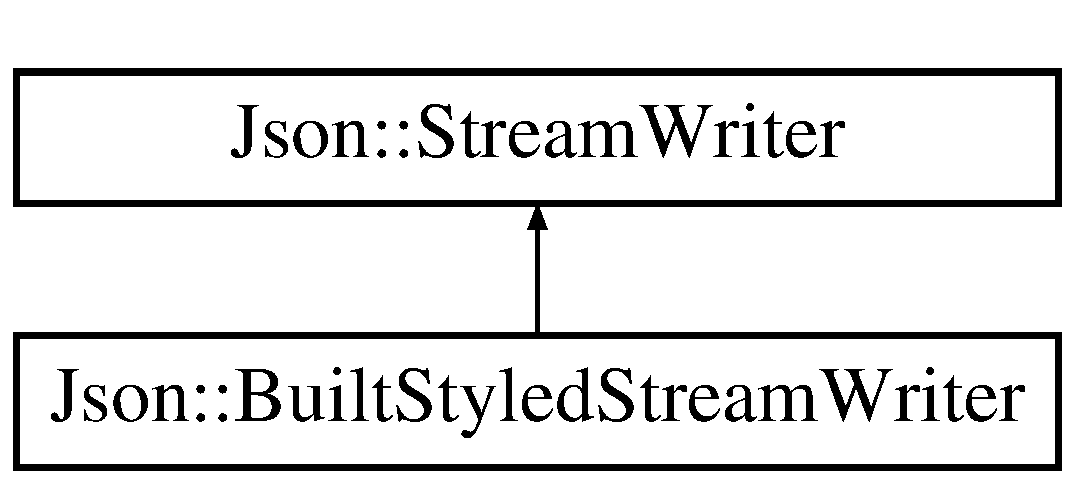
\includegraphics[height=2.000000cm]{structJson_1_1BuiltStyledStreamWriter}
\end{center}
\end{figure}
\subsection*{Public Member Functions}
\begin{DoxyCompactItemize}
\item 
\mbox{\Hypertarget{structJson_1_1BuiltStyledStreamWriter_adf11b7d1ee3c68d096b7c662ee85948e}\label{structJson_1_1BuiltStyledStreamWriter_adf11b7d1ee3c68d096b7c662ee85948e}} 
{\bfseries Built\+Styled\+Stream\+Writer} (J\+S\+O\+N\+C\+P\+P\+\_\+\+S\+T\+R\+I\+NG const \&indentation, \hyperlink{structJson_1_1CommentStyle_a51fc08f3518fd81eba12f340d19a3d0c}{Comment\+Style\+::\+Enum} cs, J\+S\+O\+N\+C\+P\+P\+\_\+\+S\+T\+R\+I\+NG const \&colon\+Symbol, J\+S\+O\+N\+C\+P\+P\+\_\+\+S\+T\+R\+I\+NG const \&null\+Symbol, J\+S\+O\+N\+C\+P\+P\+\_\+\+S\+T\+R\+I\+NG const \&ending\+Line\+Feed\+Symbol, bool use\+Special\+Floats, unsigned int precision)
\item 
int \hyperlink{structJson_1_1BuiltStyledStreamWriter_a823cdb1afabb6b0d5f39bcd5a6a6f747}{write} (\hyperlink{classJson_1_1Value}{Value} const \&root, J\+S\+O\+N\+C\+P\+P\+\_\+\+O\+S\+T\+R\+E\+AM $\ast$sout) J\+S\+O\+N\+C\+P\+P\+\_\+\+O\+V\+E\+R\+R\+I\+DE
\end{DoxyCompactItemize}
\subsection*{Additional Inherited Members}


\subsection{Member Function Documentation}
\mbox{\Hypertarget{structJson_1_1BuiltStyledStreamWriter_a823cdb1afabb6b0d5f39bcd5a6a6f747}\label{structJson_1_1BuiltStyledStreamWriter_a823cdb1afabb6b0d5f39bcd5a6a6f747}} 
\index{Json\+::\+Built\+Styled\+Stream\+Writer@{Json\+::\+Built\+Styled\+Stream\+Writer}!write@{write}}
\index{write@{write}!Json\+::\+Built\+Styled\+Stream\+Writer@{Json\+::\+Built\+Styled\+Stream\+Writer}}
\subsubsection{\texorpdfstring{write()}{write()}}
{\footnotesize\ttfamily int Json\+::\+Built\+Styled\+Stream\+Writer\+::write (\begin{DoxyParamCaption}\item[{\hyperlink{classJson_1_1Value}{Value} const \&}]{root,  }\item[{J\+S\+O\+N\+C\+P\+P\+\_\+\+O\+S\+T\+R\+E\+AM $\ast$}]{sout }\end{DoxyParamCaption})\hspace{0.3cm}{\ttfamily [virtual]}}

Write \hyperlink{classJson_1_1Value}{Value} into document as configured in sub-\/class. Do not take ownership of sout, but maintain a reference during function. \begin{DoxyPrecond}{Precondition}
sout != N\+U\+LL 
\end{DoxyPrecond}
\begin{DoxyReturn}{Returns}
zero on success (For now, we always return zero, so check the stream instead.) 
\end{DoxyReturn}

\begin{DoxyExceptions}{Exceptions}
{\em std\+::exception} & possibly, depending on configuration \\
\hline
\end{DoxyExceptions}


Implements \hyperlink{classJson_1_1StreamWriter_a84278bad0c9a9fc587bc2a97c5bb5993}{Json\+::\+Stream\+Writer}.



The documentation for this struct was generated from the following file\+:\begin{DoxyCompactItemize}
\item 
jsoncpp.\+cpp\end{DoxyCompactItemize}

\hypertarget{unionchar64long16}{}\section{char64long16 Union Reference}
\label{unionchar64long16}\index{char64long16@{char64long16}}
\subsection*{Public Attributes}
\begin{DoxyCompactItemize}
\item 
\mbox{\Hypertarget{unionchar64long16_a7067dbe3b0ff3f11661acb8cd97bcff9}\label{unionchar64long16_a7067dbe3b0ff3f11661acb8cd97bcff9}} 
unsigned char {\bfseries c} \mbox{[}64\mbox{]}
\item 
\mbox{\Hypertarget{unionchar64long16_a4f1edebae3468a551ff2d0cdaecb467d}\label{unionchar64long16_a4f1edebae3468a551ff2d0cdaecb467d}} 
uint32\+\_\+t {\bfseries l} \mbox{[}16\mbox{]}
\end{DoxyCompactItemize}


The documentation for this union was generated from the following file\+:\begin{DoxyCompactItemize}
\item 
mongoose.\+c\end{DoxyCompactItemize}

\hypertarget{classJson_1_1CharReader}{}\section{Json\+:\+:Char\+Reader Class Reference}
\label{classJson_1_1CharReader}\index{Json\+::\+Char\+Reader@{Json\+::\+Char\+Reader}}


{\ttfamily \#include $<$json.\+h$>$}

Inheritance diagram for Json\+:\+:Char\+Reader\+:\begin{figure}[H]
\begin{center}
\leavevmode
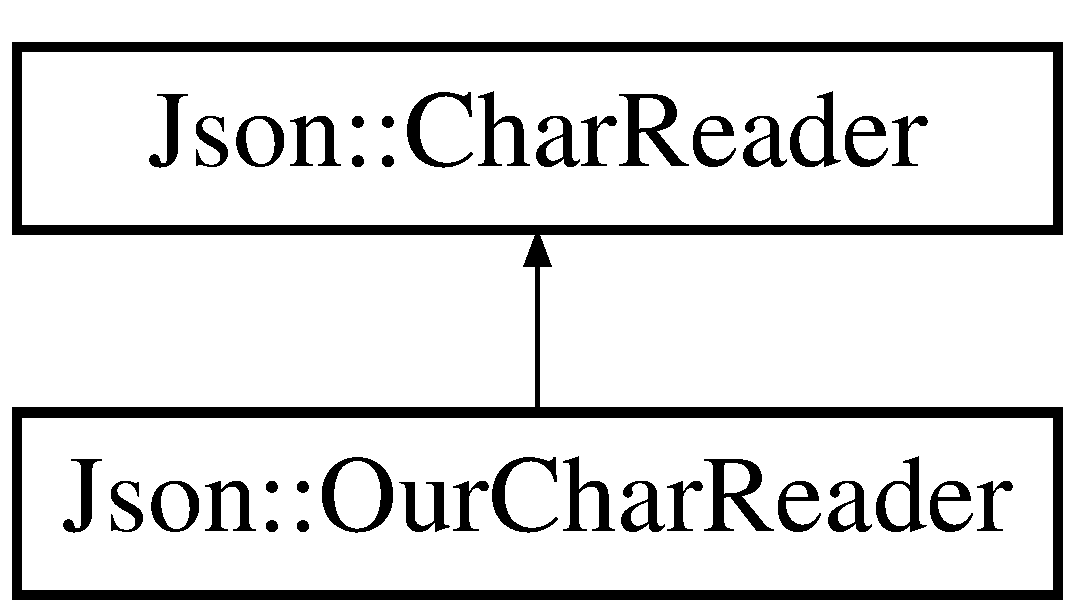
\includegraphics[height=2.000000cm]{classJson_1_1CharReader}
\end{center}
\end{figure}
\subsection*{Classes}
\begin{DoxyCompactItemize}
\item 
class \hyperlink{classJson_1_1CharReader_1_1Factory}{Factory}
\end{DoxyCompactItemize}
\subsection*{Public Member Functions}
\begin{DoxyCompactItemize}
\item 
virtual \hyperlink{classJson_1_1CharReader_acaa7b6ad04fe1cf2ddfca06e66550d7e_acaa7b6ad04fe1cf2ddfca06e66550d7e}{$\sim$\+Char\+Reader} ()
\item 
virtual bool \hyperlink{classJson_1_1CharReader_a7983680d50fd0745f371c43b162e78e1_a7983680d50fd0745f371c43b162e78e1}{parse} (char const $\ast$begin\+Doc, char const $\ast$end\+Doc, \hyperlink{classJson_1_1Value}{Value} $\ast$root, \hyperlink{json_8h_a1e723f95759de062585bc4a8fd3fa4be_a1e723f95759de062585bc4a8fd3fa4be}{J\+S\+O\+N\+C\+P\+P\+\_\+\+S\+T\+R\+I\+NG} $\ast$errs)=0
\begin{DoxyCompactList}\small\item\em Read a \hyperlink{classJson_1_1Value}{Value} from a \href{http://www.json.org}{\tt J\+S\+ON} document. The document must be a U\+T\+F-\/8 encoded string containing the document to read. \end{DoxyCompactList}\end{DoxyCompactItemize}


\subsection{Detailed Description}
Interface for reading J\+S\+ON from a char array. 

\subsection{Constructor \& Destructor Documentation}
\mbox{\Hypertarget{classJson_1_1CharReader_acaa7b6ad04fe1cf2ddfca06e66550d7e_acaa7b6ad04fe1cf2ddfca06e66550d7e}\label{classJson_1_1CharReader_acaa7b6ad04fe1cf2ddfca06e66550d7e_acaa7b6ad04fe1cf2ddfca06e66550d7e}} 
\index{Json\+::\+Char\+Reader@{Json\+::\+Char\+Reader}!````~Char\+Reader@{$\sim$\+Char\+Reader}}
\index{````~Char\+Reader@{$\sim$\+Char\+Reader}!Json\+::\+Char\+Reader@{Json\+::\+Char\+Reader}}
\subsubsection{\texorpdfstring{$\sim$\+Char\+Reader()}{~CharReader()}}
{\footnotesize\ttfamily virtual Json\+::\+Char\+Reader\+::$\sim$\+Char\+Reader (\begin{DoxyParamCaption}{ }\end{DoxyParamCaption})\hspace{0.3cm}{\ttfamily [inline]}, {\ttfamily [virtual]}}



References J\+S\+O\+N\+C\+P\+P\+\_\+\+S\+T\+R\+I\+NG.



\subsection{Member Function Documentation}
\mbox{\Hypertarget{classJson_1_1CharReader_a7983680d50fd0745f371c43b162e78e1_a7983680d50fd0745f371c43b162e78e1}\label{classJson_1_1CharReader_a7983680d50fd0745f371c43b162e78e1_a7983680d50fd0745f371c43b162e78e1}} 
\index{Json\+::\+Char\+Reader@{Json\+::\+Char\+Reader}!parse@{parse}}
\index{parse@{parse}!Json\+::\+Char\+Reader@{Json\+::\+Char\+Reader}}
\subsubsection{\texorpdfstring{parse()}{parse()}}
{\footnotesize\ttfamily virtual bool Json\+::\+Char\+Reader\+::parse (\begin{DoxyParamCaption}\item[{char const $\ast$}]{begin\+Doc,  }\item[{char const $\ast$}]{end\+Doc,  }\item[{\hyperlink{classJson_1_1Value}{Value} $\ast$}]{root,  }\item[{\hyperlink{json_8h_a1e723f95759de062585bc4a8fd3fa4be_a1e723f95759de062585bc4a8fd3fa4be}{J\+S\+O\+N\+C\+P\+P\+\_\+\+S\+T\+R\+I\+NG} $\ast$}]{errs }\end{DoxyParamCaption})\hspace{0.3cm}{\ttfamily [pure virtual]}}



Read a \hyperlink{classJson_1_1Value}{Value} from a \href{http://www.json.org}{\tt J\+S\+ON} document. The document must be a U\+T\+F-\/8 encoded string containing the document to read. 


\begin{DoxyParams}{Parameters}
{\em begin\+Doc} & Pointer on the beginning of the U\+T\+F-\/8 encoded string of the document to read. \\
\hline
{\em end\+Doc} & Pointer on the end of the U\+T\+F-\/8 encoded string of the document to read. Must be $>$= begin\+Doc. \\
\hline
{\em root} & \mbox{[}out\mbox{]} Contains the root value of the document if it was successfully parsed. \\
\hline
{\em errs} & \mbox{[}out\mbox{]} Formatted error messages (if not N\+U\+LL) a user friendly string that lists errors in the parsed document. \\
\hline
\end{DoxyParams}
\begin{DoxyReturn}{Returns}
{\ttfamily true} if the document was successfully parsed, {\ttfamily false} if an error occurred. 
\end{DoxyReturn}


Implemented in \hyperlink{classJson_1_1OurCharReader_a547f08ec5a9951ca69e8bb2e90296c83_a547f08ec5a9951ca69e8bb2e90296c83}{Json\+::\+Our\+Char\+Reader}.



The documentation for this class was generated from the following file\+:\begin{DoxyCompactItemize}
\item 
json/\hyperlink{json_8h}{json.\+h}\end{DoxyCompactItemize}

\hypertarget{classJson_1_1CharReaderBuilder}{}\section{Json\+:\+:Char\+Reader\+Builder Class Reference}
\label{classJson_1_1CharReaderBuilder}\index{Json\+::\+Char\+Reader\+Builder@{Json\+::\+Char\+Reader\+Builder}}


Build a \hyperlink{classJson_1_1CharReader}{Char\+Reader} implementation.  




{\ttfamily \#include $<$json.\+h$>$}

Inheritance diagram for Json\+:\+:Char\+Reader\+Builder\+:\begin{figure}[H]
\begin{center}
\leavevmode
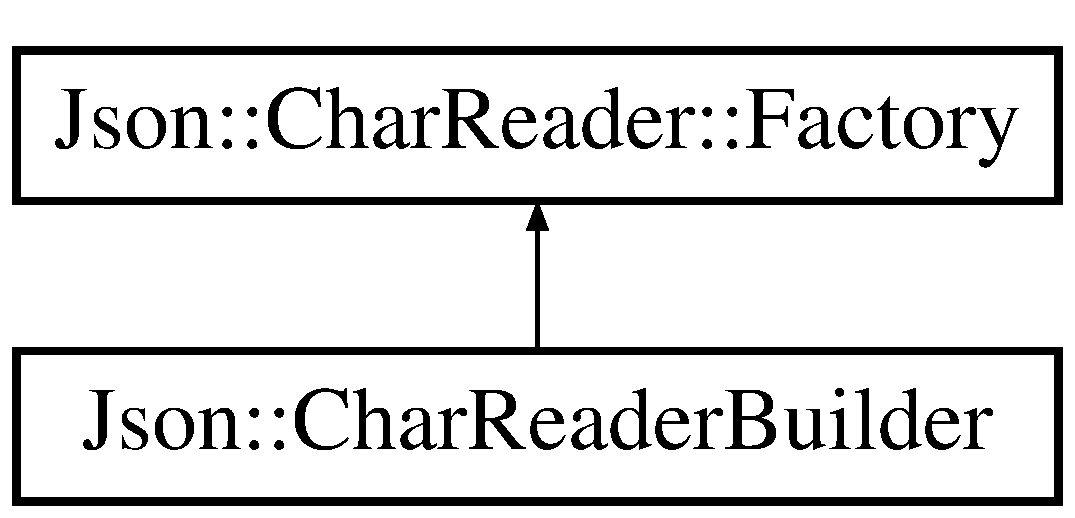
\includegraphics[height=2.000000cm]{classJson_1_1CharReaderBuilder}
\end{center}
\end{figure}
\subsection*{Public Member Functions}
\begin{DoxyCompactItemize}
\item 
\hyperlink{classJson_1_1CharReader}{Char\+Reader} $\ast$ \hyperlink{classJson_1_1CharReaderBuilder_a3a262fcc76c1eb8eebfd4718fb4e9722}{new\+Char\+Reader} () const J\+S\+O\+N\+C\+P\+P\+\_\+\+O\+V\+E\+R\+R\+I\+DE
\begin{DoxyCompactList}\small\item\em Allocate a \hyperlink{classJson_1_1CharReader}{Char\+Reader} via operator new(). \end{DoxyCompactList}\item 
bool \hyperlink{classJson_1_1CharReaderBuilder_af890b5cb70e9b372e41de5c9e6535d21}{validate} (\hyperlink{classJson_1_1Value}{Json\+::\+Value} $\ast$invalid) const
\item 
\hyperlink{classJson_1_1Value}{Value} \& \hyperlink{classJson_1_1CharReaderBuilder_a84b35ef443340c06c0aa7b47851d8d86}{operator\mbox{[}$\,$\mbox{]}} (J\+S\+O\+N\+C\+P\+P\+\_\+\+S\+T\+R\+I\+NG key)
\end{DoxyCompactItemize}
\subsection*{Static Public Member Functions}
\begin{DoxyCompactItemize}
\item 
static void \hyperlink{classJson_1_1CharReaderBuilder_a03ff031e06aabff989ab4addc87294ab}{set\+Defaults} (\hyperlink{classJson_1_1Value}{Json\+::\+Value} $\ast$settings)
\item 
static void \hyperlink{classJson_1_1CharReaderBuilder_a9c19e3c5475f9072d527810d4bf56749}{strict\+Mode} (\hyperlink{classJson_1_1Value}{Json\+::\+Value} $\ast$settings)
\end{DoxyCompactItemize}
\subsection*{Public Attributes}
\begin{DoxyCompactItemize}
\item 
\hyperlink{classJson_1_1Value}{Json\+::\+Value} \hyperlink{classJson_1_1CharReaderBuilder_ac69b7911ad64c171c51ebaf2ea26d958}{settings\+\_\+}
\end{DoxyCompactItemize}


\subsection{Detailed Description}
Build a \hyperlink{classJson_1_1CharReader}{Char\+Reader} implementation. 

Usage\+: 
\begin{DoxyCode}
\textcolor{keyword}{using namespace }\hyperlink{namespaceJson}{Json};
\hyperlink{classJson_1_1CharReaderBuilder}{CharReaderBuilder} builder;
builder[\textcolor{stringliteral}{"collectComments"}] = \textcolor{keyword}{false};
\hyperlink{classJson_1_1Value}{Value} value;
JSONCPP\_STRING errs;
\textcolor{keywordtype}{bool} ok = \hyperlink{namespaceJson_aab0cf1ecf81d1aeca12be2a416a84352}{parseFromStream}(builder, std::cin, &value, &errs);
\end{DoxyCode}
 

\subsection{Member Function Documentation}
\mbox{\Hypertarget{classJson_1_1CharReaderBuilder_a3a262fcc76c1eb8eebfd4718fb4e9722}\label{classJson_1_1CharReaderBuilder_a3a262fcc76c1eb8eebfd4718fb4e9722}} 
\index{Json\+::\+Char\+Reader\+Builder@{Json\+::\+Char\+Reader\+Builder}!new\+Char\+Reader@{new\+Char\+Reader}}
\index{new\+Char\+Reader@{new\+Char\+Reader}!Json\+::\+Char\+Reader\+Builder@{Json\+::\+Char\+Reader\+Builder}}
\subsubsection{\texorpdfstring{new\+Char\+Reader()}{newCharReader()}}
{\footnotesize\ttfamily \hyperlink{classJson_1_1CharReader}{Char\+Reader} $\ast$ Json\+::\+Char\+Reader\+Builder\+::new\+Char\+Reader (\begin{DoxyParamCaption}{ }\end{DoxyParamCaption}) const\hspace{0.3cm}{\ttfamily [virtual]}}



Allocate a \hyperlink{classJson_1_1CharReader}{Char\+Reader} via operator new(). 


\begin{DoxyExceptions}{Exceptions}
{\em std\+::exception} & if something goes wrong (e.\+g. invalid settings) \\
\hline
\end{DoxyExceptions}


Implements \hyperlink{classJson_1_1CharReader_1_1Factory_a4c5862a1ffd432372dbe65cf59de98c4}{Json\+::\+Char\+Reader\+::\+Factory}.

\mbox{\Hypertarget{classJson_1_1CharReaderBuilder_a84b35ef443340c06c0aa7b47851d8d86}\label{classJson_1_1CharReaderBuilder_a84b35ef443340c06c0aa7b47851d8d86}} 
\index{Json\+::\+Char\+Reader\+Builder@{Json\+::\+Char\+Reader\+Builder}!operator\mbox{[}\mbox{]}@{operator[]}}
\index{operator\mbox{[}\mbox{]}@{operator[]}!Json\+::\+Char\+Reader\+Builder@{Json\+::\+Char\+Reader\+Builder}}
\subsubsection{\texorpdfstring{operator[]()}{operator[]()}}
{\footnotesize\ttfamily \hyperlink{classJson_1_1Value}{Value} \& Json\+::\+Char\+Reader\+Builder\+::operator\mbox{[}$\,$\mbox{]} (\begin{DoxyParamCaption}\item[{J\+S\+O\+N\+C\+P\+P\+\_\+\+S\+T\+R\+I\+NG}]{key }\end{DoxyParamCaption})}

A simple way to update a specific setting. \mbox{\Hypertarget{classJson_1_1CharReaderBuilder_a03ff031e06aabff989ab4addc87294ab}\label{classJson_1_1CharReaderBuilder_a03ff031e06aabff989ab4addc87294ab}} 
\index{Json\+::\+Char\+Reader\+Builder@{Json\+::\+Char\+Reader\+Builder}!set\+Defaults@{set\+Defaults}}
\index{set\+Defaults@{set\+Defaults}!Json\+::\+Char\+Reader\+Builder@{Json\+::\+Char\+Reader\+Builder}}
\subsubsection{\texorpdfstring{set\+Defaults()}{setDefaults()}}
{\footnotesize\ttfamily void Json\+::\+Char\+Reader\+Builder\+::set\+Defaults (\begin{DoxyParamCaption}\item[{\hyperlink{classJson_1_1Value}{Json\+::\+Value} $\ast$}]{settings }\end{DoxyParamCaption})\hspace{0.3cm}{\ttfamily [static]}}

Called by ctor, but you can use this to reset settings\+\_\+. \begin{DoxyPrecond}{Precondition}
\textquotesingle{}settings\textquotesingle{} != N\+U\+LL (but Json\+::null is fine) 
\end{DoxyPrecond}
\begin{DoxyRemark}{Remarks}
Defaults\+: 
\begin{DoxyCodeInclude}
\end{DoxyCodeInclude}

\end{DoxyRemark}
\mbox{[}Char\+Reader\+Builder\+Defaults\mbox{]}

\mbox{[}Char\+Reader\+Builder\+Defaults\mbox{]} \mbox{\Hypertarget{classJson_1_1CharReaderBuilder_a9c19e3c5475f9072d527810d4bf56749}\label{classJson_1_1CharReaderBuilder_a9c19e3c5475f9072d527810d4bf56749}} 
\index{Json\+::\+Char\+Reader\+Builder@{Json\+::\+Char\+Reader\+Builder}!strict\+Mode@{strict\+Mode}}
\index{strict\+Mode@{strict\+Mode}!Json\+::\+Char\+Reader\+Builder@{Json\+::\+Char\+Reader\+Builder}}
\subsubsection{\texorpdfstring{strict\+Mode()}{strictMode()}}
{\footnotesize\ttfamily void Json\+::\+Char\+Reader\+Builder\+::strict\+Mode (\begin{DoxyParamCaption}\item[{\hyperlink{classJson_1_1Value}{Json\+::\+Value} $\ast$}]{settings }\end{DoxyParamCaption})\hspace{0.3cm}{\ttfamily [static]}}

Same as old \hyperlink{classJson_1_1Features_ae23176c14b2e79e81fb61fb1a8ab58ee}{Features\+::strict\+Mode()}. \begin{DoxyPrecond}{Precondition}
\textquotesingle{}settings\textquotesingle{} != N\+U\+LL (but Json\+::null is fine) 
\end{DoxyPrecond}
\begin{DoxyRemark}{Remarks}
Defaults\+: 
\begin{DoxyCodeInclude}
\end{DoxyCodeInclude}

\end{DoxyRemark}
\mbox{[}Char\+Reader\+Builder\+Strict\+Mode\mbox{]}

\mbox{[}Char\+Reader\+Builder\+Strict\+Mode\mbox{]} \mbox{\Hypertarget{classJson_1_1CharReaderBuilder_af890b5cb70e9b372e41de5c9e6535d21}\label{classJson_1_1CharReaderBuilder_af890b5cb70e9b372e41de5c9e6535d21}} 
\index{Json\+::\+Char\+Reader\+Builder@{Json\+::\+Char\+Reader\+Builder}!validate@{validate}}
\index{validate@{validate}!Json\+::\+Char\+Reader\+Builder@{Json\+::\+Char\+Reader\+Builder}}
\subsubsection{\texorpdfstring{validate()}{validate()}}
{\footnotesize\ttfamily bool Json\+::\+Char\+Reader\+Builder\+::validate (\begin{DoxyParamCaption}\item[{\hyperlink{classJson_1_1Value}{Json\+::\+Value} $\ast$}]{invalid }\end{DoxyParamCaption}) const}

\begin{DoxyReturn}{Returns}
true if \textquotesingle{}settings\textquotesingle{} are legal and consistent; otherwise, indicate bad settings via \textquotesingle{}invalid\textquotesingle{}. 
\end{DoxyReturn}


\subsection{Member Data Documentation}
\mbox{\Hypertarget{classJson_1_1CharReaderBuilder_ac69b7911ad64c171c51ebaf2ea26d958}\label{classJson_1_1CharReaderBuilder_ac69b7911ad64c171c51ebaf2ea26d958}} 
\index{Json\+::\+Char\+Reader\+Builder@{Json\+::\+Char\+Reader\+Builder}!settings\+\_\+@{settings\+\_\+}}
\index{settings\+\_\+@{settings\+\_\+}!Json\+::\+Char\+Reader\+Builder@{Json\+::\+Char\+Reader\+Builder}}
\subsubsection{\texorpdfstring{settings\+\_\+}{settings\_}}
{\footnotesize\ttfamily \hyperlink{classJson_1_1Value}{Json\+::\+Value} Json\+::\+Char\+Reader\+Builder\+::settings\+\_\+}

Configuration of this builder. These are case-\/sensitive. Available settings (case-\/sensitive)\+:
\begin{DoxyItemize}
\item {\ttfamily \char`\"{}collect\+Comments\char`\"{}\+: false or true}
\begin{DoxyItemize}
\item true to collect comment and allow writing them back during serialization, false to discard comments. This parameter is ignored if allow\+Comments is false.
\end{DoxyItemize}
\item {\ttfamily \char`\"{}allow\+Comments\char`\"{}\+: false or true}
\begin{DoxyItemize}
\item true if comments are allowed.
\end{DoxyItemize}
\item {\ttfamily \char`\"{}strict\+Root\char`\"{}\+: false or true}
\begin{DoxyItemize}
\item true if root must be either an array or an object value
\end{DoxyItemize}
\item {\ttfamily \char`\"{}allow\+Dropped\+Null\+Placeholders\char`\"{}\+: false or true}
\begin{DoxyItemize}
\item true if dropped null placeholders are allowed. (See \hyperlink{classJson_1_1StreamWriterBuilder}{Stream\+Writer\+Builder}.)
\end{DoxyItemize}
\item {\ttfamily \char`\"{}allow\+Numeric\+Keys\char`\"{}\+: false or true}
\begin{DoxyItemize}
\item true if numeric object keys are allowed.
\end{DoxyItemize}
\item {\ttfamily \char`\"{}allow\+Single\+Quotes\char`\"{}\+: false or true}
\begin{DoxyItemize}
\item true if \textquotesingle{}\textquotesingle{} are allowed for strings (both keys and values)
\end{DoxyItemize}
\item {\ttfamily \char`\"{}stack\+Limit\char`\"{}\+: integer}
\begin{DoxyItemize}
\item Exceeding stack\+Limit (recursive depth of {\ttfamily read\+Value()}) will cause an exception.
\item This is a security issue (seg-\/faults caused by deeply nested J\+S\+ON), so the default is low.
\end{DoxyItemize}
\item {\ttfamily \char`\"{}fail\+If\+Extra\char`\"{}\+: false or true}
\begin{DoxyItemize}
\item If true, {\ttfamily parse()} returns false when extra non-\/whitespace trails the J\+S\+ON value in the input string.
\end{DoxyItemize}
\item {\ttfamily \char`\"{}reject\+Dup\+Keys\char`\"{}\+: false or true}
\begin{DoxyItemize}
\item If true, {\ttfamily parse()} returns false when a key is duplicated within an object.
\end{DoxyItemize}
\item {\ttfamily \char`\"{}allow\+Special\+Floats\char`\"{}\+: false or true}
\begin{DoxyItemize}
\item If true, special float values (Na\+Ns and infinities) are allowed and their values are lossfree restorable.
\end{DoxyItemize}
\end{DoxyItemize}

You can examine \textquotesingle{}settings\+\_\+` yourself to see the defaults. You can also write and read them just like any J\+S\+ON \hyperlink{classJson_1_1Value}{Value}. \begin{DoxySeeAlso}{See also}
\hyperlink{classJson_1_1CharReaderBuilder_a03ff031e06aabff989ab4addc87294ab}{set\+Defaults()} 
\end{DoxySeeAlso}


The documentation for this class was generated from the following files\+:\begin{DoxyCompactItemize}
\item 
json/json.\+h\item 
jsoncpp.\+cpp\end{DoxyCompactItemize}

\hypertarget{classTBT_1_1Client}{}\section{T\+BT\+:\+:Client Class Reference}
\label{classTBT_1_1Client}\index{T\+B\+T\+::\+Client@{T\+B\+T\+::\+Client}}
Inheritance diagram for T\+BT\+:\+:Client\+:\begin{figure}[H]
\begin{center}
\leavevmode
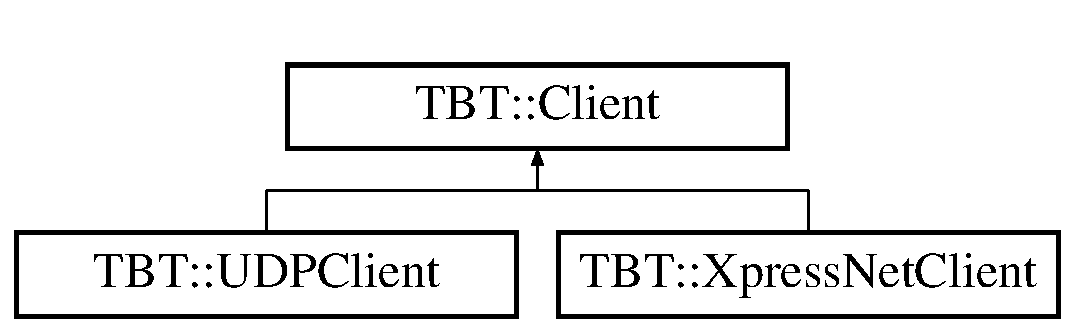
\includegraphics[height=2.000000cm]{classTBT_1_1Client}
\end{center}
\end{figure}
\subsection*{Public Member Functions}
\begin{DoxyCompactItemize}
\item 
\mbox{\Hypertarget{classTBT_1_1Client_a6220a6ee1345c62986aea535e2ae202c}\label{classTBT_1_1Client_a6220a6ee1345c62986aea535e2ae202c}} 
{\bfseries Client} (\hyperlink{classTBT_1_1ClientInterface}{Client\+Interface} $\ast$p\+Interface)
\item 
\mbox{\Hypertarget{classTBT_1_1Client_a37d9a9919aa90879dbf46cf95e519259}\label{classTBT_1_1Client_a37d9a9919aa90879dbf46cf95e519259}} 
\hyperlink{classTBT_1_1ClientInterface}{Client\+Interface} $\ast$ {\bfseries get\+Interface} (void)
\item 
\mbox{\Hypertarget{classTBT_1_1Client_ad64588b494ec98154ea261ed4f3b3643}\label{classTBT_1_1Client_ad64588b494ec98154ea261ed4f3b3643}} 
virtual void {\bfseries broadcast\+Power\+State\+Change} (bool new\+State)=0
\item 
\mbox{\Hypertarget{classTBT_1_1Client_aeb3b63a37edc6b95872df54a57c27a71}\label{classTBT_1_1Client_aeb3b63a37edc6b95872df54a57c27a71}} 
virtual void {\bfseries broadcast\+Loc\+Info\+Changed} (\hyperlink{classTBT_1_1LocDecoder}{Loc\+Decoder} $\ast$p\+Loc)=0
\item 
\mbox{\Hypertarget{classTBT_1_1Client_a59459df809a663bcbbb6d31fbfa09402}\label{classTBT_1_1Client_a59459df809a663bcbbb6d31fbfa09402}} 
virtual void {\bfseries broadcast\+Emergency\+Stop} (void)=0
\end{DoxyCompactItemize}
\subsection*{Protected Attributes}
\begin{DoxyCompactItemize}
\item 
\mbox{\Hypertarget{classTBT_1_1Client_a0b3e41f73f6381600c8ddac129b740f6}\label{classTBT_1_1Client_a0b3e41f73f6381600c8ddac129b740f6}} 
\hyperlink{classTBT_1_1ClientInterface}{Client\+Interface} $\ast$ {\bfseries m\+\_\+p\+Interface}
\end{DoxyCompactItemize}


The documentation for this class was generated from the following files\+:\begin{DoxyCompactItemize}
\item 
Client.\+h\item 
Client.\+cpp\end{DoxyCompactItemize}

\hypertarget{classTBT_1_1ClientInterface}{}\section{T\+BT\+:\+:Client\+Interface Class Reference}
\label{classTBT_1_1ClientInterface}\index{T\+B\+T\+::\+Client\+Interface@{T\+B\+T\+::\+Client\+Interface}}


{\ttfamily \#include $<$Client\+Interface.\+h$>$}

Inheritance diagram for T\+BT\+:\+:Client\+Interface\+:\begin{figure}[H]
\begin{center}
\leavevmode
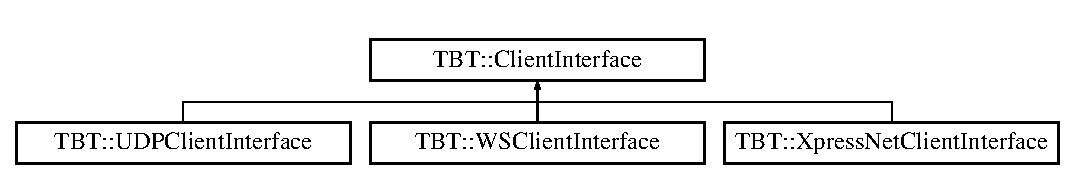
\includegraphics[height=1.975309cm]{classTBT_1_1ClientInterface}
\end{center}
\end{figure}
\subsection*{Public Member Functions}
\begin{DoxyCompactItemize}
\item 
\hyperlink{classTBT_1_1ClientInterface_a77cd35b080e78932f2371ea0f897964b_a77cd35b080e78932f2371ea0f897964b}{Client\+Interface} (\hyperlink{classTBT_1_1Manager}{Manager} $\ast$p\+Manager)
\item 
virtual \hyperlink{classTBT_1_1ClientInterface_aa42abb5947fa0af75eed777325cbff27_aa42abb5947fa0af75eed777325cbff27}{$\sim$\+Client\+Interface} ()
\item 
\hyperlink{classTBT_1_1Manager}{Manager} $\ast$ \hyperlink{classTBT_1_1ClientInterface_a26e144856b1253744b20c5638065acf7_a26e144856b1253744b20c5638065acf7}{get\+Manager} (void)
\item 
virtual void \hyperlink{classTBT_1_1ClientInterface_a7888a3446fb416fad75e5e008a85ca0c_a7888a3446fb416fad75e5e008a85ca0c}{broadcast\+Power\+State\+Change} (bool new\+State)=0
\item 
virtual void \hyperlink{classTBT_1_1ClientInterface_aaede3709fa0dcb23743f43d9c1a5ab04_aaede3709fa0dcb23743f43d9c1a5ab04}{broadcast\+Loc\+Info\+Change} (\hyperlink{classTBT_1_1LocDecoder}{Loc\+Decoder} $\ast$p\+Loc)=0
\item 
virtual void \hyperlink{classTBT_1_1ClientInterface_a8d19220baccb47a7c9f45d0288bebcb8_a8d19220baccb47a7c9f45d0288bebcb8}{broadcast\+Emergency\+Stop} (void)=0
\end{DoxyCompactItemize}
\subsection*{Protected Attributes}
\begin{DoxyCompactItemize}
\item 
\hyperlink{classTBT_1_1Manager}{Manager} $\ast$ \hyperlink{classTBT_1_1ClientInterface_a1d6558ab5cd2ebcc135e5fc37a1844ba_a1d6558ab5cd2ebcc135e5fc37a1844ba}{m\+\_\+p\+Manager}
\end{DoxyCompactItemize}


\subsection{Constructor \& Destructor Documentation}
\mbox{\Hypertarget{classTBT_1_1ClientInterface_a77cd35b080e78932f2371ea0f897964b_a77cd35b080e78932f2371ea0f897964b}\label{classTBT_1_1ClientInterface_a77cd35b080e78932f2371ea0f897964b_a77cd35b080e78932f2371ea0f897964b}} 
\index{T\+B\+T\+::\+Client\+Interface@{T\+B\+T\+::\+Client\+Interface}!Client\+Interface@{Client\+Interface}}
\index{Client\+Interface@{Client\+Interface}!T\+B\+T\+::\+Client\+Interface@{T\+B\+T\+::\+Client\+Interface}}
\subsubsection{\texorpdfstring{Client\+Interface()}{ClientInterface()}}
{\footnotesize\ttfamily T\+B\+T\+::\+Client\+Interface\+::\+Client\+Interface (\begin{DoxyParamCaption}\item[{\hyperlink{classTBT_1_1Manager}{Manager} $\ast$}]{p\+Manager }\end{DoxyParamCaption})}

\mbox{\Hypertarget{classTBT_1_1ClientInterface_aa42abb5947fa0af75eed777325cbff27_aa42abb5947fa0af75eed777325cbff27}\label{classTBT_1_1ClientInterface_aa42abb5947fa0af75eed777325cbff27_aa42abb5947fa0af75eed777325cbff27}} 
\index{T\+B\+T\+::\+Client\+Interface@{T\+B\+T\+::\+Client\+Interface}!````~Client\+Interface@{$\sim$\+Client\+Interface}}
\index{````~Client\+Interface@{$\sim$\+Client\+Interface}!T\+B\+T\+::\+Client\+Interface@{T\+B\+T\+::\+Client\+Interface}}
\subsubsection{\texorpdfstring{$\sim$\+Client\+Interface()}{~ClientInterface()}}
{\footnotesize\ttfamily T\+B\+T\+::\+Client\+Interface\+::$\sim$\+Client\+Interface (\begin{DoxyParamCaption}{ }\end{DoxyParamCaption})\hspace{0.3cm}{\ttfamily [virtual]}}



\subsection{Member Function Documentation}
\mbox{\Hypertarget{classTBT_1_1ClientInterface_a8d19220baccb47a7c9f45d0288bebcb8_a8d19220baccb47a7c9f45d0288bebcb8}\label{classTBT_1_1ClientInterface_a8d19220baccb47a7c9f45d0288bebcb8_a8d19220baccb47a7c9f45d0288bebcb8}} 
\index{T\+B\+T\+::\+Client\+Interface@{T\+B\+T\+::\+Client\+Interface}!broadcast\+Emergency\+Stop@{broadcast\+Emergency\+Stop}}
\index{broadcast\+Emergency\+Stop@{broadcast\+Emergency\+Stop}!T\+B\+T\+::\+Client\+Interface@{T\+B\+T\+::\+Client\+Interface}}
\subsubsection{\texorpdfstring{broadcast\+Emergency\+Stop()}{broadcastEmergencyStop()}}
{\footnotesize\ttfamily virtual void T\+B\+T\+::\+Client\+Interface\+::broadcast\+Emergency\+Stop (\begin{DoxyParamCaption}\item[{void}]{ }\end{DoxyParamCaption})\hspace{0.3cm}{\ttfamily [pure virtual]}}



Implemented in \hyperlink{classTBT_1_1UDPClientInterface_a33a0c51d141a457cda9dacc4d82d5304_a33a0c51d141a457cda9dacc4d82d5304}{T\+B\+T\+::\+U\+D\+P\+Client\+Interface}, \hyperlink{classTBT_1_1WSClientInterface_a2ad439e557711c57c8a978e3b6efcb62_a2ad439e557711c57c8a978e3b6efcb62}{T\+B\+T\+::\+W\+S\+Client\+Interface}, and \hyperlink{classTBT_1_1XpressNetClientInterface_a143641241f4830f22ec5beb78036ce4c_a143641241f4830f22ec5beb78036ce4c}{T\+B\+T\+::\+Xpress\+Net\+Client\+Interface}.



Referenced by get\+Manager().

\mbox{\Hypertarget{classTBT_1_1ClientInterface_aaede3709fa0dcb23743f43d9c1a5ab04_aaede3709fa0dcb23743f43d9c1a5ab04}\label{classTBT_1_1ClientInterface_aaede3709fa0dcb23743f43d9c1a5ab04_aaede3709fa0dcb23743f43d9c1a5ab04}} 
\index{T\+B\+T\+::\+Client\+Interface@{T\+B\+T\+::\+Client\+Interface}!broadcast\+Loc\+Info\+Change@{broadcast\+Loc\+Info\+Change}}
\index{broadcast\+Loc\+Info\+Change@{broadcast\+Loc\+Info\+Change}!T\+B\+T\+::\+Client\+Interface@{T\+B\+T\+::\+Client\+Interface}}
\subsubsection{\texorpdfstring{broadcast\+Loc\+Info\+Change()}{broadcastLocInfoChange()}}
{\footnotesize\ttfamily virtual void T\+B\+T\+::\+Client\+Interface\+::broadcast\+Loc\+Info\+Change (\begin{DoxyParamCaption}\item[{\hyperlink{classTBT_1_1LocDecoder}{Loc\+Decoder} $\ast$}]{p\+Loc }\end{DoxyParamCaption})\hspace{0.3cm}{\ttfamily [pure virtual]}}



Implemented in \hyperlink{classTBT_1_1UDPClientInterface_af4e63115b3156b151d4dfd50342b36e7_af4e63115b3156b151d4dfd50342b36e7}{T\+B\+T\+::\+U\+D\+P\+Client\+Interface}, \hyperlink{classTBT_1_1WSClientInterface_a39806206461815c06c517b66d122b4db_a39806206461815c06c517b66d122b4db}{T\+B\+T\+::\+W\+S\+Client\+Interface}, and \hyperlink{classTBT_1_1XpressNetClientInterface_a8e64404cb84913c2d9290d2afb882b39_a8e64404cb84913c2d9290d2afb882b39}{T\+B\+T\+::\+Xpress\+Net\+Client\+Interface}.



Referenced by get\+Manager().

\mbox{\Hypertarget{classTBT_1_1ClientInterface_a7888a3446fb416fad75e5e008a85ca0c_a7888a3446fb416fad75e5e008a85ca0c}\label{classTBT_1_1ClientInterface_a7888a3446fb416fad75e5e008a85ca0c_a7888a3446fb416fad75e5e008a85ca0c}} 
\index{T\+B\+T\+::\+Client\+Interface@{T\+B\+T\+::\+Client\+Interface}!broadcast\+Power\+State\+Change@{broadcast\+Power\+State\+Change}}
\index{broadcast\+Power\+State\+Change@{broadcast\+Power\+State\+Change}!T\+B\+T\+::\+Client\+Interface@{T\+B\+T\+::\+Client\+Interface}}
\subsubsection{\texorpdfstring{broadcast\+Power\+State\+Change()}{broadcastPowerStateChange()}}
{\footnotesize\ttfamily virtual void T\+B\+T\+::\+Client\+Interface\+::broadcast\+Power\+State\+Change (\begin{DoxyParamCaption}\item[{bool}]{new\+State }\end{DoxyParamCaption})\hspace{0.3cm}{\ttfamily [pure virtual]}}



Implemented in \hyperlink{classTBT_1_1UDPClientInterface_a60ddc3657a12b4e6c7ef7db0a31c9e3c_a60ddc3657a12b4e6c7ef7db0a31c9e3c}{T\+B\+T\+::\+U\+D\+P\+Client\+Interface}, \hyperlink{classTBT_1_1WSClientInterface_ad1c7f413c63f04b04d6e20f5d154d1fd_ad1c7f413c63f04b04d6e20f5d154d1fd}{T\+B\+T\+::\+W\+S\+Client\+Interface}, and \hyperlink{classTBT_1_1XpressNetClientInterface_a338da1925ec68f197e87625c7497f472_a338da1925ec68f197e87625c7497f472}{T\+B\+T\+::\+Xpress\+Net\+Client\+Interface}.



Referenced by get\+Manager().

\mbox{\Hypertarget{classTBT_1_1ClientInterface_a26e144856b1253744b20c5638065acf7_a26e144856b1253744b20c5638065acf7}\label{classTBT_1_1ClientInterface_a26e144856b1253744b20c5638065acf7_a26e144856b1253744b20c5638065acf7}} 
\index{T\+B\+T\+::\+Client\+Interface@{T\+B\+T\+::\+Client\+Interface}!get\+Manager@{get\+Manager}}
\index{get\+Manager@{get\+Manager}!T\+B\+T\+::\+Client\+Interface@{T\+B\+T\+::\+Client\+Interface}}
\subsubsection{\texorpdfstring{get\+Manager()}{getManager()}}
{\footnotesize\ttfamily \hyperlink{classTBT_1_1Manager}{Manager}$\ast$ T\+B\+T\+::\+Client\+Interface\+::get\+Manager (\begin{DoxyParamCaption}\item[{void}]{ }\end{DoxyParamCaption})\hspace{0.3cm}{\ttfamily [inline]}}



References broadcast\+Emergency\+Stop(), broadcast\+Loc\+Info\+Change(), broadcast\+Power\+State\+Change(), and m\+\_\+p\+Manager.



Referenced by T\+B\+T\+::\+Xpress\+Net\+Client\+Interface\+::thread\+Func(), and T\+B\+T\+::\+U\+D\+P\+Client\+Interface\+::thread\+Func().



\subsection{Member Data Documentation}
\mbox{\Hypertarget{classTBT_1_1ClientInterface_a1d6558ab5cd2ebcc135e5fc37a1844ba_a1d6558ab5cd2ebcc135e5fc37a1844ba}\label{classTBT_1_1ClientInterface_a1d6558ab5cd2ebcc135e5fc37a1844ba_a1d6558ab5cd2ebcc135e5fc37a1844ba}} 
\index{T\+B\+T\+::\+Client\+Interface@{T\+B\+T\+::\+Client\+Interface}!m\+\_\+p\+Manager@{m\+\_\+p\+Manager}}
\index{m\+\_\+p\+Manager@{m\+\_\+p\+Manager}!T\+B\+T\+::\+Client\+Interface@{T\+B\+T\+::\+Client\+Interface}}
\subsubsection{\texorpdfstring{m\+\_\+p\+Manager}{m\_pManager}}
{\footnotesize\ttfamily \hyperlink{classTBT_1_1Manager}{Manager}$\ast$ T\+B\+T\+::\+Client\+Interface\+::m\+\_\+p\+Manager\hspace{0.3cm}{\ttfamily [protected]}}



Referenced by get\+Manager().



The documentation for this class was generated from the following files\+:\begin{DoxyCompactItemize}
\item 
\hyperlink{ClientInterface_8h}{Client\+Interface.\+h}\item 
\hyperlink{ClientInterface_8cpp}{Client\+Interface.\+cpp}\end{DoxyCompactItemize}

\hypertarget{structJson_1_1Value_1_1CommentInfo}{}\section{Json\+:\+:Value\+:\+:Comment\+Info Struct Reference}
\label{structJson_1_1Value_1_1CommentInfo}\index{Json\+::\+Value\+::\+Comment\+Info@{Json\+::\+Value\+::\+Comment\+Info}}
\subsection*{Public Member Functions}
\begin{DoxyCompactItemize}
\item 
\hyperlink{structJson_1_1Value_1_1CommentInfo_ab23b0c125695d284bded2fb106a49043_ab23b0c125695d284bded2fb106a49043}{Comment\+Info} ()
\item 
\hyperlink{structJson_1_1Value_1_1CommentInfo_ab4d0877190bdbf484e4e2a3bade42ac8_ab4d0877190bdbf484e4e2a3bade42ac8}{$\sim$\+Comment\+Info} ()
\item 
void \hyperlink{structJson_1_1Value_1_1CommentInfo_a4d01c2cd8c07995969c5d636dfd4fa8c_a4d01c2cd8c07995969c5d636dfd4fa8c}{set\+Comment} (const char $\ast$text, size\+\_\+t len)
\end{DoxyCompactItemize}
\subsection*{Public Attributes}
\begin{DoxyCompactItemize}
\item 
char $\ast$ \hyperlink{structJson_1_1Value_1_1CommentInfo_a020f19c7098bab8ec8fec14cd1a5afb9_a020f19c7098bab8ec8fec14cd1a5afb9}{comment\+\_\+}
\end{DoxyCompactItemize}


\subsection{Constructor \& Destructor Documentation}
\mbox{\Hypertarget{structJson_1_1Value_1_1CommentInfo_ab23b0c125695d284bded2fb106a49043_ab23b0c125695d284bded2fb106a49043}\label{structJson_1_1Value_1_1CommentInfo_ab23b0c125695d284bded2fb106a49043_ab23b0c125695d284bded2fb106a49043}} 
\index{Json\+::\+Value\+::\+Comment\+Info@{Json\+::\+Value\+::\+Comment\+Info}!Comment\+Info@{Comment\+Info}}
\index{Comment\+Info@{Comment\+Info}!Json\+::\+Value\+::\+Comment\+Info@{Json\+::\+Value\+::\+Comment\+Info}}
\subsubsection{\texorpdfstring{Comment\+Info()}{CommentInfo()}}
{\footnotesize\ttfamily Json\+::\+Value\+::\+Comment\+Info\+::\+Comment\+Info (\begin{DoxyParamCaption}{ }\end{DoxyParamCaption})}

\mbox{\Hypertarget{structJson_1_1Value_1_1CommentInfo_ab4d0877190bdbf484e4e2a3bade42ac8_ab4d0877190bdbf484e4e2a3bade42ac8}\label{structJson_1_1Value_1_1CommentInfo_ab4d0877190bdbf484e4e2a3bade42ac8_ab4d0877190bdbf484e4e2a3bade42ac8}} 
\index{Json\+::\+Value\+::\+Comment\+Info@{Json\+::\+Value\+::\+Comment\+Info}!````~Comment\+Info@{$\sim$\+Comment\+Info}}
\index{````~Comment\+Info@{$\sim$\+Comment\+Info}!Json\+::\+Value\+::\+Comment\+Info@{Json\+::\+Value\+::\+Comment\+Info}}
\subsubsection{\texorpdfstring{$\sim$\+Comment\+Info()}{~CommentInfo()}}
{\footnotesize\ttfamily Json\+::\+Value\+::\+Comment\+Info\+::$\sim$\+Comment\+Info (\begin{DoxyParamCaption}{ }\end{DoxyParamCaption})}



References comment\+\_\+, and Json\+::release\+String\+Value().



\subsection{Member Function Documentation}
\mbox{\Hypertarget{structJson_1_1Value_1_1CommentInfo_a4d01c2cd8c07995969c5d636dfd4fa8c_a4d01c2cd8c07995969c5d636dfd4fa8c}\label{structJson_1_1Value_1_1CommentInfo_a4d01c2cd8c07995969c5d636dfd4fa8c_a4d01c2cd8c07995969c5d636dfd4fa8c}} 
\index{Json\+::\+Value\+::\+Comment\+Info@{Json\+::\+Value\+::\+Comment\+Info}!set\+Comment@{set\+Comment}}
\index{set\+Comment@{set\+Comment}!Json\+::\+Value\+::\+Comment\+Info@{Json\+::\+Value\+::\+Comment\+Info}}
\subsubsection{\texorpdfstring{set\+Comment()}{setComment()}}
{\footnotesize\ttfamily void Json\+::\+Value\+::\+Comment\+Info\+::set\+Comment (\begin{DoxyParamCaption}\item[{const char $\ast$}]{text,  }\item[{size\+\_\+t}]{len }\end{DoxyParamCaption})}



References comment\+\_\+, Json\+::duplicate\+String\+Value(), J\+S\+O\+N\+\_\+\+A\+S\+S\+E\+RT, J\+S\+O\+N\+\_\+\+A\+S\+S\+E\+R\+T\+\_\+\+M\+E\+S\+S\+A\+GE, and Json\+::release\+String\+Value().



Referenced by Json\+::\+Value\+::set\+Comment(), and Json\+::\+Value\+::\+Value().



\subsection{Member Data Documentation}
\mbox{\Hypertarget{structJson_1_1Value_1_1CommentInfo_a020f19c7098bab8ec8fec14cd1a5afb9_a020f19c7098bab8ec8fec14cd1a5afb9}\label{structJson_1_1Value_1_1CommentInfo_a020f19c7098bab8ec8fec14cd1a5afb9_a020f19c7098bab8ec8fec14cd1a5afb9}} 
\index{Json\+::\+Value\+::\+Comment\+Info@{Json\+::\+Value\+::\+Comment\+Info}!comment\+\_\+@{comment\+\_\+}}
\index{comment\+\_\+@{comment\+\_\+}!Json\+::\+Value\+::\+Comment\+Info@{Json\+::\+Value\+::\+Comment\+Info}}
\subsubsection{\texorpdfstring{comment\+\_\+}{comment\_}}
{\footnotesize\ttfamily char$\ast$ Json\+::\+Value\+::\+Comment\+Info\+::comment\+\_\+}



Referenced by Json\+::\+Value\+::get\+Comment(), Json\+::\+Value\+::has\+Comment(), set\+Comment(), Json\+::\+Value\+::\+Value(), and $\sim$\+Comment\+Info().



The documentation for this struct was generated from the following files\+:\begin{DoxyCompactItemize}
\item 
json/\hyperlink{json_8h}{json.\+h}\item 
\hyperlink{jsoncpp_8cpp}{jsoncpp.\+cpp}\end{DoxyCompactItemize}

\hypertarget{structJson_1_1CommentStyle}{}\section{Json\+:\+:Comment\+Style Struct Reference}
\label{structJson_1_1CommentStyle}\index{Json\+::\+Comment\+Style@{Json\+::\+Comment\+Style}}


Scoped enums are not available until C++11.  


\subsection*{Public Types}
\begin{DoxyCompactItemize}
\item 
enum \hyperlink{structJson_1_1CommentStyle_a51fc08f3518fd81eba12f340d19a3d0c}{Enum} \{ \hyperlink{structJson_1_1CommentStyle_a51fc08f3518fd81eba12f340d19a3d0cac8b32a8bae63414c8647d4919da8d437}{None}, 
\hyperlink{structJson_1_1CommentStyle_a51fc08f3518fd81eba12f340d19a3d0cac65238f050773c107690a456e9c05c98}{Most}, 
\hyperlink{structJson_1_1CommentStyle_a51fc08f3518fd81eba12f340d19a3d0ca32302c0b97190c1808b3e38f367fef01}{All}
 \}\begin{DoxyCompactList}\small\item\em Decide whether to write comments. \end{DoxyCompactList}
\end{DoxyCompactItemize}


\subsection{Detailed Description}
Scoped enums are not available until C++11. 

\subsection{Member Enumeration Documentation}
\mbox{\Hypertarget{structJson_1_1CommentStyle_a51fc08f3518fd81eba12f340d19a3d0c}\label{structJson_1_1CommentStyle_a51fc08f3518fd81eba12f340d19a3d0c}} 
\index{Json\+::\+Comment\+Style@{Json\+::\+Comment\+Style}!Enum@{Enum}}
\index{Enum@{Enum}!Json\+::\+Comment\+Style@{Json\+::\+Comment\+Style}}
\subsubsection{\texorpdfstring{Enum}{Enum}}
{\footnotesize\ttfamily enum \hyperlink{structJson_1_1CommentStyle_a51fc08f3518fd81eba12f340d19a3d0c}{Json\+::\+Comment\+Style\+::\+Enum}}



Decide whether to write comments. 

\begin{DoxyEnumFields}{Enumerator}
\raisebox{\heightof{T}}[0pt][0pt]{\index{None@{None}!Json\+::\+Comment\+Style@{Json\+::\+Comment\+Style}}\index{Json\+::\+Comment\+Style@{Json\+::\+Comment\+Style}!None@{None}}}\mbox{\Hypertarget{structJson_1_1CommentStyle_a51fc08f3518fd81eba12f340d19a3d0cac8b32a8bae63414c8647d4919da8d437}\label{structJson_1_1CommentStyle_a51fc08f3518fd81eba12f340d19a3d0cac8b32a8bae63414c8647d4919da8d437}} 
None&Drop all comments. \\
\hline

\raisebox{\heightof{T}}[0pt][0pt]{\index{Most@{Most}!Json\+::\+Comment\+Style@{Json\+::\+Comment\+Style}}\index{Json\+::\+Comment\+Style@{Json\+::\+Comment\+Style}!Most@{Most}}}\mbox{\Hypertarget{structJson_1_1CommentStyle_a51fc08f3518fd81eba12f340d19a3d0cac65238f050773c107690a456e9c05c98}\label{structJson_1_1CommentStyle_a51fc08f3518fd81eba12f340d19a3d0cac65238f050773c107690a456e9c05c98}} 
Most&Recover odd behavior of previous versions (not implemented yet). \\
\hline

\raisebox{\heightof{T}}[0pt][0pt]{\index{All@{All}!Json\+::\+Comment\+Style@{Json\+::\+Comment\+Style}}\index{Json\+::\+Comment\+Style@{Json\+::\+Comment\+Style}!All@{All}}}\mbox{\Hypertarget{structJson_1_1CommentStyle_a51fc08f3518fd81eba12f340d19a3d0ca32302c0b97190c1808b3e38f367fef01}\label{structJson_1_1CommentStyle_a51fc08f3518fd81eba12f340d19a3d0ca32302c0b97190c1808b3e38f367fef01}} 
All&Keep all comments. \\
\hline

\end{DoxyEnumFields}


The documentation for this struct was generated from the following file\+:\begin{DoxyCompactItemize}
\item 
jsoncpp.\+cpp\end{DoxyCompactItemize}

\hypertarget{structcs__base64__ctx}{}\section{cs\+\_\+base64\+\_\+ctx Struct Reference}
\label{structcs__base64__ctx}\index{cs\+\_\+base64\+\_\+ctx@{cs\+\_\+base64\+\_\+ctx}}
\subsection*{Public Attributes}
\begin{DoxyCompactItemize}
\item 
\mbox{\Hypertarget{structcs__base64__ctx_a59b8384fbdd1681555a9dd18ed6585ae}\label{structcs__base64__ctx_a59b8384fbdd1681555a9dd18ed6585ae}} 
cs\+\_\+base64\+\_\+putc\+\_\+t {\bfseries b64\+\_\+putc}
\item 
\mbox{\Hypertarget{structcs__base64__ctx_a209b5eff716d6a1850cca128ed5b070e}\label{structcs__base64__ctx_a209b5eff716d6a1850cca128ed5b070e}} 
unsigned char {\bfseries chunk} \mbox{[}3\mbox{]}
\item 
\mbox{\Hypertarget{structcs__base64__ctx_a5753baf57fe83161369e2270d57e4a9e}\label{structcs__base64__ctx_a5753baf57fe83161369e2270d57e4a9e}} 
int {\bfseries chunk\+\_\+size}
\item 
\mbox{\Hypertarget{structcs__base64__ctx_ac6023cc2887001835a99b6a71db9f43b}\label{structcs__base64__ctx_ac6023cc2887001835a99b6a71db9f43b}} 
void $\ast$ {\bfseries user\+\_\+data}
\end{DoxyCompactItemize}


The documentation for this struct was generated from the following file\+:\begin{DoxyCompactItemize}
\item 
mongoose.\+h\end{DoxyCompactItemize}

\hypertarget{structcs__md5__ctx}{}\section{cs\+\_\+md5\+\_\+ctx Struct Reference}
\label{structcs__md5__ctx}\index{cs\+\_\+md5\+\_\+ctx@{cs\+\_\+md5\+\_\+ctx}}


{\ttfamily \#include $<$mongoose.\+h$>$}

\subsection*{Public Attributes}
\begin{DoxyCompactItemize}
\item 
uint32\+\_\+t \hyperlink{structcs__md5__ctx_abb0fb32f33a62efcd9dc65e3f76cf790_abb0fb32f33a62efcd9dc65e3f76cf790}{buf} \mbox{[}4\mbox{]}
\item 
uint32\+\_\+t \hyperlink{structcs__md5__ctx_a598348fc328298a1d8d0ac673d69f749_a598348fc328298a1d8d0ac673d69f749}{bits} \mbox{[}2\mbox{]}
\item 
unsigned char \hyperlink{structcs__md5__ctx_a950ebb13dee2724d8d60d9d558d1757d_a950ebb13dee2724d8d60d9d558d1757d}{in} \mbox{[}64\mbox{]}
\end{DoxyCompactItemize}


\subsection{Member Data Documentation}
\mbox{\Hypertarget{structcs__md5__ctx_a598348fc328298a1d8d0ac673d69f749_a598348fc328298a1d8d0ac673d69f749}\label{structcs__md5__ctx_a598348fc328298a1d8d0ac673d69f749_a598348fc328298a1d8d0ac673d69f749}} 
\index{cs\+\_\+md5\+\_\+ctx@{cs\+\_\+md5\+\_\+ctx}!bits@{bits}}
\index{bits@{bits}!cs\+\_\+md5\+\_\+ctx@{cs\+\_\+md5\+\_\+ctx}}
\subsubsection{\texorpdfstring{bits}{bits}}
{\footnotesize\ttfamily uint32\+\_\+t cs\+\_\+md5\+\_\+ctx\+::bits\mbox{[}2\mbox{]}}



Referenced by cs\+\_\+md5\+\_\+final(), cs\+\_\+md5\+\_\+init(), and cs\+\_\+md5\+\_\+update().

\mbox{\Hypertarget{structcs__md5__ctx_abb0fb32f33a62efcd9dc65e3f76cf790_abb0fb32f33a62efcd9dc65e3f76cf790}\label{structcs__md5__ctx_abb0fb32f33a62efcd9dc65e3f76cf790_abb0fb32f33a62efcd9dc65e3f76cf790}} 
\index{cs\+\_\+md5\+\_\+ctx@{cs\+\_\+md5\+\_\+ctx}!buf@{buf}}
\index{buf@{buf}!cs\+\_\+md5\+\_\+ctx@{cs\+\_\+md5\+\_\+ctx}}
\subsubsection{\texorpdfstring{buf}{buf}}
{\footnotesize\ttfamily uint32\+\_\+t cs\+\_\+md5\+\_\+ctx\+::buf\mbox{[}4\mbox{]}}



Referenced by cs\+\_\+md5\+\_\+final(), cs\+\_\+md5\+\_\+init(), and cs\+\_\+md5\+\_\+update().

\mbox{\Hypertarget{structcs__md5__ctx_a950ebb13dee2724d8d60d9d558d1757d_a950ebb13dee2724d8d60d9d558d1757d}\label{structcs__md5__ctx_a950ebb13dee2724d8d60d9d558d1757d_a950ebb13dee2724d8d60d9d558d1757d}} 
\index{cs\+\_\+md5\+\_\+ctx@{cs\+\_\+md5\+\_\+ctx}!in@{in}}
\index{in@{in}!cs\+\_\+md5\+\_\+ctx@{cs\+\_\+md5\+\_\+ctx}}
\subsubsection{\texorpdfstring{in}{in}}
{\footnotesize\ttfamily unsigned char cs\+\_\+md5\+\_\+ctx\+::in\mbox{[}64\mbox{]}}



Referenced by cs\+\_\+md5\+\_\+final(), and cs\+\_\+md5\+\_\+update().



The documentation for this struct was generated from the following file\+:\begin{DoxyCompactItemize}
\item 
\hyperlink{mongoose_8h}{mongoose.\+h}\end{DoxyCompactItemize}

\hypertarget{structcs__sha1__ctx}{}\section{cs\+\_\+sha1\+\_\+ctx Struct Reference}
\label{structcs__sha1__ctx}\index{cs\+\_\+sha1\+\_\+ctx@{cs\+\_\+sha1\+\_\+ctx}}
\subsection*{Public Attributes}
\begin{DoxyCompactItemize}
\item 
\mbox{\Hypertarget{structcs__sha1__ctx_aaec67b16b157c16a771df82ec41220b0}\label{structcs__sha1__ctx_aaec67b16b157c16a771df82ec41220b0}} 
uint32\+\_\+t {\bfseries state} \mbox{[}5\mbox{]}
\item 
\mbox{\Hypertarget{structcs__sha1__ctx_af6258c6cb812c334f1a287e2d6b9ea09}\label{structcs__sha1__ctx_af6258c6cb812c334f1a287e2d6b9ea09}} 
uint32\+\_\+t {\bfseries count} \mbox{[}2\mbox{]}
\item 
\mbox{\Hypertarget{structcs__sha1__ctx_ac7c9295501f0e13de5b0db4305a2719b}\label{structcs__sha1__ctx_ac7c9295501f0e13de5b0db4305a2719b}} 
unsigned char {\bfseries buffer} \mbox{[}64\mbox{]}
\end{DoxyCompactItemize}


The documentation for this struct was generated from the following file\+:\begin{DoxyCompactItemize}
\item 
mongoose.\+h\end{DoxyCompactItemize}

\hypertarget{structctl__msg}{}\section{ctl\+\_\+msg Struct Reference}
\label{structctl__msg}\index{ctl\+\_\+msg@{ctl\+\_\+msg}}
\subsection*{Public Attributes}
\begin{DoxyCompactItemize}
\item 
\mbox{\Hypertarget{structctl__msg_a62d9f57eca85bcecf123ae9046d97972}\label{structctl__msg_a62d9f57eca85bcecf123ae9046d97972}} 
mg\+\_\+event\+\_\+handler\+\_\+t {\bfseries callback}
\item 
\mbox{\Hypertarget{structctl__msg_a07e117d1bf333976cd03507b0c1538b0}\label{structctl__msg_a07e117d1bf333976cd03507b0c1538b0}} 
char {\bfseries message} \mbox{[}M\+G\+\_\+\+C\+T\+L\+\_\+\+M\+S\+G\+\_\+\+M\+E\+S\+S\+A\+G\+E\+\_\+\+S\+I\+ZE\mbox{]}
\end{DoxyCompactItemize}


The documentation for this struct was generated from the following file\+:\begin{DoxyCompactItemize}
\item 
mongoose.\+c\end{DoxyCompactItemize}

\hypertarget{classJson_1_1Value_1_1CZString}{}\section{Json\+:\+:Value\+:\+:C\+Z\+String Class Reference}
\label{classJson_1_1Value_1_1CZString}\index{Json\+::\+Value\+::\+C\+Z\+String@{Json\+::\+Value\+::\+C\+Z\+String}}
\subsection*{Classes}
\begin{DoxyCompactItemize}
\item 
struct \hyperlink{structJson_1_1Value_1_1CZString_1_1StringStorage}{String\+Storage}
\end{DoxyCompactItemize}
\subsection*{Public Types}
\begin{DoxyCompactItemize}
\item 
enum \hyperlink{classJson_1_1Value_1_1CZString_a2805c46fb4a72bbaed55de6d75941b6d_a2805c46fb4a72bbaed55de6d75941b6d}{Duplication\+Policy} \{ \hyperlink{classJson_1_1Value_1_1CZString_a2805c46fb4a72bbaed55de6d75941b6d_a2805c46fb4a72bbaed55de6d75941b6da08d540450fa6c4af57eaacf063eedd20}{no\+Duplication} = 0, 
\hyperlink{classJson_1_1Value_1_1CZString_a2805c46fb4a72bbaed55de6d75941b6d_a2805c46fb4a72bbaed55de6d75941b6dabb2134294dd8fc37dd82d18bb794fe20}{duplicate}, 
\hyperlink{classJson_1_1Value_1_1CZString_a2805c46fb4a72bbaed55de6d75941b6d_a2805c46fb4a72bbaed55de6d75941b6da5c18c35205a3be63ad14ce659e70fe7d}{duplicate\+On\+Copy}
 \}
\end{DoxyCompactItemize}
\subsection*{Public Member Functions}
\begin{DoxyCompactItemize}
\item 
\hyperlink{classJson_1_1Value_1_1CZString_a4b8aa6eaabdec78cffec96e088da996f_a4b8aa6eaabdec78cffec96e088da996f}{C\+Z\+String} (\hyperlink{classJson_1_1Value_a184a91566cccca7b819240f0d5561c7d_a184a91566cccca7b819240f0d5561c7d}{Array\+Index} \hyperlink{classJson_1_1Value_1_1CZString_a0f3ba09401525d4f01dafd577122ee32_a0f3ba09401525d4f01dafd577122ee32}{index})
\item 
\hyperlink{classJson_1_1Value_1_1CZString_a86a86eaf0cf26d4c861d0daa359d608a_a86a86eaf0cf26d4c861d0daa359d608a}{C\+Z\+String} (char const $\ast$str, unsigned \hyperlink{classJson_1_1Value_1_1CZString_aa7ee665d162c1f33b3ec818e289d8a5e_aa7ee665d162c1f33b3ec818e289d8a5e}{length}, \hyperlink{classJson_1_1Value_1_1CZString_a2805c46fb4a72bbaed55de6d75941b6d_a2805c46fb4a72bbaed55de6d75941b6d}{Duplication\+Policy} allocate)
\item 
\hyperlink{classJson_1_1Value_1_1CZString_a9685070d440335b55ef5c85747d25157_a9685070d440335b55ef5c85747d25157}{C\+Z\+String} (\hyperlink{classJson_1_1Value_1_1CZString}{C\+Z\+String} const \&other)
\item 
\hyperlink{classJson_1_1Value_1_1CZString_add6989dc7073646b95e5ebacb3f07d51_add6989dc7073646b95e5ebacb3f07d51}{$\sim$\+C\+Z\+String} ()
\item 
\hyperlink{classJson_1_1Value_1_1CZString}{C\+Z\+String} \& \hyperlink{classJson_1_1Value_1_1CZString_aba1b28d22cdd1eaad1c17f8844af9d4a_aba1b28d22cdd1eaad1c17f8844af9d4a}{operator=} (const \hyperlink{classJson_1_1Value_1_1CZString}{C\+Z\+String} \&other)
\item 
bool \hyperlink{classJson_1_1Value_1_1CZString_ae023bb91b4b4520c82d5e6e4da8c310a_ae023bb91b4b4520c82d5e6e4da8c310a}{operator$<$} (\hyperlink{classJson_1_1Value_1_1CZString}{C\+Z\+String} const \&other) const
\item 
bool \hyperlink{classJson_1_1Value_1_1CZString_ad41766c98fc6a6d5fcd72aaf78fc5db0_ad41766c98fc6a6d5fcd72aaf78fc5db0}{operator==} (\hyperlink{classJson_1_1Value_1_1CZString}{C\+Z\+String} const \&other) const
\item 
\hyperlink{classJson_1_1Value_a184a91566cccca7b819240f0d5561c7d_a184a91566cccca7b819240f0d5561c7d}{Array\+Index} \hyperlink{classJson_1_1Value_1_1CZString_a0f3ba09401525d4f01dafd577122ee32_a0f3ba09401525d4f01dafd577122ee32}{index} () const
\item 
char const  $\ast$ \hyperlink{classJson_1_1Value_1_1CZString_af6eee54f8dc43a1203d5af6ba0a5c9a2_af6eee54f8dc43a1203d5af6ba0a5c9a2}{data} () const
\item 
unsigned \hyperlink{classJson_1_1Value_1_1CZString_aa7ee665d162c1f33b3ec818e289d8a5e_aa7ee665d162c1f33b3ec818e289d8a5e}{length} () const
\item 
bool \hyperlink{classJson_1_1Value_1_1CZString_a5991dfa2f6c2ba318373c7429fcd7a57_a5991dfa2f6c2ba318373c7429fcd7a57}{is\+Static\+String} () const
\end{DoxyCompactItemize}
\subsection*{Private Member Functions}
\begin{DoxyCompactItemize}
\item 
void \hyperlink{classJson_1_1Value_1_1CZString_ad59f3542d2eea749a6a63409d1a02207_ad59f3542d2eea749a6a63409d1a02207}{swap} (\hyperlink{classJson_1_1Value_1_1CZString}{C\+Z\+String} \&other)
\end{DoxyCompactItemize}
\subsection*{Private Attributes}
\begin{DoxyCompactItemize}
\item 
char const  $\ast$ \hyperlink{classJson_1_1Value_1_1CZString_a5b4d28349294034d7f779c3c95d0306c_a5b4d28349294034d7f779c3c95d0306c}{cstr\+\_\+}
\item 
\begin{tabbing}
xx\=xx\=xx\=xx\=xx\=xx\=xx\=xx\=xx\=\kill
union \{\\
\>\hyperlink{classJson_1_1Value_a184a91566cccca7b819240f0d5561c7d_a184a91566cccca7b819240f0d5561c7d}{ArrayIndex} \hyperlink{classJson_1_1Value_1_1CZString_aecf29982235c9c165a0971023ebbb270_aecf29982235c9c165a0971023ebbb270}{index\_}\\
\>\hyperlink{structJson_1_1Value_1_1CZString_1_1StringStorage}{StringStorage} \hyperlink{classJson_1_1Value_1_1CZString_a17c92f0f089a4314e3b1d5695dc1a851_a17c92f0f089a4314e3b1d5695dc1a851}{storage\_}\\
\}; \\

\end{tabbing}\end{DoxyCompactItemize}


\subsection{Member Enumeration Documentation}
\mbox{\Hypertarget{classJson_1_1Value_1_1CZString_a2805c46fb4a72bbaed55de6d75941b6d_a2805c46fb4a72bbaed55de6d75941b6d}\label{classJson_1_1Value_1_1CZString_a2805c46fb4a72bbaed55de6d75941b6d_a2805c46fb4a72bbaed55de6d75941b6d}} 
\index{Json\+::\+Value\+::\+C\+Z\+String@{Json\+::\+Value\+::\+C\+Z\+String}!Duplication\+Policy@{Duplication\+Policy}}
\index{Duplication\+Policy@{Duplication\+Policy}!Json\+::\+Value\+::\+C\+Z\+String@{Json\+::\+Value\+::\+C\+Z\+String}}
\subsubsection{\texorpdfstring{Duplication\+Policy}{DuplicationPolicy}}
{\footnotesize\ttfamily enum \hyperlink{classJson_1_1Value_1_1CZString_a2805c46fb4a72bbaed55de6d75941b6d_a2805c46fb4a72bbaed55de6d75941b6d}{Json\+::\+Value\+::\+C\+Z\+String\+::\+Duplication\+Policy}}

\begin{DoxyEnumFields}{Enumerator}
\raisebox{\heightof{T}}[0pt][0pt]{\index{no\+Duplication@{no\+Duplication}!Json\+::\+Value\+::\+C\+Z\+String@{Json\+::\+Value\+::\+C\+Z\+String}}\index{Json\+::\+Value\+::\+C\+Z\+String@{Json\+::\+Value\+::\+C\+Z\+String}!no\+Duplication@{no\+Duplication}}}\mbox{\Hypertarget{classJson_1_1Value_1_1CZString_a2805c46fb4a72bbaed55de6d75941b6d_a2805c46fb4a72bbaed55de6d75941b6da08d540450fa6c4af57eaacf063eedd20}\label{classJson_1_1Value_1_1CZString_a2805c46fb4a72bbaed55de6d75941b6d_a2805c46fb4a72bbaed55de6d75941b6da08d540450fa6c4af57eaacf063eedd20}} 
no\+Duplication&\\
\hline

\raisebox{\heightof{T}}[0pt][0pt]{\index{duplicate@{duplicate}!Json\+::\+Value\+::\+C\+Z\+String@{Json\+::\+Value\+::\+C\+Z\+String}}\index{Json\+::\+Value\+::\+C\+Z\+String@{Json\+::\+Value\+::\+C\+Z\+String}!duplicate@{duplicate}}}\mbox{\Hypertarget{classJson_1_1Value_1_1CZString_a2805c46fb4a72bbaed55de6d75941b6d_a2805c46fb4a72bbaed55de6d75941b6dabb2134294dd8fc37dd82d18bb794fe20}\label{classJson_1_1Value_1_1CZString_a2805c46fb4a72bbaed55de6d75941b6d_a2805c46fb4a72bbaed55de6d75941b6dabb2134294dd8fc37dd82d18bb794fe20}} 
duplicate&\\
\hline

\raisebox{\heightof{T}}[0pt][0pt]{\index{duplicate\+On\+Copy@{duplicate\+On\+Copy}!Json\+::\+Value\+::\+C\+Z\+String@{Json\+::\+Value\+::\+C\+Z\+String}}\index{Json\+::\+Value\+::\+C\+Z\+String@{Json\+::\+Value\+::\+C\+Z\+String}!duplicate\+On\+Copy@{duplicate\+On\+Copy}}}\mbox{\Hypertarget{classJson_1_1Value_1_1CZString_a2805c46fb4a72bbaed55de6d75941b6d_a2805c46fb4a72bbaed55de6d75941b6da5c18c35205a3be63ad14ce659e70fe7d}\label{classJson_1_1Value_1_1CZString_a2805c46fb4a72bbaed55de6d75941b6d_a2805c46fb4a72bbaed55de6d75941b6da5c18c35205a3be63ad14ce659e70fe7d}} 
duplicate\+On\+Copy&\\
\hline

\end{DoxyEnumFields}


\subsection{Constructor \& Destructor Documentation}
\mbox{\Hypertarget{classJson_1_1Value_1_1CZString_a4b8aa6eaabdec78cffec96e088da996f_a4b8aa6eaabdec78cffec96e088da996f}\label{classJson_1_1Value_1_1CZString_a4b8aa6eaabdec78cffec96e088da996f_a4b8aa6eaabdec78cffec96e088da996f}} 
\index{Json\+::\+Value\+::\+C\+Z\+String@{Json\+::\+Value\+::\+C\+Z\+String}!C\+Z\+String@{C\+Z\+String}}
\index{C\+Z\+String@{C\+Z\+String}!Json\+::\+Value\+::\+C\+Z\+String@{Json\+::\+Value\+::\+C\+Z\+String}}
\subsubsection{\texorpdfstring{C\+Z\+String()}{CZString()}\hspace{0.1cm}{\footnotesize\ttfamily [1/3]}}
{\footnotesize\ttfamily Json\+::\+Value\+::\+C\+Z\+String\+::\+C\+Z\+String (\begin{DoxyParamCaption}\item[{\hyperlink{classJson_1_1Value_a184a91566cccca7b819240f0d5561c7d_a184a91566cccca7b819240f0d5561c7d}{Array\+Index}}]{index }\end{DoxyParamCaption})}



Referenced by C\+Z\+String().

\mbox{\Hypertarget{classJson_1_1Value_1_1CZString_a86a86eaf0cf26d4c861d0daa359d608a_a86a86eaf0cf26d4c861d0daa359d608a}\label{classJson_1_1Value_1_1CZString_a86a86eaf0cf26d4c861d0daa359d608a_a86a86eaf0cf26d4c861d0daa359d608a}} 
\index{Json\+::\+Value\+::\+C\+Z\+String@{Json\+::\+Value\+::\+C\+Z\+String}!C\+Z\+String@{C\+Z\+String}}
\index{C\+Z\+String@{C\+Z\+String}!Json\+::\+Value\+::\+C\+Z\+String@{Json\+::\+Value\+::\+C\+Z\+String}}
\subsubsection{\texorpdfstring{C\+Z\+String()}{CZString()}\hspace{0.1cm}{\footnotesize\ttfamily [2/3]}}
{\footnotesize\ttfamily Json\+::\+Value\+::\+C\+Z\+String\+::\+C\+Z\+String (\begin{DoxyParamCaption}\item[{char const $\ast$}]{str,  }\item[{unsigned}]{length,  }\item[{\hyperlink{classJson_1_1Value_1_1CZString_a2805c46fb4a72bbaed55de6d75941b6d_a2805c46fb4a72bbaed55de6d75941b6d}{Duplication\+Policy}}]{allocate }\end{DoxyParamCaption})}



References Json\+::\+Value\+::\+C\+Z\+String\+::\+String\+Storage\+::length\+\_\+, Json\+::\+Value\+::\+C\+Z\+String\+::\+String\+Storage\+::policy\+\_\+, and storage\+\_\+.

\mbox{\Hypertarget{classJson_1_1Value_1_1CZString_a9685070d440335b55ef5c85747d25157_a9685070d440335b55ef5c85747d25157}\label{classJson_1_1Value_1_1CZString_a9685070d440335b55ef5c85747d25157_a9685070d440335b55ef5c85747d25157}} 
\index{Json\+::\+Value\+::\+C\+Z\+String@{Json\+::\+Value\+::\+C\+Z\+String}!C\+Z\+String@{C\+Z\+String}}
\index{C\+Z\+String@{C\+Z\+String}!Json\+::\+Value\+::\+C\+Z\+String@{Json\+::\+Value\+::\+C\+Z\+String}}
\subsubsection{\texorpdfstring{C\+Z\+String()}{CZString()}\hspace{0.1cm}{\footnotesize\ttfamily [3/3]}}
{\footnotesize\ttfamily Json\+::\+Value\+::\+C\+Z\+String\+::\+C\+Z\+String (\begin{DoxyParamCaption}\item[{\hyperlink{classJson_1_1Value_1_1CZString}{C\+Z\+String} const \&}]{other }\end{DoxyParamCaption})}



References cstr\+\_\+, C\+Z\+String(), duplicate, Json\+::duplicate\+String\+Value(), index\+\_\+, Json\+::\+Value\+::\+C\+Z\+String\+::\+String\+Storage\+::length\+\_\+, no\+Duplication, Json\+::\+Value\+::\+C\+Z\+String\+::\+String\+Storage\+::policy\+\_\+, and storage\+\_\+.

\mbox{\Hypertarget{classJson_1_1Value_1_1CZString_add6989dc7073646b95e5ebacb3f07d51_add6989dc7073646b95e5ebacb3f07d51}\label{classJson_1_1Value_1_1CZString_add6989dc7073646b95e5ebacb3f07d51_add6989dc7073646b95e5ebacb3f07d51}} 
\index{Json\+::\+Value\+::\+C\+Z\+String@{Json\+::\+Value\+::\+C\+Z\+String}!````~C\+Z\+String@{$\sim$\+C\+Z\+String}}
\index{````~C\+Z\+String@{$\sim$\+C\+Z\+String}!Json\+::\+Value\+::\+C\+Z\+String@{Json\+::\+Value\+::\+C\+Z\+String}}
\subsubsection{\texorpdfstring{$\sim$\+C\+Z\+String()}{~CZString()}}
{\footnotesize\ttfamily Json\+::\+Value\+::\+C\+Z\+String\+::$\sim$\+C\+Z\+String (\begin{DoxyParamCaption}{ }\end{DoxyParamCaption})}



References cstr\+\_\+, duplicate, Json\+::\+Value\+::\+C\+Z\+String\+::\+String\+Storage\+::length\+\_\+, Json\+::\+Value\+::\+C\+Z\+String\+::\+String\+Storage\+::policy\+\_\+, Json\+::release\+String\+Value(), and storage\+\_\+.



\subsection{Member Function Documentation}
\mbox{\Hypertarget{classJson_1_1Value_1_1CZString_af6eee54f8dc43a1203d5af6ba0a5c9a2_af6eee54f8dc43a1203d5af6ba0a5c9a2}\label{classJson_1_1Value_1_1CZString_af6eee54f8dc43a1203d5af6ba0a5c9a2_af6eee54f8dc43a1203d5af6ba0a5c9a2}} 
\index{Json\+::\+Value\+::\+C\+Z\+String@{Json\+::\+Value\+::\+C\+Z\+String}!data@{data}}
\index{data@{data}!Json\+::\+Value\+::\+C\+Z\+String@{Json\+::\+Value\+::\+C\+Z\+String}}
\subsubsection{\texorpdfstring{data()}{data()}}
{\footnotesize\ttfamily const char $\ast$ Json\+::\+Value\+::\+C\+Z\+String\+::data (\begin{DoxyParamCaption}{ }\end{DoxyParamCaption}) const}



References cstr\+\_\+.



Referenced by Json\+::\+Value\+Iterator\+Base\+::index(), and Json\+::\+Value\+Iterator\+Base\+::key().

\mbox{\Hypertarget{classJson_1_1Value_1_1CZString_a0f3ba09401525d4f01dafd577122ee32_a0f3ba09401525d4f01dafd577122ee32}\label{classJson_1_1Value_1_1CZString_a0f3ba09401525d4f01dafd577122ee32_a0f3ba09401525d4f01dafd577122ee32}} 
\index{Json\+::\+Value\+::\+C\+Z\+String@{Json\+::\+Value\+::\+C\+Z\+String}!index@{index}}
\index{index@{index}!Json\+::\+Value\+::\+C\+Z\+String@{Json\+::\+Value\+::\+C\+Z\+String}}
\subsubsection{\texorpdfstring{index()}{index()}}
{\footnotesize\ttfamily \hyperlink{classJson_1_1Value_a184a91566cccca7b819240f0d5561c7d_a184a91566cccca7b819240f0d5561c7d}{Array\+Index} Json\+::\+Value\+::\+C\+Z\+String\+::index (\begin{DoxyParamCaption}{ }\end{DoxyParamCaption}) const}



References index\+\_\+.



Referenced by Json\+::\+Value\+Iterator\+Base\+::index(), and Json\+::\+Value\+Iterator\+Base\+::key().

\mbox{\Hypertarget{classJson_1_1Value_1_1CZString_a5991dfa2f6c2ba318373c7429fcd7a57_a5991dfa2f6c2ba318373c7429fcd7a57}\label{classJson_1_1Value_1_1CZString_a5991dfa2f6c2ba318373c7429fcd7a57_a5991dfa2f6c2ba318373c7429fcd7a57}} 
\index{Json\+::\+Value\+::\+C\+Z\+String@{Json\+::\+Value\+::\+C\+Z\+String}!is\+Static\+String@{is\+Static\+String}}
\index{is\+Static\+String@{is\+Static\+String}!Json\+::\+Value\+::\+C\+Z\+String@{Json\+::\+Value\+::\+C\+Z\+String}}
\subsubsection{\texorpdfstring{is\+Static\+String()}{isStaticString()}}
{\footnotesize\ttfamily bool Json\+::\+Value\+::\+C\+Z\+String\+::is\+Static\+String (\begin{DoxyParamCaption}{ }\end{DoxyParamCaption}) const}



References no\+Duplication, Json\+::\+Value\+::\+C\+Z\+String\+::\+String\+Storage\+::policy\+\_\+, and storage\+\_\+.



Referenced by Json\+::\+Value\+Iterator\+Base\+::key().

\mbox{\Hypertarget{classJson_1_1Value_1_1CZString_aa7ee665d162c1f33b3ec818e289d8a5e_aa7ee665d162c1f33b3ec818e289d8a5e}\label{classJson_1_1Value_1_1CZString_aa7ee665d162c1f33b3ec818e289d8a5e_aa7ee665d162c1f33b3ec818e289d8a5e}} 
\index{Json\+::\+Value\+::\+C\+Z\+String@{Json\+::\+Value\+::\+C\+Z\+String}!length@{length}}
\index{length@{length}!Json\+::\+Value\+::\+C\+Z\+String@{Json\+::\+Value\+::\+C\+Z\+String}}
\subsubsection{\texorpdfstring{length()}{length()}}
{\footnotesize\ttfamily unsigned Json\+::\+Value\+::\+C\+Z\+String\+::length (\begin{DoxyParamCaption}{ }\end{DoxyParamCaption}) const}



References Json\+::\+Value\+::\+C\+Z\+String\+::\+String\+Storage\+::length\+\_\+, and storage\+\_\+.



Referenced by Json\+::\+Value\+Iterator\+Base\+::key().

\mbox{\Hypertarget{classJson_1_1Value_1_1CZString_ae023bb91b4b4520c82d5e6e4da8c310a_ae023bb91b4b4520c82d5e6e4da8c310a}\label{classJson_1_1Value_1_1CZString_ae023bb91b4b4520c82d5e6e4da8c310a_ae023bb91b4b4520c82d5e6e4da8c310a}} 
\index{Json\+::\+Value\+::\+C\+Z\+String@{Json\+::\+Value\+::\+C\+Z\+String}!operator$<$@{operator$<$}}
\index{operator$<$@{operator$<$}!Json\+::\+Value\+::\+C\+Z\+String@{Json\+::\+Value\+::\+C\+Z\+String}}
\subsubsection{\texorpdfstring{operator$<$()}{operator<()}}
{\footnotesize\ttfamily bool Json\+::\+Value\+::\+C\+Z\+String\+::operator$<$ (\begin{DoxyParamCaption}\item[{\hyperlink{classJson_1_1Value_1_1CZString}{C\+Z\+String} const \&}]{other }\end{DoxyParamCaption}) const}



References cstr\+\_\+, index\+\_\+, J\+S\+O\+N\+\_\+\+A\+S\+S\+E\+RT, Json\+::\+Value\+::\+C\+Z\+String\+::\+String\+Storage\+::length\+\_\+, and storage\+\_\+.

\mbox{\Hypertarget{classJson_1_1Value_1_1CZString_aba1b28d22cdd1eaad1c17f8844af9d4a_aba1b28d22cdd1eaad1c17f8844af9d4a}\label{classJson_1_1Value_1_1CZString_aba1b28d22cdd1eaad1c17f8844af9d4a_aba1b28d22cdd1eaad1c17f8844af9d4a}} 
\index{Json\+::\+Value\+::\+C\+Z\+String@{Json\+::\+Value\+::\+C\+Z\+String}!operator=@{operator=}}
\index{operator=@{operator=}!Json\+::\+Value\+::\+C\+Z\+String@{Json\+::\+Value\+::\+C\+Z\+String}}
\subsubsection{\texorpdfstring{operator=()}{operator=()}}
{\footnotesize\ttfamily \hyperlink{classJson_1_1Value_1_1CZString}{Value\+::\+C\+Z\+String} \& Json\+::\+Value\+::\+C\+Z\+String\+::operator= (\begin{DoxyParamCaption}\item[{const \hyperlink{classJson_1_1Value_1_1CZString}{C\+Z\+String} \&}]{other }\end{DoxyParamCaption})}



References cstr\+\_\+, and index\+\_\+.

\mbox{\Hypertarget{classJson_1_1Value_1_1CZString_ad41766c98fc6a6d5fcd72aaf78fc5db0_ad41766c98fc6a6d5fcd72aaf78fc5db0}\label{classJson_1_1Value_1_1CZString_ad41766c98fc6a6d5fcd72aaf78fc5db0_ad41766c98fc6a6d5fcd72aaf78fc5db0}} 
\index{Json\+::\+Value\+::\+C\+Z\+String@{Json\+::\+Value\+::\+C\+Z\+String}!operator==@{operator==}}
\index{operator==@{operator==}!Json\+::\+Value\+::\+C\+Z\+String@{Json\+::\+Value\+::\+C\+Z\+String}}
\subsubsection{\texorpdfstring{operator==()}{operator==()}}
{\footnotesize\ttfamily bool Json\+::\+Value\+::\+C\+Z\+String\+::operator== (\begin{DoxyParamCaption}\item[{\hyperlink{classJson_1_1Value_1_1CZString}{C\+Z\+String} const \&}]{other }\end{DoxyParamCaption}) const}



References cstr\+\_\+, index\+\_\+, J\+S\+O\+N\+\_\+\+A\+S\+S\+E\+RT, Json\+::\+Value\+::\+C\+Z\+String\+::\+String\+Storage\+::length\+\_\+, and storage\+\_\+.

\mbox{\Hypertarget{classJson_1_1Value_1_1CZString_ad59f3542d2eea749a6a63409d1a02207_ad59f3542d2eea749a6a63409d1a02207}\label{classJson_1_1Value_1_1CZString_ad59f3542d2eea749a6a63409d1a02207_ad59f3542d2eea749a6a63409d1a02207}} 
\index{Json\+::\+Value\+::\+C\+Z\+String@{Json\+::\+Value\+::\+C\+Z\+String}!swap@{swap}}
\index{swap@{swap}!Json\+::\+Value\+::\+C\+Z\+String@{Json\+::\+Value\+::\+C\+Z\+String}}
\subsubsection{\texorpdfstring{swap()}{swap()}}
{\footnotesize\ttfamily void Json\+::\+Value\+::\+C\+Z\+String\+::swap (\begin{DoxyParamCaption}\item[{\hyperlink{classJson_1_1Value_1_1CZString}{C\+Z\+String} \&}]{other }\end{DoxyParamCaption})\hspace{0.3cm}{\ttfamily [private]}}



References cstr\+\_\+, index\+\_\+, and std\+::swap().



\subsection{Member Data Documentation}
\mbox{\Hypertarget{classJson_1_1Value_1_1CZString_a6f6b20ee7c8873fba58100f869ca2e5e_a6f6b20ee7c8873fba58100f869ca2e5e}\label{classJson_1_1Value_1_1CZString_a6f6b20ee7c8873fba58100f869ca2e5e_a6f6b20ee7c8873fba58100f869ca2e5e}} 
\subsubsection{\texorpdfstring{"@1}{@1}}
{\footnotesize\ttfamily union \{ ... \} \hspace{0.3cm}{\ttfamily [private]}}

\mbox{\Hypertarget{classJson_1_1Value_1_1CZString_a5b4d28349294034d7f779c3c95d0306c_a5b4d28349294034d7f779c3c95d0306c}\label{classJson_1_1Value_1_1CZString_a5b4d28349294034d7f779c3c95d0306c_a5b4d28349294034d7f779c3c95d0306c}} 
\index{Json\+::\+Value\+::\+C\+Z\+String@{Json\+::\+Value\+::\+C\+Z\+String}!cstr\+\_\+@{cstr\+\_\+}}
\index{cstr\+\_\+@{cstr\+\_\+}!Json\+::\+Value\+::\+C\+Z\+String@{Json\+::\+Value\+::\+C\+Z\+String}}
\subsubsection{\texorpdfstring{cstr\+\_\+}{cstr\_}}
{\footnotesize\ttfamily char const$\ast$ Json\+::\+Value\+::\+C\+Z\+String\+::cstr\+\_\+\hspace{0.3cm}{\ttfamily [private]}}



Referenced by C\+Z\+String(), data(), operator$<$(), operator=(), operator==(), swap(), and $\sim$\+C\+Z\+String().

\mbox{\Hypertarget{classJson_1_1Value_1_1CZString_aecf29982235c9c165a0971023ebbb270_aecf29982235c9c165a0971023ebbb270}\label{classJson_1_1Value_1_1CZString_aecf29982235c9c165a0971023ebbb270_aecf29982235c9c165a0971023ebbb270}} 
\index{Json\+::\+Value\+::\+C\+Z\+String@{Json\+::\+Value\+::\+C\+Z\+String}!index\+\_\+@{index\+\_\+}}
\index{index\+\_\+@{index\+\_\+}!Json\+::\+Value\+::\+C\+Z\+String@{Json\+::\+Value\+::\+C\+Z\+String}}
\subsubsection{\texorpdfstring{index\+\_\+}{index\_}}
{\footnotesize\ttfamily \hyperlink{classJson_1_1Value_a184a91566cccca7b819240f0d5561c7d_a184a91566cccca7b819240f0d5561c7d}{Array\+Index} Json\+::\+Value\+::\+C\+Z\+String\+::index\+\_\+}



Referenced by C\+Z\+String(), index(), operator$<$(), operator=(), operator==(), and swap().

\mbox{\Hypertarget{classJson_1_1Value_1_1CZString_a17c92f0f089a4314e3b1d5695dc1a851_a17c92f0f089a4314e3b1d5695dc1a851}\label{classJson_1_1Value_1_1CZString_a17c92f0f089a4314e3b1d5695dc1a851_a17c92f0f089a4314e3b1d5695dc1a851}} 
\index{Json\+::\+Value\+::\+C\+Z\+String@{Json\+::\+Value\+::\+C\+Z\+String}!storage\+\_\+@{storage\+\_\+}}
\index{storage\+\_\+@{storage\+\_\+}!Json\+::\+Value\+::\+C\+Z\+String@{Json\+::\+Value\+::\+C\+Z\+String}}
\subsubsection{\texorpdfstring{storage\+\_\+}{storage\_}}
{\footnotesize\ttfamily \hyperlink{structJson_1_1Value_1_1CZString_1_1StringStorage}{String\+Storage} Json\+::\+Value\+::\+C\+Z\+String\+::storage\+\_\+}



Referenced by C\+Z\+String(), is\+Static\+String(), length(), operator$<$(), operator==(), and $\sim$\+C\+Z\+String().



The documentation for this class was generated from the following files\+:\begin{DoxyCompactItemize}
\item 
json/\hyperlink{json_8h}{json.\+h}\item 
\hyperlink{jsoncpp_8cpp}{jsoncpp.\+cpp}\end{DoxyCompactItemize}

\hypertarget{classTBT_1_1DccGenerator}{}\section{T\+BT\+:\+:Dcc\+Generator Class Reference}
\label{classTBT_1_1DccGenerator}\index{T\+B\+T\+::\+Dcc\+Generator@{T\+B\+T\+::\+Dcc\+Generator}}
\subsection*{Public Member Functions}
\begin{DoxyCompactItemize}
\item 
\mbox{\Hypertarget{classTBT_1_1DccGenerator_a42d23cfab6b78610d329f816ebfea5cf}\label{classTBT_1_1DccGenerator_a42d23cfab6b78610d329f816ebfea5cf}} 
{\bfseries Dcc\+Generator} (map$<$ uint16\+\_\+t, \hyperlink{classTBT_1_1Decoder}{Decoder} $\ast$$>$ $\ast$p\+Decoders, recursive\+\_\+mutex $\ast$p\+Mutex)
\end{DoxyCompactItemize}


The documentation for this class was generated from the following files\+:\begin{DoxyCompactItemize}
\item 
Dcc\+Generator.\+h\item 
Dcc\+Generator.\+cpp\end{DoxyCompactItemize}

\hypertarget{classTBT_1_1Decoder}{}\section{T\+BT\+:\+:Decoder Class Reference}
\label{classTBT_1_1Decoder}\index{T\+B\+T\+::\+Decoder@{T\+B\+T\+::\+Decoder}}
Inheritance diagram for T\+BT\+:\+:Decoder\+:\begin{figure}[H]
\begin{center}
\leavevmode
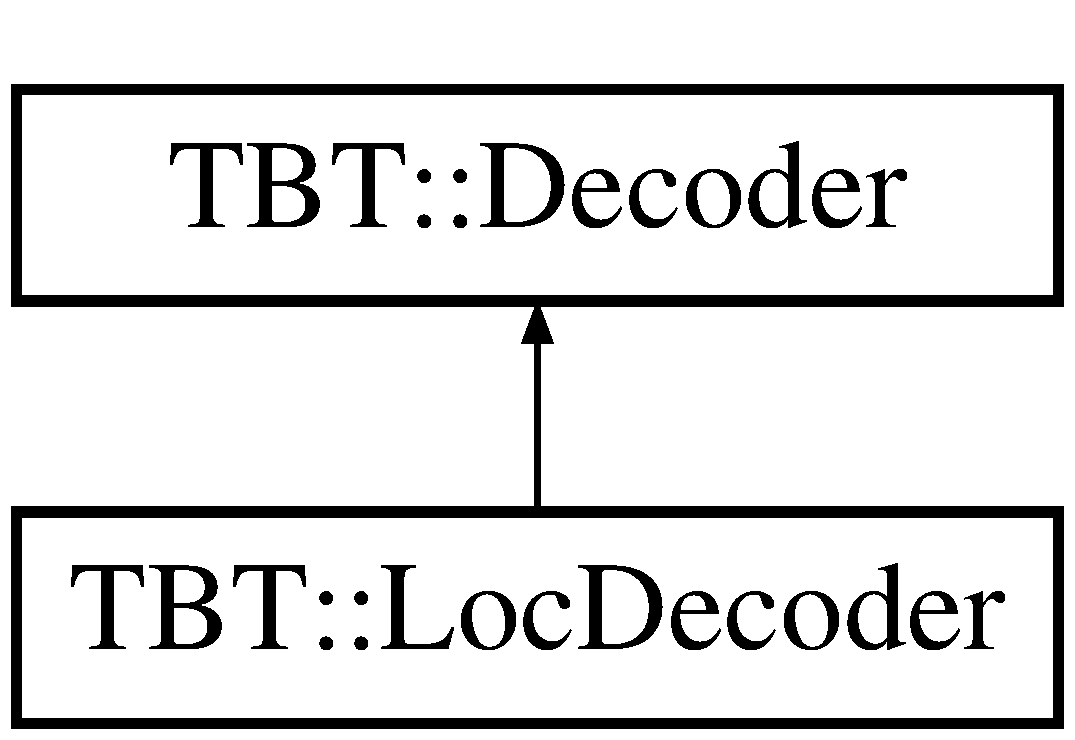
\includegraphics[height=2.000000cm]{classTBT_1_1Decoder}
\end{center}
\end{figure}
\subsection*{Public Member Functions}
\begin{DoxyCompactItemize}
\item 
\mbox{\Hypertarget{classTBT_1_1Decoder_a69cc50cb8ca993a98802303b1c70eade}\label{classTBT_1_1Decoder_a69cc50cb8ca993a98802303b1c70eade}} 
{\bfseries Decoder} (\hyperlink{classTBT_1_1Manager}{Manager} $\ast$p\+Manager, uint16\+\_\+t dcc\+Address)
\item 
\mbox{\Hypertarget{classTBT_1_1Decoder_ad948e489ff1246effdfda3e68d693593}\label{classTBT_1_1Decoder_ad948e489ff1246effdfda3e68d693593}} 
const uint16\+\_\+t {\bfseries get\+D\+C\+C\+Address} (void)
\item 
\mbox{\Hypertarget{classTBT_1_1Decoder_a71c25cd52e7f591ba1771ee0518735ba}\label{classTBT_1_1Decoder_a71c25cd52e7f591ba1771ee0518735ba}} 
virtual bool {\bfseries get\+Dcc\+Message} (uint8\+\_\+t $\ast$p\+Msg)
\end{DoxyCompactItemize}
\subsection*{Protected Attributes}
\begin{DoxyCompactItemize}
\item 
\mbox{\Hypertarget{classTBT_1_1Decoder_a14309179167dd46b722982301d651c4d}\label{classTBT_1_1Decoder_a14309179167dd46b722982301d651c4d}} 
uint16\+\_\+t {\bfseries m\+\_\+\+D\+C\+C\+Address}
\item 
\mbox{\Hypertarget{classTBT_1_1Decoder_a400475d21ba933f8b91e6f7d3053518b}\label{classTBT_1_1Decoder_a400475d21ba933f8b91e6f7d3053518b}} 
\hyperlink{classTBT_1_1Manager}{Manager} $\ast$ {\bfseries m\+\_\+p\+Manager}
\end{DoxyCompactItemize}


The documentation for this class was generated from the following files\+:\begin{DoxyCompactItemize}
\item 
Decoder.\+h\item 
Decoder.\+cpp\end{DoxyCompactItemize}

\hypertarget{classJson_1_1OurReader_1_1ErrorInfo}{}\section{Json\+:\+:Our\+Reader\+:\+:Error\+Info Class Reference}
\label{classJson_1_1OurReader_1_1ErrorInfo}\index{Json\+::\+Our\+Reader\+::\+Error\+Info@{Json\+::\+Our\+Reader\+::\+Error\+Info}}
\subsection*{Public Attributes}
\begin{DoxyCompactItemize}
\item 
\hyperlink{classJson_1_1OurReader_1_1Token}{Token} \hyperlink{classJson_1_1OurReader_1_1ErrorInfo_ad05204ecabe5e7201a842935b874ae9a_ad05204ecabe5e7201a842935b874ae9a}{token\+\_\+}
\item 
\hyperlink{json_8h_a1e723f95759de062585bc4a8fd3fa4be_a1e723f95759de062585bc4a8fd3fa4be}{J\+S\+O\+N\+C\+P\+P\+\_\+\+S\+T\+R\+I\+NG} \hyperlink{classJson_1_1OurReader_1_1ErrorInfo_af14b6bf58ee1cb3388c18ee336ee2394_af14b6bf58ee1cb3388c18ee336ee2394}{message\+\_\+}
\item 
\hyperlink{classJson_1_1OurReader_a1bdc7bbc52ba87cae6b19746f2ee0189_a1bdc7bbc52ba87cae6b19746f2ee0189}{Location} \hyperlink{classJson_1_1OurReader_1_1ErrorInfo_a77ba2d32a471c7b9bc14621b76a5bdab_a77ba2d32a471c7b9bc14621b76a5bdab}{extra\+\_\+}
\end{DoxyCompactItemize}


\subsection{Member Data Documentation}
\mbox{\Hypertarget{classJson_1_1OurReader_1_1ErrorInfo_a77ba2d32a471c7b9bc14621b76a5bdab_a77ba2d32a471c7b9bc14621b76a5bdab}\label{classJson_1_1OurReader_1_1ErrorInfo_a77ba2d32a471c7b9bc14621b76a5bdab_a77ba2d32a471c7b9bc14621b76a5bdab}} 
\index{Json\+::\+Our\+Reader\+::\+Error\+Info@{Json\+::\+Our\+Reader\+::\+Error\+Info}!extra\+\_\+@{extra\+\_\+}}
\index{extra\+\_\+@{extra\+\_\+}!Json\+::\+Our\+Reader\+::\+Error\+Info@{Json\+::\+Our\+Reader\+::\+Error\+Info}}
\subsubsection{\texorpdfstring{extra\+\_\+}{extra\_}}
{\footnotesize\ttfamily \hyperlink{classJson_1_1OurReader_a1bdc7bbc52ba87cae6b19746f2ee0189_a1bdc7bbc52ba87cae6b19746f2ee0189}{Location} Json\+::\+Our\+Reader\+::\+Error\+Info\+::extra\+\_\+}



Referenced by Json\+::\+Our\+Reader\+::add\+Error(), Json\+::\+Our\+Reader\+::get\+Formatted\+Error\+Messages(), and Json\+::\+Our\+Reader\+::push\+Error().

\mbox{\Hypertarget{classJson_1_1OurReader_1_1ErrorInfo_af14b6bf58ee1cb3388c18ee336ee2394_af14b6bf58ee1cb3388c18ee336ee2394}\label{classJson_1_1OurReader_1_1ErrorInfo_af14b6bf58ee1cb3388c18ee336ee2394_af14b6bf58ee1cb3388c18ee336ee2394}} 
\index{Json\+::\+Our\+Reader\+::\+Error\+Info@{Json\+::\+Our\+Reader\+::\+Error\+Info}!message\+\_\+@{message\+\_\+}}
\index{message\+\_\+@{message\+\_\+}!Json\+::\+Our\+Reader\+::\+Error\+Info@{Json\+::\+Our\+Reader\+::\+Error\+Info}}
\subsubsection{\texorpdfstring{message\+\_\+}{message\_}}
{\footnotesize\ttfamily \hyperlink{json_8h_a1e723f95759de062585bc4a8fd3fa4be_a1e723f95759de062585bc4a8fd3fa4be}{J\+S\+O\+N\+C\+P\+P\+\_\+\+S\+T\+R\+I\+NG} Json\+::\+Our\+Reader\+::\+Error\+Info\+::message\+\_\+}



Referenced by Json\+::\+Our\+Reader\+::add\+Error(), Json\+::\+Our\+Reader\+::get\+Formatted\+Error\+Messages(), Json\+::\+Our\+Reader\+::get\+Structured\+Errors(), and Json\+::\+Our\+Reader\+::push\+Error().

\mbox{\Hypertarget{classJson_1_1OurReader_1_1ErrorInfo_ad05204ecabe5e7201a842935b874ae9a_ad05204ecabe5e7201a842935b874ae9a}\label{classJson_1_1OurReader_1_1ErrorInfo_ad05204ecabe5e7201a842935b874ae9a_ad05204ecabe5e7201a842935b874ae9a}} 
\index{Json\+::\+Our\+Reader\+::\+Error\+Info@{Json\+::\+Our\+Reader\+::\+Error\+Info}!token\+\_\+@{token\+\_\+}}
\index{token\+\_\+@{token\+\_\+}!Json\+::\+Our\+Reader\+::\+Error\+Info@{Json\+::\+Our\+Reader\+::\+Error\+Info}}
\subsubsection{\texorpdfstring{token\+\_\+}{token\_}}
{\footnotesize\ttfamily \hyperlink{classJson_1_1OurReader_1_1Token}{Token} Json\+::\+Our\+Reader\+::\+Error\+Info\+::token\+\_\+}



Referenced by Json\+::\+Our\+Reader\+::add\+Error(), Json\+::\+Our\+Reader\+::get\+Formatted\+Error\+Messages(), Json\+::\+Our\+Reader\+::get\+Structured\+Errors(), and Json\+::\+Our\+Reader\+::push\+Error().



The documentation for this class was generated from the following file\+:\begin{DoxyCompactItemize}
\item 
\hyperlink{jsoncpp_8cpp}{jsoncpp.\+cpp}\end{DoxyCompactItemize}

\hypertarget{classJson_1_1Exception}{}\section{Json\+:\+:Exception Class Reference}
\label{classJson_1_1Exception}\index{Json\+::\+Exception@{Json\+::\+Exception}}


{\ttfamily \#include $<$json.\+h$>$}

Inheritance diagram for Json\+:\+:Exception\+:\begin{figure}[H]
\begin{center}
\leavevmode
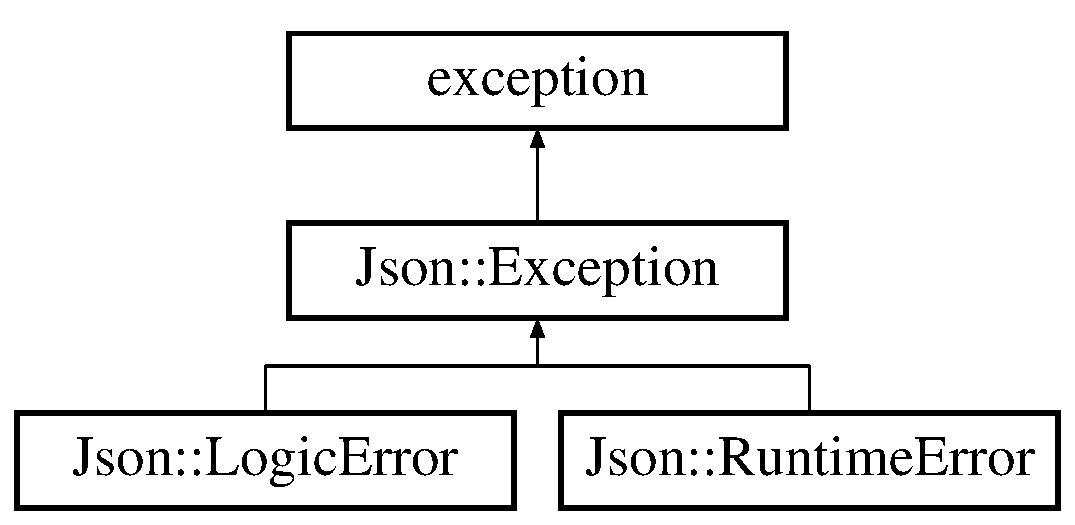
\includegraphics[height=3.000000cm]{classJson_1_1Exception}
\end{center}
\end{figure}
\subsection*{Public Member Functions}
\begin{DoxyCompactItemize}
\item 
\hyperlink{classJson_1_1Exception_ae764aa42e0755bd4ce9d303e2733fa8f_ae764aa42e0755bd4ce9d303e2733fa8f}{Exception} (\hyperlink{json_8h_a1e723f95759de062585bc4a8fd3fa4be_a1e723f95759de062585bc4a8fd3fa4be}{J\+S\+O\+N\+C\+P\+P\+\_\+\+S\+T\+R\+I\+NG} const \&msg)
\item 
\hyperlink{classJson_1_1Exception_add6af5e0ecdf36f40d7f3554b9786e21_add6af5e0ecdf36f40d7f3554b9786e21}{$\sim$\+Exception} () \hyperlink{json_8h_af8418c6d82d9de6e5f3c739fcf2fe88d_af8418c6d82d9de6e5f3c739fcf2fe88d}{J\+S\+O\+N\+C\+P\+P\+\_\+\+N\+O\+E\+X\+C\+E\+PT} \hyperlink{json_8h_a824d6199c91488107e443226fa6022c5_a824d6199c91488107e443226fa6022c5}{J\+S\+O\+N\+C\+P\+P\+\_\+\+O\+V\+E\+R\+R\+I\+DE}
\item 
char const  $\ast$ \hyperlink{classJson_1_1Exception_a70b7ce35e761fb93e8cd338e04619cd6_a70b7ce35e761fb93e8cd338e04619cd6}{what} () const \hyperlink{json_8h_af8418c6d82d9de6e5f3c739fcf2fe88d_af8418c6d82d9de6e5f3c739fcf2fe88d}{J\+S\+O\+N\+C\+P\+P\+\_\+\+N\+O\+E\+X\+C\+E\+PT} \hyperlink{json_8h_a824d6199c91488107e443226fa6022c5_a824d6199c91488107e443226fa6022c5}{J\+S\+O\+N\+C\+P\+P\+\_\+\+O\+V\+E\+R\+R\+I\+DE}
\end{DoxyCompactItemize}
\subsection*{Protected Attributes}
\begin{DoxyCompactItemize}
\item 
\hyperlink{json_8h_a1e723f95759de062585bc4a8fd3fa4be_a1e723f95759de062585bc4a8fd3fa4be}{J\+S\+O\+N\+C\+P\+P\+\_\+\+S\+T\+R\+I\+NG} \hyperlink{classJson_1_1Exception_aae3cbb8b45bf21480f64502a8329659f_aae3cbb8b45bf21480f64502a8329659f}{msg\+\_\+}
\end{DoxyCompactItemize}


\subsection{Detailed Description}
Base class for all exceptions we throw.

We use nothing but these internally. Of course, S\+TL can throw others. 

\subsection{Constructor \& Destructor Documentation}
\mbox{\Hypertarget{classJson_1_1Exception_ae764aa42e0755bd4ce9d303e2733fa8f_ae764aa42e0755bd4ce9d303e2733fa8f}\label{classJson_1_1Exception_ae764aa42e0755bd4ce9d303e2733fa8f_ae764aa42e0755bd4ce9d303e2733fa8f}} 
\index{Json\+::\+Exception@{Json\+::\+Exception}!Exception@{Exception}}
\index{Exception@{Exception}!Json\+::\+Exception@{Json\+::\+Exception}}
\subsubsection{\texorpdfstring{Exception()}{Exception()}}
{\footnotesize\ttfamily Json\+::\+Exception\+::\+Exception (\begin{DoxyParamCaption}\item[{\hyperlink{json_8h_a1e723f95759de062585bc4a8fd3fa4be_a1e723f95759de062585bc4a8fd3fa4be}{J\+S\+O\+N\+C\+P\+P\+\_\+\+S\+T\+R\+I\+NG} const \&}]{msg }\end{DoxyParamCaption})}

\mbox{\Hypertarget{classJson_1_1Exception_add6af5e0ecdf36f40d7f3554b9786e21_add6af5e0ecdf36f40d7f3554b9786e21}\label{classJson_1_1Exception_add6af5e0ecdf36f40d7f3554b9786e21_add6af5e0ecdf36f40d7f3554b9786e21}} 
\index{Json\+::\+Exception@{Json\+::\+Exception}!````~Exception@{$\sim$\+Exception}}
\index{````~Exception@{$\sim$\+Exception}!Json\+::\+Exception@{Json\+::\+Exception}}
\subsubsection{\texorpdfstring{$\sim$\+Exception()}{~Exception()}}
{\footnotesize\ttfamily Json\+::\+Exception\+::$\sim$\+Exception (\begin{DoxyParamCaption}{ }\end{DoxyParamCaption})}



\subsection{Member Function Documentation}
\mbox{\Hypertarget{classJson_1_1Exception_a70b7ce35e761fb93e8cd338e04619cd6_a70b7ce35e761fb93e8cd338e04619cd6}\label{classJson_1_1Exception_a70b7ce35e761fb93e8cd338e04619cd6_a70b7ce35e761fb93e8cd338e04619cd6}} 
\index{Json\+::\+Exception@{Json\+::\+Exception}!what@{what}}
\index{what@{what}!Json\+::\+Exception@{Json\+::\+Exception}}
\subsubsection{\texorpdfstring{what()}{what()}}
{\footnotesize\ttfamily char const  $\ast$ Json\+::\+Exception\+::what (\begin{DoxyParamCaption}{ }\end{DoxyParamCaption}) const}



References msg\+\_\+.



\subsection{Member Data Documentation}
\mbox{\Hypertarget{classJson_1_1Exception_aae3cbb8b45bf21480f64502a8329659f_aae3cbb8b45bf21480f64502a8329659f}\label{classJson_1_1Exception_aae3cbb8b45bf21480f64502a8329659f_aae3cbb8b45bf21480f64502a8329659f}} 
\index{Json\+::\+Exception@{Json\+::\+Exception}!msg\+\_\+@{msg\+\_\+}}
\index{msg\+\_\+@{msg\+\_\+}!Json\+::\+Exception@{Json\+::\+Exception}}
\subsubsection{\texorpdfstring{msg\+\_\+}{msg\_}}
{\footnotesize\ttfamily \hyperlink{json_8h_a1e723f95759de062585bc4a8fd3fa4be_a1e723f95759de062585bc4a8fd3fa4be}{J\+S\+O\+N\+C\+P\+P\+\_\+\+S\+T\+R\+I\+NG} Json\+::\+Exception\+::msg\+\_\+\hspace{0.3cm}{\ttfamily [protected]}}



Referenced by what().



The documentation for this class was generated from the following files\+:\begin{DoxyCompactItemize}
\item 
json/\hyperlink{json_8h}{json.\+h}\item 
\hyperlink{jsoncpp_8cpp}{jsoncpp.\+cpp}\end{DoxyCompactItemize}

\hypertarget{classJson_1_1CharReader_1_1Factory}{}\section{Json\+:\+:Char\+Reader\+:\+:Factory Class Reference}
\label{classJson_1_1CharReader_1_1Factory}\index{Json\+::\+Char\+Reader\+::\+Factory@{Json\+::\+Char\+Reader\+::\+Factory}}


{\ttfamily \#include $<$json.\+h$>$}

Inheritance diagram for Json\+:\+:Char\+Reader\+:\+:Factory\+:\begin{figure}[H]
\begin{center}
\leavevmode
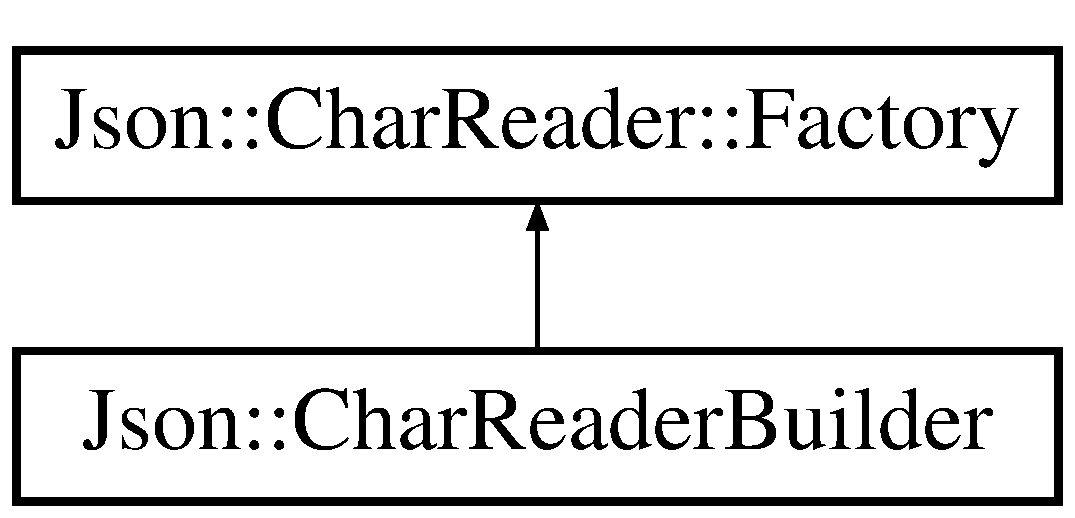
\includegraphics[height=2.000000cm]{classJson_1_1CharReader_1_1Factory}
\end{center}
\end{figure}
\subsection*{Public Member Functions}
\begin{DoxyCompactItemize}
\item 
virtual \hyperlink{classJson_1_1CharReader_1_1Factory_ae6938f632fa57f88e05818add5bc21be_ae6938f632fa57f88e05818add5bc21be}{$\sim$\+Factory} ()
\item 
virtual \hyperlink{classJson_1_1CharReader}{Char\+Reader} $\ast$ \hyperlink{classJson_1_1CharReader_1_1Factory_a4c5862a1ffd432372dbe65cf59de98c4_a4c5862a1ffd432372dbe65cf59de98c4}{new\+Char\+Reader} () const =0
\begin{DoxyCompactList}\small\item\em Allocate a \hyperlink{classJson_1_1CharReader}{Char\+Reader} via operator new(). \end{DoxyCompactList}\end{DoxyCompactItemize}


\subsection{Constructor \& Destructor Documentation}
\mbox{\Hypertarget{classJson_1_1CharReader_1_1Factory_ae6938f632fa57f88e05818add5bc21be_ae6938f632fa57f88e05818add5bc21be}\label{classJson_1_1CharReader_1_1Factory_ae6938f632fa57f88e05818add5bc21be_ae6938f632fa57f88e05818add5bc21be}} 
\index{Json\+::\+Char\+Reader\+::\+Factory@{Json\+::\+Char\+Reader\+::\+Factory}!````~Factory@{$\sim$\+Factory}}
\index{````~Factory@{$\sim$\+Factory}!Json\+::\+Char\+Reader\+::\+Factory@{Json\+::\+Char\+Reader\+::\+Factory}}
\subsubsection{\texorpdfstring{$\sim$\+Factory()}{~Factory()}}
{\footnotesize\ttfamily virtual Json\+::\+Char\+Reader\+::\+Factory\+::$\sim$\+Factory (\begin{DoxyParamCaption}{ }\end{DoxyParamCaption})\hspace{0.3cm}{\ttfamily [inline]}, {\ttfamily [virtual]}}



\subsection{Member Function Documentation}
\mbox{\Hypertarget{classJson_1_1CharReader_1_1Factory_a4c5862a1ffd432372dbe65cf59de98c4_a4c5862a1ffd432372dbe65cf59de98c4}\label{classJson_1_1CharReader_1_1Factory_a4c5862a1ffd432372dbe65cf59de98c4_a4c5862a1ffd432372dbe65cf59de98c4}} 
\index{Json\+::\+Char\+Reader\+::\+Factory@{Json\+::\+Char\+Reader\+::\+Factory}!new\+Char\+Reader@{new\+Char\+Reader}}
\index{new\+Char\+Reader@{new\+Char\+Reader}!Json\+::\+Char\+Reader\+::\+Factory@{Json\+::\+Char\+Reader\+::\+Factory}}
\subsubsection{\texorpdfstring{new\+Char\+Reader()}{newCharReader()}}
{\footnotesize\ttfamily virtual \hyperlink{classJson_1_1CharReader}{Char\+Reader}$\ast$ Json\+::\+Char\+Reader\+::\+Factory\+::new\+Char\+Reader (\begin{DoxyParamCaption}{ }\end{DoxyParamCaption}) const\hspace{0.3cm}{\ttfamily [pure virtual]}}



Allocate a \hyperlink{classJson_1_1CharReader}{Char\+Reader} via operator new(). 


\begin{DoxyExceptions}{Exceptions}
{\em std\+::exception} & if something goes wrong (e.\+g. invalid settings) \\
\hline
\end{DoxyExceptions}


Implemented in \hyperlink{classJson_1_1CharReaderBuilder_a3a262fcc76c1eb8eebfd4718fb4e9722_a3a262fcc76c1eb8eebfd4718fb4e9722}{Json\+::\+Char\+Reader\+Builder}.



Referenced by Json\+::parse\+From\+Stream().



The documentation for this class was generated from the following file\+:\begin{DoxyCompactItemize}
\item 
json/\hyperlink{json_8h}{json.\+h}\end{DoxyCompactItemize}

\hypertarget{classJson_1_1StreamWriter_1_1Factory}{}\section{Json\+:\+:Stream\+Writer\+:\+:Factory Class Reference}
\label{classJson_1_1StreamWriter_1_1Factory}\index{Json\+::\+Stream\+Writer\+::\+Factory@{Json\+::\+Stream\+Writer\+::\+Factory}}


A simple abstract factory.  




{\ttfamily \#include $<$json.\+h$>$}

Inheritance diagram for Json\+:\+:Stream\+Writer\+:\+:Factory\+:\begin{figure}[H]
\begin{center}
\leavevmode
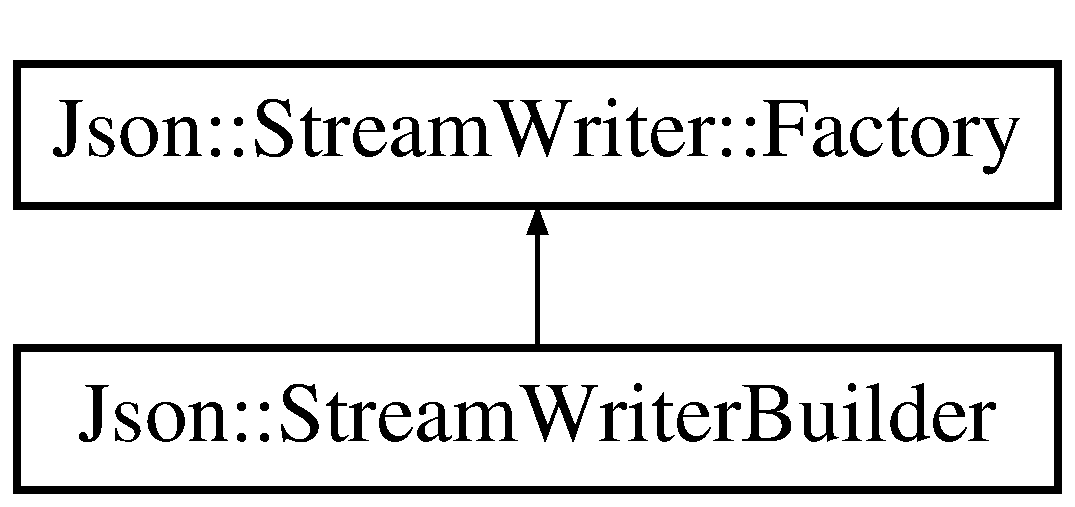
\includegraphics[height=2.000000cm]{classJson_1_1StreamWriter_1_1Factory}
\end{center}
\end{figure}
\subsection*{Public Member Functions}
\begin{DoxyCompactItemize}
\item 
virtual \hyperlink{classJson_1_1StreamWriter_1_1Factory_ad334ad5e81e3b9b1768620a446366ff1_ad334ad5e81e3b9b1768620a446366ff1}{$\sim$\+Factory} ()
\item 
virtual \hyperlink{classJson_1_1StreamWriter}{Stream\+Writer} $\ast$ \hyperlink{classJson_1_1StreamWriter_1_1Factory_a9d30ec53e8288cd53befccf1009c5f31_a9d30ec53e8288cd53befccf1009c5f31}{new\+Stream\+Writer} () const =0
\begin{DoxyCompactList}\small\item\em Allocate a \hyperlink{classJson_1_1CharReader}{Char\+Reader} via operator new(). \end{DoxyCompactList}\end{DoxyCompactItemize}


\subsection{Detailed Description}
A simple abstract factory. 

\subsection{Constructor \& Destructor Documentation}
\mbox{\Hypertarget{classJson_1_1StreamWriter_1_1Factory_ad334ad5e81e3b9b1768620a446366ff1_ad334ad5e81e3b9b1768620a446366ff1}\label{classJson_1_1StreamWriter_1_1Factory_ad334ad5e81e3b9b1768620a446366ff1_ad334ad5e81e3b9b1768620a446366ff1}} 
\index{Json\+::\+Stream\+Writer\+::\+Factory@{Json\+::\+Stream\+Writer\+::\+Factory}!````~Factory@{$\sim$\+Factory}}
\index{````~Factory@{$\sim$\+Factory}!Json\+::\+Stream\+Writer\+::\+Factory@{Json\+::\+Stream\+Writer\+::\+Factory}}
\subsubsection{\texorpdfstring{$\sim$\+Factory()}{~Factory()}}
{\footnotesize\ttfamily Json\+::\+Stream\+Writer\+::\+Factory\+::$\sim$\+Factory (\begin{DoxyParamCaption}{ }\end{DoxyParamCaption})\hspace{0.3cm}{\ttfamily [virtual]}}



\subsection{Member Function Documentation}
\mbox{\Hypertarget{classJson_1_1StreamWriter_1_1Factory_a9d30ec53e8288cd53befccf1009c5f31_a9d30ec53e8288cd53befccf1009c5f31}\label{classJson_1_1StreamWriter_1_1Factory_a9d30ec53e8288cd53befccf1009c5f31_a9d30ec53e8288cd53befccf1009c5f31}} 
\index{Json\+::\+Stream\+Writer\+::\+Factory@{Json\+::\+Stream\+Writer\+::\+Factory}!new\+Stream\+Writer@{new\+Stream\+Writer}}
\index{new\+Stream\+Writer@{new\+Stream\+Writer}!Json\+::\+Stream\+Writer\+::\+Factory@{Json\+::\+Stream\+Writer\+::\+Factory}}
\subsubsection{\texorpdfstring{new\+Stream\+Writer()}{newStreamWriter()}}
{\footnotesize\ttfamily virtual \hyperlink{classJson_1_1StreamWriter}{Stream\+Writer}$\ast$ Json\+::\+Stream\+Writer\+::\+Factory\+::new\+Stream\+Writer (\begin{DoxyParamCaption}{ }\end{DoxyParamCaption}) const\hspace{0.3cm}{\ttfamily [pure virtual]}}



Allocate a \hyperlink{classJson_1_1CharReader}{Char\+Reader} via operator new(). 


\begin{DoxyExceptions}{Exceptions}
{\em std\+::exception} & if something goes wrong (e.\+g. invalid settings) \\
\hline
\end{DoxyExceptions}


Implemented in \hyperlink{classJson_1_1StreamWriterBuilder_ab9ee278609f88ae04a7c1a84e1f559e6_ab9ee278609f88ae04a7c1a84e1f559e6}{Json\+::\+Stream\+Writer\+Builder}.



Referenced by Json\+::write\+String().



The documentation for this class was generated from the following files\+:\begin{DoxyCompactItemize}
\item 
json/\hyperlink{json_8h}{json.\+h}\item 
\hyperlink{jsoncpp_8cpp}{jsoncpp.\+cpp}\end{DoxyCompactItemize}

\hypertarget{classJson_1_1Features}{}\section{Json\+:\+:Features Class Reference}
\label{classJson_1_1Features}\index{Json\+::\+Features@{Json\+::\+Features}}


Configuration passed to reader and writer. This configuration object can be used to force the Reader or Writer to behave in a standard conforming way.  




{\ttfamily \#include $<$json.\+h$>$}

\subsection*{Public Member Functions}
\begin{DoxyCompactItemize}
\item 
\hyperlink{classJson_1_1Features_ad15a091cb61bb31323299a95970d2644_ad15a091cb61bb31323299a95970d2644}{Features} ()
\begin{DoxyCompactList}\small\item\em Initialize the configuration like Json\+Config\+::all\+Features;. \end{DoxyCompactList}\end{DoxyCompactItemize}
\subsection*{Static Public Member Functions}
\begin{DoxyCompactItemize}
\item 
static \hyperlink{classJson_1_1Features}{Features} \hyperlink{classJson_1_1Features_a63894da6e2c100b38741fa933f3d33ae_a63894da6e2c100b38741fa933f3d33ae}{all} ()
\begin{DoxyCompactList}\small\item\em A configuration that allows all features and assumes all strings are U\+T\+F-\/8. \end{DoxyCompactList}\item 
static \hyperlink{classJson_1_1Features}{Features} \hyperlink{classJson_1_1Features_ae23176c14b2e79e81fb61fb1a8ab58ee_ae23176c14b2e79e81fb61fb1a8ab58ee}{strict\+Mode} ()
\begin{DoxyCompactList}\small\item\em A configuration that is strictly compatible with the J\+S\+ON specification. \end{DoxyCompactList}\end{DoxyCompactItemize}
\subsection*{Public Attributes}
\begin{DoxyCompactItemize}
\item 
bool \hyperlink{classJson_1_1Features_a33afd389719624b6bdb23950b3c346c9_a33afd389719624b6bdb23950b3c346c9}{allow\+Comments\+\_\+}
\begin{DoxyCompactList}\small\item\em {\ttfamily true} if comments are allowed. Default\+: {\ttfamily true}. \end{DoxyCompactList}\item 
bool \hyperlink{classJson_1_1Features_a1162c37a1458adc32582b585b552f9c3_a1162c37a1458adc32582b585b552f9c3}{strict\+Root\+\_\+}
\item 
bool \hyperlink{classJson_1_1Features_a5076aa72c05c7596ac339ede36c97a6a_a5076aa72c05c7596ac339ede36c97a6a}{allow\+Dropped\+Null\+Placeholders\+\_\+}
\begin{DoxyCompactList}\small\item\em {\ttfamily true} if dropped null placeholders are allowed. Default\+: {\ttfamily false}. \end{DoxyCompactList}\item 
bool \hyperlink{classJson_1_1Features_aff3cb16b79d15d3d761b11a0dd6d4d6b_aff3cb16b79d15d3d761b11a0dd6d4d6b}{allow\+Numeric\+Keys\+\_\+}
\begin{DoxyCompactList}\small\item\em {\ttfamily true} if numeric object key are allowed. Default\+: {\ttfamily false}. \end{DoxyCompactList}\end{DoxyCompactItemize}


\subsection{Detailed Description}
Configuration passed to reader and writer. This configuration object can be used to force the Reader or Writer to behave in a standard conforming way. 

\subsection{Constructor \& Destructor Documentation}
\mbox{\Hypertarget{classJson_1_1Features_ad15a091cb61bb31323299a95970d2644_ad15a091cb61bb31323299a95970d2644}\label{classJson_1_1Features_ad15a091cb61bb31323299a95970d2644_ad15a091cb61bb31323299a95970d2644}} 
\index{Json\+::\+Features@{Json\+::\+Features}!Features@{Features}}
\index{Features@{Features}!Json\+::\+Features@{Json\+::\+Features}}
\subsubsection{\texorpdfstring{Features()}{Features()}}
{\footnotesize\ttfamily Json\+::\+Features\+::\+Features (\begin{DoxyParamCaption}{ }\end{DoxyParamCaption})}



Initialize the configuration like Json\+Config\+::all\+Features;. 



Referenced by all().



\subsection{Member Function Documentation}
\mbox{\Hypertarget{classJson_1_1Features_a63894da6e2c100b38741fa933f3d33ae_a63894da6e2c100b38741fa933f3d33ae}\label{classJson_1_1Features_a63894da6e2c100b38741fa933f3d33ae_a63894da6e2c100b38741fa933f3d33ae}} 
\index{Json\+::\+Features@{Json\+::\+Features}!all@{all}}
\index{all@{all}!Json\+::\+Features@{Json\+::\+Features}}
\subsubsection{\texorpdfstring{all()}{all()}}
{\footnotesize\ttfamily \hyperlink{classJson_1_1Features}{Features} Json\+::\+Features\+::all (\begin{DoxyParamCaption}{ }\end{DoxyParamCaption})\hspace{0.3cm}{\ttfamily [static]}}



A configuration that allows all features and assumes all strings are U\+T\+F-\/8. 


\begin{DoxyItemize}
\item C \& C++ comments are allowed
\item Root object can be any J\+S\+ON value
\item Assumes \hyperlink{classJson_1_1Value}{Value} strings are encoded in U\+T\+F-\/8 
\end{DoxyItemize}

References Features().



Referenced by strict\+Mode().

\mbox{\Hypertarget{classJson_1_1Features_ae23176c14b2e79e81fb61fb1a8ab58ee_ae23176c14b2e79e81fb61fb1a8ab58ee}\label{classJson_1_1Features_ae23176c14b2e79e81fb61fb1a8ab58ee_ae23176c14b2e79e81fb61fb1a8ab58ee}} 
\index{Json\+::\+Features@{Json\+::\+Features}!strict\+Mode@{strict\+Mode}}
\index{strict\+Mode@{strict\+Mode}!Json\+::\+Features@{Json\+::\+Features}}
\subsubsection{\texorpdfstring{strict\+Mode()}{strictMode()}}
{\footnotesize\ttfamily \hyperlink{classJson_1_1Features}{Features} Json\+::\+Features\+::strict\+Mode (\begin{DoxyParamCaption}{ }\end{DoxyParamCaption})\hspace{0.3cm}{\ttfamily [static]}}



A configuration that is strictly compatible with the J\+S\+ON specification. 


\begin{DoxyItemize}
\item Comments are forbidden.
\item Root object must be either an array or an object value.
\item Assumes \hyperlink{classJson_1_1Value}{Value} strings are encoded in U\+T\+F-\/8 
\end{DoxyItemize}

References all(), allow\+Comments\+\_\+, allow\+Dropped\+Null\+Placeholders\+\_\+, allow\+Numeric\+Keys\+\_\+, Json\+::array\+Value, Json\+::\+Value\+::as\+C\+String(), Json\+::code\+Point\+To\+U\+T\+F8(), Json\+::comment\+After, Json\+::comment\+After\+On\+Same\+Line, Json\+::comment\+Before, Json\+::\+Value\+::get\+Offset\+Limit(), Json\+::\+Value\+::get\+Offset\+Start(), Json\+::\+Value\+::is\+Array(), Json\+::\+Value\+::is\+Object(), J\+S\+O\+N\+C\+P\+P\+\_\+\+I\+S\+T\+R\+I\+N\+G\+S\+T\+R\+E\+AM, J\+S\+O\+N\+C\+P\+P\+\_\+\+S\+T\+R\+I\+NG, Json\+::\+Value\+::max\+Int, Json\+::\+Value\+::max\+Largest\+Int, Json\+::\+Value\+::max\+Largest\+U\+Int, Json\+::\+Value\+::min\+Largest\+Int, Json\+::object\+Value, Json\+::\+Value\+::set\+Comment(), stack\+Limit\+\_\+g, strict\+Root\+\_\+, Json\+::\+Value\+::swap\+Payload(), and Json\+::throw\+Runtime\+Error().



\subsection{Member Data Documentation}
\mbox{\Hypertarget{classJson_1_1Features_a33afd389719624b6bdb23950b3c346c9_a33afd389719624b6bdb23950b3c346c9}\label{classJson_1_1Features_a33afd389719624b6bdb23950b3c346c9_a33afd389719624b6bdb23950b3c346c9}} 
\index{Json\+::\+Features@{Json\+::\+Features}!allow\+Comments\+\_\+@{allow\+Comments\+\_\+}}
\index{allow\+Comments\+\_\+@{allow\+Comments\+\_\+}!Json\+::\+Features@{Json\+::\+Features}}
\subsubsection{\texorpdfstring{allow\+Comments\+\_\+}{allowComments\_}}
{\footnotesize\ttfamily bool Json\+::\+Features\+::allow\+Comments\+\_\+}



{\ttfamily true} if comments are allowed. Default\+: {\ttfamily true}. 



Referenced by strict\+Mode().

\mbox{\Hypertarget{classJson_1_1Features_a5076aa72c05c7596ac339ede36c97a6a_a5076aa72c05c7596ac339ede36c97a6a}\label{classJson_1_1Features_a5076aa72c05c7596ac339ede36c97a6a_a5076aa72c05c7596ac339ede36c97a6a}} 
\index{Json\+::\+Features@{Json\+::\+Features}!allow\+Dropped\+Null\+Placeholders\+\_\+@{allow\+Dropped\+Null\+Placeholders\+\_\+}}
\index{allow\+Dropped\+Null\+Placeholders\+\_\+@{allow\+Dropped\+Null\+Placeholders\+\_\+}!Json\+::\+Features@{Json\+::\+Features}}
\subsubsection{\texorpdfstring{allow\+Dropped\+Null\+Placeholders\+\_\+}{allowDroppedNullPlaceholders\_}}
{\footnotesize\ttfamily bool Json\+::\+Features\+::allow\+Dropped\+Null\+Placeholders\+\_\+}



{\ttfamily true} if dropped null placeholders are allowed. Default\+: {\ttfamily false}. 



Referenced by strict\+Mode().

\mbox{\Hypertarget{classJson_1_1Features_aff3cb16b79d15d3d761b11a0dd6d4d6b_aff3cb16b79d15d3d761b11a0dd6d4d6b}\label{classJson_1_1Features_aff3cb16b79d15d3d761b11a0dd6d4d6b_aff3cb16b79d15d3d761b11a0dd6d4d6b}} 
\index{Json\+::\+Features@{Json\+::\+Features}!allow\+Numeric\+Keys\+\_\+@{allow\+Numeric\+Keys\+\_\+}}
\index{allow\+Numeric\+Keys\+\_\+@{allow\+Numeric\+Keys\+\_\+}!Json\+::\+Features@{Json\+::\+Features}}
\subsubsection{\texorpdfstring{allow\+Numeric\+Keys\+\_\+}{allowNumericKeys\_}}
{\footnotesize\ttfamily bool Json\+::\+Features\+::allow\+Numeric\+Keys\+\_\+}



{\ttfamily true} if numeric object key are allowed. Default\+: {\ttfamily false}. 



Referenced by strict\+Mode().

\mbox{\Hypertarget{classJson_1_1Features_a1162c37a1458adc32582b585b552f9c3_a1162c37a1458adc32582b585b552f9c3}\label{classJson_1_1Features_a1162c37a1458adc32582b585b552f9c3_a1162c37a1458adc32582b585b552f9c3}} 
\index{Json\+::\+Features@{Json\+::\+Features}!strict\+Root\+\_\+@{strict\+Root\+\_\+}}
\index{strict\+Root\+\_\+@{strict\+Root\+\_\+}!Json\+::\+Features@{Json\+::\+Features}}
\subsubsection{\texorpdfstring{strict\+Root\+\_\+}{strictRoot\_}}
{\footnotesize\ttfamily bool Json\+::\+Features\+::strict\+Root\+\_\+}

{\ttfamily true} if root must be either an array or an object value. Default\+: {\ttfamily false}. 

Referenced by strict\+Mode().



The documentation for this class was generated from the following files\+:\begin{DoxyCompactItemize}
\item 
json/\hyperlink{json_8h}{json.\+h}\item 
\hyperlink{jsoncpp_8cpp}{jsoncpp.\+cpp}\end{DoxyCompactItemize}

\hypertarget{structhttp__message}{}\section{http\+\_\+message Struct Reference}
\label{structhttp__message}\index{http\+\_\+message@{http\+\_\+message}}
\subsection*{Public Attributes}
\begin{DoxyCompactItemize}
\item 
\mbox{\Hypertarget{structhttp__message_a005f4310b3d6f7f2c818e4dff1c81d10}\label{structhttp__message_a005f4310b3d6f7f2c818e4dff1c81d10}} 
struct \hyperlink{structmg__str}{mg\+\_\+str} {\bfseries message}
\item 
\mbox{\Hypertarget{structhttp__message_ab2e0f6d6abe3879d9f85238ae9c10fd5}\label{structhttp__message_ab2e0f6d6abe3879d9f85238ae9c10fd5}} 
struct \hyperlink{structmg__str}{mg\+\_\+str} {\bfseries body}
\item 
\mbox{\Hypertarget{structhttp__message_a446deffe0f2da170fb9216fd5c8812d2}\label{structhttp__message_a446deffe0f2da170fb9216fd5c8812d2}} 
struct \hyperlink{structmg__str}{mg\+\_\+str} {\bfseries method}
\item 
\mbox{\Hypertarget{structhttp__message_a2f8d9e674965443571fd6e581393dd62}\label{structhttp__message_a2f8d9e674965443571fd6e581393dd62}} 
struct \hyperlink{structmg__str}{mg\+\_\+str} {\bfseries uri}
\item 
\mbox{\Hypertarget{structhttp__message_aafd1525884e7c83d781d86c063ec1f4f}\label{structhttp__message_aafd1525884e7c83d781d86c063ec1f4f}} 
struct \hyperlink{structmg__str}{mg\+\_\+str} {\bfseries proto}
\item 
\mbox{\Hypertarget{structhttp__message_a1c4e12c873f1e4d9711d470e2e32fa65}\label{structhttp__message_a1c4e12c873f1e4d9711d470e2e32fa65}} 
int {\bfseries resp\+\_\+code}
\item 
\mbox{\Hypertarget{structhttp__message_ae819bf6100f781e15515c01bf03f5a76}\label{structhttp__message_ae819bf6100f781e15515c01bf03f5a76}} 
struct \hyperlink{structmg__str}{mg\+\_\+str} {\bfseries resp\+\_\+status\+\_\+msg}
\item 
\mbox{\Hypertarget{structhttp__message_a899c4cefcdda3ba4fbafcfb05a85bba5}\label{structhttp__message_a899c4cefcdda3ba4fbafcfb05a85bba5}} 
struct \hyperlink{structmg__str}{mg\+\_\+str} {\bfseries query\+\_\+string}
\item 
\mbox{\Hypertarget{structhttp__message_ad0a1f9898353bfcc80ab7f2f0a22adb0}\label{structhttp__message_ad0a1f9898353bfcc80ab7f2f0a22adb0}} 
struct \hyperlink{structmg__str}{mg\+\_\+str} {\bfseries header\+\_\+names} \mbox{[}M\+G\+\_\+\+M\+A\+X\+\_\+\+H\+T\+T\+P\+\_\+\+H\+E\+A\+D\+E\+RS\mbox{]}
\item 
\mbox{\Hypertarget{structhttp__message_a95a0bfefd3a05bb3db52ce50a2ef71f4}\label{structhttp__message_a95a0bfefd3a05bb3db52ce50a2ef71f4}} 
struct \hyperlink{structmg__str}{mg\+\_\+str} {\bfseries header\+\_\+values} \mbox{[}M\+G\+\_\+\+M\+A\+X\+\_\+\+H\+T\+T\+P\+\_\+\+H\+E\+A\+D\+E\+RS\mbox{]}
\end{DoxyCompactItemize}


The documentation for this struct was generated from the following file\+:\begin{DoxyCompactItemize}
\item 
mongoose.\+h\end{DoxyCompactItemize}

\hypertarget{classTBT_1_1LocDecoder}{}\section{T\+BT\+:\+:Loc\+Decoder Class Reference}
\label{classTBT_1_1LocDecoder}\index{T\+B\+T\+::\+Loc\+Decoder@{T\+B\+T\+::\+Loc\+Decoder}}
Inheritance diagram for T\+BT\+:\+:Loc\+Decoder\+:\begin{figure}[H]
\begin{center}
\leavevmode
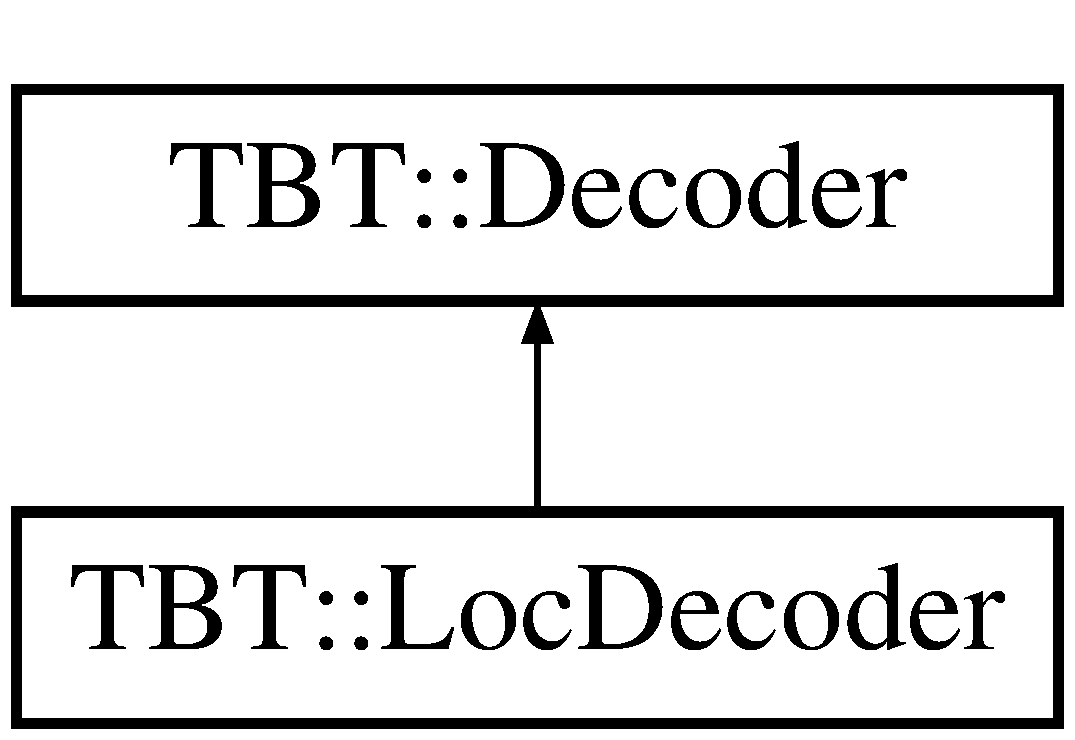
\includegraphics[height=2.000000cm]{classTBT_1_1LocDecoder}
\end{center}
\end{figure}
\subsection*{Public Member Functions}
\begin{DoxyCompactItemize}
\item 
\mbox{\Hypertarget{classTBT_1_1LocDecoder_ae8563de74c15f27c40644bf8218d26d9}\label{classTBT_1_1LocDecoder_ae8563de74c15f27c40644bf8218d26d9}} 
{\bfseries Loc\+Decoder} (\hyperlink{classTBT_1_1Manager}{Manager} $\ast$p\+Manager, uint16\+\_\+t dcc\+Address)
\item 
\mbox{\Hypertarget{classTBT_1_1LocDecoder_afaa04ad0561a39212d69d0aabece751e}\label{classTBT_1_1LocDecoder_afaa04ad0561a39212d69d0aabece751e}} 
uint8\+\_\+t {\bfseries get\+Loc\+Mode} (void)
\item 
\mbox{\Hypertarget{classTBT_1_1LocDecoder_a257c294961f07e5f2134b1550355a661}\label{classTBT_1_1LocDecoder_a257c294961f07e5f2134b1550355a661}} 
void {\bfseries get\+L\+A\+N\+Loc\+Info} (uint8\+\_\+t $\ast$p\+Msg)
\item 
\mbox{\Hypertarget{classTBT_1_1LocDecoder_a0ed2026cd64ba1e2aa411e1228027f4e}\label{classTBT_1_1LocDecoder_a0ed2026cd64ba1e2aa411e1228027f4e}} 
uint8\+\_\+t {\bfseries set\+Loc\+Mode} (uint8\+\_\+t new\+Mode)
\item 
\mbox{\Hypertarget{classTBT_1_1LocDecoder_a3ec11c7c270d1eeb00e6893bff8f0831}\label{classTBT_1_1LocDecoder_a3ec11c7c270d1eeb00e6893bff8f0831}} 
bool {\bfseries get\+Busy} ()
\item 
\mbox{\Hypertarget{classTBT_1_1LocDecoder_ae89a770202444bca60595182fe4a9c90}\label{classTBT_1_1LocDecoder_ae89a770202444bca60595182fe4a9c90}} 
uint8\+\_\+t {\bfseries get\+Speedsteps} ()
\item 
\mbox{\Hypertarget{classTBT_1_1LocDecoder_a5c570e65adde5ee526986155d509da47}\label{classTBT_1_1LocDecoder_a5c570e65adde5ee526986155d509da47}} 
bool {\bfseries get\+Direction} ()
\item 
\mbox{\Hypertarget{classTBT_1_1LocDecoder_a7305c8ab02a76b48b2b5ab93f1aec24b}\label{classTBT_1_1LocDecoder_a7305c8ab02a76b48b2b5ab93f1aec24b}} 
uint8\+\_\+t {\bfseries get\+Speed} ()
\item 
\mbox{\Hypertarget{classTBT_1_1LocDecoder_a7f4c04a5a306ea827494b29789cc401e}\label{classTBT_1_1LocDecoder_a7f4c04a5a306ea827494b29789cc401e}} 
bool {\bfseries get\+Dual\+Traction} ()
\item 
\mbox{\Hypertarget{classTBT_1_1LocDecoder_ab0a2b2953657fbc2589f90918883d03a}\label{classTBT_1_1LocDecoder_ab0a2b2953657fbc2589f90918883d03a}} 
bool {\bfseries get\+Smart\+Search} ()
\item 
\mbox{\Hypertarget{classTBT_1_1LocDecoder_a14a2d03a9f667ebfc4472fab880271b7}\label{classTBT_1_1LocDecoder_a14a2d03a9f667ebfc4472fab880271b7}} 
bool {\bfseries get\+Light} ()
\item 
\mbox{\Hypertarget{classTBT_1_1LocDecoder_ad659466bfea38d48902183acd6c450ab}\label{classTBT_1_1LocDecoder_ad659466bfea38d48902183acd6c450ab}} 
uint8\+\_\+t {\bfseries get\+Function\+Group1} ()
\item 
\mbox{\Hypertarget{classTBT_1_1LocDecoder_add8099fb79a671d02eeb993358f237fc}\label{classTBT_1_1LocDecoder_add8099fb79a671d02eeb993358f237fc}} 
bool {\bfseries get\+F0} ()
\item 
\mbox{\Hypertarget{classTBT_1_1LocDecoder_a583ff5f16d5b22d41be688b788f928bf}\label{classTBT_1_1LocDecoder_a583ff5f16d5b22d41be688b788f928bf}} 
bool {\bfseries get\+F1} ()
\item 
\mbox{\Hypertarget{classTBT_1_1LocDecoder_a1ed926bf58e50df8dd8650f268c26b6f}\label{classTBT_1_1LocDecoder_a1ed926bf58e50df8dd8650f268c26b6f}} 
bool {\bfseries get\+F2} ()
\item 
\mbox{\Hypertarget{classTBT_1_1LocDecoder_a421ae56808383dbc63de19b21c08fb5d}\label{classTBT_1_1LocDecoder_a421ae56808383dbc63de19b21c08fb5d}} 
bool {\bfseries get\+F3} ()
\item 
\mbox{\Hypertarget{classTBT_1_1LocDecoder_a2af90878d4f8f1f3b64f393519ac8f7a}\label{classTBT_1_1LocDecoder_a2af90878d4f8f1f3b64f393519ac8f7a}} 
bool {\bfseries get\+F4} ()
\item 
\mbox{\Hypertarget{classTBT_1_1LocDecoder_a5a23ba503d7b4798ac8c00019e4d3557}\label{classTBT_1_1LocDecoder_a5a23ba503d7b4798ac8c00019e4d3557}} 
uint8\+\_\+t {\bfseries get\+Function\+Group2} ()
\item 
\mbox{\Hypertarget{classTBT_1_1LocDecoder_a25b602fa8075cd6eb22bb936d9e957c7}\label{classTBT_1_1LocDecoder_a25b602fa8075cd6eb22bb936d9e957c7}} 
bool {\bfseries get\+F5} ()
\item 
\mbox{\Hypertarget{classTBT_1_1LocDecoder_a41b96104eec97905909c8c99c20756e5}\label{classTBT_1_1LocDecoder_a41b96104eec97905909c8c99c20756e5}} 
bool {\bfseries get\+F6} ()
\item 
\mbox{\Hypertarget{classTBT_1_1LocDecoder_a3f0a6c199b8222c53f047bd32f9060fc}\label{classTBT_1_1LocDecoder_a3f0a6c199b8222c53f047bd32f9060fc}} 
bool {\bfseries get\+F7} ()
\item 
\mbox{\Hypertarget{classTBT_1_1LocDecoder_ade02f20fc47f75a60a16f5f14339f7a1}\label{classTBT_1_1LocDecoder_ade02f20fc47f75a60a16f5f14339f7a1}} 
bool {\bfseries get\+F8} ()
\item 
\mbox{\Hypertarget{classTBT_1_1LocDecoder_a756c41f02751356fb934252b20c8b0f0}\label{classTBT_1_1LocDecoder_a756c41f02751356fb934252b20c8b0f0}} 
uint8\+\_\+t {\bfseries get\+Function\+Group3} ()
\item 
\mbox{\Hypertarget{classTBT_1_1LocDecoder_adfbe30b0ab41b8a126514938d98b3222}\label{classTBT_1_1LocDecoder_adfbe30b0ab41b8a126514938d98b3222}} 
bool {\bfseries get\+F9} ()
\item 
\mbox{\Hypertarget{classTBT_1_1LocDecoder_ac891adfab9ecf9ca3dec29d387698c30}\label{classTBT_1_1LocDecoder_ac891adfab9ecf9ca3dec29d387698c30}} 
bool {\bfseries get\+F10} ()
\item 
\mbox{\Hypertarget{classTBT_1_1LocDecoder_af3beee6516b8af8046b469d6326250b1}\label{classTBT_1_1LocDecoder_af3beee6516b8af8046b469d6326250b1}} 
bool {\bfseries get\+F11} ()
\item 
\mbox{\Hypertarget{classTBT_1_1LocDecoder_aa9ff3866964a5a6be01d6a6c22498b9d}\label{classTBT_1_1LocDecoder_aa9ff3866964a5a6be01d6a6c22498b9d}} 
bool {\bfseries get\+F12} ()
\item 
\mbox{\Hypertarget{classTBT_1_1LocDecoder_ab3f960f23613062dd97a3fb2274ee02c}\label{classTBT_1_1LocDecoder_ab3f960f23613062dd97a3fb2274ee02c}} 
uint8\+\_\+t {\bfseries get\+Function\+Group4} ()
\item 
\mbox{\Hypertarget{classTBT_1_1LocDecoder_aeca11289c531630bcecf39fd747d97b4}\label{classTBT_1_1LocDecoder_aeca11289c531630bcecf39fd747d97b4}} 
bool {\bfseries get\+F13} ()
\item 
\mbox{\Hypertarget{classTBT_1_1LocDecoder_a839308828d5775da64621292caa07651}\label{classTBT_1_1LocDecoder_a839308828d5775da64621292caa07651}} 
bool {\bfseries get\+F14} ()
\item 
\mbox{\Hypertarget{classTBT_1_1LocDecoder_a4bcfbf55ed042a80d5b045eb7915234a}\label{classTBT_1_1LocDecoder_a4bcfbf55ed042a80d5b045eb7915234a}} 
bool {\bfseries get\+F15} ()
\item 
\mbox{\Hypertarget{classTBT_1_1LocDecoder_a11aa0521314deb69fd50d44eb9f35d8d}\label{classTBT_1_1LocDecoder_a11aa0521314deb69fd50d44eb9f35d8d}} 
bool {\bfseries get\+F16} ()
\item 
\mbox{\Hypertarget{classTBT_1_1LocDecoder_a3197258036f35718c884aba8df521b54}\label{classTBT_1_1LocDecoder_a3197258036f35718c884aba8df521b54}} 
bool {\bfseries get\+F17} ()
\item 
\mbox{\Hypertarget{classTBT_1_1LocDecoder_a8a0533187d68e90e5a616dbcc934a111}\label{classTBT_1_1LocDecoder_a8a0533187d68e90e5a616dbcc934a111}} 
bool {\bfseries get\+F18} ()
\item 
\mbox{\Hypertarget{classTBT_1_1LocDecoder_ad61a122b7e69336f878baa2f5670a4e8}\label{classTBT_1_1LocDecoder_ad61a122b7e69336f878baa2f5670a4e8}} 
bool {\bfseries get\+F19} ()
\item 
\mbox{\Hypertarget{classTBT_1_1LocDecoder_abcb11e56a79e9229212139723630aef0}\label{classTBT_1_1LocDecoder_abcb11e56a79e9229212139723630aef0}} 
bool {\bfseries get\+F20} ()
\item 
\mbox{\Hypertarget{classTBT_1_1LocDecoder_aac83243e509961ce7eedb9959fcecb73}\label{classTBT_1_1LocDecoder_aac83243e509961ce7eedb9959fcecb73}} 
uint8\+\_\+t {\bfseries get\+Function\+Group5} ()
\item 
\mbox{\Hypertarget{classTBT_1_1LocDecoder_a89ea694d153a4f68ffe7df1f37fd7fc6}\label{classTBT_1_1LocDecoder_a89ea694d153a4f68ffe7df1f37fd7fc6}} 
bool {\bfseries get\+F21} ()
\item 
\mbox{\Hypertarget{classTBT_1_1LocDecoder_a9d95d2ac3b1079b9ffa519440808d4e2}\label{classTBT_1_1LocDecoder_a9d95d2ac3b1079b9ffa519440808d4e2}} 
bool {\bfseries get\+F22} ()
\item 
\mbox{\Hypertarget{classTBT_1_1LocDecoder_ab03cf89a7d635e61ebb1362f5f8274fc}\label{classTBT_1_1LocDecoder_ab03cf89a7d635e61ebb1362f5f8274fc}} 
bool {\bfseries get\+F23} ()
\item 
\mbox{\Hypertarget{classTBT_1_1LocDecoder_a16317eca85676a89372298782c71c6cb}\label{classTBT_1_1LocDecoder_a16317eca85676a89372298782c71c6cb}} 
bool {\bfseries get\+F24} ()
\item 
\mbox{\Hypertarget{classTBT_1_1LocDecoder_a3e06e61df29ee70660c003cbe81cb497}\label{classTBT_1_1LocDecoder_a3e06e61df29ee70660c003cbe81cb497}} 
bool {\bfseries get\+F25} ()
\item 
\mbox{\Hypertarget{classTBT_1_1LocDecoder_aa240dc8548525b91d931eed9cd549657}\label{classTBT_1_1LocDecoder_aa240dc8548525b91d931eed9cd549657}} 
bool {\bfseries get\+F26} ()
\item 
\mbox{\Hypertarget{classTBT_1_1LocDecoder_a0f8abd84b95094b2a139bd3402153aae}\label{classTBT_1_1LocDecoder_a0f8abd84b95094b2a139bd3402153aae}} 
bool {\bfseries get\+F27} ()
\item 
\mbox{\Hypertarget{classTBT_1_1LocDecoder_aecb2127b4edc17aac10dda93b4404e1d}\label{classTBT_1_1LocDecoder_aecb2127b4edc17aac10dda93b4404e1d}} 
bool {\bfseries get\+F28} ()
\item 
\mbox{\Hypertarget{classTBT_1_1LocDecoder_ac8f62e05b5ea28dcbaf1c07a1c4a91ec}\label{classTBT_1_1LocDecoder_ac8f62e05b5ea28dcbaf1c07a1c4a91ec}} 
void {\bfseries set\+Busy} (bool value)
\item 
\mbox{\Hypertarget{classTBT_1_1LocDecoder_aa919a313cb33a49d792694a544f2d3de}\label{classTBT_1_1LocDecoder_aa919a313cb33a49d792694a544f2d3de}} 
void {\bfseries set\+Speedsteps} (uint8\+\_\+t value)
\item 
\mbox{\Hypertarget{classTBT_1_1LocDecoder_a5b0ba8089edaf920fb513e26701580bf}\label{classTBT_1_1LocDecoder_a5b0ba8089edaf920fb513e26701580bf}} 
void {\bfseries set\+Loco\+Drive14} (uint8\+\_\+t value)
\item 
\mbox{\Hypertarget{classTBT_1_1LocDecoder_ace59dd8679514643328ce916057669e4}\label{classTBT_1_1LocDecoder_ace59dd8679514643328ce916057669e4}} 
void {\bfseries set\+Loco\+Drive27} (uint8\+\_\+t value)
\item 
\mbox{\Hypertarget{classTBT_1_1LocDecoder_a6bbf6c173217c49b7d4909b9c4cb5127}\label{classTBT_1_1LocDecoder_a6bbf6c173217c49b7d4909b9c4cb5127}} 
void {\bfseries set\+Loco\+Drive28} (uint8\+\_\+t value)
\item 
\mbox{\Hypertarget{classTBT_1_1LocDecoder_a9de246d419829f424e8b50c817c599ca}\label{classTBT_1_1LocDecoder_a9de246d419829f424e8b50c817c599ca}} 
void {\bfseries set\+Loco\+Drive128} (uint8\+\_\+t value)
\item 
\mbox{\Hypertarget{classTBT_1_1LocDecoder_a7e5a054cecfa15cc2574b166c2001deb}\label{classTBT_1_1LocDecoder_a7e5a054cecfa15cc2574b166c2001deb}} 
void {\bfseries set\+Direction} (bool value)
\item 
\mbox{\Hypertarget{classTBT_1_1LocDecoder_afa7b68a8e717065e39c80a83cbd9bb66}\label{classTBT_1_1LocDecoder_afa7b68a8e717065e39c80a83cbd9bb66}} 
void {\bfseries set\+Speed} (uint8\+\_\+t value)
\item 
\mbox{\Hypertarget{classTBT_1_1LocDecoder_a1dbc0fcca21619d0283e1a61bbb1f7b2}\label{classTBT_1_1LocDecoder_a1dbc0fcca21619d0283e1a61bbb1f7b2}} 
void {\bfseries set\+Dual\+Traction} (bool value)
\item 
\mbox{\Hypertarget{classTBT_1_1LocDecoder_ab17b176f9fb53af19911611dc35c4e76}\label{classTBT_1_1LocDecoder_ab17b176f9fb53af19911611dc35c4e76}} 
void {\bfseries set\+Smart\+Search} (bool value)
\item 
\mbox{\Hypertarget{classTBT_1_1LocDecoder_a7d77fa29a27f1abff7dba21c3cca7ff1}\label{classTBT_1_1LocDecoder_a7d77fa29a27f1abff7dba21c3cca7ff1}} 
void {\bfseries set\+Function\+Group1} (const uint8\+\_\+t \&value)
\item 
\mbox{\Hypertarget{classTBT_1_1LocDecoder_a71807a8bab2731cc511659f118ecb01a}\label{classTBT_1_1LocDecoder_a71807a8bab2731cc511659f118ecb01a}} 
void {\bfseries set\+Light} (bool value)
\item 
\mbox{\Hypertarget{classTBT_1_1LocDecoder_ae7dc2a2221ba08ecaf34f50636f59b54}\label{classTBT_1_1LocDecoder_ae7dc2a2221ba08ecaf34f50636f59b54}} 
void {\bfseries set\+F0} (bool value)
\item 
\mbox{\Hypertarget{classTBT_1_1LocDecoder_aba76c6a9b002224297ba04ded570eee4}\label{classTBT_1_1LocDecoder_aba76c6a9b002224297ba04ded570eee4}} 
void {\bfseries set\+F1} (bool value)
\item 
\mbox{\Hypertarget{classTBT_1_1LocDecoder_a60e4822d5d730abec02cf045353d5316}\label{classTBT_1_1LocDecoder_a60e4822d5d730abec02cf045353d5316}} 
void {\bfseries set\+F2} (bool value)
\item 
\mbox{\Hypertarget{classTBT_1_1LocDecoder_a6316b9510a9f3552dae834bb6c3deebc}\label{classTBT_1_1LocDecoder_a6316b9510a9f3552dae834bb6c3deebc}} 
void {\bfseries set\+F3} (bool value)
\item 
\mbox{\Hypertarget{classTBT_1_1LocDecoder_ae37228489df216238a51e1a22c37d66c}\label{classTBT_1_1LocDecoder_ae37228489df216238a51e1a22c37d66c}} 
void {\bfseries set\+F4} (bool value)
\item 
\mbox{\Hypertarget{classTBT_1_1LocDecoder_af021433df427aac432590da7be6393a8}\label{classTBT_1_1LocDecoder_af021433df427aac432590da7be6393a8}} 
void {\bfseries set\+Function\+Group2} (const uint8\+\_\+t \&value)
\item 
\mbox{\Hypertarget{classTBT_1_1LocDecoder_a4e548e580a6ec3c93369af591281e00f}\label{classTBT_1_1LocDecoder_a4e548e580a6ec3c93369af591281e00f}} 
void {\bfseries set\+F5} (bool value)
\item 
\mbox{\Hypertarget{classTBT_1_1LocDecoder_af971c14a9437b240d17ab4ca9ffb3e67}\label{classTBT_1_1LocDecoder_af971c14a9437b240d17ab4ca9ffb3e67}} 
void {\bfseries set\+F6} (bool value)
\item 
\mbox{\Hypertarget{classTBT_1_1LocDecoder_a16a3659cd9a64be4b6ef43b499004434}\label{classTBT_1_1LocDecoder_a16a3659cd9a64be4b6ef43b499004434}} 
void {\bfseries set\+F7} (bool value)
\item 
\mbox{\Hypertarget{classTBT_1_1LocDecoder_a6a65d02e101d91142ce48587c9c905cf}\label{classTBT_1_1LocDecoder_a6a65d02e101d91142ce48587c9c905cf}} 
void {\bfseries set\+F8} (bool value)
\item 
\mbox{\Hypertarget{classTBT_1_1LocDecoder_a81f9805d0a984a94dab529602ef9ae64}\label{classTBT_1_1LocDecoder_a81f9805d0a984a94dab529602ef9ae64}} 
void {\bfseries set\+Function\+Group3} (const uint8\+\_\+t \&value)
\item 
\mbox{\Hypertarget{classTBT_1_1LocDecoder_a725b9d78cbdbd1e60a9102ddf5b8aaf3}\label{classTBT_1_1LocDecoder_a725b9d78cbdbd1e60a9102ddf5b8aaf3}} 
void {\bfseries set\+F9} (bool value)
\item 
\mbox{\Hypertarget{classTBT_1_1LocDecoder_a9976487964f6167d2d5e084d4ed787b7}\label{classTBT_1_1LocDecoder_a9976487964f6167d2d5e084d4ed787b7}} 
void {\bfseries set\+F10} (bool value)
\item 
\mbox{\Hypertarget{classTBT_1_1LocDecoder_aa732b54dfa7d535cec4aaab105f4c64d}\label{classTBT_1_1LocDecoder_aa732b54dfa7d535cec4aaab105f4c64d}} 
void {\bfseries set\+F11} (bool value)
\item 
\mbox{\Hypertarget{classTBT_1_1LocDecoder_a8b7c59df79fb92011db6e5e5999ffd28}\label{classTBT_1_1LocDecoder_a8b7c59df79fb92011db6e5e5999ffd28}} 
void {\bfseries set\+F12} (bool value)
\item 
\mbox{\Hypertarget{classTBT_1_1LocDecoder_a5b7c569ddccfe68faef7136bf27fadb8}\label{classTBT_1_1LocDecoder_a5b7c569ddccfe68faef7136bf27fadb8}} 
void {\bfseries set\+Function\+Group4} (const uint8\+\_\+t \&value)
\item 
\mbox{\Hypertarget{classTBT_1_1LocDecoder_a90966aa043e13a5f2a8c4f4019c662c9}\label{classTBT_1_1LocDecoder_a90966aa043e13a5f2a8c4f4019c662c9}} 
void {\bfseries set\+F13} (bool value)
\item 
\mbox{\Hypertarget{classTBT_1_1LocDecoder_a4d74e6b1232f3c716bf624dc1681164a}\label{classTBT_1_1LocDecoder_a4d74e6b1232f3c716bf624dc1681164a}} 
void {\bfseries set\+F14} (bool value)
\item 
\mbox{\Hypertarget{classTBT_1_1LocDecoder_aee5779bd1917c16099c77b3d57aedbb8}\label{classTBT_1_1LocDecoder_aee5779bd1917c16099c77b3d57aedbb8}} 
void {\bfseries set\+F15} (bool value)
\item 
\mbox{\Hypertarget{classTBT_1_1LocDecoder_a0a1a0f36dbe6b3c0c50eda41eb7b673e}\label{classTBT_1_1LocDecoder_a0a1a0f36dbe6b3c0c50eda41eb7b673e}} 
void {\bfseries set\+F16} (bool value)
\item 
\mbox{\Hypertarget{classTBT_1_1LocDecoder_ad1355610f7158630e75af3df1e4d01c4}\label{classTBT_1_1LocDecoder_ad1355610f7158630e75af3df1e4d01c4}} 
void {\bfseries set\+F17} (bool value)
\item 
\mbox{\Hypertarget{classTBT_1_1LocDecoder_aae4349cafcf17f8530ce151507bf3cf3}\label{classTBT_1_1LocDecoder_aae4349cafcf17f8530ce151507bf3cf3}} 
void {\bfseries set\+F18} (bool value)
\item 
\mbox{\Hypertarget{classTBT_1_1LocDecoder_a4625176dfddd8495f7a11be4b9dd29bf}\label{classTBT_1_1LocDecoder_a4625176dfddd8495f7a11be4b9dd29bf}} 
void {\bfseries set\+F19} (bool value)
\item 
\mbox{\Hypertarget{classTBT_1_1LocDecoder_a04a0514ad5b63714ca5774cf3c2e277c}\label{classTBT_1_1LocDecoder_a04a0514ad5b63714ca5774cf3c2e277c}} 
void {\bfseries set\+F20} (bool value)
\item 
\mbox{\Hypertarget{classTBT_1_1LocDecoder_a30659350a469bda322d276ee17b1b89c}\label{classTBT_1_1LocDecoder_a30659350a469bda322d276ee17b1b89c}} 
void {\bfseries set\+Function\+Group5} (const uint8\+\_\+t \&value)
\item 
\mbox{\Hypertarget{classTBT_1_1LocDecoder_ab5d79049ab7e38b4d408c9627db99a6d}\label{classTBT_1_1LocDecoder_ab5d79049ab7e38b4d408c9627db99a6d}} 
void {\bfseries set\+F21} (bool value)
\item 
\mbox{\Hypertarget{classTBT_1_1LocDecoder_a7dc0125781c063f15dda51d03ec3e25d}\label{classTBT_1_1LocDecoder_a7dc0125781c063f15dda51d03ec3e25d}} 
void {\bfseries set\+F22} (bool value)
\item 
\mbox{\Hypertarget{classTBT_1_1LocDecoder_a7b5a668ba542b1d8a8b47064be1f5c5a}\label{classTBT_1_1LocDecoder_a7b5a668ba542b1d8a8b47064be1f5c5a}} 
void {\bfseries set\+F23} (bool value)
\item 
\mbox{\Hypertarget{classTBT_1_1LocDecoder_a3c44b57443b1d600380ccf8e55da23e5}\label{classTBT_1_1LocDecoder_a3c44b57443b1d600380ccf8e55da23e5}} 
void {\bfseries set\+F24} (bool value)
\item 
\mbox{\Hypertarget{classTBT_1_1LocDecoder_aafefc743964ea0b01ff3ad51fee98033}\label{classTBT_1_1LocDecoder_aafefc743964ea0b01ff3ad51fee98033}} 
void {\bfseries set\+F25} (bool value)
\item 
\mbox{\Hypertarget{classTBT_1_1LocDecoder_a646c6edc6515dadaebac9b06a0907a9e}\label{classTBT_1_1LocDecoder_a646c6edc6515dadaebac9b06a0907a9e}} 
void {\bfseries set\+F26} (bool value)
\item 
\mbox{\Hypertarget{classTBT_1_1LocDecoder_a7584ffb3eaf00b83b48217081049ff59}\label{classTBT_1_1LocDecoder_a7584ffb3eaf00b83b48217081049ff59}} 
void {\bfseries set\+F27} (bool value)
\item 
\mbox{\Hypertarget{classTBT_1_1LocDecoder_a66c6f1dcd471f19d019018ed3eed2e0f}\label{classTBT_1_1LocDecoder_a66c6f1dcd471f19d019018ed3eed2e0f}} 
void {\bfseries set\+F28} (bool value)
\end{DoxyCompactItemize}
\subsection*{Protected Attributes}
\begin{DoxyCompactItemize}
\item 
\mbox{\Hypertarget{classTBT_1_1LocDecoder_a196fc5289b1ea2c9439b385770692c92}\label{classTBT_1_1LocDecoder_a196fc5289b1ea2c9439b385770692c92}} 
uint8\+\_\+t {\bfseries m\+\_\+\+Loc\+Mode}
\end{DoxyCompactItemize}


The documentation for this class was generated from the following files\+:\begin{DoxyCompactItemize}
\item 
Loc\+Decoder.\+h\item 
Loc\+Decoder.\+cpp\end{DoxyCompactItemize}

\hypertarget{structTBT_1_1LocInfo}{}\section{T\+BT\+:\+:Loc\+Info Struct Reference}
\label{structTBT_1_1LocInfo}\index{T\+B\+T\+::\+Loc\+Info@{T\+B\+T\+::\+Loc\+Info}}


{\ttfamily \#include $<$Types.\+h$>$}

\subsection*{Public Attributes}
\begin{DoxyCompactItemize}
\item 
uint32\+\_\+t \hyperlink{structTBT_1_1LocInfo_a0d8fe6578172ef468f3efdd101cf9529_a0d8fe6578172ef468f3efdd101cf9529}{Data\+Len} = 0x0040000E
\item 
uint8\+\_\+t \hyperlink{structTBT_1_1LocInfo_a89133f4810d6228a3f918352c03eb922_a89133f4810d6228a3f918352c03eb922}{X\+\_\+\+Header} = 0x\+EF
\item 
uint8\+\_\+t \hyperlink{structTBT_1_1LocInfo_a3283b821238bcfc7b9c5a6f126dbe8ff_a3283b821238bcfc7b9c5a6f126dbe8ff}{Addr\+\_\+\+M\+SB}
\item 
uint8\+\_\+t \hyperlink{structTBT_1_1LocInfo_afcda6186c86f12fee9f0907c667ba2c1_afcda6186c86f12fee9f0907c667ba2c1}{Addr\+\_\+\+L\+SB}
\item 
uint8\+\_\+t \hyperlink{structTBT_1_1LocInfo_a3afd371cc25c979fac7ac0af9f1ad48a_a3afd371cc25c979fac7ac0af9f1ad48a}{D\+B2}
\item 
uint8\+\_\+t \hyperlink{structTBT_1_1LocInfo_aa2e76b63a3657b7fe1bf602186a416fa_aa2e76b63a3657b7fe1bf602186a416fa}{D\+B3}
\item 
uint8\+\_\+t \hyperlink{structTBT_1_1LocInfo_aa6b13fcc4b2b02ba839f91bb78e37b50_aa6b13fcc4b2b02ba839f91bb78e37b50}{D\+B4}
\item 
uint8\+\_\+t \hyperlink{structTBT_1_1LocInfo_ae9425a4b329dc1f773042737212fa49c_ae9425a4b329dc1f773042737212fa49c}{D\+B5}
\item 
uint8\+\_\+t \hyperlink{structTBT_1_1LocInfo_acceeedfb63ab970403ce8b75b611f59f_acceeedfb63ab970403ce8b75b611f59f}{D\+B6}
\item 
uint8\+\_\+t \hyperlink{structTBT_1_1LocInfo_ada6908e13b58140fe9a127de250f893e_ada6908e13b58140fe9a127de250f893e}{D\+B7}
\item 
uint8\+\_\+t \hyperlink{structTBT_1_1LocInfo_a291c95e946ab6a1390523590bdeb7722_a291c95e946ab6a1390523590bdeb7722}{X\+OR}
\end{DoxyCompactItemize}


\subsection{Member Data Documentation}
\mbox{\Hypertarget{structTBT_1_1LocInfo_afcda6186c86f12fee9f0907c667ba2c1_afcda6186c86f12fee9f0907c667ba2c1}\label{structTBT_1_1LocInfo_afcda6186c86f12fee9f0907c667ba2c1_afcda6186c86f12fee9f0907c667ba2c1}} 
\index{T\+B\+T\+::\+Loc\+Info@{T\+B\+T\+::\+Loc\+Info}!Addr\+\_\+\+L\+SB@{Addr\+\_\+\+L\+SB}}
\index{Addr\+\_\+\+L\+SB@{Addr\+\_\+\+L\+SB}!T\+B\+T\+::\+Loc\+Info@{T\+B\+T\+::\+Loc\+Info}}
\subsubsection{\texorpdfstring{Addr\+\_\+\+L\+SB}{Addr\_LSB}}
{\footnotesize\ttfamily uint8\+\_\+t T\+B\+T\+::\+Loc\+Info\+::\+Addr\+\_\+\+L\+SB}



Referenced by T\+B\+T\+::\+Loc\+Decoder\+::\+Loc\+Decoder().

\mbox{\Hypertarget{structTBT_1_1LocInfo_a3283b821238bcfc7b9c5a6f126dbe8ff_a3283b821238bcfc7b9c5a6f126dbe8ff}\label{structTBT_1_1LocInfo_a3283b821238bcfc7b9c5a6f126dbe8ff_a3283b821238bcfc7b9c5a6f126dbe8ff}} 
\index{T\+B\+T\+::\+Loc\+Info@{T\+B\+T\+::\+Loc\+Info}!Addr\+\_\+\+M\+SB@{Addr\+\_\+\+M\+SB}}
\index{Addr\+\_\+\+M\+SB@{Addr\+\_\+\+M\+SB}!T\+B\+T\+::\+Loc\+Info@{T\+B\+T\+::\+Loc\+Info}}
\subsubsection{\texorpdfstring{Addr\+\_\+\+M\+SB}{Addr\_MSB}}
{\footnotesize\ttfamily uint8\+\_\+t T\+B\+T\+::\+Loc\+Info\+::\+Addr\+\_\+\+M\+SB}



Referenced by T\+B\+T\+::\+Loc\+Decoder\+::\+Loc\+Decoder().

\mbox{\Hypertarget{structTBT_1_1LocInfo_a0d8fe6578172ef468f3efdd101cf9529_a0d8fe6578172ef468f3efdd101cf9529}\label{structTBT_1_1LocInfo_a0d8fe6578172ef468f3efdd101cf9529_a0d8fe6578172ef468f3efdd101cf9529}} 
\index{T\+B\+T\+::\+Loc\+Info@{T\+B\+T\+::\+Loc\+Info}!Data\+Len@{Data\+Len}}
\index{Data\+Len@{Data\+Len}!T\+B\+T\+::\+Loc\+Info@{T\+B\+T\+::\+Loc\+Info}}
\subsubsection{\texorpdfstring{Data\+Len}{DataLen}}
{\footnotesize\ttfamily uint32\+\_\+t T\+B\+T\+::\+Loc\+Info\+::\+Data\+Len = 0x0040000E}



Referenced by T\+B\+T\+::\+Loc\+Decoder\+::get\+L\+A\+N\+Loc\+Info().

\mbox{\Hypertarget{structTBT_1_1LocInfo_a3afd371cc25c979fac7ac0af9f1ad48a_a3afd371cc25c979fac7ac0af9f1ad48a}\label{structTBT_1_1LocInfo_a3afd371cc25c979fac7ac0af9f1ad48a_a3afd371cc25c979fac7ac0af9f1ad48a}} 
\index{T\+B\+T\+::\+Loc\+Info@{T\+B\+T\+::\+Loc\+Info}!D\+B2@{D\+B2}}
\index{D\+B2@{D\+B2}!T\+B\+T\+::\+Loc\+Info@{T\+B\+T\+::\+Loc\+Info}}
\subsubsection{\texorpdfstring{D\+B2}{DB2}}
{\footnotesize\ttfamily uint8\+\_\+t T\+B\+T\+::\+Loc\+Info\+::\+D\+B2}



Referenced by T\+B\+T\+::\+Loc\+Decoder\+::get\+Busy(), T\+B\+T\+::\+Loc\+Decoder\+::get\+Speedsteps(), T\+B\+T\+::\+Loc\+Decoder\+::set\+Busy(), and T\+B\+T\+::\+Loc\+Decoder\+::set\+Speedsteps().

\mbox{\Hypertarget{structTBT_1_1LocInfo_aa2e76b63a3657b7fe1bf602186a416fa_aa2e76b63a3657b7fe1bf602186a416fa}\label{structTBT_1_1LocInfo_aa2e76b63a3657b7fe1bf602186a416fa_aa2e76b63a3657b7fe1bf602186a416fa}} 
\index{T\+B\+T\+::\+Loc\+Info@{T\+B\+T\+::\+Loc\+Info}!D\+B3@{D\+B3}}
\index{D\+B3@{D\+B3}!T\+B\+T\+::\+Loc\+Info@{T\+B\+T\+::\+Loc\+Info}}
\subsubsection{\texorpdfstring{D\+B3}{DB3}}
{\footnotesize\ttfamily uint8\+\_\+t T\+B\+T\+::\+Loc\+Info\+::\+D\+B3}



Referenced by T\+B\+T\+::\+Loc\+Decoder\+::get\+Direction(), T\+B\+T\+::\+Loc\+Decoder\+::get\+Speed(), T\+B\+T\+::\+Loc\+Decoder\+::set\+Direction(), T\+B\+T\+::\+Loc\+Decoder\+::set\+Loco\+Drive128(), T\+B\+T\+::\+Loc\+Decoder\+::set\+Loco\+Drive14(), T\+B\+T\+::\+Loc\+Decoder\+::set\+Loco\+Drive27(), T\+B\+T\+::\+Loc\+Decoder\+::set\+Loco\+Drive28(), and T\+B\+T\+::\+Loc\+Decoder\+::set\+Speed().

\mbox{\Hypertarget{structTBT_1_1LocInfo_aa6b13fcc4b2b02ba839f91bb78e37b50_aa6b13fcc4b2b02ba839f91bb78e37b50}\label{structTBT_1_1LocInfo_aa6b13fcc4b2b02ba839f91bb78e37b50_aa6b13fcc4b2b02ba839f91bb78e37b50}} 
\index{T\+B\+T\+::\+Loc\+Info@{T\+B\+T\+::\+Loc\+Info}!D\+B4@{D\+B4}}
\index{D\+B4@{D\+B4}!T\+B\+T\+::\+Loc\+Info@{T\+B\+T\+::\+Loc\+Info}}
\subsubsection{\texorpdfstring{D\+B4}{DB4}}
{\footnotesize\ttfamily uint8\+\_\+t T\+B\+T\+::\+Loc\+Info\+::\+D\+B4}



Referenced by T\+B\+T\+::\+Loc\+Decoder\+::get\+Dual\+Traction(), T\+B\+T\+::\+Loc\+Decoder\+::get\+F0(), T\+B\+T\+::\+Loc\+Decoder\+::get\+F1(), T\+B\+T\+::\+Loc\+Decoder\+::get\+F2(), T\+B\+T\+::\+Loc\+Decoder\+::get\+F3(), T\+B\+T\+::\+Loc\+Decoder\+::get\+F4(), T\+B\+T\+::\+Loc\+Decoder\+::get\+Function\+Group1(), T\+B\+T\+::\+Loc\+Decoder\+::get\+Light(), T\+B\+T\+::\+Loc\+Decoder\+::get\+Smart\+Search(), T\+B\+T\+::\+Loc\+Decoder\+::set\+Dual\+Traction(), T\+B\+T\+::\+Loc\+Decoder\+::set\+F0(), T\+B\+T\+::\+Loc\+Decoder\+::set\+F1(), T\+B\+T\+::\+Loc\+Decoder\+::set\+F2(), T\+B\+T\+::\+Loc\+Decoder\+::set\+F3(), T\+B\+T\+::\+Loc\+Decoder\+::set\+F4(), T\+B\+T\+::\+Loc\+Decoder\+::set\+Function\+Group1(), T\+B\+T\+::\+Loc\+Decoder\+::set\+Light(), and T\+B\+T\+::\+Loc\+Decoder\+::set\+Smart\+Search().

\mbox{\Hypertarget{structTBT_1_1LocInfo_ae9425a4b329dc1f773042737212fa49c_ae9425a4b329dc1f773042737212fa49c}\label{structTBT_1_1LocInfo_ae9425a4b329dc1f773042737212fa49c_ae9425a4b329dc1f773042737212fa49c}} 
\index{T\+B\+T\+::\+Loc\+Info@{T\+B\+T\+::\+Loc\+Info}!D\+B5@{D\+B5}}
\index{D\+B5@{D\+B5}!T\+B\+T\+::\+Loc\+Info@{T\+B\+T\+::\+Loc\+Info}}
\subsubsection{\texorpdfstring{D\+B5}{DB5}}
{\footnotesize\ttfamily uint8\+\_\+t T\+B\+T\+::\+Loc\+Info\+::\+D\+B5}



Referenced by T\+B\+T\+::\+Loc\+Decoder\+::get\+F10(), T\+B\+T\+::\+Loc\+Decoder\+::get\+F11(), T\+B\+T\+::\+Loc\+Decoder\+::get\+F12(), T\+B\+T\+::\+Loc\+Decoder\+::get\+F5(), T\+B\+T\+::\+Loc\+Decoder\+::get\+F6(), T\+B\+T\+::\+Loc\+Decoder\+::get\+F7(), T\+B\+T\+::\+Loc\+Decoder\+::get\+F8(), T\+B\+T\+::\+Loc\+Decoder\+::get\+F9(), T\+B\+T\+::\+Loc\+Decoder\+::get\+Function\+Group2(), T\+B\+T\+::\+Loc\+Decoder\+::get\+Function\+Group3(), T\+B\+T\+::\+Loc\+Decoder\+::set\+F10(), T\+B\+T\+::\+Loc\+Decoder\+::set\+F11(), T\+B\+T\+::\+Loc\+Decoder\+::set\+F12(), T\+B\+T\+::\+Loc\+Decoder\+::set\+F5(), T\+B\+T\+::\+Loc\+Decoder\+::set\+F6(), T\+B\+T\+::\+Loc\+Decoder\+::set\+F7(), T\+B\+T\+::\+Loc\+Decoder\+::set\+F8(), T\+B\+T\+::\+Loc\+Decoder\+::set\+F9(), T\+B\+T\+::\+Loc\+Decoder\+::set\+Function\+Group2(), and T\+B\+T\+::\+Loc\+Decoder\+::set\+Function\+Group3().

\mbox{\Hypertarget{structTBT_1_1LocInfo_acceeedfb63ab970403ce8b75b611f59f_acceeedfb63ab970403ce8b75b611f59f}\label{structTBT_1_1LocInfo_acceeedfb63ab970403ce8b75b611f59f_acceeedfb63ab970403ce8b75b611f59f}} 
\index{T\+B\+T\+::\+Loc\+Info@{T\+B\+T\+::\+Loc\+Info}!D\+B6@{D\+B6}}
\index{D\+B6@{D\+B6}!T\+B\+T\+::\+Loc\+Info@{T\+B\+T\+::\+Loc\+Info}}
\subsubsection{\texorpdfstring{D\+B6}{DB6}}
{\footnotesize\ttfamily uint8\+\_\+t T\+B\+T\+::\+Loc\+Info\+::\+D\+B6}



Referenced by T\+B\+T\+::\+Loc\+Decoder\+::get\+F13(), T\+B\+T\+::\+Loc\+Decoder\+::get\+F14(), T\+B\+T\+::\+Loc\+Decoder\+::get\+F15(), T\+B\+T\+::\+Loc\+Decoder\+::get\+F16(), T\+B\+T\+::\+Loc\+Decoder\+::get\+F17(), T\+B\+T\+::\+Loc\+Decoder\+::get\+F18(), T\+B\+T\+::\+Loc\+Decoder\+::get\+F19(), T\+B\+T\+::\+Loc\+Decoder\+::get\+F20(), T\+B\+T\+::\+Loc\+Decoder\+::get\+Function\+Group4(), T\+B\+T\+::\+Loc\+Decoder\+::set\+F13(), T\+B\+T\+::\+Loc\+Decoder\+::set\+F14(), T\+B\+T\+::\+Loc\+Decoder\+::set\+F15(), T\+B\+T\+::\+Loc\+Decoder\+::set\+F16(), T\+B\+T\+::\+Loc\+Decoder\+::set\+F17(), T\+B\+T\+::\+Loc\+Decoder\+::set\+F18(), T\+B\+T\+::\+Loc\+Decoder\+::set\+F19(), T\+B\+T\+::\+Loc\+Decoder\+::set\+F20(), and T\+B\+T\+::\+Loc\+Decoder\+::set\+Function\+Group4().

\mbox{\Hypertarget{structTBT_1_1LocInfo_ada6908e13b58140fe9a127de250f893e_ada6908e13b58140fe9a127de250f893e}\label{structTBT_1_1LocInfo_ada6908e13b58140fe9a127de250f893e_ada6908e13b58140fe9a127de250f893e}} 
\index{T\+B\+T\+::\+Loc\+Info@{T\+B\+T\+::\+Loc\+Info}!D\+B7@{D\+B7}}
\index{D\+B7@{D\+B7}!T\+B\+T\+::\+Loc\+Info@{T\+B\+T\+::\+Loc\+Info}}
\subsubsection{\texorpdfstring{D\+B7}{DB7}}
{\footnotesize\ttfamily uint8\+\_\+t T\+B\+T\+::\+Loc\+Info\+::\+D\+B7}



Referenced by T\+B\+T\+::\+Loc\+Decoder\+::get\+F21(), T\+B\+T\+::\+Loc\+Decoder\+::get\+F22(), T\+B\+T\+::\+Loc\+Decoder\+::get\+F23(), T\+B\+T\+::\+Loc\+Decoder\+::get\+F24(), T\+B\+T\+::\+Loc\+Decoder\+::get\+F25(), T\+B\+T\+::\+Loc\+Decoder\+::get\+F26(), T\+B\+T\+::\+Loc\+Decoder\+::get\+F27(), T\+B\+T\+::\+Loc\+Decoder\+::get\+F28(), T\+B\+T\+::\+Loc\+Decoder\+::get\+Function\+Group5(), T\+B\+T\+::\+Loc\+Decoder\+::set\+F21(), T\+B\+T\+::\+Loc\+Decoder\+::set\+F22(), T\+B\+T\+::\+Loc\+Decoder\+::set\+F23(), T\+B\+T\+::\+Loc\+Decoder\+::set\+F24(), T\+B\+T\+::\+Loc\+Decoder\+::set\+F25(), T\+B\+T\+::\+Loc\+Decoder\+::set\+F26(), T\+B\+T\+::\+Loc\+Decoder\+::set\+F27(), T\+B\+T\+::\+Loc\+Decoder\+::set\+F28(), and T\+B\+T\+::\+Loc\+Decoder\+::set\+Function\+Group5().

\mbox{\Hypertarget{structTBT_1_1LocInfo_a89133f4810d6228a3f918352c03eb922_a89133f4810d6228a3f918352c03eb922}\label{structTBT_1_1LocInfo_a89133f4810d6228a3f918352c03eb922_a89133f4810d6228a3f918352c03eb922}} 
\index{T\+B\+T\+::\+Loc\+Info@{T\+B\+T\+::\+Loc\+Info}!X\+\_\+\+Header@{X\+\_\+\+Header}}
\index{X\+\_\+\+Header@{X\+\_\+\+Header}!T\+B\+T\+::\+Loc\+Info@{T\+B\+T\+::\+Loc\+Info}}
\subsubsection{\texorpdfstring{X\+\_\+\+Header}{X\_Header}}
{\footnotesize\ttfamily uint8\+\_\+t T\+B\+T\+::\+Loc\+Info\+::\+X\+\_\+\+Header = 0x\+EF}

\mbox{\Hypertarget{structTBT_1_1LocInfo_a291c95e946ab6a1390523590bdeb7722_a291c95e946ab6a1390523590bdeb7722}\label{structTBT_1_1LocInfo_a291c95e946ab6a1390523590bdeb7722_a291c95e946ab6a1390523590bdeb7722}} 
\index{T\+B\+T\+::\+Loc\+Info@{T\+B\+T\+::\+Loc\+Info}!X\+OR@{X\+OR}}
\index{X\+OR@{X\+OR}!T\+B\+T\+::\+Loc\+Info@{T\+B\+T\+::\+Loc\+Info}}
\subsubsection{\texorpdfstring{X\+OR}{XOR}}
{\footnotesize\ttfamily uint8\+\_\+t T\+B\+T\+::\+Loc\+Info\+::\+X\+OR}



Referenced by T\+B\+T\+::\+Loc\+Decoder\+::get\+L\+A\+N\+Loc\+Info().



The documentation for this struct was generated from the following file\+:\begin{DoxyCompactItemize}
\item 
\hyperlink{Types_8h}{Types.\+h}\end{DoxyCompactItemize}

\hypertarget{classJson_1_1LogicError}{}\section{Json\+:\+:Logic\+Error Class Reference}
\label{classJson_1_1LogicError}\index{Json\+::\+Logic\+Error@{Json\+::\+Logic\+Error}}


{\ttfamily \#include $<$json.\+h$>$}

Inheritance diagram for Json\+:\+:Logic\+Error\+:\begin{figure}[H]
\begin{center}
\leavevmode
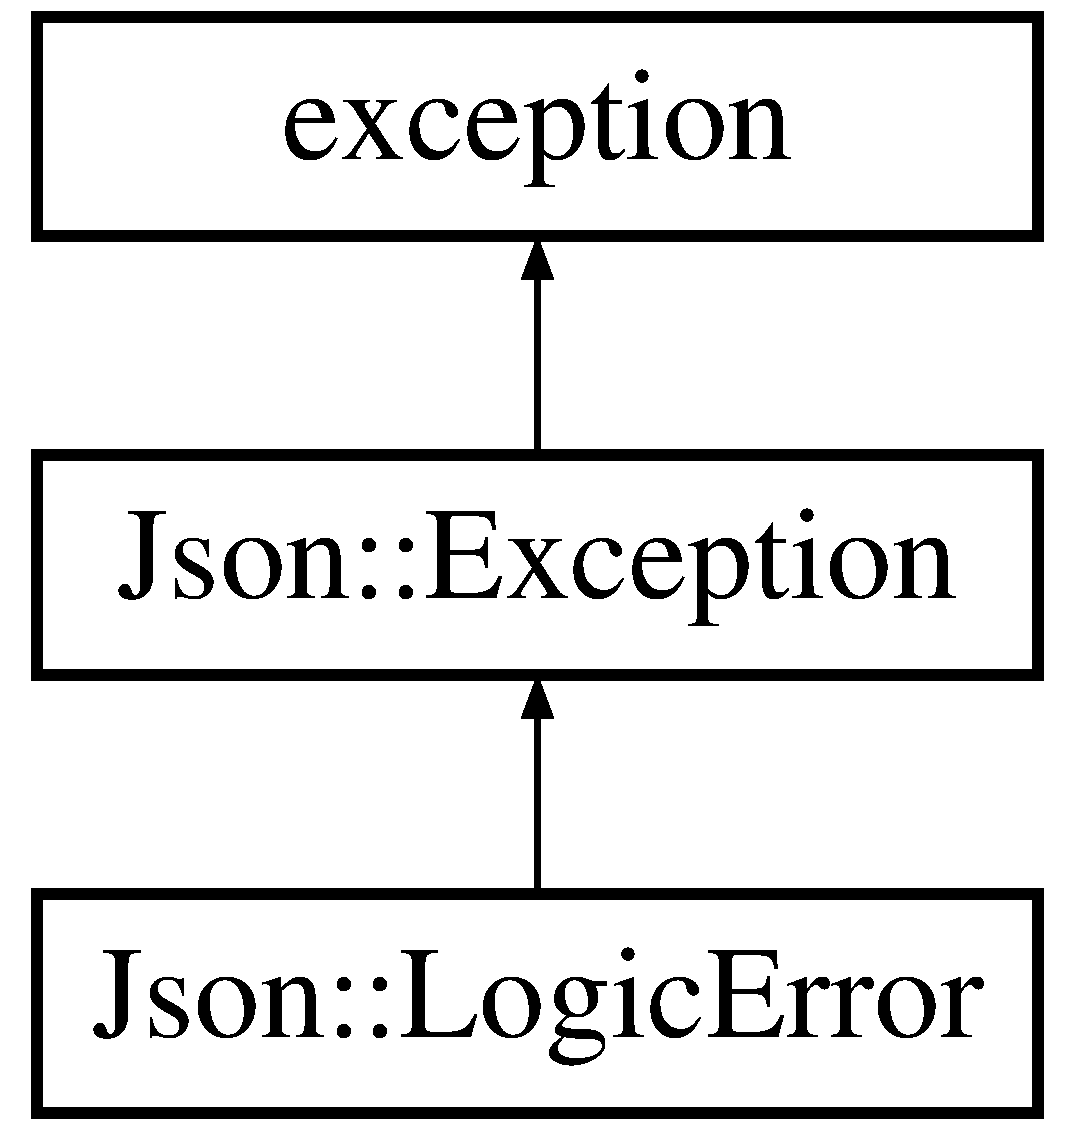
\includegraphics[height=3.000000cm]{classJson_1_1LogicError}
\end{center}
\end{figure}
\subsection*{Public Member Functions}
\begin{DoxyCompactItemize}
\item 
\mbox{\Hypertarget{classJson_1_1LogicError_acca679aa49768a4a1de7b705c67c2919}\label{classJson_1_1LogicError_acca679aa49768a4a1de7b705c67c2919}} 
{\bfseries Logic\+Error} (J\+S\+O\+N\+C\+P\+P\+\_\+\+S\+T\+R\+I\+NG const \&msg)
\end{DoxyCompactItemize}
\subsection*{Additional Inherited Members}


\subsection{Detailed Description}
Exceptions thrown by J\+S\+O\+N\+\_\+\+A\+S\+S\+E\+R\+T/\+J\+S\+O\+N\+\_\+\+F\+A\+IL macros.

These are precondition-\/violations (user bugs) and internal errors (our bugs).

\begin{DoxyRemark}{Remarks}
derived from \hyperlink{classJson_1_1Exception}{Json\+::\+Exception} 
\end{DoxyRemark}


The documentation for this class was generated from the following files\+:\begin{DoxyCompactItemize}
\item 
json/json.\+h\item 
jsoncpp.\+cpp\end{DoxyCompactItemize}

\hypertarget{classTBT_1_1Manager}{}\section{T\+BT\+:\+:Manager Class Reference}
\label{classTBT_1_1Manager}\index{T\+B\+T\+::\+Manager@{T\+B\+T\+::\+Manager}}
\subsection*{Public Member Functions}
\begin{DoxyCompactItemize}
\item 
\mbox{\Hypertarget{classTBT_1_1Manager_a04d5ae5069f1f17ee682f4ae68141687}\label{classTBT_1_1Manager_a04d5ae5069f1f17ee682f4ae68141687}} 
\hyperlink{classTBT_1_1Decoder}{Decoder} $\ast$ {\bfseries find\+Decoder} (uint16\+\_\+t dcc\+Address)
\item 
\mbox{\Hypertarget{classTBT_1_1Manager_a7b20f8a47d78cfd39649722a9fba2f7c}\label{classTBT_1_1Manager_a7b20f8a47d78cfd39649722a9fba2f7c}} 
void {\bfseries register\+Decoder} (\hyperlink{classTBT_1_1Decoder}{Decoder} $\ast$p\+Decoder)
\item 
\mbox{\Hypertarget{classTBT_1_1Manager_a507ac74f4adfbb6173728bebe71e40e6}\label{classTBT_1_1Manager_a507ac74f4adfbb6173728bebe71e40e6}} 
void {\bfseries unregister\+Decoder} (\hyperlink{classTBT_1_1Decoder}{Decoder} $\ast$p\+Decoder)
\item 
\mbox{\Hypertarget{classTBT_1_1Manager_aaac6dc1a57d9c578a3da2243584a8a22}\label{classTBT_1_1Manager_aaac6dc1a57d9c578a3da2243584a8a22}} 
void {\bfseries broadcast\+Loc\+Info\+Changed} (\hyperlink{classTBT_1_1LocDecoder}{Loc\+Decoder} $\ast$p\+Loc)
\item 
\mbox{\Hypertarget{classTBT_1_1Manager_a6e7616a839a1b48d89355bc740ed7793}\label{classTBT_1_1Manager_a6e7616a839a1b48d89355bc740ed7793}} 
void {\bfseries set\+Power\+State} (Power\+State new\+State)
\item 
\mbox{\Hypertarget{classTBT_1_1Manager_a5f5fdba7ccae731f3f348b572fd0ed16}\label{classTBT_1_1Manager_a5f5fdba7ccae731f3f348b572fd0ed16}} 
void {\bfseries set\+Emergency\+Stop} ()
\item 
\mbox{\Hypertarget{classTBT_1_1Manager_a007018b4e6441c9af63cb72f1ffc8a19}\label{classTBT_1_1Manager_a007018b4e6441c9af63cb72f1ffc8a19}} 
void {\bfseries get\+System\+State} (\hyperlink{structTBT_1_1SystemState}{System\+State} $\ast$p\+Msg)
\item 
\mbox{\Hypertarget{classTBT_1_1Manager_a78e5bea49f6662b5f44c1c0aafe4cb75}\label{classTBT_1_1Manager_a78e5bea49f6662b5f44c1c0aafe4cb75}} 
const uint8\+\_\+t \& {\bfseries get\+Central\+State} (void)
\end{DoxyCompactItemize}


The documentation for this class was generated from the following files\+:\begin{DoxyCompactItemize}
\item 
Manager.\+h\item 
Manager.\+cpp\end{DoxyCompactItemize}

\hypertarget{structmbuf}{}\section{mbuf Struct Reference}
\label{structmbuf}\index{mbuf@{mbuf}}
\subsection*{Public Attributes}
\begin{DoxyCompactItemize}
\item 
\mbox{\Hypertarget{structmbuf_ae2a6e23a4997e9aea0908628db2b23d0}\label{structmbuf_ae2a6e23a4997e9aea0908628db2b23d0}} 
char $\ast$ {\bfseries buf}
\item 
\mbox{\Hypertarget{structmbuf_a4da00860609dd46fe8b679d5e1deeac3}\label{structmbuf_a4da00860609dd46fe8b679d5e1deeac3}} 
size\+\_\+t {\bfseries len}
\item 
\mbox{\Hypertarget{structmbuf_ae245d03a50c2891c1fb228093d842270}\label{structmbuf_ae245d03a50c2891c1fb228093d842270}} 
size\+\_\+t {\bfseries size}
\end{DoxyCompactItemize}


The documentation for this struct was generated from the following file\+:\begin{DoxyCompactItemize}
\item 
mongoose.\+h\end{DoxyCompactItemize}

\hypertarget{structmg__add__sock__opts}{}\section{mg\+\_\+add\+\_\+sock\+\_\+opts Struct Reference}
\label{structmg__add__sock__opts}\index{mg\+\_\+add\+\_\+sock\+\_\+opts@{mg\+\_\+add\+\_\+sock\+\_\+opts}}
\subsection*{Public Attributes}
\begin{DoxyCompactItemize}
\item 
\mbox{\Hypertarget{structmg__add__sock__opts_af927a96c42e76f43592b510eca4e1f8e}\label{structmg__add__sock__opts_af927a96c42e76f43592b510eca4e1f8e}} 
void $\ast$ {\bfseries user\+\_\+data}
\item 
\mbox{\Hypertarget{structmg__add__sock__opts_ac836b917617be7c0a38e6a322cdf9cff}\label{structmg__add__sock__opts_ac836b917617be7c0a38e6a322cdf9cff}} 
unsigned int {\bfseries flags}
\item 
\mbox{\Hypertarget{structmg__add__sock__opts_a13c0a3d7dc05ad3873a03a7236735a50}\label{structmg__add__sock__opts_a13c0a3d7dc05ad3873a03a7236735a50}} 
const char $\ast$$\ast$ {\bfseries error\+\_\+string}
\item 
\mbox{\Hypertarget{structmg__add__sock__opts_a3d5516f6481c9a317b4708ec370a9b43}\label{structmg__add__sock__opts_a3d5516f6481c9a317b4708ec370a9b43}} 
struct \hyperlink{structmg__iface}{mg\+\_\+iface} $\ast$ {\bfseries iface}
\end{DoxyCompactItemize}


The documentation for this struct was generated from the following file\+:\begin{DoxyCompactItemize}
\item 
mongoose.\+h\end{DoxyCompactItemize}

\hypertarget{structmg__bind__opts}{}\section{mg\+\_\+bind\+\_\+opts Struct Reference}
\label{structmg__bind__opts}\index{mg\+\_\+bind\+\_\+opts@{mg\+\_\+bind\+\_\+opts}}


{\ttfamily \#include $<$mongoose.\+h$>$}

\subsection*{Public Attributes}
\begin{DoxyCompactItemize}
\item 
void $\ast$ \hyperlink{structmg__bind__opts_a3bd493ef5bd6c8da605b1480a6c189c4_a3bd493ef5bd6c8da605b1480a6c189c4}{user\+\_\+data}
\item 
unsigned int \hyperlink{structmg__bind__opts_ae257fe726a23692a36fb8c92885d4873_ae257fe726a23692a36fb8c92885d4873}{flags}
\item 
const char $\ast$$\ast$ \hyperlink{structmg__bind__opts_a9320251e7b1a273fedc123a3739fb9fa_a9320251e7b1a273fedc123a3739fb9fa}{error\+\_\+string}
\item 
struct \hyperlink{structmg__iface}{mg\+\_\+iface} $\ast$ \hyperlink{structmg__bind__opts_a328924ea266e19c9add95902d82271ad_a328924ea266e19c9add95902d82271ad}{iface}
\end{DoxyCompactItemize}


\subsection{Member Data Documentation}
\mbox{\Hypertarget{structmg__bind__opts_a9320251e7b1a273fedc123a3739fb9fa_a9320251e7b1a273fedc123a3739fb9fa}\label{structmg__bind__opts_a9320251e7b1a273fedc123a3739fb9fa_a9320251e7b1a273fedc123a3739fb9fa}} 
\index{mg\+\_\+bind\+\_\+opts@{mg\+\_\+bind\+\_\+opts}!error\+\_\+string@{error\+\_\+string}}
\index{error\+\_\+string@{error\+\_\+string}!mg\+\_\+bind\+\_\+opts@{mg\+\_\+bind\+\_\+opts}}
\subsubsection{\texorpdfstring{error\+\_\+string}{error\_string}}
{\footnotesize\ttfamily const char$\ast$$\ast$ mg\+\_\+bind\+\_\+opts\+::error\+\_\+string}



Referenced by mg\+\_\+bind\+\_\+opt().

\mbox{\Hypertarget{structmg__bind__opts_ae257fe726a23692a36fb8c92885d4873_ae257fe726a23692a36fb8c92885d4873}\label{structmg__bind__opts_ae257fe726a23692a36fb8c92885d4873_ae257fe726a23692a36fb8c92885d4873}} 
\index{mg\+\_\+bind\+\_\+opts@{mg\+\_\+bind\+\_\+opts}!flags@{flags}}
\index{flags@{flags}!mg\+\_\+bind\+\_\+opts@{mg\+\_\+bind\+\_\+opts}}
\subsubsection{\texorpdfstring{flags}{flags}}
{\footnotesize\ttfamily unsigned int mg\+\_\+bind\+\_\+opts\+::flags}

\mbox{\Hypertarget{structmg__bind__opts_a328924ea266e19c9add95902d82271ad_a328924ea266e19c9add95902d82271ad}\label{structmg__bind__opts_a328924ea266e19c9add95902d82271ad_a328924ea266e19c9add95902d82271ad}} 
\index{mg\+\_\+bind\+\_\+opts@{mg\+\_\+bind\+\_\+opts}!iface@{iface}}
\index{iface@{iface}!mg\+\_\+bind\+\_\+opts@{mg\+\_\+bind\+\_\+opts}}
\subsubsection{\texorpdfstring{iface}{iface}}
{\footnotesize\ttfamily struct \hyperlink{structmg__iface}{mg\+\_\+iface}$\ast$ mg\+\_\+bind\+\_\+opts\+::iface}



Referenced by mg\+\_\+tun\+\_\+do\+\_\+bind().

\mbox{\Hypertarget{structmg__bind__opts_a3bd493ef5bd6c8da605b1480a6c189c4_a3bd493ef5bd6c8da605b1480a6c189c4}\label{structmg__bind__opts_a3bd493ef5bd6c8da605b1480a6c189c4_a3bd493ef5bd6c8da605b1480a6c189c4}} 
\index{mg\+\_\+bind\+\_\+opts@{mg\+\_\+bind\+\_\+opts}!user\+\_\+data@{user\+\_\+data}}
\index{user\+\_\+data@{user\+\_\+data}!mg\+\_\+bind\+\_\+opts@{mg\+\_\+bind\+\_\+opts}}
\subsubsection{\texorpdfstring{user\+\_\+data}{user\_data}}
{\footnotesize\ttfamily void$\ast$ mg\+\_\+bind\+\_\+opts\+::user\+\_\+data}



Referenced by mg\+\_\+bind\+\_\+opt().



The documentation for this struct was generated from the following file\+:\begin{DoxyCompactItemize}
\item 
\hyperlink{mongoose_8h}{mongoose.\+h}\end{DoxyCompactItemize}

\hypertarget{structmg__connect__opts}{}\section{mg\+\_\+connect\+\_\+opts Struct Reference}
\label{structmg__connect__opts}\index{mg\+\_\+connect\+\_\+opts@{mg\+\_\+connect\+\_\+opts}}


{\ttfamily \#include $<$mongoose.\+h$>$}

\subsection*{Public Attributes}
\begin{DoxyCompactItemize}
\item 
void $\ast$ \hyperlink{structmg__connect__opts_a88039c409267c457638a0ebce97d7c5c_a88039c409267c457638a0ebce97d7c5c}{user\+\_\+data}
\item 
unsigned int \hyperlink{structmg__connect__opts_a794f93a8213aa29cdb59fb42075c0ab0_a794f93a8213aa29cdb59fb42075c0ab0}{flags}
\item 
const char $\ast$$\ast$ \hyperlink{structmg__connect__opts_a24fa9723e785487ed74b779c1e30ce75_a24fa9723e785487ed74b779c1e30ce75}{error\+\_\+string}
\item 
struct \hyperlink{structmg__iface}{mg\+\_\+iface} $\ast$ \hyperlink{structmg__connect__opts_a47c10391acd986fe2ff3f4f308bd1637_a47c10391acd986fe2ff3f4f308bd1637}{iface}
\item 
const char $\ast$ \hyperlink{structmg__connect__opts_a53edbf692c49f5ee86d2fe27ebba816c_a53edbf692c49f5ee86d2fe27ebba816c}{nameserver}
\end{DoxyCompactItemize}


\subsection{Member Data Documentation}
\mbox{\Hypertarget{structmg__connect__opts_a24fa9723e785487ed74b779c1e30ce75_a24fa9723e785487ed74b779c1e30ce75}\label{structmg__connect__opts_a24fa9723e785487ed74b779c1e30ce75_a24fa9723e785487ed74b779c1e30ce75}} 
\index{mg\+\_\+connect\+\_\+opts@{mg\+\_\+connect\+\_\+opts}!error\+\_\+string@{error\+\_\+string}}
\index{error\+\_\+string@{error\+\_\+string}!mg\+\_\+connect\+\_\+opts@{mg\+\_\+connect\+\_\+opts}}
\subsubsection{\texorpdfstring{error\+\_\+string}{error\_string}}
{\footnotesize\ttfamily const char$\ast$$\ast$ mg\+\_\+connect\+\_\+opts\+::error\+\_\+string}



Referenced by mg\+\_\+connect\+\_\+http\+\_\+base(), mg\+\_\+connect\+\_\+opt(), and mg\+\_\+parse\+\_\+http\+\_\+basic\+\_\+auth().

\mbox{\Hypertarget{structmg__connect__opts_a794f93a8213aa29cdb59fb42075c0ab0_a794f93a8213aa29cdb59fb42075c0ab0}\label{structmg__connect__opts_a794f93a8213aa29cdb59fb42075c0ab0_a794f93a8213aa29cdb59fb42075c0ab0}} 
\index{mg\+\_\+connect\+\_\+opts@{mg\+\_\+connect\+\_\+opts}!flags@{flags}}
\index{flags@{flags}!mg\+\_\+connect\+\_\+opts@{mg\+\_\+connect\+\_\+opts}}
\subsubsection{\texorpdfstring{flags}{flags}}
{\footnotesize\ttfamily unsigned int mg\+\_\+connect\+\_\+opts\+::flags}



Referenced by mg\+\_\+connect\+\_\+opt().

\mbox{\Hypertarget{structmg__connect__opts_a47c10391acd986fe2ff3f4f308bd1637_a47c10391acd986fe2ff3f4f308bd1637}\label{structmg__connect__opts_a47c10391acd986fe2ff3f4f308bd1637_a47c10391acd986fe2ff3f4f308bd1637}} 
\index{mg\+\_\+connect\+\_\+opts@{mg\+\_\+connect\+\_\+opts}!iface@{iface}}
\index{iface@{iface}!mg\+\_\+connect\+\_\+opts@{mg\+\_\+connect\+\_\+opts}}
\subsubsection{\texorpdfstring{iface}{iface}}
{\footnotesize\ttfamily struct \hyperlink{structmg__iface}{mg\+\_\+iface}$\ast$ mg\+\_\+connect\+\_\+opts\+::iface}

\mbox{\Hypertarget{structmg__connect__opts_a53edbf692c49f5ee86d2fe27ebba816c_a53edbf692c49f5ee86d2fe27ebba816c}\label{structmg__connect__opts_a53edbf692c49f5ee86d2fe27ebba816c_a53edbf692c49f5ee86d2fe27ebba816c}} 
\index{mg\+\_\+connect\+\_\+opts@{mg\+\_\+connect\+\_\+opts}!nameserver@{nameserver}}
\index{nameserver@{nameserver}!mg\+\_\+connect\+\_\+opts@{mg\+\_\+connect\+\_\+opts}}
\subsubsection{\texorpdfstring{nameserver}{nameserver}}
{\footnotesize\ttfamily const char$\ast$ mg\+\_\+connect\+\_\+opts\+::nameserver}



Referenced by mg\+\_\+connect\+\_\+opt().

\mbox{\Hypertarget{structmg__connect__opts_a88039c409267c457638a0ebce97d7c5c_a88039c409267c457638a0ebce97d7c5c}\label{structmg__connect__opts_a88039c409267c457638a0ebce97d7c5c_a88039c409267c457638a0ebce97d7c5c}} 
\index{mg\+\_\+connect\+\_\+opts@{mg\+\_\+connect\+\_\+opts}!user\+\_\+data@{user\+\_\+data}}
\index{user\+\_\+data@{user\+\_\+data}!mg\+\_\+connect\+\_\+opts@{mg\+\_\+connect\+\_\+opts}}
\subsubsection{\texorpdfstring{user\+\_\+data}{user\_data}}
{\footnotesize\ttfamily void$\ast$ mg\+\_\+connect\+\_\+opts\+::user\+\_\+data}



Referenced by mg\+\_\+connect\+\_\+opt().



The documentation for this struct was generated from the following file\+:\begin{DoxyCompactItemize}
\item 
\hyperlink{mongoose_8h}{mongoose.\+h}\end{DoxyCompactItemize}

\hypertarget{structmg__connection}{}\section{mg\+\_\+connection Struct Reference}
\label{structmg__connection}\index{mg\+\_\+connection@{mg\+\_\+connection}}
\subsection*{Public Attributes}
\begin{DoxyCompactItemize}
\item 
\mbox{\Hypertarget{structmg__connection_afcfd89f119a87cba6f6dfec2d2eda5d9}\label{structmg__connection_afcfd89f119a87cba6f6dfec2d2eda5d9}} 
struct \hyperlink{structmg__connection}{mg\+\_\+connection} $\ast$ {\bfseries next}
\item 
\mbox{\Hypertarget{structmg__connection_aa93fd5ca83f11230bc971a68a7fa8d5e}\label{structmg__connection_aa93fd5ca83f11230bc971a68a7fa8d5e}} 
struct \hyperlink{structmg__connection}{mg\+\_\+connection} $\ast$ {\bfseries prev}
\item 
\mbox{\Hypertarget{structmg__connection_a9392bec67d0dc8df58e6c171214ddf8d}\label{structmg__connection_a9392bec67d0dc8df58e6c171214ddf8d}} 
struct \hyperlink{structmg__connection}{mg\+\_\+connection} $\ast$ {\bfseries listener}
\item 
\mbox{\Hypertarget{structmg__connection_ac341f1f2bd18e030fe90a914e4517506}\label{structmg__connection_ac341f1f2bd18e030fe90a914e4517506}} 
struct \hyperlink{structmg__mgr}{mg\+\_\+mgr} $\ast$ {\bfseries mgr}
\item 
\mbox{\Hypertarget{structmg__connection_a608f2461b3dd53e503d6ed3c84ec55b0}\label{structmg__connection_a608f2461b3dd53e503d6ed3c84ec55b0}} 
sock\+\_\+t {\bfseries sock}
\item 
\mbox{\Hypertarget{structmg__connection_aa13a0bd4a2ce3d6384866acb7e00344a}\label{structmg__connection_aa13a0bd4a2ce3d6384866acb7e00344a}} 
int {\bfseries err}
\item 
\mbox{\Hypertarget{structmg__connection_a3dfa1816f5a4b0725d9d04be75bbb3f8}\label{structmg__connection_a3dfa1816f5a4b0725d9d04be75bbb3f8}} 
union \hyperlink{unionsocket__address}{socket\+\_\+address} {\bfseries sa}
\item 
\mbox{\Hypertarget{structmg__connection_ab15e90e7fb7b8719cc7dcc67f45856e1}\label{structmg__connection_ab15e90e7fb7b8719cc7dcc67f45856e1}} 
size\+\_\+t {\bfseries recv\+\_\+mbuf\+\_\+limit}
\item 
\mbox{\Hypertarget{structmg__connection_a72adb9aba4bbe59a9bd591de496713b3}\label{structmg__connection_a72adb9aba4bbe59a9bd591de496713b3}} 
struct \hyperlink{structmbuf}{mbuf} {\bfseries recv\+\_\+mbuf}
\item 
\mbox{\Hypertarget{structmg__connection_a70076f5da9c9d01e77acb3547941671c}\label{structmg__connection_a70076f5da9c9d01e77acb3547941671c}} 
struct \hyperlink{structmbuf}{mbuf} {\bfseries send\+\_\+mbuf}
\item 
\mbox{\Hypertarget{structmg__connection_aaf0f39b26deef84e6c204a176ea1e50a}\label{structmg__connection_aaf0f39b26deef84e6c204a176ea1e50a}} 
time\+\_\+t {\bfseries last\+\_\+io\+\_\+time}
\item 
\mbox{\Hypertarget{structmg__connection_a84d1a7e42f1326c70f61f71e65082dc0}\label{structmg__connection_a84d1a7e42f1326c70f61f71e65082dc0}} 
double {\bfseries ev\+\_\+timer\+\_\+time}
\item 
\mbox{\Hypertarget{structmg__connection_ae6b1f0d002253c0f80371fc5a7bbfc70}\label{structmg__connection_ae6b1f0d002253c0f80371fc5a7bbfc70}} 
mg\+\_\+event\+\_\+handler\+\_\+t {\bfseries proto\+\_\+handler}
\item 
\mbox{\Hypertarget{structmg__connection_a7508851a3c070a1357c226781fa92bb7}\label{structmg__connection_a7508851a3c070a1357c226781fa92bb7}} 
void $\ast$ {\bfseries proto\+\_\+data}
\item 
\mbox{\Hypertarget{structmg__connection_a834e7757b28379b2ca0b8b6c51d7ba95}\label{structmg__connection_a834e7757b28379b2ca0b8b6c51d7ba95}} 
void($\ast$ {\bfseries proto\+\_\+data\+\_\+destructor} )(void $\ast$proto\+\_\+data)
\item 
\mbox{\Hypertarget{structmg__connection_a1f14bd154357c301cce137c9ac1d1edb}\label{structmg__connection_a1f14bd154357c301cce137c9ac1d1edb}} 
mg\+\_\+event\+\_\+handler\+\_\+t {\bfseries handler}
\item 
\mbox{\Hypertarget{structmg__connection_ab6d66a4eacc5d4d15f817ce98f26322d}\label{structmg__connection_ab6d66a4eacc5d4d15f817ce98f26322d}} 
void $\ast$ {\bfseries user\+\_\+data}
\item 
\mbox{\Hypertarget{structmg__connection_ad4386d39d9feedc547a1b1fcc8c5c7de}\label{structmg__connection_ad4386d39d9feedc547a1b1fcc8c5c7de}} 
\begin{tabbing}
xx\=xx\=xx\=xx\=xx\=xx\=xx\=xx\=xx\=\kill
union \{\\
\>void $\ast$ {\bfseries v}\\
\>mg\_event\_handler\_t {\bfseries f}\\
\} {\bfseries priv\_1}\\

\end{tabbing}\item 
\mbox{\Hypertarget{structmg__connection_aeb5efea496ac74ed2e0b8864f4fd6f65}\label{structmg__connection_aeb5efea496ac74ed2e0b8864f4fd6f65}} 
void $\ast$ {\bfseries priv\+\_\+2}
\item 
\mbox{\Hypertarget{structmg__connection_a19cb5ee4c2402582dcf4cb6a4f899136}\label{structmg__connection_a19cb5ee4c2402582dcf4cb6a4f899136}} 
void $\ast$ {\bfseries mgr\+\_\+data}
\item 
\mbox{\Hypertarget{structmg__connection_a6f337461553de516901473bd8bb11a0a}\label{structmg__connection_a6f337461553de516901473bd8bb11a0a}} 
struct \hyperlink{structmg__iface}{mg\+\_\+iface} $\ast$ {\bfseries iface}
\item 
\mbox{\Hypertarget{structmg__connection_aa47edda11152dd7769a76d806a87e1aa}\label{structmg__connection_aa47edda11152dd7769a76d806a87e1aa}} 
unsigned long {\bfseries flags}
\end{DoxyCompactItemize}


The documentation for this struct was generated from the following file\+:\begin{DoxyCompactItemize}
\item 
mongoose.\+h\end{DoxyCompactItemize}

\hypertarget{structmg__dns__header}{}\section{mg\+\_\+dns\+\_\+header Struct Reference}
\label{structmg__dns__header}\index{mg\+\_\+dns\+\_\+header@{mg\+\_\+dns\+\_\+header}}
\subsection*{Public Attributes}
\begin{DoxyCompactItemize}
\item 
uint16\+\_\+t \hyperlink{structmg__dns__header_a00963ebb1d83de6f48f7733679c4b8a7_a00963ebb1d83de6f48f7733679c4b8a7}{transaction\+\_\+id}
\item 
uint16\+\_\+t \hyperlink{structmg__dns__header_a42a3a0530dcceaa67b96f054c1c44aa6_a42a3a0530dcceaa67b96f054c1c44aa6}{flags}
\item 
uint16\+\_\+t \hyperlink{structmg__dns__header_a156d3f5926d1fdb24bcbcba1f273c59a_a156d3f5926d1fdb24bcbcba1f273c59a}{num\+\_\+questions}
\item 
uint16\+\_\+t \hyperlink{structmg__dns__header_a2d577357775702ca340492ca51379b21_a2d577357775702ca340492ca51379b21}{num\+\_\+answers}
\item 
uint16\+\_\+t \hyperlink{structmg__dns__header_a90a7621286acf1c8b78d3ee450dce9b6_a90a7621286acf1c8b78d3ee450dce9b6}{num\+\_\+authority\+\_\+prs}
\item 
uint16\+\_\+t \hyperlink{structmg__dns__header_aed8714aa60f2cc79dc0c81378c2ddb50_aed8714aa60f2cc79dc0c81378c2ddb50}{num\+\_\+other\+\_\+prs}
\end{DoxyCompactItemize}


\subsection{Member Data Documentation}
\mbox{\Hypertarget{structmg__dns__header_a42a3a0530dcceaa67b96f054c1c44aa6_a42a3a0530dcceaa67b96f054c1c44aa6}\label{structmg__dns__header_a42a3a0530dcceaa67b96f054c1c44aa6_a42a3a0530dcceaa67b96f054c1c44aa6}} 
\index{mg\+\_\+dns\+\_\+header@{mg\+\_\+dns\+\_\+header}!flags@{flags}}
\index{flags@{flags}!mg\+\_\+dns\+\_\+header@{mg\+\_\+dns\+\_\+header}}
\subsubsection{\texorpdfstring{flags}{flags}}
{\footnotesize\ttfamily uint16\+\_\+t mg\+\_\+dns\+\_\+header\+::flags}



Referenced by mg\+\_\+dns\+\_\+insert\+\_\+header(), and mg\+\_\+parse\+\_\+dns().

\mbox{\Hypertarget{structmg__dns__header_a2d577357775702ca340492ca51379b21_a2d577357775702ca340492ca51379b21}\label{structmg__dns__header_a2d577357775702ca340492ca51379b21_a2d577357775702ca340492ca51379b21}} 
\index{mg\+\_\+dns\+\_\+header@{mg\+\_\+dns\+\_\+header}!num\+\_\+answers@{num\+\_\+answers}}
\index{num\+\_\+answers@{num\+\_\+answers}!mg\+\_\+dns\+\_\+header@{mg\+\_\+dns\+\_\+header}}
\subsubsection{\texorpdfstring{num\+\_\+answers}{num\_answers}}
{\footnotesize\ttfamily uint16\+\_\+t mg\+\_\+dns\+\_\+header\+::num\+\_\+answers}



Referenced by mg\+\_\+dns\+\_\+insert\+\_\+header(), and mg\+\_\+parse\+\_\+dns().

\mbox{\Hypertarget{structmg__dns__header_a90a7621286acf1c8b78d3ee450dce9b6_a90a7621286acf1c8b78d3ee450dce9b6}\label{structmg__dns__header_a90a7621286acf1c8b78d3ee450dce9b6_a90a7621286acf1c8b78d3ee450dce9b6}} 
\index{mg\+\_\+dns\+\_\+header@{mg\+\_\+dns\+\_\+header}!num\+\_\+authority\+\_\+prs@{num\+\_\+authority\+\_\+prs}}
\index{num\+\_\+authority\+\_\+prs@{num\+\_\+authority\+\_\+prs}!mg\+\_\+dns\+\_\+header@{mg\+\_\+dns\+\_\+header}}
\subsubsection{\texorpdfstring{num\+\_\+authority\+\_\+prs}{num\_authority\_prs}}
{\footnotesize\ttfamily uint16\+\_\+t mg\+\_\+dns\+\_\+header\+::num\+\_\+authority\+\_\+prs}

\mbox{\Hypertarget{structmg__dns__header_aed8714aa60f2cc79dc0c81378c2ddb50_aed8714aa60f2cc79dc0c81378c2ddb50}\label{structmg__dns__header_aed8714aa60f2cc79dc0c81378c2ddb50_aed8714aa60f2cc79dc0c81378c2ddb50}} 
\index{mg\+\_\+dns\+\_\+header@{mg\+\_\+dns\+\_\+header}!num\+\_\+other\+\_\+prs@{num\+\_\+other\+\_\+prs}}
\index{num\+\_\+other\+\_\+prs@{num\+\_\+other\+\_\+prs}!mg\+\_\+dns\+\_\+header@{mg\+\_\+dns\+\_\+header}}
\subsubsection{\texorpdfstring{num\+\_\+other\+\_\+prs}{num\_other\_prs}}
{\footnotesize\ttfamily uint16\+\_\+t mg\+\_\+dns\+\_\+header\+::num\+\_\+other\+\_\+prs}

\mbox{\Hypertarget{structmg__dns__header_a156d3f5926d1fdb24bcbcba1f273c59a_a156d3f5926d1fdb24bcbcba1f273c59a}\label{structmg__dns__header_a156d3f5926d1fdb24bcbcba1f273c59a_a156d3f5926d1fdb24bcbcba1f273c59a}} 
\index{mg\+\_\+dns\+\_\+header@{mg\+\_\+dns\+\_\+header}!num\+\_\+questions@{num\+\_\+questions}}
\index{num\+\_\+questions@{num\+\_\+questions}!mg\+\_\+dns\+\_\+header@{mg\+\_\+dns\+\_\+header}}
\subsubsection{\texorpdfstring{num\+\_\+questions}{num\_questions}}
{\footnotesize\ttfamily uint16\+\_\+t mg\+\_\+dns\+\_\+header\+::num\+\_\+questions}



Referenced by mg\+\_\+dns\+\_\+insert\+\_\+header(), and mg\+\_\+parse\+\_\+dns().

\mbox{\Hypertarget{structmg__dns__header_a00963ebb1d83de6f48f7733679c4b8a7_a00963ebb1d83de6f48f7733679c4b8a7}\label{structmg__dns__header_a00963ebb1d83de6f48f7733679c4b8a7_a00963ebb1d83de6f48f7733679c4b8a7}} 
\index{mg\+\_\+dns\+\_\+header@{mg\+\_\+dns\+\_\+header}!transaction\+\_\+id@{transaction\+\_\+id}}
\index{transaction\+\_\+id@{transaction\+\_\+id}!mg\+\_\+dns\+\_\+header@{mg\+\_\+dns\+\_\+header}}
\subsubsection{\texorpdfstring{transaction\+\_\+id}{transaction\_id}}
{\footnotesize\ttfamily uint16\+\_\+t mg\+\_\+dns\+\_\+header\+::transaction\+\_\+id}



Referenced by mg\+\_\+dns\+\_\+insert\+\_\+header(), and mg\+\_\+parse\+\_\+dns().



The documentation for this struct was generated from the following file\+:\begin{DoxyCompactItemize}
\item 
\hyperlink{mongoose_8c}{mongoose.\+c}\end{DoxyCompactItemize}

\hypertarget{structmg__dns__message}{}\section{mg\+\_\+dns\+\_\+message Struct Reference}
\label{structmg__dns__message}\index{mg\+\_\+dns\+\_\+message@{mg\+\_\+dns\+\_\+message}}


{\ttfamily \#include $<$mongoose.\+h$>$}

\subsection*{Public Attributes}
\begin{DoxyCompactItemize}
\item 
struct \hyperlink{structmg__str}{mg\+\_\+str} \hyperlink{structmg__dns__message_ae8543b2a3044c785b4bf0dc4fc39beff_ae8543b2a3044c785b4bf0dc4fc39beff}{pkt}
\item 
uint16\+\_\+t \hyperlink{structmg__dns__message_a87f916bb55651d46ce74f930a5e08327_a87f916bb55651d46ce74f930a5e08327}{flags}
\item 
uint16\+\_\+t \hyperlink{structmg__dns__message_afb4a01337779347f74a214c7a273ebcb_afb4a01337779347f74a214c7a273ebcb}{transaction\+\_\+id}
\item 
int \hyperlink{structmg__dns__message_a035ced22ef43b6b23ad6df3ad3aad126_a035ced22ef43b6b23ad6df3ad3aad126}{num\+\_\+questions}
\item 
int \hyperlink{structmg__dns__message_a6ebecefbdcb5c292f439123b7c780517_a6ebecefbdcb5c292f439123b7c780517}{num\+\_\+answers}
\item 
struct \hyperlink{structmg__dns__resource__record}{mg\+\_\+dns\+\_\+resource\+\_\+record} \hyperlink{structmg__dns__message_a866a83825f2daa4043aa20acded4f007_a866a83825f2daa4043aa20acded4f007}{questions} \mbox{[}\hyperlink{mongoose_8h_a84f36ff9caf50e0d70d10244a2c64b45_a84f36ff9caf50e0d70d10244a2c64b45}{M\+G\+\_\+\+M\+A\+X\+\_\+\+D\+N\+S\+\_\+\+Q\+U\+E\+S\+T\+I\+O\+NS}\mbox{]}
\item 
struct \hyperlink{structmg__dns__resource__record}{mg\+\_\+dns\+\_\+resource\+\_\+record} \hyperlink{structmg__dns__message_a76e7c9d2d5f7f621df2d2551f0163e01_a76e7c9d2d5f7f621df2d2551f0163e01}{answers} \mbox{[}\hyperlink{mongoose_8h_a1832d47a93efb88b807286ed1ae80646_a1832d47a93efb88b807286ed1ae80646}{M\+G\+\_\+\+M\+A\+X\+\_\+\+D\+N\+S\+\_\+\+A\+N\+S\+W\+E\+RS}\mbox{]}
\end{DoxyCompactItemize}


\subsection{Member Data Documentation}
\mbox{\Hypertarget{structmg__dns__message_a76e7c9d2d5f7f621df2d2551f0163e01_a76e7c9d2d5f7f621df2d2551f0163e01}\label{structmg__dns__message_a76e7c9d2d5f7f621df2d2551f0163e01_a76e7c9d2d5f7f621df2d2551f0163e01}} 
\index{mg\+\_\+dns\+\_\+message@{mg\+\_\+dns\+\_\+message}!answers@{answers}}
\index{answers@{answers}!mg\+\_\+dns\+\_\+message@{mg\+\_\+dns\+\_\+message}}
\subsubsection{\texorpdfstring{answers}{answers}}
{\footnotesize\ttfamily struct \hyperlink{structmg__dns__resource__record}{mg\+\_\+dns\+\_\+resource\+\_\+record} mg\+\_\+dns\+\_\+message\+::answers\mbox{[}\hyperlink{mongoose_8h_a1832d47a93efb88b807286ed1ae80646_a1832d47a93efb88b807286ed1ae80646}{M\+G\+\_\+\+M\+A\+X\+\_\+\+D\+N\+S\+\_\+\+A\+N\+S\+W\+E\+RS}\mbox{]}}



Referenced by mg\+\_\+dns\+\_\+next\+\_\+record(), mg\+\_\+parse\+\_\+dns(), mg\+\_\+set\+\_\+protocol\+\_\+dns(), and resolve\+\_\+cb().

\mbox{\Hypertarget{structmg__dns__message_a87f916bb55651d46ce74f930a5e08327_a87f916bb55651d46ce74f930a5e08327}\label{structmg__dns__message_a87f916bb55651d46ce74f930a5e08327_a87f916bb55651d46ce74f930a5e08327}} 
\index{mg\+\_\+dns\+\_\+message@{mg\+\_\+dns\+\_\+message}!flags@{flags}}
\index{flags@{flags}!mg\+\_\+dns\+\_\+message@{mg\+\_\+dns\+\_\+message}}
\subsubsection{\texorpdfstring{flags}{flags}}
{\footnotesize\ttfamily uint16\+\_\+t mg\+\_\+dns\+\_\+message\+::flags}



Referenced by dns\+\_\+handler(), mg\+\_\+dns\+\_\+insert\+\_\+header(), mg\+\_\+parse\+\_\+dns(), and mg\+\_\+send\+\_\+dns\+\_\+query().

\mbox{\Hypertarget{structmg__dns__message_a6ebecefbdcb5c292f439123b7c780517_a6ebecefbdcb5c292f439123b7c780517}\label{structmg__dns__message_a6ebecefbdcb5c292f439123b7c780517_a6ebecefbdcb5c292f439123b7c780517}} 
\index{mg\+\_\+dns\+\_\+message@{mg\+\_\+dns\+\_\+message}!num\+\_\+answers@{num\+\_\+answers}}
\index{num\+\_\+answers@{num\+\_\+answers}!mg\+\_\+dns\+\_\+message@{mg\+\_\+dns\+\_\+message}}
\subsubsection{\texorpdfstring{num\+\_\+answers}{num\_answers}}
{\footnotesize\ttfamily int mg\+\_\+dns\+\_\+message\+::num\+\_\+answers}



Referenced by mg\+\_\+dns\+\_\+insert\+\_\+header(), mg\+\_\+dns\+\_\+next\+\_\+record(), mg\+\_\+parse\+\_\+dns(), mg\+\_\+resolve\+\_\+async\+\_\+eh(), mg\+\_\+set\+\_\+protocol\+\_\+dns(), and resolve\+\_\+cb().

\mbox{\Hypertarget{structmg__dns__message_a035ced22ef43b6b23ad6df3ad3aad126_a035ced22ef43b6b23ad6df3ad3aad126}\label{structmg__dns__message_a035ced22ef43b6b23ad6df3ad3aad126_a035ced22ef43b6b23ad6df3ad3aad126}} 
\index{mg\+\_\+dns\+\_\+message@{mg\+\_\+dns\+\_\+message}!num\+\_\+questions@{num\+\_\+questions}}
\index{num\+\_\+questions@{num\+\_\+questions}!mg\+\_\+dns\+\_\+message@{mg\+\_\+dns\+\_\+message}}
\subsubsection{\texorpdfstring{num\+\_\+questions}{num\_questions}}
{\footnotesize\ttfamily int mg\+\_\+dns\+\_\+message\+::num\+\_\+questions}



Referenced by mg\+\_\+dns\+\_\+copy\+\_\+questions(), mg\+\_\+dns\+\_\+insert\+\_\+header(), mg\+\_\+parse\+\_\+dns(), and mg\+\_\+send\+\_\+dns\+\_\+query().

\mbox{\Hypertarget{structmg__dns__message_ae8543b2a3044c785b4bf0dc4fc39beff_ae8543b2a3044c785b4bf0dc4fc39beff}\label{structmg__dns__message_ae8543b2a3044c785b4bf0dc4fc39beff_ae8543b2a3044c785b4bf0dc4fc39beff}} 
\index{mg\+\_\+dns\+\_\+message@{mg\+\_\+dns\+\_\+message}!pkt@{pkt}}
\index{pkt@{pkt}!mg\+\_\+dns\+\_\+message@{mg\+\_\+dns\+\_\+message}}
\subsubsection{\texorpdfstring{pkt}{pkt}}
{\footnotesize\ttfamily struct \hyperlink{structmg__str}{mg\+\_\+str} mg\+\_\+dns\+\_\+message\+::pkt}



Referenced by mg\+\_\+dns\+\_\+copy\+\_\+questions(), mg\+\_\+dns\+\_\+parse\+\_\+record\+\_\+data(), mg\+\_\+dns\+\_\+uncompress\+\_\+name(), and mg\+\_\+parse\+\_\+dns().

\mbox{\Hypertarget{structmg__dns__message_a866a83825f2daa4043aa20acded4f007_a866a83825f2daa4043aa20acded4f007}\label{structmg__dns__message_a866a83825f2daa4043aa20acded4f007_a866a83825f2daa4043aa20acded4f007}} 
\index{mg\+\_\+dns\+\_\+message@{mg\+\_\+dns\+\_\+message}!questions@{questions}}
\index{questions@{questions}!mg\+\_\+dns\+\_\+message@{mg\+\_\+dns\+\_\+message}}
\subsubsection{\texorpdfstring{questions}{questions}}
{\footnotesize\ttfamily struct \hyperlink{structmg__dns__resource__record}{mg\+\_\+dns\+\_\+resource\+\_\+record} mg\+\_\+dns\+\_\+message\+::questions\mbox{[}\hyperlink{mongoose_8h_a84f36ff9caf50e0d70d10244a2c64b45_a84f36ff9caf50e0d70d10244a2c64b45}{M\+G\+\_\+\+M\+A\+X\+\_\+\+D\+N\+S\+\_\+\+Q\+U\+E\+S\+T\+I\+O\+NS}\mbox{]}}



Referenced by mg\+\_\+dns\+\_\+copy\+\_\+questions(), mg\+\_\+parse\+\_\+dns(), and mg\+\_\+send\+\_\+dns\+\_\+query().

\mbox{\Hypertarget{structmg__dns__message_afb4a01337779347f74a214c7a273ebcb_afb4a01337779347f74a214c7a273ebcb}\label{structmg__dns__message_afb4a01337779347f74a214c7a273ebcb_afb4a01337779347f74a214c7a273ebcb}} 
\index{mg\+\_\+dns\+\_\+message@{mg\+\_\+dns\+\_\+message}!transaction\+\_\+id@{transaction\+\_\+id}}
\index{transaction\+\_\+id@{transaction\+\_\+id}!mg\+\_\+dns\+\_\+message@{mg\+\_\+dns\+\_\+message}}
\subsubsection{\texorpdfstring{transaction\+\_\+id}{transaction\_id}}
{\footnotesize\ttfamily uint16\+\_\+t mg\+\_\+dns\+\_\+message\+::transaction\+\_\+id}



Referenced by mg\+\_\+dns\+\_\+insert\+\_\+header(), mg\+\_\+parse\+\_\+dns(), and mg\+\_\+send\+\_\+dns\+\_\+query().



The documentation for this struct was generated from the following file\+:\begin{DoxyCompactItemize}
\item 
\hyperlink{mongoose_8h}{mongoose.\+h}\end{DoxyCompactItemize}

\hypertarget{structmg__dns__resource__record}{}\section{mg\+\_\+dns\+\_\+resource\+\_\+record Struct Reference}
\label{structmg__dns__resource__record}\index{mg\+\_\+dns\+\_\+resource\+\_\+record@{mg\+\_\+dns\+\_\+resource\+\_\+record}}


{\ttfamily \#include $<$mongoose.\+h$>$}

\subsection*{Public Attributes}
\begin{DoxyCompactItemize}
\item 
struct \hyperlink{structmg__str}{mg\+\_\+str} \hyperlink{structmg__dns__resource__record_afd27e187a02127a98a04757013aecd48_afd27e187a02127a98a04757013aecd48}{name}
\item 
int \hyperlink{structmg__dns__resource__record_a9d314632522fcca513858285c639bee9_a9d314632522fcca513858285c639bee9}{rtype}
\item 
int \hyperlink{structmg__dns__resource__record_a9be7dc2d7ef4e2dc20413289a55f6ff7_a9be7dc2d7ef4e2dc20413289a55f6ff7}{rclass}
\item 
int \hyperlink{structmg__dns__resource__record_aa5d1c1a7ba2d02908c27fab68ded25be_aa5d1c1a7ba2d02908c27fab68ded25be}{ttl}
\item 
enum \hyperlink{mongoose_8h_abc1e540c922be63eea4488f520e3523d_abc1e540c922be63eea4488f520e3523d}{mg\+\_\+dns\+\_\+resource\+\_\+record\+\_\+kind} \hyperlink{structmg__dns__resource__record_a6f9d5dda9d8ae9240a74282c44d4a555_a6f9d5dda9d8ae9240a74282c44d4a555}{kind}
\item 
struct \hyperlink{structmg__str}{mg\+\_\+str} \hyperlink{structmg__dns__resource__record_ac169801d0c9ce94137fcce9a3f629152_ac169801d0c9ce94137fcce9a3f629152}{rdata}
\end{DoxyCompactItemize}


\subsection{Member Data Documentation}
\mbox{\Hypertarget{structmg__dns__resource__record_a6f9d5dda9d8ae9240a74282c44d4a555_a6f9d5dda9d8ae9240a74282c44d4a555}\label{structmg__dns__resource__record_a6f9d5dda9d8ae9240a74282c44d4a555_a6f9d5dda9d8ae9240a74282c44d4a555}} 
\index{mg\+\_\+dns\+\_\+resource\+\_\+record@{mg\+\_\+dns\+\_\+resource\+\_\+record}!kind@{kind}}
\index{kind@{kind}!mg\+\_\+dns\+\_\+resource\+\_\+record@{mg\+\_\+dns\+\_\+resource\+\_\+record}}
\subsubsection{\texorpdfstring{kind}{kind}}
{\footnotesize\ttfamily enum \hyperlink{mongoose_8h_abc1e540c922be63eea4488f520e3523d_abc1e540c922be63eea4488f520e3523d}{mg\+\_\+dns\+\_\+resource\+\_\+record\+\_\+kind} mg\+\_\+dns\+\_\+resource\+\_\+record\+::kind}



Referenced by mg\+\_\+dns\+\_\+encode\+\_\+record(), mg\+\_\+parse\+\_\+dns\+\_\+resource\+\_\+record(), mg\+\_\+send\+\_\+dns\+\_\+query(), and mg\+\_\+set\+\_\+protocol\+\_\+dns().

\mbox{\Hypertarget{structmg__dns__resource__record_afd27e187a02127a98a04757013aecd48_afd27e187a02127a98a04757013aecd48}\label{structmg__dns__resource__record_afd27e187a02127a98a04757013aecd48_afd27e187a02127a98a04757013aecd48}} 
\index{mg\+\_\+dns\+\_\+resource\+\_\+record@{mg\+\_\+dns\+\_\+resource\+\_\+record}!name@{name}}
\index{name@{name}!mg\+\_\+dns\+\_\+resource\+\_\+record@{mg\+\_\+dns\+\_\+resource\+\_\+record}}
\subsubsection{\texorpdfstring{name}{name}}
{\footnotesize\ttfamily struct \hyperlink{structmg__str}{mg\+\_\+str} mg\+\_\+dns\+\_\+resource\+\_\+record\+::name}



Referenced by mg\+\_\+dns\+\_\+copy\+\_\+questions(), mg\+\_\+dns\+\_\+encode\+\_\+name(), mg\+\_\+parse\+\_\+dns\+\_\+resource\+\_\+record(), and mg\+\_\+set\+\_\+protocol\+\_\+dns().

\mbox{\Hypertarget{structmg__dns__resource__record_a9be7dc2d7ef4e2dc20413289a55f6ff7_a9be7dc2d7ef4e2dc20413289a55f6ff7}\label{structmg__dns__resource__record_a9be7dc2d7ef4e2dc20413289a55f6ff7_a9be7dc2d7ef4e2dc20413289a55f6ff7}} 
\index{mg\+\_\+dns\+\_\+resource\+\_\+record@{mg\+\_\+dns\+\_\+resource\+\_\+record}!rclass@{rclass}}
\index{rclass@{rclass}!mg\+\_\+dns\+\_\+resource\+\_\+record@{mg\+\_\+dns\+\_\+resource\+\_\+record}}
\subsubsection{\texorpdfstring{rclass}{rclass}}
{\footnotesize\ttfamily int mg\+\_\+dns\+\_\+resource\+\_\+record\+::rclass}



Referenced by mg\+\_\+dns\+\_\+encode\+\_\+record(), mg\+\_\+parse\+\_\+dns\+\_\+resource\+\_\+record(), and mg\+\_\+send\+\_\+dns\+\_\+query().

\mbox{\Hypertarget{structmg__dns__resource__record_ac169801d0c9ce94137fcce9a3f629152_ac169801d0c9ce94137fcce9a3f629152}\label{structmg__dns__resource__record_ac169801d0c9ce94137fcce9a3f629152_ac169801d0c9ce94137fcce9a3f629152}} 
\index{mg\+\_\+dns\+\_\+resource\+\_\+record@{mg\+\_\+dns\+\_\+resource\+\_\+record}!rdata@{rdata}}
\index{rdata@{rdata}!mg\+\_\+dns\+\_\+resource\+\_\+record@{mg\+\_\+dns\+\_\+resource\+\_\+record}}
\subsubsection{\texorpdfstring{rdata}{rdata}}
{\footnotesize\ttfamily struct \hyperlink{structmg__str}{mg\+\_\+str} mg\+\_\+dns\+\_\+resource\+\_\+record\+::rdata}



Referenced by mg\+\_\+dns\+\_\+parse\+\_\+record\+\_\+data(), and mg\+\_\+parse\+\_\+dns\+\_\+resource\+\_\+record().

\mbox{\Hypertarget{structmg__dns__resource__record_a9d314632522fcca513858285c639bee9_a9d314632522fcca513858285c639bee9}\label{structmg__dns__resource__record_a9d314632522fcca513858285c639bee9_a9d314632522fcca513858285c639bee9}} 
\index{mg\+\_\+dns\+\_\+resource\+\_\+record@{mg\+\_\+dns\+\_\+resource\+\_\+record}!rtype@{rtype}}
\index{rtype@{rtype}!mg\+\_\+dns\+\_\+resource\+\_\+record@{mg\+\_\+dns\+\_\+resource\+\_\+record}}
\subsubsection{\texorpdfstring{rtype}{rtype}}
{\footnotesize\ttfamily int mg\+\_\+dns\+\_\+resource\+\_\+record\+::rtype}



Referenced by mg\+\_\+dns\+\_\+encode\+\_\+record(), mg\+\_\+dns\+\_\+next\+\_\+record(), mg\+\_\+dns\+\_\+parse\+\_\+record\+\_\+data(), mg\+\_\+parse\+\_\+dns\+\_\+resource\+\_\+record(), mg\+\_\+send\+\_\+dns\+\_\+query(), and resolve\+\_\+cb().

\mbox{\Hypertarget{structmg__dns__resource__record_aa5d1c1a7ba2d02908c27fab68ded25be_aa5d1c1a7ba2d02908c27fab68ded25be}\label{structmg__dns__resource__record_aa5d1c1a7ba2d02908c27fab68ded25be_aa5d1c1a7ba2d02908c27fab68ded25be}} 
\index{mg\+\_\+dns\+\_\+resource\+\_\+record@{mg\+\_\+dns\+\_\+resource\+\_\+record}!ttl@{ttl}}
\index{ttl@{ttl}!mg\+\_\+dns\+\_\+resource\+\_\+record@{mg\+\_\+dns\+\_\+resource\+\_\+record}}
\subsubsection{\texorpdfstring{ttl}{ttl}}
{\footnotesize\ttfamily int mg\+\_\+dns\+\_\+resource\+\_\+record\+::ttl}



Referenced by mg\+\_\+dns\+\_\+encode\+\_\+record(), and mg\+\_\+parse\+\_\+dns\+\_\+resource\+\_\+record().



The documentation for this struct was generated from the following file\+:\begin{DoxyCompactItemize}
\item 
\hyperlink{mongoose_8h}{mongoose.\+h}\end{DoxyCompactItemize}

\hypertarget{structmg__http__endpoint}{}\section{mg\+\_\+http\+\_\+endpoint Struct Reference}
\label{structmg__http__endpoint}\index{mg\+\_\+http\+\_\+endpoint@{mg\+\_\+http\+\_\+endpoint}}
\subsection*{Public Attributes}
\begin{DoxyCompactItemize}
\item 
\mbox{\Hypertarget{structmg__http__endpoint_a28fd60f7d7ade3f17130287713340ab7}\label{structmg__http__endpoint_a28fd60f7d7ade3f17130287713340ab7}} 
struct \hyperlink{structmg__http__endpoint}{mg\+\_\+http\+\_\+endpoint} $\ast$ {\bfseries next}
\item 
\mbox{\Hypertarget{structmg__http__endpoint_a72024abf72236a0bd7a529182ce78d36}\label{structmg__http__endpoint_a72024abf72236a0bd7a529182ce78d36}} 
struct \hyperlink{structmg__str}{mg\+\_\+str} {\bfseries uri\+\_\+pattern}
\item 
\mbox{\Hypertarget{structmg__http__endpoint_a19a0e4a59560c9d0b02eaf9d91f50738}\label{structmg__http__endpoint_a19a0e4a59560c9d0b02eaf9d91f50738}} 
char $\ast$ {\bfseries auth\+\_\+domain}
\item 
\mbox{\Hypertarget{structmg__http__endpoint_ac54f73eec84df2b4caeb729e9a8fb56e}\label{structmg__http__endpoint_ac54f73eec84df2b4caeb729e9a8fb56e}} 
char $\ast$ {\bfseries auth\+\_\+file}
\item 
\mbox{\Hypertarget{structmg__http__endpoint_a24176c5ff8bb9ffb89a8f553e8e066e0}\label{structmg__http__endpoint_a24176c5ff8bb9ffb89a8f553e8e066e0}} 
mg\+\_\+event\+\_\+handler\+\_\+t {\bfseries handler}
\end{DoxyCompactItemize}


The documentation for this struct was generated from the following file\+:\begin{DoxyCompactItemize}
\item 
mongoose.\+c\end{DoxyCompactItemize}

\hypertarget{structmg__http__endpoint__opts}{}\section{mg\+\_\+http\+\_\+endpoint\+\_\+opts Struct Reference}
\label{structmg__http__endpoint__opts}\index{mg\+\_\+http\+\_\+endpoint\+\_\+opts@{mg\+\_\+http\+\_\+endpoint\+\_\+opts}}
\subsection*{Public Attributes}
\begin{DoxyCompactItemize}
\item 
\mbox{\Hypertarget{structmg__http__endpoint__opts_acdb6a63492d91f7e1c4f34242ba6be1d}\label{structmg__http__endpoint__opts_acdb6a63492d91f7e1c4f34242ba6be1d}} 
void $\ast$ {\bfseries user\+\_\+data}
\item 
\mbox{\Hypertarget{structmg__http__endpoint__opts_a5af8bb0311abbac3f9388c4b95210dac}\label{structmg__http__endpoint__opts_a5af8bb0311abbac3f9388c4b95210dac}} 
const char $\ast$ {\bfseries auth\+\_\+domain}
\item 
\mbox{\Hypertarget{structmg__http__endpoint__opts_a57ae875a1cc356870d396f3d864d2fc8}\label{structmg__http__endpoint__opts_a57ae875a1cc356870d396f3d864d2fc8}} 
const char $\ast$ {\bfseries auth\+\_\+file}
\end{DoxyCompactItemize}


The documentation for this struct was generated from the following file\+:\begin{DoxyCompactItemize}
\item 
mongoose.\+h\end{DoxyCompactItemize}

\hypertarget{structmg__http__multipart__part}{}\section{mg\+\_\+http\+\_\+multipart\+\_\+part Struct Reference}
\label{structmg__http__multipart__part}\index{mg\+\_\+http\+\_\+multipart\+\_\+part@{mg\+\_\+http\+\_\+multipart\+\_\+part}}


{\ttfamily \#include $<$mongoose.\+h$>$}

\subsection*{Public Attributes}
\begin{DoxyCompactItemize}
\item 
const char $\ast$ \hyperlink{structmg__http__multipart__part_a838efa2eb99ad6cecd6ae714d4775091_a838efa2eb99ad6cecd6ae714d4775091}{file\+\_\+name}
\item 
const char $\ast$ \hyperlink{structmg__http__multipart__part_af3c6e9825e31f000ec9e26c016eaa707_af3c6e9825e31f000ec9e26c016eaa707}{var\+\_\+name}
\item 
struct \hyperlink{structmg__str}{mg\+\_\+str} \hyperlink{structmg__http__multipart__part_a803db4feee24a462665d487acbeb1953_a803db4feee24a462665d487acbeb1953}{data}
\item 
int \hyperlink{structmg__http__multipart__part_a728d1246c153ef43fb1f821bee61925a_a728d1246c153ef43fb1f821bee61925a}{status}
\item 
void $\ast$ \hyperlink{structmg__http__multipart__part_ab0c10748e6a40d9c85b4ec0ac98047bd_ab0c10748e6a40d9c85b4ec0ac98047bd}{user\+\_\+data}
\end{DoxyCompactItemize}


\subsection{Member Data Documentation}
\mbox{\Hypertarget{structmg__http__multipart__part_a803db4feee24a462665d487acbeb1953_a803db4feee24a462665d487acbeb1953}\label{structmg__http__multipart__part_a803db4feee24a462665d487acbeb1953_a803db4feee24a462665d487acbeb1953}} 
\index{mg\+\_\+http\+\_\+multipart\+\_\+part@{mg\+\_\+http\+\_\+multipart\+\_\+part}!data@{data}}
\index{data@{data}!mg\+\_\+http\+\_\+multipart\+\_\+part@{mg\+\_\+http\+\_\+multipart\+\_\+part}}
\subsubsection{\texorpdfstring{data}{data}}
{\footnotesize\ttfamily struct \hyperlink{structmg__str}{mg\+\_\+str} mg\+\_\+http\+\_\+multipart\+\_\+part\+::data}



Referenced by mg\+\_\+get\+\_\+line\+\_\+len(), and mg\+\_\+parse\+\_\+http\+\_\+basic\+\_\+auth().

\mbox{\Hypertarget{structmg__http__multipart__part_a838efa2eb99ad6cecd6ae714d4775091_a838efa2eb99ad6cecd6ae714d4775091}\label{structmg__http__multipart__part_a838efa2eb99ad6cecd6ae714d4775091_a838efa2eb99ad6cecd6ae714d4775091}} 
\index{mg\+\_\+http\+\_\+multipart\+\_\+part@{mg\+\_\+http\+\_\+multipart\+\_\+part}!file\+\_\+name@{file\+\_\+name}}
\index{file\+\_\+name@{file\+\_\+name}!mg\+\_\+http\+\_\+multipart\+\_\+part@{mg\+\_\+http\+\_\+multipart\+\_\+part}}
\subsubsection{\texorpdfstring{file\+\_\+name}{file\_name}}
{\footnotesize\ttfamily const char$\ast$ mg\+\_\+http\+\_\+multipart\+\_\+part\+::file\+\_\+name}



Referenced by mg\+\_\+get\+\_\+line\+\_\+len(), mg\+\_\+http\+\_\+handler(), and mg\+\_\+parse\+\_\+http\+\_\+basic\+\_\+auth().

\mbox{\Hypertarget{structmg__http__multipart__part_a728d1246c153ef43fb1f821bee61925a_a728d1246c153ef43fb1f821bee61925a}\label{structmg__http__multipart__part_a728d1246c153ef43fb1f821bee61925a_a728d1246c153ef43fb1f821bee61925a}} 
\index{mg\+\_\+http\+\_\+multipart\+\_\+part@{mg\+\_\+http\+\_\+multipart\+\_\+part}!status@{status}}
\index{status@{status}!mg\+\_\+http\+\_\+multipart\+\_\+part@{mg\+\_\+http\+\_\+multipart\+\_\+part}}
\subsubsection{\texorpdfstring{status}{status}}
{\footnotesize\ttfamily int mg\+\_\+http\+\_\+multipart\+\_\+part\+::status}



Referenced by mg\+\_\+http\+\_\+handler(), and mg\+\_\+parse\+\_\+http\+\_\+basic\+\_\+auth().

\mbox{\Hypertarget{structmg__http__multipart__part_ab0c10748e6a40d9c85b4ec0ac98047bd_ab0c10748e6a40d9c85b4ec0ac98047bd}\label{structmg__http__multipart__part_ab0c10748e6a40d9c85b4ec0ac98047bd_ab0c10748e6a40d9c85b4ec0ac98047bd}} 
\index{mg\+\_\+http\+\_\+multipart\+\_\+part@{mg\+\_\+http\+\_\+multipart\+\_\+part}!user\+\_\+data@{user\+\_\+data}}
\index{user\+\_\+data@{user\+\_\+data}!mg\+\_\+http\+\_\+multipart\+\_\+part@{mg\+\_\+http\+\_\+multipart\+\_\+part}}
\subsubsection{\texorpdfstring{user\+\_\+data}{user\_data}}
{\footnotesize\ttfamily void$\ast$ mg\+\_\+http\+\_\+multipart\+\_\+part\+::user\+\_\+data}



Referenced by mg\+\_\+get\+\_\+line\+\_\+len(), and mg\+\_\+parse\+\_\+http\+\_\+basic\+\_\+auth().

\mbox{\Hypertarget{structmg__http__multipart__part_af3c6e9825e31f000ec9e26c016eaa707_af3c6e9825e31f000ec9e26c016eaa707}\label{structmg__http__multipart__part_af3c6e9825e31f000ec9e26c016eaa707_af3c6e9825e31f000ec9e26c016eaa707}} 
\index{mg\+\_\+http\+\_\+multipart\+\_\+part@{mg\+\_\+http\+\_\+multipart\+\_\+part}!var\+\_\+name@{var\+\_\+name}}
\index{var\+\_\+name@{var\+\_\+name}!mg\+\_\+http\+\_\+multipart\+\_\+part@{mg\+\_\+http\+\_\+multipart\+\_\+part}}
\subsubsection{\texorpdfstring{var\+\_\+name}{var\_name}}
{\footnotesize\ttfamily const char$\ast$ mg\+\_\+http\+\_\+multipart\+\_\+part\+::var\+\_\+name}



Referenced by mg\+\_\+get\+\_\+line\+\_\+len(), and mg\+\_\+http\+\_\+handler().



The documentation for this struct was generated from the following file\+:\begin{DoxyCompactItemize}
\item 
\hyperlink{mongoose_8h}{mongoose.\+h}\end{DoxyCompactItemize}

\hypertarget{structmg__http__multipart__stream}{}\section{mg\+\_\+http\+\_\+multipart\+\_\+stream Struct Reference}
\label{structmg__http__multipart__stream}\index{mg\+\_\+http\+\_\+multipart\+\_\+stream@{mg\+\_\+http\+\_\+multipart\+\_\+stream}}
\subsection*{Public Attributes}
\begin{DoxyCompactItemize}
\item 
const char $\ast$ \hyperlink{structmg__http__multipart__stream_a3d11ab1b3c615d48ea25bb3bf8e9f177_a3d11ab1b3c615d48ea25bb3bf8e9f177}{boundary}
\item 
int \hyperlink{structmg__http__multipart__stream_a80ee5d864783ca07c0a1f05fd4622a4d_a80ee5d864783ca07c0a1f05fd4622a4d}{boundary\+\_\+len}
\item 
const char $\ast$ \hyperlink{structmg__http__multipart__stream_a4fd8fc13c41018970fc693e67c785581_a4fd8fc13c41018970fc693e67c785581}{var\+\_\+name}
\item 
const char $\ast$ \hyperlink{structmg__http__multipart__stream_a5738270f2832102f935276c85c86e427_a5738270f2832102f935276c85c86e427}{file\+\_\+name}
\item 
void $\ast$ \hyperlink{structmg__http__multipart__stream_afbd0589be4b387576e5780a31b74c3a7_afbd0589be4b387576e5780a31b74c3a7}{user\+\_\+data}
\item 
int \hyperlink{structmg__http__multipart__stream_a283091a42c25b39fc89874e0180efa29_a283091a42c25b39fc89874e0180efa29}{prev\+\_\+io\+\_\+len}
\item 
enum \hyperlink{mongoose_8c_a05bd495cf42be60db36810ae0b9f4d34_a05bd495cf42be60db36810ae0b9f4d34}{mg\+\_\+http\+\_\+multipart\+\_\+stream\+\_\+state} \hyperlink{structmg__http__multipart__stream_a2f0a90e902fb206b20b207fc691e1748_a2f0a90e902fb206b20b207fc691e1748}{state}
\item 
int \hyperlink{structmg__http__multipart__stream_ac0f7c41900e3cdfe92b21ef5608780dc_ac0f7c41900e3cdfe92b21ef5608780dc}{processing\+\_\+part}
\end{DoxyCompactItemize}


\subsection{Member Data Documentation}
\mbox{\Hypertarget{structmg__http__multipart__stream_a3d11ab1b3c615d48ea25bb3bf8e9f177_a3d11ab1b3c615d48ea25bb3bf8e9f177}\label{structmg__http__multipart__stream_a3d11ab1b3c615d48ea25bb3bf8e9f177_a3d11ab1b3c615d48ea25bb3bf8e9f177}} 
\index{mg\+\_\+http\+\_\+multipart\+\_\+stream@{mg\+\_\+http\+\_\+multipart\+\_\+stream}!boundary@{boundary}}
\index{boundary@{boundary}!mg\+\_\+http\+\_\+multipart\+\_\+stream@{mg\+\_\+http\+\_\+multipart\+\_\+stream}}
\subsubsection{\texorpdfstring{boundary}{boundary}}
{\footnotesize\ttfamily const char$\ast$ mg\+\_\+http\+\_\+multipart\+\_\+stream\+::boundary}



Referenced by mg\+\_\+http\+\_\+get\+\_\+proto\+\_\+data().

\mbox{\Hypertarget{structmg__http__multipart__stream_a80ee5d864783ca07c0a1f05fd4622a4d_a80ee5d864783ca07c0a1f05fd4622a4d}\label{structmg__http__multipart__stream_a80ee5d864783ca07c0a1f05fd4622a4d_a80ee5d864783ca07c0a1f05fd4622a4d}} 
\index{mg\+\_\+http\+\_\+multipart\+\_\+stream@{mg\+\_\+http\+\_\+multipart\+\_\+stream}!boundary\+\_\+len@{boundary\+\_\+len}}
\index{boundary\+\_\+len@{boundary\+\_\+len}!mg\+\_\+http\+\_\+multipart\+\_\+stream@{mg\+\_\+http\+\_\+multipart\+\_\+stream}}
\subsubsection{\texorpdfstring{boundary\+\_\+len}{boundary\_len}}
{\footnotesize\ttfamily int mg\+\_\+http\+\_\+multipart\+\_\+stream\+::boundary\+\_\+len}

\mbox{\Hypertarget{structmg__http__multipart__stream_a5738270f2832102f935276c85c86e427_a5738270f2832102f935276c85c86e427}\label{structmg__http__multipart__stream_a5738270f2832102f935276c85c86e427_a5738270f2832102f935276c85c86e427}} 
\index{mg\+\_\+http\+\_\+multipart\+\_\+stream@{mg\+\_\+http\+\_\+multipart\+\_\+stream}!file\+\_\+name@{file\+\_\+name}}
\index{file\+\_\+name@{file\+\_\+name}!mg\+\_\+http\+\_\+multipart\+\_\+stream@{mg\+\_\+http\+\_\+multipart\+\_\+stream}}
\subsubsection{\texorpdfstring{file\+\_\+name}{file\_name}}
{\footnotesize\ttfamily const char$\ast$ mg\+\_\+http\+\_\+multipart\+\_\+stream\+::file\+\_\+name}



Referenced by mg\+\_\+http\+\_\+get\+\_\+proto\+\_\+data().

\mbox{\Hypertarget{structmg__http__multipart__stream_a283091a42c25b39fc89874e0180efa29_a283091a42c25b39fc89874e0180efa29}\label{structmg__http__multipart__stream_a283091a42c25b39fc89874e0180efa29_a283091a42c25b39fc89874e0180efa29}} 
\index{mg\+\_\+http\+\_\+multipart\+\_\+stream@{mg\+\_\+http\+\_\+multipart\+\_\+stream}!prev\+\_\+io\+\_\+len@{prev\+\_\+io\+\_\+len}}
\index{prev\+\_\+io\+\_\+len@{prev\+\_\+io\+\_\+len}!mg\+\_\+http\+\_\+multipart\+\_\+stream@{mg\+\_\+http\+\_\+multipart\+\_\+stream}}
\subsubsection{\texorpdfstring{prev\+\_\+io\+\_\+len}{prev\_io\_len}}
{\footnotesize\ttfamily int mg\+\_\+http\+\_\+multipart\+\_\+stream\+::prev\+\_\+io\+\_\+len}

\mbox{\Hypertarget{structmg__http__multipart__stream_ac0f7c41900e3cdfe92b21ef5608780dc_ac0f7c41900e3cdfe92b21ef5608780dc}\label{structmg__http__multipart__stream_ac0f7c41900e3cdfe92b21ef5608780dc_ac0f7c41900e3cdfe92b21ef5608780dc}} 
\index{mg\+\_\+http\+\_\+multipart\+\_\+stream@{mg\+\_\+http\+\_\+multipart\+\_\+stream}!processing\+\_\+part@{processing\+\_\+part}}
\index{processing\+\_\+part@{processing\+\_\+part}!mg\+\_\+http\+\_\+multipart\+\_\+stream@{mg\+\_\+http\+\_\+multipart\+\_\+stream}}
\subsubsection{\texorpdfstring{processing\+\_\+part}{processing\_part}}
{\footnotesize\ttfamily int mg\+\_\+http\+\_\+multipart\+\_\+stream\+::processing\+\_\+part}

\mbox{\Hypertarget{structmg__http__multipart__stream_a2f0a90e902fb206b20b207fc691e1748_a2f0a90e902fb206b20b207fc691e1748}\label{structmg__http__multipart__stream_a2f0a90e902fb206b20b207fc691e1748_a2f0a90e902fb206b20b207fc691e1748}} 
\index{mg\+\_\+http\+\_\+multipart\+\_\+stream@{mg\+\_\+http\+\_\+multipart\+\_\+stream}!state@{state}}
\index{state@{state}!mg\+\_\+http\+\_\+multipart\+\_\+stream@{mg\+\_\+http\+\_\+multipart\+\_\+stream}}
\subsubsection{\texorpdfstring{state}{state}}
{\footnotesize\ttfamily enum \hyperlink{mongoose_8c_a05bd495cf42be60db36810ae0b9f4d34_a05bd495cf42be60db36810ae0b9f4d34}{mg\+\_\+http\+\_\+multipart\+\_\+stream\+\_\+state} mg\+\_\+http\+\_\+multipart\+\_\+stream\+::state}

\mbox{\Hypertarget{structmg__http__multipart__stream_afbd0589be4b387576e5780a31b74c3a7_afbd0589be4b387576e5780a31b74c3a7}\label{structmg__http__multipart__stream_afbd0589be4b387576e5780a31b74c3a7_afbd0589be4b387576e5780a31b74c3a7}} 
\index{mg\+\_\+http\+\_\+multipart\+\_\+stream@{mg\+\_\+http\+\_\+multipart\+\_\+stream}!user\+\_\+data@{user\+\_\+data}}
\index{user\+\_\+data@{user\+\_\+data}!mg\+\_\+http\+\_\+multipart\+\_\+stream@{mg\+\_\+http\+\_\+multipart\+\_\+stream}}
\subsubsection{\texorpdfstring{user\+\_\+data}{user\_data}}
{\footnotesize\ttfamily void$\ast$ mg\+\_\+http\+\_\+multipart\+\_\+stream\+::user\+\_\+data}

\mbox{\Hypertarget{structmg__http__multipart__stream_a4fd8fc13c41018970fc693e67c785581_a4fd8fc13c41018970fc693e67c785581}\label{structmg__http__multipart__stream_a4fd8fc13c41018970fc693e67c785581_a4fd8fc13c41018970fc693e67c785581}} 
\index{mg\+\_\+http\+\_\+multipart\+\_\+stream@{mg\+\_\+http\+\_\+multipart\+\_\+stream}!var\+\_\+name@{var\+\_\+name}}
\index{var\+\_\+name@{var\+\_\+name}!mg\+\_\+http\+\_\+multipart\+\_\+stream@{mg\+\_\+http\+\_\+multipart\+\_\+stream}}
\subsubsection{\texorpdfstring{var\+\_\+name}{var\_name}}
{\footnotesize\ttfamily const char$\ast$ mg\+\_\+http\+\_\+multipart\+\_\+stream\+::var\+\_\+name}



Referenced by mg\+\_\+http\+\_\+get\+\_\+proto\+\_\+data().



The documentation for this struct was generated from the following file\+:\begin{DoxyCompactItemize}
\item 
\hyperlink{mongoose_8c}{mongoose.\+c}\end{DoxyCompactItemize}

\hypertarget{structmg__http__proto__data}{}\section{mg\+\_\+http\+\_\+proto\+\_\+data Struct Reference}
\label{structmg__http__proto__data}\index{mg\+\_\+http\+\_\+proto\+\_\+data@{mg\+\_\+http\+\_\+proto\+\_\+data}}
\subsection*{Public Attributes}
\begin{DoxyCompactItemize}
\item 
\mbox{\Hypertarget{structmg__http__proto__data_a25d8b118af48eb310e9e86e91ede75eb}\label{structmg__http__proto__data_a25d8b118af48eb310e9e86e91ede75eb}} 
struct \hyperlink{structmg__ws__proto__data}{mg\+\_\+ws\+\_\+proto\+\_\+data} {\bfseries ws\+\_\+data}
\item 
\mbox{\Hypertarget{structmg__http__proto__data_a36b052a8e6827001e15dd3e6aa38cbc9}\label{structmg__http__proto__data_a36b052a8e6827001e15dd3e6aa38cbc9}} 
struct \hyperlink{structmg__http__proto__data__chuncked}{mg\+\_\+http\+\_\+proto\+\_\+data\+\_\+chuncked} {\bfseries chunk}
\item 
\mbox{\Hypertarget{structmg__http__proto__data_a4c2bc1b9870ba96c459f4b5db1d3d5ed}\label{structmg__http__proto__data_a4c2bc1b9870ba96c459f4b5db1d3d5ed}} 
struct \hyperlink{structmg__http__endpoint}{mg\+\_\+http\+\_\+endpoint} $\ast$ {\bfseries endpoints}
\item 
\mbox{\Hypertarget{structmg__http__proto__data_ad117a16e518b9752e3f2b9ab6dacc0e3}\label{structmg__http__proto__data_ad117a16e518b9752e3f2b9ab6dacc0e3}} 
mg\+\_\+event\+\_\+handler\+\_\+t {\bfseries endpoint\+\_\+handler}
\item 
\mbox{\Hypertarget{structmg__http__proto__data_a5aab556501a2b7d27a44a87d51c86f8b}\label{structmg__http__proto__data_a5aab556501a2b7d27a44a87d51c86f8b}} 
struct \hyperlink{structmg__reverse__proxy__data}{mg\+\_\+reverse\+\_\+proxy\+\_\+data} {\bfseries reverse\+\_\+proxy\+\_\+data}
\item 
\mbox{\Hypertarget{structmg__http__proto__data_a2c8c53d0cf1a36075bad3a4c4a3bb915}\label{structmg__http__proto__data_a2c8c53d0cf1a36075bad3a4c4a3bb915}} 
size\+\_\+t {\bfseries rcvd}
\end{DoxyCompactItemize}


The documentation for this struct was generated from the following file\+:\begin{DoxyCompactItemize}
\item 
mongoose.\+c\end{DoxyCompactItemize}

\hypertarget{structmg__http__proto__data__chuncked}{}\section{mg\+\_\+http\+\_\+proto\+\_\+data\+\_\+chuncked Struct Reference}
\label{structmg__http__proto__data__chuncked}\index{mg\+\_\+http\+\_\+proto\+\_\+data\+\_\+chuncked@{mg\+\_\+http\+\_\+proto\+\_\+data\+\_\+chuncked}}
\subsection*{Public Attributes}
\begin{DoxyCompactItemize}
\item 
int64\+\_\+t \hyperlink{structmg__http__proto__data__chuncked_aeee1125c8814977f3cd571d8db611053_aeee1125c8814977f3cd571d8db611053}{body\+\_\+len}
\end{DoxyCompactItemize}


\subsection{Member Data Documentation}
\mbox{\Hypertarget{structmg__http__proto__data__chuncked_aeee1125c8814977f3cd571d8db611053_aeee1125c8814977f3cd571d8db611053}\label{structmg__http__proto__data__chuncked_aeee1125c8814977f3cd571d8db611053_aeee1125c8814977f3cd571d8db611053}} 
\index{mg\+\_\+http\+\_\+proto\+\_\+data\+\_\+chuncked@{mg\+\_\+http\+\_\+proto\+\_\+data\+\_\+chuncked}!body\+\_\+len@{body\+\_\+len}}
\index{body\+\_\+len@{body\+\_\+len}!mg\+\_\+http\+\_\+proto\+\_\+data\+\_\+chuncked@{mg\+\_\+http\+\_\+proto\+\_\+data\+\_\+chuncked}}
\subsubsection{\texorpdfstring{body\+\_\+len}{body\_len}}
{\footnotesize\ttfamily int64\+\_\+t mg\+\_\+http\+\_\+proto\+\_\+data\+\_\+chuncked\+::body\+\_\+len}



Referenced by mg\+\_\+handle\+\_\+chunked().



The documentation for this struct was generated from the following file\+:\begin{DoxyCompactItemize}
\item 
\hyperlink{mongoose_8c}{mongoose.\+c}\end{DoxyCompactItemize}

\hypertarget{structmg__http__proto__data__file}{}\section{mg\+\_\+http\+\_\+proto\+\_\+data\+\_\+file Struct Reference}
\label{structmg__http__proto__data__file}\index{mg\+\_\+http\+\_\+proto\+\_\+data\+\_\+file@{mg\+\_\+http\+\_\+proto\+\_\+data\+\_\+file}}
\subsection*{Public Attributes}
\begin{DoxyCompactItemize}
\item 
\mbox{\Hypertarget{structmg__http__proto__data__file_a3c2842046c2608a6c0c3019516b6f5a4}\label{structmg__http__proto__data__file_a3c2842046c2608a6c0c3019516b6f5a4}} 
F\+I\+LE $\ast$ {\bfseries fp}
\item 
\mbox{\Hypertarget{structmg__http__proto__data__file_a68d6d737e984334010c34a2ec49786c2}\label{structmg__http__proto__data__file_a68d6d737e984334010c34a2ec49786c2}} 
int64\+\_\+t {\bfseries cl}
\item 
\mbox{\Hypertarget{structmg__http__proto__data__file_a7e291f2aa92c71cde4120c3e08fc5705}\label{structmg__http__proto__data__file_a7e291f2aa92c71cde4120c3e08fc5705}} 
int64\+\_\+t {\bfseries sent}
\item 
\mbox{\Hypertarget{structmg__http__proto__data__file_a16b68614dc21d136126ec9a6b7524dee}\label{structmg__http__proto__data__file_a16b68614dc21d136126ec9a6b7524dee}} 
int {\bfseries keepalive}
\item 
\mbox{\Hypertarget{structmg__http__proto__data__file_a85da9b61dc998cbf4be7e276fb96d164}\label{structmg__http__proto__data__file_a85da9b61dc998cbf4be7e276fb96d164}} 
enum mg\+\_\+http\+\_\+proto\+\_\+data\+\_\+type {\bfseries type}
\end{DoxyCompactItemize}


The documentation for this struct was generated from the following file\+:\begin{DoxyCompactItemize}
\item 
mongoose.\+c\end{DoxyCompactItemize}

\hypertarget{structmg__iface}{}\section{mg\+\_\+iface Struct Reference}
\label{structmg__iface}\index{mg\+\_\+iface@{mg\+\_\+iface}}


{\ttfamily \#include $<$mongoose.\+h$>$}

\subsection*{Public Attributes}
\begin{DoxyCompactItemize}
\item 
struct \hyperlink{structmg__mgr}{mg\+\_\+mgr} $\ast$ \hyperlink{structmg__iface_ad25f7c336d2f8f9ae7505412e9c17fc2_ad25f7c336d2f8f9ae7505412e9c17fc2}{mgr}
\item 
void $\ast$ \hyperlink{structmg__iface_a43da8e59cadad694395f2a55df5c32a8_a43da8e59cadad694395f2a55df5c32a8}{data}
\item 
const struct \hyperlink{structmg__iface__vtable}{mg\+\_\+iface\+\_\+vtable} $\ast$ \hyperlink{structmg__iface_ae02adab992b9704f4e61e937c505f336_ae02adab992b9704f4e61e937c505f336}{vtable}
\end{DoxyCompactItemize}


\subsection{Member Data Documentation}
\mbox{\Hypertarget{structmg__iface_a43da8e59cadad694395f2a55df5c32a8_a43da8e59cadad694395f2a55df5c32a8}\label{structmg__iface_a43da8e59cadad694395f2a55df5c32a8_a43da8e59cadad694395f2a55df5c32a8}} 
\index{mg\+\_\+iface@{mg\+\_\+iface}!data@{data}}
\index{data@{data}!mg\+\_\+iface@{mg\+\_\+iface}}
\subsubsection{\texorpdfstring{data}{data}}
{\footnotesize\ttfamily void$\ast$ mg\+\_\+iface\+::data}



Referenced by mg\+\_\+if\+\_\+create\+\_\+iface(), mg\+\_\+tun\+\_\+create\+\_\+client(), mg\+\_\+tun\+\_\+destroy\+\_\+client(), mg\+\_\+tun\+\_\+if\+\_\+destroy\+\_\+conn(), and mg\+\_\+tun\+\_\+if\+\_\+tcp\+\_\+send().

\mbox{\Hypertarget{structmg__iface_ad25f7c336d2f8f9ae7505412e9c17fc2_ad25f7c336d2f8f9ae7505412e9c17fc2}\label{structmg__iface_ad25f7c336d2f8f9ae7505412e9c17fc2_ad25f7c336d2f8f9ae7505412e9c17fc2}} 
\index{mg\+\_\+iface@{mg\+\_\+iface}!mgr@{mgr}}
\index{mgr@{mgr}!mg\+\_\+iface@{mg\+\_\+iface}}
\subsubsection{\texorpdfstring{mgr}{mgr}}
{\footnotesize\ttfamily struct \hyperlink{structmg__mgr}{mg\+\_\+mgr}$\ast$ mg\+\_\+iface\+::mgr}



Referenced by mg\+\_\+if\+\_\+create\+\_\+iface(), mg\+\_\+socket\+\_\+if\+\_\+init(), and mg\+\_\+socket\+\_\+if\+\_\+poll().

\mbox{\Hypertarget{structmg__iface_ae02adab992b9704f4e61e937c505f336_ae02adab992b9704f4e61e937c505f336}\label{structmg__iface_ae02adab992b9704f4e61e937c505f336_ae02adab992b9704f4e61e937c505f336}} 
\index{mg\+\_\+iface@{mg\+\_\+iface}!vtable@{vtable}}
\index{vtable@{vtable}!mg\+\_\+iface@{mg\+\_\+iface}}
\subsubsection{\texorpdfstring{vtable}{vtable}}
{\footnotesize\ttfamily const struct \hyperlink{structmg__iface__vtable}{mg\+\_\+iface\+\_\+vtable}$\ast$ mg\+\_\+iface\+::vtable}



Referenced by mg\+\_\+add\+\_\+conn(), mg\+\_\+bind\+\_\+opt(), mg\+\_\+call(), mg\+\_\+close\+\_\+conn(), mg\+\_\+create\+\_\+connection(), mg\+\_\+destroy\+\_\+conn(), mg\+\_\+do\+\_\+connect(), mg\+\_\+find\+\_\+iface(), mg\+\_\+if\+\_\+create\+\_\+iface(), mg\+\_\+if\+\_\+get\+\_\+conn\+\_\+addr(), mg\+\_\+if\+\_\+recv\+\_\+udp\+\_\+cb(), mg\+\_\+mgr\+\_\+free(), mg\+\_\+mgr\+\_\+init\+\_\+opt(), mg\+\_\+mgr\+\_\+poll(), mg\+\_\+remove\+\_\+conn(), mg\+\_\+send(), and mg\+\_\+sock\+\_\+set().



The documentation for this struct was generated from the following file\+:\begin{DoxyCompactItemize}
\item 
\hyperlink{mongoose_8h}{mongoose.\+h}\end{DoxyCompactItemize}

\hypertarget{structmg__iface__vtable}{}\section{mg\+\_\+iface\+\_\+vtable Struct Reference}
\label{structmg__iface__vtable}\index{mg\+\_\+iface\+\_\+vtable@{mg\+\_\+iface\+\_\+vtable}}


{\ttfamily \#include $<$mongoose.\+h$>$}

\subsection*{Public Attributes}
\begin{DoxyCompactItemize}
\item 
void($\ast$ \hyperlink{structmg__iface__vtable_a66915ed7fbcef057c33bb6dfa3d8a8ee_a66915ed7fbcef057c33bb6dfa3d8a8ee}{init} )(struct \hyperlink{structmg__iface}{mg\+\_\+iface} $\ast$iface)
\item 
void($\ast$ \hyperlink{structmg__iface__vtable_a267ee7de0f5c3f0eedee5ee5d093a810_a267ee7de0f5c3f0eedee5ee5d093a810}{free} )(struct \hyperlink{structmg__iface}{mg\+\_\+iface} $\ast$iface)
\item 
void($\ast$ \hyperlink{structmg__iface__vtable_a1b09df656c627c217c4f8efebef85a1e_a1b09df656c627c217c4f8efebef85a1e}{add\+\_\+conn} )(struct \hyperlink{structmg__connection}{mg\+\_\+connection} $\ast$nc)
\item 
void($\ast$ \hyperlink{structmg__iface__vtable_a3b76727f620579f2e5b2b18c346e71b4_a3b76727f620579f2e5b2b18c346e71b4}{remove\+\_\+conn} )(struct \hyperlink{structmg__connection}{mg\+\_\+connection} $\ast$nc)
\item 
time\+\_\+t($\ast$ \hyperlink{structmg__iface__vtable_a11baf939815da0f0fc71f27692f907a5_a11baf939815da0f0fc71f27692f907a5}{poll} )(struct \hyperlink{structmg__iface}{mg\+\_\+iface} $\ast$iface, int timeout\+\_\+ms)
\item 
int($\ast$ \hyperlink{structmg__iface__vtable_a8b75b7e0f1ebd12f00580756ffdbda28_a8b75b7e0f1ebd12f00580756ffdbda28}{listen\+\_\+tcp} )(struct \hyperlink{structmg__connection}{mg\+\_\+connection} $\ast$nc, union \hyperlink{unionsocket__address}{socket\+\_\+address} $\ast$sa)
\item 
int($\ast$ \hyperlink{structmg__iface__vtable_a940fbc2eecb7353136647724d6f4cb39_a940fbc2eecb7353136647724d6f4cb39}{listen\+\_\+udp} )(struct \hyperlink{structmg__connection}{mg\+\_\+connection} $\ast$nc, union \hyperlink{unionsocket__address}{socket\+\_\+address} $\ast$sa)
\item 
void($\ast$ \hyperlink{structmg__iface__vtable_a9dfae9823c533b3a3cf22501f7794f0a_a9dfae9823c533b3a3cf22501f7794f0a}{connect\+\_\+tcp} )(struct \hyperlink{structmg__connection}{mg\+\_\+connection} $\ast$nc, const union \hyperlink{unionsocket__address}{socket\+\_\+address} $\ast$sa)
\item 
void($\ast$ \hyperlink{structmg__iface__vtable_a254b3a4b9c6d71ad2e28b634938ff039_a254b3a4b9c6d71ad2e28b634938ff039}{connect\+\_\+udp} )(struct \hyperlink{structmg__connection}{mg\+\_\+connection} $\ast$nc)
\item 
void($\ast$ \hyperlink{structmg__iface__vtable_a73eaa7dd92a2be5503f947972deb3e2c_a73eaa7dd92a2be5503f947972deb3e2c}{tcp\+\_\+send} )(struct \hyperlink{structmg__connection}{mg\+\_\+connection} $\ast$nc, const void $\ast$buf, size\+\_\+t len)
\item 
void($\ast$ \hyperlink{structmg__iface__vtable_a0b9b282504e25ca9d64fcd2425a5fe41_a0b9b282504e25ca9d64fcd2425a5fe41}{udp\+\_\+send} )(struct \hyperlink{structmg__connection}{mg\+\_\+connection} $\ast$nc, const void $\ast$buf, size\+\_\+t len)
\item 
void($\ast$ \hyperlink{structmg__iface__vtable_af8c7c999331da0f1d0ac1fda3846b61d_af8c7c999331da0f1d0ac1fda3846b61d}{recved} )(struct \hyperlink{structmg__connection}{mg\+\_\+connection} $\ast$nc, size\+\_\+t len)
\item 
int($\ast$ \hyperlink{structmg__iface__vtable_a06792b088f508f37cca62ffa1a6ca133_a06792b088f508f37cca62ffa1a6ca133}{create\+\_\+conn} )(struct \hyperlink{structmg__connection}{mg\+\_\+connection} $\ast$nc)
\item 
void($\ast$ \hyperlink{structmg__iface__vtable_a807f493abe8b61ee2188b36a16a5ecd0_a807f493abe8b61ee2188b36a16a5ecd0}{destroy\+\_\+conn} )(struct \hyperlink{structmg__connection}{mg\+\_\+connection} $\ast$nc)
\item 
void($\ast$ \hyperlink{structmg__iface__vtable_a1cca4d335d41b5f40573a657fa022575_a1cca4d335d41b5f40573a657fa022575}{sock\+\_\+set} )(struct \hyperlink{structmg__connection}{mg\+\_\+connection} $\ast$nc, sock\+\_\+t sock)
\item 
void($\ast$ \hyperlink{structmg__iface__vtable_a7b83f83b265b8d10bb85fafd726aab9d_a7b83f83b265b8d10bb85fafd726aab9d}{get\+\_\+conn\+\_\+addr} )(struct \hyperlink{structmg__connection}{mg\+\_\+connection} $\ast$nc, int remote, union \hyperlink{unionsocket__address}{socket\+\_\+address} $\ast$sa)
\end{DoxyCompactItemize}


\subsection{Member Data Documentation}
\mbox{\Hypertarget{structmg__iface__vtable_a1b09df656c627c217c4f8efebef85a1e_a1b09df656c627c217c4f8efebef85a1e}\label{structmg__iface__vtable_a1b09df656c627c217c4f8efebef85a1e_a1b09df656c627c217c4f8efebef85a1e}} 
\index{mg\+\_\+iface\+\_\+vtable@{mg\+\_\+iface\+\_\+vtable}!add\+\_\+conn@{add\+\_\+conn}}
\index{add\+\_\+conn@{add\+\_\+conn}!mg\+\_\+iface\+\_\+vtable@{mg\+\_\+iface\+\_\+vtable}}
\subsubsection{\texorpdfstring{add\+\_\+conn}{add\_conn}}
{\footnotesize\ttfamily void($\ast$ mg\+\_\+iface\+\_\+vtable\+::add\+\_\+conn) (struct \hyperlink{structmg__connection}{mg\+\_\+connection} $\ast$nc)}



Referenced by mg\+\_\+add\+\_\+conn().

\mbox{\Hypertarget{structmg__iface__vtable_a9dfae9823c533b3a3cf22501f7794f0a_a9dfae9823c533b3a3cf22501f7794f0a}\label{structmg__iface__vtable_a9dfae9823c533b3a3cf22501f7794f0a_a9dfae9823c533b3a3cf22501f7794f0a}} 
\index{mg\+\_\+iface\+\_\+vtable@{mg\+\_\+iface\+\_\+vtable}!connect\+\_\+tcp@{connect\+\_\+tcp}}
\index{connect\+\_\+tcp@{connect\+\_\+tcp}!mg\+\_\+iface\+\_\+vtable@{mg\+\_\+iface\+\_\+vtable}}
\subsubsection{\texorpdfstring{connect\+\_\+tcp}{connect\_tcp}}
{\footnotesize\ttfamily void($\ast$ mg\+\_\+iface\+\_\+vtable\+::connect\+\_\+tcp) (struct \hyperlink{structmg__connection}{mg\+\_\+connection} $\ast$nc, const union \hyperlink{unionsocket__address}{socket\+\_\+address} $\ast$sa)}



Referenced by mg\+\_\+do\+\_\+connect().

\mbox{\Hypertarget{structmg__iface__vtable_a254b3a4b9c6d71ad2e28b634938ff039_a254b3a4b9c6d71ad2e28b634938ff039}\label{structmg__iface__vtable_a254b3a4b9c6d71ad2e28b634938ff039_a254b3a4b9c6d71ad2e28b634938ff039}} 
\index{mg\+\_\+iface\+\_\+vtable@{mg\+\_\+iface\+\_\+vtable}!connect\+\_\+udp@{connect\+\_\+udp}}
\index{connect\+\_\+udp@{connect\+\_\+udp}!mg\+\_\+iface\+\_\+vtable@{mg\+\_\+iface\+\_\+vtable}}
\subsubsection{\texorpdfstring{connect\+\_\+udp}{connect\_udp}}
{\footnotesize\ttfamily void($\ast$ mg\+\_\+iface\+\_\+vtable\+::connect\+\_\+udp) (struct \hyperlink{structmg__connection}{mg\+\_\+connection} $\ast$nc)}



Referenced by mg\+\_\+do\+\_\+connect().

\mbox{\Hypertarget{structmg__iface__vtable_a06792b088f508f37cca62ffa1a6ca133_a06792b088f508f37cca62ffa1a6ca133}\label{structmg__iface__vtable_a06792b088f508f37cca62ffa1a6ca133_a06792b088f508f37cca62ffa1a6ca133}} 
\index{mg\+\_\+iface\+\_\+vtable@{mg\+\_\+iface\+\_\+vtable}!create\+\_\+conn@{create\+\_\+conn}}
\index{create\+\_\+conn@{create\+\_\+conn}!mg\+\_\+iface\+\_\+vtable@{mg\+\_\+iface\+\_\+vtable}}
\subsubsection{\texorpdfstring{create\+\_\+conn}{create\_conn}}
{\footnotesize\ttfamily int($\ast$ mg\+\_\+iface\+\_\+vtable\+::create\+\_\+conn) (struct \hyperlink{structmg__connection}{mg\+\_\+connection} $\ast$nc)}



Referenced by mg\+\_\+create\+\_\+connection().

\mbox{\Hypertarget{structmg__iface__vtable_a807f493abe8b61ee2188b36a16a5ecd0_a807f493abe8b61ee2188b36a16a5ecd0}\label{structmg__iface__vtable_a807f493abe8b61ee2188b36a16a5ecd0_a807f493abe8b61ee2188b36a16a5ecd0}} 
\index{mg\+\_\+iface\+\_\+vtable@{mg\+\_\+iface\+\_\+vtable}!destroy\+\_\+conn@{destroy\+\_\+conn}}
\index{destroy\+\_\+conn@{destroy\+\_\+conn}!mg\+\_\+iface\+\_\+vtable@{mg\+\_\+iface\+\_\+vtable}}
\subsubsection{\texorpdfstring{destroy\+\_\+conn}{destroy\_conn}}
{\footnotesize\ttfamily void($\ast$ mg\+\_\+iface\+\_\+vtable\+::destroy\+\_\+conn) (struct \hyperlink{structmg__connection}{mg\+\_\+connection} $\ast$nc)}



Referenced by mg\+\_\+close\+\_\+conn(), and mg\+\_\+destroy\+\_\+conn().

\mbox{\Hypertarget{structmg__iface__vtable_a267ee7de0f5c3f0eedee5ee5d093a810_a267ee7de0f5c3f0eedee5ee5d093a810}\label{structmg__iface__vtable_a267ee7de0f5c3f0eedee5ee5d093a810_a267ee7de0f5c3f0eedee5ee5d093a810}} 
\index{mg\+\_\+iface\+\_\+vtable@{mg\+\_\+iface\+\_\+vtable}!free@{free}}
\index{free@{free}!mg\+\_\+iface\+\_\+vtable@{mg\+\_\+iface\+\_\+vtable}}
\subsubsection{\texorpdfstring{free}{free}}
{\footnotesize\ttfamily void($\ast$ mg\+\_\+iface\+\_\+vtable\+::free) (struct \hyperlink{structmg__iface}{mg\+\_\+iface} $\ast$iface)}



Referenced by mg\+\_\+mgr\+\_\+free().

\mbox{\Hypertarget{structmg__iface__vtable_a7b83f83b265b8d10bb85fafd726aab9d_a7b83f83b265b8d10bb85fafd726aab9d}\label{structmg__iface__vtable_a7b83f83b265b8d10bb85fafd726aab9d_a7b83f83b265b8d10bb85fafd726aab9d}} 
\index{mg\+\_\+iface\+\_\+vtable@{mg\+\_\+iface\+\_\+vtable}!get\+\_\+conn\+\_\+addr@{get\+\_\+conn\+\_\+addr}}
\index{get\+\_\+conn\+\_\+addr@{get\+\_\+conn\+\_\+addr}!mg\+\_\+iface\+\_\+vtable@{mg\+\_\+iface\+\_\+vtable}}
\subsubsection{\texorpdfstring{get\+\_\+conn\+\_\+addr}{get\_conn\_addr}}
{\footnotesize\ttfamily void($\ast$ mg\+\_\+iface\+\_\+vtable\+::get\+\_\+conn\+\_\+addr) (struct \hyperlink{structmg__connection}{mg\+\_\+connection} $\ast$nc, int remote, union \hyperlink{unionsocket__address}{socket\+\_\+address} $\ast$sa)}



Referenced by mg\+\_\+if\+\_\+get\+\_\+conn\+\_\+addr().

\mbox{\Hypertarget{structmg__iface__vtable_a66915ed7fbcef057c33bb6dfa3d8a8ee_a66915ed7fbcef057c33bb6dfa3d8a8ee}\label{structmg__iface__vtable_a66915ed7fbcef057c33bb6dfa3d8a8ee_a66915ed7fbcef057c33bb6dfa3d8a8ee}} 
\index{mg\+\_\+iface\+\_\+vtable@{mg\+\_\+iface\+\_\+vtable}!init@{init}}
\index{init@{init}!mg\+\_\+iface\+\_\+vtable@{mg\+\_\+iface\+\_\+vtable}}
\subsubsection{\texorpdfstring{init}{init}}
{\footnotesize\ttfamily void($\ast$ mg\+\_\+iface\+\_\+vtable\+::init) (struct \hyperlink{structmg__iface}{mg\+\_\+iface} $\ast$iface)}



Referenced by mg\+\_\+mgr\+\_\+init\+\_\+opt().

\mbox{\Hypertarget{structmg__iface__vtable_a8b75b7e0f1ebd12f00580756ffdbda28_a8b75b7e0f1ebd12f00580756ffdbda28}\label{structmg__iface__vtable_a8b75b7e0f1ebd12f00580756ffdbda28_a8b75b7e0f1ebd12f00580756ffdbda28}} 
\index{mg\+\_\+iface\+\_\+vtable@{mg\+\_\+iface\+\_\+vtable}!listen\+\_\+tcp@{listen\+\_\+tcp}}
\index{listen\+\_\+tcp@{listen\+\_\+tcp}!mg\+\_\+iface\+\_\+vtable@{mg\+\_\+iface\+\_\+vtable}}
\subsubsection{\texorpdfstring{listen\+\_\+tcp}{listen\_tcp}}
{\footnotesize\ttfamily int($\ast$ mg\+\_\+iface\+\_\+vtable\+::listen\+\_\+tcp) (struct \hyperlink{structmg__connection}{mg\+\_\+connection} $\ast$nc, union \hyperlink{unionsocket__address}{socket\+\_\+address} $\ast$sa)}



Referenced by mg\+\_\+bind\+\_\+opt().

\mbox{\Hypertarget{structmg__iface__vtable_a940fbc2eecb7353136647724d6f4cb39_a940fbc2eecb7353136647724d6f4cb39}\label{structmg__iface__vtable_a940fbc2eecb7353136647724d6f4cb39_a940fbc2eecb7353136647724d6f4cb39}} 
\index{mg\+\_\+iface\+\_\+vtable@{mg\+\_\+iface\+\_\+vtable}!listen\+\_\+udp@{listen\+\_\+udp}}
\index{listen\+\_\+udp@{listen\+\_\+udp}!mg\+\_\+iface\+\_\+vtable@{mg\+\_\+iface\+\_\+vtable}}
\subsubsection{\texorpdfstring{listen\+\_\+udp}{listen\_udp}}
{\footnotesize\ttfamily int($\ast$ mg\+\_\+iface\+\_\+vtable\+::listen\+\_\+udp) (struct \hyperlink{structmg__connection}{mg\+\_\+connection} $\ast$nc, union \hyperlink{unionsocket__address}{socket\+\_\+address} $\ast$sa)}



Referenced by mg\+\_\+bind\+\_\+opt().

\mbox{\Hypertarget{structmg__iface__vtable_a11baf939815da0f0fc71f27692f907a5_a11baf939815da0f0fc71f27692f907a5}\label{structmg__iface__vtable_a11baf939815da0f0fc71f27692f907a5_a11baf939815da0f0fc71f27692f907a5}} 
\index{mg\+\_\+iface\+\_\+vtable@{mg\+\_\+iface\+\_\+vtable}!poll@{poll}}
\index{poll@{poll}!mg\+\_\+iface\+\_\+vtable@{mg\+\_\+iface\+\_\+vtable}}
\subsubsection{\texorpdfstring{poll}{poll}}
{\footnotesize\ttfamily time\+\_\+t($\ast$ mg\+\_\+iface\+\_\+vtable\+::poll) (struct \hyperlink{structmg__iface}{mg\+\_\+iface} $\ast$iface, int timeout\+\_\+ms)}



Referenced by mg\+\_\+mgr\+\_\+poll().

\mbox{\Hypertarget{structmg__iface__vtable_af8c7c999331da0f1d0ac1fda3846b61d_af8c7c999331da0f1d0ac1fda3846b61d}\label{structmg__iface__vtable_af8c7c999331da0f1d0ac1fda3846b61d_af8c7c999331da0f1d0ac1fda3846b61d}} 
\index{mg\+\_\+iface\+\_\+vtable@{mg\+\_\+iface\+\_\+vtable}!recved@{recved}}
\index{recved@{recved}!mg\+\_\+iface\+\_\+vtable@{mg\+\_\+iface\+\_\+vtable}}
\subsubsection{\texorpdfstring{recved}{recved}}
{\footnotesize\ttfamily void($\ast$ mg\+\_\+iface\+\_\+vtable\+::recved) (struct \hyperlink{structmg__connection}{mg\+\_\+connection} $\ast$nc, size\+\_\+t len)}



Referenced by mg\+\_\+call(), and mg\+\_\+if\+\_\+recv\+\_\+udp\+\_\+cb().

\mbox{\Hypertarget{structmg__iface__vtable_a3b76727f620579f2e5b2b18c346e71b4_a3b76727f620579f2e5b2b18c346e71b4}\label{structmg__iface__vtable_a3b76727f620579f2e5b2b18c346e71b4_a3b76727f620579f2e5b2b18c346e71b4}} 
\index{mg\+\_\+iface\+\_\+vtable@{mg\+\_\+iface\+\_\+vtable}!remove\+\_\+conn@{remove\+\_\+conn}}
\index{remove\+\_\+conn@{remove\+\_\+conn}!mg\+\_\+iface\+\_\+vtable@{mg\+\_\+iface\+\_\+vtable}}
\subsubsection{\texorpdfstring{remove\+\_\+conn}{remove\_conn}}
{\footnotesize\ttfamily void($\ast$ mg\+\_\+iface\+\_\+vtable\+::remove\+\_\+conn) (struct \hyperlink{structmg__connection}{mg\+\_\+connection} $\ast$nc)}



Referenced by mg\+\_\+remove\+\_\+conn().

\mbox{\Hypertarget{structmg__iface__vtable_a1cca4d335d41b5f40573a657fa022575_a1cca4d335d41b5f40573a657fa022575}\label{structmg__iface__vtable_a1cca4d335d41b5f40573a657fa022575_a1cca4d335d41b5f40573a657fa022575}} 
\index{mg\+\_\+iface\+\_\+vtable@{mg\+\_\+iface\+\_\+vtable}!sock\+\_\+set@{sock\+\_\+set}}
\index{sock\+\_\+set@{sock\+\_\+set}!mg\+\_\+iface\+\_\+vtable@{mg\+\_\+iface\+\_\+vtable}}
\subsubsection{\texorpdfstring{sock\+\_\+set}{sock\_set}}
{\footnotesize\ttfamily void($\ast$ mg\+\_\+iface\+\_\+vtable\+::sock\+\_\+set) (struct \hyperlink{structmg__connection}{mg\+\_\+connection} $\ast$nc, sock\+\_\+t sock)}



Referenced by mg\+\_\+sock\+\_\+set().

\mbox{\Hypertarget{structmg__iface__vtable_a73eaa7dd92a2be5503f947972deb3e2c_a73eaa7dd92a2be5503f947972deb3e2c}\label{structmg__iface__vtable_a73eaa7dd92a2be5503f947972deb3e2c_a73eaa7dd92a2be5503f947972deb3e2c}} 
\index{mg\+\_\+iface\+\_\+vtable@{mg\+\_\+iface\+\_\+vtable}!tcp\+\_\+send@{tcp\+\_\+send}}
\index{tcp\+\_\+send@{tcp\+\_\+send}!mg\+\_\+iface\+\_\+vtable@{mg\+\_\+iface\+\_\+vtable}}
\subsubsection{\texorpdfstring{tcp\+\_\+send}{tcp\_send}}
{\footnotesize\ttfamily void($\ast$ mg\+\_\+iface\+\_\+vtable\+::tcp\+\_\+send) (struct \hyperlink{structmg__connection}{mg\+\_\+connection} $\ast$nc, const void $\ast$buf, size\+\_\+t len)}



Referenced by mg\+\_\+send().

\mbox{\Hypertarget{structmg__iface__vtable_a0b9b282504e25ca9d64fcd2425a5fe41_a0b9b282504e25ca9d64fcd2425a5fe41}\label{structmg__iface__vtable_a0b9b282504e25ca9d64fcd2425a5fe41_a0b9b282504e25ca9d64fcd2425a5fe41}} 
\index{mg\+\_\+iface\+\_\+vtable@{mg\+\_\+iface\+\_\+vtable}!udp\+\_\+send@{udp\+\_\+send}}
\index{udp\+\_\+send@{udp\+\_\+send}!mg\+\_\+iface\+\_\+vtable@{mg\+\_\+iface\+\_\+vtable}}
\subsubsection{\texorpdfstring{udp\+\_\+send}{udp\_send}}
{\footnotesize\ttfamily void($\ast$ mg\+\_\+iface\+\_\+vtable\+::udp\+\_\+send) (struct \hyperlink{structmg__connection}{mg\+\_\+connection} $\ast$nc, const void $\ast$buf, size\+\_\+t len)}



Referenced by mg\+\_\+send().



The documentation for this struct was generated from the following file\+:\begin{DoxyCompactItemize}
\item 
\hyperlink{mongoose_8h}{mongoose.\+h}\end{DoxyCompactItemize}

\hypertarget{structmg__mgr}{}\section{mg\+\_\+mgr Struct Reference}
\label{structmg__mgr}\index{mg\+\_\+mgr@{mg\+\_\+mgr}}


{\ttfamily \#include $<$mongoose.\+h$>$}

\subsection*{Public Attributes}
\begin{DoxyCompactItemize}
\item 
struct \hyperlink{structmg__connection}{mg\+\_\+connection} $\ast$ \hyperlink{structmg__mgr_abb2e9f2e7a4851f22e84da9f87d9cca2_abb2e9f2e7a4851f22e84da9f87d9cca2}{active\+\_\+connections}
\item 
void $\ast$ \hyperlink{structmg__mgr_ac2e8ed98ad341f9f58bfd3add2c6bdc6_ac2e8ed98ad341f9f58bfd3add2c6bdc6}{user\+\_\+data}
\item 
int \hyperlink{structmg__mgr_a5354db212e2db2b8e115017ecf1060df_a5354db212e2db2b8e115017ecf1060df}{num\+\_\+ifaces}
\item 
struct \hyperlink{structmg__iface}{mg\+\_\+iface} $\ast$$\ast$ \hyperlink{structmg__mgr_afd2b46e44b87ffc58a8e286ed784ee31_afd2b46e44b87ffc58a8e286ed784ee31}{ifaces}
\item 
const char $\ast$ \hyperlink{structmg__mgr_a6177e6c1145fe43e36d7cc926a7f0d8c_a6177e6c1145fe43e36d7cc926a7f0d8c}{nameserver}
\end{DoxyCompactItemize}


\subsection{Member Data Documentation}
\mbox{\Hypertarget{structmg__mgr_abb2e9f2e7a4851f22e84da9f87d9cca2_abb2e9f2e7a4851f22e84da9f87d9cca2}\label{structmg__mgr_abb2e9f2e7a4851f22e84da9f87d9cca2_abb2e9f2e7a4851f22e84da9f87d9cca2}} 
\index{mg\+\_\+mgr@{mg\+\_\+mgr}!active\+\_\+connections@{active\+\_\+connections}}
\index{active\+\_\+connections@{active\+\_\+connections}!mg\+\_\+mgr@{mg\+\_\+mgr}}
\subsubsection{\texorpdfstring{active\+\_\+connections}{active\_connections}}
{\footnotesize\ttfamily struct \hyperlink{structmg__connection}{mg\+\_\+connection}$\ast$ mg\+\_\+mgr\+::active\+\_\+connections}



Referenced by mg\+\_\+add\+\_\+conn(), mg\+\_\+mgr\+\_\+free(), mg\+\_\+next(), mg\+\_\+remove\+\_\+conn(), mg\+\_\+socket\+\_\+if\+\_\+poll(), mg\+\_\+tun\+\_\+close\+\_\+all(), and mg\+\_\+tun\+\_\+if\+\_\+find\+\_\+conn().

\mbox{\Hypertarget{structmg__mgr_afd2b46e44b87ffc58a8e286ed784ee31_afd2b46e44b87ffc58a8e286ed784ee31}\label{structmg__mgr_afd2b46e44b87ffc58a8e286ed784ee31_afd2b46e44b87ffc58a8e286ed784ee31}} 
\index{mg\+\_\+mgr@{mg\+\_\+mgr}!ifaces@{ifaces}}
\index{ifaces@{ifaces}!mg\+\_\+mgr@{mg\+\_\+mgr}}
\subsubsection{\texorpdfstring{ifaces}{ifaces}}
{\footnotesize\ttfamily struct \hyperlink{structmg__iface}{mg\+\_\+iface}$\ast$$\ast$ mg\+\_\+mgr\+::ifaces}



Referenced by mg\+\_\+create\+\_\+connection\+\_\+base(), mg\+\_\+find\+\_\+iface(), mg\+\_\+mgr\+\_\+free(), mg\+\_\+mgr\+\_\+init\+\_\+opt(), and mg\+\_\+mgr\+\_\+poll().

\mbox{\Hypertarget{structmg__mgr_a6177e6c1145fe43e36d7cc926a7f0d8c_a6177e6c1145fe43e36d7cc926a7f0d8c}\label{structmg__mgr_a6177e6c1145fe43e36d7cc926a7f0d8c_a6177e6c1145fe43e36d7cc926a7f0d8c}} 
\index{mg\+\_\+mgr@{mg\+\_\+mgr}!nameserver@{nameserver}}
\index{nameserver@{nameserver}!mg\+\_\+mgr@{mg\+\_\+mgr}}
\subsubsection{\texorpdfstring{nameserver}{nameserver}}
{\footnotesize\ttfamily const char$\ast$ mg\+\_\+mgr\+::nameserver}



Referenced by mg\+\_\+mgr\+\_\+free(), mg\+\_\+mgr\+\_\+init\+\_\+opt(), mg\+\_\+resolve\+\_\+async\+\_\+opt(), and mg\+\_\+set\+\_\+nameserver().

\mbox{\Hypertarget{structmg__mgr_a5354db212e2db2b8e115017ecf1060df_a5354db212e2db2b8e115017ecf1060df}\label{structmg__mgr_a5354db212e2db2b8e115017ecf1060df_a5354db212e2db2b8e115017ecf1060df}} 
\index{mg\+\_\+mgr@{mg\+\_\+mgr}!num\+\_\+ifaces@{num\+\_\+ifaces}}
\index{num\+\_\+ifaces@{num\+\_\+ifaces}!mg\+\_\+mgr@{mg\+\_\+mgr}}
\subsubsection{\texorpdfstring{num\+\_\+ifaces}{num\_ifaces}}
{\footnotesize\ttfamily int mg\+\_\+mgr\+::num\+\_\+ifaces}



Referenced by mg\+\_\+find\+\_\+iface(), mg\+\_\+mgr\+\_\+free(), mg\+\_\+mgr\+\_\+init\+\_\+opt(), and mg\+\_\+mgr\+\_\+poll().

\mbox{\Hypertarget{structmg__mgr_ac2e8ed98ad341f9f58bfd3add2c6bdc6_ac2e8ed98ad341f9f58bfd3add2c6bdc6}\label{structmg__mgr_ac2e8ed98ad341f9f58bfd3add2c6bdc6_ac2e8ed98ad341f9f58bfd3add2c6bdc6}} 
\index{mg\+\_\+mgr@{mg\+\_\+mgr}!user\+\_\+data@{user\+\_\+data}}
\index{user\+\_\+data@{user\+\_\+data}!mg\+\_\+mgr@{mg\+\_\+mgr}}
\subsubsection{\texorpdfstring{user\+\_\+data}{user\_data}}
{\footnotesize\ttfamily void$\ast$ mg\+\_\+mgr\+::user\+\_\+data}



Referenced by mg\+\_\+mgr\+\_\+init\+\_\+opt().



The documentation for this struct was generated from the following file\+:\begin{DoxyCompactItemize}
\item 
\hyperlink{mongoose_8h}{mongoose.\+h}\end{DoxyCompactItemize}

\hypertarget{structmg__mgr__init__opts}{}\section{mg\+\_\+mgr\+\_\+init\+\_\+opts Struct Reference}
\label{structmg__mgr__init__opts}\index{mg\+\_\+mgr\+\_\+init\+\_\+opts@{mg\+\_\+mgr\+\_\+init\+\_\+opts}}


{\ttfamily \#include $<$mongoose.\+h$>$}

\subsection*{Public Attributes}
\begin{DoxyCompactItemize}
\item 
const struct \hyperlink{structmg__iface__vtable}{mg\+\_\+iface\+\_\+vtable} $\ast$ \hyperlink{structmg__mgr__init__opts_ac72a1f670b50b1ab79bc9e2790f114c3_ac72a1f670b50b1ab79bc9e2790f114c3}{main\+\_\+iface}
\item 
int \hyperlink{structmg__mgr__init__opts_a9e6fe35e823019f31446d34e29cc3f4a_a9e6fe35e823019f31446d34e29cc3f4a}{num\+\_\+ifaces}
\item 
const struct \hyperlink{structmg__iface__vtable}{mg\+\_\+iface\+\_\+vtable} $\ast$$\ast$ \hyperlink{structmg__mgr__init__opts_adf5a32b0abe41300d2109969b768f33d_adf5a32b0abe41300d2109969b768f33d}{ifaces}
\item 
const char $\ast$ \hyperlink{structmg__mgr__init__opts_a1c54576a6dc65d0d1fba5caec53847fd_a1c54576a6dc65d0d1fba5caec53847fd}{nameserver}
\end{DoxyCompactItemize}


\subsection{Member Data Documentation}
\mbox{\Hypertarget{structmg__mgr__init__opts_adf5a32b0abe41300d2109969b768f33d_adf5a32b0abe41300d2109969b768f33d}\label{structmg__mgr__init__opts_adf5a32b0abe41300d2109969b768f33d_adf5a32b0abe41300d2109969b768f33d}} 
\index{mg\+\_\+mgr\+\_\+init\+\_\+opts@{mg\+\_\+mgr\+\_\+init\+\_\+opts}!ifaces@{ifaces}}
\index{ifaces@{ifaces}!mg\+\_\+mgr\+\_\+init\+\_\+opts@{mg\+\_\+mgr\+\_\+init\+\_\+opts}}
\subsubsection{\texorpdfstring{ifaces}{ifaces}}
{\footnotesize\ttfamily const struct \hyperlink{structmg__iface__vtable}{mg\+\_\+iface\+\_\+vtable}$\ast$$\ast$ mg\+\_\+mgr\+\_\+init\+\_\+opts\+::ifaces}



Referenced by mg\+\_\+mgr\+\_\+init\+\_\+opt().

\mbox{\Hypertarget{structmg__mgr__init__opts_ac72a1f670b50b1ab79bc9e2790f114c3_ac72a1f670b50b1ab79bc9e2790f114c3}\label{structmg__mgr__init__opts_ac72a1f670b50b1ab79bc9e2790f114c3_ac72a1f670b50b1ab79bc9e2790f114c3}} 
\index{mg\+\_\+mgr\+\_\+init\+\_\+opts@{mg\+\_\+mgr\+\_\+init\+\_\+opts}!main\+\_\+iface@{main\+\_\+iface}}
\index{main\+\_\+iface@{main\+\_\+iface}!mg\+\_\+mgr\+\_\+init\+\_\+opts@{mg\+\_\+mgr\+\_\+init\+\_\+opts}}
\subsubsection{\texorpdfstring{main\+\_\+iface}{main\_iface}}
{\footnotesize\ttfamily const struct \hyperlink{structmg__iface__vtable}{mg\+\_\+iface\+\_\+vtable}$\ast$ mg\+\_\+mgr\+\_\+init\+\_\+opts\+::main\+\_\+iface}



Referenced by mg\+\_\+mgr\+\_\+init\+\_\+opt().

\mbox{\Hypertarget{structmg__mgr__init__opts_a1c54576a6dc65d0d1fba5caec53847fd_a1c54576a6dc65d0d1fba5caec53847fd}\label{structmg__mgr__init__opts_a1c54576a6dc65d0d1fba5caec53847fd_a1c54576a6dc65d0d1fba5caec53847fd}} 
\index{mg\+\_\+mgr\+\_\+init\+\_\+opts@{mg\+\_\+mgr\+\_\+init\+\_\+opts}!nameserver@{nameserver}}
\index{nameserver@{nameserver}!mg\+\_\+mgr\+\_\+init\+\_\+opts@{mg\+\_\+mgr\+\_\+init\+\_\+opts}}
\subsubsection{\texorpdfstring{nameserver}{nameserver}}
{\footnotesize\ttfamily const char$\ast$ mg\+\_\+mgr\+\_\+init\+\_\+opts\+::nameserver}



Referenced by mg\+\_\+mgr\+\_\+init\+\_\+opt().

\mbox{\Hypertarget{structmg__mgr__init__opts_a9e6fe35e823019f31446d34e29cc3f4a_a9e6fe35e823019f31446d34e29cc3f4a}\label{structmg__mgr__init__opts_a9e6fe35e823019f31446d34e29cc3f4a_a9e6fe35e823019f31446d34e29cc3f4a}} 
\index{mg\+\_\+mgr\+\_\+init\+\_\+opts@{mg\+\_\+mgr\+\_\+init\+\_\+opts}!num\+\_\+ifaces@{num\+\_\+ifaces}}
\index{num\+\_\+ifaces@{num\+\_\+ifaces}!mg\+\_\+mgr\+\_\+init\+\_\+opts@{mg\+\_\+mgr\+\_\+init\+\_\+opts}}
\subsubsection{\texorpdfstring{num\+\_\+ifaces}{num\_ifaces}}
{\footnotesize\ttfamily int mg\+\_\+mgr\+\_\+init\+\_\+opts\+::num\+\_\+ifaces}



Referenced by mg\+\_\+mgr\+\_\+init\+\_\+opt().



The documentation for this struct was generated from the following file\+:\begin{DoxyCompactItemize}
\item 
\hyperlink{mongoose_8h}{mongoose.\+h}\end{DoxyCompactItemize}

\hypertarget{structmg__mqtt__message}{}\section{mg\+\_\+mqtt\+\_\+message Struct Reference}
\label{structmg__mqtt__message}\index{mg\+\_\+mqtt\+\_\+message@{mg\+\_\+mqtt\+\_\+message}}
\subsection*{Public Attributes}
\begin{DoxyCompactItemize}
\item 
\mbox{\Hypertarget{structmg__mqtt__message_abfc247fa4aaf411b0957e71df6f6ce2b}\label{structmg__mqtt__message_abfc247fa4aaf411b0957e71df6f6ce2b}} 
int {\bfseries cmd}
\item 
\mbox{\Hypertarget{structmg__mqtt__message_a5c5bca3da240c7a3cbc7bef8b67bc90e}\label{structmg__mqtt__message_a5c5bca3da240c7a3cbc7bef8b67bc90e}} 
int {\bfseries qos}
\item 
\mbox{\Hypertarget{structmg__mqtt__message_a5ac9625e8214e6a3ac6c835f19b3a9c8}\label{structmg__mqtt__message_a5ac9625e8214e6a3ac6c835f19b3a9c8}} 
int {\bfseries len}
\item 
\mbox{\Hypertarget{structmg__mqtt__message_ac121d4016c13ad0387409feee1ebc666}\label{structmg__mqtt__message_ac121d4016c13ad0387409feee1ebc666}} 
struct \hyperlink{structmg__str}{mg\+\_\+str} {\bfseries topic}
\item 
\mbox{\Hypertarget{structmg__mqtt__message_a12215d63bfcd1341849add871ef0efc7}\label{structmg__mqtt__message_a12215d63bfcd1341849add871ef0efc7}} 
struct \hyperlink{structmg__str}{mg\+\_\+str} {\bfseries payload}
\item 
\mbox{\Hypertarget{structmg__mqtt__message_a4a6ff07b1d3fb2f06de4422d13e8e1ec}\label{structmg__mqtt__message_a4a6ff07b1d3fb2f06de4422d13e8e1ec}} 
uint8\+\_\+t {\bfseries connack\+\_\+ret\+\_\+code}
\item 
\mbox{\Hypertarget{structmg__mqtt__message_aa62fb03efa898fe46058b34e6031f8db}\label{structmg__mqtt__message_aa62fb03efa898fe46058b34e6031f8db}} 
uint16\+\_\+t {\bfseries message\+\_\+id}
\item 
\mbox{\Hypertarget{structmg__mqtt__message_a28adc3153ad7cca48588a73297dff2b4}\label{structmg__mqtt__message_a28adc3153ad7cca48588a73297dff2b4}} 
uint8\+\_\+t {\bfseries protocol\+\_\+version}
\item 
\mbox{\Hypertarget{structmg__mqtt__message_a74388e94b78a4aed9260dc2c4d4da5da}\label{structmg__mqtt__message_a74388e94b78a4aed9260dc2c4d4da5da}} 
uint8\+\_\+t {\bfseries connect\+\_\+flags}
\item 
\mbox{\Hypertarget{structmg__mqtt__message_a79e6436df92ae92c88cd99150c27f8c7}\label{structmg__mqtt__message_a79e6436df92ae92c88cd99150c27f8c7}} 
uint16\+\_\+t {\bfseries keep\+\_\+alive\+\_\+timer}
\item 
\mbox{\Hypertarget{structmg__mqtt__message_ae908f614c1a210234df403fe9148d229}\label{structmg__mqtt__message_ae908f614c1a210234df403fe9148d229}} 
struct \hyperlink{structmg__str}{mg\+\_\+str} {\bfseries protocol\+\_\+name}
\item 
\mbox{\Hypertarget{structmg__mqtt__message_aa737e24d88a034c481cffdd207c6cb1a}\label{structmg__mqtt__message_aa737e24d88a034c481cffdd207c6cb1a}} 
struct \hyperlink{structmg__str}{mg\+\_\+str} {\bfseries client\+\_\+id}
\item 
\mbox{\Hypertarget{structmg__mqtt__message_a445cb051eb2301102a74561590614322}\label{structmg__mqtt__message_a445cb051eb2301102a74561590614322}} 
struct \hyperlink{structmg__str}{mg\+\_\+str} {\bfseries will\+\_\+topic}
\item 
\mbox{\Hypertarget{structmg__mqtt__message_abf358db60e5a092bd71a52a2dc9d02c7}\label{structmg__mqtt__message_abf358db60e5a092bd71a52a2dc9d02c7}} 
struct \hyperlink{structmg__str}{mg\+\_\+str} {\bfseries will\+\_\+message}
\item 
\mbox{\Hypertarget{structmg__mqtt__message_a85ab9fb52ea0d8f353dcc09e285516c7}\label{structmg__mqtt__message_a85ab9fb52ea0d8f353dcc09e285516c7}} 
struct \hyperlink{structmg__str}{mg\+\_\+str} {\bfseries user\+\_\+name}
\item 
\mbox{\Hypertarget{structmg__mqtt__message_a9b8cee8acf7b16eed78f29b08d792229}\label{structmg__mqtt__message_a9b8cee8acf7b16eed78f29b08d792229}} 
struct \hyperlink{structmg__str}{mg\+\_\+str} {\bfseries password}
\end{DoxyCompactItemize}


The documentation for this struct was generated from the following file\+:\begin{DoxyCompactItemize}
\item 
mongoose.\+h\end{DoxyCompactItemize}

\hypertarget{structmg__mqtt__proto__data}{}\section{mg\+\_\+mqtt\+\_\+proto\+\_\+data Struct Reference}
\label{structmg__mqtt__proto__data}\index{mg\+\_\+mqtt\+\_\+proto\+\_\+data@{mg\+\_\+mqtt\+\_\+proto\+\_\+data}}


{\ttfamily \#include $<$mongoose.\+h$>$}

\subsection*{Public Attributes}
\begin{DoxyCompactItemize}
\item 
uint16\+\_\+t \hyperlink{structmg__mqtt__proto__data_add8062f8f2802a844056ead961485bc0_add8062f8f2802a844056ead961485bc0}{keep\+\_\+alive}
\item 
double \hyperlink{structmg__mqtt__proto__data_afebe290ccf2c1929b1c05a25bfe7f4d7_afebe290ccf2c1929b1c05a25bfe7f4d7}{last\+\_\+control\+\_\+time}
\end{DoxyCompactItemize}


\subsection{Member Data Documentation}
\mbox{\Hypertarget{structmg__mqtt__proto__data_add8062f8f2802a844056ead961485bc0_add8062f8f2802a844056ead961485bc0}\label{structmg__mqtt__proto__data_add8062f8f2802a844056ead961485bc0_add8062f8f2802a844056ead961485bc0}} 
\index{mg\+\_\+mqtt\+\_\+proto\+\_\+data@{mg\+\_\+mqtt\+\_\+proto\+\_\+data}!keep\+\_\+alive@{keep\+\_\+alive}}
\index{keep\+\_\+alive@{keep\+\_\+alive}!mg\+\_\+mqtt\+\_\+proto\+\_\+data@{mg\+\_\+mqtt\+\_\+proto\+\_\+data}}
\subsubsection{\texorpdfstring{keep\+\_\+alive}{keep\_alive}}
{\footnotesize\ttfamily uint16\+\_\+t mg\+\_\+mqtt\+\_\+proto\+\_\+data\+::keep\+\_\+alive}



Referenced by mg\+\_\+send\+\_\+mqtt\+\_\+handshake\+\_\+opt(), and mqtt\+\_\+handler().

\mbox{\Hypertarget{structmg__mqtt__proto__data_afebe290ccf2c1929b1c05a25bfe7f4d7_afebe290ccf2c1929b1c05a25bfe7f4d7}\label{structmg__mqtt__proto__data_afebe290ccf2c1929b1c05a25bfe7f4d7_afebe290ccf2c1929b1c05a25bfe7f4d7}} 
\index{mg\+\_\+mqtt\+\_\+proto\+\_\+data@{mg\+\_\+mqtt\+\_\+proto\+\_\+data}!last\+\_\+control\+\_\+time@{last\+\_\+control\+\_\+time}}
\index{last\+\_\+control\+\_\+time@{last\+\_\+control\+\_\+time}!mg\+\_\+mqtt\+\_\+proto\+\_\+data@{mg\+\_\+mqtt\+\_\+proto\+\_\+data}}
\subsubsection{\texorpdfstring{last\+\_\+control\+\_\+time}{last\_control\_time}}
{\footnotesize\ttfamily double mg\+\_\+mqtt\+\_\+proto\+\_\+data\+::last\+\_\+control\+\_\+time}



Referenced by mg\+\_\+mqtt\+\_\+prepend\+\_\+header(), and mqtt\+\_\+handler().



The documentation for this struct was generated from the following file\+:\begin{DoxyCompactItemize}
\item 
\hyperlink{mongoose_8h}{mongoose.\+h}\end{DoxyCompactItemize}

\hypertarget{structmg__mqtt__topic__expression}{}\section{mg\+\_\+mqtt\+\_\+topic\+\_\+expression Struct Reference}
\label{structmg__mqtt__topic__expression}\index{mg\+\_\+mqtt\+\_\+topic\+\_\+expression@{mg\+\_\+mqtt\+\_\+topic\+\_\+expression}}


{\ttfamily \#include $<$mongoose.\+h$>$}

\subsection*{Public Attributes}
\begin{DoxyCompactItemize}
\item 
const char $\ast$ \hyperlink{structmg__mqtt__topic__expression_a04074697217a1c329b32a9242d63ed8f_a04074697217a1c329b32a9242d63ed8f}{topic}
\item 
uint8\+\_\+t \hyperlink{structmg__mqtt__topic__expression_a56df5bba82939797c94dd68993b0beff_a56df5bba82939797c94dd68993b0beff}{qos}
\end{DoxyCompactItemize}


\subsection{Member Data Documentation}
\mbox{\Hypertarget{structmg__mqtt__topic__expression_a56df5bba82939797c94dd68993b0beff_a56df5bba82939797c94dd68993b0beff}\label{structmg__mqtt__topic__expression_a56df5bba82939797c94dd68993b0beff_a56df5bba82939797c94dd68993b0beff}} 
\index{mg\+\_\+mqtt\+\_\+topic\+\_\+expression@{mg\+\_\+mqtt\+\_\+topic\+\_\+expression}!qos@{qos}}
\index{qos@{qos}!mg\+\_\+mqtt\+\_\+topic\+\_\+expression@{mg\+\_\+mqtt\+\_\+topic\+\_\+expression}}
\subsubsection{\texorpdfstring{qos}{qos}}
{\footnotesize\ttfamily uint8\+\_\+t mg\+\_\+mqtt\+\_\+topic\+\_\+expression\+::qos}



Referenced by mg\+\_\+mqtt\+\_\+disconnect().

\mbox{\Hypertarget{structmg__mqtt__topic__expression_a04074697217a1c329b32a9242d63ed8f_a04074697217a1c329b32a9242d63ed8f}\label{structmg__mqtt__topic__expression_a04074697217a1c329b32a9242d63ed8f_a04074697217a1c329b32a9242d63ed8f}} 
\index{mg\+\_\+mqtt\+\_\+topic\+\_\+expression@{mg\+\_\+mqtt\+\_\+topic\+\_\+expression}!topic@{topic}}
\index{topic@{topic}!mg\+\_\+mqtt\+\_\+topic\+\_\+expression@{mg\+\_\+mqtt\+\_\+topic\+\_\+expression}}
\subsubsection{\texorpdfstring{topic}{topic}}
{\footnotesize\ttfamily const char$\ast$ mg\+\_\+mqtt\+\_\+topic\+\_\+expression\+::topic}



Referenced by mg\+\_\+mqtt\+\_\+disconnect().



The documentation for this struct was generated from the following file\+:\begin{DoxyCompactItemize}
\item 
\hyperlink{mongoose_8h}{mongoose.\+h}\end{DoxyCompactItemize}

\hypertarget{structmg__resolve__async__opts}{}\section{mg\+\_\+resolve\+\_\+async\+\_\+opts Struct Reference}
\label{structmg__resolve__async__opts}\index{mg\+\_\+resolve\+\_\+async\+\_\+opts@{mg\+\_\+resolve\+\_\+async\+\_\+opts}}
\subsection*{Public Attributes}
\begin{DoxyCompactItemize}
\item 
\mbox{\Hypertarget{structmg__resolve__async__opts_a2fb7183d887260a2b3576e47641e96dc}\label{structmg__resolve__async__opts_a2fb7183d887260a2b3576e47641e96dc}} 
const char $\ast$ {\bfseries nameserver}
\item 
\mbox{\Hypertarget{structmg__resolve__async__opts_a6db0305ac9736d2f98507ce07bebcd59}\label{structmg__resolve__async__opts_a6db0305ac9736d2f98507ce07bebcd59}} 
int {\bfseries max\+\_\+retries}
\item 
\mbox{\Hypertarget{structmg__resolve__async__opts_adeb3e0102e6e1eb86340e86fcc2b3560}\label{structmg__resolve__async__opts_adeb3e0102e6e1eb86340e86fcc2b3560}} 
int {\bfseries timeout}
\item 
\mbox{\Hypertarget{structmg__resolve__async__opts_a9e7955b13fd4cac697a92ca28dff30ae}\label{structmg__resolve__async__opts_a9e7955b13fd4cac697a92ca28dff30ae}} 
int {\bfseries accept\+\_\+literal}
\item 
\mbox{\Hypertarget{structmg__resolve__async__opts_ae7bb70da865548e33663e1292e334293}\label{structmg__resolve__async__opts_ae7bb70da865548e33663e1292e334293}} 
int {\bfseries only\+\_\+literal}
\item 
\mbox{\Hypertarget{structmg__resolve__async__opts_ac82e8d612fe2f822fc99ca3bd2d9921c}\label{structmg__resolve__async__opts_ac82e8d612fe2f822fc99ca3bd2d9921c}} 
struct \hyperlink{structmg__connection}{mg\+\_\+connection} $\ast$$\ast$ {\bfseries dns\+\_\+conn}
\end{DoxyCompactItemize}


The documentation for this struct was generated from the following file\+:\begin{DoxyCompactItemize}
\item 
mongoose.\+h\end{DoxyCompactItemize}

\hypertarget{structmg__resolve__async__request}{}\section{mg\+\_\+resolve\+\_\+async\+\_\+request Struct Reference}
\label{structmg__resolve__async__request}\index{mg\+\_\+resolve\+\_\+async\+\_\+request@{mg\+\_\+resolve\+\_\+async\+\_\+request}}
\subsection*{Public Attributes}
\begin{DoxyCompactItemize}
\item 
\mbox{\Hypertarget{structmg__resolve__async__request_a3d5bd5daeb6672a070322e3cf304eb75}\label{structmg__resolve__async__request_a3d5bd5daeb6672a070322e3cf304eb75}} 
char {\bfseries name} \mbox{[}1024\mbox{]}
\item 
\mbox{\Hypertarget{structmg__resolve__async__request_aa7f0cbfc40e85f445d117e5804825dbe}\label{structmg__resolve__async__request_aa7f0cbfc40e85f445d117e5804825dbe}} 
int {\bfseries query}
\item 
\mbox{\Hypertarget{structmg__resolve__async__request_ae07665c233e6a23b2e87075e325b0cab}\label{structmg__resolve__async__request_ae07665c233e6a23b2e87075e325b0cab}} 
mg\+\_\+resolve\+\_\+callback\+\_\+t {\bfseries callback}
\item 
\mbox{\Hypertarget{structmg__resolve__async__request_aebb9fce193633d8f2112077ad1b39078}\label{structmg__resolve__async__request_aebb9fce193633d8f2112077ad1b39078}} 
void $\ast$ {\bfseries data}
\item 
\mbox{\Hypertarget{structmg__resolve__async__request_a591efe1d1186694f5a4e91a09c60ec89}\label{structmg__resolve__async__request_a591efe1d1186694f5a4e91a09c60ec89}} 
time\+\_\+t {\bfseries timeout}
\item 
\mbox{\Hypertarget{structmg__resolve__async__request_a0586dade9fff37fd19ee9967cf121536}\label{structmg__resolve__async__request_a0586dade9fff37fd19ee9967cf121536}} 
int {\bfseries max\+\_\+retries}
\item 
\mbox{\Hypertarget{structmg__resolve__async__request_a237f8c5e8a05698a7206dc0098d206f9}\label{structmg__resolve__async__request_a237f8c5e8a05698a7206dc0098d206f9}} 
enum mg\+\_\+resolve\+\_\+err {\bfseries err}
\item 
\mbox{\Hypertarget{structmg__resolve__async__request_a8ad1cbe9e2408b224d83e3d43e8e8275}\label{structmg__resolve__async__request_a8ad1cbe9e2408b224d83e3d43e8e8275}} 
time\+\_\+t {\bfseries last\+\_\+time}
\item 
\mbox{\Hypertarget{structmg__resolve__async__request_a64cca6891e31a194feb970363f14cd52}\label{structmg__resolve__async__request_a64cca6891e31a194feb970363f14cd52}} 
int {\bfseries retries}
\end{DoxyCompactItemize}


The documentation for this struct was generated from the following file\+:\begin{DoxyCompactItemize}
\item 
mongoose.\+c\end{DoxyCompactItemize}

\hypertarget{structmg__reverse__proxy__data}{}\section{mg\+\_\+reverse\+\_\+proxy\+\_\+data Struct Reference}
\label{structmg__reverse__proxy__data}\index{mg\+\_\+reverse\+\_\+proxy\+\_\+data@{mg\+\_\+reverse\+\_\+proxy\+\_\+data}}
\subsection*{Public Attributes}
\begin{DoxyCompactItemize}
\item 
\mbox{\Hypertarget{structmg__reverse__proxy__data_a085cf094cf2e4a4bd80c8082443821b5}\label{structmg__reverse__proxy__data_a085cf094cf2e4a4bd80c8082443821b5}} 
struct \hyperlink{structmg__connection}{mg\+\_\+connection} $\ast$ {\bfseries linked\+\_\+conn}
\end{DoxyCompactItemize}


The documentation for this struct was generated from the following file\+:\begin{DoxyCompactItemize}
\item 
mongoose.\+c\end{DoxyCompactItemize}

\hypertarget{structmg__send__mqtt__handshake__opts}{}\section{mg\+\_\+send\+\_\+mqtt\+\_\+handshake\+\_\+opts Struct Reference}
\label{structmg__send__mqtt__handshake__opts}\index{mg\+\_\+send\+\_\+mqtt\+\_\+handshake\+\_\+opts@{mg\+\_\+send\+\_\+mqtt\+\_\+handshake\+\_\+opts}}
\subsection*{Public Attributes}
\begin{DoxyCompactItemize}
\item 
\mbox{\Hypertarget{structmg__send__mqtt__handshake__opts_a89a41409815899bd7ed46a510a162bc8}\label{structmg__send__mqtt__handshake__opts_a89a41409815899bd7ed46a510a162bc8}} 
unsigned char {\bfseries flags}
\item 
\mbox{\Hypertarget{structmg__send__mqtt__handshake__opts_a39a20b37f0de09f81c6de35690f7d98f}\label{structmg__send__mqtt__handshake__opts_a39a20b37f0de09f81c6de35690f7d98f}} 
uint16\+\_\+t {\bfseries keep\+\_\+alive}
\item 
\mbox{\Hypertarget{structmg__send__mqtt__handshake__opts_a7cdd8f59da7f39ccd8face3e7267d634}\label{structmg__send__mqtt__handshake__opts_a7cdd8f59da7f39ccd8face3e7267d634}} 
const char $\ast$ {\bfseries will\+\_\+topic}
\item 
\mbox{\Hypertarget{structmg__send__mqtt__handshake__opts_a747846d48256c35b24544a1e19321f09}\label{structmg__send__mqtt__handshake__opts_a747846d48256c35b24544a1e19321f09}} 
const char $\ast$ {\bfseries will\+\_\+message}
\item 
\mbox{\Hypertarget{structmg__send__mqtt__handshake__opts_a3110a5a3589f32974b23f442b970ee85}\label{structmg__send__mqtt__handshake__opts_a3110a5a3589f32974b23f442b970ee85}} 
const char $\ast$ {\bfseries user\+\_\+name}
\item 
\mbox{\Hypertarget{structmg__send__mqtt__handshake__opts_ac16baef17869ac723d502190b19780bf}\label{structmg__send__mqtt__handshake__opts_ac16baef17869ac723d502190b19780bf}} 
const char $\ast$ {\bfseries password}
\end{DoxyCompactItemize}


The documentation for this struct was generated from the following file\+:\begin{DoxyCompactItemize}
\item 
mongoose.\+h\end{DoxyCompactItemize}

\hypertarget{structmg__ssi__call__ctx}{}\section{mg\+\_\+ssi\+\_\+call\+\_\+ctx Struct Reference}
\label{structmg__ssi__call__ctx}\index{mg\+\_\+ssi\+\_\+call\+\_\+ctx@{mg\+\_\+ssi\+\_\+call\+\_\+ctx}}
\subsection*{Public Attributes}
\begin{DoxyCompactItemize}
\item 
\mbox{\Hypertarget{structmg__ssi__call__ctx_ae4f6225598743855f1da5103a5640302}\label{structmg__ssi__call__ctx_ae4f6225598743855f1da5103a5640302}} 
struct \hyperlink{structhttp__message}{http\+\_\+message} $\ast$ {\bfseries req}
\item 
\mbox{\Hypertarget{structmg__ssi__call__ctx_a87af9ab75f5b51b3c2237d20138dfda6}\label{structmg__ssi__call__ctx_a87af9ab75f5b51b3c2237d20138dfda6}} 
struct \hyperlink{structmg__str}{mg\+\_\+str} {\bfseries file}
\item 
\mbox{\Hypertarget{structmg__ssi__call__ctx_a203dc7c3db2fe470b099ed54e5a0bfbf}\label{structmg__ssi__call__ctx_a203dc7c3db2fe470b099ed54e5a0bfbf}} 
struct \hyperlink{structmg__str}{mg\+\_\+str} {\bfseries arg}
\end{DoxyCompactItemize}


The documentation for this struct was generated from the following file\+:\begin{DoxyCompactItemize}
\item 
mongoose.\+h\end{DoxyCompactItemize}

\hypertarget{structmg__str}{}\section{mg\+\_\+str Struct Reference}
\label{structmg__str}\index{mg\+\_\+str@{mg\+\_\+str}}
\subsection*{Public Attributes}
\begin{DoxyCompactItemize}
\item 
\mbox{\Hypertarget{structmg__str_a1e743a766f92c904d25fe4d058017486}\label{structmg__str_a1e743a766f92c904d25fe4d058017486}} 
const char $\ast$ {\bfseries p}
\item 
\mbox{\Hypertarget{structmg__str_a53945bdd422bf389d74b863f23cd4463}\label{structmg__str_a53945bdd422bf389d74b863f23cd4463}} 
size\+\_\+t {\bfseries len}
\end{DoxyCompactItemize}


The documentation for this struct was generated from the following file\+:\begin{DoxyCompactItemize}
\item 
mongoose.\+h\end{DoxyCompactItemize}

\hypertarget{structmg__tun__client}{}\section{mg\+\_\+tun\+\_\+client Struct Reference}
\label{structmg__tun__client}\index{mg\+\_\+tun\+\_\+client@{mg\+\_\+tun\+\_\+client}}
\subsection*{Public Attributes}
\begin{DoxyCompactItemize}
\item 
struct \hyperlink{structmg__mgr}{mg\+\_\+mgr} $\ast$ \hyperlink{structmg__tun__client_a6d8252150b0c44c00f00d2e5ef20d88b_a6d8252150b0c44c00f00d2e5ef20d88b}{mgr}
\item 
struct \hyperlink{structmg__iface}{mg\+\_\+iface} $\ast$ \hyperlink{structmg__tun__client_ad83d50edc28747fbaae7dc914a908e7f_ad83d50edc28747fbaae7dc914a908e7f}{iface}
\item 
const char $\ast$ \hyperlink{structmg__tun__client_ae2702c91d02403ab47e96cfa00748171_ae2702c91d02403ab47e96cfa00748171}{disp\+\_\+url}
\item 
struct \hyperlink{structmg__tun__ssl__opts}{mg\+\_\+tun\+\_\+ssl\+\_\+opts} \hyperlink{structmg__tun__client_a8e2503ec635c4e69b547b6aed64bed37_a8e2503ec635c4e69b547b6aed64bed37}{ssl}
\item 
uint32\+\_\+t \hyperlink{structmg__tun__client_a8f57544d695fdb0377020fe4288e2403_a8f57544d695fdb0377020fe4288e2403}{last\+\_\+stream\+\_\+id}
\item 
struct \hyperlink{structmg__connection}{mg\+\_\+connection} $\ast$ \hyperlink{structmg__tun__client_ab5de89e0196eb61c58d0d015c2355c21_ab5de89e0196eb61c58d0d015c2355c21}{disp}
\item 
struct \hyperlink{structmg__connection}{mg\+\_\+connection} $\ast$ \hyperlink{structmg__tun__client_a023920ae1a96f98f546ea70df7d710df_a023920ae1a96f98f546ea70df7d710df}{listener}
\item 
struct \hyperlink{structmg__connection}{mg\+\_\+connection} $\ast$ \hyperlink{structmg__tun__client_a49657c0a96dc128f11dc2d7658bfd06b_a49657c0a96dc128f11dc2d7658bfd06b}{reconnect}
\end{DoxyCompactItemize}


\subsection{Member Data Documentation}
\mbox{\Hypertarget{structmg__tun__client_ab5de89e0196eb61c58d0d015c2355c21_ab5de89e0196eb61c58d0d015c2355c21}\label{structmg__tun__client_ab5de89e0196eb61c58d0d015c2355c21_ab5de89e0196eb61c58d0d015c2355c21}} 
\index{mg\+\_\+tun\+\_\+client@{mg\+\_\+tun\+\_\+client}!disp@{disp}}
\index{disp@{disp}!mg\+\_\+tun\+\_\+client@{mg\+\_\+tun\+\_\+client}}
\subsubsection{\texorpdfstring{disp}{disp}}
{\footnotesize\ttfamily struct \hyperlink{structmg__connection}{mg\+\_\+connection}$\ast$ mg\+\_\+tun\+\_\+client\+::disp}



Referenced by mg\+\_\+tun\+\_\+client\+\_\+handler(), mg\+\_\+tun\+\_\+destroy\+\_\+client(), mg\+\_\+tun\+\_\+do\+\_\+reconnect(), mg\+\_\+tun\+\_\+if\+\_\+destroy\+\_\+conn(), and mg\+\_\+tun\+\_\+init\+\_\+client().

\mbox{\Hypertarget{structmg__tun__client_ae2702c91d02403ab47e96cfa00748171_ae2702c91d02403ab47e96cfa00748171}\label{structmg__tun__client_ae2702c91d02403ab47e96cfa00748171_ae2702c91d02403ab47e96cfa00748171}} 
\index{mg\+\_\+tun\+\_\+client@{mg\+\_\+tun\+\_\+client}!disp\+\_\+url@{disp\+\_\+url}}
\index{disp\+\_\+url@{disp\+\_\+url}!mg\+\_\+tun\+\_\+client@{mg\+\_\+tun\+\_\+client}}
\subsubsection{\texorpdfstring{disp\+\_\+url}{disp\_url}}
{\footnotesize\ttfamily const char$\ast$ mg\+\_\+tun\+\_\+client\+::disp\+\_\+url}



Referenced by mg\+\_\+tun\+\_\+do\+\_\+reconnect(), and mg\+\_\+tun\+\_\+init\+\_\+client().

\mbox{\Hypertarget{structmg__tun__client_ad83d50edc28747fbaae7dc914a908e7f_ad83d50edc28747fbaae7dc914a908e7f}\label{structmg__tun__client_ad83d50edc28747fbaae7dc914a908e7f_ad83d50edc28747fbaae7dc914a908e7f}} 
\index{mg\+\_\+tun\+\_\+client@{mg\+\_\+tun\+\_\+client}!iface@{iface}}
\index{iface@{iface}!mg\+\_\+tun\+\_\+client@{mg\+\_\+tun\+\_\+client}}
\subsubsection{\texorpdfstring{iface}{iface}}
{\footnotesize\ttfamily struct \hyperlink{structmg__iface}{mg\+\_\+iface}$\ast$ mg\+\_\+tun\+\_\+client\+::iface}



Referenced by mg\+\_\+tun\+\_\+close\+\_\+all(), mg\+\_\+tun\+\_\+destroy\+\_\+client(), mg\+\_\+tun\+\_\+do\+\_\+bind(), mg\+\_\+tun\+\_\+if\+\_\+find\+\_\+conn(), and mg\+\_\+tun\+\_\+init\+\_\+client().

\mbox{\Hypertarget{structmg__tun__client_a8f57544d695fdb0377020fe4288e2403_a8f57544d695fdb0377020fe4288e2403}\label{structmg__tun__client_a8f57544d695fdb0377020fe4288e2403_a8f57544d695fdb0377020fe4288e2403}} 
\index{mg\+\_\+tun\+\_\+client@{mg\+\_\+tun\+\_\+client}!last\+\_\+stream\+\_\+id@{last\+\_\+stream\+\_\+id}}
\index{last\+\_\+stream\+\_\+id@{last\+\_\+stream\+\_\+id}!mg\+\_\+tun\+\_\+client@{mg\+\_\+tun\+\_\+client}}
\subsubsection{\texorpdfstring{last\+\_\+stream\+\_\+id}{last\_stream\_id}}
{\footnotesize\ttfamily uint32\+\_\+t mg\+\_\+tun\+\_\+client\+::last\+\_\+stream\+\_\+id}



Referenced by mg\+\_\+tun\+\_\+if\+\_\+find\+\_\+conn(), and mg\+\_\+tun\+\_\+init\+\_\+client().

\mbox{\Hypertarget{structmg__tun__client_a023920ae1a96f98f546ea70df7d710df_a023920ae1a96f98f546ea70df7d710df}\label{structmg__tun__client_a023920ae1a96f98f546ea70df7d710df_a023920ae1a96f98f546ea70df7d710df}} 
\index{mg\+\_\+tun\+\_\+client@{mg\+\_\+tun\+\_\+client}!listener@{listener}}
\index{listener@{listener}!mg\+\_\+tun\+\_\+client@{mg\+\_\+tun\+\_\+client}}
\subsubsection{\texorpdfstring{listener}{listener}}
{\footnotesize\ttfamily struct \hyperlink{structmg__connection}{mg\+\_\+connection}$\ast$ mg\+\_\+tun\+\_\+client\+::listener}



Referenced by mg\+\_\+tun\+\_\+do\+\_\+bind(), mg\+\_\+tun\+\_\+if\+\_\+find\+\_\+conn(), mg\+\_\+tun\+\_\+init\+\_\+client(), and mg\+\_\+tun\+\_\+reconnect\+\_\+ev\+\_\+handler().

\mbox{\Hypertarget{structmg__tun__client_a6d8252150b0c44c00f00d2e5ef20d88b_a6d8252150b0c44c00f00d2e5ef20d88b}\label{structmg__tun__client_a6d8252150b0c44c00f00d2e5ef20d88b_a6d8252150b0c44c00f00d2e5ef20d88b}} 
\index{mg\+\_\+tun\+\_\+client@{mg\+\_\+tun\+\_\+client}!mgr@{mgr}}
\index{mgr@{mgr}!mg\+\_\+tun\+\_\+client@{mg\+\_\+tun\+\_\+client}}
\subsubsection{\texorpdfstring{mgr}{mgr}}
{\footnotesize\ttfamily struct \hyperlink{structmg__mgr}{mg\+\_\+mgr}$\ast$ mg\+\_\+tun\+\_\+client\+::mgr}



Referenced by mg\+\_\+tun\+\_\+close\+\_\+all(), mg\+\_\+tun\+\_\+do\+\_\+bind(), mg\+\_\+tun\+\_\+do\+\_\+reconnect(), mg\+\_\+tun\+\_\+if\+\_\+find\+\_\+conn(), mg\+\_\+tun\+\_\+init\+\_\+client(), and mg\+\_\+tun\+\_\+reconnect().

\mbox{\Hypertarget{structmg__tun__client_a49657c0a96dc128f11dc2d7658bfd06b_a49657c0a96dc128f11dc2d7658bfd06b}\label{structmg__tun__client_a49657c0a96dc128f11dc2d7658bfd06b_a49657c0a96dc128f11dc2d7658bfd06b}} 
\index{mg\+\_\+tun\+\_\+client@{mg\+\_\+tun\+\_\+client}!reconnect@{reconnect}}
\index{reconnect@{reconnect}!mg\+\_\+tun\+\_\+client@{mg\+\_\+tun\+\_\+client}}
\subsubsection{\texorpdfstring{reconnect}{reconnect}}
{\footnotesize\ttfamily struct \hyperlink{structmg__connection}{mg\+\_\+connection}$\ast$ mg\+\_\+tun\+\_\+client\+::reconnect}



Referenced by mg\+\_\+tun\+\_\+destroy\+\_\+client(), mg\+\_\+tun\+\_\+init\+\_\+client(), and mg\+\_\+tun\+\_\+reconnect().

\mbox{\Hypertarget{structmg__tun__client_a8e2503ec635c4e69b547b6aed64bed37_a8e2503ec635c4e69b547b6aed64bed37}\label{structmg__tun__client_a8e2503ec635c4e69b547b6aed64bed37_a8e2503ec635c4e69b547b6aed64bed37}} 
\index{mg\+\_\+tun\+\_\+client@{mg\+\_\+tun\+\_\+client}!ssl@{ssl}}
\index{ssl@{ssl}!mg\+\_\+tun\+\_\+client@{mg\+\_\+tun\+\_\+client}}
\subsubsection{\texorpdfstring{ssl}{ssl}}
{\footnotesize\ttfamily struct \hyperlink{structmg__tun__ssl__opts}{mg\+\_\+tun\+\_\+ssl\+\_\+opts} mg\+\_\+tun\+\_\+client\+::ssl}



Referenced by mg\+\_\+tun\+\_\+do\+\_\+reconnect(), and mg\+\_\+tun\+\_\+init\+\_\+client().



The documentation for this struct was generated from the following file\+:\begin{DoxyCompactItemize}
\item 
\hyperlink{mongoose_8c}{mongoose.\+c}\end{DoxyCompactItemize}

\hypertarget{structmg__tun__frame}{}\section{mg\+\_\+tun\+\_\+frame Struct Reference}
\label{structmg__tun__frame}\index{mg\+\_\+tun\+\_\+frame@{mg\+\_\+tun\+\_\+frame}}
\subsection*{Public Attributes}
\begin{DoxyCompactItemize}
\item 
uint8\+\_\+t \hyperlink{structmg__tun__frame_a7b0c01ce546ee5b25b7910958e0acde1_a7b0c01ce546ee5b25b7910958e0acde1}{type}
\item 
uint8\+\_\+t \hyperlink{structmg__tun__frame_a17f3753158bd1dc19cd47658dcd8a647_a17f3753158bd1dc19cd47658dcd8a647}{flags}
\item 
uint32\+\_\+t \hyperlink{structmg__tun__frame_a01db02c8e303dd90887b38efb8444b2b_a01db02c8e303dd90887b38efb8444b2b}{stream\+\_\+id}
\item 
struct \hyperlink{structmg__str}{mg\+\_\+str} \hyperlink{structmg__tun__frame_adcc6a8085ba62eaa3d5b646a183d1418_adcc6a8085ba62eaa3d5b646a183d1418}{body}
\end{DoxyCompactItemize}


\subsection{Member Data Documentation}
\mbox{\Hypertarget{structmg__tun__frame_adcc6a8085ba62eaa3d5b646a183d1418_adcc6a8085ba62eaa3d5b646a183d1418}\label{structmg__tun__frame_adcc6a8085ba62eaa3d5b646a183d1418_adcc6a8085ba62eaa3d5b646a183d1418}} 
\index{mg\+\_\+tun\+\_\+frame@{mg\+\_\+tun\+\_\+frame}!body@{body}}
\index{body@{body}!mg\+\_\+tun\+\_\+frame@{mg\+\_\+tun\+\_\+frame}}
\subsubsection{\texorpdfstring{body}{body}}
{\footnotesize\ttfamily struct \hyperlink{structmg__str}{mg\+\_\+str} mg\+\_\+tun\+\_\+frame\+::body}



Referenced by mg\+\_\+tun\+\_\+client\+\_\+handler(), mg\+\_\+tun\+\_\+log\+\_\+frame(), and mg\+\_\+tun\+\_\+parse\+\_\+frame().

\mbox{\Hypertarget{structmg__tun__frame_a17f3753158bd1dc19cd47658dcd8a647_a17f3753158bd1dc19cd47658dcd8a647}\label{structmg__tun__frame_a17f3753158bd1dc19cd47658dcd8a647_a17f3753158bd1dc19cd47658dcd8a647}} 
\index{mg\+\_\+tun\+\_\+frame@{mg\+\_\+tun\+\_\+frame}!flags@{flags}}
\index{flags@{flags}!mg\+\_\+tun\+\_\+frame@{mg\+\_\+tun\+\_\+frame}}
\subsubsection{\texorpdfstring{flags}{flags}}
{\footnotesize\ttfamily uint8\+\_\+t mg\+\_\+tun\+\_\+frame\+::flags}



Referenced by mg\+\_\+tun\+\_\+client\+\_\+handler(), mg\+\_\+tun\+\_\+log\+\_\+frame(), and mg\+\_\+tun\+\_\+parse\+\_\+frame().

\mbox{\Hypertarget{structmg__tun__frame_a01db02c8e303dd90887b38efb8444b2b_a01db02c8e303dd90887b38efb8444b2b}\label{structmg__tun__frame_a01db02c8e303dd90887b38efb8444b2b_a01db02c8e303dd90887b38efb8444b2b}} 
\index{mg\+\_\+tun\+\_\+frame@{mg\+\_\+tun\+\_\+frame}!stream\+\_\+id@{stream\+\_\+id}}
\index{stream\+\_\+id@{stream\+\_\+id}!mg\+\_\+tun\+\_\+frame@{mg\+\_\+tun\+\_\+frame}}
\subsubsection{\texorpdfstring{stream\+\_\+id}{stream\_id}}
{\footnotesize\ttfamily uint32\+\_\+t mg\+\_\+tun\+\_\+frame\+::stream\+\_\+id}



Referenced by mg\+\_\+tun\+\_\+client\+\_\+handler(), mg\+\_\+tun\+\_\+log\+\_\+frame(), and mg\+\_\+tun\+\_\+parse\+\_\+frame().

\mbox{\Hypertarget{structmg__tun__frame_a7b0c01ce546ee5b25b7910958e0acde1_a7b0c01ce546ee5b25b7910958e0acde1}\label{structmg__tun__frame_a7b0c01ce546ee5b25b7910958e0acde1_a7b0c01ce546ee5b25b7910958e0acde1}} 
\index{mg\+\_\+tun\+\_\+frame@{mg\+\_\+tun\+\_\+frame}!type@{type}}
\index{type@{type}!mg\+\_\+tun\+\_\+frame@{mg\+\_\+tun\+\_\+frame}}
\subsubsection{\texorpdfstring{type}{type}}
{\footnotesize\ttfamily uint8\+\_\+t mg\+\_\+tun\+\_\+frame\+::type}



Referenced by mg\+\_\+tun\+\_\+log\+\_\+frame(), and mg\+\_\+tun\+\_\+parse\+\_\+frame().



The documentation for this struct was generated from the following file\+:\begin{DoxyCompactItemize}
\item 
\hyperlink{mongoose_8c}{mongoose.\+c}\end{DoxyCompactItemize}

\hypertarget{structmg__tun__ssl__opts}{}\section{mg\+\_\+tun\+\_\+ssl\+\_\+opts Struct Reference}
\label{structmg__tun__ssl__opts}\index{mg\+\_\+tun\+\_\+ssl\+\_\+opts@{mg\+\_\+tun\+\_\+ssl\+\_\+opts}}
\subsection*{Public Attributes}
\begin{DoxyCompactItemize}
\item 
\mbox{\Hypertarget{structmg__tun__ssl__opts_ae2b8a40a2d19ae76a510bf99b2cc4da8}\label{structmg__tun__ssl__opts_ae2b8a40a2d19ae76a510bf99b2cc4da8}} 
int {\bfseries dummy}
\end{DoxyCompactItemize}


The documentation for this struct was generated from the following file\+:\begin{DoxyCompactItemize}
\item 
mongoose.\+c\end{DoxyCompactItemize}

\hypertarget{structmg__ws__proto__data}{}\section{mg\+\_\+ws\+\_\+proto\+\_\+data Struct Reference}
\label{structmg__ws__proto__data}\index{mg\+\_\+ws\+\_\+proto\+\_\+data@{mg\+\_\+ws\+\_\+proto\+\_\+data}}
\subsection*{Public Attributes}
\begin{DoxyCompactItemize}
\item 
\mbox{\Hypertarget{structmg__ws__proto__data_abde1bef4413f8b6917e4da944e47447c}\label{structmg__ws__proto__data_abde1bef4413f8b6917e4da944e47447c}} 
size\+\_\+t {\bfseries reass\+\_\+len}
\end{DoxyCompactItemize}


The documentation for this struct was generated from the following file\+:\begin{DoxyCompactItemize}
\item 
mongoose.\+c\end{DoxyCompactItemize}

\hypertarget{classJson_1_1OurCharReader}{}\section{Json\+:\+:Our\+Char\+Reader Class Reference}
\label{classJson_1_1OurCharReader}\index{Json\+::\+Our\+Char\+Reader@{Json\+::\+Our\+Char\+Reader}}
Inheritance diagram for Json\+:\+:Our\+Char\+Reader\+:\begin{figure}[H]
\begin{center}
\leavevmode
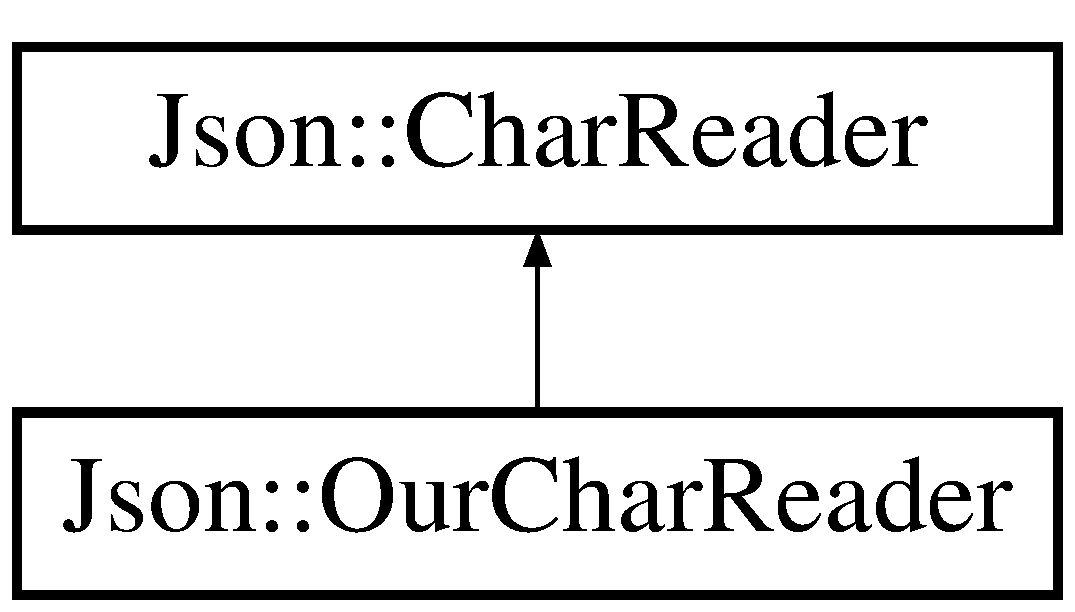
\includegraphics[height=2.000000cm]{classJson_1_1OurCharReader}
\end{center}
\end{figure}
\subsection*{Public Member Functions}
\begin{DoxyCompactItemize}
\item 
\mbox{\Hypertarget{classJson_1_1OurCharReader_a5015506620e7ba7bab417756fa1ca9fe}\label{classJson_1_1OurCharReader_a5015506620e7ba7bab417756fa1ca9fe}} 
{\bfseries Our\+Char\+Reader} (bool collect\+Comments, \hyperlink{classJson_1_1OurFeatures}{Our\+Features} const \&features)
\item 
bool \hyperlink{classJson_1_1OurCharReader_a547f08ec5a9951ca69e8bb2e90296c83}{parse} (char const $\ast$begin\+Doc, char const $\ast$end\+Doc, \hyperlink{classJson_1_1Value}{Value} $\ast$root, J\+S\+O\+N\+C\+P\+P\+\_\+\+S\+T\+R\+I\+NG $\ast$errs) J\+S\+O\+N\+C\+P\+P\+\_\+\+O\+V\+E\+R\+R\+I\+DE
\begin{DoxyCompactList}\small\item\em Read a \hyperlink{classJson_1_1Value}{Value} from a \href{http://www.json.org}{\tt J\+S\+ON} document. The document must be a U\+T\+F-\/8 encoded string containing the document to read. \end{DoxyCompactList}\end{DoxyCompactItemize}


\subsection{Member Function Documentation}
\mbox{\Hypertarget{classJson_1_1OurCharReader_a547f08ec5a9951ca69e8bb2e90296c83}\label{classJson_1_1OurCharReader_a547f08ec5a9951ca69e8bb2e90296c83}} 
\index{Json\+::\+Our\+Char\+Reader@{Json\+::\+Our\+Char\+Reader}!parse@{parse}}
\index{parse@{parse}!Json\+::\+Our\+Char\+Reader@{Json\+::\+Our\+Char\+Reader}}
\subsubsection{\texorpdfstring{parse()}{parse()}}
{\footnotesize\ttfamily bool Json\+::\+Our\+Char\+Reader\+::parse (\begin{DoxyParamCaption}\item[{char const $\ast$}]{begin\+Doc,  }\item[{char const $\ast$}]{end\+Doc,  }\item[{\hyperlink{classJson_1_1Value}{Value} $\ast$}]{root,  }\item[{J\+S\+O\+N\+C\+P\+P\+\_\+\+S\+T\+R\+I\+NG $\ast$}]{errs }\end{DoxyParamCaption})\hspace{0.3cm}{\ttfamily [inline]}, {\ttfamily [virtual]}}



Read a \hyperlink{classJson_1_1Value}{Value} from a \href{http://www.json.org}{\tt J\+S\+ON} document. The document must be a U\+T\+F-\/8 encoded string containing the document to read. 


\begin{DoxyParams}{Parameters}
{\em begin\+Doc} & Pointer on the beginning of the U\+T\+F-\/8 encoded string of the document to read. \\
\hline
{\em end\+Doc} & Pointer on the end of the U\+T\+F-\/8 encoded string of the document to read. Must be $>$= begin\+Doc. \\
\hline
{\em root} & \mbox{[}out\mbox{]} Contains the root value of the document if it was successfully parsed. \\
\hline
{\em errs} & \mbox{[}out\mbox{]} Formatted error messages (if not N\+U\+LL) a user friendly string that lists errors in the parsed document. \\
\hline
\end{DoxyParams}
\begin{DoxyReturn}{Returns}
{\ttfamily true} if the document was successfully parsed, {\ttfamily false} if an error occurred. 
\end{DoxyReturn}


Implements \hyperlink{classJson_1_1CharReader_a7983680d50fd0745f371c43b162e78e1}{Json\+::\+Char\+Reader}.



The documentation for this class was generated from the following file\+:\begin{DoxyCompactItemize}
\item 
jsoncpp.\+cpp\end{DoxyCompactItemize}

\hypertarget{classJson_1_1OurFeatures}{}\section{Json\+:\+:Our\+Features Class Reference}
\label{classJson_1_1OurFeatures}\index{Json\+::\+Our\+Features@{Json\+::\+Our\+Features}}
\subsection*{Static Public Member Functions}
\begin{DoxyCompactItemize}
\item 
\mbox{\Hypertarget{classJson_1_1OurFeatures_a0686e1406b6677f496529f9f3fe98d1e}\label{classJson_1_1OurFeatures_a0686e1406b6677f496529f9f3fe98d1e}} 
static \hyperlink{classJson_1_1OurFeatures}{Our\+Features} {\bfseries all} ()
\end{DoxyCompactItemize}
\subsection*{Public Attributes}
\begin{DoxyCompactItemize}
\item 
\mbox{\Hypertarget{classJson_1_1OurFeatures_ac71bb7ba7363d3b05ed76602b036ce33}\label{classJson_1_1OurFeatures_ac71bb7ba7363d3b05ed76602b036ce33}} 
bool {\bfseries allow\+Comments\+\_\+}
\item 
\mbox{\Hypertarget{classJson_1_1OurFeatures_a2095f66a776c0a4ae6cc931a0c94242e}\label{classJson_1_1OurFeatures_a2095f66a776c0a4ae6cc931a0c94242e}} 
bool {\bfseries strict\+Root\+\_\+}
\item 
\mbox{\Hypertarget{classJson_1_1OurFeatures_a13963bc44bf948eec1968f7ff8e8f5f1}\label{classJson_1_1OurFeatures_a13963bc44bf948eec1968f7ff8e8f5f1}} 
bool {\bfseries allow\+Dropped\+Null\+Placeholders\+\_\+}
\item 
\mbox{\Hypertarget{classJson_1_1OurFeatures_af6973fc7e774ce2d634ba99442aeb91a}\label{classJson_1_1OurFeatures_af6973fc7e774ce2d634ba99442aeb91a}} 
bool {\bfseries allow\+Numeric\+Keys\+\_\+}
\item 
\mbox{\Hypertarget{classJson_1_1OurFeatures_abbd6c196d7a22e2a360a59887eda4610}\label{classJson_1_1OurFeatures_abbd6c196d7a22e2a360a59887eda4610}} 
bool {\bfseries allow\+Single\+Quotes\+\_\+}
\item 
\mbox{\Hypertarget{classJson_1_1OurFeatures_ae8ad25b90706c78f1a8fe929191ac61b}\label{classJson_1_1OurFeatures_ae8ad25b90706c78f1a8fe929191ac61b}} 
bool {\bfseries fail\+If\+Extra\+\_\+}
\item 
\mbox{\Hypertarget{classJson_1_1OurFeatures_a39b8e0b86b1c24a45e800c023bb715aa}\label{classJson_1_1OurFeatures_a39b8e0b86b1c24a45e800c023bb715aa}} 
bool {\bfseries reject\+Dup\+Keys\+\_\+}
\item 
\mbox{\Hypertarget{classJson_1_1OurFeatures_af760f91cc2a7af37e44f78fb466061bb}\label{classJson_1_1OurFeatures_af760f91cc2a7af37e44f78fb466061bb}} 
bool {\bfseries allow\+Special\+Floats\+\_\+}
\item 
\mbox{\Hypertarget{classJson_1_1OurFeatures_a9a786713902d14be6d57a08cc03ccfff}\label{classJson_1_1OurFeatures_a9a786713902d14be6d57a08cc03ccfff}} 
int {\bfseries stack\+Limit\+\_\+}
\end{DoxyCompactItemize}


The documentation for this class was generated from the following file\+:\begin{DoxyCompactItemize}
\item 
jsoncpp.\+cpp\end{DoxyCompactItemize}

\hypertarget{classJson_1_1OurReader}{}\section{Json\+:\+:Our\+Reader Class Reference}
\label{classJson_1_1OurReader}\index{Json\+::\+Our\+Reader@{Json\+::\+Our\+Reader}}
\subsection*{Classes}
\begin{DoxyCompactItemize}
\item 
class \hyperlink{classJson_1_1OurReader_1_1ErrorInfo}{Error\+Info}
\item 
struct \hyperlink{structJson_1_1OurReader_1_1StructuredError}{Structured\+Error}
\item 
class \hyperlink{classJson_1_1OurReader_1_1Token}{Token}
\end{DoxyCompactItemize}
\subsection*{Public Types}
\begin{DoxyCompactItemize}
\item 
typedef char \hyperlink{classJson_1_1OurReader_a0cd0bab4caa66594ab843ccd5f9dc239_a0cd0bab4caa66594ab843ccd5f9dc239}{Char}
\item 
typedef const \hyperlink{classJson_1_1OurReader_a0cd0bab4caa66594ab843ccd5f9dc239_a0cd0bab4caa66594ab843ccd5f9dc239}{Char} $\ast$ \hyperlink{classJson_1_1OurReader_a1bdc7bbc52ba87cae6b19746f2ee0189_a1bdc7bbc52ba87cae6b19746f2ee0189}{Location}
\end{DoxyCompactItemize}
\subsection*{Public Member Functions}
\begin{DoxyCompactItemize}
\item 
\hyperlink{classJson_1_1OurReader_a48a850914b9c8d7781be172930c478e5_a48a850914b9c8d7781be172930c478e5}{Our\+Reader} (\hyperlink{classJson_1_1OurFeatures}{Our\+Features} const \&features)
\item 
bool \hyperlink{classJson_1_1OurReader_aba4f8749aab7f02ec17f107e392caf80_aba4f8749aab7f02ec17f107e392caf80}{parse} (const char $\ast$begin\+Doc, const char $\ast$end\+Doc, \hyperlink{classJson_1_1Value}{Value} \&root, bool collect\+Comments=true)
\item 
\hyperlink{json_8h_a1e723f95759de062585bc4a8fd3fa4be_a1e723f95759de062585bc4a8fd3fa4be}{J\+S\+O\+N\+C\+P\+P\+\_\+\+S\+T\+R\+I\+NG} \hyperlink{classJson_1_1OurReader_a7971de51d73bb4aee5b0c4742c4aaaac_a7971de51d73bb4aee5b0c4742c4aaaac}{get\+Formatted\+Error\+Messages} () const
\item 
std\+::vector$<$ \hyperlink{structJson_1_1OurReader_1_1StructuredError}{Structured\+Error} $>$ \hyperlink{classJson_1_1OurReader_a0eb2420a6bef89a3f3256191e6e3de6d_a0eb2420a6bef89a3f3256191e6e3de6d}{get\+Structured\+Errors} () const
\item 
bool \hyperlink{classJson_1_1OurReader_a700e9d8e0977fa7e0375d26690d7025f_a700e9d8e0977fa7e0375d26690d7025f}{push\+Error} (const \hyperlink{classJson_1_1Value}{Value} \&value, const \hyperlink{json_8h_a1e723f95759de062585bc4a8fd3fa4be_a1e723f95759de062585bc4a8fd3fa4be}{J\+S\+O\+N\+C\+P\+P\+\_\+\+S\+T\+R\+I\+NG} \&message)
\item 
bool \hyperlink{classJson_1_1OurReader_addccecfca74b79adaad6115ddd614477_addccecfca74b79adaad6115ddd614477}{push\+Error} (const \hyperlink{classJson_1_1Value}{Value} \&value, const \hyperlink{json_8h_a1e723f95759de062585bc4a8fd3fa4be_a1e723f95759de062585bc4a8fd3fa4be}{J\+S\+O\+N\+C\+P\+P\+\_\+\+S\+T\+R\+I\+NG} \&message, const \hyperlink{classJson_1_1Value}{Value} \&extra)
\item 
bool \hyperlink{classJson_1_1OurReader_a63c7d874fa379397e0a5fa65f0843845_a63c7d874fa379397e0a5fa65f0843845}{good} () const
\end{DoxyCompactItemize}
\subsection*{Private Types}
\begin{DoxyCompactItemize}
\item 
enum \hyperlink{classJson_1_1OurReader_a15116f7276ddf1e7a2cc3cbefa884dcc_a15116f7276ddf1e7a2cc3cbefa884dcc}{Token\+Type} \{ \newline
\hyperlink{classJson_1_1OurReader_a15116f7276ddf1e7a2cc3cbefa884dcc_a15116f7276ddf1e7a2cc3cbefa884dcca735d1f76eafc2c0c581ed79c077aaa7e}{token\+End\+Of\+Stream} = 0, 
\hyperlink{classJson_1_1OurReader_a15116f7276ddf1e7a2cc3cbefa884dcc_a15116f7276ddf1e7a2cc3cbefa884dcca7495ef5c356d4faa39b702e528cc7e26}{token\+Object\+Begin}, 
\hyperlink{classJson_1_1OurReader_a15116f7276ddf1e7a2cc3cbefa884dcc_a15116f7276ddf1e7a2cc3cbefa884dcca8d7e94be97d76ea1c314130b5aabb014}{token\+Object\+End}, 
\hyperlink{classJson_1_1OurReader_a15116f7276ddf1e7a2cc3cbefa884dcc_a15116f7276ddf1e7a2cc3cbefa884dcca45d229fce2f5f4b52dc0d6c39c853436}{token\+Array\+Begin}, 
\newline
\hyperlink{classJson_1_1OurReader_a15116f7276ddf1e7a2cc3cbefa884dcc_a15116f7276ddf1e7a2cc3cbefa884dcca59a4f42b50d9731dce6be41818c3d91b}{token\+Array\+End}, 
\hyperlink{classJson_1_1OurReader_a15116f7276ddf1e7a2cc3cbefa884dcc_a15116f7276ddf1e7a2cc3cbefa884dccadb37e59e1e52cd5e7417bc418b611ce1}{token\+String}, 
\hyperlink{classJson_1_1OurReader_a15116f7276ddf1e7a2cc3cbefa884dcc_a15116f7276ddf1e7a2cc3cbefa884dcca766aefde855b1246d89b8552240c70d1}{token\+Number}, 
\hyperlink{classJson_1_1OurReader_a15116f7276ddf1e7a2cc3cbefa884dcc_a15116f7276ddf1e7a2cc3cbefa884dccac7d2a552afcea291d47cf49dfefaf619}{token\+True}, 
\newline
\hyperlink{classJson_1_1OurReader_a15116f7276ddf1e7a2cc3cbefa884dcc_a15116f7276ddf1e7a2cc3cbefa884dccaab91e3ef98c1cb1326c3674e518c5126}{token\+False}, 
\hyperlink{classJson_1_1OurReader_a15116f7276ddf1e7a2cc3cbefa884dcc_a15116f7276ddf1e7a2cc3cbefa884dcca4c80b7bb245e3863e38dc8e8586b3c51}{token\+Null}, 
\hyperlink{classJson_1_1OurReader_a15116f7276ddf1e7a2cc3cbefa884dcc_a15116f7276ddf1e7a2cc3cbefa884dcca167898478691f1ac7a240981ccaa1713}{token\+NaN}, 
\hyperlink{classJson_1_1OurReader_a15116f7276ddf1e7a2cc3cbefa884dcc_a15116f7276ddf1e7a2cc3cbefa884dcca800c7c7e896d569ebf6c2771eecc7060}{token\+Pos\+Inf}, 
\newline
\hyperlink{classJson_1_1OurReader_a15116f7276ddf1e7a2cc3cbefa884dcc_a15116f7276ddf1e7a2cc3cbefa884dcca3cf3c4c72d6b5969f17f043a34b2ad4c}{token\+Neg\+Inf}, 
\hyperlink{classJson_1_1OurReader_a15116f7276ddf1e7a2cc3cbefa884dcc_a15116f7276ddf1e7a2cc3cbefa884dcca8ca62ab9091b149d52ec55828f8040f4}{token\+Array\+Separator}, 
\hyperlink{classJson_1_1OurReader_a15116f7276ddf1e7a2cc3cbefa884dcc_a15116f7276ddf1e7a2cc3cbefa884dcca7c95881fb1162316bce42c629bf06214}{token\+Member\+Separator}, 
\hyperlink{classJson_1_1OurReader_a15116f7276ddf1e7a2cc3cbefa884dcc_a15116f7276ddf1e7a2cc3cbefa884dcca777fb6589fdbe225bc10a1e49a090da9}{token\+Comment}, 
\newline
\hyperlink{classJson_1_1OurReader_a15116f7276ddf1e7a2cc3cbefa884dcc_a15116f7276ddf1e7a2cc3cbefa884dccad39f929b971de8dc55fe84a2d2e3465e}{token\+Error}
 \}
\item 
typedef std\+::deque$<$ \hyperlink{classJson_1_1OurReader_1_1ErrorInfo}{Error\+Info} $>$ \hyperlink{classJson_1_1OurReader_a8cc69593ef7303e58e99bb5dbb767562_a8cc69593ef7303e58e99bb5dbb767562}{Errors}
\item 
typedef std\+::stack$<$ \hyperlink{classJson_1_1Value}{Value} $\ast$ $>$ \hyperlink{classJson_1_1OurReader_a8480a5ef159cee3a090f96358414d8d3_a8480a5ef159cee3a090f96358414d8d3}{Nodes}
\end{DoxyCompactItemize}
\subsection*{Private Member Functions}
\begin{DoxyCompactItemize}
\item 
\hyperlink{classJson_1_1OurReader_aee013005522c0d34d2e14962851487ac_aee013005522c0d34d2e14962851487ac}{Our\+Reader} (\hyperlink{classJson_1_1OurReader}{Our\+Reader} const \&)
\item 
void \hyperlink{classJson_1_1OurReader_ad418de7c47bd3d0510888e22110b796e_ad418de7c47bd3d0510888e22110b796e}{operator=} (\hyperlink{classJson_1_1OurReader}{Our\+Reader} const \&)
\item 
bool \hyperlink{classJson_1_1OurReader_a0d1e66da47fe2e85f5033c59326dfdc3_a0d1e66da47fe2e85f5033c59326dfdc3}{read\+Token} (\hyperlink{classJson_1_1OurReader_1_1Token}{Token} \&token)
\item 
void \hyperlink{classJson_1_1OurReader_a6fbc6d58a4505e5ccadf330b57b17ca5_a6fbc6d58a4505e5ccadf330b57b17ca5}{skip\+Spaces} ()
\item 
bool \hyperlink{classJson_1_1OurReader_a4a03f1b266def9b47c4fef35386557fb_a4a03f1b266def9b47c4fef35386557fb}{match} (\hyperlink{classJson_1_1OurReader_a1bdc7bbc52ba87cae6b19746f2ee0189_a1bdc7bbc52ba87cae6b19746f2ee0189}{Location} pattern, int pattern\+Length)
\item 
bool \hyperlink{classJson_1_1OurReader_a90f6bb9e55b2bc3d6c1880809495c222_a90f6bb9e55b2bc3d6c1880809495c222}{read\+Comment} ()
\item 
bool \hyperlink{classJson_1_1OurReader_aba784b125baa1b62387e767b791f2f89_aba784b125baa1b62387e767b791f2f89}{read\+C\+Style\+Comment} ()
\item 
bool \hyperlink{classJson_1_1OurReader_ae3de80671f0f997053e1c1c8a47a45c5_ae3de80671f0f997053e1c1c8a47a45c5}{read\+Cpp\+Style\+Comment} ()
\item 
bool \hyperlink{classJson_1_1OurReader_a5d39b12671499ec5975f3bbc84b7d438_a5d39b12671499ec5975f3bbc84b7d438}{read\+String} ()
\item 
bool \hyperlink{classJson_1_1OurReader_ac78592defdc333faf56c6d0908758da3_ac78592defdc333faf56c6d0908758da3}{read\+String\+Single\+Quote} ()
\item 
bool \hyperlink{classJson_1_1OurReader_aefcb9a78cc45870ccac2db2a66c8ec50_aefcb9a78cc45870ccac2db2a66c8ec50}{read\+Number} (bool check\+Inf)
\item 
bool \hyperlink{classJson_1_1OurReader_a1765d9670d191c89a57a22ea5591d35f_a1765d9670d191c89a57a22ea5591d35f}{read\+Value} ()
\item 
bool \hyperlink{classJson_1_1OurReader_aea198f8101dba55099f4d8121a993530_aea198f8101dba55099f4d8121a993530}{read\+Object} (\hyperlink{classJson_1_1OurReader_1_1Token}{Token} \&token)
\item 
bool \hyperlink{classJson_1_1OurReader_a0b9f58faf4212c6ecb5d8e2a1ac10257_a0b9f58faf4212c6ecb5d8e2a1ac10257}{read\+Array} (\hyperlink{classJson_1_1OurReader_1_1Token}{Token} \&token)
\item 
bool \hyperlink{classJson_1_1OurReader_a272d271290933a89abfd5096dd69c9e9_a272d271290933a89abfd5096dd69c9e9}{decode\+Number} (\hyperlink{classJson_1_1OurReader_1_1Token}{Token} \&token)
\item 
bool \hyperlink{classJson_1_1OurReader_a712270d53a2f023c2f406ac813548340_a712270d53a2f023c2f406ac813548340}{decode\+Number} (\hyperlink{classJson_1_1OurReader_1_1Token}{Token} \&token, \hyperlink{classJson_1_1Value}{Value} \&decoded)
\item 
bool \hyperlink{classJson_1_1OurReader_a34e31d8b8399b7ad493359702b6de6c9_a34e31d8b8399b7ad493359702b6de6c9}{decode\+String} (\hyperlink{classJson_1_1OurReader_1_1Token}{Token} \&token)
\item 
bool \hyperlink{classJson_1_1OurReader_a5046dfa5d43b1770a091aac0a63a9f4b_a5046dfa5d43b1770a091aac0a63a9f4b}{decode\+String} (\hyperlink{classJson_1_1OurReader_1_1Token}{Token} \&token, \hyperlink{json_8h_a1e723f95759de062585bc4a8fd3fa4be_a1e723f95759de062585bc4a8fd3fa4be}{J\+S\+O\+N\+C\+P\+P\+\_\+\+S\+T\+R\+I\+NG} \&decoded)
\item 
bool \hyperlink{classJson_1_1OurReader_a1d1c3b44f6720a0e7c39b5ae8de3981c_a1d1c3b44f6720a0e7c39b5ae8de3981c}{decode\+Double} (\hyperlink{classJson_1_1OurReader_1_1Token}{Token} \&token)
\item 
bool \hyperlink{classJson_1_1OurReader_aa5c15a8cd32754f07430dedba3d1308e_aa5c15a8cd32754f07430dedba3d1308e}{decode\+Double} (\hyperlink{classJson_1_1OurReader_1_1Token}{Token} \&token, \hyperlink{classJson_1_1Value}{Value} \&decoded)
\item 
bool \hyperlink{classJson_1_1OurReader_ac1bf03c161ece082e48da450c50f528d_ac1bf03c161ece082e48da450c50f528d}{decode\+Unicode\+Code\+Point} (\hyperlink{classJson_1_1OurReader_1_1Token}{Token} \&token, \hyperlink{classJson_1_1OurReader_a1bdc7bbc52ba87cae6b19746f2ee0189_a1bdc7bbc52ba87cae6b19746f2ee0189}{Location} \&current, \hyperlink{classJson_1_1OurReader_a1bdc7bbc52ba87cae6b19746f2ee0189_a1bdc7bbc52ba87cae6b19746f2ee0189}{Location} end, unsigned int \&unicode)
\item 
bool \hyperlink{classJson_1_1OurReader_adb39be814cc6076b91a0919bdd5b24b0_adb39be814cc6076b91a0919bdd5b24b0}{decode\+Unicode\+Escape\+Sequence} (\hyperlink{classJson_1_1OurReader_1_1Token}{Token} \&token, \hyperlink{classJson_1_1OurReader_a1bdc7bbc52ba87cae6b19746f2ee0189_a1bdc7bbc52ba87cae6b19746f2ee0189}{Location} \&current, \hyperlink{classJson_1_1OurReader_a1bdc7bbc52ba87cae6b19746f2ee0189_a1bdc7bbc52ba87cae6b19746f2ee0189}{Location} end, unsigned int \&unicode)
\item 
bool \hyperlink{classJson_1_1OurReader_aa6a920311e6408ff3a45324d49da18a6_aa6a920311e6408ff3a45324d49da18a6}{add\+Error} (const \hyperlink{json_8h_a1e723f95759de062585bc4a8fd3fa4be_a1e723f95759de062585bc4a8fd3fa4be}{J\+S\+O\+N\+C\+P\+P\+\_\+\+S\+T\+R\+I\+NG} \&message, \hyperlink{classJson_1_1OurReader_1_1Token}{Token} \&token, \hyperlink{classJson_1_1OurReader_a1bdc7bbc52ba87cae6b19746f2ee0189_a1bdc7bbc52ba87cae6b19746f2ee0189}{Location} extra=0)
\item 
bool \hyperlink{classJson_1_1OurReader_a035651f0700a76a815e5f904c63ebb1c_a035651f0700a76a815e5f904c63ebb1c}{recover\+From\+Error} (\hyperlink{classJson_1_1OurReader_a15116f7276ddf1e7a2cc3cbefa884dcc_a15116f7276ddf1e7a2cc3cbefa884dcc}{Token\+Type} skip\+Until\+Token)
\item 
bool \hyperlink{classJson_1_1OurReader_a074cf3d91e9404fe89e03cfc6a43e6fb_a074cf3d91e9404fe89e03cfc6a43e6fb}{add\+Error\+And\+Recover} (const \hyperlink{json_8h_a1e723f95759de062585bc4a8fd3fa4be_a1e723f95759de062585bc4a8fd3fa4be}{J\+S\+O\+N\+C\+P\+P\+\_\+\+S\+T\+R\+I\+NG} \&message, \hyperlink{classJson_1_1OurReader_1_1Token}{Token} \&token, \hyperlink{classJson_1_1OurReader_a15116f7276ddf1e7a2cc3cbefa884dcc_a15116f7276ddf1e7a2cc3cbefa884dcc}{Token\+Type} skip\+Until\+Token)
\item 
void \hyperlink{classJson_1_1OurReader_ad48bdaf5b686706f003e792fdbcbf102_ad48bdaf5b686706f003e792fdbcbf102}{skip\+Until\+Space} ()
\item 
\hyperlink{classJson_1_1Value}{Value} \& \hyperlink{classJson_1_1OurReader_a2acd5b1d53e7d7e17c21ff8e96edc09d_a2acd5b1d53e7d7e17c21ff8e96edc09d}{current\+Value} ()
\item 
\hyperlink{classJson_1_1OurReader_a0cd0bab4caa66594ab843ccd5f9dc239_a0cd0bab4caa66594ab843ccd5f9dc239}{Char} \hyperlink{classJson_1_1OurReader_a298285d035fdbc554caae09d9f0a5859_a298285d035fdbc554caae09d9f0a5859}{get\+Next\+Char} ()
\item 
void \hyperlink{classJson_1_1OurReader_af482c8e718615646e13a996292e18d74_af482c8e718615646e13a996292e18d74}{get\+Location\+Line\+And\+Column} (\hyperlink{classJson_1_1OurReader_a1bdc7bbc52ba87cae6b19746f2ee0189_a1bdc7bbc52ba87cae6b19746f2ee0189}{Location} location, int \&line, int \&column) const
\item 
\hyperlink{json_8h_a1e723f95759de062585bc4a8fd3fa4be_a1e723f95759de062585bc4a8fd3fa4be}{J\+S\+O\+N\+C\+P\+P\+\_\+\+S\+T\+R\+I\+NG} \hyperlink{classJson_1_1OurReader_ac129e94cdc260822b2fd24e2ca35e636_ac129e94cdc260822b2fd24e2ca35e636}{get\+Location\+Line\+And\+Column} (\hyperlink{classJson_1_1OurReader_a1bdc7bbc52ba87cae6b19746f2ee0189_a1bdc7bbc52ba87cae6b19746f2ee0189}{Location} location) const
\item 
void \hyperlink{classJson_1_1OurReader_ad7318c37469a9106069a236fb4b10e1f_ad7318c37469a9106069a236fb4b10e1f}{add\+Comment} (\hyperlink{classJson_1_1OurReader_a1bdc7bbc52ba87cae6b19746f2ee0189_a1bdc7bbc52ba87cae6b19746f2ee0189}{Location} begin, \hyperlink{classJson_1_1OurReader_a1bdc7bbc52ba87cae6b19746f2ee0189_a1bdc7bbc52ba87cae6b19746f2ee0189}{Location} end, \hyperlink{namespaceJson_a4fc417c23905b2ae9e2c47d197a45351_a4fc417c23905b2ae9e2c47d197a45351}{Comment\+Placement} placement)
\item 
void \hyperlink{classJson_1_1OurReader_a856dea44d92578c276856d7a65a4ebdc_a856dea44d92578c276856d7a65a4ebdc}{skip\+Comment\+Tokens} (\hyperlink{classJson_1_1OurReader_1_1Token}{Token} \&token)
\end{DoxyCompactItemize}
\subsection*{Static Private Member Functions}
\begin{DoxyCompactItemize}
\item 
static \hyperlink{json_8h_a1e723f95759de062585bc4a8fd3fa4be_a1e723f95759de062585bc4a8fd3fa4be}{J\+S\+O\+N\+C\+P\+P\+\_\+\+S\+T\+R\+I\+NG} \hyperlink{classJson_1_1OurReader_a73ec369ee36598e008b80e36263691be_a73ec369ee36598e008b80e36263691be}{normalize\+E\+OL} (\hyperlink{classJson_1_1OurReader_a1bdc7bbc52ba87cae6b19746f2ee0189_a1bdc7bbc52ba87cae6b19746f2ee0189}{Location} begin, \hyperlink{classJson_1_1OurReader_a1bdc7bbc52ba87cae6b19746f2ee0189_a1bdc7bbc52ba87cae6b19746f2ee0189}{Location} end)
\item 
static bool \hyperlink{classJson_1_1OurReader_ab9e83f5a3d9dab2dabce367a4faa2b1b_ab9e83f5a3d9dab2dabce367a4faa2b1b}{contains\+New\+Line} (\hyperlink{classJson_1_1OurReader_a1bdc7bbc52ba87cae6b19746f2ee0189_a1bdc7bbc52ba87cae6b19746f2ee0189}{Location} begin, \hyperlink{classJson_1_1OurReader_a1bdc7bbc52ba87cae6b19746f2ee0189_a1bdc7bbc52ba87cae6b19746f2ee0189}{Location} end)
\end{DoxyCompactItemize}
\subsection*{Private Attributes}
\begin{DoxyCompactItemize}
\item 
\hyperlink{classJson_1_1OurReader_a8480a5ef159cee3a090f96358414d8d3_a8480a5ef159cee3a090f96358414d8d3}{Nodes} \hyperlink{classJson_1_1OurReader_a19cc4e8c5d17ee6822f752e9a36f4ce3_a19cc4e8c5d17ee6822f752e9a36f4ce3}{nodes\+\_\+}
\item 
\hyperlink{classJson_1_1OurReader_a8cc69593ef7303e58e99bb5dbb767562_a8cc69593ef7303e58e99bb5dbb767562}{Errors} \hyperlink{classJson_1_1OurReader_afb76b68ba1ab68fe09cf2838e3d4898d_afb76b68ba1ab68fe09cf2838e3d4898d}{errors\+\_\+}
\item 
\hyperlink{json_8h_a1e723f95759de062585bc4a8fd3fa4be_a1e723f95759de062585bc4a8fd3fa4be}{J\+S\+O\+N\+C\+P\+P\+\_\+\+S\+T\+R\+I\+NG} \hyperlink{classJson_1_1OurReader_a726230af83d22d25e0c76cec3408ecf1_a726230af83d22d25e0c76cec3408ecf1}{document\+\_\+}
\item 
\hyperlink{classJson_1_1OurReader_a1bdc7bbc52ba87cae6b19746f2ee0189_a1bdc7bbc52ba87cae6b19746f2ee0189}{Location} \hyperlink{classJson_1_1OurReader_a9bda9d72335d52cd06e65f9eca3f70f5_a9bda9d72335d52cd06e65f9eca3f70f5}{begin\+\_\+}
\item 
\hyperlink{classJson_1_1OurReader_a1bdc7bbc52ba87cae6b19746f2ee0189_a1bdc7bbc52ba87cae6b19746f2ee0189}{Location} \hyperlink{classJson_1_1OurReader_ab1f69b0260c27a0d2d65dc56e42c8f9d_ab1f69b0260c27a0d2d65dc56e42c8f9d}{end\+\_\+}
\item 
\hyperlink{classJson_1_1OurReader_a1bdc7bbc52ba87cae6b19746f2ee0189_a1bdc7bbc52ba87cae6b19746f2ee0189}{Location} \hyperlink{classJson_1_1OurReader_a5211fbbba94be80a22dd2317c621efcc_a5211fbbba94be80a22dd2317c621efcc}{current\+\_\+}
\item 
\hyperlink{classJson_1_1OurReader_a1bdc7bbc52ba87cae6b19746f2ee0189_a1bdc7bbc52ba87cae6b19746f2ee0189}{Location} \hyperlink{classJson_1_1OurReader_a101eadc45e01c60628b53f0db3d13482_a101eadc45e01c60628b53f0db3d13482}{last\+Value\+End\+\_\+}
\item 
\hyperlink{classJson_1_1Value}{Value} $\ast$ \hyperlink{classJson_1_1OurReader_a9f994b6a2227c5d96e6ed6cbc74ed251_a9f994b6a2227c5d96e6ed6cbc74ed251}{last\+Value\+\_\+}
\item 
\hyperlink{json_8h_a1e723f95759de062585bc4a8fd3fa4be_a1e723f95759de062585bc4a8fd3fa4be}{J\+S\+O\+N\+C\+P\+P\+\_\+\+S\+T\+R\+I\+NG} \hyperlink{classJson_1_1OurReader_a9c53e77e290eb9081298210a955fda6a_a9c53e77e290eb9081298210a955fda6a}{comments\+Before\+\_\+}
\item 
\hyperlink{classJson_1_1OurFeatures}{Our\+Features} const \hyperlink{classJson_1_1OurReader_a2714302d5cc54ca2ce4118ea51c0397a_a2714302d5cc54ca2ce4118ea51c0397a}{features\+\_\+}
\item 
bool \hyperlink{classJson_1_1OurReader_a259f6ac988da2894bcafc670e42f73ad_a259f6ac988da2894bcafc670e42f73ad}{collect\+Comments\+\_\+}
\end{DoxyCompactItemize}


\subsection{Member Typedef Documentation}
\mbox{\Hypertarget{classJson_1_1OurReader_a0cd0bab4caa66594ab843ccd5f9dc239_a0cd0bab4caa66594ab843ccd5f9dc239}\label{classJson_1_1OurReader_a0cd0bab4caa66594ab843ccd5f9dc239_a0cd0bab4caa66594ab843ccd5f9dc239}} 
\index{Json\+::\+Our\+Reader@{Json\+::\+Our\+Reader}!Char@{Char}}
\index{Char@{Char}!Json\+::\+Our\+Reader@{Json\+::\+Our\+Reader}}
\subsubsection{\texorpdfstring{Char}{Char}}
{\footnotesize\ttfamily typedef char \hyperlink{classJson_1_1OurReader_a0cd0bab4caa66594ab843ccd5f9dc239_a0cd0bab4caa66594ab843ccd5f9dc239}{Json\+::\+Our\+Reader\+::\+Char}}

\mbox{\Hypertarget{classJson_1_1OurReader_a8cc69593ef7303e58e99bb5dbb767562_a8cc69593ef7303e58e99bb5dbb767562}\label{classJson_1_1OurReader_a8cc69593ef7303e58e99bb5dbb767562_a8cc69593ef7303e58e99bb5dbb767562}} 
\index{Json\+::\+Our\+Reader@{Json\+::\+Our\+Reader}!Errors@{Errors}}
\index{Errors@{Errors}!Json\+::\+Our\+Reader@{Json\+::\+Our\+Reader}}
\subsubsection{\texorpdfstring{Errors}{Errors}}
{\footnotesize\ttfamily typedef std\+::deque$<$\hyperlink{classJson_1_1OurReader_1_1ErrorInfo}{Error\+Info}$>$ \hyperlink{classJson_1_1OurReader_a8cc69593ef7303e58e99bb5dbb767562_a8cc69593ef7303e58e99bb5dbb767562}{Json\+::\+Our\+Reader\+::\+Errors}\hspace{0.3cm}{\ttfamily [private]}}

\mbox{\Hypertarget{classJson_1_1OurReader_a1bdc7bbc52ba87cae6b19746f2ee0189_a1bdc7bbc52ba87cae6b19746f2ee0189}\label{classJson_1_1OurReader_a1bdc7bbc52ba87cae6b19746f2ee0189_a1bdc7bbc52ba87cae6b19746f2ee0189}} 
\index{Json\+::\+Our\+Reader@{Json\+::\+Our\+Reader}!Location@{Location}}
\index{Location@{Location}!Json\+::\+Our\+Reader@{Json\+::\+Our\+Reader}}
\subsubsection{\texorpdfstring{Location}{Location}}
{\footnotesize\ttfamily typedef const \hyperlink{classJson_1_1OurReader_a0cd0bab4caa66594ab843ccd5f9dc239_a0cd0bab4caa66594ab843ccd5f9dc239}{Char}$\ast$ \hyperlink{classJson_1_1OurReader_a1bdc7bbc52ba87cae6b19746f2ee0189_a1bdc7bbc52ba87cae6b19746f2ee0189}{Json\+::\+Our\+Reader\+::\+Location}}

\mbox{\Hypertarget{classJson_1_1OurReader_a8480a5ef159cee3a090f96358414d8d3_a8480a5ef159cee3a090f96358414d8d3}\label{classJson_1_1OurReader_a8480a5ef159cee3a090f96358414d8d3_a8480a5ef159cee3a090f96358414d8d3}} 
\index{Json\+::\+Our\+Reader@{Json\+::\+Our\+Reader}!Nodes@{Nodes}}
\index{Nodes@{Nodes}!Json\+::\+Our\+Reader@{Json\+::\+Our\+Reader}}
\subsubsection{\texorpdfstring{Nodes}{Nodes}}
{\footnotesize\ttfamily typedef std\+::stack$<$\hyperlink{classJson_1_1Value}{Value}$\ast$$>$ \hyperlink{classJson_1_1OurReader_a8480a5ef159cee3a090f96358414d8d3_a8480a5ef159cee3a090f96358414d8d3}{Json\+::\+Our\+Reader\+::\+Nodes}\hspace{0.3cm}{\ttfamily [private]}}



\subsection{Member Enumeration Documentation}
\mbox{\Hypertarget{classJson_1_1OurReader_a15116f7276ddf1e7a2cc3cbefa884dcc_a15116f7276ddf1e7a2cc3cbefa884dcc}\label{classJson_1_1OurReader_a15116f7276ddf1e7a2cc3cbefa884dcc_a15116f7276ddf1e7a2cc3cbefa884dcc}} 
\index{Json\+::\+Our\+Reader@{Json\+::\+Our\+Reader}!Token\+Type@{Token\+Type}}
\index{Token\+Type@{Token\+Type}!Json\+::\+Our\+Reader@{Json\+::\+Our\+Reader}}
\subsubsection{\texorpdfstring{Token\+Type}{TokenType}}
{\footnotesize\ttfamily enum \hyperlink{classJson_1_1OurReader_a15116f7276ddf1e7a2cc3cbefa884dcc_a15116f7276ddf1e7a2cc3cbefa884dcc}{Json\+::\+Our\+Reader\+::\+Token\+Type}\hspace{0.3cm}{\ttfamily [private]}}

\begin{DoxyEnumFields}{Enumerator}
\raisebox{\heightof{T}}[0pt][0pt]{\index{token\+End\+Of\+Stream@{token\+End\+Of\+Stream}!Json\+::\+Our\+Reader@{Json\+::\+Our\+Reader}}\index{Json\+::\+Our\+Reader@{Json\+::\+Our\+Reader}!token\+End\+Of\+Stream@{token\+End\+Of\+Stream}}}\mbox{\Hypertarget{classJson_1_1OurReader_a15116f7276ddf1e7a2cc3cbefa884dcc_a15116f7276ddf1e7a2cc3cbefa884dcca735d1f76eafc2c0c581ed79c077aaa7e}\label{classJson_1_1OurReader_a15116f7276ddf1e7a2cc3cbefa884dcc_a15116f7276ddf1e7a2cc3cbefa884dcca735d1f76eafc2c0c581ed79c077aaa7e}} 
token\+End\+Of\+Stream&\\
\hline

\raisebox{\heightof{T}}[0pt][0pt]{\index{token\+Object\+Begin@{token\+Object\+Begin}!Json\+::\+Our\+Reader@{Json\+::\+Our\+Reader}}\index{Json\+::\+Our\+Reader@{Json\+::\+Our\+Reader}!token\+Object\+Begin@{token\+Object\+Begin}}}\mbox{\Hypertarget{classJson_1_1OurReader_a15116f7276ddf1e7a2cc3cbefa884dcc_a15116f7276ddf1e7a2cc3cbefa884dcca7495ef5c356d4faa39b702e528cc7e26}\label{classJson_1_1OurReader_a15116f7276ddf1e7a2cc3cbefa884dcc_a15116f7276ddf1e7a2cc3cbefa884dcca7495ef5c356d4faa39b702e528cc7e26}} 
token\+Object\+Begin&\\
\hline

\raisebox{\heightof{T}}[0pt][0pt]{\index{token\+Object\+End@{token\+Object\+End}!Json\+::\+Our\+Reader@{Json\+::\+Our\+Reader}}\index{Json\+::\+Our\+Reader@{Json\+::\+Our\+Reader}!token\+Object\+End@{token\+Object\+End}}}\mbox{\Hypertarget{classJson_1_1OurReader_a15116f7276ddf1e7a2cc3cbefa884dcc_a15116f7276ddf1e7a2cc3cbefa884dcca8d7e94be97d76ea1c314130b5aabb014}\label{classJson_1_1OurReader_a15116f7276ddf1e7a2cc3cbefa884dcc_a15116f7276ddf1e7a2cc3cbefa884dcca8d7e94be97d76ea1c314130b5aabb014}} 
token\+Object\+End&\\
\hline

\raisebox{\heightof{T}}[0pt][0pt]{\index{token\+Array\+Begin@{token\+Array\+Begin}!Json\+::\+Our\+Reader@{Json\+::\+Our\+Reader}}\index{Json\+::\+Our\+Reader@{Json\+::\+Our\+Reader}!token\+Array\+Begin@{token\+Array\+Begin}}}\mbox{\Hypertarget{classJson_1_1OurReader_a15116f7276ddf1e7a2cc3cbefa884dcc_a15116f7276ddf1e7a2cc3cbefa884dcca45d229fce2f5f4b52dc0d6c39c853436}\label{classJson_1_1OurReader_a15116f7276ddf1e7a2cc3cbefa884dcc_a15116f7276ddf1e7a2cc3cbefa884dcca45d229fce2f5f4b52dc0d6c39c853436}} 
token\+Array\+Begin&\\
\hline

\raisebox{\heightof{T}}[0pt][0pt]{\index{token\+Array\+End@{token\+Array\+End}!Json\+::\+Our\+Reader@{Json\+::\+Our\+Reader}}\index{Json\+::\+Our\+Reader@{Json\+::\+Our\+Reader}!token\+Array\+End@{token\+Array\+End}}}\mbox{\Hypertarget{classJson_1_1OurReader_a15116f7276ddf1e7a2cc3cbefa884dcc_a15116f7276ddf1e7a2cc3cbefa884dcca59a4f42b50d9731dce6be41818c3d91b}\label{classJson_1_1OurReader_a15116f7276ddf1e7a2cc3cbefa884dcc_a15116f7276ddf1e7a2cc3cbefa884dcca59a4f42b50d9731dce6be41818c3d91b}} 
token\+Array\+End&\\
\hline

\raisebox{\heightof{T}}[0pt][0pt]{\index{token\+String@{token\+String}!Json\+::\+Our\+Reader@{Json\+::\+Our\+Reader}}\index{Json\+::\+Our\+Reader@{Json\+::\+Our\+Reader}!token\+String@{token\+String}}}\mbox{\Hypertarget{classJson_1_1OurReader_a15116f7276ddf1e7a2cc3cbefa884dcc_a15116f7276ddf1e7a2cc3cbefa884dccadb37e59e1e52cd5e7417bc418b611ce1}\label{classJson_1_1OurReader_a15116f7276ddf1e7a2cc3cbefa884dcc_a15116f7276ddf1e7a2cc3cbefa884dccadb37e59e1e52cd5e7417bc418b611ce1}} 
token\+String&\\
\hline

\raisebox{\heightof{T}}[0pt][0pt]{\index{token\+Number@{token\+Number}!Json\+::\+Our\+Reader@{Json\+::\+Our\+Reader}}\index{Json\+::\+Our\+Reader@{Json\+::\+Our\+Reader}!token\+Number@{token\+Number}}}\mbox{\Hypertarget{classJson_1_1OurReader_a15116f7276ddf1e7a2cc3cbefa884dcc_a15116f7276ddf1e7a2cc3cbefa884dcca766aefde855b1246d89b8552240c70d1}\label{classJson_1_1OurReader_a15116f7276ddf1e7a2cc3cbefa884dcc_a15116f7276ddf1e7a2cc3cbefa884dcca766aefde855b1246d89b8552240c70d1}} 
token\+Number&\\
\hline

\raisebox{\heightof{T}}[0pt][0pt]{\index{token\+True@{token\+True}!Json\+::\+Our\+Reader@{Json\+::\+Our\+Reader}}\index{Json\+::\+Our\+Reader@{Json\+::\+Our\+Reader}!token\+True@{token\+True}}}\mbox{\Hypertarget{classJson_1_1OurReader_a15116f7276ddf1e7a2cc3cbefa884dcc_a15116f7276ddf1e7a2cc3cbefa884dccac7d2a552afcea291d47cf49dfefaf619}\label{classJson_1_1OurReader_a15116f7276ddf1e7a2cc3cbefa884dcc_a15116f7276ddf1e7a2cc3cbefa884dccac7d2a552afcea291d47cf49dfefaf619}} 
token\+True&\\
\hline

\raisebox{\heightof{T}}[0pt][0pt]{\index{token\+False@{token\+False}!Json\+::\+Our\+Reader@{Json\+::\+Our\+Reader}}\index{Json\+::\+Our\+Reader@{Json\+::\+Our\+Reader}!token\+False@{token\+False}}}\mbox{\Hypertarget{classJson_1_1OurReader_a15116f7276ddf1e7a2cc3cbefa884dcc_a15116f7276ddf1e7a2cc3cbefa884dccaab91e3ef98c1cb1326c3674e518c5126}\label{classJson_1_1OurReader_a15116f7276ddf1e7a2cc3cbefa884dcc_a15116f7276ddf1e7a2cc3cbefa884dccaab91e3ef98c1cb1326c3674e518c5126}} 
token\+False&\\
\hline

\raisebox{\heightof{T}}[0pt][0pt]{\index{token\+Null@{token\+Null}!Json\+::\+Our\+Reader@{Json\+::\+Our\+Reader}}\index{Json\+::\+Our\+Reader@{Json\+::\+Our\+Reader}!token\+Null@{token\+Null}}}\mbox{\Hypertarget{classJson_1_1OurReader_a15116f7276ddf1e7a2cc3cbefa884dcc_a15116f7276ddf1e7a2cc3cbefa884dcca4c80b7bb245e3863e38dc8e8586b3c51}\label{classJson_1_1OurReader_a15116f7276ddf1e7a2cc3cbefa884dcc_a15116f7276ddf1e7a2cc3cbefa884dcca4c80b7bb245e3863e38dc8e8586b3c51}} 
token\+Null&\\
\hline

\raisebox{\heightof{T}}[0pt][0pt]{\index{token\+NaN@{token\+NaN}!Json\+::\+Our\+Reader@{Json\+::\+Our\+Reader}}\index{Json\+::\+Our\+Reader@{Json\+::\+Our\+Reader}!token\+NaN@{token\+NaN}}}\mbox{\Hypertarget{classJson_1_1OurReader_a15116f7276ddf1e7a2cc3cbefa884dcc_a15116f7276ddf1e7a2cc3cbefa884dcca167898478691f1ac7a240981ccaa1713}\label{classJson_1_1OurReader_a15116f7276ddf1e7a2cc3cbefa884dcc_a15116f7276ddf1e7a2cc3cbefa884dcca167898478691f1ac7a240981ccaa1713}} 
token\+NaN&\\
\hline

\raisebox{\heightof{T}}[0pt][0pt]{\index{token\+Pos\+Inf@{token\+Pos\+Inf}!Json\+::\+Our\+Reader@{Json\+::\+Our\+Reader}}\index{Json\+::\+Our\+Reader@{Json\+::\+Our\+Reader}!token\+Pos\+Inf@{token\+Pos\+Inf}}}\mbox{\Hypertarget{classJson_1_1OurReader_a15116f7276ddf1e7a2cc3cbefa884dcc_a15116f7276ddf1e7a2cc3cbefa884dcca800c7c7e896d569ebf6c2771eecc7060}\label{classJson_1_1OurReader_a15116f7276ddf1e7a2cc3cbefa884dcc_a15116f7276ddf1e7a2cc3cbefa884dcca800c7c7e896d569ebf6c2771eecc7060}} 
token\+Pos\+Inf&\\
\hline

\raisebox{\heightof{T}}[0pt][0pt]{\index{token\+Neg\+Inf@{token\+Neg\+Inf}!Json\+::\+Our\+Reader@{Json\+::\+Our\+Reader}}\index{Json\+::\+Our\+Reader@{Json\+::\+Our\+Reader}!token\+Neg\+Inf@{token\+Neg\+Inf}}}\mbox{\Hypertarget{classJson_1_1OurReader_a15116f7276ddf1e7a2cc3cbefa884dcc_a15116f7276ddf1e7a2cc3cbefa884dcca3cf3c4c72d6b5969f17f043a34b2ad4c}\label{classJson_1_1OurReader_a15116f7276ddf1e7a2cc3cbefa884dcc_a15116f7276ddf1e7a2cc3cbefa884dcca3cf3c4c72d6b5969f17f043a34b2ad4c}} 
token\+Neg\+Inf&\\
\hline

\raisebox{\heightof{T}}[0pt][0pt]{\index{token\+Array\+Separator@{token\+Array\+Separator}!Json\+::\+Our\+Reader@{Json\+::\+Our\+Reader}}\index{Json\+::\+Our\+Reader@{Json\+::\+Our\+Reader}!token\+Array\+Separator@{token\+Array\+Separator}}}\mbox{\Hypertarget{classJson_1_1OurReader_a15116f7276ddf1e7a2cc3cbefa884dcc_a15116f7276ddf1e7a2cc3cbefa884dcca8ca62ab9091b149d52ec55828f8040f4}\label{classJson_1_1OurReader_a15116f7276ddf1e7a2cc3cbefa884dcc_a15116f7276ddf1e7a2cc3cbefa884dcca8ca62ab9091b149d52ec55828f8040f4}} 
token\+Array\+Separator&\\
\hline

\raisebox{\heightof{T}}[0pt][0pt]{\index{token\+Member\+Separator@{token\+Member\+Separator}!Json\+::\+Our\+Reader@{Json\+::\+Our\+Reader}}\index{Json\+::\+Our\+Reader@{Json\+::\+Our\+Reader}!token\+Member\+Separator@{token\+Member\+Separator}}}\mbox{\Hypertarget{classJson_1_1OurReader_a15116f7276ddf1e7a2cc3cbefa884dcc_a15116f7276ddf1e7a2cc3cbefa884dcca7c95881fb1162316bce42c629bf06214}\label{classJson_1_1OurReader_a15116f7276ddf1e7a2cc3cbefa884dcc_a15116f7276ddf1e7a2cc3cbefa884dcca7c95881fb1162316bce42c629bf06214}} 
token\+Member\+Separator&\\
\hline

\raisebox{\heightof{T}}[0pt][0pt]{\index{token\+Comment@{token\+Comment}!Json\+::\+Our\+Reader@{Json\+::\+Our\+Reader}}\index{Json\+::\+Our\+Reader@{Json\+::\+Our\+Reader}!token\+Comment@{token\+Comment}}}\mbox{\Hypertarget{classJson_1_1OurReader_a15116f7276ddf1e7a2cc3cbefa884dcc_a15116f7276ddf1e7a2cc3cbefa884dcca777fb6589fdbe225bc10a1e49a090da9}\label{classJson_1_1OurReader_a15116f7276ddf1e7a2cc3cbefa884dcc_a15116f7276ddf1e7a2cc3cbefa884dcca777fb6589fdbe225bc10a1e49a090da9}} 
token\+Comment&\\
\hline

\raisebox{\heightof{T}}[0pt][0pt]{\index{token\+Error@{token\+Error}!Json\+::\+Our\+Reader@{Json\+::\+Our\+Reader}}\index{Json\+::\+Our\+Reader@{Json\+::\+Our\+Reader}!token\+Error@{token\+Error}}}\mbox{\Hypertarget{classJson_1_1OurReader_a15116f7276ddf1e7a2cc3cbefa884dcc_a15116f7276ddf1e7a2cc3cbefa884dccad39f929b971de8dc55fe84a2d2e3465e}\label{classJson_1_1OurReader_a15116f7276ddf1e7a2cc3cbefa884dcc_a15116f7276ddf1e7a2cc3cbefa884dccad39f929b971de8dc55fe84a2d2e3465e}} 
token\+Error&\\
\hline

\end{DoxyEnumFields}


\subsection{Constructor \& Destructor Documentation}
\mbox{\Hypertarget{classJson_1_1OurReader_a48a850914b9c8d7781be172930c478e5_a48a850914b9c8d7781be172930c478e5}\label{classJson_1_1OurReader_a48a850914b9c8d7781be172930c478e5_a48a850914b9c8d7781be172930c478e5}} 
\index{Json\+::\+Our\+Reader@{Json\+::\+Our\+Reader}!Our\+Reader@{Our\+Reader}}
\index{Our\+Reader@{Our\+Reader}!Json\+::\+Our\+Reader@{Json\+::\+Our\+Reader}}
\subsubsection{\texorpdfstring{Our\+Reader()}{OurReader()}\hspace{0.1cm}{\footnotesize\ttfamily [1/2]}}
{\footnotesize\ttfamily Json\+::\+Our\+Reader\+::\+Our\+Reader (\begin{DoxyParamCaption}\item[{\hyperlink{classJson_1_1OurFeatures}{Our\+Features} const \&}]{features }\end{DoxyParamCaption})}

\mbox{\Hypertarget{classJson_1_1OurReader_aee013005522c0d34d2e14962851487ac_aee013005522c0d34d2e14962851487ac}\label{classJson_1_1OurReader_aee013005522c0d34d2e14962851487ac_aee013005522c0d34d2e14962851487ac}} 
\index{Json\+::\+Our\+Reader@{Json\+::\+Our\+Reader}!Our\+Reader@{Our\+Reader}}
\index{Our\+Reader@{Our\+Reader}!Json\+::\+Our\+Reader@{Json\+::\+Our\+Reader}}
\subsubsection{\texorpdfstring{Our\+Reader()}{OurReader()}\hspace{0.1cm}{\footnotesize\ttfamily [2/2]}}
{\footnotesize\ttfamily Json\+::\+Our\+Reader\+::\+Our\+Reader (\begin{DoxyParamCaption}\item[{\hyperlink{classJson_1_1OurReader}{Our\+Reader} const \&}]{ }\end{DoxyParamCaption})\hspace{0.3cm}{\ttfamily [private]}}



\subsection{Member Function Documentation}
\mbox{\Hypertarget{classJson_1_1OurReader_ad7318c37469a9106069a236fb4b10e1f_ad7318c37469a9106069a236fb4b10e1f}\label{classJson_1_1OurReader_ad7318c37469a9106069a236fb4b10e1f_ad7318c37469a9106069a236fb4b10e1f}} 
\index{Json\+::\+Our\+Reader@{Json\+::\+Our\+Reader}!add\+Comment@{add\+Comment}}
\index{add\+Comment@{add\+Comment}!Json\+::\+Our\+Reader@{Json\+::\+Our\+Reader}}
\subsubsection{\texorpdfstring{add\+Comment()}{addComment()}}
{\footnotesize\ttfamily void Json\+::\+Our\+Reader\+::add\+Comment (\begin{DoxyParamCaption}\item[{\hyperlink{classJson_1_1OurReader_a1bdc7bbc52ba87cae6b19746f2ee0189_a1bdc7bbc52ba87cae6b19746f2ee0189}{Location}}]{begin,  }\item[{\hyperlink{classJson_1_1OurReader_a1bdc7bbc52ba87cae6b19746f2ee0189_a1bdc7bbc52ba87cae6b19746f2ee0189}{Location}}]{end,  }\item[{\hyperlink{namespaceJson_a4fc417c23905b2ae9e2c47d197a45351_a4fc417c23905b2ae9e2c47d197a45351}{Comment\+Placement}}]{placement }\end{DoxyParamCaption})\hspace{0.3cm}{\ttfamily [private]}}



References collect\+Comments\+\_\+, Json\+::comment\+After\+On\+Same\+Line, comments\+Before\+\_\+, J\+S\+O\+N\+C\+P\+P\+\_\+\+S\+T\+R\+I\+NG, last\+Value\+\_\+, normalize\+E\+O\+L(), and Json\+::\+Value\+::set\+Comment().



Referenced by read\+Comment().

\mbox{\Hypertarget{classJson_1_1OurReader_aa6a920311e6408ff3a45324d49da18a6_aa6a920311e6408ff3a45324d49da18a6}\label{classJson_1_1OurReader_aa6a920311e6408ff3a45324d49da18a6_aa6a920311e6408ff3a45324d49da18a6}} 
\index{Json\+::\+Our\+Reader@{Json\+::\+Our\+Reader}!add\+Error@{add\+Error}}
\index{add\+Error@{add\+Error}!Json\+::\+Our\+Reader@{Json\+::\+Our\+Reader}}
\subsubsection{\texorpdfstring{add\+Error()}{addError()}}
{\footnotesize\ttfamily bool Json\+::\+Our\+Reader\+::add\+Error (\begin{DoxyParamCaption}\item[{const \hyperlink{json_8h_a1e723f95759de062585bc4a8fd3fa4be_a1e723f95759de062585bc4a8fd3fa4be}{J\+S\+O\+N\+C\+P\+P\+\_\+\+S\+T\+R\+I\+NG} \&}]{message,  }\item[{\hyperlink{classJson_1_1OurReader_1_1Token}{Token} \&}]{token,  }\item[{\hyperlink{classJson_1_1OurReader_a1bdc7bbc52ba87cae6b19746f2ee0189_a1bdc7bbc52ba87cae6b19746f2ee0189}{Location}}]{extra = {\ttfamily 0} }\end{DoxyParamCaption})\hspace{0.3cm}{\ttfamily [private]}}



References errors\+\_\+, Json\+::\+Our\+Reader\+::\+Error\+Info\+::extra\+\_\+, Json\+::\+Our\+Reader\+::\+Error\+Info\+::message\+\_\+, and Json\+::\+Our\+Reader\+::\+Error\+Info\+::token\+\_\+.



Referenced by add\+Error\+And\+Recover(), decode\+Double(), decode\+String(), decode\+Unicode\+Code\+Point(), decode\+Unicode\+Escape\+Sequence(), parse(), and read\+Value().

\mbox{\Hypertarget{classJson_1_1OurReader_a074cf3d91e9404fe89e03cfc6a43e6fb_a074cf3d91e9404fe89e03cfc6a43e6fb}\label{classJson_1_1OurReader_a074cf3d91e9404fe89e03cfc6a43e6fb_a074cf3d91e9404fe89e03cfc6a43e6fb}} 
\index{Json\+::\+Our\+Reader@{Json\+::\+Our\+Reader}!add\+Error\+And\+Recover@{add\+Error\+And\+Recover}}
\index{add\+Error\+And\+Recover@{add\+Error\+And\+Recover}!Json\+::\+Our\+Reader@{Json\+::\+Our\+Reader}}
\subsubsection{\texorpdfstring{add\+Error\+And\+Recover()}{addErrorAndRecover()}}
{\footnotesize\ttfamily bool Json\+::\+Our\+Reader\+::add\+Error\+And\+Recover (\begin{DoxyParamCaption}\item[{const \hyperlink{json_8h_a1e723f95759de062585bc4a8fd3fa4be_a1e723f95759de062585bc4a8fd3fa4be}{J\+S\+O\+N\+C\+P\+P\+\_\+\+S\+T\+R\+I\+NG} \&}]{message,  }\item[{\hyperlink{classJson_1_1OurReader_1_1Token}{Token} \&}]{token,  }\item[{\hyperlink{classJson_1_1OurReader_a15116f7276ddf1e7a2cc3cbefa884dcc_a15116f7276ddf1e7a2cc3cbefa884dcc}{Token\+Type}}]{skip\+Until\+Token }\end{DoxyParamCaption})\hspace{0.3cm}{\ttfamily [private]}}



References add\+Error(), and recover\+From\+Error().



Referenced by read\+Array(), and read\+Object().

\mbox{\Hypertarget{classJson_1_1OurReader_ab9e83f5a3d9dab2dabce367a4faa2b1b_ab9e83f5a3d9dab2dabce367a4faa2b1b}\label{classJson_1_1OurReader_ab9e83f5a3d9dab2dabce367a4faa2b1b_ab9e83f5a3d9dab2dabce367a4faa2b1b}} 
\index{Json\+::\+Our\+Reader@{Json\+::\+Our\+Reader}!contains\+New\+Line@{contains\+New\+Line}}
\index{contains\+New\+Line@{contains\+New\+Line}!Json\+::\+Our\+Reader@{Json\+::\+Our\+Reader}}
\subsubsection{\texorpdfstring{contains\+New\+Line()}{containsNewLine()}}
{\footnotesize\ttfamily bool Json\+::\+Our\+Reader\+::contains\+New\+Line (\begin{DoxyParamCaption}\item[{\hyperlink{classJson_1_1OurReader_a1bdc7bbc52ba87cae6b19746f2ee0189_a1bdc7bbc52ba87cae6b19746f2ee0189}{Our\+Reader\+::\+Location}}]{begin,  }\item[{\hyperlink{classJson_1_1OurReader_a1bdc7bbc52ba87cae6b19746f2ee0189_a1bdc7bbc52ba87cae6b19746f2ee0189}{Our\+Reader\+::\+Location}}]{end }\end{DoxyParamCaption})\hspace{0.3cm}{\ttfamily [static]}, {\ttfamily [private]}}



Referenced by read\+Comment().

\mbox{\Hypertarget{classJson_1_1OurReader_a2acd5b1d53e7d7e17c21ff8e96edc09d_a2acd5b1d53e7d7e17c21ff8e96edc09d}\label{classJson_1_1OurReader_a2acd5b1d53e7d7e17c21ff8e96edc09d_a2acd5b1d53e7d7e17c21ff8e96edc09d}} 
\index{Json\+::\+Our\+Reader@{Json\+::\+Our\+Reader}!current\+Value@{current\+Value}}
\index{current\+Value@{current\+Value}!Json\+::\+Our\+Reader@{Json\+::\+Our\+Reader}}
\subsubsection{\texorpdfstring{current\+Value()}{currentValue()}}
{\footnotesize\ttfamily \hyperlink{classJson_1_1Value}{Value} \& Json\+::\+Our\+Reader\+::current\+Value (\begin{DoxyParamCaption}{ }\end{DoxyParamCaption})\hspace{0.3cm}{\ttfamily [private]}}



References nodes\+\_\+.



Referenced by decode\+Double(), decode\+Number(), decode\+String(), read\+Array(), read\+Object(), and read\+Value().

\mbox{\Hypertarget{classJson_1_1OurReader_a1d1c3b44f6720a0e7c39b5ae8de3981c_a1d1c3b44f6720a0e7c39b5ae8de3981c}\label{classJson_1_1OurReader_a1d1c3b44f6720a0e7c39b5ae8de3981c_a1d1c3b44f6720a0e7c39b5ae8de3981c}} 
\index{Json\+::\+Our\+Reader@{Json\+::\+Our\+Reader}!decode\+Double@{decode\+Double}}
\index{decode\+Double@{decode\+Double}!Json\+::\+Our\+Reader@{Json\+::\+Our\+Reader}}
\subsubsection{\texorpdfstring{decode\+Double()}{decodeDouble()}\hspace{0.1cm}{\footnotesize\ttfamily [1/2]}}
{\footnotesize\ttfamily bool Json\+::\+Our\+Reader\+::decode\+Double (\begin{DoxyParamCaption}\item[{\hyperlink{classJson_1_1OurReader_1_1Token}{Token} \&}]{token }\end{DoxyParamCaption})\hspace{0.3cm}{\ttfamily [private]}}



References begin\+\_\+, current\+Value(), Json\+::\+Our\+Reader\+::\+Token\+::end\+\_\+, Json\+::\+Value\+::set\+Offset\+Limit(), Json\+::\+Value\+::set\+Offset\+Start(), Json\+::\+Our\+Reader\+::\+Token\+::start\+\_\+, and Json\+::\+Value\+::swap\+Payload().



Referenced by decode\+Number().

\mbox{\Hypertarget{classJson_1_1OurReader_aa5c15a8cd32754f07430dedba3d1308e_aa5c15a8cd32754f07430dedba3d1308e}\label{classJson_1_1OurReader_aa5c15a8cd32754f07430dedba3d1308e_aa5c15a8cd32754f07430dedba3d1308e}} 
\index{Json\+::\+Our\+Reader@{Json\+::\+Our\+Reader}!decode\+Double@{decode\+Double}}
\index{decode\+Double@{decode\+Double}!Json\+::\+Our\+Reader@{Json\+::\+Our\+Reader}}
\subsubsection{\texorpdfstring{decode\+Double()}{decodeDouble()}\hspace{0.1cm}{\footnotesize\ttfamily [2/2]}}
{\footnotesize\ttfamily bool Json\+::\+Our\+Reader\+::decode\+Double (\begin{DoxyParamCaption}\item[{\hyperlink{classJson_1_1OurReader_1_1Token}{Token} \&}]{token,  }\item[{\hyperlink{classJson_1_1Value}{Value} \&}]{decoded }\end{DoxyParamCaption})\hspace{0.3cm}{\ttfamily [private]}}



References add\+Error(), Json\+::\+Our\+Reader\+::\+Token\+::end\+\_\+, Json\+::fix\+Numeric\+Locale\+Input(), J\+S\+O\+N\+C\+P\+P\+\_\+\+S\+T\+R\+I\+NG, and Json\+::\+Our\+Reader\+::\+Token\+::start\+\_\+.

\mbox{\Hypertarget{classJson_1_1OurReader_a272d271290933a89abfd5096dd69c9e9_a272d271290933a89abfd5096dd69c9e9}\label{classJson_1_1OurReader_a272d271290933a89abfd5096dd69c9e9_a272d271290933a89abfd5096dd69c9e9}} 
\index{Json\+::\+Our\+Reader@{Json\+::\+Our\+Reader}!decode\+Number@{decode\+Number}}
\index{decode\+Number@{decode\+Number}!Json\+::\+Our\+Reader@{Json\+::\+Our\+Reader}}
\subsubsection{\texorpdfstring{decode\+Number()}{decodeNumber()}\hspace{0.1cm}{\footnotesize\ttfamily [1/2]}}
{\footnotesize\ttfamily bool Json\+::\+Our\+Reader\+::decode\+Number (\begin{DoxyParamCaption}\item[{\hyperlink{classJson_1_1OurReader_1_1Token}{Token} \&}]{token }\end{DoxyParamCaption})\hspace{0.3cm}{\ttfamily [private]}}



References begin\+\_\+, current\+Value(), Json\+::\+Our\+Reader\+::\+Token\+::end\+\_\+, Json\+::\+Value\+::set\+Offset\+Limit(), Json\+::\+Value\+::set\+Offset\+Start(), Json\+::\+Our\+Reader\+::\+Token\+::start\+\_\+, and Json\+::\+Value\+::swap\+Payload().



Referenced by read\+Object(), and read\+Value().

\mbox{\Hypertarget{classJson_1_1OurReader_a712270d53a2f023c2f406ac813548340_a712270d53a2f023c2f406ac813548340}\label{classJson_1_1OurReader_a712270d53a2f023c2f406ac813548340_a712270d53a2f023c2f406ac813548340}} 
\index{Json\+::\+Our\+Reader@{Json\+::\+Our\+Reader}!decode\+Number@{decode\+Number}}
\index{decode\+Number@{decode\+Number}!Json\+::\+Our\+Reader@{Json\+::\+Our\+Reader}}
\subsubsection{\texorpdfstring{decode\+Number()}{decodeNumber()}\hspace{0.1cm}{\footnotesize\ttfamily [2/2]}}
{\footnotesize\ttfamily bool Json\+::\+Our\+Reader\+::decode\+Number (\begin{DoxyParamCaption}\item[{\hyperlink{classJson_1_1OurReader_1_1Token}{Token} \&}]{token,  }\item[{\hyperlink{classJson_1_1Value}{Value} \&}]{decoded }\end{DoxyParamCaption})\hspace{0.3cm}{\ttfamily [private]}}



References decode\+Double(), Json\+::\+Our\+Reader\+::\+Token\+::end\+\_\+, Json\+::\+Value\+::max\+Int, Json\+::\+Value\+::max\+Largest\+U\+Int, Json\+::\+Value\+::min\+Largest\+Int, and Json\+::\+Our\+Reader\+::\+Token\+::start\+\_\+.

\mbox{\Hypertarget{classJson_1_1OurReader_a34e31d8b8399b7ad493359702b6de6c9_a34e31d8b8399b7ad493359702b6de6c9}\label{classJson_1_1OurReader_a34e31d8b8399b7ad493359702b6de6c9_a34e31d8b8399b7ad493359702b6de6c9}} 
\index{Json\+::\+Our\+Reader@{Json\+::\+Our\+Reader}!decode\+String@{decode\+String}}
\index{decode\+String@{decode\+String}!Json\+::\+Our\+Reader@{Json\+::\+Our\+Reader}}
\subsubsection{\texorpdfstring{decode\+String()}{decodeString()}\hspace{0.1cm}{\footnotesize\ttfamily [1/2]}}
{\footnotesize\ttfamily bool Json\+::\+Our\+Reader\+::decode\+String (\begin{DoxyParamCaption}\item[{\hyperlink{classJson_1_1OurReader_1_1Token}{Token} \&}]{token }\end{DoxyParamCaption})\hspace{0.3cm}{\ttfamily [private]}}



References begin\+\_\+, current\+Value(), Json\+::\+Our\+Reader\+::\+Token\+::end\+\_\+, J\+S\+O\+N\+C\+P\+P\+\_\+\+S\+T\+R\+I\+NG, Json\+::\+Value\+::set\+Offset\+Limit(), Json\+::\+Value\+::set\+Offset\+Start(), Json\+::\+Our\+Reader\+::\+Token\+::start\+\_\+, and Json\+::\+Value\+::swap\+Payload().



Referenced by read\+Object(), and read\+Value().

\mbox{\Hypertarget{classJson_1_1OurReader_a5046dfa5d43b1770a091aac0a63a9f4b_a5046dfa5d43b1770a091aac0a63a9f4b}\label{classJson_1_1OurReader_a5046dfa5d43b1770a091aac0a63a9f4b_a5046dfa5d43b1770a091aac0a63a9f4b}} 
\index{Json\+::\+Our\+Reader@{Json\+::\+Our\+Reader}!decode\+String@{decode\+String}}
\index{decode\+String@{decode\+String}!Json\+::\+Our\+Reader@{Json\+::\+Our\+Reader}}
\subsubsection{\texorpdfstring{decode\+String()}{decodeString()}\hspace{0.1cm}{\footnotesize\ttfamily [2/2]}}
{\footnotesize\ttfamily bool Json\+::\+Our\+Reader\+::decode\+String (\begin{DoxyParamCaption}\item[{\hyperlink{classJson_1_1OurReader_1_1Token}{Token} \&}]{token,  }\item[{\hyperlink{json_8h_a1e723f95759de062585bc4a8fd3fa4be_a1e723f95759de062585bc4a8fd3fa4be}{J\+S\+O\+N\+C\+P\+P\+\_\+\+S\+T\+R\+I\+NG} \&}]{decoded }\end{DoxyParamCaption})\hspace{0.3cm}{\ttfamily [private]}}



References add\+Error(), Json\+::code\+Point\+To\+U\+T\+F8(), decode\+Unicode\+Code\+Point(), Json\+::\+Our\+Reader\+::\+Token\+::end\+\_\+, and Json\+::\+Our\+Reader\+::\+Token\+::start\+\_\+.

\mbox{\Hypertarget{classJson_1_1OurReader_ac1bf03c161ece082e48da450c50f528d_ac1bf03c161ece082e48da450c50f528d}\label{classJson_1_1OurReader_ac1bf03c161ece082e48da450c50f528d_ac1bf03c161ece082e48da450c50f528d}} 
\index{Json\+::\+Our\+Reader@{Json\+::\+Our\+Reader}!decode\+Unicode\+Code\+Point@{decode\+Unicode\+Code\+Point}}
\index{decode\+Unicode\+Code\+Point@{decode\+Unicode\+Code\+Point}!Json\+::\+Our\+Reader@{Json\+::\+Our\+Reader}}
\subsubsection{\texorpdfstring{decode\+Unicode\+Code\+Point()}{decodeUnicodeCodePoint()}}
{\footnotesize\ttfamily bool Json\+::\+Our\+Reader\+::decode\+Unicode\+Code\+Point (\begin{DoxyParamCaption}\item[{\hyperlink{classJson_1_1OurReader_1_1Token}{Token} \&}]{token,  }\item[{\hyperlink{classJson_1_1OurReader_a1bdc7bbc52ba87cae6b19746f2ee0189_a1bdc7bbc52ba87cae6b19746f2ee0189}{Location} \&}]{current,  }\item[{\hyperlink{classJson_1_1OurReader_a1bdc7bbc52ba87cae6b19746f2ee0189_a1bdc7bbc52ba87cae6b19746f2ee0189}{Location}}]{end,  }\item[{unsigned int \&}]{unicode }\end{DoxyParamCaption})\hspace{0.3cm}{\ttfamily [private]}}



References add\+Error(), and decode\+Unicode\+Escape\+Sequence().



Referenced by decode\+String().

\mbox{\Hypertarget{classJson_1_1OurReader_adb39be814cc6076b91a0919bdd5b24b0_adb39be814cc6076b91a0919bdd5b24b0}\label{classJson_1_1OurReader_adb39be814cc6076b91a0919bdd5b24b0_adb39be814cc6076b91a0919bdd5b24b0}} 
\index{Json\+::\+Our\+Reader@{Json\+::\+Our\+Reader}!decode\+Unicode\+Escape\+Sequence@{decode\+Unicode\+Escape\+Sequence}}
\index{decode\+Unicode\+Escape\+Sequence@{decode\+Unicode\+Escape\+Sequence}!Json\+::\+Our\+Reader@{Json\+::\+Our\+Reader}}
\subsubsection{\texorpdfstring{decode\+Unicode\+Escape\+Sequence()}{decodeUnicodeEscapeSequence()}}
{\footnotesize\ttfamily bool Json\+::\+Our\+Reader\+::decode\+Unicode\+Escape\+Sequence (\begin{DoxyParamCaption}\item[{\hyperlink{classJson_1_1OurReader_1_1Token}{Token} \&}]{token,  }\item[{\hyperlink{classJson_1_1OurReader_a1bdc7bbc52ba87cae6b19746f2ee0189_a1bdc7bbc52ba87cae6b19746f2ee0189}{Location} \&}]{current,  }\item[{\hyperlink{classJson_1_1OurReader_a1bdc7bbc52ba87cae6b19746f2ee0189_a1bdc7bbc52ba87cae6b19746f2ee0189}{Location}}]{end,  }\item[{unsigned int \&}]{unicode }\end{DoxyParamCaption})\hspace{0.3cm}{\ttfamily [private]}}



References add\+Error().



Referenced by decode\+Unicode\+Code\+Point().

\mbox{\Hypertarget{classJson_1_1OurReader_a7971de51d73bb4aee5b0c4742c4aaaac_a7971de51d73bb4aee5b0c4742c4aaaac}\label{classJson_1_1OurReader_a7971de51d73bb4aee5b0c4742c4aaaac_a7971de51d73bb4aee5b0c4742c4aaaac}} 
\index{Json\+::\+Our\+Reader@{Json\+::\+Our\+Reader}!get\+Formatted\+Error\+Messages@{get\+Formatted\+Error\+Messages}}
\index{get\+Formatted\+Error\+Messages@{get\+Formatted\+Error\+Messages}!Json\+::\+Our\+Reader@{Json\+::\+Our\+Reader}}
\subsubsection{\texorpdfstring{get\+Formatted\+Error\+Messages()}{getFormattedErrorMessages()}}
{\footnotesize\ttfamily \hyperlink{json_8h_a1e723f95759de062585bc4a8fd3fa4be_a1e723f95759de062585bc4a8fd3fa4be}{J\+S\+O\+N\+C\+P\+P\+\_\+\+S\+T\+R\+I\+NG} Json\+::\+Our\+Reader\+::get\+Formatted\+Error\+Messages (\begin{DoxyParamCaption}{ }\end{DoxyParamCaption}) const}



References errors\+\_\+, Json\+::\+Our\+Reader\+::\+Error\+Info\+::extra\+\_\+, get\+Location\+Line\+And\+Column(), J\+S\+O\+N\+C\+P\+P\+\_\+\+S\+T\+R\+I\+NG, Json\+::\+Our\+Reader\+::\+Error\+Info\+::message\+\_\+, Json\+::\+Our\+Reader\+::\+Token\+::start\+\_\+, and Json\+::\+Our\+Reader\+::\+Error\+Info\+::token\+\_\+.



Referenced by Json\+::\+Our\+Char\+Reader\+::parse().

\mbox{\Hypertarget{classJson_1_1OurReader_af482c8e718615646e13a996292e18d74_af482c8e718615646e13a996292e18d74}\label{classJson_1_1OurReader_af482c8e718615646e13a996292e18d74_af482c8e718615646e13a996292e18d74}} 
\index{Json\+::\+Our\+Reader@{Json\+::\+Our\+Reader}!get\+Location\+Line\+And\+Column@{get\+Location\+Line\+And\+Column}}
\index{get\+Location\+Line\+And\+Column@{get\+Location\+Line\+And\+Column}!Json\+::\+Our\+Reader@{Json\+::\+Our\+Reader}}
\subsubsection{\texorpdfstring{get\+Location\+Line\+And\+Column()}{getLocationLineAndColumn()}\hspace{0.1cm}{\footnotesize\ttfamily [1/2]}}
{\footnotesize\ttfamily void Json\+::\+Our\+Reader\+::get\+Location\+Line\+And\+Column (\begin{DoxyParamCaption}\item[{\hyperlink{classJson_1_1OurReader_a1bdc7bbc52ba87cae6b19746f2ee0189_a1bdc7bbc52ba87cae6b19746f2ee0189}{Location}}]{location,  }\item[{int \&}]{line,  }\item[{int \&}]{column }\end{DoxyParamCaption}) const\hspace{0.3cm}{\ttfamily [private]}}



References begin\+\_\+, and end\+\_\+.



Referenced by get\+Formatted\+Error\+Messages(), and get\+Location\+Line\+And\+Column().

\mbox{\Hypertarget{classJson_1_1OurReader_ac129e94cdc260822b2fd24e2ca35e636_ac129e94cdc260822b2fd24e2ca35e636}\label{classJson_1_1OurReader_ac129e94cdc260822b2fd24e2ca35e636_ac129e94cdc260822b2fd24e2ca35e636}} 
\index{Json\+::\+Our\+Reader@{Json\+::\+Our\+Reader}!get\+Location\+Line\+And\+Column@{get\+Location\+Line\+And\+Column}}
\index{get\+Location\+Line\+And\+Column@{get\+Location\+Line\+And\+Column}!Json\+::\+Our\+Reader@{Json\+::\+Our\+Reader}}
\subsubsection{\texorpdfstring{get\+Location\+Line\+And\+Column()}{getLocationLineAndColumn()}\hspace{0.1cm}{\footnotesize\ttfamily [2/2]}}
{\footnotesize\ttfamily \hyperlink{json_8h_a1e723f95759de062585bc4a8fd3fa4be_a1e723f95759de062585bc4a8fd3fa4be}{J\+S\+O\+N\+C\+P\+P\+\_\+\+S\+T\+R\+I\+NG} Json\+::\+Our\+Reader\+::get\+Location\+Line\+And\+Column (\begin{DoxyParamCaption}\item[{\hyperlink{classJson_1_1OurReader_a1bdc7bbc52ba87cae6b19746f2ee0189_a1bdc7bbc52ba87cae6b19746f2ee0189}{Location}}]{location }\end{DoxyParamCaption}) const\hspace{0.3cm}{\ttfamily [private]}}



References get\+Location\+Line\+And\+Column().

\mbox{\Hypertarget{classJson_1_1OurReader_a298285d035fdbc554caae09d9f0a5859_a298285d035fdbc554caae09d9f0a5859}\label{classJson_1_1OurReader_a298285d035fdbc554caae09d9f0a5859_a298285d035fdbc554caae09d9f0a5859}} 
\index{Json\+::\+Our\+Reader@{Json\+::\+Our\+Reader}!get\+Next\+Char@{get\+Next\+Char}}
\index{get\+Next\+Char@{get\+Next\+Char}!Json\+::\+Our\+Reader@{Json\+::\+Our\+Reader}}
\subsubsection{\texorpdfstring{get\+Next\+Char()}{getNextChar()}}
{\footnotesize\ttfamily \hyperlink{classJson_1_1OurReader_a0cd0bab4caa66594ab843ccd5f9dc239_a0cd0bab4caa66594ab843ccd5f9dc239}{Our\+Reader\+::\+Char} Json\+::\+Our\+Reader\+::get\+Next\+Char (\begin{DoxyParamCaption}{ }\end{DoxyParamCaption})\hspace{0.3cm}{\ttfamily [private]}}



References current\+\_\+, and end\+\_\+.



Referenced by read\+Comment(), read\+Cpp\+Style\+Comment(), read\+C\+Style\+Comment(), read\+String(), read\+String\+Single\+Quote(), and read\+Token().

\mbox{\Hypertarget{classJson_1_1OurReader_a0eb2420a6bef89a3f3256191e6e3de6d_a0eb2420a6bef89a3f3256191e6e3de6d}\label{classJson_1_1OurReader_a0eb2420a6bef89a3f3256191e6e3de6d_a0eb2420a6bef89a3f3256191e6e3de6d}} 
\index{Json\+::\+Our\+Reader@{Json\+::\+Our\+Reader}!get\+Structured\+Errors@{get\+Structured\+Errors}}
\index{get\+Structured\+Errors@{get\+Structured\+Errors}!Json\+::\+Our\+Reader@{Json\+::\+Our\+Reader}}
\subsubsection{\texorpdfstring{get\+Structured\+Errors()}{getStructuredErrors()}}
{\footnotesize\ttfamily std\+::vector$<$ \hyperlink{structJson_1_1OurReader_1_1StructuredError}{Our\+Reader\+::\+Structured\+Error} $>$ Json\+::\+Our\+Reader\+::get\+Structured\+Errors (\begin{DoxyParamCaption}{ }\end{DoxyParamCaption}) const}



References begin\+\_\+, Json\+::\+Our\+Reader\+::\+Token\+::end\+\_\+, errors\+\_\+, Json\+::\+Our\+Reader\+::\+Structured\+Error\+::message, Json\+::\+Our\+Reader\+::\+Error\+Info\+::message\+\_\+, Json\+::\+Our\+Reader\+::\+Structured\+Error\+::offset\+\_\+limit, Json\+::\+Our\+Reader\+::\+Structured\+Error\+::offset\+\_\+start, Json\+::\+Our\+Reader\+::\+Token\+::start\+\_\+, and Json\+::\+Our\+Reader\+::\+Error\+Info\+::token\+\_\+.

\mbox{\Hypertarget{classJson_1_1OurReader_a63c7d874fa379397e0a5fa65f0843845_a63c7d874fa379397e0a5fa65f0843845}\label{classJson_1_1OurReader_a63c7d874fa379397e0a5fa65f0843845_a63c7d874fa379397e0a5fa65f0843845}} 
\index{Json\+::\+Our\+Reader@{Json\+::\+Our\+Reader}!good@{good}}
\index{good@{good}!Json\+::\+Our\+Reader@{Json\+::\+Our\+Reader}}
\subsubsection{\texorpdfstring{good()}{good()}}
{\footnotesize\ttfamily bool Json\+::\+Our\+Reader\+::good (\begin{DoxyParamCaption}{ }\end{DoxyParamCaption}) const}



References errors\+\_\+.

\mbox{\Hypertarget{classJson_1_1OurReader_a4a03f1b266def9b47c4fef35386557fb_a4a03f1b266def9b47c4fef35386557fb}\label{classJson_1_1OurReader_a4a03f1b266def9b47c4fef35386557fb_a4a03f1b266def9b47c4fef35386557fb}} 
\index{Json\+::\+Our\+Reader@{Json\+::\+Our\+Reader}!match@{match}}
\index{match@{match}!Json\+::\+Our\+Reader@{Json\+::\+Our\+Reader}}
\subsubsection{\texorpdfstring{match()}{match()}}
{\footnotesize\ttfamily bool Json\+::\+Our\+Reader\+::match (\begin{DoxyParamCaption}\item[{\hyperlink{classJson_1_1OurReader_a1bdc7bbc52ba87cae6b19746f2ee0189_a1bdc7bbc52ba87cae6b19746f2ee0189}{Location}}]{pattern,  }\item[{int}]{pattern\+Length }\end{DoxyParamCaption})\hspace{0.3cm}{\ttfamily [private]}}



References current\+\_\+, and end\+\_\+.



Referenced by read\+Token().

\mbox{\Hypertarget{classJson_1_1OurReader_a73ec369ee36598e008b80e36263691be_a73ec369ee36598e008b80e36263691be}\label{classJson_1_1OurReader_a73ec369ee36598e008b80e36263691be_a73ec369ee36598e008b80e36263691be}} 
\index{Json\+::\+Our\+Reader@{Json\+::\+Our\+Reader}!normalize\+E\+OL@{normalize\+E\+OL}}
\index{normalize\+E\+OL@{normalize\+E\+OL}!Json\+::\+Our\+Reader@{Json\+::\+Our\+Reader}}
\subsubsection{\texorpdfstring{normalize\+E\+O\+L()}{normalizeEOL()}}
{\footnotesize\ttfamily \hyperlink{json_8h_a1e723f95759de062585bc4a8fd3fa4be_a1e723f95759de062585bc4a8fd3fa4be}{J\+S\+O\+N\+C\+P\+P\+\_\+\+S\+T\+R\+I\+NG} Json\+::\+Our\+Reader\+::normalize\+E\+OL (\begin{DoxyParamCaption}\item[{\hyperlink{classJson_1_1OurReader_a1bdc7bbc52ba87cae6b19746f2ee0189_a1bdc7bbc52ba87cae6b19746f2ee0189}{Our\+Reader\+::\+Location}}]{begin,  }\item[{\hyperlink{classJson_1_1OurReader_a1bdc7bbc52ba87cae6b19746f2ee0189_a1bdc7bbc52ba87cae6b19746f2ee0189}{Our\+Reader\+::\+Location}}]{end }\end{DoxyParamCaption})\hspace{0.3cm}{\ttfamily [static]}, {\ttfamily [private]}}



References J\+S\+O\+N\+C\+P\+P\+\_\+\+S\+T\+R\+I\+NG.



Referenced by add\+Comment().

\mbox{\Hypertarget{classJson_1_1OurReader_ad418de7c47bd3d0510888e22110b796e_ad418de7c47bd3d0510888e22110b796e}\label{classJson_1_1OurReader_ad418de7c47bd3d0510888e22110b796e_ad418de7c47bd3d0510888e22110b796e}} 
\index{Json\+::\+Our\+Reader@{Json\+::\+Our\+Reader}!operator=@{operator=}}
\index{operator=@{operator=}!Json\+::\+Our\+Reader@{Json\+::\+Our\+Reader}}
\subsubsection{\texorpdfstring{operator=()}{operator=()}}
{\footnotesize\ttfamily void Json\+::\+Our\+Reader\+::operator= (\begin{DoxyParamCaption}\item[{\hyperlink{classJson_1_1OurReader}{Our\+Reader} const \&}]{ }\end{DoxyParamCaption})\hspace{0.3cm}{\ttfamily [private]}}

\mbox{\Hypertarget{classJson_1_1OurReader_aba4f8749aab7f02ec17f107e392caf80_aba4f8749aab7f02ec17f107e392caf80}\label{classJson_1_1OurReader_aba4f8749aab7f02ec17f107e392caf80_aba4f8749aab7f02ec17f107e392caf80}} 
\index{Json\+::\+Our\+Reader@{Json\+::\+Our\+Reader}!parse@{parse}}
\index{parse@{parse}!Json\+::\+Our\+Reader@{Json\+::\+Our\+Reader}}
\subsubsection{\texorpdfstring{parse()}{parse()}}
{\footnotesize\ttfamily bool Json\+::\+Our\+Reader\+::parse (\begin{DoxyParamCaption}\item[{const char $\ast$}]{begin\+Doc,  }\item[{const char $\ast$}]{end\+Doc,  }\item[{\hyperlink{classJson_1_1Value}{Value} \&}]{root,  }\item[{bool}]{collect\+Comments = {\ttfamily true} }\end{DoxyParamCaption})}



References add\+Error(), Json\+::\+Our\+Features\+::allow\+Comments\+\_\+, begin\+\_\+, collect\+Comments\+\_\+, Json\+::comment\+After, comments\+Before\+\_\+, current\+\_\+, Json\+::\+Our\+Reader\+::\+Token\+::end\+\_\+, end\+\_\+, errors\+\_\+, Json\+::\+Our\+Features\+::fail\+If\+Extra\+\_\+, features\+\_\+, Json\+::\+Value\+::is\+Array(), Json\+::\+Value\+::is\+Object(), last\+Value\+\_\+, last\+Value\+End\+\_\+, nodes\+\_\+, read\+Value(), Json\+::\+Value\+::set\+Comment(), skip\+Comment\+Tokens(), Json\+::\+Our\+Reader\+::\+Token\+::start\+\_\+, Json\+::\+Our\+Features\+::strict\+Root\+\_\+, token\+End\+Of\+Stream, token\+Error, and Json\+::\+Our\+Reader\+::\+Token\+::type\+\_\+.



Referenced by Json\+::\+Our\+Char\+Reader\+::parse().

\mbox{\Hypertarget{classJson_1_1OurReader_a700e9d8e0977fa7e0375d26690d7025f_a700e9d8e0977fa7e0375d26690d7025f}\label{classJson_1_1OurReader_a700e9d8e0977fa7e0375d26690d7025f_a700e9d8e0977fa7e0375d26690d7025f}} 
\index{Json\+::\+Our\+Reader@{Json\+::\+Our\+Reader}!push\+Error@{push\+Error}}
\index{push\+Error@{push\+Error}!Json\+::\+Our\+Reader@{Json\+::\+Our\+Reader}}
\subsubsection{\texorpdfstring{push\+Error()}{pushError()}\hspace{0.1cm}{\footnotesize\ttfamily [1/2]}}
{\footnotesize\ttfamily bool Json\+::\+Our\+Reader\+::push\+Error (\begin{DoxyParamCaption}\item[{const \hyperlink{classJson_1_1Value}{Value} \&}]{value,  }\item[{const \hyperlink{json_8h_a1e723f95759de062585bc4a8fd3fa4be_a1e723f95759de062585bc4a8fd3fa4be}{J\+S\+O\+N\+C\+P\+P\+\_\+\+S\+T\+R\+I\+NG} \&}]{message }\end{DoxyParamCaption})}



References begin\+\_\+, Json\+::\+Our\+Reader\+::\+Token\+::end\+\_\+, end\+\_\+, errors\+\_\+, Json\+::\+Our\+Reader\+::\+Error\+Info\+::extra\+\_\+, Json\+::\+Value\+::get\+Offset\+Limit(), Json\+::\+Value\+::get\+Offset\+Start(), Json\+::\+Our\+Reader\+::\+Error\+Info\+::message\+\_\+, Json\+::\+Our\+Reader\+::\+Token\+::start\+\_\+, Json\+::\+Our\+Reader\+::\+Error\+Info\+::token\+\_\+, token\+Error, and Json\+::\+Our\+Reader\+::\+Token\+::type\+\_\+.

\mbox{\Hypertarget{classJson_1_1OurReader_addccecfca74b79adaad6115ddd614477_addccecfca74b79adaad6115ddd614477}\label{classJson_1_1OurReader_addccecfca74b79adaad6115ddd614477_addccecfca74b79adaad6115ddd614477}} 
\index{Json\+::\+Our\+Reader@{Json\+::\+Our\+Reader}!push\+Error@{push\+Error}}
\index{push\+Error@{push\+Error}!Json\+::\+Our\+Reader@{Json\+::\+Our\+Reader}}
\subsubsection{\texorpdfstring{push\+Error()}{pushError()}\hspace{0.1cm}{\footnotesize\ttfamily [2/2]}}
{\footnotesize\ttfamily bool Json\+::\+Our\+Reader\+::push\+Error (\begin{DoxyParamCaption}\item[{const \hyperlink{classJson_1_1Value}{Value} \&}]{value,  }\item[{const \hyperlink{json_8h_a1e723f95759de062585bc4a8fd3fa4be_a1e723f95759de062585bc4a8fd3fa4be}{J\+S\+O\+N\+C\+P\+P\+\_\+\+S\+T\+R\+I\+NG} \&}]{message,  }\item[{const \hyperlink{classJson_1_1Value}{Value} \&}]{extra }\end{DoxyParamCaption})}



References begin\+\_\+, Json\+::\+Our\+Reader\+::\+Token\+::end\+\_\+, end\+\_\+, errors\+\_\+, Json\+::\+Our\+Reader\+::\+Error\+Info\+::extra\+\_\+, Json\+::\+Value\+::get\+Offset\+Limit(), Json\+::\+Value\+::get\+Offset\+Start(), Json\+::\+Our\+Reader\+::\+Error\+Info\+::message\+\_\+, Json\+::\+Our\+Reader\+::\+Token\+::start\+\_\+, Json\+::\+Our\+Reader\+::\+Error\+Info\+::token\+\_\+, token\+Error, and Json\+::\+Our\+Reader\+::\+Token\+::type\+\_\+.

\mbox{\Hypertarget{classJson_1_1OurReader_a0b9f58faf4212c6ecb5d8e2a1ac10257_a0b9f58faf4212c6ecb5d8e2a1ac10257}\label{classJson_1_1OurReader_a0b9f58faf4212c6ecb5d8e2a1ac10257_a0b9f58faf4212c6ecb5d8e2a1ac10257}} 
\index{Json\+::\+Our\+Reader@{Json\+::\+Our\+Reader}!read\+Array@{read\+Array}}
\index{read\+Array@{read\+Array}!Json\+::\+Our\+Reader@{Json\+::\+Our\+Reader}}
\subsubsection{\texorpdfstring{read\+Array()}{readArray()}}
{\footnotesize\ttfamily bool Json\+::\+Our\+Reader\+::read\+Array (\begin{DoxyParamCaption}\item[{\hyperlink{classJson_1_1OurReader_1_1Token}{Token} \&}]{token }\end{DoxyParamCaption})\hspace{0.3cm}{\ttfamily [private]}}



References add\+Error\+And\+Recover(), Json\+::array\+Value, begin\+\_\+, current\+\_\+, current\+Value(), end\+\_\+, nodes\+\_\+, read\+Token(), read\+Value(), recover\+From\+Error(), Json\+::\+Value\+::set\+Offset\+Start(), skip\+Spaces(), Json\+::\+Our\+Reader\+::\+Token\+::start\+\_\+, Json\+::\+Value\+::swap\+Payload(), token\+Array\+End, token\+Array\+Separator, token\+Comment, and Json\+::\+Our\+Reader\+::\+Token\+::type\+\_\+.



Referenced by read\+Value().

\mbox{\Hypertarget{classJson_1_1OurReader_a90f6bb9e55b2bc3d6c1880809495c222_a90f6bb9e55b2bc3d6c1880809495c222}\label{classJson_1_1OurReader_a90f6bb9e55b2bc3d6c1880809495c222_a90f6bb9e55b2bc3d6c1880809495c222}} 
\index{Json\+::\+Our\+Reader@{Json\+::\+Our\+Reader}!read\+Comment@{read\+Comment}}
\index{read\+Comment@{read\+Comment}!Json\+::\+Our\+Reader@{Json\+::\+Our\+Reader}}
\subsubsection{\texorpdfstring{read\+Comment()}{readComment()}}
{\footnotesize\ttfamily bool Json\+::\+Our\+Reader\+::read\+Comment (\begin{DoxyParamCaption}{ }\end{DoxyParamCaption})\hspace{0.3cm}{\ttfamily [private]}}



References add\+Comment(), collect\+Comments\+\_\+, Json\+::comment\+After\+On\+Same\+Line, Json\+::comment\+Before, contains\+New\+Line(), current\+\_\+, get\+Next\+Char(), last\+Value\+End\+\_\+, read\+Cpp\+Style\+Comment(), and read\+C\+Style\+Comment().



Referenced by read\+Token().

\mbox{\Hypertarget{classJson_1_1OurReader_ae3de80671f0f997053e1c1c8a47a45c5_ae3de80671f0f997053e1c1c8a47a45c5}\label{classJson_1_1OurReader_ae3de80671f0f997053e1c1c8a47a45c5_ae3de80671f0f997053e1c1c8a47a45c5}} 
\index{Json\+::\+Our\+Reader@{Json\+::\+Our\+Reader}!read\+Cpp\+Style\+Comment@{read\+Cpp\+Style\+Comment}}
\index{read\+Cpp\+Style\+Comment@{read\+Cpp\+Style\+Comment}!Json\+::\+Our\+Reader@{Json\+::\+Our\+Reader}}
\subsubsection{\texorpdfstring{read\+Cpp\+Style\+Comment()}{readCppStyleComment()}}
{\footnotesize\ttfamily bool Json\+::\+Our\+Reader\+::read\+Cpp\+Style\+Comment (\begin{DoxyParamCaption}{ }\end{DoxyParamCaption})\hspace{0.3cm}{\ttfamily [private]}}



References current\+\_\+, end\+\_\+, and get\+Next\+Char().



Referenced by read\+Comment().

\mbox{\Hypertarget{classJson_1_1OurReader_aba784b125baa1b62387e767b791f2f89_aba784b125baa1b62387e767b791f2f89}\label{classJson_1_1OurReader_aba784b125baa1b62387e767b791f2f89_aba784b125baa1b62387e767b791f2f89}} 
\index{Json\+::\+Our\+Reader@{Json\+::\+Our\+Reader}!read\+C\+Style\+Comment@{read\+C\+Style\+Comment}}
\index{read\+C\+Style\+Comment@{read\+C\+Style\+Comment}!Json\+::\+Our\+Reader@{Json\+::\+Our\+Reader}}
\subsubsection{\texorpdfstring{read\+C\+Style\+Comment()}{readCStyleComment()}}
{\footnotesize\ttfamily bool Json\+::\+Our\+Reader\+::read\+C\+Style\+Comment (\begin{DoxyParamCaption}{ }\end{DoxyParamCaption})\hspace{0.3cm}{\ttfamily [private]}}



References current\+\_\+, end\+\_\+, and get\+Next\+Char().



Referenced by read\+Comment().

\mbox{\Hypertarget{classJson_1_1OurReader_aefcb9a78cc45870ccac2db2a66c8ec50_aefcb9a78cc45870ccac2db2a66c8ec50}\label{classJson_1_1OurReader_aefcb9a78cc45870ccac2db2a66c8ec50_aefcb9a78cc45870ccac2db2a66c8ec50}} 
\index{Json\+::\+Our\+Reader@{Json\+::\+Our\+Reader}!read\+Number@{read\+Number}}
\index{read\+Number@{read\+Number}!Json\+::\+Our\+Reader@{Json\+::\+Our\+Reader}}
\subsubsection{\texorpdfstring{read\+Number()}{readNumber()}}
{\footnotesize\ttfamily bool Json\+::\+Our\+Reader\+::read\+Number (\begin{DoxyParamCaption}\item[{bool}]{check\+Inf }\end{DoxyParamCaption})\hspace{0.3cm}{\ttfamily [private]}}



References current\+\_\+, and end\+\_\+.



Referenced by read\+Token().

\mbox{\Hypertarget{classJson_1_1OurReader_aea198f8101dba55099f4d8121a993530_aea198f8101dba55099f4d8121a993530}\label{classJson_1_1OurReader_aea198f8101dba55099f4d8121a993530_aea198f8101dba55099f4d8121a993530}} 
\index{Json\+::\+Our\+Reader@{Json\+::\+Our\+Reader}!read\+Object@{read\+Object}}
\index{read\+Object@{read\+Object}!Json\+::\+Our\+Reader@{Json\+::\+Our\+Reader}}
\subsubsection{\texorpdfstring{read\+Object()}{readObject()}}
{\footnotesize\ttfamily bool Json\+::\+Our\+Reader\+::read\+Object (\begin{DoxyParamCaption}\item[{\hyperlink{classJson_1_1OurReader_1_1Token}{Token} \&}]{token }\end{DoxyParamCaption})\hspace{0.3cm}{\ttfamily [private]}}



References add\+Error\+And\+Recover(), Json\+::\+Our\+Features\+::allow\+Numeric\+Keys\+\_\+, Json\+::\+Value\+::as\+String(), begin\+\_\+, current\+Value(), decode\+Number(), decode\+String(), features\+\_\+, J\+S\+O\+N\+C\+P\+P\+\_\+\+S\+T\+R\+I\+NG, nodes\+\_\+, Json\+::object\+Value, read\+Token(), read\+Value(), recover\+From\+Error(), Json\+::\+Our\+Features\+::reject\+Dup\+Keys\+\_\+, Json\+::\+Value\+::set\+Offset\+Start(), Json\+::\+Our\+Reader\+::\+Token\+::start\+\_\+, Json\+::\+Value\+::swap\+Payload(), Json\+::throw\+Runtime\+Error(), token\+Array\+Separator, token\+Comment, token\+Member\+Separator, token\+Number, token\+Object\+End, token\+String, and Json\+::\+Our\+Reader\+::\+Token\+::type\+\_\+.



Referenced by read\+Value().

\mbox{\Hypertarget{classJson_1_1OurReader_a5d39b12671499ec5975f3bbc84b7d438_a5d39b12671499ec5975f3bbc84b7d438}\label{classJson_1_1OurReader_a5d39b12671499ec5975f3bbc84b7d438_a5d39b12671499ec5975f3bbc84b7d438}} 
\index{Json\+::\+Our\+Reader@{Json\+::\+Our\+Reader}!read\+String@{read\+String}}
\index{read\+String@{read\+String}!Json\+::\+Our\+Reader@{Json\+::\+Our\+Reader}}
\subsubsection{\texorpdfstring{read\+String()}{readString()}}
{\footnotesize\ttfamily bool Json\+::\+Our\+Reader\+::read\+String (\begin{DoxyParamCaption}{ }\end{DoxyParamCaption})\hspace{0.3cm}{\ttfamily [private]}}



References current\+\_\+, end\+\_\+, and get\+Next\+Char().



Referenced by read\+Token().

\mbox{\Hypertarget{classJson_1_1OurReader_ac78592defdc333faf56c6d0908758da3_ac78592defdc333faf56c6d0908758da3}\label{classJson_1_1OurReader_ac78592defdc333faf56c6d0908758da3_ac78592defdc333faf56c6d0908758da3}} 
\index{Json\+::\+Our\+Reader@{Json\+::\+Our\+Reader}!read\+String\+Single\+Quote@{read\+String\+Single\+Quote}}
\index{read\+String\+Single\+Quote@{read\+String\+Single\+Quote}!Json\+::\+Our\+Reader@{Json\+::\+Our\+Reader}}
\subsubsection{\texorpdfstring{read\+String\+Single\+Quote()}{readStringSingleQuote()}}
{\footnotesize\ttfamily bool Json\+::\+Our\+Reader\+::read\+String\+Single\+Quote (\begin{DoxyParamCaption}{ }\end{DoxyParamCaption})\hspace{0.3cm}{\ttfamily [private]}}



References current\+\_\+, end\+\_\+, and get\+Next\+Char().



Referenced by read\+Token().

\mbox{\Hypertarget{classJson_1_1OurReader_a0d1e66da47fe2e85f5033c59326dfdc3_a0d1e66da47fe2e85f5033c59326dfdc3}\label{classJson_1_1OurReader_a0d1e66da47fe2e85f5033c59326dfdc3_a0d1e66da47fe2e85f5033c59326dfdc3}} 
\index{Json\+::\+Our\+Reader@{Json\+::\+Our\+Reader}!read\+Token@{read\+Token}}
\index{read\+Token@{read\+Token}!Json\+::\+Our\+Reader@{Json\+::\+Our\+Reader}}
\subsubsection{\texorpdfstring{read\+Token()}{readToken()}}
{\footnotesize\ttfamily bool Json\+::\+Our\+Reader\+::read\+Token (\begin{DoxyParamCaption}\item[{\hyperlink{classJson_1_1OurReader_1_1Token}{Token} \&}]{token }\end{DoxyParamCaption})\hspace{0.3cm}{\ttfamily [private]}}



References Json\+::\+Our\+Features\+::allow\+Single\+Quotes\+\_\+, Json\+::\+Our\+Features\+::allow\+Special\+Floats\+\_\+, current\+\_\+, Json\+::\+Our\+Reader\+::\+Token\+::end\+\_\+, features\+\_\+, get\+Next\+Char(), match(), read\+Comment(), read\+Number(), read\+String(), read\+String\+Single\+Quote(), skip\+Spaces(), Json\+::\+Our\+Reader\+::\+Token\+::start\+\_\+, token\+Array\+Begin, token\+Array\+End, token\+Array\+Separator, token\+Comment, token\+End\+Of\+Stream, token\+Error, token\+False, token\+Member\+Separator, token\+NaN, token\+Neg\+Inf, token\+Null, token\+Number, token\+Object\+Begin, token\+Object\+End, token\+Pos\+Inf, token\+String, token\+True, and Json\+::\+Our\+Reader\+::\+Token\+::type\+\_\+.



Referenced by read\+Array(), read\+Object(), recover\+From\+Error(), and skip\+Comment\+Tokens().

\mbox{\Hypertarget{classJson_1_1OurReader_a1765d9670d191c89a57a22ea5591d35f_a1765d9670d191c89a57a22ea5591d35f}\label{classJson_1_1OurReader_a1765d9670d191c89a57a22ea5591d35f_a1765d9670d191c89a57a22ea5591d35f}} 
\index{Json\+::\+Our\+Reader@{Json\+::\+Our\+Reader}!read\+Value@{read\+Value}}
\index{read\+Value@{read\+Value}!Json\+::\+Our\+Reader@{Json\+::\+Our\+Reader}}
\subsubsection{\texorpdfstring{read\+Value()}{readValue()}}
{\footnotesize\ttfamily bool Json\+::\+Our\+Reader\+::read\+Value (\begin{DoxyParamCaption}{ }\end{DoxyParamCaption})\hspace{0.3cm}{\ttfamily [private]}}



References add\+Error(), Json\+::\+Our\+Features\+::allow\+Dropped\+Null\+Placeholders\+\_\+, begin\+\_\+, collect\+Comments\+\_\+, Json\+::comment\+Before, comments\+Before\+\_\+, current\+\_\+, current\+Value(), decode\+Number(), decode\+String(), Json\+::\+Our\+Reader\+::\+Token\+::end\+\_\+, features\+\_\+, last\+Value\+\_\+, last\+Value\+End\+\_\+, nodes\+\_\+, read\+Array(), read\+Object(), Json\+::\+Value\+::set\+Comment(), Json\+::\+Value\+::set\+Offset\+Limit(), Json\+::\+Value\+::set\+Offset\+Start(), skip\+Comment\+Tokens(), Json\+::\+Our\+Features\+::stack\+Limit\+\_\+, Json\+::\+Our\+Reader\+::\+Token\+::start\+\_\+, Json\+::\+Value\+::swap\+Payload(), Json\+::throw\+Runtime\+Error(), token\+Array\+Begin, token\+Array\+End, token\+Array\+Separator, token\+False, token\+NaN, token\+Neg\+Inf, token\+Null, token\+Number, token\+Object\+Begin, token\+Object\+End, token\+Pos\+Inf, token\+String, token\+True, and Json\+::\+Our\+Reader\+::\+Token\+::type\+\_\+.



Referenced by parse(), read\+Array(), and read\+Object().

\mbox{\Hypertarget{classJson_1_1OurReader_a035651f0700a76a815e5f904c63ebb1c_a035651f0700a76a815e5f904c63ebb1c}\label{classJson_1_1OurReader_a035651f0700a76a815e5f904c63ebb1c_a035651f0700a76a815e5f904c63ebb1c}} 
\index{Json\+::\+Our\+Reader@{Json\+::\+Our\+Reader}!recover\+From\+Error@{recover\+From\+Error}}
\index{recover\+From\+Error@{recover\+From\+Error}!Json\+::\+Our\+Reader@{Json\+::\+Our\+Reader}}
\subsubsection{\texorpdfstring{recover\+From\+Error()}{recoverFromError()}}
{\footnotesize\ttfamily bool Json\+::\+Our\+Reader\+::recover\+From\+Error (\begin{DoxyParamCaption}\item[{\hyperlink{classJson_1_1OurReader_a15116f7276ddf1e7a2cc3cbefa884dcc_a15116f7276ddf1e7a2cc3cbefa884dcc}{Token\+Type}}]{skip\+Until\+Token }\end{DoxyParamCaption})\hspace{0.3cm}{\ttfamily [private]}}



References errors\+\_\+, read\+Token(), token\+End\+Of\+Stream, and Json\+::\+Our\+Reader\+::\+Token\+::type\+\_\+.



Referenced by add\+Error\+And\+Recover(), read\+Array(), and read\+Object().

\mbox{\Hypertarget{classJson_1_1OurReader_a856dea44d92578c276856d7a65a4ebdc_a856dea44d92578c276856d7a65a4ebdc}\label{classJson_1_1OurReader_a856dea44d92578c276856d7a65a4ebdc_a856dea44d92578c276856d7a65a4ebdc}} 
\index{Json\+::\+Our\+Reader@{Json\+::\+Our\+Reader}!skip\+Comment\+Tokens@{skip\+Comment\+Tokens}}
\index{skip\+Comment\+Tokens@{skip\+Comment\+Tokens}!Json\+::\+Our\+Reader@{Json\+::\+Our\+Reader}}
\subsubsection{\texorpdfstring{skip\+Comment\+Tokens()}{skipCommentTokens()}}
{\footnotesize\ttfamily void Json\+::\+Our\+Reader\+::skip\+Comment\+Tokens (\begin{DoxyParamCaption}\item[{\hyperlink{classJson_1_1OurReader_1_1Token}{Token} \&}]{token }\end{DoxyParamCaption})\hspace{0.3cm}{\ttfamily [private]}}



References Json\+::\+Our\+Features\+::allow\+Comments\+\_\+, features\+\_\+, read\+Token(), token\+Comment, and Json\+::\+Our\+Reader\+::\+Token\+::type\+\_\+.



Referenced by parse(), and read\+Value().

\mbox{\Hypertarget{classJson_1_1OurReader_a6fbc6d58a4505e5ccadf330b57b17ca5_a6fbc6d58a4505e5ccadf330b57b17ca5}\label{classJson_1_1OurReader_a6fbc6d58a4505e5ccadf330b57b17ca5_a6fbc6d58a4505e5ccadf330b57b17ca5}} 
\index{Json\+::\+Our\+Reader@{Json\+::\+Our\+Reader}!skip\+Spaces@{skip\+Spaces}}
\index{skip\+Spaces@{skip\+Spaces}!Json\+::\+Our\+Reader@{Json\+::\+Our\+Reader}}
\subsubsection{\texorpdfstring{skip\+Spaces()}{skipSpaces()}}
{\footnotesize\ttfamily void Json\+::\+Our\+Reader\+::skip\+Spaces (\begin{DoxyParamCaption}{ }\end{DoxyParamCaption})\hspace{0.3cm}{\ttfamily [private]}}



References current\+\_\+, and end\+\_\+.



Referenced by read\+Array(), and read\+Token().

\mbox{\Hypertarget{classJson_1_1OurReader_ad48bdaf5b686706f003e792fdbcbf102_ad48bdaf5b686706f003e792fdbcbf102}\label{classJson_1_1OurReader_ad48bdaf5b686706f003e792fdbcbf102_ad48bdaf5b686706f003e792fdbcbf102}} 
\index{Json\+::\+Our\+Reader@{Json\+::\+Our\+Reader}!skip\+Until\+Space@{skip\+Until\+Space}}
\index{skip\+Until\+Space@{skip\+Until\+Space}!Json\+::\+Our\+Reader@{Json\+::\+Our\+Reader}}
\subsubsection{\texorpdfstring{skip\+Until\+Space()}{skipUntilSpace()}}
{\footnotesize\ttfamily void Json\+::\+Our\+Reader\+::skip\+Until\+Space (\begin{DoxyParamCaption}{ }\end{DoxyParamCaption})\hspace{0.3cm}{\ttfamily [private]}}



\subsection{Member Data Documentation}
\mbox{\Hypertarget{classJson_1_1OurReader_a9bda9d72335d52cd06e65f9eca3f70f5_a9bda9d72335d52cd06e65f9eca3f70f5}\label{classJson_1_1OurReader_a9bda9d72335d52cd06e65f9eca3f70f5_a9bda9d72335d52cd06e65f9eca3f70f5}} 
\index{Json\+::\+Our\+Reader@{Json\+::\+Our\+Reader}!begin\+\_\+@{begin\+\_\+}}
\index{begin\+\_\+@{begin\+\_\+}!Json\+::\+Our\+Reader@{Json\+::\+Our\+Reader}}
\subsubsection{\texorpdfstring{begin\+\_\+}{begin\_}}
{\footnotesize\ttfamily \hyperlink{classJson_1_1OurReader_a1bdc7bbc52ba87cae6b19746f2ee0189_a1bdc7bbc52ba87cae6b19746f2ee0189}{Location} Json\+::\+Our\+Reader\+::begin\+\_\+\hspace{0.3cm}{\ttfamily [private]}}



Referenced by decode\+Double(), decode\+Number(), decode\+String(), get\+Location\+Line\+And\+Column(), get\+Structured\+Errors(), parse(), push\+Error(), read\+Array(), read\+Object(), and read\+Value().

\mbox{\Hypertarget{classJson_1_1OurReader_a259f6ac988da2894bcafc670e42f73ad_a259f6ac988da2894bcafc670e42f73ad}\label{classJson_1_1OurReader_a259f6ac988da2894bcafc670e42f73ad_a259f6ac988da2894bcafc670e42f73ad}} 
\index{Json\+::\+Our\+Reader@{Json\+::\+Our\+Reader}!collect\+Comments\+\_\+@{collect\+Comments\+\_\+}}
\index{collect\+Comments\+\_\+@{collect\+Comments\+\_\+}!Json\+::\+Our\+Reader@{Json\+::\+Our\+Reader}}
\subsubsection{\texorpdfstring{collect\+Comments\+\_\+}{collectComments\_}}
{\footnotesize\ttfamily bool Json\+::\+Our\+Reader\+::collect\+Comments\+\_\+\hspace{0.3cm}{\ttfamily [private]}}



Referenced by add\+Comment(), parse(), read\+Comment(), and read\+Value().

\mbox{\Hypertarget{classJson_1_1OurReader_a9c53e77e290eb9081298210a955fda6a_a9c53e77e290eb9081298210a955fda6a}\label{classJson_1_1OurReader_a9c53e77e290eb9081298210a955fda6a_a9c53e77e290eb9081298210a955fda6a}} 
\index{Json\+::\+Our\+Reader@{Json\+::\+Our\+Reader}!comments\+Before\+\_\+@{comments\+Before\+\_\+}}
\index{comments\+Before\+\_\+@{comments\+Before\+\_\+}!Json\+::\+Our\+Reader@{Json\+::\+Our\+Reader}}
\subsubsection{\texorpdfstring{comments\+Before\+\_\+}{commentsBefore\_}}
{\footnotesize\ttfamily \hyperlink{json_8h_a1e723f95759de062585bc4a8fd3fa4be_a1e723f95759de062585bc4a8fd3fa4be}{J\+S\+O\+N\+C\+P\+P\+\_\+\+S\+T\+R\+I\+NG} Json\+::\+Our\+Reader\+::comments\+Before\+\_\+\hspace{0.3cm}{\ttfamily [private]}}



Referenced by add\+Comment(), parse(), and read\+Value().

\mbox{\Hypertarget{classJson_1_1OurReader_a5211fbbba94be80a22dd2317c621efcc_a5211fbbba94be80a22dd2317c621efcc}\label{classJson_1_1OurReader_a5211fbbba94be80a22dd2317c621efcc_a5211fbbba94be80a22dd2317c621efcc}} 
\index{Json\+::\+Our\+Reader@{Json\+::\+Our\+Reader}!current\+\_\+@{current\+\_\+}}
\index{current\+\_\+@{current\+\_\+}!Json\+::\+Our\+Reader@{Json\+::\+Our\+Reader}}
\subsubsection{\texorpdfstring{current\+\_\+}{current\_}}
{\footnotesize\ttfamily \hyperlink{classJson_1_1OurReader_a1bdc7bbc52ba87cae6b19746f2ee0189_a1bdc7bbc52ba87cae6b19746f2ee0189}{Location} Json\+::\+Our\+Reader\+::current\+\_\+\hspace{0.3cm}{\ttfamily [private]}}



Referenced by get\+Next\+Char(), match(), parse(), read\+Array(), read\+Comment(), read\+Cpp\+Style\+Comment(), read\+C\+Style\+Comment(), read\+Number(), read\+String(), read\+String\+Single\+Quote(), read\+Token(), read\+Value(), and skip\+Spaces().

\mbox{\Hypertarget{classJson_1_1OurReader_a726230af83d22d25e0c76cec3408ecf1_a726230af83d22d25e0c76cec3408ecf1}\label{classJson_1_1OurReader_a726230af83d22d25e0c76cec3408ecf1_a726230af83d22d25e0c76cec3408ecf1}} 
\index{Json\+::\+Our\+Reader@{Json\+::\+Our\+Reader}!document\+\_\+@{document\+\_\+}}
\index{document\+\_\+@{document\+\_\+}!Json\+::\+Our\+Reader@{Json\+::\+Our\+Reader}}
\subsubsection{\texorpdfstring{document\+\_\+}{document\_}}
{\footnotesize\ttfamily \hyperlink{json_8h_a1e723f95759de062585bc4a8fd3fa4be_a1e723f95759de062585bc4a8fd3fa4be}{J\+S\+O\+N\+C\+P\+P\+\_\+\+S\+T\+R\+I\+NG} Json\+::\+Our\+Reader\+::document\+\_\+\hspace{0.3cm}{\ttfamily [private]}}

\mbox{\Hypertarget{classJson_1_1OurReader_ab1f69b0260c27a0d2d65dc56e42c8f9d_ab1f69b0260c27a0d2d65dc56e42c8f9d}\label{classJson_1_1OurReader_ab1f69b0260c27a0d2d65dc56e42c8f9d_ab1f69b0260c27a0d2d65dc56e42c8f9d}} 
\index{Json\+::\+Our\+Reader@{Json\+::\+Our\+Reader}!end\+\_\+@{end\+\_\+}}
\index{end\+\_\+@{end\+\_\+}!Json\+::\+Our\+Reader@{Json\+::\+Our\+Reader}}
\subsubsection{\texorpdfstring{end\+\_\+}{end\_}}
{\footnotesize\ttfamily \hyperlink{classJson_1_1OurReader_a1bdc7bbc52ba87cae6b19746f2ee0189_a1bdc7bbc52ba87cae6b19746f2ee0189}{Location} Json\+::\+Our\+Reader\+::end\+\_\+\hspace{0.3cm}{\ttfamily [private]}}



Referenced by get\+Location\+Line\+And\+Column(), get\+Next\+Char(), match(), parse(), push\+Error(), read\+Array(), read\+Cpp\+Style\+Comment(), read\+C\+Style\+Comment(), read\+Number(), read\+String(), read\+String\+Single\+Quote(), and skip\+Spaces().

\mbox{\Hypertarget{classJson_1_1OurReader_afb76b68ba1ab68fe09cf2838e3d4898d_afb76b68ba1ab68fe09cf2838e3d4898d}\label{classJson_1_1OurReader_afb76b68ba1ab68fe09cf2838e3d4898d_afb76b68ba1ab68fe09cf2838e3d4898d}} 
\index{Json\+::\+Our\+Reader@{Json\+::\+Our\+Reader}!errors\+\_\+@{errors\+\_\+}}
\index{errors\+\_\+@{errors\+\_\+}!Json\+::\+Our\+Reader@{Json\+::\+Our\+Reader}}
\subsubsection{\texorpdfstring{errors\+\_\+}{errors\_}}
{\footnotesize\ttfamily \hyperlink{classJson_1_1OurReader_a8cc69593ef7303e58e99bb5dbb767562_a8cc69593ef7303e58e99bb5dbb767562}{Errors} Json\+::\+Our\+Reader\+::errors\+\_\+\hspace{0.3cm}{\ttfamily [private]}}



Referenced by add\+Error(), get\+Formatted\+Error\+Messages(), get\+Structured\+Errors(), good(), parse(), push\+Error(), and recover\+From\+Error().

\mbox{\Hypertarget{classJson_1_1OurReader_a2714302d5cc54ca2ce4118ea51c0397a_a2714302d5cc54ca2ce4118ea51c0397a}\label{classJson_1_1OurReader_a2714302d5cc54ca2ce4118ea51c0397a_a2714302d5cc54ca2ce4118ea51c0397a}} 
\index{Json\+::\+Our\+Reader@{Json\+::\+Our\+Reader}!features\+\_\+@{features\+\_\+}}
\index{features\+\_\+@{features\+\_\+}!Json\+::\+Our\+Reader@{Json\+::\+Our\+Reader}}
\subsubsection{\texorpdfstring{features\+\_\+}{features\_}}
{\footnotesize\ttfamily \hyperlink{classJson_1_1OurFeatures}{Our\+Features} const Json\+::\+Our\+Reader\+::features\+\_\+\hspace{0.3cm}{\ttfamily [private]}}



Referenced by parse(), read\+Object(), read\+Token(), read\+Value(), and skip\+Comment\+Tokens().

\mbox{\Hypertarget{classJson_1_1OurReader_a9f994b6a2227c5d96e6ed6cbc74ed251_a9f994b6a2227c5d96e6ed6cbc74ed251}\label{classJson_1_1OurReader_a9f994b6a2227c5d96e6ed6cbc74ed251_a9f994b6a2227c5d96e6ed6cbc74ed251}} 
\index{Json\+::\+Our\+Reader@{Json\+::\+Our\+Reader}!last\+Value\+\_\+@{last\+Value\+\_\+}}
\index{last\+Value\+\_\+@{last\+Value\+\_\+}!Json\+::\+Our\+Reader@{Json\+::\+Our\+Reader}}
\subsubsection{\texorpdfstring{last\+Value\+\_\+}{lastValue\_}}
{\footnotesize\ttfamily \hyperlink{classJson_1_1Value}{Value}$\ast$ Json\+::\+Our\+Reader\+::last\+Value\+\_\+\hspace{0.3cm}{\ttfamily [private]}}



Referenced by add\+Comment(), parse(), and read\+Value().

\mbox{\Hypertarget{classJson_1_1OurReader_a101eadc45e01c60628b53f0db3d13482_a101eadc45e01c60628b53f0db3d13482}\label{classJson_1_1OurReader_a101eadc45e01c60628b53f0db3d13482_a101eadc45e01c60628b53f0db3d13482}} 
\index{Json\+::\+Our\+Reader@{Json\+::\+Our\+Reader}!last\+Value\+End\+\_\+@{last\+Value\+End\+\_\+}}
\index{last\+Value\+End\+\_\+@{last\+Value\+End\+\_\+}!Json\+::\+Our\+Reader@{Json\+::\+Our\+Reader}}
\subsubsection{\texorpdfstring{last\+Value\+End\+\_\+}{lastValueEnd\_}}
{\footnotesize\ttfamily \hyperlink{classJson_1_1OurReader_a1bdc7bbc52ba87cae6b19746f2ee0189_a1bdc7bbc52ba87cae6b19746f2ee0189}{Location} Json\+::\+Our\+Reader\+::last\+Value\+End\+\_\+\hspace{0.3cm}{\ttfamily [private]}}



Referenced by parse(), read\+Comment(), and read\+Value().

\mbox{\Hypertarget{classJson_1_1OurReader_a19cc4e8c5d17ee6822f752e9a36f4ce3_a19cc4e8c5d17ee6822f752e9a36f4ce3}\label{classJson_1_1OurReader_a19cc4e8c5d17ee6822f752e9a36f4ce3_a19cc4e8c5d17ee6822f752e9a36f4ce3}} 
\index{Json\+::\+Our\+Reader@{Json\+::\+Our\+Reader}!nodes\+\_\+@{nodes\+\_\+}}
\index{nodes\+\_\+@{nodes\+\_\+}!Json\+::\+Our\+Reader@{Json\+::\+Our\+Reader}}
\subsubsection{\texorpdfstring{nodes\+\_\+}{nodes\_}}
{\footnotesize\ttfamily \hyperlink{classJson_1_1OurReader_a8480a5ef159cee3a090f96358414d8d3_a8480a5ef159cee3a090f96358414d8d3}{Nodes} Json\+::\+Our\+Reader\+::nodes\+\_\+\hspace{0.3cm}{\ttfamily [private]}}



Referenced by current\+Value(), parse(), read\+Array(), read\+Object(), and read\+Value().



The documentation for this class was generated from the following file\+:\begin{DoxyCompactItemize}
\item 
\hyperlink{jsoncpp_8cpp}{jsoncpp.\+cpp}\end{DoxyCompactItemize}

\hypertarget{classJson_1_1Path}{}\section{Json\+:\+:Path Class Reference}
\label{classJson_1_1Path}\index{Json\+::\+Path@{Json\+::\+Path}}


Experimental and untested\+: represents a \char`\"{}path\char`\"{} to access a node.  




{\ttfamily \#include $<$json.\+h$>$}

\subsection*{Public Member Functions}
\begin{DoxyCompactItemize}
\item 
\mbox{\Hypertarget{classJson_1_1Path_a7356c0e9c1fc2276390fd396271c1300}\label{classJson_1_1Path_a7356c0e9c1fc2276390fd396271c1300}} 
{\bfseries Path} (const J\+S\+O\+N\+C\+P\+P\+\_\+\+S\+T\+R\+I\+NG \&path, const \hyperlink{classJson_1_1PathArgument}{Path\+Argument} \&a1=\hyperlink{classJson_1_1PathArgument}{Path\+Argument}(), const \hyperlink{classJson_1_1PathArgument}{Path\+Argument} \&a2=\hyperlink{classJson_1_1PathArgument}{Path\+Argument}(), const \hyperlink{classJson_1_1PathArgument}{Path\+Argument} \&a3=\hyperlink{classJson_1_1PathArgument}{Path\+Argument}(), const \hyperlink{classJson_1_1PathArgument}{Path\+Argument} \&a4=\hyperlink{classJson_1_1PathArgument}{Path\+Argument}(), const \hyperlink{classJson_1_1PathArgument}{Path\+Argument} \&a5=\hyperlink{classJson_1_1PathArgument}{Path\+Argument}())
\item 
\mbox{\Hypertarget{classJson_1_1Path_ad1abdc54d2e03fc0e9436c3b9fd55a33}\label{classJson_1_1Path_ad1abdc54d2e03fc0e9436c3b9fd55a33}} 
const \hyperlink{classJson_1_1Value}{Value} \& {\bfseries resolve} (const \hyperlink{classJson_1_1Value}{Value} \&root) const
\item 
\mbox{\Hypertarget{classJson_1_1Path_ab65ab001ccdbc6f8b5f123da58b92539}\label{classJson_1_1Path_ab65ab001ccdbc6f8b5f123da58b92539}} 
\hyperlink{classJson_1_1Value}{Value} {\bfseries resolve} (const \hyperlink{classJson_1_1Value}{Value} \&root, const \hyperlink{classJson_1_1Value}{Value} \&default\+Value) const
\item 
\hyperlink{classJson_1_1Value}{Value} \& \hyperlink{classJson_1_1Path_a858f9426f0f7bbe0450644d72b44e26b}{make} (\hyperlink{classJson_1_1Value}{Value} \&root) const
\end{DoxyCompactItemize}


\subsection{Detailed Description}
Experimental and untested\+: represents a \char`\"{}path\char`\"{} to access a node. 

Syntax\+:
\begin{DoxyItemize}
\item \char`\"{}.\char`\"{} =$>$ root node
\item \char`\"{}.\mbox{[}n\mbox{]}\char`\"{} =$>$ elements at index \textquotesingle{}n\textquotesingle{} of root node (an array value)
\item \char`\"{}.\+name\char`\"{} =$>$ member named \textquotesingle{}name\textquotesingle{} of root node (an object value)
\item \char`\"{}.\+name1.\+name2.\+name3\char`\"{}
\item \char`\"{}.\mbox{[}0\mbox{]}\mbox{[}1\mbox{]}\mbox{[}2\mbox{]}.\+name1\mbox{[}3\mbox{]}\char`\"{}
\item \char`\"{}.\%\char`\"{} =$>$ member name is provided as parameter
\item \char`\"{}.\mbox{[}\%\mbox{]}\char`\"{} =$>$ index is provied as parameter 
\end{DoxyItemize}

\subsection{Member Function Documentation}
\mbox{\Hypertarget{classJson_1_1Path_a858f9426f0f7bbe0450644d72b44e26b}\label{classJson_1_1Path_a858f9426f0f7bbe0450644d72b44e26b}} 
\index{Json\+::\+Path@{Json\+::\+Path}!make@{make}}
\index{make@{make}!Json\+::\+Path@{Json\+::\+Path}}
\subsubsection{\texorpdfstring{make()}{make()}}
{\footnotesize\ttfamily \hyperlink{classJson_1_1Value}{Value} \& Json\+::\+Path\+::make (\begin{DoxyParamCaption}\item[{\hyperlink{classJson_1_1Value}{Value} \&}]{root }\end{DoxyParamCaption}) const}

Creates the \char`\"{}path\char`\"{} to access the specified node and returns a reference on the node. 

The documentation for this class was generated from the following files\+:\begin{DoxyCompactItemize}
\item 
json/json.\+h\item 
jsoncpp.\+cpp\end{DoxyCompactItemize}

\hypertarget{classJson_1_1PathArgument}{}\section{Json\+:\+:Path\+Argument Class Reference}
\label{classJson_1_1PathArgument}\index{Json\+::\+Path\+Argument@{Json\+::\+Path\+Argument}}


Experimental and untested\+: represents an element of the \char`\"{}path\char`\"{} to access a node.  




{\ttfamily \#include $<$json.\+h$>$}

\subsection*{Public Member Functions}
\begin{DoxyCompactItemize}
\item 
\hyperlink{classJson_1_1PathArgument_a3c96ed20c56a55eb76d37a11553c528e_a3c96ed20c56a55eb76d37a11553c528e}{Path\+Argument} ()
\item 
\hyperlink{classJson_1_1PathArgument_a53c5b27143b161301b95fd544c139ecf_a53c5b27143b161301b95fd544c139ecf}{Path\+Argument} (\hyperlink{namespaceJson_a8048e741f2177c3b5d9ede4a5b8c53c2_a8048e741f2177c3b5d9ede4a5b8c53c2}{Array\+Index} index)
\item 
\hyperlink{classJson_1_1PathArgument_a9690417a8a40e6e49f2acdf6c9281345_a9690417a8a40e6e49f2acdf6c9281345}{Path\+Argument} (const char $\ast$key)
\item 
\hyperlink{classJson_1_1PathArgument_ac15f25452124fbf21218897113015301_ac15f25452124fbf21218897113015301}{Path\+Argument} (const \hyperlink{json_8h_a1e723f95759de062585bc4a8fd3fa4be_a1e723f95759de062585bc4a8fd3fa4be}{J\+S\+O\+N\+C\+P\+P\+\_\+\+S\+T\+R\+I\+NG} \&key)
\end{DoxyCompactItemize}
\subsection*{Private Types}
\begin{DoxyCompactItemize}
\item 
enum \hyperlink{classJson_1_1PathArgument_a2420bbad778573c147e578701b84d9b9_a2420bbad778573c147e578701b84d9b9}{Kind} \{ \hyperlink{classJson_1_1PathArgument_a2420bbad778573c147e578701b84d9b9_a2420bbad778573c147e578701b84d9b9afa8c7a261ccb8ae5171d2372321c2698}{kind\+None} = 0, 
\hyperlink{classJson_1_1PathArgument_a2420bbad778573c147e578701b84d9b9_a2420bbad778573c147e578701b84d9b9ae5a976b898111903334cb131f5e03dc4}{kind\+Index}, 
\hyperlink{classJson_1_1PathArgument_a2420bbad778573c147e578701b84d9b9_a2420bbad778573c147e578701b84d9b9a74f5968d06c01701b7a46092c33ba7d1}{kind\+Key}
 \}
\end{DoxyCompactItemize}
\subsection*{Private Attributes}
\begin{DoxyCompactItemize}
\item 
\hyperlink{json_8h_a1e723f95759de062585bc4a8fd3fa4be_a1e723f95759de062585bc4a8fd3fa4be}{J\+S\+O\+N\+C\+P\+P\+\_\+\+S\+T\+R\+I\+NG} \hyperlink{classJson_1_1PathArgument_af4024368548ff730ef2bed97d6f1ca43_af4024368548ff730ef2bed97d6f1ca43}{key\+\_\+}
\item 
\hyperlink{namespaceJson_a8048e741f2177c3b5d9ede4a5b8c53c2_a8048e741f2177c3b5d9ede4a5b8c53c2}{Array\+Index} \hyperlink{classJson_1_1PathArgument_afd5857d1b6bfaae6961333bdae7bd5ec_afd5857d1b6bfaae6961333bdae7bd5ec}{index\+\_\+}
\item 
\hyperlink{classJson_1_1PathArgument_a2420bbad778573c147e578701b84d9b9_a2420bbad778573c147e578701b84d9b9}{Kind} \hyperlink{classJson_1_1PathArgument_ad4bc4b544b155a3d9c7788572ecf991b_ad4bc4b544b155a3d9c7788572ecf991b}{kind\+\_\+}
\end{DoxyCompactItemize}
\subsection*{Friends}
\begin{DoxyCompactItemize}
\item 
class \hyperlink{classJson_1_1PathArgument_a4877239a6b7f09fbf5a61ca68a49d74c_a4877239a6b7f09fbf5a61ca68a49d74c}{Path}
\end{DoxyCompactItemize}


\subsection{Detailed Description}
Experimental and untested\+: represents an element of the \char`\"{}path\char`\"{} to access a node. 

\subsection{Member Enumeration Documentation}
\mbox{\Hypertarget{classJson_1_1PathArgument_a2420bbad778573c147e578701b84d9b9_a2420bbad778573c147e578701b84d9b9}\label{classJson_1_1PathArgument_a2420bbad778573c147e578701b84d9b9_a2420bbad778573c147e578701b84d9b9}} 
\index{Json\+::\+Path\+Argument@{Json\+::\+Path\+Argument}!Kind@{Kind}}
\index{Kind@{Kind}!Json\+::\+Path\+Argument@{Json\+::\+Path\+Argument}}
\subsubsection{\texorpdfstring{Kind}{Kind}}
{\footnotesize\ttfamily enum \hyperlink{classJson_1_1PathArgument_a2420bbad778573c147e578701b84d9b9_a2420bbad778573c147e578701b84d9b9}{Json\+::\+Path\+Argument\+::\+Kind}\hspace{0.3cm}{\ttfamily [private]}}

\begin{DoxyEnumFields}{Enumerator}
\raisebox{\heightof{T}}[0pt][0pt]{\index{kind\+None@{kind\+None}!Json\+::\+Path\+Argument@{Json\+::\+Path\+Argument}}\index{Json\+::\+Path\+Argument@{Json\+::\+Path\+Argument}!kind\+None@{kind\+None}}}\mbox{\Hypertarget{classJson_1_1PathArgument_a2420bbad778573c147e578701b84d9b9_a2420bbad778573c147e578701b84d9b9afa8c7a261ccb8ae5171d2372321c2698}\label{classJson_1_1PathArgument_a2420bbad778573c147e578701b84d9b9_a2420bbad778573c147e578701b84d9b9afa8c7a261ccb8ae5171d2372321c2698}} 
kind\+None&\\
\hline

\raisebox{\heightof{T}}[0pt][0pt]{\index{kind\+Index@{kind\+Index}!Json\+::\+Path\+Argument@{Json\+::\+Path\+Argument}}\index{Json\+::\+Path\+Argument@{Json\+::\+Path\+Argument}!kind\+Index@{kind\+Index}}}\mbox{\Hypertarget{classJson_1_1PathArgument_a2420bbad778573c147e578701b84d9b9_a2420bbad778573c147e578701b84d9b9ae5a976b898111903334cb131f5e03dc4}\label{classJson_1_1PathArgument_a2420bbad778573c147e578701b84d9b9_a2420bbad778573c147e578701b84d9b9ae5a976b898111903334cb131f5e03dc4}} 
kind\+Index&\\
\hline

\raisebox{\heightof{T}}[0pt][0pt]{\index{kind\+Key@{kind\+Key}!Json\+::\+Path\+Argument@{Json\+::\+Path\+Argument}}\index{Json\+::\+Path\+Argument@{Json\+::\+Path\+Argument}!kind\+Key@{kind\+Key}}}\mbox{\Hypertarget{classJson_1_1PathArgument_a2420bbad778573c147e578701b84d9b9_a2420bbad778573c147e578701b84d9b9a74f5968d06c01701b7a46092c33ba7d1}\label{classJson_1_1PathArgument_a2420bbad778573c147e578701b84d9b9_a2420bbad778573c147e578701b84d9b9a74f5968d06c01701b7a46092c33ba7d1}} 
kind\+Key&\\
\hline

\end{DoxyEnumFields}


\subsection{Constructor \& Destructor Documentation}
\mbox{\Hypertarget{classJson_1_1PathArgument_a3c96ed20c56a55eb76d37a11553c528e_a3c96ed20c56a55eb76d37a11553c528e}\label{classJson_1_1PathArgument_a3c96ed20c56a55eb76d37a11553c528e_a3c96ed20c56a55eb76d37a11553c528e}} 
\index{Json\+::\+Path\+Argument@{Json\+::\+Path\+Argument}!Path\+Argument@{Path\+Argument}}
\index{Path\+Argument@{Path\+Argument}!Json\+::\+Path\+Argument@{Json\+::\+Path\+Argument}}
\subsubsection{\texorpdfstring{Path\+Argument()}{PathArgument()}\hspace{0.1cm}{\footnotesize\ttfamily [1/4]}}
{\footnotesize\ttfamily Json\+::\+Path\+Argument\+::\+Path\+Argument (\begin{DoxyParamCaption}{ }\end{DoxyParamCaption})}

\mbox{\Hypertarget{classJson_1_1PathArgument_a53c5b27143b161301b95fd544c139ecf_a53c5b27143b161301b95fd544c139ecf}\label{classJson_1_1PathArgument_a53c5b27143b161301b95fd544c139ecf_a53c5b27143b161301b95fd544c139ecf}} 
\index{Json\+::\+Path\+Argument@{Json\+::\+Path\+Argument}!Path\+Argument@{Path\+Argument}}
\index{Path\+Argument@{Path\+Argument}!Json\+::\+Path\+Argument@{Json\+::\+Path\+Argument}}
\subsubsection{\texorpdfstring{Path\+Argument()}{PathArgument()}\hspace{0.1cm}{\footnotesize\ttfamily [2/4]}}
{\footnotesize\ttfamily Json\+::\+Path\+Argument\+::\+Path\+Argument (\begin{DoxyParamCaption}\item[{\hyperlink{namespaceJson_a8048e741f2177c3b5d9ede4a5b8c53c2_a8048e741f2177c3b5d9ede4a5b8c53c2}{Array\+Index}}]{index }\end{DoxyParamCaption})}

\mbox{\Hypertarget{classJson_1_1PathArgument_a9690417a8a40e6e49f2acdf6c9281345_a9690417a8a40e6e49f2acdf6c9281345}\label{classJson_1_1PathArgument_a9690417a8a40e6e49f2acdf6c9281345_a9690417a8a40e6e49f2acdf6c9281345}} 
\index{Json\+::\+Path\+Argument@{Json\+::\+Path\+Argument}!Path\+Argument@{Path\+Argument}}
\index{Path\+Argument@{Path\+Argument}!Json\+::\+Path\+Argument@{Json\+::\+Path\+Argument}}
\subsubsection{\texorpdfstring{Path\+Argument()}{PathArgument()}\hspace{0.1cm}{\footnotesize\ttfamily [3/4]}}
{\footnotesize\ttfamily Json\+::\+Path\+Argument\+::\+Path\+Argument (\begin{DoxyParamCaption}\item[{const char $\ast$}]{key }\end{DoxyParamCaption})}

\mbox{\Hypertarget{classJson_1_1PathArgument_ac15f25452124fbf21218897113015301_ac15f25452124fbf21218897113015301}\label{classJson_1_1PathArgument_ac15f25452124fbf21218897113015301_ac15f25452124fbf21218897113015301}} 
\index{Json\+::\+Path\+Argument@{Json\+::\+Path\+Argument}!Path\+Argument@{Path\+Argument}}
\index{Path\+Argument@{Path\+Argument}!Json\+::\+Path\+Argument@{Json\+::\+Path\+Argument}}
\subsubsection{\texorpdfstring{Path\+Argument()}{PathArgument()}\hspace{0.1cm}{\footnotesize\ttfamily [4/4]}}
{\footnotesize\ttfamily Json\+::\+Path\+Argument\+::\+Path\+Argument (\begin{DoxyParamCaption}\item[{const \hyperlink{json_8h_a1e723f95759de062585bc4a8fd3fa4be_a1e723f95759de062585bc4a8fd3fa4be}{J\+S\+O\+N\+C\+P\+P\+\_\+\+S\+T\+R\+I\+NG} \&}]{key }\end{DoxyParamCaption})}



\subsection{Friends And Related Function Documentation}
\mbox{\Hypertarget{classJson_1_1PathArgument_a4877239a6b7f09fbf5a61ca68a49d74c_a4877239a6b7f09fbf5a61ca68a49d74c}\label{classJson_1_1PathArgument_a4877239a6b7f09fbf5a61ca68a49d74c_a4877239a6b7f09fbf5a61ca68a49d74c}} 
\index{Json\+::\+Path\+Argument@{Json\+::\+Path\+Argument}!Path@{Path}}
\index{Path@{Path}!Json\+::\+Path\+Argument@{Json\+::\+Path\+Argument}}
\subsubsection{\texorpdfstring{Path}{Path}}
{\footnotesize\ttfamily friend class \hyperlink{classJson_1_1Path}{Path}\hspace{0.3cm}{\ttfamily [friend]}}



\subsection{Member Data Documentation}
\mbox{\Hypertarget{classJson_1_1PathArgument_afd5857d1b6bfaae6961333bdae7bd5ec_afd5857d1b6bfaae6961333bdae7bd5ec}\label{classJson_1_1PathArgument_afd5857d1b6bfaae6961333bdae7bd5ec_afd5857d1b6bfaae6961333bdae7bd5ec}} 
\index{Json\+::\+Path\+Argument@{Json\+::\+Path\+Argument}!index\+\_\+@{index\+\_\+}}
\index{index\+\_\+@{index\+\_\+}!Json\+::\+Path\+Argument@{Json\+::\+Path\+Argument}}
\subsubsection{\texorpdfstring{index\+\_\+}{index\_}}
{\footnotesize\ttfamily \hyperlink{namespaceJson_a8048e741f2177c3b5d9ede4a5b8c53c2_a8048e741f2177c3b5d9ede4a5b8c53c2}{Array\+Index} Json\+::\+Path\+Argument\+::index\+\_\+\hspace{0.3cm}{\ttfamily [private]}}



Referenced by Json\+::\+Path\+::make(), and Json\+::\+Path\+::resolve().

\mbox{\Hypertarget{classJson_1_1PathArgument_af4024368548ff730ef2bed97d6f1ca43_af4024368548ff730ef2bed97d6f1ca43}\label{classJson_1_1PathArgument_af4024368548ff730ef2bed97d6f1ca43_af4024368548ff730ef2bed97d6f1ca43}} 
\index{Json\+::\+Path\+Argument@{Json\+::\+Path\+Argument}!key\+\_\+@{key\+\_\+}}
\index{key\+\_\+@{key\+\_\+}!Json\+::\+Path\+Argument@{Json\+::\+Path\+Argument}}
\subsubsection{\texorpdfstring{key\+\_\+}{key\_}}
{\footnotesize\ttfamily \hyperlink{json_8h_a1e723f95759de062585bc4a8fd3fa4be_a1e723f95759de062585bc4a8fd3fa4be}{J\+S\+O\+N\+C\+P\+P\+\_\+\+S\+T\+R\+I\+NG} Json\+::\+Path\+Argument\+::key\+\_\+\hspace{0.3cm}{\ttfamily [private]}}



Referenced by Json\+::\+Path\+::make(), and Json\+::\+Path\+::resolve().

\mbox{\Hypertarget{classJson_1_1PathArgument_ad4bc4b544b155a3d9c7788572ecf991b_ad4bc4b544b155a3d9c7788572ecf991b}\label{classJson_1_1PathArgument_ad4bc4b544b155a3d9c7788572ecf991b_ad4bc4b544b155a3d9c7788572ecf991b}} 
\index{Json\+::\+Path\+Argument@{Json\+::\+Path\+Argument}!kind\+\_\+@{kind\+\_\+}}
\index{kind\+\_\+@{kind\+\_\+}!Json\+::\+Path\+Argument@{Json\+::\+Path\+Argument}}
\subsubsection{\texorpdfstring{kind\+\_\+}{kind\_}}
{\footnotesize\ttfamily \hyperlink{classJson_1_1PathArgument_a2420bbad778573c147e578701b84d9b9_a2420bbad778573c147e578701b84d9b9}{Kind} Json\+::\+Path\+Argument\+::kind\+\_\+\hspace{0.3cm}{\ttfamily [private]}}



Referenced by Json\+::\+Path\+::make(), and Json\+::\+Path\+::resolve().



The documentation for this class was generated from the following files\+:\begin{DoxyCompactItemize}
\item 
json/\hyperlink{json_8h}{json.\+h}\item 
\hyperlink{jsoncpp_8cpp}{jsoncpp.\+cpp}\end{DoxyCompactItemize}

\hypertarget{classJson_1_1RuntimeError}{}\section{Json\+:\+:Runtime\+Error Class Reference}
\label{classJson_1_1RuntimeError}\index{Json\+::\+Runtime\+Error@{Json\+::\+Runtime\+Error}}


{\ttfamily \#include $<$json.\+h$>$}

Inheritance diagram for Json\+:\+:Runtime\+Error\+:\begin{figure}[H]
\begin{center}
\leavevmode
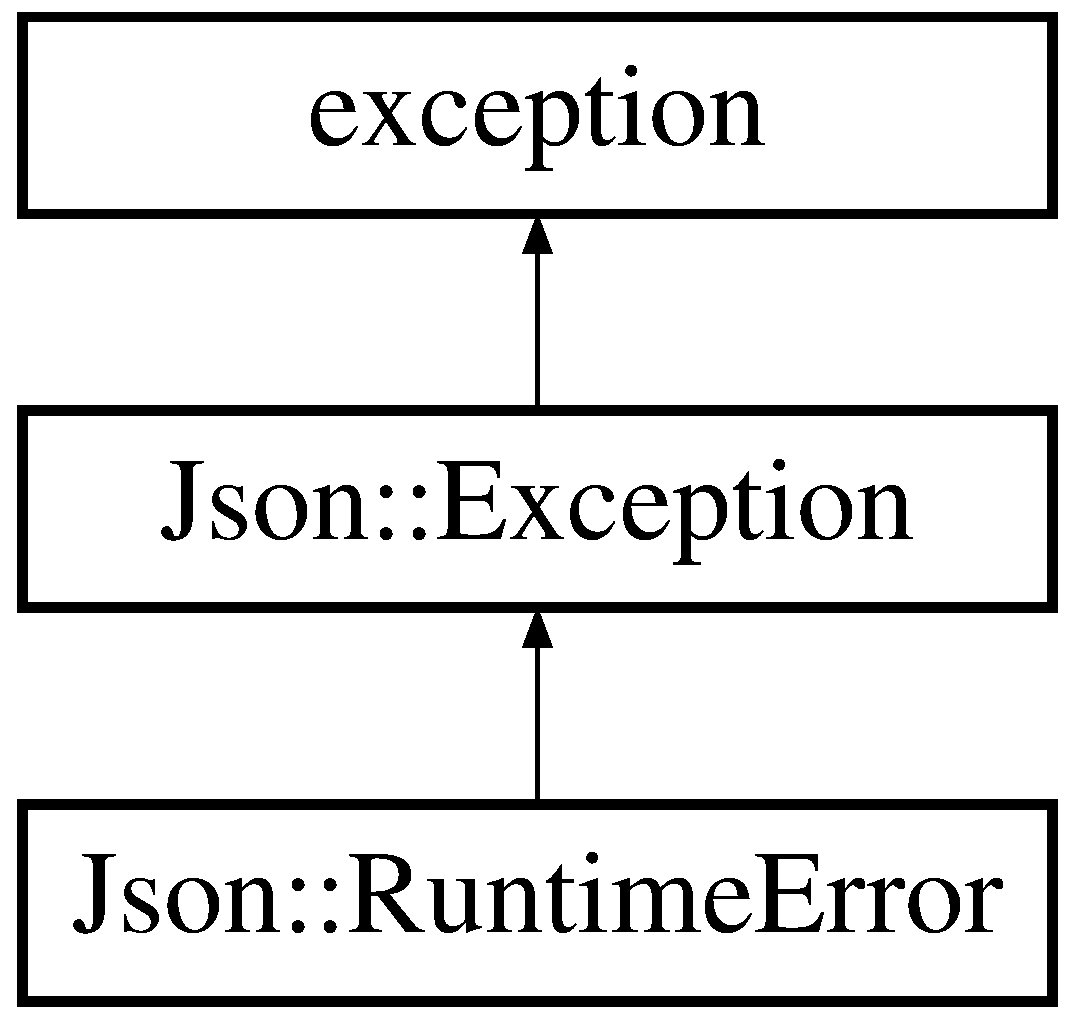
\includegraphics[height=3.000000cm]{classJson_1_1RuntimeError}
\end{center}
\end{figure}
\subsection*{Public Member Functions}
\begin{DoxyCompactItemize}
\item 
\hyperlink{classJson_1_1RuntimeError_a0f6445dc345ce0a703610b6e893fee40_a0f6445dc345ce0a703610b6e893fee40}{Runtime\+Error} (\hyperlink{json_8h_a1e723f95759de062585bc4a8fd3fa4be_a1e723f95759de062585bc4a8fd3fa4be}{J\+S\+O\+N\+C\+P\+P\+\_\+\+S\+T\+R\+I\+NG} const \&msg)
\end{DoxyCompactItemize}
\subsection*{Additional Inherited Members}


\subsection{Detailed Description}
Exceptions which the user cannot easily avoid.

E.\+g. out-\/of-\/memory (when we use malloc), stack-\/overflow, malicious input

\begin{DoxyRemark}{Remarks}
derived from \hyperlink{classJson_1_1Exception}{Json\+::\+Exception} 
\end{DoxyRemark}


\subsection{Constructor \& Destructor Documentation}
\mbox{\Hypertarget{classJson_1_1RuntimeError_a0f6445dc345ce0a703610b6e893fee40_a0f6445dc345ce0a703610b6e893fee40}\label{classJson_1_1RuntimeError_a0f6445dc345ce0a703610b6e893fee40_a0f6445dc345ce0a703610b6e893fee40}} 
\index{Json\+::\+Runtime\+Error@{Json\+::\+Runtime\+Error}!Runtime\+Error@{Runtime\+Error}}
\index{Runtime\+Error@{Runtime\+Error}!Json\+::\+Runtime\+Error@{Json\+::\+Runtime\+Error}}
\subsubsection{\texorpdfstring{Runtime\+Error()}{RuntimeError()}}
{\footnotesize\ttfamily Json\+::\+Runtime\+Error\+::\+Runtime\+Error (\begin{DoxyParamCaption}\item[{\hyperlink{json_8h_a1e723f95759de062585bc4a8fd3fa4be_a1e723f95759de062585bc4a8fd3fa4be}{J\+S\+O\+N\+C\+P\+P\+\_\+\+S\+T\+R\+I\+NG} const \&}]{msg }\end{DoxyParamCaption})}



The documentation for this class was generated from the following files\+:\begin{DoxyCompactItemize}
\item 
json/\hyperlink{json_8h}{json.\+h}\item 
\hyperlink{jsoncpp_8cpp}{jsoncpp.\+cpp}\end{DoxyCompactItemize}

\hypertarget{unionsocket__address}{}\section{socket\+\_\+address Union Reference}
\label{unionsocket__address}\index{socket\+\_\+address@{socket\+\_\+address}}
\subsection*{Public Attributes}
\begin{DoxyCompactItemize}
\item 
\mbox{\Hypertarget{unionsocket__address_ab6a9b0bc545e839df7e06e5b6bff0891}\label{unionsocket__address_ab6a9b0bc545e839df7e06e5b6bff0891}} 
struct sockaddr {\bfseries sa}
\item 
\mbox{\Hypertarget{unionsocket__address_af540a7224ea459c48bc6ec1ca592e55d}\label{unionsocket__address_af540a7224ea459c48bc6ec1ca592e55d}} 
struct sockaddr\+\_\+in {\bfseries sin}
\item 
\mbox{\Hypertarget{unionsocket__address_a923a2caba3cad046553b3632f7c2c571}\label{unionsocket__address_a923a2caba3cad046553b3632f7c2c571}} 
struct sockaddr {\bfseries sin6}
\end{DoxyCompactItemize}


The documentation for this union was generated from the following file\+:\begin{DoxyCompactItemize}
\item 
mongoose.\+h\end{DoxyCompactItemize}

\hypertarget{classJson_1_1StaticString}{}\section{Json\+:\+:Static\+String Class Reference}
\label{classJson_1_1StaticString}\index{Json\+::\+Static\+String@{Json\+::\+Static\+String}}


Lightweight wrapper to tag static string.  




{\ttfamily \#include $<$json.\+h$>$}

\subsection*{Public Member Functions}
\begin{DoxyCompactItemize}
\item 
\hyperlink{classJson_1_1StaticString_afb6baf1ec078ce76f0b0f9b39d19437f_afb6baf1ec078ce76f0b0f9b39d19437f}{Static\+String} (const char $\ast$czstring)
\item 
\hyperlink{classJson_1_1StaticString_a256a6cc0c630aef670848a0f11707b62_a256a6cc0c630aef670848a0f11707b62}{operator const char $\ast$} () const
\item 
const char $\ast$ \hyperlink{classJson_1_1StaticString_ad6be703d432d108623bb0aa06b0b90ca_ad6be703d432d108623bb0aa06b0b90ca}{c\+\_\+str} () const
\end{DoxyCompactItemize}
\subsection*{Private Attributes}
\begin{DoxyCompactItemize}
\item 
const char $\ast$ \hyperlink{classJson_1_1StaticString_a9f0d9e8caee8f8db14e2c8c24760dffd_a9f0d9e8caee8f8db14e2c8c24760dffd}{c\+\_\+str\+\_\+}
\end{DoxyCompactItemize}


\subsection{Detailed Description}
Lightweight wrapper to tag static string. 

\hyperlink{classJson_1_1Value}{Value} constructor and object\+Value member assignement takes advantage of the \hyperlink{classJson_1_1StaticString}{Static\+String} and avoid the cost of string duplication when storing the string or the member name.

Example of usage\+: 
\begin{DoxyCode}
\hyperlink{classJson_1_1Value}{Json::Value} aValue( \hyperlink{classJson_1_1StaticString_afb6baf1ec078ce76f0b0f9b39d19437f_afb6baf1ec078ce76f0b0f9b39d19437f}{StaticString}(\textcolor{stringliteral}{"some text"}) );
\hyperlink{classJson_1_1Value}{Json::Value} object;
\textcolor{keyword}{static} \textcolor{keyword}{const} \hyperlink{classJson_1_1StaticString_afb6baf1ec078ce76f0b0f9b39d19437f_afb6baf1ec078ce76f0b0f9b39d19437f}{StaticString} code(\textcolor{stringliteral}{"code"});
\textcolor{keywordtype}{object}[code] = 1234;
\end{DoxyCode}
 

\subsection{Constructor \& Destructor Documentation}
\mbox{\Hypertarget{classJson_1_1StaticString_afb6baf1ec078ce76f0b0f9b39d19437f_afb6baf1ec078ce76f0b0f9b39d19437f}\label{classJson_1_1StaticString_afb6baf1ec078ce76f0b0f9b39d19437f_afb6baf1ec078ce76f0b0f9b39d19437f}} 
\index{Json\+::\+Static\+String@{Json\+::\+Static\+String}!Static\+String@{Static\+String}}
\index{Static\+String@{Static\+String}!Json\+::\+Static\+String@{Json\+::\+Static\+String}}
\subsubsection{\texorpdfstring{Static\+String()}{StaticString()}}
{\footnotesize\ttfamily Json\+::\+Static\+String\+::\+Static\+String (\begin{DoxyParamCaption}\item[{const char $\ast$}]{czstring }\end{DoxyParamCaption})\hspace{0.3cm}{\ttfamily [inline]}, {\ttfamily [explicit]}}



\subsection{Member Function Documentation}
\mbox{\Hypertarget{classJson_1_1StaticString_ad6be703d432d108623bb0aa06b0b90ca_ad6be703d432d108623bb0aa06b0b90ca}\label{classJson_1_1StaticString_ad6be703d432d108623bb0aa06b0b90ca_ad6be703d432d108623bb0aa06b0b90ca}} 
\index{Json\+::\+Static\+String@{Json\+::\+Static\+String}!c\+\_\+str@{c\+\_\+str}}
\index{c\+\_\+str@{c\+\_\+str}!Json\+::\+Static\+String@{Json\+::\+Static\+String}}
\subsubsection{\texorpdfstring{c\+\_\+str()}{c\_str()}}
{\footnotesize\ttfamily const char$\ast$ Json\+::\+Static\+String\+::c\+\_\+str (\begin{DoxyParamCaption}{ }\end{DoxyParamCaption}) const\hspace{0.3cm}{\ttfamily [inline]}}



Referenced by Json\+::\+Value\+::operator\mbox{[}$\,$\mbox{]}(), and Json\+::\+Value\+::\+Value().

\mbox{\Hypertarget{classJson_1_1StaticString_a256a6cc0c630aef670848a0f11707b62_a256a6cc0c630aef670848a0f11707b62}\label{classJson_1_1StaticString_a256a6cc0c630aef670848a0f11707b62_a256a6cc0c630aef670848a0f11707b62}} 
\index{Json\+::\+Static\+String@{Json\+::\+Static\+String}!operator const char $\ast$@{operator const char $\ast$}}
\index{operator const char $\ast$@{operator const char $\ast$}!Json\+::\+Static\+String@{Json\+::\+Static\+String}}
\subsubsection{\texorpdfstring{operator const char $\ast$()}{operator const char *()}}
{\footnotesize\ttfamily Json\+::\+Static\+String\+::operator const char $\ast$ (\begin{DoxyParamCaption}{ }\end{DoxyParamCaption}) const\hspace{0.3cm}{\ttfamily [inline]}}



\subsection{Member Data Documentation}
\mbox{\Hypertarget{classJson_1_1StaticString_a9f0d9e8caee8f8db14e2c8c24760dffd_a9f0d9e8caee8f8db14e2c8c24760dffd}\label{classJson_1_1StaticString_a9f0d9e8caee8f8db14e2c8c24760dffd_a9f0d9e8caee8f8db14e2c8c24760dffd}} 
\index{Json\+::\+Static\+String@{Json\+::\+Static\+String}!c\+\_\+str\+\_\+@{c\+\_\+str\+\_\+}}
\index{c\+\_\+str\+\_\+@{c\+\_\+str\+\_\+}!Json\+::\+Static\+String@{Json\+::\+Static\+String}}
\subsubsection{\texorpdfstring{c\+\_\+str\+\_\+}{c\_str\_}}
{\footnotesize\ttfamily const char$\ast$ Json\+::\+Static\+String\+::c\+\_\+str\+\_\+\hspace{0.3cm}{\ttfamily [private]}}



The documentation for this class was generated from the following file\+:\begin{DoxyCompactItemize}
\item 
json/\hyperlink{json_8h}{json.\+h}\end{DoxyCompactItemize}

\hypertarget{classJson_1_1StreamWriter}{}\section{Json\+:\+:Stream\+Writer Class Reference}
\label{classJson_1_1StreamWriter}\index{Json\+::\+Stream\+Writer@{Json\+::\+Stream\+Writer}}


{\ttfamily \#include $<$json.\+h$>$}

Inheritance diagram for Json\+:\+:Stream\+Writer\+:\begin{figure}[H]
\begin{center}
\leavevmode
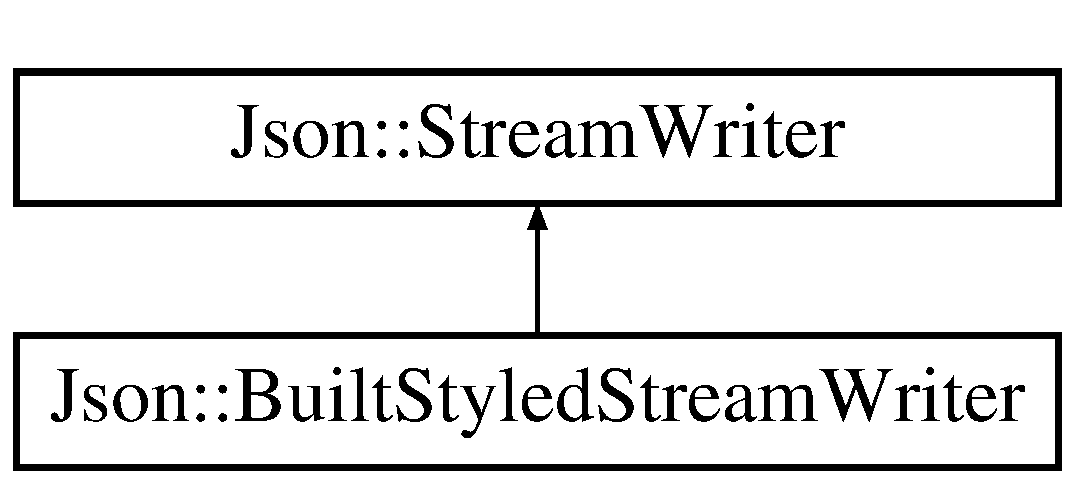
\includegraphics[height=2.000000cm]{classJson_1_1StreamWriter}
\end{center}
\end{figure}
\subsection*{Classes}
\begin{DoxyCompactItemize}
\item 
class \hyperlink{classJson_1_1StreamWriter_1_1Factory}{Factory}
\begin{DoxyCompactList}\small\item\em A simple abstract factory. \end{DoxyCompactList}\end{DoxyCompactItemize}
\subsection*{Public Member Functions}
\begin{DoxyCompactItemize}
\item 
\hyperlink{classJson_1_1StreamWriter_a66e6f5113618ce6b04cac9b3c85a3707_a66e6f5113618ce6b04cac9b3c85a3707}{Stream\+Writer} ()
\item 
virtual \hyperlink{classJson_1_1StreamWriter_a03f8fb6a873b6b50f05bc4556e043c3a_a03f8fb6a873b6b50f05bc4556e043c3a}{$\sim$\+Stream\+Writer} ()
\item 
virtual int \hyperlink{classJson_1_1StreamWriter_a84278bad0c9a9fc587bc2a97c5bb5993_a84278bad0c9a9fc587bc2a97c5bb5993}{write} (\hyperlink{classJson_1_1Value}{Value} const \&root, \hyperlink{json_8h_a37a25be5fca174927780caeb280094ce_a37a25be5fca174927780caeb280094ce}{J\+S\+O\+N\+C\+P\+P\+\_\+\+O\+S\+T\+R\+E\+AM} $\ast$sout)=0
\end{DoxyCompactItemize}
\subsection*{Protected Attributes}
\begin{DoxyCompactItemize}
\item 
\hyperlink{json_8h_a37a25be5fca174927780caeb280094ce_a37a25be5fca174927780caeb280094ce}{J\+S\+O\+N\+C\+P\+P\+\_\+\+O\+S\+T\+R\+E\+AM} $\ast$ \hyperlink{classJson_1_1StreamWriter_a4f5603d4228a9fa46a42cb44e5234d9b_a4f5603d4228a9fa46a42cb44e5234d9b}{sout\+\_\+}
\end{DoxyCompactItemize}


\subsection{Detailed Description}
Usage\+: 
\begin{DoxyCode}
\textcolor{keyword}{using namespace }\hyperlink{namespaceJson}{Json};
\textcolor{keywordtype}{void} writeToStdout(\hyperlink{classJson_1_1StreamWriter_1_1Factory}{StreamWriter::Factory} \textcolor{keyword}{const}& factory, 
      \hyperlink{classJson_1_1Value}{Value} \textcolor{keyword}{const}& value) \{
  std::unique\_ptr<StreamWriter> \textcolor{keyword}{const} writer(
    factory.\hyperlink{classJson_1_1StreamWriter_1_1Factory_a9d30ec53e8288cd53befccf1009c5f31_a9d30ec53e8288cd53befccf1009c5f31}{newStreamWriter}());
  writer->write(value, &std::cout);
  std::cout << std::endl;  \textcolor{comment}{// add lf and flush}
\}
\end{DoxyCode}
 

\subsection{Constructor \& Destructor Documentation}
\mbox{\Hypertarget{classJson_1_1StreamWriter_a66e6f5113618ce6b04cac9b3c85a3707_a66e6f5113618ce6b04cac9b3c85a3707}\label{classJson_1_1StreamWriter_a66e6f5113618ce6b04cac9b3c85a3707_a66e6f5113618ce6b04cac9b3c85a3707}} 
\index{Json\+::\+Stream\+Writer@{Json\+::\+Stream\+Writer}!Stream\+Writer@{Stream\+Writer}}
\index{Stream\+Writer@{Stream\+Writer}!Json\+::\+Stream\+Writer@{Json\+::\+Stream\+Writer}}
\subsubsection{\texorpdfstring{Stream\+Writer()}{StreamWriter()}}
{\footnotesize\ttfamily Json\+::\+Stream\+Writer\+::\+Stream\+Writer (\begin{DoxyParamCaption}{ }\end{DoxyParamCaption})}

\mbox{\Hypertarget{classJson_1_1StreamWriter_a03f8fb6a873b6b50f05bc4556e043c3a_a03f8fb6a873b6b50f05bc4556e043c3a}\label{classJson_1_1StreamWriter_a03f8fb6a873b6b50f05bc4556e043c3a_a03f8fb6a873b6b50f05bc4556e043c3a}} 
\index{Json\+::\+Stream\+Writer@{Json\+::\+Stream\+Writer}!````~Stream\+Writer@{$\sim$\+Stream\+Writer}}
\index{````~Stream\+Writer@{$\sim$\+Stream\+Writer}!Json\+::\+Stream\+Writer@{Json\+::\+Stream\+Writer}}
\subsubsection{\texorpdfstring{$\sim$\+Stream\+Writer()}{~StreamWriter()}}
{\footnotesize\ttfamily Json\+::\+Stream\+Writer\+::$\sim$\+Stream\+Writer (\begin{DoxyParamCaption}{ }\end{DoxyParamCaption})\hspace{0.3cm}{\ttfamily [virtual]}}



\subsection{Member Function Documentation}
\mbox{\Hypertarget{classJson_1_1StreamWriter_a84278bad0c9a9fc587bc2a97c5bb5993_a84278bad0c9a9fc587bc2a97c5bb5993}\label{classJson_1_1StreamWriter_a84278bad0c9a9fc587bc2a97c5bb5993_a84278bad0c9a9fc587bc2a97c5bb5993}} 
\index{Json\+::\+Stream\+Writer@{Json\+::\+Stream\+Writer}!write@{write}}
\index{write@{write}!Json\+::\+Stream\+Writer@{Json\+::\+Stream\+Writer}}
\subsubsection{\texorpdfstring{write()}{write()}}
{\footnotesize\ttfamily virtual int Json\+::\+Stream\+Writer\+::write (\begin{DoxyParamCaption}\item[{\hyperlink{classJson_1_1Value}{Value} const \&}]{root,  }\item[{\hyperlink{json_8h_a37a25be5fca174927780caeb280094ce_a37a25be5fca174927780caeb280094ce}{J\+S\+O\+N\+C\+P\+P\+\_\+\+O\+S\+T\+R\+E\+AM} $\ast$}]{sout }\end{DoxyParamCaption})\hspace{0.3cm}{\ttfamily [pure virtual]}}

Write \hyperlink{classJson_1_1Value}{Value} into document as configured in sub-\/class. Do not take ownership of sout, but maintain a reference during function. \begin{DoxyPrecond}{Precondition}
sout != N\+U\+LL 
\end{DoxyPrecond}
\begin{DoxyReturn}{Returns}
zero on success (For now, we always return zero, so check the stream instead.) 
\end{DoxyReturn}

\begin{DoxyExceptions}{Exceptions}
{\em std\+::exception} & possibly, depending on configuration \\
\hline
\end{DoxyExceptions}


Implemented in \hyperlink{structJson_1_1BuiltStyledStreamWriter_a823cdb1afabb6b0d5f39bcd5a6a6f747_a823cdb1afabb6b0d5f39bcd5a6a6f747}{Json\+::\+Built\+Styled\+Stream\+Writer}.



\subsection{Member Data Documentation}
\mbox{\Hypertarget{classJson_1_1StreamWriter_a4f5603d4228a9fa46a42cb44e5234d9b_a4f5603d4228a9fa46a42cb44e5234d9b}\label{classJson_1_1StreamWriter_a4f5603d4228a9fa46a42cb44e5234d9b_a4f5603d4228a9fa46a42cb44e5234d9b}} 
\index{Json\+::\+Stream\+Writer@{Json\+::\+Stream\+Writer}!sout\+\_\+@{sout\+\_\+}}
\index{sout\+\_\+@{sout\+\_\+}!Json\+::\+Stream\+Writer@{Json\+::\+Stream\+Writer}}
\subsubsection{\texorpdfstring{sout\+\_\+}{sout\_}}
{\footnotesize\ttfamily \hyperlink{json_8h_a37a25be5fca174927780caeb280094ce_a37a25be5fca174927780caeb280094ce}{J\+S\+O\+N\+C\+P\+P\+\_\+\+O\+S\+T\+R\+E\+AM}$\ast$ Json\+::\+Stream\+Writer\+::sout\+\_\+\hspace{0.3cm}{\ttfamily [protected]}}



Referenced by Json\+::\+Built\+Styled\+Stream\+Writer\+::push\+Value(), Json\+::\+Built\+Styled\+Stream\+Writer\+::write(), Json\+::\+Built\+Styled\+Stream\+Writer\+::write\+Array\+Value(), Json\+::\+Built\+Styled\+Stream\+Writer\+::write\+Comment\+After\+Value\+On\+Same\+Line(), Json\+::\+Built\+Styled\+Stream\+Writer\+::write\+Comment\+Before\+Value(), Json\+::\+Built\+Styled\+Stream\+Writer\+::write\+Indent(), Json\+::\+Built\+Styled\+Stream\+Writer\+::write\+Value(), and Json\+::\+Built\+Styled\+Stream\+Writer\+::write\+With\+Indent().



The documentation for this class was generated from the following files\+:\begin{DoxyCompactItemize}
\item 
json/\hyperlink{json_8h}{json.\+h}\item 
\hyperlink{jsoncpp_8cpp}{jsoncpp.\+cpp}\end{DoxyCompactItemize}

\hypertarget{classJson_1_1StreamWriterBuilder}{}\section{Json\+:\+:Stream\+Writer\+Builder Class Reference}
\label{classJson_1_1StreamWriterBuilder}\index{Json\+::\+Stream\+Writer\+Builder@{Json\+::\+Stream\+Writer\+Builder}}


Build a \hyperlink{classJson_1_1StreamWriter}{Stream\+Writer} implementation.  




{\ttfamily \#include $<$json.\+h$>$}

Inheritance diagram for Json\+:\+:Stream\+Writer\+Builder\+:\begin{figure}[H]
\begin{center}
\leavevmode
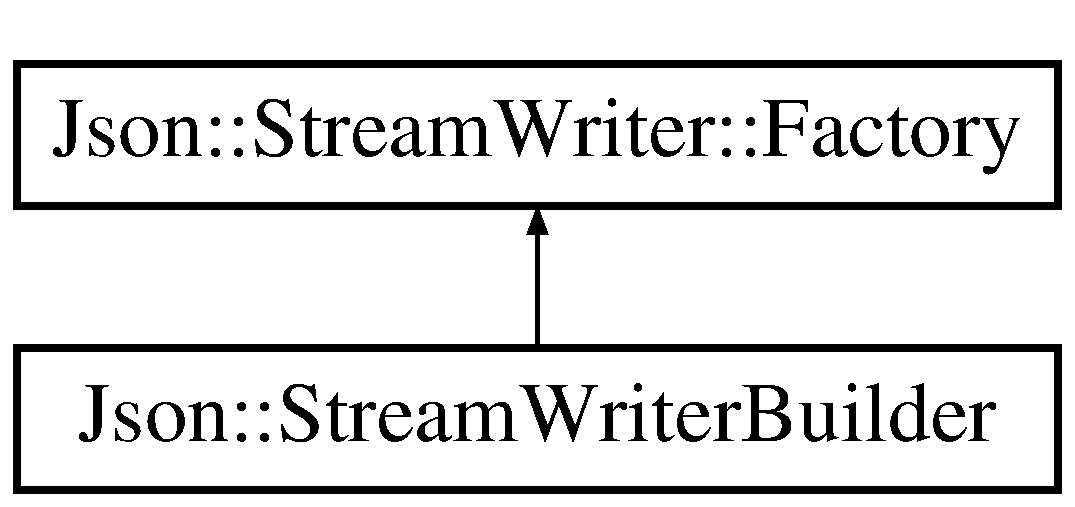
\includegraphics[height=2.000000cm]{classJson_1_1StreamWriterBuilder}
\end{center}
\end{figure}
\subsection*{Public Member Functions}
\begin{DoxyCompactItemize}
\item 
\hyperlink{classJson_1_1StreamWriterBuilder_ab95b76179c152673ad14abc639a46ee4_ab95b76179c152673ad14abc639a46ee4}{Stream\+Writer\+Builder} ()
\item 
\hyperlink{classJson_1_1StreamWriterBuilder_a93263f8ef1e2d22593907075d8f0aaef_a93263f8ef1e2d22593907075d8f0aaef}{$\sim$\+Stream\+Writer\+Builder} () \hyperlink{json_8h_a824d6199c91488107e443226fa6022c5_a824d6199c91488107e443226fa6022c5}{J\+S\+O\+N\+C\+P\+P\+\_\+\+O\+V\+E\+R\+R\+I\+DE}
\item 
\hyperlink{classJson_1_1StreamWriter}{Stream\+Writer} $\ast$ \hyperlink{classJson_1_1StreamWriterBuilder_ab9ee278609f88ae04a7c1a84e1f559e6_ab9ee278609f88ae04a7c1a84e1f559e6}{new\+Stream\+Writer} () const \hyperlink{json_8h_a824d6199c91488107e443226fa6022c5_a824d6199c91488107e443226fa6022c5}{J\+S\+O\+N\+C\+P\+P\+\_\+\+O\+V\+E\+R\+R\+I\+DE}
\item 
bool \hyperlink{classJson_1_1StreamWriterBuilder_a12353b97766841db7d049da84658da09_a12353b97766841db7d049da84658da09}{validate} (\hyperlink{classJson_1_1Value}{Json\+::\+Value} $\ast$invalid) const
\item 
\hyperlink{classJson_1_1Value}{Value} \& \hyperlink{classJson_1_1StreamWriterBuilder_af68f6b59cb20b074052ed12bb3d336a3_af68f6b59cb20b074052ed12bb3d336a3}{operator\mbox{[}$\,$\mbox{]}} (\hyperlink{json_8h_a1e723f95759de062585bc4a8fd3fa4be_a1e723f95759de062585bc4a8fd3fa4be}{J\+S\+O\+N\+C\+P\+P\+\_\+\+S\+T\+R\+I\+NG} key)
\end{DoxyCompactItemize}
\subsection*{Static Public Member Functions}
\begin{DoxyCompactItemize}
\item 
static void \hyperlink{classJson_1_1StreamWriterBuilder_a53bf106b141e28637b01ad0ecd2acbf6_a53bf106b141e28637b01ad0ecd2acbf6}{set\+Defaults} (\hyperlink{classJson_1_1Value}{Json\+::\+Value} $\ast$settings)
\end{DoxyCompactItemize}
\subsection*{Public Attributes}
\begin{DoxyCompactItemize}
\item 
\hyperlink{classJson_1_1Value}{Json\+::\+Value} \hyperlink{classJson_1_1StreamWriterBuilder_a79bdf2e639a52f4e758c0b95bd1d3423_a79bdf2e639a52f4e758c0b95bd1d3423}{settings\+\_\+}
\end{DoxyCompactItemize}


\subsection{Detailed Description}
Build a \hyperlink{classJson_1_1StreamWriter}{Stream\+Writer} implementation. 

Usage\+: 
\begin{DoxyCode}
\textcolor{keyword}{using namespace }\hyperlink{namespaceJson}{Json};
\hyperlink{classJson_1_1Value}{Value} value = ...;
\hyperlink{classJson_1_1StreamWriterBuilder}{StreamWriterBuilder} builder;
builder[\textcolor{stringliteral}{"commentStyle"}] = \textcolor{stringliteral}{"None"};
builder[\textcolor{stringliteral}{"indentation"}] = \textcolor{stringliteral}{"   "};  \textcolor{comment}{// or whatever you like}
std::unique\_ptr<Json::StreamWriter> writer(
    builder.\hyperlink{classJson_1_1StreamWriterBuilder_ab9ee278609f88ae04a7c1a84e1f559e6_ab9ee278609f88ae04a7c1a84e1f559e6}{newStreamWriter}());
writer->write(value, &std::cout);
std::cout << std::endl;  \textcolor{comment}{// add lf and flush}
\end{DoxyCode}
 

\subsection{Constructor \& Destructor Documentation}
\mbox{\Hypertarget{classJson_1_1StreamWriterBuilder_ab95b76179c152673ad14abc639a46ee4_ab95b76179c152673ad14abc639a46ee4}\label{classJson_1_1StreamWriterBuilder_ab95b76179c152673ad14abc639a46ee4_ab95b76179c152673ad14abc639a46ee4}} 
\index{Json\+::\+Stream\+Writer\+Builder@{Json\+::\+Stream\+Writer\+Builder}!Stream\+Writer\+Builder@{Stream\+Writer\+Builder}}
\index{Stream\+Writer\+Builder@{Stream\+Writer\+Builder}!Json\+::\+Stream\+Writer\+Builder@{Json\+::\+Stream\+Writer\+Builder}}
\subsubsection{\texorpdfstring{Stream\+Writer\+Builder()}{StreamWriterBuilder()}}
{\footnotesize\ttfamily Json\+::\+Stream\+Writer\+Builder\+::\+Stream\+Writer\+Builder (\begin{DoxyParamCaption}{ }\end{DoxyParamCaption})}

\mbox{\Hypertarget{classJson_1_1StreamWriterBuilder_a93263f8ef1e2d22593907075d8f0aaef_a93263f8ef1e2d22593907075d8f0aaef}\label{classJson_1_1StreamWriterBuilder_a93263f8ef1e2d22593907075d8f0aaef_a93263f8ef1e2d22593907075d8f0aaef}} 
\index{Json\+::\+Stream\+Writer\+Builder@{Json\+::\+Stream\+Writer\+Builder}!````~Stream\+Writer\+Builder@{$\sim$\+Stream\+Writer\+Builder}}
\index{````~Stream\+Writer\+Builder@{$\sim$\+Stream\+Writer\+Builder}!Json\+::\+Stream\+Writer\+Builder@{Json\+::\+Stream\+Writer\+Builder}}
\subsubsection{\texorpdfstring{$\sim$\+Stream\+Writer\+Builder()}{~StreamWriterBuilder()}}
{\footnotesize\ttfamily Json\+::\+Stream\+Writer\+Builder\+::$\sim$\+Stream\+Writer\+Builder (\begin{DoxyParamCaption}{ }\end{DoxyParamCaption})}



\subsection{Member Function Documentation}
\mbox{\Hypertarget{classJson_1_1StreamWriterBuilder_ab9ee278609f88ae04a7c1a84e1f559e6_ab9ee278609f88ae04a7c1a84e1f559e6}\label{classJson_1_1StreamWriterBuilder_ab9ee278609f88ae04a7c1a84e1f559e6_ab9ee278609f88ae04a7c1a84e1f559e6}} 
\index{Json\+::\+Stream\+Writer\+Builder@{Json\+::\+Stream\+Writer\+Builder}!new\+Stream\+Writer@{new\+Stream\+Writer}}
\index{new\+Stream\+Writer@{new\+Stream\+Writer}!Json\+::\+Stream\+Writer\+Builder@{Json\+::\+Stream\+Writer\+Builder}}
\subsubsection{\texorpdfstring{new\+Stream\+Writer()}{newStreamWriter()}}
{\footnotesize\ttfamily \hyperlink{classJson_1_1StreamWriter}{Stream\+Writer} $\ast$ Json\+::\+Stream\+Writer\+Builder\+::new\+Stream\+Writer (\begin{DoxyParamCaption}{ }\end{DoxyParamCaption}) const\hspace{0.3cm}{\ttfamily [virtual]}}


\begin{DoxyExceptions}{Exceptions}
{\em std\+::exception} & if something goes wrong (e.\+g. invalid settings) \\
\hline
\end{DoxyExceptions}


Implements \hyperlink{classJson_1_1StreamWriter_1_1Factory_a9d30ec53e8288cd53befccf1009c5f31_a9d30ec53e8288cd53befccf1009c5f31}{Json\+::\+Stream\+Writer\+::\+Factory}.



References Json\+::\+Comment\+Style\+::\+All, J\+S\+O\+N\+C\+P\+P\+\_\+\+S\+T\+R\+I\+NG, Json\+::\+Comment\+Style\+::\+None, and Json\+::throw\+Runtime\+Error().



Referenced by Json\+::operator$<$$<$().

\mbox{\Hypertarget{classJson_1_1StreamWriterBuilder_af68f6b59cb20b074052ed12bb3d336a3_af68f6b59cb20b074052ed12bb3d336a3}\label{classJson_1_1StreamWriterBuilder_af68f6b59cb20b074052ed12bb3d336a3_af68f6b59cb20b074052ed12bb3d336a3}} 
\index{Json\+::\+Stream\+Writer\+Builder@{Json\+::\+Stream\+Writer\+Builder}!operator\mbox{[}\mbox{]}@{operator[]}}
\index{operator\mbox{[}\mbox{]}@{operator[]}!Json\+::\+Stream\+Writer\+Builder@{Json\+::\+Stream\+Writer\+Builder}}
\subsubsection{\texorpdfstring{operator[]()}{operator[]()}}
{\footnotesize\ttfamily \hyperlink{classJson_1_1Value}{Value} \& Json\+::\+Stream\+Writer\+Builder\+::operator\mbox{[}$\,$\mbox{]} (\begin{DoxyParamCaption}\item[{\hyperlink{json_8h_a1e723f95759de062585bc4a8fd3fa4be_a1e723f95759de062585bc4a8fd3fa4be}{J\+S\+O\+N\+C\+P\+P\+\_\+\+S\+T\+R\+I\+NG}}]{key }\end{DoxyParamCaption})}

A simple way to update a specific setting. \mbox{\Hypertarget{classJson_1_1StreamWriterBuilder_a53bf106b141e28637b01ad0ecd2acbf6_a53bf106b141e28637b01ad0ecd2acbf6}\label{classJson_1_1StreamWriterBuilder_a53bf106b141e28637b01ad0ecd2acbf6_a53bf106b141e28637b01ad0ecd2acbf6}} 
\index{Json\+::\+Stream\+Writer\+Builder@{Json\+::\+Stream\+Writer\+Builder}!set\+Defaults@{set\+Defaults}}
\index{set\+Defaults@{set\+Defaults}!Json\+::\+Stream\+Writer\+Builder@{Json\+::\+Stream\+Writer\+Builder}}
\subsubsection{\texorpdfstring{set\+Defaults()}{setDefaults()}}
{\footnotesize\ttfamily void Json\+::\+Stream\+Writer\+Builder\+::set\+Defaults (\begin{DoxyParamCaption}\item[{\hyperlink{classJson_1_1Value}{Json\+::\+Value} $\ast$}]{settings }\end{DoxyParamCaption})\hspace{0.3cm}{\ttfamily [static]}}

Called by ctor, but you can use this to reset settings\+\_\+. \begin{DoxyPrecond}{Precondition}
\textquotesingle{}settings\textquotesingle{} != N\+U\+LL (but Json\+::null is fine) 
\end{DoxyPrecond}
\begin{DoxyRemark}{Remarks}
Defaults\+: 
\begin{DoxyCodeInclude}
\end{DoxyCodeInclude}

\end{DoxyRemark}
\mbox{[}Stream\+Writer\+Builder\+Defaults\mbox{]}

\mbox{[}Stream\+Writer\+Builder\+Defaults\mbox{]} \mbox{\Hypertarget{classJson_1_1StreamWriterBuilder_a12353b97766841db7d049da84658da09_a12353b97766841db7d049da84658da09}\label{classJson_1_1StreamWriterBuilder_a12353b97766841db7d049da84658da09_a12353b97766841db7d049da84658da09}} 
\index{Json\+::\+Stream\+Writer\+Builder@{Json\+::\+Stream\+Writer\+Builder}!validate@{validate}}
\index{validate@{validate}!Json\+::\+Stream\+Writer\+Builder@{Json\+::\+Stream\+Writer\+Builder}}
\subsubsection{\texorpdfstring{validate()}{validate()}}
{\footnotesize\ttfamily bool Json\+::\+Stream\+Writer\+Builder\+::validate (\begin{DoxyParamCaption}\item[{\hyperlink{classJson_1_1Value}{Json\+::\+Value} $\ast$}]{invalid }\end{DoxyParamCaption}) const}

\begin{DoxyReturn}{Returns}
true if \textquotesingle{}settings\textquotesingle{} are legal and consistent; otherwise, indicate bad settings via \textquotesingle{}invalid\textquotesingle{}. 
\end{DoxyReturn}


References Json\+::get\+Valid\+Writer\+Keys(), J\+S\+O\+N\+C\+P\+P\+\_\+\+S\+T\+R\+I\+NG, and Json\+::\+Value\+::size().



\subsection{Member Data Documentation}
\mbox{\Hypertarget{classJson_1_1StreamWriterBuilder_a79bdf2e639a52f4e758c0b95bd1d3423_a79bdf2e639a52f4e758c0b95bd1d3423}\label{classJson_1_1StreamWriterBuilder_a79bdf2e639a52f4e758c0b95bd1d3423_a79bdf2e639a52f4e758c0b95bd1d3423}} 
\index{Json\+::\+Stream\+Writer\+Builder@{Json\+::\+Stream\+Writer\+Builder}!settings\+\_\+@{settings\+\_\+}}
\index{settings\+\_\+@{settings\+\_\+}!Json\+::\+Stream\+Writer\+Builder@{Json\+::\+Stream\+Writer\+Builder}}
\subsubsection{\texorpdfstring{settings\+\_\+}{settings\_}}
{\footnotesize\ttfamily \hyperlink{classJson_1_1Value}{Json\+::\+Value} Json\+::\+Stream\+Writer\+Builder\+::settings\+\_\+}

Configuration of this builder. Available settings (case-\/sensitive)\+:
\begin{DoxyItemize}
\item \char`\"{}comment\+Style\char`\"{}\+: \char`\"{}\+None\char`\"{} or \char`\"{}\+All\char`\"{}
\item \char`\"{}indentation\char`\"{}\+: \char`\"{}$<$anything$>$\char`\"{}
\item \char`\"{}enable\+Y\+A\+M\+L\+Compatibility\char`\"{}\+: false or true
\begin{DoxyItemize}
\item slightly change the whitespace around colons
\end{DoxyItemize}
\item \char`\"{}drop\+Null\+Placeholders\char`\"{}\+: false or true
\begin{DoxyItemize}
\item Drop the \char`\"{}null\char`\"{} string from the writer\textquotesingle{}s output for null\+Values. Strictly speaking, this is not valid J\+S\+ON. But when the output is being fed to a browser\textquotesingle{}s Javascript, it makes for smaller output and the browser can handle the output just fine.
\end{DoxyItemize}
\item \char`\"{}use\+Special\+Floats\char`\"{}\+: false or true
\begin{DoxyItemize}
\item If true, outputs non-\/finite floating point values in the following way\+: NaN values as \char`\"{}\+Na\+N\char`\"{}, positive infinity as \char`\"{}\+Infinity\char`\"{}, and negative infinity as \char`\"{}-\/\+Infinity\char`\"{}.
\end{DoxyItemize}
\end{DoxyItemize}

You can examine \textquotesingle{}settings\+\_\+` yourself to see the defaults. You can also write and read them just like any J\+S\+ON \hyperlink{classJson_1_1Value}{Value}. \begin{DoxySeeAlso}{See also}
\hyperlink{classJson_1_1StreamWriterBuilder_a53bf106b141e28637b01ad0ecd2acbf6_a53bf106b141e28637b01ad0ecd2acbf6}{set\+Defaults()} 
\end{DoxySeeAlso}


The documentation for this class was generated from the following files\+:\begin{DoxyCompactItemize}
\item 
json/\hyperlink{json_8h}{json.\+h}\item 
\hyperlink{jsoncpp_8cpp}{jsoncpp.\+cpp}\end{DoxyCompactItemize}

\hypertarget{structJson_1_1Value_1_1CZString_1_1StringStorage}{}\section{Json\+:\+:Value\+:\+:C\+Z\+String\+:\+:String\+Storage Struct Reference}
\label{structJson_1_1Value_1_1CZString_1_1StringStorage}\index{Json\+::\+Value\+::\+C\+Z\+String\+::\+String\+Storage@{Json\+::\+Value\+::\+C\+Z\+String\+::\+String\+Storage}}
\subsection*{Public Attributes}
\begin{DoxyCompactItemize}
\item 
unsigned \hyperlink{structJson_1_1Value_1_1CZString_1_1StringStorage_a7f68c8d6197c5692a525854b5f29f87b_a7f68c8d6197c5692a525854b5f29f87b}{policy\+\_\+}\+: 2
\item 
unsigned \hyperlink{structJson_1_1Value_1_1CZString_1_1StringStorage_a165d865c44e6471d34668eeb4f15b140_a165d865c44e6471d34668eeb4f15b140}{length\+\_\+}\+: 30
\end{DoxyCompactItemize}


\subsection{Member Data Documentation}
\mbox{\Hypertarget{structJson_1_1Value_1_1CZString_1_1StringStorage_a165d865c44e6471d34668eeb4f15b140_a165d865c44e6471d34668eeb4f15b140}\label{structJson_1_1Value_1_1CZString_1_1StringStorage_a165d865c44e6471d34668eeb4f15b140_a165d865c44e6471d34668eeb4f15b140}} 
\index{Json\+::\+Value\+::\+C\+Z\+String\+::\+String\+Storage@{Json\+::\+Value\+::\+C\+Z\+String\+::\+String\+Storage}!length\+\_\+@{length\+\_\+}}
\index{length\+\_\+@{length\+\_\+}!Json\+::\+Value\+::\+C\+Z\+String\+::\+String\+Storage@{Json\+::\+Value\+::\+C\+Z\+String\+::\+String\+Storage}}
\subsubsection{\texorpdfstring{length\+\_\+}{length\_}}
{\footnotesize\ttfamily unsigned Json\+::\+Value\+::\+C\+Z\+String\+::\+String\+Storage\+::length\+\_\+}



Referenced by Json\+::\+Value\+::\+C\+Z\+String\+::\+C\+Z\+String(), Json\+::\+Value\+::\+C\+Z\+String\+::length(), Json\+::\+Value\+::\+C\+Z\+String\+::operator$<$(), Json\+::\+Value\+::\+C\+Z\+String\+::operator==(), and Json\+::\+Value\+::\+C\+Z\+String\+::$\sim$\+C\+Z\+String().

\mbox{\Hypertarget{structJson_1_1Value_1_1CZString_1_1StringStorage_a7f68c8d6197c5692a525854b5f29f87b_a7f68c8d6197c5692a525854b5f29f87b}\label{structJson_1_1Value_1_1CZString_1_1StringStorage_a7f68c8d6197c5692a525854b5f29f87b_a7f68c8d6197c5692a525854b5f29f87b}} 
\index{Json\+::\+Value\+::\+C\+Z\+String\+::\+String\+Storage@{Json\+::\+Value\+::\+C\+Z\+String\+::\+String\+Storage}!policy\+\_\+@{policy\+\_\+}}
\index{policy\+\_\+@{policy\+\_\+}!Json\+::\+Value\+::\+C\+Z\+String\+::\+String\+Storage@{Json\+::\+Value\+::\+C\+Z\+String\+::\+String\+Storage}}
\subsubsection{\texorpdfstring{policy\+\_\+}{policy\_}}
{\footnotesize\ttfamily unsigned Json\+::\+Value\+::\+C\+Z\+String\+::\+String\+Storage\+::policy\+\_\+}



Referenced by Json\+::\+Value\+::\+C\+Z\+String\+::\+C\+Z\+String(), Json\+::\+Value\+::\+C\+Z\+String\+::is\+Static\+String(), and Json\+::\+Value\+::\+C\+Z\+String\+::$\sim$\+C\+Z\+String().



The documentation for this struct was generated from the following file\+:\begin{DoxyCompactItemize}
\item 
json/\hyperlink{json_8h}{json.\+h}\end{DoxyCompactItemize}

\hypertarget{structJson_1_1OurReader_1_1StructuredError}{}\section{Json\+:\+:Our\+Reader\+:\+:Structured\+Error Struct Reference}
\label{structJson_1_1OurReader_1_1StructuredError}\index{Json\+::\+Our\+Reader\+::\+Structured\+Error@{Json\+::\+Our\+Reader\+::\+Structured\+Error}}
\subsection*{Public Attributes}
\begin{DoxyCompactItemize}
\item 
ptrdiff\+\_\+t \hyperlink{structJson_1_1OurReader_1_1StructuredError_a102677698afb8177c985e72dafe72b15_a102677698afb8177c985e72dafe72b15}{offset\+\_\+start}
\item 
ptrdiff\+\_\+t \hyperlink{structJson_1_1OurReader_1_1StructuredError_a15491a751a39c5153af04e68b1d0abb9_a15491a751a39c5153af04e68b1d0abb9}{offset\+\_\+limit}
\item 
\hyperlink{json_8h_a1e723f95759de062585bc4a8fd3fa4be_a1e723f95759de062585bc4a8fd3fa4be}{J\+S\+O\+N\+C\+P\+P\+\_\+\+S\+T\+R\+I\+NG} \hyperlink{structJson_1_1OurReader_1_1StructuredError_a9d0b9986bf765d067dfcf2f971a450d1_a9d0b9986bf765d067dfcf2f971a450d1}{message}
\end{DoxyCompactItemize}


\subsection{Member Data Documentation}
\mbox{\Hypertarget{structJson_1_1OurReader_1_1StructuredError_a9d0b9986bf765d067dfcf2f971a450d1_a9d0b9986bf765d067dfcf2f971a450d1}\label{structJson_1_1OurReader_1_1StructuredError_a9d0b9986bf765d067dfcf2f971a450d1_a9d0b9986bf765d067dfcf2f971a450d1}} 
\index{Json\+::\+Our\+Reader\+::\+Structured\+Error@{Json\+::\+Our\+Reader\+::\+Structured\+Error}!message@{message}}
\index{message@{message}!Json\+::\+Our\+Reader\+::\+Structured\+Error@{Json\+::\+Our\+Reader\+::\+Structured\+Error}}
\subsubsection{\texorpdfstring{message}{message}}
{\footnotesize\ttfamily \hyperlink{json_8h_a1e723f95759de062585bc4a8fd3fa4be_a1e723f95759de062585bc4a8fd3fa4be}{J\+S\+O\+N\+C\+P\+P\+\_\+\+S\+T\+R\+I\+NG} Json\+::\+Our\+Reader\+::\+Structured\+Error\+::message}



Referenced by Json\+::\+Our\+Reader\+::get\+Structured\+Errors().

\mbox{\Hypertarget{structJson_1_1OurReader_1_1StructuredError_a15491a751a39c5153af04e68b1d0abb9_a15491a751a39c5153af04e68b1d0abb9}\label{structJson_1_1OurReader_1_1StructuredError_a15491a751a39c5153af04e68b1d0abb9_a15491a751a39c5153af04e68b1d0abb9}} 
\index{Json\+::\+Our\+Reader\+::\+Structured\+Error@{Json\+::\+Our\+Reader\+::\+Structured\+Error}!offset\+\_\+limit@{offset\+\_\+limit}}
\index{offset\+\_\+limit@{offset\+\_\+limit}!Json\+::\+Our\+Reader\+::\+Structured\+Error@{Json\+::\+Our\+Reader\+::\+Structured\+Error}}
\subsubsection{\texorpdfstring{offset\+\_\+limit}{offset\_limit}}
{\footnotesize\ttfamily ptrdiff\+\_\+t Json\+::\+Our\+Reader\+::\+Structured\+Error\+::offset\+\_\+limit}



Referenced by Json\+::\+Our\+Reader\+::get\+Structured\+Errors().

\mbox{\Hypertarget{structJson_1_1OurReader_1_1StructuredError_a102677698afb8177c985e72dafe72b15_a102677698afb8177c985e72dafe72b15}\label{structJson_1_1OurReader_1_1StructuredError_a102677698afb8177c985e72dafe72b15_a102677698afb8177c985e72dafe72b15}} 
\index{Json\+::\+Our\+Reader\+::\+Structured\+Error@{Json\+::\+Our\+Reader\+::\+Structured\+Error}!offset\+\_\+start@{offset\+\_\+start}}
\index{offset\+\_\+start@{offset\+\_\+start}!Json\+::\+Our\+Reader\+::\+Structured\+Error@{Json\+::\+Our\+Reader\+::\+Structured\+Error}}
\subsubsection{\texorpdfstring{offset\+\_\+start}{offset\_start}}
{\footnotesize\ttfamily ptrdiff\+\_\+t Json\+::\+Our\+Reader\+::\+Structured\+Error\+::offset\+\_\+start}



Referenced by Json\+::\+Our\+Reader\+::get\+Structured\+Errors().



The documentation for this struct was generated from the following file\+:\begin{DoxyCompactItemize}
\item 
\hyperlink{jsoncpp_8cpp}{jsoncpp.\+cpp}\end{DoxyCompactItemize}

\hypertarget{structTBT_1_1SystemState}{}\section{T\+BT\+:\+:System\+State Struct Reference}
\label{structTBT_1_1SystemState}\index{T\+B\+T\+::\+System\+State@{T\+B\+T\+::\+System\+State}}
\subsection*{Public Attributes}
\begin{DoxyCompactItemize}
\item 
\mbox{\Hypertarget{structTBT_1_1SystemState_a17d517bed6954e31982eca5685b36d04}\label{structTBT_1_1SystemState_a17d517bed6954e31982eca5685b36d04}} 
uint8\+\_\+t {\bfseries Data\+Len} = 0x14
\item 
\mbox{\Hypertarget{structTBT_1_1SystemState_a27329736b0b53fc4239397b4e9a0194c}\label{structTBT_1_1SystemState_a27329736b0b53fc4239397b4e9a0194c}} 
uint8\+\_\+t {\bfseries filler1} = 0x00
\item 
\mbox{\Hypertarget{structTBT_1_1SystemState_a2a3724acc75f75f94ea6806fb2d0ad1a}\label{structTBT_1_1SystemState_a2a3724acc75f75f94ea6806fb2d0ad1a}} 
uint8\+\_\+t {\bfseries Header} = 0x84
\item 
\mbox{\Hypertarget{structTBT_1_1SystemState_a2dbecb920543f10343d2e13fe0900a6c}\label{structTBT_1_1SystemState_a2dbecb920543f10343d2e13fe0900a6c}} 
uint8\+\_\+t {\bfseries filler2} = 0x00
\item 
\mbox{\Hypertarget{structTBT_1_1SystemState_ad6712d6a9c04e085fd94290b42febf36}\label{structTBT_1_1SystemState_ad6712d6a9c04e085fd94290b42febf36}} 
int16\+\_\+t {\bfseries Main\+Current} = 0x0000
\item 
\mbox{\Hypertarget{structTBT_1_1SystemState_a39dae8a3b2f9789ad770cc1deb6c837b}\label{structTBT_1_1SystemState_a39dae8a3b2f9789ad770cc1deb6c837b}} 
int16\+\_\+t {\bfseries Prog\+Current} = 0x0000
\item 
\mbox{\Hypertarget{structTBT_1_1SystemState_ab1bba48939b28cea2b000bfb7288f1aa}\label{structTBT_1_1SystemState_ab1bba48939b28cea2b000bfb7288f1aa}} 
int16\+\_\+t {\bfseries Filtered\+Main\+Current} = 0x0000
\item 
\mbox{\Hypertarget{structTBT_1_1SystemState_a88b75704f440bbbf3c854bcb6a7d39dc}\label{structTBT_1_1SystemState_a88b75704f440bbbf3c854bcb6a7d39dc}} 
int16\+\_\+t {\bfseries Temperature} = 0x0000
\item 
\mbox{\Hypertarget{structTBT_1_1SystemState_a85f474c9e82ac4f6add54311e7884364}\label{structTBT_1_1SystemState_a85f474c9e82ac4f6add54311e7884364}} 
uint16\+\_\+t {\bfseries Supply\+Voltage} = 0x0000
\item 
\mbox{\Hypertarget{structTBT_1_1SystemState_a29bdf61d0e42828467ecc5e1b7e3c650}\label{structTBT_1_1SystemState_a29bdf61d0e42828467ecc5e1b7e3c650}} 
uint16\+\_\+t {\bfseries V\+C\+C\+Voltage} = 0x0000
\item 
\mbox{\Hypertarget{structTBT_1_1SystemState_afe7823596cb696c8b1f52cdf7f3ee9ef}\label{structTBT_1_1SystemState_afe7823596cb696c8b1f52cdf7f3ee9ef}} 
uint8\+\_\+t {\bfseries Central\+State} = cs\+Track\+Voltage\+Off
\item 
\mbox{\Hypertarget{structTBT_1_1SystemState_a582d67531b086360e8fdd068cf6b2de2}\label{structTBT_1_1SystemState_a582d67531b086360e8fdd068cf6b2de2}} 
uint8\+\_\+t {\bfseries Central\+State\+Ex} = 0x00
\item 
\mbox{\Hypertarget{structTBT_1_1SystemState_abfb73f80485c896dde08ff96122aa087}\label{structTBT_1_1SystemState_abfb73f80485c896dde08ff96122aa087}} 
uint8\+\_\+t {\bfseries reserved1} = 0x00
\item 
\mbox{\Hypertarget{structTBT_1_1SystemState_a43658d0ca2d3eed1df2e0ce3b96861a3}\label{structTBT_1_1SystemState_a43658d0ca2d3eed1df2e0ce3b96861a3}} 
uint8\+\_\+t {\bfseries reserved2} = 0x00
\end{DoxyCompactItemize}


The documentation for this struct was generated from the following file\+:\begin{DoxyCompactItemize}
\item 
Types.\+h\end{DoxyCompactItemize}

\hypertarget{classJson_1_1OurReader_1_1Token}{}\section{Json\+:\+:Our\+Reader\+:\+:Token Class Reference}
\label{classJson_1_1OurReader_1_1Token}\index{Json\+::\+Our\+Reader\+::\+Token@{Json\+::\+Our\+Reader\+::\+Token}}
\subsection*{Public Attributes}
\begin{DoxyCompactItemize}
\item 
\hyperlink{classJson_1_1OurReader_a15116f7276ddf1e7a2cc3cbefa884dcc_a15116f7276ddf1e7a2cc3cbefa884dcc}{Token\+Type} \hyperlink{classJson_1_1OurReader_1_1Token_abe7d858530396fa7e1293f7a579880ed_abe7d858530396fa7e1293f7a579880ed}{type\+\_\+}
\item 
\hyperlink{classJson_1_1OurReader_a1bdc7bbc52ba87cae6b19746f2ee0189_a1bdc7bbc52ba87cae6b19746f2ee0189}{Location} \hyperlink{classJson_1_1OurReader_1_1Token_aedf68bb00eaaa9d3c22b9825999602ac_aedf68bb00eaaa9d3c22b9825999602ac}{start\+\_\+}
\item 
\hyperlink{classJson_1_1OurReader_a1bdc7bbc52ba87cae6b19746f2ee0189_a1bdc7bbc52ba87cae6b19746f2ee0189}{Location} \hyperlink{classJson_1_1OurReader_1_1Token_a67d2071638add857528579ae3791eccc_a67d2071638add857528579ae3791eccc}{end\+\_\+}
\end{DoxyCompactItemize}


\subsection{Member Data Documentation}
\mbox{\Hypertarget{classJson_1_1OurReader_1_1Token_a67d2071638add857528579ae3791eccc_a67d2071638add857528579ae3791eccc}\label{classJson_1_1OurReader_1_1Token_a67d2071638add857528579ae3791eccc_a67d2071638add857528579ae3791eccc}} 
\index{Json\+::\+Our\+Reader\+::\+Token@{Json\+::\+Our\+Reader\+::\+Token}!end\+\_\+@{end\+\_\+}}
\index{end\+\_\+@{end\+\_\+}!Json\+::\+Our\+Reader\+::\+Token@{Json\+::\+Our\+Reader\+::\+Token}}
\subsubsection{\texorpdfstring{end\+\_\+}{end\_}}
{\footnotesize\ttfamily \hyperlink{classJson_1_1OurReader_a1bdc7bbc52ba87cae6b19746f2ee0189_a1bdc7bbc52ba87cae6b19746f2ee0189}{Location} Json\+::\+Our\+Reader\+::\+Token\+::end\+\_\+}



Referenced by Json\+::\+Our\+Reader\+::decode\+Double(), Json\+::\+Our\+Reader\+::decode\+Number(), Json\+::\+Our\+Reader\+::decode\+String(), Json\+::\+Our\+Reader\+::get\+Structured\+Errors(), Json\+::\+Our\+Reader\+::parse(), Json\+::\+Our\+Reader\+::push\+Error(), Json\+::\+Our\+Reader\+::read\+Token(), and Json\+::\+Our\+Reader\+::read\+Value().

\mbox{\Hypertarget{classJson_1_1OurReader_1_1Token_aedf68bb00eaaa9d3c22b9825999602ac_aedf68bb00eaaa9d3c22b9825999602ac}\label{classJson_1_1OurReader_1_1Token_aedf68bb00eaaa9d3c22b9825999602ac_aedf68bb00eaaa9d3c22b9825999602ac}} 
\index{Json\+::\+Our\+Reader\+::\+Token@{Json\+::\+Our\+Reader\+::\+Token}!start\+\_\+@{start\+\_\+}}
\index{start\+\_\+@{start\+\_\+}!Json\+::\+Our\+Reader\+::\+Token@{Json\+::\+Our\+Reader\+::\+Token}}
\subsubsection{\texorpdfstring{start\+\_\+}{start\_}}
{\footnotesize\ttfamily \hyperlink{classJson_1_1OurReader_a1bdc7bbc52ba87cae6b19746f2ee0189_a1bdc7bbc52ba87cae6b19746f2ee0189}{Location} Json\+::\+Our\+Reader\+::\+Token\+::start\+\_\+}



Referenced by Json\+::\+Our\+Reader\+::decode\+Double(), Json\+::\+Our\+Reader\+::decode\+Number(), Json\+::\+Our\+Reader\+::decode\+String(), Json\+::\+Our\+Reader\+::get\+Formatted\+Error\+Messages(), Json\+::\+Our\+Reader\+::get\+Structured\+Errors(), Json\+::\+Our\+Reader\+::parse(), Json\+::\+Our\+Reader\+::push\+Error(), Json\+::\+Our\+Reader\+::read\+Array(), Json\+::\+Our\+Reader\+::read\+Object(), Json\+::\+Our\+Reader\+::read\+Token(), and Json\+::\+Our\+Reader\+::read\+Value().

\mbox{\Hypertarget{classJson_1_1OurReader_1_1Token_abe7d858530396fa7e1293f7a579880ed_abe7d858530396fa7e1293f7a579880ed}\label{classJson_1_1OurReader_1_1Token_abe7d858530396fa7e1293f7a579880ed_abe7d858530396fa7e1293f7a579880ed}} 
\index{Json\+::\+Our\+Reader\+::\+Token@{Json\+::\+Our\+Reader\+::\+Token}!type\+\_\+@{type\+\_\+}}
\index{type\+\_\+@{type\+\_\+}!Json\+::\+Our\+Reader\+::\+Token@{Json\+::\+Our\+Reader\+::\+Token}}
\subsubsection{\texorpdfstring{type\+\_\+}{type\_}}
{\footnotesize\ttfamily \hyperlink{classJson_1_1OurReader_a15116f7276ddf1e7a2cc3cbefa884dcc_a15116f7276ddf1e7a2cc3cbefa884dcc}{Token\+Type} Json\+::\+Our\+Reader\+::\+Token\+::type\+\_\+}



Referenced by Json\+::\+Our\+Reader\+::parse(), Json\+::\+Our\+Reader\+::push\+Error(), Json\+::\+Our\+Reader\+::read\+Array(), Json\+::\+Our\+Reader\+::read\+Object(), Json\+::\+Our\+Reader\+::read\+Token(), Json\+::\+Our\+Reader\+::read\+Value(), Json\+::\+Our\+Reader\+::recover\+From\+Error(), and Json\+::\+Our\+Reader\+::skip\+Comment\+Tokens().



The documentation for this class was generated from the following file\+:\begin{DoxyCompactItemize}
\item 
\hyperlink{jsoncpp_8cpp}{jsoncpp.\+cpp}\end{DoxyCompactItemize}

\hypertarget{classTBT_1_1UDPClient}{}\section{T\+BT\+:\+:U\+D\+P\+Client Class Reference}
\label{classTBT_1_1UDPClient}\index{T\+B\+T\+::\+U\+D\+P\+Client@{T\+B\+T\+::\+U\+D\+P\+Client}}
Inheritance diagram for T\+BT\+:\+:U\+D\+P\+Client\+:\begin{figure}[H]
\begin{center}
\leavevmode
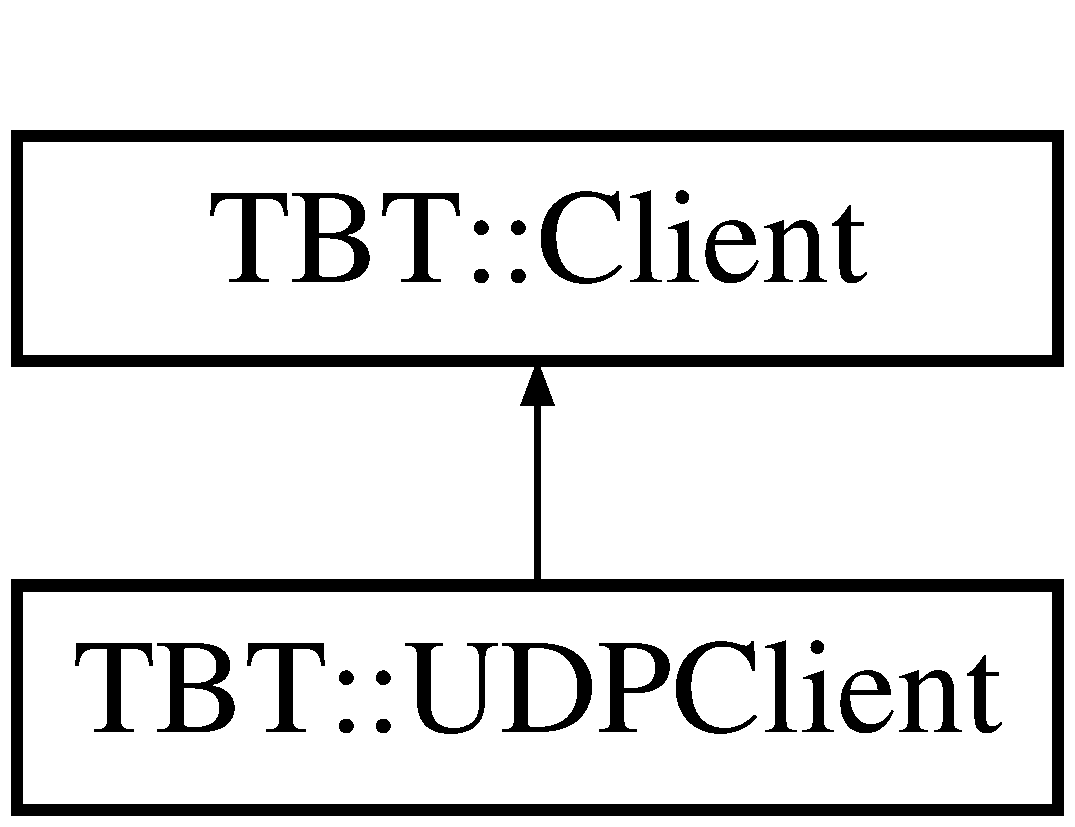
\includegraphics[height=2.000000cm]{classTBT_1_1UDPClient}
\end{center}
\end{figure}
\subsection*{Public Member Functions}
\begin{DoxyCompactItemize}
\item 
\mbox{\Hypertarget{classTBT_1_1UDPClient_a7b6f7858b9d3a7243bdd48fbf150b9f8}\label{classTBT_1_1UDPClient_a7b6f7858b9d3a7243bdd48fbf150b9f8}} 
{\bfseries U\+D\+P\+Client} (\hyperlink{classTBT_1_1UDPClientInterface}{U\+D\+P\+Client\+Interface} $\ast$pinterface, const sockaddr\+\_\+in \&address)
\item 
\mbox{\Hypertarget{classTBT_1_1UDPClient_aaf8b77e98494585ea3c44c9e89ec04ec}\label{classTBT_1_1UDPClient_aaf8b77e98494585ea3c44c9e89ec04ec}} 
virtual void {\bfseries broadcast\+Power\+State\+Change} (Power\+State new\+State)
\item 
\mbox{\Hypertarget{classTBT_1_1UDPClient_a90c650259501f341f531ede72210624a}\label{classTBT_1_1UDPClient_a90c650259501f341f531ede72210624a}} 
virtual void {\bfseries broadcast\+Loc\+Info\+Changed} (\hyperlink{classTBT_1_1LocDecoder}{Loc\+Decoder} $\ast$p\+Loc)
\item 
\mbox{\Hypertarget{classTBT_1_1UDPClient_aad30cea06b570b6a5e688710cfd53100}\label{classTBT_1_1UDPClient_aad30cea06b570b6a5e688710cfd53100}} 
virtual void {\bfseries broadcast\+Emergency\+Stop} (bool state)
\item 
\mbox{\Hypertarget{classTBT_1_1UDPClient_a8471b71655c61bf074b70b62a6dffbf1}\label{classTBT_1_1UDPClient_a8471b71655c61bf074b70b62a6dffbf1}} 
const sockaddr\+\_\+in \& {\bfseries get\+Address} (void)
\item 
\mbox{\Hypertarget{classTBT_1_1UDPClient_a18da0bdc657f707f4c0af6cd3b1e6031}\label{classTBT_1_1UDPClient_a18da0bdc657f707f4c0af6cd3b1e6031}} 
uint32\+\_\+t {\bfseries get\+Broadcast\+Flags} (void)
\item 
\mbox{\Hypertarget{classTBT_1_1UDPClient_a23a0b0ecf47f8a2fe018a570f46ecdfe}\label{classTBT_1_1UDPClient_a23a0b0ecf47f8a2fe018a570f46ecdfe}} 
void {\bfseries set\+Broadcast\+Flags} (uint32\+\_\+t new\+Flags)
\end{DoxyCompactItemize}
\subsection*{Protected Attributes}
\begin{DoxyCompactItemize}
\item 
\mbox{\Hypertarget{classTBT_1_1UDPClient_a880ede9d0208905a251bbfd221646e3b}\label{classTBT_1_1UDPClient_a880ede9d0208905a251bbfd221646e3b}} 
const sockaddr\+\_\+in {\bfseries m\+\_\+\+Address}
\item 
\mbox{\Hypertarget{classTBT_1_1UDPClient_aef66ad83fa20b995152c6f41cb8ba91f}\label{classTBT_1_1UDPClient_aef66ad83fa20b995152c6f41cb8ba91f}} 
int {\bfseries m\+\_\+\+My\+Socket}
\item 
\mbox{\Hypertarget{classTBT_1_1UDPClient_a91eb8f34a9606428eba7230c2bfdb6f6}\label{classTBT_1_1UDPClient_a91eb8f34a9606428eba7230c2bfdb6f6}} 
uint32\+\_\+t {\bfseries m\+\_\+\+Broadcast\+Flags}
\end{DoxyCompactItemize}


The documentation for this class was generated from the following files\+:\begin{DoxyCompactItemize}
\item 
U\+D\+P\+Client.\+h\item 
U\+D\+P\+Client.\+cpp\end{DoxyCompactItemize}

\hypertarget{classTBT_1_1UDPClientInterface}{}\section{T\+BT\+:\+:U\+D\+P\+Client\+Interface Class Reference}
\label{classTBT_1_1UDPClientInterface}\index{T\+B\+T\+::\+U\+D\+P\+Client\+Interface@{T\+B\+T\+::\+U\+D\+P\+Client\+Interface}}
Inheritance diagram for T\+BT\+:\+:U\+D\+P\+Client\+Interface\+:\begin{figure}[H]
\begin{center}
\leavevmode
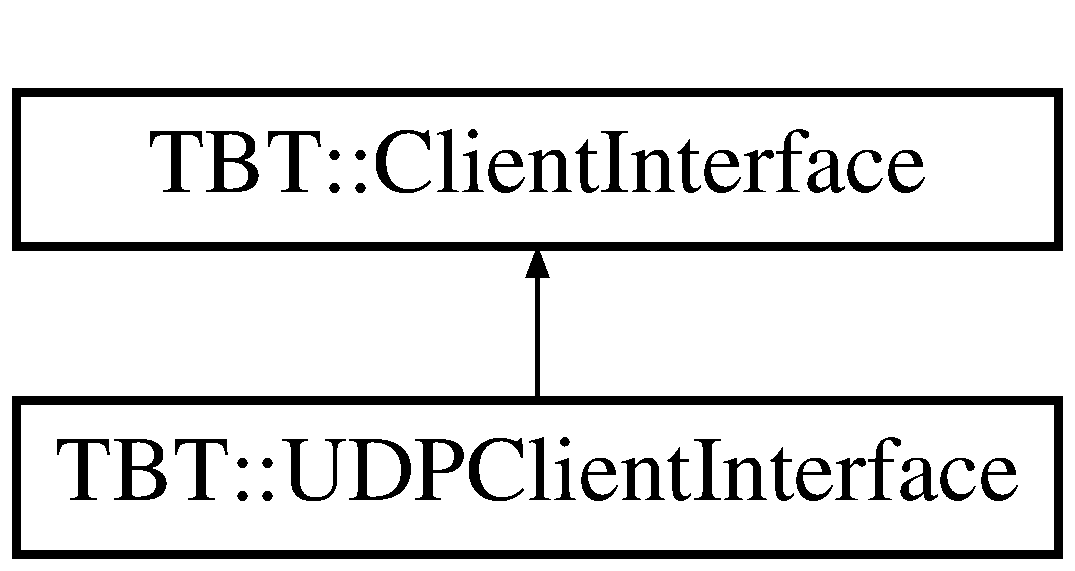
\includegraphics[height=2.000000cm]{classTBT_1_1UDPClientInterface}
\end{center}
\end{figure}
\subsection*{Public Member Functions}
\begin{DoxyCompactItemize}
\item 
\mbox{\Hypertarget{classTBT_1_1UDPClientInterface_ad03356f6abf16596c181851e9fcaf7a9}\label{classTBT_1_1UDPClientInterface_ad03356f6abf16596c181851e9fcaf7a9}} 
{\bfseries U\+D\+P\+Client\+Interface} (\hyperlink{classTBT_1_1Manager}{Manager} $\ast$p\+Manager, const in\+\_\+port\+\_\+t \&port=21105)
\item 
\mbox{\Hypertarget{classTBT_1_1UDPClientInterface_ac25b06823d045631f3c7b76e9c50f22e}\label{classTBT_1_1UDPClientInterface_ac25b06823d045631f3c7b76e9c50f22e}} 
int {\bfseries get\+My\+Socket} (void)
\item 
\mbox{\Hypertarget{classTBT_1_1UDPClientInterface_ad65d92928ce6f459c371c44c5576dbcc}\label{classTBT_1_1UDPClientInterface_ad65d92928ce6f459c371c44c5576dbcc}} 
virtual void {\bfseries broadcast\+Power\+State\+Change} (Power\+State new\+State)
\item 
\mbox{\Hypertarget{classTBT_1_1UDPClientInterface_af4e63115b3156b151d4dfd50342b36e7}\label{classTBT_1_1UDPClientInterface_af4e63115b3156b151d4dfd50342b36e7}} 
virtual void {\bfseries broadcast\+Loc\+Info\+Change} (\hyperlink{classTBT_1_1LocDecoder}{Loc\+Decoder} $\ast$p\+Loc)
\item 
\mbox{\Hypertarget{classTBT_1_1UDPClientInterface_a7fca1a79378823f67b0f23bbd59dc041}\label{classTBT_1_1UDPClientInterface_a7fca1a79378823f67b0f23bbd59dc041}} 
virtual void {\bfseries broadcast\+Emergency\+Stop} (bool state)
\end{DoxyCompactItemize}
\subsection*{Protected Member Functions}
\begin{DoxyCompactItemize}
\item 
\mbox{\Hypertarget{classTBT_1_1UDPClientInterface_aea926878d35ed4b37143e320143a84df}\label{classTBT_1_1UDPClientInterface_aea926878d35ed4b37143e320143a84df}} 
\hyperlink{classTBT_1_1UDPClient}{U\+D\+P\+Client} $\ast$ {\bfseries find\+Client} (const sockaddr\+\_\+in \&address)
\item 
\mbox{\Hypertarget{classTBT_1_1UDPClientInterface_a1a80ed1e5670443bc35691c9f3d5ff72}\label{classTBT_1_1UDPClientInterface_a1a80ed1e5670443bc35691c9f3d5ff72}} 
bool {\bfseries remove\+Client} (\hyperlink{classTBT_1_1UDPClient}{U\+D\+P\+Client} $\ast$p\+Client)
\end{DoxyCompactItemize}
\subsection*{Additional Inherited Members}


The documentation for this class was generated from the following files\+:\begin{DoxyCompactItemize}
\item 
U\+D\+P\+Client\+Interface.\+h\item 
U\+D\+P\+Client\+Interface.\+cpp\end{DoxyCompactItemize}

\hypertarget{classJson_1_1Value}{}\section{Json\+:\+:Value Class Reference}
\label{classJson_1_1Value}\index{Json\+::\+Value@{Json\+::\+Value}}


Represents a \href{http://www.json.org}{\tt J\+S\+ON} value.  




{\ttfamily \#include $<$json.\+h$>$}

\subsection*{Public Types}
\begin{DoxyCompactItemize}
\item 
\mbox{\Hypertarget{classJson_1_1Value_a9ae9069983fc38f1928d76f9c79ac64d}\label{classJson_1_1Value_a9ae9069983fc38f1928d76f9c79ac64d}} 
typedef std\+::vector$<$ J\+S\+O\+N\+C\+P\+P\+\_\+\+S\+T\+R\+I\+NG $>$ {\bfseries Members}
\item 
\mbox{\Hypertarget{classJson_1_1Value_a341cdf2e01f8b3c5b7317aa2f0768c53}\label{classJson_1_1Value_a341cdf2e01f8b3c5b7317aa2f0768c53}} 
typedef \hyperlink{classJson_1_1ValueIterator}{Value\+Iterator} {\bfseries iterator}
\item 
\mbox{\Hypertarget{classJson_1_1Value_af92282ca92b58b320debd486afb7696a}\label{classJson_1_1Value_af92282ca92b58b320debd486afb7696a}} 
typedef \hyperlink{classJson_1_1ValueConstIterator}{Value\+Const\+Iterator} {\bfseries const\+\_\+iterator}
\item 
\mbox{\Hypertarget{classJson_1_1Value_a0933d59b45793ae4aade1757c322a98d}\label{classJson_1_1Value_a0933d59b45793ae4aade1757c322a98d}} 
typedef Json\+::\+U\+Int {\bfseries U\+Int}
\item 
\mbox{\Hypertarget{classJson_1_1Value_abdf7a7ff73eb130ffcab28504ffdb405}\label{classJson_1_1Value_abdf7a7ff73eb130ffcab28504ffdb405}} 
typedef Json\+::\+Int {\bfseries Int}
\item 
\mbox{\Hypertarget{classJson_1_1Value_a8b62564be8c087c6d18de180ff4e13e3}\label{classJson_1_1Value_a8b62564be8c087c6d18de180ff4e13e3}} 
typedef Json\+::\+U\+Int64 {\bfseries U\+Int64}
\item 
\mbox{\Hypertarget{classJson_1_1Value_a1b86af9f85f0f1baa972c3319fa22695}\label{classJson_1_1Value_a1b86af9f85f0f1baa972c3319fa22695}} 
typedef Json\+::\+Int64 {\bfseries Int64}
\item 
\mbox{\Hypertarget{classJson_1_1Value_a1cbb82642ed05109b9833e49f042ece7}\label{classJson_1_1Value_a1cbb82642ed05109b9833e49f042ece7}} 
typedef Json\+::\+Largest\+Int {\bfseries Largest\+Int}
\item 
\mbox{\Hypertarget{classJson_1_1Value_a6682a3684d635e03fc06ba229fa24eec}\label{classJson_1_1Value_a6682a3684d635e03fc06ba229fa24eec}} 
typedef Json\+::\+Largest\+U\+Int {\bfseries Largest\+U\+Int}
\item 
\mbox{\Hypertarget{classJson_1_1Value_a184a91566cccca7b819240f0d5561c7d}\label{classJson_1_1Value_a184a91566cccca7b819240f0d5561c7d}} 
typedef Json\+::\+Array\+Index {\bfseries Array\+Index}
\item 
\mbox{\Hypertarget{classJson_1_1Value_a9e071ef3c135a2c9602e893b6005d0f7}\label{classJson_1_1Value_a9e071ef3c135a2c9602e893b6005d0f7}} 
typedef std\+::string {\bfseries value\+\_\+type}
\item 
\mbox{\Hypertarget{classJson_1_1Value_a08b6c80c3af7071d908dabf044de5388}\label{classJson_1_1Value_a08b6c80c3af7071d908dabf044de5388}} 
typedef std\+::map$<$ C\+Z\+String, \hyperlink{classJson_1_1Value}{Value} $>$ {\bfseries Object\+Values}
\end{DoxyCompactItemize}
\subsection*{Public Member Functions}
\begin{DoxyCompactItemize}
\item 
\hyperlink{classJson_1_1Value_ada6ba1369448fb0240bccc36efaa46f7}{Value} (\hyperlink{namespaceJson_a7d654b75c16a57007925868e38212b4e}{Value\+Type} type=\hyperlink{namespaceJson_a7d654b75c16a57007925868e38212b4ea7d9899633b4409bd3fc107e6737f8391}{null\+Value})
\begin{DoxyCompactList}\small\item\em Create a default \hyperlink{classJson_1_1Value}{Value} of the given type. \end{DoxyCompactList}\item 
\mbox{\Hypertarget{classJson_1_1Value_a4744ae571fcf34f4b16a2257b3b3b585}\label{classJson_1_1Value_a4744ae571fcf34f4b16a2257b3b3b585}} 
{\bfseries Value} (Int value)
\item 
\mbox{\Hypertarget{classJson_1_1Value_ae67a857b01286e3499a87e95be848d20}\label{classJson_1_1Value_ae67a857b01286e3499a87e95be848d20}} 
{\bfseries Value} (U\+Int value)
\item 
\mbox{\Hypertarget{classJson_1_1Value_ab1cdc3d9a4d4cc03fa01439d43ceb1b5}\label{classJson_1_1Value_ab1cdc3d9a4d4cc03fa01439d43ceb1b5}} 
{\bfseries Value} (Int64 value)
\item 
\mbox{\Hypertarget{classJson_1_1Value_a8adda58d5ae17bf7ca6a53bab4a7b69c}\label{classJson_1_1Value_a8adda58d5ae17bf7ca6a53bab4a7b69c}} 
{\bfseries Value} (U\+Int64 value)
\item 
\mbox{\Hypertarget{classJson_1_1Value_a32228cc84d83200cca8441451997996c}\label{classJson_1_1Value_a32228cc84d83200cca8441451997996c}} 
{\bfseries Value} (double value)
\item 
\mbox{\Hypertarget{classJson_1_1Value_ad87b849356816aca75995dd07302e49d}\label{classJson_1_1Value_ad87b849356816aca75995dd07302e49d}} 
\hyperlink{classJson_1_1Value_ad87b849356816aca75995dd07302e49d}{Value} (const char $\ast$value)
\begin{DoxyCompactList}\small\item\em Copy til first 0. (N\+U\+LL causes to seg-\/fault.) \end{DoxyCompactList}\item 
\mbox{\Hypertarget{classJson_1_1Value_a39fa09d1902efbd4350e1236db920571}\label{classJson_1_1Value_a39fa09d1902efbd4350e1236db920571}} 
\hyperlink{classJson_1_1Value_a39fa09d1902efbd4350e1236db920571}{Value} (const char $\ast$begin, const char $\ast$end)
\begin{DoxyCompactList}\small\item\em Copy all, incl zeroes. \end{DoxyCompactList}\item 
\hyperlink{classJson_1_1Value_a081830e95f88a37054da7e46c65b0766}{Value} (const \hyperlink{classJson_1_1StaticString}{Static\+String} \&value)
\begin{DoxyCompactList}\small\item\em Constructs a value from a static string. \end{DoxyCompactList}\item 
\mbox{\Hypertarget{classJson_1_1Value_a89ef37969ff7c6eb3a7afcca03d4cd4a}\label{classJson_1_1Value_a89ef37969ff7c6eb3a7afcca03d4cd4a}} 
\hyperlink{classJson_1_1Value_a89ef37969ff7c6eb3a7afcca03d4cd4a}{Value} (const J\+S\+O\+N\+C\+P\+P\+\_\+\+S\+T\+R\+I\+NG \&value)
\begin{DoxyCompactList}\small\item\em Copy data() til \hyperlink{classJson_1_1Value_a0ec2808e1d7efa4e9fad938d6667be44}{size()}. Embedded zeroes too. \end{DoxyCompactList}\item 
\mbox{\Hypertarget{classJson_1_1Value_a350a31ea4a30d384994b0bc010b17495}\label{classJson_1_1Value_a350a31ea4a30d384994b0bc010b17495}} 
{\bfseries Value} (bool value)
\item 
\mbox{\Hypertarget{classJson_1_1Value_a436dfd3670f95fd665f680eba5cebcf0}\label{classJson_1_1Value_a436dfd3670f95fd665f680eba5cebcf0}} 
\hyperlink{classJson_1_1Value_a436dfd3670f95fd665f680eba5cebcf0}{Value} (const \hyperlink{classJson_1_1Value}{Value} \&other)
\begin{DoxyCompactList}\small\item\em Deep copy. \end{DoxyCompactList}\item 
\hyperlink{classJson_1_1Value}{Value} \& \hyperlink{classJson_1_1Value_a795acb28772da4c5d85ae8f4af36c69f}{operator=} (\hyperlink{classJson_1_1Value}{Value} other)
\item 
\mbox{\Hypertarget{classJson_1_1Value_aab841120d78e296e1bc06a373345e822}\label{classJson_1_1Value_aab841120d78e296e1bc06a373345e822}} 
void \hyperlink{classJson_1_1Value_aab841120d78e296e1bc06a373345e822}{swap} (\hyperlink{classJson_1_1Value}{Value} \&other)
\begin{DoxyCompactList}\small\item\em Swap everything. \end{DoxyCompactList}\item 
\mbox{\Hypertarget{classJson_1_1Value_a5263476047f20e2fc6de470e4de34fe5}\label{classJson_1_1Value_a5263476047f20e2fc6de470e4de34fe5}} 
void \hyperlink{classJson_1_1Value_a5263476047f20e2fc6de470e4de34fe5}{swap\+Payload} (\hyperlink{classJson_1_1Value}{Value} \&other)
\begin{DoxyCompactList}\small\item\em Swap values but leave comments and source offsets in place. \end{DoxyCompactList}\item 
\mbox{\Hypertarget{classJson_1_1Value_a1b2c6379664d91b9f1bcd4d1853e5970}\label{classJson_1_1Value_a1b2c6379664d91b9f1bcd4d1853e5970}} 
void \hyperlink{classJson_1_1Value_a1b2c6379664d91b9f1bcd4d1853e5970}{copy} (const \hyperlink{classJson_1_1Value}{Value} \&other)
\begin{DoxyCompactList}\small\item\em copy everything. \end{DoxyCompactList}\item 
\mbox{\Hypertarget{classJson_1_1Value_ab504d299cfaa440392037fa8a3c54064}\label{classJson_1_1Value_ab504d299cfaa440392037fa8a3c54064}} 
void \hyperlink{classJson_1_1Value_ab504d299cfaa440392037fa8a3c54064}{copy\+Payload} (const \hyperlink{classJson_1_1Value}{Value} \&other)
\begin{DoxyCompactList}\small\item\em copy values but leave comments and source offsets in place. \end{DoxyCompactList}\item 
\mbox{\Hypertarget{classJson_1_1Value_a8ce61157a011894f0252ceed232312de}\label{classJson_1_1Value_a8ce61157a011894f0252ceed232312de}} 
\hyperlink{namespaceJson_a7d654b75c16a57007925868e38212b4e}{Value\+Type} {\bfseries type} () const
\item 
\mbox{\Hypertarget{classJson_1_1Value_aac6bd14155b88ed2d39ef54820b39e49}\label{classJson_1_1Value_aac6bd14155b88ed2d39ef54820b39e49}} 
bool \hyperlink{classJson_1_1Value_aac6bd14155b88ed2d39ef54820b39e49}{operator$<$} (const \hyperlink{classJson_1_1Value}{Value} \&other) const
\begin{DoxyCompactList}\small\item\em Compare payload only, not comments etc. \end{DoxyCompactList}\item 
\mbox{\Hypertarget{classJson_1_1Value_a40c411a320a416d5eac0052b36211286}\label{classJson_1_1Value_a40c411a320a416d5eac0052b36211286}} 
bool {\bfseries operator$<$=} (const \hyperlink{classJson_1_1Value}{Value} \&other) const
\item 
\mbox{\Hypertarget{classJson_1_1Value_afe2c3e52df60b9622cbd8358b74bdbf5}\label{classJson_1_1Value_afe2c3e52df60b9622cbd8358b74bdbf5}} 
bool {\bfseries operator$>$=} (const \hyperlink{classJson_1_1Value}{Value} \&other) const
\item 
\mbox{\Hypertarget{classJson_1_1Value_a4646c2f0764908c0972160c7c2ebe567}\label{classJson_1_1Value_a4646c2f0764908c0972160c7c2ebe567}} 
bool {\bfseries operator$>$} (const \hyperlink{classJson_1_1Value}{Value} \&other) const
\item 
\mbox{\Hypertarget{classJson_1_1Value_a16f9250e30d5c4505cd11137c564a764}\label{classJson_1_1Value_a16f9250e30d5c4505cd11137c564a764}} 
bool {\bfseries operator==} (const \hyperlink{classJson_1_1Value}{Value} \&other) const
\item 
\mbox{\Hypertarget{classJson_1_1Value_a86e95be072e515c48abc61dec63a1689}\label{classJson_1_1Value_a86e95be072e515c48abc61dec63a1689}} 
bool {\bfseries operator!=} (const \hyperlink{classJson_1_1Value}{Value} \&other) const
\item 
\mbox{\Hypertarget{classJson_1_1Value_aefa4464ca1bb0bcc9a87b38ed62ca2e0}\label{classJson_1_1Value_aefa4464ca1bb0bcc9a87b38ed62ca2e0}} 
int {\bfseries compare} (const \hyperlink{classJson_1_1Value}{Value} \&other) const
\item 
\mbox{\Hypertarget{classJson_1_1Value_a16668c8db7ef0a5de040012f0dfd84b0}\label{classJson_1_1Value_a16668c8db7ef0a5de040012f0dfd84b0}} 
const char $\ast$ \hyperlink{classJson_1_1Value_a16668c8db7ef0a5de040012f0dfd84b0}{as\+C\+String} () const
\begin{DoxyCompactList}\small\item\em Embedded zeroes could cause you trouble! \end{DoxyCompactList}\item 
\mbox{\Hypertarget{classJson_1_1Value_ae3f9b0d38f820ccdd8888aa92ea6e792}\label{classJson_1_1Value_ae3f9b0d38f820ccdd8888aa92ea6e792}} 
J\+S\+O\+N\+C\+P\+P\+\_\+\+S\+T\+R\+I\+NG \hyperlink{classJson_1_1Value_ae3f9b0d38f820ccdd8888aa92ea6e792}{as\+String} () const
\begin{DoxyCompactList}\small\item\em Embedded zeroes are possible. \end{DoxyCompactList}\item 
bool \hyperlink{classJson_1_1Value_a2e1b7be6bde2fe23f15290d9ddbbdf8a}{get\+String} (char const $\ast$$\ast$begin, char const $\ast$$\ast$end) const
\item 
\mbox{\Hypertarget{classJson_1_1Value_a614d635bc248a592593feb322cd15ab8}\label{classJson_1_1Value_a614d635bc248a592593feb322cd15ab8}} 
Int {\bfseries as\+Int} () const
\item 
\mbox{\Hypertarget{classJson_1_1Value_a74b305583ec3aacf4f9dd06e799dc265}\label{classJson_1_1Value_a74b305583ec3aacf4f9dd06e799dc265}} 
U\+Int {\bfseries as\+U\+Int} () const
\item 
\mbox{\Hypertarget{classJson_1_1Value_aa647ac4fe51a2e325c063ebe32262b44}\label{classJson_1_1Value_aa647ac4fe51a2e325c063ebe32262b44}} 
Int64 {\bfseries as\+Int64} () const
\item 
\mbox{\Hypertarget{classJson_1_1Value_a0e44a5a4cd0c099f9570dfa25813eb60}\label{classJson_1_1Value_a0e44a5a4cd0c099f9570dfa25813eb60}} 
U\+Int64 {\bfseries as\+U\+Int64} () const
\item 
\mbox{\Hypertarget{classJson_1_1Value_ab16f2ea2a117a1b3b576acab8b6a700d}\label{classJson_1_1Value_ab16f2ea2a117a1b3b576acab8b6a700d}} 
Largest\+Int {\bfseries as\+Largest\+Int} () const
\item 
\mbox{\Hypertarget{classJson_1_1Value_ad03548101e0bf3d2d9eac75c64a0b8d7}\label{classJson_1_1Value_ad03548101e0bf3d2d9eac75c64a0b8d7}} 
Largest\+U\+Int {\bfseries as\+Largest\+U\+Int} () const
\item 
\mbox{\Hypertarget{classJson_1_1Value_af3a4d10bf575fabdc5440a7135c9649c}\label{classJson_1_1Value_af3a4d10bf575fabdc5440a7135c9649c}} 
float {\bfseries as\+Float} () const
\item 
\mbox{\Hypertarget{classJson_1_1Value_afd24002a18aef907ad746b1cb9eda0a2}\label{classJson_1_1Value_afd24002a18aef907ad746b1cb9eda0a2}} 
double {\bfseries as\+Double} () const
\item 
\mbox{\Hypertarget{classJson_1_1Value_ab693fb7b9b1595bb0adc49658bbf780d}\label{classJson_1_1Value_ab693fb7b9b1595bb0adc49658bbf780d}} 
bool {\bfseries as\+Bool} () const
\item 
\mbox{\Hypertarget{classJson_1_1Value_abde4070e21e46dc4f8203f66582cb19f}\label{classJson_1_1Value_abde4070e21e46dc4f8203f66582cb19f}} 
bool {\bfseries is\+Null} () const
\item 
\mbox{\Hypertarget{classJson_1_1Value_ab1f02651cb89d0f18b63a036959391ba}\label{classJson_1_1Value_ab1f02651cb89d0f18b63a036959391ba}} 
bool {\bfseries is\+Bool} () const
\item 
\mbox{\Hypertarget{classJson_1_1Value_aff51d8b52979ca06cf9d909accd5f695}\label{classJson_1_1Value_aff51d8b52979ca06cf9d909accd5f695}} 
bool {\bfseries is\+Int} () const
\item 
\mbox{\Hypertarget{classJson_1_1Value_a4a81fb3c3acdbb68b2e2f30836a4f53e}\label{classJson_1_1Value_a4a81fb3c3acdbb68b2e2f30836a4f53e}} 
bool {\bfseries is\+Int64} () const
\item 
\mbox{\Hypertarget{classJson_1_1Value_abdda463d3269015f883587349726cfbc}\label{classJson_1_1Value_abdda463d3269015f883587349726cfbc}} 
bool {\bfseries is\+U\+Int} () const
\item 
\mbox{\Hypertarget{classJson_1_1Value_a883576e35cb03a785258edb56777a2de}\label{classJson_1_1Value_a883576e35cb03a785258edb56777a2de}} 
bool {\bfseries is\+U\+Int64} () const
\item 
\mbox{\Hypertarget{classJson_1_1Value_ab6798954f6e80281cf22708ef45198a7}\label{classJson_1_1Value_ab6798954f6e80281cf22708ef45198a7}} 
bool {\bfseries is\+Integral} () const
\item 
\mbox{\Hypertarget{classJson_1_1Value_a4a2e2a790e19a1c09fc5dd12d7ad47b5}\label{classJson_1_1Value_a4a2e2a790e19a1c09fc5dd12d7ad47b5}} 
bool {\bfseries is\+Double} () const
\item 
\mbox{\Hypertarget{classJson_1_1Value_af961a000cd203c895e44c195ab39b866}\label{classJson_1_1Value_af961a000cd203c895e44c195ab39b866}} 
bool {\bfseries is\+Numeric} () const
\item 
\mbox{\Hypertarget{classJson_1_1Value_a71e1f82cf1c3eaf969d400dcffb163a6}\label{classJson_1_1Value_a71e1f82cf1c3eaf969d400dcffb163a6}} 
bool {\bfseries is\+String} () const
\item 
\mbox{\Hypertarget{classJson_1_1Value_a1627eb9d6568d6d0252fa8bb711c0a59}\label{classJson_1_1Value_a1627eb9d6568d6d0252fa8bb711c0a59}} 
bool {\bfseries is\+Array} () const
\item 
\mbox{\Hypertarget{classJson_1_1Value_a8cf96c0f2a552051fcfc78ffee60e037}\label{classJson_1_1Value_a8cf96c0f2a552051fcfc78ffee60e037}} 
bool {\bfseries is\+Object} () const
\item 
\mbox{\Hypertarget{classJson_1_1Value_af1ee6be27a96a7d12128efdd60deb54d}\label{classJson_1_1Value_af1ee6be27a96a7d12128efdd60deb54d}} 
bool {\bfseries is\+Convertible\+To} (\hyperlink{namespaceJson_a7d654b75c16a57007925868e38212b4e}{Value\+Type} other) const
\item 
\mbox{\Hypertarget{classJson_1_1Value_a0ec2808e1d7efa4e9fad938d6667be44}\label{classJson_1_1Value_a0ec2808e1d7efa4e9fad938d6667be44}} 
Array\+Index \hyperlink{classJson_1_1Value_a0ec2808e1d7efa4e9fad938d6667be44}{size} () const
\begin{DoxyCompactList}\small\item\em Number of values in array or object. \end{DoxyCompactList}\item 
\mbox{\Hypertarget{classJson_1_1Value_a0519a551e37ee6665d74742b3f96bab3}\label{classJson_1_1Value_a0519a551e37ee6665d74742b3f96bab3}} 
bool \hyperlink{classJson_1_1Value_a0519a551e37ee6665d74742b3f96bab3}{empty} () const
\begin{DoxyCompactList}\small\item\em Return true if empty array, empty object, or null; otherwise, false. \end{DoxyCompactList}\item 
\mbox{\Hypertarget{classJson_1_1Value_a731b89fb4764c39ce2328e1707c822b9}\label{classJson_1_1Value_a731b89fb4764c39ce2328e1707c822b9}} 
bool \hyperlink{classJson_1_1Value_a731b89fb4764c39ce2328e1707c822b9}{operator!} () const
\begin{DoxyCompactList}\small\item\em Return is\+Null() \end{DoxyCompactList}\item 
void \hyperlink{classJson_1_1Value_a501a4d67e6c875255c2ecc03ccd2019b}{clear} ()
\item 
void \hyperlink{classJson_1_1Value_aa284353271ada427dbfa04a42f2be407}{resize} (Array\+Index \hyperlink{classJson_1_1Value_a0ec2808e1d7efa4e9fad938d6667be44}{size})
\item 
\hyperlink{classJson_1_1Value}{Value} \& \hyperlink{classJson_1_1Value_a7d99f5dba388cdaa152ce6ef933d64ef}{operator\mbox{[}$\,$\mbox{]}} (Array\+Index index)
\item 
\hyperlink{classJson_1_1Value}{Value} \& \hyperlink{classJson_1_1Value_ac9182982c361e0ab621134d406e5f250}{operator\mbox{[}$\,$\mbox{]}} (int index)
\item 
const \hyperlink{classJson_1_1Value}{Value} \& \hyperlink{classJson_1_1Value_a46607236038b29695ed80c15895271e4}{operator\mbox{[}$\,$\mbox{]}} (Array\+Index index) const
\item 
const \hyperlink{classJson_1_1Value}{Value} \& \hyperlink{classJson_1_1Value_a0b42557a95621a4676b46a21ffc5e949}{operator\mbox{[}$\,$\mbox{]}} (int index) const
\item 
\hyperlink{classJson_1_1Value}{Value} \hyperlink{classJson_1_1Value_a034eb7bf85a44fa759bdaa232788ca66}{get} (Array\+Index index, const \hyperlink{classJson_1_1Value}{Value} \&default\+Value) const
\item 
\mbox{\Hypertarget{classJson_1_1Value_ac2928f174a6e081c1500c28c2d61ee93}\label{classJson_1_1Value_ac2928f174a6e081c1500c28c2d61ee93}} 
bool \hyperlink{classJson_1_1Value_ac2928f174a6e081c1500c28c2d61ee93}{is\+Valid\+Index} (Array\+Index index) const
\begin{DoxyCompactList}\small\item\em Return true if index $<$ \hyperlink{classJson_1_1Value_a0ec2808e1d7efa4e9fad938d6667be44}{size()}. \end{DoxyCompactList}\item 
\hyperlink{classJson_1_1Value}{Value} \& \hyperlink{classJson_1_1Value_a7e49ac977e4bcf59745a09d426669f75}{append} (const \hyperlink{classJson_1_1Value}{Value} \&value)
\begin{DoxyCompactList}\small\item\em Append value to array at the end. \end{DoxyCompactList}\item 
\hyperlink{classJson_1_1Value}{Value} \& \hyperlink{classJson_1_1Value_acb912f4ec40a25ea6eb387730885f3d9}{operator\mbox{[}$\,$\mbox{]}} (const char $\ast$key)
\item 
const \hyperlink{classJson_1_1Value}{Value} \& \hyperlink{classJson_1_1Value_a1b0498b7b2a520a68137f682d91abdd5}{operator\mbox{[}$\,$\mbox{]}} (const char $\ast$key) const
\item 
\hyperlink{classJson_1_1Value}{Value} \& \hyperlink{classJson_1_1Value_aedd1e152756a4cc8c1ebac0dd7aeeb78}{operator\mbox{[}$\,$\mbox{]}} (const J\+S\+O\+N\+C\+P\+P\+\_\+\+S\+T\+R\+I\+NG \&key)
\item 
const \hyperlink{classJson_1_1Value}{Value} \& \hyperlink{classJson_1_1Value_aba60f69dcd85e935aa85e7a517e03427}{operator\mbox{[}$\,$\mbox{]}} (const J\+S\+O\+N\+C\+P\+P\+\_\+\+S\+T\+R\+I\+NG \&key) const
\item 
\hyperlink{classJson_1_1Value}{Value} \& \hyperlink{classJson_1_1Value_ac3763d7d315ca65dc188e273722f7955}{operator\mbox{[}$\,$\mbox{]}} (const \hyperlink{classJson_1_1StaticString}{Static\+String} \&key)
\begin{DoxyCompactList}\small\item\em Access an object value by name, create a null member if it does not exist. \end{DoxyCompactList}\item 
\hyperlink{classJson_1_1Value}{Value} \hyperlink{classJson_1_1Value_a57de86629ed23246f14014fb6c44fa67}{get} (const char $\ast$key, const \hyperlink{classJson_1_1Value}{Value} \&default\+Value) const
\item 
\hyperlink{classJson_1_1Value}{Value} \hyperlink{classJson_1_1Value_aa59ed050e87e1d58d93671a38687f36c}{get} (const char $\ast$begin, const char $\ast$end, const \hyperlink{classJson_1_1Value}{Value} \&default\+Value) const
\item 
\hyperlink{classJson_1_1Value}{Value} \hyperlink{classJson_1_1Value_a7406e6af727c288bf8ab59945ece686a}{get} (const J\+S\+O\+N\+C\+P\+P\+\_\+\+S\+T\+R\+I\+NG \&key, const \hyperlink{classJson_1_1Value}{Value} \&default\+Value) const
\item 
\hyperlink{classJson_1_1Value}{Value} const  $\ast$ \hyperlink{classJson_1_1Value_afb007b9ce9b2cf9d5f667a07e5e0349f}{find} (char const $\ast$begin, char const $\ast$end) const
\item 
\hyperlink{classJson_1_1Value}{Value} const  $\ast$ \hyperlink{classJson_1_1Value_afeb7ff596a0929d90c5f2f3cffb413ed}{demand} (char const $\ast$begin, char const $\ast$end)
\item 
void \hyperlink{classJson_1_1Value_a92e165f04105d27a930fb3a18a053585}{remove\+Member} (const char $\ast$key)
\begin{DoxyCompactList}\small\item\em Remove and return the named member. \end{DoxyCompactList}\item 
void \hyperlink{classJson_1_1Value_a8a660202bbad35857b39e85bd35ec78a}{remove\+Member} (const J\+S\+O\+N\+C\+P\+P\+\_\+\+S\+T\+R\+I\+NG \&key)
\item 
bool \hyperlink{classJson_1_1Value_a708e599489adf30d65bf85a8ee16e6fb}{remove\+Member} (const char $\ast$key, \hyperlink{classJson_1_1Value}{Value} $\ast$removed)
\item 
bool \hyperlink{classJson_1_1Value_ae385ecef98427970df525ee876e9f54a}{remove\+Member} (J\+S\+O\+N\+C\+P\+P\+\_\+\+S\+T\+R\+I\+NG const \&key, \hyperlink{classJson_1_1Value}{Value} $\ast$removed)
\begin{DoxyCompactList}\small\item\em Remove the named map member. \end{DoxyCompactList}\item 
\mbox{\Hypertarget{classJson_1_1Value_a49c91af727d6b4eb0af02a81bb2def87}\label{classJson_1_1Value_a49c91af727d6b4eb0af02a81bb2def87}} 
bool \hyperlink{classJson_1_1Value_a49c91af727d6b4eb0af02a81bb2def87}{remove\+Member} (const char $\ast$begin, const char $\ast$end, \hyperlink{classJson_1_1Value}{Value} $\ast$removed)
\begin{DoxyCompactList}\small\item\em Same as \hyperlink{classJson_1_1Value_ae385ecef98427970df525ee876e9f54a}{remove\+Member(\+J\+S\+O\+N\+C\+P\+P\+\_\+\+S\+T\+R\+I\+N\+G const\& key, Value$\ast$ removed)} \end{DoxyCompactList}\item 
bool \hyperlink{classJson_1_1Value_ae9e67e08a85a2f3be3396ec0f4c47f65}{remove\+Index} (Array\+Index i, \hyperlink{classJson_1_1Value}{Value} $\ast$removed)
\begin{DoxyCompactList}\small\item\em Remove the indexed array element. \end{DoxyCompactList}\item 
bool \hyperlink{classJson_1_1Value_ad6d4df2227321bab05e86667609a7fad}{is\+Member} (const char $\ast$key) const
\item 
bool \hyperlink{classJson_1_1Value_a0c2cd838217b23ee6bde8135de1b30d9}{is\+Member} (const J\+S\+O\+N\+C\+P\+P\+\_\+\+S\+T\+R\+I\+NG \&key) const
\item 
\mbox{\Hypertarget{classJson_1_1Value_a2007e1e51f21f44ecf1f13e4a1c567b9}\label{classJson_1_1Value_a2007e1e51f21f44ecf1f13e4a1c567b9}} 
bool \hyperlink{classJson_1_1Value_a2007e1e51f21f44ecf1f13e4a1c567b9}{is\+Member} (const char $\ast$begin, const char $\ast$end) const
\begin{DoxyCompactList}\small\item\em Same as \hyperlink{classJson_1_1Value_a0c2cd838217b23ee6bde8135de1b30d9}{is\+Member(\+J\+S\+O\+N\+C\+P\+P\+\_\+\+S\+T\+R\+I\+N\+G const\& key)const}. \end{DoxyCompactList}\item 
Members \hyperlink{classJson_1_1Value_a79d7725dce6260317333e69022367ac9}{get\+Member\+Names} () const
\begin{DoxyCompactList}\small\item\em Return a list of the member names. \end{DoxyCompactList}\item 
void \hyperlink{classJson_1_1Value_a29f3a30f7e5d3af6f38d57999bf5b480}{set\+Comment} (const char $\ast$comment, \hyperlink{namespaceJson_a4fc417c23905b2ae9e2c47d197a45351}{Comment\+Placement} placement)
\item 
\mbox{\Hypertarget{classJson_1_1Value_a2900152a2887b410a9ddabe278b9d492}\label{classJson_1_1Value_a2900152a2887b410a9ddabe278b9d492}} 
void \hyperlink{classJson_1_1Value_a2900152a2887b410a9ddabe278b9d492}{set\+Comment} (const char $\ast$comment, size\+\_\+t len, \hyperlink{namespaceJson_a4fc417c23905b2ae9e2c47d197a45351}{Comment\+Placement} placement)
\begin{DoxyCompactList}\small\item\em Comments must be //... or /$\ast$ ... $\ast$/. \end{DoxyCompactList}\item 
\mbox{\Hypertarget{classJson_1_1Value_a2c5d13a5f45eb77e912008778e65b27f}\label{classJson_1_1Value_a2c5d13a5f45eb77e912008778e65b27f}} 
void \hyperlink{classJson_1_1Value_a2c5d13a5f45eb77e912008778e65b27f}{set\+Comment} (const J\+S\+O\+N\+C\+P\+P\+\_\+\+S\+T\+R\+I\+NG \&comment, \hyperlink{namespaceJson_a4fc417c23905b2ae9e2c47d197a45351}{Comment\+Placement} placement)
\begin{DoxyCompactList}\small\item\em Comments must be //... or /$\ast$ ... $\ast$/. \end{DoxyCompactList}\item 
\mbox{\Hypertarget{classJson_1_1Value_a65d8e3ab6a5871cbd019a3e0f0b944a3}\label{classJson_1_1Value_a65d8e3ab6a5871cbd019a3e0f0b944a3}} 
bool {\bfseries has\+Comment} (\hyperlink{namespaceJson_a4fc417c23905b2ae9e2c47d197a45351}{Comment\+Placement} placement) const
\item 
\mbox{\Hypertarget{classJson_1_1Value_a82817229a986f0b254e31d5c83066ffe}\label{classJson_1_1Value_a82817229a986f0b254e31d5c83066ffe}} 
J\+S\+O\+N\+C\+P\+P\+\_\+\+S\+T\+R\+I\+NG \hyperlink{classJson_1_1Value_a82817229a986f0b254e31d5c83066ffe}{get\+Comment} (\hyperlink{namespaceJson_a4fc417c23905b2ae9e2c47d197a45351}{Comment\+Placement} placement) const
\begin{DoxyCompactList}\small\item\em Include delimiters and embedded newlines. \end{DoxyCompactList}\item 
\mbox{\Hypertarget{classJson_1_1Value_a00154cc8662d7a845ed59e175c2496cb}\label{classJson_1_1Value_a00154cc8662d7a845ed59e175c2496cb}} 
J\+S\+O\+N\+C\+P\+P\+\_\+\+S\+T\+R\+I\+NG {\bfseries to\+Styled\+String} () const
\item 
\mbox{\Hypertarget{classJson_1_1Value_a015459a3950c198d63a2d3be8f5ae296}\label{classJson_1_1Value_a015459a3950c198d63a2d3be8f5ae296}} 
\hyperlink{classJson_1_1ValueConstIterator}{const\+\_\+iterator} {\bfseries begin} () const
\item 
\mbox{\Hypertarget{classJson_1_1Value_a3e443cd0ef24f7e028b175e47ee045e0}\label{classJson_1_1Value_a3e443cd0ef24f7e028b175e47ee045e0}} 
\hyperlink{classJson_1_1ValueConstIterator}{const\+\_\+iterator} {\bfseries end} () const
\item 
\mbox{\Hypertarget{classJson_1_1Value_a2d45bb2e68e8f22fe356d7d955ebd3c9}\label{classJson_1_1Value_a2d45bb2e68e8f22fe356d7d955ebd3c9}} 
\hyperlink{classJson_1_1ValueIterator}{iterator} {\bfseries begin} ()
\item 
\mbox{\Hypertarget{classJson_1_1Value_a2f961eff73f7f79cd29260b6cbd42558}\label{classJson_1_1Value_a2f961eff73f7f79cd29260b6cbd42558}} 
\hyperlink{classJson_1_1ValueIterator}{iterator} {\bfseries end} ()
\item 
\mbox{\Hypertarget{classJson_1_1Value_a92e32ea0f4f8a15853a3cf0beac9feb9}\label{classJson_1_1Value_a92e32ea0f4f8a15853a3cf0beac9feb9}} 
void {\bfseries set\+Offset\+Start} (ptrdiff\+\_\+t start)
\item 
\mbox{\Hypertarget{classJson_1_1Value_a5e4f5853fec138150c5df6004a8c2bcf}\label{classJson_1_1Value_a5e4f5853fec138150c5df6004a8c2bcf}} 
void {\bfseries set\+Offset\+Limit} (ptrdiff\+\_\+t limit)
\item 
\mbox{\Hypertarget{classJson_1_1Value_afa081dc764000951a1d8d6148155508e}\label{classJson_1_1Value_afa081dc764000951a1d8d6148155508e}} 
ptrdiff\+\_\+t {\bfseries get\+Offset\+Start} () const
\item 
\mbox{\Hypertarget{classJson_1_1Value_a2cdfa01935f87fcace90d450cbd2c0a4}\label{classJson_1_1Value_a2cdfa01935f87fcace90d450cbd2c0a4}} 
ptrdiff\+\_\+t {\bfseries get\+Offset\+Limit} () const
\end{DoxyCompactItemize}
\subsection*{Static Public Member Functions}
\begin{DoxyCompactItemize}
\item 
\mbox{\Hypertarget{classJson_1_1Value_af2f124567acc35d021a424e53ebdfcab}\label{classJson_1_1Value_af2f124567acc35d021a424e53ebdfcab}} 
static \hyperlink{classJson_1_1Value}{Value} const  \& \hyperlink{classJson_1_1Value_af2f124567acc35d021a424e53ebdfcab}{null\+Singleton} ()
\begin{DoxyCompactList}\small\item\em Prefer this to null or null\+Ref. \end{DoxyCompactList}\end{DoxyCompactItemize}
\subsection*{Static Public Attributes}
\begin{DoxyCompactItemize}
\item 
\mbox{\Hypertarget{classJson_1_1Value_a21ddb05b92c60c7548e928bf371e7d45}\label{classJson_1_1Value_a21ddb05b92c60c7548e928bf371e7d45}} 
static const \hyperlink{classJson_1_1Value}{Value} \& \hyperlink{classJson_1_1Value_a21ddb05b92c60c7548e928bf371e7d45}{null} = \hyperlink{classJson_1_1Value_af2f124567acc35d021a424e53ebdfcab}{Value\+::null\+Singleton}()
\begin{DoxyCompactList}\small\item\em We regret this reference to a global instance; prefer the simpler \hyperlink{classJson_1_1Value_ada6ba1369448fb0240bccc36efaa46f7}{Value()}. \end{DoxyCompactList}\item 
\mbox{\Hypertarget{classJson_1_1Value_aaee27e622f87266f861216d644603730}\label{classJson_1_1Value_aaee27e622f87266f861216d644603730}} 
static const \hyperlink{classJson_1_1Value}{Value} \& \hyperlink{classJson_1_1Value_aaee27e622f87266f861216d644603730}{null\+Ref} = \hyperlink{classJson_1_1Value_af2f124567acc35d021a424e53ebdfcab}{Value\+::null\+Singleton}()
\begin{DoxyCompactList}\small\item\em just a kludge for binary-\/compatibility; same as null \end{DoxyCompactList}\item 
\mbox{\Hypertarget{classJson_1_1Value_af91df130daa50dd43d2cd89e6ee67706}\label{classJson_1_1Value_af91df130daa50dd43d2cd89e6ee67706}} 
static const Largest\+Int \hyperlink{classJson_1_1Value_af91df130daa50dd43d2cd89e6ee67706}{min\+Largest\+Int} = Largest\+Int($\sim$(Largest\+U\+Int(-\/1) / 2))
\begin{DoxyCompactList}\small\item\em Minimum signed integer value that can be stored in a \hyperlink{classJson_1_1Value}{Json\+::\+Value}. \end{DoxyCompactList}\item 
\mbox{\Hypertarget{classJson_1_1Value_a8b4977696f13296fa8755c7953fafb2f}\label{classJson_1_1Value_a8b4977696f13296fa8755c7953fafb2f}} 
static const Largest\+Int \hyperlink{classJson_1_1Value_a8b4977696f13296fa8755c7953fafb2f}{max\+Largest\+Int} = Largest\+Int(Largest\+U\+Int(-\/1) / 2)
\begin{DoxyCompactList}\small\item\em Maximum signed integer value that can be stored in a \hyperlink{classJson_1_1Value}{Json\+::\+Value}. \end{DoxyCompactList}\item 
\mbox{\Hypertarget{classJson_1_1Value_a8ddb32d9d55fa5323ae5135639dc2e31}\label{classJson_1_1Value_a8ddb32d9d55fa5323ae5135639dc2e31}} 
static const Largest\+U\+Int \hyperlink{classJson_1_1Value_a8ddb32d9d55fa5323ae5135639dc2e31}{max\+Largest\+U\+Int} = Largest\+U\+Int(-\/1)
\begin{DoxyCompactList}\small\item\em Maximum unsigned integer value that can be stored in a \hyperlink{classJson_1_1Value}{Json\+::\+Value}. \end{DoxyCompactList}\item 
\mbox{\Hypertarget{classJson_1_1Value_a7df8a39e2502b8c92a6a41e3d752d2c8}\label{classJson_1_1Value_a7df8a39e2502b8c92a6a41e3d752d2c8}} 
static const Int \hyperlink{classJson_1_1Value_a7df8a39e2502b8c92a6a41e3d752d2c8}{min\+Int} = Int($\sim$(U\+Int(-\/1) / 2))
\begin{DoxyCompactList}\small\item\em Minimum signed int value that can be stored in a \hyperlink{classJson_1_1Value}{Json\+::\+Value}. \end{DoxyCompactList}\item 
\mbox{\Hypertarget{classJson_1_1Value_a978c799a8af3114ef7dab6fd0a310a1b}\label{classJson_1_1Value_a978c799a8af3114ef7dab6fd0a310a1b}} 
static const Int \hyperlink{classJson_1_1Value_a978c799a8af3114ef7dab6fd0a310a1b}{max\+Int} = Int(U\+Int(-\/1) / 2)
\begin{DoxyCompactList}\small\item\em Maximum signed int value that can be stored in a \hyperlink{classJson_1_1Value}{Json\+::\+Value}. \end{DoxyCompactList}\item 
\mbox{\Hypertarget{classJson_1_1Value_ac79e63ee68d3aa914bfd6988be669b87}\label{classJson_1_1Value_ac79e63ee68d3aa914bfd6988be669b87}} 
static const U\+Int \hyperlink{classJson_1_1Value_ac79e63ee68d3aa914bfd6988be669b87}{max\+U\+Int} = U\+Int(-\/1)
\begin{DoxyCompactList}\small\item\em Maximum unsigned int value that can be stored in a \hyperlink{classJson_1_1Value}{Json\+::\+Value}. \end{DoxyCompactList}\item 
\mbox{\Hypertarget{classJson_1_1Value_a815ef899bc312c93bc426511acfe31a7}\label{classJson_1_1Value_a815ef899bc312c93bc426511acfe31a7}} 
static const Int64 \hyperlink{classJson_1_1Value_a815ef899bc312c93bc426511acfe31a7}{min\+Int64} = Int64($\sim$(U\+Int64(-\/1) / 2))
\begin{DoxyCompactList}\small\item\em Minimum signed 64 bits int value that can be stored in a \hyperlink{classJson_1_1Value}{Json\+::\+Value}. \end{DoxyCompactList}\item 
\mbox{\Hypertarget{classJson_1_1Value_a4492634870b8c5709ce967b384ac6006}\label{classJson_1_1Value_a4492634870b8c5709ce967b384ac6006}} 
static const Int64 \hyperlink{classJson_1_1Value_a4492634870b8c5709ce967b384ac6006}{max\+Int64} = Int64(U\+Int64(-\/1) / 2)
\begin{DoxyCompactList}\small\item\em Maximum signed 64 bits int value that can be stored in a \hyperlink{classJson_1_1Value}{Json\+::\+Value}. \end{DoxyCompactList}\item 
\mbox{\Hypertarget{classJson_1_1Value_ae1eb89c305c39516696ff305cffa01da}\label{classJson_1_1Value_ae1eb89c305c39516696ff305cffa01da}} 
static const U\+Int64 \hyperlink{classJson_1_1Value_ae1eb89c305c39516696ff305cffa01da}{max\+U\+Int64} = U\+Int64(-\/1)
\begin{DoxyCompactList}\small\item\em Maximum unsigned 64 bits int value that can be stored in a \hyperlink{classJson_1_1Value}{Json\+::\+Value}. \end{DoxyCompactList}\end{DoxyCompactItemize}
\subsection*{Friends}
\begin{DoxyCompactItemize}
\item 
\mbox{\Hypertarget{classJson_1_1Value_ad016df56489e5d360735457afba2f649}\label{classJson_1_1Value_ad016df56489e5d360735457afba2f649}} 
class {\bfseries Value\+Iterator\+Base}
\end{DoxyCompactItemize}


\subsection{Detailed Description}
Represents a \href{http://www.json.org}{\tt J\+S\+ON} value. 

This class is a discriminated union wrapper that can represents a\+:
\begin{DoxyItemize}
\item signed integer \mbox{[}range\+: \hyperlink{classJson_1_1Value_a7df8a39e2502b8c92a6a41e3d752d2c8}{Value\+::min\+Int} -\/ \hyperlink{classJson_1_1Value_a978c799a8af3114ef7dab6fd0a310a1b}{Value\+::max\+Int}\mbox{]}
\item unsigned integer (range\+: 0 -\/ \hyperlink{classJson_1_1Value_ac79e63ee68d3aa914bfd6988be669b87}{Value\+::max\+U\+Int})
\item double
\item U\+T\+F-\/8 string
\item boolean
\item \textquotesingle{}null\textquotesingle{}
\item an ordered list of \hyperlink{classJson_1_1Value}{Value}
\item collection of name/value pairs (javascript object)
\end{DoxyItemize}

The type of the held value is represented by a \hyperlink{namespaceJson_a7d654b75c16a57007925868e38212b4e}{Value\+Type} and can be obtained using type().

Values of an \hyperlink{namespaceJson_a7d654b75c16a57007925868e38212b4eae8386dcfc36d1ae897745f7b4f77a1f6}{object\+Value} or \hyperlink{namespaceJson_a7d654b75c16a57007925868e38212b4eadc8f264f36b55b063c78126b335415f4}{array\+Value} can be accessed using \hyperlink{classJson_1_1Value_a7d99f5dba388cdaa152ce6ef933d64ef}{operator\mbox{[}$\,$\mbox{]}()} methods. Non-\/const methods will automatically create the a \hyperlink{namespaceJson_a7d654b75c16a57007925868e38212b4ea7d9899633b4409bd3fc107e6737f8391}{null\+Value} element if it does not exist. The sequence of an \hyperlink{namespaceJson_a7d654b75c16a57007925868e38212b4eadc8f264f36b55b063c78126b335415f4}{array\+Value} will be automatically resized and initialized with \hyperlink{namespaceJson_a7d654b75c16a57007925868e38212b4ea7d9899633b4409bd3fc107e6737f8391}{null\+Value}. \hyperlink{classJson_1_1Value_aa284353271ada427dbfa04a42f2be407}{resize()} can be used to enlarge or truncate an \hyperlink{namespaceJson_a7d654b75c16a57007925868e38212b4eadc8f264f36b55b063c78126b335415f4}{array\+Value}.

The \hyperlink{classJson_1_1Value_a034eb7bf85a44fa759bdaa232788ca66}{get()} methods can be used to obtain default value in the case the required element does not exist.

It is possible to iterate over the list of a \hyperlink{namespaceJson_a7d654b75c16a57007925868e38212b4eae8386dcfc36d1ae897745f7b4f77a1f6}{object\+Value} values using the \hyperlink{classJson_1_1Value_a79d7725dce6260317333e69022367ac9}{get\+Member\+Names()} method.

\begin{DoxyNote}{Note}
\hyperlink{classJson_1_1Value_ada6ba1369448fb0240bccc36efaa46f7}{Value} string-\/length fit in size\+\_\+t, but keys must be $<$ 2$^\wedge$30. (The reason is an implementation detail.) A \#\+Char\+Reader will raise an exception if a bound is exceeded to avoid security holes in your app, but the \hyperlink{classJson_1_1Value}{Value} A\+PI does {\itshape not} check bounds. That is the responsibility of the caller. 
\end{DoxyNote}


\subsection{Constructor \& Destructor Documentation}
\mbox{\Hypertarget{classJson_1_1Value_ada6ba1369448fb0240bccc36efaa46f7}\label{classJson_1_1Value_ada6ba1369448fb0240bccc36efaa46f7}} 
\index{Json\+::\+Value@{Json\+::\+Value}!Value@{Value}}
\index{Value@{Value}!Json\+::\+Value@{Json\+::\+Value}}
\subsubsection{\texorpdfstring{Value()}{Value()}\hspace{0.1cm}{\footnotesize\ttfamily [1/2]}}
{\footnotesize\ttfamily Json\+::\+Value\+::\+Value (\begin{DoxyParamCaption}\item[{\hyperlink{namespaceJson_a7d654b75c16a57007925868e38212b4e}{Value\+Type}}]{type = {\ttfamily \hyperlink{namespaceJson_a7d654b75c16a57007925868e38212b4ea7d9899633b4409bd3fc107e6737f8391}{null\+Value}} }\end{DoxyParamCaption})}



Create a default \hyperlink{classJson_1_1Value}{Value} of the given type. 

This is a very useful constructor. To create an empty array, pass array\+Value. To create an empty object, pass object\+Value. Another \hyperlink{classJson_1_1Value}{Value} can then be set to this one by assignment. This is useful since \hyperlink{classJson_1_1Value_a501a4d67e6c875255c2ecc03ccd2019b}{clear()} and \hyperlink{classJson_1_1Value_aa284353271ada427dbfa04a42f2be407}{resize()} will not alter types. \begin{DoxyVerb}Examples:
\end{DoxyVerb}
 
\begin{DoxyCode}
\hyperlink{classJson_1_1Value}{Json::Value} null\_value; \textcolor{comment}{// null}
\hyperlink{classJson_1_1Value}{Json::Value} arr\_value(\hyperlink{namespaceJson_a7d654b75c16a57007925868e38212b4eadc8f264f36b55b063c78126b335415f4}{Json::arrayValue}); \textcolor{comment}{// []}
\hyperlink{classJson_1_1Value}{Json::Value} obj\_value(\hyperlink{namespaceJson_a7d654b75c16a57007925868e38212b4eae8386dcfc36d1ae897745f7b4f77a1f6}{Json::objectValue}); \textcolor{comment}{// \{\}}
\end{DoxyCode}
 \mbox{\Hypertarget{classJson_1_1Value_a081830e95f88a37054da7e46c65b0766}\label{classJson_1_1Value_a081830e95f88a37054da7e46c65b0766}} 
\index{Json\+::\+Value@{Json\+::\+Value}!Value@{Value}}
\index{Value@{Value}!Json\+::\+Value@{Json\+::\+Value}}
\subsubsection{\texorpdfstring{Value()}{Value()}\hspace{0.1cm}{\footnotesize\ttfamily [2/2]}}
{\footnotesize\ttfamily Json\+::\+Value\+::\+Value (\begin{DoxyParamCaption}\item[{const \hyperlink{classJson_1_1StaticString}{Static\+String} \&}]{value }\end{DoxyParamCaption})}



Constructs a value from a static string. 

Like other value string constructor but do not duplicate the string for internal storage. The given string must remain alive after the call to this constructor. \begin{DoxyNote}{Note}
This works only for null-\/terminated strings. (We cannot change the size of this class, so we have nowhere to store the length, which might be computed later for various operations.)
\end{DoxyNote}
Example of usage\+: 
\begin{DoxyCode}
\textcolor{keyword}{static} StaticString foo(\textcolor{stringliteral}{"some text"});
\hyperlink{classJson_1_1Value}{Json::Value} aValue(foo);
\end{DoxyCode}
 

\subsection{Member Function Documentation}
\mbox{\Hypertarget{classJson_1_1Value_a7e49ac977e4bcf59745a09d426669f75}\label{classJson_1_1Value_a7e49ac977e4bcf59745a09d426669f75}} 
\index{Json\+::\+Value@{Json\+::\+Value}!append@{append}}
\index{append@{append}!Json\+::\+Value@{Json\+::\+Value}}
\subsubsection{\texorpdfstring{append()}{append()}}
{\footnotesize\ttfamily \hyperlink{classJson_1_1Value}{Value} \& Json\+::\+Value\+::append (\begin{DoxyParamCaption}\item[{const \hyperlink{classJson_1_1Value}{Value} \&}]{value }\end{DoxyParamCaption})}



Append value to array at the end. 

Equivalent to jsonvalue\mbox{[}jsonvalue.\+size()\mbox{]} = value; \mbox{\Hypertarget{classJson_1_1Value_a501a4d67e6c875255c2ecc03ccd2019b}\label{classJson_1_1Value_a501a4d67e6c875255c2ecc03ccd2019b}} 
\index{Json\+::\+Value@{Json\+::\+Value}!clear@{clear}}
\index{clear@{clear}!Json\+::\+Value@{Json\+::\+Value}}
\subsubsection{\texorpdfstring{clear()}{clear()}}
{\footnotesize\ttfamily void Json\+::\+Value\+::clear (\begin{DoxyParamCaption}{ }\end{DoxyParamCaption})}

Remove all object members and array elements. \begin{DoxyPrecond}{Precondition}
type() is array\+Value, object\+Value, or null\+Value 
\end{DoxyPrecond}
\begin{DoxyPostcond}{Postcondition}
type() is unchanged 
\end{DoxyPostcond}
\mbox{\Hypertarget{classJson_1_1Value_afeb7ff596a0929d90c5f2f3cffb413ed}\label{classJson_1_1Value_afeb7ff596a0929d90c5f2f3cffb413ed}} 
\index{Json\+::\+Value@{Json\+::\+Value}!demand@{demand}}
\index{demand@{demand}!Json\+::\+Value@{Json\+::\+Value}}
\subsubsection{\texorpdfstring{demand()}{demand()}}
{\footnotesize\ttfamily \hyperlink{classJson_1_1Value}{Value} const$\ast$ Json\+::\+Value\+::demand (\begin{DoxyParamCaption}\item[{char const $\ast$}]{begin,  }\item[{char const $\ast$}]{end }\end{DoxyParamCaption})}

Most general and efficient version of object-\/mutators. \begin{DoxyNote}{Note}
As stated elsewhere, behavior is undefined if (end-\/begin) $>$= 2$^\wedge$30 
\end{DoxyNote}
\begin{DoxyReturn}{Returns}
non-\/zero, but J\+S\+O\+N\+\_\+\+A\+S\+S\+E\+RT if this is neither object nor null\+Value. 
\end{DoxyReturn}
\mbox{\Hypertarget{classJson_1_1Value_afb007b9ce9b2cf9d5f667a07e5e0349f}\label{classJson_1_1Value_afb007b9ce9b2cf9d5f667a07e5e0349f}} 
\index{Json\+::\+Value@{Json\+::\+Value}!find@{find}}
\index{find@{find}!Json\+::\+Value@{Json\+::\+Value}}
\subsubsection{\texorpdfstring{find()}{find()}}
{\footnotesize\ttfamily \hyperlink{classJson_1_1Value}{Value} const  $\ast$ Json\+::\+Value\+::find (\begin{DoxyParamCaption}\item[{char const $\ast$}]{begin,  }\item[{char const $\ast$}]{end }\end{DoxyParamCaption}) const}

Most general and efficient version of is\+Member()const, get()const, and operator\mbox{[}\mbox{]}const \begin{DoxyNote}{Note}
As stated elsewhere, behavior is undefined if (end-\/begin) $>$= 2$^\wedge$30 
\end{DoxyNote}
\mbox{\Hypertarget{classJson_1_1Value_a034eb7bf85a44fa759bdaa232788ca66}\label{classJson_1_1Value_a034eb7bf85a44fa759bdaa232788ca66}} 
\index{Json\+::\+Value@{Json\+::\+Value}!get@{get}}
\index{get@{get}!Json\+::\+Value@{Json\+::\+Value}}
\subsubsection{\texorpdfstring{get()}{get()}\hspace{0.1cm}{\footnotesize\ttfamily [1/4]}}
{\footnotesize\ttfamily \hyperlink{classJson_1_1Value}{Value} Json\+::\+Value\+::get (\begin{DoxyParamCaption}\item[{Array\+Index}]{index,  }\item[{const \hyperlink{classJson_1_1Value}{Value} \&}]{default\+Value }\end{DoxyParamCaption}) const}

If the array contains at least index+1 elements, returns the element value, otherwise returns default\+Value. \mbox{\Hypertarget{classJson_1_1Value_a57de86629ed23246f14014fb6c44fa67}\label{classJson_1_1Value_a57de86629ed23246f14014fb6c44fa67}} 
\index{Json\+::\+Value@{Json\+::\+Value}!get@{get}}
\index{get@{get}!Json\+::\+Value@{Json\+::\+Value}}
\subsubsection{\texorpdfstring{get()}{get()}\hspace{0.1cm}{\footnotesize\ttfamily [2/4]}}
{\footnotesize\ttfamily \hyperlink{classJson_1_1Value}{Value} Json\+::\+Value\+::get (\begin{DoxyParamCaption}\item[{const char $\ast$}]{key,  }\item[{const \hyperlink{classJson_1_1Value}{Value} \&}]{default\+Value }\end{DoxyParamCaption}) const}

Return the member named key if it exist, default\+Value otherwise. \begin{DoxyNote}{Note}
deep copy 
\end{DoxyNote}
\mbox{\Hypertarget{classJson_1_1Value_aa59ed050e87e1d58d93671a38687f36c}\label{classJson_1_1Value_aa59ed050e87e1d58d93671a38687f36c}} 
\index{Json\+::\+Value@{Json\+::\+Value}!get@{get}}
\index{get@{get}!Json\+::\+Value@{Json\+::\+Value}}
\subsubsection{\texorpdfstring{get()}{get()}\hspace{0.1cm}{\footnotesize\ttfamily [3/4]}}
{\footnotesize\ttfamily \hyperlink{classJson_1_1Value}{Value} Json\+::\+Value\+::get (\begin{DoxyParamCaption}\item[{const char $\ast$}]{begin,  }\item[{const char $\ast$}]{end,  }\item[{const \hyperlink{classJson_1_1Value}{Value} \&}]{default\+Value }\end{DoxyParamCaption}) const}

Return the member named key if it exist, default\+Value otherwise. \begin{DoxyNote}{Note}
deep copy 

key may contain embedded nulls. 
\end{DoxyNote}
\mbox{\Hypertarget{classJson_1_1Value_a7406e6af727c288bf8ab59945ece686a}\label{classJson_1_1Value_a7406e6af727c288bf8ab59945ece686a}} 
\index{Json\+::\+Value@{Json\+::\+Value}!get@{get}}
\index{get@{get}!Json\+::\+Value@{Json\+::\+Value}}
\subsubsection{\texorpdfstring{get()}{get()}\hspace{0.1cm}{\footnotesize\ttfamily [4/4]}}
{\footnotesize\ttfamily \hyperlink{classJson_1_1Value}{Value} Json\+::\+Value\+::get (\begin{DoxyParamCaption}\item[{const J\+S\+O\+N\+C\+P\+P\+\_\+\+S\+T\+R\+I\+NG \&}]{key,  }\item[{const \hyperlink{classJson_1_1Value}{Value} \&}]{default\+Value }\end{DoxyParamCaption}) const}

Return the member named key if it exist, default\+Value otherwise. \begin{DoxyNote}{Note}
deep copy 
\end{DoxyNote}

\begin{DoxyParams}{Parameters}
{\em key} & may contain embedded nulls. \\
\hline
\end{DoxyParams}
\mbox{\Hypertarget{classJson_1_1Value_a79d7725dce6260317333e69022367ac9}\label{classJson_1_1Value_a79d7725dce6260317333e69022367ac9}} 
\index{Json\+::\+Value@{Json\+::\+Value}!get\+Member\+Names@{get\+Member\+Names}}
\index{get\+Member\+Names@{get\+Member\+Names}!Json\+::\+Value@{Json\+::\+Value}}
\subsubsection{\texorpdfstring{get\+Member\+Names()}{getMemberNames()}}
{\footnotesize\ttfamily Value\+::\+Members Json\+::\+Value\+::get\+Member\+Names (\begin{DoxyParamCaption}{ }\end{DoxyParamCaption}) const}



Return a list of the member names. 

If null, return an empty list. \begin{DoxyPrecond}{Precondition}
type() is object\+Value or null\+Value 
\end{DoxyPrecond}
\begin{DoxyPostcond}{Postcondition}
if type() was null\+Value, it remains null\+Value 
\end{DoxyPostcond}
\mbox{\Hypertarget{classJson_1_1Value_a2e1b7be6bde2fe23f15290d9ddbbdf8a}\label{classJson_1_1Value_a2e1b7be6bde2fe23f15290d9ddbbdf8a}} 
\index{Json\+::\+Value@{Json\+::\+Value}!get\+String@{get\+String}}
\index{get\+String@{get\+String}!Json\+::\+Value@{Json\+::\+Value}}
\subsubsection{\texorpdfstring{get\+String()}{getString()}}
{\footnotesize\ttfamily bool Json\+::\+Value\+::get\+String (\begin{DoxyParamCaption}\item[{char const $\ast$$\ast$}]{begin,  }\item[{char const $\ast$$\ast$}]{end }\end{DoxyParamCaption}) const}

Get raw char$\ast$ of string-\/value. \begin{DoxyReturn}{Returns}
false if !string. (Seg-\/fault if str or end are N\+U\+LL.) 
\end{DoxyReturn}
\mbox{\Hypertarget{classJson_1_1Value_ad6d4df2227321bab05e86667609a7fad}\label{classJson_1_1Value_ad6d4df2227321bab05e86667609a7fad}} 
\index{Json\+::\+Value@{Json\+::\+Value}!is\+Member@{is\+Member}}
\index{is\+Member@{is\+Member}!Json\+::\+Value@{Json\+::\+Value}}
\subsubsection{\texorpdfstring{is\+Member()}{isMember()}\hspace{0.1cm}{\footnotesize\ttfamily [1/2]}}
{\footnotesize\ttfamily bool Json\+::\+Value\+::is\+Member (\begin{DoxyParamCaption}\item[{const char $\ast$}]{key }\end{DoxyParamCaption}) const}

Return true if the object has a member named key. \begin{DoxyNote}{Note}
\textquotesingle{}key\textquotesingle{} must be null-\/terminated. 
\end{DoxyNote}
\mbox{\Hypertarget{classJson_1_1Value_a0c2cd838217b23ee6bde8135de1b30d9}\label{classJson_1_1Value_a0c2cd838217b23ee6bde8135de1b30d9}} 
\index{Json\+::\+Value@{Json\+::\+Value}!is\+Member@{is\+Member}}
\index{is\+Member@{is\+Member}!Json\+::\+Value@{Json\+::\+Value}}
\subsubsection{\texorpdfstring{is\+Member()}{isMember()}\hspace{0.1cm}{\footnotesize\ttfamily [2/2]}}
{\footnotesize\ttfamily bool Json\+::\+Value\+::is\+Member (\begin{DoxyParamCaption}\item[{const J\+S\+O\+N\+C\+P\+P\+\_\+\+S\+T\+R\+I\+NG \&}]{key }\end{DoxyParamCaption}) const}

Return true if the object has a member named key. 
\begin{DoxyParams}{Parameters}
{\em key} & may contain embedded nulls. \\
\hline
\end{DoxyParams}
\mbox{\Hypertarget{classJson_1_1Value_a795acb28772da4c5d85ae8f4af36c69f}\label{classJson_1_1Value_a795acb28772da4c5d85ae8f4af36c69f}} 
\index{Json\+::\+Value@{Json\+::\+Value}!operator=@{operator=}}
\index{operator=@{operator=}!Json\+::\+Value@{Json\+::\+Value}}
\subsubsection{\texorpdfstring{operator=()}{operator=()}}
{\footnotesize\ttfamily \hyperlink{classJson_1_1Value}{Value} \& Json\+::\+Value\+::operator= (\begin{DoxyParamCaption}\item[{\hyperlink{classJson_1_1Value}{Value}}]{other }\end{DoxyParamCaption})}

Deep copy, then swap(other). \begin{DoxyNote}{Note}
Over-\/write existing comments. To preserve comments, use \hyperlink{classJson_1_1Value_a5263476047f20e2fc6de470e4de34fe5}{swap\+Payload()}. 
\end{DoxyNote}
\mbox{\Hypertarget{classJson_1_1Value_a7d99f5dba388cdaa152ce6ef933d64ef}\label{classJson_1_1Value_a7d99f5dba388cdaa152ce6ef933d64ef}} 
\index{Json\+::\+Value@{Json\+::\+Value}!operator\mbox{[}\mbox{]}@{operator[]}}
\index{operator\mbox{[}\mbox{]}@{operator[]}!Json\+::\+Value@{Json\+::\+Value}}
\subsubsection{\texorpdfstring{operator[]()}{operator[]()}\hspace{0.1cm}{\footnotesize\ttfamily [1/9]}}
{\footnotesize\ttfamily \hyperlink{classJson_1_1Value}{Value} \& Json\+::\+Value\+::operator\mbox{[}$\,$\mbox{]} (\begin{DoxyParamCaption}\item[{Array\+Index}]{index }\end{DoxyParamCaption})}

Access an array element (zero based index ). If the array contains less than index element, then null value are inserted in the array so that its size is index+1. (You may need to say \textquotesingle{}value\mbox{[}0u\mbox{]}\textquotesingle{} to get your compiler to distinguish this from the operator\mbox{[}\mbox{]} which takes a string.) \mbox{\Hypertarget{classJson_1_1Value_ac9182982c361e0ab621134d406e5f250}\label{classJson_1_1Value_ac9182982c361e0ab621134d406e5f250}} 
\index{Json\+::\+Value@{Json\+::\+Value}!operator\mbox{[}\mbox{]}@{operator[]}}
\index{operator\mbox{[}\mbox{]}@{operator[]}!Json\+::\+Value@{Json\+::\+Value}}
\subsubsection{\texorpdfstring{operator[]()}{operator[]()}\hspace{0.1cm}{\footnotesize\ttfamily [2/9]}}
{\footnotesize\ttfamily \hyperlink{classJson_1_1Value}{Value} \& Json\+::\+Value\+::operator\mbox{[}$\,$\mbox{]} (\begin{DoxyParamCaption}\item[{int}]{index }\end{DoxyParamCaption})}

Access an array element (zero based index ). If the array contains less than index element, then null value are inserted in the array so that its size is index+1. (You may need to say \textquotesingle{}value\mbox{[}0u\mbox{]}\textquotesingle{} to get your compiler to distinguish this from the operator\mbox{[}\mbox{]} which takes a string.) \mbox{\Hypertarget{classJson_1_1Value_a46607236038b29695ed80c15895271e4}\label{classJson_1_1Value_a46607236038b29695ed80c15895271e4}} 
\index{Json\+::\+Value@{Json\+::\+Value}!operator\mbox{[}\mbox{]}@{operator[]}}
\index{operator\mbox{[}\mbox{]}@{operator[]}!Json\+::\+Value@{Json\+::\+Value}}
\subsubsection{\texorpdfstring{operator[]()}{operator[]()}\hspace{0.1cm}{\footnotesize\ttfamily [3/9]}}
{\footnotesize\ttfamily const \hyperlink{classJson_1_1Value}{Value} \& Json\+::\+Value\+::operator\mbox{[}$\,$\mbox{]} (\begin{DoxyParamCaption}\item[{Array\+Index}]{index }\end{DoxyParamCaption}) const}

Access an array element (zero based index ) (You may need to say \textquotesingle{}value\mbox{[}0u\mbox{]}\textquotesingle{} to get your compiler to distinguish this from the operator\mbox{[}\mbox{]} which takes a string.) \mbox{\Hypertarget{classJson_1_1Value_a0b42557a95621a4676b46a21ffc5e949}\label{classJson_1_1Value_a0b42557a95621a4676b46a21ffc5e949}} 
\index{Json\+::\+Value@{Json\+::\+Value}!operator\mbox{[}\mbox{]}@{operator[]}}
\index{operator\mbox{[}\mbox{]}@{operator[]}!Json\+::\+Value@{Json\+::\+Value}}
\subsubsection{\texorpdfstring{operator[]()}{operator[]()}\hspace{0.1cm}{\footnotesize\ttfamily [4/9]}}
{\footnotesize\ttfamily const \hyperlink{classJson_1_1Value}{Value} \& Json\+::\+Value\+::operator\mbox{[}$\,$\mbox{]} (\begin{DoxyParamCaption}\item[{int}]{index }\end{DoxyParamCaption}) const}

Access an array element (zero based index ) (You may need to say \textquotesingle{}value\mbox{[}0u\mbox{]}\textquotesingle{} to get your compiler to distinguish this from the operator\mbox{[}\mbox{]} which takes a string.) \mbox{\Hypertarget{classJson_1_1Value_acb912f4ec40a25ea6eb387730885f3d9}\label{classJson_1_1Value_acb912f4ec40a25ea6eb387730885f3d9}} 
\index{Json\+::\+Value@{Json\+::\+Value}!operator\mbox{[}\mbox{]}@{operator[]}}
\index{operator\mbox{[}\mbox{]}@{operator[]}!Json\+::\+Value@{Json\+::\+Value}}
\subsubsection{\texorpdfstring{operator[]()}{operator[]()}\hspace{0.1cm}{\footnotesize\ttfamily [5/9]}}
{\footnotesize\ttfamily \hyperlink{classJson_1_1Value}{Value} \& Json\+::\+Value\+::operator\mbox{[}$\,$\mbox{]} (\begin{DoxyParamCaption}\item[{const char $\ast$}]{key }\end{DoxyParamCaption})}

Access an object value by name, create a null member if it does not exist. \begin{DoxyNote}{Note}
Because of our implementation, keys are limited to 2$^\wedge$30 -\/1 chars. Exceeding that will cause an exception. 
\end{DoxyNote}
\mbox{\Hypertarget{classJson_1_1Value_a1b0498b7b2a520a68137f682d91abdd5}\label{classJson_1_1Value_a1b0498b7b2a520a68137f682d91abdd5}} 
\index{Json\+::\+Value@{Json\+::\+Value}!operator\mbox{[}\mbox{]}@{operator[]}}
\index{operator\mbox{[}\mbox{]}@{operator[]}!Json\+::\+Value@{Json\+::\+Value}}
\subsubsection{\texorpdfstring{operator[]()}{operator[]()}\hspace{0.1cm}{\footnotesize\ttfamily [6/9]}}
{\footnotesize\ttfamily const \hyperlink{classJson_1_1Value}{Value} \& Json\+::\+Value\+::operator\mbox{[}$\,$\mbox{]} (\begin{DoxyParamCaption}\item[{const char $\ast$}]{key }\end{DoxyParamCaption}) const}

Access an object value by name, returns null if there is no member with that name. \mbox{\Hypertarget{classJson_1_1Value_aedd1e152756a4cc8c1ebac0dd7aeeb78}\label{classJson_1_1Value_aedd1e152756a4cc8c1ebac0dd7aeeb78}} 
\index{Json\+::\+Value@{Json\+::\+Value}!operator\mbox{[}\mbox{]}@{operator[]}}
\index{operator\mbox{[}\mbox{]}@{operator[]}!Json\+::\+Value@{Json\+::\+Value}}
\subsubsection{\texorpdfstring{operator[]()}{operator[]()}\hspace{0.1cm}{\footnotesize\ttfamily [7/9]}}
{\footnotesize\ttfamily \hyperlink{classJson_1_1Value}{Value} \& Json\+::\+Value\+::operator\mbox{[}$\,$\mbox{]} (\begin{DoxyParamCaption}\item[{const J\+S\+O\+N\+C\+P\+P\+\_\+\+S\+T\+R\+I\+NG \&}]{key }\end{DoxyParamCaption})}

Access an object value by name, create a null member if it does not exist. 
\begin{DoxyParams}{Parameters}
{\em key} & may contain embedded nulls. \\
\hline
\end{DoxyParams}
\mbox{\Hypertarget{classJson_1_1Value_aba60f69dcd85e935aa85e7a517e03427}\label{classJson_1_1Value_aba60f69dcd85e935aa85e7a517e03427}} 
\index{Json\+::\+Value@{Json\+::\+Value}!operator\mbox{[}\mbox{]}@{operator[]}}
\index{operator\mbox{[}\mbox{]}@{operator[]}!Json\+::\+Value@{Json\+::\+Value}}
\subsubsection{\texorpdfstring{operator[]()}{operator[]()}\hspace{0.1cm}{\footnotesize\ttfamily [8/9]}}
{\footnotesize\ttfamily \hyperlink{classJson_1_1Value}{Value} const  \& Json\+::\+Value\+::operator\mbox{[}$\,$\mbox{]} (\begin{DoxyParamCaption}\item[{const J\+S\+O\+N\+C\+P\+P\+\_\+\+S\+T\+R\+I\+NG \&}]{key }\end{DoxyParamCaption}) const}

Access an object value by name, returns null if there is no member with that name. 
\begin{DoxyParams}{Parameters}
{\em key} & may contain embedded nulls. \\
\hline
\end{DoxyParams}
\mbox{\Hypertarget{classJson_1_1Value_ac3763d7d315ca65dc188e273722f7955}\label{classJson_1_1Value_ac3763d7d315ca65dc188e273722f7955}} 
\index{Json\+::\+Value@{Json\+::\+Value}!operator\mbox{[}\mbox{]}@{operator[]}}
\index{operator\mbox{[}\mbox{]}@{operator[]}!Json\+::\+Value@{Json\+::\+Value}}
\subsubsection{\texorpdfstring{operator[]()}{operator[]()}\hspace{0.1cm}{\footnotesize\ttfamily [9/9]}}
{\footnotesize\ttfamily \hyperlink{classJson_1_1Value}{Value} \& Json\+::\+Value\+::operator\mbox{[}$\,$\mbox{]} (\begin{DoxyParamCaption}\item[{const \hyperlink{classJson_1_1StaticString}{Static\+String} \&}]{key }\end{DoxyParamCaption})}



Access an object value by name, create a null member if it does not exist. 

If the object has no entry for that name, then the member name used to store the new entry is not duplicated. Example of use\+: 
\begin{DoxyCode}
\hyperlink{classJson_1_1Value}{Json::Value} object;
\textcolor{keyword}{static} \textcolor{keyword}{const} StaticString code(\textcolor{stringliteral}{"code"});
\textcolor{keywordtype}{object}[code] = 1234;
\end{DoxyCode}
 \mbox{\Hypertarget{classJson_1_1Value_ae9e67e08a85a2f3be3396ec0f4c47f65}\label{classJson_1_1Value_ae9e67e08a85a2f3be3396ec0f4c47f65}} 
\index{Json\+::\+Value@{Json\+::\+Value}!remove\+Index@{remove\+Index}}
\index{remove\+Index@{remove\+Index}!Json\+::\+Value@{Json\+::\+Value}}
\subsubsection{\texorpdfstring{remove\+Index()}{removeIndex()}}
{\footnotesize\ttfamily bool Json\+::\+Value\+::remove\+Index (\begin{DoxyParamCaption}\item[{Array\+Index}]{i,  }\item[{\hyperlink{classJson_1_1Value}{Value} $\ast$}]{removed }\end{DoxyParamCaption})}



Remove the indexed array element. 

O(n) expensive operations. Update \textquotesingle{}removed\textquotesingle{} iff removed. \begin{DoxyReturn}{Returns}
true iff removed (no exceptions) 
\end{DoxyReturn}
\mbox{\Hypertarget{classJson_1_1Value_a92e165f04105d27a930fb3a18a053585}\label{classJson_1_1Value_a92e165f04105d27a930fb3a18a053585}} 
\index{Json\+::\+Value@{Json\+::\+Value}!remove\+Member@{remove\+Member}}
\index{remove\+Member@{remove\+Member}!Json\+::\+Value@{Json\+::\+Value}}
\subsubsection{\texorpdfstring{remove\+Member()}{removeMember()}\hspace{0.1cm}{\footnotesize\ttfamily [1/4]}}
{\footnotesize\ttfamily void Json\+::\+Value\+::remove\+Member (\begin{DoxyParamCaption}\item[{const char $\ast$}]{key }\end{DoxyParamCaption})}



Remove and return the named member. 

Do nothing if it did not exist. \begin{DoxyReturn}{Returns}
the removed \hyperlink{classJson_1_1Value}{Value}, or null. 
\end{DoxyReturn}
\begin{DoxyPrecond}{Precondition}
type() is object\+Value or null\+Value 
\end{DoxyPrecond}
\begin{DoxyPostcond}{Postcondition}
type() is unchanged 
\end{DoxyPostcond}
\begin{DoxyRefDesc}{Deprecated}
\item[\hyperlink{deprecated__deprecated000001}{Deprecated}]\end{DoxyRefDesc}
\mbox{\Hypertarget{classJson_1_1Value_a8a660202bbad35857b39e85bd35ec78a}\label{classJson_1_1Value_a8a660202bbad35857b39e85bd35ec78a}} 
\index{Json\+::\+Value@{Json\+::\+Value}!remove\+Member@{remove\+Member}}
\index{remove\+Member@{remove\+Member}!Json\+::\+Value@{Json\+::\+Value}}
\subsubsection{\texorpdfstring{remove\+Member()}{removeMember()}\hspace{0.1cm}{\footnotesize\ttfamily [2/4]}}
{\footnotesize\ttfamily void Json\+::\+Value\+::remove\+Member (\begin{DoxyParamCaption}\item[{const J\+S\+O\+N\+C\+P\+P\+\_\+\+S\+T\+R\+I\+NG \&}]{key }\end{DoxyParamCaption})}

Same as \hyperlink{classJson_1_1Value_a92e165f04105d27a930fb3a18a053585}{remove\+Member(const char$\ast$)} 
\begin{DoxyParams}{Parameters}
{\em key} & may contain embedded nulls. \\
\hline
\end{DoxyParams}
\begin{DoxyRefDesc}{Deprecated}
\item[\hyperlink{deprecated__deprecated000002}{Deprecated}]\end{DoxyRefDesc}
\mbox{\Hypertarget{classJson_1_1Value_a708e599489adf30d65bf85a8ee16e6fb}\label{classJson_1_1Value_a708e599489adf30d65bf85a8ee16e6fb}} 
\index{Json\+::\+Value@{Json\+::\+Value}!remove\+Member@{remove\+Member}}
\index{remove\+Member@{remove\+Member}!Json\+::\+Value@{Json\+::\+Value}}
\subsubsection{\texorpdfstring{remove\+Member()}{removeMember()}\hspace{0.1cm}{\footnotesize\ttfamily [3/4]}}
{\footnotesize\ttfamily bool Json\+::\+Value\+::remove\+Member (\begin{DoxyParamCaption}\item[{const char $\ast$}]{key,  }\item[{\hyperlink{classJson_1_1Value}{Value} $\ast$}]{removed }\end{DoxyParamCaption})}

Same as \hyperlink{classJson_1_1Value_a49c91af727d6b4eb0af02a81bb2def87}{remove\+Member(const char$\ast$ begin, const char$\ast$ end, Value$\ast$ removed)}, but \textquotesingle{}key\textquotesingle{} is null-\/terminated. \mbox{\Hypertarget{classJson_1_1Value_ae385ecef98427970df525ee876e9f54a}\label{classJson_1_1Value_ae385ecef98427970df525ee876e9f54a}} 
\index{Json\+::\+Value@{Json\+::\+Value}!remove\+Member@{remove\+Member}}
\index{remove\+Member@{remove\+Member}!Json\+::\+Value@{Json\+::\+Value}}
\subsubsection{\texorpdfstring{remove\+Member()}{removeMember()}\hspace{0.1cm}{\footnotesize\ttfamily [4/4]}}
{\footnotesize\ttfamily bool Json\+::\+Value\+::remove\+Member (\begin{DoxyParamCaption}\item[{J\+S\+O\+N\+C\+P\+P\+\_\+\+S\+T\+R\+I\+NG const \&}]{key,  }\item[{\hyperlink{classJson_1_1Value}{Value} $\ast$}]{removed }\end{DoxyParamCaption})}



Remove the named map member. 

Update \textquotesingle{}removed\textquotesingle{} iff removed. 
\begin{DoxyParams}{Parameters}
{\em key} & may contain embedded nulls. \\
\hline
\end{DoxyParams}
\begin{DoxyReturn}{Returns}
true iff removed (no exceptions) 
\end{DoxyReturn}
\mbox{\Hypertarget{classJson_1_1Value_aa284353271ada427dbfa04a42f2be407}\label{classJson_1_1Value_aa284353271ada427dbfa04a42f2be407}} 
\index{Json\+::\+Value@{Json\+::\+Value}!resize@{resize}}
\index{resize@{resize}!Json\+::\+Value@{Json\+::\+Value}}
\subsubsection{\texorpdfstring{resize()}{resize()}}
{\footnotesize\ttfamily void Json\+::\+Value\+::resize (\begin{DoxyParamCaption}\item[{Array\+Index}]{size }\end{DoxyParamCaption})}

Resize the array to size elements. New elements are initialized to null. May only be called on null\+Value or array\+Value. \begin{DoxyPrecond}{Precondition}
type() is array\+Value or null\+Value 
\end{DoxyPrecond}
\begin{DoxyPostcond}{Postcondition}
type() is array\+Value 
\end{DoxyPostcond}
\mbox{\Hypertarget{classJson_1_1Value_a29f3a30f7e5d3af6f38d57999bf5b480}\label{classJson_1_1Value_a29f3a30f7e5d3af6f38d57999bf5b480}} 
\index{Json\+::\+Value@{Json\+::\+Value}!set\+Comment@{set\+Comment}}
\index{set\+Comment@{set\+Comment}!Json\+::\+Value@{Json\+::\+Value}}
\subsubsection{\texorpdfstring{set\+Comment()}{setComment()}}
{\footnotesize\ttfamily void Json\+::\+Value\+::set\+Comment (\begin{DoxyParamCaption}\item[{const char $\ast$}]{comment,  }\item[{\hyperlink{namespaceJson_a4fc417c23905b2ae9e2c47d197a45351}{Comment\+Placement}}]{placement }\end{DoxyParamCaption})}

\begin{DoxyRefDesc}{Deprecated}
\item[\hyperlink{deprecated__deprecated000003}{Deprecated}]Always pass len. \end{DoxyRefDesc}


The documentation for this class was generated from the following files\+:\begin{DoxyCompactItemize}
\item 
json/json.\+h\item 
jsoncpp.\+cpp\end{DoxyCompactItemize}

\hypertarget{classJson_1_1ValueConstIterator}{}\section{Json\+:\+:Value\+Const\+Iterator Class Reference}
\label{classJson_1_1ValueConstIterator}\index{Json\+::\+Value\+Const\+Iterator@{Json\+::\+Value\+Const\+Iterator}}


const iterator for object and array value.  




{\ttfamily \#include $<$json.\+h$>$}

Inheritance diagram for Json\+:\+:Value\+Const\+Iterator\+:\begin{figure}[H]
\begin{center}
\leavevmode
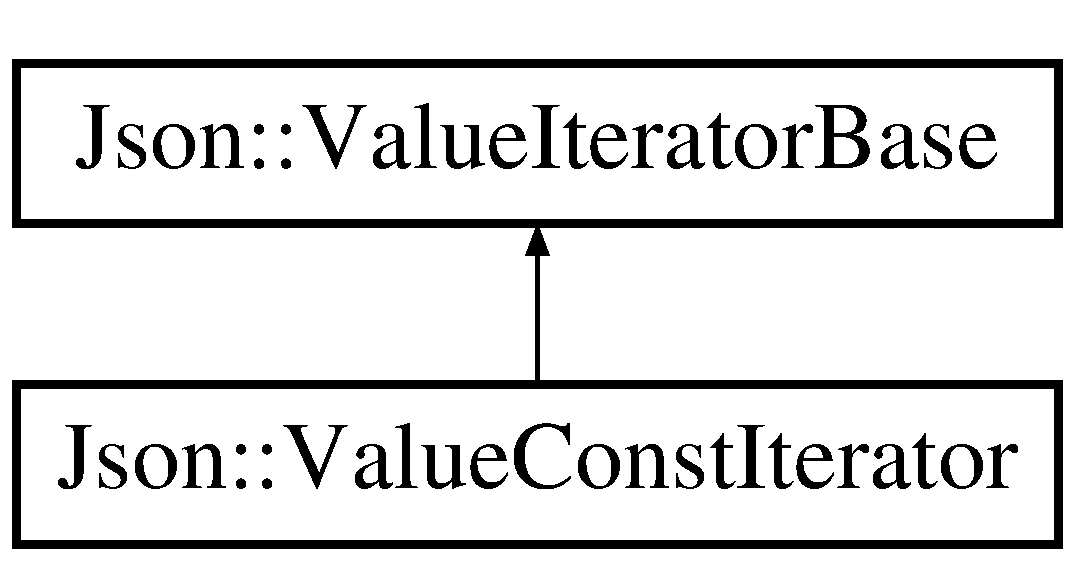
\includegraphics[height=2.000000cm]{classJson_1_1ValueConstIterator}
\end{center}
\end{figure}
\subsection*{Public Types}
\begin{DoxyCompactItemize}
\item 
\mbox{\Hypertarget{classJson_1_1ValueConstIterator_aa5f1707dcef4bfe73e23ddc14dbe760d}\label{classJson_1_1ValueConstIterator_aa5f1707dcef4bfe73e23ddc14dbe760d}} 
typedef const \hyperlink{classJson_1_1Value}{Value} {\bfseries value\+\_\+type}
\item 
\mbox{\Hypertarget{classJson_1_1ValueConstIterator_aa9b05c6a37cd352ea1ee6e13b816f709}\label{classJson_1_1ValueConstIterator_aa9b05c6a37cd352ea1ee6e13b816f709}} 
typedef const \hyperlink{classJson_1_1Value}{Value} \& {\bfseries reference}
\item 
\mbox{\Hypertarget{classJson_1_1ValueConstIterator_a400136bd8bc09e9fddec0785fa2cff14}\label{classJson_1_1ValueConstIterator_a400136bd8bc09e9fddec0785fa2cff14}} 
typedef const \hyperlink{classJson_1_1Value}{Value} $\ast$ {\bfseries pointer}
\item 
\mbox{\Hypertarget{classJson_1_1ValueConstIterator_a0c2e33e7eb5a80dd8709fb28ece83933}\label{classJson_1_1ValueConstIterator_a0c2e33e7eb5a80dd8709fb28ece83933}} 
typedef \hyperlink{classJson_1_1ValueConstIterator}{Value\+Const\+Iterator} {\bfseries Self\+Type}
\end{DoxyCompactItemize}
\subsection*{Public Member Functions}
\begin{DoxyCompactItemize}
\item 
\mbox{\Hypertarget{classJson_1_1ValueConstIterator_a7ef3df204a9ae83a0d8a3cd128e05c70}\label{classJson_1_1ValueConstIterator_a7ef3df204a9ae83a0d8a3cd128e05c70}} 
{\bfseries Value\+Const\+Iterator} (\hyperlink{classJson_1_1ValueIterator}{Value\+Iterator} const \&other)
\item 
\mbox{\Hypertarget{classJson_1_1ValueConstIterator_ad1b1c11f8d7fb22d4d3c231915f2b15b}\label{classJson_1_1ValueConstIterator_ad1b1c11f8d7fb22d4d3c231915f2b15b}} 
\hyperlink{classJson_1_1ValueIteratorBase}{Self\+Type} \& {\bfseries operator=} (const \hyperlink{classJson_1_1ValueIteratorBase}{Value\+Iterator\+Base} \&other)
\item 
\mbox{\Hypertarget{classJson_1_1ValueConstIterator_ab3f0c2edbfc8f7d60645f3d597d05e28}\label{classJson_1_1ValueConstIterator_ab3f0c2edbfc8f7d60645f3d597d05e28}} 
\hyperlink{classJson_1_1ValueIteratorBase}{Self\+Type} {\bfseries operator++} (int)
\item 
\mbox{\Hypertarget{classJson_1_1ValueConstIterator_a94935961e9331c6f7b907b05ec8df75e}\label{classJson_1_1ValueConstIterator_a94935961e9331c6f7b907b05ec8df75e}} 
\hyperlink{classJson_1_1ValueIteratorBase}{Self\+Type} {\bfseries operator-\/-\/} (int)
\item 
\mbox{\Hypertarget{classJson_1_1ValueConstIterator_a31415e44e44e56fb2bfda7e8bb784646}\label{classJson_1_1ValueConstIterator_a31415e44e44e56fb2bfda7e8bb784646}} 
\hyperlink{classJson_1_1ValueIteratorBase}{Self\+Type} \& {\bfseries operator-\/-\/} ()
\item 
\mbox{\Hypertarget{classJson_1_1ValueConstIterator_a2cfe2f7a94a688186efdafb1b181c319}\label{classJson_1_1ValueConstIterator_a2cfe2f7a94a688186efdafb1b181c319}} 
\hyperlink{classJson_1_1ValueIteratorBase}{Self\+Type} \& {\bfseries operator++} ()
\item 
\mbox{\Hypertarget{classJson_1_1ValueConstIterator_ae5612dad47a6387eef71d584fb741d0c}\label{classJson_1_1ValueConstIterator_ae5612dad47a6387eef71d584fb741d0c}} 
\hyperlink{classJson_1_1Value}{reference} {\bfseries operator$\ast$} () const
\item 
\mbox{\Hypertarget{classJson_1_1ValueConstIterator_a3c608ae53c192ee846eb265bae1cfeec}\label{classJson_1_1ValueConstIterator_a3c608ae53c192ee846eb265bae1cfeec}} 
\hyperlink{classJson_1_1Value}{pointer} {\bfseries operator-\/$>$} () const
\end{DoxyCompactItemize}
\subsection*{Friends}
\begin{DoxyCompactItemize}
\item 
\mbox{\Hypertarget{classJson_1_1ValueConstIterator_aeceedf6e1a7d48a588516ce2b1983d6f}\label{classJson_1_1ValueConstIterator_aeceedf6e1a7d48a588516ce2b1983d6f}} 
class {\bfseries Value}
\end{DoxyCompactItemize}
\subsection*{Additional Inherited Members}


\subsection{Detailed Description}
const iterator for object and array value. 



The documentation for this class was generated from the following files\+:\begin{DoxyCompactItemize}
\item 
json/json.\+h\item 
jsoncpp.\+cpp\end{DoxyCompactItemize}

\hypertarget{unionJson_1_1Value_1_1ValueHolder}{}\section{Json\+:\+:Value\+:\+:Value\+Holder Union Reference}
\label{unionJson_1_1Value_1_1ValueHolder}\index{Json\+::\+Value\+::\+Value\+Holder@{Json\+::\+Value\+::\+Value\+Holder}}
\subsection*{Public Attributes}
\begin{DoxyCompactItemize}
\item 
\hyperlink{classJson_1_1Value_a1cbb82642ed05109b9833e49f042ece7_a1cbb82642ed05109b9833e49f042ece7}{Largest\+Int} \hyperlink{unionJson_1_1Value_1_1ValueHolder_adbfb384301298844ed955ba5cf6015a0_adbfb384301298844ed955ba5cf6015a0}{int\+\_\+}
\item 
\hyperlink{classJson_1_1Value_a6682a3684d635e03fc06ba229fa24eec_a6682a3684d635e03fc06ba229fa24eec}{Largest\+U\+Int} \hyperlink{unionJson_1_1Value_1_1ValueHolder_aab65665dc15a24a29a8e93cdeeaa7e50_aab65665dc15a24a29a8e93cdeeaa7e50}{uint\+\_\+}
\item 
double \hyperlink{unionJson_1_1Value_1_1ValueHolder_af0c5ca724e5fe3a15db773d750e2351e_af0c5ca724e5fe3a15db773d750e2351e}{real\+\_\+}
\item 
bool \hyperlink{unionJson_1_1Value_1_1ValueHolder_a92edab1861dadbfefd8be5fd4285eefe_a92edab1861dadbfefd8be5fd4285eefe}{bool\+\_\+}
\item 
char $\ast$ \hyperlink{unionJson_1_1Value_1_1ValueHolder_a70ac2b153bc405527baa3850d2ddc3cb_a70ac2b153bc405527baa3850d2ddc3cb}{string\+\_\+}
\item 
\hyperlink{classJson_1_1Value_a08b6c80c3af7071d908dabf044de5388_a08b6c80c3af7071d908dabf044de5388}{Object\+Values} $\ast$ \hyperlink{unionJson_1_1Value_1_1ValueHolder_a1e7a5b86d4f52234f55c847ad1ce389a_a1e7a5b86d4f52234f55c847ad1ce389a}{map\+\_\+}
\end{DoxyCompactItemize}


\subsection{Member Data Documentation}
\mbox{\Hypertarget{unionJson_1_1Value_1_1ValueHolder_a92edab1861dadbfefd8be5fd4285eefe_a92edab1861dadbfefd8be5fd4285eefe}\label{unionJson_1_1Value_1_1ValueHolder_a92edab1861dadbfefd8be5fd4285eefe_a92edab1861dadbfefd8be5fd4285eefe}} 
\index{Json\+::\+Value\+::\+Value\+Holder@{Json\+::\+Value\+::\+Value\+Holder}!bool\+\_\+@{bool\+\_\+}}
\index{bool\+\_\+@{bool\+\_\+}!Json\+::\+Value\+::\+Value\+Holder@{Json\+::\+Value\+::\+Value\+Holder}}
\subsubsection{\texorpdfstring{bool\+\_\+}{bool\_}}
{\footnotesize\ttfamily bool Json\+::\+Value\+::\+Value\+Holder\+::bool\+\_\+}



Referenced by Json\+::\+Value\+::as\+Bool(), Json\+::\+Value\+::as\+Double(), Json\+::\+Value\+::as\+Float(), Json\+::\+Value\+::as\+Int(), Json\+::\+Value\+::as\+Int64(), Json\+::\+Value\+::as\+String(), Json\+::\+Value\+::as\+U\+Int(), Json\+::\+Value\+::as\+U\+Int64(), Json\+::\+Value\+::is\+Convertible\+To(), Json\+::\+Value\+::operator$<$(), Json\+::\+Value\+::operator==(), and Json\+::\+Value\+::\+Value().

\mbox{\Hypertarget{unionJson_1_1Value_1_1ValueHolder_adbfb384301298844ed955ba5cf6015a0_adbfb384301298844ed955ba5cf6015a0}\label{unionJson_1_1Value_1_1ValueHolder_adbfb384301298844ed955ba5cf6015a0_adbfb384301298844ed955ba5cf6015a0}} 
\index{Json\+::\+Value\+::\+Value\+Holder@{Json\+::\+Value\+::\+Value\+Holder}!int\+\_\+@{int\+\_\+}}
\index{int\+\_\+@{int\+\_\+}!Json\+::\+Value\+::\+Value\+Holder@{Json\+::\+Value\+::\+Value\+Holder}}
\subsubsection{\texorpdfstring{int\+\_\+}{int\_}}
{\footnotesize\ttfamily \hyperlink{classJson_1_1Value_a1cbb82642ed05109b9833e49f042ece7_a1cbb82642ed05109b9833e49f042ece7}{Largest\+Int} Json\+::\+Value\+::\+Value\+Holder\+::int\+\_\+}



Referenced by Json\+::\+Value\+::as\+Bool(), Json\+::\+Value\+::as\+Double(), Json\+::\+Value\+::as\+Float(), Json\+::\+Value\+::as\+Int(), Json\+::\+Value\+::as\+Int64(), Json\+::\+Value\+::as\+String(), Json\+::\+Value\+::as\+U\+Int(), Json\+::\+Value\+::as\+U\+Int64(), Json\+::\+Value\+::is\+Int(), Json\+::\+Value\+::is\+U\+Int(), Json\+::\+Value\+::is\+U\+Int64(), Json\+::\+Value\+::operator$<$(), Json\+::\+Value\+::operator==(), and Json\+::\+Value\+::\+Value().

\mbox{\Hypertarget{unionJson_1_1Value_1_1ValueHolder_a1e7a5b86d4f52234f55c847ad1ce389a_a1e7a5b86d4f52234f55c847ad1ce389a}\label{unionJson_1_1Value_1_1ValueHolder_a1e7a5b86d4f52234f55c847ad1ce389a_a1e7a5b86d4f52234f55c847ad1ce389a}} 
\index{Json\+::\+Value\+::\+Value\+Holder@{Json\+::\+Value\+::\+Value\+Holder}!map\+\_\+@{map\+\_\+}}
\index{map\+\_\+@{map\+\_\+}!Json\+::\+Value\+::\+Value\+Holder@{Json\+::\+Value\+::\+Value\+Holder}}
\subsubsection{\texorpdfstring{map\+\_\+}{map\_}}
{\footnotesize\ttfamily \hyperlink{classJson_1_1Value_a08b6c80c3af7071d908dabf044de5388_a08b6c80c3af7071d908dabf044de5388}{Object\+Values}$\ast$ Json\+::\+Value\+::\+Value\+Holder\+::map\+\_\+}



Referenced by Json\+::\+Value\+::begin(), Json\+::\+Value\+::clear(), Json\+::\+Value\+::end(), Json\+::\+Value\+::find(), Json\+::\+Value\+::get\+Member\+Names(), Json\+::\+Value\+::is\+Convertible\+To(), Json\+::\+Value\+::operator$<$(), Json\+::\+Value\+::operator==(), Json\+::\+Value\+::operator\mbox{[}$\,$\mbox{]}(), Json\+::\+Value\+::remove\+Index(), Json\+::\+Value\+::remove\+Member(), Json\+::\+Value\+::resize(), Json\+::\+Value\+::resolve\+Reference(), Json\+::\+Value\+::size(), Json\+::\+Value\+::\+Value(), and Json\+::\+Value\+::$\sim$\+Value().

\mbox{\Hypertarget{unionJson_1_1Value_1_1ValueHolder_af0c5ca724e5fe3a15db773d750e2351e_af0c5ca724e5fe3a15db773d750e2351e}\label{unionJson_1_1Value_1_1ValueHolder_af0c5ca724e5fe3a15db773d750e2351e_af0c5ca724e5fe3a15db773d750e2351e}} 
\index{Json\+::\+Value\+::\+Value\+Holder@{Json\+::\+Value\+::\+Value\+Holder}!real\+\_\+@{real\+\_\+}}
\index{real\+\_\+@{real\+\_\+}!Json\+::\+Value\+::\+Value\+Holder@{Json\+::\+Value\+::\+Value\+Holder}}
\subsubsection{\texorpdfstring{real\+\_\+}{real\_}}
{\footnotesize\ttfamily double Json\+::\+Value\+::\+Value\+Holder\+::real\+\_\+}



Referenced by Json\+::\+Value\+::as\+Bool(), Json\+::\+Value\+::as\+Double(), Json\+::\+Value\+::as\+Float(), Json\+::\+Value\+::as\+Int(), Json\+::\+Value\+::as\+Int64(), Json\+::\+Value\+::as\+String(), Json\+::\+Value\+::as\+U\+Int(), Json\+::\+Value\+::as\+U\+Int64(), Json\+::\+Value\+::is\+Convertible\+To(), Json\+::\+Value\+::is\+Int(), Json\+::\+Value\+::is\+Int64(), Json\+::\+Value\+::is\+Integral(), Json\+::\+Value\+::is\+U\+Int(), Json\+::\+Value\+::is\+U\+Int64(), Json\+::\+Value\+::operator$<$(), Json\+::\+Value\+::operator==(), and Json\+::\+Value\+::\+Value().

\mbox{\Hypertarget{unionJson_1_1Value_1_1ValueHolder_a70ac2b153bc405527baa3850d2ddc3cb_a70ac2b153bc405527baa3850d2ddc3cb}\label{unionJson_1_1Value_1_1ValueHolder_a70ac2b153bc405527baa3850d2ddc3cb_a70ac2b153bc405527baa3850d2ddc3cb}} 
\index{Json\+::\+Value\+::\+Value\+Holder@{Json\+::\+Value\+::\+Value\+Holder}!string\+\_\+@{string\+\_\+}}
\index{string\+\_\+@{string\+\_\+}!Json\+::\+Value\+::\+Value\+Holder@{Json\+::\+Value\+::\+Value\+Holder}}
\subsubsection{\texorpdfstring{string\+\_\+}{string\_}}
{\footnotesize\ttfamily char$\ast$ Json\+::\+Value\+::\+Value\+Holder\+::string\+\_\+}



Referenced by Json\+::\+Value\+::as\+C\+String(), Json\+::\+Value\+::as\+String(), Json\+::\+Value\+::get\+String(), Json\+::\+Value\+::operator$<$(), Json\+::\+Value\+::operator==(), Json\+::\+Value\+::\+Value(), and Json\+::\+Value\+::$\sim$\+Value().

\mbox{\Hypertarget{unionJson_1_1Value_1_1ValueHolder_aab65665dc15a24a29a8e93cdeeaa7e50_aab65665dc15a24a29a8e93cdeeaa7e50}\label{unionJson_1_1Value_1_1ValueHolder_aab65665dc15a24a29a8e93cdeeaa7e50_aab65665dc15a24a29a8e93cdeeaa7e50}} 
\index{Json\+::\+Value\+::\+Value\+Holder@{Json\+::\+Value\+::\+Value\+Holder}!uint\+\_\+@{uint\+\_\+}}
\index{uint\+\_\+@{uint\+\_\+}!Json\+::\+Value\+::\+Value\+Holder@{Json\+::\+Value\+::\+Value\+Holder}}
\subsubsection{\texorpdfstring{uint\+\_\+}{uint\_}}
{\footnotesize\ttfamily \hyperlink{classJson_1_1Value_a6682a3684d635e03fc06ba229fa24eec_a6682a3684d635e03fc06ba229fa24eec}{Largest\+U\+Int} Json\+::\+Value\+::\+Value\+Holder\+::uint\+\_\+}



Referenced by Json\+::\+Value\+::as\+Bool(), Json\+::\+Value\+::as\+Double(), Json\+::\+Value\+::as\+Float(), Json\+::\+Value\+::as\+Int(), Json\+::\+Value\+::as\+Int64(), Json\+::\+Value\+::as\+String(), Json\+::\+Value\+::as\+U\+Int(), Json\+::\+Value\+::as\+U\+Int64(), Json\+::\+Value\+::is\+Int(), Json\+::\+Value\+::is\+Int64(), Json\+::\+Value\+::is\+U\+Int(), Json\+::\+Value\+::operator$<$(), Json\+::\+Value\+::operator==(), Json\+::\+Value\+::\+Value(), and Json\+::\+Value\+::$\sim$\+Value().



The documentation for this union was generated from the following file\+:\begin{DoxyCompactItemize}
\item 
json/\hyperlink{json_8h}{json.\+h}\end{DoxyCompactItemize}

\hypertarget{classJson_1_1ValueIterator}{}\section{Json\+:\+:Value\+Iterator Class Reference}
\label{classJson_1_1ValueIterator}\index{Json\+::\+Value\+Iterator@{Json\+::\+Value\+Iterator}}


Iterator for object and array value.  




{\ttfamily \#include $<$json.\+h$>$}

Inheritance diagram for Json\+:\+:Value\+Iterator\+:\begin{figure}[H]
\begin{center}
\leavevmode
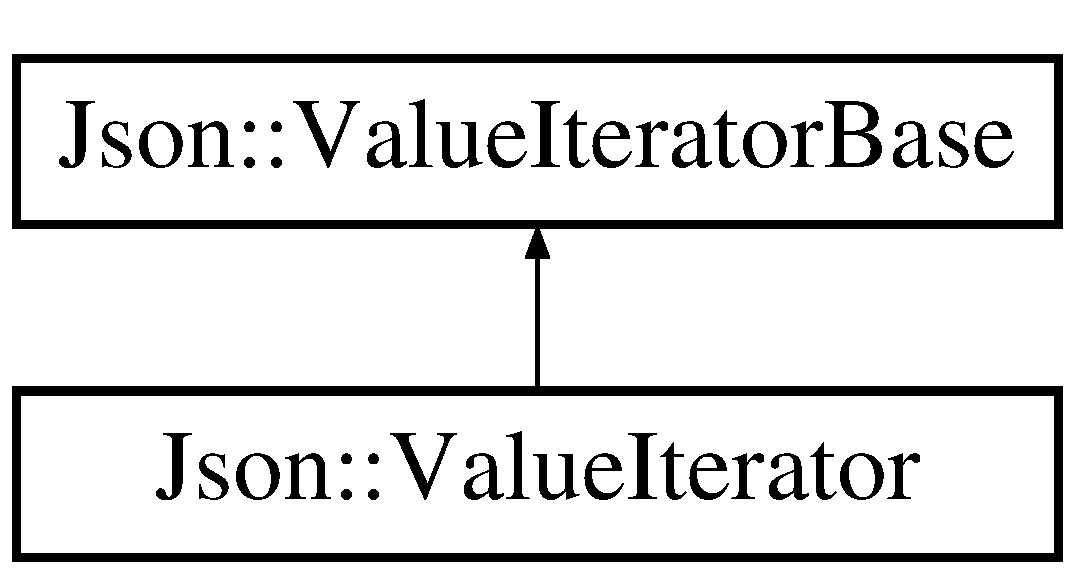
\includegraphics[height=2.000000cm]{classJson_1_1ValueIterator}
\end{center}
\end{figure}
\subsection*{Public Types}
\begin{DoxyCompactItemize}
\item 
\mbox{\Hypertarget{classJson_1_1ValueIterator_a2c5ba7be611f05546530c8a88b2d2e37}\label{classJson_1_1ValueIterator_a2c5ba7be611f05546530c8a88b2d2e37}} 
typedef \hyperlink{classJson_1_1Value}{Value} {\bfseries value\+\_\+type}
\item 
\mbox{\Hypertarget{classJson_1_1ValueIterator_a308b8932ffc83eaa9d12dadd5c11a7dd}\label{classJson_1_1ValueIterator_a308b8932ffc83eaa9d12dadd5c11a7dd}} 
typedef unsigned int {\bfseries size\+\_\+t}
\item 
\mbox{\Hypertarget{classJson_1_1ValueIterator_a2be1a9aa60bbfc8812e9dd1a7f1a8786}\label{classJson_1_1ValueIterator_a2be1a9aa60bbfc8812e9dd1a7f1a8786}} 
typedef int {\bfseries difference\+\_\+type}
\item 
\mbox{\Hypertarget{classJson_1_1ValueIterator_ae87929b4567aa00372cf602c43b57160}\label{classJson_1_1ValueIterator_ae87929b4567aa00372cf602c43b57160}} 
typedef \hyperlink{classJson_1_1Value}{Value} \& {\bfseries reference}
\item 
\mbox{\Hypertarget{classJson_1_1ValueIterator_acec45feb1ef1f3bf81240157d06d5432}\label{classJson_1_1ValueIterator_acec45feb1ef1f3bf81240157d06d5432}} 
typedef \hyperlink{classJson_1_1Value}{Value} $\ast$ {\bfseries pointer}
\item 
\mbox{\Hypertarget{classJson_1_1ValueIterator_a23357670fdad61792670d86f62db7e16}\label{classJson_1_1ValueIterator_a23357670fdad61792670d86f62db7e16}} 
typedef \hyperlink{classJson_1_1ValueIterator}{Value\+Iterator} {\bfseries Self\+Type}
\end{DoxyCompactItemize}
\subsection*{Public Member Functions}
\begin{DoxyCompactItemize}
\item 
\mbox{\Hypertarget{classJson_1_1ValueIterator_aa85aa208670891670392259efa0143bb}\label{classJson_1_1ValueIterator_aa85aa208670891670392259efa0143bb}} 
{\bfseries Value\+Iterator} (const \hyperlink{classJson_1_1ValueConstIterator}{Value\+Const\+Iterator} \&other)
\item 
\mbox{\Hypertarget{classJson_1_1ValueIterator_a7d5e58a9a4a553968acdf3064b39d21c}\label{classJson_1_1ValueIterator_a7d5e58a9a4a553968acdf3064b39d21c}} 
{\bfseries Value\+Iterator} (const \hyperlink{classJson_1_1ValueIterator}{Value\+Iterator} \&other)
\item 
\mbox{\Hypertarget{classJson_1_1ValueIterator_a8e23312b1db874f7e403fd7e76611bdc}\label{classJson_1_1ValueIterator_a8e23312b1db874f7e403fd7e76611bdc}} 
\hyperlink{classJson_1_1ValueIteratorBase}{Self\+Type} \& {\bfseries operator=} (const \hyperlink{classJson_1_1ValueIteratorBase}{Self\+Type} \&other)
\item 
\mbox{\Hypertarget{classJson_1_1ValueIterator_abcf4ddd994a010742cd4a436d65acd08}\label{classJson_1_1ValueIterator_abcf4ddd994a010742cd4a436d65acd08}} 
\hyperlink{classJson_1_1ValueIteratorBase}{Self\+Type} {\bfseries operator++} (int)
\item 
\mbox{\Hypertarget{classJson_1_1ValueIterator_a06d6a29d96caf6af324a53973159e12b}\label{classJson_1_1ValueIterator_a06d6a29d96caf6af324a53973159e12b}} 
\hyperlink{classJson_1_1ValueIteratorBase}{Self\+Type} {\bfseries operator-\/-\/} (int)
\item 
\mbox{\Hypertarget{classJson_1_1ValueIterator_a811302a868518a0995a9def955df5720}\label{classJson_1_1ValueIterator_a811302a868518a0995a9def955df5720}} 
\hyperlink{classJson_1_1ValueIteratorBase}{Self\+Type} \& {\bfseries operator-\/-\/} ()
\item 
\mbox{\Hypertarget{classJson_1_1ValueIterator_a92146c46f8249e2b2d12869e70cd4cee}\label{classJson_1_1ValueIterator_a92146c46f8249e2b2d12869e70cd4cee}} 
\hyperlink{classJson_1_1ValueIteratorBase}{Self\+Type} \& {\bfseries operator++} ()
\item 
\mbox{\Hypertarget{classJson_1_1ValueIterator_a3be48b0c1729ec2532f1ff27ad465d32}\label{classJson_1_1ValueIterator_a3be48b0c1729ec2532f1ff27ad465d32}} 
\hyperlink{classJson_1_1Value}{reference} {\bfseries operator$\ast$} () const
\item 
\mbox{\Hypertarget{classJson_1_1ValueIterator_a8dfc1603f92467591d524d0326f35534}\label{classJson_1_1ValueIterator_a8dfc1603f92467591d524d0326f35534}} 
\hyperlink{classJson_1_1Value}{pointer} {\bfseries operator-\/$>$} () const
\end{DoxyCompactItemize}
\subsection*{Friends}
\begin{DoxyCompactItemize}
\item 
\mbox{\Hypertarget{classJson_1_1ValueIterator_aeceedf6e1a7d48a588516ce2b1983d6f}\label{classJson_1_1ValueIterator_aeceedf6e1a7d48a588516ce2b1983d6f}} 
class {\bfseries Value}
\end{DoxyCompactItemize}
\subsection*{Additional Inherited Members}


\subsection{Detailed Description}
Iterator for object and array value. 

The documentation for this class was generated from the following files\+:\begin{DoxyCompactItemize}
\item 
json/json.\+h\item 
jsoncpp.\+cpp\end{DoxyCompactItemize}

\hypertarget{classJson_1_1ValueIteratorBase}{}\section{Json\+:\+:Value\+Iterator\+Base Class Reference}
\label{classJson_1_1ValueIteratorBase}\index{Json\+::\+Value\+Iterator\+Base@{Json\+::\+Value\+Iterator\+Base}}


base class for \hyperlink{classJson_1_1Value}{Value} iterators.  




{\ttfamily \#include $<$json.\+h$>$}

Inheritance diagram for Json\+:\+:Value\+Iterator\+Base\+:\begin{figure}[H]
\begin{center}
\leavevmode
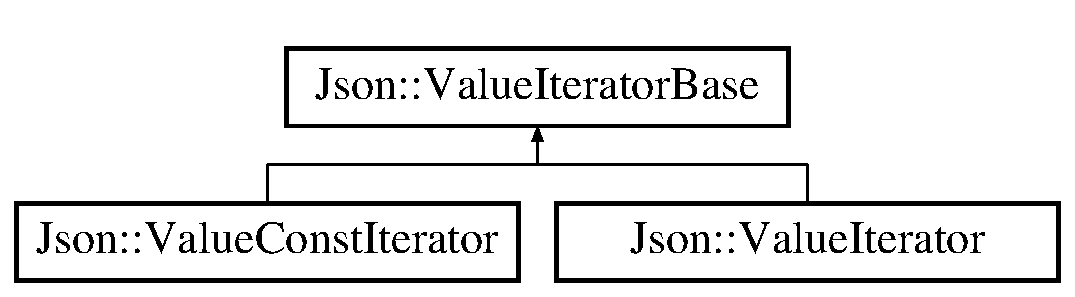
\includegraphics[height=2.000000cm]{classJson_1_1ValueIteratorBase}
\end{center}
\end{figure}
\subsection*{Public Types}
\begin{DoxyCompactItemize}
\item 
\mbox{\Hypertarget{classJson_1_1ValueIteratorBase_a02fd11a4fbdc0007da1e8bcf5e6b83c3}\label{classJson_1_1ValueIteratorBase_a02fd11a4fbdc0007da1e8bcf5e6b83c3}} 
typedef std\+::bidirectional\+\_\+iterator\+\_\+tag {\bfseries iterator\+\_\+category}
\item 
\mbox{\Hypertarget{classJson_1_1ValueIteratorBase_a9d3a3c7ce5cdefe23cb486239cf07bb5}\label{classJson_1_1ValueIteratorBase_a9d3a3c7ce5cdefe23cb486239cf07bb5}} 
typedef unsigned int {\bfseries size\+\_\+t}
\item 
\mbox{\Hypertarget{classJson_1_1ValueIteratorBase_a4e44bf8cbd17ec8d6e2c185904a15ebd}\label{classJson_1_1ValueIteratorBase_a4e44bf8cbd17ec8d6e2c185904a15ebd}} 
typedef int {\bfseries difference\+\_\+type}
\item 
\mbox{\Hypertarget{classJson_1_1ValueIteratorBase_a9d2a940d03ea06d20d972f41a89149ee}\label{classJson_1_1ValueIteratorBase_a9d2a940d03ea06d20d972f41a89149ee}} 
typedef \hyperlink{classJson_1_1ValueIteratorBase}{Value\+Iterator\+Base} {\bfseries Self\+Type}
\end{DoxyCompactItemize}
\subsection*{Public Member Functions}
\begin{DoxyCompactItemize}
\item 
\mbox{\Hypertarget{classJson_1_1ValueIteratorBase_a1248d8016f88b51371a0fcbd355b3cfd}\label{classJson_1_1ValueIteratorBase_a1248d8016f88b51371a0fcbd355b3cfd}} 
bool {\bfseries operator==} (const \hyperlink{classJson_1_1ValueIteratorBase}{Self\+Type} \&other) const
\item 
\mbox{\Hypertarget{classJson_1_1ValueIteratorBase_aa83bdcc8114b7d040eb8eb42eeed5f4a}\label{classJson_1_1ValueIteratorBase_aa83bdcc8114b7d040eb8eb42eeed5f4a}} 
bool {\bfseries operator!=} (const \hyperlink{classJson_1_1ValueIteratorBase}{Self\+Type} \&other) const
\item 
\mbox{\Hypertarget{classJson_1_1ValueIteratorBase_a98e254263fca5f1fc8fcac7bcb0260bf}\label{classJson_1_1ValueIteratorBase_a98e254263fca5f1fc8fcac7bcb0260bf}} 
difference\+\_\+type {\bfseries operator-\/} (const \hyperlink{classJson_1_1ValueIteratorBase}{Self\+Type} \&other) const
\item 
\hyperlink{classJson_1_1Value}{Value} \hyperlink{classJson_1_1ValueIteratorBase_a3838ba39c43c518cf3ed4aa6ce78ccad}{key} () const
\item 
\mbox{\Hypertarget{classJson_1_1ValueIteratorBase_a549c66a0bd20e9ae772175a5c0d2e88a}\label{classJson_1_1ValueIteratorBase_a549c66a0bd20e9ae772175a5c0d2e88a}} 
U\+Int \hyperlink{classJson_1_1ValueIteratorBase_a549c66a0bd20e9ae772175a5c0d2e88a}{index} () const
\begin{DoxyCompactList}\small\item\em Return the index of the referenced \hyperlink{classJson_1_1Value}{Value}, or -\/1 if it is not an array\+Value. \end{DoxyCompactList}\item 
J\+S\+O\+N\+C\+P\+P\+\_\+\+S\+T\+R\+I\+NG \hyperlink{classJson_1_1ValueIteratorBase_a522989403c976fdbb94da846b99418db}{name} () const
\item 
char const  $\ast$ \hyperlink{classJson_1_1ValueIteratorBase_a54765da6759fd3f1edcbfbaf308ec263}{member\+Name} () const
\item 
char const  $\ast$ \hyperlink{classJson_1_1ValueIteratorBase_a391c9cbd0edf9a447b37df00e8ce6059}{member\+Name} (char const $\ast$$\ast$end) const
\item 
\mbox{\Hypertarget{classJson_1_1ValueIteratorBase_a640e990e5f03a96fd650122a2906f59d}\label{classJson_1_1ValueIteratorBase_a640e990e5f03a96fd650122a2906f59d}} 
{\bfseries Value\+Iterator\+Base} (const Value\+::\+Object\+Values\+::iterator \&current)
\end{DoxyCompactItemize}
\subsection*{Protected Member Functions}
\begin{DoxyCompactItemize}
\item 
\mbox{\Hypertarget{classJson_1_1ValueIteratorBase_aa5b75c9514a30ba2ea3c9a35c165c18e}\label{classJson_1_1ValueIteratorBase_aa5b75c9514a30ba2ea3c9a35c165c18e}} 
\hyperlink{classJson_1_1Value}{Value} \& {\bfseries deref} () const
\item 
\mbox{\Hypertarget{classJson_1_1ValueIteratorBase_afe58f9534e1fd2033419fd9fe244551e}\label{classJson_1_1ValueIteratorBase_afe58f9534e1fd2033419fd9fe244551e}} 
void {\bfseries increment} ()
\item 
\mbox{\Hypertarget{classJson_1_1ValueIteratorBase_affc8cf5ff54a9f432cc693362c153fa6}\label{classJson_1_1ValueIteratorBase_affc8cf5ff54a9f432cc693362c153fa6}} 
void {\bfseries decrement} ()
\item 
\mbox{\Hypertarget{classJson_1_1ValueIteratorBase_af11473c9e20d07782e42b52a2f9e4540}\label{classJson_1_1ValueIteratorBase_af11473c9e20d07782e42b52a2f9e4540}} 
difference\+\_\+type {\bfseries compute\+Distance} (const \hyperlink{classJson_1_1ValueIteratorBase}{Self\+Type} \&other) const
\item 
\mbox{\Hypertarget{classJson_1_1ValueIteratorBase_a010b5ad3f3337ae3732e5d7e16ca5e25}\label{classJson_1_1ValueIteratorBase_a010b5ad3f3337ae3732e5d7e16ca5e25}} 
bool {\bfseries is\+Equal} (const \hyperlink{classJson_1_1ValueIteratorBase}{Self\+Type} \&other) const
\item 
\mbox{\Hypertarget{classJson_1_1ValueIteratorBase_a496e6aba44808433ec5858c178be5719}\label{classJson_1_1ValueIteratorBase_a496e6aba44808433ec5858c178be5719}} 
void {\bfseries copy} (const \hyperlink{classJson_1_1ValueIteratorBase}{Self\+Type} \&other)
\end{DoxyCompactItemize}


\subsection{Detailed Description}
base class for \hyperlink{classJson_1_1Value}{Value} iterators. 



\subsection{Member Function Documentation}
\mbox{\Hypertarget{classJson_1_1ValueIteratorBase_a3838ba39c43c518cf3ed4aa6ce78ccad}\label{classJson_1_1ValueIteratorBase_a3838ba39c43c518cf3ed4aa6ce78ccad}} 
\index{Json\+::\+Value\+Iterator\+Base@{Json\+::\+Value\+Iterator\+Base}!key@{key}}
\index{key@{key}!Json\+::\+Value\+Iterator\+Base@{Json\+::\+Value\+Iterator\+Base}}
\subsubsection{\texorpdfstring{key()}{key()}}
{\footnotesize\ttfamily \hyperlink{classJson_1_1Value}{Value} Json\+::\+Value\+Iterator\+Base\+::key (\begin{DoxyParamCaption}{ }\end{DoxyParamCaption}) const}

Return either the index or the member name of the referenced value as a \hyperlink{classJson_1_1Value}{Value}. \mbox{\Hypertarget{classJson_1_1ValueIteratorBase_a54765da6759fd3f1edcbfbaf308ec263}\label{classJson_1_1ValueIteratorBase_a54765da6759fd3f1edcbfbaf308ec263}} 
\index{Json\+::\+Value\+Iterator\+Base@{Json\+::\+Value\+Iterator\+Base}!member\+Name@{member\+Name}}
\index{member\+Name@{member\+Name}!Json\+::\+Value\+Iterator\+Base@{Json\+::\+Value\+Iterator\+Base}}
\subsubsection{\texorpdfstring{member\+Name()}{memberName()}\hspace{0.1cm}{\footnotesize\ttfamily [1/2]}}
{\footnotesize\ttfamily char const  $\ast$ Json\+::\+Value\+Iterator\+Base\+::member\+Name (\begin{DoxyParamCaption}{ }\end{DoxyParamCaption}) const}

Return the member name of the referenced \hyperlink{classJson_1_1Value}{Value}. \char`\"{}\char`\"{} if it is not an object\+Value. \begin{DoxyRefDesc}{Deprecated}
\item[\hyperlink{deprecated__deprecated000004}{Deprecated}]This cannot be used for U\+T\+F-\/8 strings, since there can be embedded nulls. \end{DoxyRefDesc}
\mbox{\Hypertarget{classJson_1_1ValueIteratorBase_a391c9cbd0edf9a447b37df00e8ce6059}\label{classJson_1_1ValueIteratorBase_a391c9cbd0edf9a447b37df00e8ce6059}} 
\index{Json\+::\+Value\+Iterator\+Base@{Json\+::\+Value\+Iterator\+Base}!member\+Name@{member\+Name}}
\index{member\+Name@{member\+Name}!Json\+::\+Value\+Iterator\+Base@{Json\+::\+Value\+Iterator\+Base}}
\subsubsection{\texorpdfstring{member\+Name()}{memberName()}\hspace{0.1cm}{\footnotesize\ttfamily [2/2]}}
{\footnotesize\ttfamily char const  $\ast$ Json\+::\+Value\+Iterator\+Base\+::member\+Name (\begin{DoxyParamCaption}\item[{char const $\ast$$\ast$}]{end }\end{DoxyParamCaption}) const}

Return the member name of the referenced \hyperlink{classJson_1_1Value}{Value}, or N\+U\+LL if it is not an object\+Value. \begin{DoxyNote}{Note}
Better version than \hyperlink{classJson_1_1ValueIteratorBase_a54765da6759fd3f1edcbfbaf308ec263}{member\+Name()}. Allows embedded nulls. 
\end{DoxyNote}
\mbox{\Hypertarget{classJson_1_1ValueIteratorBase_a522989403c976fdbb94da846b99418db}\label{classJson_1_1ValueIteratorBase_a522989403c976fdbb94da846b99418db}} 
\index{Json\+::\+Value\+Iterator\+Base@{Json\+::\+Value\+Iterator\+Base}!name@{name}}
\index{name@{name}!Json\+::\+Value\+Iterator\+Base@{Json\+::\+Value\+Iterator\+Base}}
\subsubsection{\texorpdfstring{name()}{name()}}
{\footnotesize\ttfamily J\+S\+O\+N\+C\+P\+P\+\_\+\+S\+T\+R\+I\+NG Json\+::\+Value\+Iterator\+Base\+::name (\begin{DoxyParamCaption}{ }\end{DoxyParamCaption}) const}

Return the member name of the referenced \hyperlink{classJson_1_1Value}{Value}, or \char`\"{}\char`\"{} if it is not an object\+Value. \begin{DoxyNote}{Note}
Avoid {\ttfamily c\+\_\+str()} on result, as embedded zeroes are possible. 
\end{DoxyNote}


The documentation for this class was generated from the following files\+:\begin{DoxyCompactItemize}
\item 
json/json.\+h\item 
jsoncpp.\+cpp\end{DoxyCompactItemize}

\hypertarget{structwebsocket__message}{}\section{websocket\+\_\+message Struct Reference}
\label{structwebsocket__message}\index{websocket\+\_\+message@{websocket\+\_\+message}}
\subsection*{Public Attributes}
\begin{DoxyCompactItemize}
\item 
\mbox{\Hypertarget{structwebsocket__message_aeb8922c34831455b764d83083ae39968}\label{structwebsocket__message_aeb8922c34831455b764d83083ae39968}} 
unsigned char $\ast$ {\bfseries data}
\item 
\mbox{\Hypertarget{structwebsocket__message_af7ae89c0cba9566b64a47d40c5ea700a}\label{structwebsocket__message_af7ae89c0cba9566b64a47d40c5ea700a}} 
size\+\_\+t {\bfseries size}
\item 
\mbox{\Hypertarget{structwebsocket__message_a72b32c83b4a065faac7ae28802a5adf1}\label{structwebsocket__message_a72b32c83b4a065faac7ae28802a5adf1}} 
unsigned char {\bfseries flags}
\end{DoxyCompactItemize}


The documentation for this struct was generated from the following file\+:\begin{DoxyCompactItemize}
\item 
mongoose.\+h\end{DoxyCompactItemize}

\hypertarget{structws__mask__ctx}{}\section{ws\+\_\+mask\+\_\+ctx Struct Reference}
\label{structws__mask__ctx}\index{ws\+\_\+mask\+\_\+ctx@{ws\+\_\+mask\+\_\+ctx}}
\subsection*{Public Attributes}
\begin{DoxyCompactItemize}
\item 
size\+\_\+t \hyperlink{structws__mask__ctx_a475d1d7c7e1ffef41e9ddd94c738dc93_a475d1d7c7e1ffef41e9ddd94c738dc93}{pos}
\item 
uint32\+\_\+t \hyperlink{structws__mask__ctx_a5d0e6527780100ef7cac724b7b7c43ca_a5d0e6527780100ef7cac724b7b7c43ca}{mask}
\end{DoxyCompactItemize}


\subsection{Member Data Documentation}
\mbox{\Hypertarget{structws__mask__ctx_a5d0e6527780100ef7cac724b7b7c43ca_a5d0e6527780100ef7cac724b7b7c43ca}\label{structws__mask__ctx_a5d0e6527780100ef7cac724b7b7c43ca_a5d0e6527780100ef7cac724b7b7c43ca}} 
\index{ws\+\_\+mask\+\_\+ctx@{ws\+\_\+mask\+\_\+ctx}!mask@{mask}}
\index{mask@{mask}!ws\+\_\+mask\+\_\+ctx@{ws\+\_\+mask\+\_\+ctx}}
\subsubsection{\texorpdfstring{mask}{mask}}
{\footnotesize\ttfamily uint32\+\_\+t ws\+\_\+mask\+\_\+ctx\+::mask}



Referenced by mg\+\_\+send\+\_\+ws\+\_\+header(), and mg\+\_\+ws\+\_\+mask\+\_\+frame().

\mbox{\Hypertarget{structws__mask__ctx_a475d1d7c7e1ffef41e9ddd94c738dc93_a475d1d7c7e1ffef41e9ddd94c738dc93}\label{structws__mask__ctx_a475d1d7c7e1ffef41e9ddd94c738dc93_a475d1d7c7e1ffef41e9ddd94c738dc93}} 
\index{ws\+\_\+mask\+\_\+ctx@{ws\+\_\+mask\+\_\+ctx}!pos@{pos}}
\index{pos@{pos}!ws\+\_\+mask\+\_\+ctx@{ws\+\_\+mask\+\_\+ctx}}
\subsubsection{\texorpdfstring{pos}{pos}}
{\footnotesize\ttfamily size\+\_\+t ws\+\_\+mask\+\_\+ctx\+::pos}



Referenced by mg\+\_\+send\+\_\+ws\+\_\+header(), and mg\+\_\+ws\+\_\+mask\+\_\+frame().



The documentation for this struct was generated from the following file\+:\begin{DoxyCompactItemize}
\item 
\hyperlink{mongoose_8c}{mongoose.\+c}\end{DoxyCompactItemize}

\hypertarget{classTBT_1_1WSClientInterface}{}\section{T\+BT\+:\+:W\+S\+Client\+Interface Class Reference}
\label{classTBT_1_1WSClientInterface}\index{T\+B\+T\+::\+W\+S\+Client\+Interface@{T\+B\+T\+::\+W\+S\+Client\+Interface}}
Inheritance diagram for T\+BT\+:\+:W\+S\+Client\+Interface\+:\begin{figure}[H]
\begin{center}
\leavevmode
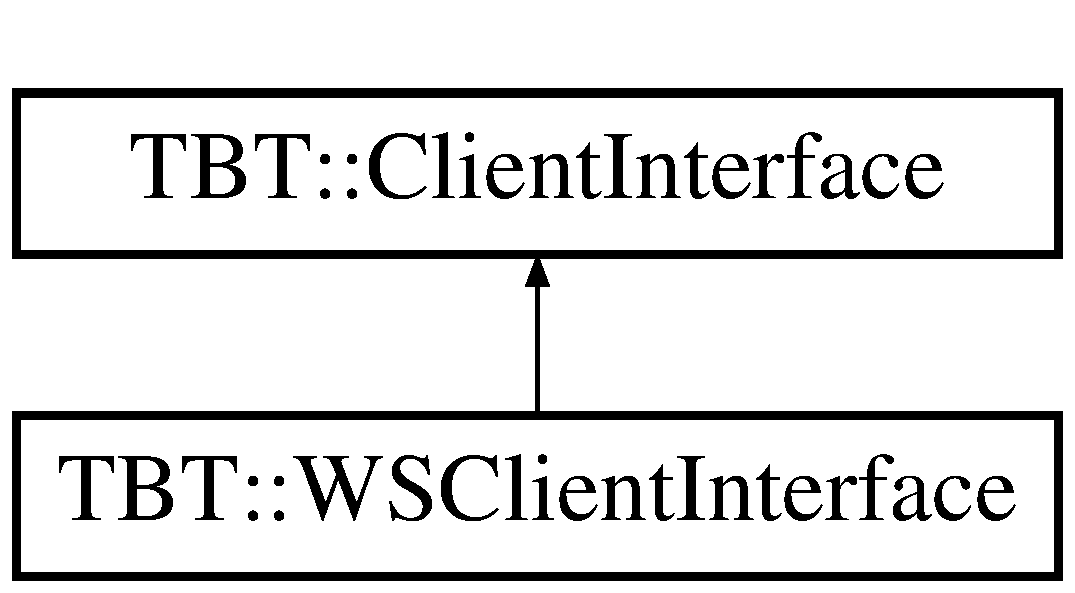
\includegraphics[height=2.000000cm]{classTBT_1_1WSClientInterface}
\end{center}
\end{figure}
\subsection*{Public Member Functions}
\begin{DoxyCompactItemize}
\item 
\mbox{\Hypertarget{classTBT_1_1WSClientInterface_addd44890c3c54a9700a2385a63105e38}\label{classTBT_1_1WSClientInterface_addd44890c3c54a9700a2385a63105e38}} 
{\bfseries W\+S\+Client\+Interface} (\hyperlink{classTBT_1_1Manager}{Manager} $\ast$p\+Manager, const char $\ast$port=W\+S\+\_\+\+P\+O\+RT)
\item 
\mbox{\Hypertarget{classTBT_1_1WSClientInterface_ad5ff4048859e3bf2fe8c62b9b2c59080}\label{classTBT_1_1WSClientInterface_ad5ff4048859e3bf2fe8c62b9b2c59080}} 
virtual void {\bfseries broadcast\+Power\+State\+Change} (Power\+State new\+State)
\item 
\mbox{\Hypertarget{classTBT_1_1WSClientInterface_a39806206461815c06c517b66d122b4db}\label{classTBT_1_1WSClientInterface_a39806206461815c06c517b66d122b4db}} 
virtual void {\bfseries broadcast\+Loc\+Info\+Change} (\hyperlink{classTBT_1_1LocDecoder}{Loc\+Decoder} $\ast$p\+Loc)
\item 
\mbox{\Hypertarget{classTBT_1_1WSClientInterface_a328ee22796e058e0da825e5f13349e1f}\label{classTBT_1_1WSClientInterface_a328ee22796e058e0da825e5f13349e1f}} 
virtual void {\bfseries broadcast\+Emergency\+Stop} (bool stop)
\end{DoxyCompactItemize}
\subsection*{Protected Attributes}
\begin{DoxyCompactItemize}
\item 
\mbox{\Hypertarget{classTBT_1_1WSClientInterface_a5a2b51f344e17b5f3e9b1f3e861b6efe}\label{classTBT_1_1WSClientInterface_a5a2b51f344e17b5f3e9b1f3e861b6efe}} 
char $\ast$ {\bfseries m\+\_\+port}
\item 
\mbox{\Hypertarget{classTBT_1_1WSClientInterface_a888e4be88a311199a3fa890d3abc6a10}\label{classTBT_1_1WSClientInterface_a888e4be88a311199a3fa890d3abc6a10}} 
volatile bool {\bfseries m\+\_\+b\+Continue}
\item 
\mbox{\Hypertarget{classTBT_1_1WSClientInterface_af8db3d6b3e3923b0b61f43cbc2021a92}\label{classTBT_1_1WSClientInterface_af8db3d6b3e3923b0b61f43cbc2021a92}} 
thread {\bfseries m\+\_\+thread}
\item 
\mbox{\Hypertarget{classTBT_1_1WSClientInterface_aba2e99d7dcc90848ce6348ee687affbb}\label{classTBT_1_1WSClientInterface_aba2e99d7dcc90848ce6348ee687affbb}} 
\hyperlink{structmg__mgr}{mg\+\_\+mgr} {\bfseries m\+\_\+mgr}
\item 
\mbox{\Hypertarget{classTBT_1_1WSClientInterface_ae866ad6fbf964a4b6ad1e19895bb24be}\label{classTBT_1_1WSClientInterface_ae866ad6fbf964a4b6ad1e19895bb24be}} 
\hyperlink{structmg__connection}{mg\+\_\+connection} $\ast$ {\bfseries m\+\_\+conn}
\end{DoxyCompactItemize}


The documentation for this class was generated from the following files\+:\begin{DoxyCompactItemize}
\item 
W\+S\+Client\+Interface.\+h\item 
W\+S\+Client\+Interface.\+cpp\end{DoxyCompactItemize}

\hypertarget{classTBT_1_1XpressNetClient}{}\section{T\+BT\+:\+:Xpress\+Net\+Client Class Reference}
\label{classTBT_1_1XpressNetClient}\index{T\+B\+T\+::\+Xpress\+Net\+Client@{T\+B\+T\+::\+Xpress\+Net\+Client}}


{\ttfamily \#include $<$Xpress\+Net\+Client.\+h$>$}

Inheritance diagram for T\+BT\+:\+:Xpress\+Net\+Client\+:\begin{figure}[H]
\begin{center}
\leavevmode
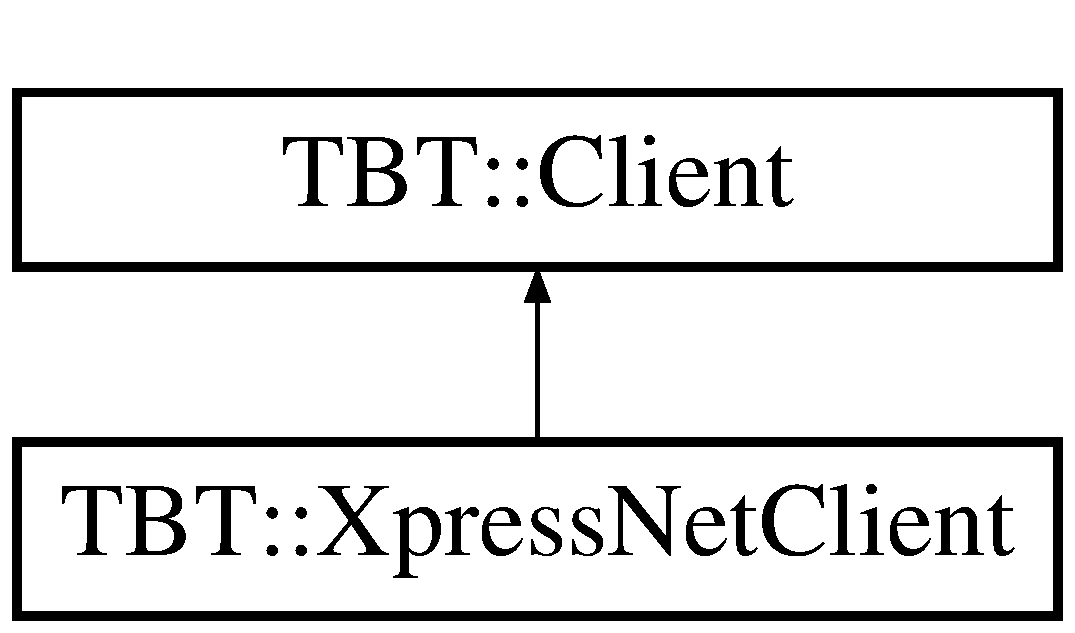
\includegraphics[height=2.000000cm]{classTBT_1_1XpressNetClient}
\end{center}
\end{figure}
\subsection*{Public Member Functions}
\begin{DoxyCompactItemize}
\item 
\hyperlink{classTBT_1_1XpressNetClient_a7647a4b5b68c29a2ed7d8832b6d1b692_a7647a4b5b68c29a2ed7d8832b6d1b692}{Xpress\+Net\+Client} (\hyperlink{classTBT_1_1ClientInterface}{Client\+Interface} $\ast$p\+Interface, uint8\+\_\+t Xpress\+Net\+Address)
\item 
virtual \hyperlink{classTBT_1_1XpressNetClient_a6c8fe1f6815ddbf26141d3ed7cdb072c_a6c8fe1f6815ddbf26141d3ed7cdb072c}{$\sim$\+Xpress\+Net\+Client} ()
\item 
const uint8\+\_\+t \& \hyperlink{classTBT_1_1XpressNetClient_aae838c0fdb74c9c7220056e3fa011390_aae838c0fdb74c9c7220056e3fa011390}{get\+Address} (void)
\item 
virtual void \hyperlink{classTBT_1_1XpressNetClient_a6f104050aad16ef336a6b83d2c60550a_a6f104050aad16ef336a6b83d2c60550a}{broadcast\+Power\+State\+Change} (bool new\+State)
\item 
virtual void \hyperlink{classTBT_1_1XpressNetClient_a0ef986da287d7fbfea163ae6016a7154_a0ef986da287d7fbfea163ae6016a7154}{broadcast\+Loc\+Info\+Changed} (\hyperlink{classTBT_1_1LocDecoder}{Loc\+Decoder} $\ast$p\+Loc)
\item 
virtual void \hyperlink{classTBT_1_1XpressNetClient_a5909e439836c772127bc24918aa0a291_a5909e439836c772127bc24918aa0a291}{broadcast\+Emergency\+Stop} (void)
\end{DoxyCompactItemize}
\subsection*{Protected Attributes}
\begin{DoxyCompactItemize}
\item 
uint8\+\_\+t \hyperlink{classTBT_1_1XpressNetClient_a9af9cd4bed2191d7504b8ae480182643_a9af9cd4bed2191d7504b8ae480182643}{m\+\_\+\+Xpress\+Net\+Address}
\end{DoxyCompactItemize}


\subsection{Constructor \& Destructor Documentation}
\mbox{\Hypertarget{classTBT_1_1XpressNetClient_a7647a4b5b68c29a2ed7d8832b6d1b692_a7647a4b5b68c29a2ed7d8832b6d1b692}\label{classTBT_1_1XpressNetClient_a7647a4b5b68c29a2ed7d8832b6d1b692_a7647a4b5b68c29a2ed7d8832b6d1b692}} 
\index{T\+B\+T\+::\+Xpress\+Net\+Client@{T\+B\+T\+::\+Xpress\+Net\+Client}!Xpress\+Net\+Client@{Xpress\+Net\+Client}}
\index{Xpress\+Net\+Client@{Xpress\+Net\+Client}!T\+B\+T\+::\+Xpress\+Net\+Client@{T\+B\+T\+::\+Xpress\+Net\+Client}}
\subsubsection{\texorpdfstring{Xpress\+Net\+Client()}{XpressNetClient()}}
{\footnotesize\ttfamily T\+B\+T\+::\+Xpress\+Net\+Client\+::\+Xpress\+Net\+Client (\begin{DoxyParamCaption}\item[{\hyperlink{classTBT_1_1ClientInterface}{Client\+Interface} $\ast$}]{p\+Interface,  }\item[{uint8\+\_\+t}]{Xpress\+Net\+Address }\end{DoxyParamCaption})}

\mbox{\Hypertarget{classTBT_1_1XpressNetClient_a6c8fe1f6815ddbf26141d3ed7cdb072c_a6c8fe1f6815ddbf26141d3ed7cdb072c}\label{classTBT_1_1XpressNetClient_a6c8fe1f6815ddbf26141d3ed7cdb072c_a6c8fe1f6815ddbf26141d3ed7cdb072c}} 
\index{T\+B\+T\+::\+Xpress\+Net\+Client@{T\+B\+T\+::\+Xpress\+Net\+Client}!````~Xpress\+Net\+Client@{$\sim$\+Xpress\+Net\+Client}}
\index{````~Xpress\+Net\+Client@{$\sim$\+Xpress\+Net\+Client}!T\+B\+T\+::\+Xpress\+Net\+Client@{T\+B\+T\+::\+Xpress\+Net\+Client}}
\subsubsection{\texorpdfstring{$\sim$\+Xpress\+Net\+Client()}{~XpressNetClient()}}
{\footnotesize\ttfamily T\+B\+T\+::\+Xpress\+Net\+Client\+::$\sim$\+Xpress\+Net\+Client (\begin{DoxyParamCaption}{ }\end{DoxyParamCaption})\hspace{0.3cm}{\ttfamily [virtual]}}



\subsection{Member Function Documentation}
\mbox{\Hypertarget{classTBT_1_1XpressNetClient_a5909e439836c772127bc24918aa0a291_a5909e439836c772127bc24918aa0a291}\label{classTBT_1_1XpressNetClient_a5909e439836c772127bc24918aa0a291_a5909e439836c772127bc24918aa0a291}} 
\index{T\+B\+T\+::\+Xpress\+Net\+Client@{T\+B\+T\+::\+Xpress\+Net\+Client}!broadcast\+Emergency\+Stop@{broadcast\+Emergency\+Stop}}
\index{broadcast\+Emergency\+Stop@{broadcast\+Emergency\+Stop}!T\+B\+T\+::\+Xpress\+Net\+Client@{T\+B\+T\+::\+Xpress\+Net\+Client}}
\subsubsection{\texorpdfstring{broadcast\+Emergency\+Stop()}{broadcastEmergencyStop()}}
{\footnotesize\ttfamily virtual void T\+B\+T\+::\+Xpress\+Net\+Client\+::broadcast\+Emergency\+Stop (\begin{DoxyParamCaption}\item[{void}]{ }\end{DoxyParamCaption})\hspace{0.3cm}{\ttfamily [inline]}, {\ttfamily [virtual]}}



Implements \hyperlink{classTBT_1_1Client_a59459df809a663bcbbb6d31fbfa09402_a59459df809a663bcbbb6d31fbfa09402}{T\+B\+T\+::\+Client}.

\mbox{\Hypertarget{classTBT_1_1XpressNetClient_a0ef986da287d7fbfea163ae6016a7154_a0ef986da287d7fbfea163ae6016a7154}\label{classTBT_1_1XpressNetClient_a0ef986da287d7fbfea163ae6016a7154_a0ef986da287d7fbfea163ae6016a7154}} 
\index{T\+B\+T\+::\+Xpress\+Net\+Client@{T\+B\+T\+::\+Xpress\+Net\+Client}!broadcast\+Loc\+Info\+Changed@{broadcast\+Loc\+Info\+Changed}}
\index{broadcast\+Loc\+Info\+Changed@{broadcast\+Loc\+Info\+Changed}!T\+B\+T\+::\+Xpress\+Net\+Client@{T\+B\+T\+::\+Xpress\+Net\+Client}}
\subsubsection{\texorpdfstring{broadcast\+Loc\+Info\+Changed()}{broadcastLocInfoChanged()}}
{\footnotesize\ttfamily void T\+B\+T\+::\+Xpress\+Net\+Client\+::broadcast\+Loc\+Info\+Changed (\begin{DoxyParamCaption}\item[{\hyperlink{classTBT_1_1LocDecoder}{Loc\+Decoder} $\ast$}]{p\+Loc }\end{DoxyParamCaption})\hspace{0.3cm}{\ttfamily [virtual]}}



Implements \hyperlink{classTBT_1_1Client_aeb3b63a37edc6b95872df54a57c27a71_aeb3b63a37edc6b95872df54a57c27a71}{T\+B\+T\+::\+Client}.



Referenced by get\+Address().

\mbox{\Hypertarget{classTBT_1_1XpressNetClient_a6f104050aad16ef336a6b83d2c60550a_a6f104050aad16ef336a6b83d2c60550a}\label{classTBT_1_1XpressNetClient_a6f104050aad16ef336a6b83d2c60550a_a6f104050aad16ef336a6b83d2c60550a}} 
\index{T\+B\+T\+::\+Xpress\+Net\+Client@{T\+B\+T\+::\+Xpress\+Net\+Client}!broadcast\+Power\+State\+Change@{broadcast\+Power\+State\+Change}}
\index{broadcast\+Power\+State\+Change@{broadcast\+Power\+State\+Change}!T\+B\+T\+::\+Xpress\+Net\+Client@{T\+B\+T\+::\+Xpress\+Net\+Client}}
\subsubsection{\texorpdfstring{broadcast\+Power\+State\+Change()}{broadcastPowerStateChange()}}
{\footnotesize\ttfamily void T\+B\+T\+::\+Xpress\+Net\+Client\+::broadcast\+Power\+State\+Change (\begin{DoxyParamCaption}\item[{bool}]{new\+State }\end{DoxyParamCaption})\hspace{0.3cm}{\ttfamily [virtual]}}



Implements \hyperlink{classTBT_1_1Client_ad64588b494ec98154ea261ed4f3b3643_ad64588b494ec98154ea261ed4f3b3643}{T\+B\+T\+::\+Client}.



Referenced by get\+Address().

\mbox{\Hypertarget{classTBT_1_1XpressNetClient_aae838c0fdb74c9c7220056e3fa011390_aae838c0fdb74c9c7220056e3fa011390}\label{classTBT_1_1XpressNetClient_aae838c0fdb74c9c7220056e3fa011390_aae838c0fdb74c9c7220056e3fa011390}} 
\index{T\+B\+T\+::\+Xpress\+Net\+Client@{T\+B\+T\+::\+Xpress\+Net\+Client}!get\+Address@{get\+Address}}
\index{get\+Address@{get\+Address}!T\+B\+T\+::\+Xpress\+Net\+Client@{T\+B\+T\+::\+Xpress\+Net\+Client}}
\subsubsection{\texorpdfstring{get\+Address()}{getAddress()}}
{\footnotesize\ttfamily const uint8\+\_\+t\& T\+B\+T\+::\+Xpress\+Net\+Client\+::get\+Address (\begin{DoxyParamCaption}\item[{void}]{ }\end{DoxyParamCaption})\hspace{0.3cm}{\ttfamily [inline]}}



References broadcast\+Loc\+Info\+Changed(), broadcast\+Power\+State\+Change(), and m\+\_\+\+Xpress\+Net\+Address.



\subsection{Member Data Documentation}
\mbox{\Hypertarget{classTBT_1_1XpressNetClient_a9af9cd4bed2191d7504b8ae480182643_a9af9cd4bed2191d7504b8ae480182643}\label{classTBT_1_1XpressNetClient_a9af9cd4bed2191d7504b8ae480182643_a9af9cd4bed2191d7504b8ae480182643}} 
\index{T\+B\+T\+::\+Xpress\+Net\+Client@{T\+B\+T\+::\+Xpress\+Net\+Client}!m\+\_\+\+Xpress\+Net\+Address@{m\+\_\+\+Xpress\+Net\+Address}}
\index{m\+\_\+\+Xpress\+Net\+Address@{m\+\_\+\+Xpress\+Net\+Address}!T\+B\+T\+::\+Xpress\+Net\+Client@{T\+B\+T\+::\+Xpress\+Net\+Client}}
\subsubsection{\texorpdfstring{m\+\_\+\+Xpress\+Net\+Address}{m\_XpressNetAddress}}
{\footnotesize\ttfamily uint8\+\_\+t T\+B\+T\+::\+Xpress\+Net\+Client\+::m\+\_\+\+Xpress\+Net\+Address\hspace{0.3cm}{\ttfamily [protected]}}



Referenced by get\+Address().



The documentation for this class was generated from the following files\+:\begin{DoxyCompactItemize}
\item 
\hyperlink{XpressNetClient_8h}{Xpress\+Net\+Client.\+h}\item 
\hyperlink{XpressNetClient_8cpp}{Xpress\+Net\+Client.\+cpp}\end{DoxyCompactItemize}

\hypertarget{classTBT_1_1XpressNetClientInterface}{}\section{T\+BT\+:\+:Xpress\+Net\+Client\+Interface Class Reference}
\label{classTBT_1_1XpressNetClientInterface}\index{T\+B\+T\+::\+Xpress\+Net\+Client\+Interface@{T\+B\+T\+::\+Xpress\+Net\+Client\+Interface}}


{\ttfamily \#include $<$Xpress\+Net\+Client\+Interface.\+h$>$}

Inheritance diagram for T\+BT\+:\+:Xpress\+Net\+Client\+Interface\+:\begin{figure}[H]
\begin{center}
\leavevmode
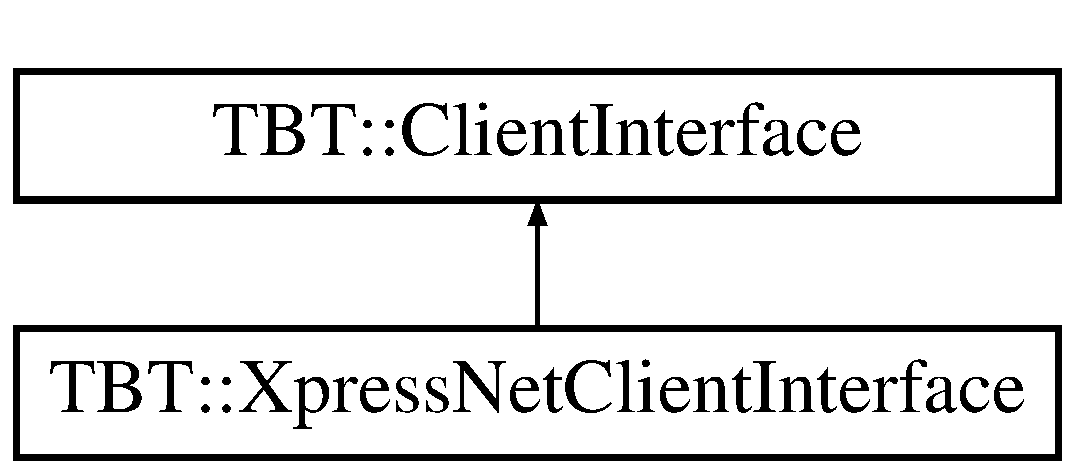
\includegraphics[height=2.000000cm]{classTBT_1_1XpressNetClientInterface}
\end{center}
\end{figure}
\subsection*{Public Member Functions}
\begin{DoxyCompactItemize}
\item 
\hyperlink{classTBT_1_1XpressNetClientInterface_afc3950ffc2b045e653c539a57967aa57_afc3950ffc2b045e653c539a57967aa57}{Xpress\+Net\+Client\+Interface} (\hyperlink{classTBT_1_1Manager}{Manager} $\ast$p\+Manager, const char $\ast$tty\+Path=\char`\"{}/dev/tty\+O1\char`\"{})
\item 
virtual \hyperlink{classTBT_1_1XpressNetClientInterface_a83f7c569ae4f17e8d9c06671166e635f_a83f7c569ae4f17e8d9c06671166e635f}{$\sim$\+Xpress\+Net\+Client\+Interface} ()
\item 
virtual void \hyperlink{classTBT_1_1XpressNetClientInterface_a338da1925ec68f197e87625c7497f472_a338da1925ec68f197e87625c7497f472}{broadcast\+Power\+State\+Change} (bool new\+State)
\item 
virtual void \hyperlink{classTBT_1_1XpressNetClientInterface_a8e64404cb84913c2d9290d2afb882b39_a8e64404cb84913c2d9290d2afb882b39}{broadcast\+Loc\+Info\+Change} (\hyperlink{classTBT_1_1LocDecoder}{Loc\+Decoder} $\ast$p\+Loc)
\item 
virtual void \hyperlink{classTBT_1_1XpressNetClientInterface_a143641241f4830f22ec5beb78036ce4c_a143641241f4830f22ec5beb78036ce4c}{broadcast\+Emergency\+Stop} (void)
\end{DoxyCompactItemize}
\subsection*{Protected Member Functions}
\begin{DoxyCompactItemize}
\item 
\hyperlink{classTBT_1_1XpressNetClient}{Xpress\+Net\+Client} $\ast$ \hyperlink{classTBT_1_1XpressNetClientInterface_ac7c05010e7a1cb8fe251c0154ca421d3_ac7c05010e7a1cb8fe251c0154ca421d3}{find\+Client} (const uint8\+\_\+t \&address)
\end{DoxyCompactItemize}
\subsection*{Private Member Functions}
\begin{DoxyCompactItemize}
\item 
void \hyperlink{classTBT_1_1XpressNetClientInterface_a8b49b38dfe0d208f643f7c65d380f31b_a8b49b38dfe0d208f643f7c65d380f31b}{thread\+Func} (void)
\end{DoxyCompactItemize}
\subsection*{Private Attributes}
\begin{DoxyCompactItemize}
\item 
char $\ast$ \hyperlink{classTBT_1_1XpressNetClientInterface_afce6612b04b468e20f8196a73bd16c7b_afce6612b04b468e20f8196a73bd16c7b}{m\+\_\+p\+Tty\+Path}
\item 
int \hyperlink{classTBT_1_1XpressNetClientInterface_a860a0570de71822774ab9d1ff14d459a_a860a0570de71822774ab9d1ff14d459a}{m\+\_\+fd\+Serial}
\item 
int \hyperlink{classTBT_1_1XpressNetClientInterface_a2a7be080da9167700fdaadbba29f1f8e_a2a7be080da9167700fdaadbba29f1f8e}{m\+\_\+fd\+Stop}
\item 
thread \hyperlink{classTBT_1_1XpressNetClientInterface_a7ed370b795990420b49cb201f3cb5c60_a7ed370b795990420b49cb201f3cb5c60}{m\+\_\+thread}
\item 
map$<$ uint8\+\_\+t, \hyperlink{classTBT_1_1XpressNetClient}{Xpress\+Net\+Client} $\ast$ $>$ \hyperlink{classTBT_1_1XpressNetClientInterface_ac064949432059e1c5210c56b43bb1168_ac064949432059e1c5210c56b43bb1168}{m\+\_\+\+Clients}
\item 
recursive\+\_\+mutex \hyperlink{classTBT_1_1XpressNetClientInterface_a22f7ef7cb7428cf26544df1bc336d517_a22f7ef7cb7428cf26544df1bc336d517}{m\+\_\+\+M\+Clients}
\end{DoxyCompactItemize}
\subsection*{Additional Inherited Members}


\subsection{Constructor \& Destructor Documentation}
\mbox{\Hypertarget{classTBT_1_1XpressNetClientInterface_afc3950ffc2b045e653c539a57967aa57_afc3950ffc2b045e653c539a57967aa57}\label{classTBT_1_1XpressNetClientInterface_afc3950ffc2b045e653c539a57967aa57_afc3950ffc2b045e653c539a57967aa57}} 
\index{T\+B\+T\+::\+Xpress\+Net\+Client\+Interface@{T\+B\+T\+::\+Xpress\+Net\+Client\+Interface}!Xpress\+Net\+Client\+Interface@{Xpress\+Net\+Client\+Interface}}
\index{Xpress\+Net\+Client\+Interface@{Xpress\+Net\+Client\+Interface}!T\+B\+T\+::\+Xpress\+Net\+Client\+Interface@{T\+B\+T\+::\+Xpress\+Net\+Client\+Interface}}
\subsubsection{\texorpdfstring{Xpress\+Net\+Client\+Interface()}{XpressNetClientInterface()}}
{\footnotesize\ttfamily T\+B\+T\+::\+Xpress\+Net\+Client\+Interface\+::\+Xpress\+Net\+Client\+Interface (\begin{DoxyParamCaption}\item[{\hyperlink{classTBT_1_1Manager}{Manager} $\ast$}]{p\+Manager,  }\item[{const char $\ast$}]{tty\+Path = {\ttfamily \char`\"{}/dev/ttyO1\char`\"{}} }\end{DoxyParamCaption})}



References m\+\_\+fd\+Serial, m\+\_\+fd\+Stop, m\+\_\+p\+Tty\+Path, m\+\_\+thread, and thread\+Func().

\mbox{\Hypertarget{classTBT_1_1XpressNetClientInterface_a83f7c569ae4f17e8d9c06671166e635f_a83f7c569ae4f17e8d9c06671166e635f}\label{classTBT_1_1XpressNetClientInterface_a83f7c569ae4f17e8d9c06671166e635f_a83f7c569ae4f17e8d9c06671166e635f}} 
\index{T\+B\+T\+::\+Xpress\+Net\+Client\+Interface@{T\+B\+T\+::\+Xpress\+Net\+Client\+Interface}!````~Xpress\+Net\+Client\+Interface@{$\sim$\+Xpress\+Net\+Client\+Interface}}
\index{````~Xpress\+Net\+Client\+Interface@{$\sim$\+Xpress\+Net\+Client\+Interface}!T\+B\+T\+::\+Xpress\+Net\+Client\+Interface@{T\+B\+T\+::\+Xpress\+Net\+Client\+Interface}}
\subsubsection{\texorpdfstring{$\sim$\+Xpress\+Net\+Client\+Interface()}{~XpressNetClientInterface()}}
{\footnotesize\ttfamily T\+B\+T\+::\+Xpress\+Net\+Client\+Interface\+::$\sim$\+Xpress\+Net\+Client\+Interface (\begin{DoxyParamCaption}{ }\end{DoxyParamCaption})\hspace{0.3cm}{\ttfamily [virtual]}}



References m\+\_\+fd\+Serial, m\+\_\+fd\+Stop, m\+\_\+p\+Tty\+Path, and m\+\_\+thread.



\subsection{Member Function Documentation}
\mbox{\Hypertarget{classTBT_1_1XpressNetClientInterface_a143641241f4830f22ec5beb78036ce4c_a143641241f4830f22ec5beb78036ce4c}\label{classTBT_1_1XpressNetClientInterface_a143641241f4830f22ec5beb78036ce4c_a143641241f4830f22ec5beb78036ce4c}} 
\index{T\+B\+T\+::\+Xpress\+Net\+Client\+Interface@{T\+B\+T\+::\+Xpress\+Net\+Client\+Interface}!broadcast\+Emergency\+Stop@{broadcast\+Emergency\+Stop}}
\index{broadcast\+Emergency\+Stop@{broadcast\+Emergency\+Stop}!T\+B\+T\+::\+Xpress\+Net\+Client\+Interface@{T\+B\+T\+::\+Xpress\+Net\+Client\+Interface}}
\subsubsection{\texorpdfstring{broadcast\+Emergency\+Stop()}{broadcastEmergencyStop()}}
{\footnotesize\ttfamily void T\+B\+T\+::\+Xpress\+Net\+Client\+Interface\+::broadcast\+Emergency\+Stop (\begin{DoxyParamCaption}\item[{void}]{ }\end{DoxyParamCaption})\hspace{0.3cm}{\ttfamily [virtual]}}



Implements \hyperlink{classTBT_1_1ClientInterface_a8d19220baccb47a7c9f45d0288bebcb8_a8d19220baccb47a7c9f45d0288bebcb8}{T\+B\+T\+::\+Client\+Interface}.



References m\+\_\+fd\+Serial.

\mbox{\Hypertarget{classTBT_1_1XpressNetClientInterface_a8e64404cb84913c2d9290d2afb882b39_a8e64404cb84913c2d9290d2afb882b39}\label{classTBT_1_1XpressNetClientInterface_a8e64404cb84913c2d9290d2afb882b39_a8e64404cb84913c2d9290d2afb882b39}} 
\index{T\+B\+T\+::\+Xpress\+Net\+Client\+Interface@{T\+B\+T\+::\+Xpress\+Net\+Client\+Interface}!broadcast\+Loc\+Info\+Change@{broadcast\+Loc\+Info\+Change}}
\index{broadcast\+Loc\+Info\+Change@{broadcast\+Loc\+Info\+Change}!T\+B\+T\+::\+Xpress\+Net\+Client\+Interface@{T\+B\+T\+::\+Xpress\+Net\+Client\+Interface}}
\subsubsection{\texorpdfstring{broadcast\+Loc\+Info\+Change()}{broadcastLocInfoChange()}}
{\footnotesize\ttfamily void T\+B\+T\+::\+Xpress\+Net\+Client\+Interface\+::broadcast\+Loc\+Info\+Change (\begin{DoxyParamCaption}\item[{\hyperlink{classTBT_1_1LocDecoder}{Loc\+Decoder} $\ast$}]{p\+Loc }\end{DoxyParamCaption})\hspace{0.3cm}{\ttfamily [virtual]}}



Implements \hyperlink{classTBT_1_1ClientInterface_aaede3709fa0dcb23743f43d9c1a5ab04_aaede3709fa0dcb23743f43d9c1a5ab04}{T\+B\+T\+::\+Client\+Interface}.

\mbox{\Hypertarget{classTBT_1_1XpressNetClientInterface_a338da1925ec68f197e87625c7497f472_a338da1925ec68f197e87625c7497f472}\label{classTBT_1_1XpressNetClientInterface_a338da1925ec68f197e87625c7497f472_a338da1925ec68f197e87625c7497f472}} 
\index{T\+B\+T\+::\+Xpress\+Net\+Client\+Interface@{T\+B\+T\+::\+Xpress\+Net\+Client\+Interface}!broadcast\+Power\+State\+Change@{broadcast\+Power\+State\+Change}}
\index{broadcast\+Power\+State\+Change@{broadcast\+Power\+State\+Change}!T\+B\+T\+::\+Xpress\+Net\+Client\+Interface@{T\+B\+T\+::\+Xpress\+Net\+Client\+Interface}}
\subsubsection{\texorpdfstring{broadcast\+Power\+State\+Change()}{broadcastPowerStateChange()}}
{\footnotesize\ttfamily void T\+B\+T\+::\+Xpress\+Net\+Client\+Interface\+::broadcast\+Power\+State\+Change (\begin{DoxyParamCaption}\item[{bool}]{new\+State }\end{DoxyParamCaption})\hspace{0.3cm}{\ttfamily [virtual]}}



Implements \hyperlink{classTBT_1_1ClientInterface_a7888a3446fb416fad75e5e008a85ca0c_a7888a3446fb416fad75e5e008a85ca0c}{T\+B\+T\+::\+Client\+Interface}.



References m\+\_\+fd\+Serial.

\mbox{\Hypertarget{classTBT_1_1XpressNetClientInterface_ac7c05010e7a1cb8fe251c0154ca421d3_ac7c05010e7a1cb8fe251c0154ca421d3}\label{classTBT_1_1XpressNetClientInterface_ac7c05010e7a1cb8fe251c0154ca421d3_ac7c05010e7a1cb8fe251c0154ca421d3}} 
\index{T\+B\+T\+::\+Xpress\+Net\+Client\+Interface@{T\+B\+T\+::\+Xpress\+Net\+Client\+Interface}!find\+Client@{find\+Client}}
\index{find\+Client@{find\+Client}!T\+B\+T\+::\+Xpress\+Net\+Client\+Interface@{T\+B\+T\+::\+Xpress\+Net\+Client\+Interface}}
\subsubsection{\texorpdfstring{find\+Client()}{findClient()}}
{\footnotesize\ttfamily \hyperlink{classTBT_1_1XpressNetClient}{Xpress\+Net\+Client} $\ast$ T\+B\+T\+::\+Xpress\+Net\+Client\+Interface\+::find\+Client (\begin{DoxyParamCaption}\item[{const uint8\+\_\+t \&}]{address }\end{DoxyParamCaption})\hspace{0.3cm}{\ttfamily [protected]}}



References m\+\_\+\+Clients, and m\+\_\+\+M\+Clients.



Referenced by thread\+Func().

\mbox{\Hypertarget{classTBT_1_1XpressNetClientInterface_a8b49b38dfe0d208f643f7c65d380f31b_a8b49b38dfe0d208f643f7c65d380f31b}\label{classTBT_1_1XpressNetClientInterface_a8b49b38dfe0d208f643f7c65d380f31b_a8b49b38dfe0d208f643f7c65d380f31b}} 
\index{T\+B\+T\+::\+Xpress\+Net\+Client\+Interface@{T\+B\+T\+::\+Xpress\+Net\+Client\+Interface}!thread\+Func@{thread\+Func}}
\index{thread\+Func@{thread\+Func}!T\+B\+T\+::\+Xpress\+Net\+Client\+Interface@{T\+B\+T\+::\+Xpress\+Net\+Client\+Interface}}
\subsubsection{\texorpdfstring{thread\+Func()}{threadFunc()}}
{\footnotesize\ttfamily void T\+B\+T\+::\+Xpress\+Net\+Client\+Interface\+::thread\+Func (\begin{DoxyParamCaption}\item[{void}]{ }\end{DoxyParamCaption})\hspace{0.3cm}{\ttfamily [private]}}



References find\+Client(), T\+B\+T\+::\+Manager\+::find\+Decoder(), T\+B\+T\+::\+Manager\+::get\+Central\+State(), T\+B\+T\+::\+Client\+::get\+Interface(), T\+B\+T\+::\+Client\+Interface\+::get\+Manager(), T\+B\+T\+::\+Loc\+Decoder\+::get\+Speedsteps(), m\+\_\+fd\+Serial, m\+\_\+fd\+Stop, N\+B\+R\+X\+P\+R\+E\+S\+S\+N\+E\+T\+P\+O\+L\+L\+E\+V\+E\+N\+TS, T\+B\+T\+::\+Power\+Off, T\+B\+T\+::\+Power\+On, T\+B\+T\+::\+Manager\+::set\+Emergency\+Stop(), T\+B\+T\+::\+Loc\+Decoder\+::set\+Function\+Group1(), T\+B\+T\+::\+Loc\+Decoder\+::set\+Function\+Group2(), T\+B\+T\+::\+Loc\+Decoder\+::set\+Function\+Group3(), T\+B\+T\+::\+Loc\+Decoder\+::set\+Function\+Group4(), T\+B\+T\+::\+Loc\+Decoder\+::set\+Function\+Group5(), T\+B\+T\+::\+Loc\+Decoder\+::set\+Loco\+Drive128(), T\+B\+T\+::\+Loc\+Decoder\+::set\+Loco\+Drive14(), T\+B\+T\+::\+Loc\+Decoder\+::set\+Loco\+Drive27(), T\+B\+T\+::\+Loc\+Decoder\+::set\+Loco\+Drive28(), and T\+B\+T\+::\+Manager\+::set\+Power\+State().



Referenced by Xpress\+Net\+Client\+Interface().



\subsection{Member Data Documentation}
\mbox{\Hypertarget{classTBT_1_1XpressNetClientInterface_ac064949432059e1c5210c56b43bb1168_ac064949432059e1c5210c56b43bb1168}\label{classTBT_1_1XpressNetClientInterface_ac064949432059e1c5210c56b43bb1168_ac064949432059e1c5210c56b43bb1168}} 
\index{T\+B\+T\+::\+Xpress\+Net\+Client\+Interface@{T\+B\+T\+::\+Xpress\+Net\+Client\+Interface}!m\+\_\+\+Clients@{m\+\_\+\+Clients}}
\index{m\+\_\+\+Clients@{m\+\_\+\+Clients}!T\+B\+T\+::\+Xpress\+Net\+Client\+Interface@{T\+B\+T\+::\+Xpress\+Net\+Client\+Interface}}
\subsubsection{\texorpdfstring{m\+\_\+\+Clients}{m\_Clients}}
{\footnotesize\ttfamily map$<$uint8\+\_\+t, \hyperlink{classTBT_1_1XpressNetClient}{Xpress\+Net\+Client}$\ast$$>$ T\+B\+T\+::\+Xpress\+Net\+Client\+Interface\+::m\+\_\+\+Clients\hspace{0.3cm}{\ttfamily [private]}}



Referenced by find\+Client().

\mbox{\Hypertarget{classTBT_1_1XpressNetClientInterface_a860a0570de71822774ab9d1ff14d459a_a860a0570de71822774ab9d1ff14d459a}\label{classTBT_1_1XpressNetClientInterface_a860a0570de71822774ab9d1ff14d459a_a860a0570de71822774ab9d1ff14d459a}} 
\index{T\+B\+T\+::\+Xpress\+Net\+Client\+Interface@{T\+B\+T\+::\+Xpress\+Net\+Client\+Interface}!m\+\_\+fd\+Serial@{m\+\_\+fd\+Serial}}
\index{m\+\_\+fd\+Serial@{m\+\_\+fd\+Serial}!T\+B\+T\+::\+Xpress\+Net\+Client\+Interface@{T\+B\+T\+::\+Xpress\+Net\+Client\+Interface}}
\subsubsection{\texorpdfstring{m\+\_\+fd\+Serial}{m\_fdSerial}}
{\footnotesize\ttfamily int T\+B\+T\+::\+Xpress\+Net\+Client\+Interface\+::m\+\_\+fd\+Serial\hspace{0.3cm}{\ttfamily [private]}}



Referenced by broadcast\+Emergency\+Stop(), broadcast\+Power\+State\+Change(), thread\+Func(), Xpress\+Net\+Client\+Interface(), and $\sim$\+Xpress\+Net\+Client\+Interface().

\mbox{\Hypertarget{classTBT_1_1XpressNetClientInterface_a2a7be080da9167700fdaadbba29f1f8e_a2a7be080da9167700fdaadbba29f1f8e}\label{classTBT_1_1XpressNetClientInterface_a2a7be080da9167700fdaadbba29f1f8e_a2a7be080da9167700fdaadbba29f1f8e}} 
\index{T\+B\+T\+::\+Xpress\+Net\+Client\+Interface@{T\+B\+T\+::\+Xpress\+Net\+Client\+Interface}!m\+\_\+fd\+Stop@{m\+\_\+fd\+Stop}}
\index{m\+\_\+fd\+Stop@{m\+\_\+fd\+Stop}!T\+B\+T\+::\+Xpress\+Net\+Client\+Interface@{T\+B\+T\+::\+Xpress\+Net\+Client\+Interface}}
\subsubsection{\texorpdfstring{m\+\_\+fd\+Stop}{m\_fdStop}}
{\footnotesize\ttfamily int T\+B\+T\+::\+Xpress\+Net\+Client\+Interface\+::m\+\_\+fd\+Stop\hspace{0.3cm}{\ttfamily [private]}}



Referenced by thread\+Func(), Xpress\+Net\+Client\+Interface(), and $\sim$\+Xpress\+Net\+Client\+Interface().

\mbox{\Hypertarget{classTBT_1_1XpressNetClientInterface_a22f7ef7cb7428cf26544df1bc336d517_a22f7ef7cb7428cf26544df1bc336d517}\label{classTBT_1_1XpressNetClientInterface_a22f7ef7cb7428cf26544df1bc336d517_a22f7ef7cb7428cf26544df1bc336d517}} 
\index{T\+B\+T\+::\+Xpress\+Net\+Client\+Interface@{T\+B\+T\+::\+Xpress\+Net\+Client\+Interface}!m\+\_\+\+M\+Clients@{m\+\_\+\+M\+Clients}}
\index{m\+\_\+\+M\+Clients@{m\+\_\+\+M\+Clients}!T\+B\+T\+::\+Xpress\+Net\+Client\+Interface@{T\+B\+T\+::\+Xpress\+Net\+Client\+Interface}}
\subsubsection{\texorpdfstring{m\+\_\+\+M\+Clients}{m\_MClients}}
{\footnotesize\ttfamily recursive\+\_\+mutex T\+B\+T\+::\+Xpress\+Net\+Client\+Interface\+::m\+\_\+\+M\+Clients\hspace{0.3cm}{\ttfamily [private]}}



Referenced by find\+Client().

\mbox{\Hypertarget{classTBT_1_1XpressNetClientInterface_afce6612b04b468e20f8196a73bd16c7b_afce6612b04b468e20f8196a73bd16c7b}\label{classTBT_1_1XpressNetClientInterface_afce6612b04b468e20f8196a73bd16c7b_afce6612b04b468e20f8196a73bd16c7b}} 
\index{T\+B\+T\+::\+Xpress\+Net\+Client\+Interface@{T\+B\+T\+::\+Xpress\+Net\+Client\+Interface}!m\+\_\+p\+Tty\+Path@{m\+\_\+p\+Tty\+Path}}
\index{m\+\_\+p\+Tty\+Path@{m\+\_\+p\+Tty\+Path}!T\+B\+T\+::\+Xpress\+Net\+Client\+Interface@{T\+B\+T\+::\+Xpress\+Net\+Client\+Interface}}
\subsubsection{\texorpdfstring{m\+\_\+p\+Tty\+Path}{m\_pTtyPath}}
{\footnotesize\ttfamily char$\ast$ T\+B\+T\+::\+Xpress\+Net\+Client\+Interface\+::m\+\_\+p\+Tty\+Path\hspace{0.3cm}{\ttfamily [private]}}



Referenced by Xpress\+Net\+Client\+Interface(), and $\sim$\+Xpress\+Net\+Client\+Interface().

\mbox{\Hypertarget{classTBT_1_1XpressNetClientInterface_a7ed370b795990420b49cb201f3cb5c60_a7ed370b795990420b49cb201f3cb5c60}\label{classTBT_1_1XpressNetClientInterface_a7ed370b795990420b49cb201f3cb5c60_a7ed370b795990420b49cb201f3cb5c60}} 
\index{T\+B\+T\+::\+Xpress\+Net\+Client\+Interface@{T\+B\+T\+::\+Xpress\+Net\+Client\+Interface}!m\+\_\+thread@{m\+\_\+thread}}
\index{m\+\_\+thread@{m\+\_\+thread}!T\+B\+T\+::\+Xpress\+Net\+Client\+Interface@{T\+B\+T\+::\+Xpress\+Net\+Client\+Interface}}
\subsubsection{\texorpdfstring{m\+\_\+thread}{m\_thread}}
{\footnotesize\ttfamily thread T\+B\+T\+::\+Xpress\+Net\+Client\+Interface\+::m\+\_\+thread\hspace{0.3cm}{\ttfamily [private]}}



Referenced by Xpress\+Net\+Client\+Interface(), and $\sim$\+Xpress\+Net\+Client\+Interface().



The documentation for this class was generated from the following files\+:\begin{DoxyCompactItemize}
\item 
\hyperlink{XpressNetClientInterface_8h}{Xpress\+Net\+Client\+Interface.\+h}\item 
\hyperlink{XpressNetClientInterface_8cpp}{Xpress\+Net\+Client\+Interface.\+cpp}\end{DoxyCompactItemize}

\chapter{File Documentation}
\hypertarget{Client_8cpp}{}\section{Client.\+cpp File Reference}
\label{Client_8cpp}\index{Client.\+cpp@{Client.\+cpp}}
{\ttfamily \#include \char`\"{}Client.\+h\char`\"{}}\newline
\subsection*{Namespaces}
\begin{DoxyCompactItemize}
\item 
 \hyperlink{namespaceTBT}{T\+BT}
\end{DoxyCompactItemize}

\hypertarget{Client_8h}{}\section{Client.\+h File Reference}
\label{Client_8h}\index{Client.\+h@{Client.\+h}}
{\ttfamily \#include \char`\"{}Client\+Interface.\+h\char`\"{}}\newline
\subsection*{Classes}
\begin{DoxyCompactItemize}
\item 
class \hyperlink{classTBT_1_1Client}{T\+B\+T\+::\+Client}
\end{DoxyCompactItemize}
\subsection*{Namespaces}
\begin{DoxyCompactItemize}
\item 
 \hyperlink{namespaceTBT}{T\+BT}
\end{DoxyCompactItemize}

\hypertarget{ClientInterface_8cpp}{}\section{Client\+Interface.\+cpp File Reference}
\label{ClientInterface_8cpp}\index{Client\+Interface.\+cpp@{Client\+Interface.\+cpp}}
{\ttfamily \#include \char`\"{}Client\+Interface.\+h\char`\"{}}\newline
\subsection*{Namespaces}
\begin{DoxyCompactItemize}
\item 
 \hyperlink{namespaceTBT}{T\+BT}
\end{DoxyCompactItemize}

\hypertarget{ClientInterface_8h}{}\section{Client\+Interface.\+h File Reference}
\label{ClientInterface_8h}\index{Client\+Interface.\+h@{Client\+Interface.\+h}}
{\ttfamily \#include \char`\"{}Manager.\+h\char`\"{}}\newline
\subsection*{Classes}
\begin{DoxyCompactItemize}
\item 
class \hyperlink{classTBT_1_1ClientInterface}{T\+B\+T\+::\+Client\+Interface}
\end{DoxyCompactItemize}
\subsection*{Namespaces}
\begin{DoxyCompactItemize}
\item 
 \hyperlink{namespaceTBT}{T\+BT}
\end{DoxyCompactItemize}

\hypertarget{DccGenerator_8cpp}{}\section{Dcc\+Generator.\+cpp File Reference}
\label{DccGenerator_8cpp}\index{Dcc\+Generator.\+cpp@{Dcc\+Generator.\+cpp}}
{\ttfamily \#include \char`\"{}Dcc\+Generator.\+h\char`\"{}}\newline
{\ttfamily \#include \char`\"{}Decoder.\+h\char`\"{}}\newline
{\ttfamily \#include $<$fcntl.\+h$>$}\newline
{\ttfamily \#include $<$unistd.\+h$>$}\newline
\subsection*{Namespaces}
\begin{DoxyCompactItemize}
\item 
 \hyperlink{namespaceTBT}{T\+BT}
\end{DoxyCompactItemize}

\hypertarget{DccGenerator_8h}{}\section{Dcc\+Generator.\+h File Reference}
\label{DccGenerator_8h}\index{Dcc\+Generator.\+h@{Dcc\+Generator.\+h}}
{\ttfamily \#include \char`\"{}Manager.\+h\char`\"{}}\newline
{\ttfamily \#include $<$thread$>$}\newline
\subsection*{Classes}
\begin{DoxyCompactItemize}
\item 
class \hyperlink{classTBT_1_1DccGenerator}{T\+B\+T\+::\+Dcc\+Generator}
\end{DoxyCompactItemize}
\subsection*{Namespaces}
\begin{DoxyCompactItemize}
\item 
 \hyperlink{namespaceTBT}{T\+BT}
\end{DoxyCompactItemize}

\hypertarget{Debug_2Client_8d}{}\section{Debug/\+Client.d File Reference}
\label{Debug_2Client_8d}\index{Debug/\+Client.\+d@{Debug/\+Client.\+d}}

\hypertarget{Release_2Client_8d}{}\section{Release/\+Client.d File Reference}
\label{Release_2Client_8d}\index{Release/\+Client.\+d@{Release/\+Client.\+d}}

\hypertarget{Debug_2ClientInterface_8d}{}\section{Debug/\+Client\+Interface.d File Reference}
\label{Debug_2ClientInterface_8d}\index{Debug/\+Client\+Interface.\+d@{Debug/\+Client\+Interface.\+d}}

\hypertarget{Release_2ClientInterface_8d}{}\section{Release/\+Client\+Interface.d File Reference}
\label{Release_2ClientInterface_8d}\index{Release/\+Client\+Interface.\+d@{Release/\+Client\+Interface.\+d}}

\hypertarget{Debug_2DccGenerator_8d}{}\section{Debug/\+Dcc\+Generator.d File Reference}
\label{Debug_2DccGenerator_8d}\index{Debug/\+Dcc\+Generator.\+d@{Debug/\+Dcc\+Generator.\+d}}

\hypertarget{Release_2DccGenerator_8d}{}\section{Release/\+Dcc\+Generator.d File Reference}
\label{Release_2DccGenerator_8d}\index{Release/\+Dcc\+Generator.\+d@{Release/\+Dcc\+Generator.\+d}}

\hypertarget{Debug_2Decoder_8d}{}\section{Debug/\+Decoder.d File Reference}
\label{Debug_2Decoder_8d}\index{Debug/\+Decoder.\+d@{Debug/\+Decoder.\+d}}

\hypertarget{Release_2Decoder_8d}{}\section{Release/\+Decoder.d File Reference}
\label{Release_2Decoder_8d}\index{Release/\+Decoder.\+d@{Release/\+Decoder.\+d}}

\hypertarget{Debug_2jsoncpp_8d}{}\section{Debug/jsoncpp.d File Reference}
\label{Debug_2jsoncpp_8d}\index{Debug/jsoncpp.\+d@{Debug/jsoncpp.\+d}}

\hypertarget{Release_2jsoncpp_8d}{}\section{Release/jsoncpp.d File Reference}
\label{Release_2jsoncpp_8d}\index{Release/jsoncpp.\+d@{Release/jsoncpp.\+d}}

\hypertarget{Debug_2LocDecoder_8d}{}\section{Debug/\+Loc\+Decoder.d File Reference}
\label{Debug_2LocDecoder_8d}\index{Debug/\+Loc\+Decoder.\+d@{Debug/\+Loc\+Decoder.\+d}}

\hypertarget{Release_2LocDecoder_8d}{}\section{Release/\+Loc\+Decoder.d File Reference}
\label{Release_2LocDecoder_8d}\index{Release/\+Loc\+Decoder.\+d@{Release/\+Loc\+Decoder.\+d}}

\hypertarget{Debug_2main_8d}{}\section{Debug/main.d File Reference}
\label{Debug_2main_8d}\index{Debug/main.\+d@{Debug/main.\+d}}

\hypertarget{Release_2main_8d}{}\section{Release/main.d File Reference}
\label{Release_2main_8d}\index{Release/main.\+d@{Release/main.\+d}}

\hypertarget{Debug_2Manager_8d}{}\section{Debug/\+Manager.d File Reference}
\label{Debug_2Manager_8d}\index{Debug/\+Manager.\+d@{Debug/\+Manager.\+d}}

\hypertarget{Release_2Manager_8d}{}\section{Release/\+Manager.d File Reference}
\label{Release_2Manager_8d}\index{Release/\+Manager.\+d@{Release/\+Manager.\+d}}

\hypertarget{Debug_2mongoose_8d}{}\section{Debug/mongoose.d File Reference}
\label{Debug_2mongoose_8d}\index{Debug/mongoose.\+d@{Debug/mongoose.\+d}}

\hypertarget{Release_2mongoose_8d}{}\section{Release/mongoose.d File Reference}
\label{Release_2mongoose_8d}\index{Release/mongoose.\+d@{Release/mongoose.\+d}}

\hypertarget{Debug_2UDPClient_8d}{}\section{Debug/\+U\+D\+P\+Client.d File Reference}
\label{Debug_2UDPClient_8d}\index{Debug/\+U\+D\+P\+Client.\+d@{Debug/\+U\+D\+P\+Client.\+d}}

\hypertarget{Release_2UDPClient_8d}{}\section{Release/\+U\+D\+P\+Client.d File Reference}
\label{Release_2UDPClient_8d}\index{Release/\+U\+D\+P\+Client.\+d@{Release/\+U\+D\+P\+Client.\+d}}

\hypertarget{Debug_2UDPClientInterface_8d}{}\section{Debug/\+U\+D\+P\+Client\+Interface.d File Reference}
\label{Debug_2UDPClientInterface_8d}\index{Debug/\+U\+D\+P\+Client\+Interface.\+d@{Debug/\+U\+D\+P\+Client\+Interface.\+d}}

\hypertarget{Release_2UDPClientInterface_8d}{}\section{Release/\+U\+D\+P\+Client\+Interface.d File Reference}
\label{Release_2UDPClientInterface_8d}\index{Release/\+U\+D\+P\+Client\+Interface.\+d@{Release/\+U\+D\+P\+Client\+Interface.\+d}}

\hypertarget{Debug_2WSClientInterface_8d}{}\section{Debug/\+W\+S\+Client\+Interface.d File Reference}
\label{Debug_2WSClientInterface_8d}\index{Debug/\+W\+S\+Client\+Interface.\+d@{Debug/\+W\+S\+Client\+Interface.\+d}}

\hypertarget{Release_2WSClientInterface_8d}{}\section{Release/\+W\+S\+Client\+Interface.d File Reference}
\label{Release_2WSClientInterface_8d}\index{Release/\+W\+S\+Client\+Interface.\+d@{Release/\+W\+S\+Client\+Interface.\+d}}

\hypertarget{Debug_2XpressNetClient_8d}{}\section{Debug/\+Xpress\+Net\+Client.d File Reference}
\label{Debug_2XpressNetClient_8d}\index{Debug/\+Xpress\+Net\+Client.\+d@{Debug/\+Xpress\+Net\+Client.\+d}}

\hypertarget{Release_2XpressNetClient_8d}{}\section{Release/\+Xpress\+Net\+Client.d File Reference}
\label{Release_2XpressNetClient_8d}\index{Release/\+Xpress\+Net\+Client.\+d@{Release/\+Xpress\+Net\+Client.\+d}}

\hypertarget{Debug_2XpressNetClientInterface_8d}{}\section{Debug/\+Xpress\+Net\+Client\+Interface.d File Reference}
\label{Debug_2XpressNetClientInterface_8d}\index{Debug/\+Xpress\+Net\+Client\+Interface.\+d@{Debug/\+Xpress\+Net\+Client\+Interface.\+d}}

\hypertarget{Release_2XpressNetClientInterface_8d}{}\section{Release/\+Xpress\+Net\+Client\+Interface.d File Reference}
\label{Release_2XpressNetClientInterface_8d}\index{Release/\+Xpress\+Net\+Client\+Interface.\+d@{Release/\+Xpress\+Net\+Client\+Interface.\+d}}

\hypertarget{Decoder_8cpp}{}\section{Decoder.\+cpp File Reference}
\label{Decoder_8cpp}\index{Decoder.\+cpp@{Decoder.\+cpp}}
{\ttfamily \#include \char`\"{}Decoder.\+h\char`\"{}}\newline
\subsection*{Namespaces}
\begin{DoxyCompactItemize}
\item 
 \hyperlink{namespaceTBT}{T\+BT}
\end{DoxyCompactItemize}

\hypertarget{Decoder_8h}{}\section{Decoder.\+h File Reference}
\label{Decoder_8h}\index{Decoder.\+h@{Decoder.\+h}}
{\ttfamily \#include $<$stdint.\+h$>$}\newline
{\ttfamily \#include \char`\"{}Manager.\+h\char`\"{}}\newline
\subsection*{Classes}
\begin{DoxyCompactItemize}
\item 
class \hyperlink{classTBT_1_1Decoder}{T\+B\+T\+::\+Decoder}
\end{DoxyCompactItemize}
\subsection*{Namespaces}
\begin{DoxyCompactItemize}
\item 
 \hyperlink{namespaceTBT}{T\+BT}
\end{DoxyCompactItemize}

\hypertarget{json-forwards_8h}{}\section{json/json-\/forwards.h File Reference}
\label{json-forwards_8h}\index{json/json-\/forwards.\+h@{json/json-\/forwards.\+h}}
{\ttfamily \#include $<$stddef.\+h$>$}\newline
{\ttfamily \#include $<$string$>$}\newline
{\ttfamily \#include $<$stdint.\+h$>$}\newline
\subsection*{Namespaces}
\begin{DoxyCompactItemize}
\item 
 \hyperlink{namespaceJson}{Json}
\begin{DoxyCompactList}\small\item\em J\+S\+ON (Java\+Script Object Notation). \end{DoxyCompactList}\end{DoxyCompactItemize}
\subsection*{Macros}
\begin{DoxyCompactItemize}
\item 
\#define \hyperlink{json-forwards_8h_a1bf16856b5e907aa83ed7bc825bc5ecf_a1bf16856b5e907aa83ed7bc825bc5ecf}{J\+S\+O\+N\+\_\+\+I\+S\+\_\+\+A\+M\+A\+L\+G\+A\+M\+A\+T\+I\+ON}
\item 
\#define \hyperlink{json-forwards_8h_a71f1a94bee4773f2a6e30eeac7deb963_a71f1a94bee4773f2a6e30eeac7deb963}{J\+S\+O\+N\+\_\+\+C\+O\+N\+F\+I\+G\+\_\+\+H\+\_\+\+I\+N\+C\+L\+U\+D\+ED}
\item 
\#define \hyperlink{json-forwards_8h_a51968e67b1462ac893f87a0fc8b791cd_a51968e67b1462ac893f87a0fc8b791cd}{J\+S\+O\+N\+\_\+\+U\+S\+E\+\_\+\+E\+X\+C\+E\+P\+T\+I\+ON}~1
\begin{DoxyCompactList}\small\item\em If defined, indicates that json library is embedded in Cpp\+TL library. \end{DoxyCompactList}\item 
\#define \hyperlink{json-forwards_8h_a1d61ffde86ce1a18fd83194ff0d9a206_a1d61ffde86ce1a18fd83194ff0d9a206}{J\+S\+O\+N\+\_\+\+A\+PI}
\item 
\#define \hyperlink{json-forwards_8h_a824d6199c91488107e443226fa6022c5_a824d6199c91488107e443226fa6022c5}{J\+S\+O\+N\+C\+P\+P\+\_\+\+O\+V\+E\+R\+R\+I\+DE}
\item 
\#define \hyperlink{json-forwards_8h_af8418c6d82d9de6e5f3c739fcf2fe88d_af8418c6d82d9de6e5f3c739fcf2fe88d}{J\+S\+O\+N\+C\+P\+P\+\_\+\+N\+O\+E\+X\+C\+E\+PT}~throw()
\item 
\#define \hyperlink{json-forwards_8h_a978860f0e3983ca76a4e5af28d9bccd4_a978860f0e3983ca76a4e5af28d9bccd4}{J\+S\+O\+N\+\_\+\+H\+A\+S\+\_\+\+R\+V\+A\+L\+U\+E\+\_\+\+R\+E\+F\+E\+R\+E\+N\+C\+ES}~0
\item 
\#define \hyperlink{json-forwards_8h_a6933a4321aa03c8a29016669073f1af6_a6933a4321aa03c8a29016669073f1af6}{J\+S\+O\+N\+C\+P\+P\+\_\+\+D\+E\+P\+R\+E\+C\+A\+T\+ED}(message)
\item 
\#define \hyperlink{json-forwards_8h_a210f7d060accd6a881cd070dc7a333a4_a210f7d060accd6a881cd070dc7a333a4}{J\+S\+O\+N\+\_\+\+H\+A\+S\+\_\+\+I\+N\+T64}
\item 
\#define \hyperlink{json-forwards_8h_a1e723f95759de062585bc4a8fd3fa4be_a1e723f95759de062585bc4a8fd3fa4be}{J\+S\+O\+N\+C\+P\+P\+\_\+\+S\+T\+R\+I\+NG}~std\+::string
\item 
\#define \hyperlink{json-forwards_8h_a1d06ac2ca63c8c521f41231dfda0e6b3_a1d06ac2ca63c8c521f41231dfda0e6b3}{J\+S\+O\+N\+C\+P\+P\+\_\+\+O\+S\+T\+R\+I\+N\+G\+S\+T\+R\+E\+AM}~std\+::ostringstream
\item 
\#define \hyperlink{json-forwards_8h_a37a25be5fca174927780caeb280094ce_a37a25be5fca174927780caeb280094ce}{J\+S\+O\+N\+C\+P\+P\+\_\+\+O\+S\+T\+R\+E\+AM}~std\+::ostream
\item 
\#define \hyperlink{json-forwards_8h_a1b5d70fe3d83273d200193177ded4c25_a1b5d70fe3d83273d200193177ded4c25}{J\+S\+O\+N\+C\+P\+P\+\_\+\+I\+S\+T\+R\+I\+N\+G\+S\+T\+R\+E\+AM}~std\+::istringstream
\item 
\#define \hyperlink{json-forwards_8h_a15f2f70b2ce0a2abd0f8112393dbc4de_a15f2f70b2ce0a2abd0f8112393dbc4de}{J\+S\+O\+N\+C\+P\+P\+\_\+\+I\+S\+T\+R\+E\+AM}~std\+::istream
\item 
\#define \hyperlink{json-forwards_8h_ac320ccec4dca293f3f50f35f7a595f3b_ac320ccec4dca293f3f50f35f7a595f3b}{J\+S\+O\+N\+\_\+\+F\+O\+R\+W\+A\+R\+D\+S\+\_\+\+H\+\_\+\+I\+N\+C\+L\+U\+D\+ED}
\end{DoxyCompactItemize}
\subsection*{Typedefs}
\begin{DoxyCompactItemize}
\item 
typedef int \hyperlink{namespaceJson_a08122e8005b706d982e48cca1e2119c7_a08122e8005b706d982e48cca1e2119c7}{Json\+::\+Int}
\item 
typedef unsigned int \hyperlink{namespaceJson_a800fb90eb6ee8d5d62b600c06f87f7d4_a800fb90eb6ee8d5d62b600c06f87f7d4}{Json\+::\+U\+Int}
\item 
typedef int64\+\_\+t \hyperlink{namespaceJson_ac62566f36fd33115957b91305c9ed1dc_ac62566f36fd33115957b91305c9ed1dc}{Json\+::\+Int64}
\item 
typedef uint64\+\_\+t \hyperlink{namespaceJson_adf3fa5cb60c619e4f02315ad355e0ca1_adf3fa5cb60c619e4f02315ad355e0ca1}{Json\+::\+U\+Int64}
\item 
typedef Int64 \hyperlink{namespaceJson_a218d880af853ce786cd985e82571d297_a218d880af853ce786cd985e82571d297}{Json\+::\+Largest\+Int}
\item 
typedef U\+Int64 \hyperlink{namespaceJson_ae202ecad69725e23443f465e257456d0_ae202ecad69725e23443f465e257456d0}{Json\+::\+Largest\+U\+Int}
\item 
typedef unsigned int \hyperlink{namespaceJson_a8048e741f2177c3b5d9ede4a5b8c53c2_a8048e741f2177c3b5d9ede4a5b8c53c2}{Json\+::\+Array\+Index}
\end{DoxyCompactItemize}


\subsection{Macro Definition Documentation}
\mbox{\Hypertarget{json-forwards_8h_a1d61ffde86ce1a18fd83194ff0d9a206_a1d61ffde86ce1a18fd83194ff0d9a206}\label{json-forwards_8h_a1d61ffde86ce1a18fd83194ff0d9a206_a1d61ffde86ce1a18fd83194ff0d9a206}} 
\index{json-\/forwards.\+h@{json-\/forwards.\+h}!J\+S\+O\+N\+\_\+\+A\+PI@{J\+S\+O\+N\+\_\+\+A\+PI}}
\index{J\+S\+O\+N\+\_\+\+A\+PI@{J\+S\+O\+N\+\_\+\+A\+PI}!json-\/forwards.\+h@{json-\/forwards.\+h}}
\subsubsection{\texorpdfstring{J\+S\+O\+N\+\_\+\+A\+PI}{JSON\_API}}
{\footnotesize\ttfamily \#define J\+S\+O\+N\+\_\+\+A\+PI}

If defined, indicates that the source file is amalgated to prevent private header inclusion. Remarks\+: it is automatically defined in the generated amalgated header. \mbox{\Hypertarget{json-forwards_8h_a71f1a94bee4773f2a6e30eeac7deb963_a71f1a94bee4773f2a6e30eeac7deb963}\label{json-forwards_8h_a71f1a94bee4773f2a6e30eeac7deb963_a71f1a94bee4773f2a6e30eeac7deb963}} 
\index{json-\/forwards.\+h@{json-\/forwards.\+h}!J\+S\+O\+N\+\_\+\+C\+O\+N\+F\+I\+G\+\_\+\+H\+\_\+\+I\+N\+C\+L\+U\+D\+ED@{J\+S\+O\+N\+\_\+\+C\+O\+N\+F\+I\+G\+\_\+\+H\+\_\+\+I\+N\+C\+L\+U\+D\+ED}}
\index{J\+S\+O\+N\+\_\+\+C\+O\+N\+F\+I\+G\+\_\+\+H\+\_\+\+I\+N\+C\+L\+U\+D\+ED@{J\+S\+O\+N\+\_\+\+C\+O\+N\+F\+I\+G\+\_\+\+H\+\_\+\+I\+N\+C\+L\+U\+D\+ED}!json-\/forwards.\+h@{json-\/forwards.\+h}}
\subsubsection{\texorpdfstring{J\+S\+O\+N\+\_\+\+C\+O\+N\+F\+I\+G\+\_\+\+H\+\_\+\+I\+N\+C\+L\+U\+D\+ED}{JSON\_CONFIG\_H\_INCLUDED}}
{\footnotesize\ttfamily \#define J\+S\+O\+N\+\_\+\+C\+O\+N\+F\+I\+G\+\_\+\+H\+\_\+\+I\+N\+C\+L\+U\+D\+ED}

\mbox{\Hypertarget{json-forwards_8h_ac320ccec4dca293f3f50f35f7a595f3b_ac320ccec4dca293f3f50f35f7a595f3b}\label{json-forwards_8h_ac320ccec4dca293f3f50f35f7a595f3b_ac320ccec4dca293f3f50f35f7a595f3b}} 
\index{json-\/forwards.\+h@{json-\/forwards.\+h}!J\+S\+O\+N\+\_\+\+F\+O\+R\+W\+A\+R\+D\+S\+\_\+\+H\+\_\+\+I\+N\+C\+L\+U\+D\+ED@{J\+S\+O\+N\+\_\+\+F\+O\+R\+W\+A\+R\+D\+S\+\_\+\+H\+\_\+\+I\+N\+C\+L\+U\+D\+ED}}
\index{J\+S\+O\+N\+\_\+\+F\+O\+R\+W\+A\+R\+D\+S\+\_\+\+H\+\_\+\+I\+N\+C\+L\+U\+D\+ED@{J\+S\+O\+N\+\_\+\+F\+O\+R\+W\+A\+R\+D\+S\+\_\+\+H\+\_\+\+I\+N\+C\+L\+U\+D\+ED}!json-\/forwards.\+h@{json-\/forwards.\+h}}
\subsubsection{\texorpdfstring{J\+S\+O\+N\+\_\+\+F\+O\+R\+W\+A\+R\+D\+S\+\_\+\+H\+\_\+\+I\+N\+C\+L\+U\+D\+ED}{JSON\_FORWARDS\_H\_INCLUDED}}
{\footnotesize\ttfamily \#define J\+S\+O\+N\+\_\+\+F\+O\+R\+W\+A\+R\+D\+S\+\_\+\+H\+\_\+\+I\+N\+C\+L\+U\+D\+ED}

\mbox{\Hypertarget{json-forwards_8h_a210f7d060accd6a881cd070dc7a333a4_a210f7d060accd6a881cd070dc7a333a4}\label{json-forwards_8h_a210f7d060accd6a881cd070dc7a333a4_a210f7d060accd6a881cd070dc7a333a4}} 
\index{json-\/forwards.\+h@{json-\/forwards.\+h}!J\+S\+O\+N\+\_\+\+H\+A\+S\+\_\+\+I\+N\+T64@{J\+S\+O\+N\+\_\+\+H\+A\+S\+\_\+\+I\+N\+T64}}
\index{J\+S\+O\+N\+\_\+\+H\+A\+S\+\_\+\+I\+N\+T64@{J\+S\+O\+N\+\_\+\+H\+A\+S\+\_\+\+I\+N\+T64}!json-\/forwards.\+h@{json-\/forwards.\+h}}
\subsubsection{\texorpdfstring{J\+S\+O\+N\+\_\+\+H\+A\+S\+\_\+\+I\+N\+T64}{JSON\_HAS\_INT64}}
{\footnotesize\ttfamily \#define J\+S\+O\+N\+\_\+\+H\+A\+S\+\_\+\+I\+N\+T64}

\mbox{\Hypertarget{json-forwards_8h_a978860f0e3983ca76a4e5af28d9bccd4_a978860f0e3983ca76a4e5af28d9bccd4}\label{json-forwards_8h_a978860f0e3983ca76a4e5af28d9bccd4_a978860f0e3983ca76a4e5af28d9bccd4}} 
\index{json-\/forwards.\+h@{json-\/forwards.\+h}!J\+S\+O\+N\+\_\+\+H\+A\+S\+\_\+\+R\+V\+A\+L\+U\+E\+\_\+\+R\+E\+F\+E\+R\+E\+N\+C\+ES@{J\+S\+O\+N\+\_\+\+H\+A\+S\+\_\+\+R\+V\+A\+L\+U\+E\+\_\+\+R\+E\+F\+E\+R\+E\+N\+C\+ES}}
\index{J\+S\+O\+N\+\_\+\+H\+A\+S\+\_\+\+R\+V\+A\+L\+U\+E\+\_\+\+R\+E\+F\+E\+R\+E\+N\+C\+ES@{J\+S\+O\+N\+\_\+\+H\+A\+S\+\_\+\+R\+V\+A\+L\+U\+E\+\_\+\+R\+E\+F\+E\+R\+E\+N\+C\+ES}!json-\/forwards.\+h@{json-\/forwards.\+h}}
\subsubsection{\texorpdfstring{J\+S\+O\+N\+\_\+\+H\+A\+S\+\_\+\+R\+V\+A\+L\+U\+E\+\_\+\+R\+E\+F\+E\+R\+E\+N\+C\+ES}{JSON\_HAS\_RVALUE\_REFERENCES}}
{\footnotesize\ttfamily \#define J\+S\+O\+N\+\_\+\+H\+A\+S\+\_\+\+R\+V\+A\+L\+U\+E\+\_\+\+R\+E\+F\+E\+R\+E\+N\+C\+ES~0}

\mbox{\Hypertarget{json-forwards_8h_a1bf16856b5e907aa83ed7bc825bc5ecf_a1bf16856b5e907aa83ed7bc825bc5ecf}\label{json-forwards_8h_a1bf16856b5e907aa83ed7bc825bc5ecf_a1bf16856b5e907aa83ed7bc825bc5ecf}} 
\index{json-\/forwards.\+h@{json-\/forwards.\+h}!J\+S\+O\+N\+\_\+\+I\+S\+\_\+\+A\+M\+A\+L\+G\+A\+M\+A\+T\+I\+ON@{J\+S\+O\+N\+\_\+\+I\+S\+\_\+\+A\+M\+A\+L\+G\+A\+M\+A\+T\+I\+ON}}
\index{J\+S\+O\+N\+\_\+\+I\+S\+\_\+\+A\+M\+A\+L\+G\+A\+M\+A\+T\+I\+ON@{J\+S\+O\+N\+\_\+\+I\+S\+\_\+\+A\+M\+A\+L\+G\+A\+M\+A\+T\+I\+ON}!json-\/forwards.\+h@{json-\/forwards.\+h}}
\subsubsection{\texorpdfstring{J\+S\+O\+N\+\_\+\+I\+S\+\_\+\+A\+M\+A\+L\+G\+A\+M\+A\+T\+I\+ON}{JSON\_IS\_AMALGAMATION}}
{\footnotesize\ttfamily \#define J\+S\+O\+N\+\_\+\+I\+S\+\_\+\+A\+M\+A\+L\+G\+A\+M\+A\+T\+I\+ON}

Json-\/cpp amalgated forward header (\href{http://jsoncpp.sourceforge.net/}{\tt http\+://jsoncpp.\+sourceforge.\+net/}). It is intended to be used with \#include \char`\"{}json/json-\/forwards.\+h\char`\"{} This header provides forward declaration for all Json\+Cpp types. If defined, indicates that the source file is amalgated to prevent private header inclusion. \mbox{\Hypertarget{json-forwards_8h_a51968e67b1462ac893f87a0fc8b791cd_a51968e67b1462ac893f87a0fc8b791cd}\label{json-forwards_8h_a51968e67b1462ac893f87a0fc8b791cd_a51968e67b1462ac893f87a0fc8b791cd}} 
\index{json-\/forwards.\+h@{json-\/forwards.\+h}!J\+S\+O\+N\+\_\+\+U\+S\+E\+\_\+\+E\+X\+C\+E\+P\+T\+I\+ON@{J\+S\+O\+N\+\_\+\+U\+S\+E\+\_\+\+E\+X\+C\+E\+P\+T\+I\+ON}}
\index{J\+S\+O\+N\+\_\+\+U\+S\+E\+\_\+\+E\+X\+C\+E\+P\+T\+I\+ON@{J\+S\+O\+N\+\_\+\+U\+S\+E\+\_\+\+E\+X\+C\+E\+P\+T\+I\+ON}!json-\/forwards.\+h@{json-\/forwards.\+h}}
\subsubsection{\texorpdfstring{J\+S\+O\+N\+\_\+\+U\+S\+E\+\_\+\+E\+X\+C\+E\+P\+T\+I\+ON}{JSON\_USE\_EXCEPTION}}
{\footnotesize\ttfamily \#define J\+S\+O\+N\+\_\+\+U\+S\+E\+\_\+\+E\+X\+C\+E\+P\+T\+I\+ON~1}



If defined, indicates that json library is embedded in Cpp\+TL library. 

If defined, indicates that json may leverage Cpp\+TL library If defined, indicates that cpptl vector based map should be used instead of std\+::map as Value container. \mbox{\Hypertarget{json-forwards_8h_a6933a4321aa03c8a29016669073f1af6_a6933a4321aa03c8a29016669073f1af6}\label{json-forwards_8h_a6933a4321aa03c8a29016669073f1af6_a6933a4321aa03c8a29016669073f1af6}} 
\index{json-\/forwards.\+h@{json-\/forwards.\+h}!J\+S\+O\+N\+C\+P\+P\+\_\+\+D\+E\+P\+R\+E\+C\+A\+T\+ED@{J\+S\+O\+N\+C\+P\+P\+\_\+\+D\+E\+P\+R\+E\+C\+A\+T\+ED}}
\index{J\+S\+O\+N\+C\+P\+P\+\_\+\+D\+E\+P\+R\+E\+C\+A\+T\+ED@{J\+S\+O\+N\+C\+P\+P\+\_\+\+D\+E\+P\+R\+E\+C\+A\+T\+ED}!json-\/forwards.\+h@{json-\/forwards.\+h}}
\subsubsection{\texorpdfstring{J\+S\+O\+N\+C\+P\+P\+\_\+\+D\+E\+P\+R\+E\+C\+A\+T\+ED}{JSONCPP\_DEPRECATED}}
{\footnotesize\ttfamily \#define J\+S\+O\+N\+C\+P\+P\+\_\+\+D\+E\+P\+R\+E\+C\+A\+T\+ED(\begin{DoxyParamCaption}\item[{}]{message }\end{DoxyParamCaption})}

\mbox{\Hypertarget{json-forwards_8h_a15f2f70b2ce0a2abd0f8112393dbc4de_a15f2f70b2ce0a2abd0f8112393dbc4de}\label{json-forwards_8h_a15f2f70b2ce0a2abd0f8112393dbc4de_a15f2f70b2ce0a2abd0f8112393dbc4de}} 
\index{json-\/forwards.\+h@{json-\/forwards.\+h}!J\+S\+O\+N\+C\+P\+P\+\_\+\+I\+S\+T\+R\+E\+AM@{J\+S\+O\+N\+C\+P\+P\+\_\+\+I\+S\+T\+R\+E\+AM}}
\index{J\+S\+O\+N\+C\+P\+P\+\_\+\+I\+S\+T\+R\+E\+AM@{J\+S\+O\+N\+C\+P\+P\+\_\+\+I\+S\+T\+R\+E\+AM}!json-\/forwards.\+h@{json-\/forwards.\+h}}
\subsubsection{\texorpdfstring{J\+S\+O\+N\+C\+P\+P\+\_\+\+I\+S\+T\+R\+E\+AM}{JSONCPP\_ISTREAM}}
{\footnotesize\ttfamily \#define J\+S\+O\+N\+C\+P\+P\+\_\+\+I\+S\+T\+R\+E\+AM~std\+::istream}

\mbox{\Hypertarget{json-forwards_8h_a1b5d70fe3d83273d200193177ded4c25_a1b5d70fe3d83273d200193177ded4c25}\label{json-forwards_8h_a1b5d70fe3d83273d200193177ded4c25_a1b5d70fe3d83273d200193177ded4c25}} 
\index{json-\/forwards.\+h@{json-\/forwards.\+h}!J\+S\+O\+N\+C\+P\+P\+\_\+\+I\+S\+T\+R\+I\+N\+G\+S\+T\+R\+E\+AM@{J\+S\+O\+N\+C\+P\+P\+\_\+\+I\+S\+T\+R\+I\+N\+G\+S\+T\+R\+E\+AM}}
\index{J\+S\+O\+N\+C\+P\+P\+\_\+\+I\+S\+T\+R\+I\+N\+G\+S\+T\+R\+E\+AM@{J\+S\+O\+N\+C\+P\+P\+\_\+\+I\+S\+T\+R\+I\+N\+G\+S\+T\+R\+E\+AM}!json-\/forwards.\+h@{json-\/forwards.\+h}}
\subsubsection{\texorpdfstring{J\+S\+O\+N\+C\+P\+P\+\_\+\+I\+S\+T\+R\+I\+N\+G\+S\+T\+R\+E\+AM}{JSONCPP\_ISTRINGSTREAM}}
{\footnotesize\ttfamily \#define J\+S\+O\+N\+C\+P\+P\+\_\+\+I\+S\+T\+R\+I\+N\+G\+S\+T\+R\+E\+AM~std\+::istringstream}



Referenced by Json\+::\+Features\+::strict\+Mode().

\mbox{\Hypertarget{json-forwards_8h_af8418c6d82d9de6e5f3c739fcf2fe88d_af8418c6d82d9de6e5f3c739fcf2fe88d}\label{json-forwards_8h_af8418c6d82d9de6e5f3c739fcf2fe88d_af8418c6d82d9de6e5f3c739fcf2fe88d}} 
\index{json-\/forwards.\+h@{json-\/forwards.\+h}!J\+S\+O\+N\+C\+P\+P\+\_\+\+N\+O\+E\+X\+C\+E\+PT@{J\+S\+O\+N\+C\+P\+P\+\_\+\+N\+O\+E\+X\+C\+E\+PT}}
\index{J\+S\+O\+N\+C\+P\+P\+\_\+\+N\+O\+E\+X\+C\+E\+PT@{J\+S\+O\+N\+C\+P\+P\+\_\+\+N\+O\+E\+X\+C\+E\+PT}!json-\/forwards.\+h@{json-\/forwards.\+h}}
\subsubsection{\texorpdfstring{J\+S\+O\+N\+C\+P\+P\+\_\+\+N\+O\+E\+X\+C\+E\+PT}{JSONCPP\_NOEXCEPT}}
{\footnotesize\ttfamily \#define J\+S\+O\+N\+C\+P\+P\+\_\+\+N\+O\+E\+X\+C\+E\+PT~throw()}

\mbox{\Hypertarget{json-forwards_8h_a37a25be5fca174927780caeb280094ce_a37a25be5fca174927780caeb280094ce}\label{json-forwards_8h_a37a25be5fca174927780caeb280094ce_a37a25be5fca174927780caeb280094ce}} 
\index{json-\/forwards.\+h@{json-\/forwards.\+h}!J\+S\+O\+N\+C\+P\+P\+\_\+\+O\+S\+T\+R\+E\+AM@{J\+S\+O\+N\+C\+P\+P\+\_\+\+O\+S\+T\+R\+E\+AM}}
\index{J\+S\+O\+N\+C\+P\+P\+\_\+\+O\+S\+T\+R\+E\+AM@{J\+S\+O\+N\+C\+P\+P\+\_\+\+O\+S\+T\+R\+E\+AM}!json-\/forwards.\+h@{json-\/forwards.\+h}}
\subsubsection{\texorpdfstring{J\+S\+O\+N\+C\+P\+P\+\_\+\+O\+S\+T\+R\+E\+AM}{JSONCPP\_OSTREAM}}
{\footnotesize\ttfamily \#define J\+S\+O\+N\+C\+P\+P\+\_\+\+O\+S\+T\+R\+E\+AM~std\+::ostream}



Referenced by Json\+::value\+To\+Quoted\+String().

\mbox{\Hypertarget{json-forwards_8h_a1d06ac2ca63c8c521f41231dfda0e6b3_a1d06ac2ca63c8c521f41231dfda0e6b3}\label{json-forwards_8h_a1d06ac2ca63c8c521f41231dfda0e6b3_a1d06ac2ca63c8c521f41231dfda0e6b3}} 
\index{json-\/forwards.\+h@{json-\/forwards.\+h}!J\+S\+O\+N\+C\+P\+P\+\_\+\+O\+S\+T\+R\+I\+N\+G\+S\+T\+R\+E\+AM@{J\+S\+O\+N\+C\+P\+P\+\_\+\+O\+S\+T\+R\+I\+N\+G\+S\+T\+R\+E\+AM}}
\index{J\+S\+O\+N\+C\+P\+P\+\_\+\+O\+S\+T\+R\+I\+N\+G\+S\+T\+R\+E\+AM@{J\+S\+O\+N\+C\+P\+P\+\_\+\+O\+S\+T\+R\+I\+N\+G\+S\+T\+R\+E\+AM}!json-\/forwards.\+h@{json-\/forwards.\+h}}
\subsubsection{\texorpdfstring{J\+S\+O\+N\+C\+P\+P\+\_\+\+O\+S\+T\+R\+I\+N\+G\+S\+T\+R\+E\+AM}{JSONCPP\_OSTRINGSTREAM}}
{\footnotesize\ttfamily \#define J\+S\+O\+N\+C\+P\+P\+\_\+\+O\+S\+T\+R\+I\+N\+G\+S\+T\+R\+E\+AM~std\+::ostringstream}



Referenced by Json\+::parse\+From\+Stream(), and Json\+::write\+String().

\mbox{\Hypertarget{json-forwards_8h_a824d6199c91488107e443226fa6022c5_a824d6199c91488107e443226fa6022c5}\label{json-forwards_8h_a824d6199c91488107e443226fa6022c5_a824d6199c91488107e443226fa6022c5}} 
\index{json-\/forwards.\+h@{json-\/forwards.\+h}!J\+S\+O\+N\+C\+P\+P\+\_\+\+O\+V\+E\+R\+R\+I\+DE@{J\+S\+O\+N\+C\+P\+P\+\_\+\+O\+V\+E\+R\+R\+I\+DE}}
\index{J\+S\+O\+N\+C\+P\+P\+\_\+\+O\+V\+E\+R\+R\+I\+DE@{J\+S\+O\+N\+C\+P\+P\+\_\+\+O\+V\+E\+R\+R\+I\+DE}!json-\/forwards.\+h@{json-\/forwards.\+h}}
\subsubsection{\texorpdfstring{J\+S\+O\+N\+C\+P\+P\+\_\+\+O\+V\+E\+R\+R\+I\+DE}{JSONCPP\_OVERRIDE}}
{\footnotesize\ttfamily \#define J\+S\+O\+N\+C\+P\+P\+\_\+\+O\+V\+E\+R\+R\+I\+DE}

\mbox{\Hypertarget{json-forwards_8h_a1e723f95759de062585bc4a8fd3fa4be_a1e723f95759de062585bc4a8fd3fa4be}\label{json-forwards_8h_a1e723f95759de062585bc4a8fd3fa4be_a1e723f95759de062585bc4a8fd3fa4be}} 
\index{json-\/forwards.\+h@{json-\/forwards.\+h}!J\+S\+O\+N\+C\+P\+P\+\_\+\+S\+T\+R\+I\+NG@{J\+S\+O\+N\+C\+P\+P\+\_\+\+S\+T\+R\+I\+NG}}
\index{J\+S\+O\+N\+C\+P\+P\+\_\+\+S\+T\+R\+I\+NG@{J\+S\+O\+N\+C\+P\+P\+\_\+\+S\+T\+R\+I\+NG}!json-\/forwards.\+h@{json-\/forwards.\+h}}
\subsubsection{\texorpdfstring{J\+S\+O\+N\+C\+P\+P\+\_\+\+S\+T\+R\+I\+NG}{JSONCPP\_STRING}}
{\footnotesize\ttfamily \#define J\+S\+O\+N\+C\+P\+P\+\_\+\+S\+T\+R\+I\+NG~std\+::string}



Referenced by Json\+::\+Our\+Reader\+::add\+Comment(), Json\+::\+Value\+::as\+String(), Json\+::code\+Point\+To\+U\+T\+F8(), Json\+::\+Our\+Reader\+::decode\+Double(), Json\+::\+Our\+Reader\+::decode\+String(), Json\+::\+Our\+Reader\+::get\+Formatted\+Error\+Messages(), Json\+::\+Value\+::get\+Member\+Names(), Json\+::\+Path\+::make\+Path(), Json\+::\+Value\+Iterator\+Base\+::name(), Json\+::\+Stream\+Writer\+Builder\+::new\+Stream\+Writer(), Json\+::\+Our\+Reader\+::normalize\+E\+O\+L(), Json\+::operator$>$$>$(), Json\+::parse\+From\+Stream(), Json\+::\+Our\+Reader\+::read\+Object(), Json\+::\+Features\+::strict\+Mode(), Json\+::to\+Hex16\+Bit(), Json\+::\+Value\+::to\+Styled\+String(), Json\+::\+Char\+Reader\+Builder\+::validate(), Json\+::\+Stream\+Writer\+Builder\+::validate(), Json\+::value\+To\+Quoted\+String(), Json\+::value\+To\+Quoted\+String\+N(), Json\+::value\+To\+String(), Json\+::\+Built\+Styled\+Stream\+Writer\+::write\+Comment\+Before\+Value(), and Json\+::\+Built\+Styled\+Stream\+Writer\+::write\+Value().


\hypertarget{json_8h}{}\section{json/json.h File Reference}
\label{json_8h}\index{json/json.\+h@{json/json.\+h}}
{\ttfamily \#include $<$stddef.\+h$>$}\newline
{\ttfamily \#include $<$string$>$}\newline
{\ttfamily \#include $<$stdint.\+h$>$}\newline
{\ttfamily \#include $<$vector$>$}\newline
{\ttfamily \#include $<$exception$>$}\newline
{\ttfamily \#include $<$map$>$}\newline
{\ttfamily \#include $<$deque$>$}\newline
{\ttfamily \#include $<$iosfwd$>$}\newline
{\ttfamily \#include $<$stack$>$}\newline
{\ttfamily \#include $<$istream$>$}\newline
{\ttfamily \#include $<$ostream$>$}\newline
{\ttfamily \#include $<$stdlib.\+h$>$}\newline
{\ttfamily \#include $<$sstream$>$}\newline
\subsection*{Classes}
\begin{DoxyCompactItemize}
\item 
class \hyperlink{classJson_1_1Features}{Json\+::\+Features}
\begin{DoxyCompactList}\small\item\em Configuration passed to reader and writer. This configuration object can be used to force the Reader or Writer to behave in a standard conforming way. \end{DoxyCompactList}\item 
class \hyperlink{classJson_1_1Exception}{Json\+::\+Exception}
\item 
class \hyperlink{classJson_1_1RuntimeError}{Json\+::\+Runtime\+Error}
\item 
class \hyperlink{classJson_1_1LogicError}{Json\+::\+Logic\+Error}
\item 
class \hyperlink{classJson_1_1StaticString}{Json\+::\+Static\+String}
\begin{DoxyCompactList}\small\item\em Lightweight wrapper to tag static string. \end{DoxyCompactList}\item 
class \hyperlink{classJson_1_1Value}{Json\+::\+Value}
\begin{DoxyCompactList}\small\item\em Represents a \href{http://www.json.org}{\tt J\+S\+ON} value. \end{DoxyCompactList}\item 
class \hyperlink{classJson_1_1Value_1_1CZString}{Json\+::\+Value\+::\+C\+Z\+String}
\item 
struct \hyperlink{structJson_1_1Value_1_1CZString_1_1StringStorage}{Json\+::\+Value\+::\+C\+Z\+String\+::\+String\+Storage}
\item 
struct \hyperlink{structJson_1_1Value_1_1CommentInfo}{Json\+::\+Value\+::\+Comment\+Info}
\item 
union \hyperlink{unionJson_1_1Value_1_1ValueHolder}{Json\+::\+Value\+::\+Value\+Holder}
\item 
class \hyperlink{classJson_1_1PathArgument}{Json\+::\+Path\+Argument}
\begin{DoxyCompactList}\small\item\em Experimental and untested\+: represents an element of the \char`\"{}path\char`\"{} to access a node. \end{DoxyCompactList}\item 
class \hyperlink{classJson_1_1Path}{Json\+::\+Path}
\begin{DoxyCompactList}\small\item\em Experimental and untested\+: represents a \char`\"{}path\char`\"{} to access a node. \end{DoxyCompactList}\item 
class \hyperlink{classJson_1_1ValueIteratorBase}{Json\+::\+Value\+Iterator\+Base}
\begin{DoxyCompactList}\small\item\em base class for \hyperlink{classJson_1_1Value}{Value} iterators. \end{DoxyCompactList}\item 
class \hyperlink{classJson_1_1ValueConstIterator}{Json\+::\+Value\+Const\+Iterator}
\begin{DoxyCompactList}\small\item\em const iterator for object and array value. \end{DoxyCompactList}\item 
class \hyperlink{classJson_1_1ValueIterator}{Json\+::\+Value\+Iterator}
\begin{DoxyCompactList}\small\item\em Iterator for object and array value. \end{DoxyCompactList}\item 
class \hyperlink{classJson_1_1CharReader}{Json\+::\+Char\+Reader}
\item 
class \hyperlink{classJson_1_1CharReader_1_1Factory}{Json\+::\+Char\+Reader\+::\+Factory}
\item 
class \hyperlink{classJson_1_1CharReaderBuilder}{Json\+::\+Char\+Reader\+Builder}
\begin{DoxyCompactList}\small\item\em Build a \hyperlink{classJson_1_1CharReader}{Char\+Reader} implementation. \end{DoxyCompactList}\item 
class \hyperlink{classJson_1_1StreamWriter}{Json\+::\+Stream\+Writer}
\item 
class \hyperlink{classJson_1_1StreamWriter_1_1Factory}{Json\+::\+Stream\+Writer\+::\+Factory}
\begin{DoxyCompactList}\small\item\em A simple abstract factory. \end{DoxyCompactList}\item 
class \hyperlink{classJson_1_1StreamWriterBuilder}{Json\+::\+Stream\+Writer\+Builder}
\begin{DoxyCompactList}\small\item\em Build a \hyperlink{classJson_1_1StreamWriter}{Stream\+Writer} implementation. \end{DoxyCompactList}\end{DoxyCompactItemize}
\subsection*{Namespaces}
\begin{DoxyCompactItemize}
\item 
 \hyperlink{namespaceJson}{Json}
\begin{DoxyCompactList}\small\item\em J\+S\+ON (Java\+Script Object Notation). \end{DoxyCompactList}\item 
 \hyperlink{namespacestd}{std}
\end{DoxyCompactItemize}
\subsection*{Macros}
\begin{DoxyCompactItemize}
\item 
\#define \hyperlink{json_8h_a1bf16856b5e907aa83ed7bc825bc5ecf_a1bf16856b5e907aa83ed7bc825bc5ecf}{J\+S\+O\+N\+\_\+\+I\+S\+\_\+\+A\+M\+A\+L\+G\+A\+M\+A\+T\+I\+ON}
\item 
\#define \hyperlink{json_8h_a48e81f641ee4bf786daa3fe6090aac9e_a48e81f641ee4bf786daa3fe6090aac9e}{J\+S\+O\+N\+\_\+\+V\+E\+R\+S\+I\+O\+N\+\_\+\+H\+\_\+\+I\+N\+C\+L\+U\+D\+ED}
\item 
\#define \hyperlink{json_8h_ac2869039a8826da9d06800ad2b39ed9c_ac2869039a8826da9d06800ad2b39ed9c}{J\+S\+O\+N\+C\+P\+P\+\_\+\+V\+E\+R\+S\+I\+O\+N\+\_\+\+S\+T\+R\+I\+NG}~\char`\"{}1.\+8.\+3\char`\"{}
\item 
\#define \hyperlink{json_8h_a3a512184f0bbdd531fe1298f0a490ffe_a3a512184f0bbdd531fe1298f0a490ffe}{J\+S\+O\+N\+C\+P\+P\+\_\+\+V\+E\+R\+S\+I\+O\+N\+\_\+\+M\+A\+J\+OR}~1
\item 
\#define \hyperlink{json_8h_a8c16a078ac4151f4e9c07b04358b2550_a8c16a078ac4151f4e9c07b04358b2550}{J\+S\+O\+N\+C\+P\+P\+\_\+\+V\+E\+R\+S\+I\+O\+N\+\_\+\+M\+I\+N\+OR}~8
\item 
\#define \hyperlink{json_8h_aaecbbae4c271193dd5bf70aa0662e66b_aaecbbae4c271193dd5bf70aa0662e66b}{J\+S\+O\+N\+C\+P\+P\+\_\+\+V\+E\+R\+S\+I\+O\+N\+\_\+\+P\+A\+T\+CH}~3
\item 
\#define \hyperlink{json_8h_a72fa63858b73149d97ad8b3d059373ce_a72fa63858b73149d97ad8b3d059373ce}{J\+S\+O\+N\+C\+P\+P\+\_\+\+V\+E\+R\+S\+I\+O\+N\+\_\+\+Q\+U\+A\+L\+I\+F\+I\+ER}
\item 
\#define \hyperlink{json_8h_a32ef47886b186f98d3f8225a513c3495_a32ef47886b186f98d3f8225a513c3495}{J\+S\+O\+N\+C\+P\+P\+\_\+\+V\+E\+R\+S\+I\+O\+N\+\_\+\+H\+E\+XA}~((\hyperlink{json_8h_a3a512184f0bbdd531fe1298f0a490ffe_a3a512184f0bbdd531fe1298f0a490ffe}{J\+S\+O\+N\+C\+P\+P\+\_\+\+V\+E\+R\+S\+I\+O\+N\+\_\+\+M\+A\+J\+OR} $<$$<$ 24) $\vert$ (\hyperlink{json_8h_a8c16a078ac4151f4e9c07b04358b2550_a8c16a078ac4151f4e9c07b04358b2550}{J\+S\+O\+N\+C\+P\+P\+\_\+\+V\+E\+R\+S\+I\+O\+N\+\_\+\+M\+I\+N\+OR} $<$$<$ 16) $\vert$ (\hyperlink{json_8h_aaecbbae4c271193dd5bf70aa0662e66b_aaecbbae4c271193dd5bf70aa0662e66b}{J\+S\+O\+N\+C\+P\+P\+\_\+\+V\+E\+R\+S\+I\+O\+N\+\_\+\+P\+A\+T\+CH} $<$$<$ 8))
\item 
\#define \hyperlink{json_8h_a7f997716fd76fdf4433a231df400fc84_a7f997716fd76fdf4433a231df400fc84}{J\+S\+O\+N\+C\+P\+P\+\_\+\+U\+S\+I\+N\+G\+\_\+\+S\+E\+C\+U\+R\+E\+\_\+\+M\+E\+M\+O\+RY}~0
\item 
\#define \hyperlink{json_8h_a71f1a94bee4773f2a6e30eeac7deb963_a71f1a94bee4773f2a6e30eeac7deb963}{J\+S\+O\+N\+\_\+\+C\+O\+N\+F\+I\+G\+\_\+\+H\+\_\+\+I\+N\+C\+L\+U\+D\+ED}
\item 
\#define \hyperlink{json_8h_a51968e67b1462ac893f87a0fc8b791cd_a51968e67b1462ac893f87a0fc8b791cd}{J\+S\+O\+N\+\_\+\+U\+S\+E\+\_\+\+E\+X\+C\+E\+P\+T\+I\+ON}~1
\begin{DoxyCompactList}\small\item\em If defined, indicates that json library is embedded in Cpp\+TL library. \end{DoxyCompactList}\item 
\#define \hyperlink{json_8h_a1d61ffde86ce1a18fd83194ff0d9a206_a1d61ffde86ce1a18fd83194ff0d9a206}{J\+S\+O\+N\+\_\+\+A\+PI}
\item 
\#define \hyperlink{json_8h_a824d6199c91488107e443226fa6022c5_a824d6199c91488107e443226fa6022c5}{J\+S\+O\+N\+C\+P\+P\+\_\+\+O\+V\+E\+R\+R\+I\+DE}
\item 
\#define \hyperlink{json_8h_af8418c6d82d9de6e5f3c739fcf2fe88d_af8418c6d82d9de6e5f3c739fcf2fe88d}{J\+S\+O\+N\+C\+P\+P\+\_\+\+N\+O\+E\+X\+C\+E\+PT}~throw()
\item 
\#define \hyperlink{json_8h_a978860f0e3983ca76a4e5af28d9bccd4_a978860f0e3983ca76a4e5af28d9bccd4}{J\+S\+O\+N\+\_\+\+H\+A\+S\+\_\+\+R\+V\+A\+L\+U\+E\+\_\+\+R\+E\+F\+E\+R\+E\+N\+C\+ES}~0
\item 
\#define \hyperlink{json_8h_a6933a4321aa03c8a29016669073f1af6_a6933a4321aa03c8a29016669073f1af6}{J\+S\+O\+N\+C\+P\+P\+\_\+\+D\+E\+P\+R\+E\+C\+A\+T\+ED}(message)
\item 
\#define \hyperlink{json_8h_a210f7d060accd6a881cd070dc7a333a4_a210f7d060accd6a881cd070dc7a333a4}{J\+S\+O\+N\+\_\+\+H\+A\+S\+\_\+\+I\+N\+T64}
\item 
\#define \hyperlink{json_8h_a1e723f95759de062585bc4a8fd3fa4be_a1e723f95759de062585bc4a8fd3fa4be}{J\+S\+O\+N\+C\+P\+P\+\_\+\+S\+T\+R\+I\+NG}~std\+::string
\item 
\#define \hyperlink{json_8h_a1d06ac2ca63c8c521f41231dfda0e6b3_a1d06ac2ca63c8c521f41231dfda0e6b3}{J\+S\+O\+N\+C\+P\+P\+\_\+\+O\+S\+T\+R\+I\+N\+G\+S\+T\+R\+E\+AM}~std\+::ostringstream
\item 
\#define \hyperlink{json_8h_a37a25be5fca174927780caeb280094ce_a37a25be5fca174927780caeb280094ce}{J\+S\+O\+N\+C\+P\+P\+\_\+\+O\+S\+T\+R\+E\+AM}~std\+::ostream
\item 
\#define \hyperlink{json_8h_a1b5d70fe3d83273d200193177ded4c25_a1b5d70fe3d83273d200193177ded4c25}{J\+S\+O\+N\+C\+P\+P\+\_\+\+I\+S\+T\+R\+I\+N\+G\+S\+T\+R\+E\+AM}~std\+::istringstream
\item 
\#define \hyperlink{json_8h_a15f2f70b2ce0a2abd0f8112393dbc4de_a15f2f70b2ce0a2abd0f8112393dbc4de}{J\+S\+O\+N\+C\+P\+P\+\_\+\+I\+S\+T\+R\+E\+AM}~std\+::istream
\item 
\#define \hyperlink{json_8h_ac320ccec4dca293f3f50f35f7a595f3b_ac320ccec4dca293f3f50f35f7a595f3b}{J\+S\+O\+N\+\_\+\+F\+O\+R\+W\+A\+R\+D\+S\+\_\+\+H\+\_\+\+I\+N\+C\+L\+U\+D\+ED}
\item 
\#define \hyperlink{json_8h_a7f6fdcb52225adbb2c7c641919eedb5e_a7f6fdcb52225adbb2c7c641919eedb5e}{C\+P\+P\+T\+L\+\_\+\+J\+S\+O\+N\+\_\+\+F\+E\+A\+T\+U\+R\+E\+S\+\_\+\+H\+\_\+\+I\+N\+C\+L\+U\+D\+ED}
\item 
\#define \hyperlink{json_8h_ace47a954331dfcdb43c7c01201b4215b_ace47a954331dfcdb43c7c01201b4215b}{C\+P\+P\+T\+L\+\_\+\+J\+S\+O\+N\+\_\+\+H\+\_\+\+I\+N\+C\+L\+U\+D\+ED}
\item 
\#define \hyperlink{json_8h_a78c5ba441d8b48f24a5095b97f01f282_a78c5ba441d8b48f24a5095b97f01f282}{J\+S\+O\+N\+C\+P\+P\+\_\+\+N\+O\+R\+E\+T\+U\+RN}
\item 
\#define \hyperlink{json_8h_a474bdd38a6f0d733485d831d9d99faa2_a474bdd38a6f0d733485d831d9d99faa2}{C\+P\+P\+T\+L\+\_\+\+J\+S\+O\+N\+\_\+\+R\+E\+A\+D\+E\+R\+\_\+\+H\+\_\+\+I\+N\+C\+L\+U\+D\+ED}
\item 
\#define \hyperlink{json_8h_a70febbb14e183c3d2beb727cd572ae36_a70febbb14e183c3d2beb727cd572ae36}{J\+S\+O\+N\+\_\+\+W\+R\+I\+T\+E\+R\+\_\+\+H\+\_\+\+I\+N\+C\+L\+U\+D\+ED}
\item 
\#define \hyperlink{json_8h_a79684c4b554cc59240b94eaf9a98133c_a79684c4b554cc59240b94eaf9a98133c}{C\+P\+P\+T\+L\+\_\+\+J\+S\+O\+N\+\_\+\+A\+S\+S\+E\+R\+T\+I\+O\+N\+S\+\_\+\+H\+\_\+\+I\+N\+C\+L\+U\+D\+ED}
\item 
\#define \hyperlink{json_8h_a188941dcc789ccb6539c3d6f41405582_a188941dcc789ccb6539c3d6f41405582}{J\+S\+O\+N\+\_\+\+A\+S\+S\+E\+RT}(condition)~\{if (!(condition)) \{\hyperlink{namespaceJson_a27790f21f17922fac81e7cd72a5659a5_a27790f21f17922fac81e7cd72a5659a5}{Json\+::throw\+Logic\+Error}( \char`\"{}assert json failed\char`\"{} );\}\}
\item 
\#define \hyperlink{json_8h_a67007439f94bc6afc465923f56147ba1_a67007439f94bc6afc465923f56147ba1}{J\+S\+O\+N\+\_\+\+F\+A\+I\+L\+\_\+\+M\+E\+S\+S\+A\+GE}(message)
\item 
\#define \hyperlink{json_8h_ad7facdeeca0f495765e3b204c265eadb_ad7facdeeca0f495765e3b204c265eadb}{J\+S\+O\+N\+\_\+\+A\+S\+S\+E\+R\+T\+\_\+\+M\+E\+S\+S\+A\+GE}(condition,  message)
\end{DoxyCompactItemize}
\subsection*{Enumerations}
\begin{DoxyCompactItemize}
\item 
enum \hyperlink{namespaceJson_a7d654b75c16a57007925868e38212b4e_a7d654b75c16a57007925868e38212b4e}{Json\+::\+Value\+Type} \{ \newline
\hyperlink{namespaceJson_a7d654b75c16a57007925868e38212b4e_a7d654b75c16a57007925868e38212b4ea7d9899633b4409bd3fc107e6737f8391}{Json\+::null\+Value} = 0, 
\hyperlink{namespaceJson_a7d654b75c16a57007925868e38212b4e_a7d654b75c16a57007925868e38212b4eae5a9d708d5c9e23ae9bf98898522512d}{Json\+::int\+Value}, 
\hyperlink{namespaceJson_a7d654b75c16a57007925868e38212b4e_a7d654b75c16a57007925868e38212b4eaea788d9a3bb00adc6d68d97d43e1ccd3}{Json\+::uint\+Value}, 
\hyperlink{namespaceJson_a7d654b75c16a57007925868e38212b4e_a7d654b75c16a57007925868e38212b4eab837c7b869c14d8be712deb45c9e490e}{Json\+::real\+Value}, 
\newline
\hyperlink{namespaceJson_a7d654b75c16a57007925868e38212b4e_a7d654b75c16a57007925868e38212b4ea804ef857affea2d415843c73f261c258}{Json\+::string\+Value}, 
\hyperlink{namespaceJson_a7d654b75c16a57007925868e38212b4e_a7d654b75c16a57007925868e38212b4ea14c30dbf4da86f7b809be299f671f7fd}{Json\+::boolean\+Value}, 
\hyperlink{namespaceJson_a7d654b75c16a57007925868e38212b4e_a7d654b75c16a57007925868e38212b4eadc8f264f36b55b063c78126b335415f4}{Json\+::array\+Value}, 
\hyperlink{namespaceJson_a7d654b75c16a57007925868e38212b4e_a7d654b75c16a57007925868e38212b4eae8386dcfc36d1ae897745f7b4f77a1f6}{Json\+::object\+Value}
 \}\begin{DoxyCompactList}\small\item\em Type of the value held by a Value object. \end{DoxyCompactList}
\item 
enum \hyperlink{namespaceJson_a4fc417c23905b2ae9e2c47d197a45351_a4fc417c23905b2ae9e2c47d197a45351}{Json\+::\+Comment\+Placement} \{ \hyperlink{namespaceJson_a4fc417c23905b2ae9e2c47d197a45351_a4fc417c23905b2ae9e2c47d197a45351a52f1733775460517b2ea6bedf4906d52}{Json\+::comment\+Before} = 0, 
\hyperlink{namespaceJson_a4fc417c23905b2ae9e2c47d197a45351_a4fc417c23905b2ae9e2c47d197a45351a008a230a0586de54f30b76afe70fdcfa}{Json\+::comment\+After\+On\+Same\+Line}, 
\hyperlink{namespaceJson_a4fc417c23905b2ae9e2c47d197a45351_a4fc417c23905b2ae9e2c47d197a45351ac5784ca53b12250888ddb642b06aebef}{Json\+::comment\+After}, 
\hyperlink{namespaceJson_a4fc417c23905b2ae9e2c47d197a45351_a4fc417c23905b2ae9e2c47d197a45351abcbd3eb00417335e094e4a03379659b5}{Json\+::number\+Of\+Comment\+Placement}
 \}
\end{DoxyCompactItemize}
\subsection*{Functions}
\begin{DoxyCompactItemize}
\item 
\hyperlink{json_8h_a78c5ba441d8b48f24a5095b97f01f282_a78c5ba441d8b48f24a5095b97f01f282}{J\+S\+O\+N\+C\+P\+P\+\_\+\+N\+O\+R\+E\+T\+U\+RN} void \hyperlink{namespaceJson_a0ab7ff7f99788262d92d9ff3d924e065_a0ab7ff7f99788262d92d9ff3d924e065}{Json\+::throw\+Runtime\+Error} (\hyperlink{json_8h_a1e723f95759de062585bc4a8fd3fa4be_a1e723f95759de062585bc4a8fd3fa4be}{J\+S\+O\+N\+C\+P\+P\+\_\+\+S\+T\+R\+I\+NG} const \&msg)
\begin{DoxyCompactList}\small\item\em used internally \end{DoxyCompactList}\item 
\hyperlink{json_8h_a78c5ba441d8b48f24a5095b97f01f282_a78c5ba441d8b48f24a5095b97f01f282}{J\+S\+O\+N\+C\+P\+P\+\_\+\+N\+O\+R\+E\+T\+U\+RN} void \hyperlink{namespaceJson_a27790f21f17922fac81e7cd72a5659a5_a27790f21f17922fac81e7cd72a5659a5}{Json\+::throw\+Logic\+Error} (\hyperlink{json_8h_a1e723f95759de062585bc4a8fd3fa4be_a1e723f95759de062585bc4a8fd3fa4be}{J\+S\+O\+N\+C\+P\+P\+\_\+\+S\+T\+R\+I\+NG} const \&msg)
\begin{DoxyCompactList}\small\item\em used internally \end{DoxyCompactList}\item 
{\footnotesize template$<$$>$ }\\void \hyperlink{namespacestd_a22cc6fcbbb1f2f705c7888b615e43582_a22cc6fcbbb1f2f705c7888b615e43582}{std\+::swap} (\hyperlink{classJson_1_1Value}{Json\+::\+Value} \&a, \hyperlink{classJson_1_1Value}{Json\+::\+Value} \&b)
\begin{DoxyCompactList}\small\item\em Specialize \hyperlink{namespacestd_a22cc6fcbbb1f2f705c7888b615e43582_a22cc6fcbbb1f2f705c7888b615e43582}{std\+::swap()} for \hyperlink{classJson_1_1Value}{Json\+::\+Value}. \end{DoxyCompactList}\item 
class \hyperlink{namespaceJson_a61b556ffe4c70c4492a9dbe4718ec50b_a61b556ffe4c70c4492a9dbe4718ec50b}{Json\+::\+J\+S\+O\+N\+C\+P\+P\+\_\+\+D\+E\+P\+R\+E\+C\+A\+T\+ED} (\char`\"{}Use Char\+Reader and Char\+Reader\+Builder instead\char`\"{}) J\+S\+O\+N\+\_\+\+A\+PI Reader
\begin{DoxyCompactList}\small\item\em Unserialize a \href{http://www.json.org}{\tt J\+S\+ON} document into a \hyperlink{classJson_1_1Value}{Value}. \end{DoxyCompactList}\item 
bool \hyperlink{json_8h_a1d61ffde86ce1a18fd83194ff0d9a206_a1d61ffde86ce1a18fd83194ff0d9a206}{J\+S\+O\+N\+\_\+\+A\+PI} \hyperlink{namespaceJson_aab0cf1ecf81d1aeca12be2a416a84352_aab0cf1ecf81d1aeca12be2a416a84352}{Json\+::parse\+From\+Stream} (Char\+Reader\+::\+Factory const \&, \hyperlink{json_8h_a15f2f70b2ce0a2abd0f8112393dbc4de_a15f2f70b2ce0a2abd0f8112393dbc4de}{J\+S\+O\+N\+C\+P\+P\+\_\+\+I\+S\+T\+R\+E\+AM} \&, Value $\ast$root, std\+::string $\ast$errs)
\item 
\hyperlink{json_8h_a1d61ffde86ce1a18fd83194ff0d9a206_a1d61ffde86ce1a18fd83194ff0d9a206}{J\+S\+O\+N\+\_\+\+A\+PI} \hyperlink{json_8h_a15f2f70b2ce0a2abd0f8112393dbc4de_a15f2f70b2ce0a2abd0f8112393dbc4de}{J\+S\+O\+N\+C\+P\+P\+\_\+\+I\+S\+T\+R\+E\+AM} \& \hyperlink{namespaceJson_a244ed0996aba750c40c1641c06bba449_a244ed0996aba750c40c1641c06bba449}{Json\+::operator$>$$>$} (\hyperlink{json_8h_a15f2f70b2ce0a2abd0f8112393dbc4de_a15f2f70b2ce0a2abd0f8112393dbc4de}{J\+S\+O\+N\+C\+P\+P\+\_\+\+I\+S\+T\+R\+E\+AM} \&, Value \&)
\begin{DoxyCompactList}\small\item\em Read from \textquotesingle{}sin\textquotesingle{} into \textquotesingle{}root\textquotesingle{}. \end{DoxyCompactList}\item 
\hyperlink{json_8h_a1e723f95759de062585bc4a8fd3fa4be_a1e723f95759de062585bc4a8fd3fa4be}{J\+S\+O\+N\+C\+P\+P\+\_\+\+S\+T\+R\+I\+NG} \hyperlink{json_8h_a1d61ffde86ce1a18fd83194ff0d9a206_a1d61ffde86ce1a18fd83194ff0d9a206}{J\+S\+O\+N\+\_\+\+A\+PI} \hyperlink{namespaceJson_a00820c0084189e2a7533531c0f250e3f_a00820c0084189e2a7533531c0f250e3f}{Json\+::write\+String} (Stream\+Writer\+::\+Factory const \&factory, Value const \&root)
\begin{DoxyCompactList}\small\item\em Write into stringstream, then return string, for convenience. A \hyperlink{classJson_1_1StreamWriter}{Stream\+Writer} will be created from the factory, used, and then deleted. \end{DoxyCompactList}\item 
class \hyperlink{namespaceJson_a677dd20047c0c6e4eb16c5f1b53f703c_a677dd20047c0c6e4eb16c5f1b53f703c}{Json\+::\+J\+S\+O\+N\+C\+P\+P\+\_\+\+D\+E\+P\+R\+E\+C\+A\+T\+ED} (\char`\"{}Use Stream\+Writer instead\char`\"{}) J\+S\+O\+N\+\_\+\+A\+PI Writer
\begin{DoxyCompactList}\small\item\em Abstract class for writers. \end{DoxyCompactList}\item 
class J\+S\+O\+N\+C\+P\+P\+\_\+\+D\+E\+P\+R\+E\+C\+A\+T\+ED(\char`\"{}Use Stream\+Writer\+Builder instead\char`\"{}) J\+S\+O\+N\+\_\+\+A\+PI Fast\+Writer class J\+S\+O\+N\+C\+P\+P\+\_\+\+D\+E\+P\+R\+E\+C\+A\+T\+ED(\char`\"{}Use Stream\+Writer\+Builder instead\char`\"{}) J\+S\+O\+N\+\_\+\+A\+PI Styled\+Writer class \hyperlink{namespaceJson_a9013c5f4f4ff260225b101a18af45262_a9013c5f4f4ff260225b101a18af45262}{Json\+::\+J\+S\+O\+N\+C\+P\+P\+\_\+\+D\+E\+P\+R\+E\+C\+A\+T\+ED} (\char`\"{}Use Stream\+Writer\+Builder instead\char`\"{}) J\+S\+O\+N\+\_\+\+A\+PI Styled\+Stream\+Writer
\begin{DoxyCompactList}\small\item\em Outputs a \hyperlink{classJson_1_1Value}{Value} in \href{http://www.json.org}{\tt J\+S\+ON} format without formatting (not human friendly). \end{DoxyCompactList}\item 
\hyperlink{json_8h_a1e723f95759de062585bc4a8fd3fa4be_a1e723f95759de062585bc4a8fd3fa4be}{J\+S\+O\+N\+C\+P\+P\+\_\+\+S\+T\+R\+I\+NG} \hyperlink{json_8h_a1d61ffde86ce1a18fd83194ff0d9a206_a1d61ffde86ce1a18fd83194ff0d9a206}{J\+S\+O\+N\+\_\+\+A\+PI} \hyperlink{namespaceJson_a498503e8f49d6a3811e3c9f6757da60d_a498503e8f49d6a3811e3c9f6757da60d}{Json\+::value\+To\+String} (Int value)
\item 
\hyperlink{json_8h_a1e723f95759de062585bc4a8fd3fa4be_a1e723f95759de062585bc4a8fd3fa4be}{J\+S\+O\+N\+C\+P\+P\+\_\+\+S\+T\+R\+I\+NG} \hyperlink{json_8h_a1d61ffde86ce1a18fd83194ff0d9a206_a1d61ffde86ce1a18fd83194ff0d9a206}{J\+S\+O\+N\+\_\+\+A\+PI} \hyperlink{namespaceJson_ab2cb54f173193c8d27c3eb7f10b6e79a_ab2cb54f173193c8d27c3eb7f10b6e79a}{Json\+::value\+To\+String} (U\+Int value)
\item 
\hyperlink{json_8h_a1e723f95759de062585bc4a8fd3fa4be_a1e723f95759de062585bc4a8fd3fa4be}{J\+S\+O\+N\+C\+P\+P\+\_\+\+S\+T\+R\+I\+NG} \hyperlink{json_8h_a1d61ffde86ce1a18fd83194ff0d9a206_a1d61ffde86ce1a18fd83194ff0d9a206}{J\+S\+O\+N\+\_\+\+A\+PI} \hyperlink{namespaceJson_a4732517cb28d203cfd4354d05952a81b_a4732517cb28d203cfd4354d05952a81b}{Json\+::value\+To\+String} (Largest\+Int value)
\item 
\hyperlink{json_8h_a1e723f95759de062585bc4a8fd3fa4be_a1e723f95759de062585bc4a8fd3fa4be}{J\+S\+O\+N\+C\+P\+P\+\_\+\+S\+T\+R\+I\+NG} \hyperlink{json_8h_a1d61ffde86ce1a18fd83194ff0d9a206_a1d61ffde86ce1a18fd83194ff0d9a206}{J\+S\+O\+N\+\_\+\+A\+PI} \hyperlink{namespaceJson_a6283ea3db02efe9104ae6baff698245a_a6283ea3db02efe9104ae6baff698245a}{Json\+::value\+To\+String} (Largest\+U\+Int value)
\item 
\hyperlink{json_8h_a1e723f95759de062585bc4a8fd3fa4be_a1e723f95759de062585bc4a8fd3fa4be}{J\+S\+O\+N\+C\+P\+P\+\_\+\+S\+T\+R\+I\+NG} \hyperlink{json_8h_a1d61ffde86ce1a18fd83194ff0d9a206_a1d61ffde86ce1a18fd83194ff0d9a206}{J\+S\+O\+N\+\_\+\+A\+PI} \hyperlink{namespaceJson_a3cf0c8dbbdb898c4a6fad54670b34bd1_a3cf0c8dbbdb898c4a6fad54670b34bd1}{Json\+::value\+To\+String} (double value)
\item 
\hyperlink{json_8h_a1e723f95759de062585bc4a8fd3fa4be_a1e723f95759de062585bc4a8fd3fa4be}{J\+S\+O\+N\+C\+P\+P\+\_\+\+S\+T\+R\+I\+NG} \hyperlink{json_8h_a1d61ffde86ce1a18fd83194ff0d9a206_a1d61ffde86ce1a18fd83194ff0d9a206}{J\+S\+O\+N\+\_\+\+A\+PI} \hyperlink{namespaceJson_a0a706a1fffba4fe8a8c1ef75b2dbbfab_a0a706a1fffba4fe8a8c1ef75b2dbbfab}{Json\+::value\+To\+String} (bool value)
\item 
\hyperlink{json_8h_a1e723f95759de062585bc4a8fd3fa4be_a1e723f95759de062585bc4a8fd3fa4be}{J\+S\+O\+N\+C\+P\+P\+\_\+\+S\+T\+R\+I\+NG} \hyperlink{json_8h_a1d61ffde86ce1a18fd83194ff0d9a206_a1d61ffde86ce1a18fd83194ff0d9a206}{J\+S\+O\+N\+\_\+\+A\+PI} \hyperlink{namespaceJson_aaf777a6923bcb4cf63a2729973fe5315_aaf777a6923bcb4cf63a2729973fe5315}{Json\+::value\+To\+Quoted\+String} (const char $\ast$value)
\item 
\hyperlink{json_8h_a1d61ffde86ce1a18fd83194ff0d9a206_a1d61ffde86ce1a18fd83194ff0d9a206}{J\+S\+O\+N\+\_\+\+A\+PI} \hyperlink{json_8h_a37a25be5fca174927780caeb280094ce_a37a25be5fca174927780caeb280094ce}{J\+S\+O\+N\+C\+P\+P\+\_\+\+O\+S\+T\+R\+E\+AM} \& \hyperlink{namespaceJson_a975d1dbca8aa7a06f38d373edcb9081c_a975d1dbca8aa7a06f38d373edcb9081c}{Json\+::operator$<$$<$} (\hyperlink{json_8h_a37a25be5fca174927780caeb280094ce_a37a25be5fca174927780caeb280094ce}{J\+S\+O\+N\+C\+P\+P\+\_\+\+O\+S\+T\+R\+E\+AM} \&, const Value \&root)
\begin{DoxyCompactList}\small\item\em Output using the Styled\+Stream\+Writer. \end{DoxyCompactList}\end{DoxyCompactItemize}


\subsection{Macro Definition Documentation}
\mbox{\Hypertarget{json_8h_a79684c4b554cc59240b94eaf9a98133c_a79684c4b554cc59240b94eaf9a98133c}\label{json_8h_a79684c4b554cc59240b94eaf9a98133c_a79684c4b554cc59240b94eaf9a98133c}} 
\index{json.\+h@{json.\+h}!C\+P\+P\+T\+L\+\_\+\+J\+S\+O\+N\+\_\+\+A\+S\+S\+E\+R\+T\+I\+O\+N\+S\+\_\+\+H\+\_\+\+I\+N\+C\+L\+U\+D\+ED@{C\+P\+P\+T\+L\+\_\+\+J\+S\+O\+N\+\_\+\+A\+S\+S\+E\+R\+T\+I\+O\+N\+S\+\_\+\+H\+\_\+\+I\+N\+C\+L\+U\+D\+ED}}
\index{C\+P\+P\+T\+L\+\_\+\+J\+S\+O\+N\+\_\+\+A\+S\+S\+E\+R\+T\+I\+O\+N\+S\+\_\+\+H\+\_\+\+I\+N\+C\+L\+U\+D\+ED@{C\+P\+P\+T\+L\+\_\+\+J\+S\+O\+N\+\_\+\+A\+S\+S\+E\+R\+T\+I\+O\+N\+S\+\_\+\+H\+\_\+\+I\+N\+C\+L\+U\+D\+ED}!json.\+h@{json.\+h}}
\subsubsection{\texorpdfstring{C\+P\+P\+T\+L\+\_\+\+J\+S\+O\+N\+\_\+\+A\+S\+S\+E\+R\+T\+I\+O\+N\+S\+\_\+\+H\+\_\+\+I\+N\+C\+L\+U\+D\+ED}{CPPTL\_JSON\_ASSERTIONS\_H\_INCLUDED}}
{\footnotesize\ttfamily \#define C\+P\+P\+T\+L\+\_\+\+J\+S\+O\+N\+\_\+\+A\+S\+S\+E\+R\+T\+I\+O\+N\+S\+\_\+\+H\+\_\+\+I\+N\+C\+L\+U\+D\+ED}

\mbox{\Hypertarget{json_8h_a7f6fdcb52225adbb2c7c641919eedb5e_a7f6fdcb52225adbb2c7c641919eedb5e}\label{json_8h_a7f6fdcb52225adbb2c7c641919eedb5e_a7f6fdcb52225adbb2c7c641919eedb5e}} 
\index{json.\+h@{json.\+h}!C\+P\+P\+T\+L\+\_\+\+J\+S\+O\+N\+\_\+\+F\+E\+A\+T\+U\+R\+E\+S\+\_\+\+H\+\_\+\+I\+N\+C\+L\+U\+D\+ED@{C\+P\+P\+T\+L\+\_\+\+J\+S\+O\+N\+\_\+\+F\+E\+A\+T\+U\+R\+E\+S\+\_\+\+H\+\_\+\+I\+N\+C\+L\+U\+D\+ED}}
\index{C\+P\+P\+T\+L\+\_\+\+J\+S\+O\+N\+\_\+\+F\+E\+A\+T\+U\+R\+E\+S\+\_\+\+H\+\_\+\+I\+N\+C\+L\+U\+D\+ED@{C\+P\+P\+T\+L\+\_\+\+J\+S\+O\+N\+\_\+\+F\+E\+A\+T\+U\+R\+E\+S\+\_\+\+H\+\_\+\+I\+N\+C\+L\+U\+D\+ED}!json.\+h@{json.\+h}}
\subsubsection{\texorpdfstring{C\+P\+P\+T\+L\+\_\+\+J\+S\+O\+N\+\_\+\+F\+E\+A\+T\+U\+R\+E\+S\+\_\+\+H\+\_\+\+I\+N\+C\+L\+U\+D\+ED}{CPPTL\_JSON\_FEATURES\_H\_INCLUDED}}
{\footnotesize\ttfamily \#define C\+P\+P\+T\+L\+\_\+\+J\+S\+O\+N\+\_\+\+F\+E\+A\+T\+U\+R\+E\+S\+\_\+\+H\+\_\+\+I\+N\+C\+L\+U\+D\+ED}

\mbox{\Hypertarget{json_8h_ace47a954331dfcdb43c7c01201b4215b_ace47a954331dfcdb43c7c01201b4215b}\label{json_8h_ace47a954331dfcdb43c7c01201b4215b_ace47a954331dfcdb43c7c01201b4215b}} 
\index{json.\+h@{json.\+h}!C\+P\+P\+T\+L\+\_\+\+J\+S\+O\+N\+\_\+\+H\+\_\+\+I\+N\+C\+L\+U\+D\+ED@{C\+P\+P\+T\+L\+\_\+\+J\+S\+O\+N\+\_\+\+H\+\_\+\+I\+N\+C\+L\+U\+D\+ED}}
\index{C\+P\+P\+T\+L\+\_\+\+J\+S\+O\+N\+\_\+\+H\+\_\+\+I\+N\+C\+L\+U\+D\+ED@{C\+P\+P\+T\+L\+\_\+\+J\+S\+O\+N\+\_\+\+H\+\_\+\+I\+N\+C\+L\+U\+D\+ED}!json.\+h@{json.\+h}}
\subsubsection{\texorpdfstring{C\+P\+P\+T\+L\+\_\+\+J\+S\+O\+N\+\_\+\+H\+\_\+\+I\+N\+C\+L\+U\+D\+ED}{CPPTL\_JSON\_H\_INCLUDED}}
{\footnotesize\ttfamily \#define C\+P\+P\+T\+L\+\_\+\+J\+S\+O\+N\+\_\+\+H\+\_\+\+I\+N\+C\+L\+U\+D\+ED}

\mbox{\Hypertarget{json_8h_a474bdd38a6f0d733485d831d9d99faa2_a474bdd38a6f0d733485d831d9d99faa2}\label{json_8h_a474bdd38a6f0d733485d831d9d99faa2_a474bdd38a6f0d733485d831d9d99faa2}} 
\index{json.\+h@{json.\+h}!C\+P\+P\+T\+L\+\_\+\+J\+S\+O\+N\+\_\+\+R\+E\+A\+D\+E\+R\+\_\+\+H\+\_\+\+I\+N\+C\+L\+U\+D\+ED@{C\+P\+P\+T\+L\+\_\+\+J\+S\+O\+N\+\_\+\+R\+E\+A\+D\+E\+R\+\_\+\+H\+\_\+\+I\+N\+C\+L\+U\+D\+ED}}
\index{C\+P\+P\+T\+L\+\_\+\+J\+S\+O\+N\+\_\+\+R\+E\+A\+D\+E\+R\+\_\+\+H\+\_\+\+I\+N\+C\+L\+U\+D\+ED@{C\+P\+P\+T\+L\+\_\+\+J\+S\+O\+N\+\_\+\+R\+E\+A\+D\+E\+R\+\_\+\+H\+\_\+\+I\+N\+C\+L\+U\+D\+ED}!json.\+h@{json.\+h}}
\subsubsection{\texorpdfstring{C\+P\+P\+T\+L\+\_\+\+J\+S\+O\+N\+\_\+\+R\+E\+A\+D\+E\+R\+\_\+\+H\+\_\+\+I\+N\+C\+L\+U\+D\+ED}{CPPTL\_JSON\_READER\_H\_INCLUDED}}
{\footnotesize\ttfamily \#define C\+P\+P\+T\+L\+\_\+\+J\+S\+O\+N\+\_\+\+R\+E\+A\+D\+E\+R\+\_\+\+H\+\_\+\+I\+N\+C\+L\+U\+D\+ED}

\mbox{\Hypertarget{json_8h_a1d61ffde86ce1a18fd83194ff0d9a206_a1d61ffde86ce1a18fd83194ff0d9a206}\label{json_8h_a1d61ffde86ce1a18fd83194ff0d9a206_a1d61ffde86ce1a18fd83194ff0d9a206}} 
\index{json.\+h@{json.\+h}!J\+S\+O\+N\+\_\+\+A\+PI@{J\+S\+O\+N\+\_\+\+A\+PI}}
\index{J\+S\+O\+N\+\_\+\+A\+PI@{J\+S\+O\+N\+\_\+\+A\+PI}!json.\+h@{json.\+h}}
\subsubsection{\texorpdfstring{J\+S\+O\+N\+\_\+\+A\+PI}{JSON\_API}}
{\footnotesize\ttfamily \#define J\+S\+O\+N\+\_\+\+A\+PI}

If defined, indicates that the source file is amalgated to prevent private header inclusion. Remarks\+: it is automatically defined in the generated amalgated header. \mbox{\Hypertarget{json_8h_a188941dcc789ccb6539c3d6f41405582_a188941dcc789ccb6539c3d6f41405582}\label{json_8h_a188941dcc789ccb6539c3d6f41405582_a188941dcc789ccb6539c3d6f41405582}} 
\index{json.\+h@{json.\+h}!J\+S\+O\+N\+\_\+\+A\+S\+S\+E\+RT@{J\+S\+O\+N\+\_\+\+A\+S\+S\+E\+RT}}
\index{J\+S\+O\+N\+\_\+\+A\+S\+S\+E\+RT@{J\+S\+O\+N\+\_\+\+A\+S\+S\+E\+RT}!json.\+h@{json.\+h}}
\subsubsection{\texorpdfstring{J\+S\+O\+N\+\_\+\+A\+S\+S\+E\+RT}{JSON\_ASSERT}}
{\footnotesize\ttfamily \#define J\+S\+O\+N\+\_\+\+A\+S\+S\+E\+RT(\begin{DoxyParamCaption}\item[{}]{condition }\end{DoxyParamCaption})~\{if (!(condition)) \{\hyperlink{namespaceJson_a27790f21f17922fac81e7cd72a5659a5_a27790f21f17922fac81e7cd72a5659a5}{Json\+::throw\+Logic\+Error}( \char`\"{}assert json failed\char`\"{} );\}\}}

It should not be possible for a maliciously designed file to cause an abort() or seg-\/fault, so these macros are used only for pre-\/condition violations and internal logic errors. 

Referenced by Json\+::\+Value\+::\+C\+Z\+String\+::operator$<$(), Json\+::\+Value\+::operator$<$(), Json\+::\+Value\+::\+C\+Z\+String\+::operator==(), Json\+::\+Value\+::operator==(), Json\+::\+Value\+::resize(), and Json\+::\+Value\+::\+Comment\+Info\+::set\+Comment().

\mbox{\Hypertarget{json_8h_ad7facdeeca0f495765e3b204c265eadb_ad7facdeeca0f495765e3b204c265eadb}\label{json_8h_ad7facdeeca0f495765e3b204c265eadb_ad7facdeeca0f495765e3b204c265eadb}} 
\index{json.\+h@{json.\+h}!J\+S\+O\+N\+\_\+\+A\+S\+S\+E\+R\+T\+\_\+\+M\+E\+S\+S\+A\+GE@{J\+S\+O\+N\+\_\+\+A\+S\+S\+E\+R\+T\+\_\+\+M\+E\+S\+S\+A\+GE}}
\index{J\+S\+O\+N\+\_\+\+A\+S\+S\+E\+R\+T\+\_\+\+M\+E\+S\+S\+A\+GE@{J\+S\+O\+N\+\_\+\+A\+S\+S\+E\+R\+T\+\_\+\+M\+E\+S\+S\+A\+GE}!json.\+h@{json.\+h}}
\subsubsection{\texorpdfstring{J\+S\+O\+N\+\_\+\+A\+S\+S\+E\+R\+T\+\_\+\+M\+E\+S\+S\+A\+GE}{JSON\_ASSERT\_MESSAGE}}
{\footnotesize\ttfamily \#define J\+S\+O\+N\+\_\+\+A\+S\+S\+E\+R\+T\+\_\+\+M\+E\+S\+S\+A\+GE(\begin{DoxyParamCaption}\item[{}]{condition,  }\item[{}]{message }\end{DoxyParamCaption})}

{\bfseries Value\+:}
\begin{DoxyCode}
\textcolor{keywordflow}{if} (!(condition)) \{                                                          \(\backslash\)
    JSON\_FAIL\_MESSAGE(message);                                                \(\backslash\)
  \}
\end{DoxyCode}


Referenced by Json\+::\+Value\+::as\+C\+String(), Json\+::\+Value\+::as\+Int(), Json\+::\+Value\+::as\+Int64(), Json\+::\+Value\+::as\+U\+Int(), Json\+::\+Value\+::as\+U\+Int64(), Json\+::\+Value\+::clear(), Json\+::duplicate\+And\+Prefix\+String\+Value(), Json\+::\+Value\+::find(), Json\+::\+Value\+::get\+Member\+Names(), Json\+::\+Value\+::operator\mbox{[}$\,$\mbox{]}(), Json\+::\+Value\+::remove\+Member(), Json\+::\+Value\+::resize(), Json\+::\+Value\+::resolve\+Reference(), Json\+::\+Value\+::\+Comment\+Info\+::set\+Comment(), and Json\+::\+Value\+::\+Value().

\mbox{\Hypertarget{json_8h_a71f1a94bee4773f2a6e30eeac7deb963_a71f1a94bee4773f2a6e30eeac7deb963}\label{json_8h_a71f1a94bee4773f2a6e30eeac7deb963_a71f1a94bee4773f2a6e30eeac7deb963}} 
\index{json.\+h@{json.\+h}!J\+S\+O\+N\+\_\+\+C\+O\+N\+F\+I\+G\+\_\+\+H\+\_\+\+I\+N\+C\+L\+U\+D\+ED@{J\+S\+O\+N\+\_\+\+C\+O\+N\+F\+I\+G\+\_\+\+H\+\_\+\+I\+N\+C\+L\+U\+D\+ED}}
\index{J\+S\+O\+N\+\_\+\+C\+O\+N\+F\+I\+G\+\_\+\+H\+\_\+\+I\+N\+C\+L\+U\+D\+ED@{J\+S\+O\+N\+\_\+\+C\+O\+N\+F\+I\+G\+\_\+\+H\+\_\+\+I\+N\+C\+L\+U\+D\+ED}!json.\+h@{json.\+h}}
\subsubsection{\texorpdfstring{J\+S\+O\+N\+\_\+\+C\+O\+N\+F\+I\+G\+\_\+\+H\+\_\+\+I\+N\+C\+L\+U\+D\+ED}{JSON\_CONFIG\_H\_INCLUDED}}
{\footnotesize\ttfamily \#define J\+S\+O\+N\+\_\+\+C\+O\+N\+F\+I\+G\+\_\+\+H\+\_\+\+I\+N\+C\+L\+U\+D\+ED}

\mbox{\Hypertarget{json_8h_a67007439f94bc6afc465923f56147ba1_a67007439f94bc6afc465923f56147ba1}\label{json_8h_a67007439f94bc6afc465923f56147ba1_a67007439f94bc6afc465923f56147ba1}} 
\index{json.\+h@{json.\+h}!J\+S\+O\+N\+\_\+\+F\+A\+I\+L\+\_\+\+M\+E\+S\+S\+A\+GE@{J\+S\+O\+N\+\_\+\+F\+A\+I\+L\+\_\+\+M\+E\+S\+S\+A\+GE}}
\index{J\+S\+O\+N\+\_\+\+F\+A\+I\+L\+\_\+\+M\+E\+S\+S\+A\+GE@{J\+S\+O\+N\+\_\+\+F\+A\+I\+L\+\_\+\+M\+E\+S\+S\+A\+GE}!json.\+h@{json.\+h}}
\subsubsection{\texorpdfstring{J\+S\+O\+N\+\_\+\+F\+A\+I\+L\+\_\+\+M\+E\+S\+S\+A\+GE}{JSON\_FAIL\_MESSAGE}}
{\footnotesize\ttfamily \#define J\+S\+O\+N\+\_\+\+F\+A\+I\+L\+\_\+\+M\+E\+S\+S\+A\+GE(\begin{DoxyParamCaption}\item[{}]{message }\end{DoxyParamCaption})}

{\bfseries Value\+:}
\begin{DoxyCode}
\{                                                                            \(\backslash\)
    JSONCPP\_OSTRINGSTREAM oss; oss << message;                                    
      \hyperlink{namespaceJson_a27790f21f17922fac81e7cd72a5659a5_a27790f21f17922fac81e7cd72a5659a5}{\(\backslash\)}
\hyperlink{namespaceJson_a27790f21f17922fac81e7cd72a5659a5_a27790f21f17922fac81e7cd72a5659a5}{    Json::throwLogicError}(oss.str());                                          \(\backslash\)
    abort();                                                                   \(\backslash\)
  \}
\end{DoxyCode}


Referenced by Json\+::\+Value\+::as\+Bool(), Json\+::\+Value\+::as\+Double(), Json\+::\+Value\+::as\+Float(), Json\+::\+Value\+::as\+Int(), Json\+::\+Value\+::as\+Int64(), Json\+::\+Value\+::as\+String(), Json\+::\+Value\+::as\+U\+Int(), and Json\+::\+Value\+::as\+U\+Int64().

\mbox{\Hypertarget{json_8h_ac320ccec4dca293f3f50f35f7a595f3b_ac320ccec4dca293f3f50f35f7a595f3b}\label{json_8h_ac320ccec4dca293f3f50f35f7a595f3b_ac320ccec4dca293f3f50f35f7a595f3b}} 
\index{json.\+h@{json.\+h}!J\+S\+O\+N\+\_\+\+F\+O\+R\+W\+A\+R\+D\+S\+\_\+\+H\+\_\+\+I\+N\+C\+L\+U\+D\+ED@{J\+S\+O\+N\+\_\+\+F\+O\+R\+W\+A\+R\+D\+S\+\_\+\+H\+\_\+\+I\+N\+C\+L\+U\+D\+ED}}
\index{J\+S\+O\+N\+\_\+\+F\+O\+R\+W\+A\+R\+D\+S\+\_\+\+H\+\_\+\+I\+N\+C\+L\+U\+D\+ED@{J\+S\+O\+N\+\_\+\+F\+O\+R\+W\+A\+R\+D\+S\+\_\+\+H\+\_\+\+I\+N\+C\+L\+U\+D\+ED}!json.\+h@{json.\+h}}
\subsubsection{\texorpdfstring{J\+S\+O\+N\+\_\+\+F\+O\+R\+W\+A\+R\+D\+S\+\_\+\+H\+\_\+\+I\+N\+C\+L\+U\+D\+ED}{JSON\_FORWARDS\_H\_INCLUDED}}
{\footnotesize\ttfamily \#define J\+S\+O\+N\+\_\+\+F\+O\+R\+W\+A\+R\+D\+S\+\_\+\+H\+\_\+\+I\+N\+C\+L\+U\+D\+ED}

\mbox{\Hypertarget{json_8h_a210f7d060accd6a881cd070dc7a333a4_a210f7d060accd6a881cd070dc7a333a4}\label{json_8h_a210f7d060accd6a881cd070dc7a333a4_a210f7d060accd6a881cd070dc7a333a4}} 
\index{json.\+h@{json.\+h}!J\+S\+O\+N\+\_\+\+H\+A\+S\+\_\+\+I\+N\+T64@{J\+S\+O\+N\+\_\+\+H\+A\+S\+\_\+\+I\+N\+T64}}
\index{J\+S\+O\+N\+\_\+\+H\+A\+S\+\_\+\+I\+N\+T64@{J\+S\+O\+N\+\_\+\+H\+A\+S\+\_\+\+I\+N\+T64}!json.\+h@{json.\+h}}
\subsubsection{\texorpdfstring{J\+S\+O\+N\+\_\+\+H\+A\+S\+\_\+\+I\+N\+T64}{JSON\_HAS\_INT64}}
{\footnotesize\ttfamily \#define J\+S\+O\+N\+\_\+\+H\+A\+S\+\_\+\+I\+N\+T64}

\mbox{\Hypertarget{json_8h_a978860f0e3983ca76a4e5af28d9bccd4_a978860f0e3983ca76a4e5af28d9bccd4}\label{json_8h_a978860f0e3983ca76a4e5af28d9bccd4_a978860f0e3983ca76a4e5af28d9bccd4}} 
\index{json.\+h@{json.\+h}!J\+S\+O\+N\+\_\+\+H\+A\+S\+\_\+\+R\+V\+A\+L\+U\+E\+\_\+\+R\+E\+F\+E\+R\+E\+N\+C\+ES@{J\+S\+O\+N\+\_\+\+H\+A\+S\+\_\+\+R\+V\+A\+L\+U\+E\+\_\+\+R\+E\+F\+E\+R\+E\+N\+C\+ES}}
\index{J\+S\+O\+N\+\_\+\+H\+A\+S\+\_\+\+R\+V\+A\+L\+U\+E\+\_\+\+R\+E\+F\+E\+R\+E\+N\+C\+ES@{J\+S\+O\+N\+\_\+\+H\+A\+S\+\_\+\+R\+V\+A\+L\+U\+E\+\_\+\+R\+E\+F\+E\+R\+E\+N\+C\+ES}!json.\+h@{json.\+h}}
\subsubsection{\texorpdfstring{J\+S\+O\+N\+\_\+\+H\+A\+S\+\_\+\+R\+V\+A\+L\+U\+E\+\_\+\+R\+E\+F\+E\+R\+E\+N\+C\+ES}{JSON\_HAS\_RVALUE\_REFERENCES}}
{\footnotesize\ttfamily \#define J\+S\+O\+N\+\_\+\+H\+A\+S\+\_\+\+R\+V\+A\+L\+U\+E\+\_\+\+R\+E\+F\+E\+R\+E\+N\+C\+ES~0}

\mbox{\Hypertarget{json_8h_a1bf16856b5e907aa83ed7bc825bc5ecf_a1bf16856b5e907aa83ed7bc825bc5ecf}\label{json_8h_a1bf16856b5e907aa83ed7bc825bc5ecf_a1bf16856b5e907aa83ed7bc825bc5ecf}} 
\index{json.\+h@{json.\+h}!J\+S\+O\+N\+\_\+\+I\+S\+\_\+\+A\+M\+A\+L\+G\+A\+M\+A\+T\+I\+ON@{J\+S\+O\+N\+\_\+\+I\+S\+\_\+\+A\+M\+A\+L\+G\+A\+M\+A\+T\+I\+ON}}
\index{J\+S\+O\+N\+\_\+\+I\+S\+\_\+\+A\+M\+A\+L\+G\+A\+M\+A\+T\+I\+ON@{J\+S\+O\+N\+\_\+\+I\+S\+\_\+\+A\+M\+A\+L\+G\+A\+M\+A\+T\+I\+ON}!json.\+h@{json.\+h}}
\subsubsection{\texorpdfstring{J\+S\+O\+N\+\_\+\+I\+S\+\_\+\+A\+M\+A\+L\+G\+A\+M\+A\+T\+I\+ON}{JSON\_IS\_AMALGAMATION}}
{\footnotesize\ttfamily \#define J\+S\+O\+N\+\_\+\+I\+S\+\_\+\+A\+M\+A\+L\+G\+A\+M\+A\+T\+I\+ON}

Json-\/cpp amalgated header (\href{http://jsoncpp.sourceforge.net/}{\tt http\+://jsoncpp.\+sourceforge.\+net/}). It is intended to be used with \#include \char`\"{}json/json.\+h\char`\"{} If defined, indicates that the source file is amalgated to prevent private header inclusion. \mbox{\Hypertarget{json_8h_a51968e67b1462ac893f87a0fc8b791cd_a51968e67b1462ac893f87a0fc8b791cd}\label{json_8h_a51968e67b1462ac893f87a0fc8b791cd_a51968e67b1462ac893f87a0fc8b791cd}} 
\index{json.\+h@{json.\+h}!J\+S\+O\+N\+\_\+\+U\+S\+E\+\_\+\+E\+X\+C\+E\+P\+T\+I\+ON@{J\+S\+O\+N\+\_\+\+U\+S\+E\+\_\+\+E\+X\+C\+E\+P\+T\+I\+ON}}
\index{J\+S\+O\+N\+\_\+\+U\+S\+E\+\_\+\+E\+X\+C\+E\+P\+T\+I\+ON@{J\+S\+O\+N\+\_\+\+U\+S\+E\+\_\+\+E\+X\+C\+E\+P\+T\+I\+ON}!json.\+h@{json.\+h}}
\subsubsection{\texorpdfstring{J\+S\+O\+N\+\_\+\+U\+S\+E\+\_\+\+E\+X\+C\+E\+P\+T\+I\+ON}{JSON\_USE\_EXCEPTION}}
{\footnotesize\ttfamily \#define J\+S\+O\+N\+\_\+\+U\+S\+E\+\_\+\+E\+X\+C\+E\+P\+T\+I\+ON~1}



If defined, indicates that json library is embedded in Cpp\+TL library. 

If defined, indicates that json may leverage Cpp\+TL library If defined, indicates that cpptl vector based map should be used instead of std\+::map as Value container. \mbox{\Hypertarget{json_8h_a48e81f641ee4bf786daa3fe6090aac9e_a48e81f641ee4bf786daa3fe6090aac9e}\label{json_8h_a48e81f641ee4bf786daa3fe6090aac9e_a48e81f641ee4bf786daa3fe6090aac9e}} 
\index{json.\+h@{json.\+h}!J\+S\+O\+N\+\_\+\+V\+E\+R\+S\+I\+O\+N\+\_\+\+H\+\_\+\+I\+N\+C\+L\+U\+D\+ED@{J\+S\+O\+N\+\_\+\+V\+E\+R\+S\+I\+O\+N\+\_\+\+H\+\_\+\+I\+N\+C\+L\+U\+D\+ED}}
\index{J\+S\+O\+N\+\_\+\+V\+E\+R\+S\+I\+O\+N\+\_\+\+H\+\_\+\+I\+N\+C\+L\+U\+D\+ED@{J\+S\+O\+N\+\_\+\+V\+E\+R\+S\+I\+O\+N\+\_\+\+H\+\_\+\+I\+N\+C\+L\+U\+D\+ED}!json.\+h@{json.\+h}}
\subsubsection{\texorpdfstring{J\+S\+O\+N\+\_\+\+V\+E\+R\+S\+I\+O\+N\+\_\+\+H\+\_\+\+I\+N\+C\+L\+U\+D\+ED}{JSON\_VERSION\_H\_INCLUDED}}
{\footnotesize\ttfamily \#define J\+S\+O\+N\+\_\+\+V\+E\+R\+S\+I\+O\+N\+\_\+\+H\+\_\+\+I\+N\+C\+L\+U\+D\+ED}

\mbox{\Hypertarget{json_8h_a70febbb14e183c3d2beb727cd572ae36_a70febbb14e183c3d2beb727cd572ae36}\label{json_8h_a70febbb14e183c3d2beb727cd572ae36_a70febbb14e183c3d2beb727cd572ae36}} 
\index{json.\+h@{json.\+h}!J\+S\+O\+N\+\_\+\+W\+R\+I\+T\+E\+R\+\_\+\+H\+\_\+\+I\+N\+C\+L\+U\+D\+ED@{J\+S\+O\+N\+\_\+\+W\+R\+I\+T\+E\+R\+\_\+\+H\+\_\+\+I\+N\+C\+L\+U\+D\+ED}}
\index{J\+S\+O\+N\+\_\+\+W\+R\+I\+T\+E\+R\+\_\+\+H\+\_\+\+I\+N\+C\+L\+U\+D\+ED@{J\+S\+O\+N\+\_\+\+W\+R\+I\+T\+E\+R\+\_\+\+H\+\_\+\+I\+N\+C\+L\+U\+D\+ED}!json.\+h@{json.\+h}}
\subsubsection{\texorpdfstring{J\+S\+O\+N\+\_\+\+W\+R\+I\+T\+E\+R\+\_\+\+H\+\_\+\+I\+N\+C\+L\+U\+D\+ED}{JSON\_WRITER\_H\_INCLUDED}}
{\footnotesize\ttfamily \#define J\+S\+O\+N\+\_\+\+W\+R\+I\+T\+E\+R\+\_\+\+H\+\_\+\+I\+N\+C\+L\+U\+D\+ED}

\mbox{\Hypertarget{json_8h_a6933a4321aa03c8a29016669073f1af6_a6933a4321aa03c8a29016669073f1af6}\label{json_8h_a6933a4321aa03c8a29016669073f1af6_a6933a4321aa03c8a29016669073f1af6}} 
\index{json.\+h@{json.\+h}!J\+S\+O\+N\+C\+P\+P\+\_\+\+D\+E\+P\+R\+E\+C\+A\+T\+ED@{J\+S\+O\+N\+C\+P\+P\+\_\+\+D\+E\+P\+R\+E\+C\+A\+T\+ED}}
\index{J\+S\+O\+N\+C\+P\+P\+\_\+\+D\+E\+P\+R\+E\+C\+A\+T\+ED@{J\+S\+O\+N\+C\+P\+P\+\_\+\+D\+E\+P\+R\+E\+C\+A\+T\+ED}!json.\+h@{json.\+h}}
\subsubsection{\texorpdfstring{J\+S\+O\+N\+C\+P\+P\+\_\+\+D\+E\+P\+R\+E\+C\+A\+T\+ED}{JSONCPP\_DEPRECATED}}
{\footnotesize\ttfamily \#define J\+S\+O\+N\+C\+P\+P\+\_\+\+D\+E\+P\+R\+E\+C\+A\+T\+ED(\begin{DoxyParamCaption}\item[{}]{message }\end{DoxyParamCaption})}

\mbox{\Hypertarget{json_8h_a15f2f70b2ce0a2abd0f8112393dbc4de_a15f2f70b2ce0a2abd0f8112393dbc4de}\label{json_8h_a15f2f70b2ce0a2abd0f8112393dbc4de_a15f2f70b2ce0a2abd0f8112393dbc4de}} 
\index{json.\+h@{json.\+h}!J\+S\+O\+N\+C\+P\+P\+\_\+\+I\+S\+T\+R\+E\+AM@{J\+S\+O\+N\+C\+P\+P\+\_\+\+I\+S\+T\+R\+E\+AM}}
\index{J\+S\+O\+N\+C\+P\+P\+\_\+\+I\+S\+T\+R\+E\+AM@{J\+S\+O\+N\+C\+P\+P\+\_\+\+I\+S\+T\+R\+E\+AM}!json.\+h@{json.\+h}}
\subsubsection{\texorpdfstring{J\+S\+O\+N\+C\+P\+P\+\_\+\+I\+S\+T\+R\+E\+AM}{JSONCPP\_ISTREAM}}
{\footnotesize\ttfamily \#define J\+S\+O\+N\+C\+P\+P\+\_\+\+I\+S\+T\+R\+E\+AM~std\+::istream}



Referenced by Json\+::\+J\+S\+O\+N\+C\+P\+P\+\_\+\+D\+E\+P\+R\+E\+C\+A\+T\+E\+D().

\mbox{\Hypertarget{json_8h_a1b5d70fe3d83273d200193177ded4c25_a1b5d70fe3d83273d200193177ded4c25}\label{json_8h_a1b5d70fe3d83273d200193177ded4c25_a1b5d70fe3d83273d200193177ded4c25}} 
\index{json.\+h@{json.\+h}!J\+S\+O\+N\+C\+P\+P\+\_\+\+I\+S\+T\+R\+I\+N\+G\+S\+T\+R\+E\+AM@{J\+S\+O\+N\+C\+P\+P\+\_\+\+I\+S\+T\+R\+I\+N\+G\+S\+T\+R\+E\+AM}}
\index{J\+S\+O\+N\+C\+P\+P\+\_\+\+I\+S\+T\+R\+I\+N\+G\+S\+T\+R\+E\+AM@{J\+S\+O\+N\+C\+P\+P\+\_\+\+I\+S\+T\+R\+I\+N\+G\+S\+T\+R\+E\+AM}!json.\+h@{json.\+h}}
\subsubsection{\texorpdfstring{J\+S\+O\+N\+C\+P\+P\+\_\+\+I\+S\+T\+R\+I\+N\+G\+S\+T\+R\+E\+AM}{JSONCPP\_ISTRINGSTREAM}}
{\footnotesize\ttfamily \#define J\+S\+O\+N\+C\+P\+P\+\_\+\+I\+S\+T\+R\+I\+N\+G\+S\+T\+R\+E\+AM~std\+::istringstream}

\mbox{\Hypertarget{json_8h_af8418c6d82d9de6e5f3c739fcf2fe88d_af8418c6d82d9de6e5f3c739fcf2fe88d}\label{json_8h_af8418c6d82d9de6e5f3c739fcf2fe88d_af8418c6d82d9de6e5f3c739fcf2fe88d}} 
\index{json.\+h@{json.\+h}!J\+S\+O\+N\+C\+P\+P\+\_\+\+N\+O\+E\+X\+C\+E\+PT@{J\+S\+O\+N\+C\+P\+P\+\_\+\+N\+O\+E\+X\+C\+E\+PT}}
\index{J\+S\+O\+N\+C\+P\+P\+\_\+\+N\+O\+E\+X\+C\+E\+PT@{J\+S\+O\+N\+C\+P\+P\+\_\+\+N\+O\+E\+X\+C\+E\+PT}!json.\+h@{json.\+h}}
\subsubsection{\texorpdfstring{J\+S\+O\+N\+C\+P\+P\+\_\+\+N\+O\+E\+X\+C\+E\+PT}{JSONCPP\_NOEXCEPT}}
{\footnotesize\ttfamily \#define J\+S\+O\+N\+C\+P\+P\+\_\+\+N\+O\+E\+X\+C\+E\+PT~throw()}

\mbox{\Hypertarget{json_8h_a78c5ba441d8b48f24a5095b97f01f282_a78c5ba441d8b48f24a5095b97f01f282}\label{json_8h_a78c5ba441d8b48f24a5095b97f01f282_a78c5ba441d8b48f24a5095b97f01f282}} 
\index{json.\+h@{json.\+h}!J\+S\+O\+N\+C\+P\+P\+\_\+\+N\+O\+R\+E\+T\+U\+RN@{J\+S\+O\+N\+C\+P\+P\+\_\+\+N\+O\+R\+E\+T\+U\+RN}}
\index{J\+S\+O\+N\+C\+P\+P\+\_\+\+N\+O\+R\+E\+T\+U\+RN@{J\+S\+O\+N\+C\+P\+P\+\_\+\+N\+O\+R\+E\+T\+U\+RN}!json.\+h@{json.\+h}}
\subsubsection{\texorpdfstring{J\+S\+O\+N\+C\+P\+P\+\_\+\+N\+O\+R\+E\+T\+U\+RN}{JSONCPP\_NORETURN}}
{\footnotesize\ttfamily \#define J\+S\+O\+N\+C\+P\+P\+\_\+\+N\+O\+R\+E\+T\+U\+RN}

\mbox{\Hypertarget{json_8h_a37a25be5fca174927780caeb280094ce_a37a25be5fca174927780caeb280094ce}\label{json_8h_a37a25be5fca174927780caeb280094ce_a37a25be5fca174927780caeb280094ce}} 
\index{json.\+h@{json.\+h}!J\+S\+O\+N\+C\+P\+P\+\_\+\+O\+S\+T\+R\+E\+AM@{J\+S\+O\+N\+C\+P\+P\+\_\+\+O\+S\+T\+R\+E\+AM}}
\index{J\+S\+O\+N\+C\+P\+P\+\_\+\+O\+S\+T\+R\+E\+AM@{J\+S\+O\+N\+C\+P\+P\+\_\+\+O\+S\+T\+R\+E\+AM}!json.\+h@{json.\+h}}
\subsubsection{\texorpdfstring{J\+S\+O\+N\+C\+P\+P\+\_\+\+O\+S\+T\+R\+E\+AM}{JSONCPP\_OSTREAM}}
{\footnotesize\ttfamily \#define J\+S\+O\+N\+C\+P\+P\+\_\+\+O\+S\+T\+R\+E\+AM~std\+::ostream}



Referenced by Json\+::\+J\+S\+O\+N\+C\+P\+P\+\_\+\+D\+E\+P\+R\+E\+C\+A\+T\+E\+D().

\mbox{\Hypertarget{json_8h_a1d06ac2ca63c8c521f41231dfda0e6b3_a1d06ac2ca63c8c521f41231dfda0e6b3}\label{json_8h_a1d06ac2ca63c8c521f41231dfda0e6b3_a1d06ac2ca63c8c521f41231dfda0e6b3}} 
\index{json.\+h@{json.\+h}!J\+S\+O\+N\+C\+P\+P\+\_\+\+O\+S\+T\+R\+I\+N\+G\+S\+T\+R\+E\+AM@{J\+S\+O\+N\+C\+P\+P\+\_\+\+O\+S\+T\+R\+I\+N\+G\+S\+T\+R\+E\+AM}}
\index{J\+S\+O\+N\+C\+P\+P\+\_\+\+O\+S\+T\+R\+I\+N\+G\+S\+T\+R\+E\+AM@{J\+S\+O\+N\+C\+P\+P\+\_\+\+O\+S\+T\+R\+I\+N\+G\+S\+T\+R\+E\+AM}!json.\+h@{json.\+h}}
\subsubsection{\texorpdfstring{J\+S\+O\+N\+C\+P\+P\+\_\+\+O\+S\+T\+R\+I\+N\+G\+S\+T\+R\+E\+AM}{JSONCPP\_OSTRINGSTREAM}}
{\footnotesize\ttfamily \#define J\+S\+O\+N\+C\+P\+P\+\_\+\+O\+S\+T\+R\+I\+N\+G\+S\+T\+R\+E\+AM~std\+::ostringstream}

\mbox{\Hypertarget{json_8h_a824d6199c91488107e443226fa6022c5_a824d6199c91488107e443226fa6022c5}\label{json_8h_a824d6199c91488107e443226fa6022c5_a824d6199c91488107e443226fa6022c5}} 
\index{json.\+h@{json.\+h}!J\+S\+O\+N\+C\+P\+P\+\_\+\+O\+V\+E\+R\+R\+I\+DE@{J\+S\+O\+N\+C\+P\+P\+\_\+\+O\+V\+E\+R\+R\+I\+DE}}
\index{J\+S\+O\+N\+C\+P\+P\+\_\+\+O\+V\+E\+R\+R\+I\+DE@{J\+S\+O\+N\+C\+P\+P\+\_\+\+O\+V\+E\+R\+R\+I\+DE}!json.\+h@{json.\+h}}
\subsubsection{\texorpdfstring{J\+S\+O\+N\+C\+P\+P\+\_\+\+O\+V\+E\+R\+R\+I\+DE}{JSONCPP\_OVERRIDE}}
{\footnotesize\ttfamily \#define J\+S\+O\+N\+C\+P\+P\+\_\+\+O\+V\+E\+R\+R\+I\+DE}



Referenced by Json\+::\+J\+S\+O\+N\+C\+P\+P\+\_\+\+D\+E\+P\+R\+E\+C\+A\+T\+E\+D().

\mbox{\Hypertarget{json_8h_a1e723f95759de062585bc4a8fd3fa4be_a1e723f95759de062585bc4a8fd3fa4be}\label{json_8h_a1e723f95759de062585bc4a8fd3fa4be_a1e723f95759de062585bc4a8fd3fa4be}} 
\index{json.\+h@{json.\+h}!J\+S\+O\+N\+C\+P\+P\+\_\+\+S\+T\+R\+I\+NG@{J\+S\+O\+N\+C\+P\+P\+\_\+\+S\+T\+R\+I\+NG}}
\index{J\+S\+O\+N\+C\+P\+P\+\_\+\+S\+T\+R\+I\+NG@{J\+S\+O\+N\+C\+P\+P\+\_\+\+S\+T\+R\+I\+NG}!json.\+h@{json.\+h}}
\subsubsection{\texorpdfstring{J\+S\+O\+N\+C\+P\+P\+\_\+\+S\+T\+R\+I\+NG}{JSONCPP\_STRING}}
{\footnotesize\ttfamily \#define J\+S\+O\+N\+C\+P\+P\+\_\+\+S\+T\+R\+I\+NG~std\+::string}



Referenced by Json\+::\+J\+S\+O\+N\+C\+P\+P\+\_\+\+D\+E\+P\+R\+E\+C\+A\+T\+E\+D(), Json\+::\+Value\+Iterator\+Base\+::operator-\/(), and Json\+::\+Char\+Reader\+::$\sim$\+Char\+Reader().

\mbox{\Hypertarget{json_8h_a7f997716fd76fdf4433a231df400fc84_a7f997716fd76fdf4433a231df400fc84}\label{json_8h_a7f997716fd76fdf4433a231df400fc84_a7f997716fd76fdf4433a231df400fc84}} 
\index{json.\+h@{json.\+h}!J\+S\+O\+N\+C\+P\+P\+\_\+\+U\+S\+I\+N\+G\+\_\+\+S\+E\+C\+U\+R\+E\+\_\+\+M\+E\+M\+O\+RY@{J\+S\+O\+N\+C\+P\+P\+\_\+\+U\+S\+I\+N\+G\+\_\+\+S\+E\+C\+U\+R\+E\+\_\+\+M\+E\+M\+O\+RY}}
\index{J\+S\+O\+N\+C\+P\+P\+\_\+\+U\+S\+I\+N\+G\+\_\+\+S\+E\+C\+U\+R\+E\+\_\+\+M\+E\+M\+O\+RY@{J\+S\+O\+N\+C\+P\+P\+\_\+\+U\+S\+I\+N\+G\+\_\+\+S\+E\+C\+U\+R\+E\+\_\+\+M\+E\+M\+O\+RY}!json.\+h@{json.\+h}}
\subsubsection{\texorpdfstring{J\+S\+O\+N\+C\+P\+P\+\_\+\+U\+S\+I\+N\+G\+\_\+\+S\+E\+C\+U\+R\+E\+\_\+\+M\+E\+M\+O\+RY}{JSONCPP\_USING\_SECURE\_MEMORY}}
{\footnotesize\ttfamily \#define J\+S\+O\+N\+C\+P\+P\+\_\+\+U\+S\+I\+N\+G\+\_\+\+S\+E\+C\+U\+R\+E\+\_\+\+M\+E\+M\+O\+RY~0}

\mbox{\Hypertarget{json_8h_a32ef47886b186f98d3f8225a513c3495_a32ef47886b186f98d3f8225a513c3495}\label{json_8h_a32ef47886b186f98d3f8225a513c3495_a32ef47886b186f98d3f8225a513c3495}} 
\index{json.\+h@{json.\+h}!J\+S\+O\+N\+C\+P\+P\+\_\+\+V\+E\+R\+S\+I\+O\+N\+\_\+\+H\+E\+XA@{J\+S\+O\+N\+C\+P\+P\+\_\+\+V\+E\+R\+S\+I\+O\+N\+\_\+\+H\+E\+XA}}
\index{J\+S\+O\+N\+C\+P\+P\+\_\+\+V\+E\+R\+S\+I\+O\+N\+\_\+\+H\+E\+XA@{J\+S\+O\+N\+C\+P\+P\+\_\+\+V\+E\+R\+S\+I\+O\+N\+\_\+\+H\+E\+XA}!json.\+h@{json.\+h}}
\subsubsection{\texorpdfstring{J\+S\+O\+N\+C\+P\+P\+\_\+\+V\+E\+R\+S\+I\+O\+N\+\_\+\+H\+E\+XA}{JSONCPP\_VERSION\_HEXA}}
{\footnotesize\ttfamily \#define J\+S\+O\+N\+C\+P\+P\+\_\+\+V\+E\+R\+S\+I\+O\+N\+\_\+\+H\+E\+XA~((\hyperlink{json_8h_a3a512184f0bbdd531fe1298f0a490ffe_a3a512184f0bbdd531fe1298f0a490ffe}{J\+S\+O\+N\+C\+P\+P\+\_\+\+V\+E\+R\+S\+I\+O\+N\+\_\+\+M\+A\+J\+OR} $<$$<$ 24) $\vert$ (\hyperlink{json_8h_a8c16a078ac4151f4e9c07b04358b2550_a8c16a078ac4151f4e9c07b04358b2550}{J\+S\+O\+N\+C\+P\+P\+\_\+\+V\+E\+R\+S\+I\+O\+N\+\_\+\+M\+I\+N\+OR} $<$$<$ 16) $\vert$ (\hyperlink{json_8h_aaecbbae4c271193dd5bf70aa0662e66b_aaecbbae4c271193dd5bf70aa0662e66b}{J\+S\+O\+N\+C\+P\+P\+\_\+\+V\+E\+R\+S\+I\+O\+N\+\_\+\+P\+A\+T\+CH} $<$$<$ 8))}

\mbox{\Hypertarget{json_8h_a3a512184f0bbdd531fe1298f0a490ffe_a3a512184f0bbdd531fe1298f0a490ffe}\label{json_8h_a3a512184f0bbdd531fe1298f0a490ffe_a3a512184f0bbdd531fe1298f0a490ffe}} 
\index{json.\+h@{json.\+h}!J\+S\+O\+N\+C\+P\+P\+\_\+\+V\+E\+R\+S\+I\+O\+N\+\_\+\+M\+A\+J\+OR@{J\+S\+O\+N\+C\+P\+P\+\_\+\+V\+E\+R\+S\+I\+O\+N\+\_\+\+M\+A\+J\+OR}}
\index{J\+S\+O\+N\+C\+P\+P\+\_\+\+V\+E\+R\+S\+I\+O\+N\+\_\+\+M\+A\+J\+OR@{J\+S\+O\+N\+C\+P\+P\+\_\+\+V\+E\+R\+S\+I\+O\+N\+\_\+\+M\+A\+J\+OR}!json.\+h@{json.\+h}}
\subsubsection{\texorpdfstring{J\+S\+O\+N\+C\+P\+P\+\_\+\+V\+E\+R\+S\+I\+O\+N\+\_\+\+M\+A\+J\+OR}{JSONCPP\_VERSION\_MAJOR}}
{\footnotesize\ttfamily \#define J\+S\+O\+N\+C\+P\+P\+\_\+\+V\+E\+R\+S\+I\+O\+N\+\_\+\+M\+A\+J\+OR~1}

\mbox{\Hypertarget{json_8h_a8c16a078ac4151f4e9c07b04358b2550_a8c16a078ac4151f4e9c07b04358b2550}\label{json_8h_a8c16a078ac4151f4e9c07b04358b2550_a8c16a078ac4151f4e9c07b04358b2550}} 
\index{json.\+h@{json.\+h}!J\+S\+O\+N\+C\+P\+P\+\_\+\+V\+E\+R\+S\+I\+O\+N\+\_\+\+M\+I\+N\+OR@{J\+S\+O\+N\+C\+P\+P\+\_\+\+V\+E\+R\+S\+I\+O\+N\+\_\+\+M\+I\+N\+OR}}
\index{J\+S\+O\+N\+C\+P\+P\+\_\+\+V\+E\+R\+S\+I\+O\+N\+\_\+\+M\+I\+N\+OR@{J\+S\+O\+N\+C\+P\+P\+\_\+\+V\+E\+R\+S\+I\+O\+N\+\_\+\+M\+I\+N\+OR}!json.\+h@{json.\+h}}
\subsubsection{\texorpdfstring{J\+S\+O\+N\+C\+P\+P\+\_\+\+V\+E\+R\+S\+I\+O\+N\+\_\+\+M\+I\+N\+OR}{JSONCPP\_VERSION\_MINOR}}
{\footnotesize\ttfamily \#define J\+S\+O\+N\+C\+P\+P\+\_\+\+V\+E\+R\+S\+I\+O\+N\+\_\+\+M\+I\+N\+OR~8}

\mbox{\Hypertarget{json_8h_aaecbbae4c271193dd5bf70aa0662e66b_aaecbbae4c271193dd5bf70aa0662e66b}\label{json_8h_aaecbbae4c271193dd5bf70aa0662e66b_aaecbbae4c271193dd5bf70aa0662e66b}} 
\index{json.\+h@{json.\+h}!J\+S\+O\+N\+C\+P\+P\+\_\+\+V\+E\+R\+S\+I\+O\+N\+\_\+\+P\+A\+T\+CH@{J\+S\+O\+N\+C\+P\+P\+\_\+\+V\+E\+R\+S\+I\+O\+N\+\_\+\+P\+A\+T\+CH}}
\index{J\+S\+O\+N\+C\+P\+P\+\_\+\+V\+E\+R\+S\+I\+O\+N\+\_\+\+P\+A\+T\+CH@{J\+S\+O\+N\+C\+P\+P\+\_\+\+V\+E\+R\+S\+I\+O\+N\+\_\+\+P\+A\+T\+CH}!json.\+h@{json.\+h}}
\subsubsection{\texorpdfstring{J\+S\+O\+N\+C\+P\+P\+\_\+\+V\+E\+R\+S\+I\+O\+N\+\_\+\+P\+A\+T\+CH}{JSONCPP\_VERSION\_PATCH}}
{\footnotesize\ttfamily \#define J\+S\+O\+N\+C\+P\+P\+\_\+\+V\+E\+R\+S\+I\+O\+N\+\_\+\+P\+A\+T\+CH~3}

\mbox{\Hypertarget{json_8h_a72fa63858b73149d97ad8b3d059373ce_a72fa63858b73149d97ad8b3d059373ce}\label{json_8h_a72fa63858b73149d97ad8b3d059373ce_a72fa63858b73149d97ad8b3d059373ce}} 
\index{json.\+h@{json.\+h}!J\+S\+O\+N\+C\+P\+P\+\_\+\+V\+E\+R\+S\+I\+O\+N\+\_\+\+Q\+U\+A\+L\+I\+F\+I\+ER@{J\+S\+O\+N\+C\+P\+P\+\_\+\+V\+E\+R\+S\+I\+O\+N\+\_\+\+Q\+U\+A\+L\+I\+F\+I\+ER}}
\index{J\+S\+O\+N\+C\+P\+P\+\_\+\+V\+E\+R\+S\+I\+O\+N\+\_\+\+Q\+U\+A\+L\+I\+F\+I\+ER@{J\+S\+O\+N\+C\+P\+P\+\_\+\+V\+E\+R\+S\+I\+O\+N\+\_\+\+Q\+U\+A\+L\+I\+F\+I\+ER}!json.\+h@{json.\+h}}
\subsubsection{\texorpdfstring{J\+S\+O\+N\+C\+P\+P\+\_\+\+V\+E\+R\+S\+I\+O\+N\+\_\+\+Q\+U\+A\+L\+I\+F\+I\+ER}{JSONCPP\_VERSION\_QUALIFIER}}
{\footnotesize\ttfamily \#define J\+S\+O\+N\+C\+P\+P\+\_\+\+V\+E\+R\+S\+I\+O\+N\+\_\+\+Q\+U\+A\+L\+I\+F\+I\+ER}

\mbox{\Hypertarget{json_8h_ac2869039a8826da9d06800ad2b39ed9c_ac2869039a8826da9d06800ad2b39ed9c}\label{json_8h_ac2869039a8826da9d06800ad2b39ed9c_ac2869039a8826da9d06800ad2b39ed9c}} 
\index{json.\+h@{json.\+h}!J\+S\+O\+N\+C\+P\+P\+\_\+\+V\+E\+R\+S\+I\+O\+N\+\_\+\+S\+T\+R\+I\+NG@{J\+S\+O\+N\+C\+P\+P\+\_\+\+V\+E\+R\+S\+I\+O\+N\+\_\+\+S\+T\+R\+I\+NG}}
\index{J\+S\+O\+N\+C\+P\+P\+\_\+\+V\+E\+R\+S\+I\+O\+N\+\_\+\+S\+T\+R\+I\+NG@{J\+S\+O\+N\+C\+P\+P\+\_\+\+V\+E\+R\+S\+I\+O\+N\+\_\+\+S\+T\+R\+I\+NG}!json.\+h@{json.\+h}}
\subsubsection{\texorpdfstring{J\+S\+O\+N\+C\+P\+P\+\_\+\+V\+E\+R\+S\+I\+O\+N\+\_\+\+S\+T\+R\+I\+NG}{JSONCPP\_VERSION\_STRING}}
{\footnotesize\ttfamily \#define J\+S\+O\+N\+C\+P\+P\+\_\+\+V\+E\+R\+S\+I\+O\+N\+\_\+\+S\+T\+R\+I\+NG~\char`\"{}1.\+8.\+3\char`\"{}}


\hypertarget{jsoncpp_8cpp}{}\section{jsoncpp.\+cpp File Reference}
\label{jsoncpp_8cpp}\index{jsoncpp.\+cpp@{jsoncpp.\+cpp}}
{\ttfamily \#include \char`\"{}json/json.\+h\char`\"{}}\newline
{\ttfamily \#include $<$clocale$>$}\newline
{\ttfamily \#include $<$utility$>$}\newline
{\ttfamily \#include $<$cstdio$>$}\newline
{\ttfamily \#include $<$cassert$>$}\newline
{\ttfamily \#include $<$cstring$>$}\newline
{\ttfamily \#include $<$istream$>$}\newline
{\ttfamily \#include $<$sstream$>$}\newline
{\ttfamily \#include $<$memory$>$}\newline
{\ttfamily \#include $<$set$>$}\newline
{\ttfamily \#include $<$limits$>$}\newline
{\ttfamily \#include $<$math.\+h$>$}\newline
{\ttfamily \#include $<$cstddef$>$}\newline
{\ttfamily \#include $<$algorithm$>$}\newline
{\ttfamily \#include $<$iomanip$>$}\newline
{\ttfamily \#include $<$cmath$>$}\newline
\subsection*{Classes}
\begin{DoxyCompactItemize}
\item 
class \hyperlink{classJson_1_1OurFeatures}{Json\+::\+Our\+Features}
\item 
class \hyperlink{classJson_1_1OurReader}{Json\+::\+Our\+Reader}
\item 
struct \hyperlink{structJson_1_1OurReader_1_1StructuredError}{Json\+::\+Our\+Reader\+::\+Structured\+Error}
\item 
class \hyperlink{classJson_1_1OurReader_1_1Token}{Json\+::\+Our\+Reader\+::\+Token}
\item 
class \hyperlink{classJson_1_1OurReader_1_1ErrorInfo}{Json\+::\+Our\+Reader\+::\+Error\+Info}
\item 
class \hyperlink{classJson_1_1OurCharReader}{Json\+::\+Our\+Char\+Reader}
\item 
struct \hyperlink{structJson_1_1CommentStyle}{Json\+::\+Comment\+Style}
\begin{DoxyCompactList}\small\item\em Scoped enums are not available until C++11. \end{DoxyCompactList}\item 
struct \hyperlink{structJson_1_1BuiltStyledStreamWriter}{Json\+::\+Built\+Styled\+Stream\+Writer}
\end{DoxyCompactItemize}
\subsection*{Namespaces}
\begin{DoxyCompactItemize}
\item 
 \hyperlink{namespaceJson}{Json}
\begin{DoxyCompactList}\small\item\em J\+S\+ON (Java\+Script Object Notation). \end{DoxyCompactList}\end{DoxyCompactItemize}
\subsection*{Macros}
\begin{DoxyCompactItemize}
\item 
\#define \hyperlink{jsoncpp_8cpp_abc5174d762d996e7d77cfcb90ca94834_abc5174d762d996e7d77cfcb90ca94834}{L\+I\+B\+\_\+\+J\+S\+O\+N\+C\+P\+P\+\_\+\+J\+S\+O\+N\+\_\+\+T\+O\+O\+L\+\_\+\+H\+\_\+\+I\+N\+C\+L\+U\+D\+ED}
\item 
\#define \hyperlink{jsoncpp_8cpp_a2cafee48bcedb9fa4e31ebcd78101855_a2cafee48bcedb9fa4e31ebcd78101855}{J\+S\+O\+N\+C\+P\+P\+\_\+\+D\+E\+P\+R\+E\+C\+A\+T\+E\+D\+\_\+\+S\+T\+A\+C\+K\+\_\+\+L\+I\+M\+IT}~1000
\item 
\#define \hyperlink{jsoncpp_8cpp_aa5e619e3e9388f6376a344dd8462c9cc_aa5e619e3e9388f6376a344dd8462c9cc}{J\+S\+O\+N\+\_\+\+A\+S\+S\+E\+R\+T\+\_\+\+U\+N\+R\+E\+A\+C\+H\+A\+B\+LE}~assert(false)
\item 
\#define \hyperlink{jsoncpp_8cpp_a08a0024ebd1cc16ccc4a208e1e817f6e_a08a0024ebd1cc16ccc4a208e1e817f6e}{A\+L\+I\+G\+N\+AS}(byte\+\_\+alignment)
\item 
\#define \hyperlink{jsoncpp_8cpp_aab49fbe39624f083e45ef2d85e7e0705_aab49fbe39624f083e45ef2d85e7e0705}{isfinite}~std\+::isfinite
\end{DoxyCompactItemize}
\subsection*{Typedefs}
\begin{DoxyCompactItemize}
\item 
typedef char \hyperlink{namespaceJson_a602bcf69c2042fb61c3b243cb16f04ca_a602bcf69c2042fb61c3b243cb16f04ca}{Json\+::\+U\+Int\+To\+String\+Buffer}\mbox{[}uint\+To\+String\+Buffer\+Size\mbox{]}
\item 
typedef std\+::auto\+\_\+ptr$<$ Char\+Reader $>$ \hyperlink{namespaceJson_a4724efb8d41614b47036cb8b54233837_a4724efb8d41614b47036cb8b54233837}{Json\+::\+Char\+Reader\+Ptr}
\item 
typedef std\+::auto\+\_\+ptr$<$ Stream\+Writer $>$ \hyperlink{namespaceJson_a7132404aeebfc96d7c6ad2c66260afb5_a7132404aeebfc96d7c6ad2c66260afb5}{Json\+::\+Stream\+Writer\+Ptr}
\end{DoxyCompactItemize}
\subsection*{Enumerations}
\begin{DoxyCompactItemize}
\item 
enum \{ \hyperlink{namespaceJson_a2aacab54ef6fc18e833fbd4982a0a23a_a2aacab54ef6fc18e833fbd4982a0a23aae4f2008c7919f20d81286121d1374424}{Json\+::uint\+To\+String\+Buffer\+Size} = 3 $\ast$ sizeof(Largest\+U\+Int) + 1
 \}
\end{DoxyCompactItemize}
\subsection*{Functions}
\begin{DoxyCompactItemize}
\item 
static char \hyperlink{namespaceJson_ac99d7a5551039dfa712dd1d143c25a16_ac99d7a5551039dfa712dd1d143c25a16}{Json\+::get\+Decimal\+Point} ()
\item 
static \hyperlink{json_8h_a1e723f95759de062585bc4a8fd3fa4be_a1e723f95759de062585bc4a8fd3fa4be}{J\+S\+O\+N\+C\+P\+P\+\_\+\+S\+T\+R\+I\+NG} \hyperlink{namespaceJson_a33f8bda65a5b1fc4f5ddc39cb03dc742_a33f8bda65a5b1fc4f5ddc39cb03dc742}{Json\+::code\+Point\+To\+U\+T\+F8} (unsigned int cp)
\begin{DoxyCompactList}\small\item\em Converts a unicode code-\/point to U\+T\+F-\/8. \end{DoxyCompactList}\item 
static void \hyperlink{namespaceJson_ac1ffd21a9e55122014353c773ccc496e_ac1ffd21a9e55122014353c773ccc496e}{Json\+::uint\+To\+String} (Largest\+U\+Int value, char $\ast$\&current)
\item 
static void \hyperlink{namespaceJson_aa208904144dc7b11ccc28f47c9afab9a_aa208904144dc7b11ccc28f47c9afab9a}{Json\+::fix\+Numeric\+Locale} (char $\ast$begin, char $\ast$end)
\item 
static void \hyperlink{namespaceJson_ac142c270507391c8d86f35b550d36eb4_ac142c270507391c8d86f35b550d36eb4}{Json\+::fix\+Numeric\+Locale\+Input} (char $\ast$begin, char $\ast$end)
\item 
static void \hyperlink{namespaceJson_a8c38450840f3d88e9b981ae132f7ad0a_a8c38450840f3d88e9b981ae132f7ad0a}{Json\+::get\+Valid\+Reader\+Keys} (std\+::set$<$ \hyperlink{json_8h_a1e723f95759de062585bc4a8fd3fa4be_a1e723f95759de062585bc4a8fd3fa4be}{J\+S\+O\+N\+C\+P\+P\+\_\+\+S\+T\+R\+I\+NG} $>$ $\ast$valid\+\_\+keys)
\item 
bool \hyperlink{namespaceJson_a38f903cfdb57a6c4e86a7dcc42f3712c_a38f903cfdb57a6c4e86a7dcc42f3712c}{Json\+::parse\+From\+Stream} (Char\+Reader\+::\+Factory const \&fact, \hyperlink{json_8h_a15f2f70b2ce0a2abd0f8112393dbc4de_a15f2f70b2ce0a2abd0f8112393dbc4de}{J\+S\+O\+N\+C\+P\+P\+\_\+\+I\+S\+T\+R\+E\+AM} \&sin, Value $\ast$root, \hyperlink{json_8h_a1e723f95759de062585bc4a8fd3fa4be_a1e723f95759de062585bc4a8fd3fa4be}{J\+S\+O\+N\+C\+P\+P\+\_\+\+S\+T\+R\+I\+NG} $\ast$errs)
\item 
\hyperlink{json_8h_a1d61ffde86ce1a18fd83194ff0d9a206_a1d61ffde86ce1a18fd83194ff0d9a206}{J\+S\+O\+N\+\_\+\+A\+PI} \hyperlink{json_8h_a15f2f70b2ce0a2abd0f8112393dbc4de_a15f2f70b2ce0a2abd0f8112393dbc4de}{J\+S\+O\+N\+C\+P\+P\+\_\+\+I\+S\+T\+R\+E\+AM} \& \hyperlink{namespaceJson_a244ed0996aba750c40c1641c06bba449_a244ed0996aba750c40c1641c06bba449}{Json\+::operator$>$$>$} (\hyperlink{json_8h_a15f2f70b2ce0a2abd0f8112393dbc4de_a15f2f70b2ce0a2abd0f8112393dbc4de}{J\+S\+O\+N\+C\+P\+P\+\_\+\+I\+S\+T\+R\+E\+AM} \&, Value \&)
\begin{DoxyCompactList}\small\item\em Read from \textquotesingle{}sin\textquotesingle{} into \textquotesingle{}root\textquotesingle{}. \end{DoxyCompactList}\item 
{\footnotesize template$<$typename T , typename U $>$ }\\static bool \hyperlink{namespaceJson_aff0180507262a244de61b961178d7443_aff0180507262a244de61b961178d7443}{Json\+::\+In\+Range} (double d, T min, U max)
\item 
static char $\ast$ \hyperlink{namespaceJson_a678ac3a60cd70ec0fb4c9abfd40eb0c4_a678ac3a60cd70ec0fb4c9abfd40eb0c4}{Json\+::duplicate\+String\+Value} (const char $\ast$value, size\+\_\+t length)
\item 
static char $\ast$ \hyperlink{namespaceJson_a9795a09a0141d1f12d307c4386aeaee6_a9795a09a0141d1f12d307c4386aeaee6}{Json\+::duplicate\+And\+Prefix\+String\+Value} (const char $\ast$value, unsigned int length)
\item 
static void \hyperlink{namespaceJson_aad8b4982c1acd164f541fba396ac9fb1_aad8b4982c1acd164f541fba396ac9fb1}{Json\+::decode\+Prefixed\+String} (bool is\+Prefixed, char const $\ast$prefixed, unsigned $\ast$length, char const $\ast$$\ast$value)
\item 
static void \hyperlink{namespaceJson_a48f4e3ea655e3b4a5d7f892c81f00511_a48f4e3ea655e3b4a5d7f892c81f00511}{Json\+::release\+Prefixed\+String\+Value} (char $\ast$value)
\item 
static void \hyperlink{namespaceJson_a3e0d81d514d0e8bddf33b08074214abd_a3e0d81d514d0e8bddf33b08074214abd}{Json\+::release\+String\+Value} (char $\ast$value, unsigned)
\item 
\hyperlink{json_8h_a78c5ba441d8b48f24a5095b97f01f282_a78c5ba441d8b48f24a5095b97f01f282}{J\+S\+O\+N\+C\+P\+P\+\_\+\+N\+O\+R\+E\+T\+U\+RN} void \hyperlink{namespaceJson_a0ab7ff7f99788262d92d9ff3d924e065_a0ab7ff7f99788262d92d9ff3d924e065}{Json\+::throw\+Runtime\+Error} (\hyperlink{json_8h_a1e723f95759de062585bc4a8fd3fa4be_a1e723f95759de062585bc4a8fd3fa4be}{J\+S\+O\+N\+C\+P\+P\+\_\+\+S\+T\+R\+I\+NG} const \&msg)
\begin{DoxyCompactList}\small\item\em used internally \end{DoxyCompactList}\item 
\hyperlink{json_8h_a78c5ba441d8b48f24a5095b97f01f282_a78c5ba441d8b48f24a5095b97f01f282}{J\+S\+O\+N\+C\+P\+P\+\_\+\+N\+O\+R\+E\+T\+U\+RN} void \hyperlink{namespaceJson_a27790f21f17922fac81e7cd72a5659a5_a27790f21f17922fac81e7cd72a5659a5}{Json\+::throw\+Logic\+Error} (\hyperlink{json_8h_a1e723f95759de062585bc4a8fd3fa4be_a1e723f95759de062585bc4a8fd3fa4be}{J\+S\+O\+N\+C\+P\+P\+\_\+\+S\+T\+R\+I\+NG} const \&msg)
\begin{DoxyCompactList}\small\item\em used internally \end{DoxyCompactList}\item 
static bool \hyperlink{namespaceJson_a1a04cc9d31e64b5912dade003c9b99b5_a1a04cc9d31e64b5912dade003c9b99b5}{Json\+::\+Is\+Integral} (double d)
\item 
\hyperlink{json_8h_a1e723f95759de062585bc4a8fd3fa4be_a1e723f95759de062585bc4a8fd3fa4be}{J\+S\+O\+N\+C\+P\+P\+\_\+\+S\+T\+R\+I\+NG} \hyperlink{json_8h_a1d61ffde86ce1a18fd83194ff0d9a206_a1d61ffde86ce1a18fd83194ff0d9a206}{J\+S\+O\+N\+\_\+\+A\+PI} \hyperlink{namespaceJson_a4732517cb28d203cfd4354d05952a81b_a4732517cb28d203cfd4354d05952a81b}{Json\+::value\+To\+String} (Largest\+Int value)
\item 
\hyperlink{json_8h_a1e723f95759de062585bc4a8fd3fa4be_a1e723f95759de062585bc4a8fd3fa4be}{J\+S\+O\+N\+C\+P\+P\+\_\+\+S\+T\+R\+I\+NG} \hyperlink{json_8h_a1d61ffde86ce1a18fd83194ff0d9a206_a1d61ffde86ce1a18fd83194ff0d9a206}{J\+S\+O\+N\+\_\+\+A\+PI} \hyperlink{namespaceJson_a6283ea3db02efe9104ae6baff698245a_a6283ea3db02efe9104ae6baff698245a}{Json\+::value\+To\+String} (Largest\+U\+Int value)
\item 
\hyperlink{json_8h_a1e723f95759de062585bc4a8fd3fa4be_a1e723f95759de062585bc4a8fd3fa4be}{J\+S\+O\+N\+C\+P\+P\+\_\+\+S\+T\+R\+I\+NG} \hyperlink{json_8h_a1d61ffde86ce1a18fd83194ff0d9a206_a1d61ffde86ce1a18fd83194ff0d9a206}{J\+S\+O\+N\+\_\+\+A\+PI} \hyperlink{namespaceJson_a498503e8f49d6a3811e3c9f6757da60d_a498503e8f49d6a3811e3c9f6757da60d}{Json\+::value\+To\+String} (Int value)
\item 
\hyperlink{json_8h_a1e723f95759de062585bc4a8fd3fa4be_a1e723f95759de062585bc4a8fd3fa4be}{J\+S\+O\+N\+C\+P\+P\+\_\+\+S\+T\+R\+I\+NG} \hyperlink{json_8h_a1d61ffde86ce1a18fd83194ff0d9a206_a1d61ffde86ce1a18fd83194ff0d9a206}{J\+S\+O\+N\+\_\+\+A\+PI} \hyperlink{namespaceJson_ab2cb54f173193c8d27c3eb7f10b6e79a_ab2cb54f173193c8d27c3eb7f10b6e79a}{Json\+::value\+To\+String} (U\+Int value)
\item 
\hyperlink{json_8h_a1e723f95759de062585bc4a8fd3fa4be_a1e723f95759de062585bc4a8fd3fa4be}{J\+S\+O\+N\+C\+P\+P\+\_\+\+S\+T\+R\+I\+NG} \hyperlink{json_8h_a1d61ffde86ce1a18fd83194ff0d9a206_a1d61ffde86ce1a18fd83194ff0d9a206}{J\+S\+O\+N\+\_\+\+A\+PI} \hyperlink{namespaceJson_a3cf0c8dbbdb898c4a6fad54670b34bd1_a3cf0c8dbbdb898c4a6fad54670b34bd1}{Json\+::value\+To\+String} (double value)
\item 
\hyperlink{json_8h_a1e723f95759de062585bc4a8fd3fa4be_a1e723f95759de062585bc4a8fd3fa4be}{J\+S\+O\+N\+C\+P\+P\+\_\+\+S\+T\+R\+I\+NG} \hyperlink{json_8h_a1d61ffde86ce1a18fd83194ff0d9a206_a1d61ffde86ce1a18fd83194ff0d9a206}{J\+S\+O\+N\+\_\+\+A\+PI} \hyperlink{namespaceJson_a0a706a1fffba4fe8a8c1ef75b2dbbfab_a0a706a1fffba4fe8a8c1ef75b2dbbfab}{Json\+::value\+To\+String} (bool value)
\item 
static bool \hyperlink{namespaceJson_ae281325b4cbb7c2127c1ac90172261b5_ae281325b4cbb7c2127c1ac90172261b5}{Json\+::is\+Any\+Char\+Required\+Quoting} (char const $\ast$s, size\+\_\+t n)
\item 
static unsigned int \hyperlink{namespaceJson_a09f2caaead38dd396b21affdf87230ae_a09f2caaead38dd396b21affdf87230ae}{Json\+::utf8\+To\+Codepoint} (const char $\ast$\&s, const char $\ast$e)
\item 
static \hyperlink{json_8h_a1e723f95759de062585bc4a8fd3fa4be_a1e723f95759de062585bc4a8fd3fa4be}{J\+S\+O\+N\+C\+P\+P\+\_\+\+S\+T\+R\+I\+NG} \hyperlink{namespaceJson_a32516165138491f1689956be8e4e7212_a32516165138491f1689956be8e4e7212}{Json\+::to\+Hex16\+Bit} (unsigned int x)
\item 
static \hyperlink{json_8h_a1e723f95759de062585bc4a8fd3fa4be_a1e723f95759de062585bc4a8fd3fa4be}{J\+S\+O\+N\+C\+P\+P\+\_\+\+S\+T\+R\+I\+NG} \hyperlink{namespaceJson_a29aff81733b8fdaabf3f1acfc3ad339f_a29aff81733b8fdaabf3f1acfc3ad339f}{Json\+::value\+To\+Quoted\+StringN} (const char $\ast$value, unsigned length)
\item 
\hyperlink{json_8h_a1e723f95759de062585bc4a8fd3fa4be_a1e723f95759de062585bc4a8fd3fa4be}{J\+S\+O\+N\+C\+P\+P\+\_\+\+S\+T\+R\+I\+NG} \hyperlink{json_8h_a1d61ffde86ce1a18fd83194ff0d9a206_a1d61ffde86ce1a18fd83194ff0d9a206}{J\+S\+O\+N\+\_\+\+A\+PI} \hyperlink{namespaceJson_aaf777a6923bcb4cf63a2729973fe5315_aaf777a6923bcb4cf63a2729973fe5315}{Json\+::value\+To\+Quoted\+String} (const char $\ast$value)
\item 
static void \hyperlink{namespaceJson_a77ffcc6bb405332d84c260d304d4384e_a77ffcc6bb405332d84c260d304d4384e}{Json\+::get\+Valid\+Writer\+Keys} (std\+::set$<$ \hyperlink{json_8h_a1e723f95759de062585bc4a8fd3fa4be_a1e723f95759de062585bc4a8fd3fa4be}{J\+S\+O\+N\+C\+P\+P\+\_\+\+S\+T\+R\+I\+NG} $>$ $\ast$valid\+\_\+keys)
\item 
\hyperlink{json_8h_a1e723f95759de062585bc4a8fd3fa4be_a1e723f95759de062585bc4a8fd3fa4be}{J\+S\+O\+N\+C\+P\+P\+\_\+\+S\+T\+R\+I\+NG} \hyperlink{json_8h_a1d61ffde86ce1a18fd83194ff0d9a206_a1d61ffde86ce1a18fd83194ff0d9a206}{J\+S\+O\+N\+\_\+\+A\+PI} \hyperlink{namespaceJson_a00820c0084189e2a7533531c0f250e3f_a00820c0084189e2a7533531c0f250e3f}{Json\+::write\+String} (Stream\+Writer\+::\+Factory const \&factory, Value const \&root)
\begin{DoxyCompactList}\small\item\em Write into stringstream, then return string, for convenience. A \hyperlink{classJson_1_1StreamWriter}{Stream\+Writer} will be created from the factory, used, and then deleted. \end{DoxyCompactList}\item 
\hyperlink{json_8h_a1d61ffde86ce1a18fd83194ff0d9a206_a1d61ffde86ce1a18fd83194ff0d9a206}{J\+S\+O\+N\+\_\+\+A\+PI} \hyperlink{json_8h_a37a25be5fca174927780caeb280094ce_a37a25be5fca174927780caeb280094ce}{J\+S\+O\+N\+C\+P\+P\+\_\+\+O\+S\+T\+R\+E\+AM} \& \hyperlink{namespaceJson_a975d1dbca8aa7a06f38d373edcb9081c_a975d1dbca8aa7a06f38d373edcb9081c}{Json\+::operator$<$$<$} (\hyperlink{json_8h_a37a25be5fca174927780caeb280094ce_a37a25be5fca174927780caeb280094ce}{J\+S\+O\+N\+C\+P\+P\+\_\+\+O\+S\+T\+R\+E\+AM} \&, const Value \&root)
\begin{DoxyCompactList}\small\item\em Output using the Styled\+Stream\+Writer. \end{DoxyCompactList}\end{DoxyCompactItemize}
\subsection*{Variables}
\begin{DoxyCompactItemize}
\item 
static size\+\_\+t const \hyperlink{jsoncpp_8cpp_a924838165f45fcacf57b5cd03062b478_a924838165f45fcacf57b5cd03062b478}{stack\+Limit\+\_\+g} = \hyperlink{jsoncpp_8cpp_a2cafee48bcedb9fa4e31ebcd78101855_a2cafee48bcedb9fa4e31ebcd78101855}{J\+S\+O\+N\+C\+P\+P\+\_\+\+D\+E\+P\+R\+E\+C\+A\+T\+E\+D\+\_\+\+S\+T\+A\+C\+K\+\_\+\+L\+I\+M\+IT}
\item 
static const double \hyperlink{namespaceJson_aecc0306aa526f25c5156f842182fb7fb_aecc0306aa526f25c5156f842182fb7fb}{Json\+::max\+U\+Int64\+As\+Double} = 18446744073709551615.\+0
\item 
static const char \hyperlink{namespaceJson_a05aed54518637ec00aac59b03eb855a1_a05aed54518637ec00aac59b03eb855a1}{Json\+::hex2} \mbox{[}$\,$\mbox{]}
\end{DoxyCompactItemize}


\subsection{Macro Definition Documentation}
\mbox{\Hypertarget{jsoncpp_8cpp_a08a0024ebd1cc16ccc4a208e1e817f6e_a08a0024ebd1cc16ccc4a208e1e817f6e}\label{jsoncpp_8cpp_a08a0024ebd1cc16ccc4a208e1e817f6e_a08a0024ebd1cc16ccc4a208e1e817f6e}} 
\index{jsoncpp.\+cpp@{jsoncpp.\+cpp}!A\+L\+I\+G\+N\+AS@{A\+L\+I\+G\+N\+AS}}
\index{A\+L\+I\+G\+N\+AS@{A\+L\+I\+G\+N\+AS}!jsoncpp.\+cpp@{jsoncpp.\+cpp}}
\subsubsection{\texorpdfstring{A\+L\+I\+G\+N\+AS}{ALIGNAS}}
{\footnotesize\ttfamily \#define A\+L\+I\+G\+N\+AS(\begin{DoxyParamCaption}\item[{}]{byte\+\_\+alignment }\end{DoxyParamCaption})}

\mbox{\Hypertarget{jsoncpp_8cpp_aab49fbe39624f083e45ef2d85e7e0705_aab49fbe39624f083e45ef2d85e7e0705}\label{jsoncpp_8cpp_aab49fbe39624f083e45ef2d85e7e0705_aab49fbe39624f083e45ef2d85e7e0705}} 
\index{jsoncpp.\+cpp@{jsoncpp.\+cpp}!isfinite@{isfinite}}
\index{isfinite@{isfinite}!jsoncpp.\+cpp@{jsoncpp.\+cpp}}
\subsubsection{\texorpdfstring{isfinite}{isfinite}}
{\footnotesize\ttfamily \#define isfinite~std\+::isfinite}



Referenced by Json\+::value\+To\+String().

\mbox{\Hypertarget{jsoncpp_8cpp_aa5e619e3e9388f6376a344dd8462c9cc_aa5e619e3e9388f6376a344dd8462c9cc}\label{jsoncpp_8cpp_aa5e619e3e9388f6376a344dd8462c9cc_aa5e619e3e9388f6376a344dd8462c9cc}} 
\index{jsoncpp.\+cpp@{jsoncpp.\+cpp}!J\+S\+O\+N\+\_\+\+A\+S\+S\+E\+R\+T\+\_\+\+U\+N\+R\+E\+A\+C\+H\+A\+B\+LE@{J\+S\+O\+N\+\_\+\+A\+S\+S\+E\+R\+T\+\_\+\+U\+N\+R\+E\+A\+C\+H\+A\+B\+LE}}
\index{J\+S\+O\+N\+\_\+\+A\+S\+S\+E\+R\+T\+\_\+\+U\+N\+R\+E\+A\+C\+H\+A\+B\+LE@{J\+S\+O\+N\+\_\+\+A\+S\+S\+E\+R\+T\+\_\+\+U\+N\+R\+E\+A\+C\+H\+A\+B\+LE}!jsoncpp.\+cpp@{jsoncpp.\+cpp}}
\subsubsection{\texorpdfstring{J\+S\+O\+N\+\_\+\+A\+S\+S\+E\+R\+T\+\_\+\+U\+N\+R\+E\+A\+C\+H\+A\+B\+LE}{JSON\_ASSERT\_UNREACHABLE}}
{\footnotesize\ttfamily \#define J\+S\+O\+N\+\_\+\+A\+S\+S\+E\+R\+T\+\_\+\+U\+N\+R\+E\+A\+C\+H\+A\+B\+LE~assert(false)}



Referenced by Json\+::\+Value\+::is\+Convertible\+To(), Json\+::\+Value\+::operator$<$(), Json\+::\+Value\+::operator==(), Json\+::\+Value\+::size(), Json\+::\+Value\+::\+Value(), and Json\+::\+Value\+::$\sim$\+Value().

\mbox{\Hypertarget{jsoncpp_8cpp_a2cafee48bcedb9fa4e31ebcd78101855_a2cafee48bcedb9fa4e31ebcd78101855}\label{jsoncpp_8cpp_a2cafee48bcedb9fa4e31ebcd78101855_a2cafee48bcedb9fa4e31ebcd78101855}} 
\index{jsoncpp.\+cpp@{jsoncpp.\+cpp}!J\+S\+O\+N\+C\+P\+P\+\_\+\+D\+E\+P\+R\+E\+C\+A\+T\+E\+D\+\_\+\+S\+T\+A\+C\+K\+\_\+\+L\+I\+M\+IT@{J\+S\+O\+N\+C\+P\+P\+\_\+\+D\+E\+P\+R\+E\+C\+A\+T\+E\+D\+\_\+\+S\+T\+A\+C\+K\+\_\+\+L\+I\+M\+IT}}
\index{J\+S\+O\+N\+C\+P\+P\+\_\+\+D\+E\+P\+R\+E\+C\+A\+T\+E\+D\+\_\+\+S\+T\+A\+C\+K\+\_\+\+L\+I\+M\+IT@{J\+S\+O\+N\+C\+P\+P\+\_\+\+D\+E\+P\+R\+E\+C\+A\+T\+E\+D\+\_\+\+S\+T\+A\+C\+K\+\_\+\+L\+I\+M\+IT}!jsoncpp.\+cpp@{jsoncpp.\+cpp}}
\subsubsection{\texorpdfstring{J\+S\+O\+N\+C\+P\+P\+\_\+\+D\+E\+P\+R\+E\+C\+A\+T\+E\+D\+\_\+\+S\+T\+A\+C\+K\+\_\+\+L\+I\+M\+IT}{JSONCPP\_DEPRECATED\_STACK\_LIMIT}}
{\footnotesize\ttfamily \#define J\+S\+O\+N\+C\+P\+P\+\_\+\+D\+E\+P\+R\+E\+C\+A\+T\+E\+D\+\_\+\+S\+T\+A\+C\+K\+\_\+\+L\+I\+M\+IT~1000}

\mbox{\Hypertarget{jsoncpp_8cpp_abc5174d762d996e7d77cfcb90ca94834_abc5174d762d996e7d77cfcb90ca94834}\label{jsoncpp_8cpp_abc5174d762d996e7d77cfcb90ca94834_abc5174d762d996e7d77cfcb90ca94834}} 
\index{jsoncpp.\+cpp@{jsoncpp.\+cpp}!L\+I\+B\+\_\+\+J\+S\+O\+N\+C\+P\+P\+\_\+\+J\+S\+O\+N\+\_\+\+T\+O\+O\+L\+\_\+\+H\+\_\+\+I\+N\+C\+L\+U\+D\+ED@{L\+I\+B\+\_\+\+J\+S\+O\+N\+C\+P\+P\+\_\+\+J\+S\+O\+N\+\_\+\+T\+O\+O\+L\+\_\+\+H\+\_\+\+I\+N\+C\+L\+U\+D\+ED}}
\index{L\+I\+B\+\_\+\+J\+S\+O\+N\+C\+P\+P\+\_\+\+J\+S\+O\+N\+\_\+\+T\+O\+O\+L\+\_\+\+H\+\_\+\+I\+N\+C\+L\+U\+D\+ED@{L\+I\+B\+\_\+\+J\+S\+O\+N\+C\+P\+P\+\_\+\+J\+S\+O\+N\+\_\+\+T\+O\+O\+L\+\_\+\+H\+\_\+\+I\+N\+C\+L\+U\+D\+ED}!jsoncpp.\+cpp@{jsoncpp.\+cpp}}
\subsubsection{\texorpdfstring{L\+I\+B\+\_\+\+J\+S\+O\+N\+C\+P\+P\+\_\+\+J\+S\+O\+N\+\_\+\+T\+O\+O\+L\+\_\+\+H\+\_\+\+I\+N\+C\+L\+U\+D\+ED}{LIB\_JSONCPP\_JSON\_TOOL\_H\_INCLUDED}}
{\footnotesize\ttfamily \#define L\+I\+B\+\_\+\+J\+S\+O\+N\+C\+P\+P\+\_\+\+J\+S\+O\+N\+\_\+\+T\+O\+O\+L\+\_\+\+H\+\_\+\+I\+N\+C\+L\+U\+D\+ED}

Json-\/cpp amalgated source (\href{http://jsoncpp.sourceforge.net/}{\tt http\+://jsoncpp.\+sourceforge.\+net/}). It is intended to be used with \#include \char`\"{}json/json.\+h\char`\"{} 

\subsection{Variable Documentation}
\mbox{\Hypertarget{jsoncpp_8cpp_a924838165f45fcacf57b5cd03062b478_a924838165f45fcacf57b5cd03062b478}\label{jsoncpp_8cpp_a924838165f45fcacf57b5cd03062b478_a924838165f45fcacf57b5cd03062b478}} 
\index{jsoncpp.\+cpp@{jsoncpp.\+cpp}!stack\+Limit\+\_\+g@{stack\+Limit\+\_\+g}}
\index{stack\+Limit\+\_\+g@{stack\+Limit\+\_\+g}!jsoncpp.\+cpp@{jsoncpp.\+cpp}}
\subsubsection{\texorpdfstring{stack\+Limit\+\_\+g}{stackLimit\_g}}
{\footnotesize\ttfamily size\+\_\+t const stack\+Limit\+\_\+g = \hyperlink{jsoncpp_8cpp_a2cafee48bcedb9fa4e31ebcd78101855_a2cafee48bcedb9fa4e31ebcd78101855}{J\+S\+O\+N\+C\+P\+P\+\_\+\+D\+E\+P\+R\+E\+C\+A\+T\+E\+D\+\_\+\+S\+T\+A\+C\+K\+\_\+\+L\+I\+M\+IT}\hspace{0.3cm}{\ttfamily [static]}}



Referenced by Json\+::\+Features\+::strict\+Mode().


\hypertarget{LocDecoder_8cpp}{}\section{Loc\+Decoder.\+cpp File Reference}
\label{LocDecoder_8cpp}\index{Loc\+Decoder.\+cpp@{Loc\+Decoder.\+cpp}}
{\ttfamily \#include \char`\"{}Loc\+Decoder.\+h\char`\"{}}\newline
{\ttfamily \#include $<$cstring$>$}\newline
\subsection*{Namespaces}
\begin{DoxyCompactItemize}
\item 
 \hyperlink{namespaceTBT}{T\+BT}
\end{DoxyCompactItemize}

\hypertarget{LocDecoder_8h}{}\section{Loc\+Decoder.\+h File Reference}
\label{LocDecoder_8h}\index{Loc\+Decoder.\+h@{Loc\+Decoder.\+h}}
{\ttfamily \#include \char`\"{}Decoder.\+h\char`\"{}}\newline
\subsection*{Classes}
\begin{DoxyCompactItemize}
\item 
class \hyperlink{classTBT_1_1LocDecoder}{T\+B\+T\+::\+Loc\+Decoder}
\end{DoxyCompactItemize}
\subsection*{Namespaces}
\begin{DoxyCompactItemize}
\item 
 \hyperlink{namespaceTBT}{T\+BT}
\end{DoxyCompactItemize}

\hypertarget{main_8cpp}{}\section{main.\+cpp File Reference}
\label{main_8cpp}\index{main.\+cpp@{main.\+cpp}}
{\ttfamily \#include \char`\"{}Manager.\+h\char`\"{}}\newline
{\ttfamily \#include $<$unistd.\+h$>$}\newline
\subsection*{Functions}
\begin{DoxyCompactItemize}
\item 
int \hyperlink{main_8cpp_a0ddf1224851353fc92bfbff6f499fa97_a0ddf1224851353fc92bfbff6f499fa97}{main} (int argc, char $\ast$argv\mbox{[}$\,$\mbox{]})
\end{DoxyCompactItemize}


\subsection{Function Documentation}
\mbox{\Hypertarget{main_8cpp_a0ddf1224851353fc92bfbff6f499fa97_a0ddf1224851353fc92bfbff6f499fa97}\label{main_8cpp_a0ddf1224851353fc92bfbff6f499fa97_a0ddf1224851353fc92bfbff6f499fa97}} 
\index{main.\+cpp@{main.\+cpp}!main@{main}}
\index{main@{main}!main.\+cpp@{main.\+cpp}}
\subsubsection{\texorpdfstring{main()}{main()}}
{\footnotesize\ttfamily int main (\begin{DoxyParamCaption}\item[{int}]{argc,  }\item[{char $\ast$}]{argv\mbox{[}$\,$\mbox{]} }\end{DoxyParamCaption})}


\hypertarget{Manager_8cpp}{}\section{Manager.\+cpp File Reference}
\label{Manager_8cpp}\index{Manager.\+cpp@{Manager.\+cpp}}
{\ttfamily \#include \char`\"{}Manager.\+h\char`\"{}}\newline
{\ttfamily \#include $<$cstring$>$}\newline
{\ttfamily \#include \char`\"{}Dcc\+Generator.\+h\char`\"{}}\newline
{\ttfamily \#include \char`\"{}Loc\+Decoder.\+h\char`\"{}}\newline
{\ttfamily \#include \char`\"{}U\+D\+P\+Client\+Interface.\+h\char`\"{}}\newline
{\ttfamily \#include \char`\"{}W\+S\+Client\+Interface.\+h\char`\"{}}\newline
{\ttfamily \#include \char`\"{}Xpress\+Net\+Client\+Interface.\+h\char`\"{}}\newline
\subsection*{Namespaces}
\begin{DoxyCompactItemize}
\item 
 \hyperlink{namespaceTBT}{T\+BT}
\end{DoxyCompactItemize}

\hypertarget{Manager_8h}{}\section{Manager.\+h File Reference}
\label{Manager_8h}\index{Manager.\+h@{Manager.\+h}}
{\ttfamily \#include $<$map$>$}\newline
{\ttfamily \#include $<$mutex$>$}\newline
{\ttfamily \#include $<$vector$>$}\newline
{\ttfamily \#include \char`\"{}Types.\+h\char`\"{}}\newline
\subsection*{Classes}
\begin{DoxyCompactItemize}
\item 
class \hyperlink{classTBT_1_1Manager}{T\+B\+T\+::\+Manager}
\begin{DoxyCompactList}\small\item\em Class \hyperlink{classTBT_1_1Manager}{Manager} represents \textquotesingle{}the Boss\textquotesingle{} in the system. \end{DoxyCompactList}\end{DoxyCompactItemize}
\subsection*{Namespaces}
\begin{DoxyCompactItemize}
\item 
 \hyperlink{namespaceTBT}{T\+BT}
\end{DoxyCompactItemize}

\hypertarget{mongoose_8c}{}\section{mongoose.\+c File Reference}
\label{mongoose_8c}\index{mongoose.\+c@{mongoose.\+c}}
{\ttfamily \#include \char`\"{}mongoose.\+h\char`\"{}}\newline
{\ttfamily \#include $<$stdarg.\+h$>$}\newline
{\ttfamily \#include $<$stdio.\+h$>$}\newline
{\ttfamily \#include $<$string.\+h$>$}\newline
{\ttfamily \#include $<$limits.\+h$>$}\newline
{\ttfamily \#include $<$stddef.\+h$>$}\newline
{\ttfamily \#include $<$sys/time.\+h$>$}\newline
{\ttfamily \#include $<$assert.\+h$>$}\newline
{\ttfamily \#include $<$stdlib.\+h$>$}\newline
{\ttfamily \#include $<$signal.\+h$>$}\newline
\subsection*{Classes}
\begin{DoxyCompactItemize}
\item 
struct \hyperlink{structctl__msg}{ctl\+\_\+msg}
\item 
union \hyperlink{unionchar64long16}{char64long16}
\item 
struct \hyperlink{structmg__tun__frame}{mg\+\_\+tun\+\_\+frame}
\item 
struct \hyperlink{structmg__tun__ssl__opts}{mg\+\_\+tun\+\_\+ssl\+\_\+opts}
\item 
struct \hyperlink{structmg__tun__client}{mg\+\_\+tun\+\_\+client}
\item 
struct \hyperlink{structmg__http__proto__data__file}{mg\+\_\+http\+\_\+proto\+\_\+data\+\_\+file}
\item 
struct \hyperlink{structmg__http__proto__data__chuncked}{mg\+\_\+http\+\_\+proto\+\_\+data\+\_\+chuncked}
\item 
struct \hyperlink{structmg__http__endpoint}{mg\+\_\+http\+\_\+endpoint}
\item 
struct \hyperlink{structmg__http__multipart__stream}{mg\+\_\+http\+\_\+multipart\+\_\+stream}
\item 
struct \hyperlink{structmg__reverse__proxy__data}{mg\+\_\+reverse\+\_\+proxy\+\_\+data}
\item 
struct \hyperlink{structmg__ws__proto__data}{mg\+\_\+ws\+\_\+proto\+\_\+data}
\item 
struct \hyperlink{structmg__http__proto__data}{mg\+\_\+http\+\_\+proto\+\_\+data}
\item 
struct \hyperlink{structws__mask__ctx}{ws\+\_\+mask\+\_\+ctx}
\item 
struct \hyperlink{structmg__dns__header}{mg\+\_\+dns\+\_\+header}
\item 
struct \hyperlink{structmg__resolve__async__request}{mg\+\_\+resolve\+\_\+async\+\_\+request}
\end{DoxyCompactItemize}
\subsection*{Macros}
\begin{DoxyCompactItemize}
\item 
\#define \hyperlink{mongoose_8c_a98b3ef146f616ecf54f60856abce395d_a98b3ef146f616ecf54f60856abce395d}{C\+S\+\_\+\+M\+O\+N\+G\+O\+O\+S\+E\+\_\+\+S\+R\+C\+\_\+\+I\+N\+T\+E\+R\+N\+A\+L\+\_\+\+H\+\_\+}
\item 
\#define \hyperlink{mongoose_8c_a32edeec301a4cf5d9b8336364603ec90_a32edeec301a4cf5d9b8336364603ec90}{M\+B\+U\+F\+\_\+\+R\+E\+A\+L\+L\+OC}~\hyperlink{mongoose_8c_abe84f77583e77a71cf34bd50266d0b53_abe84f77583e77a71cf34bd50266d0b53}{M\+G\+\_\+\+R\+E\+A\+L\+L\+OC}
\item 
\#define \hyperlink{mongoose_8c_aa614d95afd3d0159a887f827949277cd_aa614d95afd3d0159a887f827949277cd}{M\+B\+U\+F\+\_\+\+F\+R\+EE}~\hyperlink{mongoose_8c_ad4701acac58e5de3a30927969c70b0ac_ad4701acac58e5de3a30927969c70b0ac}{M\+G\+\_\+\+F\+R\+EE}
\item 
\#define \hyperlink{mongoose_8c_a910af34c99a4e4caa022e8d0cfa557a9_a910af34c99a4e4caa022e8d0cfa557a9}{M\+G\+\_\+\+S\+E\+T\+\_\+\+P\+T\+R\+P\+TR}(\+\_\+ptr,  \+\_\+v)
\item 
\#define \hyperlink{mongoose_8c_ac46c9a2b952862e2c8dd42637f9d77bd_ac46c9a2b952862e2c8dd42637f9d77bd}{M\+G\+\_\+\+I\+N\+T\+E\+R\+N\+AL}~static
\item 
\#define \hyperlink{mongoose_8c_a50aa6b3695b446ad4b8c77bbd0115c94_a50aa6b3695b446ad4b8c77bbd0115c94}{M\+G\+\_\+\+C\+T\+L\+\_\+\+M\+S\+G\+\_\+\+M\+E\+S\+S\+A\+G\+E\+\_\+\+S\+I\+ZE}~8192
\item 
\#define \hyperlink{mongoose_8c_a3acffbd305ee72dcd4593c0d8af64a4f_a3acffbd305ee72dcd4593c0d8af64a4f}{M\+IN}(a,  b)~((a) $<$ (b) ? (a) \+: (b))
\item 
\#define \hyperlink{mongoose_8c_ad222180a8c0eec81b1b71e2ff8f3f6f7_ad222180a8c0eec81b1b71e2ff8f3f6f7}{C\+S\+\_\+\+C\+O\+M\+M\+O\+N\+\_\+\+M\+G\+\_\+\+M\+E\+M\+\_\+\+H\+\_\+}
\item 
\#define \hyperlink{mongoose_8c_a12cad8a4b8943579f420a4beb05def6d_a12cad8a4b8943579f420a4beb05def6d}{M\+G\+\_\+\+M\+A\+L\+L\+OC}~malloc
\item 
\#define \hyperlink{mongoose_8c_a61b11ea2be5f0f3f6f46da7e59f9c1ec_a61b11ea2be5f0f3f6f46da7e59f9c1ec}{M\+G\+\_\+\+C\+A\+L\+L\+OC}~calloc
\item 
\#define \hyperlink{mongoose_8c_abe84f77583e77a71cf34bd50266d0b53_abe84f77583e77a71cf34bd50266d0b53}{M\+G\+\_\+\+R\+E\+A\+L\+L\+OC}~realloc
\item 
\#define \hyperlink{mongoose_8c_ad4701acac58e5de3a30927969c70b0ac_ad4701acac58e5de3a30927969c70b0ac}{M\+G\+\_\+\+F\+R\+EE}~free
\item 
\#define \hyperlink{mongoose_8c_ac022baa17a6d24e050fbc203bc99bf7f_ac022baa17a6d24e050fbc203bc99bf7f}{C\+S\+\_\+\+C\+O\+M\+M\+O\+N\+\_\+\+C\+S\+\_\+\+D\+B\+G\+\_\+\+H\+\_\+}
\item 
\#define \hyperlink{mongoose_8c_a509a8511319c081bb27cbda48a47b38b_a509a8511319c081bb27cbda48a47b38b}{C\+S\+\_\+\+E\+N\+A\+B\+L\+E\+\_\+\+D\+E\+B\+UG}~0
\item 
\#define \hyperlink{mongoose_8c_ade58ca1274719bea34b4bd0b7bb9b5e3_ade58ca1274719bea34b4bd0b7bb9b5e3}{C\+S\+\_\+\+L\+O\+G\+\_\+\+E\+N\+A\+B\+L\+E\+\_\+\+T\+S\+\_\+\+D\+I\+FF}~0
\item 
\#define \hyperlink{mongoose_8c_a01e1068128094c7c49fed312acb03c7d_a01e1068128094c7c49fed312acb03c7d}{L\+OG}(l,  x)
\item 
\#define \hyperlink{mongoose_8c_a32adf79142f0a426b5e782fb7cd4cad3_a32adf79142f0a426b5e782fb7cd4cad3}{D\+BG}(x)
\item 
\#define \hyperlink{mongoose_8c_a8e7145a0a7fe721100c0ecf3b9187036_a8e7145a0a7fe721100c0ecf3b9187036}{N\+U\+M\+\_\+\+U\+P\+P\+E\+R\+C\+A\+S\+ES}~(\textquotesingle{}Z\textquotesingle{} -\/ \textquotesingle{}A\textquotesingle{} + 1)
\item 
\#define \hyperlink{mongoose_8c_a987591b90e2cccb55f8362114df1f714_a987591b90e2cccb55f8362114df1f714}{N\+U\+M\+\_\+\+L\+E\+T\+T\+E\+RS}~(\hyperlink{mongoose_8c_a8e7145a0a7fe721100c0ecf3b9187036_a8e7145a0a7fe721100c0ecf3b9187036}{N\+U\+M\+\_\+\+U\+P\+P\+E\+R\+C\+A\+S\+ES} $\ast$ 2)
\item 
\#define \hyperlink{mongoose_8c_a0b79fa1bdb1363440df485691386a74c_a0b79fa1bdb1363440df485691386a74c}{N\+U\+M\+\_\+\+D\+I\+G\+I\+TS}~(\textquotesingle{}9\textquotesingle{} -\/ \textquotesingle{}0\textquotesingle{} + 1)
\item 
\#define \hyperlink{mongoose_8c_abf0169ffdfdf3a1bede7e070a6a957d1_abf0169ffdfdf3a1bede7e070a6a957d1}{B\+A\+S\+E64\+\_\+\+E\+N\+C\+O\+D\+E\+\_\+\+B\+O\+DY}
\item 
\#define \hyperlink{mongoose_8c_a00cd3d48a9e74bd9ac1cb387d1b66e83_a00cd3d48a9e74bd9ac1cb387d1b66e83}{B\+A\+S\+E64\+\_\+\+O\+UT}(ch)
\item 
\#define \hyperlink{mongoose_8c_a103627f6cd2847e4e443faca779fdfd2_a103627f6cd2847e4e443faca779fdfd2}{B\+A\+S\+E64\+\_\+\+F\+L\+U\+SH}()
\item 
\#define \hyperlink{mongoose_8c_a56d3a37488f3293f22247d1ec87d54d3_a56d3a37488f3293f22247d1ec87d54d3}{C\+S\+\_\+\+C\+O\+M\+M\+O\+N\+\_\+\+C\+S\+\_\+\+D\+I\+R\+E\+N\+T\+\_\+\+H\+\_\+}
\item 
\#define \hyperlink{mongoose_8c_ad25f4f97d14bdedfa6deaf8ff28de21e_ad25f4f97d14bdedfa6deaf8ff28de21e}{C\+S\+\_\+\+C\+O\+M\+M\+O\+N\+\_\+\+C\+S\+\_\+\+E\+N\+D\+I\+A\+N\+\_\+\+H\+\_\+}
\item 
\#define \hyperlink{mongoose_8c_a3c2b6b2959faadfcf644757cb570b734_a3c2b6b2959faadfcf644757cb570b734}{F1}(x,  y,  z)~(z $^\wedge$ (x \& (y $^\wedge$ z)))
\item 
\#define \hyperlink{mongoose_8c_ae131b09a86bdafd00f48095647e80a00_ae131b09a86bdafd00f48095647e80a00}{F2}(x,  y,  z)~\hyperlink{mongoose_8c_a3c2b6b2959faadfcf644757cb570b734_a3c2b6b2959faadfcf644757cb570b734}{F1}(z, x, y)
\item 
\#define \hyperlink{mongoose_8c_a8f6625b749e5fe36981ee2d149229b98_a8f6625b749e5fe36981ee2d149229b98}{F3}(x,  y,  z)~(x $^\wedge$ y $^\wedge$ z)
\item 
\#define \hyperlink{mongoose_8c_a61cdb7eca418cc9b37e33601c1b08868_a61cdb7eca418cc9b37e33601c1b08868}{F4}(x,  y,  z)~(y $^\wedge$ (x $\vert$ $\sim$z))
\item 
\#define \hyperlink{mongoose_8c_a05bc633e1c2aa503fdd7802b13ea2bfe_a05bc633e1c2aa503fdd7802b13ea2bfe}{M\+D5\+S\+T\+EP}(f,  w,  x,  y,  z,  data,  s)~(w += f(x, y, z) + data, w = w $<$$<$ s $\vert$ w $>$$>$ (32 -\/ s), w += x)
\item 
\#define \hyperlink{mongoose_8c_a9e2c8862606a4549edef298248089783_a9e2c8862606a4549edef298248089783}{S\+H\+A1\+H\+A\+N\+D\+S\+O\+FF}
\item 
\#define \hyperlink{mongoose_8c_af1373930110e4f86cb1f4bc6d44a66ee_af1373930110e4f86cb1f4bc6d44a66ee}{rol}(value,  bits)~(((value) $<$$<$ (bits)) $\vert$ ((value) $>$$>$ (32 -\/ (bits))))
\item 
\#define \hyperlink{mongoose_8c_abd06ff24e9f6f5f0a9c32a1cba4b0f9c_abd06ff24e9f6f5f0a9c32a1cba4b0f9c}{blk}(i)
\item 
\#define \hyperlink{mongoose_8c_a8ac24a09e1273548828d3cc9436f9bc7_a8ac24a09e1273548828d3cc9436f9bc7}{R0}(v,  w,  x,  y,  z,  i)
\item 
\#define \hyperlink{mongoose_8c_a2628f8af7bf67ca052200537279f855a_a2628f8af7bf67ca052200537279f855a}{R1}(v,  w,  x,  y,  z,  i)
\item 
\#define \hyperlink{mongoose_8c_a774229b80509be0e9e0a1d9819580224_a774229b80509be0e9e0a1d9819580224}{R2}(v,  w,  x,  y,  z,  i)
\item 
\#define \hyperlink{mongoose_8c_ac0b8b342432d17717ff1020d10cf0eea_ac0b8b342432d17717ff1020d10cf0eea}{R3}(v,  w,  x,  y,  z,  i)
\item 
\#define \hyperlink{mongoose_8c_af77ddc8894422d2af2adbd4e71e55d1f_af77ddc8894422d2af2adbd4e71e55d1f}{R4}(v,  w,  x,  y,  z,  i)
\item 
\#define \hyperlink{mongoose_8c_ade8ef2f7c95c5ff3c2febc12e1fc0a41_ade8ef2f7c95c5ff3c2febc12e1fc0a41}{C\+\_\+\+D\+I\+S\+A\+B\+L\+E\+\_\+\+B\+U\+I\+L\+T\+I\+N\+\_\+\+S\+N\+P\+R\+I\+N\+TF}~0
\item 
\#define \hyperlink{mongoose_8c_af362f9835397a95e89c09d620a56b228_af362f9835397a95e89c09d620a56b228}{C\+\_\+\+S\+N\+P\+R\+I\+N\+T\+F\+\_\+\+A\+P\+P\+E\+N\+D\+\_\+\+C\+H\+AR}(ch)
\item 
\#define \hyperlink{mongoose_8c_abe0356dc9779eb6bce76b870a328a5d6_abe0356dc9779eb6bce76b870a328a5d6}{C\+\_\+\+S\+N\+P\+R\+I\+N\+T\+F\+\_\+\+F\+L\+A\+G\+\_\+\+Z\+E\+RO}~1
\item 
\#define \hyperlink{mongoose_8c_a8253b6e061fd8c132404c010a00bed08_a8253b6e061fd8c132404c010a00bed08}{C\+S\+\_\+\+M\+O\+N\+G\+O\+O\+S\+E\+\_\+\+S\+R\+C\+\_\+\+T\+U\+N\+\_\+\+H\+\_\+}
\item 
\#define \hyperlink{mongoose_8c_aef3fedfca29aed5762f32f10ec78e653_aef3fedfca29aed5762f32f10ec78e653}{M\+G\+\_\+\+T\+U\+N\+\_\+\+R\+E\+C\+O\+N\+N\+E\+C\+T\+\_\+\+I\+N\+T\+E\+R\+V\+AL}~1
\item 
\#define \hyperlink{mongoose_8c_adbf8ceb0f3f22a447cd559a7b53892a0_adbf8ceb0f3f22a447cd559a7b53892a0}{M\+G\+\_\+\+T\+U\+N\+\_\+\+P\+R\+O\+T\+O\+\_\+\+N\+A\+ME}~\char`\"{}mg\+\_\+tun\char`\"{}
\item 
\#define \hyperlink{mongoose_8c_a249519c8eca4023dfdcb7e0a8486cb53_a249519c8eca4023dfdcb7e0a8486cb53}{M\+G\+\_\+\+T\+U\+N\+\_\+\+D\+A\+T\+A\+\_\+\+F\+R\+A\+ME}~0x0
\item 
\#define \hyperlink{mongoose_8c_a58acdb528f3b2f1055879d28777a4597_a58acdb528f3b2f1055879d28777a4597}{M\+G\+\_\+\+T\+U\+N\+\_\+\+F\+\_\+\+E\+N\+D\+\_\+\+S\+T\+R\+E\+AM}~0x1
\item 
\#define \hyperlink{mongoose_8c_a72a36da48b8ba6b509ab4617e3240048_a72a36da48b8ba6b509ab4617e3240048}{M\+G\+\_\+\+M\+A\+X\+\_\+\+H\+O\+S\+T\+\_\+\+L\+EN}~200
\item 
\#define \hyperlink{mongoose_8c_a0097c23306bd8090c3a4a11eb8e1df62_a0097c23306bd8090c3a4a11eb8e1df62}{M\+G\+\_\+\+C\+O\+P\+Y\+\_\+\+C\+O\+M\+M\+O\+N\+\_\+\+C\+O\+N\+N\+E\+C\+T\+I\+O\+N\+\_\+\+O\+P\+T\+I\+O\+NS}(dst,  src)~memcpy(dst, src, sizeof($\ast$dst));
\item 
\#define \hyperlink{mongoose_8c_a663d22ced7ee791a6d002f8ba0070a64_a663d22ced7ee791a6d002f8ba0070a64}{\+\_\+\+M\+G\+\_\+\+A\+L\+L\+O\+W\+E\+D\+\_\+\+C\+O\+N\+N\+E\+C\+T\+\_\+\+F\+L\+A\+G\+S\+\_\+\+M\+A\+SK}
\item 
\#define \hyperlink{mongoose_8c_a2f37c8bcdb3235ecbb4b0b0e9b5eef05_a2f37c8bcdb3235ecbb4b0b0e9b5eef05}{\+\_\+\+M\+G\+\_\+\+C\+A\+L\+L\+B\+A\+C\+K\+\_\+\+M\+O\+D\+I\+F\+I\+A\+B\+L\+E\+\_\+\+F\+L\+A\+G\+S\+\_\+\+M\+A\+SK}
\item 
\#define \hyperlink{mongoose_8c_aa853a3248256f9d3d1a32490964697ef_aa853a3248256f9d3d1a32490964697ef}{intptr\+\_\+t}~long
\item 
\#define \hyperlink{mongoose_8c_a1bee0f25223c8ac661074aab733f9f9b_a1bee0f25223c8ac661074aab733f9f9b}{C\+S\+\_\+\+M\+O\+N\+G\+O\+O\+S\+E\+\_\+\+S\+R\+C\+\_\+\+N\+E\+T\+\_\+\+I\+F\+\_\+\+S\+O\+C\+K\+E\+T\+\_\+\+H\+\_\+}
\item 
\#define \hyperlink{mongoose_8c_af3f22be7cfae4da04560828a1f4bdb34_af3f22be7cfae4da04560828a1f4bdb34}{M\+G\+\_\+\+E\+N\+A\+B\+L\+E\+\_\+\+N\+E\+T\+\_\+\+I\+F\+\_\+\+S\+O\+C\+K\+ET}~\hyperlink{mongoose_8h_a9a1e15828367977c35b98ab9c63e50b3_a9a1e15828367977c35b98ab9c63e50b3}{M\+G\+\_\+\+N\+E\+T\+\_\+\+IF} == \hyperlink{mongoose_8h_aa730f5051319baecebcf0ec1b1dbe504_aa730f5051319baecebcf0ec1b1dbe504}{M\+G\+\_\+\+N\+E\+T\+\_\+\+I\+F\+\_\+\+S\+O\+C\+K\+ET}
\item 
\#define \hyperlink{mongoose_8c_ab7f4848b5f873c74af516af61e5fa39c_ab7f4848b5f873c74af516af61e5fa39c}{C\+S\+\_\+\+M\+O\+N\+G\+O\+O\+S\+E\+\_\+\+S\+R\+C\+\_\+\+N\+E\+T\+\_\+\+I\+F\+\_\+\+T\+U\+N\+\_\+\+H\+\_\+}
\item 
\#define \hyperlink{mongoose_8c_afee8330e07b6dd48ef66203d834ecccb_afee8330e07b6dd48ef66203d834ecccb}{C\+S\+\_\+\+M\+O\+N\+G\+O\+O\+S\+E\+\_\+\+S\+R\+C\+\_\+\+N\+E\+T\+\_\+\+I\+F\+\_\+\+S\+O\+C\+K\+S\+\_\+\+H\+\_\+}
\item 
\#define \hyperlink{mongoose_8c_ac7da033862e330782bd9b0c84f0c2580_ac7da033862e330782bd9b0c84f0c2580}{M\+G\+\_\+\+T\+C\+P\+\_\+\+R\+E\+C\+V\+\_\+\+B\+U\+F\+F\+E\+R\+\_\+\+S\+I\+ZE}~1024
\item 
\#define \hyperlink{mongoose_8c_a399a5176d2d030d8a072f507e427a5c1_a399a5176d2d030d8a072f507e427a5c1}{M\+G\+\_\+\+U\+D\+P\+\_\+\+R\+E\+C\+V\+\_\+\+B\+U\+F\+F\+E\+R\+\_\+\+S\+I\+ZE}~1500
\item 
\#define \hyperlink{mongoose_8c_a86c38d1c2f4e26453074d31cc3a6fa07_a86c38d1c2f4e26453074d31cc3a6fa07}{\+\_\+\+M\+G\+\_\+\+F\+\_\+\+F\+D\+\_\+\+C\+A\+N\+\_\+\+R\+E\+AD}~1
\item 
\#define \hyperlink{mongoose_8c_ad1fa1fc909428583cc86664799fe42cc_ad1fa1fc909428583cc86664799fe42cc}{\+\_\+\+M\+G\+\_\+\+F\+\_\+\+F\+D\+\_\+\+C\+A\+N\+\_\+\+W\+R\+I\+TE}~1 $<$$<$ 1
\item 
\#define \hyperlink{mongoose_8c_a33d14e3dd8199e02abc9f6e51653aff4_a33d14e3dd8199e02abc9f6e51653aff4}{\+\_\+\+M\+G\+\_\+\+F\+\_\+\+F\+D\+\_\+\+E\+R\+R\+OR}~1 $<$$<$ 2
\item 
\#define \hyperlink{mongoose_8c_ac3f31f726fbcef7f061c6ba6f27bcf98_ac3f31f726fbcef7f061c6ba6f27bcf98}{M\+G\+\_\+\+S\+O\+C\+K\+E\+T\+\_\+\+I\+F\+A\+C\+E\+\_\+\+V\+T\+A\+B\+LE}
\item 
\#define \hyperlink{mongoose_8c_ac7da033862e330782bd9b0c84f0c2580_ac7da033862e330782bd9b0c84f0c2580}{M\+G\+\_\+\+T\+C\+P\+\_\+\+R\+E\+C\+V\+\_\+\+B\+U\+F\+F\+E\+R\+\_\+\+S\+I\+ZE}~1024
\item 
\#define \hyperlink{mongoose_8c_a399a5176d2d030d8a072f507e427a5c1_a399a5176d2d030d8a072f507e427a5c1}{M\+G\+\_\+\+U\+D\+P\+\_\+\+R\+E\+C\+V\+\_\+\+B\+U\+F\+F\+E\+R\+\_\+\+S\+I\+ZE}~1500
\item 
\#define \hyperlink{mongoose_8c_a22cb68b74489b77fe6d0aa621fde7828_a22cb68b74489b77fe6d0aa621fde7828}{M\+G\+\_\+\+T\+U\+N\+\_\+\+I\+F\+A\+C\+E\+\_\+\+V\+T\+A\+B\+LE}
\item 
\#define \hyperlink{mongoose_8c_a09ca1005ef34aa3b14445f325c532873_a09ca1005ef34aa3b14445f325c532873}{H\+E\+X\+T\+OI}(x)~(isdigit(x) ? x -\/ \textquotesingle{}0\textquotesingle{} \+: x -\/ \textquotesingle{}W\textquotesingle{})
\item 
\#define \hyperlink{mongoose_8c_aa39524ef2f62077504a21f1c83d5f33e_aa39524ef2f62077504a21f1c83d5f33e}{M\+G\+\_\+\+W\+E\+B\+S\+O\+C\+K\+E\+T\+\_\+\+P\+I\+N\+G\+\_\+\+I\+N\+T\+E\+R\+V\+A\+L\+\_\+\+S\+E\+C\+O\+N\+DS}~5
\item 
\#define \hyperlink{mongoose_8c_afa99ec4acc4ecb2dc3c2d05da15d0e3f_afa99ec4acc4ecb2dc3c2d05da15d0e3f}{M\+AX}(a,  b)~((a) $>$ (b) ? (a) \+: (b))
\item 
\#define \hyperlink{mongoose_8c_af183bc65fbe9e30adba45417ca1cdd05_af183bc65fbe9e30adba45417ca1cdd05}{M\+G\+\_\+\+D\+E\+F\+A\+U\+L\+T\+\_\+\+N\+A\+M\+E\+S\+E\+R\+V\+ER}~\char`\"{}8.\+8.\+8.\+8\char`\"{}
\item 
\#define \hyperlink{mongoose_8c_a155b1eda4ae68198cf26774ea1728390_a155b1eda4ae68198cf26774ea1728390}{C\+S\+\_\+\+C\+O\+M\+M\+O\+N\+\_\+\+P\+L\+A\+T\+F\+O\+R\+M\+S\+\_\+\+S\+I\+M\+P\+L\+E\+L\+I\+N\+K\+\_\+\+S\+L\+\_\+\+F\+S\+\_\+\+S\+L\+F\+S\+\_\+\+H\+\_\+}
\item 
\#define \hyperlink{mongoose_8c_a73b638b01dea6d4d714b2f4570d0ebc1_a73b638b01dea6d4d714b2f4570d0ebc1}{C\+S\+\_\+\+C\+O\+M\+M\+O\+N\+\_\+\+P\+L\+A\+T\+F\+O\+R\+M\+S\+\_\+\+S\+I\+M\+P\+L\+E\+L\+I\+N\+K\+\_\+\+S\+L\+\_\+\+N\+E\+T\+\_\+\+I\+F\+\_\+\+H\+\_\+}
\item 
\#define \hyperlink{mongoose_8c_a4c40fde1fd6248be6781d00d55209a50_a4c40fde1fd6248be6781d00d55209a50}{M\+G\+\_\+\+E\+N\+A\+B\+L\+E\+\_\+\+N\+E\+T\+\_\+\+I\+F\+\_\+\+S\+I\+M\+P\+L\+E\+L\+I\+NK}~\hyperlink{mongoose_8h_a9a1e15828367977c35b98ab9c63e50b3_a9a1e15828367977c35b98ab9c63e50b3}{M\+G\+\_\+\+N\+E\+T\+\_\+\+IF} == \hyperlink{mongoose_8h_a395998c1e711cd8bd03257c43ce92a13_a395998c1e711cd8bd03257c43ce92a13}{M\+G\+\_\+\+N\+E\+T\+\_\+\+I\+F\+\_\+\+S\+I\+M\+P\+L\+E\+L\+I\+NK}
\item 
\#define \hyperlink{mongoose_8c_a2611fa926856258689f705fcc38a644c_a2611fa926856258689f705fcc38a644c}{C\+S\+\_\+\+C\+O\+M\+M\+O\+N\+\_\+\+P\+L\+A\+T\+F\+O\+R\+M\+S\+\_\+\+L\+W\+I\+P\+\_\+\+M\+G\+\_\+\+N\+E\+T\+\_\+\+I\+F\+\_\+\+L\+W\+I\+P\+\_\+\+H\+\_\+}
\item 
\#define \hyperlink{mongoose_8c_abb1a643f10d2f3eb261a16267ac093fe_abb1a643f10d2f3eb261a16267ac093fe}{M\+G\+\_\+\+E\+N\+A\+B\+L\+E\+\_\+\+N\+E\+T\+\_\+\+I\+F\+\_\+\+L\+W\+I\+P\+\_\+\+L\+O\+W\+\_\+\+L\+E\+V\+EL}~\hyperlink{mongoose_8h_a9a1e15828367977c35b98ab9c63e50b3_a9a1e15828367977c35b98ab9c63e50b3}{M\+G\+\_\+\+N\+E\+T\+\_\+\+IF} == \hyperlink{mongoose_8h_a71e01d2ff5fa3b6d5f625d0cc80b7384_a71e01d2ff5fa3b6d5f625d0cc80b7384}{M\+G\+\_\+\+N\+E\+T\+\_\+\+I\+F\+\_\+\+L\+W\+I\+P\+\_\+\+L\+O\+W\+\_\+\+L\+E\+V\+EL}
\item 
\#define \hyperlink{mongoose_8c_a8cdb836b1d1b9594e01855301e0737a3_a8cdb836b1d1b9594e01855301e0737a3}{C\+S\+\_\+\+C\+O\+M\+M\+O\+N\+\_\+\+P\+L\+A\+T\+F\+O\+R\+M\+S\+\_\+\+P\+I\+C32\+\_\+\+N\+E\+T\+\_\+\+I\+F\+\_\+\+H\+\_\+}
\item 
\#define \hyperlink{mongoose_8c_a160a699ef1c95f537e6b540dc5ae4b51_a160a699ef1c95f537e6b540dc5ae4b51}{M\+G\+\_\+\+E\+N\+A\+B\+L\+E\+\_\+\+N\+E\+T\+\_\+\+I\+F\+\_\+\+P\+I\+C32}~\hyperlink{mongoose_8h_a9a1e15828367977c35b98ab9c63e50b3_a9a1e15828367977c35b98ab9c63e50b3}{M\+G\+\_\+\+N\+E\+T\+\_\+\+IF} == \hyperlink{mongoose_8h_adf6134c5b182cd10288fa270f18304fd_adf6134c5b182cd10288fa270f18304fd}{M\+G\+\_\+\+N\+E\+T\+\_\+\+I\+F\+\_\+\+P\+I\+C32}
\end{DoxyCompactItemize}
\subsection*{Typedefs}
\begin{DoxyCompactItemize}
\item 
typedef int \hyperlink{mongoose_8c_a05123809b5f5817fdb96e4a0f4b5f4db_a05123809b5f5817fdb96e4a0f4b5f4db}{cs\+\_\+dirent\+\_\+dummy}
\end{DoxyCompactItemize}
\subsection*{Enumerations}
\begin{DoxyCompactItemize}
\item 
enum \hyperlink{mongoose_8c_a2414cce0e1e579caf96bef027f2396b9_a2414cce0e1e579caf96bef027f2396b9}{cs\+\_\+log\+\_\+level} \{ \newline
\hyperlink{mongoose_8c_a2414cce0e1e579caf96bef027f2396b9_a2414cce0e1e579caf96bef027f2396b9a6d981d7d88e5e7ae982e5514e0a6ceac}{L\+L\+\_\+\+N\+O\+NE} = -\/1, 
\hyperlink{mongoose_8c_a2414cce0e1e579caf96bef027f2396b9_a2414cce0e1e579caf96bef027f2396b9a50717458baf49c204bb0645418e0da15}{L\+L\+\_\+\+E\+R\+R\+OR} = 0, 
\hyperlink{mongoose_8c_a2414cce0e1e579caf96bef027f2396b9_a2414cce0e1e579caf96bef027f2396b9a7413c537cbbee6447b4d2a2fd90bd1c9}{L\+L\+\_\+\+W\+A\+RN} = 1, 
\hyperlink{mongoose_8c_a2414cce0e1e579caf96bef027f2396b9_a2414cce0e1e579caf96bef027f2396b9a3d0aabc1a000a1668922ab44aeca5771}{L\+L\+\_\+\+I\+N\+FO} = 2, 
\newline
\hyperlink{mongoose_8c_a2414cce0e1e579caf96bef027f2396b9_a2414cce0e1e579caf96bef027f2396b9a4739b8d0b3d22bcb07c145601a79c358}{L\+L\+\_\+\+D\+E\+B\+UG} = 3, 
\hyperlink{mongoose_8c_a2414cce0e1e579caf96bef027f2396b9_a2414cce0e1e579caf96bef027f2396b9aee774a6836b8e91f1396deb1434cc9d1}{L\+L\+\_\+\+V\+E\+R\+B\+O\+S\+E\+\_\+\+D\+E\+B\+UG} = 4, 
\hyperlink{mongoose_8c_a2414cce0e1e579caf96bef027f2396b9_a2414cce0e1e579caf96bef027f2396b9af34fdaf77120713a420bbf3bcef9b3e5}{\+\_\+\+L\+L\+\_\+\+M\+IN} = -\/2, 
\hyperlink{mongoose_8c_a2414cce0e1e579caf96bef027f2396b9_a2414cce0e1e579caf96bef027f2396b9a71e64f90173e80bfcdd7a6028e828329}{\+\_\+\+L\+L\+\_\+\+M\+AX} = 5
 \}
\item 
enum \hyperlink{mongoose_8c_add7d33f71bab19f76742bd7b30f389e3_add7d33f71bab19f76742bd7b30f389e3}{mg\+\_\+http\+\_\+proto\+\_\+data\+\_\+type} \{ \hyperlink{mongoose_8c_add7d33f71bab19f76742bd7b30f389e3_add7d33f71bab19f76742bd7b30f389e3a7a0fbad905fa5e37fc0f68349511bdbe}{D\+A\+T\+A\+\_\+\+N\+O\+NE}, 
\hyperlink{mongoose_8c_add7d33f71bab19f76742bd7b30f389e3_add7d33f71bab19f76742bd7b30f389e3a0f5943fc24d30313a456cc2443a6c1dd}{D\+A\+T\+A\+\_\+\+F\+I\+LE}, 
\hyperlink{mongoose_8c_add7d33f71bab19f76742bd7b30f389e3_add7d33f71bab19f76742bd7b30f389e3a9cd4ac64b82a0cb118072cdc7d1261d8}{D\+A\+T\+A\+\_\+\+P\+UT}
 \}
\item 
enum \hyperlink{mongoose_8c_a05bd495cf42be60db36810ae0b9f4d34_a05bd495cf42be60db36810ae0b9f4d34}{mg\+\_\+http\+\_\+multipart\+\_\+stream\+\_\+state} \{ \newline
\hyperlink{mongoose_8c_a05bd495cf42be60db36810ae0b9f4d34_a05bd495cf42be60db36810ae0b9f4d34ad2274456ed678eb3bd304cc86a2107f3}{M\+P\+S\+\_\+\+B\+E\+G\+IN}, 
\hyperlink{mongoose_8c_a05bd495cf42be60db36810ae0b9f4d34_a05bd495cf42be60db36810ae0b9f4d34acf9334f3f0bd66166ce93ac55df89989}{M\+P\+S\+\_\+\+W\+A\+I\+T\+I\+N\+G\+\_\+\+F\+O\+R\+\_\+\+B\+O\+U\+N\+D\+A\+RY}, 
\hyperlink{mongoose_8c_a05bd495cf42be60db36810ae0b9f4d34_a05bd495cf42be60db36810ae0b9f4d34a2376dcccdf1e63b63ab4092b0fbc6aad}{M\+P\+S\+\_\+\+W\+A\+I\+T\+I\+N\+G\+\_\+\+F\+O\+R\+\_\+\+C\+H\+U\+NK}, 
\hyperlink{mongoose_8c_a05bd495cf42be60db36810ae0b9f4d34_a05bd495cf42be60db36810ae0b9f4d34aff0ed2f7e9426cb5d4e1a0f119284a71}{M\+P\+S\+\_\+\+G\+O\+T\+\_\+\+C\+H\+U\+NK}, 
\newline
\hyperlink{mongoose_8c_a05bd495cf42be60db36810ae0b9f4d34_a05bd495cf42be60db36810ae0b9f4d34a8741f383addce56c624ca82bf6d537e7}{M\+P\+S\+\_\+\+G\+O\+T\+\_\+\+B\+O\+U\+N\+D\+A\+RY}, 
\hyperlink{mongoose_8c_a05bd495cf42be60db36810ae0b9f4d34_a05bd495cf42be60db36810ae0b9f4d34a63e5c9024232ec73fdc91ab46bbf150f}{M\+P\+S\+\_\+\+F\+I\+N\+A\+L\+I\+ZE}, 
\hyperlink{mongoose_8c_a05bd495cf42be60db36810ae0b9f4d34_a05bd495cf42be60db36810ae0b9f4d34a34d29b45bf2f1abe09e9baf7745a4399}{M\+P\+S\+\_\+\+F\+I\+N\+I\+S\+H\+ED}
 \}
\end{DoxyCompactItemize}
\subsection*{Functions}
\begin{DoxyCompactItemize}
\item 
\hyperlink{mongoose_8c_ac46c9a2b952862e2c8dd42637f9d77bd_ac46c9a2b952862e2c8dd42637f9d77bd}{M\+G\+\_\+\+I\+N\+T\+E\+R\+N\+AL} struct \hyperlink{structmg__connection}{mg\+\_\+connection} $\ast$ \hyperlink{mongoose_8c_ad7ad178de2465f6a9193dbe175b45d97_ad7ad178de2465f6a9193dbe175b45d97}{mg\+\_\+do\+\_\+connect} (struct \hyperlink{structmg__connection}{mg\+\_\+connection} $\ast$nc, int proto, union \hyperlink{unionsocket__address}{socket\+\_\+address} $\ast$sa)
\item 
\hyperlink{mongoose_8c_ac46c9a2b952862e2c8dd42637f9d77bd_ac46c9a2b952862e2c8dd42637f9d77bd}{M\+G\+\_\+\+I\+N\+T\+E\+R\+N\+AL} int \hyperlink{mongoose_8c_a825f4679bc738b5f21c9cf961a41a346_a825f4679bc738b5f21c9cf961a41a346}{mg\+\_\+parse\+\_\+address} (const char $\ast$str, union \hyperlink{unionsocket__address}{socket\+\_\+address} $\ast$sa, int $\ast$proto, char $\ast$host, size\+\_\+t host\+\_\+len)
\item 
\hyperlink{mongoose_8c_ac46c9a2b952862e2c8dd42637f9d77bd_ac46c9a2b952862e2c8dd42637f9d77bd}{M\+G\+\_\+\+I\+N\+T\+E\+R\+N\+AL} void \hyperlink{mongoose_8c_af18447dff7abed23c4917c4ab5c99cf3_af18447dff7abed23c4917c4ab5c99cf3}{mg\+\_\+call} (struct \hyperlink{structmg__connection}{mg\+\_\+connection} $\ast$nc, \hyperlink{mongoose_8h_ae5a76da37b3496fcdf561e51648eabda_ae5a76da37b3496fcdf561e51648eabda}{mg\+\_\+event\+\_\+handler\+\_\+t} ev\+\_\+handler, void $\ast$user\+\_\+data, int ev, void $\ast$ev\+\_\+data)
\item 
void \hyperlink{mongoose_8c_aa84d03e7fb7ba765054496258112c125_aa84d03e7fb7ba765054496258112c125}{mg\+\_\+forward} (struct \hyperlink{structmg__connection}{mg\+\_\+connection} $\ast$from, struct \hyperlink{structmg__connection}{mg\+\_\+connection} $\ast$to)
\item 
\hyperlink{mongoose_8c_ac46c9a2b952862e2c8dd42637f9d77bd_ac46c9a2b952862e2c8dd42637f9d77bd}{M\+G\+\_\+\+I\+N\+T\+E\+R\+N\+AL} void \hyperlink{mongoose_8c_acdc2c5b7c56b847eab748d5a911f4b9d_acdc2c5b7c56b847eab748d5a911f4b9d}{mg\+\_\+add\+\_\+conn} (struct \hyperlink{structmg__mgr}{mg\+\_\+mgr} $\ast$mgr, struct \hyperlink{structmg__connection}{mg\+\_\+connection} $\ast$c)
\item 
\hyperlink{mongoose_8c_ac46c9a2b952862e2c8dd42637f9d77bd_ac46c9a2b952862e2c8dd42637f9d77bd}{M\+G\+\_\+\+I\+N\+T\+E\+R\+N\+AL} void \hyperlink{mongoose_8c_a19e5ab29cb79fb70b2a13c90d59eac8f_a19e5ab29cb79fb70b2a13c90d59eac8f}{mg\+\_\+remove\+\_\+conn} (struct \hyperlink{structmg__connection}{mg\+\_\+connection} $\ast$c)
\item 
\hyperlink{mongoose_8c_ac46c9a2b952862e2c8dd42637f9d77bd_ac46c9a2b952862e2c8dd42637f9d77bd}{M\+G\+\_\+\+I\+N\+T\+E\+R\+N\+AL} struct \hyperlink{structmg__connection}{mg\+\_\+connection} $\ast$ \hyperlink{mongoose_8c_a26c811fbdf862c4744743b58de60ca99_a26c811fbdf862c4744743b58de60ca99}{mg\+\_\+create\+\_\+connection} (struct \hyperlink{structmg__mgr}{mg\+\_\+mgr} $\ast$mgr, \hyperlink{mongoose_8h_ae5a76da37b3496fcdf561e51648eabda_ae5a76da37b3496fcdf561e51648eabda}{mg\+\_\+event\+\_\+handler\+\_\+t} callback, struct \hyperlink{structmg__add__sock__opts}{mg\+\_\+add\+\_\+sock\+\_\+opts} opts)
\item 
\hyperlink{mongoose_8c_ac46c9a2b952862e2c8dd42637f9d77bd_ac46c9a2b952862e2c8dd42637f9d77bd}{M\+G\+\_\+\+I\+N\+T\+E\+R\+N\+AL} int \hyperlink{mongoose_8c_a069f8f229653379c5c1d8cd6541ad152_a069f8f229653379c5c1d8cd6541ad152}{parse\+\_\+mqtt} (struct \hyperlink{structmbuf}{mbuf} $\ast$io, struct \hyperlink{structmg__mqtt__message}{mg\+\_\+mqtt\+\_\+message} $\ast$mm)
\item 
\hyperlink{mongoose_8c_ac46c9a2b952862e2c8dd42637f9d77bd_ac46c9a2b952862e2c8dd42637f9d77bd}{M\+G\+\_\+\+I\+N\+T\+E\+R\+N\+AL} size\+\_\+t \hyperlink{mongoose_8c_ab2fd5bcea2bc92fd1756a1f42e22ea4a_ab2fd5bcea2bc92fd1756a1f42e22ea4a}{mg\+\_\+handle\+\_\+chunked} (struct \hyperlink{structmg__connection}{mg\+\_\+connection} $\ast$nc, struct \hyperlink{structhttp__message}{http\+\_\+message} $\ast$hm, char $\ast$buf, size\+\_\+t blen)
\item 
\hyperlink{mongoose_8c_ac46c9a2b952862e2c8dd42637f9d77bd_ac46c9a2b952862e2c8dd42637f9d77bd}{M\+G\+\_\+\+I\+N\+T\+E\+R\+N\+AL} void \hyperlink{mongoose_8c_a8829a73e9879837ccd6e41a658b4e330_a8829a73e9879837ccd6e41a658b4e330}{mg\+\_\+ws\+\_\+handler} (struct \hyperlink{structmg__connection}{mg\+\_\+connection} $\ast$nc, int ev, void $\ast$ev\+\_\+data \hyperlink{mongoose_8h_a38d833c3c352508abac7aa3ae0def23f_a38d833c3c352508abac7aa3ae0def23f}{M\+G\+\_\+\+U\+D\+\_\+\+A\+RG}(void $\ast$user\+\_\+data))
\item 
\hyperlink{mongoose_8c_ac46c9a2b952862e2c8dd42637f9d77bd_ac46c9a2b952862e2c8dd42637f9d77bd}{M\+G\+\_\+\+I\+N\+T\+E\+R\+N\+AL} void \hyperlink{mongoose_8c_a0012a3e923e7f19994038d39a3147941_a0012a3e923e7f19994038d39a3147941}{mg\+\_\+ws\+\_\+handshake} (struct \hyperlink{structmg__connection}{mg\+\_\+connection} $\ast$nc, const struct \hyperlink{structmg__str}{mg\+\_\+str} $\ast$key, struct \hyperlink{structhttp__message}{http\+\_\+message} $\ast$)
\item 
\hyperlink{mongoose_8c_ac46c9a2b952862e2c8dd42637f9d77bd_ac46c9a2b952862e2c8dd42637f9d77bd}{M\+G\+\_\+\+I\+N\+T\+E\+R\+N\+AL} int \hyperlink{mongoose_8c_a8c3f17edab445264dbf2a764739669cf_a8c3f17edab445264dbf2a764739669cf}{mg\+\_\+get\+\_\+errno} (void)
\item 
\hyperlink{mongoose_8c_ac46c9a2b952862e2c8dd42637f9d77bd_ac46c9a2b952862e2c8dd42637f9d77bd}{M\+G\+\_\+\+I\+N\+T\+E\+R\+N\+AL} void \hyperlink{mongoose_8c_aa8329404bac06e97c7eb18ded5dd650a_aa8329404bac06e97c7eb18ded5dd650a}{mg\+\_\+close\+\_\+conn} (struct \hyperlink{structmg__connection}{mg\+\_\+connection} $\ast$conn)
\item 
void \hyperlink{mongoose_8c_a9012033e3818925b5b93464ee17cfbfa_a9012033e3818925b5b93464ee17cfbfa}{cs\+\_\+log\+\_\+set\+\_\+level} (enum \hyperlink{mongoose_8c_a2414cce0e1e579caf96bef027f2396b9_a2414cce0e1e579caf96bef027f2396b9}{cs\+\_\+log\+\_\+level} level)
\item 
void \hyperlink{mongoose_8c_a8baed1d62456be0fbf6d93dfe85ea555_a8baed1d62456be0fbf6d93dfe85ea555}{cs\+\_\+log\+\_\+set\+\_\+filter} (const char $\ast$source\+\_\+file\+\_\+name)
\item 
int \hyperlink{mongoose_8c_a0acdefdb657421180395f18e33cf6c51_a0acdefdb657421180395f18e33cf6c51}{cs\+\_\+log\+\_\+print\+\_\+prefix} (enum \hyperlink{mongoose_8c_a2414cce0e1e579caf96bef027f2396b9_a2414cce0e1e579caf96bef027f2396b9}{cs\+\_\+log\+\_\+level} level, const char $\ast$func, const char $\ast$filename)
\item 
static void \hyperlink{mongoose_8c_a9e26e8249a0135d715a8dbd806b2574d_a9e26e8249a0135d715a8dbd806b2574d}{cs\+\_\+base64\+\_\+emit\+\_\+code} (struct \hyperlink{structcs__base64__ctx}{cs\+\_\+base64\+\_\+ctx} $\ast$ctx, int v)
\item 
static void \hyperlink{mongoose_8c_a63b762d66b1b15f361c095137448c437_a63b762d66b1b15f361c095137448c437}{cs\+\_\+base64\+\_\+emit\+\_\+chunk} (struct \hyperlink{structcs__base64__ctx}{cs\+\_\+base64\+\_\+ctx} $\ast$ctx)
\item 
void \hyperlink{mongoose_8c_ab45d0f343d27235d516d8c158f34d3c0_ab45d0f343d27235d516d8c158f34d3c0}{cs\+\_\+base64\+\_\+init} (struct \hyperlink{structcs__base64__ctx}{cs\+\_\+base64\+\_\+ctx} $\ast$ctx, \hyperlink{mongoose_8h_ab2260ef7657f28e31f29dcc1313f1e8d_ab2260ef7657f28e31f29dcc1313f1e8d}{cs\+\_\+base64\+\_\+putc\+\_\+t} b64\+\_\+putc, void $\ast$user\+\_\+data)
\item 
void \hyperlink{mongoose_8c_a01dbdfd769a4bc517c4f2b2f380bda2d_a01dbdfd769a4bc517c4f2b2f380bda2d}{cs\+\_\+base64\+\_\+update} (struct \hyperlink{structcs__base64__ctx}{cs\+\_\+base64\+\_\+ctx} $\ast$ctx, const char $\ast$str, size\+\_\+t len)
\item 
void \hyperlink{mongoose_8c_a80648e9df5c0ddf56b33f0d397e0ad50_a80648e9df5c0ddf56b33f0d397e0ad50}{cs\+\_\+base64\+\_\+finish} (struct \hyperlink{structcs__base64__ctx}{cs\+\_\+base64\+\_\+ctx} $\ast$ctx)
\item 
void \hyperlink{mongoose_8c_ad45093745332fcb36539dcd8442c1239_ad45093745332fcb36539dcd8442c1239}{cs\+\_\+base64\+\_\+encode} (const unsigned char $\ast$src, int src\+\_\+len, char $\ast$dst)
\item 
static unsigned char \hyperlink{mongoose_8c_a2f943f6ef3a4acca906df7df52fbc90e_a2f943f6ef3a4acca906df7df52fbc90e}{from\+\_\+b64} (unsigned char ch)
\item 
int \hyperlink{mongoose_8c_a91283e6737dc5e1d55eff3385e396c81_a91283e6737dc5e1d55eff3385e396c81}{cs\+\_\+base64\+\_\+decode} (const unsigned char $\ast$s, int len, char $\ast$dst, int $\ast$dec\+\_\+len)
\item 
double \hyperlink{mongoose_8c_ab18d4c40465496efc32955c98c8e97f0_ab18d4c40465496efc32955c98c8e97f0}{cs\+\_\+time} (void)
\item 
double \hyperlink{mongoose_8c_a215a10a6285d7ad208c15c1f9539a5ed_a215a10a6285d7ad208c15c1f9539a5ed}{cs\+\_\+timegm} (const struct tm $\ast$tm)
\item 
static void \hyperlink{mongoose_8c_a86e8446540359c1c84980330decff1b6_a86e8446540359c1c84980330decff1b6}{byte\+Reverse} (unsigned char $\ast$buf, unsigned longs)
\item 
void \hyperlink{mongoose_8c_a1dcb44fc7cc5c8033e225715061b39c9_a1dcb44fc7cc5c8033e225715061b39c9}{cs\+\_\+md5\+\_\+init} (\hyperlink{structcs__md5__ctx}{cs\+\_\+md5\+\_\+ctx} $\ast$ctx)
\item 
static void \hyperlink{mongoose_8c_a5f1be020ef2aad69b3573d3900971475_a5f1be020ef2aad69b3573d3900971475}{cs\+\_\+md5\+\_\+transform} (uint32\+\_\+t buf\mbox{[}4\mbox{]}, uint32\+\_\+t const in\mbox{[}16\mbox{]})
\item 
void \hyperlink{mongoose_8c_ac9903d7ca6029dd69d7f7232c585e698_ac9903d7ca6029dd69d7f7232c585e698}{cs\+\_\+md5\+\_\+update} (\hyperlink{structcs__md5__ctx}{cs\+\_\+md5\+\_\+ctx} $\ast$ctx, const unsigned char $\ast$buf, size\+\_\+t len)
\item 
void \hyperlink{mongoose_8c_a07960827349212f1342f54f3466a8f04_a07960827349212f1342f54f3466a8f04}{cs\+\_\+md5\+\_\+final} (unsigned char digest\mbox{[}16\mbox{]}, \hyperlink{structcs__md5__ctx}{cs\+\_\+md5\+\_\+ctx} $\ast$ctx)
\item 
static uint32\+\_\+t \hyperlink{mongoose_8c_af14a01f34228e60905077a81c6dc715d_af14a01f34228e60905077a81c6dc715d}{blk0} (union \hyperlink{unionchar64long16}{char64long16} $\ast$block, int i)
\item 
void \hyperlink{mongoose_8c_a1828fa98eef976cd6476346f74e161d2_a1828fa98eef976cd6476346f74e161d2}{cs\+\_\+sha1\+\_\+transform} (uint32\+\_\+t state\mbox{[}5\mbox{]}, const unsigned char buffer\mbox{[}64\mbox{]})
\item 
void \hyperlink{mongoose_8c_a37b7d1ab1f590c6c1f51138ce4c4de2b_a37b7d1ab1f590c6c1f51138ce4c4de2b}{cs\+\_\+sha1\+\_\+init} (\hyperlink{structcs__sha1__ctx}{cs\+\_\+sha1\+\_\+ctx} $\ast$context)
\item 
void \hyperlink{mongoose_8c_ab502a5903ea0956646aa9a266118ec08_ab502a5903ea0956646aa9a266118ec08}{cs\+\_\+sha1\+\_\+update} (\hyperlink{structcs__sha1__ctx}{cs\+\_\+sha1\+\_\+ctx} $\ast$context, const unsigned char $\ast$data, uint32\+\_\+t len)
\item 
void \hyperlink{mongoose_8c_a0334e57a4ec5ec330cdbd512a7541ec4_a0334e57a4ec5ec330cdbd512a7541ec4}{cs\+\_\+sha1\+\_\+final} (unsigned char digest\mbox{[}20\mbox{]}, \hyperlink{structcs__sha1__ctx}{cs\+\_\+sha1\+\_\+ctx} $\ast$context)
\item 
void \hyperlink{mongoose_8c_ac560c1d3cad25004ea6fe2fedbc85574_ac560c1d3cad25004ea6fe2fedbc85574}{cs\+\_\+hmac\+\_\+sha1} (const unsigned char $\ast$key, size\+\_\+t keylen, const unsigned char $\ast$data, size\+\_\+t datalen, unsigned char out\mbox{[}20\mbox{]})
\item 
void \hyperlink{mongoose_8c_a7cce45c1cf3f5b64f8b9a1887610e931_a7cce45c1cf3f5b64f8b9a1887610e931}{mbuf\+\_\+init} (struct \hyperlink{structmbuf}{mbuf} $\ast$\hyperlink{structmbuf}{mbuf}, size\+\_\+t initial\+\_\+size) \hyperlink{mongoose_8c_ac72533748edbfda1b92d4049430bb5a1_ac72533748edbfda1b92d4049430bb5a1}{W\+E\+AK}
\item 
void \hyperlink{mongoose_8c_ac71d01be60bc53f0a01e0aaace8f3aed_ac71d01be60bc53f0a01e0aaace8f3aed}{mbuf\+\_\+free} (struct \hyperlink{structmbuf}{mbuf} $\ast$\hyperlink{structmbuf}{mbuf}) \hyperlink{mongoose_8c_ac72533748edbfda1b92d4049430bb5a1_ac72533748edbfda1b92d4049430bb5a1}{W\+E\+AK}
\item 
void \hyperlink{mongoose_8c_aec66dc4464589ecae366a3c036b0aa1f_aec66dc4464589ecae366a3c036b0aa1f}{mbuf\+\_\+resize} (struct \hyperlink{structmbuf}{mbuf} $\ast$a, size\+\_\+t new\+\_\+size) \hyperlink{mongoose_8c_ac72533748edbfda1b92d4049430bb5a1_ac72533748edbfda1b92d4049430bb5a1}{W\+E\+AK}
\item 
void \hyperlink{mongoose_8c_aac141f9facfcad22b205d167b3cb03bf_aac141f9facfcad22b205d167b3cb03bf}{mbuf\+\_\+trim} (struct \hyperlink{structmbuf}{mbuf} $\ast$\hyperlink{structmbuf}{mbuf}) \hyperlink{mongoose_8c_ac72533748edbfda1b92d4049430bb5a1_ac72533748edbfda1b92d4049430bb5a1}{W\+E\+AK}
\item 
size\+\_\+t \hyperlink{mongoose_8c_a4b23c4379e5e56fc9c21bfb79ee76fad_a4b23c4379e5e56fc9c21bfb79ee76fad}{mbuf\+\_\+insert} (struct \hyperlink{structmbuf}{mbuf} $\ast$a, size\+\_\+t off, const void $\ast$buf, size\+\_\+t) \hyperlink{mongoose_8c_ac72533748edbfda1b92d4049430bb5a1_ac72533748edbfda1b92d4049430bb5a1}{W\+E\+AK}
\item 
size\+\_\+t \hyperlink{mongoose_8c_a49619c3764c1fa65cd8f4506bf1623f6_a49619c3764c1fa65cd8f4506bf1623f6}{mbuf\+\_\+append} (struct \hyperlink{structmbuf}{mbuf} $\ast$a, const void $\ast$buf, size\+\_\+t len) \hyperlink{mongoose_8c_ac72533748edbfda1b92d4049430bb5a1_ac72533748edbfda1b92d4049430bb5a1}{W\+E\+AK}
\item 
void \hyperlink{mongoose_8c_a992684a720955bdc25108165e417ac5d_a992684a720955bdc25108165e417ac5d}{mbuf\+\_\+remove} (struct \hyperlink{structmbuf}{mbuf} $\ast$mb, size\+\_\+t n) \hyperlink{mongoose_8c_ac72533748edbfda1b92d4049430bb5a1_ac72533748edbfda1b92d4049430bb5a1}{W\+E\+AK}
\item 
int \hyperlink{mongoose_8c_ac04a0a368b305fe8542b3a7c9f998b73_ac04a0a368b305fe8542b3a7c9f998b73}{mg\+\_\+ncasecmp} (const char $\ast$s1, const char $\ast$s2, size\+\_\+t len) \hyperlink{mongoose_8c_ac72533748edbfda1b92d4049430bb5a1_ac72533748edbfda1b92d4049430bb5a1}{W\+E\+AK}
\item 
struct \hyperlink{structmg__str}{mg\+\_\+str} \hyperlink{mongoose_8c_a48a2f989fee7e2c17a603145db9fa363_a48a2f989fee7e2c17a603145db9fa363}{mg\+\_\+mk\+\_\+str} (const char $\ast$s) \hyperlink{mongoose_8c_ac72533748edbfda1b92d4049430bb5a1_ac72533748edbfda1b92d4049430bb5a1}{W\+E\+AK}
\item 
struct \hyperlink{structmg__str}{mg\+\_\+str} \hyperlink{mongoose_8c_abedaf845b51bd8b75ded17b9d55f2fc3_abedaf845b51bd8b75ded17b9d55f2fc3}{mg\+\_\+mk\+\_\+str\+\_\+n} (const char $\ast$s, size\+\_\+t len) \hyperlink{mongoose_8c_ac72533748edbfda1b92d4049430bb5a1_ac72533748edbfda1b92d4049430bb5a1}{W\+E\+AK}
\item 
int \hyperlink{mongoose_8c_a78543afc568eac41f4ef22404a01dcc3_a78543afc568eac41f4ef22404a01dcc3}{mg\+\_\+vcmp} (const struct \hyperlink{structmg__str}{mg\+\_\+str} $\ast$str1, const char $\ast$str2) \hyperlink{mongoose_8c_ac72533748edbfda1b92d4049430bb5a1_ac72533748edbfda1b92d4049430bb5a1}{W\+E\+AK}
\item 
int \hyperlink{mongoose_8c_aac047aac9e37140462c7722dbe77e92f_aac047aac9e37140462c7722dbe77e92f}{mg\+\_\+vcasecmp} (const struct \hyperlink{structmg__str}{mg\+\_\+str} $\ast$str1, const char $\ast$str2) \hyperlink{mongoose_8c_ac72533748edbfda1b92d4049430bb5a1_ac72533748edbfda1b92d4049430bb5a1}{W\+E\+AK}
\item 
static struct \hyperlink{structmg__str}{mg\+\_\+str} \hyperlink{mongoose_8c_ae50070e244f36cc4f964141e68da079d_ae50070e244f36cc4f964141e68da079d}{mg\+\_\+strdup\+\_\+common} (const struct \hyperlink{structmg__str}{mg\+\_\+str} s, int nul\+\_\+terminate)
\item 
struct \hyperlink{structmg__str}{mg\+\_\+str} \hyperlink{mongoose_8c_a6f39aa60653394870ec063c2d6bc7589_a6f39aa60653394870ec063c2d6bc7589}{mg\+\_\+strdup} (const struct \hyperlink{structmg__str}{mg\+\_\+str} s) \hyperlink{mongoose_8c_ac72533748edbfda1b92d4049430bb5a1_ac72533748edbfda1b92d4049430bb5a1}{W\+E\+AK}
\item 
struct \hyperlink{structmg__str}{mg\+\_\+str} \hyperlink{mongoose_8c_a17f8a09249d47859d3bc22506119ca98_a17f8a09249d47859d3bc22506119ca98}{mg\+\_\+strdup\+\_\+nul} (const struct \hyperlink{structmg__str}{mg\+\_\+str} s) \hyperlink{mongoose_8c_ac72533748edbfda1b92d4049430bb5a1_ac72533748edbfda1b92d4049430bb5a1}{W\+E\+AK}
\item 
const char $\ast$ \hyperlink{mongoose_8c_aba79d98cbcdfbdc3b572164c7eb07fb5_aba79d98cbcdfbdc3b572164c7eb07fb5}{mg\+\_\+strchr} (const struct \hyperlink{structmg__str}{mg\+\_\+str} s, int c) \hyperlink{mongoose_8c_ac72533748edbfda1b92d4049430bb5a1_ac72533748edbfda1b92d4049430bb5a1}{W\+E\+AK}
\item 
int \hyperlink{mongoose_8c_a19d4f6d0deb418b4db0c81eb0558e4d8_a19d4f6d0deb418b4db0c81eb0558e4d8}{mg\+\_\+strcmp} (const struct \hyperlink{structmg__str}{mg\+\_\+str} str1, const struct \hyperlink{structmg__str}{mg\+\_\+str} str2) \hyperlink{mongoose_8c_ac72533748edbfda1b92d4049430bb5a1_ac72533748edbfda1b92d4049430bb5a1}{W\+E\+AK}
\item 
int \hyperlink{mongoose_8c_a4f863b00f13ba0b98b212ed80b438a81_a4f863b00f13ba0b98b212ed80b438a81}{mg\+\_\+strncmp} (const struct \hyperlink{structmg__str}{mg\+\_\+str}, const struct \hyperlink{structmg__str}{mg\+\_\+str}, size\+\_\+t n) \hyperlink{mongoose_8c_ac72533748edbfda1b92d4049430bb5a1_ac72533748edbfda1b92d4049430bb5a1}{W\+E\+AK}
\item 
const char $\ast$ \hyperlink{mongoose_8c_a9d4685c3bfb1b6c9068d0ab58d3f6d53_a9d4685c3bfb1b6c9068d0ab58d3f6d53}{mg\+\_\+strstr} (const struct \hyperlink{structmg__str}{mg\+\_\+str} haystack, const struct \hyperlink{structmg__str}{mg\+\_\+str} needle) \hyperlink{mongoose_8c_ac72533748edbfda1b92d4049430bb5a1_ac72533748edbfda1b92d4049430bb5a1}{W\+E\+AK}
\item 
size\+\_\+t \hyperlink{mongoose_8c_afc11c1b4f2294e10337772542e755617_afc11c1b4f2294e10337772542e755617}{c\+\_\+strnlen} (const char $\ast$s, size\+\_\+t maxlen) \hyperlink{mongoose_8c_ac72533748edbfda1b92d4049430bb5a1_ac72533748edbfda1b92d4049430bb5a1}{W\+E\+AK}
\item 
static int \hyperlink{mongoose_8c_a3634300230f38ee20daf4f8b9053ff84_a3634300230f38ee20daf4f8b9053ff84}{c\+\_\+itoa} (char $\ast$buf, size\+\_\+t buf\+\_\+size, int64\+\_\+t num, int base, int flags, int field\+\_\+width)
\item 
int \hyperlink{mongoose_8c_a6af9d51b65fbcf436fad7fb1b126445b_a6af9d51b65fbcf436fad7fb1b126445b}{c\+\_\+vsnprintf} (char $\ast$buf, size\+\_\+t buf\+\_\+size, const char $\ast$fmt, va\+\_\+list ap) \hyperlink{mongoose_8c_ac72533748edbfda1b92d4049430bb5a1_ac72533748edbfda1b92d4049430bb5a1}{W\+E\+AK}
\item 
int \hyperlink{mongoose_8c_aa97dc2a248a9cd9f883beb37138aa2df_aa97dc2a248a9cd9f883beb37138aa2df}{c\+\_\+snprintf} (char $\ast$buf, size\+\_\+t buf\+\_\+size, const char $\ast$fmt,...) \hyperlink{mongoose_8c_ac72533748edbfda1b92d4049430bb5a1_ac72533748edbfda1b92d4049430bb5a1}{W\+E\+AK}
\item 
const char $\ast$ \hyperlink{mongoose_8c_a2262deac4bfde2e7acd6ee73edbf37f8_a2262deac4bfde2e7acd6ee73edbf37f8}{c\+\_\+strnstr} (const char $\ast$s, const char $\ast$find, size\+\_\+t slen) \hyperlink{mongoose_8c_ac72533748edbfda1b92d4049430bb5a1_ac72533748edbfda1b92d4049430bb5a1}{W\+E\+AK}
\item 
void \hyperlink{mongoose_8c_a80dd872fe2e5039745e3ba3aaa439ed7_a80dd872fe2e5039745e3ba3aaa439ed7}{cs\+\_\+to\+\_\+hex} (char $\ast$to, const unsigned char $\ast$p, size\+\_\+t len) \hyperlink{mongoose_8c_ac72533748edbfda1b92d4049430bb5a1_ac72533748edbfda1b92d4049430bb5a1}{W\+E\+AK}
\item 
static int \hyperlink{mongoose_8c_abdfe3c75db4c959424b02159cff1a6f4_abdfe3c75db4c959424b02159cff1a6f4}{fourbit} (int ch)
\item 
void \hyperlink{mongoose_8c_aa856ac0ae0c40ce3fed0464450e03f73_aa856ac0ae0c40ce3fed0464450e03f73}{cs\+\_\+from\+\_\+hex} (char $\ast$to, const char $\ast$p, size\+\_\+t len) \hyperlink{mongoose_8c_ac72533748edbfda1b92d4049430bb5a1_ac72533748edbfda1b92d4049430bb5a1}{W\+E\+AK}
\item 
static int \hyperlink{mongoose_8c_aad5ba8b1559cc83496b0851360e3c42f_aad5ba8b1559cc83496b0851360e3c42f}{str\+\_\+util\+\_\+lowercase} (const char $\ast$s)
\item 
int \hyperlink{mongoose_8c_a852b51b6e99d6f372489474c9a439204_a852b51b6e99d6f372489474c9a439204}{mg\+\_\+casecmp} (const char $\ast$s1, const char $\ast$s2) \hyperlink{mongoose_8c_ac72533748edbfda1b92d4049430bb5a1_ac72533748edbfda1b92d4049430bb5a1}{W\+E\+AK}
\item 
int \hyperlink{mongoose_8c_a424c0566d13016d4bdc13676f9acda1c_a424c0566d13016d4bdc13676f9acda1c}{mg\+\_\+asprintf} (char $\ast$$\ast$buf, size\+\_\+t size, const char $\ast$fmt,...) \hyperlink{mongoose_8c_ac72533748edbfda1b92d4049430bb5a1_ac72533748edbfda1b92d4049430bb5a1}{W\+E\+AK}
\item 
int \hyperlink{mongoose_8c_af3110387f2c16adca2ac79c9f2457d80_af3110387f2c16adca2ac79c9f2457d80}{mg\+\_\+avprintf} (char $\ast$$\ast$buf, size\+\_\+t size, const char $\ast$fmt, va\+\_\+list ap) \hyperlink{mongoose_8c_ac72533748edbfda1b92d4049430bb5a1_ac72533748edbfda1b92d4049430bb5a1}{W\+E\+AK}
\item 
const char $\ast$ \hyperlink{mongoose_8c_a198677cbdce1258ea9f0d07bcba3dc6d_a198677cbdce1258ea9f0d07bcba3dc6d}{mg\+\_\+next\+\_\+comma\+\_\+list\+\_\+entry} (const char $\ast$, struct \hyperlink{structmg__str}{mg\+\_\+str} $\ast$, struct \hyperlink{structmg__str}{mg\+\_\+str} $\ast$)
\item 
struct \hyperlink{structmg__str}{mg\+\_\+str} \hyperlink{mongoose_8c_a3a636003e383cea508ea16352ad2cdf7_a3a636003e383cea508ea16352ad2cdf7}{mg\+\_\+next\+\_\+comma\+\_\+list\+\_\+entry\+\_\+n} (struct \hyperlink{structmg__str}{mg\+\_\+str} list, struct \hyperlink{structmg__str}{mg\+\_\+str} $\ast$val, struct \hyperlink{structmg__str}{mg\+\_\+str} $\ast$eq\+\_\+val) \hyperlink{mongoose_8c_ac72533748edbfda1b92d4049430bb5a1_ac72533748edbfda1b92d4049430bb5a1}{W\+E\+AK}
\item 
int \hyperlink{mongoose_8c_a8edb1df4597161ebbe8779ef4fa48038_a8edb1df4597161ebbe8779ef4fa48038}{mg\+\_\+match\+\_\+prefix\+\_\+n} (const struct \hyperlink{structmg__str}{mg\+\_\+str}, const struct \hyperlink{structmg__str}{mg\+\_\+str})
\item 
int \hyperlink{mongoose_8c_a1e4b9f2de43d3af3f3f06faf086632c1_a1e4b9f2de43d3af3f3f06faf086632c1}{mg\+\_\+match\+\_\+prefix} (const char $\ast$, int, const char $\ast$)
\item 
struct \hyperlink{structmg__connection}{mg\+\_\+connection} $\ast$ \hyperlink{mongoose_8c_a65b9b8e6c2a4863e34c44fed0d0b4365_a65b9b8e6c2a4863e34c44fed0d0b4365}{mg\+\_\+tun\+\_\+bind\+\_\+opt} (struct \hyperlink{structmg__mgr}{mg\+\_\+mgr} $\ast$mgr, const char $\ast$dispatcher, \hyperlink{mongoose_8h_a69b66a5c9964d21e894358d0b44bed09_a69b66a5c9964d21e894358d0b44bed09}{M\+G\+\_\+\+CB}(\hyperlink{mongoose_8h_ae5a76da37b3496fcdf561e51648eabda_ae5a76da37b3496fcdf561e51648eabda}{mg\+\_\+event\+\_\+handler\+\_\+t} handler, void $\ast$user\+\_\+data), struct \hyperlink{structmg__bind__opts}{mg\+\_\+bind\+\_\+opts} opts)
\item 
int \hyperlink{mongoose_8c_a0c2ab9e1b54bd97338a557dbe356d163_a0c2ab9e1b54bd97338a557dbe356d163}{mg\+\_\+tun\+\_\+parse\+\_\+frame} (void $\ast$data, size\+\_\+t len, struct \hyperlink{structmg__tun__frame}{mg\+\_\+tun\+\_\+frame} $\ast$frame)
\item 
void \hyperlink{mongoose_8c_a2466b34f0cd9529a3fd31b1757937f49_a2466b34f0cd9529a3fd31b1757937f49}{mg\+\_\+tun\+\_\+send\+\_\+frame} (struct \hyperlink{structmg__connection}{mg\+\_\+connection} $\ast$ws, uint32\+\_\+t stream\+\_\+id, uint8\+\_\+t type, uint8\+\_\+t flags, struct \hyperlink{structmg__str}{mg\+\_\+str} msg)
\item 
void \hyperlink{mongoose_8c_a8e881538b115f414598ac261cc68f357_a8e881538b115f414598ac261cc68f357}{mg\+\_\+tun\+\_\+destroy\+\_\+client} (struct \hyperlink{structmg__tun__client}{mg\+\_\+tun\+\_\+client} $\ast$client)
\item 
void \hyperlink{mongoose_8c_ae662a8a7afb4425fabf95e0b12aabc0a_ae662a8a7afb4425fabf95e0b12aabc0a}{mg\+\_\+if\+\_\+timer} (struct \hyperlink{structmg__connection}{mg\+\_\+connection} $\ast$c, double now)
\item 
void \hyperlink{mongoose_8c_a434fcd77e575224c47a797ab0a7aeaa0_a434fcd77e575224c47a797ab0a7aeaa0}{mg\+\_\+if\+\_\+poll} (struct \hyperlink{structmg__connection}{mg\+\_\+connection} $\ast$nc, time\+\_\+t now)
\item 
void \hyperlink{mongoose_8c_ae922dc7b67a760cc72d408dfcb633b8b_ae922dc7b67a760cc72d408dfcb633b8b}{mg\+\_\+destroy\+\_\+conn} (struct \hyperlink{structmg__connection}{mg\+\_\+connection} $\ast$conn, int destroy\+\_\+if)
\item 
void \hyperlink{mongoose_8c_a0e42393198b4ca2bc905dbeb180ef832_a0e42393198b4ca2bc905dbeb180ef832}{mg\+\_\+mgr\+\_\+init} (struct \hyperlink{structmg__mgr}{mg\+\_\+mgr} $\ast$m, void $\ast$user\+\_\+data)
\item 
void \hyperlink{mongoose_8c_a5e979f08f5d57f17eff909153b545142_a5e979f08f5d57f17eff909153b545142}{mg\+\_\+mgr\+\_\+init\+\_\+opt} (struct \hyperlink{structmg__mgr}{mg\+\_\+mgr} $\ast$m, void $\ast$user\+\_\+data, struct \hyperlink{structmg__mgr__init__opts}{mg\+\_\+mgr\+\_\+init\+\_\+opts} opts)
\item 
void \hyperlink{mongoose_8c_a053efd7d579b6e64fd5d00f2e28a4841_a053efd7d579b6e64fd5d00f2e28a4841}{mg\+\_\+mgr\+\_\+free} (struct \hyperlink{structmg__mgr}{mg\+\_\+mgr} $\ast$m)
\item 
time\+\_\+t \hyperlink{mongoose_8c_a190fee23ab27aea958797617b72d7538_a190fee23ab27aea958797617b72d7538}{mg\+\_\+mgr\+\_\+poll} (struct \hyperlink{structmg__mgr}{mg\+\_\+mgr} $\ast$m, int timeout\+\_\+ms)
\item 
int \hyperlink{mongoose_8c_a732f9c86340f7b54ba7c6347808132a7_a732f9c86340f7b54ba7c6347808132a7}{mg\+\_\+vprintf} (struct \hyperlink{structmg__connection}{mg\+\_\+connection} $\ast$nc, const char $\ast$fmt, va\+\_\+list ap)
\item 
int \hyperlink{mongoose_8c_a2dca037be3c41853a3dd0d6c338b9cf4_a2dca037be3c41853a3dd0d6c338b9cf4}{mg\+\_\+printf} (struct \hyperlink{structmg__connection}{mg\+\_\+connection} $\ast$conn, const char $\ast$fmt,...)
\item 
\hyperlink{mongoose_8c_ac46c9a2b952862e2c8dd42637f9d77bd_ac46c9a2b952862e2c8dd42637f9d77bd}{M\+G\+\_\+\+I\+N\+T\+E\+R\+N\+AL} struct \hyperlink{structmg__connection}{mg\+\_\+connection} $\ast$ \hyperlink{mongoose_8c_aa5c2d412de221e210fbe84ca9fa29729_aa5c2d412de221e210fbe84ca9fa29729}{mg\+\_\+create\+\_\+connection\+\_\+base} (struct \hyperlink{structmg__mgr}{mg\+\_\+mgr} $\ast$mgr, \hyperlink{mongoose_8h_ae5a76da37b3496fcdf561e51648eabda_ae5a76da37b3496fcdf561e51648eabda}{mg\+\_\+event\+\_\+handler\+\_\+t} callback, struct \hyperlink{structmg__add__sock__opts}{mg\+\_\+add\+\_\+sock\+\_\+opts} opts)
\item 
struct \hyperlink{structmg__connection}{mg\+\_\+connection} $\ast$ \hyperlink{mongoose_8c_a5a65e3a3235b6ab764af7f5090233c52_a5a65e3a3235b6ab764af7f5090233c52}{mg\+\_\+if\+\_\+accept\+\_\+new\+\_\+conn} (struct \hyperlink{structmg__connection}{mg\+\_\+connection} $\ast$lc)
\item 
void \hyperlink{mongoose_8c_a34951229fad1d145805f5bb7a29ace67_a34951229fad1d145805f5bb7a29ace67}{mg\+\_\+if\+\_\+accept\+\_\+tcp\+\_\+cb} (struct \hyperlink{structmg__connection}{mg\+\_\+connection} $\ast$nc, union \hyperlink{unionsocket__address}{socket\+\_\+address} $\ast$sa, size\+\_\+t sa\+\_\+len)
\item 
void \hyperlink{mongoose_8c_ab0613b2aa565a9b4c3ecca1488dfacad_ab0613b2aa565a9b4c3ecca1488dfacad}{mg\+\_\+send} (struct \hyperlink{structmg__connection}{mg\+\_\+connection} $\ast$nc, const void $\ast$buf, int len)
\item 
void \hyperlink{mongoose_8c_a5ac0c1c762a5839f16c7e68dfb571cf5_a5ac0c1c762a5839f16c7e68dfb571cf5}{mg\+\_\+if\+\_\+sent\+\_\+cb} (struct \hyperlink{structmg__connection}{mg\+\_\+connection} $\ast$nc, int num\+\_\+sent)
\item 
\hyperlink{mongoose_8c_ac46c9a2b952862e2c8dd42637f9d77bd_ac46c9a2b952862e2c8dd42637f9d77bd}{M\+G\+\_\+\+I\+N\+T\+E\+R\+N\+AL} void \hyperlink{mongoose_8c_a5bd73493386996c55d7ca0b8e67a22f6_a5bd73493386996c55d7ca0b8e67a22f6}{mg\+\_\+recv\+\_\+common} (struct \hyperlink{structmg__connection}{mg\+\_\+connection} $\ast$nc, void $\ast$buf, int len, int own)
\item 
void \hyperlink{mongoose_8c_ab32cc3b42fd1e60f754e8475b7d7fe18_ab32cc3b42fd1e60f754e8475b7d7fe18}{mg\+\_\+if\+\_\+recv\+\_\+tcp\+\_\+cb} (struct \hyperlink{structmg__connection}{mg\+\_\+connection} $\ast$nc, void $\ast$buf, int len, int own)
\item 
void \hyperlink{mongoose_8c_a3b7cf668d0412cd37c5bba8ba5938ee0_a3b7cf668d0412cd37c5bba8ba5938ee0}{mg\+\_\+if\+\_\+recv\+\_\+udp\+\_\+cb} (struct \hyperlink{structmg__connection}{mg\+\_\+connection} $\ast$nc, void $\ast$buf, int len, union \hyperlink{unionsocket__address}{socket\+\_\+address} $\ast$sa, size\+\_\+t sa\+\_\+len)
\item 
void \hyperlink{mongoose_8c_a73a3e947b6d29f71542c280fdbe4fce0_a73a3e947b6d29f71542c280fdbe4fce0}{mg\+\_\+if\+\_\+connect\+\_\+cb} (struct \hyperlink{structmg__connection}{mg\+\_\+connection} $\ast$nc, int err)
\item 
static void \hyperlink{mongoose_8c_a4c939be20504501a7f029a4f3881f919_a4c939be20504501a7f029a4f3881f919}{resolve\+\_\+cb} (struct \hyperlink{structmg__dns__message}{mg\+\_\+dns\+\_\+message} $\ast$msg, void $\ast$data, enum \hyperlink{mongoose_8h_a4c4b4acce406523462d38e0a0862dfb9_a4c4b4acce406523462d38e0a0862dfb9}{mg\+\_\+resolve\+\_\+err} e)
\item 
struct \hyperlink{structmg__connection}{mg\+\_\+connection} $\ast$ \hyperlink{mongoose_8c_a023d6b976a2f78b8eb09303f16d3d639_a023d6b976a2f78b8eb09303f16d3d639}{mg\+\_\+connect} (struct \hyperlink{structmg__mgr}{mg\+\_\+mgr} $\ast$mgr, const char $\ast$address, \hyperlink{mongoose_8h_a69b66a5c9964d21e894358d0b44bed09_a69b66a5c9964d21e894358d0b44bed09}{M\+G\+\_\+\+CB}(\hyperlink{mongoose_8h_ae5a76da37b3496fcdf561e51648eabda_ae5a76da37b3496fcdf561e51648eabda}{mg\+\_\+event\+\_\+handler\+\_\+t} callback, void $\ast$user\+\_\+data))
\item 
struct \hyperlink{structmg__connection}{mg\+\_\+connection} $\ast$ \hyperlink{mongoose_8c_aa89b11109f1e31a6bcf497175bc2ae5b_aa89b11109f1e31a6bcf497175bc2ae5b}{mg\+\_\+connect\+\_\+opt} (struct \hyperlink{structmg__mgr}{mg\+\_\+mgr} $\ast$mgr, const char $\ast$address, \hyperlink{mongoose_8h_a69b66a5c9964d21e894358d0b44bed09_a69b66a5c9964d21e894358d0b44bed09}{M\+G\+\_\+\+CB}(\hyperlink{mongoose_8h_ae5a76da37b3496fcdf561e51648eabda_ae5a76da37b3496fcdf561e51648eabda}{mg\+\_\+event\+\_\+handler\+\_\+t} callback, void $\ast$user\+\_\+data), struct \hyperlink{structmg__connect__opts}{mg\+\_\+connect\+\_\+opts} opts)
\item 
struct \hyperlink{structmg__connection}{mg\+\_\+connection} $\ast$ \hyperlink{mongoose_8c_aeecda8e23e2d9c7cc78d2d633f378f17_aeecda8e23e2d9c7cc78d2d633f378f17}{mg\+\_\+bind} (struct \hyperlink{structmg__mgr}{mg\+\_\+mgr} $\ast$srv, const char $\ast$address, \hyperlink{mongoose_8h_a69b66a5c9964d21e894358d0b44bed09_a69b66a5c9964d21e894358d0b44bed09}{M\+G\+\_\+\+CB}(\hyperlink{mongoose_8h_ae5a76da37b3496fcdf561e51648eabda_ae5a76da37b3496fcdf561e51648eabda}{mg\+\_\+event\+\_\+handler\+\_\+t} event\+\_\+handler, void $\ast$user\+\_\+data))
\item 
struct \hyperlink{structmg__connection}{mg\+\_\+connection} $\ast$ \hyperlink{mongoose_8c_ad70aa8f2994a0e54ffecb1603ea4b5db_ad70aa8f2994a0e54ffecb1603ea4b5db}{mg\+\_\+bind\+\_\+opt} (struct \hyperlink{structmg__mgr}{mg\+\_\+mgr} $\ast$mgr, const char $\ast$address, \hyperlink{mongoose_8h_a69b66a5c9964d21e894358d0b44bed09_a69b66a5c9964d21e894358d0b44bed09}{M\+G\+\_\+\+CB}(\hyperlink{mongoose_8h_ae5a76da37b3496fcdf561e51648eabda_ae5a76da37b3496fcdf561e51648eabda}{mg\+\_\+event\+\_\+handler\+\_\+t} callback, void $\ast$user\+\_\+data), struct \hyperlink{structmg__bind__opts}{mg\+\_\+bind\+\_\+opts} opts)
\item 
struct \hyperlink{structmg__connection}{mg\+\_\+connection} $\ast$ \hyperlink{mongoose_8c_a023ded1c332cffc6af40aba0ad405c80_a023ded1c332cffc6af40aba0ad405c80}{mg\+\_\+next} (struct \hyperlink{structmg__mgr}{mg\+\_\+mgr} $\ast$s, struct \hyperlink{structmg__connection}{mg\+\_\+connection} $\ast$conn)
\item 
static int \hyperlink{mongoose_8c_a76930857d18dfa28748b55af9255cc72_a76930857d18dfa28748b55af9255cc72}{isbyte} (int n)
\item 
static int \hyperlink{mongoose_8c_a3a0c85546f8f79ebfa7b1d198dd3c92a_a3a0c85546f8f79ebfa7b1d198dd3c92a}{parse\+\_\+net} (const char $\ast$spec, uint32\+\_\+t $\ast$net, uint32\+\_\+t $\ast$mask)
\item 
int \hyperlink{mongoose_8c_ae3059501d12b30e53dadbe79ef5a2e17_ae3059501d12b30e53dadbe79ef5a2e17}{mg\+\_\+check\+\_\+ip\+\_\+acl} (const char $\ast$acl, uint32\+\_\+t remote\+\_\+ip)
\item 
double \hyperlink{mongoose_8c_a45031ed3fb7ce9757f2cd543ac379c13_a45031ed3fb7ce9757f2cd543ac379c13}{mg\+\_\+set\+\_\+timer} (struct \hyperlink{structmg__connection}{mg\+\_\+connection} $\ast$c, double timestamp)
\item 
void \hyperlink{mongoose_8c_a7a6908590e9ee9cda54780133d1645c1_a7a6908590e9ee9cda54780133d1645c1}{mg\+\_\+sock\+\_\+set} (struct \hyperlink{structmg__connection}{mg\+\_\+connection} $\ast$nc, sock\+\_\+t sock)
\item 
void \hyperlink{mongoose_8c_a0f7d485b180f94cb5ece03ef5e77932e_a0f7d485b180f94cb5ece03ef5e77932e}{mg\+\_\+if\+\_\+get\+\_\+conn\+\_\+addr} (struct \hyperlink{structmg__connection}{mg\+\_\+connection} $\ast$nc, int remote, union \hyperlink{unionsocket__address}{socket\+\_\+address} $\ast$sa)
\item 
struct \hyperlink{structmg__connection}{mg\+\_\+connection} $\ast$ \hyperlink{mongoose_8c_ad80504be07f0a94e6c8efdf8e3fef3ac_ad80504be07f0a94e6c8efdf8e3fef3ac}{mg\+\_\+add\+\_\+sock\+\_\+opt} (struct \hyperlink{structmg__mgr}{mg\+\_\+mgr} $\ast$s, sock\+\_\+t sock, \hyperlink{mongoose_8h_a69b66a5c9964d21e894358d0b44bed09_a69b66a5c9964d21e894358d0b44bed09}{M\+G\+\_\+\+CB}(\hyperlink{mongoose_8h_ae5a76da37b3496fcdf561e51648eabda_ae5a76da37b3496fcdf561e51648eabda}{mg\+\_\+event\+\_\+handler\+\_\+t} callback, void $\ast$user\+\_\+data), struct \hyperlink{structmg__add__sock__opts}{mg\+\_\+add\+\_\+sock\+\_\+opts} opts)
\item 
struct \hyperlink{structmg__connection}{mg\+\_\+connection} $\ast$ \hyperlink{mongoose_8c_aea6bdbef34b36187592908e8220df9fd_aea6bdbef34b36187592908e8220df9fd}{mg\+\_\+add\+\_\+sock} (struct \hyperlink{structmg__mgr}{mg\+\_\+mgr} $\ast$s, sock\+\_\+t sock, \hyperlink{mongoose_8h_a69b66a5c9964d21e894358d0b44bed09_a69b66a5c9964d21e894358d0b44bed09}{M\+G\+\_\+\+CB}(\hyperlink{mongoose_8h_ae5a76da37b3496fcdf561e51648eabda_ae5a76da37b3496fcdf561e51648eabda}{mg\+\_\+event\+\_\+handler\+\_\+t} callback, void $\ast$user\+\_\+data))
\item 
double \hyperlink{mongoose_8c_a844719a6a21476e5f173ef2101473153_a844719a6a21476e5f173ef2101473153}{mg\+\_\+time} (void)
\item 
struct \hyperlink{structmg__connection}{mg\+\_\+connection} $\ast$ \hyperlink{mongoose_8c_a3d0be5ed03ef7e91ab08adb09fcffae1_a3d0be5ed03ef7e91ab08adb09fcffae1}{mg\+\_\+tun\+\_\+if\+\_\+find\+\_\+conn} (struct \hyperlink{structmg__tun__client}{mg\+\_\+tun\+\_\+client} $\ast$client, uint32\+\_\+t stream\+\_\+id)
\item 
struct \hyperlink{structmg__iface}{mg\+\_\+iface} $\ast$ \hyperlink{mongoose_8c_a6f89d6763b9a9b6f7e41a19bbc51c832_a6f89d6763b9a9b6f7e41a19bbc51c832}{mg\+\_\+if\+\_\+create\+\_\+iface} (const struct \hyperlink{structmg__iface__vtable}{mg\+\_\+iface\+\_\+vtable} $\ast$vtable, struct \hyperlink{structmg__mgr}{mg\+\_\+mgr} $\ast$mgr)
\item 
struct \hyperlink{structmg__iface}{mg\+\_\+iface} $\ast$ \hyperlink{mongoose_8c_a6dc91813be124910bd42a1c6233e1b82_a6dc91813be124910bd42a1c6233e1b82}{mg\+\_\+find\+\_\+iface} (struct \hyperlink{structmg__mgr}{mg\+\_\+mgr} $\ast$mgr, const struct \hyperlink{structmg__iface__vtable}{mg\+\_\+iface\+\_\+vtable} $\ast$vtable, struct \hyperlink{structmg__iface}{mg\+\_\+iface} $\ast$from)
\item 
static sock\+\_\+t \hyperlink{mongoose_8c_a1773aee717913995be370489f8bd7dbc_a1773aee717913995be370489f8bd7dbc}{mg\+\_\+open\+\_\+listening\+\_\+socket} (union \hyperlink{unionsocket__address}{socket\+\_\+address} $\ast$sa, int type, int proto)
\item 
void \hyperlink{mongoose_8c_a7239e725f6f454c811dce73a4ab52c07_a7239e725f6f454c811dce73a4ab52c07}{mg\+\_\+set\+\_\+non\+\_\+blocking\+\_\+mode} (sock\+\_\+t sock)
\item 
static int \hyperlink{mongoose_8c_af10ba19c5c2077c4d33d47c2ffe1bcf9_af10ba19c5c2077c4d33d47c2ffe1bcf9}{mg\+\_\+is\+\_\+error} (void)
\item 
void \hyperlink{mongoose_8c_a75c696f0d73052eb3ac6bedfff8ade05_a75c696f0d73052eb3ac6bedfff8ade05}{mg\+\_\+socket\+\_\+if\+\_\+connect\+\_\+tcp} (struct \hyperlink{structmg__connection}{mg\+\_\+connection} $\ast$nc, const union \hyperlink{unionsocket__address}{socket\+\_\+address} $\ast$sa)
\item 
void \hyperlink{mongoose_8c_a141a1818b4139f103f290f9d4d6cf561_a141a1818b4139f103f290f9d4d6cf561}{mg\+\_\+socket\+\_\+if\+\_\+connect\+\_\+udp} (struct \hyperlink{structmg__connection}{mg\+\_\+connection} $\ast$nc)
\item 
int \hyperlink{mongoose_8c_ac4a735bfb285d9df62abeacf50f6abfc_ac4a735bfb285d9df62abeacf50f6abfc}{mg\+\_\+socket\+\_\+if\+\_\+listen\+\_\+tcp} (struct \hyperlink{structmg__connection}{mg\+\_\+connection} $\ast$nc, union \hyperlink{unionsocket__address}{socket\+\_\+address} $\ast$sa)
\item 
int \hyperlink{mongoose_8c_a2ffc501e05653f5edd30caaf7c57284c_a2ffc501e05653f5edd30caaf7c57284c}{mg\+\_\+socket\+\_\+if\+\_\+listen\+\_\+udp} (struct \hyperlink{structmg__connection}{mg\+\_\+connection} $\ast$nc, union \hyperlink{unionsocket__address}{socket\+\_\+address} $\ast$sa)
\item 
void \hyperlink{mongoose_8c_a7ca9dc295b36563ba6d86b676107e1a3_a7ca9dc295b36563ba6d86b676107e1a3}{mg\+\_\+socket\+\_\+if\+\_\+tcp\+\_\+send} (struct \hyperlink{structmg__connection}{mg\+\_\+connection} $\ast$nc, const void $\ast$buf, size\+\_\+t len)
\item 
void \hyperlink{mongoose_8c_a49de3131079477cefec91b9bad16f006_a49de3131079477cefec91b9bad16f006}{mg\+\_\+socket\+\_\+if\+\_\+udp\+\_\+send} (struct \hyperlink{structmg__connection}{mg\+\_\+connection} $\ast$nc, const void $\ast$buf, size\+\_\+t len)
\item 
void \hyperlink{mongoose_8c_a8c8bcbbe38d038c81c6f25bc9083b3f9_a8c8bcbbe38d038c81c6f25bc9083b3f9}{mg\+\_\+socket\+\_\+if\+\_\+recved} (struct \hyperlink{structmg__connection}{mg\+\_\+connection} $\ast$nc, size\+\_\+t len)
\item 
int \hyperlink{mongoose_8c_af04ef3b53c8a6b055591cac066011c8d_af04ef3b53c8a6b055591cac066011c8d}{mg\+\_\+socket\+\_\+if\+\_\+create\+\_\+conn} (struct \hyperlink{structmg__connection}{mg\+\_\+connection} $\ast$nc)
\item 
void \hyperlink{mongoose_8c_af41daaa9d31b2371afcb9d1ca449eb94_af41daaa9d31b2371afcb9d1ca449eb94}{mg\+\_\+socket\+\_\+if\+\_\+destroy\+\_\+conn} (struct \hyperlink{structmg__connection}{mg\+\_\+connection} $\ast$nc)
\item 
static int \hyperlink{mongoose_8c_a11482eca2b62180bd0c7009ba453debc_a11482eca2b62180bd0c7009ba453debc}{mg\+\_\+accept\+\_\+conn} (struct \hyperlink{structmg__connection}{mg\+\_\+connection} $\ast$lc)
\item 
static void \hyperlink{mongoose_8c_a2e8c5d40a60cac84806d99ec4294b920_a2e8c5d40a60cac84806d99ec4294b920}{mg\+\_\+write\+\_\+to\+\_\+socket} (struct \hyperlink{structmg__connection}{mg\+\_\+connection} $\ast$nc)
\item 
\hyperlink{mongoose_8c_ac46c9a2b952862e2c8dd42637f9d77bd_ac46c9a2b952862e2c8dd42637f9d77bd}{M\+G\+\_\+\+I\+N\+T\+E\+R\+N\+AL} size\+\_\+t \hyperlink{mongoose_8c_a429d2c7901b6c91d4da7ffb477977fb9_a429d2c7901b6c91d4da7ffb477977fb9}{recv\+\_\+avail\+\_\+size} (struct \hyperlink{structmg__connection}{mg\+\_\+connection} $\ast$conn, size\+\_\+t max)
\item 
static void \hyperlink{mongoose_8c_a62618e06df801fa9c8bcfe8624709a18_a62618e06df801fa9c8bcfe8624709a18}{mg\+\_\+handle\+\_\+tcp\+\_\+read} (struct \hyperlink{structmg__connection}{mg\+\_\+connection} $\ast$conn)
\item 
static int \hyperlink{mongoose_8c_a2d471a9e620674ece9f43e802d4bb3cb_a2d471a9e620674ece9f43e802d4bb3cb}{mg\+\_\+recvfrom} (struct \hyperlink{structmg__connection}{mg\+\_\+connection} $\ast$nc, union \hyperlink{unionsocket__address}{socket\+\_\+address} $\ast$sa, socklen\+\_\+t $\ast$sa\+\_\+len, char $\ast$$\ast$buf)
\item 
static void \hyperlink{mongoose_8c_a6d625ffb1fbff69999b6d3764188a47a_a6d625ffb1fbff69999b6d3764188a47a}{mg\+\_\+handle\+\_\+udp\+\_\+read} (struct \hyperlink{structmg__connection}{mg\+\_\+connection} $\ast$nc)
\item 
void \hyperlink{mongoose_8c_af86d8e36360fe91924be0df71d3d399b_af86d8e36360fe91924be0df71d3d399b}{mg\+\_\+mgr\+\_\+handle\+\_\+conn} (struct \hyperlink{structmg__connection}{mg\+\_\+connection} $\ast$nc, int fd\+\_\+flags, double now)
\item 
void \hyperlink{mongoose_8c_a030b0b94039213644e7b91d3d1508964_a030b0b94039213644e7b91d3d1508964}{mg\+\_\+socket\+\_\+if\+\_\+sock\+\_\+set} (struct \hyperlink{structmg__connection}{mg\+\_\+connection} $\ast$nc, sock\+\_\+t sock)
\item 
void \hyperlink{mongoose_8c_a604aad5f29ff92d13b0b0eafad03c893_a604aad5f29ff92d13b0b0eafad03c893}{mg\+\_\+socket\+\_\+if\+\_\+init} (struct \hyperlink{structmg__iface}{mg\+\_\+iface} $\ast$iface)
\item 
void \hyperlink{mongoose_8c_ad9bfc731ad25f8bff635f4eb0262f814_ad9bfc731ad25f8bff635f4eb0262f814}{mg\+\_\+socket\+\_\+if\+\_\+free} (struct \hyperlink{structmg__iface}{mg\+\_\+iface} $\ast$iface)
\item 
void \hyperlink{mongoose_8c_a5297334a746c8037de202918842c79a4_a5297334a746c8037de202918842c79a4}{mg\+\_\+socket\+\_\+if\+\_\+add\+\_\+conn} (struct \hyperlink{structmg__connection}{mg\+\_\+connection} $\ast$nc)
\item 
void \hyperlink{mongoose_8c_a77067cd3a7c82903a1f2718adefc8093_a77067cd3a7c82903a1f2718adefc8093}{mg\+\_\+socket\+\_\+if\+\_\+remove\+\_\+conn} (struct \hyperlink{structmg__connection}{mg\+\_\+connection} $\ast$nc)
\item 
void \hyperlink{mongoose_8c_ae8b040fe0c73e0b5ffe8501e1da9b0a9_ae8b040fe0c73e0b5ffe8501e1da9b0a9}{mg\+\_\+add\+\_\+to\+\_\+set} (sock\+\_\+t sock, fd\+\_\+set $\ast$set, sock\+\_\+t $\ast$max\+\_\+fd)
\item 
time\+\_\+t \hyperlink{mongoose_8c_afa7bcea7e2e833ac3be571a90220a06e_afa7bcea7e2e833ac3be571a90220a06e}{mg\+\_\+socket\+\_\+if\+\_\+poll} (struct \hyperlink{structmg__iface}{mg\+\_\+iface} $\ast$iface, int timeout\+\_\+ms)
\item 
static void \hyperlink{mongoose_8c_a7f4ca9f41580f2ade175c4670070d358_a7f4ca9f41580f2ade175c4670070d358}{mg\+\_\+sock\+\_\+get\+\_\+addr} (sock\+\_\+t sock, int remote, union \hyperlink{unionsocket__address}{socket\+\_\+address} $\ast$sa)
\item 
void \hyperlink{mongoose_8c_a8666e3133ed8642cc139c439e20a61e7_a8666e3133ed8642cc139c439e20a61e7}{mg\+\_\+sock\+\_\+to\+\_\+str} (sock\+\_\+t sock, char $\ast$buf, size\+\_\+t len, int flags)
\item 
void \hyperlink{mongoose_8c_a5b4f3de5866a68b2054df799ced4491e_a5b4f3de5866a68b2054df799ced4491e}{mg\+\_\+socket\+\_\+if\+\_\+get\+\_\+conn\+\_\+addr} (struct \hyperlink{structmg__connection}{mg\+\_\+connection} $\ast$nc, int remote, union \hyperlink{unionsocket__address}{socket\+\_\+address} $\ast$sa)
\item 
void \hyperlink{mongoose_8c_af886b2b4724cb9ba33d08ee7581533bc_af886b2b4724cb9ba33d08ee7581533bc}{mg\+\_\+tun\+\_\+if\+\_\+connect\+\_\+tcp} (struct \hyperlink{structmg__connection}{mg\+\_\+connection} $\ast$nc, const union \hyperlink{unionsocket__address}{socket\+\_\+address} $\ast$sa)
\item 
void \hyperlink{mongoose_8c_a1e8559c74903aac75b6e6c31983e0323_a1e8559c74903aac75b6e6c31983e0323}{mg\+\_\+tun\+\_\+if\+\_\+connect\+\_\+udp} (struct \hyperlink{structmg__connection}{mg\+\_\+connection} $\ast$nc)
\item 
int \hyperlink{mongoose_8c_a7956d6d04c8026140062fd8ff46aa07b_a7956d6d04c8026140062fd8ff46aa07b}{mg\+\_\+tun\+\_\+if\+\_\+listen\+\_\+tcp} (struct \hyperlink{structmg__connection}{mg\+\_\+connection} $\ast$nc, union \hyperlink{unionsocket__address}{socket\+\_\+address} $\ast$sa)
\item 
int \hyperlink{mongoose_8c_a3a2909b196ae30842633e38b3e477e4b_a3a2909b196ae30842633e38b3e477e4b}{mg\+\_\+tun\+\_\+if\+\_\+listen\+\_\+udp} (struct \hyperlink{structmg__connection}{mg\+\_\+connection} $\ast$nc, union \hyperlink{unionsocket__address}{socket\+\_\+address} $\ast$sa)
\item 
void \hyperlink{mongoose_8c_acbdff02b795895c24d972edcf9753a16_acbdff02b795895c24d972edcf9753a16}{mg\+\_\+tun\+\_\+if\+\_\+tcp\+\_\+send} (struct \hyperlink{structmg__connection}{mg\+\_\+connection} $\ast$nc, const void $\ast$buf, size\+\_\+t len)
\item 
void \hyperlink{mongoose_8c_a3e05e11a00573c03a336674fb5333766_a3e05e11a00573c03a336674fb5333766}{mg\+\_\+tun\+\_\+if\+\_\+udp\+\_\+send} (struct \hyperlink{structmg__connection}{mg\+\_\+connection} $\ast$nc, const void $\ast$buf, size\+\_\+t len)
\item 
void \hyperlink{mongoose_8c_a8de0ecbcf69f228a3ee030cbd37f4802_a8de0ecbcf69f228a3ee030cbd37f4802}{mg\+\_\+tun\+\_\+if\+\_\+recved} (struct \hyperlink{structmg__connection}{mg\+\_\+connection} $\ast$nc, size\+\_\+t len)
\item 
int \hyperlink{mongoose_8c_a09e137e2b581e30b9683a6c68f81afdb_a09e137e2b581e30b9683a6c68f81afdb}{mg\+\_\+tun\+\_\+if\+\_\+create\+\_\+conn} (struct \hyperlink{structmg__connection}{mg\+\_\+connection} $\ast$nc)
\item 
void \hyperlink{mongoose_8c_aa788c0573f8ec3a9cc5300a47e2559f4_aa788c0573f8ec3a9cc5300a47e2559f4}{mg\+\_\+tun\+\_\+if\+\_\+destroy\+\_\+conn} (struct \hyperlink{structmg__connection}{mg\+\_\+connection} $\ast$nc)
\item 
void \hyperlink{mongoose_8c_a130b1f6f26c4d0d2c5e666b08cf2a9bc_a130b1f6f26c4d0d2c5e666b08cf2a9bc}{mg\+\_\+tun\+\_\+if\+\_\+sock\+\_\+set} (struct \hyperlink{structmg__connection}{mg\+\_\+connection} $\ast$nc, sock\+\_\+t sock)
\item 
void \hyperlink{mongoose_8c_afb27c7afe732d8254664235ac17c0c83_afb27c7afe732d8254664235ac17c0c83}{mg\+\_\+tun\+\_\+if\+\_\+init} (struct \hyperlink{structmg__iface}{mg\+\_\+iface} $\ast$iface)
\item 
void \hyperlink{mongoose_8c_a9d9a3f8bec2981f4d76765c7d096ebe0_a9d9a3f8bec2981f4d76765c7d096ebe0}{mg\+\_\+tun\+\_\+if\+\_\+free} (struct \hyperlink{structmg__iface}{mg\+\_\+iface} $\ast$iface)
\item 
void \hyperlink{mongoose_8c_a975763359bada6c642939309a1ceba0f_a975763359bada6c642939309a1ceba0f}{mg\+\_\+tun\+\_\+if\+\_\+add\+\_\+conn} (struct \hyperlink{structmg__connection}{mg\+\_\+connection} $\ast$nc)
\item 
void \hyperlink{mongoose_8c_a1c5b8f8e8132a71967a13506c8712f28_a1c5b8f8e8132a71967a13506c8712f28}{mg\+\_\+tun\+\_\+if\+\_\+remove\+\_\+conn} (struct \hyperlink{structmg__connection}{mg\+\_\+connection} $\ast$nc)
\item 
time\+\_\+t \hyperlink{mongoose_8c_a4220e01e077bc089397126bcffef1bc0_a4220e01e077bc089397126bcffef1bc0}{mg\+\_\+tun\+\_\+if\+\_\+poll} (struct \hyperlink{structmg__iface}{mg\+\_\+iface} $\ast$iface, int timeout\+\_\+ms)
\item 
void \hyperlink{mongoose_8c_ae469f0f30f8d32351b9872cf2b92c1da_ae469f0f30f8d32351b9872cf2b92c1da}{mg\+\_\+tun\+\_\+if\+\_\+get\+\_\+conn\+\_\+addr} (struct \hyperlink{structmg__connection}{mg\+\_\+connection} $\ast$nc, int remote, union \hyperlink{unionsocket__address}{socket\+\_\+address} $\ast$sa)
\item 
static void \hyperlink{mongoose_8c_a8f76a926e142ff8efa982df02a728173_a8f76a926e142ff8efa982df02a728173}{parse\+\_\+uri\+\_\+component} (const char $\ast$$\ast$p, const char $\ast$end, const char $\ast$seps, struct \hyperlink{structmg__str}{mg\+\_\+str} $\ast$res)
\item 
int \hyperlink{mongoose_8c_ad29ff9ca37fd7635a97c9b9ab0d08bf2_ad29ff9ca37fd7635a97c9b9ab0d08bf2}{mg\+\_\+parse\+\_\+uri} (const struct \hyperlink{structmg__str}{mg\+\_\+str} uri, struct \hyperlink{structmg__str}{mg\+\_\+str} $\ast$scheme, struct \hyperlink{structmg__str}{mg\+\_\+str} $\ast$user\+\_\+info, struct \hyperlink{structmg__str}{mg\+\_\+str} $\ast$host, unsigned int $\ast$port, struct \hyperlink{structmg__str}{mg\+\_\+str} $\ast$path, struct \hyperlink{structmg__str}{mg\+\_\+str} $\ast$query, struct \hyperlink{structmg__str}{mg\+\_\+str} $\ast$fragment)
\item 
int \hyperlink{mongoose_8c_a34fa5a03fe913545413422d65e3a8c8b_a34fa5a03fe913545413422d65e3a8c8b}{mg\+\_\+normalize\+\_\+uri\+\_\+path} (const struct \hyperlink{structmg__str}{mg\+\_\+str} $\ast$in, struct \hyperlink{structmg__str}{mg\+\_\+str} $\ast$out)
\item 
int \hyperlink{mongoose_8c_a957de876a8d109fae4d9026389ff71d2_a957de876a8d109fae4d9026389ff71d2}{mg\+\_\+assemble\+\_\+uri} (const struct \hyperlink{structmg__str}{mg\+\_\+str} $\ast$scheme, const struct \hyperlink{structmg__str}{mg\+\_\+str} $\ast$user\+\_\+info, const struct \hyperlink{structmg__str}{mg\+\_\+str} $\ast$host, unsigned int port, const struct \hyperlink{structmg__str}{mg\+\_\+str} $\ast$path, const struct \hyperlink{structmg__str}{mg\+\_\+str} $\ast$query, const struct \hyperlink{structmg__str}{mg\+\_\+str} $\ast$fragment, int normalize\+\_\+path, struct \hyperlink{structmg__str}{mg\+\_\+str} $\ast$uri)
\item 
static void \hyperlink{mongoose_8c_a43b2f46117fcba6107a1efa573d2b496_a43b2f46117fcba6107a1efa573d2b496}{mg\+\_\+http\+\_\+conn\+\_\+destructor} (void $\ast$proto\+\_\+data)
\item 
struct \hyperlink{structmg__connection}{mg\+\_\+connection} $\ast$ \hyperlink{mongoose_8c_acd5bbc8c117f16cda2b987bb9c5362e4_acd5bbc8c117f16cda2b987bb9c5362e4}{mg\+\_\+connect\+\_\+http\+\_\+base} (struct \hyperlink{structmg__mgr}{mg\+\_\+mgr} $\ast$mgr, \hyperlink{mongoose_8h_a69b66a5c9964d21e894358d0b44bed09_a69b66a5c9964d21e894358d0b44bed09}{M\+G\+\_\+\+CB}(\hyperlink{mongoose_8h_ae5a76da37b3496fcdf561e51648eabda_ae5a76da37b3496fcdf561e51648eabda}{mg\+\_\+event\+\_\+handler\+\_\+t} ev\+\_\+handler, void $\ast$user\+\_\+data), struct \hyperlink{structmg__connect__opts}{mg\+\_\+connect\+\_\+opts} opts, const char $\ast$scheme1, const char $\ast$scheme2, const char $\ast$scheme\+\_\+ssl1, const char $\ast$scheme\+\_\+ssl2, const char $\ast$url, struct \hyperlink{structmg__str}{mg\+\_\+str} $\ast$path, struct \hyperlink{structmg__str}{mg\+\_\+str} $\ast$user\+\_\+info, struct \hyperlink{structmg__str}{mg\+\_\+str} $\ast$host)
\item 
static struct \hyperlink{structmg__http__proto__data}{mg\+\_\+http\+\_\+proto\+\_\+data} $\ast$ \hyperlink{mongoose_8c_a9120f869e8df5949d233b967c591ec13_a9120f869e8df5949d233b967c591ec13}{mg\+\_\+http\+\_\+get\+\_\+proto\+\_\+data} (struct \hyperlink{structmg__connection}{mg\+\_\+connection} $\ast$c)
\item 
static void \hyperlink{mongoose_8c_acddc59151053a002fdd87f199661ca4c_acddc59151053a002fdd87f199661ca4c}{mg\+\_\+http\+\_\+free\+\_\+proto\+\_\+data\+\_\+endpoints} (struct \hyperlink{structmg__http__endpoint}{mg\+\_\+http\+\_\+endpoint} $\ast$$\ast$ep)
\item 
static void \hyperlink{mongoose_8c_aac3bf6b512a0cecea6e6fa7a6a7ddc88_aac3bf6b512a0cecea6e6fa7a6a7ddc88}{mg\+\_\+http\+\_\+free\+\_\+reverse\+\_\+proxy\+\_\+data} (struct \hyperlink{structmg__reverse__proxy__data}{mg\+\_\+reverse\+\_\+proxy\+\_\+data} $\ast$rpd)
\item 
static int \hyperlink{mongoose_8c_ab156d0f1a0a22c92ba395cac3f54051a_ab156d0f1a0a22c92ba395cac3f54051a}{mg\+\_\+http\+\_\+get\+\_\+request\+\_\+len} (const char $\ast$s, int buf\+\_\+len)
\item 
static const char $\ast$ \hyperlink{mongoose_8c_a860ba345900d21b0682b574f9925d050_a860ba345900d21b0682b574f9925d050}{mg\+\_\+http\+\_\+parse\+\_\+headers} (const char $\ast$s, const char $\ast$end, int len, struct \hyperlink{structhttp__message}{http\+\_\+message} $\ast$req)
\item 
int \hyperlink{mongoose_8c_a491a8389c337a0b86153dfabfde2930c_a491a8389c337a0b86153dfabfde2930c}{mg\+\_\+parse\+\_\+http} (const char $\ast$s, int n, struct \hyperlink{structhttp__message}{http\+\_\+message} $\ast$hm, int is\+\_\+req)
\item 
struct \hyperlink{structmg__str}{mg\+\_\+str} $\ast$ \hyperlink{mongoose_8c_a3d93bd313a02285ccd37773aba1beeb5_a3d93bd313a02285ccd37773aba1beeb5}{mg\+\_\+get\+\_\+http\+\_\+header} (struct \hyperlink{structhttp__message}{http\+\_\+message} $\ast$hm, const char $\ast$name)
\item 
static size\+\_\+t \hyperlink{mongoose_8c_a0139fc9e9cd1c0bb27dbb3e9bf9f780b_a0139fc9e9cd1c0bb27dbb3e9bf9f780b}{mg\+\_\+http\+\_\+parse\+\_\+chunk} (char $\ast$buf, size\+\_\+t len, char $\ast$$\ast$chunk\+\_\+data, size\+\_\+t $\ast$chunk\+\_\+len)
\item 
struct \hyperlink{structmg__http__endpoint}{mg\+\_\+http\+\_\+endpoint} $\ast$ \hyperlink{mongoose_8c_a3f67729932e7910da3c2553536799ec4_a3f67729932e7910da3c2553536799ec4}{mg\+\_\+http\+\_\+get\+\_\+endpoint\+\_\+handler} (struct \hyperlink{structmg__connection}{mg\+\_\+connection} $\ast$nc, struct \hyperlink{structmg__str}{mg\+\_\+str} $\ast$uri\+\_\+path)
\item 
static void \hyperlink{mongoose_8c_adc42728f2a04604fd521569af279a6d7_adc42728f2a04604fd521569af279a6d7}{mg\+\_\+http\+\_\+call\+\_\+endpoint\+\_\+handler} (struct \hyperlink{structmg__connection}{mg\+\_\+connection} $\ast$nc, int ev, struct \hyperlink{structhttp__message}{http\+\_\+message} $\ast$hm)
\item 
static void \hyperlink{mongoose_8c_a79b001e8cded5b08733efd36c0eca7c3_a79b001e8cded5b08733efd36c0eca7c3}{deliver\+\_\+chunk} (struct \hyperlink{structmg__connection}{mg\+\_\+connection} $\ast$c, struct \hyperlink{structhttp__message}{http\+\_\+message} $\ast$hm, int req\+\_\+len)
\item 
void \hyperlink{mongoose_8c_ac100445772fc3d62fa6217f7e287fec1_ac100445772fc3d62fa6217f7e287fec1}{mg\+\_\+http\+\_\+handler} (struct \hyperlink{structmg__connection}{mg\+\_\+connection} $\ast$nc, int ev, void $\ast$ev\+\_\+data \hyperlink{mongoose_8h_a38d833c3c352508abac7aa3ae0def23f_a38d833c3c352508abac7aa3ae0def23f}{M\+G\+\_\+\+U\+D\+\_\+\+A\+RG}(void $\ast$user\+\_\+data))
\item 
static size\+\_\+t \hyperlink{mongoose_8c_ad6038f2ab16d8a9f17d27f117591fe5e_ad6038f2ab16d8a9f17d27f117591fe5e}{mg\+\_\+get\+\_\+line\+\_\+len} (const char $\ast$buf, size\+\_\+t buf\+\_\+len)
\item 
void \hyperlink{mongoose_8c_a9f8dc6ab99c0ffe17672edd78c6672be_a9f8dc6ab99c0ffe17672edd78c6672be}{mg\+\_\+set\+\_\+protocol\+\_\+http\+\_\+websocket} (struct \hyperlink{structmg__connection}{mg\+\_\+connection} $\ast$nc)
\item 
const char $\ast$ \hyperlink{mongoose_8c_a118b7b95efe7dd117e23ae0bcca217e8_a118b7b95efe7dd117e23ae0bcca217e8}{mg\+\_\+status\+\_\+message} (int status\+\_\+code)
\item 
void \hyperlink{mongoose_8c_a183db706c271de967e442c79da03a48b_a183db706c271de967e442c79da03a48b}{mg\+\_\+send\+\_\+response\+\_\+line\+\_\+s} (struct \hyperlink{structmg__connection}{mg\+\_\+connection} $\ast$nc, int status\+\_\+code, const struct \hyperlink{structmg__str}{mg\+\_\+str} extra\+\_\+headers)
\item 
void \hyperlink{mongoose_8c_abbadafd3b6ce148e82e413f4d0dfa934_abbadafd3b6ce148e82e413f4d0dfa934}{mg\+\_\+send\+\_\+response\+\_\+line} (struct \hyperlink{structmg__connection}{mg\+\_\+connection} $\ast$nc, int status\+\_\+code, const char $\ast$extra\+\_\+headers)
\item 
void \hyperlink{mongoose_8c_a984773b80f958b983265208dd054b500_a984773b80f958b983265208dd054b500}{mg\+\_\+http\+\_\+send\+\_\+redirect} (struct \hyperlink{structmg__connection}{mg\+\_\+connection} $\ast$nc, int status\+\_\+code, const struct \hyperlink{structmg__str}{mg\+\_\+str} location, const struct \hyperlink{structmg__str}{mg\+\_\+str} extra\+\_\+headers)
\item 
void \hyperlink{mongoose_8c_af7feaa81ea678307cf8697c975d99a22_af7feaa81ea678307cf8697c975d99a22}{mg\+\_\+send\+\_\+head} (struct \hyperlink{structmg__connection}{mg\+\_\+connection} $\ast$c, int status\+\_\+code, int64\+\_\+t content\+\_\+length, const char $\ast$extra\+\_\+headers)
\item 
void \hyperlink{mongoose_8c_a2c92ac0d106eed3725227053a4ce323f_a2c92ac0d106eed3725227053a4ce323f}{mg\+\_\+http\+\_\+send\+\_\+error} (struct \hyperlink{structmg__connection}{mg\+\_\+connection} $\ast$nc, int code, const char $\ast$reason)
\item 
int \hyperlink{mongoose_8c_aa588727712fe512035b7b76ad0b29b06_aa588727712fe512035b7b76ad0b29b06}{mg\+\_\+url\+\_\+decode} (const char $\ast$src, int src\+\_\+len, char $\ast$dst, int dst\+\_\+len, int is\+\_\+form\+\_\+url\+\_\+encoded)
\item 
int \hyperlink{mongoose_8c_ad48bda7f453ecfd8ee745380ed247b9f_ad48bda7f453ecfd8ee745380ed247b9f}{mg\+\_\+get\+\_\+http\+\_\+var} (const struct \hyperlink{structmg__str}{mg\+\_\+str} $\ast$buf, const char $\ast$name, char $\ast$dst, size\+\_\+t dst\+\_\+len)
\item 
void \hyperlink{mongoose_8c_a6842bbd8fac97833cc3b25a2b25dbeca_a6842bbd8fac97833cc3b25a2b25dbeca}{mg\+\_\+send\+\_\+http\+\_\+chunk} (struct \hyperlink{structmg__connection}{mg\+\_\+connection} $\ast$nc, const char $\ast$buf, size\+\_\+t len)
\item 
void \hyperlink{mongoose_8c_ad6216276f7a0b334ad97aafcc95f677f_ad6216276f7a0b334ad97aafcc95f677f}{mg\+\_\+printf\+\_\+http\+\_\+chunk} (struct \hyperlink{structmg__connection}{mg\+\_\+connection} $\ast$nc, const char $\ast$fmt,...)
\item 
void \hyperlink{mongoose_8c_a565a83b815183775e6788c032cabcb4e_a565a83b815183775e6788c032cabcb4e}{mg\+\_\+printf\+\_\+html\+\_\+escape} (struct \hyperlink{structmg__connection}{mg\+\_\+connection} $\ast$nc, const char $\ast$fmt,...)
\item 
int \hyperlink{mongoose_8c_ad2749ecf09e951753f13583a47336bed_ad2749ecf09e951753f13583a47336bed}{mg\+\_\+http\+\_\+parse\+\_\+header} (struct \hyperlink{structmg__str}{mg\+\_\+str} $\ast$hdr, const char $\ast$var\+\_\+name, char $\ast$buf, size\+\_\+t buf\+\_\+size)
\item 
int \hyperlink{mongoose_8c_a3481a6b79218165d9332e7856f6916fa_a3481a6b79218165d9332e7856f6916fa}{mg\+\_\+get\+\_\+http\+\_\+basic\+\_\+auth} (struct \hyperlink{structhttp__message}{http\+\_\+message} $\ast$hm, char $\ast$user, size\+\_\+t user\+\_\+len, char $\ast$pass, size\+\_\+t pass\+\_\+len)
\item 
int \hyperlink{mongoose_8c_a38631bcf9f50213200764415341c59b0_a38631bcf9f50213200764415341c59b0}{mg\+\_\+parse\+\_\+http\+\_\+basic\+\_\+auth} (struct \hyperlink{structmg__str}{mg\+\_\+str} $\ast$hdr, char $\ast$user, size\+\_\+t user\+\_\+len, char $\ast$pass, size\+\_\+t pass\+\_\+len)
\item 
struct \hyperlink{structmg__connection}{mg\+\_\+connection} $\ast$ \hyperlink{mongoose_8c_a61d93cfd74b29d8f333053673cc3726c_a61d93cfd74b29d8f333053673cc3726c}{mg\+\_\+connect\+\_\+http\+\_\+opt} (struct \hyperlink{structmg__mgr}{mg\+\_\+mgr} $\ast$mgr, \hyperlink{mongoose_8h_a69b66a5c9964d21e894358d0b44bed09_a69b66a5c9964d21e894358d0b44bed09}{M\+G\+\_\+\+CB}(\hyperlink{mongoose_8h_ae5a76da37b3496fcdf561e51648eabda_ae5a76da37b3496fcdf561e51648eabda}{mg\+\_\+event\+\_\+handler\+\_\+t} ev\+\_\+handler, void $\ast$user\+\_\+data), struct \hyperlink{structmg__connect__opts}{mg\+\_\+connect\+\_\+opts} opts, const char $\ast$url, const char $\ast$extra\+\_\+headers, const char $\ast$post\+\_\+data)
\item 
struct \hyperlink{structmg__connection}{mg\+\_\+connection} $\ast$ \hyperlink{mongoose_8c_a488f4a31b1ba1156b132e26e53a78a8d_a488f4a31b1ba1156b132e26e53a78a8d}{mg\+\_\+connect\+\_\+http} (struct \hyperlink{structmg__mgr}{mg\+\_\+mgr} $\ast$mgr, \hyperlink{mongoose_8h_a69b66a5c9964d21e894358d0b44bed09_a69b66a5c9964d21e894358d0b44bed09}{M\+G\+\_\+\+CB}(\hyperlink{mongoose_8h_ae5a76da37b3496fcdf561e51648eabda_ae5a76da37b3496fcdf561e51648eabda}{mg\+\_\+event\+\_\+handler\+\_\+t} ev\+\_\+handler, void $\ast$user\+\_\+data), const char $\ast$url, const char $\ast$extra\+\_\+headers, const char $\ast$post\+\_\+data)
\item 
size\+\_\+t \hyperlink{mongoose_8c_a7e6e1e45c1a2ca38ca821a95b36f1671_a7e6e1e45c1a2ca38ca821a95b36f1671}{mg\+\_\+parse\+\_\+multipart} (const char $\ast$buf, size\+\_\+t buf\+\_\+len, char $\ast$var\+\_\+name, size\+\_\+t var\+\_\+name\+\_\+len, char $\ast$file\+\_\+name, size\+\_\+t file\+\_\+name\+\_\+len, const char $\ast$$\ast$data, size\+\_\+t $\ast$data\+\_\+len)
\item 
void \hyperlink{mongoose_8c_afef8ba7b50b93fcf9948c226755d05e9_afef8ba7b50b93fcf9948c226755d05e9}{mg\+\_\+register\+\_\+http\+\_\+endpoint\+\_\+opt} (struct \hyperlink{structmg__connection}{mg\+\_\+connection} $\ast$nc, const char $\ast$uri\+\_\+path, \hyperlink{mongoose_8h_ae5a76da37b3496fcdf561e51648eabda_ae5a76da37b3496fcdf561e51648eabda}{mg\+\_\+event\+\_\+handler\+\_\+t} handler, struct \hyperlink{structmg__http__endpoint__opts}{mg\+\_\+http\+\_\+endpoint\+\_\+opts} opts)
\item 
void \hyperlink{mongoose_8c_a55f8f83c2fd984700206ece02df64968_a55f8f83c2fd984700206ece02df64968}{mg\+\_\+register\+\_\+http\+\_\+endpoint} (struct \hyperlink{structmg__connection}{mg\+\_\+connection} $\ast$nc, const char $\ast$uri\+\_\+path, \hyperlink{mongoose_8h_a69b66a5c9964d21e894358d0b44bed09_a69b66a5c9964d21e894358d0b44bed09}{M\+G\+\_\+\+CB}(\hyperlink{mongoose_8h_ae5a76da37b3496fcdf561e51648eabda_ae5a76da37b3496fcdf561e51648eabda}{mg\+\_\+event\+\_\+handler\+\_\+t} handler, void $\ast$user\+\_\+data))
\item 
static int \hyperlink{mongoose_8c_acc4ffb5c01b6f02ab817f7e582bb1617_acc4ffb5c01b6f02ab817f7e582bb1617}{mg\+\_\+is\+\_\+ws\+\_\+fragment} (unsigned char flags)
\item 
static int \hyperlink{mongoose_8c_a553ed4a3de1c5553fedb7922c1c28709_a553ed4a3de1c5553fedb7922c1c28709}{mg\+\_\+is\+\_\+ws\+\_\+first\+\_\+fragment} (unsigned char flags)
\item 
static void \hyperlink{mongoose_8c_aa65b24bd1bbe27ca8cb2cccb579e5568_aa65b24bd1bbe27ca8cb2cccb579e5568}{mg\+\_\+handle\+\_\+incoming\+\_\+websocket\+\_\+frame} (struct \hyperlink{structmg__connection}{mg\+\_\+connection} $\ast$nc, struct \hyperlink{structwebsocket__message}{websocket\+\_\+message} $\ast$wsm)
\item 
static struct \hyperlink{structmg__ws__proto__data}{mg\+\_\+ws\+\_\+proto\+\_\+data} $\ast$ \hyperlink{mongoose_8c_a9aed513a3914ad9701f58ef753e8ddf5_a9aed513a3914ad9701f58ef753e8ddf5}{mg\+\_\+ws\+\_\+get\+\_\+proto\+\_\+data} (struct \hyperlink{structmg__connection}{mg\+\_\+connection} $\ast$nc)
\item 
static int \hyperlink{mongoose_8c_acd45a802bd42c85a7783e2bc1c7b5cfe_acd45a802bd42c85a7783e2bc1c7b5cfe}{mg\+\_\+deliver\+\_\+websocket\+\_\+data} (struct \hyperlink{structmg__connection}{mg\+\_\+connection} $\ast$nc)
\item 
static uint32\+\_\+t \hyperlink{mongoose_8c_a7d0eb7d6e198c049376524cf697dd58f_a7d0eb7d6e198c049376524cf697dd58f}{mg\+\_\+ws\+\_\+random\+\_\+mask} (void)
\item 
static void \hyperlink{mongoose_8c_abd374aef49804e4ddb201931bb267f0c_abd374aef49804e4ddb201931bb267f0c}{mg\+\_\+send\+\_\+ws\+\_\+header} (struct \hyperlink{structmg__connection}{mg\+\_\+connection} $\ast$nc, int op, size\+\_\+t len, struct \hyperlink{structws__mask__ctx}{ws\+\_\+mask\+\_\+ctx} $\ast$ctx)
\item 
static void \hyperlink{mongoose_8c_aa16c257db1f1b3f2a327b7aa14e1e01d_aa16c257db1f1b3f2a327b7aa14e1e01d}{mg\+\_\+ws\+\_\+mask\+\_\+frame} (struct \hyperlink{structmbuf}{mbuf} $\ast$\hyperlink{structmbuf}{mbuf}, struct \hyperlink{structws__mask__ctx}{ws\+\_\+mask\+\_\+ctx} $\ast$ctx)
\item 
void \hyperlink{mongoose_8c_a9614b485a83fd20f45e77db3c79f5b51_a9614b485a83fd20f45e77db3c79f5b51}{mg\+\_\+send\+\_\+websocket\+\_\+frame} (struct \hyperlink{structmg__connection}{mg\+\_\+connection} $\ast$nc, int op, const void $\ast$data, size\+\_\+t len)
\item 
void \hyperlink{mongoose_8c_af78262f0935f907a9a9e05b92a7b901f_af78262f0935f907a9a9e05b92a7b901f}{mg\+\_\+send\+\_\+websocket\+\_\+framev} (struct \hyperlink{structmg__connection}{mg\+\_\+connection} $\ast$nc, int op, const struct \hyperlink{structmg__str}{mg\+\_\+str} $\ast$strv, int strvcnt)
\item 
void \hyperlink{mongoose_8c_ab9397f26d2d2ccbd69ebc516fc011861_ab9397f26d2d2ccbd69ebc516fc011861}{mg\+\_\+printf\+\_\+websocket\+\_\+frame} (struct \hyperlink{structmg__connection}{mg\+\_\+connection} $\ast$nc, int op, const char $\ast$fmt,...)
\item 
void \hyperlink{mongoose_8c_a411376e1a1915ab6c7ce6f8212adebb5_a411376e1a1915ab6c7ce6f8212adebb5}{mg\+\_\+hash\+\_\+sha1\+\_\+v} (size\+\_\+t num\+\_\+msgs, const uint8\+\_\+t $\ast$msgs\mbox{[}$\,$\mbox{]}, const size\+\_\+t $\ast$msg\+\_\+lens, uint8\+\_\+t $\ast$digest)
\item 
void \hyperlink{mongoose_8c_a7ce4b10e6acbb76ded6a48ca41eefad0_a7ce4b10e6acbb76ded6a48ca41eefad0}{mg\+\_\+send\+\_\+websocket\+\_\+handshake2} (struct \hyperlink{structmg__connection}{mg\+\_\+connection} $\ast$nc, const char $\ast$path, const char $\ast$host, const char $\ast$protocol, const char $\ast$extra\+\_\+headers)
\item 
void \hyperlink{mongoose_8c_ad281ec2c88a87500882fb3dffd2d8701_ad281ec2c88a87500882fb3dffd2d8701}{mg\+\_\+send\+\_\+websocket\+\_\+handshake3} (struct \hyperlink{structmg__connection}{mg\+\_\+connection} $\ast$nc, const char $\ast$path, const char $\ast$host, const char $\ast$protocol, const char $\ast$extra\+\_\+headers, const char $\ast$user, const char $\ast$pass)
\item 
void \hyperlink{mongoose_8c_a46f725f5b4a9ae9daaca141579844dfd_a46f725f5b4a9ae9daaca141579844dfd}{mg\+\_\+send\+\_\+websocket\+\_\+handshake3v} (struct \hyperlink{structmg__connection}{mg\+\_\+connection} $\ast$nc, const struct \hyperlink{structmg__str}{mg\+\_\+str} path, const struct \hyperlink{structmg__str}{mg\+\_\+str} host, const struct \hyperlink{structmg__str}{mg\+\_\+str} protocol, const struct \hyperlink{structmg__str}{mg\+\_\+str} extra\+\_\+headers, const struct \hyperlink{structmg__str}{mg\+\_\+str} user, const struct \hyperlink{structmg__str}{mg\+\_\+str} pass)
\item 
void \hyperlink{mongoose_8c_ad692bd0cdca8daabf412e821bbd52448_ad692bd0cdca8daabf412e821bbd52448}{mg\+\_\+send\+\_\+websocket\+\_\+handshake} (struct \hyperlink{structmg__connection}{mg\+\_\+connection} $\ast$nc, const char $\ast$path, const char $\ast$extra\+\_\+headers)
\item 
struct \hyperlink{structmg__connection}{mg\+\_\+connection} $\ast$ \hyperlink{mongoose_8c_a07613513316e3fd2012dc6746ab9898a_a07613513316e3fd2012dc6746ab9898a}{mg\+\_\+connect\+\_\+ws\+\_\+opt} (struct \hyperlink{structmg__mgr}{mg\+\_\+mgr} $\ast$mgr, \hyperlink{mongoose_8h_a69b66a5c9964d21e894358d0b44bed09_a69b66a5c9964d21e894358d0b44bed09}{M\+G\+\_\+\+CB}(\hyperlink{mongoose_8h_ae5a76da37b3496fcdf561e51648eabda_ae5a76da37b3496fcdf561e51648eabda}{mg\+\_\+event\+\_\+handler\+\_\+t} ev\+\_\+handler, void $\ast$user\+\_\+data), struct \hyperlink{structmg__connect__opts}{mg\+\_\+connect\+\_\+opts} opts, const char $\ast$url, const char $\ast$protocol, const char $\ast$extra\+\_\+headers)
\item 
struct \hyperlink{structmg__connection}{mg\+\_\+connection} $\ast$ \hyperlink{mongoose_8c_acf491f42cb9779522f8791afa2e292fd_acf491f42cb9779522f8791afa2e292fd}{mg\+\_\+connect\+\_\+ws} (struct \hyperlink{structmg__mgr}{mg\+\_\+mgr} $\ast$mgr, \hyperlink{mongoose_8h_a69b66a5c9964d21e894358d0b44bed09_a69b66a5c9964d21e894358d0b44bed09}{M\+G\+\_\+\+CB}(\hyperlink{mongoose_8h_ae5a76da37b3496fcdf561e51648eabda_ae5a76da37b3496fcdf561e51648eabda}{mg\+\_\+event\+\_\+handler\+\_\+t} ev\+\_\+handler, void $\ast$user\+\_\+data), const char $\ast$url, const char $\ast$protocol, const char $\ast$extra\+\_\+headers)
\item 
const char $\ast$ \hyperlink{mongoose_8c_a34ce53b012baf95a3dcb32c70b2a6171_a34ce53b012baf95a3dcb32c70b2a6171}{mg\+\_\+skip} (const char $\ast$s, const char $\ast$end, const char $\ast$delims, struct \hyperlink{structmg__str}{mg\+\_\+str} $\ast$v)
\item 
void \hyperlink{mongoose_8c_ac97e32affece7eff0d37c77555f97bcb_ac97e32affece7eff0d37c77555f97bcb}{mg\+\_\+base64\+\_\+encode} (const unsigned char $\ast$src, int src\+\_\+len, char $\ast$dst)
\item 
int \hyperlink{mongoose_8c_aa6ff7f3654a28ce8958b9aaafba871c8_aa6ff7f3654a28ce8958b9aaafba871c8}{mg\+\_\+base64\+\_\+decode} (const unsigned char $\ast$s, int len, char $\ast$dst)
\item 
void \hyperlink{mongoose_8c_a4806971f05e2a75c979485c7d7081622_a4806971f05e2a75c979485c7d7081622}{mg\+\_\+set\+\_\+close\+\_\+on\+\_\+exec} (sock\+\_\+t sock)
\item 
int \hyperlink{mongoose_8c_afaaf58a848fe3c8484fb4758ebd7a232_afaaf58a848fe3c8484fb4758ebd7a232}{mg\+\_\+sock\+\_\+addr\+\_\+to\+\_\+str} (const union \hyperlink{unionsocket__address}{socket\+\_\+address} $\ast$sa, char $\ast$buf, size\+\_\+t len, int flags)
\item 
int \hyperlink{mongoose_8c_ac2879b032749261ef8a96fc6289df2f0_ac2879b032749261ef8a96fc6289df2f0}{mg\+\_\+conn\+\_\+addr\+\_\+to\+\_\+str} (struct \hyperlink{structmg__connection}{mg\+\_\+connection} $\ast$nc, char $\ast$buf, size\+\_\+t len, int flags)
\item 
int \hyperlink{mongoose_8c_a27a424a231709f818d12ad9d0dadbb86_a27a424a231709f818d12ad9d0dadbb86}{mg\+\_\+is\+\_\+big\+\_\+endian} (void)
\item 
void \hyperlink{mongoose_8c_a2ed764a3ef91c75d108534f061d03c7f_a2ed764a3ef91c75d108534f061d03c7f}{mg\+\_\+mbuf\+\_\+append\+\_\+base64\+\_\+putc} (char ch, void $\ast$user\+\_\+data)
\item 
void \hyperlink{mongoose_8c_a857c53ce2eb0f6c86ade55fed164a199_a857c53ce2eb0f6c86ade55fed164a199}{mg\+\_\+mbuf\+\_\+append\+\_\+base64} (struct \hyperlink{structmbuf}{mbuf} $\ast$\hyperlink{structmbuf}{mbuf}, const void $\ast$data, size\+\_\+t len)
\item 
void \hyperlink{mongoose_8c_a2f76d3856c5886a14303404cbdbd53d5_a2f76d3856c5886a14303404cbdbd53d5}{mg\+\_\+basic\+\_\+auth\+\_\+header} (const struct \hyperlink{structmg__str}{mg\+\_\+str} user, const struct \hyperlink{structmg__str}{mg\+\_\+str} pass, struct \hyperlink{structmbuf}{mbuf} $\ast$buf)
\item 
struct \hyperlink{structmg__str}{mg\+\_\+str} \hyperlink{mongoose_8c_a423c078d1e052e8cf92ea0d2d30acf2a_a423c078d1e052e8cf92ea0d2d30acf2a}{mg\+\_\+url\+\_\+encode} (const struct \hyperlink{structmg__str}{mg\+\_\+str} src)
\item 
static uint16\+\_\+t \hyperlink{mongoose_8c_aafa5d776a611d4be84a4421e20a98a72_aafa5d776a611d4be84a4421e20a98a72}{getu16} (const char $\ast$p)
\item 
static const char $\ast$ \hyperlink{mongoose_8c_a828b067e5e34c6ecbea16f13507b26f5_a828b067e5e34c6ecbea16f13507b26f5}{scanto} (const char $\ast$p, struct \hyperlink{structmg__str}{mg\+\_\+str} $\ast$s)
\item 
static void \hyperlink{mongoose_8c_ab3e071bd23110b82da7d5258b6534cfb_ab3e071bd23110b82da7d5258b6534cfb}{mqtt\+\_\+handler} (struct \hyperlink{structmg__connection}{mg\+\_\+connection} $\ast$nc, int ev, void $\ast$ev\+\_\+data \hyperlink{mongoose_8h_a38d833c3c352508abac7aa3ae0def23f_a38d833c3c352508abac7aa3ae0def23f}{M\+G\+\_\+\+U\+D\+\_\+\+A\+RG}(void $\ast$user\+\_\+data))
\item 
static void \hyperlink{mongoose_8c_a6c35bf8d02261e0db33d2c5a62a0318b_a6c35bf8d02261e0db33d2c5a62a0318b}{mg\+\_\+mqtt\+\_\+proto\+\_\+data\+\_\+destructor} (void $\ast$proto\+\_\+data)
\item 
int \hyperlink{mongoose_8c_aa718a4e8e712cf409544b9f31d0fc9e4_aa718a4e8e712cf409544b9f31d0fc9e4}{mg\+\_\+mqtt\+\_\+match\+\_\+topic\+\_\+expression} (struct \hyperlink{structmg__str}{mg\+\_\+str} exp, struct \hyperlink{structmg__str}{mg\+\_\+str} topic)
\item 
int \hyperlink{mongoose_8c_acd8e58739ec13389ed8752ae93f71a64_acd8e58739ec13389ed8752ae93f71a64}{mg\+\_\+mqtt\+\_\+vmatch\+\_\+topic\+\_\+expression} (const char $\ast$exp, struct \hyperlink{structmg__str}{mg\+\_\+str} topic)
\item 
void \hyperlink{mongoose_8c_a008152c925b906c1c202f6752750e62c_a008152c925b906c1c202f6752750e62c}{mg\+\_\+set\+\_\+protocol\+\_\+mqtt} (struct \hyperlink{structmg__connection}{mg\+\_\+connection} $\ast$nc)
\item 
static void \hyperlink{mongoose_8c_ae499a420ebddf3de98c831649925e04d_ae499a420ebddf3de98c831649925e04d}{mg\+\_\+mqtt\+\_\+prepend\+\_\+header} (struct \hyperlink{structmg__connection}{mg\+\_\+connection} $\ast$nc, uint8\+\_\+t cmd, uint8\+\_\+t flags, size\+\_\+t len)
\item 
void \hyperlink{mongoose_8c_a3963d4e573819f175d59c41c5045fd91_a3963d4e573819f175d59c41c5045fd91}{mg\+\_\+send\+\_\+mqtt\+\_\+handshake} (struct \hyperlink{structmg__connection}{mg\+\_\+connection} $\ast$nc, const char $\ast$client\+\_\+id)
\item 
void \hyperlink{mongoose_8c_a80eacdd9cf9df52023fab7dfc6e7968d_a80eacdd9cf9df52023fab7dfc6e7968d}{mg\+\_\+send\+\_\+mqtt\+\_\+handshake\+\_\+opt} (struct \hyperlink{structmg__connection}{mg\+\_\+connection} $\ast$nc, const char $\ast$client\+\_\+id, struct \hyperlink{structmg__send__mqtt__handshake__opts}{mg\+\_\+send\+\_\+mqtt\+\_\+handshake\+\_\+opts} opts)
\item 
void \hyperlink{mongoose_8c_a0ee862018546e5ce25be6d0c079d46d3_a0ee862018546e5ce25be6d0c079d46d3}{mg\+\_\+mqtt\+\_\+publish} (struct \hyperlink{structmg__connection}{mg\+\_\+connection} $\ast$nc, const char $\ast$topic, uint16\+\_\+t message\+\_\+id, int flags, const void $\ast$data, size\+\_\+t len)
\item 
void \hyperlink{mongoose_8c_af568ca12452ee3d3cd2dc7bf0d1cd7da_af568ca12452ee3d3cd2dc7bf0d1cd7da}{mg\+\_\+mqtt\+\_\+subscribe} (struct \hyperlink{structmg__connection}{mg\+\_\+connection} $\ast$nc, const struct \hyperlink{structmg__mqtt__topic__expression}{mg\+\_\+mqtt\+\_\+topic\+\_\+expression} $\ast$topics, size\+\_\+t topics\+\_\+len, uint16\+\_\+t message\+\_\+id)
\item 
int \hyperlink{mongoose_8c_af87c977d7706368c60d29eedcdbc3bb7_af87c977d7706368c60d29eedcdbc3bb7}{mg\+\_\+mqtt\+\_\+next\+\_\+subscribe\+\_\+topic} (struct \hyperlink{structmg__mqtt__message}{mg\+\_\+mqtt\+\_\+message} $\ast$msg, struct \hyperlink{structmg__str}{mg\+\_\+str} $\ast$topic, uint8\+\_\+t $\ast$qos, int pos)
\item 
void \hyperlink{mongoose_8c_aef2a5aec1f45c52fe66adbd33b81b69b_aef2a5aec1f45c52fe66adbd33b81b69b}{mg\+\_\+mqtt\+\_\+unsubscribe} (struct \hyperlink{structmg__connection}{mg\+\_\+connection} $\ast$nc, char $\ast$$\ast$topics, size\+\_\+t topics\+\_\+len, uint16\+\_\+t message\+\_\+id)
\item 
void \hyperlink{mongoose_8c_a23b37b4236cfa9615daab4f522d6cc83_a23b37b4236cfa9615daab4f522d6cc83}{mg\+\_\+mqtt\+\_\+connack} (struct \hyperlink{structmg__connection}{mg\+\_\+connection} $\ast$nc, uint8\+\_\+t return\+\_\+code)
\item 
static void \hyperlink{mongoose_8c_afa52cc1b89bee60b0607e76cc940bfc4_afa52cc1b89bee60b0607e76cc940bfc4}{mg\+\_\+send\+\_\+mqtt\+\_\+short\+\_\+command} (struct \hyperlink{structmg__connection}{mg\+\_\+connection} $\ast$nc, uint8\+\_\+t cmd, uint16\+\_\+t message\+\_\+id)
\item 
void \hyperlink{mongoose_8c_a8755d2c1c429a6e46a66661c8276c219_a8755d2c1c429a6e46a66661c8276c219}{mg\+\_\+mqtt\+\_\+puback} (struct \hyperlink{structmg__connection}{mg\+\_\+connection} $\ast$nc, uint16\+\_\+t message\+\_\+id)
\item 
void \hyperlink{mongoose_8c_aac203b0b75c3c6e3cb8fcb8f56b984c7_aac203b0b75c3c6e3cb8fcb8f56b984c7}{mg\+\_\+mqtt\+\_\+pubrec} (struct \hyperlink{structmg__connection}{mg\+\_\+connection} $\ast$nc, uint16\+\_\+t message\+\_\+id)
\item 
void \hyperlink{mongoose_8c_af61196528db9402aae10ac9e2339b657_af61196528db9402aae10ac9e2339b657}{mg\+\_\+mqtt\+\_\+pubrel} (struct \hyperlink{structmg__connection}{mg\+\_\+connection} $\ast$nc, uint16\+\_\+t message\+\_\+id)
\item 
void \hyperlink{mongoose_8c_a2e0549498ee17cc8829e43301f3da235_a2e0549498ee17cc8829e43301f3da235}{mg\+\_\+mqtt\+\_\+pubcomp} (struct \hyperlink{structmg__connection}{mg\+\_\+connection} $\ast$nc, uint16\+\_\+t message\+\_\+id)
\item 
void \hyperlink{mongoose_8c_ab640f92c3ed206f3c8cdae4fc76fe553_ab640f92c3ed206f3c8cdae4fc76fe553}{mg\+\_\+mqtt\+\_\+suback} (struct \hyperlink{structmg__connection}{mg\+\_\+connection} $\ast$nc, uint8\+\_\+t $\ast$qoss, size\+\_\+t qoss\+\_\+len, uint16\+\_\+t message\+\_\+id)
\item 
void \hyperlink{mongoose_8c_abd2b5b0874803614548d497856aa02a1_abd2b5b0874803614548d497856aa02a1}{mg\+\_\+mqtt\+\_\+unsuback} (struct \hyperlink{structmg__connection}{mg\+\_\+connection} $\ast$nc, uint16\+\_\+t message\+\_\+id)
\item 
void \hyperlink{mongoose_8c_a006a9d8d665592d4f185f9f93913a6ec_a006a9d8d665592d4f185f9f93913a6ec}{mg\+\_\+mqtt\+\_\+ping} (struct \hyperlink{structmg__connection}{mg\+\_\+connection} $\ast$nc)
\item 
void \hyperlink{mongoose_8c_a25d58e0edd722222c88a2d6d8b4cac9b_a25d58e0edd722222c88a2d6d8b4cac9b}{mg\+\_\+mqtt\+\_\+pong} (struct \hyperlink{structmg__connection}{mg\+\_\+connection} $\ast$nc)
\item 
void \hyperlink{mongoose_8c_a0e2c21fb32382c57e15c60b05c4a13a6_a0e2c21fb32382c57e15c60b05c4a13a6}{mg\+\_\+mqtt\+\_\+disconnect} (struct \hyperlink{structmg__connection}{mg\+\_\+connection} $\ast$nc)
\item 
struct \hyperlink{structmg__dns__resource__record}{mg\+\_\+dns\+\_\+resource\+\_\+record} $\ast$ \hyperlink{mongoose_8c_a130d32ddb7c73fc58222bf5165394b79_a130d32ddb7c73fc58222bf5165394b79}{mg\+\_\+dns\+\_\+next\+\_\+record} (struct \hyperlink{structmg__dns__message}{mg\+\_\+dns\+\_\+message} $\ast$msg, int query, struct \hyperlink{structmg__dns__resource__record}{mg\+\_\+dns\+\_\+resource\+\_\+record} $\ast$prev)
\item 
int \hyperlink{mongoose_8c_aebdeb217cebb5f134c84baab1369b2e3_aebdeb217cebb5f134c84baab1369b2e3}{mg\+\_\+dns\+\_\+parse\+\_\+record\+\_\+data} (struct \hyperlink{structmg__dns__message}{mg\+\_\+dns\+\_\+message} $\ast$msg, struct \hyperlink{structmg__dns__resource__record}{mg\+\_\+dns\+\_\+resource\+\_\+record} $\ast$rr, void $\ast$data, size\+\_\+t data\+\_\+len)
\item 
int \hyperlink{mongoose_8c_a2cbd4a7623976a4a7f4afd779861f6bb_a2cbd4a7623976a4a7f4afd779861f6bb}{mg\+\_\+dns\+\_\+insert\+\_\+header} (struct \hyperlink{structmbuf}{mbuf} $\ast$io, size\+\_\+t pos, struct \hyperlink{structmg__dns__message}{mg\+\_\+dns\+\_\+message} $\ast$msg)
\item 
int \hyperlink{mongoose_8c_ad92c952f7a90d0ddc227a0fbaeb41aad_ad92c952f7a90d0ddc227a0fbaeb41aad}{mg\+\_\+dns\+\_\+copy\+\_\+questions} (struct \hyperlink{structmbuf}{mbuf} $\ast$io, struct \hyperlink{structmg__dns__message}{mg\+\_\+dns\+\_\+message} $\ast$msg)
\item 
int \hyperlink{mongoose_8c_aca70cc85f25278380c14fd01c135fdce_aca70cc85f25278380c14fd01c135fdce}{mg\+\_\+dns\+\_\+encode\+\_\+name} (struct \hyperlink{structmbuf}{mbuf} $\ast$io, const char $\ast$name, size\+\_\+t len)
\item 
int \hyperlink{mongoose_8c_a25b56c78c499f837955faa1a52b5d7e5_a25b56c78c499f837955faa1a52b5d7e5}{mg\+\_\+dns\+\_\+encode\+\_\+record} (struct \hyperlink{structmbuf}{mbuf} $\ast$io, struct \hyperlink{structmg__dns__resource__record}{mg\+\_\+dns\+\_\+resource\+\_\+record} $\ast$rr, const char $\ast$name, size\+\_\+t nlen, const void $\ast$rdata, size\+\_\+t rlen)
\item 
void \hyperlink{mongoose_8c_a080dc50cfd880656bc8e79513c62fc2d_a080dc50cfd880656bc8e79513c62fc2d}{mg\+\_\+send\+\_\+dns\+\_\+query} (struct \hyperlink{structmg__connection}{mg\+\_\+connection} $\ast$nc, const char $\ast$name, int query\+\_\+type)
\item 
static unsigned char $\ast$ \hyperlink{mongoose_8c_a79652e1a5ddfa1bfe0214166fea477ef_a79652e1a5ddfa1bfe0214166fea477ef}{mg\+\_\+parse\+\_\+dns\+\_\+resource\+\_\+record} (unsigned char $\ast$data, unsigned char $\ast$end, struct \hyperlink{structmg__dns__resource__record}{mg\+\_\+dns\+\_\+resource\+\_\+record} $\ast$rr, int reply)
\item 
int \hyperlink{mongoose_8c_ab965bcfe8bc9e43a27ced4390301ea28_ab965bcfe8bc9e43a27ced4390301ea28}{mg\+\_\+parse\+\_\+dns} (const char $\ast$buf, int len, struct \hyperlink{structmg__dns__message}{mg\+\_\+dns\+\_\+message} $\ast$msg)
\item 
size\+\_\+t \hyperlink{mongoose_8c_ad8632dc50f1013eddb59c461554c291c_ad8632dc50f1013eddb59c461554c291c}{mg\+\_\+dns\+\_\+uncompress\+\_\+name} (struct \hyperlink{structmg__dns__message}{mg\+\_\+dns\+\_\+message} $\ast$msg, struct \hyperlink{structmg__str}{mg\+\_\+str} $\ast$name, char $\ast$dst, int dst\+\_\+len)
\item 
static void \hyperlink{mongoose_8c_ae6a200a14e24f4a0cc34fcea2a531573_ae6a200a14e24f4a0cc34fcea2a531573}{dns\+\_\+handler} (struct \hyperlink{structmg__connection}{mg\+\_\+connection} $\ast$nc, int ev, void $\ast$ev\+\_\+data \hyperlink{mongoose_8h_a38d833c3c352508abac7aa3ae0def23f_a38d833c3c352508abac7aa3ae0def23f}{M\+G\+\_\+\+U\+D\+\_\+\+A\+RG}(void $\ast$user\+\_\+data))
\item 
void \hyperlink{mongoose_8c_ab35d9402402a39d7d6e47c8426807cda_ab35d9402402a39d7d6e47c8426807cda}{mg\+\_\+set\+\_\+protocol\+\_\+dns} (struct \hyperlink{structmg__connection}{mg\+\_\+connection} $\ast$nc)
\item 
static int \hyperlink{mongoose_8c_a87486a9966e96d82dbc642f38fa70217_a87486a9966e96d82dbc642f38fa70217}{mg\+\_\+get\+\_\+ip\+\_\+address\+\_\+of\+\_\+nameserver} (char $\ast$name, size\+\_\+t name\+\_\+len)
\item 
int \hyperlink{mongoose_8c_a71b3a0fdf81089aa362e415895ad97a9_a71b3a0fdf81089aa362e415895ad97a9}{mg\+\_\+resolve\+\_\+from\+\_\+hosts\+\_\+file} (const char $\ast$name, union \hyperlink{unionsocket__address}{socket\+\_\+address} $\ast$usa)
\item 
static void \hyperlink{mongoose_8c_a2152a63183af2c78c7ca4abde5b12095_a2152a63183af2c78c7ca4abde5b12095}{mg\+\_\+resolve\+\_\+async\+\_\+eh} (struct \hyperlink{structmg__connection}{mg\+\_\+connection} $\ast$nc, int ev, void $\ast$data \hyperlink{mongoose_8h_a38d833c3c352508abac7aa3ae0def23f_a38d833c3c352508abac7aa3ae0def23f}{M\+G\+\_\+\+U\+D\+\_\+\+A\+RG}(void $\ast$user\+\_\+data))
\item 
int \hyperlink{mongoose_8c_a32b1220140b7bcee01f64ac254237f0d_a32b1220140b7bcee01f64ac254237f0d}{mg\+\_\+resolve\+\_\+async} (struct \hyperlink{structmg__mgr}{mg\+\_\+mgr} $\ast$mgr, const char $\ast$name, int query, \hyperlink{mongoose_8h_acb5c96f1b5d26b71d4b397fc2b2fda54_acb5c96f1b5d26b71d4b397fc2b2fda54}{mg\+\_\+resolve\+\_\+callback\+\_\+t} cb, void $\ast$data)
\item 
int \hyperlink{mongoose_8c_a1db131b77c3d3046fc7aa7577b52dfae_a1db131b77c3d3046fc7aa7577b52dfae}{mg\+\_\+resolve\+\_\+async\+\_\+opt} (struct \hyperlink{structmg__mgr}{mg\+\_\+mgr} $\ast$mgr, const char $\ast$name, int query, \hyperlink{mongoose_8h_acb5c96f1b5d26b71d4b397fc2b2fda54_acb5c96f1b5d26b71d4b397fc2b2fda54}{mg\+\_\+resolve\+\_\+callback\+\_\+t} cb, void $\ast$data, struct \hyperlink{structmg__resolve__async__opts}{mg\+\_\+resolve\+\_\+async\+\_\+opts} opts)
\item 
void \hyperlink{mongoose_8c_a11a8939e058117e6e8dc25c68d267450_a11a8939e058117e6e8dc25c68d267450}{mg\+\_\+set\+\_\+nameserver} (struct \hyperlink{structmg__mgr}{mg\+\_\+mgr} $\ast$mgr, const char $\ast$nameserver)
\item 
static void \hyperlink{mongoose_8c_a7376215c185615ff12ed72da2d12efa5_a7376215c185615ff12ed72da2d12efa5}{mg\+\_\+tun\+\_\+reconnect} (struct \hyperlink{structmg__tun__client}{mg\+\_\+tun\+\_\+client} $\ast$client, int timeout)
\item 
static void \hyperlink{mongoose_8c_a90012d4296b6fe25c431524ff41da6c8_a90012d4296b6fe25c431524ff41da6c8}{mg\+\_\+tun\+\_\+init\+\_\+client} (struct \hyperlink{structmg__tun__client}{mg\+\_\+tun\+\_\+client} $\ast$client, struct \hyperlink{structmg__mgr}{mg\+\_\+mgr} $\ast$mgr, struct \hyperlink{structmg__iface}{mg\+\_\+iface} $\ast$iface, const char $\ast$dispatcher, struct \hyperlink{structmg__tun__ssl__opts}{mg\+\_\+tun\+\_\+ssl\+\_\+opts} ssl)
\item 
void \hyperlink{mongoose_8c_a8b5a6bd1fb4ad656a3545838561c8798_a8b5a6bd1fb4ad656a3545838561c8798}{mg\+\_\+tun\+\_\+log\+\_\+frame} (struct \hyperlink{structmg__tun__frame}{mg\+\_\+tun\+\_\+frame} $\ast$frame)
\item 
static void \hyperlink{mongoose_8c_a021a261f15ad0d7b3fd718ee9b606e79_a021a261f15ad0d7b3fd718ee9b606e79}{mg\+\_\+tun\+\_\+close\+\_\+all} (struct \hyperlink{structmg__tun__client}{mg\+\_\+tun\+\_\+client} $\ast$client)
\item 
static void \hyperlink{mongoose_8c_a3fcb8364cbdce691d3aa5cfb31b19061_a3fcb8364cbdce691d3aa5cfb31b19061}{mg\+\_\+tun\+\_\+client\+\_\+handler} (struct \hyperlink{structmg__connection}{mg\+\_\+connection} $\ast$nc, int ev, void $\ast$ev\+\_\+data \hyperlink{mongoose_8h_a38d833c3c352508abac7aa3ae0def23f_a38d833c3c352508abac7aa3ae0def23f}{M\+G\+\_\+\+U\+D\+\_\+\+A\+RG}(void $\ast$user\+\_\+data))
\item 
static void \hyperlink{mongoose_8c_ad1d3b846287f4808d434cd47cf6f66d6_ad1d3b846287f4808d434cd47cf6f66d6}{mg\+\_\+tun\+\_\+do\+\_\+reconnect} (struct \hyperlink{structmg__tun__client}{mg\+\_\+tun\+\_\+client} $\ast$client)
\item 
void \hyperlink{mongoose_8c_a2ae4e87b1079fa9e816e7828ccfeee60_a2ae4e87b1079fa9e816e7828ccfeee60}{mg\+\_\+tun\+\_\+reconnect\+\_\+ev\+\_\+handler} (struct \hyperlink{structmg__connection}{mg\+\_\+connection} $\ast$nc, int ev, void $\ast$ev\+\_\+data \hyperlink{mongoose_8h_a38d833c3c352508abac7aa3ae0def23f_a38d833c3c352508abac7aa3ae0def23f}{M\+G\+\_\+\+U\+D\+\_\+\+A\+RG}(void $\ast$user\+\_\+data))
\item 
static struct \hyperlink{structmg__tun__client}{mg\+\_\+tun\+\_\+client} $\ast$ \hyperlink{mongoose_8c_a8cfaf9cdc704f3aeea3a535c7f85684a_a8cfaf9cdc704f3aeea3a535c7f85684a}{mg\+\_\+tun\+\_\+create\+\_\+client} (struct \hyperlink{structmg__mgr}{mg\+\_\+mgr} $\ast$mgr, const char $\ast$dispatcher, struct \hyperlink{structmg__tun__ssl__opts}{mg\+\_\+tun\+\_\+ssl\+\_\+opts} ssl)
\item 
static struct \hyperlink{structmg__connection}{mg\+\_\+connection} $\ast$ \hyperlink{mongoose_8c_ac2e76dae312291716317b7796cb5d48c_ac2e76dae312291716317b7796cb5d48c}{mg\+\_\+tun\+\_\+do\+\_\+bind} (struct \hyperlink{structmg__tun__client}{mg\+\_\+tun\+\_\+client} $\ast$client, \hyperlink{mongoose_8h_a69b66a5c9964d21e894358d0b44bed09_a69b66a5c9964d21e894358d0b44bed09}{M\+G\+\_\+\+CB}(\hyperlink{mongoose_8h_ae5a76da37b3496fcdf561e51648eabda_ae5a76da37b3496fcdf561e51648eabda}{mg\+\_\+event\+\_\+handler\+\_\+t} handler, void $\ast$user\+\_\+data), struct \hyperlink{structmg__bind__opts}{mg\+\_\+bind\+\_\+opts} opts)
\end{DoxyCompactItemize}
\subsection*{Variables}
\begin{DoxyCompactItemize}
\item 
void $\ast$($\ast$ \hyperlink{mongoose_8c_afc5ed43c9826e85c2ac474afc29c548c_afc5ed43c9826e85c2ac474afc29c548c}{test\+\_\+malloc} )(size\+\_\+t size)
\item 
void $\ast$($\ast$ \hyperlink{mongoose_8c_aa84df30a3ebde80ab187f16c69c14e1a_aa84df30a3ebde80ab187f16c69c14e1a}{test\+\_\+calloc} )(size\+\_\+t count, size\+\_\+t size)
\item 
enum \hyperlink{mongoose_8c_a2414cce0e1e579caf96bef027f2396b9_a2414cce0e1e579caf96bef027f2396b9}{cs\+\_\+log\+\_\+level} \hyperlink{mongoose_8c_a45f4bc878b5bd94ab82e93755e1b0e52_a45f4bc878b5bd94ab82e93755e1b0e52}{cs\+\_\+log\+\_\+threshold}
\item 
enum \hyperlink{mongoose_8c_a2414cce0e1e579caf96bef027f2396b9_a2414cce0e1e579caf96bef027f2396b9}{cs\+\_\+log\+\_\+level} \hyperlink{mongoose_8c_a45f4bc878b5bd94ab82e93755e1b0e52_a45f4bc878b5bd94ab82e93755e1b0e52}{cs\+\_\+log\+\_\+threshold} \hyperlink{mongoose_8c_ac72533748edbfda1b92d4049430bb5a1_ac72533748edbfda1b92d4049430bb5a1}{W\+E\+AK}
\item 
static char $\ast$ \hyperlink{mongoose_8c_a68efe25341b4cd3e082e58cd61a27674_a68efe25341b4cd3e082e58cd61a27674}{s\+\_\+filter\+\_\+pattern} = N\+U\+LL
\item 
static size\+\_\+t \hyperlink{mongoose_8c_accd603cc31813f47dcc8239c9045a745_accd603cc31813f47dcc8239c9045a745}{s\+\_\+filter\+\_\+pattern\+\_\+len}
\item 
const struct \hyperlink{structmg__iface__vtable}{mg\+\_\+iface\+\_\+vtable} \hyperlink{mongoose_8c_ac7085818b4b337b53190c1cff2fe3581_ac7085818b4b337b53190c1cff2fe3581}{mg\+\_\+socket\+\_\+iface\+\_\+vtable} = \hyperlink{mongoose_8c_ac3f31f726fbcef7f061c6ba6f27bcf98_ac3f31f726fbcef7f061c6ba6f27bcf98}{M\+G\+\_\+\+S\+O\+C\+K\+E\+T\+\_\+\+I\+F\+A\+C\+E\+\_\+\+V\+T\+A\+B\+LE}
\item 
const struct \hyperlink{structmg__iface__vtable}{mg\+\_\+iface\+\_\+vtable} \hyperlink{mongoose_8c_a37342dc526a5f9a5640179437b9c13f2_a37342dc526a5f9a5640179437b9c13f2}{mg\+\_\+tun\+\_\+iface\+\_\+vtable} = \hyperlink{mongoose_8c_a22cb68b74489b77fe6d0aa621fde7828_a22cb68b74489b77fe6d0aa621fde7828}{M\+G\+\_\+\+T\+U\+N\+\_\+\+I\+F\+A\+C\+E\+\_\+\+V\+T\+A\+B\+LE}
\item 
const struct \hyperlink{structmg__iface__vtable}{mg\+\_\+iface\+\_\+vtable} \hyperlink{mongoose_8c_a79b402698db85370206950afcfbbafce_a79b402698db85370206950afcfbbafce}{mg\+\_\+default\+\_\+iface\+\_\+vtable} = \hyperlink{mongoose_8c_ac3f31f726fbcef7f061c6ba6f27bcf98_ac3f31f726fbcef7f061c6ba6f27bcf98}{M\+G\+\_\+\+S\+O\+C\+K\+E\+T\+\_\+\+I\+F\+A\+C\+E\+\_\+\+V\+T\+A\+B\+LE}
\item 
const struct \hyperlink{structmg__iface__vtable}{mg\+\_\+iface\+\_\+vtable} $\ast$ \hyperlink{mongoose_8c_a20b4eafe4de8c81ef396cfeb8c2a4b38_a20b4eafe4de8c81ef396cfeb8c2a4b38}{mg\+\_\+ifaces} \mbox{[}$\,$\mbox{]}
\item 
int \hyperlink{mongoose_8c_a4af484415c34d126628f7b3981a984d5_a4af484415c34d126628f7b3981a984d5}{mg\+\_\+num\+\_\+ifaces} = (int) (sizeof(\hyperlink{mongoose_8h_a20b4eafe4de8c81ef396cfeb8c2a4b38_a20b4eafe4de8c81ef396cfeb8c2a4b38}{mg\+\_\+ifaces}) / sizeof(\hyperlink{mongoose_8h_a20b4eafe4de8c81ef396cfeb8c2a4b38_a20b4eafe4de8c81ef396cfeb8c2a4b38}{mg\+\_\+ifaces}\mbox{[}0\mbox{]}))
\item 
static const char $\ast$ \hyperlink{mongoose_8c_a8cd79868dfb3bfff8c14305a238c1531_a8cd79868dfb3bfff8c14305a238c1531}{mg\+\_\+version\+\_\+header} = \char`\"{}Mongoose/\char`\"{} M\+G\+\_\+\+V\+E\+R\+S\+I\+ON
\item 
static int \hyperlink{mongoose_8c_a478253bc34301abd5f567f282068ed43_a478253bc34301abd5f567f282068ed43}{mg\+\_\+dns\+\_\+tid} = 0xa0
\item 
const struct \hyperlink{structmg__iface__vtable}{mg\+\_\+iface\+\_\+vtable} \hyperlink{mongoose_8c_a93ce03030ab540ef12ed34e1b09abd11_a93ce03030ab540ef12ed34e1b09abd11}{mg\+\_\+simplelink\+\_\+iface\+\_\+vtable}
\item 
const struct \hyperlink{structmg__iface__vtable}{mg\+\_\+iface\+\_\+vtable} \hyperlink{mongoose_8c_a9f7d884cdb384ebca8dafb9593a8e206_a9f7d884cdb384ebca8dafb9593a8e206}{mg\+\_\+pic32\+\_\+iface\+\_\+vtable}
\end{DoxyCompactItemize}


\subsection{Macro Definition Documentation}
\mbox{\Hypertarget{mongoose_8c_a663d22ced7ee791a6d002f8ba0070a64_a663d22ced7ee791a6d002f8ba0070a64}\label{mongoose_8c_a663d22ced7ee791a6d002f8ba0070a64_a663d22ced7ee791a6d002f8ba0070a64}} 
\index{mongoose.\+c@{mongoose.\+c}!\+\_\+\+M\+G\+\_\+\+A\+L\+L\+O\+W\+E\+D\+\_\+\+C\+O\+N\+N\+E\+C\+T\+\_\+\+F\+L\+A\+G\+S\+\_\+\+M\+A\+SK@{\+\_\+\+M\+G\+\_\+\+A\+L\+L\+O\+W\+E\+D\+\_\+\+C\+O\+N\+N\+E\+C\+T\+\_\+\+F\+L\+A\+G\+S\+\_\+\+M\+A\+SK}}
\index{\+\_\+\+M\+G\+\_\+\+A\+L\+L\+O\+W\+E\+D\+\_\+\+C\+O\+N\+N\+E\+C\+T\+\_\+\+F\+L\+A\+G\+S\+\_\+\+M\+A\+SK@{\+\_\+\+M\+G\+\_\+\+A\+L\+L\+O\+W\+E\+D\+\_\+\+C\+O\+N\+N\+E\+C\+T\+\_\+\+F\+L\+A\+G\+S\+\_\+\+M\+A\+SK}!mongoose.\+c@{mongoose.\+c}}
\subsubsection{\texorpdfstring{\+\_\+\+M\+G\+\_\+\+A\+L\+L\+O\+W\+E\+D\+\_\+\+C\+O\+N\+N\+E\+C\+T\+\_\+\+F\+L\+A\+G\+S\+\_\+\+M\+A\+SK}{\_MG\_ALLOWED\_CONNECT\_FLAGS\_MASK}}
{\footnotesize\ttfamily \#define \+\_\+\+M\+G\+\_\+\+A\+L\+L\+O\+W\+E\+D\+\_\+\+C\+O\+N\+N\+E\+C\+T\+\_\+\+F\+L\+A\+G\+S\+\_\+\+M\+A\+SK}

{\bfseries Value\+:}
\begin{DoxyCode}
(\hyperlink{mongoose_8h_a81c0f742fcefdc5eb674d224daf6a344_a81c0f742fcefdc5eb674d224daf6a344}{MG\_F\_USER\_1} | \hyperlink{mongoose_8h_a23d3a79b5c69646b98b7f945fc2da097_a23d3a79b5c69646b98b7f945fc2da097}{MG\_F\_USER\_2} | \hyperlink{mongoose_8h_ad13f2068f9dc7a13cf6a3fdf354c2693_ad13f2068f9dc7a13cf6a3fdf354c2693}{MG\_F\_USER\_3} | 
      \hyperlink{mongoose_8h_a2c7f13096182ee55a930120228d271fd_a2c7f13096182ee55a930120228d271fd}{MG\_F\_USER\_4} | \hyperlink{mongoose_8h_a8af1813bcddcbac7fabbfe4caef5411a_a8af1813bcddcbac7fabbfe4caef5411a}{MG\_F\_USER\_5} | \(\backslash\)
   MG\_F\_USER\_6 | \hyperlink{mongoose_8h_a70334d479a3f558aa312f41ba3c130c0_a70334d479a3f558aa312f41ba3c130c0}{MG\_F\_WEBSOCKET\_NO\_DEFRAG} | 
      \hyperlink{mongoose_8h_adad884a6e4e4830dc0ff9927ed609517_adad884a6e4e4830dc0ff9927ed609517}{MG\_F\_ENABLE\_BROADCAST})
\end{DoxyCode}


Referenced by mg\+\_\+connect\+\_\+opt(), and mg\+\_\+create\+\_\+connection\+\_\+base().

\mbox{\Hypertarget{mongoose_8c_a2f37c8bcdb3235ecbb4b0b0e9b5eef05_a2f37c8bcdb3235ecbb4b0b0e9b5eef05}\label{mongoose_8c_a2f37c8bcdb3235ecbb4b0b0e9b5eef05_a2f37c8bcdb3235ecbb4b0b0e9b5eef05}} 
\index{mongoose.\+c@{mongoose.\+c}!\+\_\+\+M\+G\+\_\+\+C\+A\+L\+L\+B\+A\+C\+K\+\_\+\+M\+O\+D\+I\+F\+I\+A\+B\+L\+E\+\_\+\+F\+L\+A\+G\+S\+\_\+\+M\+A\+SK@{\+\_\+\+M\+G\+\_\+\+C\+A\+L\+L\+B\+A\+C\+K\+\_\+\+M\+O\+D\+I\+F\+I\+A\+B\+L\+E\+\_\+\+F\+L\+A\+G\+S\+\_\+\+M\+A\+SK}}
\index{\+\_\+\+M\+G\+\_\+\+C\+A\+L\+L\+B\+A\+C\+K\+\_\+\+M\+O\+D\+I\+F\+I\+A\+B\+L\+E\+\_\+\+F\+L\+A\+G\+S\+\_\+\+M\+A\+SK@{\+\_\+\+M\+G\+\_\+\+C\+A\+L\+L\+B\+A\+C\+K\+\_\+\+M\+O\+D\+I\+F\+I\+A\+B\+L\+E\+\_\+\+F\+L\+A\+G\+S\+\_\+\+M\+A\+SK}!mongoose.\+c@{mongoose.\+c}}
\subsubsection{\texorpdfstring{\+\_\+\+M\+G\+\_\+\+C\+A\+L\+L\+B\+A\+C\+K\+\_\+\+M\+O\+D\+I\+F\+I\+A\+B\+L\+E\+\_\+\+F\+L\+A\+G\+S\+\_\+\+M\+A\+SK}{\_MG\_CALLBACK\_MODIFIABLE\_FLAGS\_MASK}}
{\footnotesize\ttfamily \#define \+\_\+\+M\+G\+\_\+\+C\+A\+L\+L\+B\+A\+C\+K\+\_\+\+M\+O\+D\+I\+F\+I\+A\+B\+L\+E\+\_\+\+F\+L\+A\+G\+S\+\_\+\+M\+A\+SK}

{\bfseries Value\+:}
\begin{DoxyCode}
(\hyperlink{mongoose_8h_a81c0f742fcefdc5eb674d224daf6a344_a81c0f742fcefdc5eb674d224daf6a344}{MG\_F\_USER\_1} | \hyperlink{mongoose_8h_a23d3a79b5c69646b98b7f945fc2da097_a23d3a79b5c69646b98b7f945fc2da097}{MG\_F\_USER\_2} | \hyperlink{mongoose_8h_ad13f2068f9dc7a13cf6a3fdf354c2693_ad13f2068f9dc7a13cf6a3fdf354c2693}{MG\_F\_USER\_3} | 
      \hyperlink{mongoose_8h_a2c7f13096182ee55a930120228d271fd_a2c7f13096182ee55a930120228d271fd}{MG\_F\_USER\_4} | \hyperlink{mongoose_8h_a8af1813bcddcbac7fabbfe4caef5411a_a8af1813bcddcbac7fabbfe4caef5411a}{MG\_F\_USER\_5} | \(\backslash\)
   MG\_F\_USER\_6 | \hyperlink{mongoose_8h_a70334d479a3f558aa312f41ba3c130c0_a70334d479a3f558aa312f41ba3c130c0}{MG\_F\_WEBSOCKET\_NO\_DEFRAG} | 
      \hyperlink{mongoose_8h_afad0fe77b335e5f11fb12725238841dc_afad0fe77b335e5f11fb12725238841dc}{MG\_F\_SEND\_AND\_CLOSE} |        \(\backslash\)
   MG\_F\_CLOSE\_IMMEDIATELY | \hyperlink{mongoose_8h_acbcc432806c3ba93f584b6bc2fea46ac_acbcc432806c3ba93f584b6bc2fea46ac}{MG\_F\_IS\_WEBSOCKET} | 
      \hyperlink{mongoose_8h_ab29f5bfb88e878b133916af7c6366220_ab29f5bfb88e878b133916af7c6366220}{MG\_F\_DELETE\_CHUNK})
\end{DoxyCode}


Referenced by mg\+\_\+call().

\mbox{\Hypertarget{mongoose_8c_a86c38d1c2f4e26453074d31cc3a6fa07_a86c38d1c2f4e26453074d31cc3a6fa07}\label{mongoose_8c_a86c38d1c2f4e26453074d31cc3a6fa07_a86c38d1c2f4e26453074d31cc3a6fa07}} 
\index{mongoose.\+c@{mongoose.\+c}!\+\_\+\+M\+G\+\_\+\+F\+\_\+\+F\+D\+\_\+\+C\+A\+N\+\_\+\+R\+E\+AD@{\+\_\+\+M\+G\+\_\+\+F\+\_\+\+F\+D\+\_\+\+C\+A\+N\+\_\+\+R\+E\+AD}}
\index{\+\_\+\+M\+G\+\_\+\+F\+\_\+\+F\+D\+\_\+\+C\+A\+N\+\_\+\+R\+E\+AD@{\+\_\+\+M\+G\+\_\+\+F\+\_\+\+F\+D\+\_\+\+C\+A\+N\+\_\+\+R\+E\+AD}!mongoose.\+c@{mongoose.\+c}}
\subsubsection{\texorpdfstring{\+\_\+\+M\+G\+\_\+\+F\+\_\+\+F\+D\+\_\+\+C\+A\+N\+\_\+\+R\+E\+AD}{\_MG\_F\_FD\_CAN\_READ}}
{\footnotesize\ttfamily \#define \+\_\+\+M\+G\+\_\+\+F\+\_\+\+F\+D\+\_\+\+C\+A\+N\+\_\+\+R\+E\+AD~1}



Referenced by mg\+\_\+mgr\+\_\+handle\+\_\+conn(), and mg\+\_\+socket\+\_\+if\+\_\+poll().

\mbox{\Hypertarget{mongoose_8c_ad1fa1fc909428583cc86664799fe42cc_ad1fa1fc909428583cc86664799fe42cc}\label{mongoose_8c_ad1fa1fc909428583cc86664799fe42cc_ad1fa1fc909428583cc86664799fe42cc}} 
\index{mongoose.\+c@{mongoose.\+c}!\+\_\+\+M\+G\+\_\+\+F\+\_\+\+F\+D\+\_\+\+C\+A\+N\+\_\+\+W\+R\+I\+TE@{\+\_\+\+M\+G\+\_\+\+F\+\_\+\+F\+D\+\_\+\+C\+A\+N\+\_\+\+W\+R\+I\+TE}}
\index{\+\_\+\+M\+G\+\_\+\+F\+\_\+\+F\+D\+\_\+\+C\+A\+N\+\_\+\+W\+R\+I\+TE@{\+\_\+\+M\+G\+\_\+\+F\+\_\+\+F\+D\+\_\+\+C\+A\+N\+\_\+\+W\+R\+I\+TE}!mongoose.\+c@{mongoose.\+c}}
\subsubsection{\texorpdfstring{\+\_\+\+M\+G\+\_\+\+F\+\_\+\+F\+D\+\_\+\+C\+A\+N\+\_\+\+W\+R\+I\+TE}{\_MG\_F\_FD\_CAN\_WRITE}}
{\footnotesize\ttfamily \#define \+\_\+\+M\+G\+\_\+\+F\+\_\+\+F\+D\+\_\+\+C\+A\+N\+\_\+\+W\+R\+I\+TE~1 $<$$<$ 1}



Referenced by mg\+\_\+mgr\+\_\+handle\+\_\+conn(), and mg\+\_\+socket\+\_\+if\+\_\+poll().

\mbox{\Hypertarget{mongoose_8c_a33d14e3dd8199e02abc9f6e51653aff4_a33d14e3dd8199e02abc9f6e51653aff4}\label{mongoose_8c_a33d14e3dd8199e02abc9f6e51653aff4_a33d14e3dd8199e02abc9f6e51653aff4}} 
\index{mongoose.\+c@{mongoose.\+c}!\+\_\+\+M\+G\+\_\+\+F\+\_\+\+F\+D\+\_\+\+E\+R\+R\+OR@{\+\_\+\+M\+G\+\_\+\+F\+\_\+\+F\+D\+\_\+\+E\+R\+R\+OR}}
\index{\+\_\+\+M\+G\+\_\+\+F\+\_\+\+F\+D\+\_\+\+E\+R\+R\+OR@{\+\_\+\+M\+G\+\_\+\+F\+\_\+\+F\+D\+\_\+\+E\+R\+R\+OR}!mongoose.\+c@{mongoose.\+c}}
\subsubsection{\texorpdfstring{\+\_\+\+M\+G\+\_\+\+F\+\_\+\+F\+D\+\_\+\+E\+R\+R\+OR}{\_MG\_F\_FD\_ERROR}}
{\footnotesize\ttfamily \#define \+\_\+\+M\+G\+\_\+\+F\+\_\+\+F\+D\+\_\+\+E\+R\+R\+OR~1 $<$$<$ 2}



Referenced by mg\+\_\+socket\+\_\+if\+\_\+poll().

\mbox{\Hypertarget{mongoose_8c_abf0169ffdfdf3a1bede7e070a6a957d1_abf0169ffdfdf3a1bede7e070a6a957d1}\label{mongoose_8c_abf0169ffdfdf3a1bede7e070a6a957d1_abf0169ffdfdf3a1bede7e070a6a957d1}} 
\index{mongoose.\+c@{mongoose.\+c}!B\+A\+S\+E64\+\_\+\+E\+N\+C\+O\+D\+E\+\_\+\+B\+O\+DY@{B\+A\+S\+E64\+\_\+\+E\+N\+C\+O\+D\+E\+\_\+\+B\+O\+DY}}
\index{B\+A\+S\+E64\+\_\+\+E\+N\+C\+O\+D\+E\+\_\+\+B\+O\+DY@{B\+A\+S\+E64\+\_\+\+E\+N\+C\+O\+D\+E\+\_\+\+B\+O\+DY}!mongoose.\+c@{mongoose.\+c}}
\subsubsection{\texorpdfstring{B\+A\+S\+E64\+\_\+\+E\+N\+C\+O\+D\+E\+\_\+\+B\+O\+DY}{BASE64\_ENCODE\_BODY}}
{\footnotesize\ttfamily \#define B\+A\+S\+E64\+\_\+\+E\+N\+C\+O\+D\+E\+\_\+\+B\+O\+DY}

{\bfseries Value\+:}
\begin{DoxyCode}
\textcolor{keyword}{static} \textcolor{keyword}{const} \textcolor{keywordtype}{char} *b64 =                                                \(\backslash\)
      \textcolor{stringliteral}{"ABCDEFGHIJKLMNOPQRSTUVWXYZabcdefghijklmnopqrstuvwxyz0123456789+/"}; \(\backslash\)
  int i, j, a, b, c;                                                      \(\backslash\)
                                                                          \(\backslash\)
  for (i = j = 0; i < src\_len; i += 3) \{                                  \(\backslash\)
    a = src[i];                                                           \(\backslash\)
    b = i + 1 >= src\_len ? 0 : src[i + 1];                                \(\backslash\)
    c = i + 2 >= src\_len ? 0 : src[i + 2];                                \hyperlink{mongoose_8c_a00cd3d48a9e74bd9ac1cb387d1b66e83_a00cd3d48a9e74bd9ac1cb387d1b66e83}{\(\backslash\)}
\hyperlink{mongoose_8c_a00cd3d48a9e74bd9ac1cb387d1b66e83_a00cd3d48a9e74bd9ac1cb387d1b66e83}{                                                                          \(\backslash\)}
\hyperlink{mongoose_8c_a00cd3d48a9e74bd9ac1cb387d1b66e83_a00cd3d48a9e74bd9ac1cb387d1b66e83}{    BASE64\_OUT}(b64[a >> 2]);                                              \(\backslash\)
    BASE64\_OUT(b64[((a & 3) << 4) | (b >> 4)]);                           \(\backslash\)
    if (i + 1 < src\_len) \{                                                \(\backslash\)
      BASE64\_OUT(b64[(b & 15) << 2 | (c >> 6)]);                          \(\backslash\)
    \}                                                                     \(\backslash\)
    if (i + 2 < src\_len) \{                                                \(\backslash\)
      BASE64\_OUT(b64[c & 63]);                                            \(\backslash\)
    \}                                                                     \(\backslash\)
  \}                                                                       \(\backslash\)
                                                                          \(\backslash\)
  while (j % 4 != 0) \{                                                    \(\backslash\)
    BASE64\_OUT(\textcolor{charliteral}{'='});                                                      \(\backslash\)
  \}                                                                       \(\backslash\)
  BASE64\_FLUSH()
\end{DoxyCode}


Referenced by cs\+\_\+base64\+\_\+encode().

\mbox{\Hypertarget{mongoose_8c_a103627f6cd2847e4e443faca779fdfd2_a103627f6cd2847e4e443faca779fdfd2}\label{mongoose_8c_a103627f6cd2847e4e443faca779fdfd2_a103627f6cd2847e4e443faca779fdfd2}} 
\index{mongoose.\+c@{mongoose.\+c}!B\+A\+S\+E64\+\_\+\+F\+L\+U\+SH@{B\+A\+S\+E64\+\_\+\+F\+L\+U\+SH}}
\index{B\+A\+S\+E64\+\_\+\+F\+L\+U\+SH@{B\+A\+S\+E64\+\_\+\+F\+L\+U\+SH}!mongoose.\+c@{mongoose.\+c}}
\subsubsection{\texorpdfstring{B\+A\+S\+E64\+\_\+\+F\+L\+U\+SH}{BASE64\_FLUSH}}
{\footnotesize\ttfamily \#define B\+A\+S\+E64\+\_\+\+F\+L\+U\+SH(\begin{DoxyParamCaption}{ }\end{DoxyParamCaption})}

{\bfseries Value\+:}
\begin{DoxyCode}
\textcolor{keywordflow}{do} \{                 \(\backslash\)
    dst[j++] = \textcolor{charliteral}{'\(\backslash\)0'};   \(\backslash\)
  \} \textcolor{keywordflow}{while} (0)
\end{DoxyCode}
\mbox{\Hypertarget{mongoose_8c_a00cd3d48a9e74bd9ac1cb387d1b66e83_a00cd3d48a9e74bd9ac1cb387d1b66e83}\label{mongoose_8c_a00cd3d48a9e74bd9ac1cb387d1b66e83_a00cd3d48a9e74bd9ac1cb387d1b66e83}} 
\index{mongoose.\+c@{mongoose.\+c}!B\+A\+S\+E64\+\_\+\+O\+UT@{B\+A\+S\+E64\+\_\+\+O\+UT}}
\index{B\+A\+S\+E64\+\_\+\+O\+UT@{B\+A\+S\+E64\+\_\+\+O\+UT}!mongoose.\+c@{mongoose.\+c}}
\subsubsection{\texorpdfstring{B\+A\+S\+E64\+\_\+\+O\+UT}{BASE64\_OUT}}
{\footnotesize\ttfamily \#define B\+A\+S\+E64\+\_\+\+O\+UT(\begin{DoxyParamCaption}\item[{}]{ch }\end{DoxyParamCaption})}

{\bfseries Value\+:}
\begin{DoxyCode}
\textcolor{keywordflow}{do} \{                 \(\backslash\)
    dst[j++] = (ch);   \(\backslash\)
  \} \textcolor{keywordflow}{while} (0)
\end{DoxyCode}
\mbox{\Hypertarget{mongoose_8c_abd06ff24e9f6f5f0a9c32a1cba4b0f9c_abd06ff24e9f6f5f0a9c32a1cba4b0f9c}\label{mongoose_8c_abd06ff24e9f6f5f0a9c32a1cba4b0f9c_abd06ff24e9f6f5f0a9c32a1cba4b0f9c}} 
\index{mongoose.\+c@{mongoose.\+c}!blk@{blk}}
\index{blk@{blk}!mongoose.\+c@{mongoose.\+c}}
\subsubsection{\texorpdfstring{blk}{blk}}
{\footnotesize\ttfamily \#define blk(\begin{DoxyParamCaption}\item[{}]{i }\end{DoxyParamCaption})}

{\bfseries Value\+:}
\begin{DoxyCode}
(block->l[i & 15] = \hyperlink{mongoose_8c_af1373930110e4f86cb1f4bc6d44a66ee_af1373930110e4f86cb1f4bc6d44a66ee}{rol}(block->l[(i + 13) & 15] ^ block->l[(i + 8) & 15] ^ \(\backslash\)
                              block->l[(i + 2) & 15] ^ block->l[i & 15],     \(\backslash\)
                          1))
\end{DoxyCode}


Referenced by mg\+\_\+register\+\_\+http\+\_\+endpoint().

\mbox{\Hypertarget{mongoose_8c_ade8ef2f7c95c5ff3c2febc12e1fc0a41_ade8ef2f7c95c5ff3c2febc12e1fc0a41}\label{mongoose_8c_ade8ef2f7c95c5ff3c2febc12e1fc0a41_ade8ef2f7c95c5ff3c2febc12e1fc0a41}} 
\index{mongoose.\+c@{mongoose.\+c}!C\+\_\+\+D\+I\+S\+A\+B\+L\+E\+\_\+\+B\+U\+I\+L\+T\+I\+N\+\_\+\+S\+N\+P\+R\+I\+N\+TF@{C\+\_\+\+D\+I\+S\+A\+B\+L\+E\+\_\+\+B\+U\+I\+L\+T\+I\+N\+\_\+\+S\+N\+P\+R\+I\+N\+TF}}
\index{C\+\_\+\+D\+I\+S\+A\+B\+L\+E\+\_\+\+B\+U\+I\+L\+T\+I\+N\+\_\+\+S\+N\+P\+R\+I\+N\+TF@{C\+\_\+\+D\+I\+S\+A\+B\+L\+E\+\_\+\+B\+U\+I\+L\+T\+I\+N\+\_\+\+S\+N\+P\+R\+I\+N\+TF}!mongoose.\+c@{mongoose.\+c}}
\subsubsection{\texorpdfstring{C\+\_\+\+D\+I\+S\+A\+B\+L\+E\+\_\+\+B\+U\+I\+L\+T\+I\+N\+\_\+\+S\+N\+P\+R\+I\+N\+TF}{C\_DISABLE\_BUILTIN\_SNPRINTF}}
{\footnotesize\ttfamily \#define C\+\_\+\+D\+I\+S\+A\+B\+L\+E\+\_\+\+B\+U\+I\+L\+T\+I\+N\+\_\+\+S\+N\+P\+R\+I\+N\+TF~0}

\mbox{\Hypertarget{mongoose_8c_af362f9835397a95e89c09d620a56b228_af362f9835397a95e89c09d620a56b228}\label{mongoose_8c_af362f9835397a95e89c09d620a56b228_af362f9835397a95e89c09d620a56b228}} 
\index{mongoose.\+c@{mongoose.\+c}!C\+\_\+\+S\+N\+P\+R\+I\+N\+T\+F\+\_\+\+A\+P\+P\+E\+N\+D\+\_\+\+C\+H\+AR@{C\+\_\+\+S\+N\+P\+R\+I\+N\+T\+F\+\_\+\+A\+P\+P\+E\+N\+D\+\_\+\+C\+H\+AR}}
\index{C\+\_\+\+S\+N\+P\+R\+I\+N\+T\+F\+\_\+\+A\+P\+P\+E\+N\+D\+\_\+\+C\+H\+AR@{C\+\_\+\+S\+N\+P\+R\+I\+N\+T\+F\+\_\+\+A\+P\+P\+E\+N\+D\+\_\+\+C\+H\+AR}!mongoose.\+c@{mongoose.\+c}}
\subsubsection{\texorpdfstring{C\+\_\+\+S\+N\+P\+R\+I\+N\+T\+F\+\_\+\+A\+P\+P\+E\+N\+D\+\_\+\+C\+H\+AR}{C\_SNPRINTF\_APPEND\_CHAR}}
{\footnotesize\ttfamily \#define C\+\_\+\+S\+N\+P\+R\+I\+N\+T\+F\+\_\+\+A\+P\+P\+E\+N\+D\+\_\+\+C\+H\+AR(\begin{DoxyParamCaption}\item[{}]{ch }\end{DoxyParamCaption})}

{\bfseries Value\+:}
\begin{DoxyCode}
\textcolor{keywordflow}{do} \{                                   \(\backslash\)
    if (i < (\textcolor{keywordtype}{int}) buf\_size) buf[i] = ch; \(\backslash\)
    i++;                                 \(\backslash\)
  \} \textcolor{keywordflow}{while} (0)
\end{DoxyCode}


Referenced by c\+\_\+itoa(), and c\+\_\+vsnprintf().

\mbox{\Hypertarget{mongoose_8c_abe0356dc9779eb6bce76b870a328a5d6_abe0356dc9779eb6bce76b870a328a5d6}\label{mongoose_8c_abe0356dc9779eb6bce76b870a328a5d6_abe0356dc9779eb6bce76b870a328a5d6}} 
\index{mongoose.\+c@{mongoose.\+c}!C\+\_\+\+S\+N\+P\+R\+I\+N\+T\+F\+\_\+\+F\+L\+A\+G\+\_\+\+Z\+E\+RO@{C\+\_\+\+S\+N\+P\+R\+I\+N\+T\+F\+\_\+\+F\+L\+A\+G\+\_\+\+Z\+E\+RO}}
\index{C\+\_\+\+S\+N\+P\+R\+I\+N\+T\+F\+\_\+\+F\+L\+A\+G\+\_\+\+Z\+E\+RO@{C\+\_\+\+S\+N\+P\+R\+I\+N\+T\+F\+\_\+\+F\+L\+A\+G\+\_\+\+Z\+E\+RO}!mongoose.\+c@{mongoose.\+c}}
\subsubsection{\texorpdfstring{C\+\_\+\+S\+N\+P\+R\+I\+N\+T\+F\+\_\+\+F\+L\+A\+G\+\_\+\+Z\+E\+RO}{C\_SNPRINTF\_FLAG\_ZERO}}
{\footnotesize\ttfamily \#define C\+\_\+\+S\+N\+P\+R\+I\+N\+T\+F\+\_\+\+F\+L\+A\+G\+\_\+\+Z\+E\+RO~1}



Referenced by c\+\_\+itoa(), and c\+\_\+vsnprintf().

\mbox{\Hypertarget{mongoose_8c_ac022baa17a6d24e050fbc203bc99bf7f_ac022baa17a6d24e050fbc203bc99bf7f}\label{mongoose_8c_ac022baa17a6d24e050fbc203bc99bf7f_ac022baa17a6d24e050fbc203bc99bf7f}} 
\index{mongoose.\+c@{mongoose.\+c}!C\+S\+\_\+\+C\+O\+M\+M\+O\+N\+\_\+\+C\+S\+\_\+\+D\+B\+G\+\_\+\+H\+\_\+@{C\+S\+\_\+\+C\+O\+M\+M\+O\+N\+\_\+\+C\+S\+\_\+\+D\+B\+G\+\_\+\+H\+\_\+}}
\index{C\+S\+\_\+\+C\+O\+M\+M\+O\+N\+\_\+\+C\+S\+\_\+\+D\+B\+G\+\_\+\+H\+\_\+@{C\+S\+\_\+\+C\+O\+M\+M\+O\+N\+\_\+\+C\+S\+\_\+\+D\+B\+G\+\_\+\+H\+\_\+}!mongoose.\+c@{mongoose.\+c}}
\subsubsection{\texorpdfstring{C\+S\+\_\+\+C\+O\+M\+M\+O\+N\+\_\+\+C\+S\+\_\+\+D\+B\+G\+\_\+\+H\+\_\+}{CS\_COMMON\_CS\_DBG\_H\_}}
{\footnotesize\ttfamily \#define C\+S\+\_\+\+C\+O\+M\+M\+O\+N\+\_\+\+C\+S\+\_\+\+D\+B\+G\+\_\+\+H\+\_\+}

\mbox{\Hypertarget{mongoose_8c_a56d3a37488f3293f22247d1ec87d54d3_a56d3a37488f3293f22247d1ec87d54d3}\label{mongoose_8c_a56d3a37488f3293f22247d1ec87d54d3_a56d3a37488f3293f22247d1ec87d54d3}} 
\index{mongoose.\+c@{mongoose.\+c}!C\+S\+\_\+\+C\+O\+M\+M\+O\+N\+\_\+\+C\+S\+\_\+\+D\+I\+R\+E\+N\+T\+\_\+\+H\+\_\+@{C\+S\+\_\+\+C\+O\+M\+M\+O\+N\+\_\+\+C\+S\+\_\+\+D\+I\+R\+E\+N\+T\+\_\+\+H\+\_\+}}
\index{C\+S\+\_\+\+C\+O\+M\+M\+O\+N\+\_\+\+C\+S\+\_\+\+D\+I\+R\+E\+N\+T\+\_\+\+H\+\_\+@{C\+S\+\_\+\+C\+O\+M\+M\+O\+N\+\_\+\+C\+S\+\_\+\+D\+I\+R\+E\+N\+T\+\_\+\+H\+\_\+}!mongoose.\+c@{mongoose.\+c}}
\subsubsection{\texorpdfstring{C\+S\+\_\+\+C\+O\+M\+M\+O\+N\+\_\+\+C\+S\+\_\+\+D\+I\+R\+E\+N\+T\+\_\+\+H\+\_\+}{CS\_COMMON\_CS\_DIRENT\_H\_}}
{\footnotesize\ttfamily \#define C\+S\+\_\+\+C\+O\+M\+M\+O\+N\+\_\+\+C\+S\+\_\+\+D\+I\+R\+E\+N\+T\+\_\+\+H\+\_\+}

\mbox{\Hypertarget{mongoose_8c_ad25f4f97d14bdedfa6deaf8ff28de21e_ad25f4f97d14bdedfa6deaf8ff28de21e}\label{mongoose_8c_ad25f4f97d14bdedfa6deaf8ff28de21e_ad25f4f97d14bdedfa6deaf8ff28de21e}} 
\index{mongoose.\+c@{mongoose.\+c}!C\+S\+\_\+\+C\+O\+M\+M\+O\+N\+\_\+\+C\+S\+\_\+\+E\+N\+D\+I\+A\+N\+\_\+\+H\+\_\+@{C\+S\+\_\+\+C\+O\+M\+M\+O\+N\+\_\+\+C\+S\+\_\+\+E\+N\+D\+I\+A\+N\+\_\+\+H\+\_\+}}
\index{C\+S\+\_\+\+C\+O\+M\+M\+O\+N\+\_\+\+C\+S\+\_\+\+E\+N\+D\+I\+A\+N\+\_\+\+H\+\_\+@{C\+S\+\_\+\+C\+O\+M\+M\+O\+N\+\_\+\+C\+S\+\_\+\+E\+N\+D\+I\+A\+N\+\_\+\+H\+\_\+}!mongoose.\+c@{mongoose.\+c}}
\subsubsection{\texorpdfstring{C\+S\+\_\+\+C\+O\+M\+M\+O\+N\+\_\+\+C\+S\+\_\+\+E\+N\+D\+I\+A\+N\+\_\+\+H\+\_\+}{CS\_COMMON\_CS\_ENDIAN\_H\_}}
{\footnotesize\ttfamily \#define C\+S\+\_\+\+C\+O\+M\+M\+O\+N\+\_\+\+C\+S\+\_\+\+E\+N\+D\+I\+A\+N\+\_\+\+H\+\_\+}

\mbox{\Hypertarget{mongoose_8c_ad222180a8c0eec81b1b71e2ff8f3f6f7_ad222180a8c0eec81b1b71e2ff8f3f6f7}\label{mongoose_8c_ad222180a8c0eec81b1b71e2ff8f3f6f7_ad222180a8c0eec81b1b71e2ff8f3f6f7}} 
\index{mongoose.\+c@{mongoose.\+c}!C\+S\+\_\+\+C\+O\+M\+M\+O\+N\+\_\+\+M\+G\+\_\+\+M\+E\+M\+\_\+\+H\+\_\+@{C\+S\+\_\+\+C\+O\+M\+M\+O\+N\+\_\+\+M\+G\+\_\+\+M\+E\+M\+\_\+\+H\+\_\+}}
\index{C\+S\+\_\+\+C\+O\+M\+M\+O\+N\+\_\+\+M\+G\+\_\+\+M\+E\+M\+\_\+\+H\+\_\+@{C\+S\+\_\+\+C\+O\+M\+M\+O\+N\+\_\+\+M\+G\+\_\+\+M\+E\+M\+\_\+\+H\+\_\+}!mongoose.\+c@{mongoose.\+c}}
\subsubsection{\texorpdfstring{C\+S\+\_\+\+C\+O\+M\+M\+O\+N\+\_\+\+M\+G\+\_\+\+M\+E\+M\+\_\+\+H\+\_\+}{CS\_COMMON\_MG\_MEM\_H\_}}
{\footnotesize\ttfamily \#define C\+S\+\_\+\+C\+O\+M\+M\+O\+N\+\_\+\+M\+G\+\_\+\+M\+E\+M\+\_\+\+H\+\_\+}

\mbox{\Hypertarget{mongoose_8c_a2611fa926856258689f705fcc38a644c_a2611fa926856258689f705fcc38a644c}\label{mongoose_8c_a2611fa926856258689f705fcc38a644c_a2611fa926856258689f705fcc38a644c}} 
\index{mongoose.\+c@{mongoose.\+c}!C\+S\+\_\+\+C\+O\+M\+M\+O\+N\+\_\+\+P\+L\+A\+T\+F\+O\+R\+M\+S\+\_\+\+L\+W\+I\+P\+\_\+\+M\+G\+\_\+\+N\+E\+T\+\_\+\+I\+F\+\_\+\+L\+W\+I\+P\+\_\+\+H\+\_\+@{C\+S\+\_\+\+C\+O\+M\+M\+O\+N\+\_\+\+P\+L\+A\+T\+F\+O\+R\+M\+S\+\_\+\+L\+W\+I\+P\+\_\+\+M\+G\+\_\+\+N\+E\+T\+\_\+\+I\+F\+\_\+\+L\+W\+I\+P\+\_\+\+H\+\_\+}}
\index{C\+S\+\_\+\+C\+O\+M\+M\+O\+N\+\_\+\+P\+L\+A\+T\+F\+O\+R\+M\+S\+\_\+\+L\+W\+I\+P\+\_\+\+M\+G\+\_\+\+N\+E\+T\+\_\+\+I\+F\+\_\+\+L\+W\+I\+P\+\_\+\+H\+\_\+@{C\+S\+\_\+\+C\+O\+M\+M\+O\+N\+\_\+\+P\+L\+A\+T\+F\+O\+R\+M\+S\+\_\+\+L\+W\+I\+P\+\_\+\+M\+G\+\_\+\+N\+E\+T\+\_\+\+I\+F\+\_\+\+L\+W\+I\+P\+\_\+\+H\+\_\+}!mongoose.\+c@{mongoose.\+c}}
\subsubsection{\texorpdfstring{C\+S\+\_\+\+C\+O\+M\+M\+O\+N\+\_\+\+P\+L\+A\+T\+F\+O\+R\+M\+S\+\_\+\+L\+W\+I\+P\+\_\+\+M\+G\+\_\+\+N\+E\+T\+\_\+\+I\+F\+\_\+\+L\+W\+I\+P\+\_\+\+H\+\_\+}{CS\_COMMON\_PLATFORMS\_LWIP\_MG\_NET\_IF\_LWIP\_H\_}}
{\footnotesize\ttfamily \#define C\+S\+\_\+\+C\+O\+M\+M\+O\+N\+\_\+\+P\+L\+A\+T\+F\+O\+R\+M\+S\+\_\+\+L\+W\+I\+P\+\_\+\+M\+G\+\_\+\+N\+E\+T\+\_\+\+I\+F\+\_\+\+L\+W\+I\+P\+\_\+\+H\+\_\+}

\mbox{\Hypertarget{mongoose_8c_a8cdb836b1d1b9594e01855301e0737a3_a8cdb836b1d1b9594e01855301e0737a3}\label{mongoose_8c_a8cdb836b1d1b9594e01855301e0737a3_a8cdb836b1d1b9594e01855301e0737a3}} 
\index{mongoose.\+c@{mongoose.\+c}!C\+S\+\_\+\+C\+O\+M\+M\+O\+N\+\_\+\+P\+L\+A\+T\+F\+O\+R\+M\+S\+\_\+\+P\+I\+C32\+\_\+\+N\+E\+T\+\_\+\+I\+F\+\_\+\+H\+\_\+@{C\+S\+\_\+\+C\+O\+M\+M\+O\+N\+\_\+\+P\+L\+A\+T\+F\+O\+R\+M\+S\+\_\+\+P\+I\+C32\+\_\+\+N\+E\+T\+\_\+\+I\+F\+\_\+\+H\+\_\+}}
\index{C\+S\+\_\+\+C\+O\+M\+M\+O\+N\+\_\+\+P\+L\+A\+T\+F\+O\+R\+M\+S\+\_\+\+P\+I\+C32\+\_\+\+N\+E\+T\+\_\+\+I\+F\+\_\+\+H\+\_\+@{C\+S\+\_\+\+C\+O\+M\+M\+O\+N\+\_\+\+P\+L\+A\+T\+F\+O\+R\+M\+S\+\_\+\+P\+I\+C32\+\_\+\+N\+E\+T\+\_\+\+I\+F\+\_\+\+H\+\_\+}!mongoose.\+c@{mongoose.\+c}}
\subsubsection{\texorpdfstring{C\+S\+\_\+\+C\+O\+M\+M\+O\+N\+\_\+\+P\+L\+A\+T\+F\+O\+R\+M\+S\+\_\+\+P\+I\+C32\+\_\+\+N\+E\+T\+\_\+\+I\+F\+\_\+\+H\+\_\+}{CS\_COMMON\_PLATFORMS\_PIC32\_NET\_IF\_H\_}}
{\footnotesize\ttfamily \#define C\+S\+\_\+\+C\+O\+M\+M\+O\+N\+\_\+\+P\+L\+A\+T\+F\+O\+R\+M\+S\+\_\+\+P\+I\+C32\+\_\+\+N\+E\+T\+\_\+\+I\+F\+\_\+\+H\+\_\+}

\mbox{\Hypertarget{mongoose_8c_a155b1eda4ae68198cf26774ea1728390_a155b1eda4ae68198cf26774ea1728390}\label{mongoose_8c_a155b1eda4ae68198cf26774ea1728390_a155b1eda4ae68198cf26774ea1728390}} 
\index{mongoose.\+c@{mongoose.\+c}!C\+S\+\_\+\+C\+O\+M\+M\+O\+N\+\_\+\+P\+L\+A\+T\+F\+O\+R\+M\+S\+\_\+\+S\+I\+M\+P\+L\+E\+L\+I\+N\+K\+\_\+\+S\+L\+\_\+\+F\+S\+\_\+\+S\+L\+F\+S\+\_\+\+H\+\_\+@{C\+S\+\_\+\+C\+O\+M\+M\+O\+N\+\_\+\+P\+L\+A\+T\+F\+O\+R\+M\+S\+\_\+\+S\+I\+M\+P\+L\+E\+L\+I\+N\+K\+\_\+\+S\+L\+\_\+\+F\+S\+\_\+\+S\+L\+F\+S\+\_\+\+H\+\_\+}}
\index{C\+S\+\_\+\+C\+O\+M\+M\+O\+N\+\_\+\+P\+L\+A\+T\+F\+O\+R\+M\+S\+\_\+\+S\+I\+M\+P\+L\+E\+L\+I\+N\+K\+\_\+\+S\+L\+\_\+\+F\+S\+\_\+\+S\+L\+F\+S\+\_\+\+H\+\_\+@{C\+S\+\_\+\+C\+O\+M\+M\+O\+N\+\_\+\+P\+L\+A\+T\+F\+O\+R\+M\+S\+\_\+\+S\+I\+M\+P\+L\+E\+L\+I\+N\+K\+\_\+\+S\+L\+\_\+\+F\+S\+\_\+\+S\+L\+F\+S\+\_\+\+H\+\_\+}!mongoose.\+c@{mongoose.\+c}}
\subsubsection{\texorpdfstring{C\+S\+\_\+\+C\+O\+M\+M\+O\+N\+\_\+\+P\+L\+A\+T\+F\+O\+R\+M\+S\+\_\+\+S\+I\+M\+P\+L\+E\+L\+I\+N\+K\+\_\+\+S\+L\+\_\+\+F\+S\+\_\+\+S\+L\+F\+S\+\_\+\+H\+\_\+}{CS\_COMMON\_PLATFORMS\_SIMPLELINK\_SL\_FS\_SLFS\_H\_}}
{\footnotesize\ttfamily \#define C\+S\+\_\+\+C\+O\+M\+M\+O\+N\+\_\+\+P\+L\+A\+T\+F\+O\+R\+M\+S\+\_\+\+S\+I\+M\+P\+L\+E\+L\+I\+N\+K\+\_\+\+S\+L\+\_\+\+F\+S\+\_\+\+S\+L\+F\+S\+\_\+\+H\+\_\+}

\mbox{\Hypertarget{mongoose_8c_a73b638b01dea6d4d714b2f4570d0ebc1_a73b638b01dea6d4d714b2f4570d0ebc1}\label{mongoose_8c_a73b638b01dea6d4d714b2f4570d0ebc1_a73b638b01dea6d4d714b2f4570d0ebc1}} 
\index{mongoose.\+c@{mongoose.\+c}!C\+S\+\_\+\+C\+O\+M\+M\+O\+N\+\_\+\+P\+L\+A\+T\+F\+O\+R\+M\+S\+\_\+\+S\+I\+M\+P\+L\+E\+L\+I\+N\+K\+\_\+\+S\+L\+\_\+\+N\+E\+T\+\_\+\+I\+F\+\_\+\+H\+\_\+@{C\+S\+\_\+\+C\+O\+M\+M\+O\+N\+\_\+\+P\+L\+A\+T\+F\+O\+R\+M\+S\+\_\+\+S\+I\+M\+P\+L\+E\+L\+I\+N\+K\+\_\+\+S\+L\+\_\+\+N\+E\+T\+\_\+\+I\+F\+\_\+\+H\+\_\+}}
\index{C\+S\+\_\+\+C\+O\+M\+M\+O\+N\+\_\+\+P\+L\+A\+T\+F\+O\+R\+M\+S\+\_\+\+S\+I\+M\+P\+L\+E\+L\+I\+N\+K\+\_\+\+S\+L\+\_\+\+N\+E\+T\+\_\+\+I\+F\+\_\+\+H\+\_\+@{C\+S\+\_\+\+C\+O\+M\+M\+O\+N\+\_\+\+P\+L\+A\+T\+F\+O\+R\+M\+S\+\_\+\+S\+I\+M\+P\+L\+E\+L\+I\+N\+K\+\_\+\+S\+L\+\_\+\+N\+E\+T\+\_\+\+I\+F\+\_\+\+H\+\_\+}!mongoose.\+c@{mongoose.\+c}}
\subsubsection{\texorpdfstring{C\+S\+\_\+\+C\+O\+M\+M\+O\+N\+\_\+\+P\+L\+A\+T\+F\+O\+R\+M\+S\+\_\+\+S\+I\+M\+P\+L\+E\+L\+I\+N\+K\+\_\+\+S\+L\+\_\+\+N\+E\+T\+\_\+\+I\+F\+\_\+\+H\+\_\+}{CS\_COMMON\_PLATFORMS\_SIMPLELINK\_SL\_NET\_IF\_H\_}}
{\footnotesize\ttfamily \#define C\+S\+\_\+\+C\+O\+M\+M\+O\+N\+\_\+\+P\+L\+A\+T\+F\+O\+R\+M\+S\+\_\+\+S\+I\+M\+P\+L\+E\+L\+I\+N\+K\+\_\+\+S\+L\+\_\+\+N\+E\+T\+\_\+\+I\+F\+\_\+\+H\+\_\+}

\mbox{\Hypertarget{mongoose_8c_a509a8511319c081bb27cbda48a47b38b_a509a8511319c081bb27cbda48a47b38b}\label{mongoose_8c_a509a8511319c081bb27cbda48a47b38b_a509a8511319c081bb27cbda48a47b38b}} 
\index{mongoose.\+c@{mongoose.\+c}!C\+S\+\_\+\+E\+N\+A\+B\+L\+E\+\_\+\+D\+E\+B\+UG@{C\+S\+\_\+\+E\+N\+A\+B\+L\+E\+\_\+\+D\+E\+B\+UG}}
\index{C\+S\+\_\+\+E\+N\+A\+B\+L\+E\+\_\+\+D\+E\+B\+UG@{C\+S\+\_\+\+E\+N\+A\+B\+L\+E\+\_\+\+D\+E\+B\+UG}!mongoose.\+c@{mongoose.\+c}}
\subsubsection{\texorpdfstring{C\+S\+\_\+\+E\+N\+A\+B\+L\+E\+\_\+\+D\+E\+B\+UG}{CS\_ENABLE\_DEBUG}}
{\footnotesize\ttfamily \#define C\+S\+\_\+\+E\+N\+A\+B\+L\+E\+\_\+\+D\+E\+B\+UG~0}

\mbox{\Hypertarget{mongoose_8c_ade58ca1274719bea34b4bd0b7bb9b5e3_ade58ca1274719bea34b4bd0b7bb9b5e3}\label{mongoose_8c_ade58ca1274719bea34b4bd0b7bb9b5e3_ade58ca1274719bea34b4bd0b7bb9b5e3}} 
\index{mongoose.\+c@{mongoose.\+c}!C\+S\+\_\+\+L\+O\+G\+\_\+\+E\+N\+A\+B\+L\+E\+\_\+\+T\+S\+\_\+\+D\+I\+FF@{C\+S\+\_\+\+L\+O\+G\+\_\+\+E\+N\+A\+B\+L\+E\+\_\+\+T\+S\+\_\+\+D\+I\+FF}}
\index{C\+S\+\_\+\+L\+O\+G\+\_\+\+E\+N\+A\+B\+L\+E\+\_\+\+T\+S\+\_\+\+D\+I\+FF@{C\+S\+\_\+\+L\+O\+G\+\_\+\+E\+N\+A\+B\+L\+E\+\_\+\+T\+S\+\_\+\+D\+I\+FF}!mongoose.\+c@{mongoose.\+c}}
\subsubsection{\texorpdfstring{C\+S\+\_\+\+L\+O\+G\+\_\+\+E\+N\+A\+B\+L\+E\+\_\+\+T\+S\+\_\+\+D\+I\+FF}{CS\_LOG\_ENABLE\_TS\_DIFF}}
{\footnotesize\ttfamily \#define C\+S\+\_\+\+L\+O\+G\+\_\+\+E\+N\+A\+B\+L\+E\+\_\+\+T\+S\+\_\+\+D\+I\+FF~0}

\mbox{\Hypertarget{mongoose_8c_a98b3ef146f616ecf54f60856abce395d_a98b3ef146f616ecf54f60856abce395d}\label{mongoose_8c_a98b3ef146f616ecf54f60856abce395d_a98b3ef146f616ecf54f60856abce395d}} 
\index{mongoose.\+c@{mongoose.\+c}!C\+S\+\_\+\+M\+O\+N\+G\+O\+O\+S\+E\+\_\+\+S\+R\+C\+\_\+\+I\+N\+T\+E\+R\+N\+A\+L\+\_\+\+H\+\_\+@{C\+S\+\_\+\+M\+O\+N\+G\+O\+O\+S\+E\+\_\+\+S\+R\+C\+\_\+\+I\+N\+T\+E\+R\+N\+A\+L\+\_\+\+H\+\_\+}}
\index{C\+S\+\_\+\+M\+O\+N\+G\+O\+O\+S\+E\+\_\+\+S\+R\+C\+\_\+\+I\+N\+T\+E\+R\+N\+A\+L\+\_\+\+H\+\_\+@{C\+S\+\_\+\+M\+O\+N\+G\+O\+O\+S\+E\+\_\+\+S\+R\+C\+\_\+\+I\+N\+T\+E\+R\+N\+A\+L\+\_\+\+H\+\_\+}!mongoose.\+c@{mongoose.\+c}}
\subsubsection{\texorpdfstring{C\+S\+\_\+\+M\+O\+N\+G\+O\+O\+S\+E\+\_\+\+S\+R\+C\+\_\+\+I\+N\+T\+E\+R\+N\+A\+L\+\_\+\+H\+\_\+}{CS\_MONGOOSE\_SRC\_INTERNAL\_H\_}}
{\footnotesize\ttfamily \#define C\+S\+\_\+\+M\+O\+N\+G\+O\+O\+S\+E\+\_\+\+S\+R\+C\+\_\+\+I\+N\+T\+E\+R\+N\+A\+L\+\_\+\+H\+\_\+}

\mbox{\Hypertarget{mongoose_8c_a1bee0f25223c8ac661074aab733f9f9b_a1bee0f25223c8ac661074aab733f9f9b}\label{mongoose_8c_a1bee0f25223c8ac661074aab733f9f9b_a1bee0f25223c8ac661074aab733f9f9b}} 
\index{mongoose.\+c@{mongoose.\+c}!C\+S\+\_\+\+M\+O\+N\+G\+O\+O\+S\+E\+\_\+\+S\+R\+C\+\_\+\+N\+E\+T\+\_\+\+I\+F\+\_\+\+S\+O\+C\+K\+E\+T\+\_\+\+H\+\_\+@{C\+S\+\_\+\+M\+O\+N\+G\+O\+O\+S\+E\+\_\+\+S\+R\+C\+\_\+\+N\+E\+T\+\_\+\+I\+F\+\_\+\+S\+O\+C\+K\+E\+T\+\_\+\+H\+\_\+}}
\index{C\+S\+\_\+\+M\+O\+N\+G\+O\+O\+S\+E\+\_\+\+S\+R\+C\+\_\+\+N\+E\+T\+\_\+\+I\+F\+\_\+\+S\+O\+C\+K\+E\+T\+\_\+\+H\+\_\+@{C\+S\+\_\+\+M\+O\+N\+G\+O\+O\+S\+E\+\_\+\+S\+R\+C\+\_\+\+N\+E\+T\+\_\+\+I\+F\+\_\+\+S\+O\+C\+K\+E\+T\+\_\+\+H\+\_\+}!mongoose.\+c@{mongoose.\+c}}
\subsubsection{\texorpdfstring{C\+S\+\_\+\+M\+O\+N\+G\+O\+O\+S\+E\+\_\+\+S\+R\+C\+\_\+\+N\+E\+T\+\_\+\+I\+F\+\_\+\+S\+O\+C\+K\+E\+T\+\_\+\+H\+\_\+}{CS\_MONGOOSE\_SRC\_NET\_IF\_SOCKET\_H\_}}
{\footnotesize\ttfamily \#define C\+S\+\_\+\+M\+O\+N\+G\+O\+O\+S\+E\+\_\+\+S\+R\+C\+\_\+\+N\+E\+T\+\_\+\+I\+F\+\_\+\+S\+O\+C\+K\+E\+T\+\_\+\+H\+\_\+}

\mbox{\Hypertarget{mongoose_8c_afee8330e07b6dd48ef66203d834ecccb_afee8330e07b6dd48ef66203d834ecccb}\label{mongoose_8c_afee8330e07b6dd48ef66203d834ecccb_afee8330e07b6dd48ef66203d834ecccb}} 
\index{mongoose.\+c@{mongoose.\+c}!C\+S\+\_\+\+M\+O\+N\+G\+O\+O\+S\+E\+\_\+\+S\+R\+C\+\_\+\+N\+E\+T\+\_\+\+I\+F\+\_\+\+S\+O\+C\+K\+S\+\_\+\+H\+\_\+@{C\+S\+\_\+\+M\+O\+N\+G\+O\+O\+S\+E\+\_\+\+S\+R\+C\+\_\+\+N\+E\+T\+\_\+\+I\+F\+\_\+\+S\+O\+C\+K\+S\+\_\+\+H\+\_\+}}
\index{C\+S\+\_\+\+M\+O\+N\+G\+O\+O\+S\+E\+\_\+\+S\+R\+C\+\_\+\+N\+E\+T\+\_\+\+I\+F\+\_\+\+S\+O\+C\+K\+S\+\_\+\+H\+\_\+@{C\+S\+\_\+\+M\+O\+N\+G\+O\+O\+S\+E\+\_\+\+S\+R\+C\+\_\+\+N\+E\+T\+\_\+\+I\+F\+\_\+\+S\+O\+C\+K\+S\+\_\+\+H\+\_\+}!mongoose.\+c@{mongoose.\+c}}
\subsubsection{\texorpdfstring{C\+S\+\_\+\+M\+O\+N\+G\+O\+O\+S\+E\+\_\+\+S\+R\+C\+\_\+\+N\+E\+T\+\_\+\+I\+F\+\_\+\+S\+O\+C\+K\+S\+\_\+\+H\+\_\+}{CS\_MONGOOSE\_SRC\_NET\_IF\_SOCKS\_H\_}}
{\footnotesize\ttfamily \#define C\+S\+\_\+\+M\+O\+N\+G\+O\+O\+S\+E\+\_\+\+S\+R\+C\+\_\+\+N\+E\+T\+\_\+\+I\+F\+\_\+\+S\+O\+C\+K\+S\+\_\+\+H\+\_\+}

\mbox{\Hypertarget{mongoose_8c_ab7f4848b5f873c74af516af61e5fa39c_ab7f4848b5f873c74af516af61e5fa39c}\label{mongoose_8c_ab7f4848b5f873c74af516af61e5fa39c_ab7f4848b5f873c74af516af61e5fa39c}} 
\index{mongoose.\+c@{mongoose.\+c}!C\+S\+\_\+\+M\+O\+N\+G\+O\+O\+S\+E\+\_\+\+S\+R\+C\+\_\+\+N\+E\+T\+\_\+\+I\+F\+\_\+\+T\+U\+N\+\_\+\+H\+\_\+@{C\+S\+\_\+\+M\+O\+N\+G\+O\+O\+S\+E\+\_\+\+S\+R\+C\+\_\+\+N\+E\+T\+\_\+\+I\+F\+\_\+\+T\+U\+N\+\_\+\+H\+\_\+}}
\index{C\+S\+\_\+\+M\+O\+N\+G\+O\+O\+S\+E\+\_\+\+S\+R\+C\+\_\+\+N\+E\+T\+\_\+\+I\+F\+\_\+\+T\+U\+N\+\_\+\+H\+\_\+@{C\+S\+\_\+\+M\+O\+N\+G\+O\+O\+S\+E\+\_\+\+S\+R\+C\+\_\+\+N\+E\+T\+\_\+\+I\+F\+\_\+\+T\+U\+N\+\_\+\+H\+\_\+}!mongoose.\+c@{mongoose.\+c}}
\subsubsection{\texorpdfstring{C\+S\+\_\+\+M\+O\+N\+G\+O\+O\+S\+E\+\_\+\+S\+R\+C\+\_\+\+N\+E\+T\+\_\+\+I\+F\+\_\+\+T\+U\+N\+\_\+\+H\+\_\+}{CS\_MONGOOSE\_SRC\_NET\_IF\_TUN\_H\_}}
{\footnotesize\ttfamily \#define C\+S\+\_\+\+M\+O\+N\+G\+O\+O\+S\+E\+\_\+\+S\+R\+C\+\_\+\+N\+E\+T\+\_\+\+I\+F\+\_\+\+T\+U\+N\+\_\+\+H\+\_\+}

\mbox{\Hypertarget{mongoose_8c_a8253b6e061fd8c132404c010a00bed08_a8253b6e061fd8c132404c010a00bed08}\label{mongoose_8c_a8253b6e061fd8c132404c010a00bed08_a8253b6e061fd8c132404c010a00bed08}} 
\index{mongoose.\+c@{mongoose.\+c}!C\+S\+\_\+\+M\+O\+N\+G\+O\+O\+S\+E\+\_\+\+S\+R\+C\+\_\+\+T\+U\+N\+\_\+\+H\+\_\+@{C\+S\+\_\+\+M\+O\+N\+G\+O\+O\+S\+E\+\_\+\+S\+R\+C\+\_\+\+T\+U\+N\+\_\+\+H\+\_\+}}
\index{C\+S\+\_\+\+M\+O\+N\+G\+O\+O\+S\+E\+\_\+\+S\+R\+C\+\_\+\+T\+U\+N\+\_\+\+H\+\_\+@{C\+S\+\_\+\+M\+O\+N\+G\+O\+O\+S\+E\+\_\+\+S\+R\+C\+\_\+\+T\+U\+N\+\_\+\+H\+\_\+}!mongoose.\+c@{mongoose.\+c}}
\subsubsection{\texorpdfstring{C\+S\+\_\+\+M\+O\+N\+G\+O\+O\+S\+E\+\_\+\+S\+R\+C\+\_\+\+T\+U\+N\+\_\+\+H\+\_\+}{CS\_MONGOOSE\_SRC\_TUN\_H\_}}
{\footnotesize\ttfamily \#define C\+S\+\_\+\+M\+O\+N\+G\+O\+O\+S\+E\+\_\+\+S\+R\+C\+\_\+\+T\+U\+N\+\_\+\+H\+\_\+}

\mbox{\Hypertarget{mongoose_8c_a32adf79142f0a426b5e782fb7cd4cad3_a32adf79142f0a426b5e782fb7cd4cad3}\label{mongoose_8c_a32adf79142f0a426b5e782fb7cd4cad3_a32adf79142f0a426b5e782fb7cd4cad3}} 
\index{mongoose.\+c@{mongoose.\+c}!D\+BG@{D\+BG}}
\index{D\+BG@{D\+BG}!mongoose.\+c@{mongoose.\+c}}
\subsubsection{\texorpdfstring{D\+BG}{DBG}}
{\footnotesize\ttfamily \#define D\+BG(\begin{DoxyParamCaption}\item[{}]{x }\end{DoxyParamCaption})}



Referenced by mg\+\_\+accept\+\_\+conn(), mg\+\_\+add\+\_\+conn(), mg\+\_\+bind\+\_\+opt(), mg\+\_\+call(), mg\+\_\+check\+\_\+ip\+\_\+acl(), mg\+\_\+close\+\_\+conn(), mg\+\_\+connect\+\_\+opt(), mg\+\_\+do\+\_\+connect(), mg\+\_\+get\+\_\+http\+\_\+header(), mg\+\_\+get\+\_\+line\+\_\+len(), mg\+\_\+handle\+\_\+tcp\+\_\+read(), mg\+\_\+handle\+\_\+udp\+\_\+read(), mg\+\_\+http\+\_\+handler(), mg\+\_\+if\+\_\+accept\+\_\+new\+\_\+conn(), mg\+\_\+if\+\_\+connect\+\_\+cb(), mg\+\_\+if\+\_\+recv\+\_\+udp\+\_\+cb(), mg\+\_\+if\+\_\+sent\+\_\+cb(), mg\+\_\+mgr\+\_\+free(), mg\+\_\+mgr\+\_\+handle\+\_\+conn(), mg\+\_\+mgr\+\_\+init\+\_\+opt(), mg\+\_\+parse\+\_\+http\+\_\+basic\+\_\+auth(), mg\+\_\+printf(), mg\+\_\+recv\+\_\+common(), mg\+\_\+recvfrom(), mg\+\_\+register\+\_\+http\+\_\+endpoint(), mg\+\_\+resolve\+\_\+async\+\_\+eh(), mg\+\_\+resolve\+\_\+async\+\_\+opt(), mg\+\_\+send\+\_\+dns\+\_\+query(), mg\+\_\+send\+\_\+websocket\+\_\+frame(), mg\+\_\+set\+\_\+timer(), mg\+\_\+skip(), mg\+\_\+socket\+\_\+if\+\_\+connect\+\_\+tcp(), mg\+\_\+socket\+\_\+if\+\_\+init(), mg\+\_\+socket\+\_\+if\+\_\+poll(), mg\+\_\+socket\+\_\+if\+\_\+sock\+\_\+set(), mg\+\_\+tun\+\_\+send\+\_\+frame(), mg\+\_\+write\+\_\+to\+\_\+socket(), and mg\+\_\+ws\+\_\+handshake().

\mbox{\Hypertarget{mongoose_8c_a3c2b6b2959faadfcf644757cb570b734_a3c2b6b2959faadfcf644757cb570b734}\label{mongoose_8c_a3c2b6b2959faadfcf644757cb570b734_a3c2b6b2959faadfcf644757cb570b734}} 
\index{mongoose.\+c@{mongoose.\+c}!F1@{F1}}
\index{F1@{F1}!mongoose.\+c@{mongoose.\+c}}
\subsubsection{\texorpdfstring{F1}{F1}}
{\footnotesize\ttfamily \#define F1(\begin{DoxyParamCaption}\item[{}]{x,  }\item[{}]{y,  }\item[{}]{z }\end{DoxyParamCaption})~(z $^\wedge$ (x \& (y $^\wedge$ z)))}



Referenced by cs\+\_\+md5\+\_\+transform().

\mbox{\Hypertarget{mongoose_8c_ae131b09a86bdafd00f48095647e80a00_ae131b09a86bdafd00f48095647e80a00}\label{mongoose_8c_ae131b09a86bdafd00f48095647e80a00_ae131b09a86bdafd00f48095647e80a00}} 
\index{mongoose.\+c@{mongoose.\+c}!F2@{F2}}
\index{F2@{F2}!mongoose.\+c@{mongoose.\+c}}
\subsubsection{\texorpdfstring{F2}{F2}}
{\footnotesize\ttfamily \#define F2(\begin{DoxyParamCaption}\item[{}]{x,  }\item[{}]{y,  }\item[{}]{z }\end{DoxyParamCaption})~\hyperlink{mongoose_8c_a3c2b6b2959faadfcf644757cb570b734_a3c2b6b2959faadfcf644757cb570b734}{F1}(z, x, y)}



Referenced by cs\+\_\+md5\+\_\+transform().

\mbox{\Hypertarget{mongoose_8c_a8f6625b749e5fe36981ee2d149229b98_a8f6625b749e5fe36981ee2d149229b98}\label{mongoose_8c_a8f6625b749e5fe36981ee2d149229b98_a8f6625b749e5fe36981ee2d149229b98}} 
\index{mongoose.\+c@{mongoose.\+c}!F3@{F3}}
\index{F3@{F3}!mongoose.\+c@{mongoose.\+c}}
\subsubsection{\texorpdfstring{F3}{F3}}
{\footnotesize\ttfamily \#define F3(\begin{DoxyParamCaption}\item[{}]{x,  }\item[{}]{y,  }\item[{}]{z }\end{DoxyParamCaption})~(x $^\wedge$ y $^\wedge$ z)}



Referenced by cs\+\_\+md5\+\_\+transform().

\mbox{\Hypertarget{mongoose_8c_a61cdb7eca418cc9b37e33601c1b08868_a61cdb7eca418cc9b37e33601c1b08868}\label{mongoose_8c_a61cdb7eca418cc9b37e33601c1b08868_a61cdb7eca418cc9b37e33601c1b08868}} 
\index{mongoose.\+c@{mongoose.\+c}!F4@{F4}}
\index{F4@{F4}!mongoose.\+c@{mongoose.\+c}}
\subsubsection{\texorpdfstring{F4}{F4}}
{\footnotesize\ttfamily \#define F4(\begin{DoxyParamCaption}\item[{}]{x,  }\item[{}]{y,  }\item[{}]{z }\end{DoxyParamCaption})~(y $^\wedge$ (x $\vert$ $\sim$z))}



Referenced by cs\+\_\+md5\+\_\+transform().

\mbox{\Hypertarget{mongoose_8c_a09ca1005ef34aa3b14445f325c532873_a09ca1005ef34aa3b14445f325c532873}\label{mongoose_8c_a09ca1005ef34aa3b14445f325c532873_a09ca1005ef34aa3b14445f325c532873}} 
\index{mongoose.\+c@{mongoose.\+c}!H\+E\+X\+T\+OI@{H\+E\+X\+T\+OI}}
\index{H\+E\+X\+T\+OI@{H\+E\+X\+T\+OI}!mongoose.\+c@{mongoose.\+c}}
\subsubsection{\texorpdfstring{H\+E\+X\+T\+OI}{HEXTOI}}
{\footnotesize\ttfamily \#define H\+E\+X\+T\+OI(\begin{DoxyParamCaption}\item[{}]{x }\end{DoxyParamCaption})~(isdigit(x) ? x -\/ \textquotesingle{}0\textquotesingle{} \+: x -\/ \textquotesingle{}W\textquotesingle{})}



Referenced by mg\+\_\+url\+\_\+decode().

\mbox{\Hypertarget{mongoose_8c_aa853a3248256f9d3d1a32490964697ef_aa853a3248256f9d3d1a32490964697ef}\label{mongoose_8c_aa853a3248256f9d3d1a32490964697ef_aa853a3248256f9d3d1a32490964697ef}} 
\index{mongoose.\+c@{mongoose.\+c}!intptr\+\_\+t@{intptr\+\_\+t}}
\index{intptr\+\_\+t@{intptr\+\_\+t}!mongoose.\+c@{mongoose.\+c}}
\subsubsection{\texorpdfstring{intptr\+\_\+t}{intptr\_t}}
{\footnotesize\ttfamily \#define intptr\+\_\+t~long}

\mbox{\Hypertarget{mongoose_8c_a01e1068128094c7c49fed312acb03c7d_a01e1068128094c7c49fed312acb03c7d}\label{mongoose_8c_a01e1068128094c7c49fed312acb03c7d_a01e1068128094c7c49fed312acb03c7d}} 
\index{mongoose.\+c@{mongoose.\+c}!L\+OG@{L\+OG}}
\index{L\+OG@{L\+OG}!mongoose.\+c@{mongoose.\+c}}
\subsubsection{\texorpdfstring{L\+OG}{LOG}}
{\footnotesize\ttfamily \#define L\+OG(\begin{DoxyParamCaption}\item[{}]{l,  }\item[{}]{x }\end{DoxyParamCaption})}



Referenced by mg\+\_\+connect\+\_\+http\+\_\+base(), mg\+\_\+get\+\_\+http\+\_\+header(), mg\+\_\+http\+\_\+send\+\_\+error(), mg\+\_\+mgr\+\_\+poll(), mg\+\_\+parse\+\_\+http\+\_\+basic\+\_\+auth(), mg\+\_\+resolve\+\_\+async\+\_\+eh(), mg\+\_\+tun\+\_\+client\+\_\+handler(), mg\+\_\+tun\+\_\+close\+\_\+all(), mg\+\_\+tun\+\_\+create\+\_\+client(), mg\+\_\+tun\+\_\+do\+\_\+reconnect(), mg\+\_\+tun\+\_\+if\+\_\+destroy\+\_\+conn(), mg\+\_\+tun\+\_\+if\+\_\+find\+\_\+conn(), mg\+\_\+tun\+\_\+if\+\_\+tcp\+\_\+send(), mg\+\_\+tun\+\_\+log\+\_\+frame(), mg\+\_\+tun\+\_\+send\+\_\+frame(), mqtt\+\_\+handler(), and parse\+\_\+mqtt().

\mbox{\Hypertarget{mongoose_8c_afa99ec4acc4ecb2dc3c2d05da15d0e3f_afa99ec4acc4ecb2dc3c2d05da15d0e3f}\label{mongoose_8c_afa99ec4acc4ecb2dc3c2d05da15d0e3f_afa99ec4acc4ecb2dc3c2d05da15d0e3f}} 
\index{mongoose.\+c@{mongoose.\+c}!M\+AX@{M\+AX}}
\index{M\+AX@{M\+AX}!mongoose.\+c@{mongoose.\+c}}
\subsubsection{\texorpdfstring{M\+AX}{MAX}}
{\footnotesize\ttfamily \#define M\+AX(\begin{DoxyParamCaption}\item[{}]{a,  }\item[{}]{b }\end{DoxyParamCaption})~((a) $>$ (b) ? (a) \+: (b))}



Referenced by mg\+\_\+conn\+\_\+addr\+\_\+to\+\_\+str().

\mbox{\Hypertarget{mongoose_8c_aa614d95afd3d0159a887f827949277cd_aa614d95afd3d0159a887f827949277cd}\label{mongoose_8c_aa614d95afd3d0159a887f827949277cd_aa614d95afd3d0159a887f827949277cd}} 
\index{mongoose.\+c@{mongoose.\+c}!M\+B\+U\+F\+\_\+\+F\+R\+EE@{M\+B\+U\+F\+\_\+\+F\+R\+EE}}
\index{M\+B\+U\+F\+\_\+\+F\+R\+EE@{M\+B\+U\+F\+\_\+\+F\+R\+EE}!mongoose.\+c@{mongoose.\+c}}
\subsubsection{\texorpdfstring{M\+B\+U\+F\+\_\+\+F\+R\+EE}{MBUF\_FREE}}
{\footnotesize\ttfamily \#define M\+B\+U\+F\+\_\+\+F\+R\+EE~\hyperlink{mongoose_8c_ad4701acac58e5de3a30927969c70b0ac_ad4701acac58e5de3a30927969c70b0ac}{M\+G\+\_\+\+F\+R\+EE}}



Referenced by mbuf\+\_\+free().

\mbox{\Hypertarget{mongoose_8c_a32edeec301a4cf5d9b8336364603ec90_a32edeec301a4cf5d9b8336364603ec90}\label{mongoose_8c_a32edeec301a4cf5d9b8336364603ec90_a32edeec301a4cf5d9b8336364603ec90}} 
\index{mongoose.\+c@{mongoose.\+c}!M\+B\+U\+F\+\_\+\+R\+E\+A\+L\+L\+OC@{M\+B\+U\+F\+\_\+\+R\+E\+A\+L\+L\+OC}}
\index{M\+B\+U\+F\+\_\+\+R\+E\+A\+L\+L\+OC@{M\+B\+U\+F\+\_\+\+R\+E\+A\+L\+L\+OC}!mongoose.\+c@{mongoose.\+c}}
\subsubsection{\texorpdfstring{M\+B\+U\+F\+\_\+\+R\+E\+A\+L\+L\+OC}{MBUF\_REALLOC}}
{\footnotesize\ttfamily \#define M\+B\+U\+F\+\_\+\+R\+E\+A\+L\+L\+OC~\hyperlink{mongoose_8c_abe84f77583e77a71cf34bd50266d0b53_abe84f77583e77a71cf34bd50266d0b53}{M\+G\+\_\+\+R\+E\+A\+L\+L\+OC}}



Referenced by mbuf\+\_\+insert(), and mbuf\+\_\+resize().

\mbox{\Hypertarget{mongoose_8c_a05bc633e1c2aa503fdd7802b13ea2bfe_a05bc633e1c2aa503fdd7802b13ea2bfe}\label{mongoose_8c_a05bc633e1c2aa503fdd7802b13ea2bfe_a05bc633e1c2aa503fdd7802b13ea2bfe}} 
\index{mongoose.\+c@{mongoose.\+c}!M\+D5\+S\+T\+EP@{M\+D5\+S\+T\+EP}}
\index{M\+D5\+S\+T\+EP@{M\+D5\+S\+T\+EP}!mongoose.\+c@{mongoose.\+c}}
\subsubsection{\texorpdfstring{M\+D5\+S\+T\+EP}{MD5STEP}}
{\footnotesize\ttfamily \#define M\+D5\+S\+T\+EP(\begin{DoxyParamCaption}\item[{}]{f,  }\item[{}]{w,  }\item[{}]{x,  }\item[{}]{y,  }\item[{}]{z,  }\item[{}]{data,  }\item[{}]{s }\end{DoxyParamCaption})~(w += f(x, y, z) + data, w = w $<$$<$ s $\vert$ w $>$$>$ (32 -\/ s), w += x)}



Referenced by cs\+\_\+md5\+\_\+transform().

\mbox{\Hypertarget{mongoose_8c_a61b11ea2be5f0f3f6f46da7e59f9c1ec_a61b11ea2be5f0f3f6f46da7e59f9c1ec}\label{mongoose_8c_a61b11ea2be5f0f3f6f46da7e59f9c1ec_a61b11ea2be5f0f3f6f46da7e59f9c1ec}} 
\index{mongoose.\+c@{mongoose.\+c}!M\+G\+\_\+\+C\+A\+L\+L\+OC@{M\+G\+\_\+\+C\+A\+L\+L\+OC}}
\index{M\+G\+\_\+\+C\+A\+L\+L\+OC@{M\+G\+\_\+\+C\+A\+L\+L\+OC}!mongoose.\+c@{mongoose.\+c}}
\subsubsection{\texorpdfstring{M\+G\+\_\+\+C\+A\+L\+L\+OC}{MG\_CALLOC}}
{\footnotesize\ttfamily \#define M\+G\+\_\+\+C\+A\+L\+L\+OC~calloc}



Referenced by mg\+\_\+create\+\_\+connection\+\_\+base(), mg\+\_\+http\+\_\+get\+\_\+proto\+\_\+data(), mg\+\_\+if\+\_\+create\+\_\+iface(), mg\+\_\+mqtt\+\_\+disconnect(), mg\+\_\+parse\+\_\+http\+\_\+basic\+\_\+auth(), mg\+\_\+register\+\_\+http\+\_\+endpoint\+\_\+opt(), mg\+\_\+resolve\+\_\+async\+\_\+opt(), mg\+\_\+send\+\_\+dns\+\_\+query(), mg\+\_\+set\+\_\+nameserver(), mg\+\_\+set\+\_\+protocol\+\_\+mqtt(), and mg\+\_\+tun\+\_\+send\+\_\+frame().

\mbox{\Hypertarget{mongoose_8c_a0097c23306bd8090c3a4a11eb8e1df62_a0097c23306bd8090c3a4a11eb8e1df62}\label{mongoose_8c_a0097c23306bd8090c3a4a11eb8e1df62_a0097c23306bd8090c3a4a11eb8e1df62}} 
\index{mongoose.\+c@{mongoose.\+c}!M\+G\+\_\+\+C\+O\+P\+Y\+\_\+\+C\+O\+M\+M\+O\+N\+\_\+\+C\+O\+N\+N\+E\+C\+T\+I\+O\+N\+\_\+\+O\+P\+T\+I\+O\+NS@{M\+G\+\_\+\+C\+O\+P\+Y\+\_\+\+C\+O\+M\+M\+O\+N\+\_\+\+C\+O\+N\+N\+E\+C\+T\+I\+O\+N\+\_\+\+O\+P\+T\+I\+O\+NS}}
\index{M\+G\+\_\+\+C\+O\+P\+Y\+\_\+\+C\+O\+M\+M\+O\+N\+\_\+\+C\+O\+N\+N\+E\+C\+T\+I\+O\+N\+\_\+\+O\+P\+T\+I\+O\+NS@{M\+G\+\_\+\+C\+O\+P\+Y\+\_\+\+C\+O\+M\+M\+O\+N\+\_\+\+C\+O\+N\+N\+E\+C\+T\+I\+O\+N\+\_\+\+O\+P\+T\+I\+O\+NS}!mongoose.\+c@{mongoose.\+c}}
\subsubsection{\texorpdfstring{M\+G\+\_\+\+C\+O\+P\+Y\+\_\+\+C\+O\+M\+M\+O\+N\+\_\+\+C\+O\+N\+N\+E\+C\+T\+I\+O\+N\+\_\+\+O\+P\+T\+I\+O\+NS}{MG\_COPY\_COMMON\_CONNECTION\_OPTIONS}}
{\footnotesize\ttfamily \#define M\+G\+\_\+\+C\+O\+P\+Y\+\_\+\+C\+O\+M\+M\+O\+N\+\_\+\+C\+O\+N\+N\+E\+C\+T\+I\+O\+N\+\_\+\+O\+P\+T\+I\+O\+NS(\begin{DoxyParamCaption}\item[{}]{dst,  }\item[{}]{src }\end{DoxyParamCaption})~memcpy(dst, src, sizeof($\ast$dst));}



Referenced by mg\+\_\+bind\+\_\+opt(), and mg\+\_\+connect\+\_\+opt().

\mbox{\Hypertarget{mongoose_8c_a50aa6b3695b446ad4b8c77bbd0115c94_a50aa6b3695b446ad4b8c77bbd0115c94}\label{mongoose_8c_a50aa6b3695b446ad4b8c77bbd0115c94_a50aa6b3695b446ad4b8c77bbd0115c94}} 
\index{mongoose.\+c@{mongoose.\+c}!M\+G\+\_\+\+C\+T\+L\+\_\+\+M\+S\+G\+\_\+\+M\+E\+S\+S\+A\+G\+E\+\_\+\+S\+I\+ZE@{M\+G\+\_\+\+C\+T\+L\+\_\+\+M\+S\+G\+\_\+\+M\+E\+S\+S\+A\+G\+E\+\_\+\+S\+I\+ZE}}
\index{M\+G\+\_\+\+C\+T\+L\+\_\+\+M\+S\+G\+\_\+\+M\+E\+S\+S\+A\+G\+E\+\_\+\+S\+I\+ZE@{M\+G\+\_\+\+C\+T\+L\+\_\+\+M\+S\+G\+\_\+\+M\+E\+S\+S\+A\+G\+E\+\_\+\+S\+I\+ZE}!mongoose.\+c@{mongoose.\+c}}
\subsubsection{\texorpdfstring{M\+G\+\_\+\+C\+T\+L\+\_\+\+M\+S\+G\+\_\+\+M\+E\+S\+S\+A\+G\+E\+\_\+\+S\+I\+ZE}{MG\_CTL\_MSG\_MESSAGE\_SIZE}}
{\footnotesize\ttfamily \#define M\+G\+\_\+\+C\+T\+L\+\_\+\+M\+S\+G\+\_\+\+M\+E\+S\+S\+A\+G\+E\+\_\+\+S\+I\+ZE~8192}

\mbox{\Hypertarget{mongoose_8c_af183bc65fbe9e30adba45417ca1cdd05_af183bc65fbe9e30adba45417ca1cdd05}\label{mongoose_8c_af183bc65fbe9e30adba45417ca1cdd05_af183bc65fbe9e30adba45417ca1cdd05}} 
\index{mongoose.\+c@{mongoose.\+c}!M\+G\+\_\+\+D\+E\+F\+A\+U\+L\+T\+\_\+\+N\+A\+M\+E\+S\+E\+R\+V\+ER@{M\+G\+\_\+\+D\+E\+F\+A\+U\+L\+T\+\_\+\+N\+A\+M\+E\+S\+E\+R\+V\+ER}}
\index{M\+G\+\_\+\+D\+E\+F\+A\+U\+L\+T\+\_\+\+N\+A\+M\+E\+S\+E\+R\+V\+ER@{M\+G\+\_\+\+D\+E\+F\+A\+U\+L\+T\+\_\+\+N\+A\+M\+E\+S\+E\+R\+V\+ER}!mongoose.\+c@{mongoose.\+c}}
\subsubsection{\texorpdfstring{M\+G\+\_\+\+D\+E\+F\+A\+U\+L\+T\+\_\+\+N\+A\+M\+E\+S\+E\+R\+V\+ER}{MG\_DEFAULT\_NAMESERVER}}
{\footnotesize\ttfamily \#define M\+G\+\_\+\+D\+E\+F\+A\+U\+L\+T\+\_\+\+N\+A\+M\+E\+S\+E\+R\+V\+ER~\char`\"{}8.\+8.\+8.\+8\char`\"{}}



Referenced by mg\+\_\+get\+\_\+ip\+\_\+address\+\_\+of\+\_\+nameserver(), and mg\+\_\+resolve\+\_\+async\+\_\+opt().

\mbox{\Hypertarget{mongoose_8c_abb1a643f10d2f3eb261a16267ac093fe_abb1a643f10d2f3eb261a16267ac093fe}\label{mongoose_8c_abb1a643f10d2f3eb261a16267ac093fe_abb1a643f10d2f3eb261a16267ac093fe}} 
\index{mongoose.\+c@{mongoose.\+c}!M\+G\+\_\+\+E\+N\+A\+B\+L\+E\+\_\+\+N\+E\+T\+\_\+\+I\+F\+\_\+\+L\+W\+I\+P\+\_\+\+L\+O\+W\+\_\+\+L\+E\+V\+EL@{M\+G\+\_\+\+E\+N\+A\+B\+L\+E\+\_\+\+N\+E\+T\+\_\+\+I\+F\+\_\+\+L\+W\+I\+P\+\_\+\+L\+O\+W\+\_\+\+L\+E\+V\+EL}}
\index{M\+G\+\_\+\+E\+N\+A\+B\+L\+E\+\_\+\+N\+E\+T\+\_\+\+I\+F\+\_\+\+L\+W\+I\+P\+\_\+\+L\+O\+W\+\_\+\+L\+E\+V\+EL@{M\+G\+\_\+\+E\+N\+A\+B\+L\+E\+\_\+\+N\+E\+T\+\_\+\+I\+F\+\_\+\+L\+W\+I\+P\+\_\+\+L\+O\+W\+\_\+\+L\+E\+V\+EL}!mongoose.\+c@{mongoose.\+c}}
\subsubsection{\texorpdfstring{M\+G\+\_\+\+E\+N\+A\+B\+L\+E\+\_\+\+N\+E\+T\+\_\+\+I\+F\+\_\+\+L\+W\+I\+P\+\_\+\+L\+O\+W\+\_\+\+L\+E\+V\+EL}{MG\_ENABLE\_NET\_IF\_LWIP\_LOW\_LEVEL}}
{\footnotesize\ttfamily \#define M\+G\+\_\+\+E\+N\+A\+B\+L\+E\+\_\+\+N\+E\+T\+\_\+\+I\+F\+\_\+\+L\+W\+I\+P\+\_\+\+L\+O\+W\+\_\+\+L\+E\+V\+EL~\hyperlink{mongoose_8h_a9a1e15828367977c35b98ab9c63e50b3_a9a1e15828367977c35b98ab9c63e50b3}{M\+G\+\_\+\+N\+E\+T\+\_\+\+IF} == \hyperlink{mongoose_8h_a71e01d2ff5fa3b6d5f625d0cc80b7384_a71e01d2ff5fa3b6d5f625d0cc80b7384}{M\+G\+\_\+\+N\+E\+T\+\_\+\+I\+F\+\_\+\+L\+W\+I\+P\+\_\+\+L\+O\+W\+\_\+\+L\+E\+V\+EL}}

\mbox{\Hypertarget{mongoose_8c_a160a699ef1c95f537e6b540dc5ae4b51_a160a699ef1c95f537e6b540dc5ae4b51}\label{mongoose_8c_a160a699ef1c95f537e6b540dc5ae4b51_a160a699ef1c95f537e6b540dc5ae4b51}} 
\index{mongoose.\+c@{mongoose.\+c}!M\+G\+\_\+\+E\+N\+A\+B\+L\+E\+\_\+\+N\+E\+T\+\_\+\+I\+F\+\_\+\+P\+I\+C32@{M\+G\+\_\+\+E\+N\+A\+B\+L\+E\+\_\+\+N\+E\+T\+\_\+\+I\+F\+\_\+\+P\+I\+C32}}
\index{M\+G\+\_\+\+E\+N\+A\+B\+L\+E\+\_\+\+N\+E\+T\+\_\+\+I\+F\+\_\+\+P\+I\+C32@{M\+G\+\_\+\+E\+N\+A\+B\+L\+E\+\_\+\+N\+E\+T\+\_\+\+I\+F\+\_\+\+P\+I\+C32}!mongoose.\+c@{mongoose.\+c}}
\subsubsection{\texorpdfstring{M\+G\+\_\+\+E\+N\+A\+B\+L\+E\+\_\+\+N\+E\+T\+\_\+\+I\+F\+\_\+\+P\+I\+C32}{MG\_ENABLE\_NET\_IF\_PIC32}}
{\footnotesize\ttfamily \#define M\+G\+\_\+\+E\+N\+A\+B\+L\+E\+\_\+\+N\+E\+T\+\_\+\+I\+F\+\_\+\+P\+I\+C32~\hyperlink{mongoose_8h_a9a1e15828367977c35b98ab9c63e50b3_a9a1e15828367977c35b98ab9c63e50b3}{M\+G\+\_\+\+N\+E\+T\+\_\+\+IF} == \hyperlink{mongoose_8h_adf6134c5b182cd10288fa270f18304fd_adf6134c5b182cd10288fa270f18304fd}{M\+G\+\_\+\+N\+E\+T\+\_\+\+I\+F\+\_\+\+P\+I\+C32}}

\mbox{\Hypertarget{mongoose_8c_a4c40fde1fd6248be6781d00d55209a50_a4c40fde1fd6248be6781d00d55209a50}\label{mongoose_8c_a4c40fde1fd6248be6781d00d55209a50_a4c40fde1fd6248be6781d00d55209a50}} 
\index{mongoose.\+c@{mongoose.\+c}!M\+G\+\_\+\+E\+N\+A\+B\+L\+E\+\_\+\+N\+E\+T\+\_\+\+I\+F\+\_\+\+S\+I\+M\+P\+L\+E\+L\+I\+NK@{M\+G\+\_\+\+E\+N\+A\+B\+L\+E\+\_\+\+N\+E\+T\+\_\+\+I\+F\+\_\+\+S\+I\+M\+P\+L\+E\+L\+I\+NK}}
\index{M\+G\+\_\+\+E\+N\+A\+B\+L\+E\+\_\+\+N\+E\+T\+\_\+\+I\+F\+\_\+\+S\+I\+M\+P\+L\+E\+L\+I\+NK@{M\+G\+\_\+\+E\+N\+A\+B\+L\+E\+\_\+\+N\+E\+T\+\_\+\+I\+F\+\_\+\+S\+I\+M\+P\+L\+E\+L\+I\+NK}!mongoose.\+c@{mongoose.\+c}}
\subsubsection{\texorpdfstring{M\+G\+\_\+\+E\+N\+A\+B\+L\+E\+\_\+\+N\+E\+T\+\_\+\+I\+F\+\_\+\+S\+I\+M\+P\+L\+E\+L\+I\+NK}{MG\_ENABLE\_NET\_IF\_SIMPLELINK}}
{\footnotesize\ttfamily \#define M\+G\+\_\+\+E\+N\+A\+B\+L\+E\+\_\+\+N\+E\+T\+\_\+\+I\+F\+\_\+\+S\+I\+M\+P\+L\+E\+L\+I\+NK~\hyperlink{mongoose_8h_a9a1e15828367977c35b98ab9c63e50b3_a9a1e15828367977c35b98ab9c63e50b3}{M\+G\+\_\+\+N\+E\+T\+\_\+\+IF} == \hyperlink{mongoose_8h_a395998c1e711cd8bd03257c43ce92a13_a395998c1e711cd8bd03257c43ce92a13}{M\+G\+\_\+\+N\+E\+T\+\_\+\+I\+F\+\_\+\+S\+I\+M\+P\+L\+E\+L\+I\+NK}}

\mbox{\Hypertarget{mongoose_8c_af3f22be7cfae4da04560828a1f4bdb34_af3f22be7cfae4da04560828a1f4bdb34}\label{mongoose_8c_af3f22be7cfae4da04560828a1f4bdb34_af3f22be7cfae4da04560828a1f4bdb34}} 
\index{mongoose.\+c@{mongoose.\+c}!M\+G\+\_\+\+E\+N\+A\+B\+L\+E\+\_\+\+N\+E\+T\+\_\+\+I\+F\+\_\+\+S\+O\+C\+K\+ET@{M\+G\+\_\+\+E\+N\+A\+B\+L\+E\+\_\+\+N\+E\+T\+\_\+\+I\+F\+\_\+\+S\+O\+C\+K\+ET}}
\index{M\+G\+\_\+\+E\+N\+A\+B\+L\+E\+\_\+\+N\+E\+T\+\_\+\+I\+F\+\_\+\+S\+O\+C\+K\+ET@{M\+G\+\_\+\+E\+N\+A\+B\+L\+E\+\_\+\+N\+E\+T\+\_\+\+I\+F\+\_\+\+S\+O\+C\+K\+ET}!mongoose.\+c@{mongoose.\+c}}
\subsubsection{\texorpdfstring{M\+G\+\_\+\+E\+N\+A\+B\+L\+E\+\_\+\+N\+E\+T\+\_\+\+I\+F\+\_\+\+S\+O\+C\+K\+ET}{MG\_ENABLE\_NET\_IF\_SOCKET}}
{\footnotesize\ttfamily \#define M\+G\+\_\+\+E\+N\+A\+B\+L\+E\+\_\+\+N\+E\+T\+\_\+\+I\+F\+\_\+\+S\+O\+C\+K\+ET~\hyperlink{mongoose_8h_a9a1e15828367977c35b98ab9c63e50b3_a9a1e15828367977c35b98ab9c63e50b3}{M\+G\+\_\+\+N\+E\+T\+\_\+\+IF} == \hyperlink{mongoose_8h_aa730f5051319baecebcf0ec1b1dbe504_aa730f5051319baecebcf0ec1b1dbe504}{M\+G\+\_\+\+N\+E\+T\+\_\+\+I\+F\+\_\+\+S\+O\+C\+K\+ET}}

\mbox{\Hypertarget{mongoose_8c_ad4701acac58e5de3a30927969c70b0ac_ad4701acac58e5de3a30927969c70b0ac}\label{mongoose_8c_ad4701acac58e5de3a30927969c70b0ac_ad4701acac58e5de3a30927969c70b0ac}} 
\index{mongoose.\+c@{mongoose.\+c}!M\+G\+\_\+\+F\+R\+EE@{M\+G\+\_\+\+F\+R\+EE}}
\index{M\+G\+\_\+\+F\+R\+EE@{M\+G\+\_\+\+F\+R\+EE}!mongoose.\+c@{mongoose.\+c}}
\subsubsection{\texorpdfstring{M\+G\+\_\+\+F\+R\+EE}{MG\_FREE}}
{\footnotesize\ttfamily \#define M\+G\+\_\+\+F\+R\+EE~free}



Referenced by mg\+\_\+avprintf(), mg\+\_\+connect\+\_\+http\+\_\+base(), mg\+\_\+create\+\_\+connection(), mg\+\_\+destroy\+\_\+conn(), mg\+\_\+get\+\_\+line\+\_\+len(), mg\+\_\+handle\+\_\+tcp\+\_\+read(), mg\+\_\+http\+\_\+conn\+\_\+destructor(), mg\+\_\+http\+\_\+free\+\_\+proto\+\_\+data\+\_\+endpoints(), mg\+\_\+http\+\_\+get\+\_\+proto\+\_\+data(), mg\+\_\+http\+\_\+send\+\_\+error(), mg\+\_\+http\+\_\+send\+\_\+redirect(), mg\+\_\+if\+\_\+recv\+\_\+udp\+\_\+cb(), mg\+\_\+mgr\+\_\+free(), mg\+\_\+mqtt\+\_\+disconnect(), mg\+\_\+mqtt\+\_\+proto\+\_\+data\+\_\+destructor(), mg\+\_\+parse\+\_\+http\+\_\+basic\+\_\+auth(), mg\+\_\+printf\+\_\+html\+\_\+escape(), mg\+\_\+printf\+\_\+http\+\_\+chunk(), mg\+\_\+printf\+\_\+websocket\+\_\+frame(), mg\+\_\+recv\+\_\+common(), mg\+\_\+recvfrom(), mg\+\_\+register\+\_\+http\+\_\+endpoint(), mg\+\_\+resolve\+\_\+async\+\_\+eh(), mg\+\_\+resolve\+\_\+async\+\_\+opt(), mg\+\_\+send\+\_\+dns\+\_\+query(), mg\+\_\+set\+\_\+nameserver(), mg\+\_\+tun\+\_\+destroy\+\_\+client(), mg\+\_\+tun\+\_\+send\+\_\+frame(), and mg\+\_\+vprintf().

\mbox{\Hypertarget{mongoose_8c_ac46c9a2b952862e2c8dd42637f9d77bd_ac46c9a2b952862e2c8dd42637f9d77bd}\label{mongoose_8c_ac46c9a2b952862e2c8dd42637f9d77bd_ac46c9a2b952862e2c8dd42637f9d77bd}} 
\index{mongoose.\+c@{mongoose.\+c}!M\+G\+\_\+\+I\+N\+T\+E\+R\+N\+AL@{M\+G\+\_\+\+I\+N\+T\+E\+R\+N\+AL}}
\index{M\+G\+\_\+\+I\+N\+T\+E\+R\+N\+AL@{M\+G\+\_\+\+I\+N\+T\+E\+R\+N\+AL}!mongoose.\+c@{mongoose.\+c}}
\subsubsection{\texorpdfstring{M\+G\+\_\+\+I\+N\+T\+E\+R\+N\+AL}{MG\_INTERNAL}}
{\footnotesize\ttfamily \#define M\+G\+\_\+\+I\+N\+T\+E\+R\+N\+AL~static}



Referenced by mg\+\_\+parse\+\_\+http\+\_\+basic\+\_\+auth(), mg\+\_\+register\+\_\+http\+\_\+endpoint(), mg\+\_\+socket\+\_\+if\+\_\+poll(), and mg\+\_\+tun\+\_\+send\+\_\+frame().

\mbox{\Hypertarget{mongoose_8c_a12cad8a4b8943579f420a4beb05def6d_a12cad8a4b8943579f420a4beb05def6d}\label{mongoose_8c_a12cad8a4b8943579f420a4beb05def6d_a12cad8a4b8943579f420a4beb05def6d}} 
\index{mongoose.\+c@{mongoose.\+c}!M\+G\+\_\+\+M\+A\+L\+L\+OC@{M\+G\+\_\+\+M\+A\+L\+L\+OC}}
\index{M\+G\+\_\+\+M\+A\+L\+L\+OC@{M\+G\+\_\+\+M\+A\+L\+L\+OC}!mongoose.\+c@{mongoose.\+c}}
\subsubsection{\texorpdfstring{M\+G\+\_\+\+M\+A\+L\+L\+OC}{MG\_MALLOC}}
{\footnotesize\ttfamily \#define M\+G\+\_\+\+M\+A\+L\+L\+OC~malloc}



Referenced by c\+\_\+strnstr(), mg\+\_\+avprintf(), mg\+\_\+handle\+\_\+tcp\+\_\+read(), mg\+\_\+http\+\_\+send\+\_\+error(), mg\+\_\+mgr\+\_\+init\+\_\+opt(), mg\+\_\+mqtt\+\_\+disconnect(), mg\+\_\+parse\+\_\+http\+\_\+basic\+\_\+auth(), mg\+\_\+recvfrom(), mg\+\_\+register\+\_\+http\+\_\+endpoint(), mg\+\_\+resolve\+\_\+async\+\_\+eh(), mg\+\_\+strdup\+\_\+common(), mg\+\_\+tun\+\_\+create\+\_\+client(), and mg\+\_\+tun\+\_\+send\+\_\+frame().

\mbox{\Hypertarget{mongoose_8c_a72a36da48b8ba6b509ab4617e3240048_a72a36da48b8ba6b509ab4617e3240048}\label{mongoose_8c_a72a36da48b8ba6b509ab4617e3240048_a72a36da48b8ba6b509ab4617e3240048}} 
\index{mongoose.\+c@{mongoose.\+c}!M\+G\+\_\+\+M\+A\+X\+\_\+\+H\+O\+S\+T\+\_\+\+L\+EN@{M\+G\+\_\+\+M\+A\+X\+\_\+\+H\+O\+S\+T\+\_\+\+L\+EN}}
\index{M\+G\+\_\+\+M\+A\+X\+\_\+\+H\+O\+S\+T\+\_\+\+L\+EN@{M\+G\+\_\+\+M\+A\+X\+\_\+\+H\+O\+S\+T\+\_\+\+L\+EN}!mongoose.\+c@{mongoose.\+c}}
\subsubsection{\texorpdfstring{M\+G\+\_\+\+M\+A\+X\+\_\+\+H\+O\+S\+T\+\_\+\+L\+EN}{MG\_MAX\_HOST\_LEN}}
{\footnotesize\ttfamily \#define M\+G\+\_\+\+M\+A\+X\+\_\+\+H\+O\+S\+T\+\_\+\+L\+EN~200}



Referenced by mg\+\_\+bind\+\_\+opt(), and mg\+\_\+connect\+\_\+opt().

\mbox{\Hypertarget{mongoose_8c_abe84f77583e77a71cf34bd50266d0b53_abe84f77583e77a71cf34bd50266d0b53}\label{mongoose_8c_abe84f77583e77a71cf34bd50266d0b53_abe84f77583e77a71cf34bd50266d0b53}} 
\index{mongoose.\+c@{mongoose.\+c}!M\+G\+\_\+\+R\+E\+A\+L\+L\+OC@{M\+G\+\_\+\+R\+E\+A\+L\+L\+OC}}
\index{M\+G\+\_\+\+R\+E\+A\+L\+L\+OC@{M\+G\+\_\+\+R\+E\+A\+L\+L\+OC}!mongoose.\+c@{mongoose.\+c}}
\subsubsection{\texorpdfstring{M\+G\+\_\+\+R\+E\+A\+L\+L\+OC}{MG\_REALLOC}}
{\footnotesize\ttfamily \#define M\+G\+\_\+\+R\+E\+A\+L\+L\+OC~realloc}



Referenced by mg\+\_\+mqtt\+\_\+disconnect(), mg\+\_\+parse\+\_\+http\+\_\+basic\+\_\+auth(), and mg\+\_\+tun\+\_\+send\+\_\+frame().

\mbox{\Hypertarget{mongoose_8c_a910af34c99a4e4caa022e8d0cfa557a9_a910af34c99a4e4caa022e8d0cfa557a9}\label{mongoose_8c_a910af34c99a4e4caa022e8d0cfa557a9_a910af34c99a4e4caa022e8d0cfa557a9}} 
\index{mongoose.\+c@{mongoose.\+c}!M\+G\+\_\+\+S\+E\+T\+\_\+\+P\+T\+R\+P\+TR@{M\+G\+\_\+\+S\+E\+T\+\_\+\+P\+T\+R\+P\+TR}}
\index{M\+G\+\_\+\+S\+E\+T\+\_\+\+P\+T\+R\+P\+TR@{M\+G\+\_\+\+S\+E\+T\+\_\+\+P\+T\+R\+P\+TR}!mongoose.\+c@{mongoose.\+c}}
\subsubsection{\texorpdfstring{M\+G\+\_\+\+S\+E\+T\+\_\+\+P\+T\+R\+P\+TR}{MG\_SET\_PTRPTR}}
{\footnotesize\ttfamily \#define M\+G\+\_\+\+S\+E\+T\+\_\+\+P\+T\+R\+P\+TR(\begin{DoxyParamCaption}\item[{}]{\+\_\+ptr,  }\item[{}]{\+\_\+v }\end{DoxyParamCaption})}

{\bfseries Value\+:}
\begin{DoxyCode}
\textcolor{keywordflow}{do} \{                          \(\backslash\)
    if (\_ptr) *(\_ptr) = \_v;     \(\backslash\)
  \} \textcolor{keywordflow}{while} (0)
\end{DoxyCode}


Referenced by mg\+\_\+bind\+\_\+opt(), mg\+\_\+connect\+\_\+http\+\_\+base(), mg\+\_\+connect\+\_\+opt(), mg\+\_\+create\+\_\+connection(), and mg\+\_\+create\+\_\+connection\+\_\+base().

\mbox{\Hypertarget{mongoose_8c_ac3f31f726fbcef7f061c6ba6f27bcf98_ac3f31f726fbcef7f061c6ba6f27bcf98}\label{mongoose_8c_ac3f31f726fbcef7f061c6ba6f27bcf98_ac3f31f726fbcef7f061c6ba6f27bcf98}} 
\index{mongoose.\+c@{mongoose.\+c}!M\+G\+\_\+\+S\+O\+C\+K\+E\+T\+\_\+\+I\+F\+A\+C\+E\+\_\+\+V\+T\+A\+B\+LE@{M\+G\+\_\+\+S\+O\+C\+K\+E\+T\+\_\+\+I\+F\+A\+C\+E\+\_\+\+V\+T\+A\+B\+LE}}
\index{M\+G\+\_\+\+S\+O\+C\+K\+E\+T\+\_\+\+I\+F\+A\+C\+E\+\_\+\+V\+T\+A\+B\+LE@{M\+G\+\_\+\+S\+O\+C\+K\+E\+T\+\_\+\+I\+F\+A\+C\+E\+\_\+\+V\+T\+A\+B\+LE}!mongoose.\+c@{mongoose.\+c}}
\subsubsection{\texorpdfstring{M\+G\+\_\+\+S\+O\+C\+K\+E\+T\+\_\+\+I\+F\+A\+C\+E\+\_\+\+V\+T\+A\+B\+LE}{MG\_SOCKET\_IFACE\_VTABLE}}
{\footnotesize\ttfamily \#define M\+G\+\_\+\+S\+O\+C\+K\+E\+T\+\_\+\+I\+F\+A\+C\+E\+\_\+\+V\+T\+A\+B\+LE}

{\bfseries Value\+:}
\begin{DoxyCode}
\{                                                                     \(\backslash\)
    mg\_socket\_if\_init,                                                  \(\backslash\)
    mg\_socket\_if\_free,                                                  \(\backslash\)
    mg\_socket\_if\_add\_conn,                                              \(\backslash\)
    mg\_socket\_if\_remove\_conn,                                           \(\backslash\)
    mg\_socket\_if\_poll,                                                  \(\backslash\)
    mg\_socket\_if\_listen\_tcp,                                            \(\backslash\)
    mg\_socket\_if\_listen\_udp,                                            \(\backslash\)
    mg\_socket\_if\_connect\_tcp,                                           \(\backslash\)
    mg\_socket\_if\_connect\_udp,                                           \(\backslash\)
    mg\_socket\_if\_tcp\_send,                                              \(\backslash\)
    mg\_socket\_if\_udp\_send,                                              \(\backslash\)
    mg\_socket\_if\_recved,                                                \(\backslash\)
    mg\_socket\_if\_create\_conn,                                           \(\backslash\)
    mg\_socket\_if\_destroy\_conn,                                          \(\backslash\)
    mg\_socket\_if\_sock\_set,                                              \(\backslash\)
    mg\_socket\_if\_get\_conn\_addr,                                         \(\backslash\)
  \}
\end{DoxyCode}
\mbox{\Hypertarget{mongoose_8c_ac7da033862e330782bd9b0c84f0c2580_ac7da033862e330782bd9b0c84f0c2580}\label{mongoose_8c_ac7da033862e330782bd9b0c84f0c2580_ac7da033862e330782bd9b0c84f0c2580}} 
\index{mongoose.\+c@{mongoose.\+c}!M\+G\+\_\+\+T\+C\+P\+\_\+\+R\+E\+C\+V\+\_\+\+B\+U\+F\+F\+E\+R\+\_\+\+S\+I\+ZE@{M\+G\+\_\+\+T\+C\+P\+\_\+\+R\+E\+C\+V\+\_\+\+B\+U\+F\+F\+E\+R\+\_\+\+S\+I\+ZE}}
\index{M\+G\+\_\+\+T\+C\+P\+\_\+\+R\+E\+C\+V\+\_\+\+B\+U\+F\+F\+E\+R\+\_\+\+S\+I\+ZE@{M\+G\+\_\+\+T\+C\+P\+\_\+\+R\+E\+C\+V\+\_\+\+B\+U\+F\+F\+E\+R\+\_\+\+S\+I\+ZE}!mongoose.\+c@{mongoose.\+c}}
\subsubsection{\texorpdfstring{M\+G\+\_\+\+T\+C\+P\+\_\+\+R\+E\+C\+V\+\_\+\+B\+U\+F\+F\+E\+R\+\_\+\+S\+I\+ZE}{MG\_TCP\_RECV\_BUFFER\_SIZE}\hspace{0.1cm}{\footnotesize\ttfamily [1/2]}}
{\footnotesize\ttfamily \#define M\+G\+\_\+\+T\+C\+P\+\_\+\+R\+E\+C\+V\+\_\+\+B\+U\+F\+F\+E\+R\+\_\+\+S\+I\+ZE~1024}



Referenced by mg\+\_\+handle\+\_\+tcp\+\_\+read().

\mbox{\Hypertarget{mongoose_8c_ac7da033862e330782bd9b0c84f0c2580_ac7da033862e330782bd9b0c84f0c2580}\label{mongoose_8c_ac7da033862e330782bd9b0c84f0c2580_ac7da033862e330782bd9b0c84f0c2580}} 
\index{mongoose.\+c@{mongoose.\+c}!M\+G\+\_\+\+T\+C\+P\+\_\+\+R\+E\+C\+V\+\_\+\+B\+U\+F\+F\+E\+R\+\_\+\+S\+I\+ZE@{M\+G\+\_\+\+T\+C\+P\+\_\+\+R\+E\+C\+V\+\_\+\+B\+U\+F\+F\+E\+R\+\_\+\+S\+I\+ZE}}
\index{M\+G\+\_\+\+T\+C\+P\+\_\+\+R\+E\+C\+V\+\_\+\+B\+U\+F\+F\+E\+R\+\_\+\+S\+I\+ZE@{M\+G\+\_\+\+T\+C\+P\+\_\+\+R\+E\+C\+V\+\_\+\+B\+U\+F\+F\+E\+R\+\_\+\+S\+I\+ZE}!mongoose.\+c@{mongoose.\+c}}
\subsubsection{\texorpdfstring{M\+G\+\_\+\+T\+C\+P\+\_\+\+R\+E\+C\+V\+\_\+\+B\+U\+F\+F\+E\+R\+\_\+\+S\+I\+ZE}{MG\_TCP\_RECV\_BUFFER\_SIZE}\hspace{0.1cm}{\footnotesize\ttfamily [2/2]}}
{\footnotesize\ttfamily \#define M\+G\+\_\+\+T\+C\+P\+\_\+\+R\+E\+C\+V\+\_\+\+B\+U\+F\+F\+E\+R\+\_\+\+S\+I\+ZE~1024}

\mbox{\Hypertarget{mongoose_8c_a249519c8eca4023dfdcb7e0a8486cb53_a249519c8eca4023dfdcb7e0a8486cb53}\label{mongoose_8c_a249519c8eca4023dfdcb7e0a8486cb53_a249519c8eca4023dfdcb7e0a8486cb53}} 
\index{mongoose.\+c@{mongoose.\+c}!M\+G\+\_\+\+T\+U\+N\+\_\+\+D\+A\+T\+A\+\_\+\+F\+R\+A\+ME@{M\+G\+\_\+\+T\+U\+N\+\_\+\+D\+A\+T\+A\+\_\+\+F\+R\+A\+ME}}
\index{M\+G\+\_\+\+T\+U\+N\+\_\+\+D\+A\+T\+A\+\_\+\+F\+R\+A\+ME@{M\+G\+\_\+\+T\+U\+N\+\_\+\+D\+A\+T\+A\+\_\+\+F\+R\+A\+ME}!mongoose.\+c@{mongoose.\+c}}
\subsubsection{\texorpdfstring{M\+G\+\_\+\+T\+U\+N\+\_\+\+D\+A\+T\+A\+\_\+\+F\+R\+A\+ME}{MG\_TUN\_DATA\_FRAME}}
{\footnotesize\ttfamily \#define M\+G\+\_\+\+T\+U\+N\+\_\+\+D\+A\+T\+A\+\_\+\+F\+R\+A\+ME~0x0}



Referenced by mg\+\_\+tun\+\_\+if\+\_\+destroy\+\_\+conn(), and mg\+\_\+tun\+\_\+if\+\_\+tcp\+\_\+send().

\mbox{\Hypertarget{mongoose_8c_a58acdb528f3b2f1055879d28777a4597_a58acdb528f3b2f1055879d28777a4597}\label{mongoose_8c_a58acdb528f3b2f1055879d28777a4597_a58acdb528f3b2f1055879d28777a4597}} 
\index{mongoose.\+c@{mongoose.\+c}!M\+G\+\_\+\+T\+U\+N\+\_\+\+F\+\_\+\+E\+N\+D\+\_\+\+S\+T\+R\+E\+AM@{M\+G\+\_\+\+T\+U\+N\+\_\+\+F\+\_\+\+E\+N\+D\+\_\+\+S\+T\+R\+E\+AM}}
\index{M\+G\+\_\+\+T\+U\+N\+\_\+\+F\+\_\+\+E\+N\+D\+\_\+\+S\+T\+R\+E\+AM@{M\+G\+\_\+\+T\+U\+N\+\_\+\+F\+\_\+\+E\+N\+D\+\_\+\+S\+T\+R\+E\+AM}!mongoose.\+c@{mongoose.\+c}}
\subsubsection{\texorpdfstring{M\+G\+\_\+\+T\+U\+N\+\_\+\+F\+\_\+\+E\+N\+D\+\_\+\+S\+T\+R\+E\+AM}{MG\_TUN\_F\_END\_STREAM}}
{\footnotesize\ttfamily \#define M\+G\+\_\+\+T\+U\+N\+\_\+\+F\+\_\+\+E\+N\+D\+\_\+\+S\+T\+R\+E\+AM~0x1}



Referenced by mg\+\_\+tun\+\_\+client\+\_\+handler(), and mg\+\_\+tun\+\_\+if\+\_\+destroy\+\_\+conn().

\mbox{\Hypertarget{mongoose_8c_a22cb68b74489b77fe6d0aa621fde7828_a22cb68b74489b77fe6d0aa621fde7828}\label{mongoose_8c_a22cb68b74489b77fe6d0aa621fde7828_a22cb68b74489b77fe6d0aa621fde7828}} 
\index{mongoose.\+c@{mongoose.\+c}!M\+G\+\_\+\+T\+U\+N\+\_\+\+I\+F\+A\+C\+E\+\_\+\+V\+T\+A\+B\+LE@{M\+G\+\_\+\+T\+U\+N\+\_\+\+I\+F\+A\+C\+E\+\_\+\+V\+T\+A\+B\+LE}}
\index{M\+G\+\_\+\+T\+U\+N\+\_\+\+I\+F\+A\+C\+E\+\_\+\+V\+T\+A\+B\+LE@{M\+G\+\_\+\+T\+U\+N\+\_\+\+I\+F\+A\+C\+E\+\_\+\+V\+T\+A\+B\+LE}!mongoose.\+c@{mongoose.\+c}}
\subsubsection{\texorpdfstring{M\+G\+\_\+\+T\+U\+N\+\_\+\+I\+F\+A\+C\+E\+\_\+\+V\+T\+A\+B\+LE}{MG\_TUN\_IFACE\_VTABLE}}
{\footnotesize\ttfamily \#define M\+G\+\_\+\+T\+U\+N\+\_\+\+I\+F\+A\+C\+E\+\_\+\+V\+T\+A\+B\+LE}

{\bfseries Value\+:}
\begin{DoxyCode}
\{                                                                     \(\backslash\)
    mg\_tun\_if\_init,                                                     \(\backslash\)
    mg\_tun\_if\_free,                                                     \(\backslash\)
    mg\_tun\_if\_add\_conn,                                                 \(\backslash\)
    mg\_tun\_if\_remove\_conn,                                              \(\backslash\)
    mg\_tun\_if\_poll,                                                     \(\backslash\)
    mg\_tun\_if\_listen\_tcp,                                               \(\backslash\)
    mg\_tun\_if\_listen\_udp,                                               \(\backslash\)
    mg\_tun\_if\_connect\_tcp,                                              \(\backslash\)
    mg\_tun\_if\_connect\_udp,                                              \(\backslash\)
    mg\_tun\_if\_tcp\_send,                                                 \(\backslash\)
    mg\_tun\_if\_udp\_send,                                                 \(\backslash\)
    mg\_tun\_if\_recved,                                                   \(\backslash\)
    mg\_tun\_if\_create\_conn,                                              \(\backslash\)
    mg\_tun\_if\_destroy\_conn,                                             \(\backslash\)
    mg\_tun\_if\_sock\_set,                                                 \(\backslash\)
    mg\_tun\_if\_get\_conn\_addr,                                            \(\backslash\)
  \}
\end{DoxyCode}
\mbox{\Hypertarget{mongoose_8c_adbf8ceb0f3f22a447cd559a7b53892a0_adbf8ceb0f3f22a447cd559a7b53892a0}\label{mongoose_8c_adbf8ceb0f3f22a447cd559a7b53892a0_adbf8ceb0f3f22a447cd559a7b53892a0}} 
\index{mongoose.\+c@{mongoose.\+c}!M\+G\+\_\+\+T\+U\+N\+\_\+\+P\+R\+O\+T\+O\+\_\+\+N\+A\+ME@{M\+G\+\_\+\+T\+U\+N\+\_\+\+P\+R\+O\+T\+O\+\_\+\+N\+A\+ME}}
\index{M\+G\+\_\+\+T\+U\+N\+\_\+\+P\+R\+O\+T\+O\+\_\+\+N\+A\+ME@{M\+G\+\_\+\+T\+U\+N\+\_\+\+P\+R\+O\+T\+O\+\_\+\+N\+A\+ME}!mongoose.\+c@{mongoose.\+c}}
\subsubsection{\texorpdfstring{M\+G\+\_\+\+T\+U\+N\+\_\+\+P\+R\+O\+T\+O\+\_\+\+N\+A\+ME}{MG\_TUN\_PROTO\_NAME}}
{\footnotesize\ttfamily \#define M\+G\+\_\+\+T\+U\+N\+\_\+\+P\+R\+O\+T\+O\+\_\+\+N\+A\+ME~\char`\"{}mg\+\_\+tun\char`\"{}}



Referenced by mg\+\_\+tun\+\_\+do\+\_\+reconnect().

\mbox{\Hypertarget{mongoose_8c_aef3fedfca29aed5762f32f10ec78e653_aef3fedfca29aed5762f32f10ec78e653}\label{mongoose_8c_aef3fedfca29aed5762f32f10ec78e653_aef3fedfca29aed5762f32f10ec78e653}} 
\index{mongoose.\+c@{mongoose.\+c}!M\+G\+\_\+\+T\+U\+N\+\_\+\+R\+E\+C\+O\+N\+N\+E\+C\+T\+\_\+\+I\+N\+T\+E\+R\+V\+AL@{M\+G\+\_\+\+T\+U\+N\+\_\+\+R\+E\+C\+O\+N\+N\+E\+C\+T\+\_\+\+I\+N\+T\+E\+R\+V\+AL}}
\index{M\+G\+\_\+\+T\+U\+N\+\_\+\+R\+E\+C\+O\+N\+N\+E\+C\+T\+\_\+\+I\+N\+T\+E\+R\+V\+AL@{M\+G\+\_\+\+T\+U\+N\+\_\+\+R\+E\+C\+O\+N\+N\+E\+C\+T\+\_\+\+I\+N\+T\+E\+R\+V\+AL}!mongoose.\+c@{mongoose.\+c}}
\subsubsection{\texorpdfstring{M\+G\+\_\+\+T\+U\+N\+\_\+\+R\+E\+C\+O\+N\+N\+E\+C\+T\+\_\+\+I\+N\+T\+E\+R\+V\+AL}{MG\_TUN\_RECONNECT\_INTERVAL}}
{\footnotesize\ttfamily \#define M\+G\+\_\+\+T\+U\+N\+\_\+\+R\+E\+C\+O\+N\+N\+E\+C\+T\+\_\+\+I\+N\+T\+E\+R\+V\+AL~1}



Referenced by mg\+\_\+tun\+\_\+client\+\_\+handler().

\mbox{\Hypertarget{mongoose_8c_a399a5176d2d030d8a072f507e427a5c1_a399a5176d2d030d8a072f507e427a5c1}\label{mongoose_8c_a399a5176d2d030d8a072f507e427a5c1_a399a5176d2d030d8a072f507e427a5c1}} 
\index{mongoose.\+c@{mongoose.\+c}!M\+G\+\_\+\+U\+D\+P\+\_\+\+R\+E\+C\+V\+\_\+\+B\+U\+F\+F\+E\+R\+\_\+\+S\+I\+ZE@{M\+G\+\_\+\+U\+D\+P\+\_\+\+R\+E\+C\+V\+\_\+\+B\+U\+F\+F\+E\+R\+\_\+\+S\+I\+ZE}}
\index{M\+G\+\_\+\+U\+D\+P\+\_\+\+R\+E\+C\+V\+\_\+\+B\+U\+F\+F\+E\+R\+\_\+\+S\+I\+ZE@{M\+G\+\_\+\+U\+D\+P\+\_\+\+R\+E\+C\+V\+\_\+\+B\+U\+F\+F\+E\+R\+\_\+\+S\+I\+ZE}!mongoose.\+c@{mongoose.\+c}}
\subsubsection{\texorpdfstring{M\+G\+\_\+\+U\+D\+P\+\_\+\+R\+E\+C\+V\+\_\+\+B\+U\+F\+F\+E\+R\+\_\+\+S\+I\+ZE}{MG\_UDP\_RECV\_BUFFER\_SIZE}\hspace{0.1cm}{\footnotesize\ttfamily [1/2]}}
{\footnotesize\ttfamily \#define M\+G\+\_\+\+U\+D\+P\+\_\+\+R\+E\+C\+V\+\_\+\+B\+U\+F\+F\+E\+R\+\_\+\+S\+I\+ZE~1500}



Referenced by mg\+\_\+recvfrom().

\mbox{\Hypertarget{mongoose_8c_a399a5176d2d030d8a072f507e427a5c1_a399a5176d2d030d8a072f507e427a5c1}\label{mongoose_8c_a399a5176d2d030d8a072f507e427a5c1_a399a5176d2d030d8a072f507e427a5c1}} 
\index{mongoose.\+c@{mongoose.\+c}!M\+G\+\_\+\+U\+D\+P\+\_\+\+R\+E\+C\+V\+\_\+\+B\+U\+F\+F\+E\+R\+\_\+\+S\+I\+ZE@{M\+G\+\_\+\+U\+D\+P\+\_\+\+R\+E\+C\+V\+\_\+\+B\+U\+F\+F\+E\+R\+\_\+\+S\+I\+ZE}}
\index{M\+G\+\_\+\+U\+D\+P\+\_\+\+R\+E\+C\+V\+\_\+\+B\+U\+F\+F\+E\+R\+\_\+\+S\+I\+ZE@{M\+G\+\_\+\+U\+D\+P\+\_\+\+R\+E\+C\+V\+\_\+\+B\+U\+F\+F\+E\+R\+\_\+\+S\+I\+ZE}!mongoose.\+c@{mongoose.\+c}}
\subsubsection{\texorpdfstring{M\+G\+\_\+\+U\+D\+P\+\_\+\+R\+E\+C\+V\+\_\+\+B\+U\+F\+F\+E\+R\+\_\+\+S\+I\+ZE}{MG\_UDP\_RECV\_BUFFER\_SIZE}\hspace{0.1cm}{\footnotesize\ttfamily [2/2]}}
{\footnotesize\ttfamily \#define M\+G\+\_\+\+U\+D\+P\+\_\+\+R\+E\+C\+V\+\_\+\+B\+U\+F\+F\+E\+R\+\_\+\+S\+I\+ZE~1500}

\mbox{\Hypertarget{mongoose_8c_aa39524ef2f62077504a21f1c83d5f33e_aa39524ef2f62077504a21f1c83d5f33e}\label{mongoose_8c_aa39524ef2f62077504a21f1c83d5f33e_aa39524ef2f62077504a21f1c83d5f33e}} 
\index{mongoose.\+c@{mongoose.\+c}!M\+G\+\_\+\+W\+E\+B\+S\+O\+C\+K\+E\+T\+\_\+\+P\+I\+N\+G\+\_\+\+I\+N\+T\+E\+R\+V\+A\+L\+\_\+\+S\+E\+C\+O\+N\+DS@{M\+G\+\_\+\+W\+E\+B\+S\+O\+C\+K\+E\+T\+\_\+\+P\+I\+N\+G\+\_\+\+I\+N\+T\+E\+R\+V\+A\+L\+\_\+\+S\+E\+C\+O\+N\+DS}}
\index{M\+G\+\_\+\+W\+E\+B\+S\+O\+C\+K\+E\+T\+\_\+\+P\+I\+N\+G\+\_\+\+I\+N\+T\+E\+R\+V\+A\+L\+\_\+\+S\+E\+C\+O\+N\+DS@{M\+G\+\_\+\+W\+E\+B\+S\+O\+C\+K\+E\+T\+\_\+\+P\+I\+N\+G\+\_\+\+I\+N\+T\+E\+R\+V\+A\+L\+\_\+\+S\+E\+C\+O\+N\+DS}!mongoose.\+c@{mongoose.\+c}}
\subsubsection{\texorpdfstring{M\+G\+\_\+\+W\+E\+B\+S\+O\+C\+K\+E\+T\+\_\+\+P\+I\+N\+G\+\_\+\+I\+N\+T\+E\+R\+V\+A\+L\+\_\+\+S\+E\+C\+O\+N\+DS}{MG\_WEBSOCKET\_PING\_INTERVAL\_SECONDS}}
{\footnotesize\ttfamily \#define M\+G\+\_\+\+W\+E\+B\+S\+O\+C\+K\+E\+T\+\_\+\+P\+I\+N\+G\+\_\+\+I\+N\+T\+E\+R\+V\+A\+L\+\_\+\+S\+E\+C\+O\+N\+DS~5}



Referenced by mg\+\_\+ws\+\_\+handler().

\mbox{\Hypertarget{mongoose_8c_a3acffbd305ee72dcd4593c0d8af64a4f_a3acffbd305ee72dcd4593c0d8af64a4f}\label{mongoose_8c_a3acffbd305ee72dcd4593c0d8af64a4f_a3acffbd305ee72dcd4593c0d8af64a4f}} 
\index{mongoose.\+c@{mongoose.\+c}!M\+IN@{M\+IN}}
\index{M\+IN@{M\+IN}!mongoose.\+c@{mongoose.\+c}}
\subsubsection{\texorpdfstring{M\+IN}{MIN}}
{\footnotesize\ttfamily \#define M\+IN(\begin{DoxyParamCaption}\item[{}]{a,  }\item[{}]{b }\end{DoxyParamCaption})~((a) $<$ (b) ? (a) \+: (b))}

\mbox{\Hypertarget{mongoose_8c_a0b79fa1bdb1363440df485691386a74c_a0b79fa1bdb1363440df485691386a74c}\label{mongoose_8c_a0b79fa1bdb1363440df485691386a74c_a0b79fa1bdb1363440df485691386a74c}} 
\index{mongoose.\+c@{mongoose.\+c}!N\+U\+M\+\_\+\+D\+I\+G\+I\+TS@{N\+U\+M\+\_\+\+D\+I\+G\+I\+TS}}
\index{N\+U\+M\+\_\+\+D\+I\+G\+I\+TS@{N\+U\+M\+\_\+\+D\+I\+G\+I\+TS}!mongoose.\+c@{mongoose.\+c}}
\subsubsection{\texorpdfstring{N\+U\+M\+\_\+\+D\+I\+G\+I\+TS}{NUM\_DIGITS}}
{\footnotesize\ttfamily \#define N\+U\+M\+\_\+\+D\+I\+G\+I\+TS~(\textquotesingle{}9\textquotesingle{} -\/ \textquotesingle{}0\textquotesingle{} + 1)}



Referenced by cs\+\_\+base64\+\_\+emit\+\_\+code().

\mbox{\Hypertarget{mongoose_8c_a987591b90e2cccb55f8362114df1f714_a987591b90e2cccb55f8362114df1f714}\label{mongoose_8c_a987591b90e2cccb55f8362114df1f714_a987591b90e2cccb55f8362114df1f714}} 
\index{mongoose.\+c@{mongoose.\+c}!N\+U\+M\+\_\+\+L\+E\+T\+T\+E\+RS@{N\+U\+M\+\_\+\+L\+E\+T\+T\+E\+RS}}
\index{N\+U\+M\+\_\+\+L\+E\+T\+T\+E\+RS@{N\+U\+M\+\_\+\+L\+E\+T\+T\+E\+RS}!mongoose.\+c@{mongoose.\+c}}
\subsubsection{\texorpdfstring{N\+U\+M\+\_\+\+L\+E\+T\+T\+E\+RS}{NUM\_LETTERS}}
{\footnotesize\ttfamily \#define N\+U\+M\+\_\+\+L\+E\+T\+T\+E\+RS~(\hyperlink{mongoose_8c_a8e7145a0a7fe721100c0ecf3b9187036_a8e7145a0a7fe721100c0ecf3b9187036}{N\+U\+M\+\_\+\+U\+P\+P\+E\+R\+C\+A\+S\+ES} $\ast$ 2)}



Referenced by cs\+\_\+base64\+\_\+emit\+\_\+code().

\mbox{\Hypertarget{mongoose_8c_a8e7145a0a7fe721100c0ecf3b9187036_a8e7145a0a7fe721100c0ecf3b9187036}\label{mongoose_8c_a8e7145a0a7fe721100c0ecf3b9187036_a8e7145a0a7fe721100c0ecf3b9187036}} 
\index{mongoose.\+c@{mongoose.\+c}!N\+U\+M\+\_\+\+U\+P\+P\+E\+R\+C\+A\+S\+ES@{N\+U\+M\+\_\+\+U\+P\+P\+E\+R\+C\+A\+S\+ES}}
\index{N\+U\+M\+\_\+\+U\+P\+P\+E\+R\+C\+A\+S\+ES@{N\+U\+M\+\_\+\+U\+P\+P\+E\+R\+C\+A\+S\+ES}!mongoose.\+c@{mongoose.\+c}}
\subsubsection{\texorpdfstring{N\+U\+M\+\_\+\+U\+P\+P\+E\+R\+C\+A\+S\+ES}{NUM\_UPPERCASES}}
{\footnotesize\ttfamily \#define N\+U\+M\+\_\+\+U\+P\+P\+E\+R\+C\+A\+S\+ES~(\textquotesingle{}Z\textquotesingle{} -\/ \textquotesingle{}A\textquotesingle{} + 1)}



Referenced by cs\+\_\+base64\+\_\+emit\+\_\+code().

\mbox{\Hypertarget{mongoose_8c_a8ac24a09e1273548828d3cc9436f9bc7_a8ac24a09e1273548828d3cc9436f9bc7}\label{mongoose_8c_a8ac24a09e1273548828d3cc9436f9bc7_a8ac24a09e1273548828d3cc9436f9bc7}} 
\index{mongoose.\+c@{mongoose.\+c}!R0@{R0}}
\index{R0@{R0}!mongoose.\+c@{mongoose.\+c}}
\subsubsection{\texorpdfstring{R0}{R0}}
{\footnotesize\ttfamily \#define R0(\begin{DoxyParamCaption}\item[{}]{v,  }\item[{}]{w,  }\item[{}]{x,  }\item[{}]{y,  }\item[{}]{z,  }\item[{}]{i }\end{DoxyParamCaption})}

{\bfseries Value\+:}
\begin{DoxyCode}
z += ((w & (x ^ y)) ^ y) + \hyperlink{mongoose_8c_af14a01f34228e60905077a81c6dc715d_af14a01f34228e60905077a81c6dc715d}{blk0}(block, i) + 0x5A827999 + \hyperlink{mongoose_8c_af1373930110e4f86cb1f4bc6d44a66ee_af1373930110e4f86cb1f4bc6d44a66ee}{rol}(v, 5); \(\backslash\)
  w = \hyperlink{mongoose_8c_af1373930110e4f86cb1f4bc6d44a66ee_af1373930110e4f86cb1f4bc6d44a66ee}{rol}(w, 30);
\end{DoxyCode}


Referenced by cs\+\_\+sha1\+\_\+transform().

\mbox{\Hypertarget{mongoose_8c_a2628f8af7bf67ca052200537279f855a_a2628f8af7bf67ca052200537279f855a}\label{mongoose_8c_a2628f8af7bf67ca052200537279f855a_a2628f8af7bf67ca052200537279f855a}} 
\index{mongoose.\+c@{mongoose.\+c}!R1@{R1}}
\index{R1@{R1}!mongoose.\+c@{mongoose.\+c}}
\subsubsection{\texorpdfstring{R1}{R1}}
{\footnotesize\ttfamily \#define R1(\begin{DoxyParamCaption}\item[{}]{v,  }\item[{}]{w,  }\item[{}]{x,  }\item[{}]{y,  }\item[{}]{z,  }\item[{}]{i }\end{DoxyParamCaption})}

{\bfseries Value\+:}
\begin{DoxyCode}
z += ((w & (x ^ y)) ^ y) + \hyperlink{mongoose_8c_abd06ff24e9f6f5f0a9c32a1cba4b0f9c_abd06ff24e9f6f5f0a9c32a1cba4b0f9c}{blk}(i) + 0x5A827999 + \hyperlink{mongoose_8c_af1373930110e4f86cb1f4bc6d44a66ee_af1373930110e4f86cb1f4bc6d44a66ee}{rol}(v, 5); \(\backslash\)
  w = \hyperlink{mongoose_8c_af1373930110e4f86cb1f4bc6d44a66ee_af1373930110e4f86cb1f4bc6d44a66ee}{rol}(w, 30);
\end{DoxyCode}


Referenced by cs\+\_\+sha1\+\_\+transform().

\mbox{\Hypertarget{mongoose_8c_a774229b80509be0e9e0a1d9819580224_a774229b80509be0e9e0a1d9819580224}\label{mongoose_8c_a774229b80509be0e9e0a1d9819580224_a774229b80509be0e9e0a1d9819580224}} 
\index{mongoose.\+c@{mongoose.\+c}!R2@{R2}}
\index{R2@{R2}!mongoose.\+c@{mongoose.\+c}}
\subsubsection{\texorpdfstring{R2}{R2}}
{\footnotesize\ttfamily \#define R2(\begin{DoxyParamCaption}\item[{}]{v,  }\item[{}]{w,  }\item[{}]{x,  }\item[{}]{y,  }\item[{}]{z,  }\item[{}]{i }\end{DoxyParamCaption})}

{\bfseries Value\+:}
\begin{DoxyCode}
z += (w ^ x ^ y) + \hyperlink{mongoose_8c_abd06ff24e9f6f5f0a9c32a1cba4b0f9c_abd06ff24e9f6f5f0a9c32a1cba4b0f9c}{blk}(i) + 0x6ED9EBA1 + \hyperlink{mongoose_8c_af1373930110e4f86cb1f4bc6d44a66ee_af1373930110e4f86cb1f4bc6d44a66ee}{rol}(v, 5); \(\backslash\)
  w = \hyperlink{mongoose_8c_af1373930110e4f86cb1f4bc6d44a66ee_af1373930110e4f86cb1f4bc6d44a66ee}{rol}(w, 30);
\end{DoxyCode}


Referenced by cs\+\_\+sha1\+\_\+transform().

\mbox{\Hypertarget{mongoose_8c_ac0b8b342432d17717ff1020d10cf0eea_ac0b8b342432d17717ff1020d10cf0eea}\label{mongoose_8c_ac0b8b342432d17717ff1020d10cf0eea_ac0b8b342432d17717ff1020d10cf0eea}} 
\index{mongoose.\+c@{mongoose.\+c}!R3@{R3}}
\index{R3@{R3}!mongoose.\+c@{mongoose.\+c}}
\subsubsection{\texorpdfstring{R3}{R3}}
{\footnotesize\ttfamily \#define R3(\begin{DoxyParamCaption}\item[{}]{v,  }\item[{}]{w,  }\item[{}]{x,  }\item[{}]{y,  }\item[{}]{z,  }\item[{}]{i }\end{DoxyParamCaption})}

{\bfseries Value\+:}
\begin{DoxyCode}
z += (((w | x) & y) | (w & x)) + \hyperlink{mongoose_8c_abd06ff24e9f6f5f0a9c32a1cba4b0f9c_abd06ff24e9f6f5f0a9c32a1cba4b0f9c}{blk}(i) + 0x8F1BBCDC + \hyperlink{mongoose_8c_af1373930110e4f86cb1f4bc6d44a66ee_af1373930110e4f86cb1f4bc6d44a66ee}{rol}(v, 5); \(\backslash\)
  w = \hyperlink{mongoose_8c_af1373930110e4f86cb1f4bc6d44a66ee_af1373930110e4f86cb1f4bc6d44a66ee}{rol}(w, 30);
\end{DoxyCode}


Referenced by cs\+\_\+sha1\+\_\+transform().

\mbox{\Hypertarget{mongoose_8c_af77ddc8894422d2af2adbd4e71e55d1f_af77ddc8894422d2af2adbd4e71e55d1f}\label{mongoose_8c_af77ddc8894422d2af2adbd4e71e55d1f_af77ddc8894422d2af2adbd4e71e55d1f}} 
\index{mongoose.\+c@{mongoose.\+c}!R4@{R4}}
\index{R4@{R4}!mongoose.\+c@{mongoose.\+c}}
\subsubsection{\texorpdfstring{R4}{R4}}
{\footnotesize\ttfamily \#define R4(\begin{DoxyParamCaption}\item[{}]{v,  }\item[{}]{w,  }\item[{}]{x,  }\item[{}]{y,  }\item[{}]{z,  }\item[{}]{i }\end{DoxyParamCaption})}

{\bfseries Value\+:}
\begin{DoxyCode}
z += (w ^ x ^ y) + \hyperlink{mongoose_8c_abd06ff24e9f6f5f0a9c32a1cba4b0f9c_abd06ff24e9f6f5f0a9c32a1cba4b0f9c}{blk}(i) + 0xCA62C1D6 + \hyperlink{mongoose_8c_af1373930110e4f86cb1f4bc6d44a66ee_af1373930110e4f86cb1f4bc6d44a66ee}{rol}(v, 5); \(\backslash\)
  w = \hyperlink{mongoose_8c_af1373930110e4f86cb1f4bc6d44a66ee_af1373930110e4f86cb1f4bc6d44a66ee}{rol}(w, 30);
\end{DoxyCode}


Referenced by cs\+\_\+sha1\+\_\+transform().

\mbox{\Hypertarget{mongoose_8c_af1373930110e4f86cb1f4bc6d44a66ee_af1373930110e4f86cb1f4bc6d44a66ee}\label{mongoose_8c_af1373930110e4f86cb1f4bc6d44a66ee_af1373930110e4f86cb1f4bc6d44a66ee}} 
\index{mongoose.\+c@{mongoose.\+c}!rol@{rol}}
\index{rol@{rol}!mongoose.\+c@{mongoose.\+c}}
\subsubsection{\texorpdfstring{rol}{rol}}
{\footnotesize\ttfamily \#define rol(\begin{DoxyParamCaption}\item[{}]{value,  }\item[{}]{bits }\end{DoxyParamCaption})~(((value) $<$$<$ (bits)) $\vert$ ((value) $>$$>$ (32 -\/ (bits))))}



Referenced by blk0().

\mbox{\Hypertarget{mongoose_8c_a9e2c8862606a4549edef298248089783_a9e2c8862606a4549edef298248089783}\label{mongoose_8c_a9e2c8862606a4549edef298248089783_a9e2c8862606a4549edef298248089783}} 
\index{mongoose.\+c@{mongoose.\+c}!S\+H\+A1\+H\+A\+N\+D\+S\+O\+FF@{S\+H\+A1\+H\+A\+N\+D\+S\+O\+FF}}
\index{S\+H\+A1\+H\+A\+N\+D\+S\+O\+FF@{S\+H\+A1\+H\+A\+N\+D\+S\+O\+FF}!mongoose.\+c@{mongoose.\+c}}
\subsubsection{\texorpdfstring{S\+H\+A1\+H\+A\+N\+D\+S\+O\+FF}{SHA1HANDSOFF}}
{\footnotesize\ttfamily \#define S\+H\+A1\+H\+A\+N\+D\+S\+O\+FF}



\subsection{Typedef Documentation}
\mbox{\Hypertarget{mongoose_8c_a05123809b5f5817fdb96e4a0f4b5f4db_a05123809b5f5817fdb96e4a0f4b5f4db}\label{mongoose_8c_a05123809b5f5817fdb96e4a0f4b5f4db_a05123809b5f5817fdb96e4a0f4b5f4db}} 
\index{mongoose.\+c@{mongoose.\+c}!cs\+\_\+dirent\+\_\+dummy@{cs\+\_\+dirent\+\_\+dummy}}
\index{cs\+\_\+dirent\+\_\+dummy@{cs\+\_\+dirent\+\_\+dummy}!mongoose.\+c@{mongoose.\+c}}
\subsubsection{\texorpdfstring{cs\+\_\+dirent\+\_\+dummy}{cs\_dirent\_dummy}}
{\footnotesize\ttfamily typedef int \hyperlink{mongoose_8c_a05123809b5f5817fdb96e4a0f4b5f4db_a05123809b5f5817fdb96e4a0f4b5f4db}{cs\+\_\+dirent\+\_\+dummy}}



\subsection{Enumeration Type Documentation}
\mbox{\Hypertarget{mongoose_8c_a2414cce0e1e579caf96bef027f2396b9_a2414cce0e1e579caf96bef027f2396b9}\label{mongoose_8c_a2414cce0e1e579caf96bef027f2396b9_a2414cce0e1e579caf96bef027f2396b9}} 
\index{mongoose.\+c@{mongoose.\+c}!cs\+\_\+log\+\_\+level@{cs\+\_\+log\+\_\+level}}
\index{cs\+\_\+log\+\_\+level@{cs\+\_\+log\+\_\+level}!mongoose.\+c@{mongoose.\+c}}
\subsubsection{\texorpdfstring{cs\+\_\+log\+\_\+level}{cs\_log\_level}}
{\footnotesize\ttfamily enum \hyperlink{mongoose_8c_a2414cce0e1e579caf96bef027f2396b9_a2414cce0e1e579caf96bef027f2396b9}{cs\+\_\+log\+\_\+level}}

\begin{DoxyEnumFields}{Enumerator}
\raisebox{\heightof{T}}[0pt][0pt]{\index{L\+L\+\_\+\+N\+O\+NE@{L\+L\+\_\+\+N\+O\+NE}!mongoose.\+c@{mongoose.\+c}}\index{mongoose.\+c@{mongoose.\+c}!L\+L\+\_\+\+N\+O\+NE@{L\+L\+\_\+\+N\+O\+NE}}}\mbox{\Hypertarget{mongoose_8c_a2414cce0e1e579caf96bef027f2396b9_a2414cce0e1e579caf96bef027f2396b9a6d981d7d88e5e7ae982e5514e0a6ceac}\label{mongoose_8c_a2414cce0e1e579caf96bef027f2396b9_a2414cce0e1e579caf96bef027f2396b9a6d981d7d88e5e7ae982e5514e0a6ceac}} 
L\+L\+\_\+\+N\+O\+NE&\\
\hline

\raisebox{\heightof{T}}[0pt][0pt]{\index{L\+L\+\_\+\+E\+R\+R\+OR@{L\+L\+\_\+\+E\+R\+R\+OR}!mongoose.\+c@{mongoose.\+c}}\index{mongoose.\+c@{mongoose.\+c}!L\+L\+\_\+\+E\+R\+R\+OR@{L\+L\+\_\+\+E\+R\+R\+OR}}}\mbox{\Hypertarget{mongoose_8c_a2414cce0e1e579caf96bef027f2396b9_a2414cce0e1e579caf96bef027f2396b9a50717458baf49c204bb0645418e0da15}\label{mongoose_8c_a2414cce0e1e579caf96bef027f2396b9_a2414cce0e1e579caf96bef027f2396b9a50717458baf49c204bb0645418e0da15}} 
L\+L\+\_\+\+E\+R\+R\+OR&\\
\hline

\raisebox{\heightof{T}}[0pt][0pt]{\index{L\+L\+\_\+\+W\+A\+RN@{L\+L\+\_\+\+W\+A\+RN}!mongoose.\+c@{mongoose.\+c}}\index{mongoose.\+c@{mongoose.\+c}!L\+L\+\_\+\+W\+A\+RN@{L\+L\+\_\+\+W\+A\+RN}}}\mbox{\Hypertarget{mongoose_8c_a2414cce0e1e579caf96bef027f2396b9_a2414cce0e1e579caf96bef027f2396b9a7413c537cbbee6447b4d2a2fd90bd1c9}\label{mongoose_8c_a2414cce0e1e579caf96bef027f2396b9_a2414cce0e1e579caf96bef027f2396b9a7413c537cbbee6447b4d2a2fd90bd1c9}} 
L\+L\+\_\+\+W\+A\+RN&\\
\hline

\raisebox{\heightof{T}}[0pt][0pt]{\index{L\+L\+\_\+\+I\+N\+FO@{L\+L\+\_\+\+I\+N\+FO}!mongoose.\+c@{mongoose.\+c}}\index{mongoose.\+c@{mongoose.\+c}!L\+L\+\_\+\+I\+N\+FO@{L\+L\+\_\+\+I\+N\+FO}}}\mbox{\Hypertarget{mongoose_8c_a2414cce0e1e579caf96bef027f2396b9_a2414cce0e1e579caf96bef027f2396b9a3d0aabc1a000a1668922ab44aeca5771}\label{mongoose_8c_a2414cce0e1e579caf96bef027f2396b9_a2414cce0e1e579caf96bef027f2396b9a3d0aabc1a000a1668922ab44aeca5771}} 
L\+L\+\_\+\+I\+N\+FO&\\
\hline

\raisebox{\heightof{T}}[0pt][0pt]{\index{L\+L\+\_\+\+D\+E\+B\+UG@{L\+L\+\_\+\+D\+E\+B\+UG}!mongoose.\+c@{mongoose.\+c}}\index{mongoose.\+c@{mongoose.\+c}!L\+L\+\_\+\+D\+E\+B\+UG@{L\+L\+\_\+\+D\+E\+B\+UG}}}\mbox{\Hypertarget{mongoose_8c_a2414cce0e1e579caf96bef027f2396b9_a2414cce0e1e579caf96bef027f2396b9a4739b8d0b3d22bcb07c145601a79c358}\label{mongoose_8c_a2414cce0e1e579caf96bef027f2396b9_a2414cce0e1e579caf96bef027f2396b9a4739b8d0b3d22bcb07c145601a79c358}} 
L\+L\+\_\+\+D\+E\+B\+UG&\\
\hline

\raisebox{\heightof{T}}[0pt][0pt]{\index{L\+L\+\_\+\+V\+E\+R\+B\+O\+S\+E\+\_\+\+D\+E\+B\+UG@{L\+L\+\_\+\+V\+E\+R\+B\+O\+S\+E\+\_\+\+D\+E\+B\+UG}!mongoose.\+c@{mongoose.\+c}}\index{mongoose.\+c@{mongoose.\+c}!L\+L\+\_\+\+V\+E\+R\+B\+O\+S\+E\+\_\+\+D\+E\+B\+UG@{L\+L\+\_\+\+V\+E\+R\+B\+O\+S\+E\+\_\+\+D\+E\+B\+UG}}}\mbox{\Hypertarget{mongoose_8c_a2414cce0e1e579caf96bef027f2396b9_a2414cce0e1e579caf96bef027f2396b9aee774a6836b8e91f1396deb1434cc9d1}\label{mongoose_8c_a2414cce0e1e579caf96bef027f2396b9_a2414cce0e1e579caf96bef027f2396b9aee774a6836b8e91f1396deb1434cc9d1}} 
L\+L\+\_\+\+V\+E\+R\+B\+O\+S\+E\+\_\+\+D\+E\+B\+UG&\\
\hline

\raisebox{\heightof{T}}[0pt][0pt]{\index{\+\_\+\+L\+L\+\_\+\+M\+IN@{\+\_\+\+L\+L\+\_\+\+M\+IN}!mongoose.\+c@{mongoose.\+c}}\index{mongoose.\+c@{mongoose.\+c}!\+\_\+\+L\+L\+\_\+\+M\+IN@{\+\_\+\+L\+L\+\_\+\+M\+IN}}}\mbox{\Hypertarget{mongoose_8c_a2414cce0e1e579caf96bef027f2396b9_a2414cce0e1e579caf96bef027f2396b9af34fdaf77120713a420bbf3bcef9b3e5}\label{mongoose_8c_a2414cce0e1e579caf96bef027f2396b9_a2414cce0e1e579caf96bef027f2396b9af34fdaf77120713a420bbf3bcef9b3e5}} 
\+\_\+\+L\+L\+\_\+\+M\+IN&\\
\hline

\raisebox{\heightof{T}}[0pt][0pt]{\index{\+\_\+\+L\+L\+\_\+\+M\+AX@{\+\_\+\+L\+L\+\_\+\+M\+AX}!mongoose.\+c@{mongoose.\+c}}\index{mongoose.\+c@{mongoose.\+c}!\+\_\+\+L\+L\+\_\+\+M\+AX@{\+\_\+\+L\+L\+\_\+\+M\+AX}}}\mbox{\Hypertarget{mongoose_8c_a2414cce0e1e579caf96bef027f2396b9_a2414cce0e1e579caf96bef027f2396b9a71e64f90173e80bfcdd7a6028e828329}\label{mongoose_8c_a2414cce0e1e579caf96bef027f2396b9_a2414cce0e1e579caf96bef027f2396b9a71e64f90173e80bfcdd7a6028e828329}} 
\+\_\+\+L\+L\+\_\+\+M\+AX&\\
\hline

\end{DoxyEnumFields}
\mbox{\Hypertarget{mongoose_8c_a05bd495cf42be60db36810ae0b9f4d34_a05bd495cf42be60db36810ae0b9f4d34}\label{mongoose_8c_a05bd495cf42be60db36810ae0b9f4d34_a05bd495cf42be60db36810ae0b9f4d34}} 
\index{mongoose.\+c@{mongoose.\+c}!mg\+\_\+http\+\_\+multipart\+\_\+stream\+\_\+state@{mg\+\_\+http\+\_\+multipart\+\_\+stream\+\_\+state}}
\index{mg\+\_\+http\+\_\+multipart\+\_\+stream\+\_\+state@{mg\+\_\+http\+\_\+multipart\+\_\+stream\+\_\+state}!mongoose.\+c@{mongoose.\+c}}
\subsubsection{\texorpdfstring{mg\+\_\+http\+\_\+multipart\+\_\+stream\+\_\+state}{mg\_http\_multipart\_stream\_state}}
{\footnotesize\ttfamily enum \hyperlink{mongoose_8c_a05bd495cf42be60db36810ae0b9f4d34_a05bd495cf42be60db36810ae0b9f4d34}{mg\+\_\+http\+\_\+multipart\+\_\+stream\+\_\+state}}

\begin{DoxyEnumFields}{Enumerator}
\raisebox{\heightof{T}}[0pt][0pt]{\index{M\+P\+S\+\_\+\+B\+E\+G\+IN@{M\+P\+S\+\_\+\+B\+E\+G\+IN}!mongoose.\+c@{mongoose.\+c}}\index{mongoose.\+c@{mongoose.\+c}!M\+P\+S\+\_\+\+B\+E\+G\+IN@{M\+P\+S\+\_\+\+B\+E\+G\+IN}}}\mbox{\Hypertarget{mongoose_8c_a05bd495cf42be60db36810ae0b9f4d34_a05bd495cf42be60db36810ae0b9f4d34ad2274456ed678eb3bd304cc86a2107f3}\label{mongoose_8c_a05bd495cf42be60db36810ae0b9f4d34_a05bd495cf42be60db36810ae0b9f4d34ad2274456ed678eb3bd304cc86a2107f3}} 
M\+P\+S\+\_\+\+B\+E\+G\+IN&\\
\hline

\raisebox{\heightof{T}}[0pt][0pt]{\index{M\+P\+S\+\_\+\+W\+A\+I\+T\+I\+N\+G\+\_\+\+F\+O\+R\+\_\+\+B\+O\+U\+N\+D\+A\+RY@{M\+P\+S\+\_\+\+W\+A\+I\+T\+I\+N\+G\+\_\+\+F\+O\+R\+\_\+\+B\+O\+U\+N\+D\+A\+RY}!mongoose.\+c@{mongoose.\+c}}\index{mongoose.\+c@{mongoose.\+c}!M\+P\+S\+\_\+\+W\+A\+I\+T\+I\+N\+G\+\_\+\+F\+O\+R\+\_\+\+B\+O\+U\+N\+D\+A\+RY@{M\+P\+S\+\_\+\+W\+A\+I\+T\+I\+N\+G\+\_\+\+F\+O\+R\+\_\+\+B\+O\+U\+N\+D\+A\+RY}}}\mbox{\Hypertarget{mongoose_8c_a05bd495cf42be60db36810ae0b9f4d34_a05bd495cf42be60db36810ae0b9f4d34acf9334f3f0bd66166ce93ac55df89989}\label{mongoose_8c_a05bd495cf42be60db36810ae0b9f4d34_a05bd495cf42be60db36810ae0b9f4d34acf9334f3f0bd66166ce93ac55df89989}} 
M\+P\+S\+\_\+\+W\+A\+I\+T\+I\+N\+G\+\_\+\+F\+O\+R\+\_\+\+B\+O\+U\+N\+D\+A\+RY&\\
\hline

\raisebox{\heightof{T}}[0pt][0pt]{\index{M\+P\+S\+\_\+\+W\+A\+I\+T\+I\+N\+G\+\_\+\+F\+O\+R\+\_\+\+C\+H\+U\+NK@{M\+P\+S\+\_\+\+W\+A\+I\+T\+I\+N\+G\+\_\+\+F\+O\+R\+\_\+\+C\+H\+U\+NK}!mongoose.\+c@{mongoose.\+c}}\index{mongoose.\+c@{mongoose.\+c}!M\+P\+S\+\_\+\+W\+A\+I\+T\+I\+N\+G\+\_\+\+F\+O\+R\+\_\+\+C\+H\+U\+NK@{M\+P\+S\+\_\+\+W\+A\+I\+T\+I\+N\+G\+\_\+\+F\+O\+R\+\_\+\+C\+H\+U\+NK}}}\mbox{\Hypertarget{mongoose_8c_a05bd495cf42be60db36810ae0b9f4d34_a05bd495cf42be60db36810ae0b9f4d34a2376dcccdf1e63b63ab4092b0fbc6aad}\label{mongoose_8c_a05bd495cf42be60db36810ae0b9f4d34_a05bd495cf42be60db36810ae0b9f4d34a2376dcccdf1e63b63ab4092b0fbc6aad}} 
M\+P\+S\+\_\+\+W\+A\+I\+T\+I\+N\+G\+\_\+\+F\+O\+R\+\_\+\+C\+H\+U\+NK&\\
\hline

\raisebox{\heightof{T}}[0pt][0pt]{\index{M\+P\+S\+\_\+\+G\+O\+T\+\_\+\+C\+H\+U\+NK@{M\+P\+S\+\_\+\+G\+O\+T\+\_\+\+C\+H\+U\+NK}!mongoose.\+c@{mongoose.\+c}}\index{mongoose.\+c@{mongoose.\+c}!M\+P\+S\+\_\+\+G\+O\+T\+\_\+\+C\+H\+U\+NK@{M\+P\+S\+\_\+\+G\+O\+T\+\_\+\+C\+H\+U\+NK}}}\mbox{\Hypertarget{mongoose_8c_a05bd495cf42be60db36810ae0b9f4d34_a05bd495cf42be60db36810ae0b9f4d34aff0ed2f7e9426cb5d4e1a0f119284a71}\label{mongoose_8c_a05bd495cf42be60db36810ae0b9f4d34_a05bd495cf42be60db36810ae0b9f4d34aff0ed2f7e9426cb5d4e1a0f119284a71}} 
M\+P\+S\+\_\+\+G\+O\+T\+\_\+\+C\+H\+U\+NK&\\
\hline

\raisebox{\heightof{T}}[0pt][0pt]{\index{M\+P\+S\+\_\+\+G\+O\+T\+\_\+\+B\+O\+U\+N\+D\+A\+RY@{M\+P\+S\+\_\+\+G\+O\+T\+\_\+\+B\+O\+U\+N\+D\+A\+RY}!mongoose.\+c@{mongoose.\+c}}\index{mongoose.\+c@{mongoose.\+c}!M\+P\+S\+\_\+\+G\+O\+T\+\_\+\+B\+O\+U\+N\+D\+A\+RY@{M\+P\+S\+\_\+\+G\+O\+T\+\_\+\+B\+O\+U\+N\+D\+A\+RY}}}\mbox{\Hypertarget{mongoose_8c_a05bd495cf42be60db36810ae0b9f4d34_a05bd495cf42be60db36810ae0b9f4d34a8741f383addce56c624ca82bf6d537e7}\label{mongoose_8c_a05bd495cf42be60db36810ae0b9f4d34_a05bd495cf42be60db36810ae0b9f4d34a8741f383addce56c624ca82bf6d537e7}} 
M\+P\+S\+\_\+\+G\+O\+T\+\_\+\+B\+O\+U\+N\+D\+A\+RY&\\
\hline

\raisebox{\heightof{T}}[0pt][0pt]{\index{M\+P\+S\+\_\+\+F\+I\+N\+A\+L\+I\+ZE@{M\+P\+S\+\_\+\+F\+I\+N\+A\+L\+I\+ZE}!mongoose.\+c@{mongoose.\+c}}\index{mongoose.\+c@{mongoose.\+c}!M\+P\+S\+\_\+\+F\+I\+N\+A\+L\+I\+ZE@{M\+P\+S\+\_\+\+F\+I\+N\+A\+L\+I\+ZE}}}\mbox{\Hypertarget{mongoose_8c_a05bd495cf42be60db36810ae0b9f4d34_a05bd495cf42be60db36810ae0b9f4d34a63e5c9024232ec73fdc91ab46bbf150f}\label{mongoose_8c_a05bd495cf42be60db36810ae0b9f4d34_a05bd495cf42be60db36810ae0b9f4d34a63e5c9024232ec73fdc91ab46bbf150f}} 
M\+P\+S\+\_\+\+F\+I\+N\+A\+L\+I\+ZE&\\
\hline

\raisebox{\heightof{T}}[0pt][0pt]{\index{M\+P\+S\+\_\+\+F\+I\+N\+I\+S\+H\+ED@{M\+P\+S\+\_\+\+F\+I\+N\+I\+S\+H\+ED}!mongoose.\+c@{mongoose.\+c}}\index{mongoose.\+c@{mongoose.\+c}!M\+P\+S\+\_\+\+F\+I\+N\+I\+S\+H\+ED@{M\+P\+S\+\_\+\+F\+I\+N\+I\+S\+H\+ED}}}\mbox{\Hypertarget{mongoose_8c_a05bd495cf42be60db36810ae0b9f4d34_a05bd495cf42be60db36810ae0b9f4d34a34d29b45bf2f1abe09e9baf7745a4399}\label{mongoose_8c_a05bd495cf42be60db36810ae0b9f4d34_a05bd495cf42be60db36810ae0b9f4d34a34d29b45bf2f1abe09e9baf7745a4399}} 
M\+P\+S\+\_\+\+F\+I\+N\+I\+S\+H\+ED&\\
\hline

\end{DoxyEnumFields}
\mbox{\Hypertarget{mongoose_8c_add7d33f71bab19f76742bd7b30f389e3_add7d33f71bab19f76742bd7b30f389e3}\label{mongoose_8c_add7d33f71bab19f76742bd7b30f389e3_add7d33f71bab19f76742bd7b30f389e3}} 
\index{mongoose.\+c@{mongoose.\+c}!mg\+\_\+http\+\_\+proto\+\_\+data\+\_\+type@{mg\+\_\+http\+\_\+proto\+\_\+data\+\_\+type}}
\index{mg\+\_\+http\+\_\+proto\+\_\+data\+\_\+type@{mg\+\_\+http\+\_\+proto\+\_\+data\+\_\+type}!mongoose.\+c@{mongoose.\+c}}
\subsubsection{\texorpdfstring{mg\+\_\+http\+\_\+proto\+\_\+data\+\_\+type}{mg\_http\_proto\_data\_type}}
{\footnotesize\ttfamily enum \hyperlink{mongoose_8c_add7d33f71bab19f76742bd7b30f389e3_add7d33f71bab19f76742bd7b30f389e3}{mg\+\_\+http\+\_\+proto\+\_\+data\+\_\+type}}

\begin{DoxyEnumFields}{Enumerator}
\raisebox{\heightof{T}}[0pt][0pt]{\index{D\+A\+T\+A\+\_\+\+N\+O\+NE@{D\+A\+T\+A\+\_\+\+N\+O\+NE}!mongoose.\+c@{mongoose.\+c}}\index{mongoose.\+c@{mongoose.\+c}!D\+A\+T\+A\+\_\+\+N\+O\+NE@{D\+A\+T\+A\+\_\+\+N\+O\+NE}}}\mbox{\Hypertarget{mongoose_8c_add7d33f71bab19f76742bd7b30f389e3_add7d33f71bab19f76742bd7b30f389e3a7a0fbad905fa5e37fc0f68349511bdbe}\label{mongoose_8c_add7d33f71bab19f76742bd7b30f389e3_add7d33f71bab19f76742bd7b30f389e3a7a0fbad905fa5e37fc0f68349511bdbe}} 
D\+A\+T\+A\+\_\+\+N\+O\+NE&\\
\hline

\raisebox{\heightof{T}}[0pt][0pt]{\index{D\+A\+T\+A\+\_\+\+F\+I\+LE@{D\+A\+T\+A\+\_\+\+F\+I\+LE}!mongoose.\+c@{mongoose.\+c}}\index{mongoose.\+c@{mongoose.\+c}!D\+A\+T\+A\+\_\+\+F\+I\+LE@{D\+A\+T\+A\+\_\+\+F\+I\+LE}}}\mbox{\Hypertarget{mongoose_8c_add7d33f71bab19f76742bd7b30f389e3_add7d33f71bab19f76742bd7b30f389e3a0f5943fc24d30313a456cc2443a6c1dd}\label{mongoose_8c_add7d33f71bab19f76742bd7b30f389e3_add7d33f71bab19f76742bd7b30f389e3a0f5943fc24d30313a456cc2443a6c1dd}} 
D\+A\+T\+A\+\_\+\+F\+I\+LE&\\
\hline

\raisebox{\heightof{T}}[0pt][0pt]{\index{D\+A\+T\+A\+\_\+\+P\+UT@{D\+A\+T\+A\+\_\+\+P\+UT}!mongoose.\+c@{mongoose.\+c}}\index{mongoose.\+c@{mongoose.\+c}!D\+A\+T\+A\+\_\+\+P\+UT@{D\+A\+T\+A\+\_\+\+P\+UT}}}\mbox{\Hypertarget{mongoose_8c_add7d33f71bab19f76742bd7b30f389e3_add7d33f71bab19f76742bd7b30f389e3a9cd4ac64b82a0cb118072cdc7d1261d8}\label{mongoose_8c_add7d33f71bab19f76742bd7b30f389e3_add7d33f71bab19f76742bd7b30f389e3a9cd4ac64b82a0cb118072cdc7d1261d8}} 
D\+A\+T\+A\+\_\+\+P\+UT&\\
\hline

\end{DoxyEnumFields}


\subsection{Function Documentation}
\mbox{\Hypertarget{mongoose_8c_af14a01f34228e60905077a81c6dc715d_af14a01f34228e60905077a81c6dc715d}\label{mongoose_8c_af14a01f34228e60905077a81c6dc715d_af14a01f34228e60905077a81c6dc715d}} 
\index{mongoose.\+c@{mongoose.\+c}!blk0@{blk0}}
\index{blk0@{blk0}!mongoose.\+c@{mongoose.\+c}}
\subsubsection{\texorpdfstring{blk0()}{blk0()}}
{\footnotesize\ttfamily static uint32\+\_\+t blk0 (\begin{DoxyParamCaption}\item[{union \hyperlink{unionchar64long16}{char64long16} $\ast$}]{block,  }\item[{int}]{i }\end{DoxyParamCaption})\hspace{0.3cm}{\ttfamily [static]}}



References char64long16\+::l, and rol.

\mbox{\Hypertarget{mongoose_8c_a86e8446540359c1c84980330decff1b6_a86e8446540359c1c84980330decff1b6}\label{mongoose_8c_a86e8446540359c1c84980330decff1b6_a86e8446540359c1c84980330decff1b6}} 
\index{mongoose.\+c@{mongoose.\+c}!byte\+Reverse@{byte\+Reverse}}
\index{byte\+Reverse@{byte\+Reverse}!mongoose.\+c@{mongoose.\+c}}
\subsubsection{\texorpdfstring{byte\+Reverse()}{byteReverse()}}
{\footnotesize\ttfamily static void byte\+Reverse (\begin{DoxyParamCaption}\item[{unsigned char $\ast$}]{buf,  }\item[{unsigned}]{longs }\end{DoxyParamCaption})\hspace{0.3cm}{\ttfamily [static]}}



Referenced by cs\+\_\+md5\+\_\+final(), and cs\+\_\+md5\+\_\+update().

\mbox{\Hypertarget{mongoose_8c_a3634300230f38ee20daf4f8b9053ff84_a3634300230f38ee20daf4f8b9053ff84}\label{mongoose_8c_a3634300230f38ee20daf4f8b9053ff84_a3634300230f38ee20daf4f8b9053ff84}} 
\index{mongoose.\+c@{mongoose.\+c}!c\+\_\+itoa@{c\+\_\+itoa}}
\index{c\+\_\+itoa@{c\+\_\+itoa}!mongoose.\+c@{mongoose.\+c}}
\subsubsection{\texorpdfstring{c\+\_\+itoa()}{c\_itoa()}}
{\footnotesize\ttfamily static int c\+\_\+itoa (\begin{DoxyParamCaption}\item[{char $\ast$}]{buf,  }\item[{size\+\_\+t}]{buf\+\_\+size,  }\item[{int64\+\_\+t}]{num,  }\item[{int}]{base,  }\item[{int}]{flags,  }\item[{int}]{field\+\_\+width }\end{DoxyParamCaption})\hspace{0.3cm}{\ttfamily [static]}}



References C\+\_\+\+S\+N\+P\+R\+I\+N\+T\+F\+\_\+\+A\+P\+P\+E\+N\+D\+\_\+\+C\+H\+AR, C\+\_\+\+S\+N\+P\+R\+I\+N\+T\+F\+\_\+\+F\+L\+A\+G\+\_\+\+Z\+E\+RO, c\+\_\+vsnprintf(), and W\+E\+AK.



Referenced by c\+\_\+vsnprintf().

\mbox{\Hypertarget{mongoose_8c_aa97dc2a248a9cd9f883beb37138aa2df_aa97dc2a248a9cd9f883beb37138aa2df}\label{mongoose_8c_aa97dc2a248a9cd9f883beb37138aa2df_aa97dc2a248a9cd9f883beb37138aa2df}} 
\index{mongoose.\+c@{mongoose.\+c}!c\+\_\+snprintf@{c\+\_\+snprintf}}
\index{c\+\_\+snprintf@{c\+\_\+snprintf}!mongoose.\+c@{mongoose.\+c}}
\subsubsection{\texorpdfstring{c\+\_\+snprintf()}{c\_snprintf()}}
{\footnotesize\ttfamily int c\+\_\+snprintf (\begin{DoxyParamCaption}\item[{char $\ast$}]{buf,  }\item[{size\+\_\+t}]{buf\+\_\+size,  }\item[{const char $\ast$}]{fmt,  }\item[{}]{... }\end{DoxyParamCaption})}



References c\+\_\+strnstr(), c\+\_\+vsnprintf(), mg\+\_\+str\+::p, and W\+E\+AK.



Referenced by c\+\_\+vsnprintf().

\mbox{\Hypertarget{mongoose_8c_afc11c1b4f2294e10337772542e755617_afc11c1b4f2294e10337772542e755617}\label{mongoose_8c_afc11c1b4f2294e10337772542e755617_afc11c1b4f2294e10337772542e755617}} 
\index{mongoose.\+c@{mongoose.\+c}!c\+\_\+strnlen@{c\+\_\+strnlen}}
\index{c\+\_\+strnlen@{c\+\_\+strnlen}!mongoose.\+c@{mongoose.\+c}}
\subsubsection{\texorpdfstring{c\+\_\+strnlen()}{c\_strnlen()}}
{\footnotesize\ttfamily size\+\_\+t c\+\_\+strnlen (\begin{DoxyParamCaption}\item[{const char $\ast$}]{s,  }\item[{size\+\_\+t}]{maxlen }\end{DoxyParamCaption})}



Referenced by c\+\_\+vsnprintf().

\mbox{\Hypertarget{mongoose_8c_a2262deac4bfde2e7acd6ee73edbf37f8_a2262deac4bfde2e7acd6ee73edbf37f8}\label{mongoose_8c_a2262deac4bfde2e7acd6ee73edbf37f8_a2262deac4bfde2e7acd6ee73edbf37f8}} 
\index{mongoose.\+c@{mongoose.\+c}!c\+\_\+strnstr@{c\+\_\+strnstr}}
\index{c\+\_\+strnstr@{c\+\_\+strnstr}!mongoose.\+c@{mongoose.\+c}}
\subsubsection{\texorpdfstring{c\+\_\+strnstr()}{c\_strnstr()}}
{\footnotesize\ttfamily const char $\ast$ c\+\_\+strnstr (\begin{DoxyParamCaption}\item[{const char $\ast$}]{s,  }\item[{const char $\ast$}]{find,  }\item[{size\+\_\+t}]{slen }\end{DoxyParamCaption})}



References cs\+\_\+to\+\_\+hex(), M\+G\+\_\+\+M\+A\+L\+L\+OC, mg\+\_\+str\+::p, and W\+E\+AK.



Referenced by c\+\_\+snprintf(), and mg\+\_\+get\+\_\+line\+\_\+len().

\mbox{\Hypertarget{mongoose_8c_a6af9d51b65fbcf436fad7fb1b126445b_a6af9d51b65fbcf436fad7fb1b126445b}\label{mongoose_8c_a6af9d51b65fbcf436fad7fb1b126445b_a6af9d51b65fbcf436fad7fb1b126445b}} 
\index{mongoose.\+c@{mongoose.\+c}!c\+\_\+vsnprintf@{c\+\_\+vsnprintf}}
\index{c\+\_\+vsnprintf@{c\+\_\+vsnprintf}!mongoose.\+c@{mongoose.\+c}}
\subsubsection{\texorpdfstring{c\+\_\+vsnprintf()}{c\_vsnprintf()}}
{\footnotesize\ttfamily int c\+\_\+vsnprintf (\begin{DoxyParamCaption}\item[{char $\ast$}]{buf,  }\item[{size\+\_\+t}]{buf\+\_\+size,  }\item[{const char $\ast$}]{fmt,  }\item[{va\+\_\+list}]{ap }\end{DoxyParamCaption})}



References c\+\_\+itoa(), c\+\_\+snprintf(), C\+\_\+\+S\+N\+P\+R\+I\+N\+T\+F\+\_\+\+A\+P\+P\+E\+N\+D\+\_\+\+C\+H\+AR, C\+\_\+\+S\+N\+P\+R\+I\+N\+T\+F\+\_\+\+F\+L\+A\+G\+\_\+\+Z\+E\+RO, c\+\_\+strnlen(), and W\+E\+AK.



Referenced by c\+\_\+itoa(), and c\+\_\+snprintf().

\mbox{\Hypertarget{mongoose_8c_a91283e6737dc5e1d55eff3385e396c81_a91283e6737dc5e1d55eff3385e396c81}\label{mongoose_8c_a91283e6737dc5e1d55eff3385e396c81_a91283e6737dc5e1d55eff3385e396c81}} 
\index{mongoose.\+c@{mongoose.\+c}!cs\+\_\+base64\+\_\+decode@{cs\+\_\+base64\+\_\+decode}}
\index{cs\+\_\+base64\+\_\+decode@{cs\+\_\+base64\+\_\+decode}!mongoose.\+c@{mongoose.\+c}}
\subsubsection{\texorpdfstring{cs\+\_\+base64\+\_\+decode()}{cs\_base64\_decode()}}
{\footnotesize\ttfamily int cs\+\_\+base64\+\_\+decode (\begin{DoxyParamCaption}\item[{const unsigned char $\ast$}]{s,  }\item[{int}]{len,  }\item[{char $\ast$}]{dst,  }\item[{int $\ast$}]{dec\+\_\+len }\end{DoxyParamCaption})}



References from\+\_\+b64().



Referenced by mg\+\_\+base64\+\_\+decode(), and mg\+\_\+parse\+\_\+http\+\_\+basic\+\_\+auth().

\mbox{\Hypertarget{mongoose_8c_a63b762d66b1b15f361c095137448c437_a63b762d66b1b15f361c095137448c437}\label{mongoose_8c_a63b762d66b1b15f361c095137448c437_a63b762d66b1b15f361c095137448c437}} 
\index{mongoose.\+c@{mongoose.\+c}!cs\+\_\+base64\+\_\+emit\+\_\+chunk@{cs\+\_\+base64\+\_\+emit\+\_\+chunk}}
\index{cs\+\_\+base64\+\_\+emit\+\_\+chunk@{cs\+\_\+base64\+\_\+emit\+\_\+chunk}!mongoose.\+c@{mongoose.\+c}}
\subsubsection{\texorpdfstring{cs\+\_\+base64\+\_\+emit\+\_\+chunk()}{cs\_base64\_emit\_chunk()}}
{\footnotesize\ttfamily static void cs\+\_\+base64\+\_\+emit\+\_\+chunk (\begin{DoxyParamCaption}\item[{struct \hyperlink{structcs__base64__ctx}{cs\+\_\+base64\+\_\+ctx} $\ast$}]{ctx }\end{DoxyParamCaption})\hspace{0.3cm}{\ttfamily [static]}}



References cs\+\_\+base64\+\_\+ctx\+::chunk, cs\+\_\+base64\+\_\+ctx\+::chunk\+\_\+size, and cs\+\_\+base64\+\_\+emit\+\_\+code().



Referenced by cs\+\_\+base64\+\_\+finish(), and cs\+\_\+base64\+\_\+update().

\mbox{\Hypertarget{mongoose_8c_a9e26e8249a0135d715a8dbd806b2574d_a9e26e8249a0135d715a8dbd806b2574d}\label{mongoose_8c_a9e26e8249a0135d715a8dbd806b2574d_a9e26e8249a0135d715a8dbd806b2574d}} 
\index{mongoose.\+c@{mongoose.\+c}!cs\+\_\+base64\+\_\+emit\+\_\+code@{cs\+\_\+base64\+\_\+emit\+\_\+code}}
\index{cs\+\_\+base64\+\_\+emit\+\_\+code@{cs\+\_\+base64\+\_\+emit\+\_\+code}!mongoose.\+c@{mongoose.\+c}}
\subsubsection{\texorpdfstring{cs\+\_\+base64\+\_\+emit\+\_\+code()}{cs\_base64\_emit\_code()}}
{\footnotesize\ttfamily static void cs\+\_\+base64\+\_\+emit\+\_\+code (\begin{DoxyParamCaption}\item[{struct \hyperlink{structcs__base64__ctx}{cs\+\_\+base64\+\_\+ctx} $\ast$}]{ctx,  }\item[{int}]{v }\end{DoxyParamCaption})\hspace{0.3cm}{\ttfamily [static]}}



References cs\+\_\+base64\+\_\+ctx\+::b64\+\_\+putc, N\+U\+M\+\_\+\+D\+I\+G\+I\+TS, N\+U\+M\+\_\+\+L\+E\+T\+T\+E\+RS, N\+U\+M\+\_\+\+U\+P\+P\+E\+R\+C\+A\+S\+ES, and cs\+\_\+base64\+\_\+ctx\+::user\+\_\+data.



Referenced by cs\+\_\+base64\+\_\+emit\+\_\+chunk().

\mbox{\Hypertarget{mongoose_8c_ad45093745332fcb36539dcd8442c1239_ad45093745332fcb36539dcd8442c1239}\label{mongoose_8c_ad45093745332fcb36539dcd8442c1239_ad45093745332fcb36539dcd8442c1239}} 
\index{mongoose.\+c@{mongoose.\+c}!cs\+\_\+base64\+\_\+encode@{cs\+\_\+base64\+\_\+encode}}
\index{cs\+\_\+base64\+\_\+encode@{cs\+\_\+base64\+\_\+encode}!mongoose.\+c@{mongoose.\+c}}
\subsubsection{\texorpdfstring{cs\+\_\+base64\+\_\+encode()}{cs\_base64\_encode()}}
{\footnotesize\ttfamily void cs\+\_\+base64\+\_\+encode (\begin{DoxyParamCaption}\item[{const unsigned char $\ast$}]{src,  }\item[{int}]{src\+\_\+len,  }\item[{char $\ast$}]{dst }\end{DoxyParamCaption})}



References B\+A\+S\+E64\+\_\+\+E\+N\+C\+O\+D\+E\+\_\+\+B\+O\+DY, and cs\+\_\+fprint\+\_\+base64().



Referenced by mg\+\_\+base64\+\_\+encode().

\mbox{\Hypertarget{mongoose_8c_a80648e9df5c0ddf56b33f0d397e0ad50_a80648e9df5c0ddf56b33f0d397e0ad50}\label{mongoose_8c_a80648e9df5c0ddf56b33f0d397e0ad50_a80648e9df5c0ddf56b33f0d397e0ad50}} 
\index{mongoose.\+c@{mongoose.\+c}!cs\+\_\+base64\+\_\+finish@{cs\+\_\+base64\+\_\+finish}}
\index{cs\+\_\+base64\+\_\+finish@{cs\+\_\+base64\+\_\+finish}!mongoose.\+c@{mongoose.\+c}}
\subsubsection{\texorpdfstring{cs\+\_\+base64\+\_\+finish()}{cs\_base64\_finish()}}
{\footnotesize\ttfamily void cs\+\_\+base64\+\_\+finish (\begin{DoxyParamCaption}\item[{struct \hyperlink{structcs__base64__ctx}{cs\+\_\+base64\+\_\+ctx} $\ast$}]{ctx }\end{DoxyParamCaption})}



References cs\+\_\+base64\+\_\+ctx\+::b64\+\_\+putc, cs\+\_\+base64\+\_\+ctx\+::chunk, cs\+\_\+base64\+\_\+ctx\+::chunk\+\_\+size, cs\+\_\+base64\+\_\+emit\+\_\+chunk(), and cs\+\_\+base64\+\_\+ctx\+::user\+\_\+data.



Referenced by mg\+\_\+basic\+\_\+auth\+\_\+header(), and mg\+\_\+mbuf\+\_\+append\+\_\+base64().

\mbox{\Hypertarget{mongoose_8c_ab45d0f343d27235d516d8c158f34d3c0_ab45d0f343d27235d516d8c158f34d3c0}\label{mongoose_8c_ab45d0f343d27235d516d8c158f34d3c0_ab45d0f343d27235d516d8c158f34d3c0}} 
\index{mongoose.\+c@{mongoose.\+c}!cs\+\_\+base64\+\_\+init@{cs\+\_\+base64\+\_\+init}}
\index{cs\+\_\+base64\+\_\+init@{cs\+\_\+base64\+\_\+init}!mongoose.\+c@{mongoose.\+c}}
\subsubsection{\texorpdfstring{cs\+\_\+base64\+\_\+init()}{cs\_base64\_init()}}
{\footnotesize\ttfamily void cs\+\_\+base64\+\_\+init (\begin{DoxyParamCaption}\item[{struct \hyperlink{structcs__base64__ctx}{cs\+\_\+base64\+\_\+ctx} $\ast$}]{ctx,  }\item[{\hyperlink{mongoose_8h_ab2260ef7657f28e31f29dcc1313f1e8d_ab2260ef7657f28e31f29dcc1313f1e8d}{cs\+\_\+base64\+\_\+putc\+\_\+t}}]{b64\+\_\+putc,  }\item[{void $\ast$}]{user\+\_\+data }\end{DoxyParamCaption})}



References cs\+\_\+base64\+\_\+ctx\+::b64\+\_\+putc, cs\+\_\+base64\+\_\+ctx\+::chunk\+\_\+size, and cs\+\_\+base64\+\_\+ctx\+::user\+\_\+data.



Referenced by mg\+\_\+basic\+\_\+auth\+\_\+header(), and mg\+\_\+mbuf\+\_\+append\+\_\+base64().

\mbox{\Hypertarget{mongoose_8c_a01dbdfd769a4bc517c4f2b2f380bda2d_a01dbdfd769a4bc517c4f2b2f380bda2d}\label{mongoose_8c_a01dbdfd769a4bc517c4f2b2f380bda2d_a01dbdfd769a4bc517c4f2b2f380bda2d}} 
\index{mongoose.\+c@{mongoose.\+c}!cs\+\_\+base64\+\_\+update@{cs\+\_\+base64\+\_\+update}}
\index{cs\+\_\+base64\+\_\+update@{cs\+\_\+base64\+\_\+update}!mongoose.\+c@{mongoose.\+c}}
\subsubsection{\texorpdfstring{cs\+\_\+base64\+\_\+update()}{cs\_base64\_update()}}
{\footnotesize\ttfamily void cs\+\_\+base64\+\_\+update (\begin{DoxyParamCaption}\item[{struct \hyperlink{structcs__base64__ctx}{cs\+\_\+base64\+\_\+ctx} $\ast$}]{ctx,  }\item[{const char $\ast$}]{str,  }\item[{size\+\_\+t}]{len }\end{DoxyParamCaption})}



References cs\+\_\+base64\+\_\+ctx\+::chunk, cs\+\_\+base64\+\_\+ctx\+::chunk\+\_\+size, and cs\+\_\+base64\+\_\+emit\+\_\+chunk().



Referenced by mg\+\_\+basic\+\_\+auth\+\_\+header(), and mg\+\_\+mbuf\+\_\+append\+\_\+base64().

\mbox{\Hypertarget{mongoose_8c_aa856ac0ae0c40ce3fed0464450e03f73_aa856ac0ae0c40ce3fed0464450e03f73}\label{mongoose_8c_aa856ac0ae0c40ce3fed0464450e03f73_aa856ac0ae0c40ce3fed0464450e03f73}} 
\index{mongoose.\+c@{mongoose.\+c}!cs\+\_\+from\+\_\+hex@{cs\+\_\+from\+\_\+hex}}
\index{cs\+\_\+from\+\_\+hex@{cs\+\_\+from\+\_\+hex}!mongoose.\+c@{mongoose.\+c}}
\subsubsection{\texorpdfstring{cs\+\_\+from\+\_\+hex()}{cs\_from\_hex()}}
{\footnotesize\ttfamily void cs\+\_\+from\+\_\+hex (\begin{DoxyParamCaption}\item[{char $\ast$}]{to,  }\item[{const char $\ast$}]{p,  }\item[{size\+\_\+t}]{len }\end{DoxyParamCaption})}



References fourbit(), mg\+\_\+str\+::len, and W\+E\+AK.



Referenced by fourbit().

\mbox{\Hypertarget{mongoose_8c_ac560c1d3cad25004ea6fe2fedbc85574_ac560c1d3cad25004ea6fe2fedbc85574}\label{mongoose_8c_ac560c1d3cad25004ea6fe2fedbc85574_ac560c1d3cad25004ea6fe2fedbc85574}} 
\index{mongoose.\+c@{mongoose.\+c}!cs\+\_\+hmac\+\_\+sha1@{cs\+\_\+hmac\+\_\+sha1}}
\index{cs\+\_\+hmac\+\_\+sha1@{cs\+\_\+hmac\+\_\+sha1}!mongoose.\+c@{mongoose.\+c}}
\subsubsection{\texorpdfstring{cs\+\_\+hmac\+\_\+sha1()}{cs\_hmac\_sha1()}}
{\footnotesize\ttfamily void cs\+\_\+hmac\+\_\+sha1 (\begin{DoxyParamCaption}\item[{const unsigned char $\ast$}]{key,  }\item[{size\+\_\+t}]{keylen,  }\item[{const unsigned char $\ast$}]{data,  }\item[{size\+\_\+t}]{datalen,  }\item[{unsigned char}]{out\mbox{[}20\mbox{]} }\end{DoxyParamCaption})}



References cs\+\_\+sha1\+\_\+final(), cs\+\_\+sha1\+\_\+init(), cs\+\_\+sha1\+\_\+update(), mbuf\+\_\+init(), and W\+E\+AK.

\mbox{\Hypertarget{mongoose_8c_a0acdefdb657421180395f18e33cf6c51_a0acdefdb657421180395f18e33cf6c51}\label{mongoose_8c_a0acdefdb657421180395f18e33cf6c51_a0acdefdb657421180395f18e33cf6c51}} 
\index{mongoose.\+c@{mongoose.\+c}!cs\+\_\+log\+\_\+print\+\_\+prefix@{cs\+\_\+log\+\_\+print\+\_\+prefix}}
\index{cs\+\_\+log\+\_\+print\+\_\+prefix@{cs\+\_\+log\+\_\+print\+\_\+prefix}!mongoose.\+c@{mongoose.\+c}}
\subsubsection{\texorpdfstring{cs\+\_\+log\+\_\+print\+\_\+prefix()}{cs\_log\_print\_prefix()}}
{\footnotesize\ttfamily int cs\+\_\+log\+\_\+print\+\_\+prefix (\begin{DoxyParamCaption}\item[{enum \hyperlink{mongoose_8c_a2414cce0e1e579caf96bef027f2396b9_a2414cce0e1e579caf96bef027f2396b9}{cs\+\_\+log\+\_\+level}}]{level,  }\item[{const char $\ast$}]{func,  }\item[{const char $\ast$}]{filename }\end{DoxyParamCaption})}

\mbox{\Hypertarget{mongoose_8c_a8baed1d62456be0fbf6d93dfe85ea555_a8baed1d62456be0fbf6d93dfe85ea555}\label{mongoose_8c_a8baed1d62456be0fbf6d93dfe85ea555_a8baed1d62456be0fbf6d93dfe85ea555}} 
\index{mongoose.\+c@{mongoose.\+c}!cs\+\_\+log\+\_\+set\+\_\+filter@{cs\+\_\+log\+\_\+set\+\_\+filter}}
\index{cs\+\_\+log\+\_\+set\+\_\+filter@{cs\+\_\+log\+\_\+set\+\_\+filter}!mongoose.\+c@{mongoose.\+c}}
\subsubsection{\texorpdfstring{cs\+\_\+log\+\_\+set\+\_\+filter()}{cs\_log\_set\_filter()}}
{\footnotesize\ttfamily void cs\+\_\+log\+\_\+set\+\_\+filter (\begin{DoxyParamCaption}\item[{const char $\ast$}]{source\+\_\+file\+\_\+name }\end{DoxyParamCaption})}

\mbox{\Hypertarget{mongoose_8c_a9012033e3818925b5b93464ee17cfbfa_a9012033e3818925b5b93464ee17cfbfa}\label{mongoose_8c_a9012033e3818925b5b93464ee17cfbfa_a9012033e3818925b5b93464ee17cfbfa}} 
\index{mongoose.\+c@{mongoose.\+c}!cs\+\_\+log\+\_\+set\+\_\+level@{cs\+\_\+log\+\_\+set\+\_\+level}}
\index{cs\+\_\+log\+\_\+set\+\_\+level@{cs\+\_\+log\+\_\+set\+\_\+level}!mongoose.\+c@{mongoose.\+c}}
\subsubsection{\texorpdfstring{cs\+\_\+log\+\_\+set\+\_\+level()}{cs\_log\_set\_level()}}
{\footnotesize\ttfamily void cs\+\_\+log\+\_\+set\+\_\+level (\begin{DoxyParamCaption}\item[{enum \hyperlink{mongoose_8c_a2414cce0e1e579caf96bef027f2396b9_a2414cce0e1e579caf96bef027f2396b9}{cs\+\_\+log\+\_\+level}}]{level }\end{DoxyParamCaption})}



References cs\+\_\+time().

\mbox{\Hypertarget{mongoose_8c_a07960827349212f1342f54f3466a8f04_a07960827349212f1342f54f3466a8f04}\label{mongoose_8c_a07960827349212f1342f54f3466a8f04_a07960827349212f1342f54f3466a8f04}} 
\index{mongoose.\+c@{mongoose.\+c}!cs\+\_\+md5\+\_\+final@{cs\+\_\+md5\+\_\+final}}
\index{cs\+\_\+md5\+\_\+final@{cs\+\_\+md5\+\_\+final}!mongoose.\+c@{mongoose.\+c}}
\subsubsection{\texorpdfstring{cs\+\_\+md5\+\_\+final()}{cs\_md5\_final()}}
{\footnotesize\ttfamily void cs\+\_\+md5\+\_\+final (\begin{DoxyParamCaption}\item[{unsigned char}]{digest\mbox{[}16\mbox{]},  }\item[{\hyperlink{structcs__md5__ctx}{cs\+\_\+md5\+\_\+ctx} $\ast$}]{ctx }\end{DoxyParamCaption})}



References cs\+\_\+md5\+\_\+ctx\+::bits, cs\+\_\+md5\+\_\+ctx\+::buf, byte\+Reverse(), cs\+\_\+md5\+\_\+transform(), and cs\+\_\+md5\+\_\+ctx\+::in.



Referenced by mg\+\_\+parse\+\_\+http\+\_\+basic\+\_\+auth().

\mbox{\Hypertarget{mongoose_8c_a1dcb44fc7cc5c8033e225715061b39c9_a1dcb44fc7cc5c8033e225715061b39c9}\label{mongoose_8c_a1dcb44fc7cc5c8033e225715061b39c9_a1dcb44fc7cc5c8033e225715061b39c9}} 
\index{mongoose.\+c@{mongoose.\+c}!cs\+\_\+md5\+\_\+init@{cs\+\_\+md5\+\_\+init}}
\index{cs\+\_\+md5\+\_\+init@{cs\+\_\+md5\+\_\+init}!mongoose.\+c@{mongoose.\+c}}
\subsubsection{\texorpdfstring{cs\+\_\+md5\+\_\+init()}{cs\_md5\_init()}}
{\footnotesize\ttfamily void cs\+\_\+md5\+\_\+init (\begin{DoxyParamCaption}\item[{\hyperlink{structcs__md5__ctx}{cs\+\_\+md5\+\_\+ctx} $\ast$}]{ctx }\end{DoxyParamCaption})}



References cs\+\_\+md5\+\_\+ctx\+::bits, and cs\+\_\+md5\+\_\+ctx\+::buf.



Referenced by mg\+\_\+parse\+\_\+http\+\_\+basic\+\_\+auth().

\mbox{\Hypertarget{mongoose_8c_a5f1be020ef2aad69b3573d3900971475_a5f1be020ef2aad69b3573d3900971475}\label{mongoose_8c_a5f1be020ef2aad69b3573d3900971475_a5f1be020ef2aad69b3573d3900971475}} 
\index{mongoose.\+c@{mongoose.\+c}!cs\+\_\+md5\+\_\+transform@{cs\+\_\+md5\+\_\+transform}}
\index{cs\+\_\+md5\+\_\+transform@{cs\+\_\+md5\+\_\+transform}!mongoose.\+c@{mongoose.\+c}}
\subsubsection{\texorpdfstring{cs\+\_\+md5\+\_\+transform()}{cs\_md5\_transform()}}
{\footnotesize\ttfamily static void cs\+\_\+md5\+\_\+transform (\begin{DoxyParamCaption}\item[{uint32\+\_\+t}]{buf\mbox{[}4\mbox{]},  }\item[{uint32\+\_\+t const}]{in\mbox{[}16\mbox{]} }\end{DoxyParamCaption})\hspace{0.3cm}{\ttfamily [static]}}



References F1, F2, F3, F4, and M\+D5\+S\+T\+EP.



Referenced by cs\+\_\+md5\+\_\+final(), and cs\+\_\+md5\+\_\+update().

\mbox{\Hypertarget{mongoose_8c_ac9903d7ca6029dd69d7f7232c585e698_ac9903d7ca6029dd69d7f7232c585e698}\label{mongoose_8c_ac9903d7ca6029dd69d7f7232c585e698_ac9903d7ca6029dd69d7f7232c585e698}} 
\index{mongoose.\+c@{mongoose.\+c}!cs\+\_\+md5\+\_\+update@{cs\+\_\+md5\+\_\+update}}
\index{cs\+\_\+md5\+\_\+update@{cs\+\_\+md5\+\_\+update}!mongoose.\+c@{mongoose.\+c}}
\subsubsection{\texorpdfstring{cs\+\_\+md5\+\_\+update()}{cs\_md5\_update()}}
{\footnotesize\ttfamily void cs\+\_\+md5\+\_\+update (\begin{DoxyParamCaption}\item[{\hyperlink{structcs__md5__ctx}{cs\+\_\+md5\+\_\+ctx} $\ast$}]{ctx,  }\item[{const unsigned char $\ast$}]{buf,  }\item[{size\+\_\+t}]{len }\end{DoxyParamCaption})}



References cs\+\_\+md5\+\_\+ctx\+::bits, cs\+\_\+md5\+\_\+ctx\+::buf, byte\+Reverse(), cs\+\_\+md5\+\_\+transform(), and cs\+\_\+md5\+\_\+ctx\+::in.



Referenced by mg\+\_\+parse\+\_\+http\+\_\+basic\+\_\+auth().

\mbox{\Hypertarget{mongoose_8c_a0334e57a4ec5ec330cdbd512a7541ec4_a0334e57a4ec5ec330cdbd512a7541ec4}\label{mongoose_8c_a0334e57a4ec5ec330cdbd512a7541ec4_a0334e57a4ec5ec330cdbd512a7541ec4}} 
\index{mongoose.\+c@{mongoose.\+c}!cs\+\_\+sha1\+\_\+final@{cs\+\_\+sha1\+\_\+final}}
\index{cs\+\_\+sha1\+\_\+final@{cs\+\_\+sha1\+\_\+final}!mongoose.\+c@{mongoose.\+c}}
\subsubsection{\texorpdfstring{cs\+\_\+sha1\+\_\+final()}{cs\_sha1\_final()}}
{\footnotesize\ttfamily void cs\+\_\+sha1\+\_\+final (\begin{DoxyParamCaption}\item[{unsigned char}]{digest\mbox{[}20\mbox{]},  }\item[{\hyperlink{structcs__sha1__ctx}{cs\+\_\+sha1\+\_\+ctx} $\ast$}]{context }\end{DoxyParamCaption})}



References char64long16\+::c, cs\+\_\+sha1\+\_\+ctx\+::count, cs\+\_\+sha1\+\_\+update(), and cs\+\_\+sha1\+\_\+ctx\+::state.



Referenced by cs\+\_\+hmac\+\_\+sha1(), and mg\+\_\+hash\+\_\+sha1\+\_\+v().

\mbox{\Hypertarget{mongoose_8c_a37b7d1ab1f590c6c1f51138ce4c4de2b_a37b7d1ab1f590c6c1f51138ce4c4de2b}\label{mongoose_8c_a37b7d1ab1f590c6c1f51138ce4c4de2b_a37b7d1ab1f590c6c1f51138ce4c4de2b}} 
\index{mongoose.\+c@{mongoose.\+c}!cs\+\_\+sha1\+\_\+init@{cs\+\_\+sha1\+\_\+init}}
\index{cs\+\_\+sha1\+\_\+init@{cs\+\_\+sha1\+\_\+init}!mongoose.\+c@{mongoose.\+c}}
\subsubsection{\texorpdfstring{cs\+\_\+sha1\+\_\+init()}{cs\_sha1\_init()}}
{\footnotesize\ttfamily void cs\+\_\+sha1\+\_\+init (\begin{DoxyParamCaption}\item[{\hyperlink{structcs__sha1__ctx}{cs\+\_\+sha1\+\_\+ctx} $\ast$}]{context }\end{DoxyParamCaption})}



References cs\+\_\+sha1\+\_\+ctx\+::count, and cs\+\_\+sha1\+\_\+ctx\+::state.



Referenced by cs\+\_\+hmac\+\_\+sha1(), and mg\+\_\+hash\+\_\+sha1\+\_\+v().

\mbox{\Hypertarget{mongoose_8c_a1828fa98eef976cd6476346f74e161d2_a1828fa98eef976cd6476346f74e161d2}\label{mongoose_8c_a1828fa98eef976cd6476346f74e161d2_a1828fa98eef976cd6476346f74e161d2}} 
\index{mongoose.\+c@{mongoose.\+c}!cs\+\_\+sha1\+\_\+transform@{cs\+\_\+sha1\+\_\+transform}}
\index{cs\+\_\+sha1\+\_\+transform@{cs\+\_\+sha1\+\_\+transform}!mongoose.\+c@{mongoose.\+c}}
\subsubsection{\texorpdfstring{cs\+\_\+sha1\+\_\+transform()}{cs\_sha1\_transform()}}
{\footnotesize\ttfamily void cs\+\_\+sha1\+\_\+transform (\begin{DoxyParamCaption}\item[{uint32\+\_\+t}]{state\mbox{[}5\mbox{]},  }\item[{const unsigned char}]{buffer\mbox{[}64\mbox{]} }\end{DoxyParamCaption})}



References char64long16\+::c, R0, R1, R2, R3, and R4.



Referenced by cs\+\_\+sha1\+\_\+update().

\mbox{\Hypertarget{mongoose_8c_ab502a5903ea0956646aa9a266118ec08_ab502a5903ea0956646aa9a266118ec08}\label{mongoose_8c_ab502a5903ea0956646aa9a266118ec08_ab502a5903ea0956646aa9a266118ec08}} 
\index{mongoose.\+c@{mongoose.\+c}!cs\+\_\+sha1\+\_\+update@{cs\+\_\+sha1\+\_\+update}}
\index{cs\+\_\+sha1\+\_\+update@{cs\+\_\+sha1\+\_\+update}!mongoose.\+c@{mongoose.\+c}}
\subsubsection{\texorpdfstring{cs\+\_\+sha1\+\_\+update()}{cs\_sha1\_update()}}
{\footnotesize\ttfamily void cs\+\_\+sha1\+\_\+update (\begin{DoxyParamCaption}\item[{\hyperlink{structcs__sha1__ctx}{cs\+\_\+sha1\+\_\+ctx} $\ast$}]{context,  }\item[{const unsigned char $\ast$}]{data,  }\item[{uint32\+\_\+t}]{len }\end{DoxyParamCaption})}



References cs\+\_\+sha1\+\_\+ctx\+::buffer, cs\+\_\+sha1\+\_\+ctx\+::count, cs\+\_\+sha1\+\_\+transform(), and cs\+\_\+sha1\+\_\+ctx\+::state.



Referenced by cs\+\_\+hmac\+\_\+sha1(), cs\+\_\+sha1\+\_\+final(), and mg\+\_\+hash\+\_\+sha1\+\_\+v().

\mbox{\Hypertarget{mongoose_8c_ab18d4c40465496efc32955c98c8e97f0_ab18d4c40465496efc32955c98c8e97f0}\label{mongoose_8c_ab18d4c40465496efc32955c98c8e97f0_ab18d4c40465496efc32955c98c8e97f0}} 
\index{mongoose.\+c@{mongoose.\+c}!cs\+\_\+time@{cs\+\_\+time}}
\index{cs\+\_\+time@{cs\+\_\+time}!mongoose.\+c@{mongoose.\+c}}
\subsubsection{\texorpdfstring{cs\+\_\+time()}{cs\_time()}}
{\footnotesize\ttfamily double cs\+\_\+time (\begin{DoxyParamCaption}\item[{void}]{ }\end{DoxyParamCaption})}



Referenced by cs\+\_\+log\+\_\+set\+\_\+level(), mg\+\_\+time(), and mg\+\_\+tun\+\_\+if\+\_\+poll().

\mbox{\Hypertarget{mongoose_8c_a215a10a6285d7ad208c15c1f9539a5ed_a215a10a6285d7ad208c15c1f9539a5ed}\label{mongoose_8c_a215a10a6285d7ad208c15c1f9539a5ed_a215a10a6285d7ad208c15c1f9539a5ed}} 
\index{mongoose.\+c@{mongoose.\+c}!cs\+\_\+timegm@{cs\+\_\+timegm}}
\index{cs\+\_\+timegm@{cs\+\_\+timegm}!mongoose.\+c@{mongoose.\+c}}
\subsubsection{\texorpdfstring{cs\+\_\+timegm()}{cs\_timegm()}}
{\footnotesize\ttfamily double cs\+\_\+timegm (\begin{DoxyParamCaption}\item[{const struct tm $\ast$}]{tm }\end{DoxyParamCaption})}

\mbox{\Hypertarget{mongoose_8c_a80dd872fe2e5039745e3ba3aaa439ed7_a80dd872fe2e5039745e3ba3aaa439ed7}\label{mongoose_8c_a80dd872fe2e5039745e3ba3aaa439ed7_a80dd872fe2e5039745e3ba3aaa439ed7}} 
\index{mongoose.\+c@{mongoose.\+c}!cs\+\_\+to\+\_\+hex@{cs\+\_\+to\+\_\+hex}}
\index{cs\+\_\+to\+\_\+hex@{cs\+\_\+to\+\_\+hex}!mongoose.\+c@{mongoose.\+c}}
\subsubsection{\texorpdfstring{cs\+\_\+to\+\_\+hex()}{cs\_to\_hex()}}
{\footnotesize\ttfamily void cs\+\_\+to\+\_\+hex (\begin{DoxyParamCaption}\item[{char $\ast$}]{to,  }\item[{const unsigned char $\ast$}]{p,  }\item[{size\+\_\+t}]{len }\end{DoxyParamCaption})}



Referenced by c\+\_\+strnstr(), and mg\+\_\+parse\+\_\+http\+\_\+basic\+\_\+auth().

\mbox{\Hypertarget{mongoose_8c_a79b001e8cded5b08733efd36c0eca7c3_a79b001e8cded5b08733efd36c0eca7c3}\label{mongoose_8c_a79b001e8cded5b08733efd36c0eca7c3_a79b001e8cded5b08733efd36c0eca7c3}} 
\index{mongoose.\+c@{mongoose.\+c}!deliver\+\_\+chunk@{deliver\+\_\+chunk}}
\index{deliver\+\_\+chunk@{deliver\+\_\+chunk}!mongoose.\+c@{mongoose.\+c}}
\subsubsection{\texorpdfstring{deliver\+\_\+chunk()}{deliver\_chunk()}}
{\footnotesize\ttfamily static void deliver\+\_\+chunk (\begin{DoxyParamCaption}\item[{struct \hyperlink{structmg__connection}{mg\+\_\+connection} $\ast$}]{c,  }\item[{struct \hyperlink{structhttp__message}{http\+\_\+message} $\ast$}]{hm,  }\item[{int}]{req\+\_\+len }\end{DoxyParamCaption})\hspace{0.3cm}{\ttfamily [static]}}



References T\+B\+T\+::\+\_\+\+\_\+attribute\+\_\+\+\_\+, http\+\_\+message\+::body, mg\+\_\+connection\+::flags, mg\+\_\+connection\+::handler, mg\+\_\+str\+::len, mbuf\+::len, mg\+\_\+call(), M\+G\+\_\+\+E\+V\+\_\+\+H\+T\+T\+P\+\_\+\+C\+H\+U\+NK, M\+G\+\_\+\+F\+\_\+\+D\+E\+L\+E\+T\+E\+\_\+\+C\+H\+U\+NK, mg\+\_\+http\+\_\+handler(), M\+G\+\_\+\+U\+D\+\_\+\+A\+RG, mg\+\_\+connection\+::recv\+\_\+mbuf, and mg\+\_\+connection\+::user\+\_\+data.



Referenced by mg\+\_\+http\+\_\+handler().

\mbox{\Hypertarget{mongoose_8c_ae6a200a14e24f4a0cc34fcea2a531573_ae6a200a14e24f4a0cc34fcea2a531573}\label{mongoose_8c_ae6a200a14e24f4a0cc34fcea2a531573_ae6a200a14e24f4a0cc34fcea2a531573}} 
\index{mongoose.\+c@{mongoose.\+c}!dns\+\_\+handler@{dns\+\_\+handler}}
\index{dns\+\_\+handler@{dns\+\_\+handler}!mongoose.\+c@{mongoose.\+c}}
\subsubsection{\texorpdfstring{dns\+\_\+handler()}{dns\_handler()}}
{\footnotesize\ttfamily static void dns\+\_\+handler (\begin{DoxyParamCaption}\item[{struct \hyperlink{structmg__connection}{mg\+\_\+connection} $\ast$}]{nc,  }\item[{int}]{ev,  }\item[{void $\ast$ev\+\_\+data }]{M\+G\+\_\+\+U\+D\+\_\+\+A\+RGvoid $\ast$user\+\_\+data }\end{DoxyParamCaption})\hspace{0.3cm}{\ttfamily [static]}}



References mbuf\+::buf, mg\+\_\+connection\+::flags, mg\+\_\+dns\+\_\+message\+::flags, mg\+\_\+connection\+::handler, mbuf\+::len, mbuf\+\_\+insert(), mbuf\+\_\+remove(), mg\+\_\+dns\+\_\+insert\+\_\+header(), M\+G\+\_\+\+D\+N\+S\+\_\+\+M\+E\+S\+S\+A\+GE, M\+G\+\_\+\+E\+V\+\_\+\+R\+E\+CV, M\+G\+\_\+\+F\+\_\+\+U\+DP, mg\+\_\+parse\+\_\+dns(), mg\+\_\+send(), M\+G\+\_\+\+U\+D\+\_\+\+A\+RG, and mg\+\_\+connection\+::recv\+\_\+mbuf.



Referenced by mg\+\_\+set\+\_\+protocol\+\_\+dns().

\mbox{\Hypertarget{mongoose_8c_abdfe3c75db4c959424b02159cff1a6f4_abdfe3c75db4c959424b02159cff1a6f4}\label{mongoose_8c_abdfe3c75db4c959424b02159cff1a6f4_abdfe3c75db4c959424b02159cff1a6f4}} 
\index{mongoose.\+c@{mongoose.\+c}!fourbit@{fourbit}}
\index{fourbit@{fourbit}!mongoose.\+c@{mongoose.\+c}}
\subsubsection{\texorpdfstring{fourbit()}{fourbit()}}
{\footnotesize\ttfamily static int fourbit (\begin{DoxyParamCaption}\item[{int}]{ch }\end{DoxyParamCaption})\hspace{0.3cm}{\ttfamily [static]}}



References cs\+\_\+from\+\_\+hex(), and W\+E\+AK.



Referenced by cs\+\_\+from\+\_\+hex().

\mbox{\Hypertarget{mongoose_8c_a2f943f6ef3a4acca906df7df52fbc90e_a2f943f6ef3a4acca906df7df52fbc90e}\label{mongoose_8c_a2f943f6ef3a4acca906df7df52fbc90e_a2f943f6ef3a4acca906df7df52fbc90e}} 
\index{mongoose.\+c@{mongoose.\+c}!from\+\_\+b64@{from\+\_\+b64}}
\index{from\+\_\+b64@{from\+\_\+b64}!mongoose.\+c@{mongoose.\+c}}
\subsubsection{\texorpdfstring{from\+\_\+b64()}{from\_b64()}}
{\footnotesize\ttfamily static unsigned char from\+\_\+b64 (\begin{DoxyParamCaption}\item[{unsigned char}]{ch }\end{DoxyParamCaption})\hspace{0.3cm}{\ttfamily [static]}}



Referenced by cs\+\_\+base64\+\_\+decode().

\mbox{\Hypertarget{mongoose_8c_aafa5d776a611d4be84a4421e20a98a72_aafa5d776a611d4be84a4421e20a98a72}\label{mongoose_8c_aafa5d776a611d4be84a4421e20a98a72_aafa5d776a611d4be84a4421e20a98a72}} 
\index{mongoose.\+c@{mongoose.\+c}!getu16@{getu16}}
\index{getu16@{getu16}!mongoose.\+c@{mongoose.\+c}}
\subsubsection{\texorpdfstring{getu16()}{getu16()}}
{\footnotesize\ttfamily static uint16\+\_\+t getu16 (\begin{DoxyParamCaption}\item[{const char $\ast$}]{p }\end{DoxyParamCaption})\hspace{0.3cm}{\ttfamily [static]}}



Referenced by parse\+\_\+mqtt(), and scanto().

\mbox{\Hypertarget{mongoose_8c_a76930857d18dfa28748b55af9255cc72_a76930857d18dfa28748b55af9255cc72}\label{mongoose_8c_a76930857d18dfa28748b55af9255cc72_a76930857d18dfa28748b55af9255cc72}} 
\index{mongoose.\+c@{mongoose.\+c}!isbyte@{isbyte}}
\index{isbyte@{isbyte}!mongoose.\+c@{mongoose.\+c}}
\subsubsection{\texorpdfstring{isbyte()}{isbyte()}}
{\footnotesize\ttfamily static int isbyte (\begin{DoxyParamCaption}\item[{int}]{n }\end{DoxyParamCaption})\hspace{0.3cm}{\ttfamily [static]}}



Referenced by parse\+\_\+net().

\mbox{\Hypertarget{mongoose_8c_a49619c3764c1fa65cd8f4506bf1623f6_a49619c3764c1fa65cd8f4506bf1623f6}\label{mongoose_8c_a49619c3764c1fa65cd8f4506bf1623f6_a49619c3764c1fa65cd8f4506bf1623f6}} 
\index{mongoose.\+c@{mongoose.\+c}!mbuf\+\_\+append@{mbuf\+\_\+append}}
\index{mbuf\+\_\+append@{mbuf\+\_\+append}!mongoose.\+c@{mongoose.\+c}}
\subsubsection{\texorpdfstring{mbuf\+\_\+append()}{mbuf\_append()}}
{\footnotesize\ttfamily size\+\_\+t mbuf\+\_\+append (\begin{DoxyParamCaption}\item[{struct \hyperlink{structmbuf}{mbuf} $\ast$}]{a,  }\item[{const void $\ast$}]{buf,  }\item[{size\+\_\+t}]{len }\end{DoxyParamCaption})}



References mbuf\+::len, mbuf\+\_\+insert(), mbuf\+\_\+remove(), and W\+E\+AK.



Referenced by mbuf\+\_\+insert(), mg\+\_\+assemble\+\_\+uri(), mg\+\_\+basic\+\_\+auth\+\_\+header(), mg\+\_\+dns\+\_\+copy\+\_\+questions(), mg\+\_\+dns\+\_\+encode\+\_\+name(), mg\+\_\+dns\+\_\+encode\+\_\+record(), mg\+\_\+mbuf\+\_\+append\+\_\+base64\+\_\+putc(), mg\+\_\+recv\+\_\+common(), mg\+\_\+set\+\_\+nameserver(), mg\+\_\+socket\+\_\+if\+\_\+tcp\+\_\+send(), mg\+\_\+socket\+\_\+if\+\_\+udp\+\_\+send(), and mg\+\_\+url\+\_\+encode().

\mbox{\Hypertarget{mongoose_8c_ac71d01be60bc53f0a01e0aaace8f3aed_ac71d01be60bc53f0a01e0aaace8f3aed}\label{mongoose_8c_ac71d01be60bc53f0a01e0aaace8f3aed_ac71d01be60bc53f0a01e0aaace8f3aed}} 
\index{mongoose.\+c@{mongoose.\+c}!mbuf\+\_\+free@{mbuf\+\_\+free}}
\index{mbuf\+\_\+free@{mbuf\+\_\+free}!mongoose.\+c@{mongoose.\+c}}
\subsubsection{\texorpdfstring{mbuf\+\_\+free()}{mbuf\_free()}}
{\footnotesize\ttfamily void mbuf\+\_\+free (\begin{DoxyParamCaption}\item[{struct \hyperlink{structmbuf}{mbuf} $\ast$}]{mbuf }\end{DoxyParamCaption})}



References mbuf\+::buf, M\+B\+U\+F\+\_\+\+F\+R\+EE, mbuf\+\_\+init(), mbuf\+\_\+resize(), and W\+E\+AK.



Referenced by mbuf\+\_\+init(), mg\+\_\+assemble\+\_\+uri(), mg\+\_\+connect\+\_\+http\+\_\+opt(), mg\+\_\+destroy\+\_\+conn(), mg\+\_\+recv\+\_\+common(), mg\+\_\+send\+\_\+dns\+\_\+query(), mg\+\_\+send\+\_\+websocket\+\_\+handshake3v(), and mg\+\_\+set\+\_\+nameserver().

\mbox{\Hypertarget{mongoose_8c_a7cce45c1cf3f5b64f8b9a1887610e931_a7cce45c1cf3f5b64f8b9a1887610e931}\label{mongoose_8c_a7cce45c1cf3f5b64f8b9a1887610e931_a7cce45c1cf3f5b64f8b9a1887610e931}} 
\index{mongoose.\+c@{mongoose.\+c}!mbuf\+\_\+init@{mbuf\+\_\+init}}
\index{mbuf\+\_\+init@{mbuf\+\_\+init}!mongoose.\+c@{mongoose.\+c}}
\subsubsection{\texorpdfstring{mbuf\+\_\+init()}{mbuf\_init()}}
{\footnotesize\ttfamily void mbuf\+\_\+init (\begin{DoxyParamCaption}\item[{struct \hyperlink{structmbuf}{mbuf} $\ast$}]{mbuf,  }\item[{size\+\_\+t}]{initial\+\_\+size }\end{DoxyParamCaption})}



References mbuf\+::buf, mbuf\+::len, mbuf\+\_\+free(), mbuf\+\_\+resize(), mbuf\+::size, and W\+E\+AK.



Referenced by cs\+\_\+hmac\+\_\+sha1(), mbuf\+\_\+free(), mg\+\_\+assemble\+\_\+uri(), mg\+\_\+connect\+\_\+http\+\_\+opt(), mg\+\_\+send\+\_\+dns\+\_\+query(), mg\+\_\+send\+\_\+websocket\+\_\+handshake3v(), mg\+\_\+set\+\_\+nameserver(), and mg\+\_\+url\+\_\+encode().

\mbox{\Hypertarget{mongoose_8c_a4b23c4379e5e56fc9c21bfb79ee76fad_a4b23c4379e5e56fc9c21bfb79ee76fad}\label{mongoose_8c_a4b23c4379e5e56fc9c21bfb79ee76fad_a4b23c4379e5e56fc9c21bfb79ee76fad}} 
\index{mongoose.\+c@{mongoose.\+c}!mbuf\+\_\+insert@{mbuf\+\_\+insert}}
\index{mbuf\+\_\+insert@{mbuf\+\_\+insert}!mongoose.\+c@{mongoose.\+c}}
\subsubsection{\texorpdfstring{mbuf\+\_\+insert()}{mbuf\_insert()}}
{\footnotesize\ttfamily size\+\_\+t mbuf\+\_\+insert (\begin{DoxyParamCaption}\item[{struct \hyperlink{structmbuf}{mbuf} $\ast$}]{a,  }\item[{size\+\_\+t}]{off,  }\item[{const void $\ast$}]{buf,  }\item[{size\+\_\+t}]{len }\end{DoxyParamCaption})}



References mbuf\+::buf, mbuf\+::len, mbuf\+\_\+append(), M\+B\+U\+F\+\_\+\+R\+E\+A\+L\+L\+OC, M\+B\+U\+F\+\_\+\+S\+I\+Z\+E\+\_\+\+M\+U\+L\+T\+I\+P\+L\+I\+ER, mbuf\+::size, and W\+E\+AK.



Referenced by dns\+\_\+handler(), mbuf\+\_\+append(), mbuf\+\_\+trim(), mg\+\_\+dns\+\_\+insert\+\_\+header(), mg\+\_\+mqtt\+\_\+prepend\+\_\+header(), mg\+\_\+send\+\_\+dns\+\_\+query(), and mg\+\_\+set\+\_\+protocol\+\_\+dns().

\mbox{\Hypertarget{mongoose_8c_a992684a720955bdc25108165e417ac5d_a992684a720955bdc25108165e417ac5d}\label{mongoose_8c_a992684a720955bdc25108165e417ac5d_a992684a720955bdc25108165e417ac5d}} 
\index{mongoose.\+c@{mongoose.\+c}!mbuf\+\_\+remove@{mbuf\+\_\+remove}}
\index{mbuf\+\_\+remove@{mbuf\+\_\+remove}!mongoose.\+c@{mongoose.\+c}}
\subsubsection{\texorpdfstring{mbuf\+\_\+remove()}{mbuf\_remove()}}
{\footnotesize\ttfamily void mbuf\+\_\+remove (\begin{DoxyParamCaption}\item[{struct \hyperlink{structmbuf}{mbuf} $\ast$}]{mb,  }\item[{size\+\_\+t}]{n }\end{DoxyParamCaption})}



References mbuf\+::buf, mbuf\+::len, mg\+\_\+ncasecmp(), and W\+E\+AK.



Referenced by dns\+\_\+handler(), mbuf\+\_\+append(), mg\+\_\+deliver\+\_\+websocket\+\_\+data(), mg\+\_\+forward(), mg\+\_\+get\+\_\+http\+\_\+header(), mg\+\_\+get\+\_\+line\+\_\+len(), mg\+\_\+http\+\_\+handler(), mg\+\_\+if\+\_\+sent\+\_\+cb(), mg\+\_\+register\+\_\+http\+\_\+endpoint(), mg\+\_\+resolve\+\_\+async\+\_\+eh(), mg\+\_\+set\+\_\+nameserver(), mg\+\_\+tun\+\_\+send\+\_\+frame(), and mqtt\+\_\+handler().

\mbox{\Hypertarget{mongoose_8c_aec66dc4464589ecae366a3c036b0aa1f_aec66dc4464589ecae366a3c036b0aa1f}\label{mongoose_8c_aec66dc4464589ecae366a3c036b0aa1f_aec66dc4464589ecae366a3c036b0aa1f}} 
\index{mongoose.\+c@{mongoose.\+c}!mbuf\+\_\+resize@{mbuf\+\_\+resize}}
\index{mbuf\+\_\+resize@{mbuf\+\_\+resize}!mongoose.\+c@{mongoose.\+c}}
\subsubsection{\texorpdfstring{mbuf\+\_\+resize()}{mbuf\_resize()}}
{\footnotesize\ttfamily void mbuf\+\_\+resize (\begin{DoxyParamCaption}\item[{struct \hyperlink{structmbuf}{mbuf} $\ast$}]{a,  }\item[{size\+\_\+t}]{new\+\_\+size }\end{DoxyParamCaption})}



References mbuf\+::buf, mbuf\+::len, M\+B\+U\+F\+\_\+\+R\+E\+A\+L\+L\+OC, mbuf\+\_\+trim(), mbuf\+::size, and W\+E\+AK.



Referenced by mbuf\+\_\+free(), mbuf\+\_\+init(), and mbuf\+\_\+trim().

\mbox{\Hypertarget{mongoose_8c_aac141f9facfcad22b205d167b3cb03bf_aac141f9facfcad22b205d167b3cb03bf}\label{mongoose_8c_aac141f9facfcad22b205d167b3cb03bf_aac141f9facfcad22b205d167b3cb03bf}} 
\index{mongoose.\+c@{mongoose.\+c}!mbuf\+\_\+trim@{mbuf\+\_\+trim}}
\index{mbuf\+\_\+trim@{mbuf\+\_\+trim}!mongoose.\+c@{mongoose.\+c}}
\subsubsection{\texorpdfstring{mbuf\+\_\+trim()}{mbuf\_trim()}}
{\footnotesize\ttfamily void mbuf\+\_\+trim (\begin{DoxyParamCaption}\item[{struct \hyperlink{structmbuf}{mbuf} $\ast$}]{mbuf }\end{DoxyParamCaption})}



References mbuf\+::len, mbuf\+\_\+insert(), mbuf\+\_\+resize(), and W\+E\+AK.



Referenced by mbuf\+\_\+resize(), mg\+\_\+if\+\_\+sent\+\_\+cb(), and mg\+\_\+url\+\_\+encode().

\mbox{\Hypertarget{mongoose_8c_a11482eca2b62180bd0c7009ba453debc_a11482eca2b62180bd0c7009ba453debc}\label{mongoose_8c_a11482eca2b62180bd0c7009ba453debc_a11482eca2b62180bd0c7009ba453debc}} 
\index{mongoose.\+c@{mongoose.\+c}!mg\+\_\+accept\+\_\+conn@{mg\+\_\+accept\+\_\+conn}}
\index{mg\+\_\+accept\+\_\+conn@{mg\+\_\+accept\+\_\+conn}!mongoose.\+c@{mongoose.\+c}}
\subsubsection{\texorpdfstring{mg\+\_\+accept\+\_\+conn()}{mg\_accept\_conn()}}
{\footnotesize\ttfamily static int mg\+\_\+accept\+\_\+conn (\begin{DoxyParamCaption}\item[{struct \hyperlink{structmg__connection}{mg\+\_\+connection} $\ast$}]{lc }\end{DoxyParamCaption})\hspace{0.3cm}{\ttfamily [static]}}



References D\+BG, mg\+\_\+connection\+::flags, mg\+\_\+close\+\_\+conn(), M\+G\+\_\+\+F\+\_\+\+S\+SL, mg\+\_\+get\+\_\+errno(), mg\+\_\+if\+\_\+accept\+\_\+new\+\_\+conn(), mg\+\_\+if\+\_\+accept\+\_\+tcp\+\_\+cb(), mg\+\_\+is\+\_\+error(), mg\+\_\+sock\+\_\+set(), socket\+\_\+address\+::sa, socket\+\_\+address\+::sin, and mg\+\_\+connection\+::sock.



Referenced by mg\+\_\+mgr\+\_\+handle\+\_\+conn().

\mbox{\Hypertarget{mongoose_8c_acdc2c5b7c56b847eab748d5a911f4b9d_acdc2c5b7c56b847eab748d5a911f4b9d}\label{mongoose_8c_acdc2c5b7c56b847eab748d5a911f4b9d_acdc2c5b7c56b847eab748d5a911f4b9d}} 
\index{mongoose.\+c@{mongoose.\+c}!mg\+\_\+add\+\_\+conn@{mg\+\_\+add\+\_\+conn}}
\index{mg\+\_\+add\+\_\+conn@{mg\+\_\+add\+\_\+conn}!mongoose.\+c@{mongoose.\+c}}
\subsubsection{\texorpdfstring{mg\+\_\+add\+\_\+conn()}{mg\_add\_conn()}}
{\footnotesize\ttfamily \hyperlink{mongoose_8c_ac46c9a2b952862e2c8dd42637f9d77bd_ac46c9a2b952862e2c8dd42637f9d77bd}{M\+G\+\_\+\+I\+N\+T\+E\+R\+N\+AL} void mg\+\_\+add\+\_\+conn (\begin{DoxyParamCaption}\item[{struct \hyperlink{structmg__mgr}{mg\+\_\+mgr} $\ast$}]{mgr,  }\item[{struct \hyperlink{structmg__connection}{mg\+\_\+connection} $\ast$}]{c }\end{DoxyParamCaption})}



References mg\+\_\+mgr\+::active\+\_\+connections, mg\+\_\+iface\+\_\+vtable\+::add\+\_\+conn, D\+BG, mg\+\_\+connection\+::iface, mg\+\_\+connection\+::mgr, mg\+\_\+connection\+::next, mg\+\_\+connection\+::prev, mg\+\_\+connection\+::sock, and mg\+\_\+iface\+::vtable.



Referenced by mg\+\_\+add\+\_\+sock\+\_\+opt(), mg\+\_\+bind\+\_\+opt(), mg\+\_\+do\+\_\+connect(), mg\+\_\+if\+\_\+accept\+\_\+new\+\_\+conn(), and mg\+\_\+if\+\_\+recv\+\_\+udp\+\_\+cb().

\mbox{\Hypertarget{mongoose_8c_aea6bdbef34b36187592908e8220df9fd_aea6bdbef34b36187592908e8220df9fd}\label{mongoose_8c_aea6bdbef34b36187592908e8220df9fd_aea6bdbef34b36187592908e8220df9fd}} 
\index{mongoose.\+c@{mongoose.\+c}!mg\+\_\+add\+\_\+sock@{mg\+\_\+add\+\_\+sock}}
\index{mg\+\_\+add\+\_\+sock@{mg\+\_\+add\+\_\+sock}!mongoose.\+c@{mongoose.\+c}}
\subsubsection{\texorpdfstring{mg\+\_\+add\+\_\+sock()}{mg\_add\_sock()}}
{\footnotesize\ttfamily struct \hyperlink{structmg__connection}{mg\+\_\+connection}$\ast$ mg\+\_\+add\+\_\+sock (\begin{DoxyParamCaption}\item[{struct \hyperlink{structmg__mgr}{mg\+\_\+mgr} $\ast$}]{s,  }\item[{sock\+\_\+t}]{sock,  }\item[{\hyperlink{mongoose_8h_a69b66a5c9964d21e894358d0b44bed09_a69b66a5c9964d21e894358d0b44bed09}{M\+G\+\_\+\+CB}(\hyperlink{mongoose_8h_ae5a76da37b3496fcdf561e51648eabda_ae5a76da37b3496fcdf561e51648eabda}{mg\+\_\+event\+\_\+handler\+\_\+t} callback, void $\ast$user\+\_\+data)}]{ }\end{DoxyParamCaption})}



References mg\+\_\+add\+\_\+sock\+\_\+opt(), and M\+G\+\_\+\+CB.



Referenced by mg\+\_\+register\+\_\+http\+\_\+endpoint(), and mg\+\_\+tun\+\_\+reconnect().

\mbox{\Hypertarget{mongoose_8c_ad80504be07f0a94e6c8efdf8e3fef3ac_ad80504be07f0a94e6c8efdf8e3fef3ac}\label{mongoose_8c_ad80504be07f0a94e6c8efdf8e3fef3ac_ad80504be07f0a94e6c8efdf8e3fef3ac}} 
\index{mongoose.\+c@{mongoose.\+c}!mg\+\_\+add\+\_\+sock\+\_\+opt@{mg\+\_\+add\+\_\+sock\+\_\+opt}}
\index{mg\+\_\+add\+\_\+sock\+\_\+opt@{mg\+\_\+add\+\_\+sock\+\_\+opt}!mongoose.\+c@{mongoose.\+c}}
\subsubsection{\texorpdfstring{mg\+\_\+add\+\_\+sock\+\_\+opt()}{mg\_add\_sock\_opt()}}
{\footnotesize\ttfamily struct \hyperlink{structmg__connection}{mg\+\_\+connection}$\ast$ mg\+\_\+add\+\_\+sock\+\_\+opt (\begin{DoxyParamCaption}\item[{struct \hyperlink{structmg__mgr}{mg\+\_\+mgr} $\ast$}]{s,  }\item[{sock\+\_\+t}]{sock,  }\item[{\hyperlink{mongoose_8h_a69b66a5c9964d21e894358d0b44bed09_a69b66a5c9964d21e894358d0b44bed09}{M\+G\+\_\+\+CB}(\hyperlink{mongoose_8h_ae5a76da37b3496fcdf561e51648eabda_ae5a76da37b3496fcdf561e51648eabda}{mg\+\_\+event\+\_\+handler\+\_\+t} callback, void $\ast$user\+\_\+data)}]{,  }\item[{struct \hyperlink{structmg__add__sock__opts}{mg\+\_\+add\+\_\+sock\+\_\+opts}}]{opts }\end{DoxyParamCaption})}



References mg\+\_\+add\+\_\+conn(), mg\+\_\+create\+\_\+connection\+\_\+base(), mg\+\_\+sock\+\_\+set(), mg\+\_\+connection\+::mgr, mg\+\_\+connection\+::user\+\_\+data, and mg\+\_\+add\+\_\+sock\+\_\+opts\+::user\+\_\+data.



Referenced by mg\+\_\+add\+\_\+sock().

\mbox{\Hypertarget{mongoose_8c_ae8b040fe0c73e0b5ffe8501e1da9b0a9_ae8b040fe0c73e0b5ffe8501e1da9b0a9}\label{mongoose_8c_ae8b040fe0c73e0b5ffe8501e1da9b0a9_ae8b040fe0c73e0b5ffe8501e1da9b0a9}} 
\index{mongoose.\+c@{mongoose.\+c}!mg\+\_\+add\+\_\+to\+\_\+set@{mg\+\_\+add\+\_\+to\+\_\+set}}
\index{mg\+\_\+add\+\_\+to\+\_\+set@{mg\+\_\+add\+\_\+to\+\_\+set}!mongoose.\+c@{mongoose.\+c}}
\subsubsection{\texorpdfstring{mg\+\_\+add\+\_\+to\+\_\+set()}{mg\_add\_to\_set()}}
{\footnotesize\ttfamily void mg\+\_\+add\+\_\+to\+\_\+set (\begin{DoxyParamCaption}\item[{sock\+\_\+t}]{sock,  }\item[{fd\+\_\+set $\ast$}]{set,  }\item[{sock\+\_\+t $\ast$}]{max\+\_\+fd }\end{DoxyParamCaption})}



References mg\+\_\+connection\+::sock.



Referenced by mg\+\_\+socket\+\_\+if\+\_\+poll().

\mbox{\Hypertarget{mongoose_8c_a424c0566d13016d4bdc13676f9acda1c_a424c0566d13016d4bdc13676f9acda1c}\label{mongoose_8c_a424c0566d13016d4bdc13676f9acda1c_a424c0566d13016d4bdc13676f9acda1c}} 
\index{mongoose.\+c@{mongoose.\+c}!mg\+\_\+asprintf@{mg\+\_\+asprintf}}
\index{mg\+\_\+asprintf@{mg\+\_\+asprintf}!mongoose.\+c@{mongoose.\+c}}
\subsubsection{\texorpdfstring{mg\+\_\+asprintf()}{mg\_asprintf()}}
{\footnotesize\ttfamily int mg\+\_\+asprintf (\begin{DoxyParamCaption}\item[{char $\ast$$\ast$}]{buf,  }\item[{size\+\_\+t}]{size,  }\item[{const char $\ast$}]{fmt,  }\item[{}]{... }\end{DoxyParamCaption})}



References mg\+\_\+avprintf(), and W\+E\+AK.



Referenced by mg\+\_\+casecmp(), mg\+\_\+connect\+\_\+http\+\_\+base(), mg\+\_\+http\+\_\+send\+\_\+redirect(), mg\+\_\+mqtt\+\_\+disconnect(), mg\+\_\+parse\+\_\+http\+\_\+basic\+\_\+auth(), and mg\+\_\+tun\+\_\+send\+\_\+frame().

\mbox{\Hypertarget{mongoose_8c_a957de876a8d109fae4d9026389ff71d2_a957de876a8d109fae4d9026389ff71d2}\label{mongoose_8c_a957de876a8d109fae4d9026389ff71d2_a957de876a8d109fae4d9026389ff71d2}} 
\index{mongoose.\+c@{mongoose.\+c}!mg\+\_\+assemble\+\_\+uri@{mg\+\_\+assemble\+\_\+uri}}
\index{mg\+\_\+assemble\+\_\+uri@{mg\+\_\+assemble\+\_\+uri}!mongoose.\+c@{mongoose.\+c}}
\subsubsection{\texorpdfstring{mg\+\_\+assemble\+\_\+uri()}{mg\_assemble\_uri()}}
{\footnotesize\ttfamily int mg\+\_\+assemble\+\_\+uri (\begin{DoxyParamCaption}\item[{const struct \hyperlink{structmg__str}{mg\+\_\+str} $\ast$}]{scheme,  }\item[{const struct \hyperlink{structmg__str}{mg\+\_\+str} $\ast$}]{user\+\_\+info,  }\item[{const struct \hyperlink{structmg__str}{mg\+\_\+str} $\ast$}]{host,  }\item[{unsigned int}]{port,  }\item[{const struct \hyperlink{structmg__str}{mg\+\_\+str} $\ast$}]{path,  }\item[{const struct \hyperlink{structmg__str}{mg\+\_\+str} $\ast$}]{query,  }\item[{const struct \hyperlink{structmg__str}{mg\+\_\+str} $\ast$}]{fragment,  }\item[{int}]{normalize\+\_\+path,  }\item[{struct \hyperlink{structmg__str}{mg\+\_\+str} $\ast$}]{uri }\end{DoxyParamCaption})}



References mbuf\+::buf, mg\+\_\+str\+::len, mbuf\+::len, mbuf\+\_\+append(), mbuf\+\_\+free(), mbuf\+\_\+init(), mg\+\_\+normalize\+\_\+uri\+\_\+path(), mg\+\_\+strdup(), and mg\+\_\+str\+::p.

\mbox{\Hypertarget{mongoose_8c_af3110387f2c16adca2ac79c9f2457d80_af3110387f2c16adca2ac79c9f2457d80}\label{mongoose_8c_af3110387f2c16adca2ac79c9f2457d80_af3110387f2c16adca2ac79c9f2457d80}} 
\index{mongoose.\+c@{mongoose.\+c}!mg\+\_\+avprintf@{mg\+\_\+avprintf}}
\index{mg\+\_\+avprintf@{mg\+\_\+avprintf}!mongoose.\+c@{mongoose.\+c}}
\subsubsection{\texorpdfstring{mg\+\_\+avprintf()}{mg\_avprintf()}}
{\footnotesize\ttfamily int mg\+\_\+avprintf (\begin{DoxyParamCaption}\item[{char $\ast$$\ast$}]{buf,  }\item[{size\+\_\+t}]{size,  }\item[{const char $\ast$}]{fmt,  }\item[{va\+\_\+list}]{ap }\end{DoxyParamCaption})}



References mg\+\_\+str\+::len, M\+G\+\_\+\+F\+R\+EE, and M\+G\+\_\+\+M\+A\+L\+L\+OC.



Referenced by mg\+\_\+asprintf(), mg\+\_\+printf\+\_\+html\+\_\+escape(), mg\+\_\+printf\+\_\+http\+\_\+chunk(), mg\+\_\+printf\+\_\+websocket\+\_\+frame(), and mg\+\_\+vprintf().

\mbox{\Hypertarget{mongoose_8c_aa6ff7f3654a28ce8958b9aaafba871c8_aa6ff7f3654a28ce8958b9aaafba871c8}\label{mongoose_8c_aa6ff7f3654a28ce8958b9aaafba871c8_aa6ff7f3654a28ce8958b9aaafba871c8}} 
\index{mongoose.\+c@{mongoose.\+c}!mg\+\_\+base64\+\_\+decode@{mg\+\_\+base64\+\_\+decode}}
\index{mg\+\_\+base64\+\_\+decode@{mg\+\_\+base64\+\_\+decode}!mongoose.\+c@{mongoose.\+c}}
\subsubsection{\texorpdfstring{mg\+\_\+base64\+\_\+decode()}{mg\_base64\_decode()}}
{\footnotesize\ttfamily int mg\+\_\+base64\+\_\+decode (\begin{DoxyParamCaption}\item[{const unsigned char $\ast$}]{s,  }\item[{int}]{len,  }\item[{char $\ast$}]{dst }\end{DoxyParamCaption})}



References cs\+\_\+base64\+\_\+decode().

\mbox{\Hypertarget{mongoose_8c_ac97e32affece7eff0d37c77555f97bcb_ac97e32affece7eff0d37c77555f97bcb}\label{mongoose_8c_ac97e32affece7eff0d37c77555f97bcb_ac97e32affece7eff0d37c77555f97bcb}} 
\index{mongoose.\+c@{mongoose.\+c}!mg\+\_\+base64\+\_\+encode@{mg\+\_\+base64\+\_\+encode}}
\index{mg\+\_\+base64\+\_\+encode@{mg\+\_\+base64\+\_\+encode}!mongoose.\+c@{mongoose.\+c}}
\subsubsection{\texorpdfstring{mg\+\_\+base64\+\_\+encode()}{mg\_base64\_encode()}}
{\footnotesize\ttfamily void mg\+\_\+base64\+\_\+encode (\begin{DoxyParamCaption}\item[{const unsigned char $\ast$}]{src,  }\item[{int}]{src\+\_\+len,  }\item[{char $\ast$}]{dst }\end{DoxyParamCaption})}



References cs\+\_\+base64\+\_\+encode().



Referenced by mg\+\_\+send\+\_\+websocket\+\_\+handshake3v(), and mg\+\_\+ws\+\_\+handshake().

\mbox{\Hypertarget{mongoose_8c_a2f76d3856c5886a14303404cbdbd53d5_a2f76d3856c5886a14303404cbdbd53d5}\label{mongoose_8c_a2f76d3856c5886a14303404cbdbd53d5_a2f76d3856c5886a14303404cbdbd53d5}} 
\index{mongoose.\+c@{mongoose.\+c}!mg\+\_\+basic\+\_\+auth\+\_\+header@{mg\+\_\+basic\+\_\+auth\+\_\+header}}
\index{mg\+\_\+basic\+\_\+auth\+\_\+header@{mg\+\_\+basic\+\_\+auth\+\_\+header}!mongoose.\+c@{mongoose.\+c}}
\subsubsection{\texorpdfstring{mg\+\_\+basic\+\_\+auth\+\_\+header()}{mg\_basic\_auth\_header()}}
{\footnotesize\ttfamily void mg\+\_\+basic\+\_\+auth\+\_\+header (\begin{DoxyParamCaption}\item[{const struct \hyperlink{structmg__str}{mg\+\_\+str}}]{user,  }\item[{const struct \hyperlink{structmg__str}{mg\+\_\+str}}]{pass,  }\item[{struct \hyperlink{structmbuf}{mbuf} $\ast$}]{buf }\end{DoxyParamCaption})}



References cs\+\_\+base64\+\_\+finish(), cs\+\_\+base64\+\_\+init(), cs\+\_\+base64\+\_\+update(), mg\+\_\+str\+::len, mbuf\+\_\+append(), mg\+\_\+mbuf\+\_\+append\+\_\+base64\+\_\+putc(), and mg\+\_\+str\+::p.



Referenced by mg\+\_\+connect\+\_\+http\+\_\+opt(), and mg\+\_\+send\+\_\+websocket\+\_\+handshake3v().

\mbox{\Hypertarget{mongoose_8c_aeecda8e23e2d9c7cc78d2d633f378f17_aeecda8e23e2d9c7cc78d2d633f378f17}\label{mongoose_8c_aeecda8e23e2d9c7cc78d2d633f378f17_aeecda8e23e2d9c7cc78d2d633f378f17}} 
\index{mongoose.\+c@{mongoose.\+c}!mg\+\_\+bind@{mg\+\_\+bind}}
\index{mg\+\_\+bind@{mg\+\_\+bind}!mongoose.\+c@{mongoose.\+c}}
\subsubsection{\texorpdfstring{mg\+\_\+bind()}{mg\_bind()}}
{\footnotesize\ttfamily struct \hyperlink{structmg__connection}{mg\+\_\+connection}$\ast$ mg\+\_\+bind (\begin{DoxyParamCaption}\item[{struct \hyperlink{structmg__mgr}{mg\+\_\+mgr} $\ast$}]{srv,  }\item[{const char $\ast$}]{address,  }\item[{\hyperlink{mongoose_8h_a69b66a5c9964d21e894358d0b44bed09_a69b66a5c9964d21e894358d0b44bed09}{M\+G\+\_\+\+CB}(\hyperlink{mongoose_8h_ae5a76da37b3496fcdf561e51648eabda_ae5a76da37b3496fcdf561e51648eabda}{mg\+\_\+event\+\_\+handler\+\_\+t} event\+\_\+handler, void $\ast$user\+\_\+data)}]{ }\end{DoxyParamCaption})}



References mg\+\_\+bind\+\_\+opt(), and M\+G\+\_\+\+CB.



Referenced by T\+B\+T\+::\+W\+S\+Client\+Interface\+::thread\+Func().

\mbox{\Hypertarget{mongoose_8c_ad70aa8f2994a0e54ffecb1603ea4b5db_ad70aa8f2994a0e54ffecb1603ea4b5db}\label{mongoose_8c_ad70aa8f2994a0e54ffecb1603ea4b5db_ad70aa8f2994a0e54ffecb1603ea4b5db}} 
\index{mongoose.\+c@{mongoose.\+c}!mg\+\_\+bind\+\_\+opt@{mg\+\_\+bind\+\_\+opt}}
\index{mg\+\_\+bind\+\_\+opt@{mg\+\_\+bind\+\_\+opt}!mongoose.\+c@{mongoose.\+c}}
\subsubsection{\texorpdfstring{mg\+\_\+bind\+\_\+opt()}{mg\_bind\_opt()}}
{\footnotesize\ttfamily struct \hyperlink{structmg__connection}{mg\+\_\+connection}$\ast$ mg\+\_\+bind\+\_\+opt (\begin{DoxyParamCaption}\item[{struct \hyperlink{structmg__mgr}{mg\+\_\+mgr} $\ast$}]{mgr,  }\item[{const char $\ast$}]{address,  }\item[{\hyperlink{mongoose_8h_a69b66a5c9964d21e894358d0b44bed09_a69b66a5c9964d21e894358d0b44bed09}{M\+G\+\_\+\+CB}(\hyperlink{mongoose_8h_ae5a76da37b3496fcdf561e51648eabda_ae5a76da37b3496fcdf561e51648eabda}{mg\+\_\+event\+\_\+handler\+\_\+t} callback, void $\ast$user\+\_\+data)}]{,  }\item[{struct \hyperlink{structmg__bind__opts}{mg\+\_\+bind\+\_\+opts}}]{opts }\end{DoxyParamCaption})}



References D\+BG, mg\+\_\+bind\+\_\+opts\+::error\+\_\+string, mg\+\_\+connection\+::flags, mg\+\_\+connection\+::iface, mg\+\_\+iface\+\_\+vtable\+::listen\+\_\+tcp, mg\+\_\+iface\+\_\+vtable\+::listen\+\_\+udp, mg\+\_\+add\+\_\+conn(), M\+G\+\_\+\+CB, M\+G\+\_\+\+C\+O\+P\+Y\+\_\+\+C\+O\+M\+M\+O\+N\+\_\+\+C\+O\+N\+N\+E\+C\+T\+I\+O\+N\+\_\+\+O\+P\+T\+I\+O\+NS, mg\+\_\+create\+\_\+connection(), mg\+\_\+destroy\+\_\+conn(), M\+G\+\_\+\+F\+\_\+\+L\+I\+S\+T\+E\+N\+I\+NG, M\+G\+\_\+\+F\+\_\+\+S\+SL, M\+G\+\_\+\+F\+\_\+\+U\+DP, M\+G\+\_\+\+M\+A\+X\+\_\+\+H\+O\+S\+T\+\_\+\+L\+EN, mg\+\_\+mk\+\_\+str(), mg\+\_\+parse\+\_\+address(), M\+G\+\_\+\+S\+E\+T\+\_\+\+P\+T\+R\+P\+TR, mg\+\_\+strncmp(), mg\+\_\+tun\+\_\+bind\+\_\+opt(), mg\+\_\+connection\+::mgr, mg\+\_\+connection\+::sa, mg\+\_\+add\+\_\+sock\+\_\+opts\+::user\+\_\+data, mg\+\_\+bind\+\_\+opts\+::user\+\_\+data, and mg\+\_\+iface\+::vtable.



Referenced by mg\+\_\+bind(), and mg\+\_\+tun\+\_\+do\+\_\+bind().

\mbox{\Hypertarget{mongoose_8c_af18447dff7abed23c4917c4ab5c99cf3_af18447dff7abed23c4917c4ab5c99cf3}\label{mongoose_8c_af18447dff7abed23c4917c4ab5c99cf3_af18447dff7abed23c4917c4ab5c99cf3}} 
\index{mongoose.\+c@{mongoose.\+c}!mg\+\_\+call@{mg\+\_\+call}}
\index{mg\+\_\+call@{mg\+\_\+call}!mongoose.\+c@{mongoose.\+c}}
\subsubsection{\texorpdfstring{mg\+\_\+call()}{mg\_call()}}
{\footnotesize\ttfamily \hyperlink{mongoose_8c_ac46c9a2b952862e2c8dd42637f9d77bd_ac46c9a2b952862e2c8dd42637f9d77bd}{M\+G\+\_\+\+I\+N\+T\+E\+R\+N\+AL} void mg\+\_\+call (\begin{DoxyParamCaption}\item[{struct \hyperlink{structmg__connection}{mg\+\_\+connection} $\ast$}]{nc,  }\item[{\hyperlink{mongoose_8h_ae5a76da37b3496fcdf561e51648eabda_ae5a76da37b3496fcdf561e51648eabda}{mg\+\_\+event\+\_\+handler\+\_\+t}}]{ev\+\_\+handler,  }\item[{void $\ast$}]{user\+\_\+data,  }\item[{int}]{ev,  }\item[{void $\ast$}]{ev\+\_\+data }\end{DoxyParamCaption})}



References \+\_\+\+M\+G\+\_\+\+C\+A\+L\+L\+B\+A\+C\+K\+\_\+\+M\+O\+D\+I\+F\+I\+A\+B\+L\+E\+\_\+\+F\+L\+A\+G\+S\+\_\+\+M\+A\+SK, D\+BG, T\+B\+T\+::ev\+\_\+handler(), mg\+\_\+connection\+::flags, mg\+\_\+connection\+::handler, mg\+\_\+connection\+::iface, mbuf\+::len, M\+G\+\_\+\+E\+V\+\_\+\+P\+O\+LL, M\+G\+\_\+\+E\+V\+\_\+\+R\+E\+CV, M\+G\+\_\+\+E\+V\+\_\+\+S\+E\+ND, M\+G\+\_\+\+F\+\_\+\+U\+DP, M\+G\+\_\+\+U\+D\+\_\+\+A\+RG, mg\+\_\+connection\+::mgr, mg\+\_\+connection\+::proto\+\_\+handler, mg\+\_\+connection\+::recv\+\_\+mbuf, mg\+\_\+iface\+\_\+vtable\+::recved, mg\+\_\+connection\+::send\+\_\+mbuf, and mg\+\_\+iface\+::vtable.



Referenced by deliver\+\_\+chunk(), mg\+\_\+close\+\_\+conn(), mg\+\_\+get\+\_\+line\+\_\+len(), mg\+\_\+handle\+\_\+chunked(), mg\+\_\+handle\+\_\+incoming\+\_\+websocket\+\_\+frame(), mg\+\_\+http\+\_\+call\+\_\+endpoint\+\_\+handler(), mg\+\_\+http\+\_\+handler(), mg\+\_\+if\+\_\+accept\+\_\+tcp\+\_\+cb(), mg\+\_\+if\+\_\+connect\+\_\+cb(), mg\+\_\+if\+\_\+poll(), mg\+\_\+if\+\_\+recv\+\_\+udp\+\_\+cb(), mg\+\_\+if\+\_\+sent\+\_\+cb(), mg\+\_\+if\+\_\+timer(), mg\+\_\+recv\+\_\+common(), mg\+\_\+register\+\_\+http\+\_\+endpoint(), mg\+\_\+tun\+\_\+send\+\_\+frame(), mg\+\_\+ws\+\_\+handler(), and resolve\+\_\+cb().

\mbox{\Hypertarget{mongoose_8c_a852b51b6e99d6f372489474c9a439204_a852b51b6e99d6f372489474c9a439204}\label{mongoose_8c_a852b51b6e99d6f372489474c9a439204_a852b51b6e99d6f372489474c9a439204}} 
\index{mongoose.\+c@{mongoose.\+c}!mg\+\_\+casecmp@{mg\+\_\+casecmp}}
\index{mg\+\_\+casecmp@{mg\+\_\+casecmp}!mongoose.\+c@{mongoose.\+c}}
\subsubsection{\texorpdfstring{mg\+\_\+casecmp()}{mg\_casecmp()}}
{\footnotesize\ttfamily int mg\+\_\+casecmp (\begin{DoxyParamCaption}\item[{const char $\ast$}]{s1,  }\item[{const char $\ast$}]{s2 }\end{DoxyParamCaption})}



References mg\+\_\+asprintf(), mg\+\_\+ncasecmp(), and W\+E\+AK.



Referenced by mg\+\_\+http\+\_\+conn\+\_\+destructor(), and mg\+\_\+ncasecmp().

\mbox{\Hypertarget{mongoose_8c_ae3059501d12b30e53dadbe79ef5a2e17_ae3059501d12b30e53dadbe79ef5a2e17}\label{mongoose_8c_ae3059501d12b30e53dadbe79ef5a2e17_ae3059501d12b30e53dadbe79ef5a2e17}} 
\index{mongoose.\+c@{mongoose.\+c}!mg\+\_\+check\+\_\+ip\+\_\+acl@{mg\+\_\+check\+\_\+ip\+\_\+acl}}
\index{mg\+\_\+check\+\_\+ip\+\_\+acl@{mg\+\_\+check\+\_\+ip\+\_\+acl}!mongoose.\+c@{mongoose.\+c}}
\subsubsection{\texorpdfstring{mg\+\_\+check\+\_\+ip\+\_\+acl()}{mg\_check\_ip\_acl()}}
{\footnotesize\ttfamily int mg\+\_\+check\+\_\+ip\+\_\+acl (\begin{DoxyParamCaption}\item[{const char $\ast$}]{acl,  }\item[{uint32\+\_\+t}]{remote\+\_\+ip }\end{DoxyParamCaption})}



References D\+BG, mg\+\_\+next\+\_\+comma\+\_\+list\+\_\+entry(), mg\+\_\+str\+::p, and parse\+\_\+net().



Referenced by mg\+\_\+parse\+\_\+http\+\_\+basic\+\_\+auth().

\mbox{\Hypertarget{mongoose_8c_aa8329404bac06e97c7eb18ded5dd650a_aa8329404bac06e97c7eb18ded5dd650a}\label{mongoose_8c_aa8329404bac06e97c7eb18ded5dd650a_aa8329404bac06e97c7eb18ded5dd650a}} 
\index{mongoose.\+c@{mongoose.\+c}!mg\+\_\+close\+\_\+conn@{mg\+\_\+close\+\_\+conn}}
\index{mg\+\_\+close\+\_\+conn@{mg\+\_\+close\+\_\+conn}!mongoose.\+c@{mongoose.\+c}}
\subsubsection{\texorpdfstring{mg\+\_\+close\+\_\+conn()}{mg\_close\_conn()}}
{\footnotesize\ttfamily void mg\+\_\+close\+\_\+conn (\begin{DoxyParamCaption}\item[{struct \hyperlink{structmg__connection}{mg\+\_\+connection} $\ast$}]{conn }\end{DoxyParamCaption})}



References D\+BG, mg\+\_\+iface\+\_\+vtable\+::destroy\+\_\+conn, mg\+\_\+connection\+::flags, mg\+\_\+connection\+::iface, mg\+\_\+call(), mg\+\_\+destroy\+\_\+conn(), M\+G\+\_\+\+E\+V\+\_\+\+C\+L\+O\+SE, M\+G\+\_\+\+F\+\_\+\+S\+S\+L\+\_\+\+H\+A\+N\+D\+S\+H\+A\+K\+E\+\_\+\+D\+O\+NE, mg\+\_\+remove\+\_\+conn(), mg\+\_\+connection\+::sock, mg\+\_\+connection\+::user\+\_\+data, and mg\+\_\+iface\+::vtable.



Referenced by mg\+\_\+accept\+\_\+conn(), mg\+\_\+mgr\+\_\+free(), mg\+\_\+socket\+\_\+if\+\_\+poll(), and mg\+\_\+tun\+\_\+client\+\_\+handler().

\mbox{\Hypertarget{mongoose_8c_ac2879b032749261ef8a96fc6289df2f0_ac2879b032749261ef8a96fc6289df2f0}\label{mongoose_8c_ac2879b032749261ef8a96fc6289df2f0_ac2879b032749261ef8a96fc6289df2f0}} 
\index{mongoose.\+c@{mongoose.\+c}!mg\+\_\+conn\+\_\+addr\+\_\+to\+\_\+str@{mg\+\_\+conn\+\_\+addr\+\_\+to\+\_\+str}}
\index{mg\+\_\+conn\+\_\+addr\+\_\+to\+\_\+str@{mg\+\_\+conn\+\_\+addr\+\_\+to\+\_\+str}!mongoose.\+c@{mongoose.\+c}}
\subsubsection{\texorpdfstring{mg\+\_\+conn\+\_\+addr\+\_\+to\+\_\+str()}{mg\_conn\_addr\_to\_str()}}
{\footnotesize\ttfamily int mg\+\_\+conn\+\_\+addr\+\_\+to\+\_\+str (\begin{DoxyParamCaption}\item[{struct \hyperlink{structmg__connection}{mg\+\_\+connection} $\ast$}]{nc,  }\item[{char $\ast$}]{buf,  }\item[{size\+\_\+t}]{len,  }\item[{int}]{flags }\end{DoxyParamCaption})}



References M\+AX, mg\+\_\+conn\+\_\+addr\+\_\+to\+\_\+str(), M\+G\+\_\+\+E\+V\+\_\+\+A\+C\+C\+E\+PT, M\+G\+\_\+\+E\+V\+\_\+\+C\+L\+O\+SE, M\+G\+\_\+\+E\+V\+\_\+\+C\+O\+N\+N\+E\+CT, M\+G\+\_\+\+E\+V\+\_\+\+R\+E\+CV, M\+G\+\_\+\+E\+V\+\_\+\+S\+E\+ND, mg\+\_\+if\+\_\+get\+\_\+conn\+\_\+addr(), mg\+\_\+sock\+\_\+addr\+\_\+to\+\_\+str(), M\+G\+\_\+\+S\+O\+C\+K\+\_\+\+S\+T\+R\+I\+N\+G\+I\+F\+Y\+\_\+\+IP, M\+G\+\_\+\+S\+O\+C\+K\+\_\+\+S\+T\+R\+I\+N\+G\+I\+F\+Y\+\_\+\+P\+O\+RT, M\+G\+\_\+\+S\+O\+C\+K\+\_\+\+S\+T\+R\+I\+N\+G\+I\+F\+Y\+\_\+\+R\+E\+M\+O\+TE, and mg\+\_\+time().



Referenced by mg\+\_\+conn\+\_\+addr\+\_\+to\+\_\+str(), mg\+\_\+parse\+\_\+http\+\_\+basic\+\_\+auth(), and mg\+\_\+register\+\_\+http\+\_\+endpoint().

\mbox{\Hypertarget{mongoose_8c_a023d6b976a2f78b8eb09303f16d3d639_a023d6b976a2f78b8eb09303f16d3d639}\label{mongoose_8c_a023d6b976a2f78b8eb09303f16d3d639_a023d6b976a2f78b8eb09303f16d3d639}} 
\index{mongoose.\+c@{mongoose.\+c}!mg\+\_\+connect@{mg\+\_\+connect}}
\index{mg\+\_\+connect@{mg\+\_\+connect}!mongoose.\+c@{mongoose.\+c}}
\subsubsection{\texorpdfstring{mg\+\_\+connect()}{mg\_connect()}}
{\footnotesize\ttfamily struct \hyperlink{structmg__connection}{mg\+\_\+connection}$\ast$ mg\+\_\+connect (\begin{DoxyParamCaption}\item[{struct \hyperlink{structmg__mgr}{mg\+\_\+mgr} $\ast$}]{mgr,  }\item[{const char $\ast$}]{address,  }\item[{\hyperlink{mongoose_8h_a69b66a5c9964d21e894358d0b44bed09_a69b66a5c9964d21e894358d0b44bed09}{M\+G\+\_\+\+CB}(\hyperlink{mongoose_8h_ae5a76da37b3496fcdf561e51648eabda_ae5a76da37b3496fcdf561e51648eabda}{mg\+\_\+event\+\_\+handler\+\_\+t} callback, void $\ast$user\+\_\+data)}]{ }\end{DoxyParamCaption})}



References M\+G\+\_\+\+CB, and mg\+\_\+connect\+\_\+opt().



Referenced by mg\+\_\+resolve\+\_\+async\+\_\+opt(), and mg\+\_\+tun\+\_\+send\+\_\+frame().

\mbox{\Hypertarget{mongoose_8c_a488f4a31b1ba1156b132e26e53a78a8d_a488f4a31b1ba1156b132e26e53a78a8d}\label{mongoose_8c_a488f4a31b1ba1156b132e26e53a78a8d_a488f4a31b1ba1156b132e26e53a78a8d}} 
\index{mongoose.\+c@{mongoose.\+c}!mg\+\_\+connect\+\_\+http@{mg\+\_\+connect\+\_\+http}}
\index{mg\+\_\+connect\+\_\+http@{mg\+\_\+connect\+\_\+http}!mongoose.\+c@{mongoose.\+c}}
\subsubsection{\texorpdfstring{mg\+\_\+connect\+\_\+http()}{mg\_connect\_http()}}
{\footnotesize\ttfamily struct \hyperlink{structmg__connection}{mg\+\_\+connection}$\ast$ mg\+\_\+connect\+\_\+http (\begin{DoxyParamCaption}\item[{struct \hyperlink{structmg__mgr}{mg\+\_\+mgr} $\ast$}]{mgr,  }\item[{\hyperlink{mongoose_8h_a69b66a5c9964d21e894358d0b44bed09_a69b66a5c9964d21e894358d0b44bed09}{M\+G\+\_\+\+CB}(\hyperlink{mongoose_8h_ae5a76da37b3496fcdf561e51648eabda_ae5a76da37b3496fcdf561e51648eabda}{mg\+\_\+event\+\_\+handler\+\_\+t} ev\+\_\+handler, void $\ast$user\+\_\+data)}]{,  }\item[{const char $\ast$}]{url,  }\item[{const char $\ast$}]{extra\+\_\+headers,  }\item[{const char $\ast$}]{post\+\_\+data }\end{DoxyParamCaption})}



References M\+G\+\_\+\+CB, and mg\+\_\+connect\+\_\+http\+\_\+opt().

\mbox{\Hypertarget{mongoose_8c_acd5bbc8c117f16cda2b987bb9c5362e4_acd5bbc8c117f16cda2b987bb9c5362e4}\label{mongoose_8c_acd5bbc8c117f16cda2b987bb9c5362e4_acd5bbc8c117f16cda2b987bb9c5362e4}} 
\index{mongoose.\+c@{mongoose.\+c}!mg\+\_\+connect\+\_\+http\+\_\+base@{mg\+\_\+connect\+\_\+http\+\_\+base}}
\index{mg\+\_\+connect\+\_\+http\+\_\+base@{mg\+\_\+connect\+\_\+http\+\_\+base}!mongoose.\+c@{mongoose.\+c}}
\subsubsection{\texorpdfstring{mg\+\_\+connect\+\_\+http\+\_\+base()}{mg\_connect\_http\_base()}}
{\footnotesize\ttfamily struct \hyperlink{structmg__connection}{mg\+\_\+connection} $\ast$ mg\+\_\+connect\+\_\+http\+\_\+base (\begin{DoxyParamCaption}\item[{struct \hyperlink{structmg__mgr}{mg\+\_\+mgr} $\ast$}]{mgr,  }\item[{\hyperlink{mongoose_8h_a69b66a5c9964d21e894358d0b44bed09_a69b66a5c9964d21e894358d0b44bed09}{M\+G\+\_\+\+CB}(\hyperlink{mongoose_8h_ae5a76da37b3496fcdf561e51648eabda_ae5a76da37b3496fcdf561e51648eabda}{mg\+\_\+event\+\_\+handler\+\_\+t} ev\+\_\+handler, void $\ast$user\+\_\+data)}]{,  }\item[{struct \hyperlink{structmg__connect__opts}{mg\+\_\+connect\+\_\+opts}}]{opts,  }\item[{const char $\ast$}]{scheme1,  }\item[{const char $\ast$}]{scheme2,  }\item[{const char $\ast$}]{scheme\+\_\+ssl1,  }\item[{const char $\ast$}]{scheme\+\_\+ssl2,  }\item[{const char $\ast$}]{url,  }\item[{struct \hyperlink{structmg__str}{mg\+\_\+str} $\ast$}]{path,  }\item[{struct \hyperlink{structmg__str}{mg\+\_\+str} $\ast$}]{user\+\_\+info,  }\item[{struct \hyperlink{structmg__str}{mg\+\_\+str} $\ast$}]{host }\end{DoxyParamCaption})}



References mg\+\_\+connect\+\_\+opts\+::error\+\_\+string, mg\+\_\+str\+::len, L\+L\+\_\+\+D\+E\+B\+UG, L\+OG, mg\+\_\+asprintf(), M\+G\+\_\+\+CB, mg\+\_\+connect\+\_\+opt(), M\+G\+\_\+\+F\+R\+EE, mg\+\_\+mk\+\_\+str(), mg\+\_\+parse\+\_\+uri(), mg\+\_\+set\+\_\+protocol\+\_\+http\+\_\+websocket(), M\+G\+\_\+\+S\+E\+T\+\_\+\+P\+T\+R\+P\+TR, mg\+\_\+vcmp(), and mg\+\_\+str\+::p.



Referenced by mg\+\_\+connect\+\_\+http\+\_\+opt(), mg\+\_\+connect\+\_\+ws\+\_\+opt(), and mg\+\_\+parse\+\_\+http\+\_\+basic\+\_\+auth().

\mbox{\Hypertarget{mongoose_8c_a61d93cfd74b29d8f333053673cc3726c_a61d93cfd74b29d8f333053673cc3726c}\label{mongoose_8c_a61d93cfd74b29d8f333053673cc3726c_a61d93cfd74b29d8f333053673cc3726c}} 
\index{mongoose.\+c@{mongoose.\+c}!mg\+\_\+connect\+\_\+http\+\_\+opt@{mg\+\_\+connect\+\_\+http\+\_\+opt}}
\index{mg\+\_\+connect\+\_\+http\+\_\+opt@{mg\+\_\+connect\+\_\+http\+\_\+opt}!mongoose.\+c@{mongoose.\+c}}
\subsubsection{\texorpdfstring{mg\+\_\+connect\+\_\+http\+\_\+opt()}{mg\_connect\_http\_opt()}}
{\footnotesize\ttfamily struct \hyperlink{structmg__connection}{mg\+\_\+connection}$\ast$ mg\+\_\+connect\+\_\+http\+\_\+opt (\begin{DoxyParamCaption}\item[{struct \hyperlink{structmg__mgr}{mg\+\_\+mgr} $\ast$}]{mgr,  }\item[{\hyperlink{mongoose_8h_a69b66a5c9964d21e894358d0b44bed09_a69b66a5c9964d21e894358d0b44bed09}{M\+G\+\_\+\+CB}(\hyperlink{mongoose_8h_ae5a76da37b3496fcdf561e51648eabda_ae5a76da37b3496fcdf561e51648eabda}{mg\+\_\+event\+\_\+handler\+\_\+t} ev\+\_\+handler, void $\ast$user\+\_\+data)}]{,  }\item[{struct \hyperlink{structmg__connect__opts}{mg\+\_\+connect\+\_\+opts}}]{opts,  }\item[{const char $\ast$}]{url,  }\item[{const char $\ast$}]{extra\+\_\+headers,  }\item[{const char $\ast$}]{post\+\_\+data }\end{DoxyParamCaption})}



References mbuf\+::buf, mg\+\_\+str\+::len, mbuf\+::len, mbuf\+\_\+free(), mbuf\+\_\+init(), mg\+\_\+basic\+\_\+auth\+\_\+header(), M\+G\+\_\+\+CB, mg\+\_\+connect\+\_\+http\+\_\+base(), mg\+\_\+mk\+\_\+str(), M\+G\+\_\+\+N\+U\+L\+L\+\_\+\+S\+TR, mg\+\_\+printf(), and mg\+\_\+str\+::p.



Referenced by mg\+\_\+connect\+\_\+http().

\mbox{\Hypertarget{mongoose_8c_aa89b11109f1e31a6bcf497175bc2ae5b_aa89b11109f1e31a6bcf497175bc2ae5b}\label{mongoose_8c_aa89b11109f1e31a6bcf497175bc2ae5b_aa89b11109f1e31a6bcf497175bc2ae5b}} 
\index{mongoose.\+c@{mongoose.\+c}!mg\+\_\+connect\+\_\+opt@{mg\+\_\+connect\+\_\+opt}}
\index{mg\+\_\+connect\+\_\+opt@{mg\+\_\+connect\+\_\+opt}!mongoose.\+c@{mongoose.\+c}}
\subsubsection{\texorpdfstring{mg\+\_\+connect\+\_\+opt()}{mg\_connect\_opt()}}
{\footnotesize\ttfamily struct \hyperlink{structmg__connection}{mg\+\_\+connection}$\ast$ mg\+\_\+connect\+\_\+opt (\begin{DoxyParamCaption}\item[{struct \hyperlink{structmg__mgr}{mg\+\_\+mgr} $\ast$}]{mgr,  }\item[{const char $\ast$}]{address,  }\item[{\hyperlink{mongoose_8h_a69b66a5c9964d21e894358d0b44bed09_a69b66a5c9964d21e894358d0b44bed09}{M\+G\+\_\+\+CB}(\hyperlink{mongoose_8h_ae5a76da37b3496fcdf561e51648eabda_ae5a76da37b3496fcdf561e51648eabda}{mg\+\_\+event\+\_\+handler\+\_\+t} callback, void $\ast$user\+\_\+data)}]{,  }\item[{struct \hyperlink{structmg__connect__opts}{mg\+\_\+connect\+\_\+opts}}]{opts }\end{DoxyParamCaption})}



References \+\_\+\+M\+G\+\_\+\+A\+L\+L\+O\+W\+E\+D\+\_\+\+C\+O\+N\+N\+E\+C\+T\+\_\+\+F\+L\+A\+G\+S\+\_\+\+M\+A\+SK, D\+BG, mg\+\_\+resolve\+\_\+async\+\_\+opts\+::dns\+\_\+conn, mg\+\_\+connect\+\_\+opts\+::error\+\_\+string, mg\+\_\+connection\+::flags, mg\+\_\+connect\+\_\+opts\+::flags, M\+G\+\_\+\+C\+O\+P\+Y\+\_\+\+C\+O\+M\+M\+O\+N\+\_\+\+C\+O\+N\+N\+E\+C\+T\+I\+O\+N\+\_\+\+O\+P\+T\+I\+O\+NS, mg\+\_\+create\+\_\+connection(), mg\+\_\+destroy\+\_\+conn(), M\+G\+\_\+\+D\+N\+S\+\_\+\+A\+\_\+\+R\+E\+C\+O\+RD, mg\+\_\+do\+\_\+connect(), M\+G\+\_\+\+F\+\_\+\+R\+E\+S\+O\+L\+V\+I\+NG, M\+G\+\_\+\+F\+\_\+\+S\+SL, M\+G\+\_\+\+F\+\_\+\+U\+DP, M\+G\+\_\+\+M\+A\+X\+\_\+\+H\+O\+S\+T\+\_\+\+L\+EN, mg\+\_\+parse\+\_\+address(), mg\+\_\+resolve\+\_\+async\+\_\+opt(), M\+G\+\_\+\+S\+E\+T\+\_\+\+P\+T\+R\+P\+TR, mg\+\_\+connection\+::mgr, mg\+\_\+connect\+\_\+opts\+::nameserver, mg\+\_\+resolve\+\_\+async\+\_\+opts\+::nameserver, mg\+\_\+connection\+::priv\+\_\+2, resolve\+\_\+cb(), mg\+\_\+connection\+::sa, mg\+\_\+connection\+::user\+\_\+data, mg\+\_\+add\+\_\+sock\+\_\+opts\+::user\+\_\+data, and mg\+\_\+connect\+\_\+opts\+::user\+\_\+data.



Referenced by mg\+\_\+connect(), and mg\+\_\+connect\+\_\+http\+\_\+base().

\mbox{\Hypertarget{mongoose_8c_acf491f42cb9779522f8791afa2e292fd_acf491f42cb9779522f8791afa2e292fd}\label{mongoose_8c_acf491f42cb9779522f8791afa2e292fd_acf491f42cb9779522f8791afa2e292fd}} 
\index{mongoose.\+c@{mongoose.\+c}!mg\+\_\+connect\+\_\+ws@{mg\+\_\+connect\+\_\+ws}}
\index{mg\+\_\+connect\+\_\+ws@{mg\+\_\+connect\+\_\+ws}!mongoose.\+c@{mongoose.\+c}}
\subsubsection{\texorpdfstring{mg\+\_\+connect\+\_\+ws()}{mg\_connect\_ws()}}
{\footnotesize\ttfamily struct \hyperlink{structmg__connection}{mg\+\_\+connection}$\ast$ mg\+\_\+connect\+\_\+ws (\begin{DoxyParamCaption}\item[{struct \hyperlink{structmg__mgr}{mg\+\_\+mgr} $\ast$}]{mgr,  }\item[{\hyperlink{mongoose_8h_a69b66a5c9964d21e894358d0b44bed09_a69b66a5c9964d21e894358d0b44bed09}{M\+G\+\_\+\+CB}(\hyperlink{mongoose_8h_ae5a76da37b3496fcdf561e51648eabda_ae5a76da37b3496fcdf561e51648eabda}{mg\+\_\+event\+\_\+handler\+\_\+t} ev\+\_\+handler, void $\ast$user\+\_\+data)}]{,  }\item[{const char $\ast$}]{url,  }\item[{const char $\ast$}]{protocol,  }\item[{const char $\ast$}]{extra\+\_\+headers }\end{DoxyParamCaption})}



References M\+G\+\_\+\+CB, and mg\+\_\+connect\+\_\+ws\+\_\+opt().

\mbox{\Hypertarget{mongoose_8c_a07613513316e3fd2012dc6746ab9898a_a07613513316e3fd2012dc6746ab9898a}\label{mongoose_8c_a07613513316e3fd2012dc6746ab9898a_a07613513316e3fd2012dc6746ab9898a}} 
\index{mongoose.\+c@{mongoose.\+c}!mg\+\_\+connect\+\_\+ws\+\_\+opt@{mg\+\_\+connect\+\_\+ws\+\_\+opt}}
\index{mg\+\_\+connect\+\_\+ws\+\_\+opt@{mg\+\_\+connect\+\_\+ws\+\_\+opt}!mongoose.\+c@{mongoose.\+c}}
\subsubsection{\texorpdfstring{mg\+\_\+connect\+\_\+ws\+\_\+opt()}{mg\_connect\_ws\_opt()}}
{\footnotesize\ttfamily struct \hyperlink{structmg__connection}{mg\+\_\+connection}$\ast$ mg\+\_\+connect\+\_\+ws\+\_\+opt (\begin{DoxyParamCaption}\item[{struct \hyperlink{structmg__mgr}{mg\+\_\+mgr} $\ast$}]{mgr,  }\item[{\hyperlink{mongoose_8h_a69b66a5c9964d21e894358d0b44bed09_a69b66a5c9964d21e894358d0b44bed09}{M\+G\+\_\+\+CB}(\hyperlink{mongoose_8h_ae5a76da37b3496fcdf561e51648eabda_ae5a76da37b3496fcdf561e51648eabda}{mg\+\_\+event\+\_\+handler\+\_\+t} ev\+\_\+handler, void $\ast$user\+\_\+data)}]{,  }\item[{struct \hyperlink{structmg__connect__opts}{mg\+\_\+connect\+\_\+opts}}]{opts,  }\item[{const char $\ast$}]{url,  }\item[{const char $\ast$}]{protocol,  }\item[{const char $\ast$}]{extra\+\_\+headers }\end{DoxyParamCaption})}



References M\+G\+\_\+\+CB, mg\+\_\+connect\+\_\+http\+\_\+base(), mg\+\_\+mk\+\_\+str(), M\+G\+\_\+\+N\+U\+L\+L\+\_\+\+S\+TR, and mg\+\_\+send\+\_\+websocket\+\_\+handshake3v().



Referenced by mg\+\_\+connect\+\_\+ws(), and mg\+\_\+tun\+\_\+do\+\_\+reconnect().

\mbox{\Hypertarget{mongoose_8c_a26c811fbdf862c4744743b58de60ca99_a26c811fbdf862c4744743b58de60ca99}\label{mongoose_8c_a26c811fbdf862c4744743b58de60ca99_a26c811fbdf862c4744743b58de60ca99}} 
\index{mongoose.\+c@{mongoose.\+c}!mg\+\_\+create\+\_\+connection@{mg\+\_\+create\+\_\+connection}}
\index{mg\+\_\+create\+\_\+connection@{mg\+\_\+create\+\_\+connection}!mongoose.\+c@{mongoose.\+c}}
\subsubsection{\texorpdfstring{mg\+\_\+create\+\_\+connection()}{mg\_create\_connection()}}
{\footnotesize\ttfamily \hyperlink{mongoose_8c_ac46c9a2b952862e2c8dd42637f9d77bd_ac46c9a2b952862e2c8dd42637f9d77bd}{M\+G\+\_\+\+I\+N\+T\+E\+R\+N\+AL} struct \hyperlink{structmg__connection}{mg\+\_\+connection} $\ast$ mg\+\_\+create\+\_\+connection (\begin{DoxyParamCaption}\item[{struct \hyperlink{structmg__mgr}{mg\+\_\+mgr} $\ast$}]{mgr,  }\item[{\hyperlink{mongoose_8h_ae5a76da37b3496fcdf561e51648eabda_ae5a76da37b3496fcdf561e51648eabda}{mg\+\_\+event\+\_\+handler\+\_\+t}}]{callback,  }\item[{struct \hyperlink{structmg__add__sock__opts}{mg\+\_\+add\+\_\+sock\+\_\+opts}}]{opts }\end{DoxyParamCaption})}



References mg\+\_\+iface\+\_\+vtable\+::create\+\_\+conn, mg\+\_\+add\+\_\+sock\+\_\+opts\+::error\+\_\+string, mg\+\_\+connection\+::iface, mg\+\_\+create\+\_\+connection\+\_\+base(), M\+G\+\_\+\+F\+R\+EE, M\+G\+\_\+\+S\+E\+T\+\_\+\+P\+T\+R\+P\+TR, and mg\+\_\+iface\+::vtable.



Referenced by mg\+\_\+bind\+\_\+opt(), mg\+\_\+connect\+\_\+opt(), and mg\+\_\+if\+\_\+accept\+\_\+new\+\_\+conn().

\mbox{\Hypertarget{mongoose_8c_aa5c2d412de221e210fbe84ca9fa29729_aa5c2d412de221e210fbe84ca9fa29729}\label{mongoose_8c_aa5c2d412de221e210fbe84ca9fa29729_aa5c2d412de221e210fbe84ca9fa29729}} 
\index{mongoose.\+c@{mongoose.\+c}!mg\+\_\+create\+\_\+connection\+\_\+base@{mg\+\_\+create\+\_\+connection\+\_\+base}}
\index{mg\+\_\+create\+\_\+connection\+\_\+base@{mg\+\_\+create\+\_\+connection\+\_\+base}!mongoose.\+c@{mongoose.\+c}}
\subsubsection{\texorpdfstring{mg\+\_\+create\+\_\+connection\+\_\+base()}{mg\_create\_connection\_base()}}
{\footnotesize\ttfamily \hyperlink{mongoose_8c_ac46c9a2b952862e2c8dd42637f9d77bd_ac46c9a2b952862e2c8dd42637f9d77bd}{M\+G\+\_\+\+I\+N\+T\+E\+R\+N\+AL} struct \hyperlink{structmg__connection}{mg\+\_\+connection}$\ast$ mg\+\_\+create\+\_\+connection\+\_\+base (\begin{DoxyParamCaption}\item[{struct \hyperlink{structmg__mgr}{mg\+\_\+mgr} $\ast$}]{mgr,  }\item[{\hyperlink{mongoose_8h_ae5a76da37b3496fcdf561e51648eabda_ae5a76da37b3496fcdf561e51648eabda}{mg\+\_\+event\+\_\+handler\+\_\+t}}]{callback,  }\item[{struct \hyperlink{structmg__add__sock__opts}{mg\+\_\+add\+\_\+sock\+\_\+opts}}]{opts }\end{DoxyParamCaption})}



References \+\_\+\+M\+G\+\_\+\+A\+L\+L\+O\+W\+E\+D\+\_\+\+C\+O\+N\+N\+E\+C\+T\+\_\+\+F\+L\+A\+G\+S\+\_\+\+M\+A\+SK, ctl\+\_\+msg\+::callback, mg\+\_\+add\+\_\+sock\+\_\+opts\+::error\+\_\+string, mg\+\_\+connection\+::flags, mg\+\_\+add\+\_\+sock\+\_\+opts\+::flags, mg\+\_\+connection\+::handler, mg\+\_\+connection\+::iface, mg\+\_\+add\+\_\+sock\+\_\+opts\+::iface, mg\+\_\+mgr\+::ifaces, mg\+\_\+connection\+::last\+\_\+io\+\_\+time, M\+G\+\_\+\+C\+A\+L\+L\+OC, M\+G\+\_\+\+M\+A\+I\+N\+\_\+\+I\+F\+A\+CE, M\+G\+\_\+\+S\+E\+T\+\_\+\+P\+T\+R\+P\+TR, mg\+\_\+time(), mg\+\_\+connection\+::mgr, mg\+\_\+connection\+::recv\+\_\+mbuf\+\_\+limit, mg\+\_\+connection\+::sock, mg\+\_\+connection\+::user\+\_\+data, and mg\+\_\+add\+\_\+sock\+\_\+opts\+::user\+\_\+data.



Referenced by mg\+\_\+add\+\_\+sock\+\_\+opt(), mg\+\_\+create\+\_\+connection(), and mg\+\_\+if\+\_\+recv\+\_\+udp\+\_\+cb().

\mbox{\Hypertarget{mongoose_8c_acd45a802bd42c85a7783e2bc1c7b5cfe_acd45a802bd42c85a7783e2bc1c7b5cfe}\label{mongoose_8c_acd45a802bd42c85a7783e2bc1c7b5cfe_acd45a802bd42c85a7783e2bc1c7b5cfe}} 
\index{mongoose.\+c@{mongoose.\+c}!mg\+\_\+deliver\+\_\+websocket\+\_\+data@{mg\+\_\+deliver\+\_\+websocket\+\_\+data}}
\index{mg\+\_\+deliver\+\_\+websocket\+\_\+data@{mg\+\_\+deliver\+\_\+websocket\+\_\+data}!mongoose.\+c@{mongoose.\+c}}
\subsubsection{\texorpdfstring{mg\+\_\+deliver\+\_\+websocket\+\_\+data()}{mg\_deliver\_websocket\_data()}}
{\footnotesize\ttfamily static int mg\+\_\+deliver\+\_\+websocket\+\_\+data (\begin{DoxyParamCaption}\item[{struct \hyperlink{structmg__connection}{mg\+\_\+connection} $\ast$}]{nc }\end{DoxyParamCaption})\hspace{0.3cm}{\ttfamily [static]}}



References mbuf\+::buf, websocket\+\_\+message\+::data, mg\+\_\+connection\+::flags, websocket\+\_\+message\+::flags, mbuf\+::len, mbuf\+\_\+remove(), M\+G\+\_\+\+F\+\_\+\+C\+L\+O\+S\+E\+\_\+\+I\+M\+M\+E\+D\+I\+A\+T\+E\+LY, M\+G\+\_\+\+F\+\_\+\+S\+E\+N\+D\+\_\+\+A\+N\+D\+\_\+\+C\+L\+O\+SE, M\+G\+\_\+\+F\+\_\+\+W\+E\+B\+S\+O\+C\+K\+E\+T\+\_\+\+N\+O\+\_\+\+D\+E\+F\+R\+AG, mg\+\_\+handle\+\_\+incoming\+\_\+websocket\+\_\+frame(), mg\+\_\+is\+\_\+ws\+\_\+first\+\_\+fragment(), mg\+\_\+is\+\_\+ws\+\_\+fragment(), mg\+\_\+ws\+\_\+get\+\_\+proto\+\_\+data(), mg\+\_\+connection\+::recv\+\_\+mbuf, websocket\+\_\+message\+::size, and W\+E\+B\+S\+O\+C\+K\+E\+T\+\_\+\+O\+P\+\_\+\+C\+L\+O\+SE.



Referenced by mg\+\_\+ws\+\_\+handler().

\mbox{\Hypertarget{mongoose_8c_ae922dc7b67a760cc72d408dfcb633b8b_ae922dc7b67a760cc72d408dfcb633b8b}\label{mongoose_8c_ae922dc7b67a760cc72d408dfcb633b8b_ae922dc7b67a760cc72d408dfcb633b8b}} 
\index{mongoose.\+c@{mongoose.\+c}!mg\+\_\+destroy\+\_\+conn@{mg\+\_\+destroy\+\_\+conn}}
\index{mg\+\_\+destroy\+\_\+conn@{mg\+\_\+destroy\+\_\+conn}!mongoose.\+c@{mongoose.\+c}}
\subsubsection{\texorpdfstring{mg\+\_\+destroy\+\_\+conn()}{mg\_destroy\_conn()}}
{\footnotesize\ttfamily void mg\+\_\+destroy\+\_\+conn (\begin{DoxyParamCaption}\item[{struct \hyperlink{structmg__connection}{mg\+\_\+connection} $\ast$}]{conn,  }\item[{int}]{destroy\+\_\+if }\end{DoxyParamCaption})}



References mg\+\_\+iface\+\_\+vtable\+::destroy\+\_\+conn, mg\+\_\+connection\+::iface, mbuf\+\_\+free(), M\+G\+\_\+\+F\+R\+EE, mg\+\_\+connection\+::proto\+\_\+data, mg\+\_\+connection\+::proto\+\_\+data\+\_\+destructor, mg\+\_\+connection\+::recv\+\_\+mbuf, mg\+\_\+connection\+::send\+\_\+mbuf, and mg\+\_\+iface\+::vtable.



Referenced by mg\+\_\+bind\+\_\+opt(), mg\+\_\+close\+\_\+conn(), mg\+\_\+connect\+\_\+opt(), and resolve\+\_\+cb().

\mbox{\Hypertarget{mongoose_8c_ad92c952f7a90d0ddc227a0fbaeb41aad_ad92c952f7a90d0ddc227a0fbaeb41aad}\label{mongoose_8c_ad92c952f7a90d0ddc227a0fbaeb41aad_ad92c952f7a90d0ddc227a0fbaeb41aad}} 
\index{mongoose.\+c@{mongoose.\+c}!mg\+\_\+dns\+\_\+copy\+\_\+questions@{mg\+\_\+dns\+\_\+copy\+\_\+questions}}
\index{mg\+\_\+dns\+\_\+copy\+\_\+questions@{mg\+\_\+dns\+\_\+copy\+\_\+questions}!mongoose.\+c@{mongoose.\+c}}
\subsubsection{\texorpdfstring{mg\+\_\+dns\+\_\+copy\+\_\+questions()}{mg\_dns\_copy\_questions()}}
{\footnotesize\ttfamily int mg\+\_\+dns\+\_\+copy\+\_\+questions (\begin{DoxyParamCaption}\item[{struct \hyperlink{structmbuf}{mbuf} $\ast$}]{io,  }\item[{struct \hyperlink{structmg__dns__message}{mg\+\_\+dns\+\_\+message} $\ast$}]{msg }\end{DoxyParamCaption})}



References mg\+\_\+str\+::len, mbuf\+\_\+append(), mg\+\_\+dns\+\_\+resource\+\_\+record\+::name, mg\+\_\+dns\+\_\+message\+::num\+\_\+questions, mg\+\_\+str\+::p, mg\+\_\+dns\+\_\+message\+::pkt, and mg\+\_\+dns\+\_\+message\+::questions.



Referenced by mg\+\_\+set\+\_\+protocol\+\_\+dns().

\mbox{\Hypertarget{mongoose_8c_aca70cc85f25278380c14fd01c135fdce_aca70cc85f25278380c14fd01c135fdce}\label{mongoose_8c_aca70cc85f25278380c14fd01c135fdce_aca70cc85f25278380c14fd01c135fdce}} 
\index{mongoose.\+c@{mongoose.\+c}!mg\+\_\+dns\+\_\+encode\+\_\+name@{mg\+\_\+dns\+\_\+encode\+\_\+name}}
\index{mg\+\_\+dns\+\_\+encode\+\_\+name@{mg\+\_\+dns\+\_\+encode\+\_\+name}!mongoose.\+c@{mongoose.\+c}}
\subsubsection{\texorpdfstring{mg\+\_\+dns\+\_\+encode\+\_\+name()}{mg\_dns\_encode\_name()}}
{\footnotesize\ttfamily int mg\+\_\+dns\+\_\+encode\+\_\+name (\begin{DoxyParamCaption}\item[{struct \hyperlink{structmbuf}{mbuf} $\ast$}]{io,  }\item[{const char $\ast$}]{name,  }\item[{size\+\_\+t}]{len }\end{DoxyParamCaption})}



References mbuf\+::len, mbuf\+\_\+append(), and mg\+\_\+dns\+\_\+resource\+\_\+record\+::name.



Referenced by mg\+\_\+dns\+\_\+encode\+\_\+record().

\mbox{\Hypertarget{mongoose_8c_a25b56c78c499f837955faa1a52b5d7e5_a25b56c78c499f837955faa1a52b5d7e5}\label{mongoose_8c_a25b56c78c499f837955faa1a52b5d7e5_a25b56c78c499f837955faa1a52b5d7e5}} 
\index{mongoose.\+c@{mongoose.\+c}!mg\+\_\+dns\+\_\+encode\+\_\+record@{mg\+\_\+dns\+\_\+encode\+\_\+record}}
\index{mg\+\_\+dns\+\_\+encode\+\_\+record@{mg\+\_\+dns\+\_\+encode\+\_\+record}!mongoose.\+c@{mongoose.\+c}}
\subsubsection{\texorpdfstring{mg\+\_\+dns\+\_\+encode\+\_\+record()}{mg\_dns\_encode\_record()}}
{\footnotesize\ttfamily int mg\+\_\+dns\+\_\+encode\+\_\+record (\begin{DoxyParamCaption}\item[{struct \hyperlink{structmbuf}{mbuf} $\ast$}]{io,  }\item[{struct \hyperlink{structmg__dns__resource__record}{mg\+\_\+dns\+\_\+resource\+\_\+record} $\ast$}]{rr,  }\item[{const char $\ast$}]{name,  }\item[{size\+\_\+t}]{nlen,  }\item[{const void $\ast$}]{rdata,  }\item[{size\+\_\+t}]{rlen }\end{DoxyParamCaption})}



References mbuf\+::buf, mg\+\_\+dns\+\_\+resource\+\_\+record\+::kind, mbuf\+::len, mbuf\+\_\+append(), M\+G\+\_\+\+D\+N\+S\+\_\+\+A\+N\+S\+W\+ER, M\+G\+\_\+\+D\+N\+S\+\_\+\+C\+N\+A\+M\+E\+\_\+\+R\+E\+C\+O\+RD, mg\+\_\+dns\+\_\+encode\+\_\+name(), M\+G\+\_\+\+D\+N\+S\+\_\+\+I\+N\+V\+A\+L\+I\+D\+\_\+\+R\+E\+C\+O\+RD, mg\+\_\+dns\+\_\+resource\+\_\+record\+::rclass, mg\+\_\+dns\+\_\+resource\+\_\+record\+::rtype, and mg\+\_\+dns\+\_\+resource\+\_\+record\+::ttl.



Referenced by mg\+\_\+send\+\_\+dns\+\_\+query(), and mg\+\_\+set\+\_\+protocol\+\_\+dns().

\mbox{\Hypertarget{mongoose_8c_a2cbd4a7623976a4a7f4afd779861f6bb_a2cbd4a7623976a4a7f4afd779861f6bb}\label{mongoose_8c_a2cbd4a7623976a4a7f4afd779861f6bb_a2cbd4a7623976a4a7f4afd779861f6bb}} 
\index{mongoose.\+c@{mongoose.\+c}!mg\+\_\+dns\+\_\+insert\+\_\+header@{mg\+\_\+dns\+\_\+insert\+\_\+header}}
\index{mg\+\_\+dns\+\_\+insert\+\_\+header@{mg\+\_\+dns\+\_\+insert\+\_\+header}!mongoose.\+c@{mongoose.\+c}}
\subsubsection{\texorpdfstring{mg\+\_\+dns\+\_\+insert\+\_\+header()}{mg\_dns\_insert\_header()}}
{\footnotesize\ttfamily int mg\+\_\+dns\+\_\+insert\+\_\+header (\begin{DoxyParamCaption}\item[{struct \hyperlink{structmbuf}{mbuf} $\ast$}]{io,  }\item[{size\+\_\+t}]{pos,  }\item[{struct \hyperlink{structmg__dns__message}{mg\+\_\+dns\+\_\+message} $\ast$}]{msg }\end{DoxyParamCaption})}



References mg\+\_\+dns\+\_\+message\+::flags, mg\+\_\+dns\+\_\+header\+::flags, mbuf\+\_\+insert(), mg\+\_\+dns\+\_\+message\+::num\+\_\+answers, mg\+\_\+dns\+\_\+header\+::num\+\_\+answers, mg\+\_\+dns\+\_\+message\+::num\+\_\+questions, mg\+\_\+dns\+\_\+header\+::num\+\_\+questions, mg\+\_\+dns\+\_\+message\+::transaction\+\_\+id, and mg\+\_\+dns\+\_\+header\+::transaction\+\_\+id.



Referenced by dns\+\_\+handler(), mg\+\_\+send\+\_\+dns\+\_\+query(), and mg\+\_\+set\+\_\+protocol\+\_\+dns().

\mbox{\Hypertarget{mongoose_8c_a130d32ddb7c73fc58222bf5165394b79_a130d32ddb7c73fc58222bf5165394b79}\label{mongoose_8c_a130d32ddb7c73fc58222bf5165394b79_a130d32ddb7c73fc58222bf5165394b79}} 
\index{mongoose.\+c@{mongoose.\+c}!mg\+\_\+dns\+\_\+next\+\_\+record@{mg\+\_\+dns\+\_\+next\+\_\+record}}
\index{mg\+\_\+dns\+\_\+next\+\_\+record@{mg\+\_\+dns\+\_\+next\+\_\+record}!mongoose.\+c@{mongoose.\+c}}
\subsubsection{\texorpdfstring{mg\+\_\+dns\+\_\+next\+\_\+record()}{mg\_dns\_next\_record()}}
{\footnotesize\ttfamily struct \hyperlink{structmg__dns__resource__record}{mg\+\_\+dns\+\_\+resource\+\_\+record}$\ast$ mg\+\_\+dns\+\_\+next\+\_\+record (\begin{DoxyParamCaption}\item[{struct \hyperlink{structmg__dns__message}{mg\+\_\+dns\+\_\+message} $\ast$}]{msg,  }\item[{int}]{query,  }\item[{struct \hyperlink{structmg__dns__resource__record}{mg\+\_\+dns\+\_\+resource\+\_\+record} $\ast$}]{prev }\end{DoxyParamCaption})}



References mg\+\_\+dns\+\_\+message\+::answers, mg\+\_\+dns\+\_\+message\+::num\+\_\+answers, and mg\+\_\+dns\+\_\+resource\+\_\+record\+::rtype.

\mbox{\Hypertarget{mongoose_8c_aebdeb217cebb5f134c84baab1369b2e3_aebdeb217cebb5f134c84baab1369b2e3}\label{mongoose_8c_aebdeb217cebb5f134c84baab1369b2e3_aebdeb217cebb5f134c84baab1369b2e3}} 
\index{mongoose.\+c@{mongoose.\+c}!mg\+\_\+dns\+\_\+parse\+\_\+record\+\_\+data@{mg\+\_\+dns\+\_\+parse\+\_\+record\+\_\+data}}
\index{mg\+\_\+dns\+\_\+parse\+\_\+record\+\_\+data@{mg\+\_\+dns\+\_\+parse\+\_\+record\+\_\+data}!mongoose.\+c@{mongoose.\+c}}
\subsubsection{\texorpdfstring{mg\+\_\+dns\+\_\+parse\+\_\+record\+\_\+data()}{mg\_dns\_parse\_record\_data()}}
{\footnotesize\ttfamily int mg\+\_\+dns\+\_\+parse\+\_\+record\+\_\+data (\begin{DoxyParamCaption}\item[{struct \hyperlink{structmg__dns__message}{mg\+\_\+dns\+\_\+message} $\ast$}]{msg,  }\item[{struct \hyperlink{structmg__dns__resource__record}{mg\+\_\+dns\+\_\+resource\+\_\+record} $\ast$}]{rr,  }\item[{void $\ast$}]{data,  }\item[{size\+\_\+t}]{data\+\_\+len }\end{DoxyParamCaption})}



References mg\+\_\+str\+::len, M\+G\+\_\+\+D\+N\+S\+\_\+\+A\+\_\+\+R\+E\+C\+O\+RD, M\+G\+\_\+\+D\+N\+S\+\_\+\+A\+A\+A\+A\+\_\+\+R\+E\+C\+O\+RD, M\+G\+\_\+\+D\+N\+S\+\_\+\+C\+N\+A\+M\+E\+\_\+\+R\+E\+C\+O\+RD, mg\+\_\+dns\+\_\+uncompress\+\_\+name(), mg\+\_\+str\+::p, mg\+\_\+dns\+\_\+message\+::pkt, mg\+\_\+dns\+\_\+resource\+\_\+record\+::rdata, and mg\+\_\+dns\+\_\+resource\+\_\+record\+::rtype.



Referenced by resolve\+\_\+cb().

\mbox{\Hypertarget{mongoose_8c_ad8632dc50f1013eddb59c461554c291c_ad8632dc50f1013eddb59c461554c291c}\label{mongoose_8c_ad8632dc50f1013eddb59c461554c291c_ad8632dc50f1013eddb59c461554c291c}} 
\index{mongoose.\+c@{mongoose.\+c}!mg\+\_\+dns\+\_\+uncompress\+\_\+name@{mg\+\_\+dns\+\_\+uncompress\+\_\+name}}
\index{mg\+\_\+dns\+\_\+uncompress\+\_\+name@{mg\+\_\+dns\+\_\+uncompress\+\_\+name}!mongoose.\+c@{mongoose.\+c}}
\subsubsection{\texorpdfstring{mg\+\_\+dns\+\_\+uncompress\+\_\+name()}{mg\_dns\_uncompress\_name()}}
{\footnotesize\ttfamily size\+\_\+t mg\+\_\+dns\+\_\+uncompress\+\_\+name (\begin{DoxyParamCaption}\item[{struct \hyperlink{structmg__dns__message}{mg\+\_\+dns\+\_\+message} $\ast$}]{msg,  }\item[{struct \hyperlink{structmg__str}{mg\+\_\+str} $\ast$}]{name,  }\item[{char $\ast$}]{dst,  }\item[{int}]{dst\+\_\+len }\end{DoxyParamCaption})}



References mg\+\_\+str\+::len, mg\+\_\+str\+::p, and mg\+\_\+dns\+\_\+message\+::pkt.



Referenced by mg\+\_\+dns\+\_\+parse\+\_\+record\+\_\+data(), and mg\+\_\+set\+\_\+protocol\+\_\+dns().

\mbox{\Hypertarget{mongoose_8c_ad7ad178de2465f6a9193dbe175b45d97_ad7ad178de2465f6a9193dbe175b45d97}\label{mongoose_8c_ad7ad178de2465f6a9193dbe175b45d97_ad7ad178de2465f6a9193dbe175b45d97}} 
\index{mongoose.\+c@{mongoose.\+c}!mg\+\_\+do\+\_\+connect@{mg\+\_\+do\+\_\+connect}}
\index{mg\+\_\+do\+\_\+connect@{mg\+\_\+do\+\_\+connect}!mongoose.\+c@{mongoose.\+c}}
\subsubsection{\texorpdfstring{mg\+\_\+do\+\_\+connect()}{mg\_do\_connect()}}
{\footnotesize\ttfamily \hyperlink{mongoose_8c_ac46c9a2b952862e2c8dd42637f9d77bd_ac46c9a2b952862e2c8dd42637f9d77bd}{M\+G\+\_\+\+I\+N\+T\+E\+R\+N\+AL} struct \hyperlink{structmg__connection}{mg\+\_\+connection} $\ast$ mg\+\_\+do\+\_\+connect (\begin{DoxyParamCaption}\item[{struct \hyperlink{structmg__connection}{mg\+\_\+connection} $\ast$}]{nc,  }\item[{int}]{proto,  }\item[{union \hyperlink{unionsocket__address}{socket\+\_\+address} $\ast$}]{sa }\end{DoxyParamCaption})}



References mg\+\_\+iface\+\_\+vtable\+::connect\+\_\+tcp, mg\+\_\+iface\+\_\+vtable\+::connect\+\_\+udp, D\+BG, mg\+\_\+connection\+::flags, mg\+\_\+connection\+::iface, mg\+\_\+add\+\_\+conn(), M\+G\+\_\+\+F\+\_\+\+C\+O\+N\+N\+E\+C\+T\+I\+NG, mg\+\_\+connection\+::mgr, socket\+\_\+address\+::sin, and mg\+\_\+iface\+::vtable.



Referenced by mg\+\_\+connect\+\_\+opt(), and resolve\+\_\+cb().

\mbox{\Hypertarget{mongoose_8c_a6dc91813be124910bd42a1c6233e1b82_a6dc91813be124910bd42a1c6233e1b82}\label{mongoose_8c_a6dc91813be124910bd42a1c6233e1b82_a6dc91813be124910bd42a1c6233e1b82}} 
\index{mongoose.\+c@{mongoose.\+c}!mg\+\_\+find\+\_\+iface@{mg\+\_\+find\+\_\+iface}}
\index{mg\+\_\+find\+\_\+iface@{mg\+\_\+find\+\_\+iface}!mongoose.\+c@{mongoose.\+c}}
\subsubsection{\texorpdfstring{mg\+\_\+find\+\_\+iface()}{mg\_find\_iface()}}
{\footnotesize\ttfamily struct \hyperlink{structmg__iface}{mg\+\_\+iface}$\ast$ mg\+\_\+find\+\_\+iface (\begin{DoxyParamCaption}\item[{struct \hyperlink{structmg__mgr}{mg\+\_\+mgr} $\ast$}]{mgr,  }\item[{const struct \hyperlink{structmg__iface__vtable}{mg\+\_\+iface\+\_\+vtable} $\ast$}]{vtable,  }\item[{struct \hyperlink{structmg__iface}{mg\+\_\+iface} $\ast$}]{from }\end{DoxyParamCaption})}



References mg\+\_\+mgr\+::ifaces, mg\+\_\+open\+\_\+listening\+\_\+socket(), mg\+\_\+mgr\+::num\+\_\+ifaces, and mg\+\_\+iface\+::vtable.



Referenced by mg\+\_\+tun\+\_\+create\+\_\+client().

\mbox{\Hypertarget{mongoose_8c_aa84d03e7fb7ba765054496258112c125_aa84d03e7fb7ba765054496258112c125}\label{mongoose_8c_aa84d03e7fb7ba765054496258112c125_aa84d03e7fb7ba765054496258112c125}} 
\index{mongoose.\+c@{mongoose.\+c}!mg\+\_\+forward@{mg\+\_\+forward}}
\index{mg\+\_\+forward@{mg\+\_\+forward}!mongoose.\+c@{mongoose.\+c}}
\subsubsection{\texorpdfstring{mg\+\_\+forward()}{mg\_forward()}}
{\footnotesize\ttfamily void mg\+\_\+forward (\begin{DoxyParamCaption}\item[{struct \hyperlink{structmg__connection}{mg\+\_\+connection} $\ast$}]{from,  }\item[{struct \hyperlink{structmg__connection}{mg\+\_\+connection} $\ast$}]{to }\end{DoxyParamCaption})}



References mbuf\+::buf, mbuf\+::len, mbuf\+\_\+remove(), mg\+\_\+send(), and mg\+\_\+connection\+::recv\+\_\+mbuf.



Referenced by mg\+\_\+get\+\_\+http\+\_\+header(), and mg\+\_\+register\+\_\+http\+\_\+endpoint().

\mbox{\Hypertarget{mongoose_8c_a8c3f17edab445264dbf2a764739669cf_a8c3f17edab445264dbf2a764739669cf}\label{mongoose_8c_a8c3f17edab445264dbf2a764739669cf_a8c3f17edab445264dbf2a764739669cf}} 
\index{mongoose.\+c@{mongoose.\+c}!mg\+\_\+get\+\_\+errno@{mg\+\_\+get\+\_\+errno}}
\index{mg\+\_\+get\+\_\+errno@{mg\+\_\+get\+\_\+errno}!mongoose.\+c@{mongoose.\+c}}
\subsubsection{\texorpdfstring{mg\+\_\+get\+\_\+errno()}{mg\_get\_errno()}}
{\footnotesize\ttfamily \hyperlink{mongoose_8h_a228d9763c706348d69abf6f6b8684ead_a228d9763c706348d69abf6f6b8684ead}{D\+O\+\_\+\+N\+O\+T\+\_\+\+W\+A\+R\+N\+\_\+\+U\+N\+U\+S\+ED} \hyperlink{mongoose_8c_ac46c9a2b952862e2c8dd42637f9d77bd_ac46c9a2b952862e2c8dd42637f9d77bd}{M\+G\+\_\+\+I\+N\+T\+E\+R\+N\+AL} int mg\+\_\+get\+\_\+errno (\begin{DoxyParamCaption}\item[{void}]{ }\end{DoxyParamCaption})}



Referenced by mg\+\_\+accept\+\_\+conn(), mg\+\_\+http\+\_\+send\+\_\+error(), mg\+\_\+is\+\_\+error(), mg\+\_\+parse\+\_\+http\+\_\+basic\+\_\+auth(), mg\+\_\+printf(), mg\+\_\+recvfrom(), mg\+\_\+register\+\_\+http\+\_\+endpoint(), mg\+\_\+socket\+\_\+if\+\_\+connect\+\_\+tcp(), mg\+\_\+socket\+\_\+if\+\_\+connect\+\_\+udp(), mg\+\_\+socket\+\_\+if\+\_\+listen\+\_\+tcp(), mg\+\_\+socket\+\_\+if\+\_\+listen\+\_\+udp(), and mg\+\_\+write\+\_\+to\+\_\+socket().

\mbox{\Hypertarget{mongoose_8c_a3481a6b79218165d9332e7856f6916fa_a3481a6b79218165d9332e7856f6916fa}\label{mongoose_8c_a3481a6b79218165d9332e7856f6916fa_a3481a6b79218165d9332e7856f6916fa}} 
\index{mongoose.\+c@{mongoose.\+c}!mg\+\_\+get\+\_\+http\+\_\+basic\+\_\+auth@{mg\+\_\+get\+\_\+http\+\_\+basic\+\_\+auth}}
\index{mg\+\_\+get\+\_\+http\+\_\+basic\+\_\+auth@{mg\+\_\+get\+\_\+http\+\_\+basic\+\_\+auth}!mongoose.\+c@{mongoose.\+c}}
\subsubsection{\texorpdfstring{mg\+\_\+get\+\_\+http\+\_\+basic\+\_\+auth()}{mg\_get\_http\_basic\_auth()}}
{\footnotesize\ttfamily int mg\+\_\+get\+\_\+http\+\_\+basic\+\_\+auth (\begin{DoxyParamCaption}\item[{struct \hyperlink{structhttp__message}{http\+\_\+message} $\ast$}]{hm,  }\item[{char $\ast$}]{user,  }\item[{size\+\_\+t}]{user\+\_\+len,  }\item[{char $\ast$}]{pass,  }\item[{size\+\_\+t}]{pass\+\_\+len }\end{DoxyParamCaption})}



References mg\+\_\+get\+\_\+http\+\_\+header(), and mg\+\_\+parse\+\_\+http\+\_\+basic\+\_\+auth().

\mbox{\Hypertarget{mongoose_8c_a3d93bd313a02285ccd37773aba1beeb5_a3d93bd313a02285ccd37773aba1beeb5}\label{mongoose_8c_a3d93bd313a02285ccd37773aba1beeb5_a3d93bd313a02285ccd37773aba1beeb5}} 
\index{mongoose.\+c@{mongoose.\+c}!mg\+\_\+get\+\_\+http\+\_\+header@{mg\+\_\+get\+\_\+http\+\_\+header}}
\index{mg\+\_\+get\+\_\+http\+\_\+header@{mg\+\_\+get\+\_\+http\+\_\+header}!mongoose.\+c@{mongoose.\+c}}
\subsubsection{\texorpdfstring{mg\+\_\+get\+\_\+http\+\_\+header()}{mg\_get\_http\_header()}}
{\footnotesize\ttfamily struct \hyperlink{structmg__str}{mg\+\_\+str}$\ast$ mg\+\_\+get\+\_\+http\+\_\+header (\begin{DoxyParamCaption}\item[{struct \hyperlink{structhttp__message}{http\+\_\+message} $\ast$}]{hm,  }\item[{const char $\ast$}]{name }\end{DoxyParamCaption})}



References mbuf\+::buf, D\+A\+T\+A\+\_\+\+F\+I\+LE, D\+BG, mg\+\_\+connection\+::flags, http\+\_\+message\+::header\+\_\+names, http\+\_\+message\+::header\+\_\+values, mg\+\_\+str\+::len, mbuf\+::len, L\+L\+\_\+\+D\+E\+B\+UG, L\+OG, mbuf\+\_\+remove(), M\+G\+\_\+\+F\+\_\+\+S\+E\+N\+D\+\_\+\+A\+N\+D\+\_\+\+C\+L\+O\+SE, mg\+\_\+forward(), mg\+\_\+http\+\_\+get\+\_\+proto\+\_\+data(), M\+G\+\_\+\+M\+A\+X\+\_\+\+H\+T\+T\+P\+\_\+\+S\+E\+N\+D\+\_\+\+M\+B\+UF, mg\+\_\+ncasecmp(), mg\+\_\+send(), mg\+\_\+str\+::p, mg\+\_\+connection\+::recv\+\_\+mbuf, and mg\+\_\+connection\+::send\+\_\+mbuf.



Referenced by mg\+\_\+get\+\_\+http\+\_\+basic\+\_\+auth(), mg\+\_\+get\+\_\+line\+\_\+len(), mg\+\_\+http\+\_\+handler(), mg\+\_\+http\+\_\+send\+\_\+error(), mg\+\_\+parse\+\_\+http\+\_\+basic\+\_\+auth(), mg\+\_\+register\+\_\+http\+\_\+endpoint(), and mg\+\_\+ws\+\_\+handshake().

\mbox{\Hypertarget{mongoose_8c_ad48bda7f453ecfd8ee745380ed247b9f_ad48bda7f453ecfd8ee745380ed247b9f}\label{mongoose_8c_ad48bda7f453ecfd8ee745380ed247b9f_ad48bda7f453ecfd8ee745380ed247b9f}} 
\index{mongoose.\+c@{mongoose.\+c}!mg\+\_\+get\+\_\+http\+\_\+var@{mg\+\_\+get\+\_\+http\+\_\+var}}
\index{mg\+\_\+get\+\_\+http\+\_\+var@{mg\+\_\+get\+\_\+http\+\_\+var}!mongoose.\+c@{mongoose.\+c}}
\subsubsection{\texorpdfstring{mg\+\_\+get\+\_\+http\+\_\+var()}{mg\_get\_http\_var()}}
{\footnotesize\ttfamily int mg\+\_\+get\+\_\+http\+\_\+var (\begin{DoxyParamCaption}\item[{const struct \hyperlink{structmg__str}{mg\+\_\+str} $\ast$}]{buf,  }\item[{const char $\ast$}]{name,  }\item[{char $\ast$}]{dst,  }\item[{size\+\_\+t}]{dst\+\_\+len }\end{DoxyParamCaption})}



References mg\+\_\+str\+::len, mg\+\_\+ncasecmp(), mg\+\_\+url\+\_\+decode(), and mg\+\_\+str\+::p.

\mbox{\Hypertarget{mongoose_8c_a87486a9966e96d82dbc642f38fa70217_a87486a9966e96d82dbc642f38fa70217}\label{mongoose_8c_a87486a9966e96d82dbc642f38fa70217_a87486a9966e96d82dbc642f38fa70217}} 
\index{mongoose.\+c@{mongoose.\+c}!mg\+\_\+get\+\_\+ip\+\_\+address\+\_\+of\+\_\+nameserver@{mg\+\_\+get\+\_\+ip\+\_\+address\+\_\+of\+\_\+nameserver}}
\index{mg\+\_\+get\+\_\+ip\+\_\+address\+\_\+of\+\_\+nameserver@{mg\+\_\+get\+\_\+ip\+\_\+address\+\_\+of\+\_\+nameserver}!mongoose.\+c@{mongoose.\+c}}
\subsubsection{\texorpdfstring{mg\+\_\+get\+\_\+ip\+\_\+address\+\_\+of\+\_\+nameserver()}{mg\_get\_ip\_address\_of\_nameserver()}}
{\footnotesize\ttfamily static int mg\+\_\+get\+\_\+ip\+\_\+address\+\_\+of\+\_\+nameserver (\begin{DoxyParamCaption}\item[{char $\ast$}]{name,  }\item[{size\+\_\+t}]{name\+\_\+len }\end{DoxyParamCaption})\hspace{0.3cm}{\ttfamily [static]}}



References M\+G\+\_\+\+D\+E\+F\+A\+U\+L\+T\+\_\+\+N\+A\+M\+E\+S\+E\+R\+V\+ER.



Referenced by mg\+\_\+resolve\+\_\+async\+\_\+opt().

\mbox{\Hypertarget{mongoose_8c_ad6038f2ab16d8a9f17d27f117591fe5e_ad6038f2ab16d8a9f17d27f117591fe5e}\label{mongoose_8c_ad6038f2ab16d8a9f17d27f117591fe5e_ad6038f2ab16d8a9f17d27f117591fe5e}} 
\index{mongoose.\+c@{mongoose.\+c}!mg\+\_\+get\+\_\+line\+\_\+len@{mg\+\_\+get\+\_\+line\+\_\+len}}
\index{mg\+\_\+get\+\_\+line\+\_\+len@{mg\+\_\+get\+\_\+line\+\_\+len}!mongoose.\+c@{mongoose.\+c}}
\subsubsection{\texorpdfstring{mg\+\_\+get\+\_\+line\+\_\+len()}{mg\_get\_line\_len()}}
{\footnotesize\ttfamily static size\+\_\+t mg\+\_\+get\+\_\+line\+\_\+len (\begin{DoxyParamCaption}\item[{const char $\ast$}]{buf,  }\item[{size\+\_\+t}]{buf\+\_\+len }\end{DoxyParamCaption})\hspace{0.3cm}{\ttfamily [static]}}



References mbuf\+::buf, c\+\_\+strnstr(), mg\+\_\+http\+\_\+multipart\+\_\+part\+::data, D\+BG, mg\+\_\+http\+\_\+proto\+\_\+data\+::endpoint\+\_\+handler, mg\+\_\+http\+\_\+multipart\+\_\+part\+::file\+\_\+name, mg\+\_\+connection\+::flags, mg\+\_\+connection\+::handler, mg\+\_\+http\+\_\+endpoint\+::handler, mg\+\_\+str\+::len, mbuf\+::len, mg\+\_\+connection\+::listener, mbuf\+\_\+remove(), mg\+\_\+call(), M\+G\+\_\+\+F\+\_\+\+C\+L\+O\+S\+E\+\_\+\+I\+M\+M\+E\+D\+I\+A\+T\+E\+LY, M\+G\+\_\+\+F\+R\+EE, mg\+\_\+get\+\_\+http\+\_\+header(), mg\+\_\+http\+\_\+call\+\_\+endpoint\+\_\+handler(), mg\+\_\+http\+\_\+get\+\_\+endpoint\+\_\+handler(), mg\+\_\+http\+\_\+get\+\_\+proto\+\_\+data(), mg\+\_\+http\+\_\+parse\+\_\+header(), mg\+\_\+ncasecmp(), M\+P\+S\+\_\+\+B\+E\+G\+IN, M\+P\+S\+\_\+\+F\+I\+N\+A\+L\+I\+ZE, M\+P\+S\+\_\+\+F\+I\+N\+I\+S\+H\+ED, M\+P\+S\+\_\+\+G\+O\+T\+\_\+\+B\+O\+U\+N\+D\+A\+RY, M\+P\+S\+\_\+\+G\+O\+T\+\_\+\+C\+H\+U\+NK, M\+P\+S\+\_\+\+W\+A\+I\+T\+I\+N\+G\+\_\+\+F\+O\+R\+\_\+\+B\+O\+U\+N\+D\+A\+RY, M\+P\+S\+\_\+\+W\+A\+I\+T\+I\+N\+G\+\_\+\+F\+O\+R\+\_\+\+C\+H\+U\+NK, mg\+\_\+str\+::p, mg\+\_\+connection\+::recv\+\_\+mbuf, http\+\_\+message\+::uri, mg\+\_\+connection\+::user\+\_\+data, mg\+\_\+http\+\_\+multipart\+\_\+part\+::user\+\_\+data, and mg\+\_\+http\+\_\+multipart\+\_\+part\+::var\+\_\+name.



Referenced by mg\+\_\+parse\+\_\+multipart().

\mbox{\Hypertarget{mongoose_8c_ab2fd5bcea2bc92fd1756a1f42e22ea4a_ab2fd5bcea2bc92fd1756a1f42e22ea4a}\label{mongoose_8c_ab2fd5bcea2bc92fd1756a1f42e22ea4a_ab2fd5bcea2bc92fd1756a1f42e22ea4a}} 
\index{mongoose.\+c@{mongoose.\+c}!mg\+\_\+handle\+\_\+chunked@{mg\+\_\+handle\+\_\+chunked}}
\index{mg\+\_\+handle\+\_\+chunked@{mg\+\_\+handle\+\_\+chunked}!mongoose.\+c@{mongoose.\+c}}
\subsubsection{\texorpdfstring{mg\+\_\+handle\+\_\+chunked()}{mg\_handle\_chunked()}}
{\footnotesize\ttfamily \hyperlink{mongoose_8c_ac46c9a2b952862e2c8dd42637f9d77bd_ac46c9a2b952862e2c8dd42637f9d77bd}{M\+G\+\_\+\+I\+N\+T\+E\+R\+N\+AL} size\+\_\+t mg\+\_\+handle\+\_\+chunked (\begin{DoxyParamCaption}\item[{struct \hyperlink{structmg__connection}{mg\+\_\+connection} $\ast$}]{nc,  }\item[{struct \hyperlink{structhttp__message}{http\+\_\+message} $\ast$}]{hm,  }\item[{char $\ast$}]{buf,  }\item[{size\+\_\+t}]{blen }\end{DoxyParamCaption})}



References http\+\_\+message\+::body, mg\+\_\+http\+\_\+proto\+\_\+data\+\_\+chuncked\+::body\+\_\+len, mg\+\_\+http\+\_\+proto\+\_\+data\+::chunk, mg\+\_\+connection\+::flags, mg\+\_\+connection\+::handler, mg\+\_\+str\+::len, mbuf\+::len, http\+\_\+message\+::message, mg\+\_\+call(), M\+G\+\_\+\+E\+V\+\_\+\+H\+T\+T\+P\+\_\+\+C\+H\+U\+NK, M\+G\+\_\+\+F\+\_\+\+D\+E\+L\+E\+T\+E\+\_\+\+C\+H\+U\+NK, mg\+\_\+http\+\_\+get\+\_\+proto\+\_\+data(), mg\+\_\+http\+\_\+parse\+\_\+chunk(), mg\+\_\+str\+::p, mg\+\_\+connection\+::recv\+\_\+mbuf, and mg\+\_\+connection\+::user\+\_\+data.



Referenced by mg\+\_\+http\+\_\+handler().

\mbox{\Hypertarget{mongoose_8c_aa65b24bd1bbe27ca8cb2cccb579e5568_aa65b24bd1bbe27ca8cb2cccb579e5568}\label{mongoose_8c_aa65b24bd1bbe27ca8cb2cccb579e5568_aa65b24bd1bbe27ca8cb2cccb579e5568}} 
\index{mongoose.\+c@{mongoose.\+c}!mg\+\_\+handle\+\_\+incoming\+\_\+websocket\+\_\+frame@{mg\+\_\+handle\+\_\+incoming\+\_\+websocket\+\_\+frame}}
\index{mg\+\_\+handle\+\_\+incoming\+\_\+websocket\+\_\+frame@{mg\+\_\+handle\+\_\+incoming\+\_\+websocket\+\_\+frame}!mongoose.\+c@{mongoose.\+c}}
\subsubsection{\texorpdfstring{mg\+\_\+handle\+\_\+incoming\+\_\+websocket\+\_\+frame()}{mg\_handle\_incoming\_websocket\_frame()}}
{\footnotesize\ttfamily static void mg\+\_\+handle\+\_\+incoming\+\_\+websocket\+\_\+frame (\begin{DoxyParamCaption}\item[{struct \hyperlink{structmg__connection}{mg\+\_\+connection} $\ast$}]{nc,  }\item[{struct \hyperlink{structwebsocket__message}{websocket\+\_\+message} $\ast$}]{wsm }\end{DoxyParamCaption})\hspace{0.3cm}{\ttfamily [static]}}



References websocket\+\_\+message\+::flags, mg\+\_\+connection\+::handler, mg\+\_\+call(), M\+G\+\_\+\+E\+V\+\_\+\+W\+E\+B\+S\+O\+C\+K\+E\+T\+\_\+\+C\+O\+N\+T\+R\+O\+L\+\_\+\+F\+R\+A\+ME, M\+G\+\_\+\+E\+V\+\_\+\+W\+E\+B\+S\+O\+C\+K\+E\+T\+\_\+\+F\+R\+A\+ME, and mg\+\_\+connection\+::user\+\_\+data.



Referenced by mg\+\_\+deliver\+\_\+websocket\+\_\+data().

\mbox{\Hypertarget{mongoose_8c_a62618e06df801fa9c8bcfe8624709a18_a62618e06df801fa9c8bcfe8624709a18}\label{mongoose_8c_a62618e06df801fa9c8bcfe8624709a18_a62618e06df801fa9c8bcfe8624709a18}} 
\index{mongoose.\+c@{mongoose.\+c}!mg\+\_\+handle\+\_\+tcp\+\_\+read@{mg\+\_\+handle\+\_\+tcp\+\_\+read}}
\index{mg\+\_\+handle\+\_\+tcp\+\_\+read@{mg\+\_\+handle\+\_\+tcp\+\_\+read}!mongoose.\+c@{mongoose.\+c}}
\subsubsection{\texorpdfstring{mg\+\_\+handle\+\_\+tcp\+\_\+read()}{mg\_handle\_tcp\_read()}}
{\footnotesize\ttfamily static void mg\+\_\+handle\+\_\+tcp\+\_\+read (\begin{DoxyParamCaption}\item[{struct \hyperlink{structmg__connection}{mg\+\_\+connection} $\ast$}]{conn }\end{DoxyParamCaption})\hspace{0.3cm}{\ttfamily [static]}}



References D\+BG, mg\+\_\+connection\+::flags, M\+G\+\_\+\+F\+\_\+\+C\+L\+O\+S\+E\+\_\+\+I\+M\+M\+E\+D\+I\+A\+T\+E\+LY, M\+G\+\_\+\+F\+\_\+\+S\+E\+N\+D\+\_\+\+A\+N\+D\+\_\+\+C\+L\+O\+SE, M\+G\+\_\+\+F\+\_\+\+S\+SL, M\+G\+\_\+\+F\+\_\+\+S\+S\+L\+\_\+\+H\+A\+N\+D\+S\+H\+A\+K\+E\+\_\+\+D\+O\+NE, M\+G\+\_\+\+F\+R\+EE, mg\+\_\+if\+\_\+recv\+\_\+tcp\+\_\+cb(), mg\+\_\+is\+\_\+error(), M\+G\+\_\+\+M\+A\+L\+L\+OC, M\+G\+\_\+\+R\+E\+C\+V\+\_\+\+F\+U\+NC, M\+G\+\_\+\+T\+C\+P\+\_\+\+R\+E\+C\+V\+\_\+\+B\+U\+F\+F\+E\+R\+\_\+\+S\+I\+ZE, recv\+\_\+avail\+\_\+size(), and mg\+\_\+connection\+::sock.



Referenced by mg\+\_\+mgr\+\_\+handle\+\_\+conn().

\mbox{\Hypertarget{mongoose_8c_a6d625ffb1fbff69999b6d3764188a47a_a6d625ffb1fbff69999b6d3764188a47a}\label{mongoose_8c_a6d625ffb1fbff69999b6d3764188a47a_a6d625ffb1fbff69999b6d3764188a47a}} 
\index{mongoose.\+c@{mongoose.\+c}!mg\+\_\+handle\+\_\+udp\+\_\+read@{mg\+\_\+handle\+\_\+udp\+\_\+read}}
\index{mg\+\_\+handle\+\_\+udp\+\_\+read@{mg\+\_\+handle\+\_\+udp\+\_\+read}!mongoose.\+c@{mongoose.\+c}}
\subsubsection{\texorpdfstring{mg\+\_\+handle\+\_\+udp\+\_\+read()}{mg\_handle\_udp\_read()}}
{\footnotesize\ttfamily static void mg\+\_\+handle\+\_\+udp\+\_\+read (\begin{DoxyParamCaption}\item[{struct \hyperlink{structmg__connection}{mg\+\_\+connection} $\ast$}]{nc }\end{DoxyParamCaption})\hspace{0.3cm}{\ttfamily [static]}}



References D\+BG, mg\+\_\+connection\+::flags, mg\+\_\+connection\+::listener, M\+G\+\_\+\+F\+\_\+\+C\+L\+O\+S\+E\+\_\+\+I\+M\+M\+E\+D\+I\+A\+T\+E\+LY, M\+G\+\_\+\+F\+\_\+\+S\+S\+L\+\_\+\+H\+A\+N\+D\+S\+H\+A\+K\+E\+\_\+\+D\+O\+NE, M\+G\+\_\+\+F\+\_\+\+W\+A\+N\+T\+\_\+\+R\+E\+AD, M\+G\+\_\+\+F\+\_\+\+W\+A\+N\+T\+\_\+\+W\+R\+I\+TE, mg\+\_\+if\+\_\+accept\+\_\+tcp\+\_\+cb(), mg\+\_\+if\+\_\+connect\+\_\+cb(), mg\+\_\+if\+\_\+recv\+\_\+udp\+\_\+cb(), mg\+\_\+recvfrom(), socket\+\_\+address\+::sa, mg\+\_\+connection\+::sa, socket\+\_\+address\+::sin, and mg\+\_\+connection\+::sock.



Referenced by mg\+\_\+mgr\+\_\+handle\+\_\+conn().

\mbox{\Hypertarget{mongoose_8c_a411376e1a1915ab6c7ce6f8212adebb5_a411376e1a1915ab6c7ce6f8212adebb5}\label{mongoose_8c_a411376e1a1915ab6c7ce6f8212adebb5_a411376e1a1915ab6c7ce6f8212adebb5}} 
\index{mongoose.\+c@{mongoose.\+c}!mg\+\_\+hash\+\_\+sha1\+\_\+v@{mg\+\_\+hash\+\_\+sha1\+\_\+v}}
\index{mg\+\_\+hash\+\_\+sha1\+\_\+v@{mg\+\_\+hash\+\_\+sha1\+\_\+v}!mongoose.\+c@{mongoose.\+c}}
\subsubsection{\texorpdfstring{mg\+\_\+hash\+\_\+sha1\+\_\+v()}{mg\_hash\_sha1\_v()}}
{\footnotesize\ttfamily void mg\+\_\+hash\+\_\+sha1\+\_\+v (\begin{DoxyParamCaption}\item[{size\+\_\+t}]{num\+\_\+msgs,  }\item[{const uint8\+\_\+t $\ast$}]{msgs\mbox{[}$\,$\mbox{]},  }\item[{const size\+\_\+t $\ast$}]{msg\+\_\+lens,  }\item[{uint8\+\_\+t $\ast$}]{digest }\end{DoxyParamCaption})}



References cs\+\_\+sha1\+\_\+final(), cs\+\_\+sha1\+\_\+init(), cs\+\_\+sha1\+\_\+update(), and mg\+\_\+hash\+\_\+sha1\+\_\+v().



Referenced by mg\+\_\+hash\+\_\+sha1\+\_\+v(), and mg\+\_\+ws\+\_\+handshake().

\mbox{\Hypertarget{mongoose_8c_adc42728f2a04604fd521569af279a6d7_adc42728f2a04604fd521569af279a6d7}\label{mongoose_8c_adc42728f2a04604fd521569af279a6d7_adc42728f2a04604fd521569af279a6d7}} 
\index{mongoose.\+c@{mongoose.\+c}!mg\+\_\+http\+\_\+call\+\_\+endpoint\+\_\+handler@{mg\+\_\+http\+\_\+call\+\_\+endpoint\+\_\+handler}}
\index{mg\+\_\+http\+\_\+call\+\_\+endpoint\+\_\+handler@{mg\+\_\+http\+\_\+call\+\_\+endpoint\+\_\+handler}!mongoose.\+c@{mongoose.\+c}}
\subsubsection{\texorpdfstring{mg\+\_\+http\+\_\+call\+\_\+endpoint\+\_\+handler()}{mg\_http\_call\_endpoint\_handler()}}
{\footnotesize\ttfamily static void mg\+\_\+http\+\_\+call\+\_\+endpoint\+\_\+handler (\begin{DoxyParamCaption}\item[{struct \hyperlink{structmg__connection}{mg\+\_\+connection} $\ast$}]{nc,  }\item[{int}]{ev,  }\item[{struct \hyperlink{structhttp__message}{http\+\_\+message} $\ast$}]{hm }\end{DoxyParamCaption})\hspace{0.3cm}{\ttfamily [static]}}



References mg\+\_\+http\+\_\+endpoint\+::auth\+\_\+domain, mg\+\_\+http\+\_\+endpoint\+::auth\+\_\+file, mg\+\_\+http\+\_\+proto\+\_\+data\+::endpoint\+\_\+handler, mg\+\_\+connection\+::handler, mg\+\_\+http\+\_\+endpoint\+::handler, mg\+\_\+connection\+::listener, mg\+\_\+call(), M\+G\+\_\+\+E\+N\+A\+B\+L\+E\+\_\+\+H\+T\+T\+P\+\_\+\+S\+T\+R\+E\+A\+M\+I\+N\+G\+\_\+\+M\+U\+L\+T\+I\+P\+A\+RT, M\+G\+\_\+\+E\+V\+\_\+\+H\+T\+T\+P\+\_\+\+R\+E\+Q\+U\+E\+ST, mg\+\_\+http\+\_\+get\+\_\+endpoint\+\_\+handler(), mg\+\_\+http\+\_\+get\+\_\+proto\+\_\+data(), http\+\_\+message\+::uri, and mg\+\_\+connection\+::user\+\_\+data.



Referenced by mg\+\_\+get\+\_\+line\+\_\+len(), mg\+\_\+http\+\_\+get\+\_\+endpoint\+\_\+handler(), and mg\+\_\+http\+\_\+handler().

\mbox{\Hypertarget{mongoose_8c_a43b2f46117fcba6107a1efa573d2b496_a43b2f46117fcba6107a1efa573d2b496}\label{mongoose_8c_a43b2f46117fcba6107a1efa573d2b496_a43b2f46117fcba6107a1efa573d2b496}} 
\index{mongoose.\+c@{mongoose.\+c}!mg\+\_\+http\+\_\+conn\+\_\+destructor@{mg\+\_\+http\+\_\+conn\+\_\+destructor}}
\index{mg\+\_\+http\+\_\+conn\+\_\+destructor@{mg\+\_\+http\+\_\+conn\+\_\+destructor}!mongoose.\+c@{mongoose.\+c}}
\subsubsection{\texorpdfstring{mg\+\_\+http\+\_\+conn\+\_\+destructor()}{mg\_http\_conn\_destructor()}}
{\footnotesize\ttfamily static void mg\+\_\+http\+\_\+conn\+\_\+destructor (\begin{DoxyParamCaption}\item[{void $\ast$}]{proto\+\_\+data }\end{DoxyParamCaption})\hspace{0.3cm}{\ttfamily [static]}}



References mg\+\_\+http\+\_\+proto\+\_\+data\+::endpoints, mg\+\_\+str\+::len, mg\+\_\+casecmp(), M\+G\+\_\+\+F\+R\+EE, mg\+\_\+http\+\_\+free\+\_\+proto\+\_\+data\+\_\+endpoints(), mg\+\_\+http\+\_\+free\+\_\+reverse\+\_\+proxy\+\_\+data(), mg\+\_\+next\+\_\+comma\+\_\+list\+\_\+entry(), mg\+\_\+vcasecmp(), mg\+\_\+str\+::p, and mg\+\_\+http\+\_\+proto\+\_\+data\+::reverse\+\_\+proxy\+\_\+data.



Referenced by mg\+\_\+http\+\_\+get\+\_\+proto\+\_\+data().

\mbox{\Hypertarget{mongoose_8c_acddc59151053a002fdd87f199661ca4c_acddc59151053a002fdd87f199661ca4c}\label{mongoose_8c_acddc59151053a002fdd87f199661ca4c_acddc59151053a002fdd87f199661ca4c}} 
\index{mongoose.\+c@{mongoose.\+c}!mg\+\_\+http\+\_\+free\+\_\+proto\+\_\+data\+\_\+endpoints@{mg\+\_\+http\+\_\+free\+\_\+proto\+\_\+data\+\_\+endpoints}}
\index{mg\+\_\+http\+\_\+free\+\_\+proto\+\_\+data\+\_\+endpoints@{mg\+\_\+http\+\_\+free\+\_\+proto\+\_\+data\+\_\+endpoints}!mongoose.\+c@{mongoose.\+c}}
\subsubsection{\texorpdfstring{mg\+\_\+http\+\_\+free\+\_\+proto\+\_\+data\+\_\+endpoints()}{mg\_http\_free\_proto\_data\_endpoints()}}
{\footnotesize\ttfamily static void mg\+\_\+http\+\_\+free\+\_\+proto\+\_\+data\+\_\+endpoints (\begin{DoxyParamCaption}\item[{struct \hyperlink{structmg__http__endpoint}{mg\+\_\+http\+\_\+endpoint} $\ast$$\ast$}]{ep }\end{DoxyParamCaption})\hspace{0.3cm}{\ttfamily [static]}}



References mg\+\_\+http\+\_\+endpoint\+::auth\+\_\+domain, mg\+\_\+http\+\_\+endpoint\+::auth\+\_\+file, M\+G\+\_\+\+F\+R\+EE, mg\+\_\+http\+\_\+endpoint\+::next, mg\+\_\+str\+::p, and mg\+\_\+http\+\_\+endpoint\+::uri\+\_\+pattern.



Referenced by mg\+\_\+http\+\_\+conn\+\_\+destructor().

\mbox{\Hypertarget{mongoose_8c_aac3bf6b512a0cecea6e6fa7a6a7ddc88_aac3bf6b512a0cecea6e6fa7a6a7ddc88}\label{mongoose_8c_aac3bf6b512a0cecea6e6fa7a6a7ddc88_aac3bf6b512a0cecea6e6fa7a6a7ddc88}} 
\index{mongoose.\+c@{mongoose.\+c}!mg\+\_\+http\+\_\+free\+\_\+reverse\+\_\+proxy\+\_\+data@{mg\+\_\+http\+\_\+free\+\_\+reverse\+\_\+proxy\+\_\+data}}
\index{mg\+\_\+http\+\_\+free\+\_\+reverse\+\_\+proxy\+\_\+data@{mg\+\_\+http\+\_\+free\+\_\+reverse\+\_\+proxy\+\_\+data}!mongoose.\+c@{mongoose.\+c}}
\subsubsection{\texorpdfstring{mg\+\_\+http\+\_\+free\+\_\+reverse\+\_\+proxy\+\_\+data()}{mg\_http\_free\_reverse\_proxy\_data()}}
{\footnotesize\ttfamily static void mg\+\_\+http\+\_\+free\+\_\+reverse\+\_\+proxy\+\_\+data (\begin{DoxyParamCaption}\item[{struct \hyperlink{structmg__reverse__proxy__data}{mg\+\_\+reverse\+\_\+proxy\+\_\+data} $\ast$}]{rpd }\end{DoxyParamCaption})\hspace{0.3cm}{\ttfamily [static]}}



References mg\+\_\+connection\+::flags, mg\+\_\+reverse\+\_\+proxy\+\_\+data\+::linked\+\_\+conn, M\+G\+\_\+\+F\+\_\+\+S\+E\+N\+D\+\_\+\+A\+N\+D\+\_\+\+C\+L\+O\+SE, mg\+\_\+http\+\_\+get\+\_\+proto\+\_\+data(), and mg\+\_\+http\+\_\+proto\+\_\+data\+::reverse\+\_\+proxy\+\_\+data.



Referenced by mg\+\_\+http\+\_\+conn\+\_\+destructor().

\mbox{\Hypertarget{mongoose_8c_a3f67729932e7910da3c2553536799ec4_a3f67729932e7910da3c2553536799ec4}\label{mongoose_8c_a3f67729932e7910da3c2553536799ec4_a3f67729932e7910da3c2553536799ec4}} 
\index{mongoose.\+c@{mongoose.\+c}!mg\+\_\+http\+\_\+get\+\_\+endpoint\+\_\+handler@{mg\+\_\+http\+\_\+get\+\_\+endpoint\+\_\+handler}}
\index{mg\+\_\+http\+\_\+get\+\_\+endpoint\+\_\+handler@{mg\+\_\+http\+\_\+get\+\_\+endpoint\+\_\+handler}!mongoose.\+c@{mongoose.\+c}}
\subsubsection{\texorpdfstring{mg\+\_\+http\+\_\+get\+\_\+endpoint\+\_\+handler()}{mg\_http\_get\_endpoint\_handler()}}
{\footnotesize\ttfamily struct \hyperlink{structmg__http__endpoint}{mg\+\_\+http\+\_\+endpoint}$\ast$ mg\+\_\+http\+\_\+get\+\_\+endpoint\+\_\+handler (\begin{DoxyParamCaption}\item[{struct \hyperlink{structmg__connection}{mg\+\_\+connection} $\ast$}]{nc,  }\item[{struct \hyperlink{structmg__str}{mg\+\_\+str} $\ast$}]{uri\+\_\+path }\end{DoxyParamCaption})}



References mg\+\_\+http\+\_\+proto\+\_\+data\+::endpoints, mg\+\_\+http\+\_\+call\+\_\+endpoint\+\_\+handler(), mg\+\_\+http\+\_\+get\+\_\+proto\+\_\+data(), mg\+\_\+match\+\_\+prefix\+\_\+n(), mg\+\_\+http\+\_\+endpoint\+::next, and mg\+\_\+http\+\_\+endpoint\+::uri\+\_\+pattern.



Referenced by mg\+\_\+get\+\_\+line\+\_\+len(), mg\+\_\+http\+\_\+call\+\_\+endpoint\+\_\+handler(), and mg\+\_\+http\+\_\+handler().

\mbox{\Hypertarget{mongoose_8c_a9120f869e8df5949d233b967c591ec13_a9120f869e8df5949d233b967c591ec13}\label{mongoose_8c_a9120f869e8df5949d233b967c591ec13_a9120f869e8df5949d233b967c591ec13}} 
\index{mongoose.\+c@{mongoose.\+c}!mg\+\_\+http\+\_\+get\+\_\+proto\+\_\+data@{mg\+\_\+http\+\_\+get\+\_\+proto\+\_\+data}}
\index{mg\+\_\+http\+\_\+get\+\_\+proto\+\_\+data@{mg\+\_\+http\+\_\+get\+\_\+proto\+\_\+data}!mongoose.\+c@{mongoose.\+c}}
\subsubsection{\texorpdfstring{mg\+\_\+http\+\_\+get\+\_\+proto\+\_\+data()}{mg\_http\_get\_proto\_data()}}
{\footnotesize\ttfamily static struct \hyperlink{structmg__http__proto__data}{mg\+\_\+http\+\_\+proto\+\_\+data}$\ast$ mg\+\_\+http\+\_\+get\+\_\+proto\+\_\+data (\begin{DoxyParamCaption}\item[{struct \hyperlink{structmg__connection}{mg\+\_\+connection} $\ast$}]{c }\end{DoxyParamCaption})\hspace{0.3cm}{\ttfamily [static]}}



References mg\+\_\+http\+\_\+multipart\+\_\+stream\+::boundary, mg\+\_\+http\+\_\+multipart\+\_\+stream\+::file\+\_\+name, mg\+\_\+http\+\_\+proto\+\_\+data\+\_\+file\+::fp, M\+G\+\_\+\+C\+A\+L\+L\+OC, M\+G\+\_\+\+F\+R\+EE, mg\+\_\+http\+\_\+conn\+\_\+destructor(), mg\+\_\+connection\+::proto\+\_\+data, mg\+\_\+connection\+::proto\+\_\+data\+\_\+destructor, and mg\+\_\+http\+\_\+multipart\+\_\+stream\+::var\+\_\+name.



Referenced by mg\+\_\+get\+\_\+http\+\_\+header(), mg\+\_\+get\+\_\+line\+\_\+len(), mg\+\_\+handle\+\_\+chunked(), mg\+\_\+http\+\_\+call\+\_\+endpoint\+\_\+handler(), mg\+\_\+http\+\_\+free\+\_\+reverse\+\_\+proxy\+\_\+data(), mg\+\_\+http\+\_\+get\+\_\+endpoint\+\_\+handler(), mg\+\_\+http\+\_\+handler(), mg\+\_\+http\+\_\+send\+\_\+error(), mg\+\_\+parse\+\_\+http\+\_\+basic\+\_\+auth(), mg\+\_\+register\+\_\+http\+\_\+endpoint(), mg\+\_\+register\+\_\+http\+\_\+endpoint\+\_\+opt(), and mg\+\_\+ws\+\_\+get\+\_\+proto\+\_\+data().

\mbox{\Hypertarget{mongoose_8c_ab156d0f1a0a22c92ba395cac3f54051a_ab156d0f1a0a22c92ba395cac3f54051a}\label{mongoose_8c_ab156d0f1a0a22c92ba395cac3f54051a_ab156d0f1a0a22c92ba395cac3f54051a}} 
\index{mongoose.\+c@{mongoose.\+c}!mg\+\_\+http\+\_\+get\+\_\+request\+\_\+len@{mg\+\_\+http\+\_\+get\+\_\+request\+\_\+len}}
\index{mg\+\_\+http\+\_\+get\+\_\+request\+\_\+len@{mg\+\_\+http\+\_\+get\+\_\+request\+\_\+len}!mongoose.\+c@{mongoose.\+c}}
\subsubsection{\texorpdfstring{mg\+\_\+http\+\_\+get\+\_\+request\+\_\+len()}{mg\_http\_get\_request\_len()}}
{\footnotesize\ttfamily static int mg\+\_\+http\+\_\+get\+\_\+request\+\_\+len (\begin{DoxyParamCaption}\item[{const char $\ast$}]{s,  }\item[{int}]{buf\+\_\+len }\end{DoxyParamCaption})\hspace{0.3cm}{\ttfamily [static]}}



Referenced by mg\+\_\+parse\+\_\+http(), mg\+\_\+parse\+\_\+multipart(), and mg\+\_\+register\+\_\+http\+\_\+endpoint().

\mbox{\Hypertarget{mongoose_8c_ac100445772fc3d62fa6217f7e287fec1_ac100445772fc3d62fa6217f7e287fec1}\label{mongoose_8c_ac100445772fc3d62fa6217f7e287fec1_ac100445772fc3d62fa6217f7e287fec1}} 
\index{mongoose.\+c@{mongoose.\+c}!mg\+\_\+http\+\_\+handler@{mg\+\_\+http\+\_\+handler}}
\index{mg\+\_\+http\+\_\+handler@{mg\+\_\+http\+\_\+handler}!mongoose.\+c@{mongoose.\+c}}
\subsubsection{\texorpdfstring{mg\+\_\+http\+\_\+handler()}{mg\_http\_handler()}}
{\footnotesize\ttfamily void mg\+\_\+http\+\_\+handler (\begin{DoxyParamCaption}\item[{struct \hyperlink{structmg__connection}{mg\+\_\+connection} $\ast$}]{nc,  }\item[{int}]{ev,  }\item[{void $\ast$ev\+\_\+data }]{M\+G\+\_\+\+U\+D\+\_\+\+A\+RGvoid $\ast$user\+\_\+data }\end{DoxyParamCaption})}



References http\+\_\+message\+::body, mbuf\+::buf, D\+BG, deliver\+\_\+chunk(), mg\+\_\+http\+\_\+proto\+\_\+data\+::endpoint\+\_\+handler, mg\+\_\+http\+\_\+multipart\+\_\+part\+::file\+\_\+name, mg\+\_\+connection\+::flags, mg\+\_\+connection\+::handler, mg\+\_\+http\+\_\+endpoint\+::handler, mg\+\_\+str\+::len, mbuf\+::len, mg\+\_\+connection\+::listener, mbuf\+\_\+remove(), http\+\_\+message\+::message, http\+\_\+message\+::method, mg\+\_\+call(), M\+G\+\_\+\+E\+V\+\_\+\+C\+L\+O\+SE, M\+G\+\_\+\+E\+V\+\_\+\+H\+T\+T\+P\+\_\+\+R\+E\+P\+LY, M\+G\+\_\+\+E\+V\+\_\+\+H\+T\+T\+P\+\_\+\+R\+E\+Q\+U\+E\+ST, M\+G\+\_\+\+E\+V\+\_\+\+R\+E\+CV, M\+G\+\_\+\+E\+V\+\_\+\+W\+E\+B\+S\+O\+C\+K\+E\+T\+\_\+\+H\+A\+N\+D\+S\+H\+A\+K\+E\+\_\+\+D\+O\+NE, M\+G\+\_\+\+E\+V\+\_\+\+W\+E\+B\+S\+O\+C\+K\+E\+T\+\_\+\+H\+A\+N\+D\+S\+H\+A\+K\+E\+\_\+\+R\+E\+Q\+U\+E\+ST, M\+G\+\_\+\+F\+\_\+\+C\+L\+O\+S\+E\+\_\+\+I\+M\+M\+E\+D\+I\+A\+T\+E\+LY, M\+G\+\_\+\+F\+\_\+\+I\+S\+\_\+\+W\+E\+B\+S\+O\+C\+K\+ET, M\+G\+\_\+\+F\+\_\+\+S\+E\+N\+D\+\_\+\+A\+N\+D\+\_\+\+C\+L\+O\+SE, mg\+\_\+get\+\_\+http\+\_\+header(), mg\+\_\+handle\+\_\+chunked(), mg\+\_\+http\+\_\+call\+\_\+endpoint\+\_\+handler(), mg\+\_\+http\+\_\+get\+\_\+endpoint\+\_\+handler(), mg\+\_\+http\+\_\+get\+\_\+proto\+\_\+data(), M\+G\+\_\+\+M\+A\+X\+\_\+\+H\+T\+T\+P\+\_\+\+R\+E\+Q\+U\+E\+S\+T\+\_\+\+S\+I\+ZE, mg\+\_\+parse\+\_\+http(), mg\+\_\+sock\+\_\+addr\+\_\+to\+\_\+str(), M\+G\+\_\+\+S\+O\+C\+K\+\_\+\+S\+T\+R\+I\+N\+G\+I\+F\+Y\+\_\+\+IP, M\+G\+\_\+\+S\+O\+C\+K\+\_\+\+S\+T\+R\+I\+N\+G\+I\+F\+Y\+\_\+\+P\+O\+RT, M\+G\+\_\+\+U\+D\+\_\+\+A\+RG, mg\+\_\+vcasecmp(), mg\+\_\+ws\+\_\+handler(), mg\+\_\+ws\+\_\+handshake(), mg\+\_\+str\+::p, mg\+\_\+connection\+::proto\+\_\+handler, mg\+\_\+http\+\_\+proto\+\_\+data\+::rcvd, mg\+\_\+connection\+::recv\+\_\+mbuf, mg\+\_\+connection\+::sa, mg\+\_\+connection\+::send\+\_\+mbuf, mg\+\_\+http\+\_\+multipart\+\_\+part\+::status, http\+\_\+message\+::uri, mg\+\_\+connection\+::user\+\_\+data, and mg\+\_\+http\+\_\+multipart\+\_\+part\+::var\+\_\+name.



Referenced by deliver\+\_\+chunk(), and mg\+\_\+set\+\_\+protocol\+\_\+http\+\_\+websocket().

\mbox{\Hypertarget{mongoose_8c_a0139fc9e9cd1c0bb27dbb3e9bf9f780b_a0139fc9e9cd1c0bb27dbb3e9bf9f780b}\label{mongoose_8c_a0139fc9e9cd1c0bb27dbb3e9bf9f780b_a0139fc9e9cd1c0bb27dbb3e9bf9f780b}} 
\index{mongoose.\+c@{mongoose.\+c}!mg\+\_\+http\+\_\+parse\+\_\+chunk@{mg\+\_\+http\+\_\+parse\+\_\+chunk}}
\index{mg\+\_\+http\+\_\+parse\+\_\+chunk@{mg\+\_\+http\+\_\+parse\+\_\+chunk}!mongoose.\+c@{mongoose.\+c}}
\subsubsection{\texorpdfstring{mg\+\_\+http\+\_\+parse\+\_\+chunk()}{mg\_http\_parse\_chunk()}}
{\footnotesize\ttfamily static size\+\_\+t mg\+\_\+http\+\_\+parse\+\_\+chunk (\begin{DoxyParamCaption}\item[{char $\ast$}]{buf,  }\item[{size\+\_\+t}]{len,  }\item[{char $\ast$$\ast$}]{chunk\+\_\+data,  }\item[{size\+\_\+t $\ast$}]{chunk\+\_\+len }\end{DoxyParamCaption})\hspace{0.3cm}{\ttfamily [static]}}



Referenced by mg\+\_\+handle\+\_\+chunked().

\mbox{\Hypertarget{mongoose_8c_ad2749ecf09e951753f13583a47336bed_ad2749ecf09e951753f13583a47336bed}\label{mongoose_8c_ad2749ecf09e951753f13583a47336bed_ad2749ecf09e951753f13583a47336bed}} 
\index{mongoose.\+c@{mongoose.\+c}!mg\+\_\+http\+\_\+parse\+\_\+header@{mg\+\_\+http\+\_\+parse\+\_\+header}}
\index{mg\+\_\+http\+\_\+parse\+\_\+header@{mg\+\_\+http\+\_\+parse\+\_\+header}!mongoose.\+c@{mongoose.\+c}}
\subsubsection{\texorpdfstring{mg\+\_\+http\+\_\+parse\+\_\+header()}{mg\_http\_parse\_header()}}
{\footnotesize\ttfamily int mg\+\_\+http\+\_\+parse\+\_\+header (\begin{DoxyParamCaption}\item[{struct \hyperlink{structmg__str}{mg\+\_\+str} $\ast$}]{hdr,  }\item[{const char $\ast$}]{var\+\_\+name,  }\item[{char $\ast$}]{buf,  }\item[{size\+\_\+t}]{buf\+\_\+size }\end{DoxyParamCaption})}



References mg\+\_\+str\+::len, and mg\+\_\+str\+::p.



Referenced by mg\+\_\+get\+\_\+line\+\_\+len(), mg\+\_\+parse\+\_\+http\+\_\+basic\+\_\+auth(), and mg\+\_\+parse\+\_\+multipart().

\mbox{\Hypertarget{mongoose_8c_a860ba345900d21b0682b574f9925d050_a860ba345900d21b0682b574f9925d050}\label{mongoose_8c_a860ba345900d21b0682b574f9925d050_a860ba345900d21b0682b574f9925d050}} 
\index{mongoose.\+c@{mongoose.\+c}!mg\+\_\+http\+\_\+parse\+\_\+headers@{mg\+\_\+http\+\_\+parse\+\_\+headers}}
\index{mg\+\_\+http\+\_\+parse\+\_\+headers@{mg\+\_\+http\+\_\+parse\+\_\+headers}!mongoose.\+c@{mongoose.\+c}}
\subsubsection{\texorpdfstring{mg\+\_\+http\+\_\+parse\+\_\+headers()}{mg\_http\_parse\_headers()}}
{\footnotesize\ttfamily static const char$\ast$ mg\+\_\+http\+\_\+parse\+\_\+headers (\begin{DoxyParamCaption}\item[{const char $\ast$}]{s,  }\item[{const char $\ast$}]{end,  }\item[{int}]{len,  }\item[{struct \hyperlink{structhttp__message}{http\+\_\+message} $\ast$}]{req }\end{DoxyParamCaption})\hspace{0.3cm}{\ttfamily [static]}}



References A\+R\+R\+A\+Y\+\_\+\+S\+I\+ZE, http\+\_\+message\+::body, http\+\_\+message\+::header\+\_\+names, http\+\_\+message\+::header\+\_\+values, mg\+\_\+str\+::len, http\+\_\+message\+::message, mg\+\_\+ncasecmp(), mg\+\_\+skip(), and mg\+\_\+str\+::p.



Referenced by mg\+\_\+parse\+\_\+http(), and mg\+\_\+register\+\_\+http\+\_\+endpoint().

\mbox{\Hypertarget{mongoose_8c_a2c92ac0d106eed3725227053a4ce323f_a2c92ac0d106eed3725227053a4ce323f}\label{mongoose_8c_a2c92ac0d106eed3725227053a4ce323f_a2c92ac0d106eed3725227053a4ce323f}} 
\index{mongoose.\+c@{mongoose.\+c}!mg\+\_\+http\+\_\+send\+\_\+error@{mg\+\_\+http\+\_\+send\+\_\+error}}
\index{mg\+\_\+http\+\_\+send\+\_\+error@{mg\+\_\+http\+\_\+send\+\_\+error}!mongoose.\+c@{mongoose.\+c}}
\subsubsection{\texorpdfstring{mg\+\_\+http\+\_\+send\+\_\+error()}{mg\_http\_send\_error()}}
{\footnotesize\ttfamily void mg\+\_\+http\+\_\+send\+\_\+error (\begin{DoxyParamCaption}\item[{struct \hyperlink{structmg__connection}{mg\+\_\+connection} $\ast$}]{nc,  }\item[{int}]{code,  }\item[{const char $\ast$}]{reason }\end{DoxyParamCaption})}



References D\+A\+T\+A\+\_\+\+F\+I\+LE, mg\+\_\+connection\+::flags, mg\+\_\+str\+::len, L\+L\+\_\+\+D\+E\+B\+UG, L\+OG, M\+G\+\_\+\+F\+\_\+\+S\+E\+N\+D\+\_\+\+A\+N\+D\+\_\+\+C\+L\+O\+SE, M\+G\+\_\+\+F\+R\+EE, mg\+\_\+get\+\_\+errno(), mg\+\_\+get\+\_\+http\+\_\+header(), mg\+\_\+http\+\_\+get\+\_\+proto\+\_\+data(), mg\+\_\+http\+\_\+send\+\_\+error(), M\+G\+\_\+\+M\+A\+L\+L\+OC, mg\+\_\+match\+\_\+prefix(), mg\+\_\+mk\+\_\+str(), mg\+\_\+printf(), mg\+\_\+send(), mg\+\_\+send\+\_\+head(), mg\+\_\+send\+\_\+response\+\_\+line\+\_\+s(), mg\+\_\+status\+\_\+message(), mg\+\_\+time(), mg\+\_\+vcasecmp(), mg\+\_\+vcmp(), mg\+\_\+str\+::p, and http\+\_\+message\+::proto.



Referenced by mg\+\_\+http\+\_\+send\+\_\+error(), mg\+\_\+parse\+\_\+http\+\_\+basic\+\_\+auth(), and mg\+\_\+register\+\_\+http\+\_\+endpoint().

\mbox{\Hypertarget{mongoose_8c_a984773b80f958b983265208dd054b500_a984773b80f958b983265208dd054b500}\label{mongoose_8c_a984773b80f958b983265208dd054b500_a984773b80f958b983265208dd054b500}} 
\index{mongoose.\+c@{mongoose.\+c}!mg\+\_\+http\+\_\+send\+\_\+redirect@{mg\+\_\+http\+\_\+send\+\_\+redirect}}
\index{mg\+\_\+http\+\_\+send\+\_\+redirect@{mg\+\_\+http\+\_\+send\+\_\+redirect}!mongoose.\+c@{mongoose.\+c}}
\subsubsection{\texorpdfstring{mg\+\_\+http\+\_\+send\+\_\+redirect()}{mg\_http\_send\_redirect()}}
{\footnotesize\ttfamily void mg\+\_\+http\+\_\+send\+\_\+redirect (\begin{DoxyParamCaption}\item[{struct \hyperlink{structmg__connection}{mg\+\_\+connection} $\ast$}]{nc,  }\item[{int}]{status\+\_\+code,  }\item[{const struct \hyperlink{structmg__str}{mg\+\_\+str}}]{location,  }\item[{const struct \hyperlink{structmg__str}{mg\+\_\+str}}]{extra\+\_\+headers }\end{DoxyParamCaption})}



References mg\+\_\+str\+::len, mg\+\_\+asprintf(), M\+G\+\_\+\+F\+R\+EE, mg\+\_\+send(), mg\+\_\+send\+\_\+response\+\_\+line(), and mg\+\_\+str\+::p.

\mbox{\Hypertarget{mongoose_8c_a5a65e3a3235b6ab764af7f5090233c52_a5a65e3a3235b6ab764af7f5090233c52}\label{mongoose_8c_a5a65e3a3235b6ab764af7f5090233c52_a5a65e3a3235b6ab764af7f5090233c52}} 
\index{mongoose.\+c@{mongoose.\+c}!mg\+\_\+if\+\_\+accept\+\_\+new\+\_\+conn@{mg\+\_\+if\+\_\+accept\+\_\+new\+\_\+conn}}
\index{mg\+\_\+if\+\_\+accept\+\_\+new\+\_\+conn@{mg\+\_\+if\+\_\+accept\+\_\+new\+\_\+conn}!mongoose.\+c@{mongoose.\+c}}
\subsubsection{\texorpdfstring{mg\+\_\+if\+\_\+accept\+\_\+new\+\_\+conn()}{mg\_if\_accept\_new\_conn()}}
{\footnotesize\ttfamily struct \hyperlink{structmg__connection}{mg\+\_\+connection}$\ast$ mg\+\_\+if\+\_\+accept\+\_\+new\+\_\+conn (\begin{DoxyParamCaption}\item[{struct \hyperlink{structmg__connection}{mg\+\_\+connection} $\ast$}]{lc }\end{DoxyParamCaption})}



References D\+BG, mg\+\_\+connection\+::flags, mg\+\_\+connection\+::handler, mg\+\_\+connection\+::iface, mg\+\_\+connection\+::listener, mg\+\_\+add\+\_\+conn(), mg\+\_\+create\+\_\+connection(), M\+G\+\_\+\+F\+\_\+\+S\+SL, mg\+\_\+connection\+::mgr, mg\+\_\+connection\+::proto\+\_\+handler, mg\+\_\+connection\+::recv\+\_\+mbuf\+\_\+limit, mg\+\_\+connection\+::sock, and mg\+\_\+connection\+::user\+\_\+data.



Referenced by mg\+\_\+accept\+\_\+conn(), and mg\+\_\+tun\+\_\+if\+\_\+find\+\_\+conn().

\mbox{\Hypertarget{mongoose_8c_a34951229fad1d145805f5bb7a29ace67_a34951229fad1d145805f5bb7a29ace67}\label{mongoose_8c_a34951229fad1d145805f5bb7a29ace67_a34951229fad1d145805f5bb7a29ace67}} 
\index{mongoose.\+c@{mongoose.\+c}!mg\+\_\+if\+\_\+accept\+\_\+tcp\+\_\+cb@{mg\+\_\+if\+\_\+accept\+\_\+tcp\+\_\+cb}}
\index{mg\+\_\+if\+\_\+accept\+\_\+tcp\+\_\+cb@{mg\+\_\+if\+\_\+accept\+\_\+tcp\+\_\+cb}!mongoose.\+c@{mongoose.\+c}}
\subsubsection{\texorpdfstring{mg\+\_\+if\+\_\+accept\+\_\+tcp\+\_\+cb()}{mg\_if\_accept\_tcp\_cb()}}
{\footnotesize\ttfamily void mg\+\_\+if\+\_\+accept\+\_\+tcp\+\_\+cb (\begin{DoxyParamCaption}\item[{struct \hyperlink{structmg__connection}{mg\+\_\+connection} $\ast$}]{nc,  }\item[{union \hyperlink{unionsocket__address}{socket\+\_\+address} $\ast$}]{sa,  }\item[{size\+\_\+t}]{sa\+\_\+len }\end{DoxyParamCaption})}



References mg\+\_\+call(), M\+G\+\_\+\+E\+V\+\_\+\+A\+C\+C\+E\+PT, mg\+\_\+connection\+::sa, and mg\+\_\+connection\+::user\+\_\+data.



Referenced by mg\+\_\+accept\+\_\+conn(), and mg\+\_\+handle\+\_\+udp\+\_\+read().

\mbox{\Hypertarget{mongoose_8c_a73a3e947b6d29f71542c280fdbe4fce0_a73a3e947b6d29f71542c280fdbe4fce0}\label{mongoose_8c_a73a3e947b6d29f71542c280fdbe4fce0_a73a3e947b6d29f71542c280fdbe4fce0}} 
\index{mongoose.\+c@{mongoose.\+c}!mg\+\_\+if\+\_\+connect\+\_\+cb@{mg\+\_\+if\+\_\+connect\+\_\+cb}}
\index{mg\+\_\+if\+\_\+connect\+\_\+cb@{mg\+\_\+if\+\_\+connect\+\_\+cb}!mongoose.\+c@{mongoose.\+c}}
\subsubsection{\texorpdfstring{mg\+\_\+if\+\_\+connect\+\_\+cb()}{mg\_if\_connect\_cb()}}
{\footnotesize\ttfamily void mg\+\_\+if\+\_\+connect\+\_\+cb (\begin{DoxyParamCaption}\item[{struct \hyperlink{structmg__connection}{mg\+\_\+connection} $\ast$}]{nc,  }\item[{int}]{err }\end{DoxyParamCaption})}



References D\+BG, mg\+\_\+connection\+::flags, mg\+\_\+call(), M\+G\+\_\+\+E\+V\+\_\+\+C\+O\+N\+N\+E\+CT, M\+G\+\_\+\+F\+\_\+\+C\+L\+O\+S\+E\+\_\+\+I\+M\+M\+E\+D\+I\+A\+T\+E\+LY, M\+G\+\_\+\+F\+\_\+\+C\+O\+N\+N\+E\+C\+T\+I\+NG, and mg\+\_\+connection\+::user\+\_\+data.



Referenced by mg\+\_\+handle\+\_\+udp\+\_\+read(), and mg\+\_\+mgr\+\_\+handle\+\_\+conn().

\mbox{\Hypertarget{mongoose_8c_a6f89d6763b9a9b6f7e41a19bbc51c832_a6f89d6763b9a9b6f7e41a19bbc51c832}\label{mongoose_8c_a6f89d6763b9a9b6f7e41a19bbc51c832_a6f89d6763b9a9b6f7e41a19bbc51c832}} 
\index{mongoose.\+c@{mongoose.\+c}!mg\+\_\+if\+\_\+create\+\_\+iface@{mg\+\_\+if\+\_\+create\+\_\+iface}}
\index{mg\+\_\+if\+\_\+create\+\_\+iface@{mg\+\_\+if\+\_\+create\+\_\+iface}!mongoose.\+c@{mongoose.\+c}}
\subsubsection{\texorpdfstring{mg\+\_\+if\+\_\+create\+\_\+iface()}{mg\_if\_create\_iface()}}
{\footnotesize\ttfamily struct \hyperlink{structmg__iface}{mg\+\_\+iface}$\ast$ mg\+\_\+if\+\_\+create\+\_\+iface (\begin{DoxyParamCaption}\item[{const struct \hyperlink{structmg__iface__vtable}{mg\+\_\+iface\+\_\+vtable} $\ast$}]{vtable,  }\item[{struct \hyperlink{structmg__mgr}{mg\+\_\+mgr} $\ast$}]{mgr }\end{DoxyParamCaption})}



References mg\+\_\+iface\+::data, M\+G\+\_\+\+C\+A\+L\+L\+OC, mg\+\_\+iface\+::mgr, and mg\+\_\+iface\+::vtable.



Referenced by mg\+\_\+mgr\+\_\+init\+\_\+opt().

\mbox{\Hypertarget{mongoose_8c_a0f7d485b180f94cb5ece03ef5e77932e_a0f7d485b180f94cb5ece03ef5e77932e}\label{mongoose_8c_a0f7d485b180f94cb5ece03ef5e77932e_a0f7d485b180f94cb5ece03ef5e77932e}} 
\index{mongoose.\+c@{mongoose.\+c}!mg\+\_\+if\+\_\+get\+\_\+conn\+\_\+addr@{mg\+\_\+if\+\_\+get\+\_\+conn\+\_\+addr}}
\index{mg\+\_\+if\+\_\+get\+\_\+conn\+\_\+addr@{mg\+\_\+if\+\_\+get\+\_\+conn\+\_\+addr}!mongoose.\+c@{mongoose.\+c}}
\subsubsection{\texorpdfstring{mg\+\_\+if\+\_\+get\+\_\+conn\+\_\+addr()}{mg\_if\_get\_conn\_addr()}}
{\footnotesize\ttfamily void mg\+\_\+if\+\_\+get\+\_\+conn\+\_\+addr (\begin{DoxyParamCaption}\item[{struct \hyperlink{structmg__connection}{mg\+\_\+connection} $\ast$}]{nc,  }\item[{int}]{remote,  }\item[{union \hyperlink{unionsocket__address}{socket\+\_\+address} $\ast$}]{sa }\end{DoxyParamCaption})}



References mg\+\_\+iface\+\_\+vtable\+::get\+\_\+conn\+\_\+addr, mg\+\_\+connection\+::iface, and mg\+\_\+iface\+::vtable.



Referenced by mg\+\_\+conn\+\_\+addr\+\_\+to\+\_\+str().

\mbox{\Hypertarget{mongoose_8c_a434fcd77e575224c47a797ab0a7aeaa0_a434fcd77e575224c47a797ab0a7aeaa0}\label{mongoose_8c_a434fcd77e575224c47a797ab0a7aeaa0_a434fcd77e575224c47a797ab0a7aeaa0}} 
\index{mongoose.\+c@{mongoose.\+c}!mg\+\_\+if\+\_\+poll@{mg\+\_\+if\+\_\+poll}}
\index{mg\+\_\+if\+\_\+poll@{mg\+\_\+if\+\_\+poll}!mongoose.\+c@{mongoose.\+c}}
\subsubsection{\texorpdfstring{mg\+\_\+if\+\_\+poll()}{mg\_if\_poll()}}
{\footnotesize\ttfamily void mg\+\_\+if\+\_\+poll (\begin{DoxyParamCaption}\item[{struct \hyperlink{structmg__connection}{mg\+\_\+connection} $\ast$}]{nc,  }\item[{time\+\_\+t}]{now }\end{DoxyParamCaption})}



References mg\+\_\+connection\+::flags, mg\+\_\+call(), M\+G\+\_\+\+E\+V\+\_\+\+P\+O\+LL, M\+G\+\_\+\+F\+\_\+\+S\+SL, M\+G\+\_\+\+F\+\_\+\+S\+S\+L\+\_\+\+H\+A\+N\+D\+S\+H\+A\+K\+E\+\_\+\+D\+O\+NE, and mg\+\_\+connection\+::user\+\_\+data.



Referenced by mg\+\_\+mgr\+\_\+handle\+\_\+conn().

\mbox{\Hypertarget{mongoose_8c_ab32cc3b42fd1e60f754e8475b7d7fe18_ab32cc3b42fd1e60f754e8475b7d7fe18}\label{mongoose_8c_ab32cc3b42fd1e60f754e8475b7d7fe18_ab32cc3b42fd1e60f754e8475b7d7fe18}} 
\index{mongoose.\+c@{mongoose.\+c}!mg\+\_\+if\+\_\+recv\+\_\+tcp\+\_\+cb@{mg\+\_\+if\+\_\+recv\+\_\+tcp\+\_\+cb}}
\index{mg\+\_\+if\+\_\+recv\+\_\+tcp\+\_\+cb@{mg\+\_\+if\+\_\+recv\+\_\+tcp\+\_\+cb}!mongoose.\+c@{mongoose.\+c}}
\subsubsection{\texorpdfstring{mg\+\_\+if\+\_\+recv\+\_\+tcp\+\_\+cb()}{mg\_if\_recv\_tcp\_cb()}}
{\footnotesize\ttfamily void mg\+\_\+if\+\_\+recv\+\_\+tcp\+\_\+cb (\begin{DoxyParamCaption}\item[{struct \hyperlink{structmg__connection}{mg\+\_\+connection} $\ast$}]{nc,  }\item[{void $\ast$}]{buf,  }\item[{int}]{len,  }\item[{int}]{own }\end{DoxyParamCaption})}



References mg\+\_\+recv\+\_\+common().



Referenced by mg\+\_\+handle\+\_\+tcp\+\_\+read(), and mg\+\_\+tun\+\_\+client\+\_\+handler().

\mbox{\Hypertarget{mongoose_8c_a3b7cf668d0412cd37c5bba8ba5938ee0_a3b7cf668d0412cd37c5bba8ba5938ee0}\label{mongoose_8c_a3b7cf668d0412cd37c5bba8ba5938ee0_a3b7cf668d0412cd37c5bba8ba5938ee0}} 
\index{mongoose.\+c@{mongoose.\+c}!mg\+\_\+if\+\_\+recv\+\_\+udp\+\_\+cb@{mg\+\_\+if\+\_\+recv\+\_\+udp\+\_\+cb}}
\index{mg\+\_\+if\+\_\+recv\+\_\+udp\+\_\+cb@{mg\+\_\+if\+\_\+recv\+\_\+udp\+\_\+cb}!mongoose.\+c@{mongoose.\+c}}
\subsubsection{\texorpdfstring{mg\+\_\+if\+\_\+recv\+\_\+udp\+\_\+cb()}{mg\_if\_recv\_udp\_cb()}}
{\footnotesize\ttfamily void mg\+\_\+if\+\_\+recv\+\_\+udp\+\_\+cb (\begin{DoxyParamCaption}\item[{struct \hyperlink{structmg__connection}{mg\+\_\+connection} $\ast$}]{nc,  }\item[{void $\ast$}]{buf,  }\item[{int}]{len,  }\item[{union \hyperlink{unionsocket__address}{socket\+\_\+address} $\ast$}]{sa,  }\item[{size\+\_\+t}]{sa\+\_\+len }\end{DoxyParamCaption})}



References D\+BG, mg\+\_\+connection\+::flags, mg\+\_\+connection\+::handler, mg\+\_\+connection\+::iface, mg\+\_\+connection\+::listener, mg\+\_\+add\+\_\+conn(), mg\+\_\+call(), mg\+\_\+create\+\_\+connection\+\_\+base(), M\+G\+\_\+\+E\+V\+\_\+\+A\+C\+C\+E\+PT, M\+G\+\_\+\+F\+\_\+\+L\+I\+S\+T\+E\+N\+I\+NG, M\+G\+\_\+\+F\+\_\+\+S\+E\+N\+D\+\_\+\+A\+N\+D\+\_\+\+C\+L\+O\+SE, M\+G\+\_\+\+F\+\_\+\+U\+DP, M\+G\+\_\+\+F\+R\+EE, mg\+\_\+next(), mg\+\_\+recv\+\_\+common(), mg\+\_\+connection\+::mgr, mg\+\_\+connection\+::proto\+\_\+handler, mg\+\_\+connection\+::recv\+\_\+mbuf\+\_\+limit, mg\+\_\+iface\+\_\+vtable\+::recved, socket\+\_\+address\+::sa, mg\+\_\+connection\+::sa, mg\+\_\+connection\+::sock, mg\+\_\+connection\+::user\+\_\+data, and mg\+\_\+iface\+::vtable.



Referenced by mg\+\_\+handle\+\_\+udp\+\_\+read().

\mbox{\Hypertarget{mongoose_8c_a5ac0c1c762a5839f16c7e68dfb571cf5_a5ac0c1c762a5839f16c7e68dfb571cf5}\label{mongoose_8c_a5ac0c1c762a5839f16c7e68dfb571cf5_a5ac0c1c762a5839f16c7e68dfb571cf5}} 
\index{mongoose.\+c@{mongoose.\+c}!mg\+\_\+if\+\_\+sent\+\_\+cb@{mg\+\_\+if\+\_\+sent\+\_\+cb}}
\index{mg\+\_\+if\+\_\+sent\+\_\+cb@{mg\+\_\+if\+\_\+sent\+\_\+cb}!mongoose.\+c@{mongoose.\+c}}
\subsubsection{\texorpdfstring{mg\+\_\+if\+\_\+sent\+\_\+cb()}{mg\_if\_sent\_cb()}}
{\footnotesize\ttfamily void mg\+\_\+if\+\_\+sent\+\_\+cb (\begin{DoxyParamCaption}\item[{struct \hyperlink{structmg__connection}{mg\+\_\+connection} $\ast$}]{nc,  }\item[{int}]{num\+\_\+sent }\end{DoxyParamCaption})}



References mbuf\+::buf, D\+BG, mg\+\_\+connection\+::flags, mbuf\+\_\+remove(), mbuf\+\_\+trim(), mg\+\_\+call(), M\+G\+\_\+\+E\+V\+\_\+\+S\+E\+ND, M\+G\+\_\+\+F\+\_\+\+C\+L\+O\+S\+E\+\_\+\+I\+M\+M\+E\+D\+I\+A\+T\+E\+LY, mg\+\_\+connection\+::mgr, mg\+\_\+connection\+::send\+\_\+mbuf, and mg\+\_\+connection\+::user\+\_\+data.



Referenced by mg\+\_\+write\+\_\+to\+\_\+socket().

\mbox{\Hypertarget{mongoose_8c_ae662a8a7afb4425fabf95e0b12aabc0a_ae662a8a7afb4425fabf95e0b12aabc0a}\label{mongoose_8c_ae662a8a7afb4425fabf95e0b12aabc0a_ae662a8a7afb4425fabf95e0b12aabc0a}} 
\index{mongoose.\+c@{mongoose.\+c}!mg\+\_\+if\+\_\+timer@{mg\+\_\+if\+\_\+timer}}
\index{mg\+\_\+if\+\_\+timer@{mg\+\_\+if\+\_\+timer}!mongoose.\+c@{mongoose.\+c}}
\subsubsection{\texorpdfstring{mg\+\_\+if\+\_\+timer()}{mg\_if\_timer()}}
{\footnotesize\ttfamily void mg\+\_\+if\+\_\+timer (\begin{DoxyParamCaption}\item[{struct \hyperlink{structmg__connection}{mg\+\_\+connection} $\ast$}]{c,  }\item[{double}]{now }\end{DoxyParamCaption})}



References mg\+\_\+connection\+::ev\+\_\+timer\+\_\+time, mg\+\_\+call(), M\+G\+\_\+\+E\+V\+\_\+\+T\+I\+M\+ER, and mg\+\_\+connection\+::user\+\_\+data.



Referenced by mg\+\_\+mgr\+\_\+handle\+\_\+conn().

\mbox{\Hypertarget{mongoose_8c_a27a424a231709f818d12ad9d0dadbb86_a27a424a231709f818d12ad9d0dadbb86}\label{mongoose_8c_a27a424a231709f818d12ad9d0dadbb86_a27a424a231709f818d12ad9d0dadbb86}} 
\index{mongoose.\+c@{mongoose.\+c}!mg\+\_\+is\+\_\+big\+\_\+endian@{mg\+\_\+is\+\_\+big\+\_\+endian}}
\index{mg\+\_\+is\+\_\+big\+\_\+endian@{mg\+\_\+is\+\_\+big\+\_\+endian}!mongoose.\+c@{mongoose.\+c}}
\subsubsection{\texorpdfstring{mg\+\_\+is\+\_\+big\+\_\+endian()}{mg\_is\_big\_endian()}}
{\footnotesize\ttfamily int mg\+\_\+is\+\_\+big\+\_\+endian (\begin{DoxyParamCaption}\item[{void}]{ }\end{DoxyParamCaption})}

\mbox{\Hypertarget{mongoose_8c_af10ba19c5c2077c4d33d47c2ffe1bcf9_af10ba19c5c2077c4d33d47c2ffe1bcf9}\label{mongoose_8c_af10ba19c5c2077c4d33d47c2ffe1bcf9_af10ba19c5c2077c4d33d47c2ffe1bcf9}} 
\index{mongoose.\+c@{mongoose.\+c}!mg\+\_\+is\+\_\+error@{mg\+\_\+is\+\_\+error}}
\index{mg\+\_\+is\+\_\+error@{mg\+\_\+is\+\_\+error}!mongoose.\+c@{mongoose.\+c}}
\subsubsection{\texorpdfstring{mg\+\_\+is\+\_\+error()}{mg\_is\_error()}}
{\footnotesize\ttfamily static int mg\+\_\+is\+\_\+error (\begin{DoxyParamCaption}\item[{void}]{ }\end{DoxyParamCaption})\hspace{0.3cm}{\ttfamily [static]}}



References mg\+\_\+get\+\_\+errno().



Referenced by mg\+\_\+accept\+\_\+conn(), mg\+\_\+handle\+\_\+tcp\+\_\+read(), and mg\+\_\+socket\+\_\+if\+\_\+connect\+\_\+tcp().

\mbox{\Hypertarget{mongoose_8c_a553ed4a3de1c5553fedb7922c1c28709_a553ed4a3de1c5553fedb7922c1c28709}\label{mongoose_8c_a553ed4a3de1c5553fedb7922c1c28709_a553ed4a3de1c5553fedb7922c1c28709}} 
\index{mongoose.\+c@{mongoose.\+c}!mg\+\_\+is\+\_\+ws\+\_\+first\+\_\+fragment@{mg\+\_\+is\+\_\+ws\+\_\+first\+\_\+fragment}}
\index{mg\+\_\+is\+\_\+ws\+\_\+first\+\_\+fragment@{mg\+\_\+is\+\_\+ws\+\_\+first\+\_\+fragment}!mongoose.\+c@{mongoose.\+c}}
\subsubsection{\texorpdfstring{mg\+\_\+is\+\_\+ws\+\_\+first\+\_\+fragment()}{mg\_is\_ws\_first\_fragment()}}
{\footnotesize\ttfamily static int mg\+\_\+is\+\_\+ws\+\_\+first\+\_\+fragment (\begin{DoxyParamCaption}\item[{unsigned char}]{flags }\end{DoxyParamCaption})\hspace{0.3cm}{\ttfamily [static]}}



Referenced by mg\+\_\+deliver\+\_\+websocket\+\_\+data().

\mbox{\Hypertarget{mongoose_8c_acc4ffb5c01b6f02ab817f7e582bb1617_acc4ffb5c01b6f02ab817f7e582bb1617}\label{mongoose_8c_acc4ffb5c01b6f02ab817f7e582bb1617_acc4ffb5c01b6f02ab817f7e582bb1617}} 
\index{mongoose.\+c@{mongoose.\+c}!mg\+\_\+is\+\_\+ws\+\_\+fragment@{mg\+\_\+is\+\_\+ws\+\_\+fragment}}
\index{mg\+\_\+is\+\_\+ws\+\_\+fragment@{mg\+\_\+is\+\_\+ws\+\_\+fragment}!mongoose.\+c@{mongoose.\+c}}
\subsubsection{\texorpdfstring{mg\+\_\+is\+\_\+ws\+\_\+fragment()}{mg\_is\_ws\_fragment()}}
{\footnotesize\ttfamily static int mg\+\_\+is\+\_\+ws\+\_\+fragment (\begin{DoxyParamCaption}\item[{unsigned char}]{flags }\end{DoxyParamCaption})\hspace{0.3cm}{\ttfamily [static]}}



Referenced by mg\+\_\+deliver\+\_\+websocket\+\_\+data().

\mbox{\Hypertarget{mongoose_8c_a1e4b9f2de43d3af3f3f06faf086632c1_a1e4b9f2de43d3af3f3f06faf086632c1}\label{mongoose_8c_a1e4b9f2de43d3af3f3f06faf086632c1_a1e4b9f2de43d3af3f3f06faf086632c1}} 
\index{mongoose.\+c@{mongoose.\+c}!mg\+\_\+match\+\_\+prefix@{mg\+\_\+match\+\_\+prefix}}
\index{mg\+\_\+match\+\_\+prefix@{mg\+\_\+match\+\_\+prefix}!mongoose.\+c@{mongoose.\+c}}
\subsubsection{\texorpdfstring{mg\+\_\+match\+\_\+prefix()}{mg\_match\_prefix()}}
{\footnotesize\ttfamily int mg\+\_\+match\+\_\+prefix (\begin{DoxyParamCaption}\item[{const char $\ast$}]{,  }\item[{int}]{,  }\item[{const char $\ast$}]{ }\end{DoxyParamCaption})}



References mg\+\_\+str\+::len, and mg\+\_\+match\+\_\+prefix\+\_\+n().



Referenced by mg\+\_\+http\+\_\+send\+\_\+error(), mg\+\_\+parse\+\_\+http\+\_\+basic\+\_\+auth(), and mg\+\_\+register\+\_\+http\+\_\+endpoint().

\mbox{\Hypertarget{mongoose_8c_a8edb1df4597161ebbe8779ef4fa48038_a8edb1df4597161ebbe8779ef4fa48038}\label{mongoose_8c_a8edb1df4597161ebbe8779ef4fa48038_a8edb1df4597161ebbe8779ef4fa48038}} 
\index{mongoose.\+c@{mongoose.\+c}!mg\+\_\+match\+\_\+prefix\+\_\+n@{mg\+\_\+match\+\_\+prefix\+\_\+n}}
\index{mg\+\_\+match\+\_\+prefix\+\_\+n@{mg\+\_\+match\+\_\+prefix\+\_\+n}!mongoose.\+c@{mongoose.\+c}}
\subsubsection{\texorpdfstring{mg\+\_\+match\+\_\+prefix\+\_\+n()}{mg\_match\_prefix\_n()}}
{\footnotesize\ttfamily int mg\+\_\+match\+\_\+prefix\+\_\+n (\begin{DoxyParamCaption}\item[{const struct \hyperlink{structmg__str}{mg\+\_\+str}}]{,  }\item[{const struct \hyperlink{structmg__str}{mg\+\_\+str}}]{ }\end{DoxyParamCaption})}



References mg\+\_\+str\+::len, mg\+\_\+match\+\_\+prefix\+\_\+n(), mg\+\_\+str\+::p, and str\+\_\+util\+\_\+lowercase().



Referenced by mg\+\_\+http\+\_\+get\+\_\+endpoint\+\_\+handler(), mg\+\_\+match\+\_\+prefix(), mg\+\_\+match\+\_\+prefix\+\_\+n(), and mg\+\_\+parse\+\_\+http\+\_\+basic\+\_\+auth().

\mbox{\Hypertarget{mongoose_8c_a857c53ce2eb0f6c86ade55fed164a199_a857c53ce2eb0f6c86ade55fed164a199}\label{mongoose_8c_a857c53ce2eb0f6c86ade55fed164a199_a857c53ce2eb0f6c86ade55fed164a199}} 
\index{mongoose.\+c@{mongoose.\+c}!mg\+\_\+mbuf\+\_\+append\+\_\+base64@{mg\+\_\+mbuf\+\_\+append\+\_\+base64}}
\index{mg\+\_\+mbuf\+\_\+append\+\_\+base64@{mg\+\_\+mbuf\+\_\+append\+\_\+base64}!mongoose.\+c@{mongoose.\+c}}
\subsubsection{\texorpdfstring{mg\+\_\+mbuf\+\_\+append\+\_\+base64()}{mg\_mbuf\_append\_base64()}}
{\footnotesize\ttfamily void mg\+\_\+mbuf\+\_\+append\+\_\+base64 (\begin{DoxyParamCaption}\item[{struct \hyperlink{structmbuf}{mbuf} $\ast$}]{mbuf,  }\item[{const void $\ast$}]{data,  }\item[{size\+\_\+t}]{len }\end{DoxyParamCaption})}



References cs\+\_\+base64\+\_\+finish(), cs\+\_\+base64\+\_\+init(), cs\+\_\+base64\+\_\+update(), and mg\+\_\+mbuf\+\_\+append\+\_\+base64\+\_\+putc().

\mbox{\Hypertarget{mongoose_8c_a2ed764a3ef91c75d108534f061d03c7f_a2ed764a3ef91c75d108534f061d03c7f}\label{mongoose_8c_a2ed764a3ef91c75d108534f061d03c7f_a2ed764a3ef91c75d108534f061d03c7f}} 
\index{mongoose.\+c@{mongoose.\+c}!mg\+\_\+mbuf\+\_\+append\+\_\+base64\+\_\+putc@{mg\+\_\+mbuf\+\_\+append\+\_\+base64\+\_\+putc}}
\index{mg\+\_\+mbuf\+\_\+append\+\_\+base64\+\_\+putc@{mg\+\_\+mbuf\+\_\+append\+\_\+base64\+\_\+putc}!mongoose.\+c@{mongoose.\+c}}
\subsubsection{\texorpdfstring{mg\+\_\+mbuf\+\_\+append\+\_\+base64\+\_\+putc()}{mg\_mbuf\_append\_base64\_putc()}}
{\footnotesize\ttfamily void mg\+\_\+mbuf\+\_\+append\+\_\+base64\+\_\+putc (\begin{DoxyParamCaption}\item[{char}]{ch,  }\item[{void $\ast$}]{user\+\_\+data }\end{DoxyParamCaption})}



References mbuf\+\_\+append().



Referenced by mg\+\_\+basic\+\_\+auth\+\_\+header(), and mg\+\_\+mbuf\+\_\+append\+\_\+base64().

\mbox{\Hypertarget{mongoose_8c_a053efd7d579b6e64fd5d00f2e28a4841_a053efd7d579b6e64fd5d00f2e28a4841}\label{mongoose_8c_a053efd7d579b6e64fd5d00f2e28a4841_a053efd7d579b6e64fd5d00f2e28a4841}} 
\index{mongoose.\+c@{mongoose.\+c}!mg\+\_\+mgr\+\_\+free@{mg\+\_\+mgr\+\_\+free}}
\index{mg\+\_\+mgr\+\_\+free@{mg\+\_\+mgr\+\_\+free}!mongoose.\+c@{mongoose.\+c}}
\subsubsection{\texorpdfstring{mg\+\_\+mgr\+\_\+free()}{mg\_mgr\_free()}}
{\footnotesize\ttfamily void mg\+\_\+mgr\+\_\+free (\begin{DoxyParamCaption}\item[{struct \hyperlink{structmg__mgr}{mg\+\_\+mgr} $\ast$}]{m }\end{DoxyParamCaption})}



References mg\+\_\+mgr\+::active\+\_\+connections, D\+BG, mg\+\_\+iface\+\_\+vtable\+::free, mg\+\_\+mgr\+::ifaces, mg\+\_\+close\+\_\+conn(), M\+G\+\_\+\+F\+R\+EE, mg\+\_\+mgr\+\_\+poll(), mg\+\_\+mgr\+::nameserver, mg\+\_\+connection\+::next, mg\+\_\+mgr\+::num\+\_\+ifaces, and mg\+\_\+iface\+::vtable.



Referenced by T\+B\+T\+::\+W\+S\+Client\+Interface\+::thread\+Func().

\mbox{\Hypertarget{mongoose_8c_af86d8e36360fe91924be0df71d3d399b_af86d8e36360fe91924be0df71d3d399b}\label{mongoose_8c_af86d8e36360fe91924be0df71d3d399b_af86d8e36360fe91924be0df71d3d399b}} 
\index{mongoose.\+c@{mongoose.\+c}!mg\+\_\+mgr\+\_\+handle\+\_\+conn@{mg\+\_\+mgr\+\_\+handle\+\_\+conn}}
\index{mg\+\_\+mgr\+\_\+handle\+\_\+conn@{mg\+\_\+mgr\+\_\+handle\+\_\+conn}!mongoose.\+c@{mongoose.\+c}}
\subsubsection{\texorpdfstring{mg\+\_\+mgr\+\_\+handle\+\_\+conn()}{mg\_mgr\_handle\_conn()}}
{\footnotesize\ttfamily void mg\+\_\+mgr\+\_\+handle\+\_\+conn (\begin{DoxyParamCaption}\item[{struct \hyperlink{structmg__connection}{mg\+\_\+connection} $\ast$}]{nc,  }\item[{int}]{fd\+\_\+flags,  }\item[{double}]{now }\end{DoxyParamCaption})}



References \+\_\+\+M\+G\+\_\+\+F\+\_\+\+F\+D\+\_\+\+C\+A\+N\+\_\+\+R\+E\+AD, \+\_\+\+M\+G\+\_\+\+F\+\_\+\+F\+D\+\_\+\+C\+A\+N\+\_\+\+W\+R\+I\+TE, ctl\+\_\+msg\+::callback, D\+BG, mg\+\_\+connection\+::err, mg\+\_\+connection\+::flags, mbuf\+::len, ctl\+\_\+msg\+::message, mg\+\_\+accept\+\_\+conn(), M\+G\+\_\+\+E\+V\+\_\+\+P\+O\+LL, M\+G\+\_\+\+F\+\_\+\+C\+L\+O\+S\+E\+\_\+\+I\+M\+M\+E\+D\+I\+A\+T\+E\+LY, M\+G\+\_\+\+F\+\_\+\+C\+O\+N\+N\+E\+C\+T\+I\+NG, M\+G\+\_\+\+F\+\_\+\+L\+I\+S\+T\+E\+N\+I\+NG, M\+G\+\_\+\+F\+\_\+\+S\+SL, M\+G\+\_\+\+F\+\_\+\+U\+DP, M\+G\+\_\+\+F\+\_\+\+W\+A\+N\+T\+\_\+\+R\+E\+AD, M\+G\+\_\+\+F\+\_\+\+W\+A\+N\+T\+\_\+\+W\+R\+I\+TE, mg\+\_\+handle\+\_\+tcp\+\_\+read(), mg\+\_\+handle\+\_\+udp\+\_\+read(), mg\+\_\+if\+\_\+connect\+\_\+cb(), mg\+\_\+if\+\_\+poll(), mg\+\_\+if\+\_\+timer(), mg\+\_\+next(), M\+G\+\_\+\+R\+E\+C\+V\+\_\+\+F\+U\+NC, M\+G\+\_\+\+S\+E\+N\+D\+\_\+\+F\+U\+NC, M\+G\+\_\+\+U\+D\+\_\+\+A\+RG, mg\+\_\+write\+\_\+to\+\_\+socket(), mg\+\_\+connection\+::recv\+\_\+mbuf, mg\+\_\+connection\+::send\+\_\+mbuf, mg\+\_\+connection\+::sock, and mg\+\_\+connection\+::user\+\_\+data.



Referenced by mg\+\_\+socket\+\_\+if\+\_\+poll().

\mbox{\Hypertarget{mongoose_8c_a0e42393198b4ca2bc905dbeb180ef832_a0e42393198b4ca2bc905dbeb180ef832}\label{mongoose_8c_a0e42393198b4ca2bc905dbeb180ef832_a0e42393198b4ca2bc905dbeb180ef832}} 
\index{mongoose.\+c@{mongoose.\+c}!mg\+\_\+mgr\+\_\+init@{mg\+\_\+mgr\+\_\+init}}
\index{mg\+\_\+mgr\+\_\+init@{mg\+\_\+mgr\+\_\+init}!mongoose.\+c@{mongoose.\+c}}
\subsubsection{\texorpdfstring{mg\+\_\+mgr\+\_\+init()}{mg\_mgr\_init()}}
{\footnotesize\ttfamily void mg\+\_\+mgr\+\_\+init (\begin{DoxyParamCaption}\item[{struct \hyperlink{structmg__mgr}{mg\+\_\+mgr} $\ast$}]{m,  }\item[{void $\ast$}]{user\+\_\+data }\end{DoxyParamCaption})}



References mg\+\_\+mgr\+\_\+init\+\_\+opt().



Referenced by T\+B\+T\+::\+W\+S\+Client\+Interface\+::thread\+Func().

\mbox{\Hypertarget{mongoose_8c_a5e979f08f5d57f17eff909153b545142_a5e979f08f5d57f17eff909153b545142}\label{mongoose_8c_a5e979f08f5d57f17eff909153b545142_a5e979f08f5d57f17eff909153b545142}} 
\index{mongoose.\+c@{mongoose.\+c}!mg\+\_\+mgr\+\_\+init\+\_\+opt@{mg\+\_\+mgr\+\_\+init\+\_\+opt}}
\index{mg\+\_\+mgr\+\_\+init\+\_\+opt@{mg\+\_\+mgr\+\_\+init\+\_\+opt}!mongoose.\+c@{mongoose.\+c}}
\subsubsection{\texorpdfstring{mg\+\_\+mgr\+\_\+init\+\_\+opt()}{mg\_mgr\_init\_opt()}}
{\footnotesize\ttfamily void mg\+\_\+mgr\+\_\+init\+\_\+opt (\begin{DoxyParamCaption}\item[{struct \hyperlink{structmg__mgr}{mg\+\_\+mgr} $\ast$}]{m,  }\item[{void $\ast$}]{user\+\_\+data,  }\item[{struct \hyperlink{structmg__mgr__init__opts}{mg\+\_\+mgr\+\_\+init\+\_\+opts}}]{opts }\end{DoxyParamCaption})}



References D\+BG, mg\+\_\+mgr\+::ifaces, mg\+\_\+mgr\+\_\+init\+\_\+opts\+::ifaces, mg\+\_\+iface\+\_\+vtable\+::init, mg\+\_\+mgr\+\_\+init\+\_\+opts\+::main\+\_\+iface, mg\+\_\+if\+\_\+create\+\_\+iface(), mg\+\_\+ifaces, M\+G\+\_\+\+M\+A\+I\+N\+\_\+\+I\+F\+A\+CE, M\+G\+\_\+\+M\+A\+L\+L\+OC, mg\+\_\+num\+\_\+ifaces, mg\+\_\+mgr\+::nameserver, mg\+\_\+mgr\+\_\+init\+\_\+opts\+::nameserver, mg\+\_\+mgr\+::num\+\_\+ifaces, mg\+\_\+mgr\+\_\+init\+\_\+opts\+::num\+\_\+ifaces, mg\+\_\+mgr\+::user\+\_\+data, and mg\+\_\+iface\+::vtable.



Referenced by mg\+\_\+mgr\+\_\+init().

\mbox{\Hypertarget{mongoose_8c_a190fee23ab27aea958797617b72d7538_a190fee23ab27aea958797617b72d7538}\label{mongoose_8c_a190fee23ab27aea958797617b72d7538_a190fee23ab27aea958797617b72d7538}} 
\index{mongoose.\+c@{mongoose.\+c}!mg\+\_\+mgr\+\_\+poll@{mg\+\_\+mgr\+\_\+poll}}
\index{mg\+\_\+mgr\+\_\+poll@{mg\+\_\+mgr\+\_\+poll}!mongoose.\+c@{mongoose.\+c}}
\subsubsection{\texorpdfstring{mg\+\_\+mgr\+\_\+poll()}{mg\_mgr\_poll()}}
{\footnotesize\ttfamily time\+\_\+t mg\+\_\+mgr\+\_\+poll (\begin{DoxyParamCaption}\item[{struct \hyperlink{structmg__mgr}{mg\+\_\+mgr} $\ast$}]{m,  }\item[{int}]{timeout\+\_\+ms }\end{DoxyParamCaption})}



References mg\+\_\+mgr\+::ifaces, L\+L\+\_\+\+E\+R\+R\+OR, L\+OG, mg\+\_\+mgr\+::num\+\_\+ifaces, mg\+\_\+iface\+\_\+vtable\+::poll, and mg\+\_\+iface\+::vtable.



Referenced by mg\+\_\+mgr\+\_\+free(), and T\+B\+T\+::\+W\+S\+Client\+Interface\+::thread\+Func().

\mbox{\Hypertarget{mongoose_8c_a48a2f989fee7e2c17a603145db9fa363_a48a2f989fee7e2c17a603145db9fa363}\label{mongoose_8c_a48a2f989fee7e2c17a603145db9fa363_a48a2f989fee7e2c17a603145db9fa363}} 
\index{mongoose.\+c@{mongoose.\+c}!mg\+\_\+mk\+\_\+str@{mg\+\_\+mk\+\_\+str}}
\index{mg\+\_\+mk\+\_\+str@{mg\+\_\+mk\+\_\+str}!mongoose.\+c@{mongoose.\+c}}
\subsubsection{\texorpdfstring{mg\+\_\+mk\+\_\+str()}{mg\_mk\_str()}}
{\footnotesize\ttfamily struct \hyperlink{structmg__str}{mg\+\_\+str} mg\+\_\+mk\+\_\+str (\begin{DoxyParamCaption}\item[{const char $\ast$}]{s }\end{DoxyParamCaption})}



References mg\+\_\+str\+::len.



Referenced by mg\+\_\+bind\+\_\+opt(), mg\+\_\+connect\+\_\+http\+\_\+base(), mg\+\_\+connect\+\_\+http\+\_\+opt(), mg\+\_\+connect\+\_\+ws\+\_\+opt(), mg\+\_\+http\+\_\+send\+\_\+error(), mg\+\_\+mqtt\+\_\+vmatch\+\_\+topic\+\_\+expression(), mg\+\_\+next\+\_\+comma\+\_\+list\+\_\+entry(), mg\+\_\+next\+\_\+comma\+\_\+list\+\_\+entry\+\_\+n(), mg\+\_\+parse\+\_\+http\+\_\+basic\+\_\+auth(), mg\+\_\+register\+\_\+http\+\_\+endpoint(), mg\+\_\+register\+\_\+http\+\_\+endpoint\+\_\+opt(), mg\+\_\+send\+\_\+response\+\_\+line(), mg\+\_\+send\+\_\+websocket\+\_\+handshake(), and mg\+\_\+send\+\_\+websocket\+\_\+handshake3().

\mbox{\Hypertarget{mongoose_8c_abedaf845b51bd8b75ded17b9d55f2fc3_abedaf845b51bd8b75ded17b9d55f2fc3}\label{mongoose_8c_abedaf845b51bd8b75ded17b9d55f2fc3_abedaf845b51bd8b75ded17b9d55f2fc3}} 
\index{mongoose.\+c@{mongoose.\+c}!mg\+\_\+mk\+\_\+str\+\_\+n@{mg\+\_\+mk\+\_\+str\+\_\+n}}
\index{mg\+\_\+mk\+\_\+str\+\_\+n@{mg\+\_\+mk\+\_\+str\+\_\+n}!mongoose.\+c@{mongoose.\+c}}
\subsubsection{\texorpdfstring{mg\+\_\+mk\+\_\+str\+\_\+n()}{mg\_mk\_str\_n()}}
{\footnotesize\ttfamily struct \hyperlink{structmg__str}{mg\+\_\+str} mg\+\_\+mk\+\_\+str\+\_\+n (\begin{DoxyParamCaption}\item[{const char $\ast$}]{s,  }\item[{size\+\_\+t}]{len }\end{DoxyParamCaption})}



References mg\+\_\+vcmp(), and W\+E\+AK.



Referenced by mg\+\_\+next\+\_\+comma\+\_\+list\+\_\+entry\+\_\+n(), and mg\+\_\+url\+\_\+encode().

\mbox{\Hypertarget{mongoose_8c_a23b37b4236cfa9615daab4f522d6cc83_a23b37b4236cfa9615daab4f522d6cc83}\label{mongoose_8c_a23b37b4236cfa9615daab4f522d6cc83_a23b37b4236cfa9615daab4f522d6cc83}} 
\index{mongoose.\+c@{mongoose.\+c}!mg\+\_\+mqtt\+\_\+connack@{mg\+\_\+mqtt\+\_\+connack}}
\index{mg\+\_\+mqtt\+\_\+connack@{mg\+\_\+mqtt\+\_\+connack}!mongoose.\+c@{mongoose.\+c}}
\subsubsection{\texorpdfstring{mg\+\_\+mqtt\+\_\+connack()}{mg\_mqtt\_connack()}}
{\footnotesize\ttfamily void mg\+\_\+mqtt\+\_\+connack (\begin{DoxyParamCaption}\item[{struct \hyperlink{structmg__connection}{mg\+\_\+connection} $\ast$}]{nc,  }\item[{uint8\+\_\+t}]{return\+\_\+code }\end{DoxyParamCaption})}



References M\+G\+\_\+\+M\+Q\+T\+T\+\_\+\+C\+M\+D\+\_\+\+C\+O\+N\+N\+A\+CK, mg\+\_\+mqtt\+\_\+prepend\+\_\+header(), and mg\+\_\+send().



Referenced by mg\+\_\+mqtt\+\_\+disconnect().

\mbox{\Hypertarget{mongoose_8c_a0e2c21fb32382c57e15c60b05c4a13a6_a0e2c21fb32382c57e15c60b05c4a13a6}\label{mongoose_8c_a0e2c21fb32382c57e15c60b05c4a13a6_a0e2c21fb32382c57e15c60b05c4a13a6}} 
\index{mongoose.\+c@{mongoose.\+c}!mg\+\_\+mqtt\+\_\+disconnect@{mg\+\_\+mqtt\+\_\+disconnect}}
\index{mg\+\_\+mqtt\+\_\+disconnect@{mg\+\_\+mqtt\+\_\+disconnect}!mongoose.\+c@{mongoose.\+c}}
\subsubsection{\texorpdfstring{mg\+\_\+mqtt\+\_\+disconnect()}{mg\_mqtt\_disconnect()}}
{\footnotesize\ttfamily void mg\+\_\+mqtt\+\_\+disconnect (\begin{DoxyParamCaption}\item[{struct \hyperlink{structmg__connection}{mg\+\_\+connection} $\ast$}]{nc }\end{DoxyParamCaption})}



References mg\+\_\+connection\+::flags, mg\+\_\+str\+::len, L\+I\+S\+T\+\_\+\+F\+I\+R\+ST, L\+I\+S\+T\+\_\+\+I\+N\+IT, L\+I\+S\+T\+\_\+\+I\+N\+S\+E\+R\+T\+\_\+\+H\+E\+AD, L\+I\+S\+T\+\_\+\+N\+E\+XT, L\+I\+S\+T\+\_\+\+R\+E\+M\+O\+VE, mg\+\_\+connection\+::listener, mg\+\_\+mqtt\+\_\+message\+::message\+\_\+id, mg\+\_\+asprintf(), M\+G\+\_\+\+C\+A\+L\+L\+OC, M\+G\+\_\+\+E\+V\+\_\+\+A\+C\+C\+E\+PT, M\+G\+\_\+\+E\+V\+\_\+\+C\+L\+O\+SE, M\+G\+\_\+\+E\+V\+\_\+\+M\+Q\+T\+T\+\_\+\+C\+O\+N\+N\+A\+C\+K\+\_\+\+A\+C\+C\+E\+P\+T\+ED, M\+G\+\_\+\+E\+V\+\_\+\+M\+Q\+T\+T\+\_\+\+C\+O\+N\+N\+A\+C\+K\+\_\+\+S\+E\+R\+V\+E\+R\+\_\+\+U\+N\+A\+V\+A\+I\+L\+A\+B\+LE, M\+G\+\_\+\+E\+V\+\_\+\+M\+Q\+T\+T\+\_\+\+C\+O\+N\+N\+E\+CT, M\+G\+\_\+\+E\+V\+\_\+\+M\+Q\+T\+T\+\_\+\+P\+U\+B\+L\+I\+SH, M\+G\+\_\+\+E\+V\+\_\+\+M\+Q\+T\+T\+\_\+\+S\+U\+B\+S\+C\+R\+I\+BE, M\+G\+\_\+\+F\+\_\+\+C\+L\+O\+S\+E\+\_\+\+I\+M\+M\+E\+D\+I\+A\+T\+E\+LY, M\+G\+\_\+\+F\+R\+EE, M\+G\+\_\+\+M\+A\+L\+L\+OC, M\+G\+\_\+\+M\+Q\+T\+T\+\_\+\+C\+M\+D\+\_\+\+D\+I\+S\+C\+O\+N\+N\+E\+CT, mg\+\_\+mqtt\+\_\+connack(), mg\+\_\+mqtt\+\_\+next\+\_\+subscribe\+\_\+topic(), mg\+\_\+mqtt\+\_\+prepend\+\_\+header(), mg\+\_\+mqtt\+\_\+publish(), mg\+\_\+mqtt\+\_\+suback(), mg\+\_\+mqtt\+\_\+vmatch\+\_\+topic\+\_\+expression(), M\+G\+\_\+\+R\+E\+A\+L\+L\+OC, mg\+\_\+set\+\_\+protocol\+\_\+mqtt(), mg\+\_\+str\+::p, mg\+\_\+mqtt\+\_\+message\+::payload, mg\+\_\+connection\+::proto\+\_\+data, mg\+\_\+mqtt\+\_\+topic\+\_\+expression\+::qos, mg\+\_\+mqtt\+\_\+message\+::topic, mg\+\_\+mqtt\+\_\+topic\+\_\+expression\+::topic, and mg\+\_\+connection\+::user\+\_\+data.

\mbox{\Hypertarget{mongoose_8c_aa718a4e8e712cf409544b9f31d0fc9e4_aa718a4e8e712cf409544b9f31d0fc9e4}\label{mongoose_8c_aa718a4e8e712cf409544b9f31d0fc9e4_aa718a4e8e712cf409544b9f31d0fc9e4}} 
\index{mongoose.\+c@{mongoose.\+c}!mg\+\_\+mqtt\+\_\+match\+\_\+topic\+\_\+expression@{mg\+\_\+mqtt\+\_\+match\+\_\+topic\+\_\+expression}}
\index{mg\+\_\+mqtt\+\_\+match\+\_\+topic\+\_\+expression@{mg\+\_\+mqtt\+\_\+match\+\_\+topic\+\_\+expression}!mongoose.\+c@{mongoose.\+c}}
\subsubsection{\texorpdfstring{mg\+\_\+mqtt\+\_\+match\+\_\+topic\+\_\+expression()}{mg\_mqtt\_match\_topic\_expression()}}
{\footnotesize\ttfamily int mg\+\_\+mqtt\+\_\+match\+\_\+topic\+\_\+expression (\begin{DoxyParamCaption}\item[{struct \hyperlink{structmg__str}{mg\+\_\+str}}]{exp,  }\item[{struct \hyperlink{structmg__str}{mg\+\_\+str}}]{topic }\end{DoxyParamCaption})}



References mg\+\_\+str\+::len, and mg\+\_\+str\+::p.



Referenced by mg\+\_\+mqtt\+\_\+vmatch\+\_\+topic\+\_\+expression().

\mbox{\Hypertarget{mongoose_8c_af87c977d7706368c60d29eedcdbc3bb7_af87c977d7706368c60d29eedcdbc3bb7}\label{mongoose_8c_af87c977d7706368c60d29eedcdbc3bb7_af87c977d7706368c60d29eedcdbc3bb7}} 
\index{mongoose.\+c@{mongoose.\+c}!mg\+\_\+mqtt\+\_\+next\+\_\+subscribe\+\_\+topic@{mg\+\_\+mqtt\+\_\+next\+\_\+subscribe\+\_\+topic}}
\index{mg\+\_\+mqtt\+\_\+next\+\_\+subscribe\+\_\+topic@{mg\+\_\+mqtt\+\_\+next\+\_\+subscribe\+\_\+topic}!mongoose.\+c@{mongoose.\+c}}
\subsubsection{\texorpdfstring{mg\+\_\+mqtt\+\_\+next\+\_\+subscribe\+\_\+topic()}{mg\_mqtt\_next\_subscribe\_topic()}}
{\footnotesize\ttfamily int mg\+\_\+mqtt\+\_\+next\+\_\+subscribe\+\_\+topic (\begin{DoxyParamCaption}\item[{struct \hyperlink{structmg__mqtt__message}{mg\+\_\+mqtt\+\_\+message} $\ast$}]{msg,  }\item[{struct \hyperlink{structmg__str}{mg\+\_\+str} $\ast$}]{topic,  }\item[{uint8\+\_\+t $\ast$}]{qos,  }\item[{int}]{pos }\end{DoxyParamCaption})}



References mg\+\_\+str\+::len, mg\+\_\+str\+::p, and mg\+\_\+mqtt\+\_\+message\+::payload.



Referenced by mg\+\_\+mqtt\+\_\+disconnect().

\mbox{\Hypertarget{mongoose_8c_a006a9d8d665592d4f185f9f93913a6ec_a006a9d8d665592d4f185f9f93913a6ec}\label{mongoose_8c_a006a9d8d665592d4f185f9f93913a6ec_a006a9d8d665592d4f185f9f93913a6ec}} 
\index{mongoose.\+c@{mongoose.\+c}!mg\+\_\+mqtt\+\_\+ping@{mg\+\_\+mqtt\+\_\+ping}}
\index{mg\+\_\+mqtt\+\_\+ping@{mg\+\_\+mqtt\+\_\+ping}!mongoose.\+c@{mongoose.\+c}}
\subsubsection{\texorpdfstring{mg\+\_\+mqtt\+\_\+ping()}{mg\_mqtt\_ping()}}
{\footnotesize\ttfamily void mg\+\_\+mqtt\+\_\+ping (\begin{DoxyParamCaption}\item[{struct \hyperlink{structmg__connection}{mg\+\_\+connection} $\ast$}]{nc }\end{DoxyParamCaption})}



References M\+G\+\_\+\+M\+Q\+T\+T\+\_\+\+C\+M\+D\+\_\+\+P\+I\+N\+G\+R\+EQ, and mg\+\_\+mqtt\+\_\+prepend\+\_\+header().



Referenced by mqtt\+\_\+handler().

\mbox{\Hypertarget{mongoose_8c_a25d58e0edd722222c88a2d6d8b4cac9b_a25d58e0edd722222c88a2d6d8b4cac9b}\label{mongoose_8c_a25d58e0edd722222c88a2d6d8b4cac9b_a25d58e0edd722222c88a2d6d8b4cac9b}} 
\index{mongoose.\+c@{mongoose.\+c}!mg\+\_\+mqtt\+\_\+pong@{mg\+\_\+mqtt\+\_\+pong}}
\index{mg\+\_\+mqtt\+\_\+pong@{mg\+\_\+mqtt\+\_\+pong}!mongoose.\+c@{mongoose.\+c}}
\subsubsection{\texorpdfstring{mg\+\_\+mqtt\+\_\+pong()}{mg\_mqtt\_pong()}}
{\footnotesize\ttfamily void mg\+\_\+mqtt\+\_\+pong (\begin{DoxyParamCaption}\item[{struct \hyperlink{structmg__connection}{mg\+\_\+connection} $\ast$}]{nc }\end{DoxyParamCaption})}



References M\+G\+\_\+\+M\+Q\+T\+T\+\_\+\+C\+M\+D\+\_\+\+P\+I\+N\+G\+R\+E\+SP, and mg\+\_\+mqtt\+\_\+prepend\+\_\+header().

\mbox{\Hypertarget{mongoose_8c_ae499a420ebddf3de98c831649925e04d_ae499a420ebddf3de98c831649925e04d}\label{mongoose_8c_ae499a420ebddf3de98c831649925e04d_ae499a420ebddf3de98c831649925e04d}} 
\index{mongoose.\+c@{mongoose.\+c}!mg\+\_\+mqtt\+\_\+prepend\+\_\+header@{mg\+\_\+mqtt\+\_\+prepend\+\_\+header}}
\index{mg\+\_\+mqtt\+\_\+prepend\+\_\+header@{mg\+\_\+mqtt\+\_\+prepend\+\_\+header}!mongoose.\+c@{mongoose.\+c}}
\subsubsection{\texorpdfstring{mg\+\_\+mqtt\+\_\+prepend\+\_\+header()}{mg\_mqtt\_prepend\_header()}}
{\footnotesize\ttfamily static void mg\+\_\+mqtt\+\_\+prepend\+\_\+header (\begin{DoxyParamCaption}\item[{struct \hyperlink{structmg__connection}{mg\+\_\+connection} $\ast$}]{nc,  }\item[{uint8\+\_\+t}]{cmd,  }\item[{uint8\+\_\+t}]{flags,  }\item[{size\+\_\+t}]{len }\end{DoxyParamCaption})\hspace{0.3cm}{\ttfamily [static]}}



References mg\+\_\+mqtt\+\_\+proto\+\_\+data\+::last\+\_\+control\+\_\+time, mbuf\+::len, mbuf\+\_\+insert(), mg\+\_\+time(), mg\+\_\+connection\+::proto\+\_\+data, and mg\+\_\+connection\+::send\+\_\+mbuf.



Referenced by mg\+\_\+mqtt\+\_\+connack(), mg\+\_\+mqtt\+\_\+disconnect(), mg\+\_\+mqtt\+\_\+ping(), mg\+\_\+mqtt\+\_\+pong(), mg\+\_\+mqtt\+\_\+publish(), mg\+\_\+mqtt\+\_\+suback(), mg\+\_\+mqtt\+\_\+subscribe(), mg\+\_\+mqtt\+\_\+unsubscribe(), mg\+\_\+send\+\_\+mqtt\+\_\+handshake\+\_\+opt(), and mg\+\_\+send\+\_\+mqtt\+\_\+short\+\_\+command().

\mbox{\Hypertarget{mongoose_8c_a6c35bf8d02261e0db33d2c5a62a0318b_a6c35bf8d02261e0db33d2c5a62a0318b}\label{mongoose_8c_a6c35bf8d02261e0db33d2c5a62a0318b_a6c35bf8d02261e0db33d2c5a62a0318b}} 
\index{mongoose.\+c@{mongoose.\+c}!mg\+\_\+mqtt\+\_\+proto\+\_\+data\+\_\+destructor@{mg\+\_\+mqtt\+\_\+proto\+\_\+data\+\_\+destructor}}
\index{mg\+\_\+mqtt\+\_\+proto\+\_\+data\+\_\+destructor@{mg\+\_\+mqtt\+\_\+proto\+\_\+data\+\_\+destructor}!mongoose.\+c@{mongoose.\+c}}
\subsubsection{\texorpdfstring{mg\+\_\+mqtt\+\_\+proto\+\_\+data\+\_\+destructor()}{mg\_mqtt\_proto\_data\_destructor()}}
{\footnotesize\ttfamily static void mg\+\_\+mqtt\+\_\+proto\+\_\+data\+\_\+destructor (\begin{DoxyParamCaption}\item[{void $\ast$}]{proto\+\_\+data }\end{DoxyParamCaption})\hspace{0.3cm}{\ttfamily [static]}}



References M\+G\+\_\+\+F\+R\+EE.



Referenced by mg\+\_\+set\+\_\+protocol\+\_\+mqtt().

\mbox{\Hypertarget{mongoose_8c_a8755d2c1c429a6e46a66661c8276c219_a8755d2c1c429a6e46a66661c8276c219}\label{mongoose_8c_a8755d2c1c429a6e46a66661c8276c219_a8755d2c1c429a6e46a66661c8276c219}} 
\index{mongoose.\+c@{mongoose.\+c}!mg\+\_\+mqtt\+\_\+puback@{mg\+\_\+mqtt\+\_\+puback}}
\index{mg\+\_\+mqtt\+\_\+puback@{mg\+\_\+mqtt\+\_\+puback}!mongoose.\+c@{mongoose.\+c}}
\subsubsection{\texorpdfstring{mg\+\_\+mqtt\+\_\+puback()}{mg\_mqtt\_puback()}}
{\footnotesize\ttfamily void mg\+\_\+mqtt\+\_\+puback (\begin{DoxyParamCaption}\item[{struct \hyperlink{structmg__connection}{mg\+\_\+connection} $\ast$}]{nc,  }\item[{uint16\+\_\+t}]{message\+\_\+id }\end{DoxyParamCaption})}



References M\+G\+\_\+\+M\+Q\+T\+T\+\_\+\+C\+M\+D\+\_\+\+P\+U\+B\+A\+CK, and mg\+\_\+send\+\_\+mqtt\+\_\+short\+\_\+command().

\mbox{\Hypertarget{mongoose_8c_a2e0549498ee17cc8829e43301f3da235_a2e0549498ee17cc8829e43301f3da235}\label{mongoose_8c_a2e0549498ee17cc8829e43301f3da235_a2e0549498ee17cc8829e43301f3da235}} 
\index{mongoose.\+c@{mongoose.\+c}!mg\+\_\+mqtt\+\_\+pubcomp@{mg\+\_\+mqtt\+\_\+pubcomp}}
\index{mg\+\_\+mqtt\+\_\+pubcomp@{mg\+\_\+mqtt\+\_\+pubcomp}!mongoose.\+c@{mongoose.\+c}}
\subsubsection{\texorpdfstring{mg\+\_\+mqtt\+\_\+pubcomp()}{mg\_mqtt\_pubcomp()}}
{\footnotesize\ttfamily void mg\+\_\+mqtt\+\_\+pubcomp (\begin{DoxyParamCaption}\item[{struct \hyperlink{structmg__connection}{mg\+\_\+connection} $\ast$}]{nc,  }\item[{uint16\+\_\+t}]{message\+\_\+id }\end{DoxyParamCaption})}



References M\+G\+\_\+\+M\+Q\+T\+T\+\_\+\+C\+M\+D\+\_\+\+P\+U\+B\+C\+O\+MP, and mg\+\_\+send\+\_\+mqtt\+\_\+short\+\_\+command().

\mbox{\Hypertarget{mongoose_8c_a0ee862018546e5ce25be6d0c079d46d3_a0ee862018546e5ce25be6d0c079d46d3}\label{mongoose_8c_a0ee862018546e5ce25be6d0c079d46d3_a0ee862018546e5ce25be6d0c079d46d3}} 
\index{mongoose.\+c@{mongoose.\+c}!mg\+\_\+mqtt\+\_\+publish@{mg\+\_\+mqtt\+\_\+publish}}
\index{mg\+\_\+mqtt\+\_\+publish@{mg\+\_\+mqtt\+\_\+publish}!mongoose.\+c@{mongoose.\+c}}
\subsubsection{\texorpdfstring{mg\+\_\+mqtt\+\_\+publish()}{mg\_mqtt\_publish()}}
{\footnotesize\ttfamily void mg\+\_\+mqtt\+\_\+publish (\begin{DoxyParamCaption}\item[{struct \hyperlink{structmg__connection}{mg\+\_\+connection} $\ast$}]{nc,  }\item[{const char $\ast$}]{topic,  }\item[{uint16\+\_\+t}]{message\+\_\+id,  }\item[{int}]{flags,  }\item[{const void $\ast$}]{data,  }\item[{size\+\_\+t}]{len }\end{DoxyParamCaption})}



References mbuf\+::len, M\+G\+\_\+\+M\+Q\+T\+T\+\_\+\+C\+M\+D\+\_\+\+P\+U\+B\+L\+I\+SH, M\+G\+\_\+\+M\+Q\+T\+T\+\_\+\+G\+E\+T\+\_\+\+Q\+OS, mg\+\_\+mqtt\+\_\+prepend\+\_\+header(), mg\+\_\+send(), and mg\+\_\+connection\+::send\+\_\+mbuf.



Referenced by mg\+\_\+mqtt\+\_\+disconnect().

\mbox{\Hypertarget{mongoose_8c_aac203b0b75c3c6e3cb8fcb8f56b984c7_aac203b0b75c3c6e3cb8fcb8f56b984c7}\label{mongoose_8c_aac203b0b75c3c6e3cb8fcb8f56b984c7_aac203b0b75c3c6e3cb8fcb8f56b984c7}} 
\index{mongoose.\+c@{mongoose.\+c}!mg\+\_\+mqtt\+\_\+pubrec@{mg\+\_\+mqtt\+\_\+pubrec}}
\index{mg\+\_\+mqtt\+\_\+pubrec@{mg\+\_\+mqtt\+\_\+pubrec}!mongoose.\+c@{mongoose.\+c}}
\subsubsection{\texorpdfstring{mg\+\_\+mqtt\+\_\+pubrec()}{mg\_mqtt\_pubrec()}}
{\footnotesize\ttfamily void mg\+\_\+mqtt\+\_\+pubrec (\begin{DoxyParamCaption}\item[{struct \hyperlink{structmg__connection}{mg\+\_\+connection} $\ast$}]{nc,  }\item[{uint16\+\_\+t}]{message\+\_\+id }\end{DoxyParamCaption})}



References M\+G\+\_\+\+M\+Q\+T\+T\+\_\+\+C\+M\+D\+\_\+\+P\+U\+B\+R\+EC, and mg\+\_\+send\+\_\+mqtt\+\_\+short\+\_\+command().

\mbox{\Hypertarget{mongoose_8c_af61196528db9402aae10ac9e2339b657_af61196528db9402aae10ac9e2339b657}\label{mongoose_8c_af61196528db9402aae10ac9e2339b657_af61196528db9402aae10ac9e2339b657}} 
\index{mongoose.\+c@{mongoose.\+c}!mg\+\_\+mqtt\+\_\+pubrel@{mg\+\_\+mqtt\+\_\+pubrel}}
\index{mg\+\_\+mqtt\+\_\+pubrel@{mg\+\_\+mqtt\+\_\+pubrel}!mongoose.\+c@{mongoose.\+c}}
\subsubsection{\texorpdfstring{mg\+\_\+mqtt\+\_\+pubrel()}{mg\_mqtt\_pubrel()}}
{\footnotesize\ttfamily void mg\+\_\+mqtt\+\_\+pubrel (\begin{DoxyParamCaption}\item[{struct \hyperlink{structmg__connection}{mg\+\_\+connection} $\ast$}]{nc,  }\item[{uint16\+\_\+t}]{message\+\_\+id }\end{DoxyParamCaption})}



References M\+G\+\_\+\+M\+Q\+T\+T\+\_\+\+C\+M\+D\+\_\+\+P\+U\+B\+R\+EL, and mg\+\_\+send\+\_\+mqtt\+\_\+short\+\_\+command().

\mbox{\Hypertarget{mongoose_8c_ab640f92c3ed206f3c8cdae4fc76fe553_ab640f92c3ed206f3c8cdae4fc76fe553}\label{mongoose_8c_ab640f92c3ed206f3c8cdae4fc76fe553_ab640f92c3ed206f3c8cdae4fc76fe553}} 
\index{mongoose.\+c@{mongoose.\+c}!mg\+\_\+mqtt\+\_\+suback@{mg\+\_\+mqtt\+\_\+suback}}
\index{mg\+\_\+mqtt\+\_\+suback@{mg\+\_\+mqtt\+\_\+suback}!mongoose.\+c@{mongoose.\+c}}
\subsubsection{\texorpdfstring{mg\+\_\+mqtt\+\_\+suback()}{mg\_mqtt\_suback()}}
{\footnotesize\ttfamily void mg\+\_\+mqtt\+\_\+suback (\begin{DoxyParamCaption}\item[{struct \hyperlink{structmg__connection}{mg\+\_\+connection} $\ast$}]{nc,  }\item[{uint8\+\_\+t $\ast$}]{qoss,  }\item[{size\+\_\+t}]{qoss\+\_\+len,  }\item[{uint16\+\_\+t}]{message\+\_\+id }\end{DoxyParamCaption})}



References M\+G\+\_\+\+M\+Q\+T\+T\+\_\+\+C\+M\+D\+\_\+\+S\+U\+B\+A\+CK, mg\+\_\+mqtt\+\_\+prepend\+\_\+header(), M\+G\+\_\+\+M\+Q\+T\+T\+\_\+\+Q\+OS, and mg\+\_\+send().



Referenced by mg\+\_\+mqtt\+\_\+disconnect().

\mbox{\Hypertarget{mongoose_8c_af568ca12452ee3d3cd2dc7bf0d1cd7da_af568ca12452ee3d3cd2dc7bf0d1cd7da}\label{mongoose_8c_af568ca12452ee3d3cd2dc7bf0d1cd7da_af568ca12452ee3d3cd2dc7bf0d1cd7da}} 
\index{mongoose.\+c@{mongoose.\+c}!mg\+\_\+mqtt\+\_\+subscribe@{mg\+\_\+mqtt\+\_\+subscribe}}
\index{mg\+\_\+mqtt\+\_\+subscribe@{mg\+\_\+mqtt\+\_\+subscribe}!mongoose.\+c@{mongoose.\+c}}
\subsubsection{\texorpdfstring{mg\+\_\+mqtt\+\_\+subscribe()}{mg\_mqtt\_subscribe()}}
{\footnotesize\ttfamily void mg\+\_\+mqtt\+\_\+subscribe (\begin{DoxyParamCaption}\item[{struct \hyperlink{structmg__connection}{mg\+\_\+connection} $\ast$}]{nc,  }\item[{const struct \hyperlink{structmg__mqtt__topic__expression}{mg\+\_\+mqtt\+\_\+topic\+\_\+expression} $\ast$}]{topics,  }\item[{size\+\_\+t}]{topics\+\_\+len,  }\item[{uint16\+\_\+t}]{message\+\_\+id }\end{DoxyParamCaption})}



References mbuf\+::len, M\+G\+\_\+\+M\+Q\+T\+T\+\_\+\+C\+M\+D\+\_\+\+S\+U\+B\+S\+C\+R\+I\+BE, mg\+\_\+mqtt\+\_\+prepend\+\_\+header(), M\+G\+\_\+\+M\+Q\+T\+T\+\_\+\+Q\+OS, mg\+\_\+send(), and mg\+\_\+connection\+::send\+\_\+mbuf.

\mbox{\Hypertarget{mongoose_8c_abd2b5b0874803614548d497856aa02a1_abd2b5b0874803614548d497856aa02a1}\label{mongoose_8c_abd2b5b0874803614548d497856aa02a1_abd2b5b0874803614548d497856aa02a1}} 
\index{mongoose.\+c@{mongoose.\+c}!mg\+\_\+mqtt\+\_\+unsuback@{mg\+\_\+mqtt\+\_\+unsuback}}
\index{mg\+\_\+mqtt\+\_\+unsuback@{mg\+\_\+mqtt\+\_\+unsuback}!mongoose.\+c@{mongoose.\+c}}
\subsubsection{\texorpdfstring{mg\+\_\+mqtt\+\_\+unsuback()}{mg\_mqtt\_unsuback()}}
{\footnotesize\ttfamily void mg\+\_\+mqtt\+\_\+unsuback (\begin{DoxyParamCaption}\item[{struct \hyperlink{structmg__connection}{mg\+\_\+connection} $\ast$}]{nc,  }\item[{uint16\+\_\+t}]{message\+\_\+id }\end{DoxyParamCaption})}



References M\+G\+\_\+\+M\+Q\+T\+T\+\_\+\+C\+M\+D\+\_\+\+U\+N\+S\+U\+B\+A\+CK, and mg\+\_\+send\+\_\+mqtt\+\_\+short\+\_\+command().

\mbox{\Hypertarget{mongoose_8c_aef2a5aec1f45c52fe66adbd33b81b69b_aef2a5aec1f45c52fe66adbd33b81b69b}\label{mongoose_8c_aef2a5aec1f45c52fe66adbd33b81b69b_aef2a5aec1f45c52fe66adbd33b81b69b}} 
\index{mongoose.\+c@{mongoose.\+c}!mg\+\_\+mqtt\+\_\+unsubscribe@{mg\+\_\+mqtt\+\_\+unsubscribe}}
\index{mg\+\_\+mqtt\+\_\+unsubscribe@{mg\+\_\+mqtt\+\_\+unsubscribe}!mongoose.\+c@{mongoose.\+c}}
\subsubsection{\texorpdfstring{mg\+\_\+mqtt\+\_\+unsubscribe()}{mg\_mqtt\_unsubscribe()}}
{\footnotesize\ttfamily void mg\+\_\+mqtt\+\_\+unsubscribe (\begin{DoxyParamCaption}\item[{struct \hyperlink{structmg__connection}{mg\+\_\+connection} $\ast$}]{nc,  }\item[{char $\ast$$\ast$}]{topics,  }\item[{size\+\_\+t}]{topics\+\_\+len,  }\item[{uint16\+\_\+t}]{message\+\_\+id }\end{DoxyParamCaption})}



References mbuf\+::len, M\+G\+\_\+\+M\+Q\+T\+T\+\_\+\+C\+M\+D\+\_\+\+U\+N\+S\+U\+B\+S\+C\+R\+I\+BE, mg\+\_\+mqtt\+\_\+prepend\+\_\+header(), M\+G\+\_\+\+M\+Q\+T\+T\+\_\+\+Q\+OS, mg\+\_\+send(), and mg\+\_\+connection\+::send\+\_\+mbuf.

\mbox{\Hypertarget{mongoose_8c_acd8e58739ec13389ed8752ae93f71a64_acd8e58739ec13389ed8752ae93f71a64}\label{mongoose_8c_acd8e58739ec13389ed8752ae93f71a64_acd8e58739ec13389ed8752ae93f71a64}} 
\index{mongoose.\+c@{mongoose.\+c}!mg\+\_\+mqtt\+\_\+vmatch\+\_\+topic\+\_\+expression@{mg\+\_\+mqtt\+\_\+vmatch\+\_\+topic\+\_\+expression}}
\index{mg\+\_\+mqtt\+\_\+vmatch\+\_\+topic\+\_\+expression@{mg\+\_\+mqtt\+\_\+vmatch\+\_\+topic\+\_\+expression}!mongoose.\+c@{mongoose.\+c}}
\subsubsection{\texorpdfstring{mg\+\_\+mqtt\+\_\+vmatch\+\_\+topic\+\_\+expression()}{mg\_mqtt\_vmatch\_topic\_expression()}}
{\footnotesize\ttfamily int mg\+\_\+mqtt\+\_\+vmatch\+\_\+topic\+\_\+expression (\begin{DoxyParamCaption}\item[{const char $\ast$}]{exp,  }\item[{struct \hyperlink{structmg__str}{mg\+\_\+str}}]{topic }\end{DoxyParamCaption})}



References mg\+\_\+mk\+\_\+str(), and mg\+\_\+mqtt\+\_\+match\+\_\+topic\+\_\+expression().



Referenced by mg\+\_\+mqtt\+\_\+disconnect().

\mbox{\Hypertarget{mongoose_8c_ac04a0a368b305fe8542b3a7c9f998b73_ac04a0a368b305fe8542b3a7c9f998b73}\label{mongoose_8c_ac04a0a368b305fe8542b3a7c9f998b73_ac04a0a368b305fe8542b3a7c9f998b73}} 
\index{mongoose.\+c@{mongoose.\+c}!mg\+\_\+ncasecmp@{mg\+\_\+ncasecmp}}
\index{mg\+\_\+ncasecmp@{mg\+\_\+ncasecmp}!mongoose.\+c@{mongoose.\+c}}
\subsubsection{\texorpdfstring{mg\+\_\+ncasecmp()}{mg\_ncasecmp()}}
{\footnotesize\ttfamily int mg\+\_\+ncasecmp (\begin{DoxyParamCaption}\item[{const char $\ast$}]{s1,  }\item[{const char $\ast$}]{s2,  }\item[{size\+\_\+t}]{len }\end{DoxyParamCaption})}



References mg\+\_\+casecmp(), str\+\_\+util\+\_\+lowercase(), and W\+E\+AK.



Referenced by mbuf\+\_\+remove(), mg\+\_\+casecmp(), mg\+\_\+get\+\_\+http\+\_\+header(), mg\+\_\+get\+\_\+http\+\_\+var(), mg\+\_\+get\+\_\+line\+\_\+len(), mg\+\_\+http\+\_\+parse\+\_\+headers(), mg\+\_\+parse\+\_\+address(), mg\+\_\+parse\+\_\+http\+\_\+basic\+\_\+auth(), mg\+\_\+parse\+\_\+multipart(), mg\+\_\+vcasecmp(), and str\+\_\+util\+\_\+lowercase().

\mbox{\Hypertarget{mongoose_8c_a023ded1c332cffc6af40aba0ad405c80_a023ded1c332cffc6af40aba0ad405c80}\label{mongoose_8c_a023ded1c332cffc6af40aba0ad405c80_a023ded1c332cffc6af40aba0ad405c80}} 
\index{mongoose.\+c@{mongoose.\+c}!mg\+\_\+next@{mg\+\_\+next}}
\index{mg\+\_\+next@{mg\+\_\+next}!mongoose.\+c@{mongoose.\+c}}
\subsubsection{\texorpdfstring{mg\+\_\+next()}{mg\_next()}}
{\footnotesize\ttfamily struct \hyperlink{structmg__connection}{mg\+\_\+connection}$\ast$ mg\+\_\+next (\begin{DoxyParamCaption}\item[{struct \hyperlink{structmg__mgr}{mg\+\_\+mgr} $\ast$}]{s,  }\item[{struct \hyperlink{structmg__connection}{mg\+\_\+connection} $\ast$}]{conn }\end{DoxyParamCaption})}



References mg\+\_\+mgr\+::active\+\_\+connections, ctl\+\_\+msg\+::callback, ctl\+\_\+msg\+::message, M\+G\+\_\+\+R\+E\+C\+V\+\_\+\+F\+U\+NC, M\+G\+\_\+\+S\+E\+N\+D\+\_\+\+F\+U\+NC, and mg\+\_\+connection\+::next.



Referenced by mg\+\_\+if\+\_\+recv\+\_\+udp\+\_\+cb(), and mg\+\_\+mgr\+\_\+handle\+\_\+conn().

\mbox{\Hypertarget{mongoose_8c_a198677cbdce1258ea9f0d07bcba3dc6d_a198677cbdce1258ea9f0d07bcba3dc6d}\label{mongoose_8c_a198677cbdce1258ea9f0d07bcba3dc6d_a198677cbdce1258ea9f0d07bcba3dc6d}} 
\index{mongoose.\+c@{mongoose.\+c}!mg\+\_\+next\+\_\+comma\+\_\+list\+\_\+entry@{mg\+\_\+next\+\_\+comma\+\_\+list\+\_\+entry}}
\index{mg\+\_\+next\+\_\+comma\+\_\+list\+\_\+entry@{mg\+\_\+next\+\_\+comma\+\_\+list\+\_\+entry}!mongoose.\+c@{mongoose.\+c}}
\subsubsection{\texorpdfstring{mg\+\_\+next\+\_\+comma\+\_\+list\+\_\+entry()}{mg\_next\_comma\_list\_entry()}}
{\footnotesize\ttfamily const char$\ast$ mg\+\_\+next\+\_\+comma\+\_\+list\+\_\+entry (\begin{DoxyParamCaption}\item[{const char $\ast$}]{,  }\item[{struct \hyperlink{structmg__str}{mg\+\_\+str} $\ast$}]{,  }\item[{struct \hyperlink{structmg__str}{mg\+\_\+str} $\ast$}]{ }\end{DoxyParamCaption})}



References mg\+\_\+mk\+\_\+str(), mg\+\_\+next\+\_\+comma\+\_\+list\+\_\+entry\+\_\+n(), and mg\+\_\+str\+::p.



Referenced by mg\+\_\+check\+\_\+ip\+\_\+acl(), mg\+\_\+http\+\_\+conn\+\_\+destructor(), and mg\+\_\+parse\+\_\+http\+\_\+basic\+\_\+auth().

\mbox{\Hypertarget{mongoose_8c_a3a636003e383cea508ea16352ad2cdf7_a3a636003e383cea508ea16352ad2cdf7}\label{mongoose_8c_a3a636003e383cea508ea16352ad2cdf7_a3a636003e383cea508ea16352ad2cdf7}} 
\index{mongoose.\+c@{mongoose.\+c}!mg\+\_\+next\+\_\+comma\+\_\+list\+\_\+entry\+\_\+n@{mg\+\_\+next\+\_\+comma\+\_\+list\+\_\+entry\+\_\+n}}
\index{mg\+\_\+next\+\_\+comma\+\_\+list\+\_\+entry\+\_\+n@{mg\+\_\+next\+\_\+comma\+\_\+list\+\_\+entry\+\_\+n}!mongoose.\+c@{mongoose.\+c}}
\subsubsection{\texorpdfstring{mg\+\_\+next\+\_\+comma\+\_\+list\+\_\+entry\+\_\+n()}{mg\_next\_comma\_list\_entry\_n()}}
{\footnotesize\ttfamily struct \hyperlink{structmg__str}{mg\+\_\+str} mg\+\_\+next\+\_\+comma\+\_\+list\+\_\+entry\+\_\+n (\begin{DoxyParamCaption}\item[{struct \hyperlink{structmg__str}{mg\+\_\+str}}]{list,  }\item[{struct \hyperlink{structmg__str}{mg\+\_\+str} $\ast$}]{val,  }\item[{struct \hyperlink{structmg__str}{mg\+\_\+str} $\ast$}]{eq\+\_\+val }\end{DoxyParamCaption})}



References mg\+\_\+str\+::len, mg\+\_\+mk\+\_\+str(), mg\+\_\+mk\+\_\+str\+\_\+n(), mg\+\_\+strchr(), and mg\+\_\+str\+::p.



Referenced by mg\+\_\+next\+\_\+comma\+\_\+list\+\_\+entry().

\mbox{\Hypertarget{mongoose_8c_a34fa5a03fe913545413422d65e3a8c8b_a34fa5a03fe913545413422d65e3a8c8b}\label{mongoose_8c_a34fa5a03fe913545413422d65e3a8c8b_a34fa5a03fe913545413422d65e3a8c8b}} 
\index{mongoose.\+c@{mongoose.\+c}!mg\+\_\+normalize\+\_\+uri\+\_\+path@{mg\+\_\+normalize\+\_\+uri\+\_\+path}}
\index{mg\+\_\+normalize\+\_\+uri\+\_\+path@{mg\+\_\+normalize\+\_\+uri\+\_\+path}!mongoose.\+c@{mongoose.\+c}}
\subsubsection{\texorpdfstring{mg\+\_\+normalize\+\_\+uri\+\_\+path()}{mg\_normalize\_uri\_path()}}
{\footnotesize\ttfamily int mg\+\_\+normalize\+\_\+uri\+\_\+path (\begin{DoxyParamCaption}\item[{const struct \hyperlink{structmg__str}{mg\+\_\+str} $\ast$}]{in,  }\item[{struct \hyperlink{structmg__str}{mg\+\_\+str} $\ast$}]{out }\end{DoxyParamCaption})}



References mg\+\_\+str\+::len, mg\+\_\+vcmp(), mg\+\_\+str\+::p, and parse\+\_\+uri\+\_\+component().



Referenced by mg\+\_\+assemble\+\_\+uri(), and mg\+\_\+parse\+\_\+http\+\_\+basic\+\_\+auth().

\mbox{\Hypertarget{mongoose_8c_a1773aee717913995be370489f8bd7dbc_a1773aee717913995be370489f8bd7dbc}\label{mongoose_8c_a1773aee717913995be370489f8bd7dbc_a1773aee717913995be370489f8bd7dbc}} 
\index{mongoose.\+c@{mongoose.\+c}!mg\+\_\+open\+\_\+listening\+\_\+socket@{mg\+\_\+open\+\_\+listening\+\_\+socket}}
\index{mg\+\_\+open\+\_\+listening\+\_\+socket@{mg\+\_\+open\+\_\+listening\+\_\+socket}!mongoose.\+c@{mongoose.\+c}}
\subsubsection{\texorpdfstring{mg\+\_\+open\+\_\+listening\+\_\+socket()}{mg\_open\_listening\_socket()}}
{\footnotesize\ttfamily static sock\+\_\+t mg\+\_\+open\+\_\+listening\+\_\+socket (\begin{DoxyParamCaption}\item[{union \hyperlink{unionsocket__address}{socket\+\_\+address} $\ast$}]{sa,  }\item[{int}]{type,  }\item[{int}]{proto }\end{DoxyParamCaption})\hspace{0.3cm}{\ttfamily [static]}}



References M\+G\+\_\+\+L\+W\+IP, mg\+\_\+set\+\_\+non\+\_\+blocking\+\_\+mode(), socket\+\_\+address\+::sa, socket\+\_\+address\+::sin, and socket\+\_\+address\+::sin6.



Referenced by mg\+\_\+find\+\_\+iface(), mg\+\_\+socket\+\_\+if\+\_\+listen\+\_\+tcp(), and mg\+\_\+socket\+\_\+if\+\_\+listen\+\_\+udp().

\mbox{\Hypertarget{mongoose_8c_a825f4679bc738b5f21c9cf961a41a346_a825f4679bc738b5f21c9cf961a41a346}\label{mongoose_8c_a825f4679bc738b5f21c9cf961a41a346_a825f4679bc738b5f21c9cf961a41a346}} 
\index{mongoose.\+c@{mongoose.\+c}!mg\+\_\+parse\+\_\+address@{mg\+\_\+parse\+\_\+address}}
\index{mg\+\_\+parse\+\_\+address@{mg\+\_\+parse\+\_\+address}!mongoose.\+c@{mongoose.\+c}}
\subsubsection{\texorpdfstring{mg\+\_\+parse\+\_\+address()}{mg\_parse\_address()}}
{\footnotesize\ttfamily \hyperlink{mongoose_8c_ac46c9a2b952862e2c8dd42637f9d77bd_ac46c9a2b952862e2c8dd42637f9d77bd}{M\+G\+\_\+\+I\+N\+T\+E\+R\+N\+AL} int mg\+\_\+parse\+\_\+address (\begin{DoxyParamCaption}\item[{const char $\ast$}]{str,  }\item[{union \hyperlink{unionsocket__address}{socket\+\_\+address} $\ast$}]{sa,  }\item[{int $\ast$}]{proto,  }\item[{char $\ast$}]{host,  }\item[{size\+\_\+t}]{host\+\_\+len }\end{DoxyParamCaption})}



References mg\+\_\+ncasecmp(), mg\+\_\+resolve\+\_\+from\+\_\+hosts\+\_\+file(), socket\+\_\+address\+::sin, and socket\+\_\+address\+::sin6.



Referenced by mg\+\_\+bind\+\_\+opt(), and mg\+\_\+connect\+\_\+opt().

\mbox{\Hypertarget{mongoose_8c_ab965bcfe8bc9e43a27ced4390301ea28_ab965bcfe8bc9e43a27ced4390301ea28}\label{mongoose_8c_ab965bcfe8bc9e43a27ced4390301ea28_ab965bcfe8bc9e43a27ced4390301ea28}} 
\index{mongoose.\+c@{mongoose.\+c}!mg\+\_\+parse\+\_\+dns@{mg\+\_\+parse\+\_\+dns}}
\index{mg\+\_\+parse\+\_\+dns@{mg\+\_\+parse\+\_\+dns}!mongoose.\+c@{mongoose.\+c}}
\subsubsection{\texorpdfstring{mg\+\_\+parse\+\_\+dns()}{mg\_parse\_dns()}}
{\footnotesize\ttfamily int mg\+\_\+parse\+\_\+dns (\begin{DoxyParamCaption}\item[{const char $\ast$}]{buf,  }\item[{int}]{len,  }\item[{struct \hyperlink{structmg__dns__message}{mg\+\_\+dns\+\_\+message} $\ast$}]{msg }\end{DoxyParamCaption})}



References mg\+\_\+dns\+\_\+message\+::answers, A\+R\+R\+A\+Y\+\_\+\+S\+I\+ZE, mg\+\_\+dns\+\_\+message\+::flags, mg\+\_\+dns\+\_\+header\+::flags, mg\+\_\+str\+::len, mg\+\_\+parse\+\_\+dns\+\_\+resource\+\_\+record(), mg\+\_\+dns\+\_\+message\+::num\+\_\+answers, mg\+\_\+dns\+\_\+header\+::num\+\_\+answers, mg\+\_\+dns\+\_\+message\+::num\+\_\+questions, mg\+\_\+dns\+\_\+header\+::num\+\_\+questions, mg\+\_\+str\+::p, mg\+\_\+dns\+\_\+message\+::pkt, mg\+\_\+dns\+\_\+message\+::questions, mg\+\_\+dns\+\_\+message\+::transaction\+\_\+id, and mg\+\_\+dns\+\_\+header\+::transaction\+\_\+id.



Referenced by dns\+\_\+handler(), and mg\+\_\+resolve\+\_\+async\+\_\+eh().

\mbox{\Hypertarget{mongoose_8c_a79652e1a5ddfa1bfe0214166fea477ef_a79652e1a5ddfa1bfe0214166fea477ef}\label{mongoose_8c_a79652e1a5ddfa1bfe0214166fea477ef_a79652e1a5ddfa1bfe0214166fea477ef}} 
\index{mongoose.\+c@{mongoose.\+c}!mg\+\_\+parse\+\_\+dns\+\_\+resource\+\_\+record@{mg\+\_\+parse\+\_\+dns\+\_\+resource\+\_\+record}}
\index{mg\+\_\+parse\+\_\+dns\+\_\+resource\+\_\+record@{mg\+\_\+parse\+\_\+dns\+\_\+resource\+\_\+record}!mongoose.\+c@{mongoose.\+c}}
\subsubsection{\texorpdfstring{mg\+\_\+parse\+\_\+dns\+\_\+resource\+\_\+record()}{mg\_parse\_dns\_resource\_record()}}
{\footnotesize\ttfamily static unsigned char$\ast$ mg\+\_\+parse\+\_\+dns\+\_\+resource\+\_\+record (\begin{DoxyParamCaption}\item[{unsigned char $\ast$}]{data,  }\item[{unsigned char $\ast$}]{end,  }\item[{struct \hyperlink{structmg__dns__resource__record}{mg\+\_\+dns\+\_\+resource\+\_\+record} $\ast$}]{rr,  }\item[{int}]{reply }\end{DoxyParamCaption})\hspace{0.3cm}{\ttfamily [static]}}



References mg\+\_\+dns\+\_\+resource\+\_\+record\+::kind, mg\+\_\+str\+::len, M\+G\+\_\+\+D\+N\+S\+\_\+\+A\+N\+S\+W\+ER, M\+G\+\_\+\+D\+N\+S\+\_\+\+Q\+U\+E\+S\+T\+I\+ON, mg\+\_\+dns\+\_\+resource\+\_\+record\+::name, mg\+\_\+str\+::p, mg\+\_\+dns\+\_\+resource\+\_\+record\+::rclass, mg\+\_\+dns\+\_\+resource\+\_\+record\+::rdata, mg\+\_\+dns\+\_\+resource\+\_\+record\+::rtype, and mg\+\_\+dns\+\_\+resource\+\_\+record\+::ttl.



Referenced by mg\+\_\+parse\+\_\+dns().

\mbox{\Hypertarget{mongoose_8c_a491a8389c337a0b86153dfabfde2930c_a491a8389c337a0b86153dfabfde2930c}\label{mongoose_8c_a491a8389c337a0b86153dfabfde2930c_a491a8389c337a0b86153dfabfde2930c}} 
\index{mongoose.\+c@{mongoose.\+c}!mg\+\_\+parse\+\_\+http@{mg\+\_\+parse\+\_\+http}}
\index{mg\+\_\+parse\+\_\+http@{mg\+\_\+parse\+\_\+http}!mongoose.\+c@{mongoose.\+c}}
\subsubsection{\texorpdfstring{mg\+\_\+parse\+\_\+http()}{mg\_parse\_http()}}
{\footnotesize\ttfamily int mg\+\_\+parse\+\_\+http (\begin{DoxyParamCaption}\item[{const char $\ast$}]{s,  }\item[{int}]{n,  }\item[{struct \hyperlink{structhttp__message}{http\+\_\+message} $\ast$}]{hm,  }\item[{int}]{is\+\_\+req }\end{DoxyParamCaption})}



References http\+\_\+message\+::body, mg\+\_\+str\+::len, http\+\_\+message\+::message, http\+\_\+message\+::method, mg\+\_\+http\+\_\+get\+\_\+request\+\_\+len(), mg\+\_\+http\+\_\+parse\+\_\+headers(), mg\+\_\+skip(), mg\+\_\+vcasecmp(), mg\+\_\+str\+::p, http\+\_\+message\+::proto, http\+\_\+message\+::query\+\_\+string, http\+\_\+message\+::resp\+\_\+code, http\+\_\+message\+::resp\+\_\+status\+\_\+msg, and http\+\_\+message\+::uri.



Referenced by mg\+\_\+http\+\_\+handler().

\mbox{\Hypertarget{mongoose_8c_a38631bcf9f50213200764415341c59b0_a38631bcf9f50213200764415341c59b0}\label{mongoose_8c_a38631bcf9f50213200764415341c59b0_a38631bcf9f50213200764415341c59b0}} 
\index{mongoose.\+c@{mongoose.\+c}!mg\+\_\+parse\+\_\+http\+\_\+basic\+\_\+auth@{mg\+\_\+parse\+\_\+http\+\_\+basic\+\_\+auth}}
\index{mg\+\_\+parse\+\_\+http\+\_\+basic\+\_\+auth@{mg\+\_\+parse\+\_\+http\+\_\+basic\+\_\+auth}!mongoose.\+c@{mongoose.\+c}}
\subsubsection{\texorpdfstring{mg\+\_\+parse\+\_\+http\+\_\+basic\+\_\+auth()}{mg\_parse\_http\_basic\_auth()}}
{\footnotesize\ttfamily int mg\+\_\+parse\+\_\+http\+\_\+basic\+\_\+auth (\begin{DoxyParamCaption}\item[{struct \hyperlink{structmg__str}{mg\+\_\+str} $\ast$}]{hdr,  }\item[{char $\ast$}]{user,  }\item[{size\+\_\+t}]{user\+\_\+len,  }\item[{char $\ast$}]{pass,  }\item[{size\+\_\+t}]{pass\+\_\+len }\end{DoxyParamCaption})}



References A\+R\+R\+A\+Y\+\_\+\+S\+I\+ZE, http\+\_\+message\+::body, cs\+\_\+base64\+\_\+decode(), cs\+\_\+md5\+\_\+final(), cs\+\_\+md5\+\_\+init(), cs\+\_\+md5\+\_\+update(), cs\+\_\+to\+\_\+hex(), mg\+\_\+http\+\_\+multipart\+\_\+part\+::data, D\+BG, mg\+\_\+connect\+\_\+opts\+::error\+\_\+string, mg\+\_\+http\+\_\+multipart\+\_\+part\+::file\+\_\+name, mg\+\_\+connection\+::flags, http\+\_\+message\+::header\+\_\+names, http\+\_\+message\+::header\+\_\+values, mg\+\_\+str\+::len, mg\+\_\+reverse\+\_\+proxy\+\_\+data\+::linked\+\_\+conn, L\+L\+\_\+\+D\+E\+B\+UG, L\+L\+\_\+\+E\+R\+R\+OR, L\+OG, http\+\_\+message\+::message, http\+\_\+message\+::method, mg\+\_\+asprintf(), M\+G\+\_\+\+C\+A\+L\+L\+OC, M\+G\+\_\+\+CB, mg\+\_\+check\+\_\+digest\+\_\+auth(), mg\+\_\+check\+\_\+ip\+\_\+acl(), mg\+\_\+conn\+\_\+addr\+\_\+to\+\_\+str(), mg\+\_\+connect\+\_\+http\+\_\+base(), M\+G\+\_\+\+E\+N\+A\+B\+L\+E\+\_\+\+H\+T\+T\+P\+\_\+\+W\+E\+B\+D\+AV, M\+G\+\_\+\+E\+V\+\_\+\+C\+L\+O\+SE, M\+G\+\_\+\+E\+V\+\_\+\+C\+O\+N\+N\+E\+CT, M\+G\+\_\+\+E\+V\+\_\+\+H\+T\+T\+P\+\_\+\+R\+E\+P\+LY, M\+G\+\_\+\+F\+\_\+\+C\+L\+O\+S\+E\+\_\+\+I\+M\+M\+E\+D\+I\+A\+T\+E\+LY, M\+G\+\_\+\+F\+\_\+\+S\+E\+N\+D\+\_\+\+A\+N\+D\+\_\+\+C\+L\+O\+SE, M\+G\+\_\+\+F\+R\+EE, mg\+\_\+get\+\_\+errno(), mg\+\_\+get\+\_\+http\+\_\+header(), mg\+\_\+hash\+\_\+md5\+\_\+v(), mg\+\_\+http\+\_\+check\+\_\+digest\+\_\+auth(), mg\+\_\+http\+\_\+create\+\_\+digest\+\_\+auth\+\_\+header(), mg\+\_\+http\+\_\+get\+\_\+proto\+\_\+data(), mg\+\_\+http\+\_\+parse\+\_\+header(), mg\+\_\+http\+\_\+send\+\_\+error(), M\+G\+\_\+\+I\+N\+T\+E\+R\+N\+AL, M\+G\+\_\+\+M\+A\+L\+L\+OC, mg\+\_\+match\+\_\+prefix(), mg\+\_\+match\+\_\+prefix\+\_\+n(), M\+G\+\_\+\+M\+A\+X\+\_\+\+H\+T\+T\+P\+\_\+\+H\+E\+A\+D\+E\+RS, M\+G\+\_\+\+M\+A\+X\+\_\+\+P\+A\+TH, mg\+\_\+mk\+\_\+str(), M\+G\+\_\+\+M\+K\+\_\+\+S\+TR, mg\+\_\+ncasecmp(), mg\+\_\+next\+\_\+comma\+\_\+list\+\_\+entry(), mg\+\_\+normalize\+\_\+uri\+\_\+path(), M\+G\+\_\+\+N\+U\+L\+L\+\_\+\+S\+TR, mg\+\_\+printf(), mg\+\_\+printf\+\_\+http\+\_\+chunk(), M\+G\+\_\+\+R\+E\+A\+L\+L\+OC, mg\+\_\+send(), mg\+\_\+send\+\_\+http\+\_\+chunk(), mg\+\_\+send\+\_\+response\+\_\+line(), M\+G\+\_\+\+S\+O\+C\+K\+\_\+\+S\+T\+R\+I\+N\+G\+I\+F\+Y\+\_\+\+P\+O\+RT, mg\+\_\+strncmp(), mg\+\_\+time(), M\+G\+\_\+\+U\+D\+\_\+\+A\+RG, mg\+\_\+url\+\_\+decode(), mg\+\_\+url\+\_\+encode(), mg\+\_\+vcasecmp(), mg\+\_\+vcmp(), mg\+\_\+connection\+::mgr, mg\+\_\+str\+::p, parse\+\_\+uri\+\_\+component(), http\+\_\+message\+::proto, http\+\_\+message\+::query\+\_\+string, mg\+\_\+http\+\_\+proto\+\_\+data\+::reverse\+\_\+proxy\+\_\+data, mg\+\_\+connection\+::sa, socket\+\_\+address\+::sin, mg\+\_\+http\+\_\+multipart\+\_\+part\+::status, http\+\_\+message\+::uri, and mg\+\_\+http\+\_\+multipart\+\_\+part\+::user\+\_\+data.



Referenced by mg\+\_\+get\+\_\+http\+\_\+basic\+\_\+auth().

\mbox{\Hypertarget{mongoose_8c_a7e6e1e45c1a2ca38ca821a95b36f1671_a7e6e1e45c1a2ca38ca821a95b36f1671}\label{mongoose_8c_a7e6e1e45c1a2ca38ca821a95b36f1671_a7e6e1e45c1a2ca38ca821a95b36f1671}} 
\index{mongoose.\+c@{mongoose.\+c}!mg\+\_\+parse\+\_\+multipart@{mg\+\_\+parse\+\_\+multipart}}
\index{mg\+\_\+parse\+\_\+multipart@{mg\+\_\+parse\+\_\+multipart}!mongoose.\+c@{mongoose.\+c}}
\subsubsection{\texorpdfstring{mg\+\_\+parse\+\_\+multipart()}{mg\_parse\_multipart()}}
{\footnotesize\ttfamily size\+\_\+t mg\+\_\+parse\+\_\+multipart (\begin{DoxyParamCaption}\item[{const char $\ast$}]{buf,  }\item[{size\+\_\+t}]{buf\+\_\+len,  }\item[{char $\ast$}]{var\+\_\+name,  }\item[{size\+\_\+t}]{var\+\_\+name\+\_\+len,  }\item[{char $\ast$}]{file\+\_\+name,  }\item[{size\+\_\+t}]{file\+\_\+name\+\_\+len,  }\item[{const char $\ast$$\ast$}]{data,  }\item[{size\+\_\+t $\ast$}]{data\+\_\+len }\end{DoxyParamCaption})}



References mg\+\_\+str\+::len, mg\+\_\+get\+\_\+line\+\_\+len(), mg\+\_\+http\+\_\+get\+\_\+request\+\_\+len(), mg\+\_\+http\+\_\+parse\+\_\+header(), mg\+\_\+ncasecmp(), and mg\+\_\+str\+::p.

\mbox{\Hypertarget{mongoose_8c_ad29ff9ca37fd7635a97c9b9ab0d08bf2_ad29ff9ca37fd7635a97c9b9ab0d08bf2}\label{mongoose_8c_ad29ff9ca37fd7635a97c9b9ab0d08bf2_ad29ff9ca37fd7635a97c9b9ab0d08bf2}} 
\index{mongoose.\+c@{mongoose.\+c}!mg\+\_\+parse\+\_\+uri@{mg\+\_\+parse\+\_\+uri}}
\index{mg\+\_\+parse\+\_\+uri@{mg\+\_\+parse\+\_\+uri}!mongoose.\+c@{mongoose.\+c}}
\subsubsection{\texorpdfstring{mg\+\_\+parse\+\_\+uri()}{mg\_parse\_uri()}}
{\footnotesize\ttfamily int mg\+\_\+parse\+\_\+uri (\begin{DoxyParamCaption}\item[{const struct \hyperlink{structmg__str}{mg\+\_\+str}}]{uri,  }\item[{struct \hyperlink{structmg__str}{mg\+\_\+str} $\ast$}]{scheme,  }\item[{struct \hyperlink{structmg__str}{mg\+\_\+str} $\ast$}]{user\+\_\+info,  }\item[{struct \hyperlink{structmg__str}{mg\+\_\+str} $\ast$}]{host,  }\item[{unsigned int $\ast$}]{port,  }\item[{struct \hyperlink{structmg__str}{mg\+\_\+str} $\ast$}]{path,  }\item[{struct \hyperlink{structmg__str}{mg\+\_\+str} $\ast$}]{query,  }\item[{struct \hyperlink{structmg__str}{mg\+\_\+str} $\ast$}]{fragment }\end{DoxyParamCaption})}



References mg\+\_\+str\+::len, mg\+\_\+str\+::p, and parse\+\_\+uri\+\_\+component().



Referenced by mg\+\_\+connect\+\_\+http\+\_\+base().

\mbox{\Hypertarget{mongoose_8c_a2dca037be3c41853a3dd0d6c338b9cf4_a2dca037be3c41853a3dd0d6c338b9cf4}\label{mongoose_8c_a2dca037be3c41853a3dd0d6c338b9cf4_a2dca037be3c41853a3dd0d6c338b9cf4}} 
\index{mongoose.\+c@{mongoose.\+c}!mg\+\_\+printf@{mg\+\_\+printf}}
\index{mg\+\_\+printf@{mg\+\_\+printf}!mongoose.\+c@{mongoose.\+c}}
\subsubsection{\texorpdfstring{mg\+\_\+printf()}{mg\_printf()}}
{\footnotesize\ttfamily int mg\+\_\+printf (\begin{DoxyParamCaption}\item[{struct \hyperlink{structmg__connection}{mg\+\_\+connection} $\ast$}]{conn,  }\item[{const char $\ast$}]{fmt,  }\item[{}]{... }\end{DoxyParamCaption})}



References D\+BG, mg\+\_\+get\+\_\+errno(), and mg\+\_\+vprintf().



Referenced by mg\+\_\+connect\+\_\+http\+\_\+opt(), mg\+\_\+http\+\_\+send\+\_\+error(), mg\+\_\+parse\+\_\+http\+\_\+basic\+\_\+auth(), mg\+\_\+register\+\_\+http\+\_\+endpoint(), mg\+\_\+send\+\_\+head(), mg\+\_\+send\+\_\+response\+\_\+line\+\_\+s(), mg\+\_\+send\+\_\+websocket\+\_\+handshake3v(), and mg\+\_\+ws\+\_\+handshake().

\mbox{\Hypertarget{mongoose_8c_a565a83b815183775e6788c032cabcb4e_a565a83b815183775e6788c032cabcb4e}\label{mongoose_8c_a565a83b815183775e6788c032cabcb4e_a565a83b815183775e6788c032cabcb4e}} 
\index{mongoose.\+c@{mongoose.\+c}!mg\+\_\+printf\+\_\+html\+\_\+escape@{mg\+\_\+printf\+\_\+html\+\_\+escape}}
\index{mg\+\_\+printf\+\_\+html\+\_\+escape@{mg\+\_\+printf\+\_\+html\+\_\+escape}!mongoose.\+c@{mongoose.\+c}}
\subsubsection{\texorpdfstring{mg\+\_\+printf\+\_\+html\+\_\+escape()}{mg\_printf\_html\_escape()}}
{\footnotesize\ttfamily void mg\+\_\+printf\+\_\+html\+\_\+escape (\begin{DoxyParamCaption}\item[{struct \hyperlink{structmg__connection}{mg\+\_\+connection} $\ast$}]{nc,  }\item[{const char $\ast$}]{fmt,  }\item[{}]{... }\end{DoxyParamCaption})}



References mg\+\_\+str\+::len, mg\+\_\+avprintf(), M\+G\+\_\+\+F\+R\+EE, mg\+\_\+send(), and M\+G\+\_\+\+V\+P\+R\+I\+N\+T\+F\+\_\+\+B\+U\+F\+F\+E\+R\+\_\+\+S\+I\+ZE.

\mbox{\Hypertarget{mongoose_8c_ad6216276f7a0b334ad97aafcc95f677f_ad6216276f7a0b334ad97aafcc95f677f}\label{mongoose_8c_ad6216276f7a0b334ad97aafcc95f677f_ad6216276f7a0b334ad97aafcc95f677f}} 
\index{mongoose.\+c@{mongoose.\+c}!mg\+\_\+printf\+\_\+http\+\_\+chunk@{mg\+\_\+printf\+\_\+http\+\_\+chunk}}
\index{mg\+\_\+printf\+\_\+http\+\_\+chunk@{mg\+\_\+printf\+\_\+http\+\_\+chunk}!mongoose.\+c@{mongoose.\+c}}
\subsubsection{\texorpdfstring{mg\+\_\+printf\+\_\+http\+\_\+chunk()}{mg\_printf\_http\_chunk()}}
{\footnotesize\ttfamily void mg\+\_\+printf\+\_\+http\+\_\+chunk (\begin{DoxyParamCaption}\item[{struct \hyperlink{structmg__connection}{mg\+\_\+connection} $\ast$}]{nc,  }\item[{const char $\ast$}]{fmt,  }\item[{}]{... }\end{DoxyParamCaption})}



References mg\+\_\+str\+::len, mg\+\_\+avprintf(), M\+G\+\_\+\+F\+R\+EE, mg\+\_\+send\+\_\+http\+\_\+chunk(), and M\+G\+\_\+\+V\+P\+R\+I\+N\+T\+F\+\_\+\+B\+U\+F\+F\+E\+R\+\_\+\+S\+I\+ZE.



Referenced by mg\+\_\+parse\+\_\+http\+\_\+basic\+\_\+auth().

\mbox{\Hypertarget{mongoose_8c_ab9397f26d2d2ccbd69ebc516fc011861_ab9397f26d2d2ccbd69ebc516fc011861}\label{mongoose_8c_ab9397f26d2d2ccbd69ebc516fc011861_ab9397f26d2d2ccbd69ebc516fc011861}} 
\index{mongoose.\+c@{mongoose.\+c}!mg\+\_\+printf\+\_\+websocket\+\_\+frame@{mg\+\_\+printf\+\_\+websocket\+\_\+frame}}
\index{mg\+\_\+printf\+\_\+websocket\+\_\+frame@{mg\+\_\+printf\+\_\+websocket\+\_\+frame}!mongoose.\+c@{mongoose.\+c}}
\subsubsection{\texorpdfstring{mg\+\_\+printf\+\_\+websocket\+\_\+frame()}{mg\_printf\_websocket\_frame()}}
{\footnotesize\ttfamily void mg\+\_\+printf\+\_\+websocket\+\_\+frame (\begin{DoxyParamCaption}\item[{struct \hyperlink{structmg__connection}{mg\+\_\+connection} $\ast$}]{nc,  }\item[{int}]{op,  }\item[{const char $\ast$}]{fmt,  }\item[{}]{... }\end{DoxyParamCaption})}



References mg\+\_\+avprintf(), M\+G\+\_\+\+F\+R\+EE, mg\+\_\+send\+\_\+websocket\+\_\+frame(), and M\+G\+\_\+\+V\+P\+R\+I\+N\+T\+F\+\_\+\+B\+U\+F\+F\+E\+R\+\_\+\+S\+I\+ZE.

\mbox{\Hypertarget{mongoose_8c_a5bd73493386996c55d7ca0b8e67a22f6_a5bd73493386996c55d7ca0b8e67a22f6}\label{mongoose_8c_a5bd73493386996c55d7ca0b8e67a22f6_a5bd73493386996c55d7ca0b8e67a22f6}} 
\index{mongoose.\+c@{mongoose.\+c}!mg\+\_\+recv\+\_\+common@{mg\+\_\+recv\+\_\+common}}
\index{mg\+\_\+recv\+\_\+common@{mg\+\_\+recv\+\_\+common}!mongoose.\+c@{mongoose.\+c}}
\subsubsection{\texorpdfstring{mg\+\_\+recv\+\_\+common()}{mg\_recv\_common()}}
{\footnotesize\ttfamily \hyperlink{mongoose_8c_ac46c9a2b952862e2c8dd42637f9d77bd_ac46c9a2b952862e2c8dd42637f9d77bd}{M\+G\+\_\+\+I\+N\+T\+E\+R\+N\+AL} void mg\+\_\+recv\+\_\+common (\begin{DoxyParamCaption}\item[{struct \hyperlink{structmg__connection}{mg\+\_\+connection} $\ast$}]{nc,  }\item[{void $\ast$}]{buf,  }\item[{int}]{len,  }\item[{int}]{own }\end{DoxyParamCaption})}



References mbuf\+::buf, D\+BG, mg\+\_\+connection\+::flags, mg\+\_\+connection\+::last\+\_\+io\+\_\+time, mbuf\+::len, mbuf\+\_\+append(), mbuf\+\_\+free(), mg\+\_\+call(), M\+G\+\_\+\+E\+V\+\_\+\+R\+E\+CV, M\+G\+\_\+\+F\+\_\+\+C\+L\+O\+S\+E\+\_\+\+I\+M\+M\+E\+D\+I\+A\+T\+E\+LY, M\+G\+\_\+\+F\+R\+EE, mg\+\_\+time(), mg\+\_\+connection\+::mgr, mg\+\_\+connection\+::recv\+\_\+mbuf, mbuf\+::size, and mg\+\_\+connection\+::user\+\_\+data.



Referenced by mg\+\_\+if\+\_\+recv\+\_\+tcp\+\_\+cb(), and mg\+\_\+if\+\_\+recv\+\_\+udp\+\_\+cb().

\mbox{\Hypertarget{mongoose_8c_a2d471a9e620674ece9f43e802d4bb3cb_a2d471a9e620674ece9f43e802d4bb3cb}\label{mongoose_8c_a2d471a9e620674ece9f43e802d4bb3cb_a2d471a9e620674ece9f43e802d4bb3cb}} 
\index{mongoose.\+c@{mongoose.\+c}!mg\+\_\+recvfrom@{mg\+\_\+recvfrom}}
\index{mg\+\_\+recvfrom@{mg\+\_\+recvfrom}!mongoose.\+c@{mongoose.\+c}}
\subsubsection{\texorpdfstring{mg\+\_\+recvfrom()}{mg\_recvfrom()}}
{\footnotesize\ttfamily static int mg\+\_\+recvfrom (\begin{DoxyParamCaption}\item[{struct \hyperlink{structmg__connection}{mg\+\_\+connection} $\ast$}]{nc,  }\item[{union \hyperlink{unionsocket__address}{socket\+\_\+address} $\ast$}]{sa,  }\item[{socklen\+\_\+t $\ast$}]{sa\+\_\+len,  }\item[{char $\ast$$\ast$}]{buf }\end{DoxyParamCaption})\hspace{0.3cm}{\ttfamily [static]}}



References D\+BG, M\+G\+\_\+\+F\+R\+EE, mg\+\_\+get\+\_\+errno(), M\+G\+\_\+\+M\+A\+L\+L\+OC, M\+G\+\_\+\+U\+D\+P\+\_\+\+R\+E\+C\+V\+\_\+\+B\+U\+F\+F\+E\+R\+\_\+\+S\+I\+ZE, socket\+\_\+address\+::sa, and mg\+\_\+connection\+::sock.



Referenced by mg\+\_\+handle\+\_\+udp\+\_\+read().

\mbox{\Hypertarget{mongoose_8c_a55f8f83c2fd984700206ece02df64968_a55f8f83c2fd984700206ece02df64968}\label{mongoose_8c_a55f8f83c2fd984700206ece02df64968_a55f8f83c2fd984700206ece02df64968}} 
\index{mongoose.\+c@{mongoose.\+c}!mg\+\_\+register\+\_\+http\+\_\+endpoint@{mg\+\_\+register\+\_\+http\+\_\+endpoint}}
\index{mg\+\_\+register\+\_\+http\+\_\+endpoint@{mg\+\_\+register\+\_\+http\+\_\+endpoint}!mongoose.\+c@{mongoose.\+c}}
\subsubsection{\texorpdfstring{mg\+\_\+register\+\_\+http\+\_\+endpoint()}{mg\_register\_http\_endpoint()}}
{\footnotesize\ttfamily void mg\+\_\+register\+\_\+http\+\_\+endpoint (\begin{DoxyParamCaption}\item[{struct \hyperlink{structmg__connection}{mg\+\_\+connection} $\ast$}]{nc,  }\item[{const char $\ast$}]{uri\+\_\+path,  }\item[{\hyperlink{mongoose_8h_a69b66a5c9964d21e894358d0b44bed09_a69b66a5c9964d21e894358d0b44bed09}{M\+G\+\_\+\+CB}(\hyperlink{mongoose_8h_ae5a76da37b3496fcdf561e51648eabda_ae5a76da37b3496fcdf561e51648eabda}{mg\+\_\+event\+\_\+handler\+\_\+t} handler, void $\ast$user\+\_\+data)}]{ }\end{DoxyParamCaption})}



References mg\+\_\+ssi\+\_\+call\+\_\+ctx\+::arg, A\+R\+R\+A\+Y\+\_\+\+S\+I\+ZE, blk, http\+\_\+message\+::body, mbuf\+::buf, D\+A\+T\+A\+\_\+\+P\+UT, D\+BG, mg\+\_\+ssi\+\_\+call\+\_\+ctx\+::file, mg\+\_\+connection\+::flags, http\+\_\+message\+::header\+\_\+names, http\+\_\+message\+::header\+\_\+values, mg\+\_\+str\+::len, mbuf\+::len, mbuf\+\_\+remove(), http\+\_\+message\+::message, http\+\_\+message\+::method, mg\+\_\+add\+\_\+sock(), mg\+\_\+call(), M\+G\+\_\+\+C\+G\+I\+\_\+\+E\+N\+V\+I\+R\+O\+N\+M\+E\+N\+T\+\_\+\+S\+I\+ZE, mg\+\_\+conn\+\_\+addr\+\_\+to\+\_\+str(), M\+G\+\_\+\+E\+V\+\_\+\+C\+L\+O\+SE, M\+G\+\_\+\+E\+V\+\_\+\+R\+E\+CV, M\+G\+\_\+\+E\+V\+\_\+\+S\+S\+I\+\_\+\+C\+A\+LL, M\+G\+\_\+\+E\+V\+\_\+\+S\+S\+I\+\_\+\+C\+A\+L\+L\+\_\+\+C\+TX, M\+G\+\_\+\+F\+\_\+\+C\+L\+O\+S\+E\+\_\+\+I\+M\+M\+E\+D\+I\+A\+T\+E\+LY, M\+G\+\_\+\+F\+\_\+\+S\+E\+N\+D\+\_\+\+A\+N\+D\+\_\+\+C\+L\+O\+SE, M\+G\+\_\+\+F\+\_\+\+S\+SL, mg\+\_\+forward(), M\+G\+\_\+\+F\+R\+EE, mg\+\_\+get\+\_\+errno(), mg\+\_\+get\+\_\+http\+\_\+header(), mg\+\_\+http\+\_\+get\+\_\+proto\+\_\+data(), mg\+\_\+http\+\_\+get\+\_\+request\+\_\+len(), mg\+\_\+http\+\_\+parse\+\_\+headers(), mg\+\_\+http\+\_\+send\+\_\+error(), M\+G\+\_\+\+I\+N\+T\+E\+R\+N\+AL, M\+G\+\_\+\+M\+A\+L\+L\+OC, mg\+\_\+match\+\_\+prefix(), M\+G\+\_\+\+M\+A\+X\+\_\+\+H\+T\+T\+P\+\_\+\+R\+E\+Q\+U\+E\+S\+T\+\_\+\+S\+I\+ZE, M\+G\+\_\+\+M\+A\+X\+\_\+\+P\+A\+TH, mg\+\_\+mk\+\_\+str(), M\+G\+\_\+\+M\+K\+\_\+\+S\+TR, mg\+\_\+printf(), mg\+\_\+register\+\_\+http\+\_\+endpoint\+\_\+opt(), mg\+\_\+send(), mg\+\_\+send\+\_\+response\+\_\+line(), mg\+\_\+set\+\_\+close\+\_\+on\+\_\+exec(), M\+G\+\_\+\+S\+O\+C\+K\+\_\+\+S\+T\+R\+I\+N\+G\+I\+F\+Y\+\_\+\+IP, M\+G\+\_\+\+S\+O\+C\+K\+\_\+\+S\+T\+R\+I\+N\+G\+I\+F\+Y\+\_\+\+P\+O\+RT, M\+G\+\_\+\+S\+O\+C\+K\+\_\+\+S\+T\+R\+I\+N\+G\+I\+F\+Y\+\_\+\+R\+E\+M\+O\+TE, mg\+\_\+sock\+\_\+to\+\_\+str(), mg\+\_\+socketpair(), mg\+\_\+time(), M\+G\+\_\+\+U\+D\+\_\+\+A\+RG, mg\+\_\+url\+\_\+encode(), mg\+\_\+vcmp(), M\+G\+\_\+\+V\+E\+R\+S\+I\+ON, mg\+\_\+connection\+::mgr, mg\+\_\+str\+::p, http\+\_\+message\+::query\+\_\+string, mg\+\_\+connection\+::recv\+\_\+mbuf, mg\+\_\+ssi\+\_\+call\+\_\+ctx\+::req, mg\+\_\+connection\+::sock, http\+\_\+message\+::uri, mg\+\_\+connection\+::user\+\_\+data, and mg\+\_\+http\+\_\+endpoint\+\_\+opts\+::user\+\_\+data.

\mbox{\Hypertarget{mongoose_8c_afef8ba7b50b93fcf9948c226755d05e9_afef8ba7b50b93fcf9948c226755d05e9}\label{mongoose_8c_afef8ba7b50b93fcf9948c226755d05e9_afef8ba7b50b93fcf9948c226755d05e9}} 
\index{mongoose.\+c@{mongoose.\+c}!mg\+\_\+register\+\_\+http\+\_\+endpoint\+\_\+opt@{mg\+\_\+register\+\_\+http\+\_\+endpoint\+\_\+opt}}
\index{mg\+\_\+register\+\_\+http\+\_\+endpoint\+\_\+opt@{mg\+\_\+register\+\_\+http\+\_\+endpoint\+\_\+opt}!mongoose.\+c@{mongoose.\+c}}
\subsubsection{\texorpdfstring{mg\+\_\+register\+\_\+http\+\_\+endpoint\+\_\+opt()}{mg\_register\_http\_endpoint\_opt()}}
{\footnotesize\ttfamily void mg\+\_\+register\+\_\+http\+\_\+endpoint\+\_\+opt (\begin{DoxyParamCaption}\item[{struct \hyperlink{structmg__connection}{mg\+\_\+connection} $\ast$}]{nc,  }\item[{const char $\ast$}]{uri\+\_\+path,  }\item[{\hyperlink{mongoose_8h_ae5a76da37b3496fcdf561e51648eabda_ae5a76da37b3496fcdf561e51648eabda}{mg\+\_\+event\+\_\+handler\+\_\+t}}]{handler,  }\item[{struct \hyperlink{structmg__http__endpoint__opts}{mg\+\_\+http\+\_\+endpoint\+\_\+opts}}]{opts }\end{DoxyParamCaption})}



References mg\+\_\+http\+\_\+endpoint\+\_\+opts\+::auth\+\_\+domain, mg\+\_\+http\+\_\+endpoint\+::auth\+\_\+domain, mg\+\_\+http\+\_\+endpoint\+\_\+opts\+::auth\+\_\+file, mg\+\_\+http\+\_\+endpoint\+::auth\+\_\+file, mg\+\_\+http\+\_\+proto\+\_\+data\+::endpoints, mg\+\_\+http\+\_\+endpoint\+::handler, M\+G\+\_\+\+C\+A\+L\+L\+OC, mg\+\_\+http\+\_\+get\+\_\+proto\+\_\+data(), mg\+\_\+mk\+\_\+str(), mg\+\_\+strdup(), mg\+\_\+http\+\_\+endpoint\+::next, mg\+\_\+http\+\_\+endpoint\+::uri\+\_\+pattern, and mg\+\_\+http\+\_\+endpoint\+\_\+opts\+::user\+\_\+data.



Referenced by mg\+\_\+register\+\_\+http\+\_\+endpoint().

\mbox{\Hypertarget{mongoose_8c_a19e5ab29cb79fb70b2a13c90d59eac8f_a19e5ab29cb79fb70b2a13c90d59eac8f}\label{mongoose_8c_a19e5ab29cb79fb70b2a13c90d59eac8f_a19e5ab29cb79fb70b2a13c90d59eac8f}} 
\index{mongoose.\+c@{mongoose.\+c}!mg\+\_\+remove\+\_\+conn@{mg\+\_\+remove\+\_\+conn}}
\index{mg\+\_\+remove\+\_\+conn@{mg\+\_\+remove\+\_\+conn}!mongoose.\+c@{mongoose.\+c}}
\subsubsection{\texorpdfstring{mg\+\_\+remove\+\_\+conn()}{mg\_remove\_conn()}}
{\footnotesize\ttfamily \hyperlink{mongoose_8c_ac46c9a2b952862e2c8dd42637f9d77bd_ac46c9a2b952862e2c8dd42637f9d77bd}{M\+G\+\_\+\+I\+N\+T\+E\+R\+N\+AL} void mg\+\_\+remove\+\_\+conn (\begin{DoxyParamCaption}\item[{struct \hyperlink{structmg__connection}{mg\+\_\+connection} $\ast$}]{c }\end{DoxyParamCaption})}



References mg\+\_\+mgr\+::active\+\_\+connections, mg\+\_\+connection\+::iface, mg\+\_\+connection\+::mgr, mg\+\_\+connection\+::next, mg\+\_\+connection\+::prev, mg\+\_\+iface\+\_\+vtable\+::remove\+\_\+conn, and mg\+\_\+iface\+::vtable.



Referenced by mg\+\_\+close\+\_\+conn().

\mbox{\Hypertarget{mongoose_8c_a32b1220140b7bcee01f64ac254237f0d_a32b1220140b7bcee01f64ac254237f0d}\label{mongoose_8c_a32b1220140b7bcee01f64ac254237f0d_a32b1220140b7bcee01f64ac254237f0d}} 
\index{mongoose.\+c@{mongoose.\+c}!mg\+\_\+resolve\+\_\+async@{mg\+\_\+resolve\+\_\+async}}
\index{mg\+\_\+resolve\+\_\+async@{mg\+\_\+resolve\+\_\+async}!mongoose.\+c@{mongoose.\+c}}
\subsubsection{\texorpdfstring{mg\+\_\+resolve\+\_\+async()}{mg\_resolve\_async()}}
{\footnotesize\ttfamily int mg\+\_\+resolve\+\_\+async (\begin{DoxyParamCaption}\item[{struct \hyperlink{structmg__mgr}{mg\+\_\+mgr} $\ast$}]{mgr,  }\item[{const char $\ast$}]{name,  }\item[{int}]{query,  }\item[{\hyperlink{mongoose_8h_acb5c96f1b5d26b71d4b397fc2b2fda54_acb5c96f1b5d26b71d4b397fc2b2fda54}{mg\+\_\+resolve\+\_\+callback\+\_\+t}}]{cb,  }\item[{void $\ast$}]{data }\end{DoxyParamCaption})}



References mg\+\_\+resolve\+\_\+async\+\_\+opt().

\mbox{\Hypertarget{mongoose_8c_a2152a63183af2c78c7ca4abde5b12095_a2152a63183af2c78c7ca4abde5b12095}\label{mongoose_8c_a2152a63183af2c78c7ca4abde5b12095_a2152a63183af2c78c7ca4abde5b12095}} 
\index{mongoose.\+c@{mongoose.\+c}!mg\+\_\+resolve\+\_\+async\+\_\+eh@{mg\+\_\+resolve\+\_\+async\+\_\+eh}}
\index{mg\+\_\+resolve\+\_\+async\+\_\+eh@{mg\+\_\+resolve\+\_\+async\+\_\+eh}!mongoose.\+c@{mongoose.\+c}}
\subsubsection{\texorpdfstring{mg\+\_\+resolve\+\_\+async\+\_\+eh()}{mg\_resolve\_async\_eh()}}
{\footnotesize\ttfamily static void mg\+\_\+resolve\+\_\+async\+\_\+eh (\begin{DoxyParamCaption}\item[{struct \hyperlink{structmg__connection}{mg\+\_\+connection} $\ast$}]{nc,  }\item[{int}]{ev,  }\item[{void $\ast$data }]{M\+G\+\_\+\+U\+D\+\_\+\+A\+RGvoid $\ast$user\+\_\+data }\end{DoxyParamCaption})\hspace{0.3cm}{\ttfamily [static]}}



References mbuf\+::buf, mg\+\_\+resolve\+\_\+async\+\_\+request\+::callback, mg\+\_\+resolve\+\_\+async\+\_\+request\+::data, D\+BG, mg\+\_\+resolve\+\_\+async\+\_\+request\+::err, mg\+\_\+connection\+::flags, mg\+\_\+resolve\+\_\+async\+\_\+request\+::last\+\_\+time, mbuf\+::len, L\+L\+\_\+\+E\+R\+R\+OR, L\+OG, mg\+\_\+resolve\+\_\+async\+\_\+request\+::max\+\_\+retries, mbuf\+\_\+remove(), M\+G\+\_\+\+E\+V\+\_\+\+C\+L\+O\+SE, M\+G\+\_\+\+E\+V\+\_\+\+C\+O\+N\+N\+E\+CT, M\+G\+\_\+\+E\+V\+\_\+\+P\+O\+LL, M\+G\+\_\+\+E\+V\+\_\+\+R\+E\+CV, M\+G\+\_\+\+E\+V\+\_\+\+S\+E\+ND, M\+G\+\_\+\+E\+V\+\_\+\+T\+I\+M\+ER, M\+G\+\_\+\+F\+\_\+\+C\+L\+O\+S\+E\+\_\+\+I\+M\+M\+E\+D\+I\+A\+T\+E\+LY, M\+G\+\_\+\+F\+R\+EE, M\+G\+\_\+\+M\+A\+L\+L\+OC, mg\+\_\+parse\+\_\+dns(), M\+G\+\_\+\+R\+E\+S\+O\+L\+V\+E\+\_\+\+E\+X\+C\+E\+E\+D\+E\+D\+\_\+\+R\+E\+T\+R\+Y\+\_\+\+C\+O\+U\+NT, M\+G\+\_\+\+R\+E\+S\+O\+L\+V\+E\+\_\+\+N\+O\+\_\+\+A\+N\+S\+W\+E\+RS, M\+G\+\_\+\+R\+E\+S\+O\+L\+V\+E\+\_\+\+OK, M\+G\+\_\+\+R\+E\+S\+O\+L\+V\+E\+\_\+\+T\+I\+M\+E\+O\+UT, mg\+\_\+send\+\_\+dns\+\_\+query(), mg\+\_\+sock\+\_\+addr\+\_\+to\+\_\+str(), M\+G\+\_\+\+S\+O\+C\+K\+\_\+\+S\+T\+R\+I\+N\+G\+I\+F\+Y\+\_\+\+IP, mg\+\_\+time(), mg\+\_\+resolve\+\_\+async\+\_\+request\+::name, mg\+\_\+dns\+\_\+message\+::num\+\_\+answers, mg\+\_\+resolve\+\_\+async\+\_\+request\+::query, mg\+\_\+connection\+::recv\+\_\+mbuf, mg\+\_\+resolve\+\_\+async\+\_\+request\+::retries, mg\+\_\+connection\+::sa, mg\+\_\+connection\+::send\+\_\+mbuf, mg\+\_\+resolve\+\_\+async\+\_\+request\+::timeout, and mg\+\_\+connection\+::user\+\_\+data.



Referenced by mg\+\_\+resolve\+\_\+async\+\_\+opt().

\mbox{\Hypertarget{mongoose_8c_a1db131b77c3d3046fc7aa7577b52dfae_a1db131b77c3d3046fc7aa7577b52dfae}\label{mongoose_8c_a1db131b77c3d3046fc7aa7577b52dfae_a1db131b77c3d3046fc7aa7577b52dfae}} 
\index{mongoose.\+c@{mongoose.\+c}!mg\+\_\+resolve\+\_\+async\+\_\+opt@{mg\+\_\+resolve\+\_\+async\+\_\+opt}}
\index{mg\+\_\+resolve\+\_\+async\+\_\+opt@{mg\+\_\+resolve\+\_\+async\+\_\+opt}!mongoose.\+c@{mongoose.\+c}}
\subsubsection{\texorpdfstring{mg\+\_\+resolve\+\_\+async\+\_\+opt()}{mg\_resolve\_async\_opt()}}
{\footnotesize\ttfamily int mg\+\_\+resolve\+\_\+async\+\_\+opt (\begin{DoxyParamCaption}\item[{struct \hyperlink{structmg__mgr}{mg\+\_\+mgr} $\ast$}]{mgr,  }\item[{const char $\ast$}]{name,  }\item[{int}]{query,  }\item[{\hyperlink{mongoose_8h_acb5c96f1b5d26b71d4b397fc2b2fda54_acb5c96f1b5d26b71d4b397fc2b2fda54}{mg\+\_\+resolve\+\_\+callback\+\_\+t}}]{cb,  }\item[{void $\ast$}]{data,  }\item[{struct \hyperlink{structmg__resolve__async__opts}{mg\+\_\+resolve\+\_\+async\+\_\+opts}}]{opts }\end{DoxyParamCaption})}



References mg\+\_\+resolve\+\_\+async\+\_\+request\+::callback, mg\+\_\+resolve\+\_\+async\+\_\+request\+::data, D\+BG, mg\+\_\+resolve\+\_\+async\+\_\+opts\+::dns\+\_\+conn, mg\+\_\+resolve\+\_\+async\+\_\+opts\+::max\+\_\+retries, mg\+\_\+resolve\+\_\+async\+\_\+request\+::max\+\_\+retries, M\+G\+\_\+\+C\+A\+L\+L\+OC, M\+G\+\_\+\+CB, mg\+\_\+connect(), M\+G\+\_\+\+D\+E\+F\+A\+U\+L\+T\+\_\+\+N\+A\+M\+E\+S\+E\+R\+V\+ER, M\+G\+\_\+\+F\+R\+EE, mg\+\_\+get\+\_\+ip\+\_\+address\+\_\+of\+\_\+nameserver(), mg\+\_\+resolve\+\_\+async\+\_\+eh(), mg\+\_\+resolve\+\_\+async\+\_\+request\+::name, mg\+\_\+mgr\+::nameserver, mg\+\_\+resolve\+\_\+async\+\_\+opts\+::nameserver, mg\+\_\+resolve\+\_\+async\+\_\+request\+::query, mg\+\_\+resolve\+\_\+async\+\_\+opts\+::timeout, mg\+\_\+resolve\+\_\+async\+\_\+request\+::timeout, and mg\+\_\+connection\+::user\+\_\+data.



Referenced by mg\+\_\+connect\+\_\+opt(), and mg\+\_\+resolve\+\_\+async().

\mbox{\Hypertarget{mongoose_8c_a71b3a0fdf81089aa362e415895ad97a9_a71b3a0fdf81089aa362e415895ad97a9}\label{mongoose_8c_a71b3a0fdf81089aa362e415895ad97a9_a71b3a0fdf81089aa362e415895ad97a9}} 
\index{mongoose.\+c@{mongoose.\+c}!mg\+\_\+resolve\+\_\+from\+\_\+hosts\+\_\+file@{mg\+\_\+resolve\+\_\+from\+\_\+hosts\+\_\+file}}
\index{mg\+\_\+resolve\+\_\+from\+\_\+hosts\+\_\+file@{mg\+\_\+resolve\+\_\+from\+\_\+hosts\+\_\+file}!mongoose.\+c@{mongoose.\+c}}
\subsubsection{\texorpdfstring{mg\+\_\+resolve\+\_\+from\+\_\+hosts\+\_\+file()}{mg\_resolve\_from\_hosts\_file()}}
{\footnotesize\ttfamily int mg\+\_\+resolve\+\_\+from\+\_\+hosts\+\_\+file (\begin{DoxyParamCaption}\item[{const char $\ast$}]{name,  }\item[{union \hyperlink{unionsocket__address}{socket\+\_\+address} $\ast$}]{usa }\end{DoxyParamCaption})}



References socket\+\_\+address\+::sin.



Referenced by mg\+\_\+parse\+\_\+address().

\mbox{\Hypertarget{mongoose_8c_ab0613b2aa565a9b4c3ecca1488dfacad_ab0613b2aa565a9b4c3ecca1488dfacad}\label{mongoose_8c_ab0613b2aa565a9b4c3ecca1488dfacad_ab0613b2aa565a9b4c3ecca1488dfacad}} 
\index{mongoose.\+c@{mongoose.\+c}!mg\+\_\+send@{mg\+\_\+send}}
\index{mg\+\_\+send@{mg\+\_\+send}!mongoose.\+c@{mongoose.\+c}}
\subsubsection{\texorpdfstring{mg\+\_\+send()}{mg\_send()}}
{\footnotesize\ttfamily void mg\+\_\+send (\begin{DoxyParamCaption}\item[{struct \hyperlink{structmg__connection}{mg\+\_\+connection} $\ast$}]{nc,  }\item[{const void $\ast$}]{buf,  }\item[{int}]{len }\end{DoxyParamCaption})}



References mg\+\_\+connection\+::flags, mg\+\_\+connection\+::iface, mg\+\_\+connection\+::last\+\_\+io\+\_\+time, M\+G\+\_\+\+F\+\_\+\+U\+DP, mg\+\_\+time(), mg\+\_\+iface\+\_\+vtable\+::tcp\+\_\+send, mg\+\_\+iface\+\_\+vtable\+::udp\+\_\+send, and mg\+\_\+iface\+::vtable.



Referenced by dns\+\_\+handler(), mg\+\_\+forward(), mg\+\_\+get\+\_\+http\+\_\+header(), mg\+\_\+http\+\_\+send\+\_\+error(), mg\+\_\+http\+\_\+send\+\_\+redirect(), mg\+\_\+mqtt\+\_\+connack(), mg\+\_\+mqtt\+\_\+publish(), mg\+\_\+mqtt\+\_\+suback(), mg\+\_\+mqtt\+\_\+subscribe(), mg\+\_\+mqtt\+\_\+unsubscribe(), mg\+\_\+parse\+\_\+http\+\_\+basic\+\_\+auth(), mg\+\_\+printf\+\_\+html\+\_\+escape(), mg\+\_\+register\+\_\+http\+\_\+endpoint(), mg\+\_\+send\+\_\+dns\+\_\+query(), mg\+\_\+send\+\_\+head(), mg\+\_\+send\+\_\+http\+\_\+chunk(), mg\+\_\+send\+\_\+mqtt\+\_\+handshake\+\_\+opt(), mg\+\_\+send\+\_\+mqtt\+\_\+short\+\_\+command(), mg\+\_\+send\+\_\+websocket\+\_\+frame(), mg\+\_\+send\+\_\+websocket\+\_\+framev(), mg\+\_\+send\+\_\+ws\+\_\+header(), mg\+\_\+set\+\_\+nameserver(), mg\+\_\+set\+\_\+protocol\+\_\+dns(), mg\+\_\+tun\+\_\+send\+\_\+frame(), and mg\+\_\+vprintf().

\mbox{\Hypertarget{mongoose_8c_a080dc50cfd880656bc8e79513c62fc2d_a080dc50cfd880656bc8e79513c62fc2d}\label{mongoose_8c_a080dc50cfd880656bc8e79513c62fc2d_a080dc50cfd880656bc8e79513c62fc2d}} 
\index{mongoose.\+c@{mongoose.\+c}!mg\+\_\+send\+\_\+dns\+\_\+query@{mg\+\_\+send\+\_\+dns\+\_\+query}}
\index{mg\+\_\+send\+\_\+dns\+\_\+query@{mg\+\_\+send\+\_\+dns\+\_\+query}!mongoose.\+c@{mongoose.\+c}}
\subsubsection{\texorpdfstring{mg\+\_\+send\+\_\+dns\+\_\+query()}{mg\_send\_dns\_query()}}
{\footnotesize\ttfamily void mg\+\_\+send\+\_\+dns\+\_\+query (\begin{DoxyParamCaption}\item[{struct \hyperlink{structmg__connection}{mg\+\_\+connection} $\ast$}]{nc,  }\item[{const char $\ast$}]{name,  }\item[{int}]{query\+\_\+type }\end{DoxyParamCaption})}



References mbuf\+::buf, D\+BG, mg\+\_\+connection\+::flags, mg\+\_\+dns\+\_\+message\+::flags, mg\+\_\+dns\+\_\+resource\+\_\+record\+::kind, mbuf\+::len, mbuf\+\_\+free(), mbuf\+\_\+init(), mbuf\+\_\+insert(), M\+G\+\_\+\+C\+A\+L\+L\+OC, mg\+\_\+dns\+\_\+encode\+\_\+record(), mg\+\_\+dns\+\_\+insert\+\_\+header(), M\+G\+\_\+\+D\+N\+S\+\_\+\+Q\+U\+E\+S\+T\+I\+ON, mg\+\_\+dns\+\_\+tid, M\+G\+\_\+\+F\+\_\+\+U\+DP, M\+G\+\_\+\+F\+R\+EE, mg\+\_\+send(), mg\+\_\+dns\+\_\+message\+::num\+\_\+questions, mg\+\_\+dns\+\_\+message\+::questions, mg\+\_\+dns\+\_\+resource\+\_\+record\+::rclass, mg\+\_\+dns\+\_\+resource\+\_\+record\+::rtype, and mg\+\_\+dns\+\_\+message\+::transaction\+\_\+id.



Referenced by mg\+\_\+resolve\+\_\+async\+\_\+eh().

\mbox{\Hypertarget{mongoose_8c_af7feaa81ea678307cf8697c975d99a22_af7feaa81ea678307cf8697c975d99a22}\label{mongoose_8c_af7feaa81ea678307cf8697c975d99a22_af7feaa81ea678307cf8697c975d99a22}} 
\index{mongoose.\+c@{mongoose.\+c}!mg\+\_\+send\+\_\+head@{mg\+\_\+send\+\_\+head}}
\index{mg\+\_\+send\+\_\+head@{mg\+\_\+send\+\_\+head}!mongoose.\+c@{mongoose.\+c}}
\subsubsection{\texorpdfstring{mg\+\_\+send\+\_\+head()}{mg\_send\_head()}}
{\footnotesize\ttfamily void mg\+\_\+send\+\_\+head (\begin{DoxyParamCaption}\item[{struct \hyperlink{structmg__connection}{mg\+\_\+connection} $\ast$}]{c,  }\item[{int}]{status\+\_\+code,  }\item[{int64\+\_\+t}]{content\+\_\+length,  }\item[{const char $\ast$}]{extra\+\_\+headers }\end{DoxyParamCaption})}



References mg\+\_\+printf(), mg\+\_\+send(), and mg\+\_\+send\+\_\+response\+\_\+line().



Referenced by mg\+\_\+http\+\_\+send\+\_\+error().

\mbox{\Hypertarget{mongoose_8c_a6842bbd8fac97833cc3b25a2b25dbeca_a6842bbd8fac97833cc3b25a2b25dbeca}\label{mongoose_8c_a6842bbd8fac97833cc3b25a2b25dbeca_a6842bbd8fac97833cc3b25a2b25dbeca}} 
\index{mongoose.\+c@{mongoose.\+c}!mg\+\_\+send\+\_\+http\+\_\+chunk@{mg\+\_\+send\+\_\+http\+\_\+chunk}}
\index{mg\+\_\+send\+\_\+http\+\_\+chunk@{mg\+\_\+send\+\_\+http\+\_\+chunk}!mongoose.\+c@{mongoose.\+c}}
\subsubsection{\texorpdfstring{mg\+\_\+send\+\_\+http\+\_\+chunk()}{mg\_send\_http\_chunk()}}
{\footnotesize\ttfamily void mg\+\_\+send\+\_\+http\+\_\+chunk (\begin{DoxyParamCaption}\item[{struct \hyperlink{structmg__connection}{mg\+\_\+connection} $\ast$}]{nc,  }\item[{const char $\ast$}]{buf,  }\item[{size\+\_\+t}]{len }\end{DoxyParamCaption})}



References mg\+\_\+send().



Referenced by mg\+\_\+parse\+\_\+http\+\_\+basic\+\_\+auth(), and mg\+\_\+printf\+\_\+http\+\_\+chunk().

\mbox{\Hypertarget{mongoose_8c_a3963d4e573819f175d59c41c5045fd91_a3963d4e573819f175d59c41c5045fd91}\label{mongoose_8c_a3963d4e573819f175d59c41c5045fd91_a3963d4e573819f175d59c41c5045fd91}} 
\index{mongoose.\+c@{mongoose.\+c}!mg\+\_\+send\+\_\+mqtt\+\_\+handshake@{mg\+\_\+send\+\_\+mqtt\+\_\+handshake}}
\index{mg\+\_\+send\+\_\+mqtt\+\_\+handshake@{mg\+\_\+send\+\_\+mqtt\+\_\+handshake}!mongoose.\+c@{mongoose.\+c}}
\subsubsection{\texorpdfstring{mg\+\_\+send\+\_\+mqtt\+\_\+handshake()}{mg\_send\_mqtt\_handshake()}}
{\footnotesize\ttfamily void mg\+\_\+send\+\_\+mqtt\+\_\+handshake (\begin{DoxyParamCaption}\item[{struct \hyperlink{structmg__connection}{mg\+\_\+connection} $\ast$}]{nc,  }\item[{const char $\ast$}]{client\+\_\+id }\end{DoxyParamCaption})}



References mg\+\_\+send\+\_\+mqtt\+\_\+handshake\+\_\+opt().

\mbox{\Hypertarget{mongoose_8c_a80eacdd9cf9df52023fab7dfc6e7968d_a80eacdd9cf9df52023fab7dfc6e7968d}\label{mongoose_8c_a80eacdd9cf9df52023fab7dfc6e7968d_a80eacdd9cf9df52023fab7dfc6e7968d}} 
\index{mongoose.\+c@{mongoose.\+c}!mg\+\_\+send\+\_\+mqtt\+\_\+handshake\+\_\+opt@{mg\+\_\+send\+\_\+mqtt\+\_\+handshake\+\_\+opt}}
\index{mg\+\_\+send\+\_\+mqtt\+\_\+handshake\+\_\+opt@{mg\+\_\+send\+\_\+mqtt\+\_\+handshake\+\_\+opt}!mongoose.\+c@{mongoose.\+c}}
\subsubsection{\texorpdfstring{mg\+\_\+send\+\_\+mqtt\+\_\+handshake\+\_\+opt()}{mg\_send\_mqtt\_handshake\_opt()}}
{\footnotesize\ttfamily void mg\+\_\+send\+\_\+mqtt\+\_\+handshake\+\_\+opt (\begin{DoxyParamCaption}\item[{struct \hyperlink{structmg__connection}{mg\+\_\+connection} $\ast$}]{nc,  }\item[{const char $\ast$}]{client\+\_\+id,  }\item[{struct \hyperlink{structmg__send__mqtt__handshake__opts}{mg\+\_\+send\+\_\+mqtt\+\_\+handshake\+\_\+opts}}]{opts }\end{DoxyParamCaption})}



References mg\+\_\+send\+\_\+mqtt\+\_\+handshake\+\_\+opts\+::flags, mg\+\_\+send\+\_\+mqtt\+\_\+handshake\+\_\+opts\+::keep\+\_\+alive, mg\+\_\+mqtt\+\_\+proto\+\_\+data\+::keep\+\_\+alive, M\+G\+\_\+\+M\+Q\+T\+T\+\_\+\+C\+M\+D\+\_\+\+C\+O\+N\+N\+E\+CT, M\+G\+\_\+\+M\+Q\+T\+T\+\_\+\+H\+A\+S\+\_\+\+P\+A\+S\+S\+W\+O\+RD, M\+G\+\_\+\+M\+Q\+T\+T\+\_\+\+H\+A\+S\+\_\+\+U\+S\+E\+R\+\_\+\+N\+A\+ME, M\+G\+\_\+\+M\+Q\+T\+T\+\_\+\+H\+A\+S\+\_\+\+W\+I\+LL, mg\+\_\+mqtt\+\_\+prepend\+\_\+header(), mg\+\_\+send(), mg\+\_\+send\+\_\+mqtt\+\_\+handshake\+\_\+opts\+::password, mg\+\_\+connection\+::proto\+\_\+data, mg\+\_\+send\+\_\+mqtt\+\_\+handshake\+\_\+opts\+::user\+\_\+name, mg\+\_\+send\+\_\+mqtt\+\_\+handshake\+\_\+opts\+::will\+\_\+message, and mg\+\_\+send\+\_\+mqtt\+\_\+handshake\+\_\+opts\+::will\+\_\+topic.



Referenced by mg\+\_\+send\+\_\+mqtt\+\_\+handshake().

\mbox{\Hypertarget{mongoose_8c_afa52cc1b89bee60b0607e76cc940bfc4_afa52cc1b89bee60b0607e76cc940bfc4}\label{mongoose_8c_afa52cc1b89bee60b0607e76cc940bfc4_afa52cc1b89bee60b0607e76cc940bfc4}} 
\index{mongoose.\+c@{mongoose.\+c}!mg\+\_\+send\+\_\+mqtt\+\_\+short\+\_\+command@{mg\+\_\+send\+\_\+mqtt\+\_\+short\+\_\+command}}
\index{mg\+\_\+send\+\_\+mqtt\+\_\+short\+\_\+command@{mg\+\_\+send\+\_\+mqtt\+\_\+short\+\_\+command}!mongoose.\+c@{mongoose.\+c}}
\subsubsection{\texorpdfstring{mg\+\_\+send\+\_\+mqtt\+\_\+short\+\_\+command()}{mg\_send\_mqtt\_short\_command()}}
{\footnotesize\ttfamily static void mg\+\_\+send\+\_\+mqtt\+\_\+short\+\_\+command (\begin{DoxyParamCaption}\item[{struct \hyperlink{structmg__connection}{mg\+\_\+connection} $\ast$}]{nc,  }\item[{uint8\+\_\+t}]{cmd,  }\item[{uint16\+\_\+t}]{message\+\_\+id }\end{DoxyParamCaption})\hspace{0.3cm}{\ttfamily [static]}}



References M\+G\+\_\+\+M\+Q\+T\+T\+\_\+\+C\+M\+D\+\_\+\+P\+U\+B\+R\+EL, mg\+\_\+mqtt\+\_\+prepend\+\_\+header(), and mg\+\_\+send().



Referenced by mg\+\_\+mqtt\+\_\+puback(), mg\+\_\+mqtt\+\_\+pubcomp(), mg\+\_\+mqtt\+\_\+pubrec(), mg\+\_\+mqtt\+\_\+pubrel(), and mg\+\_\+mqtt\+\_\+unsuback().

\mbox{\Hypertarget{mongoose_8c_abbadafd3b6ce148e82e413f4d0dfa934_abbadafd3b6ce148e82e413f4d0dfa934}\label{mongoose_8c_abbadafd3b6ce148e82e413f4d0dfa934_abbadafd3b6ce148e82e413f4d0dfa934}} 
\index{mongoose.\+c@{mongoose.\+c}!mg\+\_\+send\+\_\+response\+\_\+line@{mg\+\_\+send\+\_\+response\+\_\+line}}
\index{mg\+\_\+send\+\_\+response\+\_\+line@{mg\+\_\+send\+\_\+response\+\_\+line}!mongoose.\+c@{mongoose.\+c}}
\subsubsection{\texorpdfstring{mg\+\_\+send\+\_\+response\+\_\+line()}{mg\_send\_response\_line()}}
{\footnotesize\ttfamily void mg\+\_\+send\+\_\+response\+\_\+line (\begin{DoxyParamCaption}\item[{struct \hyperlink{structmg__connection}{mg\+\_\+connection} $\ast$}]{nc,  }\item[{int}]{status\+\_\+code,  }\item[{const char $\ast$}]{extra\+\_\+headers }\end{DoxyParamCaption})}



References mg\+\_\+mk\+\_\+str(), and mg\+\_\+send\+\_\+response\+\_\+line\+\_\+s().



Referenced by mg\+\_\+http\+\_\+send\+\_\+redirect(), mg\+\_\+parse\+\_\+http\+\_\+basic\+\_\+auth(), mg\+\_\+register\+\_\+http\+\_\+endpoint(), and mg\+\_\+send\+\_\+head().

\mbox{\Hypertarget{mongoose_8c_a183db706c271de967e442c79da03a48b_a183db706c271de967e442c79da03a48b}\label{mongoose_8c_a183db706c271de967e442c79da03a48b_a183db706c271de967e442c79da03a48b}} 
\index{mongoose.\+c@{mongoose.\+c}!mg\+\_\+send\+\_\+response\+\_\+line\+\_\+s@{mg\+\_\+send\+\_\+response\+\_\+line\+\_\+s}}
\index{mg\+\_\+send\+\_\+response\+\_\+line\+\_\+s@{mg\+\_\+send\+\_\+response\+\_\+line\+\_\+s}!mongoose.\+c@{mongoose.\+c}}
\subsubsection{\texorpdfstring{mg\+\_\+send\+\_\+response\+\_\+line\+\_\+s()}{mg\_send\_response\_line\_s()}}
{\footnotesize\ttfamily void mg\+\_\+send\+\_\+response\+\_\+line\+\_\+s (\begin{DoxyParamCaption}\item[{struct \hyperlink{structmg__connection}{mg\+\_\+connection} $\ast$}]{nc,  }\item[{int}]{status\+\_\+code,  }\item[{const struct \hyperlink{structmg__str}{mg\+\_\+str}}]{extra\+\_\+headers }\end{DoxyParamCaption})}



References mg\+\_\+str\+::len, mg\+\_\+printf(), mg\+\_\+status\+\_\+message(), and mg\+\_\+str\+::p.



Referenced by mg\+\_\+http\+\_\+send\+\_\+error(), and mg\+\_\+send\+\_\+response\+\_\+line().

\mbox{\Hypertarget{mongoose_8c_a9614b485a83fd20f45e77db3c79f5b51_a9614b485a83fd20f45e77db3c79f5b51}\label{mongoose_8c_a9614b485a83fd20f45e77db3c79f5b51_a9614b485a83fd20f45e77db3c79f5b51}} 
\index{mongoose.\+c@{mongoose.\+c}!mg\+\_\+send\+\_\+websocket\+\_\+frame@{mg\+\_\+send\+\_\+websocket\+\_\+frame}}
\index{mg\+\_\+send\+\_\+websocket\+\_\+frame@{mg\+\_\+send\+\_\+websocket\+\_\+frame}!mongoose.\+c@{mongoose.\+c}}
\subsubsection{\texorpdfstring{mg\+\_\+send\+\_\+websocket\+\_\+frame()}{mg\_send\_websocket\_frame()}}
{\footnotesize\ttfamily void mg\+\_\+send\+\_\+websocket\+\_\+frame (\begin{DoxyParamCaption}\item[{struct \hyperlink{structmg__connection}{mg\+\_\+connection} $\ast$}]{nc,  }\item[{int}]{op,  }\item[{const void $\ast$}]{data,  }\item[{size\+\_\+t}]{len }\end{DoxyParamCaption})}



References D\+BG, mg\+\_\+connection\+::flags, M\+G\+\_\+\+F\+\_\+\+S\+E\+N\+D\+\_\+\+A\+N\+D\+\_\+\+C\+L\+O\+SE, mg\+\_\+send(), mg\+\_\+send\+\_\+ws\+\_\+header(), mg\+\_\+ws\+\_\+mask\+\_\+frame(), mg\+\_\+connection\+::send\+\_\+mbuf, and W\+E\+B\+S\+O\+C\+K\+E\+T\+\_\+\+O\+P\+\_\+\+C\+L\+O\+SE.



Referenced by T\+B\+T\+::ev\+\_\+handler\+\_\+\+State\+Change(), mg\+\_\+printf\+\_\+websocket\+\_\+frame(), and mg\+\_\+ws\+\_\+handler().

\mbox{\Hypertarget{mongoose_8c_af78262f0935f907a9a9e05b92a7b901f_af78262f0935f907a9a9e05b92a7b901f}\label{mongoose_8c_af78262f0935f907a9a9e05b92a7b901f_af78262f0935f907a9a9e05b92a7b901f}} 
\index{mongoose.\+c@{mongoose.\+c}!mg\+\_\+send\+\_\+websocket\+\_\+framev@{mg\+\_\+send\+\_\+websocket\+\_\+framev}}
\index{mg\+\_\+send\+\_\+websocket\+\_\+framev@{mg\+\_\+send\+\_\+websocket\+\_\+framev}!mongoose.\+c@{mongoose.\+c}}
\subsubsection{\texorpdfstring{mg\+\_\+send\+\_\+websocket\+\_\+framev()}{mg\_send\_websocket\_framev()}}
{\footnotesize\ttfamily void mg\+\_\+send\+\_\+websocket\+\_\+framev (\begin{DoxyParamCaption}\item[{struct \hyperlink{structmg__connection}{mg\+\_\+connection} $\ast$}]{nc,  }\item[{int}]{op,  }\item[{const struct \hyperlink{structmg__str}{mg\+\_\+str} $\ast$}]{strv,  }\item[{int}]{strvcnt }\end{DoxyParamCaption})}



References mg\+\_\+connection\+::flags, mg\+\_\+str\+::len, M\+G\+\_\+\+F\+\_\+\+S\+E\+N\+D\+\_\+\+A\+N\+D\+\_\+\+C\+L\+O\+SE, mg\+\_\+send(), mg\+\_\+send\+\_\+ws\+\_\+header(), mg\+\_\+ws\+\_\+mask\+\_\+frame(), mg\+\_\+connection\+::send\+\_\+mbuf, and W\+E\+B\+S\+O\+C\+K\+E\+T\+\_\+\+O\+P\+\_\+\+C\+L\+O\+SE.



Referenced by mg\+\_\+tun\+\_\+send\+\_\+frame().

\mbox{\Hypertarget{mongoose_8c_ad692bd0cdca8daabf412e821bbd52448_ad692bd0cdca8daabf412e821bbd52448}\label{mongoose_8c_ad692bd0cdca8daabf412e821bbd52448_ad692bd0cdca8daabf412e821bbd52448}} 
\index{mongoose.\+c@{mongoose.\+c}!mg\+\_\+send\+\_\+websocket\+\_\+handshake@{mg\+\_\+send\+\_\+websocket\+\_\+handshake}}
\index{mg\+\_\+send\+\_\+websocket\+\_\+handshake@{mg\+\_\+send\+\_\+websocket\+\_\+handshake}!mongoose.\+c@{mongoose.\+c}}
\subsubsection{\texorpdfstring{mg\+\_\+send\+\_\+websocket\+\_\+handshake()}{mg\_send\_websocket\_handshake()}}
{\footnotesize\ttfamily void mg\+\_\+send\+\_\+websocket\+\_\+handshake (\begin{DoxyParamCaption}\item[{struct \hyperlink{structmg__connection}{mg\+\_\+connection} $\ast$}]{nc,  }\item[{const char $\ast$}]{path,  }\item[{const char $\ast$}]{extra\+\_\+headers }\end{DoxyParamCaption})}



References mg\+\_\+mk\+\_\+str(), M\+G\+\_\+\+N\+U\+L\+L\+\_\+\+S\+TR, and mg\+\_\+send\+\_\+websocket\+\_\+handshake3v().

\mbox{\Hypertarget{mongoose_8c_a7ce4b10e6acbb76ded6a48ca41eefad0_a7ce4b10e6acbb76ded6a48ca41eefad0}\label{mongoose_8c_a7ce4b10e6acbb76ded6a48ca41eefad0_a7ce4b10e6acbb76ded6a48ca41eefad0}} 
\index{mongoose.\+c@{mongoose.\+c}!mg\+\_\+send\+\_\+websocket\+\_\+handshake2@{mg\+\_\+send\+\_\+websocket\+\_\+handshake2}}
\index{mg\+\_\+send\+\_\+websocket\+\_\+handshake2@{mg\+\_\+send\+\_\+websocket\+\_\+handshake2}!mongoose.\+c@{mongoose.\+c}}
\subsubsection{\texorpdfstring{mg\+\_\+send\+\_\+websocket\+\_\+handshake2()}{mg\_send\_websocket\_handshake2()}}
{\footnotesize\ttfamily void mg\+\_\+send\+\_\+websocket\+\_\+handshake2 (\begin{DoxyParamCaption}\item[{struct \hyperlink{structmg__connection}{mg\+\_\+connection} $\ast$}]{nc,  }\item[{const char $\ast$}]{path,  }\item[{const char $\ast$}]{host,  }\item[{const char $\ast$}]{protocol,  }\item[{const char $\ast$}]{extra\+\_\+headers }\end{DoxyParamCaption})}



References mg\+\_\+send\+\_\+websocket\+\_\+handshake3().

\mbox{\Hypertarget{mongoose_8c_ad281ec2c88a87500882fb3dffd2d8701_ad281ec2c88a87500882fb3dffd2d8701}\label{mongoose_8c_ad281ec2c88a87500882fb3dffd2d8701_ad281ec2c88a87500882fb3dffd2d8701}} 
\index{mongoose.\+c@{mongoose.\+c}!mg\+\_\+send\+\_\+websocket\+\_\+handshake3@{mg\+\_\+send\+\_\+websocket\+\_\+handshake3}}
\index{mg\+\_\+send\+\_\+websocket\+\_\+handshake3@{mg\+\_\+send\+\_\+websocket\+\_\+handshake3}!mongoose.\+c@{mongoose.\+c}}
\subsubsection{\texorpdfstring{mg\+\_\+send\+\_\+websocket\+\_\+handshake3()}{mg\_send\_websocket\_handshake3()}}
{\footnotesize\ttfamily void mg\+\_\+send\+\_\+websocket\+\_\+handshake3 (\begin{DoxyParamCaption}\item[{struct \hyperlink{structmg__connection}{mg\+\_\+connection} $\ast$}]{nc,  }\item[{const char $\ast$}]{path,  }\item[{const char $\ast$}]{host,  }\item[{const char $\ast$}]{protocol,  }\item[{const char $\ast$}]{extra\+\_\+headers,  }\item[{const char $\ast$}]{user,  }\item[{const char $\ast$}]{pass }\end{DoxyParamCaption})}



References mg\+\_\+mk\+\_\+str(), and mg\+\_\+send\+\_\+websocket\+\_\+handshake3v().



Referenced by mg\+\_\+send\+\_\+websocket\+\_\+handshake2().

\mbox{\Hypertarget{mongoose_8c_a46f725f5b4a9ae9daaca141579844dfd_a46f725f5b4a9ae9daaca141579844dfd}\label{mongoose_8c_a46f725f5b4a9ae9daaca141579844dfd_a46f725f5b4a9ae9daaca141579844dfd}} 
\index{mongoose.\+c@{mongoose.\+c}!mg\+\_\+send\+\_\+websocket\+\_\+handshake3v@{mg\+\_\+send\+\_\+websocket\+\_\+handshake3v}}
\index{mg\+\_\+send\+\_\+websocket\+\_\+handshake3v@{mg\+\_\+send\+\_\+websocket\+\_\+handshake3v}!mongoose.\+c@{mongoose.\+c}}
\subsubsection{\texorpdfstring{mg\+\_\+send\+\_\+websocket\+\_\+handshake3v()}{mg\_send\_websocket\_handshake3v()}}
{\footnotesize\ttfamily void mg\+\_\+send\+\_\+websocket\+\_\+handshake3v (\begin{DoxyParamCaption}\item[{struct \hyperlink{structmg__connection}{mg\+\_\+connection} $\ast$}]{nc,  }\item[{const struct \hyperlink{structmg__str}{mg\+\_\+str}}]{path,  }\item[{const struct \hyperlink{structmg__str}{mg\+\_\+str}}]{host,  }\item[{const struct \hyperlink{structmg__str}{mg\+\_\+str}}]{protocol,  }\item[{const struct \hyperlink{structmg__str}{mg\+\_\+str}}]{extra\+\_\+headers,  }\item[{const struct \hyperlink{structmg__str}{mg\+\_\+str}}]{user,  }\item[{const struct \hyperlink{structmg__str}{mg\+\_\+str}}]{pass }\end{DoxyParamCaption})}



References mbuf\+::buf, mg\+\_\+str\+::len, mbuf\+::len, mbuf\+\_\+free(), mbuf\+\_\+init(), mg\+\_\+base64\+\_\+encode(), mg\+\_\+basic\+\_\+auth\+\_\+header(), mg\+\_\+printf(), mg\+\_\+ws\+\_\+random\+\_\+mask(), and mg\+\_\+str\+::p.



Referenced by mg\+\_\+connect\+\_\+ws\+\_\+opt(), mg\+\_\+send\+\_\+websocket\+\_\+handshake(), and mg\+\_\+send\+\_\+websocket\+\_\+handshake3().

\mbox{\Hypertarget{mongoose_8c_abd374aef49804e4ddb201931bb267f0c_abd374aef49804e4ddb201931bb267f0c}\label{mongoose_8c_abd374aef49804e4ddb201931bb267f0c_abd374aef49804e4ddb201931bb267f0c}} 
\index{mongoose.\+c@{mongoose.\+c}!mg\+\_\+send\+\_\+ws\+\_\+header@{mg\+\_\+send\+\_\+ws\+\_\+header}}
\index{mg\+\_\+send\+\_\+ws\+\_\+header@{mg\+\_\+send\+\_\+ws\+\_\+header}!mongoose.\+c@{mongoose.\+c}}
\subsubsection{\texorpdfstring{mg\+\_\+send\+\_\+ws\+\_\+header()}{mg\_send\_ws\_header()}}
{\footnotesize\ttfamily static void mg\+\_\+send\+\_\+ws\+\_\+header (\begin{DoxyParamCaption}\item[{struct \hyperlink{structmg__connection}{mg\+\_\+connection} $\ast$}]{nc,  }\item[{int}]{op,  }\item[{size\+\_\+t}]{len,  }\item[{struct \hyperlink{structws__mask__ctx}{ws\+\_\+mask\+\_\+ctx} $\ast$}]{ctx }\end{DoxyParamCaption})\hspace{0.3cm}{\ttfamily [static]}}



References mbuf\+::len, mg\+\_\+connection\+::listener, ws\+\_\+mask\+\_\+ctx\+::mask, mg\+\_\+send(), mg\+\_\+ws\+\_\+random\+\_\+mask(), ws\+\_\+mask\+\_\+ctx\+::pos, mg\+\_\+connection\+::send\+\_\+mbuf, and W\+E\+B\+S\+O\+C\+K\+E\+T\+\_\+\+D\+O\+N\+T\+\_\+\+F\+IN.



Referenced by mg\+\_\+send\+\_\+websocket\+\_\+frame(), and mg\+\_\+send\+\_\+websocket\+\_\+framev().

\mbox{\Hypertarget{mongoose_8c_a4806971f05e2a75c979485c7d7081622_a4806971f05e2a75c979485c7d7081622}\label{mongoose_8c_a4806971f05e2a75c979485c7d7081622_a4806971f05e2a75c979485c7d7081622}} 
\index{mongoose.\+c@{mongoose.\+c}!mg\+\_\+set\+\_\+close\+\_\+on\+\_\+exec@{mg\+\_\+set\+\_\+close\+\_\+on\+\_\+exec}}
\index{mg\+\_\+set\+\_\+close\+\_\+on\+\_\+exec@{mg\+\_\+set\+\_\+close\+\_\+on\+\_\+exec}!mongoose.\+c@{mongoose.\+c}}
\subsubsection{\texorpdfstring{mg\+\_\+set\+\_\+close\+\_\+on\+\_\+exec()}{mg\_set\_close\_on\_exec()}}
{\footnotesize\ttfamily void mg\+\_\+set\+\_\+close\+\_\+on\+\_\+exec (\begin{DoxyParamCaption}\item[{sock\+\_\+t}]{sock }\end{DoxyParamCaption})}



Referenced by mg\+\_\+register\+\_\+http\+\_\+endpoint(), mg\+\_\+socket\+\_\+if\+\_\+poll(), and mg\+\_\+socket\+\_\+if\+\_\+sock\+\_\+set().

\mbox{\Hypertarget{mongoose_8c_a11a8939e058117e6e8dc25c68d267450_a11a8939e058117e6e8dc25c68d267450}\label{mongoose_8c_a11a8939e058117e6e8dc25c68d267450_a11a8939e058117e6e8dc25c68d267450}} 
\index{mongoose.\+c@{mongoose.\+c}!mg\+\_\+set\+\_\+nameserver@{mg\+\_\+set\+\_\+nameserver}}
\index{mg\+\_\+set\+\_\+nameserver@{mg\+\_\+set\+\_\+nameserver}!mongoose.\+c@{mongoose.\+c}}
\subsubsection{\texorpdfstring{mg\+\_\+set\+\_\+nameserver()}{mg\_set\_nameserver()}}
{\footnotesize\ttfamily void mg\+\_\+set\+\_\+nameserver (\begin{DoxyParamCaption}\item[{struct \hyperlink{structmg__mgr}{mg\+\_\+mgr} $\ast$}]{mgr,  }\item[{const char $\ast$}]{nameserver }\end{DoxyParamCaption})}



References mbuf\+::buf, mg\+\_\+connection\+::flags, mg\+\_\+connection\+::handler, mbuf\+::len, mbuf\+\_\+append(), mbuf\+\_\+free(), mbuf\+\_\+init(), mbuf\+\_\+remove(), M\+G\+\_\+\+C\+A\+L\+L\+OC, M\+G\+\_\+\+E\+V\+\_\+\+R\+E\+CV, M\+G\+\_\+\+F\+\_\+\+U\+DP, M\+G\+\_\+\+F\+R\+EE, mg\+\_\+send(), mg\+\_\+tun\+\_\+reconnect(), M\+G\+\_\+\+U\+D\+\_\+\+A\+RG, mg\+\_\+mgr\+::nameserver, mg\+\_\+connection\+::proto\+\_\+handler, and mg\+\_\+connection\+::recv\+\_\+mbuf.

\mbox{\Hypertarget{mongoose_8c_a7239e725f6f454c811dce73a4ab52c07_a7239e725f6f454c811dce73a4ab52c07}\label{mongoose_8c_a7239e725f6f454c811dce73a4ab52c07_a7239e725f6f454c811dce73a4ab52c07}} 
\index{mongoose.\+c@{mongoose.\+c}!mg\+\_\+set\+\_\+non\+\_\+blocking\+\_\+mode@{mg\+\_\+set\+\_\+non\+\_\+blocking\+\_\+mode}}
\index{mg\+\_\+set\+\_\+non\+\_\+blocking\+\_\+mode@{mg\+\_\+set\+\_\+non\+\_\+blocking\+\_\+mode}!mongoose.\+c@{mongoose.\+c}}
\subsubsection{\texorpdfstring{mg\+\_\+set\+\_\+non\+\_\+blocking\+\_\+mode()}{mg\_set\_non\_blocking\_mode()}}
{\footnotesize\ttfamily void mg\+\_\+set\+\_\+non\+\_\+blocking\+\_\+mode (\begin{DoxyParamCaption}\item[{sock\+\_\+t}]{sock }\end{DoxyParamCaption})}



Referenced by mg\+\_\+open\+\_\+listening\+\_\+socket(), mg\+\_\+socket\+\_\+if\+\_\+connect\+\_\+tcp(), and mg\+\_\+socket\+\_\+if\+\_\+sock\+\_\+set().

\mbox{\Hypertarget{mongoose_8c_ab35d9402402a39d7d6e47c8426807cda_ab35d9402402a39d7d6e47c8426807cda}\label{mongoose_8c_ab35d9402402a39d7d6e47c8426807cda_ab35d9402402a39d7d6e47c8426807cda}} 
\index{mongoose.\+c@{mongoose.\+c}!mg\+\_\+set\+\_\+protocol\+\_\+dns@{mg\+\_\+set\+\_\+protocol\+\_\+dns}}
\index{mg\+\_\+set\+\_\+protocol\+\_\+dns@{mg\+\_\+set\+\_\+protocol\+\_\+dns}!mongoose.\+c@{mongoose.\+c}}
\subsubsection{\texorpdfstring{mg\+\_\+set\+\_\+protocol\+\_\+dns()}{mg\_set\_protocol\_dns()}}
{\footnotesize\ttfamily void mg\+\_\+set\+\_\+protocol\+\_\+dns (\begin{DoxyParamCaption}\item[{struct \hyperlink{structmg__connection}{mg\+\_\+connection} $\ast$}]{nc }\end{DoxyParamCaption})}



References mg\+\_\+dns\+\_\+message\+::answers, dns\+\_\+handler(), mg\+\_\+connection\+::flags, mg\+\_\+dns\+\_\+resource\+\_\+record\+::kind, mg\+\_\+mqtt\+\_\+message\+::len, mbuf\+\_\+insert(), M\+G\+\_\+\+D\+N\+S\+\_\+\+A\+N\+S\+W\+ER, mg\+\_\+dns\+\_\+copy\+\_\+questions(), mg\+\_\+dns\+\_\+encode\+\_\+record(), mg\+\_\+dns\+\_\+insert\+\_\+header(), mg\+\_\+dns\+\_\+uncompress\+\_\+name(), M\+G\+\_\+\+F\+\_\+\+U\+DP, M\+G\+\_\+\+M\+A\+X\+\_\+\+D\+N\+S\+\_\+\+A\+N\+S\+W\+E\+RS, mg\+\_\+send(), mg\+\_\+dns\+\_\+resource\+\_\+record\+::name, mg\+\_\+dns\+\_\+message\+::num\+\_\+answers, mg\+\_\+connection\+::proto\+\_\+handler, and mg\+\_\+connection\+::send\+\_\+mbuf.

\mbox{\Hypertarget{mongoose_8c_a9f8dc6ab99c0ffe17672edd78c6672be_a9f8dc6ab99c0ffe17672edd78c6672be}\label{mongoose_8c_a9f8dc6ab99c0ffe17672edd78c6672be_a9f8dc6ab99c0ffe17672edd78c6672be}} 
\index{mongoose.\+c@{mongoose.\+c}!mg\+\_\+set\+\_\+protocol\+\_\+http\+\_\+websocket@{mg\+\_\+set\+\_\+protocol\+\_\+http\+\_\+websocket}}
\index{mg\+\_\+set\+\_\+protocol\+\_\+http\+\_\+websocket@{mg\+\_\+set\+\_\+protocol\+\_\+http\+\_\+websocket}!mongoose.\+c@{mongoose.\+c}}
\subsubsection{\texorpdfstring{mg\+\_\+set\+\_\+protocol\+\_\+http\+\_\+websocket()}{mg\_set\_protocol\_http\_websocket()}}
{\footnotesize\ttfamily void mg\+\_\+set\+\_\+protocol\+\_\+http\+\_\+websocket (\begin{DoxyParamCaption}\item[{struct \hyperlink{structmg__connection}{mg\+\_\+connection} $\ast$}]{nc }\end{DoxyParamCaption})}



References mg\+\_\+http\+\_\+handler(), and mg\+\_\+connection\+::proto\+\_\+handler.



Referenced by mg\+\_\+connect\+\_\+http\+\_\+base(), and T\+B\+T\+::\+W\+S\+Client\+Interface\+::thread\+Func().

\mbox{\Hypertarget{mongoose_8c_a008152c925b906c1c202f6752750e62c_a008152c925b906c1c202f6752750e62c}\label{mongoose_8c_a008152c925b906c1c202f6752750e62c_a008152c925b906c1c202f6752750e62c}} 
\index{mongoose.\+c@{mongoose.\+c}!mg\+\_\+set\+\_\+protocol\+\_\+mqtt@{mg\+\_\+set\+\_\+protocol\+\_\+mqtt}}
\index{mg\+\_\+set\+\_\+protocol\+\_\+mqtt@{mg\+\_\+set\+\_\+protocol\+\_\+mqtt}!mongoose.\+c@{mongoose.\+c}}
\subsubsection{\texorpdfstring{mg\+\_\+set\+\_\+protocol\+\_\+mqtt()}{mg\_set\_protocol\_mqtt()}}
{\footnotesize\ttfamily void mg\+\_\+set\+\_\+protocol\+\_\+mqtt (\begin{DoxyParamCaption}\item[{struct \hyperlink{structmg__connection}{mg\+\_\+connection} $\ast$}]{nc }\end{DoxyParamCaption})}



References M\+G\+\_\+\+C\+A\+L\+L\+OC, mg\+\_\+mqtt\+\_\+proto\+\_\+data\+\_\+destructor(), mqtt\+\_\+handler(), mg\+\_\+connection\+::proto\+\_\+data, mg\+\_\+connection\+::proto\+\_\+data\+\_\+destructor, and mg\+\_\+connection\+::proto\+\_\+handler.



Referenced by mg\+\_\+mqtt\+\_\+disconnect(), and mqtt\+\_\+handler().

\mbox{\Hypertarget{mongoose_8c_a45031ed3fb7ce9757f2cd543ac379c13_a45031ed3fb7ce9757f2cd543ac379c13}\label{mongoose_8c_a45031ed3fb7ce9757f2cd543ac379c13_a45031ed3fb7ce9757f2cd543ac379c13}} 
\index{mongoose.\+c@{mongoose.\+c}!mg\+\_\+set\+\_\+timer@{mg\+\_\+set\+\_\+timer}}
\index{mg\+\_\+set\+\_\+timer@{mg\+\_\+set\+\_\+timer}!mongoose.\+c@{mongoose.\+c}}
\subsubsection{\texorpdfstring{mg\+\_\+set\+\_\+timer()}{mg\_set\_timer()}}
{\footnotesize\ttfamily double mg\+\_\+set\+\_\+timer (\begin{DoxyParamCaption}\item[{struct \hyperlink{structmg__connection}{mg\+\_\+connection} $\ast$}]{c,  }\item[{double}]{timestamp }\end{DoxyParamCaption})}



References D\+BG, mg\+\_\+connection\+::ev\+\_\+timer\+\_\+time, mg\+\_\+connection\+::flags, M\+G\+\_\+\+F\+\_\+\+R\+E\+S\+O\+L\+V\+I\+NG, and mg\+\_\+connection\+::priv\+\_\+2.



Referenced by mg\+\_\+tun\+\_\+send\+\_\+frame().

\mbox{\Hypertarget{mongoose_8c_a34ce53b012baf95a3dcb32c70b2a6171_a34ce53b012baf95a3dcb32c70b2a6171}\label{mongoose_8c_a34ce53b012baf95a3dcb32c70b2a6171_a34ce53b012baf95a3dcb32c70b2a6171}} 
\index{mongoose.\+c@{mongoose.\+c}!mg\+\_\+skip@{mg\+\_\+skip}}
\index{mg\+\_\+skip@{mg\+\_\+skip}!mongoose.\+c@{mongoose.\+c}}
\subsubsection{\texorpdfstring{mg\+\_\+skip()}{mg\_skip()}}
{\footnotesize\ttfamily const char$\ast$ mg\+\_\+skip (\begin{DoxyParamCaption}\item[{const char $\ast$}]{s,  }\item[{const char $\ast$}]{end,  }\item[{const char $\ast$}]{delims,  }\item[{struct \hyperlink{structmg__str}{mg\+\_\+str} $\ast$}]{v }\end{DoxyParamCaption})}



References A\+R\+R\+A\+Y\+\_\+\+S\+I\+ZE, D\+BG, mg\+\_\+str\+::len, M\+G\+\_\+\+M\+A\+X\+\_\+\+P\+A\+TH, and mg\+\_\+str\+::p.



Referenced by mg\+\_\+http\+\_\+parse\+\_\+headers(), and mg\+\_\+parse\+\_\+http().

\mbox{\Hypertarget{mongoose_8c_afaaf58a848fe3c8484fb4758ebd7a232_afaaf58a848fe3c8484fb4758ebd7a232}\label{mongoose_8c_afaaf58a848fe3c8484fb4758ebd7a232_afaaf58a848fe3c8484fb4758ebd7a232}} 
\index{mongoose.\+c@{mongoose.\+c}!mg\+\_\+sock\+\_\+addr\+\_\+to\+\_\+str@{mg\+\_\+sock\+\_\+addr\+\_\+to\+\_\+str}}
\index{mg\+\_\+sock\+\_\+addr\+\_\+to\+\_\+str@{mg\+\_\+sock\+\_\+addr\+\_\+to\+\_\+str}!mongoose.\+c@{mongoose.\+c}}
\subsubsection{\texorpdfstring{mg\+\_\+sock\+\_\+addr\+\_\+to\+\_\+str()}{mg\_sock\_addr\_to\_str()}}
{\footnotesize\ttfamily int mg\+\_\+sock\+\_\+addr\+\_\+to\+\_\+str (\begin{DoxyParamCaption}\item[{const union \hyperlink{unionsocket__address}{socket\+\_\+address} $\ast$}]{sa,  }\item[{char $\ast$}]{buf,  }\item[{size\+\_\+t}]{len,  }\item[{int}]{flags }\end{DoxyParamCaption})}



References M\+G\+\_\+\+S\+O\+C\+K\+\_\+\+S\+T\+R\+I\+N\+G\+I\+F\+Y\+\_\+\+IP, M\+G\+\_\+\+S\+O\+C\+K\+\_\+\+S\+T\+R\+I\+N\+G\+I\+F\+Y\+\_\+\+P\+O\+RT, socket\+\_\+address\+::sa, socket\+\_\+address\+::sin, and socket\+\_\+address\+::sin6.



Referenced by T\+B\+T\+::ev\+\_\+handler(), mg\+\_\+conn\+\_\+addr\+\_\+to\+\_\+str(), mg\+\_\+http\+\_\+handler(), mg\+\_\+resolve\+\_\+async\+\_\+eh(), and mg\+\_\+sock\+\_\+to\+\_\+str().

\mbox{\Hypertarget{mongoose_8c_a7f4ca9f41580f2ade175c4670070d358_a7f4ca9f41580f2ade175c4670070d358}\label{mongoose_8c_a7f4ca9f41580f2ade175c4670070d358_a7f4ca9f41580f2ade175c4670070d358}} 
\index{mongoose.\+c@{mongoose.\+c}!mg\+\_\+sock\+\_\+get\+\_\+addr@{mg\+\_\+sock\+\_\+get\+\_\+addr}}
\index{mg\+\_\+sock\+\_\+get\+\_\+addr@{mg\+\_\+sock\+\_\+get\+\_\+addr}!mongoose.\+c@{mongoose.\+c}}
\subsubsection{\texorpdfstring{mg\+\_\+sock\+\_\+get\+\_\+addr()}{mg\_sock\_get\_addr()}}
{\footnotesize\ttfamily static void mg\+\_\+sock\+\_\+get\+\_\+addr (\begin{DoxyParamCaption}\item[{sock\+\_\+t}]{sock,  }\item[{int}]{remote,  }\item[{union \hyperlink{unionsocket__address}{socket\+\_\+address} $\ast$}]{sa }\end{DoxyParamCaption})\hspace{0.3cm}{\ttfamily [static]}}



References socket\+\_\+address\+::sa.



Referenced by mg\+\_\+sock\+\_\+to\+\_\+str(), and mg\+\_\+socket\+\_\+if\+\_\+get\+\_\+conn\+\_\+addr().

\mbox{\Hypertarget{mongoose_8c_a7a6908590e9ee9cda54780133d1645c1_a7a6908590e9ee9cda54780133d1645c1}\label{mongoose_8c_a7a6908590e9ee9cda54780133d1645c1_a7a6908590e9ee9cda54780133d1645c1}} 
\index{mongoose.\+c@{mongoose.\+c}!mg\+\_\+sock\+\_\+set@{mg\+\_\+sock\+\_\+set}}
\index{mg\+\_\+sock\+\_\+set@{mg\+\_\+sock\+\_\+set}!mongoose.\+c@{mongoose.\+c}}
\subsubsection{\texorpdfstring{mg\+\_\+sock\+\_\+set()}{mg\_sock\_set()}}
{\footnotesize\ttfamily void mg\+\_\+sock\+\_\+set (\begin{DoxyParamCaption}\item[{struct \hyperlink{structmg__connection}{mg\+\_\+connection} $\ast$}]{nc,  }\item[{sock\+\_\+t}]{sock }\end{DoxyParamCaption})}



References mg\+\_\+connection\+::iface, mg\+\_\+iface\+\_\+vtable\+::sock\+\_\+set, and mg\+\_\+iface\+::vtable.



Referenced by mg\+\_\+accept\+\_\+conn(), mg\+\_\+add\+\_\+sock\+\_\+opt(), mg\+\_\+socket\+\_\+if\+\_\+listen\+\_\+tcp(), and mg\+\_\+socket\+\_\+if\+\_\+listen\+\_\+udp().

\mbox{\Hypertarget{mongoose_8c_a8666e3133ed8642cc139c439e20a61e7_a8666e3133ed8642cc139c439e20a61e7}\label{mongoose_8c_a8666e3133ed8642cc139c439e20a61e7_a8666e3133ed8642cc139c439e20a61e7}} 
\index{mongoose.\+c@{mongoose.\+c}!mg\+\_\+sock\+\_\+to\+\_\+str@{mg\+\_\+sock\+\_\+to\+\_\+str}}
\index{mg\+\_\+sock\+\_\+to\+\_\+str@{mg\+\_\+sock\+\_\+to\+\_\+str}!mongoose.\+c@{mongoose.\+c}}
\subsubsection{\texorpdfstring{mg\+\_\+sock\+\_\+to\+\_\+str()}{mg\_sock\_to\_str()}}
{\footnotesize\ttfamily void mg\+\_\+sock\+\_\+to\+\_\+str (\begin{DoxyParamCaption}\item[{sock\+\_\+t}]{sock,  }\item[{char $\ast$}]{buf,  }\item[{size\+\_\+t}]{len,  }\item[{int}]{flags }\end{DoxyParamCaption})}



References mg\+\_\+sock\+\_\+addr\+\_\+to\+\_\+str(), mg\+\_\+sock\+\_\+get\+\_\+addr(), and M\+G\+\_\+\+S\+O\+C\+K\+\_\+\+S\+T\+R\+I\+N\+G\+I\+F\+Y\+\_\+\+R\+E\+M\+O\+TE.



Referenced by mg\+\_\+register\+\_\+http\+\_\+endpoint().

\mbox{\Hypertarget{mongoose_8c_a5297334a746c8037de202918842c79a4_a5297334a746c8037de202918842c79a4}\label{mongoose_8c_a5297334a746c8037de202918842c79a4_a5297334a746c8037de202918842c79a4}} 
\index{mongoose.\+c@{mongoose.\+c}!mg\+\_\+socket\+\_\+if\+\_\+add\+\_\+conn@{mg\+\_\+socket\+\_\+if\+\_\+add\+\_\+conn}}
\index{mg\+\_\+socket\+\_\+if\+\_\+add\+\_\+conn@{mg\+\_\+socket\+\_\+if\+\_\+add\+\_\+conn}!mongoose.\+c@{mongoose.\+c}}
\subsubsection{\texorpdfstring{mg\+\_\+socket\+\_\+if\+\_\+add\+\_\+conn()}{mg\_socket\_if\_add\_conn()}}
{\footnotesize\ttfamily void mg\+\_\+socket\+\_\+if\+\_\+add\+\_\+conn (\begin{DoxyParamCaption}\item[{struct \hyperlink{structmg__connection}{mg\+\_\+connection} $\ast$}]{nc }\end{DoxyParamCaption})}

\mbox{\Hypertarget{mongoose_8c_a75c696f0d73052eb3ac6bedfff8ade05_a75c696f0d73052eb3ac6bedfff8ade05}\label{mongoose_8c_a75c696f0d73052eb3ac6bedfff8ade05_a75c696f0d73052eb3ac6bedfff8ade05}} 
\index{mongoose.\+c@{mongoose.\+c}!mg\+\_\+socket\+\_\+if\+\_\+connect\+\_\+tcp@{mg\+\_\+socket\+\_\+if\+\_\+connect\+\_\+tcp}}
\index{mg\+\_\+socket\+\_\+if\+\_\+connect\+\_\+tcp@{mg\+\_\+socket\+\_\+if\+\_\+connect\+\_\+tcp}!mongoose.\+c@{mongoose.\+c}}
\subsubsection{\texorpdfstring{mg\+\_\+socket\+\_\+if\+\_\+connect\+\_\+tcp()}{mg\_socket\_if\_connect\_tcp()}}
{\footnotesize\ttfamily void mg\+\_\+socket\+\_\+if\+\_\+connect\+\_\+tcp (\begin{DoxyParamCaption}\item[{struct \hyperlink{structmg__connection}{mg\+\_\+connection} $\ast$}]{nc,  }\item[{const union \hyperlink{unionsocket__address}{socket\+\_\+address} $\ast$}]{sa }\end{DoxyParamCaption})}



References D\+BG, mg\+\_\+connection\+::err, mg\+\_\+get\+\_\+errno(), mg\+\_\+is\+\_\+error(), mg\+\_\+set\+\_\+non\+\_\+blocking\+\_\+mode(), socket\+\_\+address\+::sa, socket\+\_\+address\+::sin, and mg\+\_\+connection\+::sock.

\mbox{\Hypertarget{mongoose_8c_a141a1818b4139f103f290f9d4d6cf561_a141a1818b4139f103f290f9d4d6cf561}\label{mongoose_8c_a141a1818b4139f103f290f9d4d6cf561_a141a1818b4139f103f290f9d4d6cf561}} 
\index{mongoose.\+c@{mongoose.\+c}!mg\+\_\+socket\+\_\+if\+\_\+connect\+\_\+udp@{mg\+\_\+socket\+\_\+if\+\_\+connect\+\_\+udp}}
\index{mg\+\_\+socket\+\_\+if\+\_\+connect\+\_\+udp@{mg\+\_\+socket\+\_\+if\+\_\+connect\+\_\+udp}!mongoose.\+c@{mongoose.\+c}}
\subsubsection{\texorpdfstring{mg\+\_\+socket\+\_\+if\+\_\+connect\+\_\+udp()}{mg\_socket\_if\_connect\_udp()}}
{\footnotesize\ttfamily void mg\+\_\+socket\+\_\+if\+\_\+connect\+\_\+udp (\begin{DoxyParamCaption}\item[{struct \hyperlink{structmg__connection}{mg\+\_\+connection} $\ast$}]{nc }\end{DoxyParamCaption})}



References mg\+\_\+connection\+::err, mg\+\_\+connection\+::flags, M\+G\+\_\+\+F\+\_\+\+E\+N\+A\+B\+L\+E\+\_\+\+B\+R\+O\+A\+D\+C\+A\+ST, mg\+\_\+get\+\_\+errno(), and mg\+\_\+connection\+::sock.

\mbox{\Hypertarget{mongoose_8c_af04ef3b53c8a6b055591cac066011c8d_af04ef3b53c8a6b055591cac066011c8d}\label{mongoose_8c_af04ef3b53c8a6b055591cac066011c8d_af04ef3b53c8a6b055591cac066011c8d}} 
\index{mongoose.\+c@{mongoose.\+c}!mg\+\_\+socket\+\_\+if\+\_\+create\+\_\+conn@{mg\+\_\+socket\+\_\+if\+\_\+create\+\_\+conn}}
\index{mg\+\_\+socket\+\_\+if\+\_\+create\+\_\+conn@{mg\+\_\+socket\+\_\+if\+\_\+create\+\_\+conn}!mongoose.\+c@{mongoose.\+c}}
\subsubsection{\texorpdfstring{mg\+\_\+socket\+\_\+if\+\_\+create\+\_\+conn()}{mg\_socket\_if\_create\_conn()}}
{\footnotesize\ttfamily int mg\+\_\+socket\+\_\+if\+\_\+create\+\_\+conn (\begin{DoxyParamCaption}\item[{struct \hyperlink{structmg__connection}{mg\+\_\+connection} $\ast$}]{nc }\end{DoxyParamCaption})}

\mbox{\Hypertarget{mongoose_8c_af41daaa9d31b2371afcb9d1ca449eb94_af41daaa9d31b2371afcb9d1ca449eb94}\label{mongoose_8c_af41daaa9d31b2371afcb9d1ca449eb94_af41daaa9d31b2371afcb9d1ca449eb94}} 
\index{mongoose.\+c@{mongoose.\+c}!mg\+\_\+socket\+\_\+if\+\_\+destroy\+\_\+conn@{mg\+\_\+socket\+\_\+if\+\_\+destroy\+\_\+conn}}
\index{mg\+\_\+socket\+\_\+if\+\_\+destroy\+\_\+conn@{mg\+\_\+socket\+\_\+if\+\_\+destroy\+\_\+conn}!mongoose.\+c@{mongoose.\+c}}
\subsubsection{\texorpdfstring{mg\+\_\+socket\+\_\+if\+\_\+destroy\+\_\+conn()}{mg\_socket\_if\_destroy\_conn()}}
{\footnotesize\ttfamily void mg\+\_\+socket\+\_\+if\+\_\+destroy\+\_\+conn (\begin{DoxyParamCaption}\item[{struct \hyperlink{structmg__connection}{mg\+\_\+connection} $\ast$}]{nc }\end{DoxyParamCaption})}



References mg\+\_\+connection\+::flags, mg\+\_\+connection\+::listener, M\+G\+\_\+\+F\+\_\+\+U\+DP, and mg\+\_\+connection\+::sock.

\mbox{\Hypertarget{mongoose_8c_ad9bfc731ad25f8bff635f4eb0262f814_ad9bfc731ad25f8bff635f4eb0262f814}\label{mongoose_8c_ad9bfc731ad25f8bff635f4eb0262f814_ad9bfc731ad25f8bff635f4eb0262f814}} 
\index{mongoose.\+c@{mongoose.\+c}!mg\+\_\+socket\+\_\+if\+\_\+free@{mg\+\_\+socket\+\_\+if\+\_\+free}}
\index{mg\+\_\+socket\+\_\+if\+\_\+free@{mg\+\_\+socket\+\_\+if\+\_\+free}!mongoose.\+c@{mongoose.\+c}}
\subsubsection{\texorpdfstring{mg\+\_\+socket\+\_\+if\+\_\+free()}{mg\_socket\_if\_free()}}
{\footnotesize\ttfamily void mg\+\_\+socket\+\_\+if\+\_\+free (\begin{DoxyParamCaption}\item[{struct \hyperlink{structmg__iface}{mg\+\_\+iface} $\ast$}]{iface }\end{DoxyParamCaption})}

\mbox{\Hypertarget{mongoose_8c_a5b4f3de5866a68b2054df799ced4491e_a5b4f3de5866a68b2054df799ced4491e}\label{mongoose_8c_a5b4f3de5866a68b2054df799ced4491e_a5b4f3de5866a68b2054df799ced4491e}} 
\index{mongoose.\+c@{mongoose.\+c}!mg\+\_\+socket\+\_\+if\+\_\+get\+\_\+conn\+\_\+addr@{mg\+\_\+socket\+\_\+if\+\_\+get\+\_\+conn\+\_\+addr}}
\index{mg\+\_\+socket\+\_\+if\+\_\+get\+\_\+conn\+\_\+addr@{mg\+\_\+socket\+\_\+if\+\_\+get\+\_\+conn\+\_\+addr}!mongoose.\+c@{mongoose.\+c}}
\subsubsection{\texorpdfstring{mg\+\_\+socket\+\_\+if\+\_\+get\+\_\+conn\+\_\+addr()}{mg\_socket\_if\_get\_conn\_addr()}}
{\footnotesize\ttfamily void mg\+\_\+socket\+\_\+if\+\_\+get\+\_\+conn\+\_\+addr (\begin{DoxyParamCaption}\item[{struct \hyperlink{structmg__connection}{mg\+\_\+connection} $\ast$}]{nc,  }\item[{int}]{remote,  }\item[{union \hyperlink{unionsocket__address}{socket\+\_\+address} $\ast$}]{sa }\end{DoxyParamCaption})}



References mg\+\_\+connection\+::flags, M\+G\+\_\+\+F\+\_\+\+U\+DP, mg\+\_\+sock\+\_\+get\+\_\+addr(), mg\+\_\+connection\+::sa, and mg\+\_\+connection\+::sock.

\mbox{\Hypertarget{mongoose_8c_a604aad5f29ff92d13b0b0eafad03c893_a604aad5f29ff92d13b0b0eafad03c893}\label{mongoose_8c_a604aad5f29ff92d13b0b0eafad03c893_a604aad5f29ff92d13b0b0eafad03c893}} 
\index{mongoose.\+c@{mongoose.\+c}!mg\+\_\+socket\+\_\+if\+\_\+init@{mg\+\_\+socket\+\_\+if\+\_\+init}}
\index{mg\+\_\+socket\+\_\+if\+\_\+init@{mg\+\_\+socket\+\_\+if\+\_\+init}!mongoose.\+c@{mongoose.\+c}}
\subsubsection{\texorpdfstring{mg\+\_\+socket\+\_\+if\+\_\+init()}{mg\_socket\_if\_init()}}
{\footnotesize\ttfamily void mg\+\_\+socket\+\_\+if\+\_\+init (\begin{DoxyParamCaption}\item[{struct \hyperlink{structmg__iface}{mg\+\_\+iface} $\ast$}]{iface }\end{DoxyParamCaption})}



References D\+BG, mg\+\_\+socketpair(), and mg\+\_\+iface\+::mgr.

\mbox{\Hypertarget{mongoose_8c_ac4a735bfb285d9df62abeacf50f6abfc_ac4a735bfb285d9df62abeacf50f6abfc}\label{mongoose_8c_ac4a735bfb285d9df62abeacf50f6abfc_ac4a735bfb285d9df62abeacf50f6abfc}} 
\index{mongoose.\+c@{mongoose.\+c}!mg\+\_\+socket\+\_\+if\+\_\+listen\+\_\+tcp@{mg\+\_\+socket\+\_\+if\+\_\+listen\+\_\+tcp}}
\index{mg\+\_\+socket\+\_\+if\+\_\+listen\+\_\+tcp@{mg\+\_\+socket\+\_\+if\+\_\+listen\+\_\+tcp}!mongoose.\+c@{mongoose.\+c}}
\subsubsection{\texorpdfstring{mg\+\_\+socket\+\_\+if\+\_\+listen\+\_\+tcp()}{mg\_socket\_if\_listen\_tcp()}}
{\footnotesize\ttfamily int mg\+\_\+socket\+\_\+if\+\_\+listen\+\_\+tcp (\begin{DoxyParamCaption}\item[{struct \hyperlink{structmg__connection}{mg\+\_\+connection} $\ast$}]{nc,  }\item[{union \hyperlink{unionsocket__address}{socket\+\_\+address} $\ast$}]{sa }\end{DoxyParamCaption})}



References mg\+\_\+get\+\_\+errno(), mg\+\_\+open\+\_\+listening\+\_\+socket(), and mg\+\_\+sock\+\_\+set().

\mbox{\Hypertarget{mongoose_8c_a2ffc501e05653f5edd30caaf7c57284c_a2ffc501e05653f5edd30caaf7c57284c}\label{mongoose_8c_a2ffc501e05653f5edd30caaf7c57284c_a2ffc501e05653f5edd30caaf7c57284c}} 
\index{mongoose.\+c@{mongoose.\+c}!mg\+\_\+socket\+\_\+if\+\_\+listen\+\_\+udp@{mg\+\_\+socket\+\_\+if\+\_\+listen\+\_\+udp}}
\index{mg\+\_\+socket\+\_\+if\+\_\+listen\+\_\+udp@{mg\+\_\+socket\+\_\+if\+\_\+listen\+\_\+udp}!mongoose.\+c@{mongoose.\+c}}
\subsubsection{\texorpdfstring{mg\+\_\+socket\+\_\+if\+\_\+listen\+\_\+udp()}{mg\_socket\_if\_listen\_udp()}}
{\footnotesize\ttfamily int mg\+\_\+socket\+\_\+if\+\_\+listen\+\_\+udp (\begin{DoxyParamCaption}\item[{struct \hyperlink{structmg__connection}{mg\+\_\+connection} $\ast$}]{nc,  }\item[{union \hyperlink{unionsocket__address}{socket\+\_\+address} $\ast$}]{sa }\end{DoxyParamCaption})}



References mg\+\_\+get\+\_\+errno(), mg\+\_\+open\+\_\+listening\+\_\+socket(), and mg\+\_\+sock\+\_\+set().

\mbox{\Hypertarget{mongoose_8c_afa7bcea7e2e833ac3be571a90220a06e_afa7bcea7e2e833ac3be571a90220a06e}\label{mongoose_8c_afa7bcea7e2e833ac3be571a90220a06e_afa7bcea7e2e833ac3be571a90220a06e}} 
\index{mongoose.\+c@{mongoose.\+c}!mg\+\_\+socket\+\_\+if\+\_\+poll@{mg\+\_\+socket\+\_\+if\+\_\+poll}}
\index{mg\+\_\+socket\+\_\+if\+\_\+poll@{mg\+\_\+socket\+\_\+if\+\_\+poll}!mongoose.\+c@{mongoose.\+c}}
\subsubsection{\texorpdfstring{mg\+\_\+socket\+\_\+if\+\_\+poll()}{mg\_socket\_if\_poll()}}
{\footnotesize\ttfamily time\+\_\+t mg\+\_\+socket\+\_\+if\+\_\+poll (\begin{DoxyParamCaption}\item[{struct \hyperlink{structmg__iface}{mg\+\_\+iface} $\ast$}]{iface,  }\item[{int}]{timeout\+\_\+ms }\end{DoxyParamCaption})}



References \+\_\+\+M\+G\+\_\+\+F\+\_\+\+F\+D\+\_\+\+C\+A\+N\+\_\+\+R\+E\+AD, \+\_\+\+M\+G\+\_\+\+F\+\_\+\+F\+D\+\_\+\+C\+A\+N\+\_\+\+W\+R\+I\+TE, \+\_\+\+M\+G\+\_\+\+F\+\_\+\+F\+D\+\_\+\+E\+R\+R\+OR, mg\+\_\+mgr\+::active\+\_\+connections, D\+BG, mg\+\_\+connection\+::ev\+\_\+timer\+\_\+time, mg\+\_\+connection\+::flags, mbuf\+::len, mg\+\_\+connection\+::listener, mg\+\_\+add\+\_\+to\+\_\+set(), mg\+\_\+close\+\_\+conn(), M\+G\+\_\+\+F\+\_\+\+C\+L\+O\+S\+E\+\_\+\+I\+M\+M\+E\+D\+I\+A\+T\+E\+LY, M\+G\+\_\+\+F\+\_\+\+C\+O\+N\+N\+E\+C\+T\+I\+NG, M\+G\+\_\+\+F\+\_\+\+S\+E\+N\+D\+\_\+\+A\+N\+D\+\_\+\+C\+L\+O\+SE, M\+G\+\_\+\+F\+\_\+\+U\+DP, M\+G\+\_\+\+F\+\_\+\+W\+A\+N\+T\+\_\+\+R\+E\+AD, M\+G\+\_\+\+F\+\_\+\+W\+A\+N\+T\+\_\+\+W\+R\+I\+TE, M\+G\+\_\+\+I\+N\+T\+E\+R\+N\+AL, mg\+\_\+mgr\+\_\+handle\+\_\+conn(), mg\+\_\+set\+\_\+close\+\_\+on\+\_\+exec(), mg\+\_\+socketpair(), mg\+\_\+time(), mg\+\_\+iface\+::mgr, mg\+\_\+connection\+::next, mg\+\_\+connection\+::recv\+\_\+mbuf, mg\+\_\+connection\+::recv\+\_\+mbuf\+\_\+limit, socket\+\_\+address\+::sa, mg\+\_\+connection\+::send\+\_\+mbuf, socket\+\_\+address\+::sin, and mg\+\_\+connection\+::sock.

\mbox{\Hypertarget{mongoose_8c_a8c8bcbbe38d038c81c6f25bc9083b3f9_a8c8bcbbe38d038c81c6f25bc9083b3f9}\label{mongoose_8c_a8c8bcbbe38d038c81c6f25bc9083b3f9_a8c8bcbbe38d038c81c6f25bc9083b3f9}} 
\index{mongoose.\+c@{mongoose.\+c}!mg\+\_\+socket\+\_\+if\+\_\+recved@{mg\+\_\+socket\+\_\+if\+\_\+recved}}
\index{mg\+\_\+socket\+\_\+if\+\_\+recved@{mg\+\_\+socket\+\_\+if\+\_\+recved}!mongoose.\+c@{mongoose.\+c}}
\subsubsection{\texorpdfstring{mg\+\_\+socket\+\_\+if\+\_\+recved()}{mg\_socket\_if\_recved()}}
{\footnotesize\ttfamily void mg\+\_\+socket\+\_\+if\+\_\+recved (\begin{DoxyParamCaption}\item[{struct \hyperlink{structmg__connection}{mg\+\_\+connection} $\ast$}]{nc,  }\item[{size\+\_\+t}]{len }\end{DoxyParamCaption})}

\mbox{\Hypertarget{mongoose_8c_a77067cd3a7c82903a1f2718adefc8093_a77067cd3a7c82903a1f2718adefc8093}\label{mongoose_8c_a77067cd3a7c82903a1f2718adefc8093_a77067cd3a7c82903a1f2718adefc8093}} 
\index{mongoose.\+c@{mongoose.\+c}!mg\+\_\+socket\+\_\+if\+\_\+remove\+\_\+conn@{mg\+\_\+socket\+\_\+if\+\_\+remove\+\_\+conn}}
\index{mg\+\_\+socket\+\_\+if\+\_\+remove\+\_\+conn@{mg\+\_\+socket\+\_\+if\+\_\+remove\+\_\+conn}!mongoose.\+c@{mongoose.\+c}}
\subsubsection{\texorpdfstring{mg\+\_\+socket\+\_\+if\+\_\+remove\+\_\+conn()}{mg\_socket\_if\_remove\_conn()}}
{\footnotesize\ttfamily void mg\+\_\+socket\+\_\+if\+\_\+remove\+\_\+conn (\begin{DoxyParamCaption}\item[{struct \hyperlink{structmg__connection}{mg\+\_\+connection} $\ast$}]{nc }\end{DoxyParamCaption})}

\mbox{\Hypertarget{mongoose_8c_a030b0b94039213644e7b91d3d1508964_a030b0b94039213644e7b91d3d1508964}\label{mongoose_8c_a030b0b94039213644e7b91d3d1508964_a030b0b94039213644e7b91d3d1508964}} 
\index{mongoose.\+c@{mongoose.\+c}!mg\+\_\+socket\+\_\+if\+\_\+sock\+\_\+set@{mg\+\_\+socket\+\_\+if\+\_\+sock\+\_\+set}}
\index{mg\+\_\+socket\+\_\+if\+\_\+sock\+\_\+set@{mg\+\_\+socket\+\_\+if\+\_\+sock\+\_\+set}!mongoose.\+c@{mongoose.\+c}}
\subsubsection{\texorpdfstring{mg\+\_\+socket\+\_\+if\+\_\+sock\+\_\+set()}{mg\_socket\_if\_sock\_set()}}
{\footnotesize\ttfamily void mg\+\_\+socket\+\_\+if\+\_\+sock\+\_\+set (\begin{DoxyParamCaption}\item[{struct \hyperlink{structmg__connection}{mg\+\_\+connection} $\ast$}]{nc,  }\item[{sock\+\_\+t}]{sock }\end{DoxyParamCaption})}



References D\+BG, mg\+\_\+set\+\_\+close\+\_\+on\+\_\+exec(), mg\+\_\+set\+\_\+non\+\_\+blocking\+\_\+mode(), and mg\+\_\+connection\+::sock.

\mbox{\Hypertarget{mongoose_8c_a7ca9dc295b36563ba6d86b676107e1a3_a7ca9dc295b36563ba6d86b676107e1a3}\label{mongoose_8c_a7ca9dc295b36563ba6d86b676107e1a3_a7ca9dc295b36563ba6d86b676107e1a3}} 
\index{mongoose.\+c@{mongoose.\+c}!mg\+\_\+socket\+\_\+if\+\_\+tcp\+\_\+send@{mg\+\_\+socket\+\_\+if\+\_\+tcp\+\_\+send}}
\index{mg\+\_\+socket\+\_\+if\+\_\+tcp\+\_\+send@{mg\+\_\+socket\+\_\+if\+\_\+tcp\+\_\+send}!mongoose.\+c@{mongoose.\+c}}
\subsubsection{\texorpdfstring{mg\+\_\+socket\+\_\+if\+\_\+tcp\+\_\+send()}{mg\_socket\_if\_tcp\_send()}}
{\footnotesize\ttfamily void mg\+\_\+socket\+\_\+if\+\_\+tcp\+\_\+send (\begin{DoxyParamCaption}\item[{struct \hyperlink{structmg__connection}{mg\+\_\+connection} $\ast$}]{nc,  }\item[{const void $\ast$}]{buf,  }\item[{size\+\_\+t}]{len }\end{DoxyParamCaption})}



References mbuf\+\_\+append(), and mg\+\_\+connection\+::send\+\_\+mbuf.

\mbox{\Hypertarget{mongoose_8c_a49de3131079477cefec91b9bad16f006_a49de3131079477cefec91b9bad16f006}\label{mongoose_8c_a49de3131079477cefec91b9bad16f006_a49de3131079477cefec91b9bad16f006}} 
\index{mongoose.\+c@{mongoose.\+c}!mg\+\_\+socket\+\_\+if\+\_\+udp\+\_\+send@{mg\+\_\+socket\+\_\+if\+\_\+udp\+\_\+send}}
\index{mg\+\_\+socket\+\_\+if\+\_\+udp\+\_\+send@{mg\+\_\+socket\+\_\+if\+\_\+udp\+\_\+send}!mongoose.\+c@{mongoose.\+c}}
\subsubsection{\texorpdfstring{mg\+\_\+socket\+\_\+if\+\_\+udp\+\_\+send()}{mg\_socket\_if\_udp\_send()}}
{\footnotesize\ttfamily void mg\+\_\+socket\+\_\+if\+\_\+udp\+\_\+send (\begin{DoxyParamCaption}\item[{struct \hyperlink{structmg__connection}{mg\+\_\+connection} $\ast$}]{nc,  }\item[{const void $\ast$}]{buf,  }\item[{size\+\_\+t}]{len }\end{DoxyParamCaption})}



References mbuf\+\_\+append(), and mg\+\_\+connection\+::send\+\_\+mbuf.

\mbox{\Hypertarget{mongoose_8c_a118b7b95efe7dd117e23ae0bcca217e8_a118b7b95efe7dd117e23ae0bcca217e8}\label{mongoose_8c_a118b7b95efe7dd117e23ae0bcca217e8_a118b7b95efe7dd117e23ae0bcca217e8}} 
\index{mongoose.\+c@{mongoose.\+c}!mg\+\_\+status\+\_\+message@{mg\+\_\+status\+\_\+message}}
\index{mg\+\_\+status\+\_\+message@{mg\+\_\+status\+\_\+message}!mongoose.\+c@{mongoose.\+c}}
\subsubsection{\texorpdfstring{mg\+\_\+status\+\_\+message()}{mg\_status\_message()}}
{\footnotesize\ttfamily const char$\ast$ mg\+\_\+status\+\_\+message (\begin{DoxyParamCaption}\item[{int}]{status\+\_\+code }\end{DoxyParamCaption})}



Referenced by mg\+\_\+http\+\_\+send\+\_\+error(), and mg\+\_\+send\+\_\+response\+\_\+line\+\_\+s().

\mbox{\Hypertarget{mongoose_8c_aba79d98cbcdfbdc3b572164c7eb07fb5_aba79d98cbcdfbdc3b572164c7eb07fb5}\label{mongoose_8c_aba79d98cbcdfbdc3b572164c7eb07fb5_aba79d98cbcdfbdc3b572164c7eb07fb5}} 
\index{mongoose.\+c@{mongoose.\+c}!mg\+\_\+strchr@{mg\+\_\+strchr}}
\index{mg\+\_\+strchr@{mg\+\_\+strchr}!mongoose.\+c@{mongoose.\+c}}
\subsubsection{\texorpdfstring{mg\+\_\+strchr()}{mg\_strchr()}}
{\footnotesize\ttfamily const char $\ast$ mg\+\_\+strchr (\begin{DoxyParamCaption}\item[{const struct \hyperlink{structmg__str}{mg\+\_\+str}}]{s,  }\item[{int}]{c }\end{DoxyParamCaption})}



References mg\+\_\+str\+::len, mg\+\_\+strcmp(), mg\+\_\+str\+::p, and W\+E\+AK.



Referenced by mg\+\_\+next\+\_\+comma\+\_\+list\+\_\+entry\+\_\+n(), and mg\+\_\+strdup\+\_\+nul().

\mbox{\Hypertarget{mongoose_8c_a19d4f6d0deb418b4db0c81eb0558e4d8_a19d4f6d0deb418b4db0c81eb0558e4d8}\label{mongoose_8c_a19d4f6d0deb418b4db0c81eb0558e4d8_a19d4f6d0deb418b4db0c81eb0558e4d8}} 
\index{mongoose.\+c@{mongoose.\+c}!mg\+\_\+strcmp@{mg\+\_\+strcmp}}
\index{mg\+\_\+strcmp@{mg\+\_\+strcmp}!mongoose.\+c@{mongoose.\+c}}
\subsubsection{\texorpdfstring{mg\+\_\+strcmp()}{mg\_strcmp()}}
{\footnotesize\ttfamily int mg\+\_\+strcmp (\begin{DoxyParamCaption}\item[{const struct \hyperlink{structmg__str}{mg\+\_\+str}}]{str1,  }\item[{const struct \hyperlink{structmg__str}{mg\+\_\+str}}]{str2 }\end{DoxyParamCaption})}



References mg\+\_\+str\+::len, mg\+\_\+strncmp(), mg\+\_\+str\+::p, and W\+E\+AK.



Referenced by mg\+\_\+strchr(), and mg\+\_\+strncmp().

\mbox{\Hypertarget{mongoose_8c_a6f39aa60653394870ec063c2d6bc7589_a6f39aa60653394870ec063c2d6bc7589}\label{mongoose_8c_a6f39aa60653394870ec063c2d6bc7589_a6f39aa60653394870ec063c2d6bc7589}} 
\index{mongoose.\+c@{mongoose.\+c}!mg\+\_\+strdup@{mg\+\_\+strdup}}
\index{mg\+\_\+strdup@{mg\+\_\+strdup}!mongoose.\+c@{mongoose.\+c}}
\subsubsection{\texorpdfstring{mg\+\_\+strdup()}{mg\_strdup()}}
{\footnotesize\ttfamily struct \hyperlink{structmg__str}{mg\+\_\+str} mg\+\_\+strdup (\begin{DoxyParamCaption}\item[{const struct \hyperlink{structmg__str}{mg\+\_\+str}}]{s }\end{DoxyParamCaption})}



References mg\+\_\+strdup\+\_\+common().



Referenced by mg\+\_\+assemble\+\_\+uri(), and mg\+\_\+register\+\_\+http\+\_\+endpoint\+\_\+opt().

\mbox{\Hypertarget{mongoose_8c_ae50070e244f36cc4f964141e68da079d_ae50070e244f36cc4f964141e68da079d}\label{mongoose_8c_ae50070e244f36cc4f964141e68da079d_ae50070e244f36cc4f964141e68da079d}} 
\index{mongoose.\+c@{mongoose.\+c}!mg\+\_\+strdup\+\_\+common@{mg\+\_\+strdup\+\_\+common}}
\index{mg\+\_\+strdup\+\_\+common@{mg\+\_\+strdup\+\_\+common}!mongoose.\+c@{mongoose.\+c}}
\subsubsection{\texorpdfstring{mg\+\_\+strdup\+\_\+common()}{mg\_strdup\_common()}}
{\footnotesize\ttfamily static struct \hyperlink{structmg__str}{mg\+\_\+str} mg\+\_\+strdup\+\_\+common (\begin{DoxyParamCaption}\item[{const struct \hyperlink{structmg__str}{mg\+\_\+str}}]{s,  }\item[{int}]{nul\+\_\+terminate }\end{DoxyParamCaption})\hspace{0.3cm}{\ttfamily [static]}}



References mg\+\_\+str\+::len, M\+G\+\_\+\+M\+A\+L\+L\+OC, and mg\+\_\+str\+::p.



Referenced by mg\+\_\+strdup(), and mg\+\_\+strdup\+\_\+nul().

\mbox{\Hypertarget{mongoose_8c_a17f8a09249d47859d3bc22506119ca98_a17f8a09249d47859d3bc22506119ca98}\label{mongoose_8c_a17f8a09249d47859d3bc22506119ca98_a17f8a09249d47859d3bc22506119ca98}} 
\index{mongoose.\+c@{mongoose.\+c}!mg\+\_\+strdup\+\_\+nul@{mg\+\_\+strdup\+\_\+nul}}
\index{mg\+\_\+strdup\+\_\+nul@{mg\+\_\+strdup\+\_\+nul}!mongoose.\+c@{mongoose.\+c}}
\subsubsection{\texorpdfstring{mg\+\_\+strdup\+\_\+nul()}{mg\_strdup\_nul()}}
{\footnotesize\ttfamily struct \hyperlink{structmg__str}{mg\+\_\+str} mg\+\_\+strdup\+\_\+nul (\begin{DoxyParamCaption}\item[{const struct \hyperlink{structmg__str}{mg\+\_\+str}}]{s }\end{DoxyParamCaption})}



References mg\+\_\+strchr(), mg\+\_\+strdup\+\_\+common(), and W\+E\+AK.

\mbox{\Hypertarget{mongoose_8c_a4f863b00f13ba0b98b212ed80b438a81_a4f863b00f13ba0b98b212ed80b438a81}\label{mongoose_8c_a4f863b00f13ba0b98b212ed80b438a81_a4f863b00f13ba0b98b212ed80b438a81}} 
\index{mongoose.\+c@{mongoose.\+c}!mg\+\_\+strncmp@{mg\+\_\+strncmp}}
\index{mg\+\_\+strncmp@{mg\+\_\+strncmp}!mongoose.\+c@{mongoose.\+c}}
\subsubsection{\texorpdfstring{mg\+\_\+strncmp()}{mg\_strncmp()}}
{\footnotesize\ttfamily int mg\+\_\+strncmp (\begin{DoxyParamCaption}\item[{const struct \hyperlink{structmg__str}{mg\+\_\+str}}]{str1,  }\item[{const struct \hyperlink{structmg__str}{mg\+\_\+str}}]{str2,  }\item[{size\+\_\+t}]{n }\end{DoxyParamCaption})}



References mg\+\_\+str\+::len, mg\+\_\+strcmp(), mg\+\_\+strstr(), and W\+E\+AK.



Referenced by mg\+\_\+bind\+\_\+opt(), mg\+\_\+parse\+\_\+http\+\_\+basic\+\_\+auth(), and mg\+\_\+strcmp().

\mbox{\Hypertarget{mongoose_8c_a9d4685c3bfb1b6c9068d0ab58d3f6d53_a9d4685c3bfb1b6c9068d0ab58d3f6d53}\label{mongoose_8c_a9d4685c3bfb1b6c9068d0ab58d3f6d53_a9d4685c3bfb1b6c9068d0ab58d3f6d53}} 
\index{mongoose.\+c@{mongoose.\+c}!mg\+\_\+strstr@{mg\+\_\+strstr}}
\index{mg\+\_\+strstr@{mg\+\_\+strstr}!mongoose.\+c@{mongoose.\+c}}
\subsubsection{\texorpdfstring{mg\+\_\+strstr()}{mg\_strstr()}}
{\footnotesize\ttfamily const char $\ast$ mg\+\_\+strstr (\begin{DoxyParamCaption}\item[{const struct \hyperlink{structmg__str}{mg\+\_\+str}}]{haystack,  }\item[{const struct \hyperlink{structmg__str}{mg\+\_\+str}}]{needle }\end{DoxyParamCaption})}



References mg\+\_\+str\+::len, and mg\+\_\+str\+::p.



Referenced by mg\+\_\+strncmp().

\mbox{\Hypertarget{mongoose_8c_a844719a6a21476e5f173ef2101473153_a844719a6a21476e5f173ef2101473153}\label{mongoose_8c_a844719a6a21476e5f173ef2101473153_a844719a6a21476e5f173ef2101473153}} 
\index{mongoose.\+c@{mongoose.\+c}!mg\+\_\+time@{mg\+\_\+time}}
\index{mg\+\_\+time@{mg\+\_\+time}!mongoose.\+c@{mongoose.\+c}}
\subsubsection{\texorpdfstring{mg\+\_\+time()}{mg\_time()}}
{\footnotesize\ttfamily double mg\+\_\+time (\begin{DoxyParamCaption}\item[{void}]{ }\end{DoxyParamCaption})}



References cs\+\_\+time().



Referenced by mg\+\_\+conn\+\_\+addr\+\_\+to\+\_\+str(), mg\+\_\+create\+\_\+connection\+\_\+base(), mg\+\_\+http\+\_\+send\+\_\+error(), mg\+\_\+mqtt\+\_\+prepend\+\_\+header(), mg\+\_\+parse\+\_\+http\+\_\+basic\+\_\+auth(), mg\+\_\+recv\+\_\+common(), mg\+\_\+register\+\_\+http\+\_\+endpoint(), mg\+\_\+resolve\+\_\+async\+\_\+eh(), mg\+\_\+send(), mg\+\_\+socket\+\_\+if\+\_\+poll(), mg\+\_\+tun\+\_\+reconnect(), mg\+\_\+tun\+\_\+send\+\_\+frame(), mqtt\+\_\+handler(), and resolve\+\_\+cb().

\mbox{\Hypertarget{mongoose_8c_a65b9b8e6c2a4863e34c44fed0d0b4365_a65b9b8e6c2a4863e34c44fed0d0b4365}\label{mongoose_8c_a65b9b8e6c2a4863e34c44fed0d0b4365_a65b9b8e6c2a4863e34c44fed0d0b4365}} 
\index{mongoose.\+c@{mongoose.\+c}!mg\+\_\+tun\+\_\+bind\+\_\+opt@{mg\+\_\+tun\+\_\+bind\+\_\+opt}}
\index{mg\+\_\+tun\+\_\+bind\+\_\+opt@{mg\+\_\+tun\+\_\+bind\+\_\+opt}!mongoose.\+c@{mongoose.\+c}}
\subsubsection{\texorpdfstring{mg\+\_\+tun\+\_\+bind\+\_\+opt()}{mg\_tun\_bind\_opt()}}
{\footnotesize\ttfamily struct \hyperlink{structmg__connection}{mg\+\_\+connection} $\ast$ mg\+\_\+tun\+\_\+bind\+\_\+opt (\begin{DoxyParamCaption}\item[{struct \hyperlink{structmg__mgr}{mg\+\_\+mgr} $\ast$}]{mgr,  }\item[{const char $\ast$}]{dispatcher,  }\item[{\hyperlink{mongoose_8h_a69b66a5c9964d21e894358d0b44bed09_a69b66a5c9964d21e894358d0b44bed09}{M\+G\+\_\+\+CB}(\hyperlink{mongoose_8h_ae5a76da37b3496fcdf561e51648eabda_ae5a76da37b3496fcdf561e51648eabda}{mg\+\_\+event\+\_\+handler\+\_\+t} handler, void $\ast$user\+\_\+data)}]{,  }\item[{struct \hyperlink{structmg__bind__opts}{mg\+\_\+bind\+\_\+opts}}]{opts }\end{DoxyParamCaption})}



References M\+G\+\_\+\+CB, mg\+\_\+tun\+\_\+create\+\_\+client(), and mg\+\_\+tun\+\_\+do\+\_\+bind().



Referenced by mg\+\_\+bind\+\_\+opt().

\mbox{\Hypertarget{mongoose_8c_a3fcb8364cbdce691d3aa5cfb31b19061_a3fcb8364cbdce691d3aa5cfb31b19061}\label{mongoose_8c_a3fcb8364cbdce691d3aa5cfb31b19061_a3fcb8364cbdce691d3aa5cfb31b19061}} 
\index{mongoose.\+c@{mongoose.\+c}!mg\+\_\+tun\+\_\+client\+\_\+handler@{mg\+\_\+tun\+\_\+client\+\_\+handler}}
\index{mg\+\_\+tun\+\_\+client\+\_\+handler@{mg\+\_\+tun\+\_\+client\+\_\+handler}!mongoose.\+c@{mongoose.\+c}}
\subsubsection{\texorpdfstring{mg\+\_\+tun\+\_\+client\+\_\+handler()}{mg\_tun\_client\_handler()}}
{\footnotesize\ttfamily static void mg\+\_\+tun\+\_\+client\+\_\+handler (\begin{DoxyParamCaption}\item[{struct \hyperlink{structmg__connection}{mg\+\_\+connection} $\ast$}]{nc,  }\item[{int}]{ev,  }\item[{void $\ast$ev\+\_\+data }]{M\+G\+\_\+\+U\+D\+\_\+\+A\+RGvoid $\ast$user\+\_\+data }\end{DoxyParamCaption})\hspace{0.3cm}{\ttfamily [static]}}



References mg\+\_\+tun\+\_\+frame\+::body, websocket\+\_\+message\+::data, mg\+\_\+tun\+\_\+client\+::disp, mg\+\_\+tun\+\_\+frame\+::flags, mg\+\_\+connection\+::flags, mg\+\_\+str\+::len, L\+L\+\_\+\+D\+E\+B\+UG, L\+L\+\_\+\+E\+R\+R\+OR, L\+L\+\_\+\+I\+N\+FO, L\+OG, mg\+\_\+close\+\_\+conn(), M\+G\+\_\+\+E\+V\+\_\+\+C\+L\+O\+SE, M\+G\+\_\+\+E\+V\+\_\+\+C\+O\+N\+N\+E\+CT, M\+G\+\_\+\+E\+V\+\_\+\+H\+T\+T\+P\+\_\+\+R\+E\+P\+LY, M\+G\+\_\+\+E\+V\+\_\+\+W\+E\+B\+S\+O\+C\+K\+E\+T\+\_\+\+F\+R\+A\+ME, M\+G\+\_\+\+E\+V\+\_\+\+W\+E\+B\+S\+O\+C\+K\+E\+T\+\_\+\+H\+A\+N\+D\+S\+H\+A\+K\+E\+\_\+\+D\+O\+NE, M\+G\+\_\+\+F\+\_\+\+C\+L\+O\+S\+E\+\_\+\+I\+M\+M\+E\+D\+I\+A\+T\+E\+LY, mg\+\_\+if\+\_\+recv\+\_\+tcp\+\_\+cb(), mg\+\_\+tun\+\_\+close\+\_\+all(), M\+G\+\_\+\+T\+U\+N\+\_\+\+F\+\_\+\+E\+N\+D\+\_\+\+S\+T\+R\+E\+AM, mg\+\_\+tun\+\_\+if\+\_\+find\+\_\+conn(), mg\+\_\+tun\+\_\+log\+\_\+frame(), mg\+\_\+tun\+\_\+parse\+\_\+frame(), mg\+\_\+tun\+\_\+reconnect(), M\+G\+\_\+\+T\+U\+N\+\_\+\+R\+E\+C\+O\+N\+N\+E\+C\+T\+\_\+\+I\+N\+T\+E\+R\+V\+AL, mg\+\_\+str\+::p, http\+\_\+message\+::resp\+\_\+code, websocket\+\_\+message\+::size, mg\+\_\+tun\+\_\+frame\+::stream\+\_\+id, and mg\+\_\+connection\+::user\+\_\+data.



Referenced by mg\+\_\+tun\+\_\+do\+\_\+reconnect().

\mbox{\Hypertarget{mongoose_8c_a021a261f15ad0d7b3fd718ee9b606e79_a021a261f15ad0d7b3fd718ee9b606e79}\label{mongoose_8c_a021a261f15ad0d7b3fd718ee9b606e79_a021a261f15ad0d7b3fd718ee9b606e79}} 
\index{mongoose.\+c@{mongoose.\+c}!mg\+\_\+tun\+\_\+close\+\_\+all@{mg\+\_\+tun\+\_\+close\+\_\+all}}
\index{mg\+\_\+tun\+\_\+close\+\_\+all@{mg\+\_\+tun\+\_\+close\+\_\+all}!mongoose.\+c@{mongoose.\+c}}
\subsubsection{\texorpdfstring{mg\+\_\+tun\+\_\+close\+\_\+all()}{mg\_tun\_close\_all()}}
{\footnotesize\ttfamily static void mg\+\_\+tun\+\_\+close\+\_\+all (\begin{DoxyParamCaption}\item[{struct \hyperlink{structmg__tun__client}{mg\+\_\+tun\+\_\+client} $\ast$}]{client }\end{DoxyParamCaption})\hspace{0.3cm}{\ttfamily [static]}}



References mg\+\_\+mgr\+::active\+\_\+connections, mg\+\_\+connection\+::flags, mg\+\_\+tun\+\_\+client\+::iface, mg\+\_\+connection\+::iface, L\+L\+\_\+\+D\+E\+B\+UG, L\+OG, M\+G\+\_\+\+F\+\_\+\+C\+L\+O\+S\+E\+\_\+\+I\+M\+M\+E\+D\+I\+A\+T\+E\+LY, M\+G\+\_\+\+F\+\_\+\+L\+I\+S\+T\+E\+N\+I\+NG, mg\+\_\+tun\+\_\+client\+::mgr, and mg\+\_\+connection\+::next.



Referenced by mg\+\_\+tun\+\_\+client\+\_\+handler().

\mbox{\Hypertarget{mongoose_8c_a8cfaf9cdc704f3aeea3a535c7f85684a_a8cfaf9cdc704f3aeea3a535c7f85684a}\label{mongoose_8c_a8cfaf9cdc704f3aeea3a535c7f85684a_a8cfaf9cdc704f3aeea3a535c7f85684a}} 
\index{mongoose.\+c@{mongoose.\+c}!mg\+\_\+tun\+\_\+create\+\_\+client@{mg\+\_\+tun\+\_\+create\+\_\+client}}
\index{mg\+\_\+tun\+\_\+create\+\_\+client@{mg\+\_\+tun\+\_\+create\+\_\+client}!mongoose.\+c@{mongoose.\+c}}
\subsubsection{\texorpdfstring{mg\+\_\+tun\+\_\+create\+\_\+client()}{mg\_tun\_create\_client()}}
{\footnotesize\ttfamily static struct \hyperlink{structmg__tun__client}{mg\+\_\+tun\+\_\+client}$\ast$ mg\+\_\+tun\+\_\+create\+\_\+client (\begin{DoxyParamCaption}\item[{struct \hyperlink{structmg__mgr}{mg\+\_\+mgr} $\ast$}]{mgr,  }\item[{const char $\ast$}]{dispatcher,  }\item[{struct \hyperlink{structmg__tun__ssl__opts}{mg\+\_\+tun\+\_\+ssl\+\_\+opts}}]{ssl }\end{DoxyParamCaption})\hspace{0.3cm}{\ttfamily [static]}}



References mg\+\_\+iface\+::data, L\+L\+\_\+\+E\+R\+R\+OR, L\+OG, mg\+\_\+find\+\_\+iface(), M\+G\+\_\+\+M\+A\+L\+L\+OC, mg\+\_\+tun\+\_\+init\+\_\+client(), and mg\+\_\+tun\+\_\+reconnect().



Referenced by mg\+\_\+tun\+\_\+bind\+\_\+opt().

\mbox{\Hypertarget{mongoose_8c_a8e881538b115f414598ac261cc68f357_a8e881538b115f414598ac261cc68f357}\label{mongoose_8c_a8e881538b115f414598ac261cc68f357_a8e881538b115f414598ac261cc68f357}} 
\index{mongoose.\+c@{mongoose.\+c}!mg\+\_\+tun\+\_\+destroy\+\_\+client@{mg\+\_\+tun\+\_\+destroy\+\_\+client}}
\index{mg\+\_\+tun\+\_\+destroy\+\_\+client@{mg\+\_\+tun\+\_\+destroy\+\_\+client}!mongoose.\+c@{mongoose.\+c}}
\subsubsection{\texorpdfstring{mg\+\_\+tun\+\_\+destroy\+\_\+client()}{mg\_tun\_destroy\_client()}}
{\footnotesize\ttfamily void mg\+\_\+tun\+\_\+destroy\+\_\+client (\begin{DoxyParamCaption}\item[{struct \hyperlink{structmg__tun__client}{mg\+\_\+tun\+\_\+client} $\ast$}]{client }\end{DoxyParamCaption})}



References mg\+\_\+iface\+::data, mg\+\_\+tun\+\_\+client\+::disp, mg\+\_\+connection\+::flags, mg\+\_\+tun\+\_\+client\+::iface, M\+G\+\_\+\+F\+\_\+\+C\+L\+O\+S\+E\+\_\+\+I\+M\+M\+E\+D\+I\+A\+T\+E\+LY, M\+G\+\_\+\+F\+R\+EE, mg\+\_\+tun\+\_\+client\+::reconnect, and mg\+\_\+connection\+::user\+\_\+data.



Referenced by mg\+\_\+tun\+\_\+if\+\_\+destroy\+\_\+conn().

\mbox{\Hypertarget{mongoose_8c_ac2e76dae312291716317b7796cb5d48c_ac2e76dae312291716317b7796cb5d48c}\label{mongoose_8c_ac2e76dae312291716317b7796cb5d48c_ac2e76dae312291716317b7796cb5d48c}} 
\index{mongoose.\+c@{mongoose.\+c}!mg\+\_\+tun\+\_\+do\+\_\+bind@{mg\+\_\+tun\+\_\+do\+\_\+bind}}
\index{mg\+\_\+tun\+\_\+do\+\_\+bind@{mg\+\_\+tun\+\_\+do\+\_\+bind}!mongoose.\+c@{mongoose.\+c}}
\subsubsection{\texorpdfstring{mg\+\_\+tun\+\_\+do\+\_\+bind()}{mg\_tun\_do\_bind()}}
{\footnotesize\ttfamily static struct \hyperlink{structmg__connection}{mg\+\_\+connection}$\ast$ mg\+\_\+tun\+\_\+do\+\_\+bind (\begin{DoxyParamCaption}\item[{struct \hyperlink{structmg__tun__client}{mg\+\_\+tun\+\_\+client} $\ast$}]{client,  }\item[{\hyperlink{mongoose_8h_a69b66a5c9964d21e894358d0b44bed09_a69b66a5c9964d21e894358d0b44bed09}{M\+G\+\_\+\+CB}(\hyperlink{mongoose_8h_ae5a76da37b3496fcdf561e51648eabda_ae5a76da37b3496fcdf561e51648eabda}{mg\+\_\+event\+\_\+handler\+\_\+t} handler, void $\ast$user\+\_\+data)}]{,  }\item[{struct \hyperlink{structmg__bind__opts}{mg\+\_\+bind\+\_\+opts}}]{opts }\end{DoxyParamCaption})\hspace{0.3cm}{\ttfamily [static]}}



References mg\+\_\+tun\+\_\+client\+::iface, mg\+\_\+bind\+\_\+opts\+::iface, mg\+\_\+tun\+\_\+client\+::listener, mg\+\_\+bind\+\_\+opt(), M\+G\+\_\+\+CB, and mg\+\_\+tun\+\_\+client\+::mgr.



Referenced by mg\+\_\+tun\+\_\+bind\+\_\+opt().

\mbox{\Hypertarget{mongoose_8c_ad1d3b846287f4808d434cd47cf6f66d6_ad1d3b846287f4808d434cd47cf6f66d6}\label{mongoose_8c_ad1d3b846287f4808d434cd47cf6f66d6_ad1d3b846287f4808d434cd47cf6f66d6}} 
\index{mongoose.\+c@{mongoose.\+c}!mg\+\_\+tun\+\_\+do\+\_\+reconnect@{mg\+\_\+tun\+\_\+do\+\_\+reconnect}}
\index{mg\+\_\+tun\+\_\+do\+\_\+reconnect@{mg\+\_\+tun\+\_\+do\+\_\+reconnect}!mongoose.\+c@{mongoose.\+c}}
\subsubsection{\texorpdfstring{mg\+\_\+tun\+\_\+do\+\_\+reconnect()}{mg\_tun\_do\_reconnect()}}
{\footnotesize\ttfamily static void mg\+\_\+tun\+\_\+do\+\_\+reconnect (\begin{DoxyParamCaption}\item[{struct \hyperlink{structmg__tun__client}{mg\+\_\+tun\+\_\+client} $\ast$}]{client }\end{DoxyParamCaption})\hspace{0.3cm}{\ttfamily [static]}}



References mg\+\_\+tun\+\_\+client\+::disp, mg\+\_\+tun\+\_\+client\+::disp\+\_\+url, L\+L\+\_\+\+E\+R\+R\+OR, L\+OG, M\+G\+\_\+\+CB, mg\+\_\+connect\+\_\+ws\+\_\+opt(), mg\+\_\+tun\+\_\+client\+\_\+handler(), M\+G\+\_\+\+T\+U\+N\+\_\+\+P\+R\+O\+T\+O\+\_\+\+N\+A\+ME, mg\+\_\+tun\+\_\+client\+::mgr, mg\+\_\+tun\+\_\+client\+::ssl, and mg\+\_\+connection\+::user\+\_\+data.



Referenced by mg\+\_\+tun\+\_\+reconnect\+\_\+ev\+\_\+handler().

\mbox{\Hypertarget{mongoose_8c_a975763359bada6c642939309a1ceba0f_a975763359bada6c642939309a1ceba0f}\label{mongoose_8c_a975763359bada6c642939309a1ceba0f_a975763359bada6c642939309a1ceba0f}} 
\index{mongoose.\+c@{mongoose.\+c}!mg\+\_\+tun\+\_\+if\+\_\+add\+\_\+conn@{mg\+\_\+tun\+\_\+if\+\_\+add\+\_\+conn}}
\index{mg\+\_\+tun\+\_\+if\+\_\+add\+\_\+conn@{mg\+\_\+tun\+\_\+if\+\_\+add\+\_\+conn}!mongoose.\+c@{mongoose.\+c}}
\subsubsection{\texorpdfstring{mg\+\_\+tun\+\_\+if\+\_\+add\+\_\+conn()}{mg\_tun\_if\_add\_conn()}}
{\footnotesize\ttfamily void mg\+\_\+tun\+\_\+if\+\_\+add\+\_\+conn (\begin{DoxyParamCaption}\item[{struct \hyperlink{structmg__connection}{mg\+\_\+connection} $\ast$}]{nc }\end{DoxyParamCaption})}



References mg\+\_\+connection\+::sock.

\mbox{\Hypertarget{mongoose_8c_af886b2b4724cb9ba33d08ee7581533bc_af886b2b4724cb9ba33d08ee7581533bc}\label{mongoose_8c_af886b2b4724cb9ba33d08ee7581533bc_af886b2b4724cb9ba33d08ee7581533bc}} 
\index{mongoose.\+c@{mongoose.\+c}!mg\+\_\+tun\+\_\+if\+\_\+connect\+\_\+tcp@{mg\+\_\+tun\+\_\+if\+\_\+connect\+\_\+tcp}}
\index{mg\+\_\+tun\+\_\+if\+\_\+connect\+\_\+tcp@{mg\+\_\+tun\+\_\+if\+\_\+connect\+\_\+tcp}!mongoose.\+c@{mongoose.\+c}}
\subsubsection{\texorpdfstring{mg\+\_\+tun\+\_\+if\+\_\+connect\+\_\+tcp()}{mg\_tun\_if\_connect\_tcp()}}
{\footnotesize\ttfamily void mg\+\_\+tun\+\_\+if\+\_\+connect\+\_\+tcp (\begin{DoxyParamCaption}\item[{struct \hyperlink{structmg__connection}{mg\+\_\+connection} $\ast$}]{nc,  }\item[{const union \hyperlink{unionsocket__address}{socket\+\_\+address} $\ast$}]{sa }\end{DoxyParamCaption})}

\mbox{\Hypertarget{mongoose_8c_a1e8559c74903aac75b6e6c31983e0323_a1e8559c74903aac75b6e6c31983e0323}\label{mongoose_8c_a1e8559c74903aac75b6e6c31983e0323_a1e8559c74903aac75b6e6c31983e0323}} 
\index{mongoose.\+c@{mongoose.\+c}!mg\+\_\+tun\+\_\+if\+\_\+connect\+\_\+udp@{mg\+\_\+tun\+\_\+if\+\_\+connect\+\_\+udp}}
\index{mg\+\_\+tun\+\_\+if\+\_\+connect\+\_\+udp@{mg\+\_\+tun\+\_\+if\+\_\+connect\+\_\+udp}!mongoose.\+c@{mongoose.\+c}}
\subsubsection{\texorpdfstring{mg\+\_\+tun\+\_\+if\+\_\+connect\+\_\+udp()}{mg\_tun\_if\_connect\_udp()}}
{\footnotesize\ttfamily void mg\+\_\+tun\+\_\+if\+\_\+connect\+\_\+udp (\begin{DoxyParamCaption}\item[{struct \hyperlink{structmg__connection}{mg\+\_\+connection} $\ast$}]{nc }\end{DoxyParamCaption})}

\mbox{\Hypertarget{mongoose_8c_a09e137e2b581e30b9683a6c68f81afdb_a09e137e2b581e30b9683a6c68f81afdb}\label{mongoose_8c_a09e137e2b581e30b9683a6c68f81afdb_a09e137e2b581e30b9683a6c68f81afdb}} 
\index{mongoose.\+c@{mongoose.\+c}!mg\+\_\+tun\+\_\+if\+\_\+create\+\_\+conn@{mg\+\_\+tun\+\_\+if\+\_\+create\+\_\+conn}}
\index{mg\+\_\+tun\+\_\+if\+\_\+create\+\_\+conn@{mg\+\_\+tun\+\_\+if\+\_\+create\+\_\+conn}!mongoose.\+c@{mongoose.\+c}}
\subsubsection{\texorpdfstring{mg\+\_\+tun\+\_\+if\+\_\+create\+\_\+conn()}{mg\_tun\_if\_create\_conn()}}
{\footnotesize\ttfamily int mg\+\_\+tun\+\_\+if\+\_\+create\+\_\+conn (\begin{DoxyParamCaption}\item[{struct \hyperlink{structmg__connection}{mg\+\_\+connection} $\ast$}]{nc }\end{DoxyParamCaption})}

\mbox{\Hypertarget{mongoose_8c_aa788c0573f8ec3a9cc5300a47e2559f4_aa788c0573f8ec3a9cc5300a47e2559f4}\label{mongoose_8c_aa788c0573f8ec3a9cc5300a47e2559f4_aa788c0573f8ec3a9cc5300a47e2559f4}} 
\index{mongoose.\+c@{mongoose.\+c}!mg\+\_\+tun\+\_\+if\+\_\+destroy\+\_\+conn@{mg\+\_\+tun\+\_\+if\+\_\+destroy\+\_\+conn}}
\index{mg\+\_\+tun\+\_\+if\+\_\+destroy\+\_\+conn@{mg\+\_\+tun\+\_\+if\+\_\+destroy\+\_\+conn}!mongoose.\+c@{mongoose.\+c}}
\subsubsection{\texorpdfstring{mg\+\_\+tun\+\_\+if\+\_\+destroy\+\_\+conn()}{mg\_tun\_if\_destroy\_conn()}}
{\footnotesize\ttfamily void mg\+\_\+tun\+\_\+if\+\_\+destroy\+\_\+conn (\begin{DoxyParamCaption}\item[{struct \hyperlink{structmg__connection}{mg\+\_\+connection} $\ast$}]{nc }\end{DoxyParamCaption})}



References mg\+\_\+iface\+::data, mg\+\_\+tun\+\_\+client\+::disp, mg\+\_\+connection\+::flags, mg\+\_\+connection\+::iface, L\+L\+\_\+\+D\+E\+B\+UG, L\+OG, M\+G\+\_\+\+F\+\_\+\+L\+I\+S\+T\+E\+N\+I\+NG, M\+G\+\_\+\+T\+U\+N\+\_\+\+D\+A\+T\+A\+\_\+\+F\+R\+A\+ME, mg\+\_\+tun\+\_\+destroy\+\_\+client(), M\+G\+\_\+\+T\+U\+N\+\_\+\+F\+\_\+\+E\+N\+D\+\_\+\+S\+T\+R\+E\+AM, mg\+\_\+tun\+\_\+send\+\_\+frame(), and mg\+\_\+connection\+::mgr\+\_\+data.

\mbox{\Hypertarget{mongoose_8c_a3d0be5ed03ef7e91ab08adb09fcffae1_a3d0be5ed03ef7e91ab08adb09fcffae1}\label{mongoose_8c_a3d0be5ed03ef7e91ab08adb09fcffae1_a3d0be5ed03ef7e91ab08adb09fcffae1}} 
\index{mongoose.\+c@{mongoose.\+c}!mg\+\_\+tun\+\_\+if\+\_\+find\+\_\+conn@{mg\+\_\+tun\+\_\+if\+\_\+find\+\_\+conn}}
\index{mg\+\_\+tun\+\_\+if\+\_\+find\+\_\+conn@{mg\+\_\+tun\+\_\+if\+\_\+find\+\_\+conn}!mongoose.\+c@{mongoose.\+c}}
\subsubsection{\texorpdfstring{mg\+\_\+tun\+\_\+if\+\_\+find\+\_\+conn()}{mg\_tun\_if\_find\_conn()}}
{\footnotesize\ttfamily struct \hyperlink{structmg__connection}{mg\+\_\+connection} $\ast$ mg\+\_\+tun\+\_\+if\+\_\+find\+\_\+conn (\begin{DoxyParamCaption}\item[{struct \hyperlink{structmg__tun__client}{mg\+\_\+tun\+\_\+client} $\ast$}]{client,  }\item[{uint32\+\_\+t}]{stream\+\_\+id }\end{DoxyParamCaption})}



References mg\+\_\+mgr\+::active\+\_\+connections, mg\+\_\+connection\+::flags, mg\+\_\+tun\+\_\+client\+::iface, mg\+\_\+connection\+::iface, mg\+\_\+tun\+\_\+client\+::last\+\_\+stream\+\_\+id, mg\+\_\+tun\+\_\+client\+::listener, L\+L\+\_\+\+D\+E\+B\+UG, L\+OG, M\+G\+\_\+\+F\+\_\+\+L\+I\+S\+T\+E\+N\+I\+NG, mg\+\_\+if\+\_\+accept\+\_\+new\+\_\+conn(), mg\+\_\+tun\+\_\+client\+::mgr, mg\+\_\+connection\+::mgr\+\_\+data, and mg\+\_\+connection\+::next.



Referenced by mg\+\_\+tun\+\_\+client\+\_\+handler().

\mbox{\Hypertarget{mongoose_8c_a9d9a3f8bec2981f4d76765c7d096ebe0_a9d9a3f8bec2981f4d76765c7d096ebe0}\label{mongoose_8c_a9d9a3f8bec2981f4d76765c7d096ebe0_a9d9a3f8bec2981f4d76765c7d096ebe0}} 
\index{mongoose.\+c@{mongoose.\+c}!mg\+\_\+tun\+\_\+if\+\_\+free@{mg\+\_\+tun\+\_\+if\+\_\+free}}
\index{mg\+\_\+tun\+\_\+if\+\_\+free@{mg\+\_\+tun\+\_\+if\+\_\+free}!mongoose.\+c@{mongoose.\+c}}
\subsubsection{\texorpdfstring{mg\+\_\+tun\+\_\+if\+\_\+free()}{mg\_tun\_if\_free()}}
{\footnotesize\ttfamily void mg\+\_\+tun\+\_\+if\+\_\+free (\begin{DoxyParamCaption}\item[{struct \hyperlink{structmg__iface}{mg\+\_\+iface} $\ast$}]{iface }\end{DoxyParamCaption})}

\mbox{\Hypertarget{mongoose_8c_ae469f0f30f8d32351b9872cf2b92c1da_ae469f0f30f8d32351b9872cf2b92c1da}\label{mongoose_8c_ae469f0f30f8d32351b9872cf2b92c1da_ae469f0f30f8d32351b9872cf2b92c1da}} 
\index{mongoose.\+c@{mongoose.\+c}!mg\+\_\+tun\+\_\+if\+\_\+get\+\_\+conn\+\_\+addr@{mg\+\_\+tun\+\_\+if\+\_\+get\+\_\+conn\+\_\+addr}}
\index{mg\+\_\+tun\+\_\+if\+\_\+get\+\_\+conn\+\_\+addr@{mg\+\_\+tun\+\_\+if\+\_\+get\+\_\+conn\+\_\+addr}!mongoose.\+c@{mongoose.\+c}}
\subsubsection{\texorpdfstring{mg\+\_\+tun\+\_\+if\+\_\+get\+\_\+conn\+\_\+addr()}{mg\_tun\_if\_get\_conn\_addr()}}
{\footnotesize\ttfamily void mg\+\_\+tun\+\_\+if\+\_\+get\+\_\+conn\+\_\+addr (\begin{DoxyParamCaption}\item[{struct \hyperlink{structmg__connection}{mg\+\_\+connection} $\ast$}]{nc,  }\item[{int}]{remote,  }\item[{union \hyperlink{unionsocket__address}{socket\+\_\+address} $\ast$}]{sa }\end{DoxyParamCaption})}

\mbox{\Hypertarget{mongoose_8c_afb27c7afe732d8254664235ac17c0c83_afb27c7afe732d8254664235ac17c0c83}\label{mongoose_8c_afb27c7afe732d8254664235ac17c0c83_afb27c7afe732d8254664235ac17c0c83}} 
\index{mongoose.\+c@{mongoose.\+c}!mg\+\_\+tun\+\_\+if\+\_\+init@{mg\+\_\+tun\+\_\+if\+\_\+init}}
\index{mg\+\_\+tun\+\_\+if\+\_\+init@{mg\+\_\+tun\+\_\+if\+\_\+init}!mongoose.\+c@{mongoose.\+c}}
\subsubsection{\texorpdfstring{mg\+\_\+tun\+\_\+if\+\_\+init()}{mg\_tun\_if\_init()}}
{\footnotesize\ttfamily void mg\+\_\+tun\+\_\+if\+\_\+init (\begin{DoxyParamCaption}\item[{struct \hyperlink{structmg__iface}{mg\+\_\+iface} $\ast$}]{iface }\end{DoxyParamCaption})}

\mbox{\Hypertarget{mongoose_8c_a7956d6d04c8026140062fd8ff46aa07b_a7956d6d04c8026140062fd8ff46aa07b}\label{mongoose_8c_a7956d6d04c8026140062fd8ff46aa07b_a7956d6d04c8026140062fd8ff46aa07b}} 
\index{mongoose.\+c@{mongoose.\+c}!mg\+\_\+tun\+\_\+if\+\_\+listen\+\_\+tcp@{mg\+\_\+tun\+\_\+if\+\_\+listen\+\_\+tcp}}
\index{mg\+\_\+tun\+\_\+if\+\_\+listen\+\_\+tcp@{mg\+\_\+tun\+\_\+if\+\_\+listen\+\_\+tcp}!mongoose.\+c@{mongoose.\+c}}
\subsubsection{\texorpdfstring{mg\+\_\+tun\+\_\+if\+\_\+listen\+\_\+tcp()}{mg\_tun\_if\_listen\_tcp()}}
{\footnotesize\ttfamily int mg\+\_\+tun\+\_\+if\+\_\+listen\+\_\+tcp (\begin{DoxyParamCaption}\item[{struct \hyperlink{structmg__connection}{mg\+\_\+connection} $\ast$}]{nc,  }\item[{union \hyperlink{unionsocket__address}{socket\+\_\+address} $\ast$}]{sa }\end{DoxyParamCaption})}

\mbox{\Hypertarget{mongoose_8c_a3a2909b196ae30842633e38b3e477e4b_a3a2909b196ae30842633e38b3e477e4b}\label{mongoose_8c_a3a2909b196ae30842633e38b3e477e4b_a3a2909b196ae30842633e38b3e477e4b}} 
\index{mongoose.\+c@{mongoose.\+c}!mg\+\_\+tun\+\_\+if\+\_\+listen\+\_\+udp@{mg\+\_\+tun\+\_\+if\+\_\+listen\+\_\+udp}}
\index{mg\+\_\+tun\+\_\+if\+\_\+listen\+\_\+udp@{mg\+\_\+tun\+\_\+if\+\_\+listen\+\_\+udp}!mongoose.\+c@{mongoose.\+c}}
\subsubsection{\texorpdfstring{mg\+\_\+tun\+\_\+if\+\_\+listen\+\_\+udp()}{mg\_tun\_if\_listen\_udp()}}
{\footnotesize\ttfamily int mg\+\_\+tun\+\_\+if\+\_\+listen\+\_\+udp (\begin{DoxyParamCaption}\item[{struct \hyperlink{structmg__connection}{mg\+\_\+connection} $\ast$}]{nc,  }\item[{union \hyperlink{unionsocket__address}{socket\+\_\+address} $\ast$}]{sa }\end{DoxyParamCaption})}

\mbox{\Hypertarget{mongoose_8c_a4220e01e077bc089397126bcffef1bc0_a4220e01e077bc089397126bcffef1bc0}\label{mongoose_8c_a4220e01e077bc089397126bcffef1bc0_a4220e01e077bc089397126bcffef1bc0}} 
\index{mongoose.\+c@{mongoose.\+c}!mg\+\_\+tun\+\_\+if\+\_\+poll@{mg\+\_\+tun\+\_\+if\+\_\+poll}}
\index{mg\+\_\+tun\+\_\+if\+\_\+poll@{mg\+\_\+tun\+\_\+if\+\_\+poll}!mongoose.\+c@{mongoose.\+c}}
\subsubsection{\texorpdfstring{mg\+\_\+tun\+\_\+if\+\_\+poll()}{mg\_tun\_if\_poll()}}
{\footnotesize\ttfamily time\+\_\+t mg\+\_\+tun\+\_\+if\+\_\+poll (\begin{DoxyParamCaption}\item[{struct \hyperlink{structmg__iface}{mg\+\_\+iface} $\ast$}]{iface,  }\item[{int}]{timeout\+\_\+ms }\end{DoxyParamCaption})}



References cs\+\_\+time().

\mbox{\Hypertarget{mongoose_8c_a8de0ecbcf69f228a3ee030cbd37f4802_a8de0ecbcf69f228a3ee030cbd37f4802}\label{mongoose_8c_a8de0ecbcf69f228a3ee030cbd37f4802_a8de0ecbcf69f228a3ee030cbd37f4802}} 
\index{mongoose.\+c@{mongoose.\+c}!mg\+\_\+tun\+\_\+if\+\_\+recved@{mg\+\_\+tun\+\_\+if\+\_\+recved}}
\index{mg\+\_\+tun\+\_\+if\+\_\+recved@{mg\+\_\+tun\+\_\+if\+\_\+recved}!mongoose.\+c@{mongoose.\+c}}
\subsubsection{\texorpdfstring{mg\+\_\+tun\+\_\+if\+\_\+recved()}{mg\_tun\_if\_recved()}}
{\footnotesize\ttfamily void mg\+\_\+tun\+\_\+if\+\_\+recved (\begin{DoxyParamCaption}\item[{struct \hyperlink{structmg__connection}{mg\+\_\+connection} $\ast$}]{nc,  }\item[{size\+\_\+t}]{len }\end{DoxyParamCaption})}

\mbox{\Hypertarget{mongoose_8c_a1c5b8f8e8132a71967a13506c8712f28_a1c5b8f8e8132a71967a13506c8712f28}\label{mongoose_8c_a1c5b8f8e8132a71967a13506c8712f28_a1c5b8f8e8132a71967a13506c8712f28}} 
\index{mongoose.\+c@{mongoose.\+c}!mg\+\_\+tun\+\_\+if\+\_\+remove\+\_\+conn@{mg\+\_\+tun\+\_\+if\+\_\+remove\+\_\+conn}}
\index{mg\+\_\+tun\+\_\+if\+\_\+remove\+\_\+conn@{mg\+\_\+tun\+\_\+if\+\_\+remove\+\_\+conn}!mongoose.\+c@{mongoose.\+c}}
\subsubsection{\texorpdfstring{mg\+\_\+tun\+\_\+if\+\_\+remove\+\_\+conn()}{mg\_tun\_if\_remove\_conn()}}
{\footnotesize\ttfamily void mg\+\_\+tun\+\_\+if\+\_\+remove\+\_\+conn (\begin{DoxyParamCaption}\item[{struct \hyperlink{structmg__connection}{mg\+\_\+connection} $\ast$}]{nc }\end{DoxyParamCaption})}

\mbox{\Hypertarget{mongoose_8c_a130b1f6f26c4d0d2c5e666b08cf2a9bc_a130b1f6f26c4d0d2c5e666b08cf2a9bc}\label{mongoose_8c_a130b1f6f26c4d0d2c5e666b08cf2a9bc_a130b1f6f26c4d0d2c5e666b08cf2a9bc}} 
\index{mongoose.\+c@{mongoose.\+c}!mg\+\_\+tun\+\_\+if\+\_\+sock\+\_\+set@{mg\+\_\+tun\+\_\+if\+\_\+sock\+\_\+set}}
\index{mg\+\_\+tun\+\_\+if\+\_\+sock\+\_\+set@{mg\+\_\+tun\+\_\+if\+\_\+sock\+\_\+set}!mongoose.\+c@{mongoose.\+c}}
\subsubsection{\texorpdfstring{mg\+\_\+tun\+\_\+if\+\_\+sock\+\_\+set()}{mg\_tun\_if\_sock\_set()}}
{\footnotesize\ttfamily void mg\+\_\+tun\+\_\+if\+\_\+sock\+\_\+set (\begin{DoxyParamCaption}\item[{struct \hyperlink{structmg__connection}{mg\+\_\+connection} $\ast$}]{nc,  }\item[{sock\+\_\+t}]{sock }\end{DoxyParamCaption})}

\mbox{\Hypertarget{mongoose_8c_acbdff02b795895c24d972edcf9753a16_acbdff02b795895c24d972edcf9753a16}\label{mongoose_8c_acbdff02b795895c24d972edcf9753a16_acbdff02b795895c24d972edcf9753a16}} 
\index{mongoose.\+c@{mongoose.\+c}!mg\+\_\+tun\+\_\+if\+\_\+tcp\+\_\+send@{mg\+\_\+tun\+\_\+if\+\_\+tcp\+\_\+send}}
\index{mg\+\_\+tun\+\_\+if\+\_\+tcp\+\_\+send@{mg\+\_\+tun\+\_\+if\+\_\+tcp\+\_\+send}!mongoose.\+c@{mongoose.\+c}}
\subsubsection{\texorpdfstring{mg\+\_\+tun\+\_\+if\+\_\+tcp\+\_\+send()}{mg\_tun\_if\_tcp\_send()}}
{\footnotesize\ttfamily void mg\+\_\+tun\+\_\+if\+\_\+tcp\+\_\+send (\begin{DoxyParamCaption}\item[{struct \hyperlink{structmg__connection}{mg\+\_\+connection} $\ast$}]{nc,  }\item[{const void $\ast$}]{buf,  }\item[{size\+\_\+t}]{len }\end{DoxyParamCaption})}



References mg\+\_\+iface\+::data, mg\+\_\+connection\+::iface, L\+L\+\_\+\+D\+E\+B\+UG, L\+OG, M\+G\+\_\+\+T\+U\+N\+\_\+\+D\+A\+T\+A\+\_\+\+F\+R\+A\+ME, mg\+\_\+tun\+\_\+send\+\_\+frame(), and mg\+\_\+connection\+::mgr\+\_\+data.

\mbox{\Hypertarget{mongoose_8c_a3e05e11a00573c03a336674fb5333766_a3e05e11a00573c03a336674fb5333766}\label{mongoose_8c_a3e05e11a00573c03a336674fb5333766_a3e05e11a00573c03a336674fb5333766}} 
\index{mongoose.\+c@{mongoose.\+c}!mg\+\_\+tun\+\_\+if\+\_\+udp\+\_\+send@{mg\+\_\+tun\+\_\+if\+\_\+udp\+\_\+send}}
\index{mg\+\_\+tun\+\_\+if\+\_\+udp\+\_\+send@{mg\+\_\+tun\+\_\+if\+\_\+udp\+\_\+send}!mongoose.\+c@{mongoose.\+c}}
\subsubsection{\texorpdfstring{mg\+\_\+tun\+\_\+if\+\_\+udp\+\_\+send()}{mg\_tun\_if\_udp\_send()}}
{\footnotesize\ttfamily void mg\+\_\+tun\+\_\+if\+\_\+udp\+\_\+send (\begin{DoxyParamCaption}\item[{struct \hyperlink{structmg__connection}{mg\+\_\+connection} $\ast$}]{nc,  }\item[{const void $\ast$}]{buf,  }\item[{size\+\_\+t}]{len }\end{DoxyParamCaption})}

\mbox{\Hypertarget{mongoose_8c_a90012d4296b6fe25c431524ff41da6c8_a90012d4296b6fe25c431524ff41da6c8}\label{mongoose_8c_a90012d4296b6fe25c431524ff41da6c8_a90012d4296b6fe25c431524ff41da6c8}} 
\index{mongoose.\+c@{mongoose.\+c}!mg\+\_\+tun\+\_\+init\+\_\+client@{mg\+\_\+tun\+\_\+init\+\_\+client}}
\index{mg\+\_\+tun\+\_\+init\+\_\+client@{mg\+\_\+tun\+\_\+init\+\_\+client}!mongoose.\+c@{mongoose.\+c}}
\subsubsection{\texorpdfstring{mg\+\_\+tun\+\_\+init\+\_\+client()}{mg\_tun\_init\_client()}}
{\footnotesize\ttfamily static void mg\+\_\+tun\+\_\+init\+\_\+client (\begin{DoxyParamCaption}\item[{struct \hyperlink{structmg__tun__client}{mg\+\_\+tun\+\_\+client} $\ast$}]{client,  }\item[{struct \hyperlink{structmg__mgr}{mg\+\_\+mgr} $\ast$}]{mgr,  }\item[{struct \hyperlink{structmg__iface}{mg\+\_\+iface} $\ast$}]{iface,  }\item[{const char $\ast$}]{dispatcher,  }\item[{struct \hyperlink{structmg__tun__ssl__opts}{mg\+\_\+tun\+\_\+ssl\+\_\+opts}}]{ssl }\end{DoxyParamCaption})\hspace{0.3cm}{\ttfamily [static]}}



References mg\+\_\+tun\+\_\+client\+::disp, mg\+\_\+tun\+\_\+client\+::disp\+\_\+url, mg\+\_\+tun\+\_\+client\+::iface, mg\+\_\+tun\+\_\+client\+::last\+\_\+stream\+\_\+id, mg\+\_\+tun\+\_\+client\+::listener, mg\+\_\+tun\+\_\+client\+::mgr, mg\+\_\+tun\+\_\+client\+::reconnect, and mg\+\_\+tun\+\_\+client\+::ssl.



Referenced by mg\+\_\+tun\+\_\+create\+\_\+client().

\mbox{\Hypertarget{mongoose_8c_a8b5a6bd1fb4ad656a3545838561c8798_a8b5a6bd1fb4ad656a3545838561c8798}\label{mongoose_8c_a8b5a6bd1fb4ad656a3545838561c8798_a8b5a6bd1fb4ad656a3545838561c8798}} 
\index{mongoose.\+c@{mongoose.\+c}!mg\+\_\+tun\+\_\+log\+\_\+frame@{mg\+\_\+tun\+\_\+log\+\_\+frame}}
\index{mg\+\_\+tun\+\_\+log\+\_\+frame@{mg\+\_\+tun\+\_\+log\+\_\+frame}!mongoose.\+c@{mongoose.\+c}}
\subsubsection{\texorpdfstring{mg\+\_\+tun\+\_\+log\+\_\+frame()}{mg\_tun\_log\_frame()}}
{\footnotesize\ttfamily void mg\+\_\+tun\+\_\+log\+\_\+frame (\begin{DoxyParamCaption}\item[{struct \hyperlink{structmg__tun__frame}{mg\+\_\+tun\+\_\+frame} $\ast$}]{frame }\end{DoxyParamCaption})}



References mg\+\_\+tun\+\_\+frame\+::body, mg\+\_\+tun\+\_\+frame\+::flags, mg\+\_\+str\+::len, L\+L\+\_\+\+D\+E\+B\+UG, L\+OG, mg\+\_\+str\+::p, mg\+\_\+tun\+\_\+frame\+::stream\+\_\+id, and mg\+\_\+tun\+\_\+frame\+::type.



Referenced by mg\+\_\+tun\+\_\+client\+\_\+handler().

\mbox{\Hypertarget{mongoose_8c_a0c2ab9e1b54bd97338a557dbe356d163_a0c2ab9e1b54bd97338a557dbe356d163}\label{mongoose_8c_a0c2ab9e1b54bd97338a557dbe356d163_a0c2ab9e1b54bd97338a557dbe356d163}} 
\index{mongoose.\+c@{mongoose.\+c}!mg\+\_\+tun\+\_\+parse\+\_\+frame@{mg\+\_\+tun\+\_\+parse\+\_\+frame}}
\index{mg\+\_\+tun\+\_\+parse\+\_\+frame@{mg\+\_\+tun\+\_\+parse\+\_\+frame}!mongoose.\+c@{mongoose.\+c}}
\subsubsection{\texorpdfstring{mg\+\_\+tun\+\_\+parse\+\_\+frame()}{mg\_tun\_parse\_frame()}}
{\footnotesize\ttfamily int mg\+\_\+tun\+\_\+parse\+\_\+frame (\begin{DoxyParamCaption}\item[{void $\ast$}]{data,  }\item[{size\+\_\+t}]{len,  }\item[{struct \hyperlink{structmg__tun__frame}{mg\+\_\+tun\+\_\+frame} $\ast$}]{frame }\end{DoxyParamCaption})}



References mg\+\_\+tun\+\_\+frame\+::body, mg\+\_\+tun\+\_\+frame\+::flags, mg\+\_\+str\+::len, mg\+\_\+str\+::p, mg\+\_\+tun\+\_\+frame\+::stream\+\_\+id, and mg\+\_\+tun\+\_\+frame\+::type.



Referenced by mg\+\_\+tun\+\_\+client\+\_\+handler().

\mbox{\Hypertarget{mongoose_8c_a7376215c185615ff12ed72da2d12efa5_a7376215c185615ff12ed72da2d12efa5}\label{mongoose_8c_a7376215c185615ff12ed72da2d12efa5_a7376215c185615ff12ed72da2d12efa5}} 
\index{mongoose.\+c@{mongoose.\+c}!mg\+\_\+tun\+\_\+reconnect@{mg\+\_\+tun\+\_\+reconnect}}
\index{mg\+\_\+tun\+\_\+reconnect@{mg\+\_\+tun\+\_\+reconnect}!mongoose.\+c@{mongoose.\+c}}
\subsubsection{\texorpdfstring{mg\+\_\+tun\+\_\+reconnect()}{mg\_tun\_reconnect()}}
{\footnotesize\ttfamily static void mg\+\_\+tun\+\_\+reconnect (\begin{DoxyParamCaption}\item[{struct \hyperlink{structmg__tun__client}{mg\+\_\+tun\+\_\+client} $\ast$}]{client,  }\item[{int}]{timeout }\end{DoxyParamCaption})\hspace{0.3cm}{\ttfamily [static]}}



References mg\+\_\+connection\+::ev\+\_\+timer\+\_\+time, mg\+\_\+add\+\_\+sock(), M\+G\+\_\+\+CB, mg\+\_\+time(), mg\+\_\+tun\+\_\+reconnect\+\_\+ev\+\_\+handler(), mg\+\_\+tun\+\_\+client\+::mgr, mg\+\_\+tun\+\_\+client\+::reconnect, and mg\+\_\+connection\+::user\+\_\+data.



Referenced by mg\+\_\+set\+\_\+nameserver(), mg\+\_\+tun\+\_\+client\+\_\+handler(), mg\+\_\+tun\+\_\+create\+\_\+client(), and mg\+\_\+tun\+\_\+reconnect\+\_\+ev\+\_\+handler().

\mbox{\Hypertarget{mongoose_8c_a2ae4e87b1079fa9e816e7828ccfeee60_a2ae4e87b1079fa9e816e7828ccfeee60}\label{mongoose_8c_a2ae4e87b1079fa9e816e7828ccfeee60_a2ae4e87b1079fa9e816e7828ccfeee60}} 
\index{mongoose.\+c@{mongoose.\+c}!mg\+\_\+tun\+\_\+reconnect\+\_\+ev\+\_\+handler@{mg\+\_\+tun\+\_\+reconnect\+\_\+ev\+\_\+handler}}
\index{mg\+\_\+tun\+\_\+reconnect\+\_\+ev\+\_\+handler@{mg\+\_\+tun\+\_\+reconnect\+\_\+ev\+\_\+handler}!mongoose.\+c@{mongoose.\+c}}
\subsubsection{\texorpdfstring{mg\+\_\+tun\+\_\+reconnect\+\_\+ev\+\_\+handler()}{mg\_tun\_reconnect\_ev\_handler()}}
{\footnotesize\ttfamily void mg\+\_\+tun\+\_\+reconnect\+\_\+ev\+\_\+handler (\begin{DoxyParamCaption}\item[{struct \hyperlink{structmg__connection}{mg\+\_\+connection} $\ast$}]{nc,  }\item[{int}]{ev,  }\item[{void $\ast$ev\+\_\+data }]{M\+G\+\_\+\+U\+D\+\_\+\+A\+RGvoid $\ast$user\+\_\+data }\end{DoxyParamCaption})}



References mg\+\_\+connection\+::flags, mg\+\_\+tun\+\_\+client\+::listener, M\+G\+\_\+\+E\+V\+\_\+\+T\+I\+M\+ER, M\+G\+\_\+\+F\+\_\+\+T\+U\+N\+\_\+\+D\+O\+\_\+\+N\+O\+T\+\_\+\+R\+E\+C\+O\+N\+N\+E\+CT, mg\+\_\+tun\+\_\+do\+\_\+reconnect(), mg\+\_\+tun\+\_\+reconnect(), and mg\+\_\+connection\+::user\+\_\+data.



Referenced by mg\+\_\+tun\+\_\+reconnect().

\mbox{\Hypertarget{mongoose_8c_a2466b34f0cd9529a3fd31b1757937f49_a2466b34f0cd9529a3fd31b1757937f49}\label{mongoose_8c_a2466b34f0cd9529a3fd31b1757937f49_a2466b34f0cd9529a3fd31b1757937f49}} 
\index{mongoose.\+c@{mongoose.\+c}!mg\+\_\+tun\+\_\+send\+\_\+frame@{mg\+\_\+tun\+\_\+send\+\_\+frame}}
\index{mg\+\_\+tun\+\_\+send\+\_\+frame@{mg\+\_\+tun\+\_\+send\+\_\+frame}!mongoose.\+c@{mongoose.\+c}}
\subsubsection{\texorpdfstring{mg\+\_\+tun\+\_\+send\+\_\+frame()}{mg\_tun\_send\_frame()}}
{\footnotesize\ttfamily void mg\+\_\+tun\+\_\+send\+\_\+frame (\begin{DoxyParamCaption}\item[{struct \hyperlink{structmg__connection}{mg\+\_\+connection} $\ast$}]{ws,  }\item[{uint32\+\_\+t}]{stream\+\_\+id,  }\item[{uint8\+\_\+t}]{type,  }\item[{uint8\+\_\+t}]{flags,  }\item[{struct \hyperlink{structmg__str}{mg\+\_\+str}}]{msg }\end{DoxyParamCaption})}



References mbuf\+::buf, D\+BG, mg\+\_\+connection\+::flags, mg\+\_\+connection\+::handler, mg\+\_\+str\+::len, mbuf\+::len, L\+L\+\_\+\+E\+R\+R\+OR, L\+OG, mbuf\+\_\+remove(), mg\+\_\+asprintf(), mg\+\_\+call(), M\+G\+\_\+\+C\+A\+L\+L\+OC, M\+G\+\_\+\+CB, mg\+\_\+connect(), M\+G\+\_\+\+E\+V\+\_\+\+C\+L\+O\+SE, M\+G\+\_\+\+E\+V\+\_\+\+C\+O\+N\+N\+E\+CT, M\+G\+\_\+\+E\+V\+\_\+\+R\+E\+CV, M\+G\+\_\+\+E\+V\+\_\+\+T\+I\+M\+ER, M\+G\+\_\+\+F\+\_\+\+C\+L\+O\+S\+E\+\_\+\+I\+M\+M\+E\+D\+I\+A\+T\+E\+LY, M\+G\+\_\+\+F\+\_\+\+S\+E\+N\+D\+\_\+\+A\+N\+D\+\_\+\+C\+L\+O\+SE, M\+G\+\_\+\+F\+\_\+\+U\+DP, M\+G\+\_\+\+F\+R\+EE, M\+G\+\_\+\+I\+N\+T\+E\+R\+N\+AL, M\+G\+\_\+\+M\+A\+L\+L\+OC, M\+G\+\_\+\+R\+E\+A\+L\+L\+OC, mg\+\_\+send(), mg\+\_\+send\+\_\+websocket\+\_\+framev(), mg\+\_\+set\+\_\+timer(), mg\+\_\+time(), M\+G\+\_\+\+U\+D\+\_\+\+A\+RG, mg\+\_\+connection\+::mgr, mg\+\_\+str\+::p, mg\+\_\+connection\+::proto\+\_\+handler, mg\+\_\+connection\+::recv\+\_\+mbuf, mg\+\_\+connection\+::user\+\_\+data, and W\+E\+B\+S\+O\+C\+K\+E\+T\+\_\+\+O\+P\+\_\+\+B\+I\+N\+A\+RY.



Referenced by mg\+\_\+tun\+\_\+if\+\_\+destroy\+\_\+conn(), and mg\+\_\+tun\+\_\+if\+\_\+tcp\+\_\+send().

\mbox{\Hypertarget{mongoose_8c_aa588727712fe512035b7b76ad0b29b06_aa588727712fe512035b7b76ad0b29b06}\label{mongoose_8c_aa588727712fe512035b7b76ad0b29b06_aa588727712fe512035b7b76ad0b29b06}} 
\index{mongoose.\+c@{mongoose.\+c}!mg\+\_\+url\+\_\+decode@{mg\+\_\+url\+\_\+decode}}
\index{mg\+\_\+url\+\_\+decode@{mg\+\_\+url\+\_\+decode}!mongoose.\+c@{mongoose.\+c}}
\subsubsection{\texorpdfstring{mg\+\_\+url\+\_\+decode()}{mg\_url\_decode()}}
{\footnotesize\ttfamily int mg\+\_\+url\+\_\+decode (\begin{DoxyParamCaption}\item[{const char $\ast$}]{src,  }\item[{int}]{src\+\_\+len,  }\item[{char $\ast$}]{dst,  }\item[{int}]{dst\+\_\+len,  }\item[{int}]{is\+\_\+form\+\_\+url\+\_\+encoded }\end{DoxyParamCaption})}



References H\+E\+X\+T\+OI.



Referenced by mg\+\_\+get\+\_\+http\+\_\+var(), and mg\+\_\+parse\+\_\+http\+\_\+basic\+\_\+auth().

\mbox{\Hypertarget{mongoose_8c_a423c078d1e052e8cf92ea0d2d30acf2a_a423c078d1e052e8cf92ea0d2d30acf2a}\label{mongoose_8c_a423c078d1e052e8cf92ea0d2d30acf2a_a423c078d1e052e8cf92ea0d2d30acf2a}} 
\index{mongoose.\+c@{mongoose.\+c}!mg\+\_\+url\+\_\+encode@{mg\+\_\+url\+\_\+encode}}
\index{mg\+\_\+url\+\_\+encode@{mg\+\_\+url\+\_\+encode}!mongoose.\+c@{mongoose.\+c}}
\subsubsection{\texorpdfstring{mg\+\_\+url\+\_\+encode()}{mg\_url\_encode()}}
{\footnotesize\ttfamily struct \hyperlink{structmg__str}{mg\+\_\+str} mg\+\_\+url\+\_\+encode (\begin{DoxyParamCaption}\item[{const struct \hyperlink{structmg__str}{mg\+\_\+str}}]{src }\end{DoxyParamCaption})}



References mbuf\+::buf, mbuf\+::len, mbuf\+\_\+append(), mbuf\+\_\+init(), mbuf\+\_\+trim(), and mg\+\_\+mk\+\_\+str\+\_\+n().



Referenced by mg\+\_\+parse\+\_\+http\+\_\+basic\+\_\+auth(), and mg\+\_\+register\+\_\+http\+\_\+endpoint().

\mbox{\Hypertarget{mongoose_8c_aac047aac9e37140462c7722dbe77e92f_aac047aac9e37140462c7722dbe77e92f}\label{mongoose_8c_aac047aac9e37140462c7722dbe77e92f_aac047aac9e37140462c7722dbe77e92f}} 
\index{mongoose.\+c@{mongoose.\+c}!mg\+\_\+vcasecmp@{mg\+\_\+vcasecmp}}
\index{mg\+\_\+vcasecmp@{mg\+\_\+vcasecmp}!mongoose.\+c@{mongoose.\+c}}
\subsubsection{\texorpdfstring{mg\+\_\+vcasecmp()}{mg\_vcasecmp()}}
{\footnotesize\ttfamily int mg\+\_\+vcasecmp (\begin{DoxyParamCaption}\item[{const struct \hyperlink{structmg__str}{mg\+\_\+str} $\ast$}]{str1,  }\item[{const char $\ast$}]{str2 }\end{DoxyParamCaption})}



References mg\+\_\+str\+::len, mg\+\_\+ncasecmp(), and mg\+\_\+str\+::p.



Referenced by mg\+\_\+http\+\_\+conn\+\_\+destructor(), mg\+\_\+http\+\_\+handler(), mg\+\_\+http\+\_\+send\+\_\+error(), mg\+\_\+parse\+\_\+http(), mg\+\_\+parse\+\_\+http\+\_\+basic\+\_\+auth(), and mg\+\_\+vcmp().

\mbox{\Hypertarget{mongoose_8c_a78543afc568eac41f4ef22404a01dcc3_a78543afc568eac41f4ef22404a01dcc3}\label{mongoose_8c_a78543afc568eac41f4ef22404a01dcc3_a78543afc568eac41f4ef22404a01dcc3}} 
\index{mongoose.\+c@{mongoose.\+c}!mg\+\_\+vcmp@{mg\+\_\+vcmp}}
\index{mg\+\_\+vcmp@{mg\+\_\+vcmp}!mongoose.\+c@{mongoose.\+c}}
\subsubsection{\texorpdfstring{mg\+\_\+vcmp()}{mg\_vcmp()}}
{\footnotesize\ttfamily int mg\+\_\+vcmp (\begin{DoxyParamCaption}\item[{const struct \hyperlink{structmg__str}{mg\+\_\+str} $\ast$}]{str1,  }\item[{const char $\ast$}]{str2 }\end{DoxyParamCaption})}



References mg\+\_\+str\+::len, mg\+\_\+vcasecmp(), mg\+\_\+str\+::p, and W\+E\+AK.



Referenced by mg\+\_\+connect\+\_\+http\+\_\+base(), mg\+\_\+http\+\_\+send\+\_\+error(), mg\+\_\+mk\+\_\+str\+\_\+n(), mg\+\_\+normalize\+\_\+uri\+\_\+path(), mg\+\_\+parse\+\_\+http\+\_\+basic\+\_\+auth(), and mg\+\_\+register\+\_\+http\+\_\+endpoint().

\mbox{\Hypertarget{mongoose_8c_a732f9c86340f7b54ba7c6347808132a7_a732f9c86340f7b54ba7c6347808132a7}\label{mongoose_8c_a732f9c86340f7b54ba7c6347808132a7_a732f9c86340f7b54ba7c6347808132a7}} 
\index{mongoose.\+c@{mongoose.\+c}!mg\+\_\+vprintf@{mg\+\_\+vprintf}}
\index{mg\+\_\+vprintf@{mg\+\_\+vprintf}!mongoose.\+c@{mongoose.\+c}}
\subsubsection{\texorpdfstring{mg\+\_\+vprintf()}{mg\_vprintf()}}
{\footnotesize\ttfamily int mg\+\_\+vprintf (\begin{DoxyParamCaption}\item[{struct \hyperlink{structmg__connection}{mg\+\_\+connection} $\ast$}]{nc,  }\item[{const char $\ast$}]{fmt,  }\item[{va\+\_\+list}]{ap }\end{DoxyParamCaption})}



References mg\+\_\+avprintf(), M\+G\+\_\+\+F\+R\+EE, mg\+\_\+send(), and M\+G\+\_\+\+V\+P\+R\+I\+N\+T\+F\+\_\+\+B\+U\+F\+F\+E\+R\+\_\+\+S\+I\+ZE.



Referenced by mg\+\_\+printf().

\mbox{\Hypertarget{mongoose_8c_a2e8c5d40a60cac84806d99ec4294b920_a2e8c5d40a60cac84806d99ec4294b920}\label{mongoose_8c_a2e8c5d40a60cac84806d99ec4294b920_a2e8c5d40a60cac84806d99ec4294b920}} 
\index{mongoose.\+c@{mongoose.\+c}!mg\+\_\+write\+\_\+to\+\_\+socket@{mg\+\_\+write\+\_\+to\+\_\+socket}}
\index{mg\+\_\+write\+\_\+to\+\_\+socket@{mg\+\_\+write\+\_\+to\+\_\+socket}!mongoose.\+c@{mongoose.\+c}}
\subsubsection{\texorpdfstring{mg\+\_\+write\+\_\+to\+\_\+socket()}{mg\_write\_to\_socket()}}
{\footnotesize\ttfamily static void mg\+\_\+write\+\_\+to\+\_\+socket (\begin{DoxyParamCaption}\item[{struct \hyperlink{structmg__connection}{mg\+\_\+connection} $\ast$}]{nc }\end{DoxyParamCaption})\hspace{0.3cm}{\ttfamily [static]}}



References mbuf\+::buf, D\+BG, mg\+\_\+connection\+::flags, mbuf\+::len, M\+G\+\_\+\+F\+\_\+\+C\+L\+O\+S\+E\+\_\+\+I\+M\+M\+E\+D\+I\+A\+T\+E\+LY, M\+G\+\_\+\+F\+\_\+\+S\+SL, M\+G\+\_\+\+F\+\_\+\+S\+S\+L\+\_\+\+H\+A\+N\+D\+S\+H\+A\+K\+E\+\_\+\+D\+O\+NE, M\+G\+\_\+\+F\+\_\+\+U\+DP, M\+G\+\_\+\+F\+\_\+\+W\+A\+N\+T\+\_\+\+R\+E\+AD, M\+G\+\_\+\+F\+\_\+\+W\+A\+N\+T\+\_\+\+W\+R\+I\+TE, mg\+\_\+get\+\_\+errno(), mg\+\_\+if\+\_\+sent\+\_\+cb(), M\+G\+\_\+\+S\+E\+N\+D\+\_\+\+F\+U\+NC, socket\+\_\+address\+::sa, mg\+\_\+connection\+::sa, mg\+\_\+connection\+::send\+\_\+mbuf, socket\+\_\+address\+::sin, and mg\+\_\+connection\+::sock.



Referenced by mg\+\_\+mgr\+\_\+handle\+\_\+conn().

\mbox{\Hypertarget{mongoose_8c_a9aed513a3914ad9701f58ef753e8ddf5_a9aed513a3914ad9701f58ef753e8ddf5}\label{mongoose_8c_a9aed513a3914ad9701f58ef753e8ddf5_a9aed513a3914ad9701f58ef753e8ddf5}} 
\index{mongoose.\+c@{mongoose.\+c}!mg\+\_\+ws\+\_\+get\+\_\+proto\+\_\+data@{mg\+\_\+ws\+\_\+get\+\_\+proto\+\_\+data}}
\index{mg\+\_\+ws\+\_\+get\+\_\+proto\+\_\+data@{mg\+\_\+ws\+\_\+get\+\_\+proto\+\_\+data}!mongoose.\+c@{mongoose.\+c}}
\subsubsection{\texorpdfstring{mg\+\_\+ws\+\_\+get\+\_\+proto\+\_\+data()}{mg\_ws\_get\_proto\_data()}}
{\footnotesize\ttfamily static struct \hyperlink{structmg__ws__proto__data}{mg\+\_\+ws\+\_\+proto\+\_\+data}$\ast$ mg\+\_\+ws\+\_\+get\+\_\+proto\+\_\+data (\begin{DoxyParamCaption}\item[{struct \hyperlink{structmg__connection}{mg\+\_\+connection} $\ast$}]{nc }\end{DoxyParamCaption})\hspace{0.3cm}{\ttfamily [static]}}



References mg\+\_\+http\+\_\+get\+\_\+proto\+\_\+data(), and mg\+\_\+http\+\_\+proto\+\_\+data\+::ws\+\_\+data.



Referenced by mg\+\_\+deliver\+\_\+websocket\+\_\+data().

\mbox{\Hypertarget{mongoose_8c_a8829a73e9879837ccd6e41a658b4e330_a8829a73e9879837ccd6e41a658b4e330}\label{mongoose_8c_a8829a73e9879837ccd6e41a658b4e330_a8829a73e9879837ccd6e41a658b4e330}} 
\index{mongoose.\+c@{mongoose.\+c}!mg\+\_\+ws\+\_\+handler@{mg\+\_\+ws\+\_\+handler}}
\index{mg\+\_\+ws\+\_\+handler@{mg\+\_\+ws\+\_\+handler}!mongoose.\+c@{mongoose.\+c}}
\subsubsection{\texorpdfstring{mg\+\_\+ws\+\_\+handler()}{mg\_ws\_handler()}}
{\footnotesize\ttfamily \hyperlink{mongoose_8c_ac46c9a2b952862e2c8dd42637f9d77bd_ac46c9a2b952862e2c8dd42637f9d77bd}{M\+G\+\_\+\+I\+N\+T\+E\+R\+N\+AL} void mg\+\_\+ws\+\_\+handler (\begin{DoxyParamCaption}\item[{struct \hyperlink{structmg__connection}{mg\+\_\+connection} $\ast$}]{nc,  }\item[{int}]{ev,  }\item[{void $\ast$ev\+\_\+data }]{M\+G\+\_\+\+U\+D\+\_\+\+A\+RGvoid $\ast$user\+\_\+data }\end{DoxyParamCaption})}



References mg\+\_\+connection\+::flags, mg\+\_\+connection\+::handler, mg\+\_\+connection\+::last\+\_\+io\+\_\+time, mg\+\_\+call(), mg\+\_\+deliver\+\_\+websocket\+\_\+data(), M\+G\+\_\+\+E\+V\+\_\+\+P\+O\+LL, M\+G\+\_\+\+E\+V\+\_\+\+R\+E\+CV, M\+G\+\_\+\+F\+\_\+\+I\+S\+\_\+\+W\+E\+B\+S\+O\+C\+K\+ET, mg\+\_\+send\+\_\+websocket\+\_\+frame(), M\+G\+\_\+\+W\+E\+B\+S\+O\+C\+K\+E\+T\+\_\+\+P\+I\+N\+G\+\_\+\+I\+N\+T\+E\+R\+V\+A\+L\+\_\+\+S\+E\+C\+O\+N\+DS, mg\+\_\+connection\+::user\+\_\+data, and W\+E\+B\+S\+O\+C\+K\+E\+T\+\_\+\+O\+P\+\_\+\+P\+I\+NG.



Referenced by mg\+\_\+http\+\_\+handler().

\mbox{\Hypertarget{mongoose_8c_a0012a3e923e7f19994038d39a3147941_a0012a3e923e7f19994038d39a3147941}\label{mongoose_8c_a0012a3e923e7f19994038d39a3147941_a0012a3e923e7f19994038d39a3147941}} 
\index{mongoose.\+c@{mongoose.\+c}!mg\+\_\+ws\+\_\+handshake@{mg\+\_\+ws\+\_\+handshake}}
\index{mg\+\_\+ws\+\_\+handshake@{mg\+\_\+ws\+\_\+handshake}!mongoose.\+c@{mongoose.\+c}}
\subsubsection{\texorpdfstring{mg\+\_\+ws\+\_\+handshake()}{mg\_ws\_handshake()}}
{\footnotesize\ttfamily \hyperlink{mongoose_8c_ac46c9a2b952862e2c8dd42637f9d77bd_ac46c9a2b952862e2c8dd42637f9d77bd}{M\+G\+\_\+\+I\+N\+T\+E\+R\+N\+AL} void mg\+\_\+ws\+\_\+handshake (\begin{DoxyParamCaption}\item[{struct \hyperlink{structmg__connection}{mg\+\_\+connection} $\ast$}]{nc,  }\item[{const struct \hyperlink{structmg__str}{mg\+\_\+str} $\ast$}]{key,  }\item[{struct \hyperlink{structhttp__message}{http\+\_\+message} $\ast$}]{hm }\end{DoxyParamCaption})}



References D\+BG, mg\+\_\+str\+::len, mg\+\_\+base64\+\_\+encode(), mg\+\_\+get\+\_\+http\+\_\+header(), mg\+\_\+hash\+\_\+sha1\+\_\+v(), mg\+\_\+printf(), and mg\+\_\+str\+::p.



Referenced by mg\+\_\+http\+\_\+handler().

\mbox{\Hypertarget{mongoose_8c_aa16c257db1f1b3f2a327b7aa14e1e01d_aa16c257db1f1b3f2a327b7aa14e1e01d}\label{mongoose_8c_aa16c257db1f1b3f2a327b7aa14e1e01d_aa16c257db1f1b3f2a327b7aa14e1e01d}} 
\index{mongoose.\+c@{mongoose.\+c}!mg\+\_\+ws\+\_\+mask\+\_\+frame@{mg\+\_\+ws\+\_\+mask\+\_\+frame}}
\index{mg\+\_\+ws\+\_\+mask\+\_\+frame@{mg\+\_\+ws\+\_\+mask\+\_\+frame}!mongoose.\+c@{mongoose.\+c}}
\subsubsection{\texorpdfstring{mg\+\_\+ws\+\_\+mask\+\_\+frame()}{mg\_ws\_mask\_frame()}}
{\footnotesize\ttfamily static void mg\+\_\+ws\+\_\+mask\+\_\+frame (\begin{DoxyParamCaption}\item[{struct \hyperlink{structmbuf}{mbuf} $\ast$}]{mbuf,  }\item[{struct \hyperlink{structws__mask__ctx}{ws\+\_\+mask\+\_\+ctx} $\ast$}]{ctx }\end{DoxyParamCaption})\hspace{0.3cm}{\ttfamily [static]}}



References mbuf\+::buf, mbuf\+::len, ws\+\_\+mask\+\_\+ctx\+::mask, and ws\+\_\+mask\+\_\+ctx\+::pos.



Referenced by mg\+\_\+send\+\_\+websocket\+\_\+frame(), and mg\+\_\+send\+\_\+websocket\+\_\+framev().

\mbox{\Hypertarget{mongoose_8c_a7d0eb7d6e198c049376524cf697dd58f_a7d0eb7d6e198c049376524cf697dd58f}\label{mongoose_8c_a7d0eb7d6e198c049376524cf697dd58f_a7d0eb7d6e198c049376524cf697dd58f}} 
\index{mongoose.\+c@{mongoose.\+c}!mg\+\_\+ws\+\_\+random\+\_\+mask@{mg\+\_\+ws\+\_\+random\+\_\+mask}}
\index{mg\+\_\+ws\+\_\+random\+\_\+mask@{mg\+\_\+ws\+\_\+random\+\_\+mask}!mongoose.\+c@{mongoose.\+c}}
\subsubsection{\texorpdfstring{mg\+\_\+ws\+\_\+random\+\_\+mask()}{mg\_ws\_random\_mask()}}
{\footnotesize\ttfamily static uint32\+\_\+t mg\+\_\+ws\+\_\+random\+\_\+mask (\begin{DoxyParamCaption}\item[{void}]{ }\end{DoxyParamCaption})\hspace{0.3cm}{\ttfamily [static]}}



Referenced by mg\+\_\+send\+\_\+websocket\+\_\+handshake3v(), and mg\+\_\+send\+\_\+ws\+\_\+header().

\mbox{\Hypertarget{mongoose_8c_ab3e071bd23110b82da7d5258b6534cfb_ab3e071bd23110b82da7d5258b6534cfb}\label{mongoose_8c_ab3e071bd23110b82da7d5258b6534cfb_ab3e071bd23110b82da7d5258b6534cfb}} 
\index{mongoose.\+c@{mongoose.\+c}!mqtt\+\_\+handler@{mqtt\+\_\+handler}}
\index{mqtt\+\_\+handler@{mqtt\+\_\+handler}!mongoose.\+c@{mongoose.\+c}}
\subsubsection{\texorpdfstring{mqtt\+\_\+handler()}{mqtt\_handler()}}
{\footnotesize\ttfamily static void mqtt\+\_\+handler (\begin{DoxyParamCaption}\item[{struct \hyperlink{structmg__connection}{mg\+\_\+connection} $\ast$}]{nc,  }\item[{int}]{ev,  }\item[{void $\ast$ev\+\_\+data }]{M\+G\+\_\+\+U\+D\+\_\+\+A\+RGvoid $\ast$user\+\_\+data }\end{DoxyParamCaption})\hspace{0.3cm}{\ttfamily [static]}}



References mg\+\_\+mqtt\+\_\+message\+::cmd, mg\+\_\+connection\+::flags, mg\+\_\+connection\+::handler, mg\+\_\+mqtt\+\_\+proto\+\_\+data\+::keep\+\_\+alive, mg\+\_\+mqtt\+\_\+proto\+\_\+data\+::last\+\_\+control\+\_\+time, L\+L\+\_\+\+D\+E\+B\+UG, L\+OG, mbuf\+\_\+remove(), M\+G\+\_\+\+E\+V\+\_\+\+A\+C\+C\+E\+PT, M\+G\+\_\+\+E\+V\+\_\+\+P\+O\+LL, M\+G\+\_\+\+E\+V\+\_\+\+R\+E\+CV, M\+G\+\_\+\+F\+\_\+\+C\+L\+O\+S\+E\+\_\+\+I\+M\+M\+E\+D\+I\+A\+T\+E\+LY, M\+G\+\_\+\+M\+Q\+T\+T\+\_\+\+E\+V\+E\+N\+T\+\_\+\+B\+A\+SE, mg\+\_\+mqtt\+\_\+ping(), mg\+\_\+set\+\_\+protocol\+\_\+mqtt(), mg\+\_\+time(), M\+G\+\_\+\+U\+D\+\_\+\+A\+RG, parse\+\_\+mqtt(), mg\+\_\+connection\+::proto\+\_\+data, and mg\+\_\+connection\+::recv\+\_\+mbuf.



Referenced by mg\+\_\+set\+\_\+protocol\+\_\+mqtt().

\mbox{\Hypertarget{mongoose_8c_a069f8f229653379c5c1d8cd6541ad152_a069f8f229653379c5c1d8cd6541ad152}\label{mongoose_8c_a069f8f229653379c5c1d8cd6541ad152_a069f8f229653379c5c1d8cd6541ad152}} 
\index{mongoose.\+c@{mongoose.\+c}!parse\+\_\+mqtt@{parse\+\_\+mqtt}}
\index{parse\+\_\+mqtt@{parse\+\_\+mqtt}!mongoose.\+c@{mongoose.\+c}}
\subsubsection{\texorpdfstring{parse\+\_\+mqtt()}{parse\_mqtt()}}
{\footnotesize\ttfamily \hyperlink{mongoose_8c_ac46c9a2b952862e2c8dd42637f9d77bd_ac46c9a2b952862e2c8dd42637f9d77bd}{M\+G\+\_\+\+I\+N\+T\+E\+R\+N\+AL} int parse\+\_\+mqtt (\begin{DoxyParamCaption}\item[{struct \hyperlink{structmbuf}{mbuf} $\ast$}]{io,  }\item[{struct \hyperlink{structmg__mqtt__message}{mg\+\_\+mqtt\+\_\+message} $\ast$}]{mm }\end{DoxyParamCaption})}



References mbuf\+::buf, mg\+\_\+mqtt\+\_\+message\+::client\+\_\+id, mg\+\_\+mqtt\+\_\+message\+::cmd, mg\+\_\+mqtt\+\_\+message\+::connack\+\_\+ret\+\_\+code, mg\+\_\+mqtt\+\_\+message\+::connect\+\_\+flags, getu16(), mg\+\_\+mqtt\+\_\+message\+::keep\+\_\+alive\+\_\+timer, mg\+\_\+str\+::len, mbuf\+::len, mg\+\_\+mqtt\+\_\+message\+::len, L\+L\+\_\+\+D\+E\+B\+UG, L\+OG, mg\+\_\+mqtt\+\_\+message\+::message\+\_\+id, M\+G\+\_\+\+M\+Q\+T\+T\+\_\+\+C\+M\+D\+\_\+\+C\+O\+N\+N\+A\+CK, M\+G\+\_\+\+M\+Q\+T\+T\+\_\+\+C\+M\+D\+\_\+\+C\+O\+N\+N\+E\+CT, M\+G\+\_\+\+M\+Q\+T\+T\+\_\+\+C\+M\+D\+\_\+\+P\+U\+B\+A\+CK, M\+G\+\_\+\+M\+Q\+T\+T\+\_\+\+C\+M\+D\+\_\+\+P\+U\+B\+C\+O\+MP, M\+G\+\_\+\+M\+Q\+T\+T\+\_\+\+C\+M\+D\+\_\+\+P\+U\+B\+L\+I\+SH, M\+G\+\_\+\+M\+Q\+T\+T\+\_\+\+C\+M\+D\+\_\+\+P\+U\+B\+R\+EC, M\+G\+\_\+\+M\+Q\+T\+T\+\_\+\+C\+M\+D\+\_\+\+P\+U\+B\+R\+EL, M\+G\+\_\+\+M\+Q\+T\+T\+\_\+\+C\+M\+D\+\_\+\+S\+U\+B\+A\+CK, M\+G\+\_\+\+M\+Q\+T\+T\+\_\+\+C\+M\+D\+\_\+\+S\+U\+B\+S\+C\+R\+I\+BE, M\+G\+\_\+\+M\+Q\+T\+T\+\_\+\+G\+E\+T\+\_\+\+Q\+OS, M\+G\+\_\+\+M\+Q\+T\+T\+\_\+\+H\+A\+S\+\_\+\+P\+A\+S\+S\+W\+O\+RD, M\+G\+\_\+\+M\+Q\+T\+T\+\_\+\+H\+A\+S\+\_\+\+U\+S\+E\+R\+\_\+\+N\+A\+ME, M\+G\+\_\+\+M\+Q\+T\+T\+\_\+\+H\+A\+S\+\_\+\+W\+I\+LL, mg\+\_\+str\+::p, mg\+\_\+mqtt\+\_\+message\+::password, mg\+\_\+mqtt\+\_\+message\+::payload, mg\+\_\+mqtt\+\_\+message\+::protocol\+\_\+name, mg\+\_\+mqtt\+\_\+message\+::protocol\+\_\+version, mg\+\_\+mqtt\+\_\+message\+::qos, scanto(), mg\+\_\+mqtt\+\_\+message\+::topic, mg\+\_\+mqtt\+\_\+message\+::user\+\_\+name, mg\+\_\+mqtt\+\_\+message\+::will\+\_\+message, and mg\+\_\+mqtt\+\_\+message\+::will\+\_\+topic.



Referenced by mqtt\+\_\+handler().

\mbox{\Hypertarget{mongoose_8c_a3a0c85546f8f79ebfa7b1d198dd3c92a_a3a0c85546f8f79ebfa7b1d198dd3c92a}\label{mongoose_8c_a3a0c85546f8f79ebfa7b1d198dd3c92a_a3a0c85546f8f79ebfa7b1d198dd3c92a}} 
\index{mongoose.\+c@{mongoose.\+c}!parse\+\_\+net@{parse\+\_\+net}}
\index{parse\+\_\+net@{parse\+\_\+net}!mongoose.\+c@{mongoose.\+c}}
\subsubsection{\texorpdfstring{parse\+\_\+net()}{parse\_net()}}
{\footnotesize\ttfamily static int parse\+\_\+net (\begin{DoxyParamCaption}\item[{const char $\ast$}]{spec,  }\item[{uint32\+\_\+t $\ast$}]{net,  }\item[{uint32\+\_\+t $\ast$}]{mask }\end{DoxyParamCaption})\hspace{0.3cm}{\ttfamily [static]}}



References isbyte().



Referenced by mg\+\_\+check\+\_\+ip\+\_\+acl().

\mbox{\Hypertarget{mongoose_8c_a8f76a926e142ff8efa982df02a728173_a8f76a926e142ff8efa982df02a728173}\label{mongoose_8c_a8f76a926e142ff8efa982df02a728173_a8f76a926e142ff8efa982df02a728173}} 
\index{mongoose.\+c@{mongoose.\+c}!parse\+\_\+uri\+\_\+component@{parse\+\_\+uri\+\_\+component}}
\index{parse\+\_\+uri\+\_\+component@{parse\+\_\+uri\+\_\+component}!mongoose.\+c@{mongoose.\+c}}
\subsubsection{\texorpdfstring{parse\+\_\+uri\+\_\+component()}{parse\_uri\_component()}}
{\footnotesize\ttfamily static void parse\+\_\+uri\+\_\+component (\begin{DoxyParamCaption}\item[{const char $\ast$$\ast$}]{p,  }\item[{const char $\ast$}]{end,  }\item[{const char $\ast$}]{seps,  }\item[{struct \hyperlink{structmg__str}{mg\+\_\+str} $\ast$}]{res }\end{DoxyParamCaption})\hspace{0.3cm}{\ttfamily [static]}}



References mg\+\_\+str\+::len, and mg\+\_\+str\+::p.



Referenced by mg\+\_\+normalize\+\_\+uri\+\_\+path(), mg\+\_\+parse\+\_\+http\+\_\+basic\+\_\+auth(), and mg\+\_\+parse\+\_\+uri().

\mbox{\Hypertarget{mongoose_8c_a429d2c7901b6c91d4da7ffb477977fb9_a429d2c7901b6c91d4da7ffb477977fb9}\label{mongoose_8c_a429d2c7901b6c91d4da7ffb477977fb9_a429d2c7901b6c91d4da7ffb477977fb9}} 
\index{mongoose.\+c@{mongoose.\+c}!recv\+\_\+avail\+\_\+size@{recv\+\_\+avail\+\_\+size}}
\index{recv\+\_\+avail\+\_\+size@{recv\+\_\+avail\+\_\+size}!mongoose.\+c@{mongoose.\+c}}
\subsubsection{\texorpdfstring{recv\+\_\+avail\+\_\+size()}{recv\_avail\_size()}}
{\footnotesize\ttfamily \hyperlink{mongoose_8c_ac46c9a2b952862e2c8dd42637f9d77bd_ac46c9a2b952862e2c8dd42637f9d77bd}{M\+G\+\_\+\+I\+N\+T\+E\+R\+N\+AL} size\+\_\+t recv\+\_\+avail\+\_\+size (\begin{DoxyParamCaption}\item[{struct \hyperlink{structmg__connection}{mg\+\_\+connection} $\ast$}]{conn,  }\item[{size\+\_\+t}]{max }\end{DoxyParamCaption})}



References mbuf\+::len, mg\+\_\+connection\+::recv\+\_\+mbuf, and mg\+\_\+connection\+::recv\+\_\+mbuf\+\_\+limit.



Referenced by mg\+\_\+handle\+\_\+tcp\+\_\+read().

\mbox{\Hypertarget{mongoose_8c_a4c939be20504501a7f029a4f3881f919_a4c939be20504501a7f029a4f3881f919}\label{mongoose_8c_a4c939be20504501a7f029a4f3881f919_a4c939be20504501a7f029a4f3881f919}} 
\index{mongoose.\+c@{mongoose.\+c}!resolve\+\_\+cb@{resolve\+\_\+cb}}
\index{resolve\+\_\+cb@{resolve\+\_\+cb}!mongoose.\+c@{mongoose.\+c}}
\subsubsection{\texorpdfstring{resolve\+\_\+cb()}{resolve\_cb()}}
{\footnotesize\ttfamily static void resolve\+\_\+cb (\begin{DoxyParamCaption}\item[{struct \hyperlink{structmg__dns__message}{mg\+\_\+dns\+\_\+message} $\ast$}]{msg,  }\item[{void $\ast$}]{data,  }\item[{enum \hyperlink{mongoose_8h_a4c4b4acce406523462d38e0a0862dfb9_a4c4b4acce406523462d38e0a0862dfb9}{mg\+\_\+resolve\+\_\+err}}]{e }\end{DoxyParamCaption})\hspace{0.3cm}{\ttfamily [static]}}



References mg\+\_\+dns\+\_\+message\+::answers, mg\+\_\+connection\+::flags, mg\+\_\+call(), mg\+\_\+destroy\+\_\+conn(), M\+G\+\_\+\+D\+N\+S\+\_\+\+A\+\_\+\+R\+E\+C\+O\+RD, mg\+\_\+dns\+\_\+parse\+\_\+record\+\_\+data(), mg\+\_\+do\+\_\+connect(), M\+G\+\_\+\+E\+V\+\_\+\+C\+L\+O\+SE, M\+G\+\_\+\+E\+V\+\_\+\+C\+O\+N\+N\+E\+CT, M\+G\+\_\+\+E\+V\+\_\+\+T\+I\+M\+ER, M\+G\+\_\+\+F\+\_\+\+R\+E\+S\+O\+L\+V\+I\+NG, M\+G\+\_\+\+F\+\_\+\+U\+DP, M\+G\+\_\+\+R\+E\+S\+O\+L\+V\+E\+\_\+\+T\+I\+M\+E\+O\+UT, mg\+\_\+time(), mg\+\_\+dns\+\_\+message\+::num\+\_\+answers, mg\+\_\+dns\+\_\+resource\+\_\+record\+::rtype, mg\+\_\+connection\+::sa, socket\+\_\+address\+::sin, and mg\+\_\+connection\+::user\+\_\+data.



Referenced by mg\+\_\+connect\+\_\+opt().

\mbox{\Hypertarget{mongoose_8c_a828b067e5e34c6ecbea16f13507b26f5_a828b067e5e34c6ecbea16f13507b26f5}\label{mongoose_8c_a828b067e5e34c6ecbea16f13507b26f5_a828b067e5e34c6ecbea16f13507b26f5}} 
\index{mongoose.\+c@{mongoose.\+c}!scanto@{scanto}}
\index{scanto@{scanto}!mongoose.\+c@{mongoose.\+c}}
\subsubsection{\texorpdfstring{scanto()}{scanto()}}
{\footnotesize\ttfamily static const char$\ast$ scanto (\begin{DoxyParamCaption}\item[{const char $\ast$}]{p,  }\item[{struct \hyperlink{structmg__str}{mg\+\_\+str} $\ast$}]{s }\end{DoxyParamCaption})\hspace{0.3cm}{\ttfamily [static]}}



References getu16(), mg\+\_\+str\+::len, and mg\+\_\+str\+::p.



Referenced by parse\+\_\+mqtt().

\mbox{\Hypertarget{mongoose_8c_aad5ba8b1559cc83496b0851360e3c42f_aad5ba8b1559cc83496b0851360e3c42f}\label{mongoose_8c_aad5ba8b1559cc83496b0851360e3c42f_aad5ba8b1559cc83496b0851360e3c42f}} 
\index{mongoose.\+c@{mongoose.\+c}!str\+\_\+util\+\_\+lowercase@{str\+\_\+util\+\_\+lowercase}}
\index{str\+\_\+util\+\_\+lowercase@{str\+\_\+util\+\_\+lowercase}!mongoose.\+c@{mongoose.\+c}}
\subsubsection{\texorpdfstring{str\+\_\+util\+\_\+lowercase()}{str\_util\_lowercase()}}
{\footnotesize\ttfamily static int str\+\_\+util\+\_\+lowercase (\begin{DoxyParamCaption}\item[{const char $\ast$}]{s }\end{DoxyParamCaption})\hspace{0.3cm}{\ttfamily [static]}}



References mg\+\_\+ncasecmp(), and W\+E\+AK.



Referenced by mg\+\_\+match\+\_\+prefix\+\_\+n(), and mg\+\_\+ncasecmp().



\subsection{Variable Documentation}
\mbox{\Hypertarget{mongoose_8c_a45f4bc878b5bd94ab82e93755e1b0e52_a45f4bc878b5bd94ab82e93755e1b0e52}\label{mongoose_8c_a45f4bc878b5bd94ab82e93755e1b0e52_a45f4bc878b5bd94ab82e93755e1b0e52}} 
\index{mongoose.\+c@{mongoose.\+c}!cs\+\_\+log\+\_\+threshold@{cs\+\_\+log\+\_\+threshold}}
\index{cs\+\_\+log\+\_\+threshold@{cs\+\_\+log\+\_\+threshold}!mongoose.\+c@{mongoose.\+c}}
\subsubsection{\texorpdfstring{cs\+\_\+log\+\_\+threshold}{cs\_log\_threshold}}
{\footnotesize\ttfamily enum \hyperlink{mongoose_8c_a2414cce0e1e579caf96bef027f2396b9_a2414cce0e1e579caf96bef027f2396b9}{cs\+\_\+log\+\_\+level} cs\+\_\+log\+\_\+threshold}

\mbox{\Hypertarget{mongoose_8c_a79b402698db85370206950afcfbbafce_a79b402698db85370206950afcfbbafce}\label{mongoose_8c_a79b402698db85370206950afcfbbafce_a79b402698db85370206950afcfbbafce}} 
\index{mongoose.\+c@{mongoose.\+c}!mg\+\_\+default\+\_\+iface\+\_\+vtable@{mg\+\_\+default\+\_\+iface\+\_\+vtable}}
\index{mg\+\_\+default\+\_\+iface\+\_\+vtable@{mg\+\_\+default\+\_\+iface\+\_\+vtable}!mongoose.\+c@{mongoose.\+c}}
\subsubsection{\texorpdfstring{mg\+\_\+default\+\_\+iface\+\_\+vtable}{mg\_default\_iface\_vtable}}
{\footnotesize\ttfamily const struct \hyperlink{structmg__iface__vtable}{mg\+\_\+iface\+\_\+vtable} mg\+\_\+default\+\_\+iface\+\_\+vtable = \hyperlink{mongoose_8c_ac3f31f726fbcef7f061c6ba6f27bcf98_ac3f31f726fbcef7f061c6ba6f27bcf98}{M\+G\+\_\+\+S\+O\+C\+K\+E\+T\+\_\+\+I\+F\+A\+C\+E\+\_\+\+V\+T\+A\+B\+LE}}

\mbox{\Hypertarget{mongoose_8c_a478253bc34301abd5f567f282068ed43_a478253bc34301abd5f567f282068ed43}\label{mongoose_8c_a478253bc34301abd5f567f282068ed43_a478253bc34301abd5f567f282068ed43}} 
\index{mongoose.\+c@{mongoose.\+c}!mg\+\_\+dns\+\_\+tid@{mg\+\_\+dns\+\_\+tid}}
\index{mg\+\_\+dns\+\_\+tid@{mg\+\_\+dns\+\_\+tid}!mongoose.\+c@{mongoose.\+c}}
\subsubsection{\texorpdfstring{mg\+\_\+dns\+\_\+tid}{mg\_dns\_tid}}
{\footnotesize\ttfamily int mg\+\_\+dns\+\_\+tid = 0xa0\hspace{0.3cm}{\ttfamily [static]}}



Referenced by mg\+\_\+send\+\_\+dns\+\_\+query().

\mbox{\Hypertarget{mongoose_8c_a20b4eafe4de8c81ef396cfeb8c2a4b38_a20b4eafe4de8c81ef396cfeb8c2a4b38}\label{mongoose_8c_a20b4eafe4de8c81ef396cfeb8c2a4b38_a20b4eafe4de8c81ef396cfeb8c2a4b38}} 
\index{mongoose.\+c@{mongoose.\+c}!mg\+\_\+ifaces@{mg\+\_\+ifaces}}
\index{mg\+\_\+ifaces@{mg\+\_\+ifaces}!mongoose.\+c@{mongoose.\+c}}
\subsubsection{\texorpdfstring{mg\+\_\+ifaces}{mg\_ifaces}}
{\footnotesize\ttfamily const struct \hyperlink{structmg__iface__vtable}{mg\+\_\+iface\+\_\+vtable}$\ast$ mg\+\_\+ifaces\mbox{[}$\,$\mbox{]}}

{\bfseries Initial value\+:}
\begin{DoxyCode}
= \{
    &\hyperlink{mongoose_8c_a79b402698db85370206950afcfbbafce_a79b402698db85370206950afcfbbafce}{mg\_default\_iface\_vtable},

    &\hyperlink{mongoose_8c_a37342dc526a5f9a5640179437b9c13f2_a37342dc526a5f9a5640179437b9c13f2}{mg\_tun\_iface\_vtable},

\}
\end{DoxyCode}


Referenced by mg\+\_\+mgr\+\_\+init\+\_\+opt().

\mbox{\Hypertarget{mongoose_8c_a4af484415c34d126628f7b3981a984d5_a4af484415c34d126628f7b3981a984d5}\label{mongoose_8c_a4af484415c34d126628f7b3981a984d5_a4af484415c34d126628f7b3981a984d5}} 
\index{mongoose.\+c@{mongoose.\+c}!mg\+\_\+num\+\_\+ifaces@{mg\+\_\+num\+\_\+ifaces}}
\index{mg\+\_\+num\+\_\+ifaces@{mg\+\_\+num\+\_\+ifaces}!mongoose.\+c@{mongoose.\+c}}
\subsubsection{\texorpdfstring{mg\+\_\+num\+\_\+ifaces}{mg\_num\_ifaces}}
{\footnotesize\ttfamily int mg\+\_\+num\+\_\+ifaces = (int) (sizeof(\hyperlink{mongoose_8h_a20b4eafe4de8c81ef396cfeb8c2a4b38_a20b4eafe4de8c81ef396cfeb8c2a4b38}{mg\+\_\+ifaces}) / sizeof(\hyperlink{mongoose_8h_a20b4eafe4de8c81ef396cfeb8c2a4b38_a20b4eafe4de8c81ef396cfeb8c2a4b38}{mg\+\_\+ifaces}\mbox{[}0\mbox{]}))}



Referenced by mg\+\_\+mgr\+\_\+init\+\_\+opt().

\mbox{\Hypertarget{mongoose_8c_a9f7d884cdb384ebca8dafb9593a8e206_a9f7d884cdb384ebca8dafb9593a8e206}\label{mongoose_8c_a9f7d884cdb384ebca8dafb9593a8e206_a9f7d884cdb384ebca8dafb9593a8e206}} 
\index{mongoose.\+c@{mongoose.\+c}!mg\+\_\+pic32\+\_\+iface\+\_\+vtable@{mg\+\_\+pic32\+\_\+iface\+\_\+vtable}}
\index{mg\+\_\+pic32\+\_\+iface\+\_\+vtable@{mg\+\_\+pic32\+\_\+iface\+\_\+vtable}!mongoose.\+c@{mongoose.\+c}}
\subsubsection{\texorpdfstring{mg\+\_\+pic32\+\_\+iface\+\_\+vtable}{mg\_pic32\_iface\_vtable}}
{\footnotesize\ttfamily const struct \hyperlink{structmg__iface__vtable}{mg\+\_\+iface\+\_\+vtable} mg\+\_\+pic32\+\_\+iface\+\_\+vtable}

\mbox{\Hypertarget{mongoose_8c_a93ce03030ab540ef12ed34e1b09abd11_a93ce03030ab540ef12ed34e1b09abd11}\label{mongoose_8c_a93ce03030ab540ef12ed34e1b09abd11_a93ce03030ab540ef12ed34e1b09abd11}} 
\index{mongoose.\+c@{mongoose.\+c}!mg\+\_\+simplelink\+\_\+iface\+\_\+vtable@{mg\+\_\+simplelink\+\_\+iface\+\_\+vtable}}
\index{mg\+\_\+simplelink\+\_\+iface\+\_\+vtable@{mg\+\_\+simplelink\+\_\+iface\+\_\+vtable}!mongoose.\+c@{mongoose.\+c}}
\subsubsection{\texorpdfstring{mg\+\_\+simplelink\+\_\+iface\+\_\+vtable}{mg\_simplelink\_iface\_vtable}}
{\footnotesize\ttfamily const struct \hyperlink{structmg__iface__vtable}{mg\+\_\+iface\+\_\+vtable} mg\+\_\+simplelink\+\_\+iface\+\_\+vtable}

\mbox{\Hypertarget{mongoose_8c_ac7085818b4b337b53190c1cff2fe3581_ac7085818b4b337b53190c1cff2fe3581}\label{mongoose_8c_ac7085818b4b337b53190c1cff2fe3581_ac7085818b4b337b53190c1cff2fe3581}} 
\index{mongoose.\+c@{mongoose.\+c}!mg\+\_\+socket\+\_\+iface\+\_\+vtable@{mg\+\_\+socket\+\_\+iface\+\_\+vtable}}
\index{mg\+\_\+socket\+\_\+iface\+\_\+vtable@{mg\+\_\+socket\+\_\+iface\+\_\+vtable}!mongoose.\+c@{mongoose.\+c}}
\subsubsection{\texorpdfstring{mg\+\_\+socket\+\_\+iface\+\_\+vtable}{mg\_socket\_iface\_vtable}}
{\footnotesize\ttfamily const struct \hyperlink{structmg__iface__vtable}{mg\+\_\+iface\+\_\+vtable} mg\+\_\+socket\+\_\+iface\+\_\+vtable = \hyperlink{mongoose_8c_ac3f31f726fbcef7f061c6ba6f27bcf98_ac3f31f726fbcef7f061c6ba6f27bcf98}{M\+G\+\_\+\+S\+O\+C\+K\+E\+T\+\_\+\+I\+F\+A\+C\+E\+\_\+\+V\+T\+A\+B\+LE}}

\mbox{\Hypertarget{mongoose_8c_a37342dc526a5f9a5640179437b9c13f2_a37342dc526a5f9a5640179437b9c13f2}\label{mongoose_8c_a37342dc526a5f9a5640179437b9c13f2_a37342dc526a5f9a5640179437b9c13f2}} 
\index{mongoose.\+c@{mongoose.\+c}!mg\+\_\+tun\+\_\+iface\+\_\+vtable@{mg\+\_\+tun\+\_\+iface\+\_\+vtable}}
\index{mg\+\_\+tun\+\_\+iface\+\_\+vtable@{mg\+\_\+tun\+\_\+iface\+\_\+vtable}!mongoose.\+c@{mongoose.\+c}}
\subsubsection{\texorpdfstring{mg\+\_\+tun\+\_\+iface\+\_\+vtable}{mg\_tun\_iface\_vtable}}
{\footnotesize\ttfamily const struct \hyperlink{structmg__iface__vtable}{mg\+\_\+iface\+\_\+vtable} mg\+\_\+tun\+\_\+iface\+\_\+vtable = \hyperlink{mongoose_8c_a22cb68b74489b77fe6d0aa621fde7828_a22cb68b74489b77fe6d0aa621fde7828}{M\+G\+\_\+\+T\+U\+N\+\_\+\+I\+F\+A\+C\+E\+\_\+\+V\+T\+A\+B\+LE}}

\mbox{\Hypertarget{mongoose_8c_a8cd79868dfb3bfff8c14305a238c1531_a8cd79868dfb3bfff8c14305a238c1531}\label{mongoose_8c_a8cd79868dfb3bfff8c14305a238c1531_a8cd79868dfb3bfff8c14305a238c1531}} 
\index{mongoose.\+c@{mongoose.\+c}!mg\+\_\+version\+\_\+header@{mg\+\_\+version\+\_\+header}}
\index{mg\+\_\+version\+\_\+header@{mg\+\_\+version\+\_\+header}!mongoose.\+c@{mongoose.\+c}}
\subsubsection{\texorpdfstring{mg\+\_\+version\+\_\+header}{mg\_version\_header}}
{\footnotesize\ttfamily const char$\ast$ mg\+\_\+version\+\_\+header = \char`\"{}Mongoose/\char`\"{} M\+G\+\_\+\+V\+E\+R\+S\+I\+ON\hspace{0.3cm}{\ttfamily [static]}}

\mbox{\Hypertarget{mongoose_8c_a68efe25341b4cd3e082e58cd61a27674_a68efe25341b4cd3e082e58cd61a27674}\label{mongoose_8c_a68efe25341b4cd3e082e58cd61a27674_a68efe25341b4cd3e082e58cd61a27674}} 
\index{mongoose.\+c@{mongoose.\+c}!s\+\_\+filter\+\_\+pattern@{s\+\_\+filter\+\_\+pattern}}
\index{s\+\_\+filter\+\_\+pattern@{s\+\_\+filter\+\_\+pattern}!mongoose.\+c@{mongoose.\+c}}
\subsubsection{\texorpdfstring{s\+\_\+filter\+\_\+pattern}{s\_filter\_pattern}}
{\footnotesize\ttfamily char$\ast$ s\+\_\+filter\+\_\+pattern = N\+U\+LL\hspace{0.3cm}{\ttfamily [static]}}

\mbox{\Hypertarget{mongoose_8c_accd603cc31813f47dcc8239c9045a745_accd603cc31813f47dcc8239c9045a745}\label{mongoose_8c_accd603cc31813f47dcc8239c9045a745_accd603cc31813f47dcc8239c9045a745}} 
\index{mongoose.\+c@{mongoose.\+c}!s\+\_\+filter\+\_\+pattern\+\_\+len@{s\+\_\+filter\+\_\+pattern\+\_\+len}}
\index{s\+\_\+filter\+\_\+pattern\+\_\+len@{s\+\_\+filter\+\_\+pattern\+\_\+len}!mongoose.\+c@{mongoose.\+c}}
\subsubsection{\texorpdfstring{s\+\_\+filter\+\_\+pattern\+\_\+len}{s\_filter\_pattern\_len}}
{\footnotesize\ttfamily size\+\_\+t s\+\_\+filter\+\_\+pattern\+\_\+len\hspace{0.3cm}{\ttfamily [static]}}

\mbox{\Hypertarget{mongoose_8c_aa84df30a3ebde80ab187f16c69c14e1a_aa84df30a3ebde80ab187f16c69c14e1a}\label{mongoose_8c_aa84df30a3ebde80ab187f16c69c14e1a_aa84df30a3ebde80ab187f16c69c14e1a}} 
\index{mongoose.\+c@{mongoose.\+c}!test\+\_\+calloc@{test\+\_\+calloc}}
\index{test\+\_\+calloc@{test\+\_\+calloc}!mongoose.\+c@{mongoose.\+c}}
\subsubsection{\texorpdfstring{test\+\_\+calloc}{test\_calloc}}
{\footnotesize\ttfamily void$\ast$($\ast$ test\+\_\+calloc) (size\+\_\+t count, size\+\_\+t size)}

\mbox{\Hypertarget{mongoose_8c_afc5ed43c9826e85c2ac474afc29c548c_afc5ed43c9826e85c2ac474afc29c548c}\label{mongoose_8c_afc5ed43c9826e85c2ac474afc29c548c_afc5ed43c9826e85c2ac474afc29c548c}} 
\index{mongoose.\+c@{mongoose.\+c}!test\+\_\+malloc@{test\+\_\+malloc}}
\index{test\+\_\+malloc@{test\+\_\+malloc}!mongoose.\+c@{mongoose.\+c}}
\subsubsection{\texorpdfstring{test\+\_\+malloc}{test\_malloc}}
{\footnotesize\ttfamily void$\ast$($\ast$ test\+\_\+malloc) (size\+\_\+t size)}

\mbox{\Hypertarget{mongoose_8c_ac72533748edbfda1b92d4049430bb5a1_ac72533748edbfda1b92d4049430bb5a1}\label{mongoose_8c_ac72533748edbfda1b92d4049430bb5a1_ac72533748edbfda1b92d4049430bb5a1}} 
\index{mongoose.\+c@{mongoose.\+c}!W\+E\+AK@{W\+E\+AK}}
\index{W\+E\+AK@{W\+E\+AK}!mongoose.\+c@{mongoose.\+c}}
\subsubsection{\texorpdfstring{W\+E\+AK}{WEAK}}
{\footnotesize\ttfamily enum \hyperlink{mongoose_8c_a2414cce0e1e579caf96bef027f2396b9_a2414cce0e1e579caf96bef027f2396b9}{cs\+\_\+log\+\_\+level} \hyperlink{mongoose_8c_a45f4bc878b5bd94ab82e93755e1b0e52_a45f4bc878b5bd94ab82e93755e1b0e52}{cs\+\_\+log\+\_\+threshold} W\+E\+AK}

{\bfseries Initial value\+:}
\begin{DoxyCode}
=



    \hyperlink{mongoose_8c_a2414cce0e1e579caf96bef027f2396b9_a2414cce0e1e579caf96bef027f2396b9a50717458baf49c204bb0645418e0da15}{LL\_ERROR}
\end{DoxyCode}


Referenced by c\+\_\+itoa(), c\+\_\+snprintf(), c\+\_\+strnstr(), c\+\_\+vsnprintf(), cs\+\_\+from\+\_\+hex(), cs\+\_\+hmac\+\_\+sha1(), fourbit(), mbuf\+\_\+append(), mbuf\+\_\+free(), mbuf\+\_\+init(), mbuf\+\_\+insert(), mbuf\+\_\+remove(), mbuf\+\_\+resize(), mbuf\+\_\+trim(), mg\+\_\+asprintf(), mg\+\_\+casecmp(), mg\+\_\+mk\+\_\+str\+\_\+n(), mg\+\_\+ncasecmp(), mg\+\_\+strchr(), mg\+\_\+strcmp(), mg\+\_\+strdup\+\_\+nul(), mg\+\_\+strncmp(), mg\+\_\+vcmp(), and str\+\_\+util\+\_\+lowercase().


\hypertarget{mongoose_8h}{}\section{mongoose.\+h File Reference}
\label{mongoose_8h}\index{mongoose.\+h@{mongoose.\+h}}
{\ttfamily \#include $<$time.\+h$>$}\newline
{\ttfamily \#include $<$stddef.\+h$>$}\newline
{\ttfamily \#include $<$stdlib.\+h$>$}\newline
{\ttfamily \#include $<$stdio.\+h$>$}\newline
{\ttfamily \#include $<$stdarg.\+h$>$}\newline
\subsection*{Classes}
\begin{DoxyCompactItemize}
\item 
struct \hyperlink{structcs__md5__ctx}{cs\+\_\+md5\+\_\+ctx}
\item 
struct \hyperlink{structcs__sha1__ctx}{cs\+\_\+sha1\+\_\+ctx}
\item 
struct \hyperlink{structmg__str}{mg\+\_\+str}
\item 
struct \hyperlink{structmbuf}{mbuf}
\item 
struct \hyperlink{structcs__base64__ctx}{cs\+\_\+base64\+\_\+ctx}
\item 
struct \hyperlink{structmg__iface}{mg\+\_\+iface}
\item 
struct \hyperlink{structmg__iface__vtable}{mg\+\_\+iface\+\_\+vtable}
\item 
union \hyperlink{unionsocket__address}{socket\+\_\+address}
\item 
struct \hyperlink{structmg__mgr}{mg\+\_\+mgr}
\item 
struct \hyperlink{structmg__connection}{mg\+\_\+connection}
\item 
struct \hyperlink{structmg__mgr__init__opts}{mg\+\_\+mgr\+\_\+init\+\_\+opts}
\item 
struct \hyperlink{structmg__add__sock__opts}{mg\+\_\+add\+\_\+sock\+\_\+opts}
\item 
struct \hyperlink{structmg__bind__opts}{mg\+\_\+bind\+\_\+opts}
\item 
struct \hyperlink{structmg__connect__opts}{mg\+\_\+connect\+\_\+opts}
\item 
struct \hyperlink{structhttp__message}{http\+\_\+message}
\item 
struct \hyperlink{structwebsocket__message}{websocket\+\_\+message}
\item 
struct \hyperlink{structmg__http__multipart__part}{mg\+\_\+http\+\_\+multipart\+\_\+part}
\item 
struct \hyperlink{structmg__ssi__call__ctx}{mg\+\_\+ssi\+\_\+call\+\_\+ctx}
\item 
struct \hyperlink{structmg__http__endpoint__opts}{mg\+\_\+http\+\_\+endpoint\+\_\+opts}
\item 
struct \hyperlink{structmg__mqtt__message}{mg\+\_\+mqtt\+\_\+message}
\item 
struct \hyperlink{structmg__mqtt__topic__expression}{mg\+\_\+mqtt\+\_\+topic\+\_\+expression}
\item 
struct \hyperlink{structmg__send__mqtt__handshake__opts}{mg\+\_\+send\+\_\+mqtt\+\_\+handshake\+\_\+opts}
\item 
struct \hyperlink{structmg__mqtt__proto__data}{mg\+\_\+mqtt\+\_\+proto\+\_\+data}
\item 
struct \hyperlink{structmg__dns__resource__record}{mg\+\_\+dns\+\_\+resource\+\_\+record}
\item 
struct \hyperlink{structmg__dns__message}{mg\+\_\+dns\+\_\+message}
\item 
struct \hyperlink{structmg__resolve__async__opts}{mg\+\_\+resolve\+\_\+async\+\_\+opts}
\end{DoxyCompactItemize}
\subsection*{Macros}
\begin{DoxyCompactItemize}
\item 
\#define \hyperlink{mongoose_8h_a1aecfe324420345a87a449777448f121_a1aecfe324420345a87a449777448f121}{C\+S\+\_\+\+M\+O\+N\+G\+O\+O\+S\+E\+\_\+\+S\+R\+C\+\_\+\+C\+O\+M\+M\+O\+N\+\_\+\+H\+\_\+}
\item 
\#define \hyperlink{mongoose_8h_aab94e3401068fd8a1116237ea111789e_aab94e3401068fd8a1116237ea111789e}{M\+G\+\_\+\+V\+E\+R\+S\+I\+ON}~\char`\"{}6.\+10\char`\"{}
\item 
\#define \hyperlink{mongoose_8h_a3c20eeaaf387b34981176a05475f61de_a3c20eeaaf387b34981176a05475f61de}{C\+S\+\_\+\+C\+O\+M\+M\+O\+N\+\_\+\+P\+L\+A\+T\+F\+O\+R\+M\+\_\+\+H\+\_\+}
\item 
\#define \hyperlink{mongoose_8h_a77f64683a09660416c1f866c5d1a72ef_a77f64683a09660416c1f866c5d1a72ef}{C\+S\+\_\+\+P\+\_\+\+C\+U\+S\+T\+OM}~0
\item 
\#define \hyperlink{mongoose_8h_aea960149d88c25f6d88a89b7f198b687_aea960149d88c25f6d88a89b7f198b687}{C\+S\+\_\+\+P\+\_\+\+U\+N\+IX}~1
\item 
\#define \hyperlink{mongoose_8h_a1f386cd64b293dab85787871880443f5_a1f386cd64b293dab85787871880443f5}{C\+S\+\_\+\+P\+\_\+\+W\+I\+N\+D\+O\+WS}~2
\item 
\#define \hyperlink{mongoose_8h_ad2f4b24b1d4265342a4484bd7eb2cbd2_ad2f4b24b1d4265342a4484bd7eb2cbd2}{C\+S\+\_\+\+P\+\_\+\+E\+S\+P32}~15
\item 
\#define \hyperlink{mongoose_8h_afb724eec0dcc03202a624e919c13ee52_afb724eec0dcc03202a624e919c13ee52}{C\+S\+\_\+\+P\+\_\+\+E\+S\+P8266}~3
\item 
\#define \hyperlink{mongoose_8h_ab7d2fcd99cfe0c763c0bd1e4b89fac8f_ab7d2fcd99cfe0c763c0bd1e4b89fac8f}{C\+S\+\_\+\+P\+\_\+\+C\+C3100}~6
\item 
\#define \hyperlink{mongoose_8h_a9b04b9ad405bafe3d31d75fa9814bf3e_a9b04b9ad405bafe3d31d75fa9814bf3e}{C\+S\+\_\+\+P\+\_\+\+C\+C3200}~4
\item 
\#define \hyperlink{mongoose_8h_ad192d83e01f4513ca498b861612ea32a_ad192d83e01f4513ca498b861612ea32a}{C\+S\+\_\+\+P\+\_\+\+C\+C3220}~17
\item 
\#define \hyperlink{mongoose_8h_af55370a8b47bb2a8722822548203944d_af55370a8b47bb2a8722822548203944d}{C\+S\+\_\+\+P\+\_\+\+M\+S\+P432}~5
\item 
\#define \hyperlink{mongoose_8h_a0eeaf18b7625d1914fdd12d0af89b919_a0eeaf18b7625d1914fdd12d0af89b919}{C\+S\+\_\+\+P\+\_\+\+T\+M4\+C129}~14
\item 
\#define \hyperlink{mongoose_8h_a59d370a6a4ad6f1f1cb7c65fb2e41e11_a59d370a6a4ad6f1f1cb7c65fb2e41e11}{C\+S\+\_\+\+P\+\_\+\+M\+B\+ED}~7
\item 
\#define \hyperlink{mongoose_8h_a4ce6b0376a3aca5279d4707ba1fd939f_a4ce6b0376a3aca5279d4707ba1fd939f}{C\+S\+\_\+\+P\+\_\+\+W\+I\+N\+CE}~8
\item 
\#define \hyperlink{mongoose_8h_a14dc4d14d42a98b1a6ecec570e0419bd_a14dc4d14d42a98b1a6ecec570e0419bd}{C\+S\+\_\+\+P\+\_\+\+N\+X\+P\+\_\+\+L\+PC}~13
\item 
\#define \hyperlink{mongoose_8h_a74226d9008bde17a388dfcba7e80bebf_a74226d9008bde17a388dfcba7e80bebf}{C\+S\+\_\+\+P\+\_\+\+N\+X\+P\+\_\+\+K\+I\+N\+E\+T\+IS}~9
\item 
\#define \hyperlink{mongoose_8h_a1b2f9220ad5cdf4e3366e732134cba70_a1b2f9220ad5cdf4e3366e732134cba70}{C\+S\+\_\+\+P\+\_\+\+N\+R\+F51}~12
\item 
\#define \hyperlink{mongoose_8h_a3aada9c973650f89f18eefeed243dce9_a3aada9c973650f89f18eefeed243dce9}{C\+S\+\_\+\+P\+\_\+\+N\+R\+F52}~10
\item 
\#define \hyperlink{mongoose_8h_a2d116080229ac79a351d6ad2534b7892_a2d116080229ac79a351d6ad2534b7892}{C\+S\+\_\+\+P\+\_\+\+P\+I\+C32}~11
\item 
\#define \hyperlink{mongoose_8h_a64676fa45780c7fedfc73b0023a60c56_a64676fa45780c7fedfc73b0023a60c56}{C\+S\+\_\+\+P\+\_\+\+S\+T\+M32}~16
\item 
\#define \hyperlink{mongoose_8h_aa730f5051319baecebcf0ec1b1dbe504_aa730f5051319baecebcf0ec1b1dbe504}{M\+G\+\_\+\+N\+E\+T\+\_\+\+I\+F\+\_\+\+S\+O\+C\+K\+ET}~1
\item 
\#define \hyperlink{mongoose_8h_a395998c1e711cd8bd03257c43ce92a13_a395998c1e711cd8bd03257c43ce92a13}{M\+G\+\_\+\+N\+E\+T\+\_\+\+I\+F\+\_\+\+S\+I\+M\+P\+L\+E\+L\+I\+NK}~2
\item 
\#define \hyperlink{mongoose_8h_a71e01d2ff5fa3b6d5f625d0cc80b7384_a71e01d2ff5fa3b6d5f625d0cc80b7384}{M\+G\+\_\+\+N\+E\+T\+\_\+\+I\+F\+\_\+\+L\+W\+I\+P\+\_\+\+L\+O\+W\+\_\+\+L\+E\+V\+EL}~3
\item 
\#define \hyperlink{mongoose_8h_adf6134c5b182cd10288fa270f18304fd_adf6134c5b182cd10288fa270f18304fd}{M\+G\+\_\+\+N\+E\+T\+\_\+\+I\+F\+\_\+\+P\+I\+C32}~4
\item 
\#define \hyperlink{mongoose_8h_a6fd1737e6dd5b56a415a510df2a2bb7f_a6fd1737e6dd5b56a415a510df2a2bb7f}{M\+G\+\_\+\+S\+S\+L\+\_\+\+I\+F\+\_\+\+O\+P\+E\+N\+S\+SL}~1
\item 
\#define \hyperlink{mongoose_8h_a601858fe0100ad94b2e918dff09b0a20_a601858fe0100ad94b2e918dff09b0a20}{M\+G\+\_\+\+S\+S\+L\+\_\+\+I\+F\+\_\+\+M\+B\+E\+D\+T\+LS}~2
\item 
\#define \hyperlink{mongoose_8h_a95083be1f405218ea9c9a439624e3bd2_a95083be1f405218ea9c9a439624e3bd2}{M\+G\+\_\+\+S\+S\+L\+\_\+\+I\+F\+\_\+\+S\+I\+M\+P\+L\+E\+L\+I\+NK}~3
\item 
\#define \hyperlink{mongoose_8h_ad1480e9557edcc543498ca259cee6c7d_ad1480e9557edcc543498ca259cee6c7d}{W\+E\+AK}
\item 
\#define \hyperlink{mongoose_8h_aa1728270d73c5d1598de1fd691762eb1_aa1728270d73c5d1598de1fd691762eb1}{N\+O\+R\+E\+T\+U\+RN}
\item 
\#define \hyperlink{mongoose_8h_a1b173d22e57d9395897acbd8de62d505_a1b173d22e57d9395897acbd8de62d505}{N\+O\+I\+N\+L\+I\+NE}
\item 
\#define \hyperlink{mongoose_8h_a4e0e2d9e1ee0f401844b5b6ff8338f82_a4e0e2d9e1ee0f401844b5b6ff8338f82}{W\+A\+R\+N\+\_\+\+U\+N\+U\+S\+E\+D\+\_\+\+R\+E\+S\+U\+LT}
\item 
\#define \hyperlink{mongoose_8h_ad81cb9cf9210bfccdc9055beb13b43be_ad81cb9cf9210bfccdc9055beb13b43be}{N\+O\+I\+N\+S\+TR}
\item 
\#define \hyperlink{mongoose_8h_a228d9763c706348d69abf6f6b8684ead_a228d9763c706348d69abf6f6b8684ead}{D\+O\+\_\+\+N\+O\+T\+\_\+\+W\+A\+R\+N\+\_\+\+U\+N\+U\+S\+ED}
\item 
\#define \hyperlink{mongoose_8h_a70c57aae3eb654e205459b4362c8089a_a70c57aae3eb654e205459b4362c8089a}{A\+R\+R\+A\+Y\+\_\+\+S\+I\+ZE}(array)~(sizeof(array) / sizeof(array\mbox{[}0\mbox{]}))
\item 
\#define \hyperlink{mongoose_8h_aa8011c048dfbfc70bbc912c9d32d44ec_aa8011c048dfbfc70bbc912c9d32d44ec}{C\+S\+\_\+\+C\+O\+M\+M\+O\+N\+\_\+\+P\+L\+A\+T\+F\+O\+R\+M\+S\+\_\+\+P\+L\+A\+T\+F\+O\+R\+M\+\_\+\+W\+I\+N\+D\+O\+W\+S\+\_\+\+H\+\_\+}
\item 
\#define \hyperlink{mongoose_8h_a916aa89dfd1ddf3abbf37f8bb8c0bca6_a916aa89dfd1ddf3abbf37f8bb8c0bca6}{C\+S\+\_\+\+C\+O\+M\+M\+O\+N\+\_\+\+P\+L\+A\+T\+F\+O\+R\+M\+S\+\_\+\+P\+L\+A\+T\+F\+O\+R\+M\+\_\+\+U\+N\+I\+X\+\_\+\+H\+\_\+}
\item 
\#define \hyperlink{mongoose_8h_aaf619ede3a4f8ab6b7bb00a68c2a9e62_aaf619ede3a4f8ab6b7bb00a68c2a9e62}{C\+S\+\_\+\+C\+O\+M\+M\+O\+N\+\_\+\+P\+L\+A\+T\+F\+O\+R\+M\+S\+\_\+\+P\+L\+A\+T\+F\+O\+R\+M\+\_\+\+E\+S\+P32\+\_\+\+H\+\_\+}
\item 
\#define \hyperlink{mongoose_8h_a3b8fb484ead8ceefb17f76c1fa4127e8_a3b8fb484ead8ceefb17f76c1fa4127e8}{C\+S\+\_\+\+C\+O\+M\+M\+O\+N\+\_\+\+P\+L\+A\+T\+F\+O\+R\+M\+S\+\_\+\+P\+L\+A\+T\+F\+O\+R\+M\+\_\+\+E\+S\+P8266\+\_\+\+H\+\_\+}
\item 
\#define \hyperlink{mongoose_8h_a628ed06e473c3a4ab3748605599ebaaf_a628ed06e473c3a4ab3748605599ebaaf}{C\+S\+\_\+\+C\+O\+M\+M\+O\+N\+\_\+\+P\+L\+A\+T\+F\+O\+R\+M\+S\+\_\+\+P\+L\+A\+T\+F\+O\+R\+M\+\_\+\+C\+C3100\+\_\+\+H\+\_\+}
\item 
\#define \hyperlink{mongoose_8h_aceab0a70122d0ef0c28a815329b43a2a_aceab0a70122d0ef0c28a815329b43a2a}{C\+S\+\_\+\+C\+O\+M\+M\+O\+N\+\_\+\+P\+L\+A\+T\+F\+O\+R\+M\+S\+\_\+\+P\+L\+A\+T\+F\+O\+R\+M\+\_\+\+C\+C3200\+\_\+\+H\+\_\+}
\item 
\#define \hyperlink{mongoose_8h_a121672a383c1a4778307dfdbcd5afae3_a121672a383c1a4778307dfdbcd5afae3}{C\+S\+\_\+\+C\+O\+M\+M\+O\+N\+\_\+\+P\+L\+A\+T\+F\+O\+R\+M\+S\+\_\+\+P\+L\+A\+T\+F\+O\+R\+M\+\_\+\+M\+S\+P432\+\_\+\+H\+\_\+}
\item 
\#define \hyperlink{mongoose_8h_a59642ecc2f03631ebc4bd4158181cdb5_a59642ecc2f03631ebc4bd4158181cdb5}{C\+S\+\_\+\+C\+O\+M\+M\+O\+N\+\_\+\+P\+L\+A\+T\+F\+O\+R\+M\+S\+\_\+\+P\+L\+A\+T\+F\+O\+R\+M\+\_\+\+T\+M4\+C129\+\_\+\+H\+\_\+}
\item 
\#define \hyperlink{mongoose_8h_a21a9a368221d8e290fb687aefb828981_a21a9a368221d8e290fb687aefb828981}{C\+S\+\_\+\+C\+O\+M\+M\+O\+N\+\_\+\+P\+L\+A\+T\+F\+O\+R\+M\+S\+\_\+\+P\+L\+A\+T\+F\+O\+R\+M\+\_\+\+M\+B\+E\+D\+\_\+\+H\+\_\+}
\item 
\#define \hyperlink{mongoose_8h_a43c953a424db1dfbcf1cd703d5b21131_a43c953a424db1dfbcf1cd703d5b21131}{C\+S\+\_\+\+C\+O\+M\+M\+O\+N\+\_\+\+P\+L\+A\+T\+F\+O\+R\+M\+S\+\_\+\+P\+L\+A\+T\+F\+O\+R\+M\+\_\+\+N\+R\+F51\+\_\+\+H\+\_\+}
\item 
\#define \hyperlink{mongoose_8h_ab552b84efcbc4a4396d9fc323d71aacd_ab552b84efcbc4a4396d9fc323d71aacd}{C\+S\+\_\+\+C\+O\+M\+M\+O\+N\+\_\+\+P\+L\+A\+T\+F\+O\+R\+M\+S\+\_\+\+P\+L\+A\+T\+F\+O\+R\+M\+\_\+\+N\+R\+F52\+\_\+\+H\+\_\+}
\item 
\#define \hyperlink{mongoose_8h_a7bf10194a57b2feba1d4d71c82dbf62c_a7bf10194a57b2feba1d4d71c82dbf62c}{C\+S\+\_\+\+C\+O\+M\+M\+O\+N\+\_\+\+P\+L\+A\+T\+F\+O\+R\+M\+S\+\_\+\+S\+I\+M\+P\+L\+E\+L\+I\+N\+K\+\_\+\+C\+S\+\_\+\+S\+I\+M\+P\+L\+E\+L\+I\+N\+K\+\_\+\+H\+\_\+}
\item 
\#define \hyperlink{mongoose_8h_a4c80b4aa9571d585bef3141e5806c021_a4c80b4aa9571d585bef3141e5806c021}{C\+S\+\_\+\+C\+O\+M\+M\+O\+N\+\_\+\+P\+L\+A\+T\+F\+O\+R\+M\+S\+\_\+\+P\+L\+A\+T\+F\+O\+R\+M\+\_\+\+W\+I\+N\+C\+E\+\_\+\+H\+\_\+}
\item 
\#define \hyperlink{mongoose_8h_ac57b9c9473aff41dc4c02a6d6196b409_ac57b9c9473aff41dc4c02a6d6196b409}{C\+S\+\_\+\+C\+O\+M\+M\+O\+N\+\_\+\+P\+L\+A\+T\+F\+O\+R\+M\+S\+\_\+\+P\+L\+A\+T\+F\+O\+R\+M\+\_\+\+N\+X\+P\+\_\+\+L\+P\+C\+\_\+\+H\+\_\+}
\item 
\#define \hyperlink{mongoose_8h_afcf0077c21a045f3609d9d04757f4db9_afcf0077c21a045f3609d9d04757f4db9}{C\+S\+\_\+\+C\+O\+M\+M\+O\+N\+\_\+\+P\+L\+A\+T\+F\+O\+R\+M\+S\+\_\+\+P\+L\+A\+T\+F\+O\+R\+M\+\_\+\+N\+X\+P\+\_\+\+K\+I\+N\+E\+T\+I\+S\+\_\+\+H\+\_\+}
\item 
\#define \hyperlink{mongoose_8h_abe0c4042728227fbf85a33df88f35fc3_abe0c4042728227fbf85a33df88f35fc3}{C\+S\+\_\+\+C\+O\+M\+M\+O\+N\+\_\+\+P\+L\+A\+T\+F\+O\+R\+M\+S\+\_\+\+P\+L\+A\+T\+F\+O\+R\+M\+\_\+\+P\+I\+C32\+\_\+\+H\+\_\+}
\item 
\#define \hyperlink{mongoose_8h_aff55f7d381be61ffb5677a2da4efe7a8_aff55f7d381be61ffb5677a2da4efe7a8}{C\+S\+\_\+\+C\+O\+M\+M\+O\+N\+\_\+\+P\+L\+A\+T\+F\+O\+R\+M\+S\+\_\+\+P\+L\+A\+T\+F\+O\+R\+M\+\_\+\+S\+T\+M32\+\_\+\+H\+\_\+}
\item 
\#define \hyperlink{mongoose_8h_a5739207fab2bc15ebfd6ad34ed0a863d_a5739207fab2bc15ebfd6ad34ed0a863d}{C\+S\+\_\+\+C\+O\+M\+M\+O\+N\+\_\+\+P\+L\+A\+T\+F\+O\+R\+M\+S\+\_\+\+L\+W\+I\+P\+\_\+\+M\+G\+\_\+\+L\+W\+I\+P\+\_\+\+H\+\_\+}
\item 
\#define \hyperlink{mongoose_8h_ac2a2febf942f2f7ac1265c04d9371788_ac2a2febf942f2f7ac1265c04d9371788}{M\+G\+\_\+\+L\+W\+IP}~0
\item 
\#define \hyperlink{mongoose_8h_aa949d6c5f40fc4a80eb97ab6558f9bff_aa949d6c5f40fc4a80eb97ab6558f9bff}{C\+S\+\_\+\+C\+O\+M\+M\+O\+N\+\_\+\+M\+D5\+\_\+\+H\+\_\+}
\item 
\#define \hyperlink{mongoose_8h_adde5b3eab9cb7768e17e53bb4910cec0_adde5b3eab9cb7768e17e53bb4910cec0}{C\+S\+\_\+\+D\+I\+S\+A\+B\+L\+E\+\_\+\+M\+D5}~0
\item 
\#define \hyperlink{mongoose_8h_aa4b5abea7f8c1cdfc23999e50fac771e_aa4b5abea7f8c1cdfc23999e50fac771e}{C\+S\+\_\+\+C\+O\+M\+M\+O\+N\+\_\+\+S\+H\+A1\+\_\+\+H\+\_\+}
\item 
\#define \hyperlink{mongoose_8h_af06af714ae40b52822a3edf4435a6f4d_af06af714ae40b52822a3edf4435a6f4d}{C\+S\+\_\+\+D\+I\+S\+A\+B\+L\+E\+\_\+\+S\+H\+A1}~0
\item 
\#define \hyperlink{mongoose_8h_a2525e0b73c550c32ac3be361a19baf41_a2525e0b73c550c32ac3be361a19baf41}{C\+S\+\_\+\+C\+O\+M\+M\+O\+N\+\_\+\+C\+S\+\_\+\+T\+I\+M\+E\+\_\+\+H\+\_\+}
\item 
\#define \hyperlink{mongoose_8h_a50709672a10c9ce676c92298f1921eef_a50709672a10c9ce676c92298f1921eef}{C\+S\+\_\+\+C\+O\+M\+M\+O\+N\+\_\+\+M\+G\+\_\+\+S\+T\+R\+\_\+\+H\+\_\+}
\item 
\#define \hyperlink{mongoose_8h_a07e7b0614dae709d2780bb2b8532d987_a07e7b0614dae709d2780bb2b8532d987}{M\+G\+\_\+\+M\+K\+\_\+\+S\+TR}(str\+\_\+literal)~\{ str\+\_\+literal, sizeof(str\+\_\+literal) -\/ 1 \}
\item 
\#define \hyperlink{mongoose_8h_a124790fc0aacb2e9484fbcae11ab8c76_a124790fc0aacb2e9484fbcae11ab8c76}{M\+G\+\_\+\+N\+U\+L\+L\+\_\+\+S\+TR}~\{ N\+U\+LL, 0 \}
\item 
\#define \hyperlink{mongoose_8h_a1594a4e0076f3ebde4b9d1f6cb2bae97_a1594a4e0076f3ebde4b9d1f6cb2bae97}{C\+S\+\_\+\+C\+O\+M\+M\+O\+N\+\_\+\+M\+B\+U\+F\+\_\+\+H\+\_\+}
\item 
\#define \hyperlink{mongoose_8h_a8ee76dff85c8a5279504cc87b23bbd04_a8ee76dff85c8a5279504cc87b23bbd04}{M\+B\+U\+F\+\_\+\+S\+I\+Z\+E\+\_\+\+M\+U\+L\+T\+I\+P\+L\+I\+ER}~1.\+5
\item 
\#define \hyperlink{mongoose_8h_a4c4240f5fd965549c75a1e46d52988c4_a4c4240f5fd965549c75a1e46d52988c4}{C\+S\+\_\+\+C\+O\+M\+M\+O\+N\+\_\+\+B\+A\+S\+E64\+\_\+\+H\+\_\+}
\item 
\#define \hyperlink{mongoose_8h_ae917e520860fd4129234618a5f56a55f_ae917e520860fd4129234618a5f56a55f}{D\+I\+S\+A\+B\+L\+E\+\_\+\+B\+A\+S\+E64}~0
\item 
\#define \hyperlink{mongoose_8h_acef8d86803f97a602efb36fbd238fd42_acef8d86803f97a602efb36fbd238fd42}{C\+S\+\_\+\+C\+O\+M\+M\+O\+N\+\_\+\+S\+T\+R\+\_\+\+U\+T\+I\+L\+\_\+\+H\+\_\+}
\item 
\#define \hyperlink{mongoose_8h_ad309e5c8f19fabbc583b338be7ea4e7a_ad309e5c8f19fabbc583b338be7ea4e7a}{C\+S\+\_\+\+E\+N\+A\+B\+L\+E\+\_\+\+S\+T\+R\+D\+UP}~0
\item 
\#define \hyperlink{mongoose_8h_ad912cc9e368721054e82f199dfd6dc34_ad912cc9e368721054e82f199dfd6dc34}{C\+S\+\_\+\+E\+N\+A\+B\+L\+E\+\_\+\+T\+O64}~0
\item 
\#define \hyperlink{mongoose_8h_a9f1b7cec3c58da3dab7729f879e11f1b_a9f1b7cec3c58da3dab7729f879e11f1b}{C\+S\+\_\+\+S\+T\+R\+I\+N\+G\+I\+F\+Y\+\_\+\+L\+IT}(x)~\#x
\item 
\#define \hyperlink{mongoose_8h_a6599031c12f1c291da1172e1c780cfc8_a6599031c12f1c291da1172e1c780cfc8}{C\+S\+\_\+\+S\+T\+R\+I\+N\+G\+I\+F\+Y\+\_\+\+M\+A\+C\+RO}(x)~\hyperlink{mongoose_8h_a9f1b7cec3c58da3dab7729f879e11f1b_a9f1b7cec3c58da3dab7729f879e11f1b}{C\+S\+\_\+\+S\+T\+R\+I\+N\+G\+I\+F\+Y\+\_\+\+L\+IT}(x)
\item 
\#define \hyperlink{mongoose_8h_a5b8f401cee529284731382c3911afcd0_a5b8f401cee529284731382c3911afcd0}{\+\_\+\+S\+Y\+S\+\_\+\+Q\+U\+E\+U\+E\+\_\+\+H\+\_\+}
\item 
\#define \hyperlink{mongoose_8h_a990f2617ebc37cd79c332e24ce7e4a88_a990f2617ebc37cd79c332e24ce7e4a88}{Q\+M\+D\+\_\+\+T\+R\+A\+C\+E\+\_\+\+E\+L\+EM}(elem)
\item 
\#define \hyperlink{mongoose_8h_af8813e6512e6ac86e6b598241b1bf020_af8813e6512e6ac86e6b598241b1bf020}{Q\+M\+D\+\_\+\+T\+R\+A\+C\+E\+\_\+\+H\+E\+AD}(head)
\item 
\#define \hyperlink{mongoose_8h_a96671a8f87ff87543b3b0b671a274a1c_a96671a8f87ff87543b3b0b671a274a1c}{Q\+M\+D\+\_\+\+S\+A\+V\+E\+L\+I\+NK}(name,  link)
\item 
\#define \hyperlink{mongoose_8h_a743488648fbd29bf4cf1addf004f43ef_a743488648fbd29bf4cf1addf004f43ef}{T\+R\+A\+C\+E\+B\+UF}
\item 
\#define \hyperlink{mongoose_8h_a0397af84b4a238c2b678721a88b6eccc_a0397af84b4a238c2b678721a88b6eccc}{T\+R\+A\+C\+E\+B\+U\+F\+\_\+\+I\+N\+I\+T\+I\+A\+L\+I\+Z\+ER}
\item 
\#define \hyperlink{mongoose_8h_adee7bf054da0ade68bb853732c665a2b_adee7bf054da0ade68bb853732c665a2b}{T\+R\+A\+S\+H\+IT}(x)
\item 
\#define \hyperlink{mongoose_8h_a329a99f8542bf673a0620cc188644558_a329a99f8542bf673a0620cc188644558}{Q\+U\+E\+U\+E\+\_\+\+T\+Y\+P\+E\+OF}(type)~struct type
\item 
\#define \hyperlink{mongoose_8h_a8224e40ea764bc857bab6f6d9c357dd9_a8224e40ea764bc857bab6f6d9c357dd9}{S\+L\+I\+S\+T\+\_\+\+H\+E\+AD}(name,  type)
\item 
\#define \hyperlink{mongoose_8h_aaf61bc2f16e0dbd3664318920a7af577_aaf61bc2f16e0dbd3664318920a7af577}{S\+L\+I\+S\+T\+\_\+\+C\+L\+A\+S\+S\+\_\+\+H\+E\+AD}(name,  type)
\item 
\#define \hyperlink{mongoose_8h_a9ae2aca3d46e62be4cb1408bd946ef15_a9ae2aca3d46e62be4cb1408bd946ef15}{S\+L\+I\+S\+T\+\_\+\+H\+E\+A\+D\+\_\+\+I\+N\+I\+T\+I\+A\+L\+I\+Z\+ER}(head)~\{ N\+U\+LL \}
\item 
\#define \hyperlink{mongoose_8h_a5dd8bb1cef024ac008680e7e3b660332_a5dd8bb1cef024ac008680e7e3b660332}{S\+L\+I\+S\+T\+\_\+\+E\+N\+T\+RY}(type)
\item 
\#define \hyperlink{mongoose_8h_ad426b7874955958c48cc04fa3bc9bfce_ad426b7874955958c48cc04fa3bc9bfce}{S\+L\+I\+S\+T\+\_\+\+C\+L\+A\+S\+S\+\_\+\+E\+N\+T\+RY}(type)
\item 
\#define \hyperlink{mongoose_8h_a59bcc4e6f4bf63b897bdc0644566c583_a59bcc4e6f4bf63b897bdc0644566c583}{S\+L\+I\+S\+T\+\_\+\+E\+M\+P\+TY}(head)~((head)-\/$>$slh\+\_\+first == N\+U\+LL)
\item 
\#define \hyperlink{mongoose_8h_a91bac7d0d32e3ec56bc579ace45ed8cd_a91bac7d0d32e3ec56bc579ace45ed8cd}{S\+L\+I\+S\+T\+\_\+\+F\+I\+R\+ST}(head)~((head)-\/$>$slh\+\_\+first)
\item 
\#define \hyperlink{mongoose_8h_a05db87878125c27e3060dd641aa3b0f4_a05db87878125c27e3060dd641aa3b0f4}{S\+L\+I\+S\+T\+\_\+\+F\+O\+R\+E\+A\+CH}(var,  head,  field)
\item 
\#define \hyperlink{mongoose_8h_a24405a36fc765b619964d525714c7827_a24405a36fc765b619964d525714c7827}{S\+L\+I\+S\+T\+\_\+\+F\+O\+R\+E\+A\+C\+H\+\_\+\+F\+R\+OM}(var,  head,  field)
\item 
\#define \hyperlink{mongoose_8h_afeca7f301bcbd06a17821aa00e9d14d5_afeca7f301bcbd06a17821aa00e9d14d5}{S\+L\+I\+S\+T\+\_\+\+F\+O\+R\+E\+A\+C\+H\+\_\+\+S\+A\+FE}(var,  head,  field,  tvar)
\item 
\#define \hyperlink{mongoose_8h_a6eaa913f1fb42af030c7933b5257643f_a6eaa913f1fb42af030c7933b5257643f}{S\+L\+I\+S\+T\+\_\+\+F\+O\+R\+E\+A\+C\+H\+\_\+\+F\+R\+O\+M\+\_\+\+S\+A\+FE}(var,  head,  field,  tvar)
\item 
\#define \hyperlink{mongoose_8h_a7017f84f3ba90cd69441f09b2825f7b9_a7017f84f3ba90cd69441f09b2825f7b9}{S\+L\+I\+S\+T\+\_\+\+F\+O\+R\+E\+A\+C\+H\+\_\+\+P\+R\+E\+V\+P\+TR}(var,  varp,  head,  field)
\item 
\#define \hyperlink{mongoose_8h_a361ac8e88cf066cc4d46d28b54fd3031_a361ac8e88cf066cc4d46d28b54fd3031}{S\+L\+I\+S\+T\+\_\+\+I\+N\+IT}(head)
\item 
\#define \hyperlink{mongoose_8h_af1d994d9652ccbc41a60b747dfc15ea5_af1d994d9652ccbc41a60b747dfc15ea5}{S\+L\+I\+S\+T\+\_\+\+I\+N\+S\+E\+R\+T\+\_\+\+A\+F\+T\+ER}(slistelm,  elm,  field)
\item 
\#define \hyperlink{mongoose_8h_a48df7439e09a419afabdd1f2f8551e73_a48df7439e09a419afabdd1f2f8551e73}{S\+L\+I\+S\+T\+\_\+\+I\+N\+S\+E\+R\+T\+\_\+\+H\+E\+AD}(head,  elm,  field)
\item 
\#define \hyperlink{mongoose_8h_a7cd1d5ae37224ecee1f0b831eb73e7f4_a7cd1d5ae37224ecee1f0b831eb73e7f4}{S\+L\+I\+S\+T\+\_\+\+N\+E\+XT}(elm,  field)~((elm)-\/$>$field.\+sle\+\_\+next)
\item 
\#define \hyperlink{mongoose_8h_a9c7950d61593ab9198524fca81b17ab0_a9c7950d61593ab9198524fca81b17ab0}{S\+L\+I\+S\+T\+\_\+\+R\+E\+M\+O\+VE}(head,  elm,  type,  field)
\item 
\#define \hyperlink{mongoose_8h_a16cbbc38c258a695356d8c3377a5604d_a16cbbc38c258a695356d8c3377a5604d}{S\+L\+I\+S\+T\+\_\+\+R\+E\+M\+O\+V\+E\+\_\+\+A\+F\+T\+ER}(elm,  field)
\item 
\#define \hyperlink{mongoose_8h_aeb10c664372b3b680455274170f4c897_aeb10c664372b3b680455274170f4c897}{S\+L\+I\+S\+T\+\_\+\+R\+E\+M\+O\+V\+E\+\_\+\+H\+E\+AD}(head,  field)
\item 
\#define \hyperlink{mongoose_8h_a43b7433e67885b7f342abe61a7e29745_a43b7433e67885b7f342abe61a7e29745}{S\+L\+I\+S\+T\+\_\+\+S\+W\+AP}(head1,  head2,  type)
\item 
\#define \hyperlink{mongoose_8h_a7b54f0de61925e7cf33184c2ec24da14_a7b54f0de61925e7cf33184c2ec24da14}{S\+T\+A\+I\+L\+Q\+\_\+\+H\+E\+AD}(name,  type)
\item 
\#define \hyperlink{mongoose_8h_ac4524277ff86048278cb5d6979e72217_ac4524277ff86048278cb5d6979e72217}{S\+T\+A\+I\+L\+Q\+\_\+\+C\+L\+A\+S\+S\+\_\+\+H\+E\+AD}(name,  type)
\item 
\#define \hyperlink{mongoose_8h_a3d41ce2c3f1dd21c0d4051d13204c321_a3d41ce2c3f1dd21c0d4051d13204c321}{S\+T\+A\+I\+L\+Q\+\_\+\+H\+E\+A\+D\+\_\+\+I\+N\+I\+T\+I\+A\+L\+I\+Z\+ER}(head)~\{ N\+U\+LL, \&(head).stqh\+\_\+first \}
\item 
\#define \hyperlink{mongoose_8h_a765904f4fab4e7de1e2cd8ff351bc353_a765904f4fab4e7de1e2cd8ff351bc353}{S\+T\+A\+I\+L\+Q\+\_\+\+E\+N\+T\+RY}(type)
\item 
\#define \hyperlink{mongoose_8h_a2204feffa591578c6d672f870a7cdb96_a2204feffa591578c6d672f870a7cdb96}{S\+T\+A\+I\+L\+Q\+\_\+\+C\+L\+A\+S\+S\+\_\+\+E\+N\+T\+RY}(type)
\item 
\#define \hyperlink{mongoose_8h_aadfbe79db37e93cf528ae79a9aafb755_aadfbe79db37e93cf528ae79a9aafb755}{S\+T\+A\+I\+L\+Q\+\_\+\+C\+O\+N\+C\+AT}(head1,  head2)
\item 
\#define \hyperlink{mongoose_8h_a8427c8f43d09d73062cf6b37f303aff5_a8427c8f43d09d73062cf6b37f303aff5}{S\+T\+A\+I\+L\+Q\+\_\+\+E\+M\+P\+TY}(head)~((head)-\/$>$stqh\+\_\+first == N\+U\+LL)
\item 
\#define \hyperlink{mongoose_8h_a3e2eb7535019a2829399b24744dd1a66_a3e2eb7535019a2829399b24744dd1a66}{S\+T\+A\+I\+L\+Q\+\_\+\+F\+I\+R\+ST}(head)~((head)-\/$>$stqh\+\_\+first)
\item 
\#define \hyperlink{mongoose_8h_a77999ebdf5aaf7af8b8ea22bf208c432_a77999ebdf5aaf7af8b8ea22bf208c432}{S\+T\+A\+I\+L\+Q\+\_\+\+F\+O\+R\+E\+A\+CH}(var,  head,  field)
\item 
\#define \hyperlink{mongoose_8h_afc90cddaa7d2b43eb0ca0588b09e493a_afc90cddaa7d2b43eb0ca0588b09e493a}{S\+T\+A\+I\+L\+Q\+\_\+\+F\+O\+R\+E\+A\+C\+H\+\_\+\+F\+R\+OM}(var,  head,  field)
\item 
\#define \hyperlink{mongoose_8h_ac3203dcce73148c142df4586eb55ce55_ac3203dcce73148c142df4586eb55ce55}{S\+T\+A\+I\+L\+Q\+\_\+\+F\+O\+R\+E\+A\+C\+H\+\_\+\+S\+A\+FE}(var,  head,  field,  tvar)
\item 
\#define \hyperlink{mongoose_8h_a7c6e582a011a3935507475e8a952b4bd_a7c6e582a011a3935507475e8a952b4bd}{S\+T\+A\+I\+L\+Q\+\_\+\+F\+O\+R\+E\+A\+C\+H\+\_\+\+F\+R\+O\+M\+\_\+\+S\+A\+FE}(var,  head,  field,  tvar)
\item 
\#define \hyperlink{mongoose_8h_a3b508a1c06ded6b4ce4b1feea7643c28_a3b508a1c06ded6b4ce4b1feea7643c28}{S\+T\+A\+I\+L\+Q\+\_\+\+I\+N\+IT}(head)
\item 
\#define \hyperlink{mongoose_8h_af6ebdaf4ccbde5e464273b8079e832b3_af6ebdaf4ccbde5e464273b8079e832b3}{S\+T\+A\+I\+L\+Q\+\_\+\+I\+N\+S\+E\+R\+T\+\_\+\+A\+F\+T\+ER}(head,  tqelm,  elm,  field)
\item 
\#define \hyperlink{mongoose_8h_aad3b1fb87b675bae75334acd958b57dc_aad3b1fb87b675bae75334acd958b57dc}{S\+T\+A\+I\+L\+Q\+\_\+\+I\+N\+S\+E\+R\+T\+\_\+\+H\+E\+AD}(head,  elm,  field)
\item 
\#define \hyperlink{mongoose_8h_a7bc9a31418b55c5698be3e54e10bb484_a7bc9a31418b55c5698be3e54e10bb484}{S\+T\+A\+I\+L\+Q\+\_\+\+I\+N\+S\+E\+R\+T\+\_\+\+T\+A\+IL}(head,  elm,  field)
\item 
\#define \hyperlink{mongoose_8h_ae18d422917aa0b8efb0f58d92a19ae41_ae18d422917aa0b8efb0f58d92a19ae41}{S\+T\+A\+I\+L\+Q\+\_\+\+L\+A\+ST}(head,  type,  field)
\item 
\#define \hyperlink{mongoose_8h_ad89ac472696d006112dface9c2d75e47_ad89ac472696d006112dface9c2d75e47}{S\+T\+A\+I\+L\+Q\+\_\+\+N\+E\+XT}(elm,  field)~((elm)-\/$>$field.\+stqe\+\_\+next)
\item 
\#define \hyperlink{mongoose_8h_a2a0d6665f277f80bf301a16e6ab2403c_a2a0d6665f277f80bf301a16e6ab2403c}{S\+T\+A\+I\+L\+Q\+\_\+\+R\+E\+M\+O\+VE}(head,  elm,  type,  field)
\item 
\#define \hyperlink{mongoose_8h_a657c50417f3caeab52e34fcd454cec71_a657c50417f3caeab52e34fcd454cec71}{S\+T\+A\+I\+L\+Q\+\_\+\+R\+E\+M\+O\+V\+E\+\_\+\+A\+F\+T\+ER}(head,  elm,  field)
\item 
\#define \hyperlink{mongoose_8h_a24c16c7c5c9908022bad7a98ddac9740_a24c16c7c5c9908022bad7a98ddac9740}{S\+T\+A\+I\+L\+Q\+\_\+\+R\+E\+M\+O\+V\+E\+\_\+\+H\+E\+AD}(head,  field)
\item 
\#define \hyperlink{mongoose_8h_af30e7c9283aea226ad5a73575fc1601a_af30e7c9283aea226ad5a73575fc1601a}{S\+T\+A\+I\+L\+Q\+\_\+\+S\+W\+AP}(head1,  head2,  type)
\item 
\#define \hyperlink{mongoose_8h_ae72219f63b2fe9bce774a64e11404179_ae72219f63b2fe9bce774a64e11404179}{L\+I\+S\+T\+\_\+\+H\+E\+AD}(name,  type)
\item 
\#define \hyperlink{mongoose_8h_a6b134bbd708a547e1539db14ea4e4c9c_a6b134bbd708a547e1539db14ea4e4c9c}{L\+I\+S\+T\+\_\+\+C\+L\+A\+S\+S\+\_\+\+H\+E\+AD}(name,  type)
\item 
\#define \hyperlink{mongoose_8h_a5d7b8e9f9968d3152a8519cd9a45312e_a5d7b8e9f9968d3152a8519cd9a45312e}{L\+I\+S\+T\+\_\+\+H\+E\+A\+D\+\_\+\+I\+N\+I\+T\+I\+A\+L\+I\+Z\+ER}(head)~\{ N\+U\+LL \}
\item 
\#define \hyperlink{mongoose_8h_aec2ccd0e8c215504508af23f04480be6_aec2ccd0e8c215504508af23f04480be6}{L\+I\+S\+T\+\_\+\+E\+N\+T\+RY}(type)
\item 
\#define \hyperlink{mongoose_8h_a329cf1e6182d97db4443f57b9ffad13f_a329cf1e6182d97db4443f57b9ffad13f}{L\+I\+S\+T\+\_\+\+C\+L\+A\+S\+S\+\_\+\+E\+N\+T\+RY}(type)
\item 
\#define \hyperlink{mongoose_8h_a56b1069d0673242f84246986614b15cc_a56b1069d0673242f84246986614b15cc}{Q\+M\+D\+\_\+\+L\+I\+S\+T\+\_\+\+C\+H\+E\+C\+K\+\_\+\+H\+E\+AD}(head,  field)
\item 
\#define \hyperlink{mongoose_8h_a98d7f73cec635caf9515945f0d5413f6_a98d7f73cec635caf9515945f0d5413f6}{Q\+M\+D\+\_\+\+L\+I\+S\+T\+\_\+\+C\+H\+E\+C\+K\+\_\+\+N\+E\+XT}(elm,  field)
\item 
\#define \hyperlink{mongoose_8h_aa03b790c1e9ea4475fff822f2f924770_aa03b790c1e9ea4475fff822f2f924770}{Q\+M\+D\+\_\+\+L\+I\+S\+T\+\_\+\+C\+H\+E\+C\+K\+\_\+\+P\+R\+EV}(elm,  field)
\item 
\#define \hyperlink{mongoose_8h_af59ab30a8f9a88af86422600c38125cf_af59ab30a8f9a88af86422600c38125cf}{L\+I\+S\+T\+\_\+\+E\+M\+P\+TY}(head)~((head)-\/$>$lh\+\_\+first == N\+U\+LL)
\item 
\#define \hyperlink{mongoose_8h_a8f223070a7fe7c5f24033e9d8fbeb610_a8f223070a7fe7c5f24033e9d8fbeb610}{L\+I\+S\+T\+\_\+\+F\+I\+R\+ST}(head)~((head)-\/$>$lh\+\_\+first)
\item 
\#define \hyperlink{mongoose_8h_ac1543beeb6d9224b60feb7a2703b2a87_ac1543beeb6d9224b60feb7a2703b2a87}{L\+I\+S\+T\+\_\+\+F\+O\+R\+E\+A\+CH}(var,  head,  field)
\item 
\#define \hyperlink{mongoose_8h_abb233e757b72211906fce14e8dbfcada_abb233e757b72211906fce14e8dbfcada}{L\+I\+S\+T\+\_\+\+F\+O\+R\+E\+A\+C\+H\+\_\+\+F\+R\+OM}(var,  head,  field)
\item 
\#define \hyperlink{mongoose_8h_a2dd4b5313ff322ed89827dede22589e8_a2dd4b5313ff322ed89827dede22589e8}{L\+I\+S\+T\+\_\+\+F\+O\+R\+E\+A\+C\+H\+\_\+\+S\+A\+FE}(var,  head,  field,  tvar)
\item 
\#define \hyperlink{mongoose_8h_acc9a82d352391194a56688d2d0f992c0_acc9a82d352391194a56688d2d0f992c0}{L\+I\+S\+T\+\_\+\+F\+O\+R\+E\+A\+C\+H\+\_\+\+F\+R\+O\+M\+\_\+\+S\+A\+FE}(var,  head,  field,  tvar)
\item 
\#define \hyperlink{mongoose_8h_a304b5b7f7bdcba2793eaba9c890991c3_a304b5b7f7bdcba2793eaba9c890991c3}{L\+I\+S\+T\+\_\+\+I\+N\+IT}(head)
\item 
\#define \hyperlink{mongoose_8h_aab62f53d4c94ab67bf7c4dc5c7670f64_aab62f53d4c94ab67bf7c4dc5c7670f64}{L\+I\+S\+T\+\_\+\+I\+N\+S\+E\+R\+T\+\_\+\+A\+F\+T\+ER}(listelm,  elm,  field)
\item 
\#define \hyperlink{mongoose_8h_a73d12127b84f84215eb03a4fb20feebb_a73d12127b84f84215eb03a4fb20feebb}{L\+I\+S\+T\+\_\+\+I\+N\+S\+E\+R\+T\+\_\+\+B\+E\+F\+O\+RE}(listelm,  elm,  field)
\item 
\#define \hyperlink{mongoose_8h_ad80d8d658fdb46a9f7cc81cb2ae54885_ad80d8d658fdb46a9f7cc81cb2ae54885}{L\+I\+S\+T\+\_\+\+I\+N\+S\+E\+R\+T\+\_\+\+H\+E\+AD}(head,  elm,  field)
\item 
\#define \hyperlink{mongoose_8h_ad150fcc4dc3e0a56600101f1f1065ed5_ad150fcc4dc3e0a56600101f1f1065ed5}{L\+I\+S\+T\+\_\+\+N\+E\+XT}(elm,  field)~((elm)-\/$>$field.\+le\+\_\+next)
\item 
\#define \hyperlink{mongoose_8h_a7458f2852ae931b2ed5426311b53d029_a7458f2852ae931b2ed5426311b53d029}{L\+I\+S\+T\+\_\+\+P\+R\+EV}(elm,  head,  type,  field)
\item 
\#define \hyperlink{mongoose_8h_a4f60a3fedbebc5ef6edded99062dd98d_a4f60a3fedbebc5ef6edded99062dd98d}{L\+I\+S\+T\+\_\+\+R\+E\+M\+O\+VE}(elm,  field)
\item 
\#define \hyperlink{mongoose_8h_a71800bd6ea3903a1068f87e4f07cc851_a71800bd6ea3903a1068f87e4f07cc851}{L\+I\+S\+T\+\_\+\+S\+W\+AP}(head1,  head2,  type,  field)
\item 
\#define \hyperlink{mongoose_8h_a4abce769a262e090c1f601605b9d6c76_a4abce769a262e090c1f601605b9d6c76}{T\+A\+I\+L\+Q\+\_\+\+H\+E\+AD}(name,  type)
\item 
\#define \hyperlink{mongoose_8h_a612a17e93b64f98290e4e7ea56a9a519_a612a17e93b64f98290e4e7ea56a9a519}{T\+A\+I\+L\+Q\+\_\+\+C\+L\+A\+S\+S\+\_\+\+H\+E\+AD}(name,  type)
\item 
\#define \hyperlink{mongoose_8h_ac269df7d4126ed9885156cbad2cbf8af_ac269df7d4126ed9885156cbad2cbf8af}{T\+A\+I\+L\+Q\+\_\+\+H\+E\+A\+D\+\_\+\+I\+N\+I\+T\+I\+A\+L\+I\+Z\+ER}(head)~\{ N\+U\+LL, \&(head).tqh\+\_\+first, \hyperlink{mongoose_8h_a0397af84b4a238c2b678721a88b6eccc_a0397af84b4a238c2b678721a88b6eccc}{T\+R\+A\+C\+E\+B\+U\+F\+\_\+\+I\+N\+I\+T\+I\+A\+L\+I\+Z\+ER} \}
\item 
\#define \hyperlink{mongoose_8h_af71bfd90dc9d00fb03545fe66c67d673_af71bfd90dc9d00fb03545fe66c67d673}{T\+A\+I\+L\+Q\+\_\+\+E\+N\+T\+RY}(type)
\item 
\#define \hyperlink{mongoose_8h_a9cde1a83b5fce8c3c583d19446b6710a_a9cde1a83b5fce8c3c583d19446b6710a}{T\+A\+I\+L\+Q\+\_\+\+C\+L\+A\+S\+S\+\_\+\+E\+N\+T\+RY}(type)
\item 
\#define \hyperlink{mongoose_8h_a2fadd77a30e452cb44e961a3349e965c_a2fadd77a30e452cb44e961a3349e965c}{Q\+M\+D\+\_\+\+T\+A\+I\+L\+Q\+\_\+\+C\+H\+E\+C\+K\+\_\+\+H\+E\+AD}(head,  field)
\item 
\#define \hyperlink{mongoose_8h_a388344b503d238583a1e7d710aa403ef_a388344b503d238583a1e7d710aa403ef}{Q\+M\+D\+\_\+\+T\+A\+I\+L\+Q\+\_\+\+C\+H\+E\+C\+K\+\_\+\+T\+A\+IL}(head,  headname)
\item 
\#define \hyperlink{mongoose_8h_ac8ae401a8fb8a0c6259003d81717c137_ac8ae401a8fb8a0c6259003d81717c137}{Q\+M\+D\+\_\+\+T\+A\+I\+L\+Q\+\_\+\+C\+H\+E\+C\+K\+\_\+\+N\+E\+XT}(elm,  field)
\item 
\#define \hyperlink{mongoose_8h_a00699c4f3c7eb447c5ea7efc17999d09_a00699c4f3c7eb447c5ea7efc17999d09}{Q\+M\+D\+\_\+\+T\+A\+I\+L\+Q\+\_\+\+C\+H\+E\+C\+K\+\_\+\+P\+R\+EV}(elm,  field)
\item 
\#define \hyperlink{mongoose_8h_afe4852d23c85543fafc53ad409461750_afe4852d23c85543fafc53ad409461750}{T\+A\+I\+L\+Q\+\_\+\+C\+O\+N\+C\+AT}(head1,  head2,  field)
\item 
\#define \hyperlink{mongoose_8h_ac3c9da7ac712eacbbad5cc54d7a3477e_ac3c9da7ac712eacbbad5cc54d7a3477e}{T\+A\+I\+L\+Q\+\_\+\+E\+M\+P\+TY}(head)~((head)-\/$>$tqh\+\_\+first == N\+U\+LL)
\item 
\#define \hyperlink{mongoose_8h_a7d6894360bd1c41e0e6f6d84998c1362_a7d6894360bd1c41e0e6f6d84998c1362}{T\+A\+I\+L\+Q\+\_\+\+F\+I\+R\+ST}(head)~((head)-\/$>$tqh\+\_\+first)
\item 
\#define \hyperlink{mongoose_8h_a16e5fc168e7f3494d4b1df54447d871e_a16e5fc168e7f3494d4b1df54447d871e}{T\+A\+I\+L\+Q\+\_\+\+F\+O\+R\+E\+A\+CH}(var,  head,  field)
\item 
\#define \hyperlink{mongoose_8h_a749ad60232f2de8931c9c0871987f84f_a749ad60232f2de8931c9c0871987f84f}{T\+A\+I\+L\+Q\+\_\+\+F\+O\+R\+E\+A\+C\+H\+\_\+\+F\+R\+OM}(var,  head,  field)
\item 
\#define \hyperlink{mongoose_8h_a2a85f19896399eecd0ebf91cb8176166_a2a85f19896399eecd0ebf91cb8176166}{T\+A\+I\+L\+Q\+\_\+\+F\+O\+R\+E\+A\+C\+H\+\_\+\+S\+A\+FE}(var,  head,  field,  tvar)
\item 
\#define \hyperlink{mongoose_8h_aa9cc420c740f2f56c6efdacea6cc4d94_aa9cc420c740f2f56c6efdacea6cc4d94}{T\+A\+I\+L\+Q\+\_\+\+F\+O\+R\+E\+A\+C\+H\+\_\+\+F\+R\+O\+M\+\_\+\+S\+A\+FE}(var,  head,  field,  tvar)
\item 
\#define \hyperlink{mongoose_8h_aa7f65c910cd4616fcfa9723c5763b1a5_aa7f65c910cd4616fcfa9723c5763b1a5}{T\+A\+I\+L\+Q\+\_\+\+F\+O\+R\+E\+A\+C\+H\+\_\+\+R\+E\+V\+E\+R\+SE}(var,  head,  headname,  field)
\item 
\#define \hyperlink{mongoose_8h_a6cb12f27e7182bcb25c7dfdc9a8e83bf_a6cb12f27e7182bcb25c7dfdc9a8e83bf}{T\+A\+I\+L\+Q\+\_\+\+F\+O\+R\+E\+A\+C\+H\+\_\+\+R\+E\+V\+E\+R\+S\+E\+\_\+\+F\+R\+OM}(var,  head,  headname,  field)
\item 
\#define \hyperlink{mongoose_8h_aa7841e4f848e470b9f2bc676473d7a5b_aa7841e4f848e470b9f2bc676473d7a5b}{T\+A\+I\+L\+Q\+\_\+\+F\+O\+R\+E\+A\+C\+H\+\_\+\+R\+E\+V\+E\+R\+S\+E\+\_\+\+S\+A\+FE}(var,  head,  headname,  field,  tvar)
\item 
\#define \hyperlink{mongoose_8h_a5a73496c2e5232e55ad90245bf301de8_a5a73496c2e5232e55ad90245bf301de8}{T\+A\+I\+L\+Q\+\_\+\+F\+O\+R\+E\+A\+C\+H\+\_\+\+R\+E\+V\+E\+R\+S\+E\+\_\+\+F\+R\+O\+M\+\_\+\+S\+A\+FE}(var,  head,  headname,  field,  tvar)
\item 
\#define \hyperlink{mongoose_8h_a449d224023780e46253b83b61e0a50a9_a449d224023780e46253b83b61e0a50a9}{T\+A\+I\+L\+Q\+\_\+\+I\+N\+IT}(head)
\item 
\#define \hyperlink{mongoose_8h_af972e33f5eacef659ee0bf0a13ca518c_af972e33f5eacef659ee0bf0a13ca518c}{T\+A\+I\+L\+Q\+\_\+\+I\+N\+S\+E\+R\+T\+\_\+\+A\+F\+T\+ER}(head,  listelm,  elm,  field)
\item 
\#define \hyperlink{mongoose_8h_ac6a41e17dbc7d8df1f8b353a036754ff_ac6a41e17dbc7d8df1f8b353a036754ff}{T\+A\+I\+L\+Q\+\_\+\+I\+N\+S\+E\+R\+T\+\_\+\+B\+E\+F\+O\+RE}(listelm,  elm,  field)
\item 
\#define \hyperlink{mongoose_8h_af0f99e8f322ea4eef2d9deaa505239a6_af0f99e8f322ea4eef2d9deaa505239a6}{T\+A\+I\+L\+Q\+\_\+\+I\+N\+S\+E\+R\+T\+\_\+\+H\+E\+AD}(head,  elm,  field)
\item 
\#define \hyperlink{mongoose_8h_a512bee16b46f601078c96c776d2648c3_a512bee16b46f601078c96c776d2648c3}{T\+A\+I\+L\+Q\+\_\+\+I\+N\+S\+E\+R\+T\+\_\+\+T\+A\+IL}(head,  elm,  field)
\item 
\#define \hyperlink{mongoose_8h_ac9154a9aebb3c15a3f2356349a1cc14f_ac9154a9aebb3c15a3f2356349a1cc14f}{T\+A\+I\+L\+Q\+\_\+\+L\+A\+ST}(head,  headname)~($\ast$(((struct headname $\ast$)((head)-\/$>$tqh\+\_\+last))-\/$>$tqh\+\_\+last))
\item 
\#define \hyperlink{mongoose_8h_abd57fe9bdea6007a602f8c7d61bd5265_abd57fe9bdea6007a602f8c7d61bd5265}{T\+A\+I\+L\+Q\+\_\+\+N\+E\+XT}(elm,  field)~((elm)-\/$>$field.\+tqe\+\_\+next)
\item 
\#define \hyperlink{mongoose_8h_a524f93a0c21c390683fab4c27e840a10_a524f93a0c21c390683fab4c27e840a10}{T\+A\+I\+L\+Q\+\_\+\+P\+R\+EV}(elm,  headname,  field)~($\ast$(((struct headname $\ast$)((elm)-\/$>$field.\+tqe\+\_\+prev))-\/$>$tqh\+\_\+last))
\item 
\#define \hyperlink{mongoose_8h_aaae87ca18c28066e1a96221e762d1209_aaae87ca18c28066e1a96221e762d1209}{T\+A\+I\+L\+Q\+\_\+\+R\+E\+M\+O\+VE}(head,  elm,  field)
\item 
\#define \hyperlink{mongoose_8h_aa4cf483c7dcddd1d89a00886b5466bac_aa4cf483c7dcddd1d89a00886b5466bac}{T\+A\+I\+L\+Q\+\_\+\+S\+W\+AP}(head1,  head2,  type,  field)
\item 
\#define \hyperlink{mongoose_8h_aed35413da62beb37abdb11c306277539_aed35413da62beb37abdb11c306277539}{C\+S\+\_\+\+M\+O\+N\+G\+O\+O\+S\+E\+\_\+\+S\+R\+C\+\_\+\+F\+E\+A\+T\+U\+R\+E\+S\+\_\+\+H\+\_\+}
\item 
\#define \hyperlink{mongoose_8h_a9859ad49bb6d66afc5d06fdfd9d83604_a9859ad49bb6d66afc5d06fdfd9d83604}{M\+G\+\_\+\+D\+I\+S\+A\+B\+L\+E\+\_\+\+H\+T\+T\+P\+\_\+\+D\+I\+G\+E\+S\+T\+\_\+\+A\+U\+TH}~0
\item 
\#define \hyperlink{mongoose_8h_a71c5bdfc31eec97791d8fe752635ecec_a71c5bdfc31eec97791d8fe752635ecec}{M\+G\+\_\+\+D\+I\+S\+A\+B\+L\+E\+\_\+\+H\+T\+T\+P\+\_\+\+K\+E\+E\+P\+\_\+\+A\+L\+I\+VE}~0
\item 
\#define \hyperlink{mongoose_8h_a32df395eadb6f432cb02f1956bdfd832_a32df395eadb6f432cb02f1956bdfd832}{M\+G\+\_\+\+D\+I\+S\+A\+B\+L\+E\+\_\+\+P\+FS}~0
\item 
\#define \hyperlink{mongoose_8h_ac4a56664748733df0bde953fe02f9e7c_ac4a56664748733df0bde953fe02f9e7c}{M\+G\+\_\+\+D\+I\+S\+A\+B\+L\+E\+\_\+\+W\+S\+\_\+\+R\+A\+N\+D\+O\+M\+\_\+\+M\+A\+SK}~0
\item 
\#define \hyperlink{mongoose_8h_aad41f4e4f5717ac5f3ff12de5b93b794_aad41f4e4f5717ac5f3ff12de5b93b794}{M\+G\+\_\+\+E\+N\+A\+B\+L\+E\+\_\+\+A\+S\+Y\+N\+C\+\_\+\+R\+E\+S\+O\+L\+V\+ER}~1
\item 
\#define \hyperlink{mongoose_8h_a39baa791538d0683369b4e98edb603d1_a39baa791538d0683369b4e98edb603d1}{M\+G\+\_\+\+E\+N\+A\+B\+L\+E\+\_\+\+B\+R\+O\+A\+D\+C\+A\+ST}~0
\item 
\#define \hyperlink{mongoose_8h_a91429f486e861eb3899e17766489c775_a91429f486e861eb3899e17766489c775}{M\+G\+\_\+\+E\+N\+A\+B\+L\+E\+\_\+\+C\+O\+AP}~0
\item 
\#define \hyperlink{mongoose_8h_a320ef71a704613c32b26aa97cd80f938_a320ef71a704613c32b26aa97cd80f938}{M\+G\+\_\+\+E\+N\+A\+B\+L\+E\+\_\+\+D\+E\+B\+UG}~0
\item 
\#define \hyperlink{mongoose_8h_add236f30e11e350d5edd122665eef5a4_add236f30e11e350d5edd122665eef5a4}{M\+G\+\_\+\+E\+N\+A\+B\+L\+E\+\_\+\+D\+I\+R\+E\+C\+T\+O\+R\+Y\+\_\+\+L\+I\+S\+T\+I\+NG}~0
\item 
\#define \hyperlink{mongoose_8h_a05ab0037b34004fe632dc50fc20c6076_a05ab0037b34004fe632dc50fc20c6076}{M\+G\+\_\+\+E\+N\+A\+B\+L\+E\+\_\+\+D\+NS}~1
\item 
\#define \hyperlink{mongoose_8h_ab73e9aa44ae3197f3f5da0b784292757_ab73e9aa44ae3197f3f5da0b784292757}{M\+G\+\_\+\+E\+N\+A\+B\+L\+E\+\_\+\+D\+N\+S\+\_\+\+S\+E\+R\+V\+ER}~0
\item 
\#define \hyperlink{mongoose_8h_a8fe764570f2064f551b881c37c70d4d2_a8fe764570f2064f551b881c37c70d4d2}{M\+G\+\_\+\+E\+N\+A\+B\+L\+E\+\_\+\+F\+A\+K\+E\+\_\+\+D\+A\+V\+L\+O\+CK}~0
\item 
\#define \hyperlink{mongoose_8h_ac27248a9d8ba6188223ef17c38eac971_ac27248a9d8ba6188223ef17c38eac971}{M\+G\+\_\+\+E\+N\+A\+B\+L\+E\+\_\+\+F\+I\+L\+E\+S\+Y\+S\+T\+EM}~0
\item 
\#define \hyperlink{mongoose_8h_aafdbcb2e34b628889c59ebd28290e809_aafdbcb2e34b628889c59ebd28290e809}{M\+G\+\_\+\+E\+N\+A\+B\+L\+E\+\_\+\+G\+E\+T\+A\+D\+D\+R\+I\+N\+FO}~0
\item 
\#define \hyperlink{mongoose_8h_a834cd0a24a67504c8ca646e8fdc7e99e_a834cd0a24a67504c8ca646e8fdc7e99e}{M\+G\+\_\+\+E\+N\+A\+B\+L\+E\+\_\+\+H\+E\+X\+D\+U\+MP}~C\+S\+\_\+\+E\+N\+A\+B\+L\+E\+\_\+\+S\+T\+D\+IO
\item 
\#define \hyperlink{mongoose_8h_acca89ff577ff6fbd3c40518af61f9ee4_acca89ff577ff6fbd3c40518af61f9ee4}{M\+G\+\_\+\+E\+N\+A\+B\+L\+E\+\_\+\+H\+T\+TP}~1
\item 
\#define \hyperlink{mongoose_8h_a73eb4ff448b0461fc6a3d27f4848a727_a73eb4ff448b0461fc6a3d27f4848a727}{M\+G\+\_\+\+E\+N\+A\+B\+L\+E\+\_\+\+H\+T\+T\+P\+\_\+\+C\+GI}~0
\item 
\#define \hyperlink{mongoose_8h_ab44124b98732eca9dc048b0583b446bf_ab44124b98732eca9dc048b0583b446bf}{M\+G\+\_\+\+E\+N\+A\+B\+L\+E\+\_\+\+H\+T\+T\+P\+\_\+\+S\+SI}~\hyperlink{mongoose_8h_ac27248a9d8ba6188223ef17c38eac971_ac27248a9d8ba6188223ef17c38eac971}{M\+G\+\_\+\+E\+N\+A\+B\+L\+E\+\_\+\+F\+I\+L\+E\+S\+Y\+S\+T\+EM}
\item 
\#define \hyperlink{mongoose_8h_ab77c0031177cdf4af10a81725a6d6110_ab77c0031177cdf4af10a81725a6d6110}{M\+G\+\_\+\+E\+N\+A\+B\+L\+E\+\_\+\+H\+T\+T\+P\+\_\+\+S\+S\+I\+\_\+\+E\+X\+EC}~0
\item 
\#define \hyperlink{mongoose_8h_acd863a0f608d4303699e0c7a744c2f9d_acd863a0f608d4303699e0c7a744c2f9d}{M\+G\+\_\+\+E\+N\+A\+B\+L\+E\+\_\+\+H\+T\+T\+P\+\_\+\+S\+T\+R\+E\+A\+M\+I\+N\+G\+\_\+\+M\+U\+L\+T\+I\+P\+A\+RT}~0
\item 
\#define \hyperlink{mongoose_8h_a4865b834736d4c5e10b22921fefc2a2e_a4865b834736d4c5e10b22921fefc2a2e}{M\+G\+\_\+\+E\+N\+A\+B\+L\+E\+\_\+\+H\+T\+T\+P\+\_\+\+W\+E\+B\+D\+AV}~0
\item 
\#define \hyperlink{mongoose_8h_a4c74d15cce1e2a956428fa55d9faa1d5_a4c74d15cce1e2a956428fa55d9faa1d5}{M\+G\+\_\+\+E\+N\+A\+B\+L\+E\+\_\+\+H\+T\+T\+P\+\_\+\+W\+E\+B\+S\+O\+C\+K\+ET}~\hyperlink{mongoose_8h_acca89ff577ff6fbd3c40518af61f9ee4_acca89ff577ff6fbd3c40518af61f9ee4}{M\+G\+\_\+\+E\+N\+A\+B\+L\+E\+\_\+\+H\+T\+TP}
\item 
\#define \hyperlink{mongoose_8h_a987c287250f12550e24615e8831e7a66_a987c287250f12550e24615e8831e7a66}{M\+G\+\_\+\+E\+N\+A\+B\+L\+E\+\_\+\+I\+P\+V6}~0
\item 
\#define \hyperlink{mongoose_8h_ac23fbea2f4c102ac205f08a51fd32e71_ac23fbea2f4c102ac205f08a51fd32e71}{M\+G\+\_\+\+E\+N\+A\+B\+L\+E\+\_\+\+M\+Q\+TT}~1
\item 
\#define \hyperlink{mongoose_8h_a51382174ccecb6083ef74c94d7ef9002_a51382174ccecb6083ef74c94d7ef9002}{M\+G\+\_\+\+E\+N\+A\+B\+L\+E\+\_\+\+S\+O\+C\+KS}~0
\item 
\#define \hyperlink{mongoose_8h_a6ae37b10e518c4f82e718b538407d986_a6ae37b10e518c4f82e718b538407d986}{M\+G\+\_\+\+E\+N\+A\+B\+L\+E\+\_\+\+M\+Q\+T\+T\+\_\+\+B\+R\+O\+K\+ER}~0
\item 
\#define \hyperlink{mongoose_8h_acac5281a869039944d89a045f02e0b8d_acac5281a869039944d89a045f02e0b8d}{M\+G\+\_\+\+E\+N\+A\+B\+L\+E\+\_\+\+S\+SL}~0
\item 
\#define \hyperlink{mongoose_8h_a1b2cff14f41c76e5c6c1cdb15333e012_a1b2cff14f41c76e5c6c1cdb15333e012}{M\+G\+\_\+\+E\+N\+A\+B\+L\+E\+\_\+\+S\+Y\+N\+C\+\_\+\+R\+E\+S\+O\+L\+V\+ER}~0
\item 
\#define \hyperlink{mongoose_8h_aff5d0fd86c03e2cd4e82f89a229843df_aff5d0fd86c03e2cd4e82f89a229843df}{M\+G\+\_\+\+E\+N\+A\+B\+L\+E\+\_\+\+S\+T\+D\+IO}~C\+S\+\_\+\+E\+N\+A\+B\+L\+E\+\_\+\+S\+T\+D\+IO
\item 
\#define \hyperlink{mongoose_8h_a9a1e15828367977c35b98ab9c63e50b3_a9a1e15828367977c35b98ab9c63e50b3}{M\+G\+\_\+\+N\+E\+T\+\_\+\+IF}~\hyperlink{mongoose_8h_aa730f5051319baecebcf0ec1b1dbe504_aa730f5051319baecebcf0ec1b1dbe504}{M\+G\+\_\+\+N\+E\+T\+\_\+\+I\+F\+\_\+\+S\+O\+C\+K\+ET}
\item 
\#define \hyperlink{mongoose_8h_a1782e0a9e068a3a137941dd2acd0ed14_a1782e0a9e068a3a137941dd2acd0ed14}{M\+G\+\_\+\+S\+S\+L\+\_\+\+IF}~\hyperlink{mongoose_8h_a6fd1737e6dd5b56a415a510df2a2bb7f_a6fd1737e6dd5b56a415a510df2a2bb7f}{M\+G\+\_\+\+S\+S\+L\+\_\+\+I\+F\+\_\+\+O\+P\+E\+N\+S\+SL}
\item 
\#define \hyperlink{mongoose_8h_a47cf101255ff9b7c3e18a22b20bb4f7c_a47cf101255ff9b7c3e18a22b20bb4f7c}{M\+G\+\_\+\+E\+N\+A\+B\+L\+E\+\_\+\+T\+H\+R\+E\+A\+DS}~0
\item 
\#define \hyperlink{mongoose_8h_a8ace60c0417fc7ae6320f6916bc6ba45_a8ace60c0417fc7ae6320f6916bc6ba45}{M\+G\+\_\+\+E\+N\+A\+B\+L\+E\+\_\+\+H\+T\+T\+P\+\_\+\+U\+R\+L\+\_\+\+R\+E\+W\+R\+I\+T\+ES}~(C\+S\+\_\+\+P\+L\+A\+T\+F\+O\+RM == \hyperlink{mongoose_8h_a1f386cd64b293dab85787871880443f5_a1f386cd64b293dab85787871880443f5}{C\+S\+\_\+\+P\+\_\+\+W\+I\+N\+D\+O\+WS} $\vert$$\vert$ C\+S\+\_\+\+P\+L\+A\+T\+F\+O\+RM == \hyperlink{mongoose_8h_aea960149d88c25f6d88a89b7f198b687_aea960149d88c25f6d88a89b7f198b687}{C\+S\+\_\+\+P\+\_\+\+U\+N\+IX})
\item 
\#define \hyperlink{mongoose_8h_a2062a195ec1d9f7bc75bcee797b9dfce_a2062a195ec1d9f7bc75bcee797b9dfce}{M\+G\+\_\+\+E\+N\+A\+B\+L\+E\+\_\+\+T\+UN}~\hyperlink{mongoose_8h_a4c74d15cce1e2a956428fa55d9faa1d5_a4c74d15cce1e2a956428fa55d9faa1d5}{M\+G\+\_\+\+E\+N\+A\+B\+L\+E\+\_\+\+H\+T\+T\+P\+\_\+\+W\+E\+B\+S\+O\+C\+K\+ET}
\item 
\#define \hyperlink{mongoose_8h_a65b904b7dafcbd5af0b273cb22d696b4_a65b904b7dafcbd5af0b273cb22d696b4}{M\+G\+\_\+\+E\+N\+A\+B\+L\+E\+\_\+\+S\+N\+TP}~0
\item 
\#define \hyperlink{mongoose_8h_a8a0ec3aae22dd1fc28f13f6fba14b1a3_a8a0ec3aae22dd1fc28f13f6fba14b1a3}{M\+G\+\_\+\+E\+N\+A\+B\+L\+E\+\_\+\+E\+X\+T\+R\+A\+\_\+\+E\+R\+R\+O\+R\+S\+\_\+\+D\+E\+SC}~0
\item 
\#define \hyperlink{mongoose_8h_a8ce996682ce622fef56bc9e23b06eb06_a8ce996682ce622fef56bc9e23b06eb06}{M\+G\+\_\+\+E\+N\+A\+B\+L\+E\+\_\+\+C\+A\+L\+L\+B\+A\+C\+K\+\_\+\+U\+S\+E\+R\+D\+A\+TA}~0
\item 
\#define \hyperlink{mongoose_8h_a38d833c3c352508abac7aa3ae0def23f_a38d833c3c352508abac7aa3ae0def23f}{M\+G\+\_\+\+U\+D\+\_\+\+A\+RG}(ud)
\item 
\#define \hyperlink{mongoose_8h_a69b66a5c9964d21e894358d0b44bed09_a69b66a5c9964d21e894358d0b44bed09}{M\+G\+\_\+\+CB}(cb,  ud)~cb
\item 
\#define \hyperlink{mongoose_8h_a80f466cc8fe51acca5a4eefbaca0bbd0_a80f466cc8fe51acca5a4eefbaca0bbd0}{C\+S\+\_\+\+M\+O\+N\+G\+O\+O\+S\+E\+\_\+\+S\+R\+C\+\_\+\+N\+E\+T\+\_\+\+I\+F\+\_\+\+H\+\_\+}
\item 
\#define \hyperlink{mongoose_8h_aa4531e44236262ed42fd33d36528b9ed_aa4531e44236262ed42fd33d36528b9ed}{M\+G\+\_\+\+M\+A\+I\+N\+\_\+\+I\+F\+A\+CE}~0
\item 
\#define \hyperlink{mongoose_8h_a60be403baff4aa0dfe0341c6a9f55e68_a60be403baff4aa0dfe0341c6a9f55e68}{C\+S\+\_\+\+M\+O\+N\+G\+O\+O\+S\+E\+\_\+\+S\+R\+C\+\_\+\+S\+S\+L\+\_\+\+I\+F\+\_\+\+H\+\_\+}
\item 
\#define \hyperlink{mongoose_8h_a1f33b673c3dcf90bf053ff2343e36292_a1f33b673c3dcf90bf053ff2343e36292}{C\+S\+\_\+\+M\+O\+N\+G\+O\+O\+S\+E\+\_\+\+S\+R\+C\+\_\+\+N\+E\+T\+\_\+\+H\+\_\+}
\item 
\#define \hyperlink{mongoose_8h_a396d3d30536e22ef9bb8d7886aac0f77_a396d3d30536e22ef9bb8d7886aac0f77}{M\+G\+\_\+\+V\+P\+R\+I\+N\+T\+F\+\_\+\+B\+U\+F\+F\+E\+R\+\_\+\+S\+I\+ZE}~100
\item 
\#define \hyperlink{mongoose_8h_acc98d9d24efdf4dda6a076c3623f640d_acc98d9d24efdf4dda6a076c3623f640d}{M\+G\+\_\+\+R\+E\+C\+V\+\_\+\+F\+U\+NC}(s,  b,  l,  f)~recv(s, b, l, f)
\item 
\#define \hyperlink{mongoose_8h_a4d865e116dcf3991df610aa94d6cdbf8_a4d865e116dcf3991df610aa94d6cdbf8}{M\+G\+\_\+\+S\+E\+N\+D\+\_\+\+F\+U\+NC}(s,  b,  l,  f)~send(s, b, l, f)
\item 
\#define \hyperlink{mongoose_8h_a76dbdd6a622e37181fff44666c2eb0c8_a76dbdd6a622e37181fff44666c2eb0c8}{M\+G\+\_\+\+E\+V\+\_\+\+P\+O\+LL}~0    /$\ast$ Sent to each connection on each \hyperlink{mongoose_8h_a00051e79a693bfb8ffb9c7849ce5a5d9_a00051e79a693bfb8ffb9c7849ce5a5d9}{mg\+\_\+mgr\+\_\+poll}() call $\ast$/
\item 
\#define \hyperlink{mongoose_8h_aec752c2c9e63f2893358a34f33d1482b_aec752c2c9e63f2893358a34f33d1482b}{M\+G\+\_\+\+E\+V\+\_\+\+A\+C\+C\+E\+PT}~1  /$\ast$ New connection accepted. union \hyperlink{unionsocket__address}{socket\+\_\+address} $\ast$ $\ast$/
\item 
\#define \hyperlink{mongoose_8h_a47a771255e072a41726da6fba8a44452_a47a771255e072a41726da6fba8a44452}{M\+G\+\_\+\+E\+V\+\_\+\+C\+O\+N\+N\+E\+CT}~2 /$\ast$ connect() succeeded or failed. int $\ast$  $\ast$/
\item 
\#define \hyperlink{mongoose_8h_a33107a32df0f3f0ee8c90a7c7f0d1d9a_a33107a32df0f3f0ee8c90a7c7f0d1d9a}{M\+G\+\_\+\+E\+V\+\_\+\+R\+E\+CV}~3    /$\ast$ Data has been received. int $\ast$num\+\_\+bytes $\ast$/
\item 
\#define \hyperlink{mongoose_8h_aa3f80b5dc6a8f98f902eefd4f44922a5_aa3f80b5dc6a8f98f902eefd4f44922a5}{M\+G\+\_\+\+E\+V\+\_\+\+S\+E\+ND}~4    /$\ast$ Data has been written to a socket. int $\ast$num\+\_\+bytes $\ast$/
\item 
\#define \hyperlink{mongoose_8h_ad804d96734d3aca9faeaf551d0124995_ad804d96734d3aca9faeaf551d0124995}{M\+G\+\_\+\+E\+V\+\_\+\+C\+L\+O\+SE}~5   /$\ast$ Connection is closed. N\+U\+LL $\ast$/
\item 
\#define \hyperlink{mongoose_8h_a9d6f26511fb1ec69e06e214108bab5cf_a9d6f26511fb1ec69e06e214108bab5cf}{M\+G\+\_\+\+E\+V\+\_\+\+T\+I\+M\+ER}~6   /$\ast$ now $>$= conn-\/$>$ev\+\_\+timer\+\_\+time. double $\ast$ $\ast$/
\item 
\#define \hyperlink{mongoose_8h_a5781cd411e55afc3bad44e100c0afd1e_a5781cd411e55afc3bad44e100c0afd1e}{M\+G\+\_\+\+F\+\_\+\+L\+I\+S\+T\+E\+N\+I\+NG}~(1 $<$$<$ 0)          /$\ast$ This connection is listening $\ast$/
\item 
\#define \hyperlink{mongoose_8h_a7b42d2871badcf99950268c51872a009_a7b42d2871badcf99950268c51872a009}{M\+G\+\_\+\+F\+\_\+\+U\+DP}~(1 $<$$<$ 1)                /$\ast$ This connection is U\+DP $\ast$/
\item 
\#define \hyperlink{mongoose_8h_ac0f67050fc9df4a042c03ba3841f758f_ac0f67050fc9df4a042c03ba3841f758f}{M\+G\+\_\+\+F\+\_\+\+R\+E\+S\+O\+L\+V\+I\+NG}~(1 $<$$<$ 2)          /$\ast$ Waiting for async resolver $\ast$/
\item 
\#define \hyperlink{mongoose_8h_ae4a182a3259debfb161c8c602d4dd0f0_ae4a182a3259debfb161c8c602d4dd0f0}{M\+G\+\_\+\+F\+\_\+\+C\+O\+N\+N\+E\+C\+T\+I\+NG}~(1 $<$$<$ 3)         /$\ast$ connect() call in progress $\ast$/
\item 
\#define \hyperlink{mongoose_8h_a8125f7916ee1f5cb8eb56f068e042714_a8125f7916ee1f5cb8eb56f068e042714}{M\+G\+\_\+\+F\+\_\+\+S\+SL}~(1 $<$$<$ 4)                /$\ast$ S\+SL is enabled on the connection $\ast$/
\item 
\#define \hyperlink{mongoose_8h_ac86973c65d1b01b281766bcaca19104a_ac86973c65d1b01b281766bcaca19104a}{M\+G\+\_\+\+F\+\_\+\+S\+S\+L\+\_\+\+H\+A\+N\+D\+S\+H\+A\+K\+E\+\_\+\+D\+O\+NE}~(1 $<$$<$ 5) /$\ast$ S\+SL hanshake has completed $\ast$/
\item 
\#define \hyperlink{mongoose_8h_a3f9f8ea30e85d364f82796bb8bcaa403_a3f9f8ea30e85d364f82796bb8bcaa403}{M\+G\+\_\+\+F\+\_\+\+W\+A\+N\+T\+\_\+\+R\+E\+AD}~(1 $<$$<$ 6)          /$\ast$ S\+SL specific $\ast$/
\item 
\#define \hyperlink{mongoose_8h_ae221eaa654cac363957594efc548a54d_ae221eaa654cac363957594efc548a54d}{M\+G\+\_\+\+F\+\_\+\+W\+A\+N\+T\+\_\+\+W\+R\+I\+TE}~(1 $<$$<$ 7)         /$\ast$ S\+SL specific $\ast$/
\item 
\#define \hyperlink{mongoose_8h_acbcc432806c3ba93f584b6bc2fea46ac_acbcc432806c3ba93f584b6bc2fea46ac}{M\+G\+\_\+\+F\+\_\+\+I\+S\+\_\+\+W\+E\+B\+S\+O\+C\+K\+ET}~(1 $<$$<$ 8)       /$\ast$ Websocket specific $\ast$/
\item 
\#define \hyperlink{mongoose_8h_afad0fe77b335e5f11fb12725238841dc_afad0fe77b335e5f11fb12725238841dc}{M\+G\+\_\+\+F\+\_\+\+S\+E\+N\+D\+\_\+\+A\+N\+D\+\_\+\+C\+L\+O\+SE}~(1 $<$$<$ 10)       /$\ast$ Push remaining data and close  $\ast$/
\item 
\#define \hyperlink{mongoose_8h_a281ad5151f7e2670743177d37ebad939_a281ad5151f7e2670743177d37ebad939}{M\+G\+\_\+\+F\+\_\+\+C\+L\+O\+S\+E\+\_\+\+I\+M\+M\+E\+D\+I\+A\+T\+E\+LY}~(1 $<$$<$ 11)    /$\ast$ Disconnect $\ast$/
\item 
\#define \hyperlink{mongoose_8h_a70334d479a3f558aa312f41ba3c130c0_a70334d479a3f558aa312f41ba3c130c0}{M\+G\+\_\+\+F\+\_\+\+W\+E\+B\+S\+O\+C\+K\+E\+T\+\_\+\+N\+O\+\_\+\+D\+E\+F\+R\+AG}~(1 $<$$<$ 12)  /$\ast$ Websocket specific $\ast$/
\item 
\#define \hyperlink{mongoose_8h_ab29f5bfb88e878b133916af7c6366220_ab29f5bfb88e878b133916af7c6366220}{M\+G\+\_\+\+F\+\_\+\+D\+E\+L\+E\+T\+E\+\_\+\+C\+H\+U\+NK}~(1 $<$$<$ 13)         /$\ast$ H\+T\+TP specific $\ast$/
\item 
\#define \hyperlink{mongoose_8h_adad884a6e4e4830dc0ff9927ed609517_adad884a6e4e4830dc0ff9927ed609517}{M\+G\+\_\+\+F\+\_\+\+E\+N\+A\+B\+L\+E\+\_\+\+B\+R\+O\+A\+D\+C\+A\+ST}~(1 $<$$<$ 14)     /$\ast$ Allow broadcast address usage $\ast$/
\item 
\#define \hyperlink{mongoose_8h_aa499ab4a33f14abfe0e55d8cf1961cd8_aa499ab4a33f14abfe0e55d8cf1961cd8}{M\+G\+\_\+\+F\+\_\+\+T\+U\+N\+\_\+\+D\+O\+\_\+\+N\+O\+T\+\_\+\+R\+E\+C\+O\+N\+N\+E\+CT}~(1 $<$$<$ 15) /$\ast$ Don\textquotesingle{}t reconnect tunnel $\ast$/
\item 
\#define \hyperlink{mongoose_8h_a81c0f742fcefdc5eb674d224daf6a344_a81c0f742fcefdc5eb674d224daf6a344}{M\+G\+\_\+\+F\+\_\+\+U\+S\+E\+R\+\_\+1}~(1 $<$$<$ 20) /$\ast$ Flags left for application $\ast$/
\item 
\#define \hyperlink{mongoose_8h_a23d3a79b5c69646b98b7f945fc2da097_a23d3a79b5c69646b98b7f945fc2da097}{M\+G\+\_\+\+F\+\_\+\+U\+S\+E\+R\+\_\+2}~(1 $<$$<$ 21)
\item 
\#define \hyperlink{mongoose_8h_ad13f2068f9dc7a13cf6a3fdf354c2693_ad13f2068f9dc7a13cf6a3fdf354c2693}{M\+G\+\_\+\+F\+\_\+\+U\+S\+E\+R\+\_\+3}~(1 $<$$<$ 22)
\item 
\#define \hyperlink{mongoose_8h_a2c7f13096182ee55a930120228d271fd_a2c7f13096182ee55a930120228d271fd}{M\+G\+\_\+\+F\+\_\+\+U\+S\+E\+R\+\_\+4}~(1 $<$$<$ 23)
\item 
\#define \hyperlink{mongoose_8h_a8af1813bcddcbac7fabbfe4caef5411a_a8af1813bcddcbac7fabbfe4caef5411a}{M\+G\+\_\+\+F\+\_\+\+U\+S\+E\+R\+\_\+5}~(1 $<$$<$ 24)
\item 
\#define \hyperlink{mongoose_8h_a0ac6fada4d7f8afe428e202285c63fb2_a0ac6fada4d7f8afe428e202285c63fb2}{M\+G\+\_\+\+F\+\_\+\+U\+S\+E\+R\+\_\+6}~(1 $<$$<$ 25)
\item 
\#define \hyperlink{mongoose_8h_a12d532cace7a37f9186aaf8a398a24c7_a12d532cace7a37f9186aaf8a398a24c7}{C\+S\+\_\+\+M\+O\+N\+G\+O\+O\+S\+E\+\_\+\+S\+R\+C\+\_\+\+U\+R\+I\+\_\+\+H\+\_\+}
\item 
\#define \hyperlink{mongoose_8h_a296f43f788f65175308f8d942e3d0df4_a296f43f788f65175308f8d942e3d0df4}{C\+S\+\_\+\+M\+O\+N\+G\+O\+O\+S\+E\+\_\+\+S\+R\+C\+\_\+\+U\+T\+I\+L\+\_\+\+H\+\_\+}
\item 
\#define \hyperlink{mongoose_8h_a5158d521a8008ffa5bb1b15d35eb431d_a5158d521a8008ffa5bb1b15d35eb431d}{M\+G\+\_\+\+M\+A\+X\+\_\+\+P\+A\+TH}~256
\item 
\#define \hyperlink{mongoose_8h_a9827c42d571fe14a9b76d4f078b8b732_a9827c42d571fe14a9b76d4f078b8b732}{M\+G\+\_\+\+S\+O\+C\+K\+\_\+\+S\+T\+R\+I\+N\+G\+I\+F\+Y\+\_\+\+IP}~1
\item 
\#define \hyperlink{mongoose_8h_a2aa8df2ebc8b7430317618a139c855f3_a2aa8df2ebc8b7430317618a139c855f3}{M\+G\+\_\+\+S\+O\+C\+K\+\_\+\+S\+T\+R\+I\+N\+G\+I\+F\+Y\+\_\+\+P\+O\+RT}~2
\item 
\#define \hyperlink{mongoose_8h_a434958ae586db05e67d5ac9315301154_a434958ae586db05e67d5ac9315301154}{M\+G\+\_\+\+S\+O\+C\+K\+\_\+\+S\+T\+R\+I\+N\+G\+I\+F\+Y\+\_\+\+R\+E\+M\+O\+TE}~4
\item 
\#define \hyperlink{mongoose_8h_a9b30fc56acd7706be9756ac4a570fbea_a9b30fc56acd7706be9756ac4a570fbea}{C\+S\+\_\+\+M\+O\+N\+G\+O\+O\+S\+E\+\_\+\+S\+R\+C\+\_\+\+H\+T\+T\+P\+\_\+\+H\+\_\+}
\item 
\#define \hyperlink{mongoose_8h_a12ec0f9dfd1ce08498bb2aeed8a80d40_a12ec0f9dfd1ce08498bb2aeed8a80d40}{M\+G\+\_\+\+M\+A\+X\+\_\+\+H\+T\+T\+P\+\_\+\+H\+E\+A\+D\+E\+RS}~20
\item 
\#define \hyperlink{mongoose_8h_ab72511fe44213732e9bd15846b297b41_ab72511fe44213732e9bd15846b297b41}{M\+G\+\_\+\+M\+A\+X\+\_\+\+H\+T\+T\+P\+\_\+\+R\+E\+Q\+U\+E\+S\+T\+\_\+\+S\+I\+ZE}~1024
\item 
\#define \hyperlink{mongoose_8h_a16f3633a15e1350ad91f3365554d7041_a16f3633a15e1350ad91f3365554d7041}{M\+G\+\_\+\+M\+A\+X\+\_\+\+H\+T\+T\+P\+\_\+\+S\+E\+N\+D\+\_\+\+M\+B\+UF}~1024
\item 
\#define \hyperlink{mongoose_8h_a5ed2ae3d99dea4390c16c2edf199fcbc_a5ed2ae3d99dea4390c16c2edf199fcbc}{M\+G\+\_\+\+C\+G\+I\+\_\+\+E\+N\+V\+I\+R\+O\+N\+M\+E\+N\+T\+\_\+\+S\+I\+ZE}~8192
\item 
\#define \hyperlink{mongoose_8h_affe184a142dedbd430516fa7f3e8c970_affe184a142dedbd430516fa7f3e8c970}{M\+G\+\_\+\+E\+V\+\_\+\+H\+T\+T\+P\+\_\+\+R\+E\+Q\+U\+E\+ST}~100 /$\ast$ struct \hyperlink{structhttp__message}{http\+\_\+message} $\ast$ $\ast$/
\item 
\#define \hyperlink{mongoose_8h_ab3565c05e1941650e0a28e79103e72bb_ab3565c05e1941650e0a28e79103e72bb}{M\+G\+\_\+\+E\+V\+\_\+\+H\+T\+T\+P\+\_\+\+R\+E\+P\+LY}~101   /$\ast$ struct \hyperlink{structhttp__message}{http\+\_\+message} $\ast$ $\ast$/
\item 
\#define \hyperlink{mongoose_8h_a8f090e56d549aec4618405ea80fe3823_a8f090e56d549aec4618405ea80fe3823}{M\+G\+\_\+\+E\+V\+\_\+\+H\+T\+T\+P\+\_\+\+C\+H\+U\+NK}~102   /$\ast$ struct \hyperlink{structhttp__message}{http\+\_\+message} $\ast$ $\ast$/
\item 
\#define \hyperlink{mongoose_8h_a4c1af28c35f337bc78315f854fe09de3_a4c1af28c35f337bc78315f854fe09de3}{M\+G\+\_\+\+E\+V\+\_\+\+S\+S\+I\+\_\+\+C\+A\+LL}~105     /$\ast$ char $\ast$ $\ast$/
\item 
\#define \hyperlink{mongoose_8h_a64231e01d6b11e8329a5c0f826188e42_a64231e01d6b11e8329a5c0f826188e42}{M\+G\+\_\+\+E\+V\+\_\+\+S\+S\+I\+\_\+\+C\+A\+L\+L\+\_\+\+C\+TX}~106 /$\ast$ struct \hyperlink{structmg__ssi__call__ctx}{mg\+\_\+ssi\+\_\+call\+\_\+ctx} $\ast$ $\ast$/
\item 
\#define \hyperlink{mongoose_8h_af186d20ce452c4d6f1c3ce0ec53456bf_af186d20ce452c4d6f1c3ce0ec53456bf}{M\+G\+\_\+\+E\+V\+\_\+\+W\+E\+B\+S\+O\+C\+K\+E\+T\+\_\+\+H\+A\+N\+D\+S\+H\+A\+K\+E\+\_\+\+R\+E\+Q\+U\+E\+ST}~111 /$\ast$ struct \hyperlink{structhttp__message}{http\+\_\+message} $\ast$ $\ast$/
\item 
\#define \hyperlink{mongoose_8h_a1ba706078e5c831a5d04ba515fd9aa8e_a1ba706078e5c831a5d04ba515fd9aa8e}{M\+G\+\_\+\+E\+V\+\_\+\+W\+E\+B\+S\+O\+C\+K\+E\+T\+\_\+\+H\+A\+N\+D\+S\+H\+A\+K\+E\+\_\+\+D\+O\+NE}~112    /$\ast$ N\+U\+LL $\ast$/
\item 
\#define \hyperlink{mongoose_8h_a18bb92a6fd10027cecc0cd482918a227_a18bb92a6fd10027cecc0cd482918a227}{M\+G\+\_\+\+E\+V\+\_\+\+W\+E\+B\+S\+O\+C\+K\+E\+T\+\_\+\+F\+R\+A\+ME}~113             /$\ast$ struct \hyperlink{structwebsocket__message}{websocket\+\_\+message} $\ast$ $\ast$/
\item 
\#define \hyperlink{mongoose_8h_a3ec207d56a989f98043470da1ea7432f_a3ec207d56a989f98043470da1ea7432f}{M\+G\+\_\+\+E\+V\+\_\+\+W\+E\+B\+S\+O\+C\+K\+E\+T\+\_\+\+C\+O\+N\+T\+R\+O\+L\+\_\+\+F\+R\+A\+ME}~114     /$\ast$ struct \hyperlink{structwebsocket__message}{websocket\+\_\+message} $\ast$ $\ast$/
\item 
\#define \hyperlink{mongoose_8h_af6fa0ddf4cf4312672294f74be3018a3_af6fa0ddf4cf4312672294f74be3018a3}{W\+E\+B\+S\+O\+C\+K\+E\+T\+\_\+\+O\+P\+\_\+\+C\+O\+N\+T\+I\+N\+UE}~0
\item 
\#define \hyperlink{mongoose_8h_a731c44893bf7d4a94ccea7c1fb448449_a731c44893bf7d4a94ccea7c1fb448449}{W\+E\+B\+S\+O\+C\+K\+E\+T\+\_\+\+O\+P\+\_\+\+T\+E\+XT}~1
\item 
\#define \hyperlink{mongoose_8h_afdc51a4a1aca89dbf91620a4ff96bb22_afdc51a4a1aca89dbf91620a4ff96bb22}{W\+E\+B\+S\+O\+C\+K\+E\+T\+\_\+\+O\+P\+\_\+\+B\+I\+N\+A\+RY}~2
\item 
\#define \hyperlink{mongoose_8h_a35774a6aa1911d096e9f9e66eb16a1b1_a35774a6aa1911d096e9f9e66eb16a1b1}{W\+E\+B\+S\+O\+C\+K\+E\+T\+\_\+\+O\+P\+\_\+\+C\+L\+O\+SE}~8
\item 
\#define \hyperlink{mongoose_8h_a08c4f979d64eea3a5344035e76d01f00_a08c4f979d64eea3a5344035e76d01f00}{W\+E\+B\+S\+O\+C\+K\+E\+T\+\_\+\+O\+P\+\_\+\+P\+I\+NG}~9
\item 
\#define \hyperlink{mongoose_8h_a649ce751b34e57ac445ba7290ad06132_a649ce751b34e57ac445ba7290ad06132}{W\+E\+B\+S\+O\+C\+K\+E\+T\+\_\+\+O\+P\+\_\+\+P\+O\+NG}~10
\item 
\#define \hyperlink{mongoose_8h_a051224bbd25f707d1c92593d663e1371_a051224bbd25f707d1c92593d663e1371}{W\+E\+B\+S\+O\+C\+K\+E\+T\+\_\+\+D\+O\+N\+T\+\_\+\+F\+IN}~0x100
\item 
\#define \hyperlink{mongoose_8h_ac38eec6938b2fa6c1fc74b57e2391f42_ac38eec6938b2fa6c1fc74b57e2391f42}{C\+S\+\_\+\+M\+O\+N\+G\+O\+O\+S\+E\+\_\+\+S\+R\+C\+\_\+\+H\+T\+T\+P\+\_\+\+S\+E\+R\+V\+E\+R\+\_\+\+H\+\_\+}
\item 
\#define \hyperlink{mongoose_8h_aab713a8029d83b958ac5e57a8c7c7678_aab713a8029d83b958ac5e57a8c7c7678}{C\+S\+\_\+\+M\+O\+N\+G\+O\+O\+S\+E\+\_\+\+S\+R\+C\+\_\+\+H\+T\+T\+P\+\_\+\+C\+L\+I\+E\+N\+T\+\_\+\+H\+\_\+}
\item 
\#define \hyperlink{mongoose_8h_a18e370f275010cd0aebdb25e2346b69d_a18e370f275010cd0aebdb25e2346b69d}{C\+S\+\_\+\+M\+O\+N\+G\+O\+O\+S\+E\+\_\+\+S\+R\+C\+\_\+\+M\+Q\+T\+T\+\_\+\+H\+\_\+}
\item 
\#define \hyperlink{mongoose_8h_a9d9b0667f38b7766fa2d5897afa91aa7_a9d9b0667f38b7766fa2d5897afa91aa7}{M\+G\+\_\+\+M\+Q\+T\+T\+\_\+\+C\+M\+D\+\_\+\+C\+O\+N\+N\+E\+CT}~1
\item 
\#define \hyperlink{mongoose_8h_a38aebb59d8c82a49a9be50c4faf4d3d3_a38aebb59d8c82a49a9be50c4faf4d3d3}{M\+G\+\_\+\+M\+Q\+T\+T\+\_\+\+C\+M\+D\+\_\+\+C\+O\+N\+N\+A\+CK}~2
\item 
\#define \hyperlink{mongoose_8h_a8e62e4d7227c4f867e159a01327275d8_a8e62e4d7227c4f867e159a01327275d8}{M\+G\+\_\+\+M\+Q\+T\+T\+\_\+\+C\+M\+D\+\_\+\+P\+U\+B\+L\+I\+SH}~3
\item 
\#define \hyperlink{mongoose_8h_a2484b661c8d02c88941d273466b199a2_a2484b661c8d02c88941d273466b199a2}{M\+G\+\_\+\+M\+Q\+T\+T\+\_\+\+C\+M\+D\+\_\+\+P\+U\+B\+A\+CK}~4
\item 
\#define \hyperlink{mongoose_8h_a0eb7be0367463400a6f25d7502fc0a8a_a0eb7be0367463400a6f25d7502fc0a8a}{M\+G\+\_\+\+M\+Q\+T\+T\+\_\+\+C\+M\+D\+\_\+\+P\+U\+B\+R\+EC}~5
\item 
\#define \hyperlink{mongoose_8h_a650b248708f19ef7aa655c94520006e6_a650b248708f19ef7aa655c94520006e6}{M\+G\+\_\+\+M\+Q\+T\+T\+\_\+\+C\+M\+D\+\_\+\+P\+U\+B\+R\+EL}~6
\item 
\#define \hyperlink{mongoose_8h_a8668624a75a4153787267c9761dae2a6_a8668624a75a4153787267c9761dae2a6}{M\+G\+\_\+\+M\+Q\+T\+T\+\_\+\+C\+M\+D\+\_\+\+P\+U\+B\+C\+O\+MP}~7
\item 
\#define \hyperlink{mongoose_8h_ae0182e3405110e96894f235e47e11eeb_ae0182e3405110e96894f235e47e11eeb}{M\+G\+\_\+\+M\+Q\+T\+T\+\_\+\+C\+M\+D\+\_\+\+S\+U\+B\+S\+C\+R\+I\+BE}~8
\item 
\#define \hyperlink{mongoose_8h_ae038529ab1c502bfbc6104c26933d90f_ae038529ab1c502bfbc6104c26933d90f}{M\+G\+\_\+\+M\+Q\+T\+T\+\_\+\+C\+M\+D\+\_\+\+S\+U\+B\+A\+CK}~9
\item 
\#define \hyperlink{mongoose_8h_ab74c8a421a8fb26eceec15afd9b13754_ab74c8a421a8fb26eceec15afd9b13754}{M\+G\+\_\+\+M\+Q\+T\+T\+\_\+\+C\+M\+D\+\_\+\+U\+N\+S\+U\+B\+S\+C\+R\+I\+BE}~10
\item 
\#define \hyperlink{mongoose_8h_a102b91b3b50c14b7b873446bf9b11b34_a102b91b3b50c14b7b873446bf9b11b34}{M\+G\+\_\+\+M\+Q\+T\+T\+\_\+\+C\+M\+D\+\_\+\+U\+N\+S\+U\+B\+A\+CK}~11
\item 
\#define \hyperlink{mongoose_8h_a6ad41476cf7a84e70bb8ebac3cd383b5_a6ad41476cf7a84e70bb8ebac3cd383b5}{M\+G\+\_\+\+M\+Q\+T\+T\+\_\+\+C\+M\+D\+\_\+\+P\+I\+N\+G\+R\+EQ}~12
\item 
\#define \hyperlink{mongoose_8h_a9c3bb557cc4c7399b86961aac483dcd4_a9c3bb557cc4c7399b86961aac483dcd4}{M\+G\+\_\+\+M\+Q\+T\+T\+\_\+\+C\+M\+D\+\_\+\+P\+I\+N\+G\+R\+E\+SP}~13
\item 
\#define \hyperlink{mongoose_8h_adb9fdc13537d4270f792b7f2fd360285_adb9fdc13537d4270f792b7f2fd360285}{M\+G\+\_\+\+M\+Q\+T\+T\+\_\+\+C\+M\+D\+\_\+\+D\+I\+S\+C\+O\+N\+N\+E\+CT}~14
\item 
\#define \hyperlink{mongoose_8h_a8e488c37e364619bb6aac78c950763c0_a8e488c37e364619bb6aac78c950763c0}{M\+G\+\_\+\+M\+Q\+T\+T\+\_\+\+E\+V\+E\+N\+T\+\_\+\+B\+A\+SE}~200
\item 
\#define \hyperlink{mongoose_8h_a766c163e97df1e2e4ca680c46f9ea7ab_a766c163e97df1e2e4ca680c46f9ea7ab}{M\+G\+\_\+\+E\+V\+\_\+\+M\+Q\+T\+T\+\_\+\+C\+O\+N\+N\+E\+CT}~(\hyperlink{mongoose_8h_a8e488c37e364619bb6aac78c950763c0_a8e488c37e364619bb6aac78c950763c0}{M\+G\+\_\+\+M\+Q\+T\+T\+\_\+\+E\+V\+E\+N\+T\+\_\+\+B\+A\+SE} + \hyperlink{mongoose_8h_a9d9b0667f38b7766fa2d5897afa91aa7_a9d9b0667f38b7766fa2d5897afa91aa7}{M\+G\+\_\+\+M\+Q\+T\+T\+\_\+\+C\+M\+D\+\_\+\+C\+O\+N\+N\+E\+CT})
\item 
\#define \hyperlink{mongoose_8h_a19e14605d33429d70d54fc7a249c7ed7_a19e14605d33429d70d54fc7a249c7ed7}{M\+G\+\_\+\+E\+V\+\_\+\+M\+Q\+T\+T\+\_\+\+C\+O\+N\+N\+A\+CK}~(\hyperlink{mongoose_8h_a8e488c37e364619bb6aac78c950763c0_a8e488c37e364619bb6aac78c950763c0}{M\+G\+\_\+\+M\+Q\+T\+T\+\_\+\+E\+V\+E\+N\+T\+\_\+\+B\+A\+SE} + \hyperlink{mongoose_8h_a38aebb59d8c82a49a9be50c4faf4d3d3_a38aebb59d8c82a49a9be50c4faf4d3d3}{M\+G\+\_\+\+M\+Q\+T\+T\+\_\+\+C\+M\+D\+\_\+\+C\+O\+N\+N\+A\+CK})
\item 
\#define \hyperlink{mongoose_8h_acadd343910ddcfbbac6292cdc1c86506_acadd343910ddcfbbac6292cdc1c86506}{M\+G\+\_\+\+E\+V\+\_\+\+M\+Q\+T\+T\+\_\+\+P\+U\+B\+L\+I\+SH}~(\hyperlink{mongoose_8h_a8e488c37e364619bb6aac78c950763c0_a8e488c37e364619bb6aac78c950763c0}{M\+G\+\_\+\+M\+Q\+T\+T\+\_\+\+E\+V\+E\+N\+T\+\_\+\+B\+A\+SE} + \hyperlink{mongoose_8h_a8e62e4d7227c4f867e159a01327275d8_a8e62e4d7227c4f867e159a01327275d8}{M\+G\+\_\+\+M\+Q\+T\+T\+\_\+\+C\+M\+D\+\_\+\+P\+U\+B\+L\+I\+SH})
\item 
\#define \hyperlink{mongoose_8h_ab8a4cbb7223e56be59e25eec820f770e_ab8a4cbb7223e56be59e25eec820f770e}{M\+G\+\_\+\+E\+V\+\_\+\+M\+Q\+T\+T\+\_\+\+P\+U\+B\+A\+CK}~(\hyperlink{mongoose_8h_a8e488c37e364619bb6aac78c950763c0_a8e488c37e364619bb6aac78c950763c0}{M\+G\+\_\+\+M\+Q\+T\+T\+\_\+\+E\+V\+E\+N\+T\+\_\+\+B\+A\+SE} + \hyperlink{mongoose_8h_a2484b661c8d02c88941d273466b199a2_a2484b661c8d02c88941d273466b199a2}{M\+G\+\_\+\+M\+Q\+T\+T\+\_\+\+C\+M\+D\+\_\+\+P\+U\+B\+A\+CK})
\item 
\#define \hyperlink{mongoose_8h_ab9c55d19b839a825831d03ea39d8fdcb_ab9c55d19b839a825831d03ea39d8fdcb}{M\+G\+\_\+\+E\+V\+\_\+\+M\+Q\+T\+T\+\_\+\+P\+U\+B\+R\+EC}~(\hyperlink{mongoose_8h_a8e488c37e364619bb6aac78c950763c0_a8e488c37e364619bb6aac78c950763c0}{M\+G\+\_\+\+M\+Q\+T\+T\+\_\+\+E\+V\+E\+N\+T\+\_\+\+B\+A\+SE} + \hyperlink{mongoose_8h_a0eb7be0367463400a6f25d7502fc0a8a_a0eb7be0367463400a6f25d7502fc0a8a}{M\+G\+\_\+\+M\+Q\+T\+T\+\_\+\+C\+M\+D\+\_\+\+P\+U\+B\+R\+EC})
\item 
\#define \hyperlink{mongoose_8h_af9f308f0bf4b1184a3a929277d73a6b3_af9f308f0bf4b1184a3a929277d73a6b3}{M\+G\+\_\+\+E\+V\+\_\+\+M\+Q\+T\+T\+\_\+\+P\+U\+B\+R\+EL}~(\hyperlink{mongoose_8h_a8e488c37e364619bb6aac78c950763c0_a8e488c37e364619bb6aac78c950763c0}{M\+G\+\_\+\+M\+Q\+T\+T\+\_\+\+E\+V\+E\+N\+T\+\_\+\+B\+A\+SE} + \hyperlink{mongoose_8h_a650b248708f19ef7aa655c94520006e6_a650b248708f19ef7aa655c94520006e6}{M\+G\+\_\+\+M\+Q\+T\+T\+\_\+\+C\+M\+D\+\_\+\+P\+U\+B\+R\+EL})
\item 
\#define \hyperlink{mongoose_8h_a482f6c264fbb4b886be07a953bd2a570_a482f6c264fbb4b886be07a953bd2a570}{M\+G\+\_\+\+E\+V\+\_\+\+M\+Q\+T\+T\+\_\+\+P\+U\+B\+C\+O\+MP}~(\hyperlink{mongoose_8h_a8e488c37e364619bb6aac78c950763c0_a8e488c37e364619bb6aac78c950763c0}{M\+G\+\_\+\+M\+Q\+T\+T\+\_\+\+E\+V\+E\+N\+T\+\_\+\+B\+A\+SE} + \hyperlink{mongoose_8h_a8668624a75a4153787267c9761dae2a6_a8668624a75a4153787267c9761dae2a6}{M\+G\+\_\+\+M\+Q\+T\+T\+\_\+\+C\+M\+D\+\_\+\+P\+U\+B\+C\+O\+MP})
\item 
\#define \hyperlink{mongoose_8h_ad70d5dd88fb5428231558b4e80bb9544_ad70d5dd88fb5428231558b4e80bb9544}{M\+G\+\_\+\+E\+V\+\_\+\+M\+Q\+T\+T\+\_\+\+S\+U\+B\+S\+C\+R\+I\+BE}~(\hyperlink{mongoose_8h_a8e488c37e364619bb6aac78c950763c0_a8e488c37e364619bb6aac78c950763c0}{M\+G\+\_\+\+M\+Q\+T\+T\+\_\+\+E\+V\+E\+N\+T\+\_\+\+B\+A\+SE} + \hyperlink{mongoose_8h_ae0182e3405110e96894f235e47e11eeb_ae0182e3405110e96894f235e47e11eeb}{M\+G\+\_\+\+M\+Q\+T\+T\+\_\+\+C\+M\+D\+\_\+\+S\+U\+B\+S\+C\+R\+I\+BE})
\item 
\#define \hyperlink{mongoose_8h_aae4814c3a911c4eb527524e6a457ddbf_aae4814c3a911c4eb527524e6a457ddbf}{M\+G\+\_\+\+E\+V\+\_\+\+M\+Q\+T\+T\+\_\+\+S\+U\+B\+A\+CK}~(\hyperlink{mongoose_8h_a8e488c37e364619bb6aac78c950763c0_a8e488c37e364619bb6aac78c950763c0}{M\+G\+\_\+\+M\+Q\+T\+T\+\_\+\+E\+V\+E\+N\+T\+\_\+\+B\+A\+SE} + \hyperlink{mongoose_8h_ae038529ab1c502bfbc6104c26933d90f_ae038529ab1c502bfbc6104c26933d90f}{M\+G\+\_\+\+M\+Q\+T\+T\+\_\+\+C\+M\+D\+\_\+\+S\+U\+B\+A\+CK})
\item 
\#define \hyperlink{mongoose_8h_a71334833342ab94c6a852779ca1259ea_a71334833342ab94c6a852779ca1259ea}{M\+G\+\_\+\+E\+V\+\_\+\+M\+Q\+T\+T\+\_\+\+U\+N\+S\+U\+B\+S\+C\+R\+I\+BE}~(\hyperlink{mongoose_8h_a8e488c37e364619bb6aac78c950763c0_a8e488c37e364619bb6aac78c950763c0}{M\+G\+\_\+\+M\+Q\+T\+T\+\_\+\+E\+V\+E\+N\+T\+\_\+\+B\+A\+SE} + \hyperlink{mongoose_8h_ab74c8a421a8fb26eceec15afd9b13754_ab74c8a421a8fb26eceec15afd9b13754}{M\+G\+\_\+\+M\+Q\+T\+T\+\_\+\+C\+M\+D\+\_\+\+U\+N\+S\+U\+B\+S\+C\+R\+I\+BE})
\item 
\#define \hyperlink{mongoose_8h_aa3590272497911a47b88f09e61a9f6fb_aa3590272497911a47b88f09e61a9f6fb}{M\+G\+\_\+\+E\+V\+\_\+\+M\+Q\+T\+T\+\_\+\+U\+N\+S\+U\+B\+A\+CK}~(\hyperlink{mongoose_8h_a8e488c37e364619bb6aac78c950763c0_a8e488c37e364619bb6aac78c950763c0}{M\+G\+\_\+\+M\+Q\+T\+T\+\_\+\+E\+V\+E\+N\+T\+\_\+\+B\+A\+SE} + \hyperlink{mongoose_8h_a102b91b3b50c14b7b873446bf9b11b34_a102b91b3b50c14b7b873446bf9b11b34}{M\+G\+\_\+\+M\+Q\+T\+T\+\_\+\+C\+M\+D\+\_\+\+U\+N\+S\+U\+B\+A\+CK})
\item 
\#define \hyperlink{mongoose_8h_a8ed7bd42a21c0b6d87823aae192691df_a8ed7bd42a21c0b6d87823aae192691df}{M\+G\+\_\+\+E\+V\+\_\+\+M\+Q\+T\+T\+\_\+\+P\+I\+N\+G\+R\+EQ}~(\hyperlink{mongoose_8h_a8e488c37e364619bb6aac78c950763c0_a8e488c37e364619bb6aac78c950763c0}{M\+G\+\_\+\+M\+Q\+T\+T\+\_\+\+E\+V\+E\+N\+T\+\_\+\+B\+A\+SE} + \hyperlink{mongoose_8h_a6ad41476cf7a84e70bb8ebac3cd383b5_a6ad41476cf7a84e70bb8ebac3cd383b5}{M\+G\+\_\+\+M\+Q\+T\+T\+\_\+\+C\+M\+D\+\_\+\+P\+I\+N\+G\+R\+EQ})
\item 
\#define \hyperlink{mongoose_8h_a12105ebb378b249b3af7a4b8f8cc4b91_a12105ebb378b249b3af7a4b8f8cc4b91}{M\+G\+\_\+\+E\+V\+\_\+\+M\+Q\+T\+T\+\_\+\+P\+I\+N\+G\+R\+E\+SP}~(\hyperlink{mongoose_8h_a8e488c37e364619bb6aac78c950763c0_a8e488c37e364619bb6aac78c950763c0}{M\+G\+\_\+\+M\+Q\+T\+T\+\_\+\+E\+V\+E\+N\+T\+\_\+\+B\+A\+SE} + \hyperlink{mongoose_8h_a9c3bb557cc4c7399b86961aac483dcd4_a9c3bb557cc4c7399b86961aac483dcd4}{M\+G\+\_\+\+M\+Q\+T\+T\+\_\+\+C\+M\+D\+\_\+\+P\+I\+N\+G\+R\+E\+SP})
\item 
\#define \hyperlink{mongoose_8h_a3ba27c78c2235157354d996861f132ff_a3ba27c78c2235157354d996861f132ff}{M\+G\+\_\+\+E\+V\+\_\+\+M\+Q\+T\+T\+\_\+\+D\+I\+S\+C\+O\+N\+N\+E\+CT}~(\hyperlink{mongoose_8h_a8e488c37e364619bb6aac78c950763c0_a8e488c37e364619bb6aac78c950763c0}{M\+G\+\_\+\+M\+Q\+T\+T\+\_\+\+E\+V\+E\+N\+T\+\_\+\+B\+A\+SE} + \hyperlink{mongoose_8h_adb9fdc13537d4270f792b7f2fd360285_adb9fdc13537d4270f792b7f2fd360285}{M\+G\+\_\+\+M\+Q\+T\+T\+\_\+\+C\+M\+D\+\_\+\+D\+I\+S\+C\+O\+N\+N\+E\+CT})
\item 
\#define \hyperlink{mongoose_8h_ab88fcbc0c835ecbb8294b0aca931b587_ab88fcbc0c835ecbb8294b0aca931b587}{M\+G\+\_\+\+M\+Q\+T\+T\+\_\+\+R\+E\+T\+A\+IN}~0x1
\item 
\#define \hyperlink{mongoose_8h_a4a3b4922367baa156e2de12c82e1003f_a4a3b4922367baa156e2de12c82e1003f}{M\+G\+\_\+\+M\+Q\+T\+T\+\_\+\+D\+UP}~0x4
\item 
\#define \hyperlink{mongoose_8h_a7b42037c5fbe7cf651db7e59f89e8366_a7b42037c5fbe7cf651db7e59f89e8366}{M\+G\+\_\+\+M\+Q\+T\+T\+\_\+\+Q\+OS}(qos)~((qos) $<$$<$ 1)
\item 
\#define \hyperlink{mongoose_8h_a46b16651c6b161a1979696c8388c8f93_a46b16651c6b161a1979696c8388c8f93}{M\+G\+\_\+\+M\+Q\+T\+T\+\_\+\+G\+E\+T\+\_\+\+Q\+OS}(flags)~(((flags) \&0x6) $>$$>$ 1)
\item 
\#define \hyperlink{mongoose_8h_a5d78b702e1f3ea1e61afbc01a16443d5_a5d78b702e1f3ea1e61afbc01a16443d5}{M\+G\+\_\+\+M\+Q\+T\+T\+\_\+\+S\+E\+T\+\_\+\+Q\+OS}(flags,  qos)~(flags) = ((flags) \& $\sim$0x6) $\vert$ ((qos) $<$$<$ 1)
\item 
\#define \hyperlink{mongoose_8h_ae5a62877f3beca999cf72009b3033d11_ae5a62877f3beca999cf72009b3033d11}{M\+G\+\_\+\+M\+Q\+T\+T\+\_\+\+C\+L\+E\+A\+N\+\_\+\+S\+E\+S\+S\+I\+ON}~0x02
\item 
\#define \hyperlink{mongoose_8h_a5ac9fc484d90f4cfc42304e930fe5792_a5ac9fc484d90f4cfc42304e930fe5792}{M\+G\+\_\+\+M\+Q\+T\+T\+\_\+\+H\+A\+S\+\_\+\+W\+I\+LL}~0x04
\item 
\#define \hyperlink{mongoose_8h_a647c44b8c8f2922c47f27942f60b13eb_a647c44b8c8f2922c47f27942f60b13eb}{M\+G\+\_\+\+M\+Q\+T\+T\+\_\+\+W\+I\+L\+L\+\_\+\+R\+E\+T\+A\+IN}~0x20
\item 
\#define \hyperlink{mongoose_8h_aabfcd517ac438f4b054de6a2cf16e0a3_aabfcd517ac438f4b054de6a2cf16e0a3}{M\+G\+\_\+\+M\+Q\+T\+T\+\_\+\+H\+A\+S\+\_\+\+P\+A\+S\+S\+W\+O\+RD}~0x40
\item 
\#define \hyperlink{mongoose_8h_a0e3e1b6c0039cb52e1704a16db689ab1_a0e3e1b6c0039cb52e1704a16db689ab1}{M\+G\+\_\+\+M\+Q\+T\+T\+\_\+\+H\+A\+S\+\_\+\+U\+S\+E\+R\+\_\+\+N\+A\+ME}~0x80
\item 
\#define \hyperlink{mongoose_8h_a6ae3b078201f93cddbfbe5fb9da9b739_a6ae3b078201f93cddbfbe5fb9da9b739}{M\+G\+\_\+\+M\+Q\+T\+T\+\_\+\+G\+E\+T\+\_\+\+W\+I\+L\+L\+\_\+\+Q\+OS}(flags)~(((flags) \&0x18) $>$$>$ 3)
\item 
\#define \hyperlink{mongoose_8h_ae9354ca9723b95f518fac9ea825325ac_ae9354ca9723b95f518fac9ea825325ac}{M\+G\+\_\+\+M\+Q\+T\+T\+\_\+\+S\+E\+T\+\_\+\+W\+I\+L\+L\+\_\+\+Q\+OS}(flags,  qos)~(flags) = ((flags) \& $\sim$0x18) $\vert$ ((qos) $<$$<$ 3)
\item 
\#define \hyperlink{mongoose_8h_aed7e728958eac5462565485ccc1069f4_aed7e728958eac5462565485ccc1069f4}{M\+G\+\_\+\+E\+V\+\_\+\+M\+Q\+T\+T\+\_\+\+C\+O\+N\+N\+A\+C\+K\+\_\+\+A\+C\+C\+E\+P\+T\+ED}~0
\item 
\#define \hyperlink{mongoose_8h_ae912a860a0c18366da64ac011a79be72_ae912a860a0c18366da64ac011a79be72}{M\+G\+\_\+\+E\+V\+\_\+\+M\+Q\+T\+T\+\_\+\+C\+O\+N\+N\+A\+C\+K\+\_\+\+U\+N\+A\+C\+C\+E\+P\+T\+A\+B\+L\+E\+\_\+\+V\+E\+R\+S\+I\+ON}~1
\item 
\#define \hyperlink{mongoose_8h_a51d0f438f58c9426a2c4ea1951dc5883_a51d0f438f58c9426a2c4ea1951dc5883}{M\+G\+\_\+\+E\+V\+\_\+\+M\+Q\+T\+T\+\_\+\+C\+O\+N\+N\+A\+C\+K\+\_\+\+I\+D\+E\+N\+T\+I\+F\+I\+E\+R\+\_\+\+R\+E\+J\+E\+C\+T\+ED}~2
\item 
\#define \hyperlink{mongoose_8h_a6ca4e759531a3ecf8ce3929cbfb888d3_a6ca4e759531a3ecf8ce3929cbfb888d3}{M\+G\+\_\+\+E\+V\+\_\+\+M\+Q\+T\+T\+\_\+\+C\+O\+N\+N\+A\+C\+K\+\_\+\+S\+E\+R\+V\+E\+R\+\_\+\+U\+N\+A\+V\+A\+I\+L\+A\+B\+LE}~3
\item 
\#define \hyperlink{mongoose_8h_ace79bd779ee1c1ab61422d137760f8ed_ace79bd779ee1c1ab61422d137760f8ed}{M\+G\+\_\+\+E\+V\+\_\+\+M\+Q\+T\+T\+\_\+\+C\+O\+N\+N\+A\+C\+K\+\_\+\+B\+A\+D\+\_\+\+A\+U\+TH}~4
\item 
\#define \hyperlink{mongoose_8h_a8210dd839f67b3016ef38ca3691d4356_a8210dd839f67b3016ef38ca3691d4356}{M\+G\+\_\+\+E\+V\+\_\+\+M\+Q\+T\+T\+\_\+\+C\+O\+N\+N\+A\+C\+K\+\_\+\+N\+O\+T\+\_\+\+A\+U\+T\+H\+O\+R\+I\+Z\+ED}~5
\item 
\#define \hyperlink{mongoose_8h_a45a750baad11325d2a0b2f0d8701eaea_a45a750baad11325d2a0b2f0d8701eaea}{C\+S\+\_\+\+M\+O\+N\+G\+O\+O\+S\+E\+\_\+\+S\+R\+C\+\_\+\+M\+Q\+T\+T\+\_\+\+B\+R\+O\+K\+E\+R\+\_\+\+H\+\_\+}
\item 
\#define \hyperlink{mongoose_8h_a7fe60f63a0cc61c8cd71dbef725270c7_a7fe60f63a0cc61c8cd71dbef725270c7}{C\+S\+\_\+\+M\+O\+N\+G\+O\+O\+S\+E\+\_\+\+S\+R\+C\+\_\+\+D\+N\+S\+\_\+\+H\+\_\+}
\item 
\#define \hyperlink{mongoose_8h_a70b2c1dc86aa4f3d6e54771db39864de_a70b2c1dc86aa4f3d6e54771db39864de}{M\+G\+\_\+\+D\+N\+S\+\_\+\+A\+\_\+\+R\+E\+C\+O\+RD}~0x01     /$\ast$ Lookup I\+P address $\ast$/
\item 
\#define \hyperlink{mongoose_8h_a5b3d185901e6bbb5639f43ed248957d7_a5b3d185901e6bbb5639f43ed248957d7}{M\+G\+\_\+\+D\+N\+S\+\_\+\+C\+N\+A\+M\+E\+\_\+\+R\+E\+C\+O\+RD}~0x05 /$\ast$ Lookup C\+N\+A\+M\+E $\ast$/
\item 
\#define \hyperlink{mongoose_8h_af8fe72ace3457c290cf497eb6a86fed6_af8fe72ace3457c290cf497eb6a86fed6}{M\+G\+\_\+\+D\+N\+S\+\_\+\+P\+T\+R\+\_\+\+R\+E\+C\+O\+RD}~0x0c   /$\ast$ Lookup P\+T\+R $\ast$/
\item 
\#define \hyperlink{mongoose_8h_ae317239a8c6733e1138a8b3ad03b2a26_ae317239a8c6733e1138a8b3ad03b2a26}{M\+G\+\_\+\+D\+N\+S\+\_\+\+T\+X\+T\+\_\+\+R\+E\+C\+O\+RD}~0x10   /$\ast$ Lookup T\+X\+T $\ast$/
\item 
\#define \hyperlink{mongoose_8h_a37e3cf159528fdc6aa81d0d2038dc08e_a37e3cf159528fdc6aa81d0d2038dc08e}{M\+G\+\_\+\+D\+N\+S\+\_\+\+A\+A\+A\+A\+\_\+\+R\+E\+C\+O\+RD}~0x1c  /$\ast$ Lookup I\+Pv6 address $\ast$/
\item 
\#define \hyperlink{mongoose_8h_a08bd2dfc9820e1242db9550077cacdef_a08bd2dfc9820e1242db9550077cacdef}{M\+G\+\_\+\+D\+N\+S\+\_\+\+S\+R\+V\+\_\+\+R\+E\+C\+O\+RD}~0x21   /$\ast$ Lookup S\+R\+V $\ast$/
\item 
\#define \hyperlink{mongoose_8h_adfb7692a8bd7fd34709807c9140c4e75_adfb7692a8bd7fd34709807c9140c4e75}{M\+G\+\_\+\+D\+N\+S\+\_\+\+M\+X\+\_\+\+R\+E\+C\+O\+RD}~0x0f    /$\ast$ Lookup mail server for domain $\ast$/
\item 
\#define \hyperlink{mongoose_8h_ab8441ddecac87c9f52c2112824227b54_ab8441ddecac87c9f52c2112824227b54}{M\+G\+\_\+\+D\+N\+S\+\_\+\+A\+N\+Y\+\_\+\+R\+E\+C\+O\+RD}~0xff
\item 
\#define \hyperlink{mongoose_8h_a8a085bb70a7c72f2c99e48ad4210b0b0_a8a085bb70a7c72f2c99e48ad4210b0b0}{M\+G\+\_\+\+D\+N\+S\+\_\+\+N\+S\+E\+C\+\_\+\+R\+E\+C\+O\+RD}~0x2f
\item 
\#define \hyperlink{mongoose_8h_a84f36ff9caf50e0d70d10244a2c64b45_a84f36ff9caf50e0d70d10244a2c64b45}{M\+G\+\_\+\+M\+A\+X\+\_\+\+D\+N\+S\+\_\+\+Q\+U\+E\+S\+T\+I\+O\+NS}~32
\item 
\#define \hyperlink{mongoose_8h_a1832d47a93efb88b807286ed1ae80646_a1832d47a93efb88b807286ed1ae80646}{M\+G\+\_\+\+M\+A\+X\+\_\+\+D\+N\+S\+\_\+\+A\+N\+S\+W\+E\+RS}~32
\item 
\#define \hyperlink{mongoose_8h_aa35cf5785762bc43af99942199253f06_aa35cf5785762bc43af99942199253f06}{M\+G\+\_\+\+D\+N\+S\+\_\+\+M\+E\+S\+S\+A\+GE}~100 /$\ast$ High-\/level D\+NS message event $\ast$/
\item 
\#define \hyperlink{mongoose_8h_a223d06125ee68b58ce1e1e9a08c405d8_a223d06125ee68b58ce1e1e9a08c405d8}{C\+S\+\_\+\+M\+O\+N\+G\+O\+O\+S\+E\+\_\+\+S\+R\+C\+\_\+\+D\+N\+S\+\_\+\+S\+E\+R\+V\+E\+R\+\_\+\+H\+\_\+}
\item 
\#define \hyperlink{mongoose_8h_a4f4e0f89fc2f7e7c6716d55958548ddc_a4f4e0f89fc2f7e7c6716d55958548ddc}{C\+S\+\_\+\+M\+O\+N\+G\+O\+O\+S\+E\+\_\+\+S\+R\+C\+\_\+\+R\+E\+S\+O\+L\+V\+\_\+\+H\+\_\+}
\item 
\#define \hyperlink{mongoose_8h_a4c30ff5b1e35dbbc20e9c0183f9d0b62_a4c30ff5b1e35dbbc20e9c0183f9d0b62}{C\+S\+\_\+\+M\+O\+N\+G\+O\+O\+S\+E\+\_\+\+S\+R\+C\+\_\+\+C\+O\+A\+P\+\_\+\+H\+\_\+}
\item 
\#define \hyperlink{mongoose_8h_a3ebff5d1e743d8faafdfa7d8d38117bc_a3ebff5d1e743d8faafdfa7d8d38117bc}{C\+S\+\_\+\+M\+O\+N\+G\+O\+O\+S\+E\+\_\+\+S\+R\+C\+\_\+\+S\+N\+T\+P\+\_\+\+H\+\_\+}
\item 
\#define \hyperlink{mongoose_8h_a5b9e5a81906efd749df9c31bcbda9681_a5b9e5a81906efd749df9c31bcbda9681}{C\+S\+\_\+\+M\+O\+N\+G\+O\+O\+S\+E\+\_\+\+S\+R\+C\+\_\+\+S\+O\+C\+K\+S\+\_\+\+H\+\_\+}
\end{DoxyCompactItemize}
\subsection*{Typedefs}
\begin{DoxyCompactItemize}
\item 
typedef void($\ast$ \hyperlink{mongoose_8h_ab2260ef7657f28e31f29dcc1313f1e8d_ab2260ef7657f28e31f29dcc1313f1e8d}{cs\+\_\+base64\+\_\+putc\+\_\+t}) (char, void $\ast$)
\item 
typedef void($\ast$ \hyperlink{mongoose_8h_ae5a76da37b3496fcdf561e51648eabda_ae5a76da37b3496fcdf561e51648eabda}{mg\+\_\+event\+\_\+handler\+\_\+t}) (struct \hyperlink{structmg__connection}{mg\+\_\+connection} $\ast$nc, int ev, void $\ast$ev\+\_\+data \hyperlink{mongoose_8h_a38d833c3c352508abac7aa3ae0def23f_a38d833c3c352508abac7aa3ae0def23f}{M\+G\+\_\+\+U\+D\+\_\+\+A\+RG}(void $\ast$user\+\_\+data))
\item 
typedef void($\ast$ \hyperlink{mongoose_8h_acb5c96f1b5d26b71d4b397fc2b2fda54_acb5c96f1b5d26b71d4b397fc2b2fda54}{mg\+\_\+resolve\+\_\+callback\+\_\+t}) (struct \hyperlink{structmg__dns__message}{mg\+\_\+dns\+\_\+message} $\ast$dns\+\_\+message, void $\ast$user\+\_\+data, enum \hyperlink{mongoose_8h_a4c4b4acce406523462d38e0a0862dfb9_a4c4b4acce406523462d38e0a0862dfb9}{mg\+\_\+resolve\+\_\+err})
\end{DoxyCompactItemize}
\subsection*{Enumerations}
\begin{DoxyCompactItemize}
\item 
enum \hyperlink{mongoose_8h_abc1e540c922be63eea4488f520e3523d_abc1e540c922be63eea4488f520e3523d}{mg\+\_\+dns\+\_\+resource\+\_\+record\+\_\+kind} \{ \hyperlink{mongoose_8h_abc1e540c922be63eea4488f520e3523d_abc1e540c922be63eea4488f520e3523da040994f9cd7f4d58856a996e51e778f9}{M\+G\+\_\+\+D\+N\+S\+\_\+\+I\+N\+V\+A\+L\+I\+D\+\_\+\+R\+E\+C\+O\+RD} = 0, 
\hyperlink{mongoose_8h_abc1e540c922be63eea4488f520e3523d_abc1e540c922be63eea4488f520e3523daa0729979378c7d0c1658e1502a531f91}{M\+G\+\_\+\+D\+N\+S\+\_\+\+Q\+U\+E\+S\+T\+I\+ON}, 
\hyperlink{mongoose_8h_abc1e540c922be63eea4488f520e3523d_abc1e540c922be63eea4488f520e3523da6ddce58b99210fa84e2b4d0e13770985}{M\+G\+\_\+\+D\+N\+S\+\_\+\+A\+N\+S\+W\+ER}
 \}
\item 
enum \hyperlink{mongoose_8h_a4c4b4acce406523462d38e0a0862dfb9_a4c4b4acce406523462d38e0a0862dfb9}{mg\+\_\+resolve\+\_\+err} \{ \hyperlink{mongoose_8h_a4c4b4acce406523462d38e0a0862dfb9_a4c4b4acce406523462d38e0a0862dfb9ad5e3180ee26f6b358b9692b471424615}{M\+G\+\_\+\+R\+E\+S\+O\+L\+V\+E\+\_\+\+OK} = 0, 
\hyperlink{mongoose_8h_a4c4b4acce406523462d38e0a0862dfb9_a4c4b4acce406523462d38e0a0862dfb9aed7b4c97d10cc18cab15c2219cdc06a4}{M\+G\+\_\+\+R\+E\+S\+O\+L\+V\+E\+\_\+\+N\+O\+\_\+\+A\+N\+S\+W\+E\+RS} = 1, 
\hyperlink{mongoose_8h_a4c4b4acce406523462d38e0a0862dfb9_a4c4b4acce406523462d38e0a0862dfb9ad00b64839df458acf79081a2f7e74ff2}{M\+G\+\_\+\+R\+E\+S\+O\+L\+V\+E\+\_\+\+E\+X\+C\+E\+E\+D\+E\+D\+\_\+\+R\+E\+T\+R\+Y\+\_\+\+C\+O\+U\+NT} = 2, 
\hyperlink{mongoose_8h_a4c4b4acce406523462d38e0a0862dfb9_a4c4b4acce406523462d38e0a0862dfb9a974987bbd29f526f623288c0a801c471}{M\+G\+\_\+\+R\+E\+S\+O\+L\+V\+E\+\_\+\+T\+I\+M\+E\+O\+UT} = 3
 \}
\end{DoxyCompactItemize}
\subsection*{Functions}
\begin{DoxyCompactItemize}
\item 
void \hyperlink{mongoose_8h_afd1f26bca4497394c4256aa32a2b1292_afd1f26bca4497394c4256aa32a2b1292}{cs\+\_\+md5\+\_\+init} (\hyperlink{structcs__md5__ctx}{cs\+\_\+md5\+\_\+ctx} $\ast$c)
\item 
void \hyperlink{mongoose_8h_a3f0263095b4f7ba23586f8660bdface2_a3f0263095b4f7ba23586f8660bdface2}{cs\+\_\+md5\+\_\+update} (\hyperlink{structcs__md5__ctx}{cs\+\_\+md5\+\_\+ctx} $\ast$c, const unsigned char $\ast$data, size\+\_\+t len)
\item 
void \hyperlink{mongoose_8h_acc7181dfd683586091c42f6fcdbf886e_acc7181dfd683586091c42f6fcdbf886e}{cs\+\_\+md5\+\_\+final} (unsigned char $\ast$md, \hyperlink{structcs__md5__ctx}{cs\+\_\+md5\+\_\+ctx} $\ast$c)
\item 
void \hyperlink{mongoose_8h_aea2ef4926eb7f9f89f8d1435d6a9e8a0_aea2ef4926eb7f9f89f8d1435d6a9e8a0}{cs\+\_\+sha1\+\_\+init} (\hyperlink{structcs__sha1__ctx}{cs\+\_\+sha1\+\_\+ctx} $\ast$)
\item 
void \hyperlink{mongoose_8h_add06e43dec71654cf9872f353af49b72_add06e43dec71654cf9872f353af49b72}{cs\+\_\+sha1\+\_\+update} (\hyperlink{structcs__sha1__ctx}{cs\+\_\+sha1\+\_\+ctx} $\ast$, const unsigned char $\ast$data, uint32\+\_\+t len)
\item 
void \hyperlink{mongoose_8h_acf2f96f6386c4b52dff08be514b72ff6_acf2f96f6386c4b52dff08be514b72ff6}{cs\+\_\+sha1\+\_\+final} (unsigned char digest\mbox{[}20\mbox{]}, \hyperlink{structcs__sha1__ctx}{cs\+\_\+sha1\+\_\+ctx} $\ast$)
\item 
void \hyperlink{mongoose_8h_a9da21b9e0796262d42fb69a200b97071_a9da21b9e0796262d42fb69a200b97071}{cs\+\_\+hmac\+\_\+sha1} (const unsigned char $\ast$key, size\+\_\+t key\+\_\+len, const unsigned char $\ast$text, size\+\_\+t text\+\_\+len, unsigned char out\mbox{[}20\mbox{]})
\item 
double \hyperlink{mongoose_8h_ab18d4c40465496efc32955c98c8e97f0_ab18d4c40465496efc32955c98c8e97f0}{cs\+\_\+time} (void)
\item 
double \hyperlink{mongoose_8h_a215a10a6285d7ad208c15c1f9539a5ed_a215a10a6285d7ad208c15c1f9539a5ed}{cs\+\_\+timegm} (const struct tm $\ast$tm)
\item 
struct \hyperlink{structmg__str}{mg\+\_\+str} \hyperlink{mongoose_8h_ad370e6a9b01504eb5f1b7217bfeeb07f_ad370e6a9b01504eb5f1b7217bfeeb07f}{mg\+\_\+mk\+\_\+str} (const char $\ast$s)
\item 
struct \hyperlink{structmg__str}{mg\+\_\+str} \hyperlink{mongoose_8h_a9a51702b7cb2ed34dbe63af83e6d108a_a9a51702b7cb2ed34dbe63af83e6d108a}{mg\+\_\+mk\+\_\+str\+\_\+n} (const char $\ast$s, size\+\_\+t len)
\item 
int \hyperlink{mongoose_8h_ae0607c1237c089d738025538b95c3318_ae0607c1237c089d738025538b95c3318}{mg\+\_\+vcmp} (const struct \hyperlink{structmg__str}{mg\+\_\+str} $\ast$str2, const char $\ast$str1)
\item 
int \hyperlink{mongoose_8h_aa37314b5c33ab053f70f7dda2fb37742_aa37314b5c33ab053f70f7dda2fb37742}{mg\+\_\+vcasecmp} (const struct \hyperlink{structmg__str}{mg\+\_\+str} $\ast$str2, const char $\ast$str1)
\item 
struct \hyperlink{structmg__str}{mg\+\_\+str} \hyperlink{mongoose_8h_a53af9cc9bde042bcdb792fa1c6a67129_a53af9cc9bde042bcdb792fa1c6a67129}{mg\+\_\+strdup} (const struct \hyperlink{structmg__str}{mg\+\_\+str} s)
\item 
struct \hyperlink{structmg__str}{mg\+\_\+str} \hyperlink{mongoose_8h_a4db56a474f8bf90550f0917ae54dc963_a4db56a474f8bf90550f0917ae54dc963}{mg\+\_\+strdup\+\_\+nul} (const struct \hyperlink{structmg__str}{mg\+\_\+str} s)
\item 
const char $\ast$ \hyperlink{mongoose_8h_a97fd4ac5ef21a5492ee309a61f9916e1_a97fd4ac5ef21a5492ee309a61f9916e1}{mg\+\_\+strchr} (const struct \hyperlink{structmg__str}{mg\+\_\+str} s, int c)
\item 
int \hyperlink{mongoose_8h_a851d7cda36c3661c7db8cffbabf3fb3e_a851d7cda36c3661c7db8cffbabf3fb3e}{mg\+\_\+strcmp} (const struct \hyperlink{structmg__str}{mg\+\_\+str} str1, const struct \hyperlink{structmg__str}{mg\+\_\+str} str2)
\item 
int \hyperlink{mongoose_8h_ab25c4918da918cea5ac2b996effe665e_ab25c4918da918cea5ac2b996effe665e}{mg\+\_\+strncmp} (const struct \hyperlink{structmg__str}{mg\+\_\+str} str1, const struct \hyperlink{structmg__str}{mg\+\_\+str} str2, size\+\_\+t n)
\item 
const char $\ast$ \hyperlink{mongoose_8h_a4c90e8c040a8ef583112add7c64323b6_a4c90e8c040a8ef583112add7c64323b6}{mg\+\_\+strstr} (const struct \hyperlink{structmg__str}{mg\+\_\+str} haystack, const struct \hyperlink{structmg__str}{mg\+\_\+str} needle)
\item 
void \hyperlink{mongoose_8h_ac13b929593fe45bd22487365951b28d0_ac13b929593fe45bd22487365951b28d0}{mbuf\+\_\+init} (struct \hyperlink{structmbuf}{mbuf} $\ast$, size\+\_\+t initial\+\_\+capacity)
\item 
void \hyperlink{mongoose_8h_a3c92c6beae4ba6f769d3525c687e13c9_a3c92c6beae4ba6f769d3525c687e13c9}{mbuf\+\_\+free} (struct \hyperlink{structmbuf}{mbuf} $\ast$)
\item 
size\+\_\+t \hyperlink{mongoose_8h_ac41fbcc1cce8ce4b7c470e7a4464b9b9_ac41fbcc1cce8ce4b7c470e7a4464b9b9}{mbuf\+\_\+append} (struct \hyperlink{structmbuf}{mbuf} $\ast$, const void $\ast$data, size\+\_\+t data\+\_\+size)
\item 
size\+\_\+t \hyperlink{mongoose_8h_a2820cf0d2389fb3597e918a53f3f8cfb_a2820cf0d2389fb3597e918a53f3f8cfb}{mbuf\+\_\+insert} (struct \hyperlink{structmbuf}{mbuf} $\ast$, size\+\_\+t, const void $\ast$, size\+\_\+t)
\item 
void \hyperlink{mongoose_8h_a2afa30f0d231b29bb1fbc53e27ce8a56_a2afa30f0d231b29bb1fbc53e27ce8a56}{mbuf\+\_\+remove} (struct \hyperlink{structmbuf}{mbuf} $\ast$, size\+\_\+t data\+\_\+size)
\item 
void \hyperlink{mongoose_8h_a53797056e739907aa124fa932c1d7708_a53797056e739907aa124fa932c1d7708}{mbuf\+\_\+resize} (struct \hyperlink{structmbuf}{mbuf} $\ast$, size\+\_\+t new\+\_\+size)
\item 
void \hyperlink{mongoose_8h_adb813dc930103a8ee7208fe700e1af59_adb813dc930103a8ee7208fe700e1af59}{mbuf\+\_\+trim} (struct \hyperlink{structmbuf}{mbuf} $\ast$)
\item 
void \hyperlink{mongoose_8h_abd3e9df33c85726efbd1291d81a7f067_abd3e9df33c85726efbd1291d81a7f067}{cs\+\_\+base64\+\_\+init} (struct \hyperlink{structcs__base64__ctx}{cs\+\_\+base64\+\_\+ctx} $\ast$ctx, \hyperlink{mongoose_8h_ab2260ef7657f28e31f29dcc1313f1e8d_ab2260ef7657f28e31f29dcc1313f1e8d}{cs\+\_\+base64\+\_\+putc\+\_\+t} putc, void $\ast$user\+\_\+data)
\item 
void \hyperlink{mongoose_8h_a01dbdfd769a4bc517c4f2b2f380bda2d_a01dbdfd769a4bc517c4f2b2f380bda2d}{cs\+\_\+base64\+\_\+update} (struct \hyperlink{structcs__base64__ctx}{cs\+\_\+base64\+\_\+ctx} $\ast$ctx, const char $\ast$str, size\+\_\+t len)
\item 
void \hyperlink{mongoose_8h_a80648e9df5c0ddf56b33f0d397e0ad50_a80648e9df5c0ddf56b33f0d397e0ad50}{cs\+\_\+base64\+\_\+finish} (struct \hyperlink{structcs__base64__ctx}{cs\+\_\+base64\+\_\+ctx} $\ast$ctx)
\item 
void \hyperlink{mongoose_8h_ad45093745332fcb36539dcd8442c1239_ad45093745332fcb36539dcd8442c1239}{cs\+\_\+base64\+\_\+encode} (const unsigned char $\ast$src, int src\+\_\+len, char $\ast$dst)
\item 
void \hyperlink{mongoose_8h_aa0ce1f2850118c808d1b92cb96a6a90d_aa0ce1f2850118c808d1b92cb96a6a90d}{cs\+\_\+fprint\+\_\+base64} (F\+I\+LE $\ast$f, const unsigned char $\ast$src, int src\+\_\+len)
\item 
int \hyperlink{mongoose_8h_a91283e6737dc5e1d55eff3385e396c81_a91283e6737dc5e1d55eff3385e396c81}{cs\+\_\+base64\+\_\+decode} (const unsigned char $\ast$s, int len, char $\ast$dst, int $\ast$dec\+\_\+len)
\item 
size\+\_\+t \hyperlink{mongoose_8h_a9aed3a9d7ac01bc6919db0c672a21e99_a9aed3a9d7ac01bc6919db0c672a21e99}{c\+\_\+strnlen} (const char $\ast$s, size\+\_\+t maxlen)
\item 
int \hyperlink{mongoose_8h_abaea0687eb05744ac151ae014cb20046_abaea0687eb05744ac151ae014cb20046}{c\+\_\+snprintf} (char $\ast$buf, size\+\_\+t buf\+\_\+size, const char $\ast$format,...)
\item 
int \hyperlink{mongoose_8h_a14d0e6865386f4d95bd56c03892e0cc8_a14d0e6865386f4d95bd56c03892e0cc8}{c\+\_\+vsnprintf} (char $\ast$buf, size\+\_\+t buf\+\_\+size, const char $\ast$format, va\+\_\+list ap)
\item 
const char $\ast$ \hyperlink{mongoose_8h_a7271747e2e6b7754ade288a7457c340a_a7271747e2e6b7754ade288a7457c340a}{c\+\_\+strnstr} (const char $\ast$s, const char $\ast$find, size\+\_\+t slen)
\item 
void \hyperlink{mongoose_8h_a0452c958c9129815f65c057fb54229fb_a0452c958c9129815f65c057fb54229fb}{cs\+\_\+to\+\_\+hex} (char $\ast$to, const unsigned char $\ast$p, size\+\_\+t len)
\item 
void \hyperlink{mongoose_8h_ae39d09d53167a1469ed969475ca415de_ae39d09d53167a1469ed969475ca415de}{cs\+\_\+from\+\_\+hex} (char $\ast$to, const char $\ast$p, size\+\_\+t len)
\item 
int \hyperlink{mongoose_8h_aeb5153bb18d4395fbb9c91181eda5420_aeb5153bb18d4395fbb9c91181eda5420}{mg\+\_\+ncasecmp} (const char $\ast$s1, const char $\ast$s2, size\+\_\+t len)
\item 
int \hyperlink{mongoose_8h_a629bf8d53c4ed29e29574933681a2bd4_a629bf8d53c4ed29e29574933681a2bd4}{mg\+\_\+casecmp} (const char $\ast$s1, const char $\ast$s2)
\item 
int \hyperlink{mongoose_8h_a02baa6e213509fe13515d82681d6f2d9_a02baa6e213509fe13515d82681d6f2d9}{mg\+\_\+asprintf} (char $\ast$$\ast$buf, size\+\_\+t size, const char $\ast$fmt,...)
\item 
int \hyperlink{mongoose_8h_a11bf96f2bbb1d24a3a5837d4a9743362_a11bf96f2bbb1d24a3a5837d4a9743362}{mg\+\_\+avprintf} (char $\ast$$\ast$buf, size\+\_\+t size, const char $\ast$fmt, va\+\_\+list ap)
\item 
const char $\ast$ \hyperlink{mongoose_8h_a8b314b9753d45adb4dd62438576e6a1c_a8b314b9753d45adb4dd62438576e6a1c}{mg\+\_\+next\+\_\+comma\+\_\+list\+\_\+entry} (const char $\ast$list, struct \hyperlink{structmg__str}{mg\+\_\+str} $\ast$val, struct \hyperlink{structmg__str}{mg\+\_\+str} $\ast$eq\+\_\+val)
\item 
struct \hyperlink{structmg__str}{mg\+\_\+str} \hyperlink{mongoose_8h_afbb787da51c4a916e30e1d9bd936289c_afbb787da51c4a916e30e1d9bd936289c}{mg\+\_\+next\+\_\+comma\+\_\+list\+\_\+entry\+\_\+n} (struct \hyperlink{structmg__str}{mg\+\_\+str} list, struct \hyperlink{structmg__str}{mg\+\_\+str} $\ast$val, struct \hyperlink{structmg__str}{mg\+\_\+str} $\ast$eq\+\_\+val)
\item 
int \hyperlink{mongoose_8h_a86b3b18850b4a122e8cd173941b43ab6_a86b3b18850b4a122e8cd173941b43ab6}{mg\+\_\+match\+\_\+prefix} (const char $\ast$pattern, int pattern\+\_\+len, const char $\ast$str)
\item 
int \hyperlink{mongoose_8h_aa392353a491081f279ee8dc588f3b675_aa392353a491081f279ee8dc588f3b675}{mg\+\_\+match\+\_\+prefix\+\_\+n} (const struct \hyperlink{structmg__str}{mg\+\_\+str} pattern, const struct \hyperlink{structmg__str}{mg\+\_\+str} str)
\item 
struct \hyperlink{structmg__iface}{mg\+\_\+iface} $\ast$ \hyperlink{mongoose_8h_a6f89d6763b9a9b6f7e41a19bbc51c832_a6f89d6763b9a9b6f7e41a19bbc51c832}{mg\+\_\+if\+\_\+create\+\_\+iface} (const struct \hyperlink{structmg__iface__vtable}{mg\+\_\+iface\+\_\+vtable} $\ast$vtable, struct \hyperlink{structmg__mgr}{mg\+\_\+mgr} $\ast$mgr)
\item 
struct \hyperlink{structmg__iface}{mg\+\_\+iface} $\ast$ \hyperlink{mongoose_8h_a6dc91813be124910bd42a1c6233e1b82_a6dc91813be124910bd42a1c6233e1b82}{mg\+\_\+find\+\_\+iface} (struct \hyperlink{structmg__mgr}{mg\+\_\+mgr} $\ast$mgr, const struct \hyperlink{structmg__iface__vtable}{mg\+\_\+iface\+\_\+vtable} $\ast$vtable, struct \hyperlink{structmg__iface}{mg\+\_\+iface} $\ast$from)
\item 
struct \hyperlink{structmg__connection}{mg\+\_\+connection} $\ast$ \hyperlink{mongoose_8h_a5a65e3a3235b6ab764af7f5090233c52_a5a65e3a3235b6ab764af7f5090233c52}{mg\+\_\+if\+\_\+accept\+\_\+new\+\_\+conn} (struct \hyperlink{structmg__connection}{mg\+\_\+connection} $\ast$lc)
\item 
void \hyperlink{mongoose_8h_a34951229fad1d145805f5bb7a29ace67_a34951229fad1d145805f5bb7a29ace67}{mg\+\_\+if\+\_\+accept\+\_\+tcp\+\_\+cb} (struct \hyperlink{structmg__connection}{mg\+\_\+connection} $\ast$nc, union \hyperlink{unionsocket__address}{socket\+\_\+address} $\ast$sa, size\+\_\+t sa\+\_\+len)
\item 
void \hyperlink{mongoose_8h_a73a3e947b6d29f71542c280fdbe4fce0_a73a3e947b6d29f71542c280fdbe4fce0}{mg\+\_\+if\+\_\+connect\+\_\+cb} (struct \hyperlink{structmg__connection}{mg\+\_\+connection} $\ast$nc, int err)
\item 
void \hyperlink{mongoose_8h_a5ac0c1c762a5839f16c7e68dfb571cf5_a5ac0c1c762a5839f16c7e68dfb571cf5}{mg\+\_\+if\+\_\+sent\+\_\+cb} (struct \hyperlink{structmg__connection}{mg\+\_\+connection} $\ast$nc, int num\+\_\+sent)
\item 
void \hyperlink{mongoose_8h_ab32cc3b42fd1e60f754e8475b7d7fe18_ab32cc3b42fd1e60f754e8475b7d7fe18}{mg\+\_\+if\+\_\+recv\+\_\+tcp\+\_\+cb} (struct \hyperlink{structmg__connection}{mg\+\_\+connection} $\ast$nc, void $\ast$buf, int len, int own)
\item 
void \hyperlink{mongoose_8h_a3b7cf668d0412cd37c5bba8ba5938ee0_a3b7cf668d0412cd37c5bba8ba5938ee0}{mg\+\_\+if\+\_\+recv\+\_\+udp\+\_\+cb} (struct \hyperlink{structmg__connection}{mg\+\_\+connection} $\ast$nc, void $\ast$buf, int len, union \hyperlink{unionsocket__address}{socket\+\_\+address} $\ast$sa, size\+\_\+t sa\+\_\+len)
\item 
void \hyperlink{mongoose_8h_a434fcd77e575224c47a797ab0a7aeaa0_a434fcd77e575224c47a797ab0a7aeaa0}{mg\+\_\+if\+\_\+poll} (struct \hyperlink{structmg__connection}{mg\+\_\+connection} $\ast$nc, time\+\_\+t now)
\item 
void \hyperlink{mongoose_8h_ae662a8a7afb4425fabf95e0b12aabc0a_ae662a8a7afb4425fabf95e0b12aabc0a}{mg\+\_\+if\+\_\+timer} (struct \hyperlink{structmg__connection}{mg\+\_\+connection} $\ast$c, double now)
\item 
void \hyperlink{mongoose_8h_a2b1b8bd86c01ee6dae737670e870f44c_a2b1b8bd86c01ee6dae737670e870f44c}{mg\+\_\+mgr\+\_\+init} (struct \hyperlink{structmg__mgr}{mg\+\_\+mgr} $\ast$mgr, void $\ast$user\+\_\+data)
\item 
void \hyperlink{mongoose_8h_a7021bd3f4a2112c8f3ddd88956b45a10_a7021bd3f4a2112c8f3ddd88956b45a10}{mg\+\_\+mgr\+\_\+init\+\_\+opt} (struct \hyperlink{structmg__mgr}{mg\+\_\+mgr} $\ast$mgr, void $\ast$user\+\_\+data, struct \hyperlink{structmg__mgr__init__opts}{mg\+\_\+mgr\+\_\+init\+\_\+opts} opts)
\item 
void \hyperlink{mongoose_8h_a00e8d99b05aa6677b8788b9f5a9f4000_a00e8d99b05aa6677b8788b9f5a9f4000}{mg\+\_\+mgr\+\_\+free} (struct \hyperlink{structmg__mgr}{mg\+\_\+mgr} $\ast$)
\item 
time\+\_\+t \hyperlink{mongoose_8h_a00051e79a693bfb8ffb9c7849ce5a5d9_a00051e79a693bfb8ffb9c7849ce5a5d9}{mg\+\_\+mgr\+\_\+poll} (struct \hyperlink{structmg__mgr}{mg\+\_\+mgr} $\ast$, int milli)
\item 
struct \hyperlink{structmg__connection}{mg\+\_\+connection} $\ast$ \hyperlink{mongoose_8h_ab6fb7900e99440aa777f089728daf264_ab6fb7900e99440aa777f089728daf264}{mg\+\_\+next} (struct \hyperlink{structmg__mgr}{mg\+\_\+mgr} $\ast$mgr, struct \hyperlink{structmg__connection}{mg\+\_\+connection} $\ast$c)
\item 
struct \hyperlink{structmg__connection}{mg\+\_\+connection} $\ast$ \hyperlink{mongoose_8h_acc89d313c52054dba755f4809386b6b7_acc89d313c52054dba755f4809386b6b7}{mg\+\_\+add\+\_\+sock} (struct \hyperlink{structmg__mgr}{mg\+\_\+mgr} $\ast$mgr, sock\+\_\+t sock, \hyperlink{mongoose_8h_a69b66a5c9964d21e894358d0b44bed09_a69b66a5c9964d21e894358d0b44bed09}{M\+G\+\_\+\+CB}(\hyperlink{mongoose_8h_ae5a76da37b3496fcdf561e51648eabda_ae5a76da37b3496fcdf561e51648eabda}{mg\+\_\+event\+\_\+handler\+\_\+t} handler, void $\ast$user\+\_\+data))
\item 
struct \hyperlink{structmg__connection}{mg\+\_\+connection} $\ast$ \hyperlink{mongoose_8h_adb30c08fe723f18fd758311bde7082e2_adb30c08fe723f18fd758311bde7082e2}{mg\+\_\+add\+\_\+sock\+\_\+opt} (struct \hyperlink{structmg__mgr}{mg\+\_\+mgr} $\ast$mgr, sock\+\_\+t sock, \hyperlink{mongoose_8h_a69b66a5c9964d21e894358d0b44bed09_a69b66a5c9964d21e894358d0b44bed09}{M\+G\+\_\+\+CB}(\hyperlink{mongoose_8h_ae5a76da37b3496fcdf561e51648eabda_ae5a76da37b3496fcdf561e51648eabda}{mg\+\_\+event\+\_\+handler\+\_\+t} handler, void $\ast$user\+\_\+data), struct \hyperlink{structmg__add__sock__opts}{mg\+\_\+add\+\_\+sock\+\_\+opts} opts)
\item 
struct \hyperlink{structmg__connection}{mg\+\_\+connection} $\ast$ \hyperlink{mongoose_8h_aef2378acb5b7cc16530dfe648c8d37eb_aef2378acb5b7cc16530dfe648c8d37eb}{mg\+\_\+bind} (struct \hyperlink{structmg__mgr}{mg\+\_\+mgr} $\ast$mgr, const char $\ast$address, \hyperlink{mongoose_8h_a69b66a5c9964d21e894358d0b44bed09_a69b66a5c9964d21e894358d0b44bed09}{M\+G\+\_\+\+CB}(\hyperlink{mongoose_8h_ae5a76da37b3496fcdf561e51648eabda_ae5a76da37b3496fcdf561e51648eabda}{mg\+\_\+event\+\_\+handler\+\_\+t} handler, void $\ast$user\+\_\+data))
\item 
struct \hyperlink{structmg__connection}{mg\+\_\+connection} $\ast$ \hyperlink{mongoose_8h_a9847181fe56b9289e485386315fc5519_a9847181fe56b9289e485386315fc5519}{mg\+\_\+bind\+\_\+opt} (struct \hyperlink{structmg__mgr}{mg\+\_\+mgr} $\ast$mgr, const char $\ast$address, \hyperlink{mongoose_8h_a69b66a5c9964d21e894358d0b44bed09_a69b66a5c9964d21e894358d0b44bed09}{M\+G\+\_\+\+CB}(\hyperlink{mongoose_8h_ae5a76da37b3496fcdf561e51648eabda_ae5a76da37b3496fcdf561e51648eabda}{mg\+\_\+event\+\_\+handler\+\_\+t} handler, void $\ast$user\+\_\+data), struct \hyperlink{structmg__bind__opts}{mg\+\_\+bind\+\_\+opts} opts)
\item 
struct \hyperlink{structmg__connection}{mg\+\_\+connection} $\ast$ \hyperlink{mongoose_8h_a259bc1f872b9a24d54d33e4e74cf75b4_a259bc1f872b9a24d54d33e4e74cf75b4}{mg\+\_\+connect} (struct \hyperlink{structmg__mgr}{mg\+\_\+mgr} $\ast$mgr, const char $\ast$address, \hyperlink{mongoose_8h_a69b66a5c9964d21e894358d0b44bed09_a69b66a5c9964d21e894358d0b44bed09}{M\+G\+\_\+\+CB}(\hyperlink{mongoose_8h_ae5a76da37b3496fcdf561e51648eabda_ae5a76da37b3496fcdf561e51648eabda}{mg\+\_\+event\+\_\+handler\+\_\+t} handler, void $\ast$user\+\_\+data))
\item 
struct \hyperlink{structmg__connection}{mg\+\_\+connection} $\ast$ \hyperlink{mongoose_8h_aa9250670d79f5b1ea7c970f180e1207f_aa9250670d79f5b1ea7c970f180e1207f}{mg\+\_\+connect\+\_\+opt} (struct \hyperlink{structmg__mgr}{mg\+\_\+mgr} $\ast$mgr, const char $\ast$address, \hyperlink{mongoose_8h_a69b66a5c9964d21e894358d0b44bed09_a69b66a5c9964d21e894358d0b44bed09}{M\+G\+\_\+\+CB}(\hyperlink{mongoose_8h_ae5a76da37b3496fcdf561e51648eabda_ae5a76da37b3496fcdf561e51648eabda}{mg\+\_\+event\+\_\+handler\+\_\+t} handler, void $\ast$user\+\_\+data), struct \hyperlink{structmg__connect__opts}{mg\+\_\+connect\+\_\+opts} opts)
\item 
void \hyperlink{mongoose_8h_a636b0233879363163fa46791a485681b_a636b0233879363163fa46791a485681b}{mg\+\_\+send} (struct \hyperlink{structmg__connection}{mg\+\_\+connection} $\ast$, const void $\ast$buf, int len)
\item 
int \hyperlink{mongoose_8h_af5598a0890430f5953cd7c86fb371eea_af5598a0890430f5953cd7c86fb371eea}{mg\+\_\+printf} (struct \hyperlink{structmg__connection}{mg\+\_\+connection} $\ast$, const char $\ast$fmt,...)
\item 
int \hyperlink{mongoose_8h_a361ad3a39d0a8304514c5cc8074fb3c3_a361ad3a39d0a8304514c5cc8074fb3c3}{mg\+\_\+vprintf} (struct \hyperlink{structmg__connection}{mg\+\_\+connection} $\ast$, const char $\ast$fmt, va\+\_\+list ap)
\item 
int \hyperlink{mongoose_8h_a6434df14580c4a10b5514935dd91a2c6_a6434df14580c4a10b5514935dd91a2c6}{mg\+\_\+socketpair} (sock\+\_\+t\mbox{[}2\mbox{]}, int sock\+\_\+type)
\item 
int \hyperlink{mongoose_8h_ae3059501d12b30e53dadbe79ef5a2e17_ae3059501d12b30e53dadbe79ef5a2e17}{mg\+\_\+check\+\_\+ip\+\_\+acl} (const char $\ast$acl, uint32\+\_\+t remote\+\_\+ip)
\item 
double \hyperlink{mongoose_8h_a45031ed3fb7ce9757f2cd543ac379c13_a45031ed3fb7ce9757f2cd543ac379c13}{mg\+\_\+set\+\_\+timer} (struct \hyperlink{structmg__connection}{mg\+\_\+connection} $\ast$c, double timestamp)
\item 
double \hyperlink{mongoose_8h_a844719a6a21476e5f173ef2101473153_a844719a6a21476e5f173ef2101473153}{mg\+\_\+time} (void)
\item 
int \hyperlink{mongoose_8h_ad29ff9ca37fd7635a97c9b9ab0d08bf2_ad29ff9ca37fd7635a97c9b9ab0d08bf2}{mg\+\_\+parse\+\_\+uri} (const struct \hyperlink{structmg__str}{mg\+\_\+str} uri, struct \hyperlink{structmg__str}{mg\+\_\+str} $\ast$scheme, struct \hyperlink{structmg__str}{mg\+\_\+str} $\ast$user\+\_\+info, struct \hyperlink{structmg__str}{mg\+\_\+str} $\ast$host, unsigned int $\ast$port, struct \hyperlink{structmg__str}{mg\+\_\+str} $\ast$path, struct \hyperlink{structmg__str}{mg\+\_\+str} $\ast$query, struct \hyperlink{structmg__str}{mg\+\_\+str} $\ast$fragment)
\item 
int \hyperlink{mongoose_8h_a957de876a8d109fae4d9026389ff71d2_a957de876a8d109fae4d9026389ff71d2}{mg\+\_\+assemble\+\_\+uri} (const struct \hyperlink{structmg__str}{mg\+\_\+str} $\ast$scheme, const struct \hyperlink{structmg__str}{mg\+\_\+str} $\ast$user\+\_\+info, const struct \hyperlink{structmg__str}{mg\+\_\+str} $\ast$host, unsigned int port, const struct \hyperlink{structmg__str}{mg\+\_\+str} $\ast$path, const struct \hyperlink{structmg__str}{mg\+\_\+str} $\ast$query, const struct \hyperlink{structmg__str}{mg\+\_\+str} $\ast$fragment, int normalize\+\_\+path, struct \hyperlink{structmg__str}{mg\+\_\+str} $\ast$uri)
\item 
int \hyperlink{mongoose_8h_a34fa5a03fe913545413422d65e3a8c8b_a34fa5a03fe913545413422d65e3a8c8b}{mg\+\_\+normalize\+\_\+uri\+\_\+path} (const struct \hyperlink{structmg__str}{mg\+\_\+str} $\ast$in, struct \hyperlink{structmg__str}{mg\+\_\+str} $\ast$out)
\item 
const char $\ast$ \hyperlink{mongoose_8h_aba504889d00dcb957e8f3e92a4a19d6b_aba504889d00dcb957e8f3e92a4a19d6b}{mg\+\_\+skip} (const char $\ast$s, const char $\ast$end\+\_\+string, const char $\ast$delimiters, struct \hyperlink{structmg__str}{mg\+\_\+str} $\ast$v)
\item 
int \hyperlink{mongoose_8h_aa6ff7f3654a28ce8958b9aaafba871c8_aa6ff7f3654a28ce8958b9aaafba871c8}{mg\+\_\+base64\+\_\+decode} (const unsigned char $\ast$s, int len, char $\ast$dst)
\item 
void \hyperlink{mongoose_8h_ac97e32affece7eff0d37c77555f97bcb_ac97e32affece7eff0d37c77555f97bcb}{mg\+\_\+base64\+\_\+encode} (const unsigned char $\ast$src, int src\+\_\+len, char $\ast$dst)
\item 
void \hyperlink{mongoose_8h_aafce5d3ac0f161c1bbd30908af98a29d_aafce5d3ac0f161c1bbd30908af98a29d}{mg\+\_\+set\+\_\+close\+\_\+on\+\_\+exec} (sock\+\_\+t)
\item 
int \hyperlink{mongoose_8h_a5357794c2b9d072ca2a6cf35af2dd39a_a5357794c2b9d072ca2a6cf35af2dd39a}{mg\+\_\+conn\+\_\+addr\+\_\+to\+\_\+str} (struct \hyperlink{structmg__connection}{mg\+\_\+connection} $\ast$c, char $\ast$buf, size\+\_\+t len, int flags)
\item 
void \hyperlink{mongoose_8h_a8666e3133ed8642cc139c439e20a61e7_a8666e3133ed8642cc139c439e20a61e7}{mg\+\_\+sock\+\_\+to\+\_\+str} (sock\+\_\+t sock, char $\ast$buf, size\+\_\+t len, int flags)
\item 
int \hyperlink{mongoose_8h_afaaf58a848fe3c8484fb4758ebd7a232_afaaf58a848fe3c8484fb4758ebd7a232}{mg\+\_\+sock\+\_\+addr\+\_\+to\+\_\+str} (const union \hyperlink{unionsocket__address}{socket\+\_\+address} $\ast$sa, char $\ast$buf, size\+\_\+t len, int flags)
\item 
int \hyperlink{mongoose_8h_a27a424a231709f818d12ad9d0dadbb86_a27a424a231709f818d12ad9d0dadbb86}{mg\+\_\+is\+\_\+big\+\_\+endian} (void)
\item 
void \hyperlink{mongoose_8h_a2ed764a3ef91c75d108534f061d03c7f_a2ed764a3ef91c75d108534f061d03c7f}{mg\+\_\+mbuf\+\_\+append\+\_\+base64\+\_\+putc} (char ch, void $\ast$user\+\_\+data)
\item 
void \hyperlink{mongoose_8h_a857c53ce2eb0f6c86ade55fed164a199_a857c53ce2eb0f6c86ade55fed164a199}{mg\+\_\+mbuf\+\_\+append\+\_\+base64} (struct \hyperlink{structmbuf}{mbuf} $\ast$\hyperlink{structmbuf}{mbuf}, const void $\ast$data, size\+\_\+t len)
\item 
void \hyperlink{mongoose_8h_a2f76d3856c5886a14303404cbdbd53d5_a2f76d3856c5886a14303404cbdbd53d5}{mg\+\_\+basic\+\_\+auth\+\_\+header} (const struct \hyperlink{structmg__str}{mg\+\_\+str} user, const struct \hyperlink{structmg__str}{mg\+\_\+str} pass, struct \hyperlink{structmbuf}{mbuf} $\ast$buf)
\item 
struct \hyperlink{structmg__str}{mg\+\_\+str} \hyperlink{mongoose_8h_a423c078d1e052e8cf92ea0d2d30acf2a_a423c078d1e052e8cf92ea0d2d30acf2a}{mg\+\_\+url\+\_\+encode} (const struct \hyperlink{structmg__str}{mg\+\_\+str} src)
\item 
void \hyperlink{mongoose_8h_a9f8dc6ab99c0ffe17672edd78c6672be_a9f8dc6ab99c0ffe17672edd78c6672be}{mg\+\_\+set\+\_\+protocol\+\_\+http\+\_\+websocket} (struct \hyperlink{structmg__connection}{mg\+\_\+connection} $\ast$nc)
\item 
void \hyperlink{mongoose_8h_ad541c3df7d4e23ab160c9aebc6c4f512_ad541c3df7d4e23ab160c9aebc6c4f512}{mg\+\_\+send\+\_\+websocket\+\_\+handshake} (struct \hyperlink{structmg__connection}{mg\+\_\+connection} $\ast$nc, const char $\ast$uri, const char $\ast$extra\+\_\+headers)
\item 
void \hyperlink{mongoose_8h_a7ce4b10e6acbb76ded6a48ca41eefad0_a7ce4b10e6acbb76ded6a48ca41eefad0}{mg\+\_\+send\+\_\+websocket\+\_\+handshake2} (struct \hyperlink{structmg__connection}{mg\+\_\+connection} $\ast$nc, const char $\ast$path, const char $\ast$host, const char $\ast$protocol, const char $\ast$extra\+\_\+headers)
\item 
void \hyperlink{mongoose_8h_ad281ec2c88a87500882fb3dffd2d8701_ad281ec2c88a87500882fb3dffd2d8701}{mg\+\_\+send\+\_\+websocket\+\_\+handshake3} (struct \hyperlink{structmg__connection}{mg\+\_\+connection} $\ast$nc, const char $\ast$path, const char $\ast$host, const char $\ast$protocol, const char $\ast$extra\+\_\+headers, const char $\ast$user, const char $\ast$pass)
\item 
void \hyperlink{mongoose_8h_a46f725f5b4a9ae9daaca141579844dfd_a46f725f5b4a9ae9daaca141579844dfd}{mg\+\_\+send\+\_\+websocket\+\_\+handshake3v} (struct \hyperlink{structmg__connection}{mg\+\_\+connection} $\ast$nc, const struct \hyperlink{structmg__str}{mg\+\_\+str} path, const struct \hyperlink{structmg__str}{mg\+\_\+str} host, const struct \hyperlink{structmg__str}{mg\+\_\+str} protocol, const struct \hyperlink{structmg__str}{mg\+\_\+str} extra\+\_\+headers, const struct \hyperlink{structmg__str}{mg\+\_\+str} user, const struct \hyperlink{structmg__str}{mg\+\_\+str} pass)
\item 
struct \hyperlink{structmg__connection}{mg\+\_\+connection} $\ast$ \hyperlink{mongoose_8h_aed89d9cc01411bdca562bda37c77b58f_aed89d9cc01411bdca562bda37c77b58f}{mg\+\_\+connect\+\_\+ws} (struct \hyperlink{structmg__mgr}{mg\+\_\+mgr} $\ast$mgr, \hyperlink{mongoose_8h_a69b66a5c9964d21e894358d0b44bed09_a69b66a5c9964d21e894358d0b44bed09}{M\+G\+\_\+\+CB}(\hyperlink{mongoose_8h_ae5a76da37b3496fcdf561e51648eabda_ae5a76da37b3496fcdf561e51648eabda}{mg\+\_\+event\+\_\+handler\+\_\+t} event\+\_\+handler, void $\ast$user\+\_\+data), const char $\ast$url, const char $\ast$protocol, const char $\ast$extra\+\_\+headers)
\item 
struct \hyperlink{structmg__connection}{mg\+\_\+connection} $\ast$ \hyperlink{mongoose_8h_a07613513316e3fd2012dc6746ab9898a_a07613513316e3fd2012dc6746ab9898a}{mg\+\_\+connect\+\_\+ws\+\_\+opt} (struct \hyperlink{structmg__mgr}{mg\+\_\+mgr} $\ast$mgr, \hyperlink{mongoose_8h_a69b66a5c9964d21e894358d0b44bed09_a69b66a5c9964d21e894358d0b44bed09}{M\+G\+\_\+\+CB}(\hyperlink{mongoose_8h_ae5a76da37b3496fcdf561e51648eabda_ae5a76da37b3496fcdf561e51648eabda}{mg\+\_\+event\+\_\+handler\+\_\+t} ev\+\_\+handler, void $\ast$user\+\_\+data), struct \hyperlink{structmg__connect__opts}{mg\+\_\+connect\+\_\+opts} opts, const char $\ast$url, const char $\ast$protocol, const char $\ast$extra\+\_\+headers)
\item 
void \hyperlink{mongoose_8h_acad098986b7ca8b1056601edeb888746_acad098986b7ca8b1056601edeb888746}{mg\+\_\+send\+\_\+websocket\+\_\+frame} (struct \hyperlink{structmg__connection}{mg\+\_\+connection} $\ast$nc, int op\+\_\+and\+\_\+flags, const void $\ast$data, size\+\_\+t data\+\_\+len)
\item 
void \hyperlink{mongoose_8h_aa08250ec322dd7b5ddb7aaae7550116c_aa08250ec322dd7b5ddb7aaae7550116c}{mg\+\_\+send\+\_\+websocket\+\_\+framev} (struct \hyperlink{structmg__connection}{mg\+\_\+connection} $\ast$nc, int op\+\_\+and\+\_\+flags, const struct \hyperlink{structmg__str}{mg\+\_\+str} $\ast$strings, int num\+\_\+strings)
\item 
void \hyperlink{mongoose_8h_a8ba0ed8d1d0901fcba91c0615ad50f21_a8ba0ed8d1d0901fcba91c0615ad50f21}{mg\+\_\+printf\+\_\+websocket\+\_\+frame} (struct \hyperlink{structmg__connection}{mg\+\_\+connection} $\ast$nc, int op\+\_\+and\+\_\+flags, const char $\ast$fmt,...)
\item 
int \hyperlink{mongoose_8h_aa588727712fe512035b7b76ad0b29b06_aa588727712fe512035b7b76ad0b29b06}{mg\+\_\+url\+\_\+decode} (const char $\ast$src, int src\+\_\+len, char $\ast$dst, int dst\+\_\+len, int is\+\_\+form\+\_\+url\+\_\+encoded)
\item 
void \hyperlink{mongoose_8h_abe1edc7ce2a347318aac5bb0fb91c163_abe1edc7ce2a347318aac5bb0fb91c163}{mg\+\_\+hash\+\_\+md5\+\_\+v} (size\+\_\+t num\+\_\+msgs, const uint8\+\_\+t $\ast$msgs\mbox{[}$\,$\mbox{]}, const size\+\_\+t $\ast$msg\+\_\+lens, uint8\+\_\+t $\ast$digest)
\item 
void \hyperlink{mongoose_8h_a411376e1a1915ab6c7ce6f8212adebb5_a411376e1a1915ab6c7ce6f8212adebb5}{mg\+\_\+hash\+\_\+sha1\+\_\+v} (size\+\_\+t num\+\_\+msgs, const uint8\+\_\+t $\ast$msgs\mbox{[}$\,$\mbox{]}, const size\+\_\+t $\ast$msg\+\_\+lens, uint8\+\_\+t $\ast$digest)
\item 
int \hyperlink{mongoose_8h_a491a8389c337a0b86153dfabfde2930c_a491a8389c337a0b86153dfabfde2930c}{mg\+\_\+parse\+\_\+http} (const char $\ast$s, int n, struct \hyperlink{structhttp__message}{http\+\_\+message} $\ast$hm, int is\+\_\+req)
\item 
struct \hyperlink{structmg__str}{mg\+\_\+str} $\ast$ \hyperlink{mongoose_8h_a3d93bd313a02285ccd37773aba1beeb5_a3d93bd313a02285ccd37773aba1beeb5}{mg\+\_\+get\+\_\+http\+\_\+header} (struct \hyperlink{structhttp__message}{http\+\_\+message} $\ast$hm, const char $\ast$name)
\item 
int \hyperlink{mongoose_8h_ad2749ecf09e951753f13583a47336bed_ad2749ecf09e951753f13583a47336bed}{mg\+\_\+http\+\_\+parse\+\_\+header} (struct \hyperlink{structmg__str}{mg\+\_\+str} $\ast$hdr, const char $\ast$var\+\_\+name, char $\ast$buf, size\+\_\+t buf\+\_\+size)
\item 
int \hyperlink{mongoose_8h_a3481a6b79218165d9332e7856f6916fa_a3481a6b79218165d9332e7856f6916fa}{mg\+\_\+get\+\_\+http\+\_\+basic\+\_\+auth} (struct \hyperlink{structhttp__message}{http\+\_\+message} $\ast$hm, char $\ast$user, size\+\_\+t user\+\_\+len, char $\ast$pass, size\+\_\+t pass\+\_\+len)
\item 
int \hyperlink{mongoose_8h_a38631bcf9f50213200764415341c59b0_a38631bcf9f50213200764415341c59b0}{mg\+\_\+parse\+\_\+http\+\_\+basic\+\_\+auth} (struct \hyperlink{structmg__str}{mg\+\_\+str} $\ast$hdr, char $\ast$user, size\+\_\+t user\+\_\+len, char $\ast$pass, size\+\_\+t pass\+\_\+len)
\item 
size\+\_\+t \hyperlink{mongoose_8h_a29203c832b21ea3e7af11f374e2eccbd_a29203c832b21ea3e7af11f374e2eccbd}{mg\+\_\+parse\+\_\+multipart} (const char $\ast$buf, size\+\_\+t buf\+\_\+len, char $\ast$var\+\_\+name, size\+\_\+t var\+\_\+name\+\_\+len, char $\ast$file\+\_\+name, size\+\_\+t file\+\_\+name\+\_\+len, const char $\ast$$\ast$chunk, size\+\_\+t $\ast$chunk\+\_\+len)
\item 
int \hyperlink{mongoose_8h_ad48bda7f453ecfd8ee745380ed247b9f_ad48bda7f453ecfd8ee745380ed247b9f}{mg\+\_\+get\+\_\+http\+\_\+var} (const struct \hyperlink{structmg__str}{mg\+\_\+str} $\ast$buf, const char $\ast$name, char $\ast$dst, size\+\_\+t dst\+\_\+len)
\item 
void \hyperlink{mongoose_8h_a55f8f83c2fd984700206ece02df64968_a55f8f83c2fd984700206ece02df64968}{mg\+\_\+register\+\_\+http\+\_\+endpoint} (struct \hyperlink{structmg__connection}{mg\+\_\+connection} $\ast$nc, const char $\ast$uri\+\_\+path, \hyperlink{mongoose_8h_a69b66a5c9964d21e894358d0b44bed09_a69b66a5c9964d21e894358d0b44bed09}{M\+G\+\_\+\+CB}(\hyperlink{mongoose_8h_ae5a76da37b3496fcdf561e51648eabda_ae5a76da37b3496fcdf561e51648eabda}{mg\+\_\+event\+\_\+handler\+\_\+t} handler, void $\ast$user\+\_\+data))
\item 
void \hyperlink{mongoose_8h_afef8ba7b50b93fcf9948c226755d05e9_afef8ba7b50b93fcf9948c226755d05e9}{mg\+\_\+register\+\_\+http\+\_\+endpoint\+\_\+opt} (struct \hyperlink{structmg__connection}{mg\+\_\+connection} $\ast$nc, const char $\ast$uri\+\_\+path, \hyperlink{mongoose_8h_ae5a76da37b3496fcdf561e51648eabda_ae5a76da37b3496fcdf561e51648eabda}{mg\+\_\+event\+\_\+handler\+\_\+t} handler, struct \hyperlink{structmg__http__endpoint__opts}{mg\+\_\+http\+\_\+endpoint\+\_\+opts} opts)
\item 
int \hyperlink{mongoose_8h_aaf77e1d30ef9c704be1706f2e40c89c7_aaf77e1d30ef9c704be1706f2e40c89c7}{mg\+\_\+http\+\_\+check\+\_\+digest\+\_\+auth} (struct \hyperlink{structhttp__message}{http\+\_\+message} $\ast$hm, const char $\ast$auth\+\_\+domain, F\+I\+LE $\ast$fp)
\item 
int \hyperlink{mongoose_8h_a99861af97ad5c71937c11583d62a69f8_a99861af97ad5c71937c11583d62a69f8}{mg\+\_\+check\+\_\+digest\+\_\+auth} (struct \hyperlink{structmg__str}{mg\+\_\+str} method, struct \hyperlink{structmg__str}{mg\+\_\+str} uri, struct \hyperlink{structmg__str}{mg\+\_\+str} username, struct \hyperlink{structmg__str}{mg\+\_\+str} cnonce, struct \hyperlink{structmg__str}{mg\+\_\+str} response, struct \hyperlink{structmg__str}{mg\+\_\+str} qop, struct \hyperlink{structmg__str}{mg\+\_\+str} nc, struct \hyperlink{structmg__str}{mg\+\_\+str} nonce, struct \hyperlink{structmg__str}{mg\+\_\+str} auth\+\_\+domain, F\+I\+LE $\ast$fp)
\item 
void \hyperlink{mongoose_8h_a6842bbd8fac97833cc3b25a2b25dbeca_a6842bbd8fac97833cc3b25a2b25dbeca}{mg\+\_\+send\+\_\+http\+\_\+chunk} (struct \hyperlink{structmg__connection}{mg\+\_\+connection} $\ast$nc, const char $\ast$buf, size\+\_\+t len)
\item 
void \hyperlink{mongoose_8h_ad6216276f7a0b334ad97aafcc95f677f_ad6216276f7a0b334ad97aafcc95f677f}{mg\+\_\+printf\+\_\+http\+\_\+chunk} (struct \hyperlink{structmg__connection}{mg\+\_\+connection} $\ast$nc, const char $\ast$fmt,...)
\item 
void \hyperlink{mongoose_8h_abbadafd3b6ce148e82e413f4d0dfa934_abbadafd3b6ce148e82e413f4d0dfa934}{mg\+\_\+send\+\_\+response\+\_\+line} (struct \hyperlink{structmg__connection}{mg\+\_\+connection} $\ast$nc, int status\+\_\+code, const char $\ast$extra\+\_\+headers)
\item 
void \hyperlink{mongoose_8h_a2c92ac0d106eed3725227053a4ce323f_a2c92ac0d106eed3725227053a4ce323f}{mg\+\_\+http\+\_\+send\+\_\+error} (struct \hyperlink{structmg__connection}{mg\+\_\+connection} $\ast$nc, int code, const char $\ast$reason)
\item 
void \hyperlink{mongoose_8h_a984773b80f958b983265208dd054b500_a984773b80f958b983265208dd054b500}{mg\+\_\+http\+\_\+send\+\_\+redirect} (struct \hyperlink{structmg__connection}{mg\+\_\+connection} $\ast$nc, int status\+\_\+code, const struct \hyperlink{structmg__str}{mg\+\_\+str} location, const struct \hyperlink{structmg__str}{mg\+\_\+str} extra\+\_\+headers)
\item 
void \hyperlink{mongoose_8h_a2dfcbaf7ad4885852337450d17ab0608_a2dfcbaf7ad4885852337450d17ab0608}{mg\+\_\+send\+\_\+head} (struct \hyperlink{structmg__connection}{mg\+\_\+connection} $\ast$n, int status\+\_\+code, int64\+\_\+t content\+\_\+length, const char $\ast$extra\+\_\+headers)
\item 
void \hyperlink{mongoose_8h_a565a83b815183775e6788c032cabcb4e_a565a83b815183775e6788c032cabcb4e}{mg\+\_\+printf\+\_\+html\+\_\+escape} (struct \hyperlink{structmg__connection}{mg\+\_\+connection} $\ast$nc, const char $\ast$fmt,...)
\item 
struct \hyperlink{structmg__connection}{mg\+\_\+connection} $\ast$ \hyperlink{mongoose_8h_a4de7fb521506943105ec64d4587ccf33_a4de7fb521506943105ec64d4587ccf33}{mg\+\_\+connect\+\_\+http} (struct \hyperlink{structmg__mgr}{mg\+\_\+mgr} $\ast$mgr, \hyperlink{mongoose_8h_a69b66a5c9964d21e894358d0b44bed09_a69b66a5c9964d21e894358d0b44bed09}{M\+G\+\_\+\+CB}(\hyperlink{mongoose_8h_ae5a76da37b3496fcdf561e51648eabda_ae5a76da37b3496fcdf561e51648eabda}{mg\+\_\+event\+\_\+handler\+\_\+t} event\+\_\+handler, void $\ast$user\+\_\+data), const char $\ast$url, const char $\ast$extra\+\_\+headers, const char $\ast$post\+\_\+data)
\item 
struct \hyperlink{structmg__connection}{mg\+\_\+connection} $\ast$ \hyperlink{mongoose_8h_a61d93cfd74b29d8f333053673cc3726c_a61d93cfd74b29d8f333053673cc3726c}{mg\+\_\+connect\+\_\+http\+\_\+opt} (struct \hyperlink{structmg__mgr}{mg\+\_\+mgr} $\ast$mgr, \hyperlink{mongoose_8h_a69b66a5c9964d21e894358d0b44bed09_a69b66a5c9964d21e894358d0b44bed09}{M\+G\+\_\+\+CB}(\hyperlink{mongoose_8h_ae5a76da37b3496fcdf561e51648eabda_ae5a76da37b3496fcdf561e51648eabda}{mg\+\_\+event\+\_\+handler\+\_\+t} ev\+\_\+handler, void $\ast$user\+\_\+data), struct \hyperlink{structmg__connect__opts}{mg\+\_\+connect\+\_\+opts} opts, const char $\ast$url, const char $\ast$extra\+\_\+headers, const char $\ast$post\+\_\+data)
\item 
int \hyperlink{mongoose_8h_a7441246a6da4d19051f35d4438e8eddc_a7441246a6da4d19051f35d4438e8eddc}{mg\+\_\+http\+\_\+create\+\_\+digest\+\_\+auth\+\_\+header} (char $\ast$buf, size\+\_\+t buf\+\_\+len, const char $\ast$method, const char $\ast$uri, const char $\ast$auth\+\_\+domain, const char $\ast$user, const char $\ast$passwd)
\item 
void \hyperlink{mongoose_8h_a008152c925b906c1c202f6752750e62c_a008152c925b906c1c202f6752750e62c}{mg\+\_\+set\+\_\+protocol\+\_\+mqtt} (struct \hyperlink{structmg__connection}{mg\+\_\+connection} $\ast$nc)
\item 
void \hyperlink{mongoose_8h_a3963d4e573819f175d59c41c5045fd91_a3963d4e573819f175d59c41c5045fd91}{mg\+\_\+send\+\_\+mqtt\+\_\+handshake} (struct \hyperlink{structmg__connection}{mg\+\_\+connection} $\ast$nc, const char $\ast$client\+\_\+id)
\item 
void \hyperlink{mongoose_8h_ac2734b66171767f69ab0d15b61eae7c7_ac2734b66171767f69ab0d15b61eae7c7}{mg\+\_\+send\+\_\+mqtt\+\_\+handshake\+\_\+opt} (struct \hyperlink{structmg__connection}{mg\+\_\+connection} $\ast$nc, const char $\ast$client\+\_\+id, struct \hyperlink{structmg__send__mqtt__handshake__opts}{mg\+\_\+send\+\_\+mqtt\+\_\+handshake\+\_\+opts})
\item 
void \hyperlink{mongoose_8h_a0ee862018546e5ce25be6d0c079d46d3_a0ee862018546e5ce25be6d0c079d46d3}{mg\+\_\+mqtt\+\_\+publish} (struct \hyperlink{structmg__connection}{mg\+\_\+connection} $\ast$nc, const char $\ast$topic, uint16\+\_\+t message\+\_\+id, int flags, const void $\ast$data, size\+\_\+t len)
\item 
void \hyperlink{mongoose_8h_af568ca12452ee3d3cd2dc7bf0d1cd7da_af568ca12452ee3d3cd2dc7bf0d1cd7da}{mg\+\_\+mqtt\+\_\+subscribe} (struct \hyperlink{structmg__connection}{mg\+\_\+connection} $\ast$nc, const struct \hyperlink{structmg__mqtt__topic__expression}{mg\+\_\+mqtt\+\_\+topic\+\_\+expression} $\ast$topics, size\+\_\+t topics\+\_\+len, uint16\+\_\+t message\+\_\+id)
\item 
void \hyperlink{mongoose_8h_aef2a5aec1f45c52fe66adbd33b81b69b_aef2a5aec1f45c52fe66adbd33b81b69b}{mg\+\_\+mqtt\+\_\+unsubscribe} (struct \hyperlink{structmg__connection}{mg\+\_\+connection} $\ast$nc, char $\ast$$\ast$topics, size\+\_\+t topics\+\_\+len, uint16\+\_\+t message\+\_\+id)
\item 
void \hyperlink{mongoose_8h_a0e2c21fb32382c57e15c60b05c4a13a6_a0e2c21fb32382c57e15c60b05c4a13a6}{mg\+\_\+mqtt\+\_\+disconnect} (struct \hyperlink{structmg__connection}{mg\+\_\+connection} $\ast$nc)
\item 
void \hyperlink{mongoose_8h_a23b37b4236cfa9615daab4f522d6cc83_a23b37b4236cfa9615daab4f522d6cc83}{mg\+\_\+mqtt\+\_\+connack} (struct \hyperlink{structmg__connection}{mg\+\_\+connection} $\ast$nc, uint8\+\_\+t return\+\_\+code)
\item 
void \hyperlink{mongoose_8h_a8755d2c1c429a6e46a66661c8276c219_a8755d2c1c429a6e46a66661c8276c219}{mg\+\_\+mqtt\+\_\+puback} (struct \hyperlink{structmg__connection}{mg\+\_\+connection} $\ast$nc, uint16\+\_\+t message\+\_\+id)
\item 
void \hyperlink{mongoose_8h_aac203b0b75c3c6e3cb8fcb8f56b984c7_aac203b0b75c3c6e3cb8fcb8f56b984c7}{mg\+\_\+mqtt\+\_\+pubrec} (struct \hyperlink{structmg__connection}{mg\+\_\+connection} $\ast$nc, uint16\+\_\+t message\+\_\+id)
\item 
void \hyperlink{mongoose_8h_af61196528db9402aae10ac9e2339b657_af61196528db9402aae10ac9e2339b657}{mg\+\_\+mqtt\+\_\+pubrel} (struct \hyperlink{structmg__connection}{mg\+\_\+connection} $\ast$nc, uint16\+\_\+t message\+\_\+id)
\item 
void \hyperlink{mongoose_8h_a2e0549498ee17cc8829e43301f3da235_a2e0549498ee17cc8829e43301f3da235}{mg\+\_\+mqtt\+\_\+pubcomp} (struct \hyperlink{structmg__connection}{mg\+\_\+connection} $\ast$nc, uint16\+\_\+t message\+\_\+id)
\item 
void \hyperlink{mongoose_8h_ab640f92c3ed206f3c8cdae4fc76fe553_ab640f92c3ed206f3c8cdae4fc76fe553}{mg\+\_\+mqtt\+\_\+suback} (struct \hyperlink{structmg__connection}{mg\+\_\+connection} $\ast$nc, uint8\+\_\+t $\ast$qoss, size\+\_\+t qoss\+\_\+len, uint16\+\_\+t message\+\_\+id)
\item 
void \hyperlink{mongoose_8h_abd2b5b0874803614548d497856aa02a1_abd2b5b0874803614548d497856aa02a1}{mg\+\_\+mqtt\+\_\+unsuback} (struct \hyperlink{structmg__connection}{mg\+\_\+connection} $\ast$nc, uint16\+\_\+t message\+\_\+id)
\item 
void \hyperlink{mongoose_8h_a006a9d8d665592d4f185f9f93913a6ec_a006a9d8d665592d4f185f9f93913a6ec}{mg\+\_\+mqtt\+\_\+ping} (struct \hyperlink{structmg__connection}{mg\+\_\+connection} $\ast$nc)
\item 
void \hyperlink{mongoose_8h_a25d58e0edd722222c88a2d6d8b4cac9b_a25d58e0edd722222c88a2d6d8b4cac9b}{mg\+\_\+mqtt\+\_\+pong} (struct \hyperlink{structmg__connection}{mg\+\_\+connection} $\ast$nc)
\item 
int \hyperlink{mongoose_8h_af87c977d7706368c60d29eedcdbc3bb7_af87c977d7706368c60d29eedcdbc3bb7}{mg\+\_\+mqtt\+\_\+next\+\_\+subscribe\+\_\+topic} (struct \hyperlink{structmg__mqtt__message}{mg\+\_\+mqtt\+\_\+message} $\ast$msg, struct \hyperlink{structmg__str}{mg\+\_\+str} $\ast$topic, uint8\+\_\+t $\ast$qos, int pos)
\item 
int \hyperlink{mongoose_8h_aa718a4e8e712cf409544b9f31d0fc9e4_aa718a4e8e712cf409544b9f31d0fc9e4}{mg\+\_\+mqtt\+\_\+match\+\_\+topic\+\_\+expression} (struct \hyperlink{structmg__str}{mg\+\_\+str} exp, struct \hyperlink{structmg__str}{mg\+\_\+str} topic)
\item 
int \hyperlink{mongoose_8h_acd8e58739ec13389ed8752ae93f71a64_acd8e58739ec13389ed8752ae93f71a64}{mg\+\_\+mqtt\+\_\+vmatch\+\_\+topic\+\_\+expression} (const char $\ast$exp, struct \hyperlink{structmg__str}{mg\+\_\+str} topic)
\item 
struct \hyperlink{structmg__dns__resource__record}{mg\+\_\+dns\+\_\+resource\+\_\+record} $\ast$ \hyperlink{mongoose_8h_a130d32ddb7c73fc58222bf5165394b79_a130d32ddb7c73fc58222bf5165394b79}{mg\+\_\+dns\+\_\+next\+\_\+record} (struct \hyperlink{structmg__dns__message}{mg\+\_\+dns\+\_\+message} $\ast$msg, int query, struct \hyperlink{structmg__dns__resource__record}{mg\+\_\+dns\+\_\+resource\+\_\+record} $\ast$prev)
\item 
int \hyperlink{mongoose_8h_aebdeb217cebb5f134c84baab1369b2e3_aebdeb217cebb5f134c84baab1369b2e3}{mg\+\_\+dns\+\_\+parse\+\_\+record\+\_\+data} (struct \hyperlink{structmg__dns__message}{mg\+\_\+dns\+\_\+message} $\ast$msg, struct \hyperlink{structmg__dns__resource__record}{mg\+\_\+dns\+\_\+resource\+\_\+record} $\ast$rr, void $\ast$data, size\+\_\+t data\+\_\+len)
\item 
void \hyperlink{mongoose_8h_a080dc50cfd880656bc8e79513c62fc2d_a080dc50cfd880656bc8e79513c62fc2d}{mg\+\_\+send\+\_\+dns\+\_\+query} (struct \hyperlink{structmg__connection}{mg\+\_\+connection} $\ast$nc, const char $\ast$name, int query\+\_\+type)
\item 
int \hyperlink{mongoose_8h_a2cbd4a7623976a4a7f4afd779861f6bb_a2cbd4a7623976a4a7f4afd779861f6bb}{mg\+\_\+dns\+\_\+insert\+\_\+header} (struct \hyperlink{structmbuf}{mbuf} $\ast$io, size\+\_\+t pos, struct \hyperlink{structmg__dns__message}{mg\+\_\+dns\+\_\+message} $\ast$msg)
\item 
int \hyperlink{mongoose_8h_ad92c952f7a90d0ddc227a0fbaeb41aad_ad92c952f7a90d0ddc227a0fbaeb41aad}{mg\+\_\+dns\+\_\+copy\+\_\+questions} (struct \hyperlink{structmbuf}{mbuf} $\ast$io, struct \hyperlink{structmg__dns__message}{mg\+\_\+dns\+\_\+message} $\ast$msg)
\item 
int \hyperlink{mongoose_8h_a25b56c78c499f837955faa1a52b5d7e5_a25b56c78c499f837955faa1a52b5d7e5}{mg\+\_\+dns\+\_\+encode\+\_\+record} (struct \hyperlink{structmbuf}{mbuf} $\ast$io, struct \hyperlink{structmg__dns__resource__record}{mg\+\_\+dns\+\_\+resource\+\_\+record} $\ast$rr, const char $\ast$name, size\+\_\+t nlen, const void $\ast$rdata, size\+\_\+t rlen)
\item 
int \hyperlink{mongoose_8h_aca70cc85f25278380c14fd01c135fdce_aca70cc85f25278380c14fd01c135fdce}{mg\+\_\+dns\+\_\+encode\+\_\+name} (struct \hyperlink{structmbuf}{mbuf} $\ast$io, const char $\ast$name, size\+\_\+t len)
\item 
int \hyperlink{mongoose_8h_ab965bcfe8bc9e43a27ced4390301ea28_ab965bcfe8bc9e43a27ced4390301ea28}{mg\+\_\+parse\+\_\+dns} (const char $\ast$buf, int len, struct \hyperlink{structmg__dns__message}{mg\+\_\+dns\+\_\+message} $\ast$msg)
\item 
size\+\_\+t \hyperlink{mongoose_8h_ad8632dc50f1013eddb59c461554c291c_ad8632dc50f1013eddb59c461554c291c}{mg\+\_\+dns\+\_\+uncompress\+\_\+name} (struct \hyperlink{structmg__dns__message}{mg\+\_\+dns\+\_\+message} $\ast$msg, struct \hyperlink{structmg__str}{mg\+\_\+str} $\ast$name, char $\ast$dst, int dst\+\_\+len)
\item 
void \hyperlink{mongoose_8h_ab35d9402402a39d7d6e47c8426807cda_ab35d9402402a39d7d6e47c8426807cda}{mg\+\_\+set\+\_\+protocol\+\_\+dns} (struct \hyperlink{structmg__connection}{mg\+\_\+connection} $\ast$nc)
\item 
int \hyperlink{mongoose_8h_a32b1220140b7bcee01f64ac254237f0d_a32b1220140b7bcee01f64ac254237f0d}{mg\+\_\+resolve\+\_\+async} (struct \hyperlink{structmg__mgr}{mg\+\_\+mgr} $\ast$mgr, const char $\ast$name, int query, \hyperlink{mongoose_8h_acb5c96f1b5d26b71d4b397fc2b2fda54_acb5c96f1b5d26b71d4b397fc2b2fda54}{mg\+\_\+resolve\+\_\+callback\+\_\+t} cb, void $\ast$data)
\item 
void \hyperlink{mongoose_8h_a11a8939e058117e6e8dc25c68d267450_a11a8939e058117e6e8dc25c68d267450}{mg\+\_\+set\+\_\+nameserver} (struct \hyperlink{structmg__mgr}{mg\+\_\+mgr} $\ast$mgr, const char $\ast$nameserver)
\item 
int \hyperlink{mongoose_8h_a1db131b77c3d3046fc7aa7577b52dfae_a1db131b77c3d3046fc7aa7577b52dfae}{mg\+\_\+resolve\+\_\+async\+\_\+opt} (struct \hyperlink{structmg__mgr}{mg\+\_\+mgr} $\ast$mgr, const char $\ast$name, int query, \hyperlink{mongoose_8h_acb5c96f1b5d26b71d4b397fc2b2fda54_acb5c96f1b5d26b71d4b397fc2b2fda54}{mg\+\_\+resolve\+\_\+callback\+\_\+t} cb, void $\ast$data, struct \hyperlink{structmg__resolve__async__opts}{mg\+\_\+resolve\+\_\+async\+\_\+opts} opts)
\item 
int \hyperlink{mongoose_8h_a01b40ebd30681c3d77814be6e5ac2a55_a01b40ebd30681c3d77814be6e5ac2a55}{mg\+\_\+resolve\+\_\+from\+\_\+hosts\+\_\+file} (const char $\ast$host, union \hyperlink{unionsocket__address}{socket\+\_\+address} $\ast$usa)
\end{DoxyCompactItemize}
\subsection*{Variables}
\begin{DoxyCompactItemize}
\item 
const struct \hyperlink{structmg__iface__vtable}{mg\+\_\+iface\+\_\+vtable} $\ast$ \hyperlink{mongoose_8h_a20b4eafe4de8c81ef396cfeb8c2a4b38_a20b4eafe4de8c81ef396cfeb8c2a4b38}{mg\+\_\+ifaces} \mbox{[}$\,$\mbox{]}
\item 
int \hyperlink{mongoose_8h_a4af484415c34d126628f7b3981a984d5_a4af484415c34d126628f7b3981a984d5}{mg\+\_\+num\+\_\+ifaces}
\end{DoxyCompactItemize}


\subsection{Macro Definition Documentation}
\mbox{\Hypertarget{mongoose_8h_a5b8f401cee529284731382c3911afcd0_a5b8f401cee529284731382c3911afcd0}\label{mongoose_8h_a5b8f401cee529284731382c3911afcd0_a5b8f401cee529284731382c3911afcd0}} 
\index{mongoose.\+h@{mongoose.\+h}!\+\_\+\+S\+Y\+S\+\_\+\+Q\+U\+E\+U\+E\+\_\+\+H\+\_\+@{\+\_\+\+S\+Y\+S\+\_\+\+Q\+U\+E\+U\+E\+\_\+\+H\+\_\+}}
\index{\+\_\+\+S\+Y\+S\+\_\+\+Q\+U\+E\+U\+E\+\_\+\+H\+\_\+@{\+\_\+\+S\+Y\+S\+\_\+\+Q\+U\+E\+U\+E\+\_\+\+H\+\_\+}!mongoose.\+h@{mongoose.\+h}}
\subsubsection{\texorpdfstring{\+\_\+\+S\+Y\+S\+\_\+\+Q\+U\+E\+U\+E\+\_\+\+H\+\_\+}{\_SYS\_QUEUE\_H\_}}
{\footnotesize\ttfamily \#define \+\_\+\+S\+Y\+S\+\_\+\+Q\+U\+E\+U\+E\+\_\+\+H\+\_\+}

\mbox{\Hypertarget{mongoose_8h_a70c57aae3eb654e205459b4362c8089a_a70c57aae3eb654e205459b4362c8089a}\label{mongoose_8h_a70c57aae3eb654e205459b4362c8089a_a70c57aae3eb654e205459b4362c8089a}} 
\index{mongoose.\+h@{mongoose.\+h}!A\+R\+R\+A\+Y\+\_\+\+S\+I\+ZE@{A\+R\+R\+A\+Y\+\_\+\+S\+I\+ZE}}
\index{A\+R\+R\+A\+Y\+\_\+\+S\+I\+ZE@{A\+R\+R\+A\+Y\+\_\+\+S\+I\+ZE}!mongoose.\+h@{mongoose.\+h}}
\subsubsection{\texorpdfstring{A\+R\+R\+A\+Y\+\_\+\+S\+I\+ZE}{ARRAY\_SIZE}}
{\footnotesize\ttfamily \#define A\+R\+R\+A\+Y\+\_\+\+S\+I\+ZE(\begin{DoxyParamCaption}\item[{}]{array }\end{DoxyParamCaption})~(sizeof(array) / sizeof(array\mbox{[}0\mbox{]}))}



Referenced by mg\+\_\+http\+\_\+parse\+\_\+headers(), mg\+\_\+parse\+\_\+dns(), mg\+\_\+parse\+\_\+http\+\_\+basic\+\_\+auth(), mg\+\_\+register\+\_\+http\+\_\+endpoint(), and mg\+\_\+skip().

\mbox{\Hypertarget{mongoose_8h_a4c4240f5fd965549c75a1e46d52988c4_a4c4240f5fd965549c75a1e46d52988c4}\label{mongoose_8h_a4c4240f5fd965549c75a1e46d52988c4_a4c4240f5fd965549c75a1e46d52988c4}} 
\index{mongoose.\+h@{mongoose.\+h}!C\+S\+\_\+\+C\+O\+M\+M\+O\+N\+\_\+\+B\+A\+S\+E64\+\_\+\+H\+\_\+@{C\+S\+\_\+\+C\+O\+M\+M\+O\+N\+\_\+\+B\+A\+S\+E64\+\_\+\+H\+\_\+}}
\index{C\+S\+\_\+\+C\+O\+M\+M\+O\+N\+\_\+\+B\+A\+S\+E64\+\_\+\+H\+\_\+@{C\+S\+\_\+\+C\+O\+M\+M\+O\+N\+\_\+\+B\+A\+S\+E64\+\_\+\+H\+\_\+}!mongoose.\+h@{mongoose.\+h}}
\subsubsection{\texorpdfstring{C\+S\+\_\+\+C\+O\+M\+M\+O\+N\+\_\+\+B\+A\+S\+E64\+\_\+\+H\+\_\+}{CS\_COMMON\_BASE64\_H\_}}
{\footnotesize\ttfamily \#define C\+S\+\_\+\+C\+O\+M\+M\+O\+N\+\_\+\+B\+A\+S\+E64\+\_\+\+H\+\_\+}

\mbox{\Hypertarget{mongoose_8h_a2525e0b73c550c32ac3be361a19baf41_a2525e0b73c550c32ac3be361a19baf41}\label{mongoose_8h_a2525e0b73c550c32ac3be361a19baf41_a2525e0b73c550c32ac3be361a19baf41}} 
\index{mongoose.\+h@{mongoose.\+h}!C\+S\+\_\+\+C\+O\+M\+M\+O\+N\+\_\+\+C\+S\+\_\+\+T\+I\+M\+E\+\_\+\+H\+\_\+@{C\+S\+\_\+\+C\+O\+M\+M\+O\+N\+\_\+\+C\+S\+\_\+\+T\+I\+M\+E\+\_\+\+H\+\_\+}}
\index{C\+S\+\_\+\+C\+O\+M\+M\+O\+N\+\_\+\+C\+S\+\_\+\+T\+I\+M\+E\+\_\+\+H\+\_\+@{C\+S\+\_\+\+C\+O\+M\+M\+O\+N\+\_\+\+C\+S\+\_\+\+T\+I\+M\+E\+\_\+\+H\+\_\+}!mongoose.\+h@{mongoose.\+h}}
\subsubsection{\texorpdfstring{C\+S\+\_\+\+C\+O\+M\+M\+O\+N\+\_\+\+C\+S\+\_\+\+T\+I\+M\+E\+\_\+\+H\+\_\+}{CS\_COMMON\_CS\_TIME\_H\_}}
{\footnotesize\ttfamily \#define C\+S\+\_\+\+C\+O\+M\+M\+O\+N\+\_\+\+C\+S\+\_\+\+T\+I\+M\+E\+\_\+\+H\+\_\+}

\mbox{\Hypertarget{mongoose_8h_a1594a4e0076f3ebde4b9d1f6cb2bae97_a1594a4e0076f3ebde4b9d1f6cb2bae97}\label{mongoose_8h_a1594a4e0076f3ebde4b9d1f6cb2bae97_a1594a4e0076f3ebde4b9d1f6cb2bae97}} 
\index{mongoose.\+h@{mongoose.\+h}!C\+S\+\_\+\+C\+O\+M\+M\+O\+N\+\_\+\+M\+B\+U\+F\+\_\+\+H\+\_\+@{C\+S\+\_\+\+C\+O\+M\+M\+O\+N\+\_\+\+M\+B\+U\+F\+\_\+\+H\+\_\+}}
\index{C\+S\+\_\+\+C\+O\+M\+M\+O\+N\+\_\+\+M\+B\+U\+F\+\_\+\+H\+\_\+@{C\+S\+\_\+\+C\+O\+M\+M\+O\+N\+\_\+\+M\+B\+U\+F\+\_\+\+H\+\_\+}!mongoose.\+h@{mongoose.\+h}}
\subsubsection{\texorpdfstring{C\+S\+\_\+\+C\+O\+M\+M\+O\+N\+\_\+\+M\+B\+U\+F\+\_\+\+H\+\_\+}{CS\_COMMON\_MBUF\_H\_}}
{\footnotesize\ttfamily \#define C\+S\+\_\+\+C\+O\+M\+M\+O\+N\+\_\+\+M\+B\+U\+F\+\_\+\+H\+\_\+}

\mbox{\Hypertarget{mongoose_8h_aa949d6c5f40fc4a80eb97ab6558f9bff_aa949d6c5f40fc4a80eb97ab6558f9bff}\label{mongoose_8h_aa949d6c5f40fc4a80eb97ab6558f9bff_aa949d6c5f40fc4a80eb97ab6558f9bff}} 
\index{mongoose.\+h@{mongoose.\+h}!C\+S\+\_\+\+C\+O\+M\+M\+O\+N\+\_\+\+M\+D5\+\_\+\+H\+\_\+@{C\+S\+\_\+\+C\+O\+M\+M\+O\+N\+\_\+\+M\+D5\+\_\+\+H\+\_\+}}
\index{C\+S\+\_\+\+C\+O\+M\+M\+O\+N\+\_\+\+M\+D5\+\_\+\+H\+\_\+@{C\+S\+\_\+\+C\+O\+M\+M\+O\+N\+\_\+\+M\+D5\+\_\+\+H\+\_\+}!mongoose.\+h@{mongoose.\+h}}
\subsubsection{\texorpdfstring{C\+S\+\_\+\+C\+O\+M\+M\+O\+N\+\_\+\+M\+D5\+\_\+\+H\+\_\+}{CS\_COMMON\_MD5\_H\_}}
{\footnotesize\ttfamily \#define C\+S\+\_\+\+C\+O\+M\+M\+O\+N\+\_\+\+M\+D5\+\_\+\+H\+\_\+}

\mbox{\Hypertarget{mongoose_8h_a50709672a10c9ce676c92298f1921eef_a50709672a10c9ce676c92298f1921eef}\label{mongoose_8h_a50709672a10c9ce676c92298f1921eef_a50709672a10c9ce676c92298f1921eef}} 
\index{mongoose.\+h@{mongoose.\+h}!C\+S\+\_\+\+C\+O\+M\+M\+O\+N\+\_\+\+M\+G\+\_\+\+S\+T\+R\+\_\+\+H\+\_\+@{C\+S\+\_\+\+C\+O\+M\+M\+O\+N\+\_\+\+M\+G\+\_\+\+S\+T\+R\+\_\+\+H\+\_\+}}
\index{C\+S\+\_\+\+C\+O\+M\+M\+O\+N\+\_\+\+M\+G\+\_\+\+S\+T\+R\+\_\+\+H\+\_\+@{C\+S\+\_\+\+C\+O\+M\+M\+O\+N\+\_\+\+M\+G\+\_\+\+S\+T\+R\+\_\+\+H\+\_\+}!mongoose.\+h@{mongoose.\+h}}
\subsubsection{\texorpdfstring{C\+S\+\_\+\+C\+O\+M\+M\+O\+N\+\_\+\+M\+G\+\_\+\+S\+T\+R\+\_\+\+H\+\_\+}{CS\_COMMON\_MG\_STR\_H\_}}
{\footnotesize\ttfamily \#define C\+S\+\_\+\+C\+O\+M\+M\+O\+N\+\_\+\+M\+G\+\_\+\+S\+T\+R\+\_\+\+H\+\_\+}

\mbox{\Hypertarget{mongoose_8h_a3c20eeaaf387b34981176a05475f61de_a3c20eeaaf387b34981176a05475f61de}\label{mongoose_8h_a3c20eeaaf387b34981176a05475f61de_a3c20eeaaf387b34981176a05475f61de}} 
\index{mongoose.\+h@{mongoose.\+h}!C\+S\+\_\+\+C\+O\+M\+M\+O\+N\+\_\+\+P\+L\+A\+T\+F\+O\+R\+M\+\_\+\+H\+\_\+@{C\+S\+\_\+\+C\+O\+M\+M\+O\+N\+\_\+\+P\+L\+A\+T\+F\+O\+R\+M\+\_\+\+H\+\_\+}}
\index{C\+S\+\_\+\+C\+O\+M\+M\+O\+N\+\_\+\+P\+L\+A\+T\+F\+O\+R\+M\+\_\+\+H\+\_\+@{C\+S\+\_\+\+C\+O\+M\+M\+O\+N\+\_\+\+P\+L\+A\+T\+F\+O\+R\+M\+\_\+\+H\+\_\+}!mongoose.\+h@{mongoose.\+h}}
\subsubsection{\texorpdfstring{C\+S\+\_\+\+C\+O\+M\+M\+O\+N\+\_\+\+P\+L\+A\+T\+F\+O\+R\+M\+\_\+\+H\+\_\+}{CS\_COMMON\_PLATFORM\_H\_}}
{\footnotesize\ttfamily \#define C\+S\+\_\+\+C\+O\+M\+M\+O\+N\+\_\+\+P\+L\+A\+T\+F\+O\+R\+M\+\_\+\+H\+\_\+}

\mbox{\Hypertarget{mongoose_8h_a5739207fab2bc15ebfd6ad34ed0a863d_a5739207fab2bc15ebfd6ad34ed0a863d}\label{mongoose_8h_a5739207fab2bc15ebfd6ad34ed0a863d_a5739207fab2bc15ebfd6ad34ed0a863d}} 
\index{mongoose.\+h@{mongoose.\+h}!C\+S\+\_\+\+C\+O\+M\+M\+O\+N\+\_\+\+P\+L\+A\+T\+F\+O\+R\+M\+S\+\_\+\+L\+W\+I\+P\+\_\+\+M\+G\+\_\+\+L\+W\+I\+P\+\_\+\+H\+\_\+@{C\+S\+\_\+\+C\+O\+M\+M\+O\+N\+\_\+\+P\+L\+A\+T\+F\+O\+R\+M\+S\+\_\+\+L\+W\+I\+P\+\_\+\+M\+G\+\_\+\+L\+W\+I\+P\+\_\+\+H\+\_\+}}
\index{C\+S\+\_\+\+C\+O\+M\+M\+O\+N\+\_\+\+P\+L\+A\+T\+F\+O\+R\+M\+S\+\_\+\+L\+W\+I\+P\+\_\+\+M\+G\+\_\+\+L\+W\+I\+P\+\_\+\+H\+\_\+@{C\+S\+\_\+\+C\+O\+M\+M\+O\+N\+\_\+\+P\+L\+A\+T\+F\+O\+R\+M\+S\+\_\+\+L\+W\+I\+P\+\_\+\+M\+G\+\_\+\+L\+W\+I\+P\+\_\+\+H\+\_\+}!mongoose.\+h@{mongoose.\+h}}
\subsubsection{\texorpdfstring{C\+S\+\_\+\+C\+O\+M\+M\+O\+N\+\_\+\+P\+L\+A\+T\+F\+O\+R\+M\+S\+\_\+\+L\+W\+I\+P\+\_\+\+M\+G\+\_\+\+L\+W\+I\+P\+\_\+\+H\+\_\+}{CS\_COMMON\_PLATFORMS\_LWIP\_MG\_LWIP\_H\_}}
{\footnotesize\ttfamily \#define C\+S\+\_\+\+C\+O\+M\+M\+O\+N\+\_\+\+P\+L\+A\+T\+F\+O\+R\+M\+S\+\_\+\+L\+W\+I\+P\+\_\+\+M\+G\+\_\+\+L\+W\+I\+P\+\_\+\+H\+\_\+}

\mbox{\Hypertarget{mongoose_8h_a628ed06e473c3a4ab3748605599ebaaf_a628ed06e473c3a4ab3748605599ebaaf}\label{mongoose_8h_a628ed06e473c3a4ab3748605599ebaaf_a628ed06e473c3a4ab3748605599ebaaf}} 
\index{mongoose.\+h@{mongoose.\+h}!C\+S\+\_\+\+C\+O\+M\+M\+O\+N\+\_\+\+P\+L\+A\+T\+F\+O\+R\+M\+S\+\_\+\+P\+L\+A\+T\+F\+O\+R\+M\+\_\+\+C\+C3100\+\_\+\+H\+\_\+@{C\+S\+\_\+\+C\+O\+M\+M\+O\+N\+\_\+\+P\+L\+A\+T\+F\+O\+R\+M\+S\+\_\+\+P\+L\+A\+T\+F\+O\+R\+M\+\_\+\+C\+C3100\+\_\+\+H\+\_\+}}
\index{C\+S\+\_\+\+C\+O\+M\+M\+O\+N\+\_\+\+P\+L\+A\+T\+F\+O\+R\+M\+S\+\_\+\+P\+L\+A\+T\+F\+O\+R\+M\+\_\+\+C\+C3100\+\_\+\+H\+\_\+@{C\+S\+\_\+\+C\+O\+M\+M\+O\+N\+\_\+\+P\+L\+A\+T\+F\+O\+R\+M\+S\+\_\+\+P\+L\+A\+T\+F\+O\+R\+M\+\_\+\+C\+C3100\+\_\+\+H\+\_\+}!mongoose.\+h@{mongoose.\+h}}
\subsubsection{\texorpdfstring{C\+S\+\_\+\+C\+O\+M\+M\+O\+N\+\_\+\+P\+L\+A\+T\+F\+O\+R\+M\+S\+\_\+\+P\+L\+A\+T\+F\+O\+R\+M\+\_\+\+C\+C3100\+\_\+\+H\+\_\+}{CS\_COMMON\_PLATFORMS\_PLATFORM\_CC3100\_H\_}}
{\footnotesize\ttfamily \#define C\+S\+\_\+\+C\+O\+M\+M\+O\+N\+\_\+\+P\+L\+A\+T\+F\+O\+R\+M\+S\+\_\+\+P\+L\+A\+T\+F\+O\+R\+M\+\_\+\+C\+C3100\+\_\+\+H\+\_\+}

\mbox{\Hypertarget{mongoose_8h_aceab0a70122d0ef0c28a815329b43a2a_aceab0a70122d0ef0c28a815329b43a2a}\label{mongoose_8h_aceab0a70122d0ef0c28a815329b43a2a_aceab0a70122d0ef0c28a815329b43a2a}} 
\index{mongoose.\+h@{mongoose.\+h}!C\+S\+\_\+\+C\+O\+M\+M\+O\+N\+\_\+\+P\+L\+A\+T\+F\+O\+R\+M\+S\+\_\+\+P\+L\+A\+T\+F\+O\+R\+M\+\_\+\+C\+C3200\+\_\+\+H\+\_\+@{C\+S\+\_\+\+C\+O\+M\+M\+O\+N\+\_\+\+P\+L\+A\+T\+F\+O\+R\+M\+S\+\_\+\+P\+L\+A\+T\+F\+O\+R\+M\+\_\+\+C\+C3200\+\_\+\+H\+\_\+}}
\index{C\+S\+\_\+\+C\+O\+M\+M\+O\+N\+\_\+\+P\+L\+A\+T\+F\+O\+R\+M\+S\+\_\+\+P\+L\+A\+T\+F\+O\+R\+M\+\_\+\+C\+C3200\+\_\+\+H\+\_\+@{C\+S\+\_\+\+C\+O\+M\+M\+O\+N\+\_\+\+P\+L\+A\+T\+F\+O\+R\+M\+S\+\_\+\+P\+L\+A\+T\+F\+O\+R\+M\+\_\+\+C\+C3200\+\_\+\+H\+\_\+}!mongoose.\+h@{mongoose.\+h}}
\subsubsection{\texorpdfstring{C\+S\+\_\+\+C\+O\+M\+M\+O\+N\+\_\+\+P\+L\+A\+T\+F\+O\+R\+M\+S\+\_\+\+P\+L\+A\+T\+F\+O\+R\+M\+\_\+\+C\+C3200\+\_\+\+H\+\_\+}{CS\_COMMON\_PLATFORMS\_PLATFORM\_CC3200\_H\_}}
{\footnotesize\ttfamily \#define C\+S\+\_\+\+C\+O\+M\+M\+O\+N\+\_\+\+P\+L\+A\+T\+F\+O\+R\+M\+S\+\_\+\+P\+L\+A\+T\+F\+O\+R\+M\+\_\+\+C\+C3200\+\_\+\+H\+\_\+}

\mbox{\Hypertarget{mongoose_8h_aaf619ede3a4f8ab6b7bb00a68c2a9e62_aaf619ede3a4f8ab6b7bb00a68c2a9e62}\label{mongoose_8h_aaf619ede3a4f8ab6b7bb00a68c2a9e62_aaf619ede3a4f8ab6b7bb00a68c2a9e62}} 
\index{mongoose.\+h@{mongoose.\+h}!C\+S\+\_\+\+C\+O\+M\+M\+O\+N\+\_\+\+P\+L\+A\+T\+F\+O\+R\+M\+S\+\_\+\+P\+L\+A\+T\+F\+O\+R\+M\+\_\+\+E\+S\+P32\+\_\+\+H\+\_\+@{C\+S\+\_\+\+C\+O\+M\+M\+O\+N\+\_\+\+P\+L\+A\+T\+F\+O\+R\+M\+S\+\_\+\+P\+L\+A\+T\+F\+O\+R\+M\+\_\+\+E\+S\+P32\+\_\+\+H\+\_\+}}
\index{C\+S\+\_\+\+C\+O\+M\+M\+O\+N\+\_\+\+P\+L\+A\+T\+F\+O\+R\+M\+S\+\_\+\+P\+L\+A\+T\+F\+O\+R\+M\+\_\+\+E\+S\+P32\+\_\+\+H\+\_\+@{C\+S\+\_\+\+C\+O\+M\+M\+O\+N\+\_\+\+P\+L\+A\+T\+F\+O\+R\+M\+S\+\_\+\+P\+L\+A\+T\+F\+O\+R\+M\+\_\+\+E\+S\+P32\+\_\+\+H\+\_\+}!mongoose.\+h@{mongoose.\+h}}
\subsubsection{\texorpdfstring{C\+S\+\_\+\+C\+O\+M\+M\+O\+N\+\_\+\+P\+L\+A\+T\+F\+O\+R\+M\+S\+\_\+\+P\+L\+A\+T\+F\+O\+R\+M\+\_\+\+E\+S\+P32\+\_\+\+H\+\_\+}{CS\_COMMON\_PLATFORMS\_PLATFORM\_ESP32\_H\_}}
{\footnotesize\ttfamily \#define C\+S\+\_\+\+C\+O\+M\+M\+O\+N\+\_\+\+P\+L\+A\+T\+F\+O\+R\+M\+S\+\_\+\+P\+L\+A\+T\+F\+O\+R\+M\+\_\+\+E\+S\+P32\+\_\+\+H\+\_\+}

\mbox{\Hypertarget{mongoose_8h_a3b8fb484ead8ceefb17f76c1fa4127e8_a3b8fb484ead8ceefb17f76c1fa4127e8}\label{mongoose_8h_a3b8fb484ead8ceefb17f76c1fa4127e8_a3b8fb484ead8ceefb17f76c1fa4127e8}} 
\index{mongoose.\+h@{mongoose.\+h}!C\+S\+\_\+\+C\+O\+M\+M\+O\+N\+\_\+\+P\+L\+A\+T\+F\+O\+R\+M\+S\+\_\+\+P\+L\+A\+T\+F\+O\+R\+M\+\_\+\+E\+S\+P8266\+\_\+\+H\+\_\+@{C\+S\+\_\+\+C\+O\+M\+M\+O\+N\+\_\+\+P\+L\+A\+T\+F\+O\+R\+M\+S\+\_\+\+P\+L\+A\+T\+F\+O\+R\+M\+\_\+\+E\+S\+P8266\+\_\+\+H\+\_\+}}
\index{C\+S\+\_\+\+C\+O\+M\+M\+O\+N\+\_\+\+P\+L\+A\+T\+F\+O\+R\+M\+S\+\_\+\+P\+L\+A\+T\+F\+O\+R\+M\+\_\+\+E\+S\+P8266\+\_\+\+H\+\_\+@{C\+S\+\_\+\+C\+O\+M\+M\+O\+N\+\_\+\+P\+L\+A\+T\+F\+O\+R\+M\+S\+\_\+\+P\+L\+A\+T\+F\+O\+R\+M\+\_\+\+E\+S\+P8266\+\_\+\+H\+\_\+}!mongoose.\+h@{mongoose.\+h}}
\subsubsection{\texorpdfstring{C\+S\+\_\+\+C\+O\+M\+M\+O\+N\+\_\+\+P\+L\+A\+T\+F\+O\+R\+M\+S\+\_\+\+P\+L\+A\+T\+F\+O\+R\+M\+\_\+\+E\+S\+P8266\+\_\+\+H\+\_\+}{CS\_COMMON\_PLATFORMS\_PLATFORM\_ESP8266\_H\_}}
{\footnotesize\ttfamily \#define C\+S\+\_\+\+C\+O\+M\+M\+O\+N\+\_\+\+P\+L\+A\+T\+F\+O\+R\+M\+S\+\_\+\+P\+L\+A\+T\+F\+O\+R\+M\+\_\+\+E\+S\+P8266\+\_\+\+H\+\_\+}

\mbox{\Hypertarget{mongoose_8h_a21a9a368221d8e290fb687aefb828981_a21a9a368221d8e290fb687aefb828981}\label{mongoose_8h_a21a9a368221d8e290fb687aefb828981_a21a9a368221d8e290fb687aefb828981}} 
\index{mongoose.\+h@{mongoose.\+h}!C\+S\+\_\+\+C\+O\+M\+M\+O\+N\+\_\+\+P\+L\+A\+T\+F\+O\+R\+M\+S\+\_\+\+P\+L\+A\+T\+F\+O\+R\+M\+\_\+\+M\+B\+E\+D\+\_\+\+H\+\_\+@{C\+S\+\_\+\+C\+O\+M\+M\+O\+N\+\_\+\+P\+L\+A\+T\+F\+O\+R\+M\+S\+\_\+\+P\+L\+A\+T\+F\+O\+R\+M\+\_\+\+M\+B\+E\+D\+\_\+\+H\+\_\+}}
\index{C\+S\+\_\+\+C\+O\+M\+M\+O\+N\+\_\+\+P\+L\+A\+T\+F\+O\+R\+M\+S\+\_\+\+P\+L\+A\+T\+F\+O\+R\+M\+\_\+\+M\+B\+E\+D\+\_\+\+H\+\_\+@{C\+S\+\_\+\+C\+O\+M\+M\+O\+N\+\_\+\+P\+L\+A\+T\+F\+O\+R\+M\+S\+\_\+\+P\+L\+A\+T\+F\+O\+R\+M\+\_\+\+M\+B\+E\+D\+\_\+\+H\+\_\+}!mongoose.\+h@{mongoose.\+h}}
\subsubsection{\texorpdfstring{C\+S\+\_\+\+C\+O\+M\+M\+O\+N\+\_\+\+P\+L\+A\+T\+F\+O\+R\+M\+S\+\_\+\+P\+L\+A\+T\+F\+O\+R\+M\+\_\+\+M\+B\+E\+D\+\_\+\+H\+\_\+}{CS\_COMMON\_PLATFORMS\_PLATFORM\_MBED\_H\_}}
{\footnotesize\ttfamily \#define C\+S\+\_\+\+C\+O\+M\+M\+O\+N\+\_\+\+P\+L\+A\+T\+F\+O\+R\+M\+S\+\_\+\+P\+L\+A\+T\+F\+O\+R\+M\+\_\+\+M\+B\+E\+D\+\_\+\+H\+\_\+}

\mbox{\Hypertarget{mongoose_8h_a121672a383c1a4778307dfdbcd5afae3_a121672a383c1a4778307dfdbcd5afae3}\label{mongoose_8h_a121672a383c1a4778307dfdbcd5afae3_a121672a383c1a4778307dfdbcd5afae3}} 
\index{mongoose.\+h@{mongoose.\+h}!C\+S\+\_\+\+C\+O\+M\+M\+O\+N\+\_\+\+P\+L\+A\+T\+F\+O\+R\+M\+S\+\_\+\+P\+L\+A\+T\+F\+O\+R\+M\+\_\+\+M\+S\+P432\+\_\+\+H\+\_\+@{C\+S\+\_\+\+C\+O\+M\+M\+O\+N\+\_\+\+P\+L\+A\+T\+F\+O\+R\+M\+S\+\_\+\+P\+L\+A\+T\+F\+O\+R\+M\+\_\+\+M\+S\+P432\+\_\+\+H\+\_\+}}
\index{C\+S\+\_\+\+C\+O\+M\+M\+O\+N\+\_\+\+P\+L\+A\+T\+F\+O\+R\+M\+S\+\_\+\+P\+L\+A\+T\+F\+O\+R\+M\+\_\+\+M\+S\+P432\+\_\+\+H\+\_\+@{C\+S\+\_\+\+C\+O\+M\+M\+O\+N\+\_\+\+P\+L\+A\+T\+F\+O\+R\+M\+S\+\_\+\+P\+L\+A\+T\+F\+O\+R\+M\+\_\+\+M\+S\+P432\+\_\+\+H\+\_\+}!mongoose.\+h@{mongoose.\+h}}
\subsubsection{\texorpdfstring{C\+S\+\_\+\+C\+O\+M\+M\+O\+N\+\_\+\+P\+L\+A\+T\+F\+O\+R\+M\+S\+\_\+\+P\+L\+A\+T\+F\+O\+R\+M\+\_\+\+M\+S\+P432\+\_\+\+H\+\_\+}{CS\_COMMON\_PLATFORMS\_PLATFORM\_MSP432\_H\_}}
{\footnotesize\ttfamily \#define C\+S\+\_\+\+C\+O\+M\+M\+O\+N\+\_\+\+P\+L\+A\+T\+F\+O\+R\+M\+S\+\_\+\+P\+L\+A\+T\+F\+O\+R\+M\+\_\+\+M\+S\+P432\+\_\+\+H\+\_\+}

\mbox{\Hypertarget{mongoose_8h_a43c953a424db1dfbcf1cd703d5b21131_a43c953a424db1dfbcf1cd703d5b21131}\label{mongoose_8h_a43c953a424db1dfbcf1cd703d5b21131_a43c953a424db1dfbcf1cd703d5b21131}} 
\index{mongoose.\+h@{mongoose.\+h}!C\+S\+\_\+\+C\+O\+M\+M\+O\+N\+\_\+\+P\+L\+A\+T\+F\+O\+R\+M\+S\+\_\+\+P\+L\+A\+T\+F\+O\+R\+M\+\_\+\+N\+R\+F51\+\_\+\+H\+\_\+@{C\+S\+\_\+\+C\+O\+M\+M\+O\+N\+\_\+\+P\+L\+A\+T\+F\+O\+R\+M\+S\+\_\+\+P\+L\+A\+T\+F\+O\+R\+M\+\_\+\+N\+R\+F51\+\_\+\+H\+\_\+}}
\index{C\+S\+\_\+\+C\+O\+M\+M\+O\+N\+\_\+\+P\+L\+A\+T\+F\+O\+R\+M\+S\+\_\+\+P\+L\+A\+T\+F\+O\+R\+M\+\_\+\+N\+R\+F51\+\_\+\+H\+\_\+@{C\+S\+\_\+\+C\+O\+M\+M\+O\+N\+\_\+\+P\+L\+A\+T\+F\+O\+R\+M\+S\+\_\+\+P\+L\+A\+T\+F\+O\+R\+M\+\_\+\+N\+R\+F51\+\_\+\+H\+\_\+}!mongoose.\+h@{mongoose.\+h}}
\subsubsection{\texorpdfstring{C\+S\+\_\+\+C\+O\+M\+M\+O\+N\+\_\+\+P\+L\+A\+T\+F\+O\+R\+M\+S\+\_\+\+P\+L\+A\+T\+F\+O\+R\+M\+\_\+\+N\+R\+F51\+\_\+\+H\+\_\+}{CS\_COMMON\_PLATFORMS\_PLATFORM\_NRF51\_H\_}}
{\footnotesize\ttfamily \#define C\+S\+\_\+\+C\+O\+M\+M\+O\+N\+\_\+\+P\+L\+A\+T\+F\+O\+R\+M\+S\+\_\+\+P\+L\+A\+T\+F\+O\+R\+M\+\_\+\+N\+R\+F51\+\_\+\+H\+\_\+}

\mbox{\Hypertarget{mongoose_8h_ab552b84efcbc4a4396d9fc323d71aacd_ab552b84efcbc4a4396d9fc323d71aacd}\label{mongoose_8h_ab552b84efcbc4a4396d9fc323d71aacd_ab552b84efcbc4a4396d9fc323d71aacd}} 
\index{mongoose.\+h@{mongoose.\+h}!C\+S\+\_\+\+C\+O\+M\+M\+O\+N\+\_\+\+P\+L\+A\+T\+F\+O\+R\+M\+S\+\_\+\+P\+L\+A\+T\+F\+O\+R\+M\+\_\+\+N\+R\+F52\+\_\+\+H\+\_\+@{C\+S\+\_\+\+C\+O\+M\+M\+O\+N\+\_\+\+P\+L\+A\+T\+F\+O\+R\+M\+S\+\_\+\+P\+L\+A\+T\+F\+O\+R\+M\+\_\+\+N\+R\+F52\+\_\+\+H\+\_\+}}
\index{C\+S\+\_\+\+C\+O\+M\+M\+O\+N\+\_\+\+P\+L\+A\+T\+F\+O\+R\+M\+S\+\_\+\+P\+L\+A\+T\+F\+O\+R\+M\+\_\+\+N\+R\+F52\+\_\+\+H\+\_\+@{C\+S\+\_\+\+C\+O\+M\+M\+O\+N\+\_\+\+P\+L\+A\+T\+F\+O\+R\+M\+S\+\_\+\+P\+L\+A\+T\+F\+O\+R\+M\+\_\+\+N\+R\+F52\+\_\+\+H\+\_\+}!mongoose.\+h@{mongoose.\+h}}
\subsubsection{\texorpdfstring{C\+S\+\_\+\+C\+O\+M\+M\+O\+N\+\_\+\+P\+L\+A\+T\+F\+O\+R\+M\+S\+\_\+\+P\+L\+A\+T\+F\+O\+R\+M\+\_\+\+N\+R\+F52\+\_\+\+H\+\_\+}{CS\_COMMON\_PLATFORMS\_PLATFORM\_NRF52\_H\_}}
{\footnotesize\ttfamily \#define C\+S\+\_\+\+C\+O\+M\+M\+O\+N\+\_\+\+P\+L\+A\+T\+F\+O\+R\+M\+S\+\_\+\+P\+L\+A\+T\+F\+O\+R\+M\+\_\+\+N\+R\+F52\+\_\+\+H\+\_\+}

\mbox{\Hypertarget{mongoose_8h_afcf0077c21a045f3609d9d04757f4db9_afcf0077c21a045f3609d9d04757f4db9}\label{mongoose_8h_afcf0077c21a045f3609d9d04757f4db9_afcf0077c21a045f3609d9d04757f4db9}} 
\index{mongoose.\+h@{mongoose.\+h}!C\+S\+\_\+\+C\+O\+M\+M\+O\+N\+\_\+\+P\+L\+A\+T\+F\+O\+R\+M\+S\+\_\+\+P\+L\+A\+T\+F\+O\+R\+M\+\_\+\+N\+X\+P\+\_\+\+K\+I\+N\+E\+T\+I\+S\+\_\+\+H\+\_\+@{C\+S\+\_\+\+C\+O\+M\+M\+O\+N\+\_\+\+P\+L\+A\+T\+F\+O\+R\+M\+S\+\_\+\+P\+L\+A\+T\+F\+O\+R\+M\+\_\+\+N\+X\+P\+\_\+\+K\+I\+N\+E\+T\+I\+S\+\_\+\+H\+\_\+}}
\index{C\+S\+\_\+\+C\+O\+M\+M\+O\+N\+\_\+\+P\+L\+A\+T\+F\+O\+R\+M\+S\+\_\+\+P\+L\+A\+T\+F\+O\+R\+M\+\_\+\+N\+X\+P\+\_\+\+K\+I\+N\+E\+T\+I\+S\+\_\+\+H\+\_\+@{C\+S\+\_\+\+C\+O\+M\+M\+O\+N\+\_\+\+P\+L\+A\+T\+F\+O\+R\+M\+S\+\_\+\+P\+L\+A\+T\+F\+O\+R\+M\+\_\+\+N\+X\+P\+\_\+\+K\+I\+N\+E\+T\+I\+S\+\_\+\+H\+\_\+}!mongoose.\+h@{mongoose.\+h}}
\subsubsection{\texorpdfstring{C\+S\+\_\+\+C\+O\+M\+M\+O\+N\+\_\+\+P\+L\+A\+T\+F\+O\+R\+M\+S\+\_\+\+P\+L\+A\+T\+F\+O\+R\+M\+\_\+\+N\+X\+P\+\_\+\+K\+I\+N\+E\+T\+I\+S\+\_\+\+H\+\_\+}{CS\_COMMON\_PLATFORMS\_PLATFORM\_NXP\_KINETIS\_H\_}}
{\footnotesize\ttfamily \#define C\+S\+\_\+\+C\+O\+M\+M\+O\+N\+\_\+\+P\+L\+A\+T\+F\+O\+R\+M\+S\+\_\+\+P\+L\+A\+T\+F\+O\+R\+M\+\_\+\+N\+X\+P\+\_\+\+K\+I\+N\+E\+T\+I\+S\+\_\+\+H\+\_\+}

\mbox{\Hypertarget{mongoose_8h_ac57b9c9473aff41dc4c02a6d6196b409_ac57b9c9473aff41dc4c02a6d6196b409}\label{mongoose_8h_ac57b9c9473aff41dc4c02a6d6196b409_ac57b9c9473aff41dc4c02a6d6196b409}} 
\index{mongoose.\+h@{mongoose.\+h}!C\+S\+\_\+\+C\+O\+M\+M\+O\+N\+\_\+\+P\+L\+A\+T\+F\+O\+R\+M\+S\+\_\+\+P\+L\+A\+T\+F\+O\+R\+M\+\_\+\+N\+X\+P\+\_\+\+L\+P\+C\+\_\+\+H\+\_\+@{C\+S\+\_\+\+C\+O\+M\+M\+O\+N\+\_\+\+P\+L\+A\+T\+F\+O\+R\+M\+S\+\_\+\+P\+L\+A\+T\+F\+O\+R\+M\+\_\+\+N\+X\+P\+\_\+\+L\+P\+C\+\_\+\+H\+\_\+}}
\index{C\+S\+\_\+\+C\+O\+M\+M\+O\+N\+\_\+\+P\+L\+A\+T\+F\+O\+R\+M\+S\+\_\+\+P\+L\+A\+T\+F\+O\+R\+M\+\_\+\+N\+X\+P\+\_\+\+L\+P\+C\+\_\+\+H\+\_\+@{C\+S\+\_\+\+C\+O\+M\+M\+O\+N\+\_\+\+P\+L\+A\+T\+F\+O\+R\+M\+S\+\_\+\+P\+L\+A\+T\+F\+O\+R\+M\+\_\+\+N\+X\+P\+\_\+\+L\+P\+C\+\_\+\+H\+\_\+}!mongoose.\+h@{mongoose.\+h}}
\subsubsection{\texorpdfstring{C\+S\+\_\+\+C\+O\+M\+M\+O\+N\+\_\+\+P\+L\+A\+T\+F\+O\+R\+M\+S\+\_\+\+P\+L\+A\+T\+F\+O\+R\+M\+\_\+\+N\+X\+P\+\_\+\+L\+P\+C\+\_\+\+H\+\_\+}{CS\_COMMON\_PLATFORMS\_PLATFORM\_NXP\_LPC\_H\_}}
{\footnotesize\ttfamily \#define C\+S\+\_\+\+C\+O\+M\+M\+O\+N\+\_\+\+P\+L\+A\+T\+F\+O\+R\+M\+S\+\_\+\+P\+L\+A\+T\+F\+O\+R\+M\+\_\+\+N\+X\+P\+\_\+\+L\+P\+C\+\_\+\+H\+\_\+}

\mbox{\Hypertarget{mongoose_8h_abe0c4042728227fbf85a33df88f35fc3_abe0c4042728227fbf85a33df88f35fc3}\label{mongoose_8h_abe0c4042728227fbf85a33df88f35fc3_abe0c4042728227fbf85a33df88f35fc3}} 
\index{mongoose.\+h@{mongoose.\+h}!C\+S\+\_\+\+C\+O\+M\+M\+O\+N\+\_\+\+P\+L\+A\+T\+F\+O\+R\+M\+S\+\_\+\+P\+L\+A\+T\+F\+O\+R\+M\+\_\+\+P\+I\+C32\+\_\+\+H\+\_\+@{C\+S\+\_\+\+C\+O\+M\+M\+O\+N\+\_\+\+P\+L\+A\+T\+F\+O\+R\+M\+S\+\_\+\+P\+L\+A\+T\+F\+O\+R\+M\+\_\+\+P\+I\+C32\+\_\+\+H\+\_\+}}
\index{C\+S\+\_\+\+C\+O\+M\+M\+O\+N\+\_\+\+P\+L\+A\+T\+F\+O\+R\+M\+S\+\_\+\+P\+L\+A\+T\+F\+O\+R\+M\+\_\+\+P\+I\+C32\+\_\+\+H\+\_\+@{C\+S\+\_\+\+C\+O\+M\+M\+O\+N\+\_\+\+P\+L\+A\+T\+F\+O\+R\+M\+S\+\_\+\+P\+L\+A\+T\+F\+O\+R\+M\+\_\+\+P\+I\+C32\+\_\+\+H\+\_\+}!mongoose.\+h@{mongoose.\+h}}
\subsubsection{\texorpdfstring{C\+S\+\_\+\+C\+O\+M\+M\+O\+N\+\_\+\+P\+L\+A\+T\+F\+O\+R\+M\+S\+\_\+\+P\+L\+A\+T\+F\+O\+R\+M\+\_\+\+P\+I\+C32\+\_\+\+H\+\_\+}{CS\_COMMON\_PLATFORMS\_PLATFORM\_PIC32\_H\_}}
{\footnotesize\ttfamily \#define C\+S\+\_\+\+C\+O\+M\+M\+O\+N\+\_\+\+P\+L\+A\+T\+F\+O\+R\+M\+S\+\_\+\+P\+L\+A\+T\+F\+O\+R\+M\+\_\+\+P\+I\+C32\+\_\+\+H\+\_\+}

\mbox{\Hypertarget{mongoose_8h_aff55f7d381be61ffb5677a2da4efe7a8_aff55f7d381be61ffb5677a2da4efe7a8}\label{mongoose_8h_aff55f7d381be61ffb5677a2da4efe7a8_aff55f7d381be61ffb5677a2da4efe7a8}} 
\index{mongoose.\+h@{mongoose.\+h}!C\+S\+\_\+\+C\+O\+M\+M\+O\+N\+\_\+\+P\+L\+A\+T\+F\+O\+R\+M\+S\+\_\+\+P\+L\+A\+T\+F\+O\+R\+M\+\_\+\+S\+T\+M32\+\_\+\+H\+\_\+@{C\+S\+\_\+\+C\+O\+M\+M\+O\+N\+\_\+\+P\+L\+A\+T\+F\+O\+R\+M\+S\+\_\+\+P\+L\+A\+T\+F\+O\+R\+M\+\_\+\+S\+T\+M32\+\_\+\+H\+\_\+}}
\index{C\+S\+\_\+\+C\+O\+M\+M\+O\+N\+\_\+\+P\+L\+A\+T\+F\+O\+R\+M\+S\+\_\+\+P\+L\+A\+T\+F\+O\+R\+M\+\_\+\+S\+T\+M32\+\_\+\+H\+\_\+@{C\+S\+\_\+\+C\+O\+M\+M\+O\+N\+\_\+\+P\+L\+A\+T\+F\+O\+R\+M\+S\+\_\+\+P\+L\+A\+T\+F\+O\+R\+M\+\_\+\+S\+T\+M32\+\_\+\+H\+\_\+}!mongoose.\+h@{mongoose.\+h}}
\subsubsection{\texorpdfstring{C\+S\+\_\+\+C\+O\+M\+M\+O\+N\+\_\+\+P\+L\+A\+T\+F\+O\+R\+M\+S\+\_\+\+P\+L\+A\+T\+F\+O\+R\+M\+\_\+\+S\+T\+M32\+\_\+\+H\+\_\+}{CS\_COMMON\_PLATFORMS\_PLATFORM\_STM32\_H\_}}
{\footnotesize\ttfamily \#define C\+S\+\_\+\+C\+O\+M\+M\+O\+N\+\_\+\+P\+L\+A\+T\+F\+O\+R\+M\+S\+\_\+\+P\+L\+A\+T\+F\+O\+R\+M\+\_\+\+S\+T\+M32\+\_\+\+H\+\_\+}

\mbox{\Hypertarget{mongoose_8h_a59642ecc2f03631ebc4bd4158181cdb5_a59642ecc2f03631ebc4bd4158181cdb5}\label{mongoose_8h_a59642ecc2f03631ebc4bd4158181cdb5_a59642ecc2f03631ebc4bd4158181cdb5}} 
\index{mongoose.\+h@{mongoose.\+h}!C\+S\+\_\+\+C\+O\+M\+M\+O\+N\+\_\+\+P\+L\+A\+T\+F\+O\+R\+M\+S\+\_\+\+P\+L\+A\+T\+F\+O\+R\+M\+\_\+\+T\+M4\+C129\+\_\+\+H\+\_\+@{C\+S\+\_\+\+C\+O\+M\+M\+O\+N\+\_\+\+P\+L\+A\+T\+F\+O\+R\+M\+S\+\_\+\+P\+L\+A\+T\+F\+O\+R\+M\+\_\+\+T\+M4\+C129\+\_\+\+H\+\_\+}}
\index{C\+S\+\_\+\+C\+O\+M\+M\+O\+N\+\_\+\+P\+L\+A\+T\+F\+O\+R\+M\+S\+\_\+\+P\+L\+A\+T\+F\+O\+R\+M\+\_\+\+T\+M4\+C129\+\_\+\+H\+\_\+@{C\+S\+\_\+\+C\+O\+M\+M\+O\+N\+\_\+\+P\+L\+A\+T\+F\+O\+R\+M\+S\+\_\+\+P\+L\+A\+T\+F\+O\+R\+M\+\_\+\+T\+M4\+C129\+\_\+\+H\+\_\+}!mongoose.\+h@{mongoose.\+h}}
\subsubsection{\texorpdfstring{C\+S\+\_\+\+C\+O\+M\+M\+O\+N\+\_\+\+P\+L\+A\+T\+F\+O\+R\+M\+S\+\_\+\+P\+L\+A\+T\+F\+O\+R\+M\+\_\+\+T\+M4\+C129\+\_\+\+H\+\_\+}{CS\_COMMON\_PLATFORMS\_PLATFORM\_TM4C129\_H\_}}
{\footnotesize\ttfamily \#define C\+S\+\_\+\+C\+O\+M\+M\+O\+N\+\_\+\+P\+L\+A\+T\+F\+O\+R\+M\+S\+\_\+\+P\+L\+A\+T\+F\+O\+R\+M\+\_\+\+T\+M4\+C129\+\_\+\+H\+\_\+}

\mbox{\Hypertarget{mongoose_8h_a916aa89dfd1ddf3abbf37f8bb8c0bca6_a916aa89dfd1ddf3abbf37f8bb8c0bca6}\label{mongoose_8h_a916aa89dfd1ddf3abbf37f8bb8c0bca6_a916aa89dfd1ddf3abbf37f8bb8c0bca6}} 
\index{mongoose.\+h@{mongoose.\+h}!C\+S\+\_\+\+C\+O\+M\+M\+O\+N\+\_\+\+P\+L\+A\+T\+F\+O\+R\+M\+S\+\_\+\+P\+L\+A\+T\+F\+O\+R\+M\+\_\+\+U\+N\+I\+X\+\_\+\+H\+\_\+@{C\+S\+\_\+\+C\+O\+M\+M\+O\+N\+\_\+\+P\+L\+A\+T\+F\+O\+R\+M\+S\+\_\+\+P\+L\+A\+T\+F\+O\+R\+M\+\_\+\+U\+N\+I\+X\+\_\+\+H\+\_\+}}
\index{C\+S\+\_\+\+C\+O\+M\+M\+O\+N\+\_\+\+P\+L\+A\+T\+F\+O\+R\+M\+S\+\_\+\+P\+L\+A\+T\+F\+O\+R\+M\+\_\+\+U\+N\+I\+X\+\_\+\+H\+\_\+@{C\+S\+\_\+\+C\+O\+M\+M\+O\+N\+\_\+\+P\+L\+A\+T\+F\+O\+R\+M\+S\+\_\+\+P\+L\+A\+T\+F\+O\+R\+M\+\_\+\+U\+N\+I\+X\+\_\+\+H\+\_\+}!mongoose.\+h@{mongoose.\+h}}
\subsubsection{\texorpdfstring{C\+S\+\_\+\+C\+O\+M\+M\+O\+N\+\_\+\+P\+L\+A\+T\+F\+O\+R\+M\+S\+\_\+\+P\+L\+A\+T\+F\+O\+R\+M\+\_\+\+U\+N\+I\+X\+\_\+\+H\+\_\+}{CS\_COMMON\_PLATFORMS\_PLATFORM\_UNIX\_H\_}}
{\footnotesize\ttfamily \#define C\+S\+\_\+\+C\+O\+M\+M\+O\+N\+\_\+\+P\+L\+A\+T\+F\+O\+R\+M\+S\+\_\+\+P\+L\+A\+T\+F\+O\+R\+M\+\_\+\+U\+N\+I\+X\+\_\+\+H\+\_\+}

\mbox{\Hypertarget{mongoose_8h_a4c80b4aa9571d585bef3141e5806c021_a4c80b4aa9571d585bef3141e5806c021}\label{mongoose_8h_a4c80b4aa9571d585bef3141e5806c021_a4c80b4aa9571d585bef3141e5806c021}} 
\index{mongoose.\+h@{mongoose.\+h}!C\+S\+\_\+\+C\+O\+M\+M\+O\+N\+\_\+\+P\+L\+A\+T\+F\+O\+R\+M\+S\+\_\+\+P\+L\+A\+T\+F\+O\+R\+M\+\_\+\+W\+I\+N\+C\+E\+\_\+\+H\+\_\+@{C\+S\+\_\+\+C\+O\+M\+M\+O\+N\+\_\+\+P\+L\+A\+T\+F\+O\+R\+M\+S\+\_\+\+P\+L\+A\+T\+F\+O\+R\+M\+\_\+\+W\+I\+N\+C\+E\+\_\+\+H\+\_\+}}
\index{C\+S\+\_\+\+C\+O\+M\+M\+O\+N\+\_\+\+P\+L\+A\+T\+F\+O\+R\+M\+S\+\_\+\+P\+L\+A\+T\+F\+O\+R\+M\+\_\+\+W\+I\+N\+C\+E\+\_\+\+H\+\_\+@{C\+S\+\_\+\+C\+O\+M\+M\+O\+N\+\_\+\+P\+L\+A\+T\+F\+O\+R\+M\+S\+\_\+\+P\+L\+A\+T\+F\+O\+R\+M\+\_\+\+W\+I\+N\+C\+E\+\_\+\+H\+\_\+}!mongoose.\+h@{mongoose.\+h}}
\subsubsection{\texorpdfstring{C\+S\+\_\+\+C\+O\+M\+M\+O\+N\+\_\+\+P\+L\+A\+T\+F\+O\+R\+M\+S\+\_\+\+P\+L\+A\+T\+F\+O\+R\+M\+\_\+\+W\+I\+N\+C\+E\+\_\+\+H\+\_\+}{CS\_COMMON\_PLATFORMS\_PLATFORM\_WINCE\_H\_}}
{\footnotesize\ttfamily \#define C\+S\+\_\+\+C\+O\+M\+M\+O\+N\+\_\+\+P\+L\+A\+T\+F\+O\+R\+M\+S\+\_\+\+P\+L\+A\+T\+F\+O\+R\+M\+\_\+\+W\+I\+N\+C\+E\+\_\+\+H\+\_\+}

\mbox{\Hypertarget{mongoose_8h_aa8011c048dfbfc70bbc912c9d32d44ec_aa8011c048dfbfc70bbc912c9d32d44ec}\label{mongoose_8h_aa8011c048dfbfc70bbc912c9d32d44ec_aa8011c048dfbfc70bbc912c9d32d44ec}} 
\index{mongoose.\+h@{mongoose.\+h}!C\+S\+\_\+\+C\+O\+M\+M\+O\+N\+\_\+\+P\+L\+A\+T\+F\+O\+R\+M\+S\+\_\+\+P\+L\+A\+T\+F\+O\+R\+M\+\_\+\+W\+I\+N\+D\+O\+W\+S\+\_\+\+H\+\_\+@{C\+S\+\_\+\+C\+O\+M\+M\+O\+N\+\_\+\+P\+L\+A\+T\+F\+O\+R\+M\+S\+\_\+\+P\+L\+A\+T\+F\+O\+R\+M\+\_\+\+W\+I\+N\+D\+O\+W\+S\+\_\+\+H\+\_\+}}
\index{C\+S\+\_\+\+C\+O\+M\+M\+O\+N\+\_\+\+P\+L\+A\+T\+F\+O\+R\+M\+S\+\_\+\+P\+L\+A\+T\+F\+O\+R\+M\+\_\+\+W\+I\+N\+D\+O\+W\+S\+\_\+\+H\+\_\+@{C\+S\+\_\+\+C\+O\+M\+M\+O\+N\+\_\+\+P\+L\+A\+T\+F\+O\+R\+M\+S\+\_\+\+P\+L\+A\+T\+F\+O\+R\+M\+\_\+\+W\+I\+N\+D\+O\+W\+S\+\_\+\+H\+\_\+}!mongoose.\+h@{mongoose.\+h}}
\subsubsection{\texorpdfstring{C\+S\+\_\+\+C\+O\+M\+M\+O\+N\+\_\+\+P\+L\+A\+T\+F\+O\+R\+M\+S\+\_\+\+P\+L\+A\+T\+F\+O\+R\+M\+\_\+\+W\+I\+N\+D\+O\+W\+S\+\_\+\+H\+\_\+}{CS\_COMMON\_PLATFORMS\_PLATFORM\_WINDOWS\_H\_}}
{\footnotesize\ttfamily \#define C\+S\+\_\+\+C\+O\+M\+M\+O\+N\+\_\+\+P\+L\+A\+T\+F\+O\+R\+M\+S\+\_\+\+P\+L\+A\+T\+F\+O\+R\+M\+\_\+\+W\+I\+N\+D\+O\+W\+S\+\_\+\+H\+\_\+}

\mbox{\Hypertarget{mongoose_8h_a7bf10194a57b2feba1d4d71c82dbf62c_a7bf10194a57b2feba1d4d71c82dbf62c}\label{mongoose_8h_a7bf10194a57b2feba1d4d71c82dbf62c_a7bf10194a57b2feba1d4d71c82dbf62c}} 
\index{mongoose.\+h@{mongoose.\+h}!C\+S\+\_\+\+C\+O\+M\+M\+O\+N\+\_\+\+P\+L\+A\+T\+F\+O\+R\+M\+S\+\_\+\+S\+I\+M\+P\+L\+E\+L\+I\+N\+K\+\_\+\+C\+S\+\_\+\+S\+I\+M\+P\+L\+E\+L\+I\+N\+K\+\_\+\+H\+\_\+@{C\+S\+\_\+\+C\+O\+M\+M\+O\+N\+\_\+\+P\+L\+A\+T\+F\+O\+R\+M\+S\+\_\+\+S\+I\+M\+P\+L\+E\+L\+I\+N\+K\+\_\+\+C\+S\+\_\+\+S\+I\+M\+P\+L\+E\+L\+I\+N\+K\+\_\+\+H\+\_\+}}
\index{C\+S\+\_\+\+C\+O\+M\+M\+O\+N\+\_\+\+P\+L\+A\+T\+F\+O\+R\+M\+S\+\_\+\+S\+I\+M\+P\+L\+E\+L\+I\+N\+K\+\_\+\+C\+S\+\_\+\+S\+I\+M\+P\+L\+E\+L\+I\+N\+K\+\_\+\+H\+\_\+@{C\+S\+\_\+\+C\+O\+M\+M\+O\+N\+\_\+\+P\+L\+A\+T\+F\+O\+R\+M\+S\+\_\+\+S\+I\+M\+P\+L\+E\+L\+I\+N\+K\+\_\+\+C\+S\+\_\+\+S\+I\+M\+P\+L\+E\+L\+I\+N\+K\+\_\+\+H\+\_\+}!mongoose.\+h@{mongoose.\+h}}
\subsubsection{\texorpdfstring{C\+S\+\_\+\+C\+O\+M\+M\+O\+N\+\_\+\+P\+L\+A\+T\+F\+O\+R\+M\+S\+\_\+\+S\+I\+M\+P\+L\+E\+L\+I\+N\+K\+\_\+\+C\+S\+\_\+\+S\+I\+M\+P\+L\+E\+L\+I\+N\+K\+\_\+\+H\+\_\+}{CS\_COMMON\_PLATFORMS\_SIMPLELINK\_CS\_SIMPLELINK\_H\_}}
{\footnotesize\ttfamily \#define C\+S\+\_\+\+C\+O\+M\+M\+O\+N\+\_\+\+P\+L\+A\+T\+F\+O\+R\+M\+S\+\_\+\+S\+I\+M\+P\+L\+E\+L\+I\+N\+K\+\_\+\+C\+S\+\_\+\+S\+I\+M\+P\+L\+E\+L\+I\+N\+K\+\_\+\+H\+\_\+}

\mbox{\Hypertarget{mongoose_8h_aa4b5abea7f8c1cdfc23999e50fac771e_aa4b5abea7f8c1cdfc23999e50fac771e}\label{mongoose_8h_aa4b5abea7f8c1cdfc23999e50fac771e_aa4b5abea7f8c1cdfc23999e50fac771e}} 
\index{mongoose.\+h@{mongoose.\+h}!C\+S\+\_\+\+C\+O\+M\+M\+O\+N\+\_\+\+S\+H\+A1\+\_\+\+H\+\_\+@{C\+S\+\_\+\+C\+O\+M\+M\+O\+N\+\_\+\+S\+H\+A1\+\_\+\+H\+\_\+}}
\index{C\+S\+\_\+\+C\+O\+M\+M\+O\+N\+\_\+\+S\+H\+A1\+\_\+\+H\+\_\+@{C\+S\+\_\+\+C\+O\+M\+M\+O\+N\+\_\+\+S\+H\+A1\+\_\+\+H\+\_\+}!mongoose.\+h@{mongoose.\+h}}
\subsubsection{\texorpdfstring{C\+S\+\_\+\+C\+O\+M\+M\+O\+N\+\_\+\+S\+H\+A1\+\_\+\+H\+\_\+}{CS\_COMMON\_SHA1\_H\_}}
{\footnotesize\ttfamily \#define C\+S\+\_\+\+C\+O\+M\+M\+O\+N\+\_\+\+S\+H\+A1\+\_\+\+H\+\_\+}

\mbox{\Hypertarget{mongoose_8h_acef8d86803f97a602efb36fbd238fd42_acef8d86803f97a602efb36fbd238fd42}\label{mongoose_8h_acef8d86803f97a602efb36fbd238fd42_acef8d86803f97a602efb36fbd238fd42}} 
\index{mongoose.\+h@{mongoose.\+h}!C\+S\+\_\+\+C\+O\+M\+M\+O\+N\+\_\+\+S\+T\+R\+\_\+\+U\+T\+I\+L\+\_\+\+H\+\_\+@{C\+S\+\_\+\+C\+O\+M\+M\+O\+N\+\_\+\+S\+T\+R\+\_\+\+U\+T\+I\+L\+\_\+\+H\+\_\+}}
\index{C\+S\+\_\+\+C\+O\+M\+M\+O\+N\+\_\+\+S\+T\+R\+\_\+\+U\+T\+I\+L\+\_\+\+H\+\_\+@{C\+S\+\_\+\+C\+O\+M\+M\+O\+N\+\_\+\+S\+T\+R\+\_\+\+U\+T\+I\+L\+\_\+\+H\+\_\+}!mongoose.\+h@{mongoose.\+h}}
\subsubsection{\texorpdfstring{C\+S\+\_\+\+C\+O\+M\+M\+O\+N\+\_\+\+S\+T\+R\+\_\+\+U\+T\+I\+L\+\_\+\+H\+\_\+}{CS\_COMMON\_STR\_UTIL\_H\_}}
{\footnotesize\ttfamily \#define C\+S\+\_\+\+C\+O\+M\+M\+O\+N\+\_\+\+S\+T\+R\+\_\+\+U\+T\+I\+L\+\_\+\+H\+\_\+}

\mbox{\Hypertarget{mongoose_8h_adde5b3eab9cb7768e17e53bb4910cec0_adde5b3eab9cb7768e17e53bb4910cec0}\label{mongoose_8h_adde5b3eab9cb7768e17e53bb4910cec0_adde5b3eab9cb7768e17e53bb4910cec0}} 
\index{mongoose.\+h@{mongoose.\+h}!C\+S\+\_\+\+D\+I\+S\+A\+B\+L\+E\+\_\+\+M\+D5@{C\+S\+\_\+\+D\+I\+S\+A\+B\+L\+E\+\_\+\+M\+D5}}
\index{C\+S\+\_\+\+D\+I\+S\+A\+B\+L\+E\+\_\+\+M\+D5@{C\+S\+\_\+\+D\+I\+S\+A\+B\+L\+E\+\_\+\+M\+D5}!mongoose.\+h@{mongoose.\+h}}
\subsubsection{\texorpdfstring{C\+S\+\_\+\+D\+I\+S\+A\+B\+L\+E\+\_\+\+M\+D5}{CS\_DISABLE\_MD5}}
{\footnotesize\ttfamily \#define C\+S\+\_\+\+D\+I\+S\+A\+B\+L\+E\+\_\+\+M\+D5~0}

\mbox{\Hypertarget{mongoose_8h_af06af714ae40b52822a3edf4435a6f4d_af06af714ae40b52822a3edf4435a6f4d}\label{mongoose_8h_af06af714ae40b52822a3edf4435a6f4d_af06af714ae40b52822a3edf4435a6f4d}} 
\index{mongoose.\+h@{mongoose.\+h}!C\+S\+\_\+\+D\+I\+S\+A\+B\+L\+E\+\_\+\+S\+H\+A1@{C\+S\+\_\+\+D\+I\+S\+A\+B\+L\+E\+\_\+\+S\+H\+A1}}
\index{C\+S\+\_\+\+D\+I\+S\+A\+B\+L\+E\+\_\+\+S\+H\+A1@{C\+S\+\_\+\+D\+I\+S\+A\+B\+L\+E\+\_\+\+S\+H\+A1}!mongoose.\+h@{mongoose.\+h}}
\subsubsection{\texorpdfstring{C\+S\+\_\+\+D\+I\+S\+A\+B\+L\+E\+\_\+\+S\+H\+A1}{CS\_DISABLE\_SHA1}}
{\footnotesize\ttfamily \#define C\+S\+\_\+\+D\+I\+S\+A\+B\+L\+E\+\_\+\+S\+H\+A1~0}

\mbox{\Hypertarget{mongoose_8h_ad309e5c8f19fabbc583b338be7ea4e7a_ad309e5c8f19fabbc583b338be7ea4e7a}\label{mongoose_8h_ad309e5c8f19fabbc583b338be7ea4e7a_ad309e5c8f19fabbc583b338be7ea4e7a}} 
\index{mongoose.\+h@{mongoose.\+h}!C\+S\+\_\+\+E\+N\+A\+B\+L\+E\+\_\+\+S\+T\+R\+D\+UP@{C\+S\+\_\+\+E\+N\+A\+B\+L\+E\+\_\+\+S\+T\+R\+D\+UP}}
\index{C\+S\+\_\+\+E\+N\+A\+B\+L\+E\+\_\+\+S\+T\+R\+D\+UP@{C\+S\+\_\+\+E\+N\+A\+B\+L\+E\+\_\+\+S\+T\+R\+D\+UP}!mongoose.\+h@{mongoose.\+h}}
\subsubsection{\texorpdfstring{C\+S\+\_\+\+E\+N\+A\+B\+L\+E\+\_\+\+S\+T\+R\+D\+UP}{CS\_ENABLE\_STRDUP}}
{\footnotesize\ttfamily \#define C\+S\+\_\+\+E\+N\+A\+B\+L\+E\+\_\+\+S\+T\+R\+D\+UP~0}

\mbox{\Hypertarget{mongoose_8h_ad912cc9e368721054e82f199dfd6dc34_ad912cc9e368721054e82f199dfd6dc34}\label{mongoose_8h_ad912cc9e368721054e82f199dfd6dc34_ad912cc9e368721054e82f199dfd6dc34}} 
\index{mongoose.\+h@{mongoose.\+h}!C\+S\+\_\+\+E\+N\+A\+B\+L\+E\+\_\+\+T\+O64@{C\+S\+\_\+\+E\+N\+A\+B\+L\+E\+\_\+\+T\+O64}}
\index{C\+S\+\_\+\+E\+N\+A\+B\+L\+E\+\_\+\+T\+O64@{C\+S\+\_\+\+E\+N\+A\+B\+L\+E\+\_\+\+T\+O64}!mongoose.\+h@{mongoose.\+h}}
\subsubsection{\texorpdfstring{C\+S\+\_\+\+E\+N\+A\+B\+L\+E\+\_\+\+T\+O64}{CS\_ENABLE\_TO64}}
{\footnotesize\ttfamily \#define C\+S\+\_\+\+E\+N\+A\+B\+L\+E\+\_\+\+T\+O64~0}

\mbox{\Hypertarget{mongoose_8h_a4c30ff5b1e35dbbc20e9c0183f9d0b62_a4c30ff5b1e35dbbc20e9c0183f9d0b62}\label{mongoose_8h_a4c30ff5b1e35dbbc20e9c0183f9d0b62_a4c30ff5b1e35dbbc20e9c0183f9d0b62}} 
\index{mongoose.\+h@{mongoose.\+h}!C\+S\+\_\+\+M\+O\+N\+G\+O\+O\+S\+E\+\_\+\+S\+R\+C\+\_\+\+C\+O\+A\+P\+\_\+\+H\+\_\+@{C\+S\+\_\+\+M\+O\+N\+G\+O\+O\+S\+E\+\_\+\+S\+R\+C\+\_\+\+C\+O\+A\+P\+\_\+\+H\+\_\+}}
\index{C\+S\+\_\+\+M\+O\+N\+G\+O\+O\+S\+E\+\_\+\+S\+R\+C\+\_\+\+C\+O\+A\+P\+\_\+\+H\+\_\+@{C\+S\+\_\+\+M\+O\+N\+G\+O\+O\+S\+E\+\_\+\+S\+R\+C\+\_\+\+C\+O\+A\+P\+\_\+\+H\+\_\+}!mongoose.\+h@{mongoose.\+h}}
\subsubsection{\texorpdfstring{C\+S\+\_\+\+M\+O\+N\+G\+O\+O\+S\+E\+\_\+\+S\+R\+C\+\_\+\+C\+O\+A\+P\+\_\+\+H\+\_\+}{CS\_MONGOOSE\_SRC\_COAP\_H\_}}
{\footnotesize\ttfamily \#define C\+S\+\_\+\+M\+O\+N\+G\+O\+O\+S\+E\+\_\+\+S\+R\+C\+\_\+\+C\+O\+A\+P\+\_\+\+H\+\_\+}

\mbox{\Hypertarget{mongoose_8h_a1aecfe324420345a87a449777448f121_a1aecfe324420345a87a449777448f121}\label{mongoose_8h_a1aecfe324420345a87a449777448f121_a1aecfe324420345a87a449777448f121}} 
\index{mongoose.\+h@{mongoose.\+h}!C\+S\+\_\+\+M\+O\+N\+G\+O\+O\+S\+E\+\_\+\+S\+R\+C\+\_\+\+C\+O\+M\+M\+O\+N\+\_\+\+H\+\_\+@{C\+S\+\_\+\+M\+O\+N\+G\+O\+O\+S\+E\+\_\+\+S\+R\+C\+\_\+\+C\+O\+M\+M\+O\+N\+\_\+\+H\+\_\+}}
\index{C\+S\+\_\+\+M\+O\+N\+G\+O\+O\+S\+E\+\_\+\+S\+R\+C\+\_\+\+C\+O\+M\+M\+O\+N\+\_\+\+H\+\_\+@{C\+S\+\_\+\+M\+O\+N\+G\+O\+O\+S\+E\+\_\+\+S\+R\+C\+\_\+\+C\+O\+M\+M\+O\+N\+\_\+\+H\+\_\+}!mongoose.\+h@{mongoose.\+h}}
\subsubsection{\texorpdfstring{C\+S\+\_\+\+M\+O\+N\+G\+O\+O\+S\+E\+\_\+\+S\+R\+C\+\_\+\+C\+O\+M\+M\+O\+N\+\_\+\+H\+\_\+}{CS\_MONGOOSE\_SRC\_COMMON\_H\_}}
{\footnotesize\ttfamily \#define C\+S\+\_\+\+M\+O\+N\+G\+O\+O\+S\+E\+\_\+\+S\+R\+C\+\_\+\+C\+O\+M\+M\+O\+N\+\_\+\+H\+\_\+}

\mbox{\Hypertarget{mongoose_8h_a7fe60f63a0cc61c8cd71dbef725270c7_a7fe60f63a0cc61c8cd71dbef725270c7}\label{mongoose_8h_a7fe60f63a0cc61c8cd71dbef725270c7_a7fe60f63a0cc61c8cd71dbef725270c7}} 
\index{mongoose.\+h@{mongoose.\+h}!C\+S\+\_\+\+M\+O\+N\+G\+O\+O\+S\+E\+\_\+\+S\+R\+C\+\_\+\+D\+N\+S\+\_\+\+H\+\_\+@{C\+S\+\_\+\+M\+O\+N\+G\+O\+O\+S\+E\+\_\+\+S\+R\+C\+\_\+\+D\+N\+S\+\_\+\+H\+\_\+}}
\index{C\+S\+\_\+\+M\+O\+N\+G\+O\+O\+S\+E\+\_\+\+S\+R\+C\+\_\+\+D\+N\+S\+\_\+\+H\+\_\+@{C\+S\+\_\+\+M\+O\+N\+G\+O\+O\+S\+E\+\_\+\+S\+R\+C\+\_\+\+D\+N\+S\+\_\+\+H\+\_\+}!mongoose.\+h@{mongoose.\+h}}
\subsubsection{\texorpdfstring{C\+S\+\_\+\+M\+O\+N\+G\+O\+O\+S\+E\+\_\+\+S\+R\+C\+\_\+\+D\+N\+S\+\_\+\+H\+\_\+}{CS\_MONGOOSE\_SRC\_DNS\_H\_}}
{\footnotesize\ttfamily \#define C\+S\+\_\+\+M\+O\+N\+G\+O\+O\+S\+E\+\_\+\+S\+R\+C\+\_\+\+D\+N\+S\+\_\+\+H\+\_\+}

\mbox{\Hypertarget{mongoose_8h_a223d06125ee68b58ce1e1e9a08c405d8_a223d06125ee68b58ce1e1e9a08c405d8}\label{mongoose_8h_a223d06125ee68b58ce1e1e9a08c405d8_a223d06125ee68b58ce1e1e9a08c405d8}} 
\index{mongoose.\+h@{mongoose.\+h}!C\+S\+\_\+\+M\+O\+N\+G\+O\+O\+S\+E\+\_\+\+S\+R\+C\+\_\+\+D\+N\+S\+\_\+\+S\+E\+R\+V\+E\+R\+\_\+\+H\+\_\+@{C\+S\+\_\+\+M\+O\+N\+G\+O\+O\+S\+E\+\_\+\+S\+R\+C\+\_\+\+D\+N\+S\+\_\+\+S\+E\+R\+V\+E\+R\+\_\+\+H\+\_\+}}
\index{C\+S\+\_\+\+M\+O\+N\+G\+O\+O\+S\+E\+\_\+\+S\+R\+C\+\_\+\+D\+N\+S\+\_\+\+S\+E\+R\+V\+E\+R\+\_\+\+H\+\_\+@{C\+S\+\_\+\+M\+O\+N\+G\+O\+O\+S\+E\+\_\+\+S\+R\+C\+\_\+\+D\+N\+S\+\_\+\+S\+E\+R\+V\+E\+R\+\_\+\+H\+\_\+}!mongoose.\+h@{mongoose.\+h}}
\subsubsection{\texorpdfstring{C\+S\+\_\+\+M\+O\+N\+G\+O\+O\+S\+E\+\_\+\+S\+R\+C\+\_\+\+D\+N\+S\+\_\+\+S\+E\+R\+V\+E\+R\+\_\+\+H\+\_\+}{CS\_MONGOOSE\_SRC\_DNS\_SERVER\_H\_}}
{\footnotesize\ttfamily \#define C\+S\+\_\+\+M\+O\+N\+G\+O\+O\+S\+E\+\_\+\+S\+R\+C\+\_\+\+D\+N\+S\+\_\+\+S\+E\+R\+V\+E\+R\+\_\+\+H\+\_\+}

\mbox{\Hypertarget{mongoose_8h_aed35413da62beb37abdb11c306277539_aed35413da62beb37abdb11c306277539}\label{mongoose_8h_aed35413da62beb37abdb11c306277539_aed35413da62beb37abdb11c306277539}} 
\index{mongoose.\+h@{mongoose.\+h}!C\+S\+\_\+\+M\+O\+N\+G\+O\+O\+S\+E\+\_\+\+S\+R\+C\+\_\+\+F\+E\+A\+T\+U\+R\+E\+S\+\_\+\+H\+\_\+@{C\+S\+\_\+\+M\+O\+N\+G\+O\+O\+S\+E\+\_\+\+S\+R\+C\+\_\+\+F\+E\+A\+T\+U\+R\+E\+S\+\_\+\+H\+\_\+}}
\index{C\+S\+\_\+\+M\+O\+N\+G\+O\+O\+S\+E\+\_\+\+S\+R\+C\+\_\+\+F\+E\+A\+T\+U\+R\+E\+S\+\_\+\+H\+\_\+@{C\+S\+\_\+\+M\+O\+N\+G\+O\+O\+S\+E\+\_\+\+S\+R\+C\+\_\+\+F\+E\+A\+T\+U\+R\+E\+S\+\_\+\+H\+\_\+}!mongoose.\+h@{mongoose.\+h}}
\subsubsection{\texorpdfstring{C\+S\+\_\+\+M\+O\+N\+G\+O\+O\+S\+E\+\_\+\+S\+R\+C\+\_\+\+F\+E\+A\+T\+U\+R\+E\+S\+\_\+\+H\+\_\+}{CS\_MONGOOSE\_SRC\_FEATURES\_H\_}}
{\footnotesize\ttfamily \#define C\+S\+\_\+\+M\+O\+N\+G\+O\+O\+S\+E\+\_\+\+S\+R\+C\+\_\+\+F\+E\+A\+T\+U\+R\+E\+S\+\_\+\+H\+\_\+}

\mbox{\Hypertarget{mongoose_8h_aab713a8029d83b958ac5e57a8c7c7678_aab713a8029d83b958ac5e57a8c7c7678}\label{mongoose_8h_aab713a8029d83b958ac5e57a8c7c7678_aab713a8029d83b958ac5e57a8c7c7678}} 
\index{mongoose.\+h@{mongoose.\+h}!C\+S\+\_\+\+M\+O\+N\+G\+O\+O\+S\+E\+\_\+\+S\+R\+C\+\_\+\+H\+T\+T\+P\+\_\+\+C\+L\+I\+E\+N\+T\+\_\+\+H\+\_\+@{C\+S\+\_\+\+M\+O\+N\+G\+O\+O\+S\+E\+\_\+\+S\+R\+C\+\_\+\+H\+T\+T\+P\+\_\+\+C\+L\+I\+E\+N\+T\+\_\+\+H\+\_\+}}
\index{C\+S\+\_\+\+M\+O\+N\+G\+O\+O\+S\+E\+\_\+\+S\+R\+C\+\_\+\+H\+T\+T\+P\+\_\+\+C\+L\+I\+E\+N\+T\+\_\+\+H\+\_\+@{C\+S\+\_\+\+M\+O\+N\+G\+O\+O\+S\+E\+\_\+\+S\+R\+C\+\_\+\+H\+T\+T\+P\+\_\+\+C\+L\+I\+E\+N\+T\+\_\+\+H\+\_\+}!mongoose.\+h@{mongoose.\+h}}
\subsubsection{\texorpdfstring{C\+S\+\_\+\+M\+O\+N\+G\+O\+O\+S\+E\+\_\+\+S\+R\+C\+\_\+\+H\+T\+T\+P\+\_\+\+C\+L\+I\+E\+N\+T\+\_\+\+H\+\_\+}{CS\_MONGOOSE\_SRC\_HTTP\_CLIENT\_H\_}}
{\footnotesize\ttfamily \#define C\+S\+\_\+\+M\+O\+N\+G\+O\+O\+S\+E\+\_\+\+S\+R\+C\+\_\+\+H\+T\+T\+P\+\_\+\+C\+L\+I\+E\+N\+T\+\_\+\+H\+\_\+}

\mbox{\Hypertarget{mongoose_8h_a9b30fc56acd7706be9756ac4a570fbea_a9b30fc56acd7706be9756ac4a570fbea}\label{mongoose_8h_a9b30fc56acd7706be9756ac4a570fbea_a9b30fc56acd7706be9756ac4a570fbea}} 
\index{mongoose.\+h@{mongoose.\+h}!C\+S\+\_\+\+M\+O\+N\+G\+O\+O\+S\+E\+\_\+\+S\+R\+C\+\_\+\+H\+T\+T\+P\+\_\+\+H\+\_\+@{C\+S\+\_\+\+M\+O\+N\+G\+O\+O\+S\+E\+\_\+\+S\+R\+C\+\_\+\+H\+T\+T\+P\+\_\+\+H\+\_\+}}
\index{C\+S\+\_\+\+M\+O\+N\+G\+O\+O\+S\+E\+\_\+\+S\+R\+C\+\_\+\+H\+T\+T\+P\+\_\+\+H\+\_\+@{C\+S\+\_\+\+M\+O\+N\+G\+O\+O\+S\+E\+\_\+\+S\+R\+C\+\_\+\+H\+T\+T\+P\+\_\+\+H\+\_\+}!mongoose.\+h@{mongoose.\+h}}
\subsubsection{\texorpdfstring{C\+S\+\_\+\+M\+O\+N\+G\+O\+O\+S\+E\+\_\+\+S\+R\+C\+\_\+\+H\+T\+T\+P\+\_\+\+H\+\_\+}{CS\_MONGOOSE\_SRC\_HTTP\_H\_}}
{\footnotesize\ttfamily \#define C\+S\+\_\+\+M\+O\+N\+G\+O\+O\+S\+E\+\_\+\+S\+R\+C\+\_\+\+H\+T\+T\+P\+\_\+\+H\+\_\+}

\mbox{\Hypertarget{mongoose_8h_ac38eec6938b2fa6c1fc74b57e2391f42_ac38eec6938b2fa6c1fc74b57e2391f42}\label{mongoose_8h_ac38eec6938b2fa6c1fc74b57e2391f42_ac38eec6938b2fa6c1fc74b57e2391f42}} 
\index{mongoose.\+h@{mongoose.\+h}!C\+S\+\_\+\+M\+O\+N\+G\+O\+O\+S\+E\+\_\+\+S\+R\+C\+\_\+\+H\+T\+T\+P\+\_\+\+S\+E\+R\+V\+E\+R\+\_\+\+H\+\_\+@{C\+S\+\_\+\+M\+O\+N\+G\+O\+O\+S\+E\+\_\+\+S\+R\+C\+\_\+\+H\+T\+T\+P\+\_\+\+S\+E\+R\+V\+E\+R\+\_\+\+H\+\_\+}}
\index{C\+S\+\_\+\+M\+O\+N\+G\+O\+O\+S\+E\+\_\+\+S\+R\+C\+\_\+\+H\+T\+T\+P\+\_\+\+S\+E\+R\+V\+E\+R\+\_\+\+H\+\_\+@{C\+S\+\_\+\+M\+O\+N\+G\+O\+O\+S\+E\+\_\+\+S\+R\+C\+\_\+\+H\+T\+T\+P\+\_\+\+S\+E\+R\+V\+E\+R\+\_\+\+H\+\_\+}!mongoose.\+h@{mongoose.\+h}}
\subsubsection{\texorpdfstring{C\+S\+\_\+\+M\+O\+N\+G\+O\+O\+S\+E\+\_\+\+S\+R\+C\+\_\+\+H\+T\+T\+P\+\_\+\+S\+E\+R\+V\+E\+R\+\_\+\+H\+\_\+}{CS\_MONGOOSE\_SRC\_HTTP\_SERVER\_H\_}}
{\footnotesize\ttfamily \#define C\+S\+\_\+\+M\+O\+N\+G\+O\+O\+S\+E\+\_\+\+S\+R\+C\+\_\+\+H\+T\+T\+P\+\_\+\+S\+E\+R\+V\+E\+R\+\_\+\+H\+\_\+}

\mbox{\Hypertarget{mongoose_8h_a45a750baad11325d2a0b2f0d8701eaea_a45a750baad11325d2a0b2f0d8701eaea}\label{mongoose_8h_a45a750baad11325d2a0b2f0d8701eaea_a45a750baad11325d2a0b2f0d8701eaea}} 
\index{mongoose.\+h@{mongoose.\+h}!C\+S\+\_\+\+M\+O\+N\+G\+O\+O\+S\+E\+\_\+\+S\+R\+C\+\_\+\+M\+Q\+T\+T\+\_\+\+B\+R\+O\+K\+E\+R\+\_\+\+H\+\_\+@{C\+S\+\_\+\+M\+O\+N\+G\+O\+O\+S\+E\+\_\+\+S\+R\+C\+\_\+\+M\+Q\+T\+T\+\_\+\+B\+R\+O\+K\+E\+R\+\_\+\+H\+\_\+}}
\index{C\+S\+\_\+\+M\+O\+N\+G\+O\+O\+S\+E\+\_\+\+S\+R\+C\+\_\+\+M\+Q\+T\+T\+\_\+\+B\+R\+O\+K\+E\+R\+\_\+\+H\+\_\+@{C\+S\+\_\+\+M\+O\+N\+G\+O\+O\+S\+E\+\_\+\+S\+R\+C\+\_\+\+M\+Q\+T\+T\+\_\+\+B\+R\+O\+K\+E\+R\+\_\+\+H\+\_\+}!mongoose.\+h@{mongoose.\+h}}
\subsubsection{\texorpdfstring{C\+S\+\_\+\+M\+O\+N\+G\+O\+O\+S\+E\+\_\+\+S\+R\+C\+\_\+\+M\+Q\+T\+T\+\_\+\+B\+R\+O\+K\+E\+R\+\_\+\+H\+\_\+}{CS\_MONGOOSE\_SRC\_MQTT\_BROKER\_H\_}}
{\footnotesize\ttfamily \#define C\+S\+\_\+\+M\+O\+N\+G\+O\+O\+S\+E\+\_\+\+S\+R\+C\+\_\+\+M\+Q\+T\+T\+\_\+\+B\+R\+O\+K\+E\+R\+\_\+\+H\+\_\+}

\mbox{\Hypertarget{mongoose_8h_a18e370f275010cd0aebdb25e2346b69d_a18e370f275010cd0aebdb25e2346b69d}\label{mongoose_8h_a18e370f275010cd0aebdb25e2346b69d_a18e370f275010cd0aebdb25e2346b69d}} 
\index{mongoose.\+h@{mongoose.\+h}!C\+S\+\_\+\+M\+O\+N\+G\+O\+O\+S\+E\+\_\+\+S\+R\+C\+\_\+\+M\+Q\+T\+T\+\_\+\+H\+\_\+@{C\+S\+\_\+\+M\+O\+N\+G\+O\+O\+S\+E\+\_\+\+S\+R\+C\+\_\+\+M\+Q\+T\+T\+\_\+\+H\+\_\+}}
\index{C\+S\+\_\+\+M\+O\+N\+G\+O\+O\+S\+E\+\_\+\+S\+R\+C\+\_\+\+M\+Q\+T\+T\+\_\+\+H\+\_\+@{C\+S\+\_\+\+M\+O\+N\+G\+O\+O\+S\+E\+\_\+\+S\+R\+C\+\_\+\+M\+Q\+T\+T\+\_\+\+H\+\_\+}!mongoose.\+h@{mongoose.\+h}}
\subsubsection{\texorpdfstring{C\+S\+\_\+\+M\+O\+N\+G\+O\+O\+S\+E\+\_\+\+S\+R\+C\+\_\+\+M\+Q\+T\+T\+\_\+\+H\+\_\+}{CS\_MONGOOSE\_SRC\_MQTT\_H\_}}
{\footnotesize\ttfamily \#define C\+S\+\_\+\+M\+O\+N\+G\+O\+O\+S\+E\+\_\+\+S\+R\+C\+\_\+\+M\+Q\+T\+T\+\_\+\+H\+\_\+}

\mbox{\Hypertarget{mongoose_8h_a1f33b673c3dcf90bf053ff2343e36292_a1f33b673c3dcf90bf053ff2343e36292}\label{mongoose_8h_a1f33b673c3dcf90bf053ff2343e36292_a1f33b673c3dcf90bf053ff2343e36292}} 
\index{mongoose.\+h@{mongoose.\+h}!C\+S\+\_\+\+M\+O\+N\+G\+O\+O\+S\+E\+\_\+\+S\+R\+C\+\_\+\+N\+E\+T\+\_\+\+H\+\_\+@{C\+S\+\_\+\+M\+O\+N\+G\+O\+O\+S\+E\+\_\+\+S\+R\+C\+\_\+\+N\+E\+T\+\_\+\+H\+\_\+}}
\index{C\+S\+\_\+\+M\+O\+N\+G\+O\+O\+S\+E\+\_\+\+S\+R\+C\+\_\+\+N\+E\+T\+\_\+\+H\+\_\+@{C\+S\+\_\+\+M\+O\+N\+G\+O\+O\+S\+E\+\_\+\+S\+R\+C\+\_\+\+N\+E\+T\+\_\+\+H\+\_\+}!mongoose.\+h@{mongoose.\+h}}
\subsubsection{\texorpdfstring{C\+S\+\_\+\+M\+O\+N\+G\+O\+O\+S\+E\+\_\+\+S\+R\+C\+\_\+\+N\+E\+T\+\_\+\+H\+\_\+}{CS\_MONGOOSE\_SRC\_NET\_H\_}}
{\footnotesize\ttfamily \#define C\+S\+\_\+\+M\+O\+N\+G\+O\+O\+S\+E\+\_\+\+S\+R\+C\+\_\+\+N\+E\+T\+\_\+\+H\+\_\+}

\mbox{\Hypertarget{mongoose_8h_a80f466cc8fe51acca5a4eefbaca0bbd0_a80f466cc8fe51acca5a4eefbaca0bbd0}\label{mongoose_8h_a80f466cc8fe51acca5a4eefbaca0bbd0_a80f466cc8fe51acca5a4eefbaca0bbd0}} 
\index{mongoose.\+h@{mongoose.\+h}!C\+S\+\_\+\+M\+O\+N\+G\+O\+O\+S\+E\+\_\+\+S\+R\+C\+\_\+\+N\+E\+T\+\_\+\+I\+F\+\_\+\+H\+\_\+@{C\+S\+\_\+\+M\+O\+N\+G\+O\+O\+S\+E\+\_\+\+S\+R\+C\+\_\+\+N\+E\+T\+\_\+\+I\+F\+\_\+\+H\+\_\+}}
\index{C\+S\+\_\+\+M\+O\+N\+G\+O\+O\+S\+E\+\_\+\+S\+R\+C\+\_\+\+N\+E\+T\+\_\+\+I\+F\+\_\+\+H\+\_\+@{C\+S\+\_\+\+M\+O\+N\+G\+O\+O\+S\+E\+\_\+\+S\+R\+C\+\_\+\+N\+E\+T\+\_\+\+I\+F\+\_\+\+H\+\_\+}!mongoose.\+h@{mongoose.\+h}}
\subsubsection{\texorpdfstring{C\+S\+\_\+\+M\+O\+N\+G\+O\+O\+S\+E\+\_\+\+S\+R\+C\+\_\+\+N\+E\+T\+\_\+\+I\+F\+\_\+\+H\+\_\+}{CS\_MONGOOSE\_SRC\_NET\_IF\_H\_}}
{\footnotesize\ttfamily \#define C\+S\+\_\+\+M\+O\+N\+G\+O\+O\+S\+E\+\_\+\+S\+R\+C\+\_\+\+N\+E\+T\+\_\+\+I\+F\+\_\+\+H\+\_\+}

\mbox{\Hypertarget{mongoose_8h_a4f4e0f89fc2f7e7c6716d55958548ddc_a4f4e0f89fc2f7e7c6716d55958548ddc}\label{mongoose_8h_a4f4e0f89fc2f7e7c6716d55958548ddc_a4f4e0f89fc2f7e7c6716d55958548ddc}} 
\index{mongoose.\+h@{mongoose.\+h}!C\+S\+\_\+\+M\+O\+N\+G\+O\+O\+S\+E\+\_\+\+S\+R\+C\+\_\+\+R\+E\+S\+O\+L\+V\+\_\+\+H\+\_\+@{C\+S\+\_\+\+M\+O\+N\+G\+O\+O\+S\+E\+\_\+\+S\+R\+C\+\_\+\+R\+E\+S\+O\+L\+V\+\_\+\+H\+\_\+}}
\index{C\+S\+\_\+\+M\+O\+N\+G\+O\+O\+S\+E\+\_\+\+S\+R\+C\+\_\+\+R\+E\+S\+O\+L\+V\+\_\+\+H\+\_\+@{C\+S\+\_\+\+M\+O\+N\+G\+O\+O\+S\+E\+\_\+\+S\+R\+C\+\_\+\+R\+E\+S\+O\+L\+V\+\_\+\+H\+\_\+}!mongoose.\+h@{mongoose.\+h}}
\subsubsection{\texorpdfstring{C\+S\+\_\+\+M\+O\+N\+G\+O\+O\+S\+E\+\_\+\+S\+R\+C\+\_\+\+R\+E\+S\+O\+L\+V\+\_\+\+H\+\_\+}{CS\_MONGOOSE\_SRC\_RESOLV\_H\_}}
{\footnotesize\ttfamily \#define C\+S\+\_\+\+M\+O\+N\+G\+O\+O\+S\+E\+\_\+\+S\+R\+C\+\_\+\+R\+E\+S\+O\+L\+V\+\_\+\+H\+\_\+}

\mbox{\Hypertarget{mongoose_8h_a3ebff5d1e743d8faafdfa7d8d38117bc_a3ebff5d1e743d8faafdfa7d8d38117bc}\label{mongoose_8h_a3ebff5d1e743d8faafdfa7d8d38117bc_a3ebff5d1e743d8faafdfa7d8d38117bc}} 
\index{mongoose.\+h@{mongoose.\+h}!C\+S\+\_\+\+M\+O\+N\+G\+O\+O\+S\+E\+\_\+\+S\+R\+C\+\_\+\+S\+N\+T\+P\+\_\+\+H\+\_\+@{C\+S\+\_\+\+M\+O\+N\+G\+O\+O\+S\+E\+\_\+\+S\+R\+C\+\_\+\+S\+N\+T\+P\+\_\+\+H\+\_\+}}
\index{C\+S\+\_\+\+M\+O\+N\+G\+O\+O\+S\+E\+\_\+\+S\+R\+C\+\_\+\+S\+N\+T\+P\+\_\+\+H\+\_\+@{C\+S\+\_\+\+M\+O\+N\+G\+O\+O\+S\+E\+\_\+\+S\+R\+C\+\_\+\+S\+N\+T\+P\+\_\+\+H\+\_\+}!mongoose.\+h@{mongoose.\+h}}
\subsubsection{\texorpdfstring{C\+S\+\_\+\+M\+O\+N\+G\+O\+O\+S\+E\+\_\+\+S\+R\+C\+\_\+\+S\+N\+T\+P\+\_\+\+H\+\_\+}{CS\_MONGOOSE\_SRC\_SNTP\_H\_}}
{\footnotesize\ttfamily \#define C\+S\+\_\+\+M\+O\+N\+G\+O\+O\+S\+E\+\_\+\+S\+R\+C\+\_\+\+S\+N\+T\+P\+\_\+\+H\+\_\+}

\mbox{\Hypertarget{mongoose_8h_a5b9e5a81906efd749df9c31bcbda9681_a5b9e5a81906efd749df9c31bcbda9681}\label{mongoose_8h_a5b9e5a81906efd749df9c31bcbda9681_a5b9e5a81906efd749df9c31bcbda9681}} 
\index{mongoose.\+h@{mongoose.\+h}!C\+S\+\_\+\+M\+O\+N\+G\+O\+O\+S\+E\+\_\+\+S\+R\+C\+\_\+\+S\+O\+C\+K\+S\+\_\+\+H\+\_\+@{C\+S\+\_\+\+M\+O\+N\+G\+O\+O\+S\+E\+\_\+\+S\+R\+C\+\_\+\+S\+O\+C\+K\+S\+\_\+\+H\+\_\+}}
\index{C\+S\+\_\+\+M\+O\+N\+G\+O\+O\+S\+E\+\_\+\+S\+R\+C\+\_\+\+S\+O\+C\+K\+S\+\_\+\+H\+\_\+@{C\+S\+\_\+\+M\+O\+N\+G\+O\+O\+S\+E\+\_\+\+S\+R\+C\+\_\+\+S\+O\+C\+K\+S\+\_\+\+H\+\_\+}!mongoose.\+h@{mongoose.\+h}}
\subsubsection{\texorpdfstring{C\+S\+\_\+\+M\+O\+N\+G\+O\+O\+S\+E\+\_\+\+S\+R\+C\+\_\+\+S\+O\+C\+K\+S\+\_\+\+H\+\_\+}{CS\_MONGOOSE\_SRC\_SOCKS\_H\_}}
{\footnotesize\ttfamily \#define C\+S\+\_\+\+M\+O\+N\+G\+O\+O\+S\+E\+\_\+\+S\+R\+C\+\_\+\+S\+O\+C\+K\+S\+\_\+\+H\+\_\+}

\mbox{\Hypertarget{mongoose_8h_a60be403baff4aa0dfe0341c6a9f55e68_a60be403baff4aa0dfe0341c6a9f55e68}\label{mongoose_8h_a60be403baff4aa0dfe0341c6a9f55e68_a60be403baff4aa0dfe0341c6a9f55e68}} 
\index{mongoose.\+h@{mongoose.\+h}!C\+S\+\_\+\+M\+O\+N\+G\+O\+O\+S\+E\+\_\+\+S\+R\+C\+\_\+\+S\+S\+L\+\_\+\+I\+F\+\_\+\+H\+\_\+@{C\+S\+\_\+\+M\+O\+N\+G\+O\+O\+S\+E\+\_\+\+S\+R\+C\+\_\+\+S\+S\+L\+\_\+\+I\+F\+\_\+\+H\+\_\+}}
\index{C\+S\+\_\+\+M\+O\+N\+G\+O\+O\+S\+E\+\_\+\+S\+R\+C\+\_\+\+S\+S\+L\+\_\+\+I\+F\+\_\+\+H\+\_\+@{C\+S\+\_\+\+M\+O\+N\+G\+O\+O\+S\+E\+\_\+\+S\+R\+C\+\_\+\+S\+S\+L\+\_\+\+I\+F\+\_\+\+H\+\_\+}!mongoose.\+h@{mongoose.\+h}}
\subsubsection{\texorpdfstring{C\+S\+\_\+\+M\+O\+N\+G\+O\+O\+S\+E\+\_\+\+S\+R\+C\+\_\+\+S\+S\+L\+\_\+\+I\+F\+\_\+\+H\+\_\+}{CS\_MONGOOSE\_SRC\_SSL\_IF\_H\_}}
{\footnotesize\ttfamily \#define C\+S\+\_\+\+M\+O\+N\+G\+O\+O\+S\+E\+\_\+\+S\+R\+C\+\_\+\+S\+S\+L\+\_\+\+I\+F\+\_\+\+H\+\_\+}

\mbox{\Hypertarget{mongoose_8h_a12d532cace7a37f9186aaf8a398a24c7_a12d532cace7a37f9186aaf8a398a24c7}\label{mongoose_8h_a12d532cace7a37f9186aaf8a398a24c7_a12d532cace7a37f9186aaf8a398a24c7}} 
\index{mongoose.\+h@{mongoose.\+h}!C\+S\+\_\+\+M\+O\+N\+G\+O\+O\+S\+E\+\_\+\+S\+R\+C\+\_\+\+U\+R\+I\+\_\+\+H\+\_\+@{C\+S\+\_\+\+M\+O\+N\+G\+O\+O\+S\+E\+\_\+\+S\+R\+C\+\_\+\+U\+R\+I\+\_\+\+H\+\_\+}}
\index{C\+S\+\_\+\+M\+O\+N\+G\+O\+O\+S\+E\+\_\+\+S\+R\+C\+\_\+\+U\+R\+I\+\_\+\+H\+\_\+@{C\+S\+\_\+\+M\+O\+N\+G\+O\+O\+S\+E\+\_\+\+S\+R\+C\+\_\+\+U\+R\+I\+\_\+\+H\+\_\+}!mongoose.\+h@{mongoose.\+h}}
\subsubsection{\texorpdfstring{C\+S\+\_\+\+M\+O\+N\+G\+O\+O\+S\+E\+\_\+\+S\+R\+C\+\_\+\+U\+R\+I\+\_\+\+H\+\_\+}{CS\_MONGOOSE\_SRC\_URI\_H\_}}
{\footnotesize\ttfamily \#define C\+S\+\_\+\+M\+O\+N\+G\+O\+O\+S\+E\+\_\+\+S\+R\+C\+\_\+\+U\+R\+I\+\_\+\+H\+\_\+}

\mbox{\Hypertarget{mongoose_8h_a296f43f788f65175308f8d942e3d0df4_a296f43f788f65175308f8d942e3d0df4}\label{mongoose_8h_a296f43f788f65175308f8d942e3d0df4_a296f43f788f65175308f8d942e3d0df4}} 
\index{mongoose.\+h@{mongoose.\+h}!C\+S\+\_\+\+M\+O\+N\+G\+O\+O\+S\+E\+\_\+\+S\+R\+C\+\_\+\+U\+T\+I\+L\+\_\+\+H\+\_\+@{C\+S\+\_\+\+M\+O\+N\+G\+O\+O\+S\+E\+\_\+\+S\+R\+C\+\_\+\+U\+T\+I\+L\+\_\+\+H\+\_\+}}
\index{C\+S\+\_\+\+M\+O\+N\+G\+O\+O\+S\+E\+\_\+\+S\+R\+C\+\_\+\+U\+T\+I\+L\+\_\+\+H\+\_\+@{C\+S\+\_\+\+M\+O\+N\+G\+O\+O\+S\+E\+\_\+\+S\+R\+C\+\_\+\+U\+T\+I\+L\+\_\+\+H\+\_\+}!mongoose.\+h@{mongoose.\+h}}
\subsubsection{\texorpdfstring{C\+S\+\_\+\+M\+O\+N\+G\+O\+O\+S\+E\+\_\+\+S\+R\+C\+\_\+\+U\+T\+I\+L\+\_\+\+H\+\_\+}{CS\_MONGOOSE\_SRC\_UTIL\_H\_}}
{\footnotesize\ttfamily \#define C\+S\+\_\+\+M\+O\+N\+G\+O\+O\+S\+E\+\_\+\+S\+R\+C\+\_\+\+U\+T\+I\+L\+\_\+\+H\+\_\+}

\mbox{\Hypertarget{mongoose_8h_ab7d2fcd99cfe0c763c0bd1e4b89fac8f_ab7d2fcd99cfe0c763c0bd1e4b89fac8f}\label{mongoose_8h_ab7d2fcd99cfe0c763c0bd1e4b89fac8f_ab7d2fcd99cfe0c763c0bd1e4b89fac8f}} 
\index{mongoose.\+h@{mongoose.\+h}!C\+S\+\_\+\+P\+\_\+\+C\+C3100@{C\+S\+\_\+\+P\+\_\+\+C\+C3100}}
\index{C\+S\+\_\+\+P\+\_\+\+C\+C3100@{C\+S\+\_\+\+P\+\_\+\+C\+C3100}!mongoose.\+h@{mongoose.\+h}}
\subsubsection{\texorpdfstring{C\+S\+\_\+\+P\+\_\+\+C\+C3100}{CS\_P\_CC3100}}
{\footnotesize\ttfamily \#define C\+S\+\_\+\+P\+\_\+\+C\+C3100~6}

\mbox{\Hypertarget{mongoose_8h_a9b04b9ad405bafe3d31d75fa9814bf3e_a9b04b9ad405bafe3d31d75fa9814bf3e}\label{mongoose_8h_a9b04b9ad405bafe3d31d75fa9814bf3e_a9b04b9ad405bafe3d31d75fa9814bf3e}} 
\index{mongoose.\+h@{mongoose.\+h}!C\+S\+\_\+\+P\+\_\+\+C\+C3200@{C\+S\+\_\+\+P\+\_\+\+C\+C3200}}
\index{C\+S\+\_\+\+P\+\_\+\+C\+C3200@{C\+S\+\_\+\+P\+\_\+\+C\+C3200}!mongoose.\+h@{mongoose.\+h}}
\subsubsection{\texorpdfstring{C\+S\+\_\+\+P\+\_\+\+C\+C3200}{CS\_P\_CC3200}}
{\footnotesize\ttfamily \#define C\+S\+\_\+\+P\+\_\+\+C\+C3200~4}

\mbox{\Hypertarget{mongoose_8h_ad192d83e01f4513ca498b861612ea32a_ad192d83e01f4513ca498b861612ea32a}\label{mongoose_8h_ad192d83e01f4513ca498b861612ea32a_ad192d83e01f4513ca498b861612ea32a}} 
\index{mongoose.\+h@{mongoose.\+h}!C\+S\+\_\+\+P\+\_\+\+C\+C3220@{C\+S\+\_\+\+P\+\_\+\+C\+C3220}}
\index{C\+S\+\_\+\+P\+\_\+\+C\+C3220@{C\+S\+\_\+\+P\+\_\+\+C\+C3220}!mongoose.\+h@{mongoose.\+h}}
\subsubsection{\texorpdfstring{C\+S\+\_\+\+P\+\_\+\+C\+C3220}{CS\_P\_CC3220}}
{\footnotesize\ttfamily \#define C\+S\+\_\+\+P\+\_\+\+C\+C3220~17}

\mbox{\Hypertarget{mongoose_8h_a77f64683a09660416c1f866c5d1a72ef_a77f64683a09660416c1f866c5d1a72ef}\label{mongoose_8h_a77f64683a09660416c1f866c5d1a72ef_a77f64683a09660416c1f866c5d1a72ef}} 
\index{mongoose.\+h@{mongoose.\+h}!C\+S\+\_\+\+P\+\_\+\+C\+U\+S\+T\+OM@{C\+S\+\_\+\+P\+\_\+\+C\+U\+S\+T\+OM}}
\index{C\+S\+\_\+\+P\+\_\+\+C\+U\+S\+T\+OM@{C\+S\+\_\+\+P\+\_\+\+C\+U\+S\+T\+OM}!mongoose.\+h@{mongoose.\+h}}
\subsubsection{\texorpdfstring{C\+S\+\_\+\+P\+\_\+\+C\+U\+S\+T\+OM}{CS\_P\_CUSTOM}}
{\footnotesize\ttfamily \#define C\+S\+\_\+\+P\+\_\+\+C\+U\+S\+T\+OM~0}

\mbox{\Hypertarget{mongoose_8h_ad2f4b24b1d4265342a4484bd7eb2cbd2_ad2f4b24b1d4265342a4484bd7eb2cbd2}\label{mongoose_8h_ad2f4b24b1d4265342a4484bd7eb2cbd2_ad2f4b24b1d4265342a4484bd7eb2cbd2}} 
\index{mongoose.\+h@{mongoose.\+h}!C\+S\+\_\+\+P\+\_\+\+E\+S\+P32@{C\+S\+\_\+\+P\+\_\+\+E\+S\+P32}}
\index{C\+S\+\_\+\+P\+\_\+\+E\+S\+P32@{C\+S\+\_\+\+P\+\_\+\+E\+S\+P32}!mongoose.\+h@{mongoose.\+h}}
\subsubsection{\texorpdfstring{C\+S\+\_\+\+P\+\_\+\+E\+S\+P32}{CS\_P\_ESP32}}
{\footnotesize\ttfamily \#define C\+S\+\_\+\+P\+\_\+\+E\+S\+P32~15}

\mbox{\Hypertarget{mongoose_8h_afb724eec0dcc03202a624e919c13ee52_afb724eec0dcc03202a624e919c13ee52}\label{mongoose_8h_afb724eec0dcc03202a624e919c13ee52_afb724eec0dcc03202a624e919c13ee52}} 
\index{mongoose.\+h@{mongoose.\+h}!C\+S\+\_\+\+P\+\_\+\+E\+S\+P8266@{C\+S\+\_\+\+P\+\_\+\+E\+S\+P8266}}
\index{C\+S\+\_\+\+P\+\_\+\+E\+S\+P8266@{C\+S\+\_\+\+P\+\_\+\+E\+S\+P8266}!mongoose.\+h@{mongoose.\+h}}
\subsubsection{\texorpdfstring{C\+S\+\_\+\+P\+\_\+\+E\+S\+P8266}{CS\_P\_ESP8266}}
{\footnotesize\ttfamily \#define C\+S\+\_\+\+P\+\_\+\+E\+S\+P8266~3}

\mbox{\Hypertarget{mongoose_8h_a59d370a6a4ad6f1f1cb7c65fb2e41e11_a59d370a6a4ad6f1f1cb7c65fb2e41e11}\label{mongoose_8h_a59d370a6a4ad6f1f1cb7c65fb2e41e11_a59d370a6a4ad6f1f1cb7c65fb2e41e11}} 
\index{mongoose.\+h@{mongoose.\+h}!C\+S\+\_\+\+P\+\_\+\+M\+B\+ED@{C\+S\+\_\+\+P\+\_\+\+M\+B\+ED}}
\index{C\+S\+\_\+\+P\+\_\+\+M\+B\+ED@{C\+S\+\_\+\+P\+\_\+\+M\+B\+ED}!mongoose.\+h@{mongoose.\+h}}
\subsubsection{\texorpdfstring{C\+S\+\_\+\+P\+\_\+\+M\+B\+ED}{CS\_P\_MBED}}
{\footnotesize\ttfamily \#define C\+S\+\_\+\+P\+\_\+\+M\+B\+ED~7}

\mbox{\Hypertarget{mongoose_8h_af55370a8b47bb2a8722822548203944d_af55370a8b47bb2a8722822548203944d}\label{mongoose_8h_af55370a8b47bb2a8722822548203944d_af55370a8b47bb2a8722822548203944d}} 
\index{mongoose.\+h@{mongoose.\+h}!C\+S\+\_\+\+P\+\_\+\+M\+S\+P432@{C\+S\+\_\+\+P\+\_\+\+M\+S\+P432}}
\index{C\+S\+\_\+\+P\+\_\+\+M\+S\+P432@{C\+S\+\_\+\+P\+\_\+\+M\+S\+P432}!mongoose.\+h@{mongoose.\+h}}
\subsubsection{\texorpdfstring{C\+S\+\_\+\+P\+\_\+\+M\+S\+P432}{CS\_P\_MSP432}}
{\footnotesize\ttfamily \#define C\+S\+\_\+\+P\+\_\+\+M\+S\+P432~5}

\mbox{\Hypertarget{mongoose_8h_a1b2f9220ad5cdf4e3366e732134cba70_a1b2f9220ad5cdf4e3366e732134cba70}\label{mongoose_8h_a1b2f9220ad5cdf4e3366e732134cba70_a1b2f9220ad5cdf4e3366e732134cba70}} 
\index{mongoose.\+h@{mongoose.\+h}!C\+S\+\_\+\+P\+\_\+\+N\+R\+F51@{C\+S\+\_\+\+P\+\_\+\+N\+R\+F51}}
\index{C\+S\+\_\+\+P\+\_\+\+N\+R\+F51@{C\+S\+\_\+\+P\+\_\+\+N\+R\+F51}!mongoose.\+h@{mongoose.\+h}}
\subsubsection{\texorpdfstring{C\+S\+\_\+\+P\+\_\+\+N\+R\+F51}{CS\_P\_NRF51}}
{\footnotesize\ttfamily \#define C\+S\+\_\+\+P\+\_\+\+N\+R\+F51~12}

\mbox{\Hypertarget{mongoose_8h_a3aada9c973650f89f18eefeed243dce9_a3aada9c973650f89f18eefeed243dce9}\label{mongoose_8h_a3aada9c973650f89f18eefeed243dce9_a3aada9c973650f89f18eefeed243dce9}} 
\index{mongoose.\+h@{mongoose.\+h}!C\+S\+\_\+\+P\+\_\+\+N\+R\+F52@{C\+S\+\_\+\+P\+\_\+\+N\+R\+F52}}
\index{C\+S\+\_\+\+P\+\_\+\+N\+R\+F52@{C\+S\+\_\+\+P\+\_\+\+N\+R\+F52}!mongoose.\+h@{mongoose.\+h}}
\subsubsection{\texorpdfstring{C\+S\+\_\+\+P\+\_\+\+N\+R\+F52}{CS\_P\_NRF52}}
{\footnotesize\ttfamily \#define C\+S\+\_\+\+P\+\_\+\+N\+R\+F52~10}

\mbox{\Hypertarget{mongoose_8h_a74226d9008bde17a388dfcba7e80bebf_a74226d9008bde17a388dfcba7e80bebf}\label{mongoose_8h_a74226d9008bde17a388dfcba7e80bebf_a74226d9008bde17a388dfcba7e80bebf}} 
\index{mongoose.\+h@{mongoose.\+h}!C\+S\+\_\+\+P\+\_\+\+N\+X\+P\+\_\+\+K\+I\+N\+E\+T\+IS@{C\+S\+\_\+\+P\+\_\+\+N\+X\+P\+\_\+\+K\+I\+N\+E\+T\+IS}}
\index{C\+S\+\_\+\+P\+\_\+\+N\+X\+P\+\_\+\+K\+I\+N\+E\+T\+IS@{C\+S\+\_\+\+P\+\_\+\+N\+X\+P\+\_\+\+K\+I\+N\+E\+T\+IS}!mongoose.\+h@{mongoose.\+h}}
\subsubsection{\texorpdfstring{C\+S\+\_\+\+P\+\_\+\+N\+X\+P\+\_\+\+K\+I\+N\+E\+T\+IS}{CS\_P\_NXP\_KINETIS}}
{\footnotesize\ttfamily \#define C\+S\+\_\+\+P\+\_\+\+N\+X\+P\+\_\+\+K\+I\+N\+E\+T\+IS~9}

\mbox{\Hypertarget{mongoose_8h_a14dc4d14d42a98b1a6ecec570e0419bd_a14dc4d14d42a98b1a6ecec570e0419bd}\label{mongoose_8h_a14dc4d14d42a98b1a6ecec570e0419bd_a14dc4d14d42a98b1a6ecec570e0419bd}} 
\index{mongoose.\+h@{mongoose.\+h}!C\+S\+\_\+\+P\+\_\+\+N\+X\+P\+\_\+\+L\+PC@{C\+S\+\_\+\+P\+\_\+\+N\+X\+P\+\_\+\+L\+PC}}
\index{C\+S\+\_\+\+P\+\_\+\+N\+X\+P\+\_\+\+L\+PC@{C\+S\+\_\+\+P\+\_\+\+N\+X\+P\+\_\+\+L\+PC}!mongoose.\+h@{mongoose.\+h}}
\subsubsection{\texorpdfstring{C\+S\+\_\+\+P\+\_\+\+N\+X\+P\+\_\+\+L\+PC}{CS\_P\_NXP\_LPC}}
{\footnotesize\ttfamily \#define C\+S\+\_\+\+P\+\_\+\+N\+X\+P\+\_\+\+L\+PC~13}

\mbox{\Hypertarget{mongoose_8h_a2d116080229ac79a351d6ad2534b7892_a2d116080229ac79a351d6ad2534b7892}\label{mongoose_8h_a2d116080229ac79a351d6ad2534b7892_a2d116080229ac79a351d6ad2534b7892}} 
\index{mongoose.\+h@{mongoose.\+h}!C\+S\+\_\+\+P\+\_\+\+P\+I\+C32@{C\+S\+\_\+\+P\+\_\+\+P\+I\+C32}}
\index{C\+S\+\_\+\+P\+\_\+\+P\+I\+C32@{C\+S\+\_\+\+P\+\_\+\+P\+I\+C32}!mongoose.\+h@{mongoose.\+h}}
\subsubsection{\texorpdfstring{C\+S\+\_\+\+P\+\_\+\+P\+I\+C32}{CS\_P\_PIC32}}
{\footnotesize\ttfamily \#define C\+S\+\_\+\+P\+\_\+\+P\+I\+C32~11}

\mbox{\Hypertarget{mongoose_8h_a64676fa45780c7fedfc73b0023a60c56_a64676fa45780c7fedfc73b0023a60c56}\label{mongoose_8h_a64676fa45780c7fedfc73b0023a60c56_a64676fa45780c7fedfc73b0023a60c56}} 
\index{mongoose.\+h@{mongoose.\+h}!C\+S\+\_\+\+P\+\_\+\+S\+T\+M32@{C\+S\+\_\+\+P\+\_\+\+S\+T\+M32}}
\index{C\+S\+\_\+\+P\+\_\+\+S\+T\+M32@{C\+S\+\_\+\+P\+\_\+\+S\+T\+M32}!mongoose.\+h@{mongoose.\+h}}
\subsubsection{\texorpdfstring{C\+S\+\_\+\+P\+\_\+\+S\+T\+M32}{CS\_P\_STM32}}
{\footnotesize\ttfamily \#define C\+S\+\_\+\+P\+\_\+\+S\+T\+M32~16}

\mbox{\Hypertarget{mongoose_8h_a0eeaf18b7625d1914fdd12d0af89b919_a0eeaf18b7625d1914fdd12d0af89b919}\label{mongoose_8h_a0eeaf18b7625d1914fdd12d0af89b919_a0eeaf18b7625d1914fdd12d0af89b919}} 
\index{mongoose.\+h@{mongoose.\+h}!C\+S\+\_\+\+P\+\_\+\+T\+M4\+C129@{C\+S\+\_\+\+P\+\_\+\+T\+M4\+C129}}
\index{C\+S\+\_\+\+P\+\_\+\+T\+M4\+C129@{C\+S\+\_\+\+P\+\_\+\+T\+M4\+C129}!mongoose.\+h@{mongoose.\+h}}
\subsubsection{\texorpdfstring{C\+S\+\_\+\+P\+\_\+\+T\+M4\+C129}{CS\_P\_TM4C129}}
{\footnotesize\ttfamily \#define C\+S\+\_\+\+P\+\_\+\+T\+M4\+C129~14}

\mbox{\Hypertarget{mongoose_8h_aea960149d88c25f6d88a89b7f198b687_aea960149d88c25f6d88a89b7f198b687}\label{mongoose_8h_aea960149d88c25f6d88a89b7f198b687_aea960149d88c25f6d88a89b7f198b687}} 
\index{mongoose.\+h@{mongoose.\+h}!C\+S\+\_\+\+P\+\_\+\+U\+N\+IX@{C\+S\+\_\+\+P\+\_\+\+U\+N\+IX}}
\index{C\+S\+\_\+\+P\+\_\+\+U\+N\+IX@{C\+S\+\_\+\+P\+\_\+\+U\+N\+IX}!mongoose.\+h@{mongoose.\+h}}
\subsubsection{\texorpdfstring{C\+S\+\_\+\+P\+\_\+\+U\+N\+IX}{CS\_P\_UNIX}}
{\footnotesize\ttfamily \#define C\+S\+\_\+\+P\+\_\+\+U\+N\+IX~1}

\mbox{\Hypertarget{mongoose_8h_a4ce6b0376a3aca5279d4707ba1fd939f_a4ce6b0376a3aca5279d4707ba1fd939f}\label{mongoose_8h_a4ce6b0376a3aca5279d4707ba1fd939f_a4ce6b0376a3aca5279d4707ba1fd939f}} 
\index{mongoose.\+h@{mongoose.\+h}!C\+S\+\_\+\+P\+\_\+\+W\+I\+N\+CE@{C\+S\+\_\+\+P\+\_\+\+W\+I\+N\+CE}}
\index{C\+S\+\_\+\+P\+\_\+\+W\+I\+N\+CE@{C\+S\+\_\+\+P\+\_\+\+W\+I\+N\+CE}!mongoose.\+h@{mongoose.\+h}}
\subsubsection{\texorpdfstring{C\+S\+\_\+\+P\+\_\+\+W\+I\+N\+CE}{CS\_P\_WINCE}}
{\footnotesize\ttfamily \#define C\+S\+\_\+\+P\+\_\+\+W\+I\+N\+CE~8}

\mbox{\Hypertarget{mongoose_8h_a1f386cd64b293dab85787871880443f5_a1f386cd64b293dab85787871880443f5}\label{mongoose_8h_a1f386cd64b293dab85787871880443f5_a1f386cd64b293dab85787871880443f5}} 
\index{mongoose.\+h@{mongoose.\+h}!C\+S\+\_\+\+P\+\_\+\+W\+I\+N\+D\+O\+WS@{C\+S\+\_\+\+P\+\_\+\+W\+I\+N\+D\+O\+WS}}
\index{C\+S\+\_\+\+P\+\_\+\+W\+I\+N\+D\+O\+WS@{C\+S\+\_\+\+P\+\_\+\+W\+I\+N\+D\+O\+WS}!mongoose.\+h@{mongoose.\+h}}
\subsubsection{\texorpdfstring{C\+S\+\_\+\+P\+\_\+\+W\+I\+N\+D\+O\+WS}{CS\_P\_WINDOWS}}
{\footnotesize\ttfamily \#define C\+S\+\_\+\+P\+\_\+\+W\+I\+N\+D\+O\+WS~2}

\mbox{\Hypertarget{mongoose_8h_a9f1b7cec3c58da3dab7729f879e11f1b_a9f1b7cec3c58da3dab7729f879e11f1b}\label{mongoose_8h_a9f1b7cec3c58da3dab7729f879e11f1b_a9f1b7cec3c58da3dab7729f879e11f1b}} 
\index{mongoose.\+h@{mongoose.\+h}!C\+S\+\_\+\+S\+T\+R\+I\+N\+G\+I\+F\+Y\+\_\+\+L\+IT@{C\+S\+\_\+\+S\+T\+R\+I\+N\+G\+I\+F\+Y\+\_\+\+L\+IT}}
\index{C\+S\+\_\+\+S\+T\+R\+I\+N\+G\+I\+F\+Y\+\_\+\+L\+IT@{C\+S\+\_\+\+S\+T\+R\+I\+N\+G\+I\+F\+Y\+\_\+\+L\+IT}!mongoose.\+h@{mongoose.\+h}}
\subsubsection{\texorpdfstring{C\+S\+\_\+\+S\+T\+R\+I\+N\+G\+I\+F\+Y\+\_\+\+L\+IT}{CS\_STRINGIFY\_LIT}}
{\footnotesize\ttfamily \#define C\+S\+\_\+\+S\+T\+R\+I\+N\+G\+I\+F\+Y\+\_\+\+L\+IT(\begin{DoxyParamCaption}\item[{}]{x }\end{DoxyParamCaption})~\#x}

\mbox{\Hypertarget{mongoose_8h_a6599031c12f1c291da1172e1c780cfc8_a6599031c12f1c291da1172e1c780cfc8}\label{mongoose_8h_a6599031c12f1c291da1172e1c780cfc8_a6599031c12f1c291da1172e1c780cfc8}} 
\index{mongoose.\+h@{mongoose.\+h}!C\+S\+\_\+\+S\+T\+R\+I\+N\+G\+I\+F\+Y\+\_\+\+M\+A\+C\+RO@{C\+S\+\_\+\+S\+T\+R\+I\+N\+G\+I\+F\+Y\+\_\+\+M\+A\+C\+RO}}
\index{C\+S\+\_\+\+S\+T\+R\+I\+N\+G\+I\+F\+Y\+\_\+\+M\+A\+C\+RO@{C\+S\+\_\+\+S\+T\+R\+I\+N\+G\+I\+F\+Y\+\_\+\+M\+A\+C\+RO}!mongoose.\+h@{mongoose.\+h}}
\subsubsection{\texorpdfstring{C\+S\+\_\+\+S\+T\+R\+I\+N\+G\+I\+F\+Y\+\_\+\+M\+A\+C\+RO}{CS\_STRINGIFY\_MACRO}}
{\footnotesize\ttfamily \#define C\+S\+\_\+\+S\+T\+R\+I\+N\+G\+I\+F\+Y\+\_\+\+M\+A\+C\+RO(\begin{DoxyParamCaption}\item[{}]{x }\end{DoxyParamCaption})~\hyperlink{mongoose_8h_a9f1b7cec3c58da3dab7729f879e11f1b_a9f1b7cec3c58da3dab7729f879e11f1b}{C\+S\+\_\+\+S\+T\+R\+I\+N\+G\+I\+F\+Y\+\_\+\+L\+IT}(x)}

\mbox{\Hypertarget{mongoose_8h_ae917e520860fd4129234618a5f56a55f_ae917e520860fd4129234618a5f56a55f}\label{mongoose_8h_ae917e520860fd4129234618a5f56a55f_ae917e520860fd4129234618a5f56a55f}} 
\index{mongoose.\+h@{mongoose.\+h}!D\+I\+S\+A\+B\+L\+E\+\_\+\+B\+A\+S\+E64@{D\+I\+S\+A\+B\+L\+E\+\_\+\+B\+A\+S\+E64}}
\index{D\+I\+S\+A\+B\+L\+E\+\_\+\+B\+A\+S\+E64@{D\+I\+S\+A\+B\+L\+E\+\_\+\+B\+A\+S\+E64}!mongoose.\+h@{mongoose.\+h}}
\subsubsection{\texorpdfstring{D\+I\+S\+A\+B\+L\+E\+\_\+\+B\+A\+S\+E64}{DISABLE\_BASE64}}
{\footnotesize\ttfamily \#define D\+I\+S\+A\+B\+L\+E\+\_\+\+B\+A\+S\+E64~0}

\mbox{\Hypertarget{mongoose_8h_a228d9763c706348d69abf6f6b8684ead_a228d9763c706348d69abf6f6b8684ead}\label{mongoose_8h_a228d9763c706348d69abf6f6b8684ead_a228d9763c706348d69abf6f6b8684ead}} 
\index{mongoose.\+h@{mongoose.\+h}!D\+O\+\_\+\+N\+O\+T\+\_\+\+W\+A\+R\+N\+\_\+\+U\+N\+U\+S\+ED@{D\+O\+\_\+\+N\+O\+T\+\_\+\+W\+A\+R\+N\+\_\+\+U\+N\+U\+S\+ED}}
\index{D\+O\+\_\+\+N\+O\+T\+\_\+\+W\+A\+R\+N\+\_\+\+U\+N\+U\+S\+ED@{D\+O\+\_\+\+N\+O\+T\+\_\+\+W\+A\+R\+N\+\_\+\+U\+N\+U\+S\+ED}!mongoose.\+h@{mongoose.\+h}}
\subsubsection{\texorpdfstring{D\+O\+\_\+\+N\+O\+T\+\_\+\+W\+A\+R\+N\+\_\+\+U\+N\+U\+S\+ED}{DO\_NOT\_WARN\_UNUSED}}
{\footnotesize\ttfamily \#define D\+O\+\_\+\+N\+O\+T\+\_\+\+W\+A\+R\+N\+\_\+\+U\+N\+U\+S\+ED}

\mbox{\Hypertarget{mongoose_8h_a329cf1e6182d97db4443f57b9ffad13f_a329cf1e6182d97db4443f57b9ffad13f}\label{mongoose_8h_a329cf1e6182d97db4443f57b9ffad13f_a329cf1e6182d97db4443f57b9ffad13f}} 
\index{mongoose.\+h@{mongoose.\+h}!L\+I\+S\+T\+\_\+\+C\+L\+A\+S\+S\+\_\+\+E\+N\+T\+RY@{L\+I\+S\+T\+\_\+\+C\+L\+A\+S\+S\+\_\+\+E\+N\+T\+RY}}
\index{L\+I\+S\+T\+\_\+\+C\+L\+A\+S\+S\+\_\+\+E\+N\+T\+RY@{L\+I\+S\+T\+\_\+\+C\+L\+A\+S\+S\+\_\+\+E\+N\+T\+RY}!mongoose.\+h@{mongoose.\+h}}
\subsubsection{\texorpdfstring{L\+I\+S\+T\+\_\+\+C\+L\+A\+S\+S\+\_\+\+E\+N\+T\+RY}{LIST\_CLASS\_ENTRY}}
{\footnotesize\ttfamily \#define L\+I\+S\+T\+\_\+\+C\+L\+A\+S\+S\+\_\+\+E\+N\+T\+RY(\begin{DoxyParamCaption}\item[{}]{type }\end{DoxyParamCaption})}

{\bfseries Value\+:}
\begin{DoxyCode}
\textcolor{keyword}{struct }\{                                \(\backslash\)
    class type *le\_next;    \textcolor{comment}{/* next element */}          \(\backslash\)
    class type **le\_prev;   \textcolor{comment}{/* address of previous next element */}  \(\backslash\)
\}
\end{DoxyCode}
\mbox{\Hypertarget{mongoose_8h_a6b134bbd708a547e1539db14ea4e4c9c_a6b134bbd708a547e1539db14ea4e4c9c}\label{mongoose_8h_a6b134bbd708a547e1539db14ea4e4c9c_a6b134bbd708a547e1539db14ea4e4c9c}} 
\index{mongoose.\+h@{mongoose.\+h}!L\+I\+S\+T\+\_\+\+C\+L\+A\+S\+S\+\_\+\+H\+E\+AD@{L\+I\+S\+T\+\_\+\+C\+L\+A\+S\+S\+\_\+\+H\+E\+AD}}
\index{L\+I\+S\+T\+\_\+\+C\+L\+A\+S\+S\+\_\+\+H\+E\+AD@{L\+I\+S\+T\+\_\+\+C\+L\+A\+S\+S\+\_\+\+H\+E\+AD}!mongoose.\+h@{mongoose.\+h}}
\subsubsection{\texorpdfstring{L\+I\+S\+T\+\_\+\+C\+L\+A\+S\+S\+\_\+\+H\+E\+AD}{LIST\_CLASS\_HEAD}}
{\footnotesize\ttfamily \#define L\+I\+S\+T\+\_\+\+C\+L\+A\+S\+S\+\_\+\+H\+E\+AD(\begin{DoxyParamCaption}\item[{}]{name,  }\item[{}]{type }\end{DoxyParamCaption})}

{\bfseries Value\+:}
\begin{DoxyCode}
\textcolor{keyword}{struct }name \{                               \(\backslash\)
    class type *lh\_first;   \textcolor{comment}{/* first element */}         \(\backslash\)
\}
\end{DoxyCode}
\mbox{\Hypertarget{mongoose_8h_af59ab30a8f9a88af86422600c38125cf_af59ab30a8f9a88af86422600c38125cf}\label{mongoose_8h_af59ab30a8f9a88af86422600c38125cf_af59ab30a8f9a88af86422600c38125cf}} 
\index{mongoose.\+h@{mongoose.\+h}!L\+I\+S\+T\+\_\+\+E\+M\+P\+TY@{L\+I\+S\+T\+\_\+\+E\+M\+P\+TY}}
\index{L\+I\+S\+T\+\_\+\+E\+M\+P\+TY@{L\+I\+S\+T\+\_\+\+E\+M\+P\+TY}!mongoose.\+h@{mongoose.\+h}}
\subsubsection{\texorpdfstring{L\+I\+S\+T\+\_\+\+E\+M\+P\+TY}{LIST\_EMPTY}}
{\footnotesize\ttfamily \#define L\+I\+S\+T\+\_\+\+E\+M\+P\+TY(\begin{DoxyParamCaption}\item[{}]{head }\end{DoxyParamCaption})~((head)-\/$>$lh\+\_\+first == N\+U\+LL)}

\mbox{\Hypertarget{mongoose_8h_aec2ccd0e8c215504508af23f04480be6_aec2ccd0e8c215504508af23f04480be6}\label{mongoose_8h_aec2ccd0e8c215504508af23f04480be6_aec2ccd0e8c215504508af23f04480be6}} 
\index{mongoose.\+h@{mongoose.\+h}!L\+I\+S\+T\+\_\+\+E\+N\+T\+RY@{L\+I\+S\+T\+\_\+\+E\+N\+T\+RY}}
\index{L\+I\+S\+T\+\_\+\+E\+N\+T\+RY@{L\+I\+S\+T\+\_\+\+E\+N\+T\+RY}!mongoose.\+h@{mongoose.\+h}}
\subsubsection{\texorpdfstring{L\+I\+S\+T\+\_\+\+E\+N\+T\+RY}{LIST\_ENTRY}}
{\footnotesize\ttfamily \#define L\+I\+S\+T\+\_\+\+E\+N\+T\+RY(\begin{DoxyParamCaption}\item[{}]{type }\end{DoxyParamCaption})}

{\bfseries Value\+:}
\begin{DoxyCode}
\textcolor{keyword}{struct }\{                                \(\backslash\)
    struct type *le\_next;   \textcolor{comment}{/* next element */}          \(\backslash\)
    struct type **le\_prev;  \textcolor{comment}{/* address of previous next element */}  \(\backslash\)
\}
\end{DoxyCode}
\mbox{\Hypertarget{mongoose_8h_a8f223070a7fe7c5f24033e9d8fbeb610_a8f223070a7fe7c5f24033e9d8fbeb610}\label{mongoose_8h_a8f223070a7fe7c5f24033e9d8fbeb610_a8f223070a7fe7c5f24033e9d8fbeb610}} 
\index{mongoose.\+h@{mongoose.\+h}!L\+I\+S\+T\+\_\+\+F\+I\+R\+ST@{L\+I\+S\+T\+\_\+\+F\+I\+R\+ST}}
\index{L\+I\+S\+T\+\_\+\+F\+I\+R\+ST@{L\+I\+S\+T\+\_\+\+F\+I\+R\+ST}!mongoose.\+h@{mongoose.\+h}}
\subsubsection{\texorpdfstring{L\+I\+S\+T\+\_\+\+F\+I\+R\+ST}{LIST\_FIRST}}
{\footnotesize\ttfamily \#define L\+I\+S\+T\+\_\+\+F\+I\+R\+ST(\begin{DoxyParamCaption}\item[{}]{head }\end{DoxyParamCaption})~((head)-\/$>$lh\+\_\+first)}



Referenced by mg\+\_\+mqtt\+\_\+disconnect().

\mbox{\Hypertarget{mongoose_8h_ac1543beeb6d9224b60feb7a2703b2a87_ac1543beeb6d9224b60feb7a2703b2a87}\label{mongoose_8h_ac1543beeb6d9224b60feb7a2703b2a87_ac1543beeb6d9224b60feb7a2703b2a87}} 
\index{mongoose.\+h@{mongoose.\+h}!L\+I\+S\+T\+\_\+\+F\+O\+R\+E\+A\+CH@{L\+I\+S\+T\+\_\+\+F\+O\+R\+E\+A\+CH}}
\index{L\+I\+S\+T\+\_\+\+F\+O\+R\+E\+A\+CH@{L\+I\+S\+T\+\_\+\+F\+O\+R\+E\+A\+CH}!mongoose.\+h@{mongoose.\+h}}
\subsubsection{\texorpdfstring{L\+I\+S\+T\+\_\+\+F\+O\+R\+E\+A\+CH}{LIST\_FOREACH}}
{\footnotesize\ttfamily \#define L\+I\+S\+T\+\_\+\+F\+O\+R\+E\+A\+CH(\begin{DoxyParamCaption}\item[{}]{var,  }\item[{}]{head,  }\item[{}]{field }\end{DoxyParamCaption})}

{\bfseries Value\+:}
\begin{DoxyCode}
\textcolor{keywordflow}{for} ((var) = \hyperlink{mongoose_8h_a8f223070a7fe7c5f24033e9d8fbeb610_a8f223070a7fe7c5f24033e9d8fbeb610}{LIST\_FIRST}((head));              \(\backslash\)
        (var);                          \(\backslash\)
        (var) = \hyperlink{mongoose_8h_ad150fcc4dc3e0a56600101f1f1065ed5_ad150fcc4dc3e0a56600101f1f1065ed5}{LIST\_NEXT}((var), field))
\end{DoxyCode}
\mbox{\Hypertarget{mongoose_8h_abb233e757b72211906fce14e8dbfcada_abb233e757b72211906fce14e8dbfcada}\label{mongoose_8h_abb233e757b72211906fce14e8dbfcada_abb233e757b72211906fce14e8dbfcada}} 
\index{mongoose.\+h@{mongoose.\+h}!L\+I\+S\+T\+\_\+\+F\+O\+R\+E\+A\+C\+H\+\_\+\+F\+R\+OM@{L\+I\+S\+T\+\_\+\+F\+O\+R\+E\+A\+C\+H\+\_\+\+F\+R\+OM}}
\index{L\+I\+S\+T\+\_\+\+F\+O\+R\+E\+A\+C\+H\+\_\+\+F\+R\+OM@{L\+I\+S\+T\+\_\+\+F\+O\+R\+E\+A\+C\+H\+\_\+\+F\+R\+OM}!mongoose.\+h@{mongoose.\+h}}
\subsubsection{\texorpdfstring{L\+I\+S\+T\+\_\+\+F\+O\+R\+E\+A\+C\+H\+\_\+\+F\+R\+OM}{LIST\_FOREACH\_FROM}}
{\footnotesize\ttfamily \#define L\+I\+S\+T\+\_\+\+F\+O\+R\+E\+A\+C\+H\+\_\+\+F\+R\+OM(\begin{DoxyParamCaption}\item[{}]{var,  }\item[{}]{head,  }\item[{}]{field }\end{DoxyParamCaption})}

{\bfseries Value\+:}
\begin{DoxyCode}
\textcolor{keywordflow}{for} ((var) = ((var) ? (var) : \hyperlink{mongoose_8h_a8f223070a7fe7c5f24033e9d8fbeb610_a8f223070a7fe7c5f24033e9d8fbeb610}{LIST\_FIRST}((head)));        \(\backslash\)
        (var);                          \(\backslash\)
        (var) = \hyperlink{mongoose_8h_ad150fcc4dc3e0a56600101f1f1065ed5_ad150fcc4dc3e0a56600101f1f1065ed5}{LIST\_NEXT}((var), field))
\end{DoxyCode}
\mbox{\Hypertarget{mongoose_8h_acc9a82d352391194a56688d2d0f992c0_acc9a82d352391194a56688d2d0f992c0}\label{mongoose_8h_acc9a82d352391194a56688d2d0f992c0_acc9a82d352391194a56688d2d0f992c0}} 
\index{mongoose.\+h@{mongoose.\+h}!L\+I\+S\+T\+\_\+\+F\+O\+R\+E\+A\+C\+H\+\_\+\+F\+R\+O\+M\+\_\+\+S\+A\+FE@{L\+I\+S\+T\+\_\+\+F\+O\+R\+E\+A\+C\+H\+\_\+\+F\+R\+O\+M\+\_\+\+S\+A\+FE}}
\index{L\+I\+S\+T\+\_\+\+F\+O\+R\+E\+A\+C\+H\+\_\+\+F\+R\+O\+M\+\_\+\+S\+A\+FE@{L\+I\+S\+T\+\_\+\+F\+O\+R\+E\+A\+C\+H\+\_\+\+F\+R\+O\+M\+\_\+\+S\+A\+FE}!mongoose.\+h@{mongoose.\+h}}
\subsubsection{\texorpdfstring{L\+I\+S\+T\+\_\+\+F\+O\+R\+E\+A\+C\+H\+\_\+\+F\+R\+O\+M\+\_\+\+S\+A\+FE}{LIST\_FOREACH\_FROM\_SAFE}}
{\footnotesize\ttfamily \#define L\+I\+S\+T\+\_\+\+F\+O\+R\+E\+A\+C\+H\+\_\+\+F\+R\+O\+M\+\_\+\+S\+A\+FE(\begin{DoxyParamCaption}\item[{}]{var,  }\item[{}]{head,  }\item[{}]{field,  }\item[{}]{tvar }\end{DoxyParamCaption})}

{\bfseries Value\+:}
\begin{DoxyCode}
\textcolor{keywordflow}{for} ((var) = ((var) ? (var) : \hyperlink{mongoose_8h_a8f223070a7fe7c5f24033e9d8fbeb610_a8f223070a7fe7c5f24033e9d8fbeb610}{LIST\_FIRST}((head)));        \(\backslash\)
        (var) && ((tvar) = \hyperlink{mongoose_8h_ad150fcc4dc3e0a56600101f1f1065ed5_ad150fcc4dc3e0a56600101f1f1065ed5}{LIST\_NEXT}((var), field), 1);        \(\backslash\)
        (var) = (tvar))
\end{DoxyCode}
\mbox{\Hypertarget{mongoose_8h_a2dd4b5313ff322ed89827dede22589e8_a2dd4b5313ff322ed89827dede22589e8}\label{mongoose_8h_a2dd4b5313ff322ed89827dede22589e8_a2dd4b5313ff322ed89827dede22589e8}} 
\index{mongoose.\+h@{mongoose.\+h}!L\+I\+S\+T\+\_\+\+F\+O\+R\+E\+A\+C\+H\+\_\+\+S\+A\+FE@{L\+I\+S\+T\+\_\+\+F\+O\+R\+E\+A\+C\+H\+\_\+\+S\+A\+FE}}
\index{L\+I\+S\+T\+\_\+\+F\+O\+R\+E\+A\+C\+H\+\_\+\+S\+A\+FE@{L\+I\+S\+T\+\_\+\+F\+O\+R\+E\+A\+C\+H\+\_\+\+S\+A\+FE}!mongoose.\+h@{mongoose.\+h}}
\subsubsection{\texorpdfstring{L\+I\+S\+T\+\_\+\+F\+O\+R\+E\+A\+C\+H\+\_\+\+S\+A\+FE}{LIST\_FOREACH\_SAFE}}
{\footnotesize\ttfamily \#define L\+I\+S\+T\+\_\+\+F\+O\+R\+E\+A\+C\+H\+\_\+\+S\+A\+FE(\begin{DoxyParamCaption}\item[{}]{var,  }\item[{}]{head,  }\item[{}]{field,  }\item[{}]{tvar }\end{DoxyParamCaption})}

{\bfseries Value\+:}
\begin{DoxyCode}
\textcolor{keywordflow}{for} ((var) = \hyperlink{mongoose_8h_a8f223070a7fe7c5f24033e9d8fbeb610_a8f223070a7fe7c5f24033e9d8fbeb610}{LIST\_FIRST}((head));              \(\backslash\)
        (var) && ((tvar) = \hyperlink{mongoose_8h_ad150fcc4dc3e0a56600101f1f1065ed5_ad150fcc4dc3e0a56600101f1f1065ed5}{LIST\_NEXT}((var), field), 1);        \(\backslash\)
        (var) = (tvar))
\end{DoxyCode}
\mbox{\Hypertarget{mongoose_8h_ae72219f63b2fe9bce774a64e11404179_ae72219f63b2fe9bce774a64e11404179}\label{mongoose_8h_ae72219f63b2fe9bce774a64e11404179_ae72219f63b2fe9bce774a64e11404179}} 
\index{mongoose.\+h@{mongoose.\+h}!L\+I\+S\+T\+\_\+\+H\+E\+AD@{L\+I\+S\+T\+\_\+\+H\+E\+AD}}
\index{L\+I\+S\+T\+\_\+\+H\+E\+AD@{L\+I\+S\+T\+\_\+\+H\+E\+AD}!mongoose.\+h@{mongoose.\+h}}
\subsubsection{\texorpdfstring{L\+I\+S\+T\+\_\+\+H\+E\+AD}{LIST\_HEAD}}
{\footnotesize\ttfamily \#define L\+I\+S\+T\+\_\+\+H\+E\+AD(\begin{DoxyParamCaption}\item[{}]{name,  }\item[{}]{type }\end{DoxyParamCaption})}

{\bfseries Value\+:}
\begin{DoxyCode}
\textcolor{keyword}{struct }name \{                               \(\backslash\)
    struct type *lh\_first;  \textcolor{comment}{/* first element */}         \(\backslash\)
\}
\end{DoxyCode}
\mbox{\Hypertarget{mongoose_8h_a5d7b8e9f9968d3152a8519cd9a45312e_a5d7b8e9f9968d3152a8519cd9a45312e}\label{mongoose_8h_a5d7b8e9f9968d3152a8519cd9a45312e_a5d7b8e9f9968d3152a8519cd9a45312e}} 
\index{mongoose.\+h@{mongoose.\+h}!L\+I\+S\+T\+\_\+\+H\+E\+A\+D\+\_\+\+I\+N\+I\+T\+I\+A\+L\+I\+Z\+ER@{L\+I\+S\+T\+\_\+\+H\+E\+A\+D\+\_\+\+I\+N\+I\+T\+I\+A\+L\+I\+Z\+ER}}
\index{L\+I\+S\+T\+\_\+\+H\+E\+A\+D\+\_\+\+I\+N\+I\+T\+I\+A\+L\+I\+Z\+ER@{L\+I\+S\+T\+\_\+\+H\+E\+A\+D\+\_\+\+I\+N\+I\+T\+I\+A\+L\+I\+Z\+ER}!mongoose.\+h@{mongoose.\+h}}
\subsubsection{\texorpdfstring{L\+I\+S\+T\+\_\+\+H\+E\+A\+D\+\_\+\+I\+N\+I\+T\+I\+A\+L\+I\+Z\+ER}{LIST\_HEAD\_INITIALIZER}}
{\footnotesize\ttfamily \#define L\+I\+S\+T\+\_\+\+H\+E\+A\+D\+\_\+\+I\+N\+I\+T\+I\+A\+L\+I\+Z\+ER(\begin{DoxyParamCaption}\item[{}]{head }\end{DoxyParamCaption})~\{ N\+U\+LL \}}

\mbox{\Hypertarget{mongoose_8h_a304b5b7f7bdcba2793eaba9c890991c3_a304b5b7f7bdcba2793eaba9c890991c3}\label{mongoose_8h_a304b5b7f7bdcba2793eaba9c890991c3_a304b5b7f7bdcba2793eaba9c890991c3}} 
\index{mongoose.\+h@{mongoose.\+h}!L\+I\+S\+T\+\_\+\+I\+N\+IT@{L\+I\+S\+T\+\_\+\+I\+N\+IT}}
\index{L\+I\+S\+T\+\_\+\+I\+N\+IT@{L\+I\+S\+T\+\_\+\+I\+N\+IT}!mongoose.\+h@{mongoose.\+h}}
\subsubsection{\texorpdfstring{L\+I\+S\+T\+\_\+\+I\+N\+IT}{LIST\_INIT}}
{\footnotesize\ttfamily \#define L\+I\+S\+T\+\_\+\+I\+N\+IT(\begin{DoxyParamCaption}\item[{}]{head }\end{DoxyParamCaption})}

{\bfseries Value\+:}
\begin{DoxyCode}
\textcolor{keywordflow}{do} \{                        \(\backslash\)
    LIST\_FIRST((head)) = NULL;                  \(\backslash\)
\} \textcolor{keywordflow}{while} (0)
\end{DoxyCode}


Referenced by mg\+\_\+mqtt\+\_\+disconnect().

\mbox{\Hypertarget{mongoose_8h_aab62f53d4c94ab67bf7c4dc5c7670f64_aab62f53d4c94ab67bf7c4dc5c7670f64}\label{mongoose_8h_aab62f53d4c94ab67bf7c4dc5c7670f64_aab62f53d4c94ab67bf7c4dc5c7670f64}} 
\index{mongoose.\+h@{mongoose.\+h}!L\+I\+S\+T\+\_\+\+I\+N\+S\+E\+R\+T\+\_\+\+A\+F\+T\+ER@{L\+I\+S\+T\+\_\+\+I\+N\+S\+E\+R\+T\+\_\+\+A\+F\+T\+ER}}
\index{L\+I\+S\+T\+\_\+\+I\+N\+S\+E\+R\+T\+\_\+\+A\+F\+T\+ER@{L\+I\+S\+T\+\_\+\+I\+N\+S\+E\+R\+T\+\_\+\+A\+F\+T\+ER}!mongoose.\+h@{mongoose.\+h}}
\subsubsection{\texorpdfstring{L\+I\+S\+T\+\_\+\+I\+N\+S\+E\+R\+T\+\_\+\+A\+F\+T\+ER}{LIST\_INSERT\_AFTER}}
{\footnotesize\ttfamily \#define L\+I\+S\+T\+\_\+\+I\+N\+S\+E\+R\+T\+\_\+\+A\+F\+T\+ER(\begin{DoxyParamCaption}\item[{}]{listelm,  }\item[{}]{elm,  }\item[{}]{field }\end{DoxyParamCaption})}

{\bfseries Value\+:}
\begin{DoxyCode}
\textcolor{keywordflow}{do} \{            \(\backslash\)
    QMD\_LIST\_CHECK\_NEXT(listelm, field);                \(\backslash\)
    if ((\hyperlink{mongoose_8h_ad150fcc4dc3e0a56600101f1f1065ed5_ad150fcc4dc3e0a56600101f1f1065ed5}{LIST\_NEXT}((elm), field) = \hyperlink{mongoose_8h_ad150fcc4dc3e0a56600101f1f1065ed5_ad150fcc4dc3e0a56600101f1f1065ed5}{LIST\_NEXT}((listelm), field)) != NULL)\(\backslash\)
        LIST\_NEXT((listelm), field)->field.le\_prev =        \(\backslash\)
            &\hyperlink{mongoose_8h_ad150fcc4dc3e0a56600101f1f1065ed5_ad150fcc4dc3e0a56600101f1f1065ed5}{LIST\_NEXT}((elm), field);              \(\backslash\)
    LIST\_NEXT((listelm), field) = (elm);                \(\backslash\)
    (elm)->field.le\_prev = &\hyperlink{mongoose_8h_ad150fcc4dc3e0a56600101f1f1065ed5_ad150fcc4dc3e0a56600101f1f1065ed5}{LIST\_NEXT}((listelm), field);       \(\backslash\)
\} \textcolor{keywordflow}{while} (0)
\end{DoxyCode}
\mbox{\Hypertarget{mongoose_8h_a73d12127b84f84215eb03a4fb20feebb_a73d12127b84f84215eb03a4fb20feebb}\label{mongoose_8h_a73d12127b84f84215eb03a4fb20feebb_a73d12127b84f84215eb03a4fb20feebb}} 
\index{mongoose.\+h@{mongoose.\+h}!L\+I\+S\+T\+\_\+\+I\+N\+S\+E\+R\+T\+\_\+\+B\+E\+F\+O\+RE@{L\+I\+S\+T\+\_\+\+I\+N\+S\+E\+R\+T\+\_\+\+B\+E\+F\+O\+RE}}
\index{L\+I\+S\+T\+\_\+\+I\+N\+S\+E\+R\+T\+\_\+\+B\+E\+F\+O\+RE@{L\+I\+S\+T\+\_\+\+I\+N\+S\+E\+R\+T\+\_\+\+B\+E\+F\+O\+RE}!mongoose.\+h@{mongoose.\+h}}
\subsubsection{\texorpdfstring{L\+I\+S\+T\+\_\+\+I\+N\+S\+E\+R\+T\+\_\+\+B\+E\+F\+O\+RE}{LIST\_INSERT\_BEFORE}}
{\footnotesize\ttfamily \#define L\+I\+S\+T\+\_\+\+I\+N\+S\+E\+R\+T\+\_\+\+B\+E\+F\+O\+RE(\begin{DoxyParamCaption}\item[{}]{listelm,  }\item[{}]{elm,  }\item[{}]{field }\end{DoxyParamCaption})}

{\bfseries Value\+:}
\begin{DoxyCode}
\textcolor{keywordflow}{do} \{            \(\backslash\)
    QMD\_LIST\_CHECK\_PREV(listelm, field);                \(\backslash\)
    (elm)->field.le\_prev = (listelm)->field.le\_prev;        \(\backslash\)
    LIST\_NEXT((elm), field) = (listelm);                \(\backslash\)
    *(listelm)->field.le\_prev = (elm);              \(\backslash\)
    (listelm)->field.le\_prev = &\hyperlink{mongoose_8h_ad150fcc4dc3e0a56600101f1f1065ed5_ad150fcc4dc3e0a56600101f1f1065ed5}{LIST\_NEXT}((elm), field);       \(\backslash\)
\} \textcolor{keywordflow}{while} (0)
\end{DoxyCode}
\mbox{\Hypertarget{mongoose_8h_ad80d8d658fdb46a9f7cc81cb2ae54885_ad80d8d658fdb46a9f7cc81cb2ae54885}\label{mongoose_8h_ad80d8d658fdb46a9f7cc81cb2ae54885_ad80d8d658fdb46a9f7cc81cb2ae54885}} 
\index{mongoose.\+h@{mongoose.\+h}!L\+I\+S\+T\+\_\+\+I\+N\+S\+E\+R\+T\+\_\+\+H\+E\+AD@{L\+I\+S\+T\+\_\+\+I\+N\+S\+E\+R\+T\+\_\+\+H\+E\+AD}}
\index{L\+I\+S\+T\+\_\+\+I\+N\+S\+E\+R\+T\+\_\+\+H\+E\+AD@{L\+I\+S\+T\+\_\+\+I\+N\+S\+E\+R\+T\+\_\+\+H\+E\+AD}!mongoose.\+h@{mongoose.\+h}}
\subsubsection{\texorpdfstring{L\+I\+S\+T\+\_\+\+I\+N\+S\+E\+R\+T\+\_\+\+H\+E\+AD}{LIST\_INSERT\_HEAD}}
{\footnotesize\ttfamily \#define L\+I\+S\+T\+\_\+\+I\+N\+S\+E\+R\+T\+\_\+\+H\+E\+AD(\begin{DoxyParamCaption}\item[{}]{head,  }\item[{}]{elm,  }\item[{}]{field }\end{DoxyParamCaption})}

{\bfseries Value\+:}
\begin{DoxyCode}
\textcolor{keywordflow}{do} \{                \(\backslash\)
    QMD\_LIST\_CHECK\_HEAD((head), field);             \(\backslash\)
    if ((\hyperlink{mongoose_8h_ad150fcc4dc3e0a56600101f1f1065ed5_ad150fcc4dc3e0a56600101f1f1065ed5}{LIST\_NEXT}((elm), field) = \hyperlink{mongoose_8h_a8f223070a7fe7c5f24033e9d8fbeb610_a8f223070a7fe7c5f24033e9d8fbeb610}{LIST\_FIRST}((head))) != NULL)  \(\backslash\)
        LIST\_FIRST((head))->field.le\_prev = &\hyperlink{mongoose_8h_ad150fcc4dc3e0a56600101f1f1065ed5_ad150fcc4dc3e0a56600101f1f1065ed5}{LIST\_NEXT}((elm), field);\(\backslash\)
    LIST\_FIRST((head)) = (elm);                 \(\backslash\)
    (elm)->field.le\_prev = &\hyperlink{mongoose_8h_a8f223070a7fe7c5f24033e9d8fbeb610_a8f223070a7fe7c5f24033e9d8fbeb610}{LIST\_FIRST}((head));           \(\backslash\)
\} \textcolor{keywordflow}{while} (0)
\end{DoxyCode}


Referenced by mg\+\_\+mqtt\+\_\+disconnect().

\mbox{\Hypertarget{mongoose_8h_ad150fcc4dc3e0a56600101f1f1065ed5_ad150fcc4dc3e0a56600101f1f1065ed5}\label{mongoose_8h_ad150fcc4dc3e0a56600101f1f1065ed5_ad150fcc4dc3e0a56600101f1f1065ed5}} 
\index{mongoose.\+h@{mongoose.\+h}!L\+I\+S\+T\+\_\+\+N\+E\+XT@{L\+I\+S\+T\+\_\+\+N\+E\+XT}}
\index{L\+I\+S\+T\+\_\+\+N\+E\+XT@{L\+I\+S\+T\+\_\+\+N\+E\+XT}!mongoose.\+h@{mongoose.\+h}}
\subsubsection{\texorpdfstring{L\+I\+S\+T\+\_\+\+N\+E\+XT}{LIST\_NEXT}}
{\footnotesize\ttfamily \#define L\+I\+S\+T\+\_\+\+N\+E\+XT(\begin{DoxyParamCaption}\item[{}]{elm,  }\item[{}]{field }\end{DoxyParamCaption})~((elm)-\/$>$field.\+le\+\_\+next)}



Referenced by mg\+\_\+mqtt\+\_\+disconnect().

\mbox{\Hypertarget{mongoose_8h_a7458f2852ae931b2ed5426311b53d029_a7458f2852ae931b2ed5426311b53d029}\label{mongoose_8h_a7458f2852ae931b2ed5426311b53d029_a7458f2852ae931b2ed5426311b53d029}} 
\index{mongoose.\+h@{mongoose.\+h}!L\+I\+S\+T\+\_\+\+P\+R\+EV@{L\+I\+S\+T\+\_\+\+P\+R\+EV}}
\index{L\+I\+S\+T\+\_\+\+P\+R\+EV@{L\+I\+S\+T\+\_\+\+P\+R\+EV}!mongoose.\+h@{mongoose.\+h}}
\subsubsection{\texorpdfstring{L\+I\+S\+T\+\_\+\+P\+R\+EV}{LIST\_PREV}}
{\footnotesize\ttfamily \#define L\+I\+S\+T\+\_\+\+P\+R\+EV(\begin{DoxyParamCaption}\item[{}]{elm,  }\item[{}]{head,  }\item[{}]{type,  }\item[{}]{field }\end{DoxyParamCaption})}

{\bfseries Value\+:}
\begin{DoxyCode}
((elm)->field.le\_prev == &\hyperlink{mongoose_8h_a8f223070a7fe7c5f24033e9d8fbeb610_a8f223070a7fe7c5f24033e9d8fbeb610}{LIST\_FIRST}((head)) ? NULL : \(\backslash\)
        \_\_containerof((elm)->field.le\_prev,         \(\backslash\)
        QUEUE\_TYPEOF(type), field.le\_next))
\end{DoxyCode}
\mbox{\Hypertarget{mongoose_8h_a4f60a3fedbebc5ef6edded99062dd98d_a4f60a3fedbebc5ef6edded99062dd98d}\label{mongoose_8h_a4f60a3fedbebc5ef6edded99062dd98d_a4f60a3fedbebc5ef6edded99062dd98d}} 
\index{mongoose.\+h@{mongoose.\+h}!L\+I\+S\+T\+\_\+\+R\+E\+M\+O\+VE@{L\+I\+S\+T\+\_\+\+R\+E\+M\+O\+VE}}
\index{L\+I\+S\+T\+\_\+\+R\+E\+M\+O\+VE@{L\+I\+S\+T\+\_\+\+R\+E\+M\+O\+VE}!mongoose.\+h@{mongoose.\+h}}
\subsubsection{\texorpdfstring{L\+I\+S\+T\+\_\+\+R\+E\+M\+O\+VE}{LIST\_REMOVE}}
{\footnotesize\ttfamily \#define L\+I\+S\+T\+\_\+\+R\+E\+M\+O\+VE(\begin{DoxyParamCaption}\item[{}]{elm,  }\item[{}]{field }\end{DoxyParamCaption})}

{\bfseries Value\+:}
\begin{DoxyCode}
\textcolor{keywordflow}{do} \{                    \(\backslash\)
    QMD\_SAVELINK(oldnext, (elm)->field.le\_next);            \(\backslash\)
    QMD\_SAVELINK(oldprev, (elm)->field.le\_prev);            \(\backslash\)
    QMD\_LIST\_CHECK\_NEXT(elm, field);                \(\backslash\)
    QMD\_LIST\_CHECK\_PREV(elm, field);                \(\backslash\)
    if (\hyperlink{mongoose_8h_ad150fcc4dc3e0a56600101f1f1065ed5_ad150fcc4dc3e0a56600101f1f1065ed5}{LIST\_NEXT}((elm), field) != NULL)               \(\backslash\)
        LIST\_NEXT((elm), field)->field.le\_prev =        \(\backslash\)
            (elm)->field.le\_prev;               \(\backslash\)
    *(elm)->field.le\_prev = \hyperlink{mongoose_8h_ad150fcc4dc3e0a56600101f1f1065ed5_ad150fcc4dc3e0a56600101f1f1065ed5}{LIST\_NEXT}((elm), field);       \(\backslash\)
    TRASHIT(*oldnext);                      \(\backslash\)
    TRASHIT(*oldprev);                      \(\backslash\)
\} \textcolor{keywordflow}{while} (0)
\end{DoxyCode}


Referenced by mg\+\_\+mqtt\+\_\+disconnect().

\mbox{\Hypertarget{mongoose_8h_a71800bd6ea3903a1068f87e4f07cc851_a71800bd6ea3903a1068f87e4f07cc851}\label{mongoose_8h_a71800bd6ea3903a1068f87e4f07cc851_a71800bd6ea3903a1068f87e4f07cc851}} 
\index{mongoose.\+h@{mongoose.\+h}!L\+I\+S\+T\+\_\+\+S\+W\+AP@{L\+I\+S\+T\+\_\+\+S\+W\+AP}}
\index{L\+I\+S\+T\+\_\+\+S\+W\+AP@{L\+I\+S\+T\+\_\+\+S\+W\+AP}!mongoose.\+h@{mongoose.\+h}}
\subsubsection{\texorpdfstring{L\+I\+S\+T\+\_\+\+S\+W\+AP}{LIST\_SWAP}}
{\footnotesize\ttfamily \#define L\+I\+S\+T\+\_\+\+S\+W\+AP(\begin{DoxyParamCaption}\item[{}]{head1,  }\item[{}]{head2,  }\item[{}]{type,  }\item[{}]{field }\end{DoxyParamCaption})}

{\bfseries Value\+:}
\begin{DoxyCode}
\textcolor{keywordflow}{do} \{            \(\backslash\)
    QUEUE\_TYPEOF(type) *swap\_tmp = \hyperlink{mongoose_8h_a8f223070a7fe7c5f24033e9d8fbeb610_a8f223070a7fe7c5f24033e9d8fbeb610}{LIST\_FIRST}(head1);     \(\backslash\)
    LIST\_FIRST((head1)) = \hyperlink{mongoose_8h_a8f223070a7fe7c5f24033e9d8fbeb610_a8f223070a7fe7c5f24033e9d8fbeb610}{LIST\_FIRST}((head2));            \(\backslash\)
    LIST\_FIRST((head2)) = swap\_tmp;                 \(\backslash\)
    if ((swap\_tmp = \hyperlink{mongoose_8h_a8f223070a7fe7c5f24033e9d8fbeb610_a8f223070a7fe7c5f24033e9d8fbeb610}{LIST\_FIRST}((head1))) != NULL)         \(\backslash\)
        swap\_tmp->field.le\_prev = &\hyperlink{mongoose_8h_a8f223070a7fe7c5f24033e9d8fbeb610_a8f223070a7fe7c5f24033e9d8fbeb610}{LIST\_FIRST}((head1));       \(\backslash\)
    if ((swap\_tmp = \hyperlink{mongoose_8h_a8f223070a7fe7c5f24033e9d8fbeb610_a8f223070a7fe7c5f24033e9d8fbeb610}{LIST\_FIRST}((head2))) != NULL)         \(\backslash\)
        swap\_tmp->field.le\_prev = &\hyperlink{mongoose_8h_a8f223070a7fe7c5f24033e9d8fbeb610_a8f223070a7fe7c5f24033e9d8fbeb610}{LIST\_FIRST}((head2));       \(\backslash\)
\} \textcolor{keywordflow}{while} (0)
\end{DoxyCode}
\mbox{\Hypertarget{mongoose_8h_a8ee76dff85c8a5279504cc87b23bbd04_a8ee76dff85c8a5279504cc87b23bbd04}\label{mongoose_8h_a8ee76dff85c8a5279504cc87b23bbd04_a8ee76dff85c8a5279504cc87b23bbd04}} 
\index{mongoose.\+h@{mongoose.\+h}!M\+B\+U\+F\+\_\+\+S\+I\+Z\+E\+\_\+\+M\+U\+L\+T\+I\+P\+L\+I\+ER@{M\+B\+U\+F\+\_\+\+S\+I\+Z\+E\+\_\+\+M\+U\+L\+T\+I\+P\+L\+I\+ER}}
\index{M\+B\+U\+F\+\_\+\+S\+I\+Z\+E\+\_\+\+M\+U\+L\+T\+I\+P\+L\+I\+ER@{M\+B\+U\+F\+\_\+\+S\+I\+Z\+E\+\_\+\+M\+U\+L\+T\+I\+P\+L\+I\+ER}!mongoose.\+h@{mongoose.\+h}}
\subsubsection{\texorpdfstring{M\+B\+U\+F\+\_\+\+S\+I\+Z\+E\+\_\+\+M\+U\+L\+T\+I\+P\+L\+I\+ER}{MBUF\_SIZE\_MULTIPLIER}}
{\footnotesize\ttfamily \#define M\+B\+U\+F\+\_\+\+S\+I\+Z\+E\+\_\+\+M\+U\+L\+T\+I\+P\+L\+I\+ER~1.\+5}



Referenced by mbuf\+\_\+insert().

\mbox{\Hypertarget{mongoose_8h_a69b66a5c9964d21e894358d0b44bed09_a69b66a5c9964d21e894358d0b44bed09}\label{mongoose_8h_a69b66a5c9964d21e894358d0b44bed09_a69b66a5c9964d21e894358d0b44bed09}} 
\index{mongoose.\+h@{mongoose.\+h}!M\+G\+\_\+\+CB@{M\+G\+\_\+\+CB}}
\index{M\+G\+\_\+\+CB@{M\+G\+\_\+\+CB}!mongoose.\+h@{mongoose.\+h}}
\subsubsection{\texorpdfstring{M\+G\+\_\+\+CB}{MG\_CB}}
{\footnotesize\ttfamily \#define M\+G\+\_\+\+CB(\begin{DoxyParamCaption}\item[{}]{cb,  }\item[{}]{ud }\end{DoxyParamCaption})~cb}



Referenced by mg\+\_\+add\+\_\+sock(), mg\+\_\+bind(), mg\+\_\+bind\+\_\+opt(), mg\+\_\+connect(), mg\+\_\+connect\+\_\+http(), mg\+\_\+connect\+\_\+http\+\_\+base(), mg\+\_\+connect\+\_\+http\+\_\+opt(), mg\+\_\+connect\+\_\+ws(), mg\+\_\+connect\+\_\+ws\+\_\+opt(), mg\+\_\+parse\+\_\+http\+\_\+basic\+\_\+auth(), mg\+\_\+resolve\+\_\+async\+\_\+opt(), mg\+\_\+tun\+\_\+bind\+\_\+opt(), mg\+\_\+tun\+\_\+do\+\_\+bind(), mg\+\_\+tun\+\_\+do\+\_\+reconnect(), mg\+\_\+tun\+\_\+reconnect(), and mg\+\_\+tun\+\_\+send\+\_\+frame().

\mbox{\Hypertarget{mongoose_8h_a5ed2ae3d99dea4390c16c2edf199fcbc_a5ed2ae3d99dea4390c16c2edf199fcbc}\label{mongoose_8h_a5ed2ae3d99dea4390c16c2edf199fcbc_a5ed2ae3d99dea4390c16c2edf199fcbc}} 
\index{mongoose.\+h@{mongoose.\+h}!M\+G\+\_\+\+C\+G\+I\+\_\+\+E\+N\+V\+I\+R\+O\+N\+M\+E\+N\+T\+\_\+\+S\+I\+ZE@{M\+G\+\_\+\+C\+G\+I\+\_\+\+E\+N\+V\+I\+R\+O\+N\+M\+E\+N\+T\+\_\+\+S\+I\+ZE}}
\index{M\+G\+\_\+\+C\+G\+I\+\_\+\+E\+N\+V\+I\+R\+O\+N\+M\+E\+N\+T\+\_\+\+S\+I\+ZE@{M\+G\+\_\+\+C\+G\+I\+\_\+\+E\+N\+V\+I\+R\+O\+N\+M\+E\+N\+T\+\_\+\+S\+I\+ZE}!mongoose.\+h@{mongoose.\+h}}
\subsubsection{\texorpdfstring{M\+G\+\_\+\+C\+G\+I\+\_\+\+E\+N\+V\+I\+R\+O\+N\+M\+E\+N\+T\+\_\+\+S\+I\+ZE}{MG\_CGI\_ENVIRONMENT\_SIZE}}
{\footnotesize\ttfamily \#define M\+G\+\_\+\+C\+G\+I\+\_\+\+E\+N\+V\+I\+R\+O\+N\+M\+E\+N\+T\+\_\+\+S\+I\+ZE~8192}



Referenced by mg\+\_\+register\+\_\+http\+\_\+endpoint().

\mbox{\Hypertarget{mongoose_8h_a9859ad49bb6d66afc5d06fdfd9d83604_a9859ad49bb6d66afc5d06fdfd9d83604}\label{mongoose_8h_a9859ad49bb6d66afc5d06fdfd9d83604_a9859ad49bb6d66afc5d06fdfd9d83604}} 
\index{mongoose.\+h@{mongoose.\+h}!M\+G\+\_\+\+D\+I\+S\+A\+B\+L\+E\+\_\+\+H\+T\+T\+P\+\_\+\+D\+I\+G\+E\+S\+T\+\_\+\+A\+U\+TH@{M\+G\+\_\+\+D\+I\+S\+A\+B\+L\+E\+\_\+\+H\+T\+T\+P\+\_\+\+D\+I\+G\+E\+S\+T\+\_\+\+A\+U\+TH}}
\index{M\+G\+\_\+\+D\+I\+S\+A\+B\+L\+E\+\_\+\+H\+T\+T\+P\+\_\+\+D\+I\+G\+E\+S\+T\+\_\+\+A\+U\+TH@{M\+G\+\_\+\+D\+I\+S\+A\+B\+L\+E\+\_\+\+H\+T\+T\+P\+\_\+\+D\+I\+G\+E\+S\+T\+\_\+\+A\+U\+TH}!mongoose.\+h@{mongoose.\+h}}
\subsubsection{\texorpdfstring{M\+G\+\_\+\+D\+I\+S\+A\+B\+L\+E\+\_\+\+H\+T\+T\+P\+\_\+\+D\+I\+G\+E\+S\+T\+\_\+\+A\+U\+TH}{MG\_DISABLE\_HTTP\_DIGEST\_AUTH}}
{\footnotesize\ttfamily \#define M\+G\+\_\+\+D\+I\+S\+A\+B\+L\+E\+\_\+\+H\+T\+T\+P\+\_\+\+D\+I\+G\+E\+S\+T\+\_\+\+A\+U\+TH~0}

\mbox{\Hypertarget{mongoose_8h_a71c5bdfc31eec97791d8fe752635ecec_a71c5bdfc31eec97791d8fe752635ecec}\label{mongoose_8h_a71c5bdfc31eec97791d8fe752635ecec_a71c5bdfc31eec97791d8fe752635ecec}} 
\index{mongoose.\+h@{mongoose.\+h}!M\+G\+\_\+\+D\+I\+S\+A\+B\+L\+E\+\_\+\+H\+T\+T\+P\+\_\+\+K\+E\+E\+P\+\_\+\+A\+L\+I\+VE@{M\+G\+\_\+\+D\+I\+S\+A\+B\+L\+E\+\_\+\+H\+T\+T\+P\+\_\+\+K\+E\+E\+P\+\_\+\+A\+L\+I\+VE}}
\index{M\+G\+\_\+\+D\+I\+S\+A\+B\+L\+E\+\_\+\+H\+T\+T\+P\+\_\+\+K\+E\+E\+P\+\_\+\+A\+L\+I\+VE@{M\+G\+\_\+\+D\+I\+S\+A\+B\+L\+E\+\_\+\+H\+T\+T\+P\+\_\+\+K\+E\+E\+P\+\_\+\+A\+L\+I\+VE}!mongoose.\+h@{mongoose.\+h}}
\subsubsection{\texorpdfstring{M\+G\+\_\+\+D\+I\+S\+A\+B\+L\+E\+\_\+\+H\+T\+T\+P\+\_\+\+K\+E\+E\+P\+\_\+\+A\+L\+I\+VE}{MG\_DISABLE\_HTTP\_KEEP\_ALIVE}}
{\footnotesize\ttfamily \#define M\+G\+\_\+\+D\+I\+S\+A\+B\+L\+E\+\_\+\+H\+T\+T\+P\+\_\+\+K\+E\+E\+P\+\_\+\+A\+L\+I\+VE~0}

\mbox{\Hypertarget{mongoose_8h_a32df395eadb6f432cb02f1956bdfd832_a32df395eadb6f432cb02f1956bdfd832}\label{mongoose_8h_a32df395eadb6f432cb02f1956bdfd832_a32df395eadb6f432cb02f1956bdfd832}} 
\index{mongoose.\+h@{mongoose.\+h}!M\+G\+\_\+\+D\+I\+S\+A\+B\+L\+E\+\_\+\+P\+FS@{M\+G\+\_\+\+D\+I\+S\+A\+B\+L\+E\+\_\+\+P\+FS}}
\index{M\+G\+\_\+\+D\+I\+S\+A\+B\+L\+E\+\_\+\+P\+FS@{M\+G\+\_\+\+D\+I\+S\+A\+B\+L\+E\+\_\+\+P\+FS}!mongoose.\+h@{mongoose.\+h}}
\subsubsection{\texorpdfstring{M\+G\+\_\+\+D\+I\+S\+A\+B\+L\+E\+\_\+\+P\+FS}{MG\_DISABLE\_PFS}}
{\footnotesize\ttfamily \#define M\+G\+\_\+\+D\+I\+S\+A\+B\+L\+E\+\_\+\+P\+FS~0}

\mbox{\Hypertarget{mongoose_8h_ac4a56664748733df0bde953fe02f9e7c_ac4a56664748733df0bde953fe02f9e7c}\label{mongoose_8h_ac4a56664748733df0bde953fe02f9e7c_ac4a56664748733df0bde953fe02f9e7c}} 
\index{mongoose.\+h@{mongoose.\+h}!M\+G\+\_\+\+D\+I\+S\+A\+B\+L\+E\+\_\+\+W\+S\+\_\+\+R\+A\+N\+D\+O\+M\+\_\+\+M\+A\+SK@{M\+G\+\_\+\+D\+I\+S\+A\+B\+L\+E\+\_\+\+W\+S\+\_\+\+R\+A\+N\+D\+O\+M\+\_\+\+M\+A\+SK}}
\index{M\+G\+\_\+\+D\+I\+S\+A\+B\+L\+E\+\_\+\+W\+S\+\_\+\+R\+A\+N\+D\+O\+M\+\_\+\+M\+A\+SK@{M\+G\+\_\+\+D\+I\+S\+A\+B\+L\+E\+\_\+\+W\+S\+\_\+\+R\+A\+N\+D\+O\+M\+\_\+\+M\+A\+SK}!mongoose.\+h@{mongoose.\+h}}
\subsubsection{\texorpdfstring{M\+G\+\_\+\+D\+I\+S\+A\+B\+L\+E\+\_\+\+W\+S\+\_\+\+R\+A\+N\+D\+O\+M\+\_\+\+M\+A\+SK}{MG\_DISABLE\_WS\_RANDOM\_MASK}}
{\footnotesize\ttfamily \#define M\+G\+\_\+\+D\+I\+S\+A\+B\+L\+E\+\_\+\+W\+S\+\_\+\+R\+A\+N\+D\+O\+M\+\_\+\+M\+A\+SK~0}

\mbox{\Hypertarget{mongoose_8h_a70b2c1dc86aa4f3d6e54771db39864de_a70b2c1dc86aa4f3d6e54771db39864de}\label{mongoose_8h_a70b2c1dc86aa4f3d6e54771db39864de_a70b2c1dc86aa4f3d6e54771db39864de}} 
\index{mongoose.\+h@{mongoose.\+h}!M\+G\+\_\+\+D\+N\+S\+\_\+\+A\+\_\+\+R\+E\+C\+O\+RD@{M\+G\+\_\+\+D\+N\+S\+\_\+\+A\+\_\+\+R\+E\+C\+O\+RD}}
\index{M\+G\+\_\+\+D\+N\+S\+\_\+\+A\+\_\+\+R\+E\+C\+O\+RD@{M\+G\+\_\+\+D\+N\+S\+\_\+\+A\+\_\+\+R\+E\+C\+O\+RD}!mongoose.\+h@{mongoose.\+h}}
\subsubsection{\texorpdfstring{M\+G\+\_\+\+D\+N\+S\+\_\+\+A\+\_\+\+R\+E\+C\+O\+RD}{MG\_DNS\_A\_RECORD}}
{\footnotesize\ttfamily \#define M\+G\+\_\+\+D\+N\+S\+\_\+\+A\+\_\+\+R\+E\+C\+O\+RD~0x01     /$\ast$ Lookup I\+P address $\ast$/}



Referenced by mg\+\_\+connect\+\_\+opt(), mg\+\_\+dns\+\_\+parse\+\_\+record\+\_\+data(), and resolve\+\_\+cb().

\mbox{\Hypertarget{mongoose_8h_a37e3cf159528fdc6aa81d0d2038dc08e_a37e3cf159528fdc6aa81d0d2038dc08e}\label{mongoose_8h_a37e3cf159528fdc6aa81d0d2038dc08e_a37e3cf159528fdc6aa81d0d2038dc08e}} 
\index{mongoose.\+h@{mongoose.\+h}!M\+G\+\_\+\+D\+N\+S\+\_\+\+A\+A\+A\+A\+\_\+\+R\+E\+C\+O\+RD@{M\+G\+\_\+\+D\+N\+S\+\_\+\+A\+A\+A\+A\+\_\+\+R\+E\+C\+O\+RD}}
\index{M\+G\+\_\+\+D\+N\+S\+\_\+\+A\+A\+A\+A\+\_\+\+R\+E\+C\+O\+RD@{M\+G\+\_\+\+D\+N\+S\+\_\+\+A\+A\+A\+A\+\_\+\+R\+E\+C\+O\+RD}!mongoose.\+h@{mongoose.\+h}}
\subsubsection{\texorpdfstring{M\+G\+\_\+\+D\+N\+S\+\_\+\+A\+A\+A\+A\+\_\+\+R\+E\+C\+O\+RD}{MG\_DNS\_AAAA\_RECORD}}
{\footnotesize\ttfamily \#define M\+G\+\_\+\+D\+N\+S\+\_\+\+A\+A\+A\+A\+\_\+\+R\+E\+C\+O\+RD~0x1c  /$\ast$ Lookup I\+Pv6 address $\ast$/}



Referenced by mg\+\_\+dns\+\_\+parse\+\_\+record\+\_\+data().

\mbox{\Hypertarget{mongoose_8h_ab8441ddecac87c9f52c2112824227b54_ab8441ddecac87c9f52c2112824227b54}\label{mongoose_8h_ab8441ddecac87c9f52c2112824227b54_ab8441ddecac87c9f52c2112824227b54}} 
\index{mongoose.\+h@{mongoose.\+h}!M\+G\+\_\+\+D\+N\+S\+\_\+\+A\+N\+Y\+\_\+\+R\+E\+C\+O\+RD@{M\+G\+\_\+\+D\+N\+S\+\_\+\+A\+N\+Y\+\_\+\+R\+E\+C\+O\+RD}}
\index{M\+G\+\_\+\+D\+N\+S\+\_\+\+A\+N\+Y\+\_\+\+R\+E\+C\+O\+RD@{M\+G\+\_\+\+D\+N\+S\+\_\+\+A\+N\+Y\+\_\+\+R\+E\+C\+O\+RD}!mongoose.\+h@{mongoose.\+h}}
\subsubsection{\texorpdfstring{M\+G\+\_\+\+D\+N\+S\+\_\+\+A\+N\+Y\+\_\+\+R\+E\+C\+O\+RD}{MG\_DNS\_ANY\_RECORD}}
{\footnotesize\ttfamily \#define M\+G\+\_\+\+D\+N\+S\+\_\+\+A\+N\+Y\+\_\+\+R\+E\+C\+O\+RD~0xff}

\mbox{\Hypertarget{mongoose_8h_a5b3d185901e6bbb5639f43ed248957d7_a5b3d185901e6bbb5639f43ed248957d7}\label{mongoose_8h_a5b3d185901e6bbb5639f43ed248957d7_a5b3d185901e6bbb5639f43ed248957d7}} 
\index{mongoose.\+h@{mongoose.\+h}!M\+G\+\_\+\+D\+N\+S\+\_\+\+C\+N\+A\+M\+E\+\_\+\+R\+E\+C\+O\+RD@{M\+G\+\_\+\+D\+N\+S\+\_\+\+C\+N\+A\+M\+E\+\_\+\+R\+E\+C\+O\+RD}}
\index{M\+G\+\_\+\+D\+N\+S\+\_\+\+C\+N\+A\+M\+E\+\_\+\+R\+E\+C\+O\+RD@{M\+G\+\_\+\+D\+N\+S\+\_\+\+C\+N\+A\+M\+E\+\_\+\+R\+E\+C\+O\+RD}!mongoose.\+h@{mongoose.\+h}}
\subsubsection{\texorpdfstring{M\+G\+\_\+\+D\+N\+S\+\_\+\+C\+N\+A\+M\+E\+\_\+\+R\+E\+C\+O\+RD}{MG\_DNS\_CNAME\_RECORD}}
{\footnotesize\ttfamily \#define M\+G\+\_\+\+D\+N\+S\+\_\+\+C\+N\+A\+M\+E\+\_\+\+R\+E\+C\+O\+RD~0x05 /$\ast$ Lookup C\+N\+A\+M\+E $\ast$/}



Referenced by mg\+\_\+dns\+\_\+encode\+\_\+record(), and mg\+\_\+dns\+\_\+parse\+\_\+record\+\_\+data().

\mbox{\Hypertarget{mongoose_8h_aa35cf5785762bc43af99942199253f06_aa35cf5785762bc43af99942199253f06}\label{mongoose_8h_aa35cf5785762bc43af99942199253f06_aa35cf5785762bc43af99942199253f06}} 
\index{mongoose.\+h@{mongoose.\+h}!M\+G\+\_\+\+D\+N\+S\+\_\+\+M\+E\+S\+S\+A\+GE@{M\+G\+\_\+\+D\+N\+S\+\_\+\+M\+E\+S\+S\+A\+GE}}
\index{M\+G\+\_\+\+D\+N\+S\+\_\+\+M\+E\+S\+S\+A\+GE@{M\+G\+\_\+\+D\+N\+S\+\_\+\+M\+E\+S\+S\+A\+GE}!mongoose.\+h@{mongoose.\+h}}
\subsubsection{\texorpdfstring{M\+G\+\_\+\+D\+N\+S\+\_\+\+M\+E\+S\+S\+A\+GE}{MG\_DNS\_MESSAGE}}
{\footnotesize\ttfamily \#define M\+G\+\_\+\+D\+N\+S\+\_\+\+M\+E\+S\+S\+A\+GE~100 /$\ast$ High-\/level D\+NS message event $\ast$/}



Referenced by dns\+\_\+handler().

\mbox{\Hypertarget{mongoose_8h_adfb7692a8bd7fd34709807c9140c4e75_adfb7692a8bd7fd34709807c9140c4e75}\label{mongoose_8h_adfb7692a8bd7fd34709807c9140c4e75_adfb7692a8bd7fd34709807c9140c4e75}} 
\index{mongoose.\+h@{mongoose.\+h}!M\+G\+\_\+\+D\+N\+S\+\_\+\+M\+X\+\_\+\+R\+E\+C\+O\+RD@{M\+G\+\_\+\+D\+N\+S\+\_\+\+M\+X\+\_\+\+R\+E\+C\+O\+RD}}
\index{M\+G\+\_\+\+D\+N\+S\+\_\+\+M\+X\+\_\+\+R\+E\+C\+O\+RD@{M\+G\+\_\+\+D\+N\+S\+\_\+\+M\+X\+\_\+\+R\+E\+C\+O\+RD}!mongoose.\+h@{mongoose.\+h}}
\subsubsection{\texorpdfstring{M\+G\+\_\+\+D\+N\+S\+\_\+\+M\+X\+\_\+\+R\+E\+C\+O\+RD}{MG\_DNS\_MX\_RECORD}}
{\footnotesize\ttfamily \#define M\+G\+\_\+\+D\+N\+S\+\_\+\+M\+X\+\_\+\+R\+E\+C\+O\+RD~0x0f    /$\ast$ Lookup mail server for domain $\ast$/}

\mbox{\Hypertarget{mongoose_8h_a8a085bb70a7c72f2c99e48ad4210b0b0_a8a085bb70a7c72f2c99e48ad4210b0b0}\label{mongoose_8h_a8a085bb70a7c72f2c99e48ad4210b0b0_a8a085bb70a7c72f2c99e48ad4210b0b0}} 
\index{mongoose.\+h@{mongoose.\+h}!M\+G\+\_\+\+D\+N\+S\+\_\+\+N\+S\+E\+C\+\_\+\+R\+E\+C\+O\+RD@{M\+G\+\_\+\+D\+N\+S\+\_\+\+N\+S\+E\+C\+\_\+\+R\+E\+C\+O\+RD}}
\index{M\+G\+\_\+\+D\+N\+S\+\_\+\+N\+S\+E\+C\+\_\+\+R\+E\+C\+O\+RD@{M\+G\+\_\+\+D\+N\+S\+\_\+\+N\+S\+E\+C\+\_\+\+R\+E\+C\+O\+RD}!mongoose.\+h@{mongoose.\+h}}
\subsubsection{\texorpdfstring{M\+G\+\_\+\+D\+N\+S\+\_\+\+N\+S\+E\+C\+\_\+\+R\+E\+C\+O\+RD}{MG\_DNS\_NSEC\_RECORD}}
{\footnotesize\ttfamily \#define M\+G\+\_\+\+D\+N\+S\+\_\+\+N\+S\+E\+C\+\_\+\+R\+E\+C\+O\+RD~0x2f}

\mbox{\Hypertarget{mongoose_8h_af8fe72ace3457c290cf497eb6a86fed6_af8fe72ace3457c290cf497eb6a86fed6}\label{mongoose_8h_af8fe72ace3457c290cf497eb6a86fed6_af8fe72ace3457c290cf497eb6a86fed6}} 
\index{mongoose.\+h@{mongoose.\+h}!M\+G\+\_\+\+D\+N\+S\+\_\+\+P\+T\+R\+\_\+\+R\+E\+C\+O\+RD@{M\+G\+\_\+\+D\+N\+S\+\_\+\+P\+T\+R\+\_\+\+R\+E\+C\+O\+RD}}
\index{M\+G\+\_\+\+D\+N\+S\+\_\+\+P\+T\+R\+\_\+\+R\+E\+C\+O\+RD@{M\+G\+\_\+\+D\+N\+S\+\_\+\+P\+T\+R\+\_\+\+R\+E\+C\+O\+RD}!mongoose.\+h@{mongoose.\+h}}
\subsubsection{\texorpdfstring{M\+G\+\_\+\+D\+N\+S\+\_\+\+P\+T\+R\+\_\+\+R\+E\+C\+O\+RD}{MG\_DNS\_PTR\_RECORD}}
{\footnotesize\ttfamily \#define M\+G\+\_\+\+D\+N\+S\+\_\+\+P\+T\+R\+\_\+\+R\+E\+C\+O\+RD~0x0c   /$\ast$ Lookup P\+T\+R $\ast$/}

\mbox{\Hypertarget{mongoose_8h_a08bd2dfc9820e1242db9550077cacdef_a08bd2dfc9820e1242db9550077cacdef}\label{mongoose_8h_a08bd2dfc9820e1242db9550077cacdef_a08bd2dfc9820e1242db9550077cacdef}} 
\index{mongoose.\+h@{mongoose.\+h}!M\+G\+\_\+\+D\+N\+S\+\_\+\+S\+R\+V\+\_\+\+R\+E\+C\+O\+RD@{M\+G\+\_\+\+D\+N\+S\+\_\+\+S\+R\+V\+\_\+\+R\+E\+C\+O\+RD}}
\index{M\+G\+\_\+\+D\+N\+S\+\_\+\+S\+R\+V\+\_\+\+R\+E\+C\+O\+RD@{M\+G\+\_\+\+D\+N\+S\+\_\+\+S\+R\+V\+\_\+\+R\+E\+C\+O\+RD}!mongoose.\+h@{mongoose.\+h}}
\subsubsection{\texorpdfstring{M\+G\+\_\+\+D\+N\+S\+\_\+\+S\+R\+V\+\_\+\+R\+E\+C\+O\+RD}{MG\_DNS\_SRV\_RECORD}}
{\footnotesize\ttfamily \#define M\+G\+\_\+\+D\+N\+S\+\_\+\+S\+R\+V\+\_\+\+R\+E\+C\+O\+RD~0x21   /$\ast$ Lookup S\+R\+V $\ast$/}

\mbox{\Hypertarget{mongoose_8h_ae317239a8c6733e1138a8b3ad03b2a26_ae317239a8c6733e1138a8b3ad03b2a26}\label{mongoose_8h_ae317239a8c6733e1138a8b3ad03b2a26_ae317239a8c6733e1138a8b3ad03b2a26}} 
\index{mongoose.\+h@{mongoose.\+h}!M\+G\+\_\+\+D\+N\+S\+\_\+\+T\+X\+T\+\_\+\+R\+E\+C\+O\+RD@{M\+G\+\_\+\+D\+N\+S\+\_\+\+T\+X\+T\+\_\+\+R\+E\+C\+O\+RD}}
\index{M\+G\+\_\+\+D\+N\+S\+\_\+\+T\+X\+T\+\_\+\+R\+E\+C\+O\+RD@{M\+G\+\_\+\+D\+N\+S\+\_\+\+T\+X\+T\+\_\+\+R\+E\+C\+O\+RD}!mongoose.\+h@{mongoose.\+h}}
\subsubsection{\texorpdfstring{M\+G\+\_\+\+D\+N\+S\+\_\+\+T\+X\+T\+\_\+\+R\+E\+C\+O\+RD}{MG\_DNS\_TXT\_RECORD}}
{\footnotesize\ttfamily \#define M\+G\+\_\+\+D\+N\+S\+\_\+\+T\+X\+T\+\_\+\+R\+E\+C\+O\+RD~0x10   /$\ast$ Lookup T\+X\+T $\ast$/}

\mbox{\Hypertarget{mongoose_8h_aad41f4e4f5717ac5f3ff12de5b93b794_aad41f4e4f5717ac5f3ff12de5b93b794}\label{mongoose_8h_aad41f4e4f5717ac5f3ff12de5b93b794_aad41f4e4f5717ac5f3ff12de5b93b794}} 
\index{mongoose.\+h@{mongoose.\+h}!M\+G\+\_\+\+E\+N\+A\+B\+L\+E\+\_\+\+A\+S\+Y\+N\+C\+\_\+\+R\+E\+S\+O\+L\+V\+ER@{M\+G\+\_\+\+E\+N\+A\+B\+L\+E\+\_\+\+A\+S\+Y\+N\+C\+\_\+\+R\+E\+S\+O\+L\+V\+ER}}
\index{M\+G\+\_\+\+E\+N\+A\+B\+L\+E\+\_\+\+A\+S\+Y\+N\+C\+\_\+\+R\+E\+S\+O\+L\+V\+ER@{M\+G\+\_\+\+E\+N\+A\+B\+L\+E\+\_\+\+A\+S\+Y\+N\+C\+\_\+\+R\+E\+S\+O\+L\+V\+ER}!mongoose.\+h@{mongoose.\+h}}
\subsubsection{\texorpdfstring{M\+G\+\_\+\+E\+N\+A\+B\+L\+E\+\_\+\+A\+S\+Y\+N\+C\+\_\+\+R\+E\+S\+O\+L\+V\+ER}{MG\_ENABLE\_ASYNC\_RESOLVER}}
{\footnotesize\ttfamily \#define M\+G\+\_\+\+E\+N\+A\+B\+L\+E\+\_\+\+A\+S\+Y\+N\+C\+\_\+\+R\+E\+S\+O\+L\+V\+ER~1}

\mbox{\Hypertarget{mongoose_8h_a39baa791538d0683369b4e98edb603d1_a39baa791538d0683369b4e98edb603d1}\label{mongoose_8h_a39baa791538d0683369b4e98edb603d1_a39baa791538d0683369b4e98edb603d1}} 
\index{mongoose.\+h@{mongoose.\+h}!M\+G\+\_\+\+E\+N\+A\+B\+L\+E\+\_\+\+B\+R\+O\+A\+D\+C\+A\+ST@{M\+G\+\_\+\+E\+N\+A\+B\+L\+E\+\_\+\+B\+R\+O\+A\+D\+C\+A\+ST}}
\index{M\+G\+\_\+\+E\+N\+A\+B\+L\+E\+\_\+\+B\+R\+O\+A\+D\+C\+A\+ST@{M\+G\+\_\+\+E\+N\+A\+B\+L\+E\+\_\+\+B\+R\+O\+A\+D\+C\+A\+ST}!mongoose.\+h@{mongoose.\+h}}
\subsubsection{\texorpdfstring{M\+G\+\_\+\+E\+N\+A\+B\+L\+E\+\_\+\+B\+R\+O\+A\+D\+C\+A\+ST}{MG\_ENABLE\_BROADCAST}}
{\footnotesize\ttfamily \#define M\+G\+\_\+\+E\+N\+A\+B\+L\+E\+\_\+\+B\+R\+O\+A\+D\+C\+A\+ST~0}

\mbox{\Hypertarget{mongoose_8h_a8ce996682ce622fef56bc9e23b06eb06_a8ce996682ce622fef56bc9e23b06eb06}\label{mongoose_8h_a8ce996682ce622fef56bc9e23b06eb06_a8ce996682ce622fef56bc9e23b06eb06}} 
\index{mongoose.\+h@{mongoose.\+h}!M\+G\+\_\+\+E\+N\+A\+B\+L\+E\+\_\+\+C\+A\+L\+L\+B\+A\+C\+K\+\_\+\+U\+S\+E\+R\+D\+A\+TA@{M\+G\+\_\+\+E\+N\+A\+B\+L\+E\+\_\+\+C\+A\+L\+L\+B\+A\+C\+K\+\_\+\+U\+S\+E\+R\+D\+A\+TA}}
\index{M\+G\+\_\+\+E\+N\+A\+B\+L\+E\+\_\+\+C\+A\+L\+L\+B\+A\+C\+K\+\_\+\+U\+S\+E\+R\+D\+A\+TA@{M\+G\+\_\+\+E\+N\+A\+B\+L\+E\+\_\+\+C\+A\+L\+L\+B\+A\+C\+K\+\_\+\+U\+S\+E\+R\+D\+A\+TA}!mongoose.\+h@{mongoose.\+h}}
\subsubsection{\texorpdfstring{M\+G\+\_\+\+E\+N\+A\+B\+L\+E\+\_\+\+C\+A\+L\+L\+B\+A\+C\+K\+\_\+\+U\+S\+E\+R\+D\+A\+TA}{MG\_ENABLE\_CALLBACK\_USERDATA}}
{\footnotesize\ttfamily \#define M\+G\+\_\+\+E\+N\+A\+B\+L\+E\+\_\+\+C\+A\+L\+L\+B\+A\+C\+K\+\_\+\+U\+S\+E\+R\+D\+A\+TA~0}

\mbox{\Hypertarget{mongoose_8h_a91429f486e861eb3899e17766489c775_a91429f486e861eb3899e17766489c775}\label{mongoose_8h_a91429f486e861eb3899e17766489c775_a91429f486e861eb3899e17766489c775}} 
\index{mongoose.\+h@{mongoose.\+h}!M\+G\+\_\+\+E\+N\+A\+B\+L\+E\+\_\+\+C\+O\+AP@{M\+G\+\_\+\+E\+N\+A\+B\+L\+E\+\_\+\+C\+O\+AP}}
\index{M\+G\+\_\+\+E\+N\+A\+B\+L\+E\+\_\+\+C\+O\+AP@{M\+G\+\_\+\+E\+N\+A\+B\+L\+E\+\_\+\+C\+O\+AP}!mongoose.\+h@{mongoose.\+h}}
\subsubsection{\texorpdfstring{M\+G\+\_\+\+E\+N\+A\+B\+L\+E\+\_\+\+C\+O\+AP}{MG\_ENABLE\_COAP}}
{\footnotesize\ttfamily \#define M\+G\+\_\+\+E\+N\+A\+B\+L\+E\+\_\+\+C\+O\+AP~0}

\mbox{\Hypertarget{mongoose_8h_a320ef71a704613c32b26aa97cd80f938_a320ef71a704613c32b26aa97cd80f938}\label{mongoose_8h_a320ef71a704613c32b26aa97cd80f938_a320ef71a704613c32b26aa97cd80f938}} 
\index{mongoose.\+h@{mongoose.\+h}!M\+G\+\_\+\+E\+N\+A\+B\+L\+E\+\_\+\+D\+E\+B\+UG@{M\+G\+\_\+\+E\+N\+A\+B\+L\+E\+\_\+\+D\+E\+B\+UG}}
\index{M\+G\+\_\+\+E\+N\+A\+B\+L\+E\+\_\+\+D\+E\+B\+UG@{M\+G\+\_\+\+E\+N\+A\+B\+L\+E\+\_\+\+D\+E\+B\+UG}!mongoose.\+h@{mongoose.\+h}}
\subsubsection{\texorpdfstring{M\+G\+\_\+\+E\+N\+A\+B\+L\+E\+\_\+\+D\+E\+B\+UG}{MG\_ENABLE\_DEBUG}}
{\footnotesize\ttfamily \#define M\+G\+\_\+\+E\+N\+A\+B\+L\+E\+\_\+\+D\+E\+B\+UG~0}

\mbox{\Hypertarget{mongoose_8h_add236f30e11e350d5edd122665eef5a4_add236f30e11e350d5edd122665eef5a4}\label{mongoose_8h_add236f30e11e350d5edd122665eef5a4_add236f30e11e350d5edd122665eef5a4}} 
\index{mongoose.\+h@{mongoose.\+h}!M\+G\+\_\+\+E\+N\+A\+B\+L\+E\+\_\+\+D\+I\+R\+E\+C\+T\+O\+R\+Y\+\_\+\+L\+I\+S\+T\+I\+NG@{M\+G\+\_\+\+E\+N\+A\+B\+L\+E\+\_\+\+D\+I\+R\+E\+C\+T\+O\+R\+Y\+\_\+\+L\+I\+S\+T\+I\+NG}}
\index{M\+G\+\_\+\+E\+N\+A\+B\+L\+E\+\_\+\+D\+I\+R\+E\+C\+T\+O\+R\+Y\+\_\+\+L\+I\+S\+T\+I\+NG@{M\+G\+\_\+\+E\+N\+A\+B\+L\+E\+\_\+\+D\+I\+R\+E\+C\+T\+O\+R\+Y\+\_\+\+L\+I\+S\+T\+I\+NG}!mongoose.\+h@{mongoose.\+h}}
\subsubsection{\texorpdfstring{M\+G\+\_\+\+E\+N\+A\+B\+L\+E\+\_\+\+D\+I\+R\+E\+C\+T\+O\+R\+Y\+\_\+\+L\+I\+S\+T\+I\+NG}{MG\_ENABLE\_DIRECTORY\_LISTING}}
{\footnotesize\ttfamily \#define M\+G\+\_\+\+E\+N\+A\+B\+L\+E\+\_\+\+D\+I\+R\+E\+C\+T\+O\+R\+Y\+\_\+\+L\+I\+S\+T\+I\+NG~0}

\mbox{\Hypertarget{mongoose_8h_a05ab0037b34004fe632dc50fc20c6076_a05ab0037b34004fe632dc50fc20c6076}\label{mongoose_8h_a05ab0037b34004fe632dc50fc20c6076_a05ab0037b34004fe632dc50fc20c6076}} 
\index{mongoose.\+h@{mongoose.\+h}!M\+G\+\_\+\+E\+N\+A\+B\+L\+E\+\_\+\+D\+NS@{M\+G\+\_\+\+E\+N\+A\+B\+L\+E\+\_\+\+D\+NS}}
\index{M\+G\+\_\+\+E\+N\+A\+B\+L\+E\+\_\+\+D\+NS@{M\+G\+\_\+\+E\+N\+A\+B\+L\+E\+\_\+\+D\+NS}!mongoose.\+h@{mongoose.\+h}}
\subsubsection{\texorpdfstring{M\+G\+\_\+\+E\+N\+A\+B\+L\+E\+\_\+\+D\+NS}{MG\_ENABLE\_DNS}}
{\footnotesize\ttfamily \#define M\+G\+\_\+\+E\+N\+A\+B\+L\+E\+\_\+\+D\+NS~1}

\mbox{\Hypertarget{mongoose_8h_ab73e9aa44ae3197f3f5da0b784292757_ab73e9aa44ae3197f3f5da0b784292757}\label{mongoose_8h_ab73e9aa44ae3197f3f5da0b784292757_ab73e9aa44ae3197f3f5da0b784292757}} 
\index{mongoose.\+h@{mongoose.\+h}!M\+G\+\_\+\+E\+N\+A\+B\+L\+E\+\_\+\+D\+N\+S\+\_\+\+S\+E\+R\+V\+ER@{M\+G\+\_\+\+E\+N\+A\+B\+L\+E\+\_\+\+D\+N\+S\+\_\+\+S\+E\+R\+V\+ER}}
\index{M\+G\+\_\+\+E\+N\+A\+B\+L\+E\+\_\+\+D\+N\+S\+\_\+\+S\+E\+R\+V\+ER@{M\+G\+\_\+\+E\+N\+A\+B\+L\+E\+\_\+\+D\+N\+S\+\_\+\+S\+E\+R\+V\+ER}!mongoose.\+h@{mongoose.\+h}}
\subsubsection{\texorpdfstring{M\+G\+\_\+\+E\+N\+A\+B\+L\+E\+\_\+\+D\+N\+S\+\_\+\+S\+E\+R\+V\+ER}{MG\_ENABLE\_DNS\_SERVER}}
{\footnotesize\ttfamily \#define M\+G\+\_\+\+E\+N\+A\+B\+L\+E\+\_\+\+D\+N\+S\+\_\+\+S\+E\+R\+V\+ER~0}

\mbox{\Hypertarget{mongoose_8h_a8a0ec3aae22dd1fc28f13f6fba14b1a3_a8a0ec3aae22dd1fc28f13f6fba14b1a3}\label{mongoose_8h_a8a0ec3aae22dd1fc28f13f6fba14b1a3_a8a0ec3aae22dd1fc28f13f6fba14b1a3}} 
\index{mongoose.\+h@{mongoose.\+h}!M\+G\+\_\+\+E\+N\+A\+B\+L\+E\+\_\+\+E\+X\+T\+R\+A\+\_\+\+E\+R\+R\+O\+R\+S\+\_\+\+D\+E\+SC@{M\+G\+\_\+\+E\+N\+A\+B\+L\+E\+\_\+\+E\+X\+T\+R\+A\+\_\+\+E\+R\+R\+O\+R\+S\+\_\+\+D\+E\+SC}}
\index{M\+G\+\_\+\+E\+N\+A\+B\+L\+E\+\_\+\+E\+X\+T\+R\+A\+\_\+\+E\+R\+R\+O\+R\+S\+\_\+\+D\+E\+SC@{M\+G\+\_\+\+E\+N\+A\+B\+L\+E\+\_\+\+E\+X\+T\+R\+A\+\_\+\+E\+R\+R\+O\+R\+S\+\_\+\+D\+E\+SC}!mongoose.\+h@{mongoose.\+h}}
\subsubsection{\texorpdfstring{M\+G\+\_\+\+E\+N\+A\+B\+L\+E\+\_\+\+E\+X\+T\+R\+A\+\_\+\+E\+R\+R\+O\+R\+S\+\_\+\+D\+E\+SC}{MG\_ENABLE\_EXTRA\_ERRORS\_DESC}}
{\footnotesize\ttfamily \#define M\+G\+\_\+\+E\+N\+A\+B\+L\+E\+\_\+\+E\+X\+T\+R\+A\+\_\+\+E\+R\+R\+O\+R\+S\+\_\+\+D\+E\+SC~0}

\mbox{\Hypertarget{mongoose_8h_a8fe764570f2064f551b881c37c70d4d2_a8fe764570f2064f551b881c37c70d4d2}\label{mongoose_8h_a8fe764570f2064f551b881c37c70d4d2_a8fe764570f2064f551b881c37c70d4d2}} 
\index{mongoose.\+h@{mongoose.\+h}!M\+G\+\_\+\+E\+N\+A\+B\+L\+E\+\_\+\+F\+A\+K\+E\+\_\+\+D\+A\+V\+L\+O\+CK@{M\+G\+\_\+\+E\+N\+A\+B\+L\+E\+\_\+\+F\+A\+K\+E\+\_\+\+D\+A\+V\+L\+O\+CK}}
\index{M\+G\+\_\+\+E\+N\+A\+B\+L\+E\+\_\+\+F\+A\+K\+E\+\_\+\+D\+A\+V\+L\+O\+CK@{M\+G\+\_\+\+E\+N\+A\+B\+L\+E\+\_\+\+F\+A\+K\+E\+\_\+\+D\+A\+V\+L\+O\+CK}!mongoose.\+h@{mongoose.\+h}}
\subsubsection{\texorpdfstring{M\+G\+\_\+\+E\+N\+A\+B\+L\+E\+\_\+\+F\+A\+K\+E\+\_\+\+D\+A\+V\+L\+O\+CK}{MG\_ENABLE\_FAKE\_DAVLOCK}}
{\footnotesize\ttfamily \#define M\+G\+\_\+\+E\+N\+A\+B\+L\+E\+\_\+\+F\+A\+K\+E\+\_\+\+D\+A\+V\+L\+O\+CK~0}

\mbox{\Hypertarget{mongoose_8h_ac27248a9d8ba6188223ef17c38eac971_ac27248a9d8ba6188223ef17c38eac971}\label{mongoose_8h_ac27248a9d8ba6188223ef17c38eac971_ac27248a9d8ba6188223ef17c38eac971}} 
\index{mongoose.\+h@{mongoose.\+h}!M\+G\+\_\+\+E\+N\+A\+B\+L\+E\+\_\+\+F\+I\+L\+E\+S\+Y\+S\+T\+EM@{M\+G\+\_\+\+E\+N\+A\+B\+L\+E\+\_\+\+F\+I\+L\+E\+S\+Y\+S\+T\+EM}}
\index{M\+G\+\_\+\+E\+N\+A\+B\+L\+E\+\_\+\+F\+I\+L\+E\+S\+Y\+S\+T\+EM@{M\+G\+\_\+\+E\+N\+A\+B\+L\+E\+\_\+\+F\+I\+L\+E\+S\+Y\+S\+T\+EM}!mongoose.\+h@{mongoose.\+h}}
\subsubsection{\texorpdfstring{M\+G\+\_\+\+E\+N\+A\+B\+L\+E\+\_\+\+F\+I\+L\+E\+S\+Y\+S\+T\+EM}{MG\_ENABLE\_FILESYSTEM}}
{\footnotesize\ttfamily \#define M\+G\+\_\+\+E\+N\+A\+B\+L\+E\+\_\+\+F\+I\+L\+E\+S\+Y\+S\+T\+EM~0}

\mbox{\Hypertarget{mongoose_8h_aafdbcb2e34b628889c59ebd28290e809_aafdbcb2e34b628889c59ebd28290e809}\label{mongoose_8h_aafdbcb2e34b628889c59ebd28290e809_aafdbcb2e34b628889c59ebd28290e809}} 
\index{mongoose.\+h@{mongoose.\+h}!M\+G\+\_\+\+E\+N\+A\+B\+L\+E\+\_\+\+G\+E\+T\+A\+D\+D\+R\+I\+N\+FO@{M\+G\+\_\+\+E\+N\+A\+B\+L\+E\+\_\+\+G\+E\+T\+A\+D\+D\+R\+I\+N\+FO}}
\index{M\+G\+\_\+\+E\+N\+A\+B\+L\+E\+\_\+\+G\+E\+T\+A\+D\+D\+R\+I\+N\+FO@{M\+G\+\_\+\+E\+N\+A\+B\+L\+E\+\_\+\+G\+E\+T\+A\+D\+D\+R\+I\+N\+FO}!mongoose.\+h@{mongoose.\+h}}
\subsubsection{\texorpdfstring{M\+G\+\_\+\+E\+N\+A\+B\+L\+E\+\_\+\+G\+E\+T\+A\+D\+D\+R\+I\+N\+FO}{MG\_ENABLE\_GETADDRINFO}}
{\footnotesize\ttfamily \#define M\+G\+\_\+\+E\+N\+A\+B\+L\+E\+\_\+\+G\+E\+T\+A\+D\+D\+R\+I\+N\+FO~0}

\mbox{\Hypertarget{mongoose_8h_a834cd0a24a67504c8ca646e8fdc7e99e_a834cd0a24a67504c8ca646e8fdc7e99e}\label{mongoose_8h_a834cd0a24a67504c8ca646e8fdc7e99e_a834cd0a24a67504c8ca646e8fdc7e99e}} 
\index{mongoose.\+h@{mongoose.\+h}!M\+G\+\_\+\+E\+N\+A\+B\+L\+E\+\_\+\+H\+E\+X\+D\+U\+MP@{M\+G\+\_\+\+E\+N\+A\+B\+L\+E\+\_\+\+H\+E\+X\+D\+U\+MP}}
\index{M\+G\+\_\+\+E\+N\+A\+B\+L\+E\+\_\+\+H\+E\+X\+D\+U\+MP@{M\+G\+\_\+\+E\+N\+A\+B\+L\+E\+\_\+\+H\+E\+X\+D\+U\+MP}!mongoose.\+h@{mongoose.\+h}}
\subsubsection{\texorpdfstring{M\+G\+\_\+\+E\+N\+A\+B\+L\+E\+\_\+\+H\+E\+X\+D\+U\+MP}{MG\_ENABLE\_HEXDUMP}}
{\footnotesize\ttfamily \#define M\+G\+\_\+\+E\+N\+A\+B\+L\+E\+\_\+\+H\+E\+X\+D\+U\+MP~C\+S\+\_\+\+E\+N\+A\+B\+L\+E\+\_\+\+S\+T\+D\+IO}

\mbox{\Hypertarget{mongoose_8h_acca89ff577ff6fbd3c40518af61f9ee4_acca89ff577ff6fbd3c40518af61f9ee4}\label{mongoose_8h_acca89ff577ff6fbd3c40518af61f9ee4_acca89ff577ff6fbd3c40518af61f9ee4}} 
\index{mongoose.\+h@{mongoose.\+h}!M\+G\+\_\+\+E\+N\+A\+B\+L\+E\+\_\+\+H\+T\+TP@{M\+G\+\_\+\+E\+N\+A\+B\+L\+E\+\_\+\+H\+T\+TP}}
\index{M\+G\+\_\+\+E\+N\+A\+B\+L\+E\+\_\+\+H\+T\+TP@{M\+G\+\_\+\+E\+N\+A\+B\+L\+E\+\_\+\+H\+T\+TP}!mongoose.\+h@{mongoose.\+h}}
\subsubsection{\texorpdfstring{M\+G\+\_\+\+E\+N\+A\+B\+L\+E\+\_\+\+H\+T\+TP}{MG\_ENABLE\_HTTP}}
{\footnotesize\ttfamily \#define M\+G\+\_\+\+E\+N\+A\+B\+L\+E\+\_\+\+H\+T\+TP~1}

\mbox{\Hypertarget{mongoose_8h_a73eb4ff448b0461fc6a3d27f4848a727_a73eb4ff448b0461fc6a3d27f4848a727}\label{mongoose_8h_a73eb4ff448b0461fc6a3d27f4848a727_a73eb4ff448b0461fc6a3d27f4848a727}} 
\index{mongoose.\+h@{mongoose.\+h}!M\+G\+\_\+\+E\+N\+A\+B\+L\+E\+\_\+\+H\+T\+T\+P\+\_\+\+C\+GI@{M\+G\+\_\+\+E\+N\+A\+B\+L\+E\+\_\+\+H\+T\+T\+P\+\_\+\+C\+GI}}
\index{M\+G\+\_\+\+E\+N\+A\+B\+L\+E\+\_\+\+H\+T\+T\+P\+\_\+\+C\+GI@{M\+G\+\_\+\+E\+N\+A\+B\+L\+E\+\_\+\+H\+T\+T\+P\+\_\+\+C\+GI}!mongoose.\+h@{mongoose.\+h}}
\subsubsection{\texorpdfstring{M\+G\+\_\+\+E\+N\+A\+B\+L\+E\+\_\+\+H\+T\+T\+P\+\_\+\+C\+GI}{MG\_ENABLE\_HTTP\_CGI}}
{\footnotesize\ttfamily \#define M\+G\+\_\+\+E\+N\+A\+B\+L\+E\+\_\+\+H\+T\+T\+P\+\_\+\+C\+GI~0}

\mbox{\Hypertarget{mongoose_8h_ab44124b98732eca9dc048b0583b446bf_ab44124b98732eca9dc048b0583b446bf}\label{mongoose_8h_ab44124b98732eca9dc048b0583b446bf_ab44124b98732eca9dc048b0583b446bf}} 
\index{mongoose.\+h@{mongoose.\+h}!M\+G\+\_\+\+E\+N\+A\+B\+L\+E\+\_\+\+H\+T\+T\+P\+\_\+\+S\+SI@{M\+G\+\_\+\+E\+N\+A\+B\+L\+E\+\_\+\+H\+T\+T\+P\+\_\+\+S\+SI}}
\index{M\+G\+\_\+\+E\+N\+A\+B\+L\+E\+\_\+\+H\+T\+T\+P\+\_\+\+S\+SI@{M\+G\+\_\+\+E\+N\+A\+B\+L\+E\+\_\+\+H\+T\+T\+P\+\_\+\+S\+SI}!mongoose.\+h@{mongoose.\+h}}
\subsubsection{\texorpdfstring{M\+G\+\_\+\+E\+N\+A\+B\+L\+E\+\_\+\+H\+T\+T\+P\+\_\+\+S\+SI}{MG\_ENABLE\_HTTP\_SSI}}
{\footnotesize\ttfamily \#define M\+G\+\_\+\+E\+N\+A\+B\+L\+E\+\_\+\+H\+T\+T\+P\+\_\+\+S\+SI~\hyperlink{mongoose_8h_ac27248a9d8ba6188223ef17c38eac971_ac27248a9d8ba6188223ef17c38eac971}{M\+G\+\_\+\+E\+N\+A\+B\+L\+E\+\_\+\+F\+I\+L\+E\+S\+Y\+S\+T\+EM}}

\mbox{\Hypertarget{mongoose_8h_ab77c0031177cdf4af10a81725a6d6110_ab77c0031177cdf4af10a81725a6d6110}\label{mongoose_8h_ab77c0031177cdf4af10a81725a6d6110_ab77c0031177cdf4af10a81725a6d6110}} 
\index{mongoose.\+h@{mongoose.\+h}!M\+G\+\_\+\+E\+N\+A\+B\+L\+E\+\_\+\+H\+T\+T\+P\+\_\+\+S\+S\+I\+\_\+\+E\+X\+EC@{M\+G\+\_\+\+E\+N\+A\+B\+L\+E\+\_\+\+H\+T\+T\+P\+\_\+\+S\+S\+I\+\_\+\+E\+X\+EC}}
\index{M\+G\+\_\+\+E\+N\+A\+B\+L\+E\+\_\+\+H\+T\+T\+P\+\_\+\+S\+S\+I\+\_\+\+E\+X\+EC@{M\+G\+\_\+\+E\+N\+A\+B\+L\+E\+\_\+\+H\+T\+T\+P\+\_\+\+S\+S\+I\+\_\+\+E\+X\+EC}!mongoose.\+h@{mongoose.\+h}}
\subsubsection{\texorpdfstring{M\+G\+\_\+\+E\+N\+A\+B\+L\+E\+\_\+\+H\+T\+T\+P\+\_\+\+S\+S\+I\+\_\+\+E\+X\+EC}{MG\_ENABLE\_HTTP\_SSI\_EXEC}}
{\footnotesize\ttfamily \#define M\+G\+\_\+\+E\+N\+A\+B\+L\+E\+\_\+\+H\+T\+T\+P\+\_\+\+S\+S\+I\+\_\+\+E\+X\+EC~0}

\mbox{\Hypertarget{mongoose_8h_acd863a0f608d4303699e0c7a744c2f9d_acd863a0f608d4303699e0c7a744c2f9d}\label{mongoose_8h_acd863a0f608d4303699e0c7a744c2f9d_acd863a0f608d4303699e0c7a744c2f9d}} 
\index{mongoose.\+h@{mongoose.\+h}!M\+G\+\_\+\+E\+N\+A\+B\+L\+E\+\_\+\+H\+T\+T\+P\+\_\+\+S\+T\+R\+E\+A\+M\+I\+N\+G\+\_\+\+M\+U\+L\+T\+I\+P\+A\+RT@{M\+G\+\_\+\+E\+N\+A\+B\+L\+E\+\_\+\+H\+T\+T\+P\+\_\+\+S\+T\+R\+E\+A\+M\+I\+N\+G\+\_\+\+M\+U\+L\+T\+I\+P\+A\+RT}}
\index{M\+G\+\_\+\+E\+N\+A\+B\+L\+E\+\_\+\+H\+T\+T\+P\+\_\+\+S\+T\+R\+E\+A\+M\+I\+N\+G\+\_\+\+M\+U\+L\+T\+I\+P\+A\+RT@{M\+G\+\_\+\+E\+N\+A\+B\+L\+E\+\_\+\+H\+T\+T\+P\+\_\+\+S\+T\+R\+E\+A\+M\+I\+N\+G\+\_\+\+M\+U\+L\+T\+I\+P\+A\+RT}!mongoose.\+h@{mongoose.\+h}}
\subsubsection{\texorpdfstring{M\+G\+\_\+\+E\+N\+A\+B\+L\+E\+\_\+\+H\+T\+T\+P\+\_\+\+S\+T\+R\+E\+A\+M\+I\+N\+G\+\_\+\+M\+U\+L\+T\+I\+P\+A\+RT}{MG\_ENABLE\_HTTP\_STREAMING\_MULTIPART}}
{\footnotesize\ttfamily \#define M\+G\+\_\+\+E\+N\+A\+B\+L\+E\+\_\+\+H\+T\+T\+P\+\_\+\+S\+T\+R\+E\+A\+M\+I\+N\+G\+\_\+\+M\+U\+L\+T\+I\+P\+A\+RT~0}



Referenced by mg\+\_\+http\+\_\+call\+\_\+endpoint\+\_\+handler().

\mbox{\Hypertarget{mongoose_8h_a8ace60c0417fc7ae6320f6916bc6ba45_a8ace60c0417fc7ae6320f6916bc6ba45}\label{mongoose_8h_a8ace60c0417fc7ae6320f6916bc6ba45_a8ace60c0417fc7ae6320f6916bc6ba45}} 
\index{mongoose.\+h@{mongoose.\+h}!M\+G\+\_\+\+E\+N\+A\+B\+L\+E\+\_\+\+H\+T\+T\+P\+\_\+\+U\+R\+L\+\_\+\+R\+E\+W\+R\+I\+T\+ES@{M\+G\+\_\+\+E\+N\+A\+B\+L\+E\+\_\+\+H\+T\+T\+P\+\_\+\+U\+R\+L\+\_\+\+R\+E\+W\+R\+I\+T\+ES}}
\index{M\+G\+\_\+\+E\+N\+A\+B\+L\+E\+\_\+\+H\+T\+T\+P\+\_\+\+U\+R\+L\+\_\+\+R\+E\+W\+R\+I\+T\+ES@{M\+G\+\_\+\+E\+N\+A\+B\+L\+E\+\_\+\+H\+T\+T\+P\+\_\+\+U\+R\+L\+\_\+\+R\+E\+W\+R\+I\+T\+ES}!mongoose.\+h@{mongoose.\+h}}
\subsubsection{\texorpdfstring{M\+G\+\_\+\+E\+N\+A\+B\+L\+E\+\_\+\+H\+T\+T\+P\+\_\+\+U\+R\+L\+\_\+\+R\+E\+W\+R\+I\+T\+ES}{MG\_ENABLE\_HTTP\_URL\_REWRITES}}
{\footnotesize\ttfamily \#define M\+G\+\_\+\+E\+N\+A\+B\+L\+E\+\_\+\+H\+T\+T\+P\+\_\+\+U\+R\+L\+\_\+\+R\+E\+W\+R\+I\+T\+ES~(C\+S\+\_\+\+P\+L\+A\+T\+F\+O\+RM == \hyperlink{mongoose_8h_a1f386cd64b293dab85787871880443f5_a1f386cd64b293dab85787871880443f5}{C\+S\+\_\+\+P\+\_\+\+W\+I\+N\+D\+O\+WS} $\vert$$\vert$ C\+S\+\_\+\+P\+L\+A\+T\+F\+O\+RM == \hyperlink{mongoose_8h_aea960149d88c25f6d88a89b7f198b687_aea960149d88c25f6d88a89b7f198b687}{C\+S\+\_\+\+P\+\_\+\+U\+N\+IX})}

\mbox{\Hypertarget{mongoose_8h_a4865b834736d4c5e10b22921fefc2a2e_a4865b834736d4c5e10b22921fefc2a2e}\label{mongoose_8h_a4865b834736d4c5e10b22921fefc2a2e_a4865b834736d4c5e10b22921fefc2a2e}} 
\index{mongoose.\+h@{mongoose.\+h}!M\+G\+\_\+\+E\+N\+A\+B\+L\+E\+\_\+\+H\+T\+T\+P\+\_\+\+W\+E\+B\+D\+AV@{M\+G\+\_\+\+E\+N\+A\+B\+L\+E\+\_\+\+H\+T\+T\+P\+\_\+\+W\+E\+B\+D\+AV}}
\index{M\+G\+\_\+\+E\+N\+A\+B\+L\+E\+\_\+\+H\+T\+T\+P\+\_\+\+W\+E\+B\+D\+AV@{M\+G\+\_\+\+E\+N\+A\+B\+L\+E\+\_\+\+H\+T\+T\+P\+\_\+\+W\+E\+B\+D\+AV}!mongoose.\+h@{mongoose.\+h}}
\subsubsection{\texorpdfstring{M\+G\+\_\+\+E\+N\+A\+B\+L\+E\+\_\+\+H\+T\+T\+P\+\_\+\+W\+E\+B\+D\+AV}{MG\_ENABLE\_HTTP\_WEBDAV}}
{\footnotesize\ttfamily \#define M\+G\+\_\+\+E\+N\+A\+B\+L\+E\+\_\+\+H\+T\+T\+P\+\_\+\+W\+E\+B\+D\+AV~0}



Referenced by mg\+\_\+parse\+\_\+http\+\_\+basic\+\_\+auth().

\mbox{\Hypertarget{mongoose_8h_a4c74d15cce1e2a956428fa55d9faa1d5_a4c74d15cce1e2a956428fa55d9faa1d5}\label{mongoose_8h_a4c74d15cce1e2a956428fa55d9faa1d5_a4c74d15cce1e2a956428fa55d9faa1d5}} 
\index{mongoose.\+h@{mongoose.\+h}!M\+G\+\_\+\+E\+N\+A\+B\+L\+E\+\_\+\+H\+T\+T\+P\+\_\+\+W\+E\+B\+S\+O\+C\+K\+ET@{M\+G\+\_\+\+E\+N\+A\+B\+L\+E\+\_\+\+H\+T\+T\+P\+\_\+\+W\+E\+B\+S\+O\+C\+K\+ET}}
\index{M\+G\+\_\+\+E\+N\+A\+B\+L\+E\+\_\+\+H\+T\+T\+P\+\_\+\+W\+E\+B\+S\+O\+C\+K\+ET@{M\+G\+\_\+\+E\+N\+A\+B\+L\+E\+\_\+\+H\+T\+T\+P\+\_\+\+W\+E\+B\+S\+O\+C\+K\+ET}!mongoose.\+h@{mongoose.\+h}}
\subsubsection{\texorpdfstring{M\+G\+\_\+\+E\+N\+A\+B\+L\+E\+\_\+\+H\+T\+T\+P\+\_\+\+W\+E\+B\+S\+O\+C\+K\+ET}{MG\_ENABLE\_HTTP\_WEBSOCKET}}
{\footnotesize\ttfamily \#define M\+G\+\_\+\+E\+N\+A\+B\+L\+E\+\_\+\+H\+T\+T\+P\+\_\+\+W\+E\+B\+S\+O\+C\+K\+ET~\hyperlink{mongoose_8h_acca89ff577ff6fbd3c40518af61f9ee4_acca89ff577ff6fbd3c40518af61f9ee4}{M\+G\+\_\+\+E\+N\+A\+B\+L\+E\+\_\+\+H\+T\+TP}}

\mbox{\Hypertarget{mongoose_8h_a987c287250f12550e24615e8831e7a66_a987c287250f12550e24615e8831e7a66}\label{mongoose_8h_a987c287250f12550e24615e8831e7a66_a987c287250f12550e24615e8831e7a66}} 
\index{mongoose.\+h@{mongoose.\+h}!M\+G\+\_\+\+E\+N\+A\+B\+L\+E\+\_\+\+I\+P\+V6@{M\+G\+\_\+\+E\+N\+A\+B\+L\+E\+\_\+\+I\+P\+V6}}
\index{M\+G\+\_\+\+E\+N\+A\+B\+L\+E\+\_\+\+I\+P\+V6@{M\+G\+\_\+\+E\+N\+A\+B\+L\+E\+\_\+\+I\+P\+V6}!mongoose.\+h@{mongoose.\+h}}
\subsubsection{\texorpdfstring{M\+G\+\_\+\+E\+N\+A\+B\+L\+E\+\_\+\+I\+P\+V6}{MG\_ENABLE\_IPV6}}
{\footnotesize\ttfamily \#define M\+G\+\_\+\+E\+N\+A\+B\+L\+E\+\_\+\+I\+P\+V6~0}

\mbox{\Hypertarget{mongoose_8h_ac23fbea2f4c102ac205f08a51fd32e71_ac23fbea2f4c102ac205f08a51fd32e71}\label{mongoose_8h_ac23fbea2f4c102ac205f08a51fd32e71_ac23fbea2f4c102ac205f08a51fd32e71}} 
\index{mongoose.\+h@{mongoose.\+h}!M\+G\+\_\+\+E\+N\+A\+B\+L\+E\+\_\+\+M\+Q\+TT@{M\+G\+\_\+\+E\+N\+A\+B\+L\+E\+\_\+\+M\+Q\+TT}}
\index{M\+G\+\_\+\+E\+N\+A\+B\+L\+E\+\_\+\+M\+Q\+TT@{M\+G\+\_\+\+E\+N\+A\+B\+L\+E\+\_\+\+M\+Q\+TT}!mongoose.\+h@{mongoose.\+h}}
\subsubsection{\texorpdfstring{M\+G\+\_\+\+E\+N\+A\+B\+L\+E\+\_\+\+M\+Q\+TT}{MG\_ENABLE\_MQTT}}
{\footnotesize\ttfamily \#define M\+G\+\_\+\+E\+N\+A\+B\+L\+E\+\_\+\+M\+Q\+TT~1}

\mbox{\Hypertarget{mongoose_8h_a6ae37b10e518c4f82e718b538407d986_a6ae37b10e518c4f82e718b538407d986}\label{mongoose_8h_a6ae37b10e518c4f82e718b538407d986_a6ae37b10e518c4f82e718b538407d986}} 
\index{mongoose.\+h@{mongoose.\+h}!M\+G\+\_\+\+E\+N\+A\+B\+L\+E\+\_\+\+M\+Q\+T\+T\+\_\+\+B\+R\+O\+K\+ER@{M\+G\+\_\+\+E\+N\+A\+B\+L\+E\+\_\+\+M\+Q\+T\+T\+\_\+\+B\+R\+O\+K\+ER}}
\index{M\+G\+\_\+\+E\+N\+A\+B\+L\+E\+\_\+\+M\+Q\+T\+T\+\_\+\+B\+R\+O\+K\+ER@{M\+G\+\_\+\+E\+N\+A\+B\+L\+E\+\_\+\+M\+Q\+T\+T\+\_\+\+B\+R\+O\+K\+ER}!mongoose.\+h@{mongoose.\+h}}
\subsubsection{\texorpdfstring{M\+G\+\_\+\+E\+N\+A\+B\+L\+E\+\_\+\+M\+Q\+T\+T\+\_\+\+B\+R\+O\+K\+ER}{MG\_ENABLE\_MQTT\_BROKER}}
{\footnotesize\ttfamily \#define M\+G\+\_\+\+E\+N\+A\+B\+L\+E\+\_\+\+M\+Q\+T\+T\+\_\+\+B\+R\+O\+K\+ER~0}

\mbox{\Hypertarget{mongoose_8h_a65b904b7dafcbd5af0b273cb22d696b4_a65b904b7dafcbd5af0b273cb22d696b4}\label{mongoose_8h_a65b904b7dafcbd5af0b273cb22d696b4_a65b904b7dafcbd5af0b273cb22d696b4}} 
\index{mongoose.\+h@{mongoose.\+h}!M\+G\+\_\+\+E\+N\+A\+B\+L\+E\+\_\+\+S\+N\+TP@{M\+G\+\_\+\+E\+N\+A\+B\+L\+E\+\_\+\+S\+N\+TP}}
\index{M\+G\+\_\+\+E\+N\+A\+B\+L\+E\+\_\+\+S\+N\+TP@{M\+G\+\_\+\+E\+N\+A\+B\+L\+E\+\_\+\+S\+N\+TP}!mongoose.\+h@{mongoose.\+h}}
\subsubsection{\texorpdfstring{M\+G\+\_\+\+E\+N\+A\+B\+L\+E\+\_\+\+S\+N\+TP}{MG\_ENABLE\_SNTP}}
{\footnotesize\ttfamily \#define M\+G\+\_\+\+E\+N\+A\+B\+L\+E\+\_\+\+S\+N\+TP~0}

\mbox{\Hypertarget{mongoose_8h_a51382174ccecb6083ef74c94d7ef9002_a51382174ccecb6083ef74c94d7ef9002}\label{mongoose_8h_a51382174ccecb6083ef74c94d7ef9002_a51382174ccecb6083ef74c94d7ef9002}} 
\index{mongoose.\+h@{mongoose.\+h}!M\+G\+\_\+\+E\+N\+A\+B\+L\+E\+\_\+\+S\+O\+C\+KS@{M\+G\+\_\+\+E\+N\+A\+B\+L\+E\+\_\+\+S\+O\+C\+KS}}
\index{M\+G\+\_\+\+E\+N\+A\+B\+L\+E\+\_\+\+S\+O\+C\+KS@{M\+G\+\_\+\+E\+N\+A\+B\+L\+E\+\_\+\+S\+O\+C\+KS}!mongoose.\+h@{mongoose.\+h}}
\subsubsection{\texorpdfstring{M\+G\+\_\+\+E\+N\+A\+B\+L\+E\+\_\+\+S\+O\+C\+KS}{MG\_ENABLE\_SOCKS}}
{\footnotesize\ttfamily \#define M\+G\+\_\+\+E\+N\+A\+B\+L\+E\+\_\+\+S\+O\+C\+KS~0}

\mbox{\Hypertarget{mongoose_8h_acac5281a869039944d89a045f02e0b8d_acac5281a869039944d89a045f02e0b8d}\label{mongoose_8h_acac5281a869039944d89a045f02e0b8d_acac5281a869039944d89a045f02e0b8d}} 
\index{mongoose.\+h@{mongoose.\+h}!M\+G\+\_\+\+E\+N\+A\+B\+L\+E\+\_\+\+S\+SL@{M\+G\+\_\+\+E\+N\+A\+B\+L\+E\+\_\+\+S\+SL}}
\index{M\+G\+\_\+\+E\+N\+A\+B\+L\+E\+\_\+\+S\+SL@{M\+G\+\_\+\+E\+N\+A\+B\+L\+E\+\_\+\+S\+SL}!mongoose.\+h@{mongoose.\+h}}
\subsubsection{\texorpdfstring{M\+G\+\_\+\+E\+N\+A\+B\+L\+E\+\_\+\+S\+SL}{MG\_ENABLE\_SSL}}
{\footnotesize\ttfamily \#define M\+G\+\_\+\+E\+N\+A\+B\+L\+E\+\_\+\+S\+SL~0}

\mbox{\Hypertarget{mongoose_8h_aff5d0fd86c03e2cd4e82f89a229843df_aff5d0fd86c03e2cd4e82f89a229843df}\label{mongoose_8h_aff5d0fd86c03e2cd4e82f89a229843df_aff5d0fd86c03e2cd4e82f89a229843df}} 
\index{mongoose.\+h@{mongoose.\+h}!M\+G\+\_\+\+E\+N\+A\+B\+L\+E\+\_\+\+S\+T\+D\+IO@{M\+G\+\_\+\+E\+N\+A\+B\+L\+E\+\_\+\+S\+T\+D\+IO}}
\index{M\+G\+\_\+\+E\+N\+A\+B\+L\+E\+\_\+\+S\+T\+D\+IO@{M\+G\+\_\+\+E\+N\+A\+B\+L\+E\+\_\+\+S\+T\+D\+IO}!mongoose.\+h@{mongoose.\+h}}
\subsubsection{\texorpdfstring{M\+G\+\_\+\+E\+N\+A\+B\+L\+E\+\_\+\+S\+T\+D\+IO}{MG\_ENABLE\_STDIO}}
{\footnotesize\ttfamily \#define M\+G\+\_\+\+E\+N\+A\+B\+L\+E\+\_\+\+S\+T\+D\+IO~C\+S\+\_\+\+E\+N\+A\+B\+L\+E\+\_\+\+S\+T\+D\+IO}

\mbox{\Hypertarget{mongoose_8h_a1b2cff14f41c76e5c6c1cdb15333e012_a1b2cff14f41c76e5c6c1cdb15333e012}\label{mongoose_8h_a1b2cff14f41c76e5c6c1cdb15333e012_a1b2cff14f41c76e5c6c1cdb15333e012}} 
\index{mongoose.\+h@{mongoose.\+h}!M\+G\+\_\+\+E\+N\+A\+B\+L\+E\+\_\+\+S\+Y\+N\+C\+\_\+\+R\+E\+S\+O\+L\+V\+ER@{M\+G\+\_\+\+E\+N\+A\+B\+L\+E\+\_\+\+S\+Y\+N\+C\+\_\+\+R\+E\+S\+O\+L\+V\+ER}}
\index{M\+G\+\_\+\+E\+N\+A\+B\+L\+E\+\_\+\+S\+Y\+N\+C\+\_\+\+R\+E\+S\+O\+L\+V\+ER@{M\+G\+\_\+\+E\+N\+A\+B\+L\+E\+\_\+\+S\+Y\+N\+C\+\_\+\+R\+E\+S\+O\+L\+V\+ER}!mongoose.\+h@{mongoose.\+h}}
\subsubsection{\texorpdfstring{M\+G\+\_\+\+E\+N\+A\+B\+L\+E\+\_\+\+S\+Y\+N\+C\+\_\+\+R\+E\+S\+O\+L\+V\+ER}{MG\_ENABLE\_SYNC\_RESOLVER}}
{\footnotesize\ttfamily \#define M\+G\+\_\+\+E\+N\+A\+B\+L\+E\+\_\+\+S\+Y\+N\+C\+\_\+\+R\+E\+S\+O\+L\+V\+ER~0}

\mbox{\Hypertarget{mongoose_8h_a47cf101255ff9b7c3e18a22b20bb4f7c_a47cf101255ff9b7c3e18a22b20bb4f7c}\label{mongoose_8h_a47cf101255ff9b7c3e18a22b20bb4f7c_a47cf101255ff9b7c3e18a22b20bb4f7c}} 
\index{mongoose.\+h@{mongoose.\+h}!M\+G\+\_\+\+E\+N\+A\+B\+L\+E\+\_\+\+T\+H\+R\+E\+A\+DS@{M\+G\+\_\+\+E\+N\+A\+B\+L\+E\+\_\+\+T\+H\+R\+E\+A\+DS}}
\index{M\+G\+\_\+\+E\+N\+A\+B\+L\+E\+\_\+\+T\+H\+R\+E\+A\+DS@{M\+G\+\_\+\+E\+N\+A\+B\+L\+E\+\_\+\+T\+H\+R\+E\+A\+DS}!mongoose.\+h@{mongoose.\+h}}
\subsubsection{\texorpdfstring{M\+G\+\_\+\+E\+N\+A\+B\+L\+E\+\_\+\+T\+H\+R\+E\+A\+DS}{MG\_ENABLE\_THREADS}}
{\footnotesize\ttfamily \#define M\+G\+\_\+\+E\+N\+A\+B\+L\+E\+\_\+\+T\+H\+R\+E\+A\+DS~0}

\mbox{\Hypertarget{mongoose_8h_a2062a195ec1d9f7bc75bcee797b9dfce_a2062a195ec1d9f7bc75bcee797b9dfce}\label{mongoose_8h_a2062a195ec1d9f7bc75bcee797b9dfce_a2062a195ec1d9f7bc75bcee797b9dfce}} 
\index{mongoose.\+h@{mongoose.\+h}!M\+G\+\_\+\+E\+N\+A\+B\+L\+E\+\_\+\+T\+UN@{M\+G\+\_\+\+E\+N\+A\+B\+L\+E\+\_\+\+T\+UN}}
\index{M\+G\+\_\+\+E\+N\+A\+B\+L\+E\+\_\+\+T\+UN@{M\+G\+\_\+\+E\+N\+A\+B\+L\+E\+\_\+\+T\+UN}!mongoose.\+h@{mongoose.\+h}}
\subsubsection{\texorpdfstring{M\+G\+\_\+\+E\+N\+A\+B\+L\+E\+\_\+\+T\+UN}{MG\_ENABLE\_TUN}}
{\footnotesize\ttfamily \#define M\+G\+\_\+\+E\+N\+A\+B\+L\+E\+\_\+\+T\+UN~\hyperlink{mongoose_8h_a4c74d15cce1e2a956428fa55d9faa1d5_a4c74d15cce1e2a956428fa55d9faa1d5}{M\+G\+\_\+\+E\+N\+A\+B\+L\+E\+\_\+\+H\+T\+T\+P\+\_\+\+W\+E\+B\+S\+O\+C\+K\+ET}}

\mbox{\Hypertarget{mongoose_8h_aec752c2c9e63f2893358a34f33d1482b_aec752c2c9e63f2893358a34f33d1482b}\label{mongoose_8h_aec752c2c9e63f2893358a34f33d1482b_aec752c2c9e63f2893358a34f33d1482b}} 
\index{mongoose.\+h@{mongoose.\+h}!M\+G\+\_\+\+E\+V\+\_\+\+A\+C\+C\+E\+PT@{M\+G\+\_\+\+E\+V\+\_\+\+A\+C\+C\+E\+PT}}
\index{M\+G\+\_\+\+E\+V\+\_\+\+A\+C\+C\+E\+PT@{M\+G\+\_\+\+E\+V\+\_\+\+A\+C\+C\+E\+PT}!mongoose.\+h@{mongoose.\+h}}
\subsubsection{\texorpdfstring{M\+G\+\_\+\+E\+V\+\_\+\+A\+C\+C\+E\+PT}{MG\_EV\_ACCEPT}}
{\footnotesize\ttfamily \#define M\+G\+\_\+\+E\+V\+\_\+\+A\+C\+C\+E\+PT~1  /$\ast$ New connection accepted. union \hyperlink{unionsocket__address}{socket\+\_\+address} $\ast$ $\ast$/}



Referenced by mg\+\_\+conn\+\_\+addr\+\_\+to\+\_\+str(), mg\+\_\+if\+\_\+accept\+\_\+tcp\+\_\+cb(), mg\+\_\+if\+\_\+recv\+\_\+udp\+\_\+cb(), mg\+\_\+mqtt\+\_\+disconnect(), and mqtt\+\_\+handler().

\mbox{\Hypertarget{mongoose_8h_ad804d96734d3aca9faeaf551d0124995_ad804d96734d3aca9faeaf551d0124995}\label{mongoose_8h_ad804d96734d3aca9faeaf551d0124995_ad804d96734d3aca9faeaf551d0124995}} 
\index{mongoose.\+h@{mongoose.\+h}!M\+G\+\_\+\+E\+V\+\_\+\+C\+L\+O\+SE@{M\+G\+\_\+\+E\+V\+\_\+\+C\+L\+O\+SE}}
\index{M\+G\+\_\+\+E\+V\+\_\+\+C\+L\+O\+SE@{M\+G\+\_\+\+E\+V\+\_\+\+C\+L\+O\+SE}!mongoose.\+h@{mongoose.\+h}}
\subsubsection{\texorpdfstring{M\+G\+\_\+\+E\+V\+\_\+\+C\+L\+O\+SE}{MG\_EV\_CLOSE}}
{\footnotesize\ttfamily \#define M\+G\+\_\+\+E\+V\+\_\+\+C\+L\+O\+SE~5   /$\ast$ Connection is closed. N\+U\+LL $\ast$/}



Referenced by mg\+\_\+close\+\_\+conn(), mg\+\_\+conn\+\_\+addr\+\_\+to\+\_\+str(), mg\+\_\+http\+\_\+handler(), mg\+\_\+mqtt\+\_\+disconnect(), mg\+\_\+parse\+\_\+http\+\_\+basic\+\_\+auth(), mg\+\_\+register\+\_\+http\+\_\+endpoint(), mg\+\_\+resolve\+\_\+async\+\_\+eh(), mg\+\_\+tun\+\_\+client\+\_\+handler(), mg\+\_\+tun\+\_\+send\+\_\+frame(), and resolve\+\_\+cb().

\mbox{\Hypertarget{mongoose_8h_a47a771255e072a41726da6fba8a44452_a47a771255e072a41726da6fba8a44452}\label{mongoose_8h_a47a771255e072a41726da6fba8a44452_a47a771255e072a41726da6fba8a44452}} 
\index{mongoose.\+h@{mongoose.\+h}!M\+G\+\_\+\+E\+V\+\_\+\+C\+O\+N\+N\+E\+CT@{M\+G\+\_\+\+E\+V\+\_\+\+C\+O\+N\+N\+E\+CT}}
\index{M\+G\+\_\+\+E\+V\+\_\+\+C\+O\+N\+N\+E\+CT@{M\+G\+\_\+\+E\+V\+\_\+\+C\+O\+N\+N\+E\+CT}!mongoose.\+h@{mongoose.\+h}}
\subsubsection{\texorpdfstring{M\+G\+\_\+\+E\+V\+\_\+\+C\+O\+N\+N\+E\+CT}{MG\_EV\_CONNECT}}
{\footnotesize\ttfamily \#define M\+G\+\_\+\+E\+V\+\_\+\+C\+O\+N\+N\+E\+CT~2 /$\ast$ connect() succeeded or failed. int $\ast$  $\ast$/}



Referenced by mg\+\_\+conn\+\_\+addr\+\_\+to\+\_\+str(), mg\+\_\+if\+\_\+connect\+\_\+cb(), mg\+\_\+parse\+\_\+http\+\_\+basic\+\_\+auth(), mg\+\_\+resolve\+\_\+async\+\_\+eh(), mg\+\_\+tun\+\_\+client\+\_\+handler(), mg\+\_\+tun\+\_\+send\+\_\+frame(), and resolve\+\_\+cb().

\mbox{\Hypertarget{mongoose_8h_a8f090e56d549aec4618405ea80fe3823_a8f090e56d549aec4618405ea80fe3823}\label{mongoose_8h_a8f090e56d549aec4618405ea80fe3823_a8f090e56d549aec4618405ea80fe3823}} 
\index{mongoose.\+h@{mongoose.\+h}!M\+G\+\_\+\+E\+V\+\_\+\+H\+T\+T\+P\+\_\+\+C\+H\+U\+NK@{M\+G\+\_\+\+E\+V\+\_\+\+H\+T\+T\+P\+\_\+\+C\+H\+U\+NK}}
\index{M\+G\+\_\+\+E\+V\+\_\+\+H\+T\+T\+P\+\_\+\+C\+H\+U\+NK@{M\+G\+\_\+\+E\+V\+\_\+\+H\+T\+T\+P\+\_\+\+C\+H\+U\+NK}!mongoose.\+h@{mongoose.\+h}}
\subsubsection{\texorpdfstring{M\+G\+\_\+\+E\+V\+\_\+\+H\+T\+T\+P\+\_\+\+C\+H\+U\+NK}{MG\_EV\_HTTP\_CHUNK}}
{\footnotesize\ttfamily \#define M\+G\+\_\+\+E\+V\+\_\+\+H\+T\+T\+P\+\_\+\+C\+H\+U\+NK~102   /$\ast$ struct \hyperlink{structhttp__message}{http\+\_\+message} $\ast$ $\ast$/}



Referenced by deliver\+\_\+chunk(), and mg\+\_\+handle\+\_\+chunked().

\mbox{\Hypertarget{mongoose_8h_ab3565c05e1941650e0a28e79103e72bb_ab3565c05e1941650e0a28e79103e72bb}\label{mongoose_8h_ab3565c05e1941650e0a28e79103e72bb_ab3565c05e1941650e0a28e79103e72bb}} 
\index{mongoose.\+h@{mongoose.\+h}!M\+G\+\_\+\+E\+V\+\_\+\+H\+T\+T\+P\+\_\+\+R\+E\+P\+LY@{M\+G\+\_\+\+E\+V\+\_\+\+H\+T\+T\+P\+\_\+\+R\+E\+P\+LY}}
\index{M\+G\+\_\+\+E\+V\+\_\+\+H\+T\+T\+P\+\_\+\+R\+E\+P\+LY@{M\+G\+\_\+\+E\+V\+\_\+\+H\+T\+T\+P\+\_\+\+R\+E\+P\+LY}!mongoose.\+h@{mongoose.\+h}}
\subsubsection{\texorpdfstring{M\+G\+\_\+\+E\+V\+\_\+\+H\+T\+T\+P\+\_\+\+R\+E\+P\+LY}{MG\_EV\_HTTP\_REPLY}}
{\footnotesize\ttfamily \#define M\+G\+\_\+\+E\+V\+\_\+\+H\+T\+T\+P\+\_\+\+R\+E\+P\+LY~101   /$\ast$ struct \hyperlink{structhttp__message}{http\+\_\+message} $\ast$ $\ast$/}



Referenced by mg\+\_\+http\+\_\+handler(), mg\+\_\+parse\+\_\+http\+\_\+basic\+\_\+auth(), and mg\+\_\+tun\+\_\+client\+\_\+handler().

\mbox{\Hypertarget{mongoose_8h_affe184a142dedbd430516fa7f3e8c970_affe184a142dedbd430516fa7f3e8c970}\label{mongoose_8h_affe184a142dedbd430516fa7f3e8c970_affe184a142dedbd430516fa7f3e8c970}} 
\index{mongoose.\+h@{mongoose.\+h}!M\+G\+\_\+\+E\+V\+\_\+\+H\+T\+T\+P\+\_\+\+R\+E\+Q\+U\+E\+ST@{M\+G\+\_\+\+E\+V\+\_\+\+H\+T\+T\+P\+\_\+\+R\+E\+Q\+U\+E\+ST}}
\index{M\+G\+\_\+\+E\+V\+\_\+\+H\+T\+T\+P\+\_\+\+R\+E\+Q\+U\+E\+ST@{M\+G\+\_\+\+E\+V\+\_\+\+H\+T\+T\+P\+\_\+\+R\+E\+Q\+U\+E\+ST}!mongoose.\+h@{mongoose.\+h}}
\subsubsection{\texorpdfstring{M\+G\+\_\+\+E\+V\+\_\+\+H\+T\+T\+P\+\_\+\+R\+E\+Q\+U\+E\+ST}{MG\_EV\_HTTP\_REQUEST}}
{\footnotesize\ttfamily \#define M\+G\+\_\+\+E\+V\+\_\+\+H\+T\+T\+P\+\_\+\+R\+E\+Q\+U\+E\+ST~100 /$\ast$ struct \hyperlink{structhttp__message}{http\+\_\+message} $\ast$ $\ast$/}



Referenced by mg\+\_\+http\+\_\+call\+\_\+endpoint\+\_\+handler(), and mg\+\_\+http\+\_\+handler().

\mbox{\Hypertarget{mongoose_8h_a19e14605d33429d70d54fc7a249c7ed7_a19e14605d33429d70d54fc7a249c7ed7}\label{mongoose_8h_a19e14605d33429d70d54fc7a249c7ed7_a19e14605d33429d70d54fc7a249c7ed7}} 
\index{mongoose.\+h@{mongoose.\+h}!M\+G\+\_\+\+E\+V\+\_\+\+M\+Q\+T\+T\+\_\+\+C\+O\+N\+N\+A\+CK@{M\+G\+\_\+\+E\+V\+\_\+\+M\+Q\+T\+T\+\_\+\+C\+O\+N\+N\+A\+CK}}
\index{M\+G\+\_\+\+E\+V\+\_\+\+M\+Q\+T\+T\+\_\+\+C\+O\+N\+N\+A\+CK@{M\+G\+\_\+\+E\+V\+\_\+\+M\+Q\+T\+T\+\_\+\+C\+O\+N\+N\+A\+CK}!mongoose.\+h@{mongoose.\+h}}
\subsubsection{\texorpdfstring{M\+G\+\_\+\+E\+V\+\_\+\+M\+Q\+T\+T\+\_\+\+C\+O\+N\+N\+A\+CK}{MG\_EV\_MQTT\_CONNACK}}
{\footnotesize\ttfamily \#define M\+G\+\_\+\+E\+V\+\_\+\+M\+Q\+T\+T\+\_\+\+C\+O\+N\+N\+A\+CK~(\hyperlink{mongoose_8h_a8e488c37e364619bb6aac78c950763c0_a8e488c37e364619bb6aac78c950763c0}{M\+G\+\_\+\+M\+Q\+T\+T\+\_\+\+E\+V\+E\+N\+T\+\_\+\+B\+A\+SE} + \hyperlink{mongoose_8h_a38aebb59d8c82a49a9be50c4faf4d3d3_a38aebb59d8c82a49a9be50c4faf4d3d3}{M\+G\+\_\+\+M\+Q\+T\+T\+\_\+\+C\+M\+D\+\_\+\+C\+O\+N\+N\+A\+CK})}

\mbox{\Hypertarget{mongoose_8h_aed7e728958eac5462565485ccc1069f4_aed7e728958eac5462565485ccc1069f4}\label{mongoose_8h_aed7e728958eac5462565485ccc1069f4_aed7e728958eac5462565485ccc1069f4}} 
\index{mongoose.\+h@{mongoose.\+h}!M\+G\+\_\+\+E\+V\+\_\+\+M\+Q\+T\+T\+\_\+\+C\+O\+N\+N\+A\+C\+K\+\_\+\+A\+C\+C\+E\+P\+T\+ED@{M\+G\+\_\+\+E\+V\+\_\+\+M\+Q\+T\+T\+\_\+\+C\+O\+N\+N\+A\+C\+K\+\_\+\+A\+C\+C\+E\+P\+T\+ED}}
\index{M\+G\+\_\+\+E\+V\+\_\+\+M\+Q\+T\+T\+\_\+\+C\+O\+N\+N\+A\+C\+K\+\_\+\+A\+C\+C\+E\+P\+T\+ED@{M\+G\+\_\+\+E\+V\+\_\+\+M\+Q\+T\+T\+\_\+\+C\+O\+N\+N\+A\+C\+K\+\_\+\+A\+C\+C\+E\+P\+T\+ED}!mongoose.\+h@{mongoose.\+h}}
\subsubsection{\texorpdfstring{M\+G\+\_\+\+E\+V\+\_\+\+M\+Q\+T\+T\+\_\+\+C\+O\+N\+N\+A\+C\+K\+\_\+\+A\+C\+C\+E\+P\+T\+ED}{MG\_EV\_MQTT\_CONNACK\_ACCEPTED}}
{\footnotesize\ttfamily \#define M\+G\+\_\+\+E\+V\+\_\+\+M\+Q\+T\+T\+\_\+\+C\+O\+N\+N\+A\+C\+K\+\_\+\+A\+C\+C\+E\+P\+T\+ED~0}



Referenced by mg\+\_\+mqtt\+\_\+disconnect().

\mbox{\Hypertarget{mongoose_8h_ace79bd779ee1c1ab61422d137760f8ed_ace79bd779ee1c1ab61422d137760f8ed}\label{mongoose_8h_ace79bd779ee1c1ab61422d137760f8ed_ace79bd779ee1c1ab61422d137760f8ed}} 
\index{mongoose.\+h@{mongoose.\+h}!M\+G\+\_\+\+E\+V\+\_\+\+M\+Q\+T\+T\+\_\+\+C\+O\+N\+N\+A\+C\+K\+\_\+\+B\+A\+D\+\_\+\+A\+U\+TH@{M\+G\+\_\+\+E\+V\+\_\+\+M\+Q\+T\+T\+\_\+\+C\+O\+N\+N\+A\+C\+K\+\_\+\+B\+A\+D\+\_\+\+A\+U\+TH}}
\index{M\+G\+\_\+\+E\+V\+\_\+\+M\+Q\+T\+T\+\_\+\+C\+O\+N\+N\+A\+C\+K\+\_\+\+B\+A\+D\+\_\+\+A\+U\+TH@{M\+G\+\_\+\+E\+V\+\_\+\+M\+Q\+T\+T\+\_\+\+C\+O\+N\+N\+A\+C\+K\+\_\+\+B\+A\+D\+\_\+\+A\+U\+TH}!mongoose.\+h@{mongoose.\+h}}
\subsubsection{\texorpdfstring{M\+G\+\_\+\+E\+V\+\_\+\+M\+Q\+T\+T\+\_\+\+C\+O\+N\+N\+A\+C\+K\+\_\+\+B\+A\+D\+\_\+\+A\+U\+TH}{MG\_EV\_MQTT\_CONNACK\_BAD\_AUTH}}
{\footnotesize\ttfamily \#define M\+G\+\_\+\+E\+V\+\_\+\+M\+Q\+T\+T\+\_\+\+C\+O\+N\+N\+A\+C\+K\+\_\+\+B\+A\+D\+\_\+\+A\+U\+TH~4}

\mbox{\Hypertarget{mongoose_8h_a51d0f438f58c9426a2c4ea1951dc5883_a51d0f438f58c9426a2c4ea1951dc5883}\label{mongoose_8h_a51d0f438f58c9426a2c4ea1951dc5883_a51d0f438f58c9426a2c4ea1951dc5883}} 
\index{mongoose.\+h@{mongoose.\+h}!M\+G\+\_\+\+E\+V\+\_\+\+M\+Q\+T\+T\+\_\+\+C\+O\+N\+N\+A\+C\+K\+\_\+\+I\+D\+E\+N\+T\+I\+F\+I\+E\+R\+\_\+\+R\+E\+J\+E\+C\+T\+ED@{M\+G\+\_\+\+E\+V\+\_\+\+M\+Q\+T\+T\+\_\+\+C\+O\+N\+N\+A\+C\+K\+\_\+\+I\+D\+E\+N\+T\+I\+F\+I\+E\+R\+\_\+\+R\+E\+J\+E\+C\+T\+ED}}
\index{M\+G\+\_\+\+E\+V\+\_\+\+M\+Q\+T\+T\+\_\+\+C\+O\+N\+N\+A\+C\+K\+\_\+\+I\+D\+E\+N\+T\+I\+F\+I\+E\+R\+\_\+\+R\+E\+J\+E\+C\+T\+ED@{M\+G\+\_\+\+E\+V\+\_\+\+M\+Q\+T\+T\+\_\+\+C\+O\+N\+N\+A\+C\+K\+\_\+\+I\+D\+E\+N\+T\+I\+F\+I\+E\+R\+\_\+\+R\+E\+J\+E\+C\+T\+ED}!mongoose.\+h@{mongoose.\+h}}
\subsubsection{\texorpdfstring{M\+G\+\_\+\+E\+V\+\_\+\+M\+Q\+T\+T\+\_\+\+C\+O\+N\+N\+A\+C\+K\+\_\+\+I\+D\+E\+N\+T\+I\+F\+I\+E\+R\+\_\+\+R\+E\+J\+E\+C\+T\+ED}{MG\_EV\_MQTT\_CONNACK\_IDENTIFIER\_REJECTED}}
{\footnotesize\ttfamily \#define M\+G\+\_\+\+E\+V\+\_\+\+M\+Q\+T\+T\+\_\+\+C\+O\+N\+N\+A\+C\+K\+\_\+\+I\+D\+E\+N\+T\+I\+F\+I\+E\+R\+\_\+\+R\+E\+J\+E\+C\+T\+ED~2}

\mbox{\Hypertarget{mongoose_8h_a8210dd839f67b3016ef38ca3691d4356_a8210dd839f67b3016ef38ca3691d4356}\label{mongoose_8h_a8210dd839f67b3016ef38ca3691d4356_a8210dd839f67b3016ef38ca3691d4356}} 
\index{mongoose.\+h@{mongoose.\+h}!M\+G\+\_\+\+E\+V\+\_\+\+M\+Q\+T\+T\+\_\+\+C\+O\+N\+N\+A\+C\+K\+\_\+\+N\+O\+T\+\_\+\+A\+U\+T\+H\+O\+R\+I\+Z\+ED@{M\+G\+\_\+\+E\+V\+\_\+\+M\+Q\+T\+T\+\_\+\+C\+O\+N\+N\+A\+C\+K\+\_\+\+N\+O\+T\+\_\+\+A\+U\+T\+H\+O\+R\+I\+Z\+ED}}
\index{M\+G\+\_\+\+E\+V\+\_\+\+M\+Q\+T\+T\+\_\+\+C\+O\+N\+N\+A\+C\+K\+\_\+\+N\+O\+T\+\_\+\+A\+U\+T\+H\+O\+R\+I\+Z\+ED@{M\+G\+\_\+\+E\+V\+\_\+\+M\+Q\+T\+T\+\_\+\+C\+O\+N\+N\+A\+C\+K\+\_\+\+N\+O\+T\+\_\+\+A\+U\+T\+H\+O\+R\+I\+Z\+ED}!mongoose.\+h@{mongoose.\+h}}
\subsubsection{\texorpdfstring{M\+G\+\_\+\+E\+V\+\_\+\+M\+Q\+T\+T\+\_\+\+C\+O\+N\+N\+A\+C\+K\+\_\+\+N\+O\+T\+\_\+\+A\+U\+T\+H\+O\+R\+I\+Z\+ED}{MG\_EV\_MQTT\_CONNACK\_NOT\_AUTHORIZED}}
{\footnotesize\ttfamily \#define M\+G\+\_\+\+E\+V\+\_\+\+M\+Q\+T\+T\+\_\+\+C\+O\+N\+N\+A\+C\+K\+\_\+\+N\+O\+T\+\_\+\+A\+U\+T\+H\+O\+R\+I\+Z\+ED~5}

\mbox{\Hypertarget{mongoose_8h_a6ca4e759531a3ecf8ce3929cbfb888d3_a6ca4e759531a3ecf8ce3929cbfb888d3}\label{mongoose_8h_a6ca4e759531a3ecf8ce3929cbfb888d3_a6ca4e759531a3ecf8ce3929cbfb888d3}} 
\index{mongoose.\+h@{mongoose.\+h}!M\+G\+\_\+\+E\+V\+\_\+\+M\+Q\+T\+T\+\_\+\+C\+O\+N\+N\+A\+C\+K\+\_\+\+S\+E\+R\+V\+E\+R\+\_\+\+U\+N\+A\+V\+A\+I\+L\+A\+B\+LE@{M\+G\+\_\+\+E\+V\+\_\+\+M\+Q\+T\+T\+\_\+\+C\+O\+N\+N\+A\+C\+K\+\_\+\+S\+E\+R\+V\+E\+R\+\_\+\+U\+N\+A\+V\+A\+I\+L\+A\+B\+LE}}
\index{M\+G\+\_\+\+E\+V\+\_\+\+M\+Q\+T\+T\+\_\+\+C\+O\+N\+N\+A\+C\+K\+\_\+\+S\+E\+R\+V\+E\+R\+\_\+\+U\+N\+A\+V\+A\+I\+L\+A\+B\+LE@{M\+G\+\_\+\+E\+V\+\_\+\+M\+Q\+T\+T\+\_\+\+C\+O\+N\+N\+A\+C\+K\+\_\+\+S\+E\+R\+V\+E\+R\+\_\+\+U\+N\+A\+V\+A\+I\+L\+A\+B\+LE}!mongoose.\+h@{mongoose.\+h}}
\subsubsection{\texorpdfstring{M\+G\+\_\+\+E\+V\+\_\+\+M\+Q\+T\+T\+\_\+\+C\+O\+N\+N\+A\+C\+K\+\_\+\+S\+E\+R\+V\+E\+R\+\_\+\+U\+N\+A\+V\+A\+I\+L\+A\+B\+LE}{MG\_EV\_MQTT\_CONNACK\_SERVER\_UNAVAILABLE}}
{\footnotesize\ttfamily \#define M\+G\+\_\+\+E\+V\+\_\+\+M\+Q\+T\+T\+\_\+\+C\+O\+N\+N\+A\+C\+K\+\_\+\+S\+E\+R\+V\+E\+R\+\_\+\+U\+N\+A\+V\+A\+I\+L\+A\+B\+LE~3}



Referenced by mg\+\_\+mqtt\+\_\+disconnect().

\mbox{\Hypertarget{mongoose_8h_ae912a860a0c18366da64ac011a79be72_ae912a860a0c18366da64ac011a79be72}\label{mongoose_8h_ae912a860a0c18366da64ac011a79be72_ae912a860a0c18366da64ac011a79be72}} 
\index{mongoose.\+h@{mongoose.\+h}!M\+G\+\_\+\+E\+V\+\_\+\+M\+Q\+T\+T\+\_\+\+C\+O\+N\+N\+A\+C\+K\+\_\+\+U\+N\+A\+C\+C\+E\+P\+T\+A\+B\+L\+E\+\_\+\+V\+E\+R\+S\+I\+ON@{M\+G\+\_\+\+E\+V\+\_\+\+M\+Q\+T\+T\+\_\+\+C\+O\+N\+N\+A\+C\+K\+\_\+\+U\+N\+A\+C\+C\+E\+P\+T\+A\+B\+L\+E\+\_\+\+V\+E\+R\+S\+I\+ON}}
\index{M\+G\+\_\+\+E\+V\+\_\+\+M\+Q\+T\+T\+\_\+\+C\+O\+N\+N\+A\+C\+K\+\_\+\+U\+N\+A\+C\+C\+E\+P\+T\+A\+B\+L\+E\+\_\+\+V\+E\+R\+S\+I\+ON@{M\+G\+\_\+\+E\+V\+\_\+\+M\+Q\+T\+T\+\_\+\+C\+O\+N\+N\+A\+C\+K\+\_\+\+U\+N\+A\+C\+C\+E\+P\+T\+A\+B\+L\+E\+\_\+\+V\+E\+R\+S\+I\+ON}!mongoose.\+h@{mongoose.\+h}}
\subsubsection{\texorpdfstring{M\+G\+\_\+\+E\+V\+\_\+\+M\+Q\+T\+T\+\_\+\+C\+O\+N\+N\+A\+C\+K\+\_\+\+U\+N\+A\+C\+C\+E\+P\+T\+A\+B\+L\+E\+\_\+\+V\+E\+R\+S\+I\+ON}{MG\_EV\_MQTT\_CONNACK\_UNACCEPTABLE\_VERSION}}
{\footnotesize\ttfamily \#define M\+G\+\_\+\+E\+V\+\_\+\+M\+Q\+T\+T\+\_\+\+C\+O\+N\+N\+A\+C\+K\+\_\+\+U\+N\+A\+C\+C\+E\+P\+T\+A\+B\+L\+E\+\_\+\+V\+E\+R\+S\+I\+ON~1}

\mbox{\Hypertarget{mongoose_8h_a766c163e97df1e2e4ca680c46f9ea7ab_a766c163e97df1e2e4ca680c46f9ea7ab}\label{mongoose_8h_a766c163e97df1e2e4ca680c46f9ea7ab_a766c163e97df1e2e4ca680c46f9ea7ab}} 
\index{mongoose.\+h@{mongoose.\+h}!M\+G\+\_\+\+E\+V\+\_\+\+M\+Q\+T\+T\+\_\+\+C\+O\+N\+N\+E\+CT@{M\+G\+\_\+\+E\+V\+\_\+\+M\+Q\+T\+T\+\_\+\+C\+O\+N\+N\+E\+CT}}
\index{M\+G\+\_\+\+E\+V\+\_\+\+M\+Q\+T\+T\+\_\+\+C\+O\+N\+N\+E\+CT@{M\+G\+\_\+\+E\+V\+\_\+\+M\+Q\+T\+T\+\_\+\+C\+O\+N\+N\+E\+CT}!mongoose.\+h@{mongoose.\+h}}
\subsubsection{\texorpdfstring{M\+G\+\_\+\+E\+V\+\_\+\+M\+Q\+T\+T\+\_\+\+C\+O\+N\+N\+E\+CT}{MG\_EV\_MQTT\_CONNECT}}
{\footnotesize\ttfamily \#define M\+G\+\_\+\+E\+V\+\_\+\+M\+Q\+T\+T\+\_\+\+C\+O\+N\+N\+E\+CT~(\hyperlink{mongoose_8h_a8e488c37e364619bb6aac78c950763c0_a8e488c37e364619bb6aac78c950763c0}{M\+G\+\_\+\+M\+Q\+T\+T\+\_\+\+E\+V\+E\+N\+T\+\_\+\+B\+A\+SE} + \hyperlink{mongoose_8h_a9d9b0667f38b7766fa2d5897afa91aa7_a9d9b0667f38b7766fa2d5897afa91aa7}{M\+G\+\_\+\+M\+Q\+T\+T\+\_\+\+C\+M\+D\+\_\+\+C\+O\+N\+N\+E\+CT})}



Referenced by mg\+\_\+mqtt\+\_\+disconnect().

\mbox{\Hypertarget{mongoose_8h_a3ba27c78c2235157354d996861f132ff_a3ba27c78c2235157354d996861f132ff}\label{mongoose_8h_a3ba27c78c2235157354d996861f132ff_a3ba27c78c2235157354d996861f132ff}} 
\index{mongoose.\+h@{mongoose.\+h}!M\+G\+\_\+\+E\+V\+\_\+\+M\+Q\+T\+T\+\_\+\+D\+I\+S\+C\+O\+N\+N\+E\+CT@{M\+G\+\_\+\+E\+V\+\_\+\+M\+Q\+T\+T\+\_\+\+D\+I\+S\+C\+O\+N\+N\+E\+CT}}
\index{M\+G\+\_\+\+E\+V\+\_\+\+M\+Q\+T\+T\+\_\+\+D\+I\+S\+C\+O\+N\+N\+E\+CT@{M\+G\+\_\+\+E\+V\+\_\+\+M\+Q\+T\+T\+\_\+\+D\+I\+S\+C\+O\+N\+N\+E\+CT}!mongoose.\+h@{mongoose.\+h}}
\subsubsection{\texorpdfstring{M\+G\+\_\+\+E\+V\+\_\+\+M\+Q\+T\+T\+\_\+\+D\+I\+S\+C\+O\+N\+N\+E\+CT}{MG\_EV\_MQTT\_DISCONNECT}}
{\footnotesize\ttfamily \#define M\+G\+\_\+\+E\+V\+\_\+\+M\+Q\+T\+T\+\_\+\+D\+I\+S\+C\+O\+N\+N\+E\+CT~(\hyperlink{mongoose_8h_a8e488c37e364619bb6aac78c950763c0_a8e488c37e364619bb6aac78c950763c0}{M\+G\+\_\+\+M\+Q\+T\+T\+\_\+\+E\+V\+E\+N\+T\+\_\+\+B\+A\+SE} + \hyperlink{mongoose_8h_adb9fdc13537d4270f792b7f2fd360285_adb9fdc13537d4270f792b7f2fd360285}{M\+G\+\_\+\+M\+Q\+T\+T\+\_\+\+C\+M\+D\+\_\+\+D\+I\+S\+C\+O\+N\+N\+E\+CT})}

\mbox{\Hypertarget{mongoose_8h_a8ed7bd42a21c0b6d87823aae192691df_a8ed7bd42a21c0b6d87823aae192691df}\label{mongoose_8h_a8ed7bd42a21c0b6d87823aae192691df_a8ed7bd42a21c0b6d87823aae192691df}} 
\index{mongoose.\+h@{mongoose.\+h}!M\+G\+\_\+\+E\+V\+\_\+\+M\+Q\+T\+T\+\_\+\+P\+I\+N\+G\+R\+EQ@{M\+G\+\_\+\+E\+V\+\_\+\+M\+Q\+T\+T\+\_\+\+P\+I\+N\+G\+R\+EQ}}
\index{M\+G\+\_\+\+E\+V\+\_\+\+M\+Q\+T\+T\+\_\+\+P\+I\+N\+G\+R\+EQ@{M\+G\+\_\+\+E\+V\+\_\+\+M\+Q\+T\+T\+\_\+\+P\+I\+N\+G\+R\+EQ}!mongoose.\+h@{mongoose.\+h}}
\subsubsection{\texorpdfstring{M\+G\+\_\+\+E\+V\+\_\+\+M\+Q\+T\+T\+\_\+\+P\+I\+N\+G\+R\+EQ}{MG\_EV\_MQTT\_PINGREQ}}
{\footnotesize\ttfamily \#define M\+G\+\_\+\+E\+V\+\_\+\+M\+Q\+T\+T\+\_\+\+P\+I\+N\+G\+R\+EQ~(\hyperlink{mongoose_8h_a8e488c37e364619bb6aac78c950763c0_a8e488c37e364619bb6aac78c950763c0}{M\+G\+\_\+\+M\+Q\+T\+T\+\_\+\+E\+V\+E\+N\+T\+\_\+\+B\+A\+SE} + \hyperlink{mongoose_8h_a6ad41476cf7a84e70bb8ebac3cd383b5_a6ad41476cf7a84e70bb8ebac3cd383b5}{M\+G\+\_\+\+M\+Q\+T\+T\+\_\+\+C\+M\+D\+\_\+\+P\+I\+N\+G\+R\+EQ})}

\mbox{\Hypertarget{mongoose_8h_a12105ebb378b249b3af7a4b8f8cc4b91_a12105ebb378b249b3af7a4b8f8cc4b91}\label{mongoose_8h_a12105ebb378b249b3af7a4b8f8cc4b91_a12105ebb378b249b3af7a4b8f8cc4b91}} 
\index{mongoose.\+h@{mongoose.\+h}!M\+G\+\_\+\+E\+V\+\_\+\+M\+Q\+T\+T\+\_\+\+P\+I\+N\+G\+R\+E\+SP@{M\+G\+\_\+\+E\+V\+\_\+\+M\+Q\+T\+T\+\_\+\+P\+I\+N\+G\+R\+E\+SP}}
\index{M\+G\+\_\+\+E\+V\+\_\+\+M\+Q\+T\+T\+\_\+\+P\+I\+N\+G\+R\+E\+SP@{M\+G\+\_\+\+E\+V\+\_\+\+M\+Q\+T\+T\+\_\+\+P\+I\+N\+G\+R\+E\+SP}!mongoose.\+h@{mongoose.\+h}}
\subsubsection{\texorpdfstring{M\+G\+\_\+\+E\+V\+\_\+\+M\+Q\+T\+T\+\_\+\+P\+I\+N\+G\+R\+E\+SP}{MG\_EV\_MQTT\_PINGRESP}}
{\footnotesize\ttfamily \#define M\+G\+\_\+\+E\+V\+\_\+\+M\+Q\+T\+T\+\_\+\+P\+I\+N\+G\+R\+E\+SP~(\hyperlink{mongoose_8h_a8e488c37e364619bb6aac78c950763c0_a8e488c37e364619bb6aac78c950763c0}{M\+G\+\_\+\+M\+Q\+T\+T\+\_\+\+E\+V\+E\+N\+T\+\_\+\+B\+A\+SE} + \hyperlink{mongoose_8h_a9c3bb557cc4c7399b86961aac483dcd4_a9c3bb557cc4c7399b86961aac483dcd4}{M\+G\+\_\+\+M\+Q\+T\+T\+\_\+\+C\+M\+D\+\_\+\+P\+I\+N\+G\+R\+E\+SP})}

\mbox{\Hypertarget{mongoose_8h_ab8a4cbb7223e56be59e25eec820f770e_ab8a4cbb7223e56be59e25eec820f770e}\label{mongoose_8h_ab8a4cbb7223e56be59e25eec820f770e_ab8a4cbb7223e56be59e25eec820f770e}} 
\index{mongoose.\+h@{mongoose.\+h}!M\+G\+\_\+\+E\+V\+\_\+\+M\+Q\+T\+T\+\_\+\+P\+U\+B\+A\+CK@{M\+G\+\_\+\+E\+V\+\_\+\+M\+Q\+T\+T\+\_\+\+P\+U\+B\+A\+CK}}
\index{M\+G\+\_\+\+E\+V\+\_\+\+M\+Q\+T\+T\+\_\+\+P\+U\+B\+A\+CK@{M\+G\+\_\+\+E\+V\+\_\+\+M\+Q\+T\+T\+\_\+\+P\+U\+B\+A\+CK}!mongoose.\+h@{mongoose.\+h}}
\subsubsection{\texorpdfstring{M\+G\+\_\+\+E\+V\+\_\+\+M\+Q\+T\+T\+\_\+\+P\+U\+B\+A\+CK}{MG\_EV\_MQTT\_PUBACK}}
{\footnotesize\ttfamily \#define M\+G\+\_\+\+E\+V\+\_\+\+M\+Q\+T\+T\+\_\+\+P\+U\+B\+A\+CK~(\hyperlink{mongoose_8h_a8e488c37e364619bb6aac78c950763c0_a8e488c37e364619bb6aac78c950763c0}{M\+G\+\_\+\+M\+Q\+T\+T\+\_\+\+E\+V\+E\+N\+T\+\_\+\+B\+A\+SE} + \hyperlink{mongoose_8h_a2484b661c8d02c88941d273466b199a2_a2484b661c8d02c88941d273466b199a2}{M\+G\+\_\+\+M\+Q\+T\+T\+\_\+\+C\+M\+D\+\_\+\+P\+U\+B\+A\+CK})}

\mbox{\Hypertarget{mongoose_8h_a482f6c264fbb4b886be07a953bd2a570_a482f6c264fbb4b886be07a953bd2a570}\label{mongoose_8h_a482f6c264fbb4b886be07a953bd2a570_a482f6c264fbb4b886be07a953bd2a570}} 
\index{mongoose.\+h@{mongoose.\+h}!M\+G\+\_\+\+E\+V\+\_\+\+M\+Q\+T\+T\+\_\+\+P\+U\+B\+C\+O\+MP@{M\+G\+\_\+\+E\+V\+\_\+\+M\+Q\+T\+T\+\_\+\+P\+U\+B\+C\+O\+MP}}
\index{M\+G\+\_\+\+E\+V\+\_\+\+M\+Q\+T\+T\+\_\+\+P\+U\+B\+C\+O\+MP@{M\+G\+\_\+\+E\+V\+\_\+\+M\+Q\+T\+T\+\_\+\+P\+U\+B\+C\+O\+MP}!mongoose.\+h@{mongoose.\+h}}
\subsubsection{\texorpdfstring{M\+G\+\_\+\+E\+V\+\_\+\+M\+Q\+T\+T\+\_\+\+P\+U\+B\+C\+O\+MP}{MG\_EV\_MQTT\_PUBCOMP}}
{\footnotesize\ttfamily \#define M\+G\+\_\+\+E\+V\+\_\+\+M\+Q\+T\+T\+\_\+\+P\+U\+B\+C\+O\+MP~(\hyperlink{mongoose_8h_a8e488c37e364619bb6aac78c950763c0_a8e488c37e364619bb6aac78c950763c0}{M\+G\+\_\+\+M\+Q\+T\+T\+\_\+\+E\+V\+E\+N\+T\+\_\+\+B\+A\+SE} + \hyperlink{mongoose_8h_a8668624a75a4153787267c9761dae2a6_a8668624a75a4153787267c9761dae2a6}{M\+G\+\_\+\+M\+Q\+T\+T\+\_\+\+C\+M\+D\+\_\+\+P\+U\+B\+C\+O\+MP})}

\mbox{\Hypertarget{mongoose_8h_acadd343910ddcfbbac6292cdc1c86506_acadd343910ddcfbbac6292cdc1c86506}\label{mongoose_8h_acadd343910ddcfbbac6292cdc1c86506_acadd343910ddcfbbac6292cdc1c86506}} 
\index{mongoose.\+h@{mongoose.\+h}!M\+G\+\_\+\+E\+V\+\_\+\+M\+Q\+T\+T\+\_\+\+P\+U\+B\+L\+I\+SH@{M\+G\+\_\+\+E\+V\+\_\+\+M\+Q\+T\+T\+\_\+\+P\+U\+B\+L\+I\+SH}}
\index{M\+G\+\_\+\+E\+V\+\_\+\+M\+Q\+T\+T\+\_\+\+P\+U\+B\+L\+I\+SH@{M\+G\+\_\+\+E\+V\+\_\+\+M\+Q\+T\+T\+\_\+\+P\+U\+B\+L\+I\+SH}!mongoose.\+h@{mongoose.\+h}}
\subsubsection{\texorpdfstring{M\+G\+\_\+\+E\+V\+\_\+\+M\+Q\+T\+T\+\_\+\+P\+U\+B\+L\+I\+SH}{MG\_EV\_MQTT\_PUBLISH}}
{\footnotesize\ttfamily \#define M\+G\+\_\+\+E\+V\+\_\+\+M\+Q\+T\+T\+\_\+\+P\+U\+B\+L\+I\+SH~(\hyperlink{mongoose_8h_a8e488c37e364619bb6aac78c950763c0_a8e488c37e364619bb6aac78c950763c0}{M\+G\+\_\+\+M\+Q\+T\+T\+\_\+\+E\+V\+E\+N\+T\+\_\+\+B\+A\+SE} + \hyperlink{mongoose_8h_a8e62e4d7227c4f867e159a01327275d8_a8e62e4d7227c4f867e159a01327275d8}{M\+G\+\_\+\+M\+Q\+T\+T\+\_\+\+C\+M\+D\+\_\+\+P\+U\+B\+L\+I\+SH})}



Referenced by mg\+\_\+mqtt\+\_\+disconnect().

\mbox{\Hypertarget{mongoose_8h_ab9c55d19b839a825831d03ea39d8fdcb_ab9c55d19b839a825831d03ea39d8fdcb}\label{mongoose_8h_ab9c55d19b839a825831d03ea39d8fdcb_ab9c55d19b839a825831d03ea39d8fdcb}} 
\index{mongoose.\+h@{mongoose.\+h}!M\+G\+\_\+\+E\+V\+\_\+\+M\+Q\+T\+T\+\_\+\+P\+U\+B\+R\+EC@{M\+G\+\_\+\+E\+V\+\_\+\+M\+Q\+T\+T\+\_\+\+P\+U\+B\+R\+EC}}
\index{M\+G\+\_\+\+E\+V\+\_\+\+M\+Q\+T\+T\+\_\+\+P\+U\+B\+R\+EC@{M\+G\+\_\+\+E\+V\+\_\+\+M\+Q\+T\+T\+\_\+\+P\+U\+B\+R\+EC}!mongoose.\+h@{mongoose.\+h}}
\subsubsection{\texorpdfstring{M\+G\+\_\+\+E\+V\+\_\+\+M\+Q\+T\+T\+\_\+\+P\+U\+B\+R\+EC}{MG\_EV\_MQTT\_PUBREC}}
{\footnotesize\ttfamily \#define M\+G\+\_\+\+E\+V\+\_\+\+M\+Q\+T\+T\+\_\+\+P\+U\+B\+R\+EC~(\hyperlink{mongoose_8h_a8e488c37e364619bb6aac78c950763c0_a8e488c37e364619bb6aac78c950763c0}{M\+G\+\_\+\+M\+Q\+T\+T\+\_\+\+E\+V\+E\+N\+T\+\_\+\+B\+A\+SE} + \hyperlink{mongoose_8h_a0eb7be0367463400a6f25d7502fc0a8a_a0eb7be0367463400a6f25d7502fc0a8a}{M\+G\+\_\+\+M\+Q\+T\+T\+\_\+\+C\+M\+D\+\_\+\+P\+U\+B\+R\+EC})}

\mbox{\Hypertarget{mongoose_8h_af9f308f0bf4b1184a3a929277d73a6b3_af9f308f0bf4b1184a3a929277d73a6b3}\label{mongoose_8h_af9f308f0bf4b1184a3a929277d73a6b3_af9f308f0bf4b1184a3a929277d73a6b3}} 
\index{mongoose.\+h@{mongoose.\+h}!M\+G\+\_\+\+E\+V\+\_\+\+M\+Q\+T\+T\+\_\+\+P\+U\+B\+R\+EL@{M\+G\+\_\+\+E\+V\+\_\+\+M\+Q\+T\+T\+\_\+\+P\+U\+B\+R\+EL}}
\index{M\+G\+\_\+\+E\+V\+\_\+\+M\+Q\+T\+T\+\_\+\+P\+U\+B\+R\+EL@{M\+G\+\_\+\+E\+V\+\_\+\+M\+Q\+T\+T\+\_\+\+P\+U\+B\+R\+EL}!mongoose.\+h@{mongoose.\+h}}
\subsubsection{\texorpdfstring{M\+G\+\_\+\+E\+V\+\_\+\+M\+Q\+T\+T\+\_\+\+P\+U\+B\+R\+EL}{MG\_EV\_MQTT\_PUBREL}}
{\footnotesize\ttfamily \#define M\+G\+\_\+\+E\+V\+\_\+\+M\+Q\+T\+T\+\_\+\+P\+U\+B\+R\+EL~(\hyperlink{mongoose_8h_a8e488c37e364619bb6aac78c950763c0_a8e488c37e364619bb6aac78c950763c0}{M\+G\+\_\+\+M\+Q\+T\+T\+\_\+\+E\+V\+E\+N\+T\+\_\+\+B\+A\+SE} + \hyperlink{mongoose_8h_a650b248708f19ef7aa655c94520006e6_a650b248708f19ef7aa655c94520006e6}{M\+G\+\_\+\+M\+Q\+T\+T\+\_\+\+C\+M\+D\+\_\+\+P\+U\+B\+R\+EL})}

\mbox{\Hypertarget{mongoose_8h_aae4814c3a911c4eb527524e6a457ddbf_aae4814c3a911c4eb527524e6a457ddbf}\label{mongoose_8h_aae4814c3a911c4eb527524e6a457ddbf_aae4814c3a911c4eb527524e6a457ddbf}} 
\index{mongoose.\+h@{mongoose.\+h}!M\+G\+\_\+\+E\+V\+\_\+\+M\+Q\+T\+T\+\_\+\+S\+U\+B\+A\+CK@{M\+G\+\_\+\+E\+V\+\_\+\+M\+Q\+T\+T\+\_\+\+S\+U\+B\+A\+CK}}
\index{M\+G\+\_\+\+E\+V\+\_\+\+M\+Q\+T\+T\+\_\+\+S\+U\+B\+A\+CK@{M\+G\+\_\+\+E\+V\+\_\+\+M\+Q\+T\+T\+\_\+\+S\+U\+B\+A\+CK}!mongoose.\+h@{mongoose.\+h}}
\subsubsection{\texorpdfstring{M\+G\+\_\+\+E\+V\+\_\+\+M\+Q\+T\+T\+\_\+\+S\+U\+B\+A\+CK}{MG\_EV\_MQTT\_SUBACK}}
{\footnotesize\ttfamily \#define M\+G\+\_\+\+E\+V\+\_\+\+M\+Q\+T\+T\+\_\+\+S\+U\+B\+A\+CK~(\hyperlink{mongoose_8h_a8e488c37e364619bb6aac78c950763c0_a8e488c37e364619bb6aac78c950763c0}{M\+G\+\_\+\+M\+Q\+T\+T\+\_\+\+E\+V\+E\+N\+T\+\_\+\+B\+A\+SE} + \hyperlink{mongoose_8h_ae038529ab1c502bfbc6104c26933d90f_ae038529ab1c502bfbc6104c26933d90f}{M\+G\+\_\+\+M\+Q\+T\+T\+\_\+\+C\+M\+D\+\_\+\+S\+U\+B\+A\+CK})}

\mbox{\Hypertarget{mongoose_8h_ad70d5dd88fb5428231558b4e80bb9544_ad70d5dd88fb5428231558b4e80bb9544}\label{mongoose_8h_ad70d5dd88fb5428231558b4e80bb9544_ad70d5dd88fb5428231558b4e80bb9544}} 
\index{mongoose.\+h@{mongoose.\+h}!M\+G\+\_\+\+E\+V\+\_\+\+M\+Q\+T\+T\+\_\+\+S\+U\+B\+S\+C\+R\+I\+BE@{M\+G\+\_\+\+E\+V\+\_\+\+M\+Q\+T\+T\+\_\+\+S\+U\+B\+S\+C\+R\+I\+BE}}
\index{M\+G\+\_\+\+E\+V\+\_\+\+M\+Q\+T\+T\+\_\+\+S\+U\+B\+S\+C\+R\+I\+BE@{M\+G\+\_\+\+E\+V\+\_\+\+M\+Q\+T\+T\+\_\+\+S\+U\+B\+S\+C\+R\+I\+BE}!mongoose.\+h@{mongoose.\+h}}
\subsubsection{\texorpdfstring{M\+G\+\_\+\+E\+V\+\_\+\+M\+Q\+T\+T\+\_\+\+S\+U\+B\+S\+C\+R\+I\+BE}{MG\_EV\_MQTT\_SUBSCRIBE}}
{\footnotesize\ttfamily \#define M\+G\+\_\+\+E\+V\+\_\+\+M\+Q\+T\+T\+\_\+\+S\+U\+B\+S\+C\+R\+I\+BE~(\hyperlink{mongoose_8h_a8e488c37e364619bb6aac78c950763c0_a8e488c37e364619bb6aac78c950763c0}{M\+G\+\_\+\+M\+Q\+T\+T\+\_\+\+E\+V\+E\+N\+T\+\_\+\+B\+A\+SE} + \hyperlink{mongoose_8h_ae0182e3405110e96894f235e47e11eeb_ae0182e3405110e96894f235e47e11eeb}{M\+G\+\_\+\+M\+Q\+T\+T\+\_\+\+C\+M\+D\+\_\+\+S\+U\+B\+S\+C\+R\+I\+BE})}



Referenced by mg\+\_\+mqtt\+\_\+disconnect().

\mbox{\Hypertarget{mongoose_8h_aa3590272497911a47b88f09e61a9f6fb_aa3590272497911a47b88f09e61a9f6fb}\label{mongoose_8h_aa3590272497911a47b88f09e61a9f6fb_aa3590272497911a47b88f09e61a9f6fb}} 
\index{mongoose.\+h@{mongoose.\+h}!M\+G\+\_\+\+E\+V\+\_\+\+M\+Q\+T\+T\+\_\+\+U\+N\+S\+U\+B\+A\+CK@{M\+G\+\_\+\+E\+V\+\_\+\+M\+Q\+T\+T\+\_\+\+U\+N\+S\+U\+B\+A\+CK}}
\index{M\+G\+\_\+\+E\+V\+\_\+\+M\+Q\+T\+T\+\_\+\+U\+N\+S\+U\+B\+A\+CK@{M\+G\+\_\+\+E\+V\+\_\+\+M\+Q\+T\+T\+\_\+\+U\+N\+S\+U\+B\+A\+CK}!mongoose.\+h@{mongoose.\+h}}
\subsubsection{\texorpdfstring{M\+G\+\_\+\+E\+V\+\_\+\+M\+Q\+T\+T\+\_\+\+U\+N\+S\+U\+B\+A\+CK}{MG\_EV\_MQTT\_UNSUBACK}}
{\footnotesize\ttfamily \#define M\+G\+\_\+\+E\+V\+\_\+\+M\+Q\+T\+T\+\_\+\+U\+N\+S\+U\+B\+A\+CK~(\hyperlink{mongoose_8h_a8e488c37e364619bb6aac78c950763c0_a8e488c37e364619bb6aac78c950763c0}{M\+G\+\_\+\+M\+Q\+T\+T\+\_\+\+E\+V\+E\+N\+T\+\_\+\+B\+A\+SE} + \hyperlink{mongoose_8h_a102b91b3b50c14b7b873446bf9b11b34_a102b91b3b50c14b7b873446bf9b11b34}{M\+G\+\_\+\+M\+Q\+T\+T\+\_\+\+C\+M\+D\+\_\+\+U\+N\+S\+U\+B\+A\+CK})}

\mbox{\Hypertarget{mongoose_8h_a71334833342ab94c6a852779ca1259ea_a71334833342ab94c6a852779ca1259ea}\label{mongoose_8h_a71334833342ab94c6a852779ca1259ea_a71334833342ab94c6a852779ca1259ea}} 
\index{mongoose.\+h@{mongoose.\+h}!M\+G\+\_\+\+E\+V\+\_\+\+M\+Q\+T\+T\+\_\+\+U\+N\+S\+U\+B\+S\+C\+R\+I\+BE@{M\+G\+\_\+\+E\+V\+\_\+\+M\+Q\+T\+T\+\_\+\+U\+N\+S\+U\+B\+S\+C\+R\+I\+BE}}
\index{M\+G\+\_\+\+E\+V\+\_\+\+M\+Q\+T\+T\+\_\+\+U\+N\+S\+U\+B\+S\+C\+R\+I\+BE@{M\+G\+\_\+\+E\+V\+\_\+\+M\+Q\+T\+T\+\_\+\+U\+N\+S\+U\+B\+S\+C\+R\+I\+BE}!mongoose.\+h@{mongoose.\+h}}
\subsubsection{\texorpdfstring{M\+G\+\_\+\+E\+V\+\_\+\+M\+Q\+T\+T\+\_\+\+U\+N\+S\+U\+B\+S\+C\+R\+I\+BE}{MG\_EV\_MQTT\_UNSUBSCRIBE}}
{\footnotesize\ttfamily \#define M\+G\+\_\+\+E\+V\+\_\+\+M\+Q\+T\+T\+\_\+\+U\+N\+S\+U\+B\+S\+C\+R\+I\+BE~(\hyperlink{mongoose_8h_a8e488c37e364619bb6aac78c950763c0_a8e488c37e364619bb6aac78c950763c0}{M\+G\+\_\+\+M\+Q\+T\+T\+\_\+\+E\+V\+E\+N\+T\+\_\+\+B\+A\+SE} + \hyperlink{mongoose_8h_ab74c8a421a8fb26eceec15afd9b13754_ab74c8a421a8fb26eceec15afd9b13754}{M\+G\+\_\+\+M\+Q\+T\+T\+\_\+\+C\+M\+D\+\_\+\+U\+N\+S\+U\+B\+S\+C\+R\+I\+BE})}

\mbox{\Hypertarget{mongoose_8h_a76dbdd6a622e37181fff44666c2eb0c8_a76dbdd6a622e37181fff44666c2eb0c8}\label{mongoose_8h_a76dbdd6a622e37181fff44666c2eb0c8_a76dbdd6a622e37181fff44666c2eb0c8}} 
\index{mongoose.\+h@{mongoose.\+h}!M\+G\+\_\+\+E\+V\+\_\+\+P\+O\+LL@{M\+G\+\_\+\+E\+V\+\_\+\+P\+O\+LL}}
\index{M\+G\+\_\+\+E\+V\+\_\+\+P\+O\+LL@{M\+G\+\_\+\+E\+V\+\_\+\+P\+O\+LL}!mongoose.\+h@{mongoose.\+h}}
\subsubsection{\texorpdfstring{M\+G\+\_\+\+E\+V\+\_\+\+P\+O\+LL}{MG\_EV\_POLL}}
{\footnotesize\ttfamily \#define M\+G\+\_\+\+E\+V\+\_\+\+P\+O\+LL~0    /$\ast$ Sent to each connection on each \hyperlink{mongoose_8h_a00051e79a693bfb8ffb9c7849ce5a5d9_a00051e79a693bfb8ffb9c7849ce5a5d9}{mg\+\_\+mgr\+\_\+poll}() call $\ast$/}



Referenced by T\+B\+T\+::ev\+\_\+handler\+\_\+\+State\+Change(), mg\+\_\+call(), mg\+\_\+if\+\_\+poll(), mg\+\_\+mgr\+\_\+handle\+\_\+conn(), mg\+\_\+resolve\+\_\+async\+\_\+eh(), mg\+\_\+ws\+\_\+handler(), and mqtt\+\_\+handler().

\mbox{\Hypertarget{mongoose_8h_a33107a32df0f3f0ee8c90a7c7f0d1d9a_a33107a32df0f3f0ee8c90a7c7f0d1d9a}\label{mongoose_8h_a33107a32df0f3f0ee8c90a7c7f0d1d9a_a33107a32df0f3f0ee8c90a7c7f0d1d9a}} 
\index{mongoose.\+h@{mongoose.\+h}!M\+G\+\_\+\+E\+V\+\_\+\+R\+E\+CV@{M\+G\+\_\+\+E\+V\+\_\+\+R\+E\+CV}}
\index{M\+G\+\_\+\+E\+V\+\_\+\+R\+E\+CV@{M\+G\+\_\+\+E\+V\+\_\+\+R\+E\+CV}!mongoose.\+h@{mongoose.\+h}}
\subsubsection{\texorpdfstring{M\+G\+\_\+\+E\+V\+\_\+\+R\+E\+CV}{MG\_EV\_RECV}}
{\footnotesize\ttfamily \#define M\+G\+\_\+\+E\+V\+\_\+\+R\+E\+CV~3    /$\ast$ Data has been received. int $\ast$num\+\_\+bytes $\ast$/}



Referenced by dns\+\_\+handler(), mg\+\_\+call(), mg\+\_\+conn\+\_\+addr\+\_\+to\+\_\+str(), mg\+\_\+http\+\_\+handler(), mg\+\_\+recv\+\_\+common(), mg\+\_\+register\+\_\+http\+\_\+endpoint(), mg\+\_\+resolve\+\_\+async\+\_\+eh(), mg\+\_\+set\+\_\+nameserver(), mg\+\_\+tun\+\_\+send\+\_\+frame(), mg\+\_\+ws\+\_\+handler(), and mqtt\+\_\+handler().

\mbox{\Hypertarget{mongoose_8h_aa3f80b5dc6a8f98f902eefd4f44922a5_aa3f80b5dc6a8f98f902eefd4f44922a5}\label{mongoose_8h_aa3f80b5dc6a8f98f902eefd4f44922a5_aa3f80b5dc6a8f98f902eefd4f44922a5}} 
\index{mongoose.\+h@{mongoose.\+h}!M\+G\+\_\+\+E\+V\+\_\+\+S\+E\+ND@{M\+G\+\_\+\+E\+V\+\_\+\+S\+E\+ND}}
\index{M\+G\+\_\+\+E\+V\+\_\+\+S\+E\+ND@{M\+G\+\_\+\+E\+V\+\_\+\+S\+E\+ND}!mongoose.\+h@{mongoose.\+h}}
\subsubsection{\texorpdfstring{M\+G\+\_\+\+E\+V\+\_\+\+S\+E\+ND}{MG\_EV\_SEND}}
{\footnotesize\ttfamily \#define M\+G\+\_\+\+E\+V\+\_\+\+S\+E\+ND~4    /$\ast$ Data has been written to a socket. int $\ast$num\+\_\+bytes $\ast$/}



Referenced by mg\+\_\+call(), mg\+\_\+conn\+\_\+addr\+\_\+to\+\_\+str(), mg\+\_\+if\+\_\+sent\+\_\+cb(), and mg\+\_\+resolve\+\_\+async\+\_\+eh().

\mbox{\Hypertarget{mongoose_8h_a4c1af28c35f337bc78315f854fe09de3_a4c1af28c35f337bc78315f854fe09de3}\label{mongoose_8h_a4c1af28c35f337bc78315f854fe09de3_a4c1af28c35f337bc78315f854fe09de3}} 
\index{mongoose.\+h@{mongoose.\+h}!M\+G\+\_\+\+E\+V\+\_\+\+S\+S\+I\+\_\+\+C\+A\+LL@{M\+G\+\_\+\+E\+V\+\_\+\+S\+S\+I\+\_\+\+C\+A\+LL}}
\index{M\+G\+\_\+\+E\+V\+\_\+\+S\+S\+I\+\_\+\+C\+A\+LL@{M\+G\+\_\+\+E\+V\+\_\+\+S\+S\+I\+\_\+\+C\+A\+LL}!mongoose.\+h@{mongoose.\+h}}
\subsubsection{\texorpdfstring{M\+G\+\_\+\+E\+V\+\_\+\+S\+S\+I\+\_\+\+C\+A\+LL}{MG\_EV\_SSI\_CALL}}
{\footnotesize\ttfamily \#define M\+G\+\_\+\+E\+V\+\_\+\+S\+S\+I\+\_\+\+C\+A\+LL~105     /$\ast$ char $\ast$ $\ast$/}



Referenced by mg\+\_\+register\+\_\+http\+\_\+endpoint().

\mbox{\Hypertarget{mongoose_8h_a64231e01d6b11e8329a5c0f826188e42_a64231e01d6b11e8329a5c0f826188e42}\label{mongoose_8h_a64231e01d6b11e8329a5c0f826188e42_a64231e01d6b11e8329a5c0f826188e42}} 
\index{mongoose.\+h@{mongoose.\+h}!M\+G\+\_\+\+E\+V\+\_\+\+S\+S\+I\+\_\+\+C\+A\+L\+L\+\_\+\+C\+TX@{M\+G\+\_\+\+E\+V\+\_\+\+S\+S\+I\+\_\+\+C\+A\+L\+L\+\_\+\+C\+TX}}
\index{M\+G\+\_\+\+E\+V\+\_\+\+S\+S\+I\+\_\+\+C\+A\+L\+L\+\_\+\+C\+TX@{M\+G\+\_\+\+E\+V\+\_\+\+S\+S\+I\+\_\+\+C\+A\+L\+L\+\_\+\+C\+TX}!mongoose.\+h@{mongoose.\+h}}
\subsubsection{\texorpdfstring{M\+G\+\_\+\+E\+V\+\_\+\+S\+S\+I\+\_\+\+C\+A\+L\+L\+\_\+\+C\+TX}{MG\_EV\_SSI\_CALL\_CTX}}
{\footnotesize\ttfamily \#define M\+G\+\_\+\+E\+V\+\_\+\+S\+S\+I\+\_\+\+C\+A\+L\+L\+\_\+\+C\+TX~106 /$\ast$ struct \hyperlink{structmg__ssi__call__ctx}{mg\+\_\+ssi\+\_\+call\+\_\+ctx} $\ast$ $\ast$/}



Referenced by mg\+\_\+register\+\_\+http\+\_\+endpoint().

\mbox{\Hypertarget{mongoose_8h_a9d6f26511fb1ec69e06e214108bab5cf_a9d6f26511fb1ec69e06e214108bab5cf}\label{mongoose_8h_a9d6f26511fb1ec69e06e214108bab5cf_a9d6f26511fb1ec69e06e214108bab5cf}} 
\index{mongoose.\+h@{mongoose.\+h}!M\+G\+\_\+\+E\+V\+\_\+\+T\+I\+M\+ER@{M\+G\+\_\+\+E\+V\+\_\+\+T\+I\+M\+ER}}
\index{M\+G\+\_\+\+E\+V\+\_\+\+T\+I\+M\+ER@{M\+G\+\_\+\+E\+V\+\_\+\+T\+I\+M\+ER}!mongoose.\+h@{mongoose.\+h}}
\subsubsection{\texorpdfstring{M\+G\+\_\+\+E\+V\+\_\+\+T\+I\+M\+ER}{MG\_EV\_TIMER}}
{\footnotesize\ttfamily \#define M\+G\+\_\+\+E\+V\+\_\+\+T\+I\+M\+ER~6   /$\ast$ now $>$= conn-\/$>$ev\+\_\+timer\+\_\+time. double $\ast$ $\ast$/}



Referenced by mg\+\_\+if\+\_\+timer(), mg\+\_\+resolve\+\_\+async\+\_\+eh(), mg\+\_\+tun\+\_\+reconnect\+\_\+ev\+\_\+handler(), mg\+\_\+tun\+\_\+send\+\_\+frame(), and resolve\+\_\+cb().

\mbox{\Hypertarget{mongoose_8h_a3ec207d56a989f98043470da1ea7432f_a3ec207d56a989f98043470da1ea7432f}\label{mongoose_8h_a3ec207d56a989f98043470da1ea7432f_a3ec207d56a989f98043470da1ea7432f}} 
\index{mongoose.\+h@{mongoose.\+h}!M\+G\+\_\+\+E\+V\+\_\+\+W\+E\+B\+S\+O\+C\+K\+E\+T\+\_\+\+C\+O\+N\+T\+R\+O\+L\+\_\+\+F\+R\+A\+ME@{M\+G\+\_\+\+E\+V\+\_\+\+W\+E\+B\+S\+O\+C\+K\+E\+T\+\_\+\+C\+O\+N\+T\+R\+O\+L\+\_\+\+F\+R\+A\+ME}}
\index{M\+G\+\_\+\+E\+V\+\_\+\+W\+E\+B\+S\+O\+C\+K\+E\+T\+\_\+\+C\+O\+N\+T\+R\+O\+L\+\_\+\+F\+R\+A\+ME@{M\+G\+\_\+\+E\+V\+\_\+\+W\+E\+B\+S\+O\+C\+K\+E\+T\+\_\+\+C\+O\+N\+T\+R\+O\+L\+\_\+\+F\+R\+A\+ME}!mongoose.\+h@{mongoose.\+h}}
\subsubsection{\texorpdfstring{M\+G\+\_\+\+E\+V\+\_\+\+W\+E\+B\+S\+O\+C\+K\+E\+T\+\_\+\+C\+O\+N\+T\+R\+O\+L\+\_\+\+F\+R\+A\+ME}{MG\_EV\_WEBSOCKET\_CONTROL\_FRAME}}
{\footnotesize\ttfamily \#define M\+G\+\_\+\+E\+V\+\_\+\+W\+E\+B\+S\+O\+C\+K\+E\+T\+\_\+\+C\+O\+N\+T\+R\+O\+L\+\_\+\+F\+R\+A\+ME~114     /$\ast$ struct \hyperlink{structwebsocket__message}{websocket\+\_\+message} $\ast$ $\ast$/}



Referenced by mg\+\_\+handle\+\_\+incoming\+\_\+websocket\+\_\+frame().

\mbox{\Hypertarget{mongoose_8h_a18bb92a6fd10027cecc0cd482918a227_a18bb92a6fd10027cecc0cd482918a227}\label{mongoose_8h_a18bb92a6fd10027cecc0cd482918a227_a18bb92a6fd10027cecc0cd482918a227}} 
\index{mongoose.\+h@{mongoose.\+h}!M\+G\+\_\+\+E\+V\+\_\+\+W\+E\+B\+S\+O\+C\+K\+E\+T\+\_\+\+F\+R\+A\+ME@{M\+G\+\_\+\+E\+V\+\_\+\+W\+E\+B\+S\+O\+C\+K\+E\+T\+\_\+\+F\+R\+A\+ME}}
\index{M\+G\+\_\+\+E\+V\+\_\+\+W\+E\+B\+S\+O\+C\+K\+E\+T\+\_\+\+F\+R\+A\+ME@{M\+G\+\_\+\+E\+V\+\_\+\+W\+E\+B\+S\+O\+C\+K\+E\+T\+\_\+\+F\+R\+A\+ME}!mongoose.\+h@{mongoose.\+h}}
\subsubsection{\texorpdfstring{M\+G\+\_\+\+E\+V\+\_\+\+W\+E\+B\+S\+O\+C\+K\+E\+T\+\_\+\+F\+R\+A\+ME}{MG\_EV\_WEBSOCKET\_FRAME}}
{\footnotesize\ttfamily \#define M\+G\+\_\+\+E\+V\+\_\+\+W\+E\+B\+S\+O\+C\+K\+E\+T\+\_\+\+F\+R\+A\+ME~113             /$\ast$ struct \hyperlink{structwebsocket__message}{websocket\+\_\+message} $\ast$ $\ast$/}



Referenced by T\+B\+T\+::ev\+\_\+handler(), mg\+\_\+handle\+\_\+incoming\+\_\+websocket\+\_\+frame(), and mg\+\_\+tun\+\_\+client\+\_\+handler().

\mbox{\Hypertarget{mongoose_8h_a1ba706078e5c831a5d04ba515fd9aa8e_a1ba706078e5c831a5d04ba515fd9aa8e}\label{mongoose_8h_a1ba706078e5c831a5d04ba515fd9aa8e_a1ba706078e5c831a5d04ba515fd9aa8e}} 
\index{mongoose.\+h@{mongoose.\+h}!M\+G\+\_\+\+E\+V\+\_\+\+W\+E\+B\+S\+O\+C\+K\+E\+T\+\_\+\+H\+A\+N\+D\+S\+H\+A\+K\+E\+\_\+\+D\+O\+NE@{M\+G\+\_\+\+E\+V\+\_\+\+W\+E\+B\+S\+O\+C\+K\+E\+T\+\_\+\+H\+A\+N\+D\+S\+H\+A\+K\+E\+\_\+\+D\+O\+NE}}
\index{M\+G\+\_\+\+E\+V\+\_\+\+W\+E\+B\+S\+O\+C\+K\+E\+T\+\_\+\+H\+A\+N\+D\+S\+H\+A\+K\+E\+\_\+\+D\+O\+NE@{M\+G\+\_\+\+E\+V\+\_\+\+W\+E\+B\+S\+O\+C\+K\+E\+T\+\_\+\+H\+A\+N\+D\+S\+H\+A\+K\+E\+\_\+\+D\+O\+NE}!mongoose.\+h@{mongoose.\+h}}
\subsubsection{\texorpdfstring{M\+G\+\_\+\+E\+V\+\_\+\+W\+E\+B\+S\+O\+C\+K\+E\+T\+\_\+\+H\+A\+N\+D\+S\+H\+A\+K\+E\+\_\+\+D\+O\+NE}{MG\_EV\_WEBSOCKET\_HANDSHAKE\_DONE}}
{\footnotesize\ttfamily \#define M\+G\+\_\+\+E\+V\+\_\+\+W\+E\+B\+S\+O\+C\+K\+E\+T\+\_\+\+H\+A\+N\+D\+S\+H\+A\+K\+E\+\_\+\+D\+O\+NE~112    /$\ast$ N\+U\+LL $\ast$/}



Referenced by mg\+\_\+http\+\_\+handler(), and mg\+\_\+tun\+\_\+client\+\_\+handler().

\mbox{\Hypertarget{mongoose_8h_af186d20ce452c4d6f1c3ce0ec53456bf_af186d20ce452c4d6f1c3ce0ec53456bf}\label{mongoose_8h_af186d20ce452c4d6f1c3ce0ec53456bf_af186d20ce452c4d6f1c3ce0ec53456bf}} 
\index{mongoose.\+h@{mongoose.\+h}!M\+G\+\_\+\+E\+V\+\_\+\+W\+E\+B\+S\+O\+C\+K\+E\+T\+\_\+\+H\+A\+N\+D\+S\+H\+A\+K\+E\+\_\+\+R\+E\+Q\+U\+E\+ST@{M\+G\+\_\+\+E\+V\+\_\+\+W\+E\+B\+S\+O\+C\+K\+E\+T\+\_\+\+H\+A\+N\+D\+S\+H\+A\+K\+E\+\_\+\+R\+E\+Q\+U\+E\+ST}}
\index{M\+G\+\_\+\+E\+V\+\_\+\+W\+E\+B\+S\+O\+C\+K\+E\+T\+\_\+\+H\+A\+N\+D\+S\+H\+A\+K\+E\+\_\+\+R\+E\+Q\+U\+E\+ST@{M\+G\+\_\+\+E\+V\+\_\+\+W\+E\+B\+S\+O\+C\+K\+E\+T\+\_\+\+H\+A\+N\+D\+S\+H\+A\+K\+E\+\_\+\+R\+E\+Q\+U\+E\+ST}!mongoose.\+h@{mongoose.\+h}}
\subsubsection{\texorpdfstring{M\+G\+\_\+\+E\+V\+\_\+\+W\+E\+B\+S\+O\+C\+K\+E\+T\+\_\+\+H\+A\+N\+D\+S\+H\+A\+K\+E\+\_\+\+R\+E\+Q\+U\+E\+ST}{MG\_EV\_WEBSOCKET\_HANDSHAKE\_REQUEST}}
{\footnotesize\ttfamily \#define M\+G\+\_\+\+E\+V\+\_\+\+W\+E\+B\+S\+O\+C\+K\+E\+T\+\_\+\+H\+A\+N\+D\+S\+H\+A\+K\+E\+\_\+\+R\+E\+Q\+U\+E\+ST~111 /$\ast$ struct \hyperlink{structhttp__message}{http\+\_\+message} $\ast$ $\ast$/}



Referenced by mg\+\_\+http\+\_\+handler().

\mbox{\Hypertarget{mongoose_8h_a281ad5151f7e2670743177d37ebad939_a281ad5151f7e2670743177d37ebad939}\label{mongoose_8h_a281ad5151f7e2670743177d37ebad939_a281ad5151f7e2670743177d37ebad939}} 
\index{mongoose.\+h@{mongoose.\+h}!M\+G\+\_\+\+F\+\_\+\+C\+L\+O\+S\+E\+\_\+\+I\+M\+M\+E\+D\+I\+A\+T\+E\+LY@{M\+G\+\_\+\+F\+\_\+\+C\+L\+O\+S\+E\+\_\+\+I\+M\+M\+E\+D\+I\+A\+T\+E\+LY}}
\index{M\+G\+\_\+\+F\+\_\+\+C\+L\+O\+S\+E\+\_\+\+I\+M\+M\+E\+D\+I\+A\+T\+E\+LY@{M\+G\+\_\+\+F\+\_\+\+C\+L\+O\+S\+E\+\_\+\+I\+M\+M\+E\+D\+I\+A\+T\+E\+LY}!mongoose.\+h@{mongoose.\+h}}
\subsubsection{\texorpdfstring{M\+G\+\_\+\+F\+\_\+\+C\+L\+O\+S\+E\+\_\+\+I\+M\+M\+E\+D\+I\+A\+T\+E\+LY}{MG\_F\_CLOSE\_IMMEDIATELY}}
{\footnotesize\ttfamily \#define M\+G\+\_\+\+F\+\_\+\+C\+L\+O\+S\+E\+\_\+\+I\+M\+M\+E\+D\+I\+A\+T\+E\+LY~(1 $<$$<$ 11)    /$\ast$ Disconnect $\ast$/}



Referenced by mg\+\_\+deliver\+\_\+websocket\+\_\+data(), mg\+\_\+get\+\_\+line\+\_\+len(), mg\+\_\+handle\+\_\+tcp\+\_\+read(), mg\+\_\+handle\+\_\+udp\+\_\+read(), mg\+\_\+http\+\_\+handler(), mg\+\_\+if\+\_\+connect\+\_\+cb(), mg\+\_\+if\+\_\+sent\+\_\+cb(), mg\+\_\+mgr\+\_\+handle\+\_\+conn(), mg\+\_\+mqtt\+\_\+disconnect(), mg\+\_\+parse\+\_\+http\+\_\+basic\+\_\+auth(), mg\+\_\+recv\+\_\+common(), mg\+\_\+register\+\_\+http\+\_\+endpoint(), mg\+\_\+resolve\+\_\+async\+\_\+eh(), mg\+\_\+socket\+\_\+if\+\_\+poll(), mg\+\_\+tun\+\_\+client\+\_\+handler(), mg\+\_\+tun\+\_\+close\+\_\+all(), mg\+\_\+tun\+\_\+destroy\+\_\+client(), mg\+\_\+tun\+\_\+send\+\_\+frame(), mg\+\_\+write\+\_\+to\+\_\+socket(), and mqtt\+\_\+handler().

\mbox{\Hypertarget{mongoose_8h_ae4a182a3259debfb161c8c602d4dd0f0_ae4a182a3259debfb161c8c602d4dd0f0}\label{mongoose_8h_ae4a182a3259debfb161c8c602d4dd0f0_ae4a182a3259debfb161c8c602d4dd0f0}} 
\index{mongoose.\+h@{mongoose.\+h}!M\+G\+\_\+\+F\+\_\+\+C\+O\+N\+N\+E\+C\+T\+I\+NG@{M\+G\+\_\+\+F\+\_\+\+C\+O\+N\+N\+E\+C\+T\+I\+NG}}
\index{M\+G\+\_\+\+F\+\_\+\+C\+O\+N\+N\+E\+C\+T\+I\+NG@{M\+G\+\_\+\+F\+\_\+\+C\+O\+N\+N\+E\+C\+T\+I\+NG}!mongoose.\+h@{mongoose.\+h}}
\subsubsection{\texorpdfstring{M\+G\+\_\+\+F\+\_\+\+C\+O\+N\+N\+E\+C\+T\+I\+NG}{MG\_F\_CONNECTING}}
{\footnotesize\ttfamily \#define M\+G\+\_\+\+F\+\_\+\+C\+O\+N\+N\+E\+C\+T\+I\+NG~(1 $<$$<$ 3)         /$\ast$ connect() call in progress $\ast$/}



Referenced by mg\+\_\+do\+\_\+connect(), mg\+\_\+if\+\_\+connect\+\_\+cb(), mg\+\_\+mgr\+\_\+handle\+\_\+conn(), and mg\+\_\+socket\+\_\+if\+\_\+poll().

\mbox{\Hypertarget{mongoose_8h_ab29f5bfb88e878b133916af7c6366220_ab29f5bfb88e878b133916af7c6366220}\label{mongoose_8h_ab29f5bfb88e878b133916af7c6366220_ab29f5bfb88e878b133916af7c6366220}} 
\index{mongoose.\+h@{mongoose.\+h}!M\+G\+\_\+\+F\+\_\+\+D\+E\+L\+E\+T\+E\+\_\+\+C\+H\+U\+NK@{M\+G\+\_\+\+F\+\_\+\+D\+E\+L\+E\+T\+E\+\_\+\+C\+H\+U\+NK}}
\index{M\+G\+\_\+\+F\+\_\+\+D\+E\+L\+E\+T\+E\+\_\+\+C\+H\+U\+NK@{M\+G\+\_\+\+F\+\_\+\+D\+E\+L\+E\+T\+E\+\_\+\+C\+H\+U\+NK}!mongoose.\+h@{mongoose.\+h}}
\subsubsection{\texorpdfstring{M\+G\+\_\+\+F\+\_\+\+D\+E\+L\+E\+T\+E\+\_\+\+C\+H\+U\+NK}{MG\_F\_DELETE\_CHUNK}}
{\footnotesize\ttfamily \#define M\+G\+\_\+\+F\+\_\+\+D\+E\+L\+E\+T\+E\+\_\+\+C\+H\+U\+NK~(1 $<$$<$ 13)         /$\ast$ H\+T\+TP specific $\ast$/}



Referenced by deliver\+\_\+chunk(), and mg\+\_\+handle\+\_\+chunked().

\mbox{\Hypertarget{mongoose_8h_adad884a6e4e4830dc0ff9927ed609517_adad884a6e4e4830dc0ff9927ed609517}\label{mongoose_8h_adad884a6e4e4830dc0ff9927ed609517_adad884a6e4e4830dc0ff9927ed609517}} 
\index{mongoose.\+h@{mongoose.\+h}!M\+G\+\_\+\+F\+\_\+\+E\+N\+A\+B\+L\+E\+\_\+\+B\+R\+O\+A\+D\+C\+A\+ST@{M\+G\+\_\+\+F\+\_\+\+E\+N\+A\+B\+L\+E\+\_\+\+B\+R\+O\+A\+D\+C\+A\+ST}}
\index{M\+G\+\_\+\+F\+\_\+\+E\+N\+A\+B\+L\+E\+\_\+\+B\+R\+O\+A\+D\+C\+A\+ST@{M\+G\+\_\+\+F\+\_\+\+E\+N\+A\+B\+L\+E\+\_\+\+B\+R\+O\+A\+D\+C\+A\+ST}!mongoose.\+h@{mongoose.\+h}}
\subsubsection{\texorpdfstring{M\+G\+\_\+\+F\+\_\+\+E\+N\+A\+B\+L\+E\+\_\+\+B\+R\+O\+A\+D\+C\+A\+ST}{MG\_F\_ENABLE\_BROADCAST}}
{\footnotesize\ttfamily \#define M\+G\+\_\+\+F\+\_\+\+E\+N\+A\+B\+L\+E\+\_\+\+B\+R\+O\+A\+D\+C\+A\+ST~(1 $<$$<$ 14)     /$\ast$ Allow broadcast address usage $\ast$/}



Referenced by mg\+\_\+socket\+\_\+if\+\_\+connect\+\_\+udp().

\mbox{\Hypertarget{mongoose_8h_acbcc432806c3ba93f584b6bc2fea46ac_acbcc432806c3ba93f584b6bc2fea46ac}\label{mongoose_8h_acbcc432806c3ba93f584b6bc2fea46ac_acbcc432806c3ba93f584b6bc2fea46ac}} 
\index{mongoose.\+h@{mongoose.\+h}!M\+G\+\_\+\+F\+\_\+\+I\+S\+\_\+\+W\+E\+B\+S\+O\+C\+K\+ET@{M\+G\+\_\+\+F\+\_\+\+I\+S\+\_\+\+W\+E\+B\+S\+O\+C\+K\+ET}}
\index{M\+G\+\_\+\+F\+\_\+\+I\+S\+\_\+\+W\+E\+B\+S\+O\+C\+K\+ET@{M\+G\+\_\+\+F\+\_\+\+I\+S\+\_\+\+W\+E\+B\+S\+O\+C\+K\+ET}!mongoose.\+h@{mongoose.\+h}}
\subsubsection{\texorpdfstring{M\+G\+\_\+\+F\+\_\+\+I\+S\+\_\+\+W\+E\+B\+S\+O\+C\+K\+ET}{MG\_F\_IS\_WEBSOCKET}}
{\footnotesize\ttfamily \#define M\+G\+\_\+\+F\+\_\+\+I\+S\+\_\+\+W\+E\+B\+S\+O\+C\+K\+ET~(1 $<$$<$ 8)       /$\ast$ Websocket specific $\ast$/}



Referenced by mg\+\_\+http\+\_\+handler(), and mg\+\_\+ws\+\_\+handler().

\mbox{\Hypertarget{mongoose_8h_a5781cd411e55afc3bad44e100c0afd1e_a5781cd411e55afc3bad44e100c0afd1e}\label{mongoose_8h_a5781cd411e55afc3bad44e100c0afd1e_a5781cd411e55afc3bad44e100c0afd1e}} 
\index{mongoose.\+h@{mongoose.\+h}!M\+G\+\_\+\+F\+\_\+\+L\+I\+S\+T\+E\+N\+I\+NG@{M\+G\+\_\+\+F\+\_\+\+L\+I\+S\+T\+E\+N\+I\+NG}}
\index{M\+G\+\_\+\+F\+\_\+\+L\+I\+S\+T\+E\+N\+I\+NG@{M\+G\+\_\+\+F\+\_\+\+L\+I\+S\+T\+E\+N\+I\+NG}!mongoose.\+h@{mongoose.\+h}}
\subsubsection{\texorpdfstring{M\+G\+\_\+\+F\+\_\+\+L\+I\+S\+T\+E\+N\+I\+NG}{MG\_F\_LISTENING}}
{\footnotesize\ttfamily \#define M\+G\+\_\+\+F\+\_\+\+L\+I\+S\+T\+E\+N\+I\+NG~(1 $<$$<$ 0)          /$\ast$ This connection is listening $\ast$/}



Referenced by mg\+\_\+bind\+\_\+opt(), mg\+\_\+if\+\_\+recv\+\_\+udp\+\_\+cb(), mg\+\_\+mgr\+\_\+handle\+\_\+conn(), mg\+\_\+tun\+\_\+close\+\_\+all(), mg\+\_\+tun\+\_\+if\+\_\+destroy\+\_\+conn(), and mg\+\_\+tun\+\_\+if\+\_\+find\+\_\+conn().

\mbox{\Hypertarget{mongoose_8h_ac0f67050fc9df4a042c03ba3841f758f_ac0f67050fc9df4a042c03ba3841f758f}\label{mongoose_8h_ac0f67050fc9df4a042c03ba3841f758f_ac0f67050fc9df4a042c03ba3841f758f}} 
\index{mongoose.\+h@{mongoose.\+h}!M\+G\+\_\+\+F\+\_\+\+R\+E\+S\+O\+L\+V\+I\+NG@{M\+G\+\_\+\+F\+\_\+\+R\+E\+S\+O\+L\+V\+I\+NG}}
\index{M\+G\+\_\+\+F\+\_\+\+R\+E\+S\+O\+L\+V\+I\+NG@{M\+G\+\_\+\+F\+\_\+\+R\+E\+S\+O\+L\+V\+I\+NG}!mongoose.\+h@{mongoose.\+h}}
\subsubsection{\texorpdfstring{M\+G\+\_\+\+F\+\_\+\+R\+E\+S\+O\+L\+V\+I\+NG}{MG\_F\_RESOLVING}}
{\footnotesize\ttfamily \#define M\+G\+\_\+\+F\+\_\+\+R\+E\+S\+O\+L\+V\+I\+NG~(1 $<$$<$ 2)          /$\ast$ Waiting for async resolver $\ast$/}



Referenced by mg\+\_\+connect\+\_\+opt(), mg\+\_\+set\+\_\+timer(), and resolve\+\_\+cb().

\mbox{\Hypertarget{mongoose_8h_afad0fe77b335e5f11fb12725238841dc_afad0fe77b335e5f11fb12725238841dc}\label{mongoose_8h_afad0fe77b335e5f11fb12725238841dc_afad0fe77b335e5f11fb12725238841dc}} 
\index{mongoose.\+h@{mongoose.\+h}!M\+G\+\_\+\+F\+\_\+\+S\+E\+N\+D\+\_\+\+A\+N\+D\+\_\+\+C\+L\+O\+SE@{M\+G\+\_\+\+F\+\_\+\+S\+E\+N\+D\+\_\+\+A\+N\+D\+\_\+\+C\+L\+O\+SE}}
\index{M\+G\+\_\+\+F\+\_\+\+S\+E\+N\+D\+\_\+\+A\+N\+D\+\_\+\+C\+L\+O\+SE@{M\+G\+\_\+\+F\+\_\+\+S\+E\+N\+D\+\_\+\+A\+N\+D\+\_\+\+C\+L\+O\+SE}!mongoose.\+h@{mongoose.\+h}}
\subsubsection{\texorpdfstring{M\+G\+\_\+\+F\+\_\+\+S\+E\+N\+D\+\_\+\+A\+N\+D\+\_\+\+C\+L\+O\+SE}{MG\_F\_SEND\_AND\_CLOSE}}
{\footnotesize\ttfamily \#define M\+G\+\_\+\+F\+\_\+\+S\+E\+N\+D\+\_\+\+A\+N\+D\+\_\+\+C\+L\+O\+SE~(1 $<$$<$ 10)       /$\ast$ Push remaining data and close  $\ast$/}



Referenced by mg\+\_\+deliver\+\_\+websocket\+\_\+data(), mg\+\_\+get\+\_\+http\+\_\+header(), mg\+\_\+handle\+\_\+tcp\+\_\+read(), mg\+\_\+http\+\_\+free\+\_\+reverse\+\_\+proxy\+\_\+data(), mg\+\_\+http\+\_\+handler(), mg\+\_\+http\+\_\+send\+\_\+error(), mg\+\_\+if\+\_\+recv\+\_\+udp\+\_\+cb(), mg\+\_\+parse\+\_\+http\+\_\+basic\+\_\+auth(), mg\+\_\+register\+\_\+http\+\_\+endpoint(), mg\+\_\+send\+\_\+websocket\+\_\+frame(), mg\+\_\+send\+\_\+websocket\+\_\+framev(), mg\+\_\+socket\+\_\+if\+\_\+poll(), and mg\+\_\+tun\+\_\+send\+\_\+frame().

\mbox{\Hypertarget{mongoose_8h_a8125f7916ee1f5cb8eb56f068e042714_a8125f7916ee1f5cb8eb56f068e042714}\label{mongoose_8h_a8125f7916ee1f5cb8eb56f068e042714_a8125f7916ee1f5cb8eb56f068e042714}} 
\index{mongoose.\+h@{mongoose.\+h}!M\+G\+\_\+\+F\+\_\+\+S\+SL@{M\+G\+\_\+\+F\+\_\+\+S\+SL}}
\index{M\+G\+\_\+\+F\+\_\+\+S\+SL@{M\+G\+\_\+\+F\+\_\+\+S\+SL}!mongoose.\+h@{mongoose.\+h}}
\subsubsection{\texorpdfstring{M\+G\+\_\+\+F\+\_\+\+S\+SL}{MG\_F\_SSL}}
{\footnotesize\ttfamily \#define M\+G\+\_\+\+F\+\_\+\+S\+SL~(1 $<$$<$ 4)                /$\ast$ S\+SL is enabled on the connection $\ast$/}



Referenced by mg\+\_\+accept\+\_\+conn(), mg\+\_\+bind\+\_\+opt(), mg\+\_\+connect\+\_\+opt(), mg\+\_\+handle\+\_\+tcp\+\_\+read(), mg\+\_\+if\+\_\+accept\+\_\+new\+\_\+conn(), mg\+\_\+if\+\_\+poll(), mg\+\_\+mgr\+\_\+handle\+\_\+conn(), mg\+\_\+register\+\_\+http\+\_\+endpoint(), and mg\+\_\+write\+\_\+to\+\_\+socket().

\mbox{\Hypertarget{mongoose_8h_ac86973c65d1b01b281766bcaca19104a_ac86973c65d1b01b281766bcaca19104a}\label{mongoose_8h_ac86973c65d1b01b281766bcaca19104a_ac86973c65d1b01b281766bcaca19104a}} 
\index{mongoose.\+h@{mongoose.\+h}!M\+G\+\_\+\+F\+\_\+\+S\+S\+L\+\_\+\+H\+A\+N\+D\+S\+H\+A\+K\+E\+\_\+\+D\+O\+NE@{M\+G\+\_\+\+F\+\_\+\+S\+S\+L\+\_\+\+H\+A\+N\+D\+S\+H\+A\+K\+E\+\_\+\+D\+O\+NE}}
\index{M\+G\+\_\+\+F\+\_\+\+S\+S\+L\+\_\+\+H\+A\+N\+D\+S\+H\+A\+K\+E\+\_\+\+D\+O\+NE@{M\+G\+\_\+\+F\+\_\+\+S\+S\+L\+\_\+\+H\+A\+N\+D\+S\+H\+A\+K\+E\+\_\+\+D\+O\+NE}!mongoose.\+h@{mongoose.\+h}}
\subsubsection{\texorpdfstring{M\+G\+\_\+\+F\+\_\+\+S\+S\+L\+\_\+\+H\+A\+N\+D\+S\+H\+A\+K\+E\+\_\+\+D\+O\+NE}{MG\_F\_SSL\_HANDSHAKE\_DONE}}
{\footnotesize\ttfamily \#define M\+G\+\_\+\+F\+\_\+\+S\+S\+L\+\_\+\+H\+A\+N\+D\+S\+H\+A\+K\+E\+\_\+\+D\+O\+NE~(1 $<$$<$ 5) /$\ast$ S\+SL hanshake has completed $\ast$/}



Referenced by mg\+\_\+close\+\_\+conn(), mg\+\_\+handle\+\_\+tcp\+\_\+read(), mg\+\_\+handle\+\_\+udp\+\_\+read(), mg\+\_\+if\+\_\+poll(), and mg\+\_\+write\+\_\+to\+\_\+socket().

\mbox{\Hypertarget{mongoose_8h_aa499ab4a33f14abfe0e55d8cf1961cd8_aa499ab4a33f14abfe0e55d8cf1961cd8}\label{mongoose_8h_aa499ab4a33f14abfe0e55d8cf1961cd8_aa499ab4a33f14abfe0e55d8cf1961cd8}} 
\index{mongoose.\+h@{mongoose.\+h}!M\+G\+\_\+\+F\+\_\+\+T\+U\+N\+\_\+\+D\+O\+\_\+\+N\+O\+T\+\_\+\+R\+E\+C\+O\+N\+N\+E\+CT@{M\+G\+\_\+\+F\+\_\+\+T\+U\+N\+\_\+\+D\+O\+\_\+\+N\+O\+T\+\_\+\+R\+E\+C\+O\+N\+N\+E\+CT}}
\index{M\+G\+\_\+\+F\+\_\+\+T\+U\+N\+\_\+\+D\+O\+\_\+\+N\+O\+T\+\_\+\+R\+E\+C\+O\+N\+N\+E\+CT@{M\+G\+\_\+\+F\+\_\+\+T\+U\+N\+\_\+\+D\+O\+\_\+\+N\+O\+T\+\_\+\+R\+E\+C\+O\+N\+N\+E\+CT}!mongoose.\+h@{mongoose.\+h}}
\subsubsection{\texorpdfstring{M\+G\+\_\+\+F\+\_\+\+T\+U\+N\+\_\+\+D\+O\+\_\+\+N\+O\+T\+\_\+\+R\+E\+C\+O\+N\+N\+E\+CT}{MG\_F\_TUN\_DO\_NOT\_RECONNECT}}
{\footnotesize\ttfamily \#define M\+G\+\_\+\+F\+\_\+\+T\+U\+N\+\_\+\+D\+O\+\_\+\+N\+O\+T\+\_\+\+R\+E\+C\+O\+N\+N\+E\+CT~(1 $<$$<$ 15) /$\ast$ Don\textquotesingle{}t reconnect tunnel $\ast$/}



Referenced by mg\+\_\+tun\+\_\+reconnect\+\_\+ev\+\_\+handler().

\mbox{\Hypertarget{mongoose_8h_a7b42d2871badcf99950268c51872a009_a7b42d2871badcf99950268c51872a009}\label{mongoose_8h_a7b42d2871badcf99950268c51872a009_a7b42d2871badcf99950268c51872a009}} 
\index{mongoose.\+h@{mongoose.\+h}!M\+G\+\_\+\+F\+\_\+\+U\+DP@{M\+G\+\_\+\+F\+\_\+\+U\+DP}}
\index{M\+G\+\_\+\+F\+\_\+\+U\+DP@{M\+G\+\_\+\+F\+\_\+\+U\+DP}!mongoose.\+h@{mongoose.\+h}}
\subsubsection{\texorpdfstring{M\+G\+\_\+\+F\+\_\+\+U\+DP}{MG\_F\_UDP}}
{\footnotesize\ttfamily \#define M\+G\+\_\+\+F\+\_\+\+U\+DP~(1 $<$$<$ 1)                /$\ast$ This connection is U\+DP $\ast$/}



Referenced by dns\+\_\+handler(), mg\+\_\+bind\+\_\+opt(), mg\+\_\+call(), mg\+\_\+connect\+\_\+opt(), mg\+\_\+if\+\_\+recv\+\_\+udp\+\_\+cb(), mg\+\_\+mgr\+\_\+handle\+\_\+conn(), mg\+\_\+send(), mg\+\_\+send\+\_\+dns\+\_\+query(), mg\+\_\+set\+\_\+nameserver(), mg\+\_\+set\+\_\+protocol\+\_\+dns(), mg\+\_\+socket\+\_\+if\+\_\+destroy\+\_\+conn(), mg\+\_\+socket\+\_\+if\+\_\+get\+\_\+conn\+\_\+addr(), mg\+\_\+socket\+\_\+if\+\_\+poll(), mg\+\_\+tun\+\_\+send\+\_\+frame(), mg\+\_\+write\+\_\+to\+\_\+socket(), and resolve\+\_\+cb().

\mbox{\Hypertarget{mongoose_8h_a81c0f742fcefdc5eb674d224daf6a344_a81c0f742fcefdc5eb674d224daf6a344}\label{mongoose_8h_a81c0f742fcefdc5eb674d224daf6a344_a81c0f742fcefdc5eb674d224daf6a344}} 
\index{mongoose.\+h@{mongoose.\+h}!M\+G\+\_\+\+F\+\_\+\+U\+S\+E\+R\+\_\+1@{M\+G\+\_\+\+F\+\_\+\+U\+S\+E\+R\+\_\+1}}
\index{M\+G\+\_\+\+F\+\_\+\+U\+S\+E\+R\+\_\+1@{M\+G\+\_\+\+F\+\_\+\+U\+S\+E\+R\+\_\+1}!mongoose.\+h@{mongoose.\+h}}
\subsubsection{\texorpdfstring{M\+G\+\_\+\+F\+\_\+\+U\+S\+E\+R\+\_\+1}{MG\_F\_USER\_1}}
{\footnotesize\ttfamily \#define M\+G\+\_\+\+F\+\_\+\+U\+S\+E\+R\+\_\+1~(1 $<$$<$ 20) /$\ast$ Flags left for application $\ast$/}

\mbox{\Hypertarget{mongoose_8h_a23d3a79b5c69646b98b7f945fc2da097_a23d3a79b5c69646b98b7f945fc2da097}\label{mongoose_8h_a23d3a79b5c69646b98b7f945fc2da097_a23d3a79b5c69646b98b7f945fc2da097}} 
\index{mongoose.\+h@{mongoose.\+h}!M\+G\+\_\+\+F\+\_\+\+U\+S\+E\+R\+\_\+2@{M\+G\+\_\+\+F\+\_\+\+U\+S\+E\+R\+\_\+2}}
\index{M\+G\+\_\+\+F\+\_\+\+U\+S\+E\+R\+\_\+2@{M\+G\+\_\+\+F\+\_\+\+U\+S\+E\+R\+\_\+2}!mongoose.\+h@{mongoose.\+h}}
\subsubsection{\texorpdfstring{M\+G\+\_\+\+F\+\_\+\+U\+S\+E\+R\+\_\+2}{MG\_F\_USER\_2}}
{\footnotesize\ttfamily \#define M\+G\+\_\+\+F\+\_\+\+U\+S\+E\+R\+\_\+2~(1 $<$$<$ 21)}

\mbox{\Hypertarget{mongoose_8h_ad13f2068f9dc7a13cf6a3fdf354c2693_ad13f2068f9dc7a13cf6a3fdf354c2693}\label{mongoose_8h_ad13f2068f9dc7a13cf6a3fdf354c2693_ad13f2068f9dc7a13cf6a3fdf354c2693}} 
\index{mongoose.\+h@{mongoose.\+h}!M\+G\+\_\+\+F\+\_\+\+U\+S\+E\+R\+\_\+3@{M\+G\+\_\+\+F\+\_\+\+U\+S\+E\+R\+\_\+3}}
\index{M\+G\+\_\+\+F\+\_\+\+U\+S\+E\+R\+\_\+3@{M\+G\+\_\+\+F\+\_\+\+U\+S\+E\+R\+\_\+3}!mongoose.\+h@{mongoose.\+h}}
\subsubsection{\texorpdfstring{M\+G\+\_\+\+F\+\_\+\+U\+S\+E\+R\+\_\+3}{MG\_F\_USER\_3}}
{\footnotesize\ttfamily \#define M\+G\+\_\+\+F\+\_\+\+U\+S\+E\+R\+\_\+3~(1 $<$$<$ 22)}

\mbox{\Hypertarget{mongoose_8h_a2c7f13096182ee55a930120228d271fd_a2c7f13096182ee55a930120228d271fd}\label{mongoose_8h_a2c7f13096182ee55a930120228d271fd_a2c7f13096182ee55a930120228d271fd}} 
\index{mongoose.\+h@{mongoose.\+h}!M\+G\+\_\+\+F\+\_\+\+U\+S\+E\+R\+\_\+4@{M\+G\+\_\+\+F\+\_\+\+U\+S\+E\+R\+\_\+4}}
\index{M\+G\+\_\+\+F\+\_\+\+U\+S\+E\+R\+\_\+4@{M\+G\+\_\+\+F\+\_\+\+U\+S\+E\+R\+\_\+4}!mongoose.\+h@{mongoose.\+h}}
\subsubsection{\texorpdfstring{M\+G\+\_\+\+F\+\_\+\+U\+S\+E\+R\+\_\+4}{MG\_F\_USER\_4}}
{\footnotesize\ttfamily \#define M\+G\+\_\+\+F\+\_\+\+U\+S\+E\+R\+\_\+4~(1 $<$$<$ 23)}

\mbox{\Hypertarget{mongoose_8h_a8af1813bcddcbac7fabbfe4caef5411a_a8af1813bcddcbac7fabbfe4caef5411a}\label{mongoose_8h_a8af1813bcddcbac7fabbfe4caef5411a_a8af1813bcddcbac7fabbfe4caef5411a}} 
\index{mongoose.\+h@{mongoose.\+h}!M\+G\+\_\+\+F\+\_\+\+U\+S\+E\+R\+\_\+5@{M\+G\+\_\+\+F\+\_\+\+U\+S\+E\+R\+\_\+5}}
\index{M\+G\+\_\+\+F\+\_\+\+U\+S\+E\+R\+\_\+5@{M\+G\+\_\+\+F\+\_\+\+U\+S\+E\+R\+\_\+5}!mongoose.\+h@{mongoose.\+h}}
\subsubsection{\texorpdfstring{M\+G\+\_\+\+F\+\_\+\+U\+S\+E\+R\+\_\+5}{MG\_F\_USER\_5}}
{\footnotesize\ttfamily \#define M\+G\+\_\+\+F\+\_\+\+U\+S\+E\+R\+\_\+5~(1 $<$$<$ 24)}

\mbox{\Hypertarget{mongoose_8h_a0ac6fada4d7f8afe428e202285c63fb2_a0ac6fada4d7f8afe428e202285c63fb2}\label{mongoose_8h_a0ac6fada4d7f8afe428e202285c63fb2_a0ac6fada4d7f8afe428e202285c63fb2}} 
\index{mongoose.\+h@{mongoose.\+h}!M\+G\+\_\+\+F\+\_\+\+U\+S\+E\+R\+\_\+6@{M\+G\+\_\+\+F\+\_\+\+U\+S\+E\+R\+\_\+6}}
\index{M\+G\+\_\+\+F\+\_\+\+U\+S\+E\+R\+\_\+6@{M\+G\+\_\+\+F\+\_\+\+U\+S\+E\+R\+\_\+6}!mongoose.\+h@{mongoose.\+h}}
\subsubsection{\texorpdfstring{M\+G\+\_\+\+F\+\_\+\+U\+S\+E\+R\+\_\+6}{MG\_F\_USER\_6}}
{\footnotesize\ttfamily \#define M\+G\+\_\+\+F\+\_\+\+U\+S\+E\+R\+\_\+6~(1 $<$$<$ 25)}

\mbox{\Hypertarget{mongoose_8h_a3f9f8ea30e85d364f82796bb8bcaa403_a3f9f8ea30e85d364f82796bb8bcaa403}\label{mongoose_8h_a3f9f8ea30e85d364f82796bb8bcaa403_a3f9f8ea30e85d364f82796bb8bcaa403}} 
\index{mongoose.\+h@{mongoose.\+h}!M\+G\+\_\+\+F\+\_\+\+W\+A\+N\+T\+\_\+\+R\+E\+AD@{M\+G\+\_\+\+F\+\_\+\+W\+A\+N\+T\+\_\+\+R\+E\+AD}}
\index{M\+G\+\_\+\+F\+\_\+\+W\+A\+N\+T\+\_\+\+R\+E\+AD@{M\+G\+\_\+\+F\+\_\+\+W\+A\+N\+T\+\_\+\+R\+E\+AD}!mongoose.\+h@{mongoose.\+h}}
\subsubsection{\texorpdfstring{M\+G\+\_\+\+F\+\_\+\+W\+A\+N\+T\+\_\+\+R\+E\+AD}{MG\_F\_WANT\_READ}}
{\footnotesize\ttfamily \#define M\+G\+\_\+\+F\+\_\+\+W\+A\+N\+T\+\_\+\+R\+E\+AD~(1 $<$$<$ 6)          /$\ast$ S\+SL specific $\ast$/}



Referenced by mg\+\_\+handle\+\_\+udp\+\_\+read(), mg\+\_\+mgr\+\_\+handle\+\_\+conn(), mg\+\_\+socket\+\_\+if\+\_\+poll(), and mg\+\_\+write\+\_\+to\+\_\+socket().

\mbox{\Hypertarget{mongoose_8h_ae221eaa654cac363957594efc548a54d_ae221eaa654cac363957594efc548a54d}\label{mongoose_8h_ae221eaa654cac363957594efc548a54d_ae221eaa654cac363957594efc548a54d}} 
\index{mongoose.\+h@{mongoose.\+h}!M\+G\+\_\+\+F\+\_\+\+W\+A\+N\+T\+\_\+\+W\+R\+I\+TE@{M\+G\+\_\+\+F\+\_\+\+W\+A\+N\+T\+\_\+\+W\+R\+I\+TE}}
\index{M\+G\+\_\+\+F\+\_\+\+W\+A\+N\+T\+\_\+\+W\+R\+I\+TE@{M\+G\+\_\+\+F\+\_\+\+W\+A\+N\+T\+\_\+\+W\+R\+I\+TE}!mongoose.\+h@{mongoose.\+h}}
\subsubsection{\texorpdfstring{M\+G\+\_\+\+F\+\_\+\+W\+A\+N\+T\+\_\+\+W\+R\+I\+TE}{MG\_F\_WANT\_WRITE}}
{\footnotesize\ttfamily \#define M\+G\+\_\+\+F\+\_\+\+W\+A\+N\+T\+\_\+\+W\+R\+I\+TE~(1 $<$$<$ 7)         /$\ast$ S\+SL specific $\ast$/}



Referenced by mg\+\_\+handle\+\_\+udp\+\_\+read(), mg\+\_\+mgr\+\_\+handle\+\_\+conn(), mg\+\_\+socket\+\_\+if\+\_\+poll(), and mg\+\_\+write\+\_\+to\+\_\+socket().

\mbox{\Hypertarget{mongoose_8h_a70334d479a3f558aa312f41ba3c130c0_a70334d479a3f558aa312f41ba3c130c0}\label{mongoose_8h_a70334d479a3f558aa312f41ba3c130c0_a70334d479a3f558aa312f41ba3c130c0}} 
\index{mongoose.\+h@{mongoose.\+h}!M\+G\+\_\+\+F\+\_\+\+W\+E\+B\+S\+O\+C\+K\+E\+T\+\_\+\+N\+O\+\_\+\+D\+E\+F\+R\+AG@{M\+G\+\_\+\+F\+\_\+\+W\+E\+B\+S\+O\+C\+K\+E\+T\+\_\+\+N\+O\+\_\+\+D\+E\+F\+R\+AG}}
\index{M\+G\+\_\+\+F\+\_\+\+W\+E\+B\+S\+O\+C\+K\+E\+T\+\_\+\+N\+O\+\_\+\+D\+E\+F\+R\+AG@{M\+G\+\_\+\+F\+\_\+\+W\+E\+B\+S\+O\+C\+K\+E\+T\+\_\+\+N\+O\+\_\+\+D\+E\+F\+R\+AG}!mongoose.\+h@{mongoose.\+h}}
\subsubsection{\texorpdfstring{M\+G\+\_\+\+F\+\_\+\+W\+E\+B\+S\+O\+C\+K\+E\+T\+\_\+\+N\+O\+\_\+\+D\+E\+F\+R\+AG}{MG\_F\_WEBSOCKET\_NO\_DEFRAG}}
{\footnotesize\ttfamily \#define M\+G\+\_\+\+F\+\_\+\+W\+E\+B\+S\+O\+C\+K\+E\+T\+\_\+\+N\+O\+\_\+\+D\+E\+F\+R\+AG~(1 $<$$<$ 12)  /$\ast$ Websocket specific $\ast$/}



Referenced by mg\+\_\+deliver\+\_\+websocket\+\_\+data().

\mbox{\Hypertarget{mongoose_8h_ac2a2febf942f2f7ac1265c04d9371788_ac2a2febf942f2f7ac1265c04d9371788}\label{mongoose_8h_ac2a2febf942f2f7ac1265c04d9371788_ac2a2febf942f2f7ac1265c04d9371788}} 
\index{mongoose.\+h@{mongoose.\+h}!M\+G\+\_\+\+L\+W\+IP@{M\+G\+\_\+\+L\+W\+IP}}
\index{M\+G\+\_\+\+L\+W\+IP@{M\+G\+\_\+\+L\+W\+IP}!mongoose.\+h@{mongoose.\+h}}
\subsubsection{\texorpdfstring{M\+G\+\_\+\+L\+W\+IP}{MG\_LWIP}}
{\footnotesize\ttfamily \#define M\+G\+\_\+\+L\+W\+IP~0}



Referenced by mg\+\_\+open\+\_\+listening\+\_\+socket().

\mbox{\Hypertarget{mongoose_8h_aa4531e44236262ed42fd33d36528b9ed_aa4531e44236262ed42fd33d36528b9ed}\label{mongoose_8h_aa4531e44236262ed42fd33d36528b9ed_aa4531e44236262ed42fd33d36528b9ed}} 
\index{mongoose.\+h@{mongoose.\+h}!M\+G\+\_\+\+M\+A\+I\+N\+\_\+\+I\+F\+A\+CE@{M\+G\+\_\+\+M\+A\+I\+N\+\_\+\+I\+F\+A\+CE}}
\index{M\+G\+\_\+\+M\+A\+I\+N\+\_\+\+I\+F\+A\+CE@{M\+G\+\_\+\+M\+A\+I\+N\+\_\+\+I\+F\+A\+CE}!mongoose.\+h@{mongoose.\+h}}
\subsubsection{\texorpdfstring{M\+G\+\_\+\+M\+A\+I\+N\+\_\+\+I\+F\+A\+CE}{MG\_MAIN\_IFACE}}
{\footnotesize\ttfamily \#define M\+G\+\_\+\+M\+A\+I\+N\+\_\+\+I\+F\+A\+CE~0}



Referenced by mg\+\_\+create\+\_\+connection\+\_\+base(), and mg\+\_\+mgr\+\_\+init\+\_\+opt().

\mbox{\Hypertarget{mongoose_8h_a1832d47a93efb88b807286ed1ae80646_a1832d47a93efb88b807286ed1ae80646}\label{mongoose_8h_a1832d47a93efb88b807286ed1ae80646_a1832d47a93efb88b807286ed1ae80646}} 
\index{mongoose.\+h@{mongoose.\+h}!M\+G\+\_\+\+M\+A\+X\+\_\+\+D\+N\+S\+\_\+\+A\+N\+S\+W\+E\+RS@{M\+G\+\_\+\+M\+A\+X\+\_\+\+D\+N\+S\+\_\+\+A\+N\+S\+W\+E\+RS}}
\index{M\+G\+\_\+\+M\+A\+X\+\_\+\+D\+N\+S\+\_\+\+A\+N\+S\+W\+E\+RS@{M\+G\+\_\+\+M\+A\+X\+\_\+\+D\+N\+S\+\_\+\+A\+N\+S\+W\+E\+RS}!mongoose.\+h@{mongoose.\+h}}
\subsubsection{\texorpdfstring{M\+G\+\_\+\+M\+A\+X\+\_\+\+D\+N\+S\+\_\+\+A\+N\+S\+W\+E\+RS}{MG\_MAX\_DNS\_ANSWERS}}
{\footnotesize\ttfamily \#define M\+G\+\_\+\+M\+A\+X\+\_\+\+D\+N\+S\+\_\+\+A\+N\+S\+W\+E\+RS~32}



Referenced by mg\+\_\+set\+\_\+protocol\+\_\+dns().

\mbox{\Hypertarget{mongoose_8h_a84f36ff9caf50e0d70d10244a2c64b45_a84f36ff9caf50e0d70d10244a2c64b45}\label{mongoose_8h_a84f36ff9caf50e0d70d10244a2c64b45_a84f36ff9caf50e0d70d10244a2c64b45}} 
\index{mongoose.\+h@{mongoose.\+h}!M\+G\+\_\+\+M\+A\+X\+\_\+\+D\+N\+S\+\_\+\+Q\+U\+E\+S\+T\+I\+O\+NS@{M\+G\+\_\+\+M\+A\+X\+\_\+\+D\+N\+S\+\_\+\+Q\+U\+E\+S\+T\+I\+O\+NS}}
\index{M\+G\+\_\+\+M\+A\+X\+\_\+\+D\+N\+S\+\_\+\+Q\+U\+E\+S\+T\+I\+O\+NS@{M\+G\+\_\+\+M\+A\+X\+\_\+\+D\+N\+S\+\_\+\+Q\+U\+E\+S\+T\+I\+O\+NS}!mongoose.\+h@{mongoose.\+h}}
\subsubsection{\texorpdfstring{M\+G\+\_\+\+M\+A\+X\+\_\+\+D\+N\+S\+\_\+\+Q\+U\+E\+S\+T\+I\+O\+NS}{MG\_MAX\_DNS\_QUESTIONS}}
{\footnotesize\ttfamily \#define M\+G\+\_\+\+M\+A\+X\+\_\+\+D\+N\+S\+\_\+\+Q\+U\+E\+S\+T\+I\+O\+NS~32}

\mbox{\Hypertarget{mongoose_8h_a12ec0f9dfd1ce08498bb2aeed8a80d40_a12ec0f9dfd1ce08498bb2aeed8a80d40}\label{mongoose_8h_a12ec0f9dfd1ce08498bb2aeed8a80d40_a12ec0f9dfd1ce08498bb2aeed8a80d40}} 
\index{mongoose.\+h@{mongoose.\+h}!M\+G\+\_\+\+M\+A\+X\+\_\+\+H\+T\+T\+P\+\_\+\+H\+E\+A\+D\+E\+RS@{M\+G\+\_\+\+M\+A\+X\+\_\+\+H\+T\+T\+P\+\_\+\+H\+E\+A\+D\+E\+RS}}
\index{M\+G\+\_\+\+M\+A\+X\+\_\+\+H\+T\+T\+P\+\_\+\+H\+E\+A\+D\+E\+RS@{M\+G\+\_\+\+M\+A\+X\+\_\+\+H\+T\+T\+P\+\_\+\+H\+E\+A\+D\+E\+RS}!mongoose.\+h@{mongoose.\+h}}
\subsubsection{\texorpdfstring{M\+G\+\_\+\+M\+A\+X\+\_\+\+H\+T\+T\+P\+\_\+\+H\+E\+A\+D\+E\+RS}{MG\_MAX\_HTTP\_HEADERS}}
{\footnotesize\ttfamily \#define M\+G\+\_\+\+M\+A\+X\+\_\+\+H\+T\+T\+P\+\_\+\+H\+E\+A\+D\+E\+RS~20}



Referenced by mg\+\_\+parse\+\_\+http\+\_\+basic\+\_\+auth().

\mbox{\Hypertarget{mongoose_8h_ab72511fe44213732e9bd15846b297b41_ab72511fe44213732e9bd15846b297b41}\label{mongoose_8h_ab72511fe44213732e9bd15846b297b41_ab72511fe44213732e9bd15846b297b41}} 
\index{mongoose.\+h@{mongoose.\+h}!M\+G\+\_\+\+M\+A\+X\+\_\+\+H\+T\+T\+P\+\_\+\+R\+E\+Q\+U\+E\+S\+T\+\_\+\+S\+I\+ZE@{M\+G\+\_\+\+M\+A\+X\+\_\+\+H\+T\+T\+P\+\_\+\+R\+E\+Q\+U\+E\+S\+T\+\_\+\+S\+I\+ZE}}
\index{M\+G\+\_\+\+M\+A\+X\+\_\+\+H\+T\+T\+P\+\_\+\+R\+E\+Q\+U\+E\+S\+T\+\_\+\+S\+I\+ZE@{M\+G\+\_\+\+M\+A\+X\+\_\+\+H\+T\+T\+P\+\_\+\+R\+E\+Q\+U\+E\+S\+T\+\_\+\+S\+I\+ZE}!mongoose.\+h@{mongoose.\+h}}
\subsubsection{\texorpdfstring{M\+G\+\_\+\+M\+A\+X\+\_\+\+H\+T\+T\+P\+\_\+\+R\+E\+Q\+U\+E\+S\+T\+\_\+\+S\+I\+ZE}{MG\_MAX\_HTTP\_REQUEST\_SIZE}}
{\footnotesize\ttfamily \#define M\+G\+\_\+\+M\+A\+X\+\_\+\+H\+T\+T\+P\+\_\+\+R\+E\+Q\+U\+E\+S\+T\+\_\+\+S\+I\+ZE~1024}



Referenced by mg\+\_\+http\+\_\+handler(), and mg\+\_\+register\+\_\+http\+\_\+endpoint().

\mbox{\Hypertarget{mongoose_8h_a16f3633a15e1350ad91f3365554d7041_a16f3633a15e1350ad91f3365554d7041}\label{mongoose_8h_a16f3633a15e1350ad91f3365554d7041_a16f3633a15e1350ad91f3365554d7041}} 
\index{mongoose.\+h@{mongoose.\+h}!M\+G\+\_\+\+M\+A\+X\+\_\+\+H\+T\+T\+P\+\_\+\+S\+E\+N\+D\+\_\+\+M\+B\+UF@{M\+G\+\_\+\+M\+A\+X\+\_\+\+H\+T\+T\+P\+\_\+\+S\+E\+N\+D\+\_\+\+M\+B\+UF}}
\index{M\+G\+\_\+\+M\+A\+X\+\_\+\+H\+T\+T\+P\+\_\+\+S\+E\+N\+D\+\_\+\+M\+B\+UF@{M\+G\+\_\+\+M\+A\+X\+\_\+\+H\+T\+T\+P\+\_\+\+S\+E\+N\+D\+\_\+\+M\+B\+UF}!mongoose.\+h@{mongoose.\+h}}
\subsubsection{\texorpdfstring{M\+G\+\_\+\+M\+A\+X\+\_\+\+H\+T\+T\+P\+\_\+\+S\+E\+N\+D\+\_\+\+M\+B\+UF}{MG\_MAX\_HTTP\_SEND\_MBUF}}
{\footnotesize\ttfamily \#define M\+G\+\_\+\+M\+A\+X\+\_\+\+H\+T\+T\+P\+\_\+\+S\+E\+N\+D\+\_\+\+M\+B\+UF~1024}



Referenced by mg\+\_\+get\+\_\+http\+\_\+header().

\mbox{\Hypertarget{mongoose_8h_a5158d521a8008ffa5bb1b15d35eb431d_a5158d521a8008ffa5bb1b15d35eb431d}\label{mongoose_8h_a5158d521a8008ffa5bb1b15d35eb431d_a5158d521a8008ffa5bb1b15d35eb431d}} 
\index{mongoose.\+h@{mongoose.\+h}!M\+G\+\_\+\+M\+A\+X\+\_\+\+P\+A\+TH@{M\+G\+\_\+\+M\+A\+X\+\_\+\+P\+A\+TH}}
\index{M\+G\+\_\+\+M\+A\+X\+\_\+\+P\+A\+TH@{M\+G\+\_\+\+M\+A\+X\+\_\+\+P\+A\+TH}!mongoose.\+h@{mongoose.\+h}}
\subsubsection{\texorpdfstring{M\+G\+\_\+\+M\+A\+X\+\_\+\+P\+A\+TH}{MG\_MAX\_PATH}}
{\footnotesize\ttfamily \#define M\+G\+\_\+\+M\+A\+X\+\_\+\+P\+A\+TH~256}



Referenced by mg\+\_\+parse\+\_\+http\+\_\+basic\+\_\+auth(), mg\+\_\+register\+\_\+http\+\_\+endpoint(), and mg\+\_\+skip().

\mbox{\Hypertarget{mongoose_8h_a07e7b0614dae709d2780bb2b8532d987_a07e7b0614dae709d2780bb2b8532d987}\label{mongoose_8h_a07e7b0614dae709d2780bb2b8532d987_a07e7b0614dae709d2780bb2b8532d987}} 
\index{mongoose.\+h@{mongoose.\+h}!M\+G\+\_\+\+M\+K\+\_\+\+S\+TR@{M\+G\+\_\+\+M\+K\+\_\+\+S\+TR}}
\index{M\+G\+\_\+\+M\+K\+\_\+\+S\+TR@{M\+G\+\_\+\+M\+K\+\_\+\+S\+TR}!mongoose.\+h@{mongoose.\+h}}
\subsubsection{\texorpdfstring{M\+G\+\_\+\+M\+K\+\_\+\+S\+TR}{MG\_MK\_STR}}
{\footnotesize\ttfamily \#define M\+G\+\_\+\+M\+K\+\_\+\+S\+TR(\begin{DoxyParamCaption}\item[{}]{str\+\_\+literal }\end{DoxyParamCaption})~\{ str\+\_\+literal, sizeof(str\+\_\+literal) -\/ 1 \}}



Referenced by mg\+\_\+parse\+\_\+http\+\_\+basic\+\_\+auth(), and mg\+\_\+register\+\_\+http\+\_\+endpoint().

\mbox{\Hypertarget{mongoose_8h_ae5a62877f3beca999cf72009b3033d11_ae5a62877f3beca999cf72009b3033d11}\label{mongoose_8h_ae5a62877f3beca999cf72009b3033d11_ae5a62877f3beca999cf72009b3033d11}} 
\index{mongoose.\+h@{mongoose.\+h}!M\+G\+\_\+\+M\+Q\+T\+T\+\_\+\+C\+L\+E\+A\+N\+\_\+\+S\+E\+S\+S\+I\+ON@{M\+G\+\_\+\+M\+Q\+T\+T\+\_\+\+C\+L\+E\+A\+N\+\_\+\+S\+E\+S\+S\+I\+ON}}
\index{M\+G\+\_\+\+M\+Q\+T\+T\+\_\+\+C\+L\+E\+A\+N\+\_\+\+S\+E\+S\+S\+I\+ON@{M\+G\+\_\+\+M\+Q\+T\+T\+\_\+\+C\+L\+E\+A\+N\+\_\+\+S\+E\+S\+S\+I\+ON}!mongoose.\+h@{mongoose.\+h}}
\subsubsection{\texorpdfstring{M\+G\+\_\+\+M\+Q\+T\+T\+\_\+\+C\+L\+E\+A\+N\+\_\+\+S\+E\+S\+S\+I\+ON}{MG\_MQTT\_CLEAN\_SESSION}}
{\footnotesize\ttfamily \#define M\+G\+\_\+\+M\+Q\+T\+T\+\_\+\+C\+L\+E\+A\+N\+\_\+\+S\+E\+S\+S\+I\+ON~0x02}

\mbox{\Hypertarget{mongoose_8h_a38aebb59d8c82a49a9be50c4faf4d3d3_a38aebb59d8c82a49a9be50c4faf4d3d3}\label{mongoose_8h_a38aebb59d8c82a49a9be50c4faf4d3d3_a38aebb59d8c82a49a9be50c4faf4d3d3}} 
\index{mongoose.\+h@{mongoose.\+h}!M\+G\+\_\+\+M\+Q\+T\+T\+\_\+\+C\+M\+D\+\_\+\+C\+O\+N\+N\+A\+CK@{M\+G\+\_\+\+M\+Q\+T\+T\+\_\+\+C\+M\+D\+\_\+\+C\+O\+N\+N\+A\+CK}}
\index{M\+G\+\_\+\+M\+Q\+T\+T\+\_\+\+C\+M\+D\+\_\+\+C\+O\+N\+N\+A\+CK@{M\+G\+\_\+\+M\+Q\+T\+T\+\_\+\+C\+M\+D\+\_\+\+C\+O\+N\+N\+A\+CK}!mongoose.\+h@{mongoose.\+h}}
\subsubsection{\texorpdfstring{M\+G\+\_\+\+M\+Q\+T\+T\+\_\+\+C\+M\+D\+\_\+\+C\+O\+N\+N\+A\+CK}{MG\_MQTT\_CMD\_CONNACK}}
{\footnotesize\ttfamily \#define M\+G\+\_\+\+M\+Q\+T\+T\+\_\+\+C\+M\+D\+\_\+\+C\+O\+N\+N\+A\+CK~2}



Referenced by mg\+\_\+mqtt\+\_\+connack(), and parse\+\_\+mqtt().

\mbox{\Hypertarget{mongoose_8h_a9d9b0667f38b7766fa2d5897afa91aa7_a9d9b0667f38b7766fa2d5897afa91aa7}\label{mongoose_8h_a9d9b0667f38b7766fa2d5897afa91aa7_a9d9b0667f38b7766fa2d5897afa91aa7}} 
\index{mongoose.\+h@{mongoose.\+h}!M\+G\+\_\+\+M\+Q\+T\+T\+\_\+\+C\+M\+D\+\_\+\+C\+O\+N\+N\+E\+CT@{M\+G\+\_\+\+M\+Q\+T\+T\+\_\+\+C\+M\+D\+\_\+\+C\+O\+N\+N\+E\+CT}}
\index{M\+G\+\_\+\+M\+Q\+T\+T\+\_\+\+C\+M\+D\+\_\+\+C\+O\+N\+N\+E\+CT@{M\+G\+\_\+\+M\+Q\+T\+T\+\_\+\+C\+M\+D\+\_\+\+C\+O\+N\+N\+E\+CT}!mongoose.\+h@{mongoose.\+h}}
\subsubsection{\texorpdfstring{M\+G\+\_\+\+M\+Q\+T\+T\+\_\+\+C\+M\+D\+\_\+\+C\+O\+N\+N\+E\+CT}{MG\_MQTT\_CMD\_CONNECT}}
{\footnotesize\ttfamily \#define M\+G\+\_\+\+M\+Q\+T\+T\+\_\+\+C\+M\+D\+\_\+\+C\+O\+N\+N\+E\+CT~1}



Referenced by mg\+\_\+send\+\_\+mqtt\+\_\+handshake\+\_\+opt(), and parse\+\_\+mqtt().

\mbox{\Hypertarget{mongoose_8h_adb9fdc13537d4270f792b7f2fd360285_adb9fdc13537d4270f792b7f2fd360285}\label{mongoose_8h_adb9fdc13537d4270f792b7f2fd360285_adb9fdc13537d4270f792b7f2fd360285}} 
\index{mongoose.\+h@{mongoose.\+h}!M\+G\+\_\+\+M\+Q\+T\+T\+\_\+\+C\+M\+D\+\_\+\+D\+I\+S\+C\+O\+N\+N\+E\+CT@{M\+G\+\_\+\+M\+Q\+T\+T\+\_\+\+C\+M\+D\+\_\+\+D\+I\+S\+C\+O\+N\+N\+E\+CT}}
\index{M\+G\+\_\+\+M\+Q\+T\+T\+\_\+\+C\+M\+D\+\_\+\+D\+I\+S\+C\+O\+N\+N\+E\+CT@{M\+G\+\_\+\+M\+Q\+T\+T\+\_\+\+C\+M\+D\+\_\+\+D\+I\+S\+C\+O\+N\+N\+E\+CT}!mongoose.\+h@{mongoose.\+h}}
\subsubsection{\texorpdfstring{M\+G\+\_\+\+M\+Q\+T\+T\+\_\+\+C\+M\+D\+\_\+\+D\+I\+S\+C\+O\+N\+N\+E\+CT}{MG\_MQTT\_CMD\_DISCONNECT}}
{\footnotesize\ttfamily \#define M\+G\+\_\+\+M\+Q\+T\+T\+\_\+\+C\+M\+D\+\_\+\+D\+I\+S\+C\+O\+N\+N\+E\+CT~14}



Referenced by mg\+\_\+mqtt\+\_\+disconnect().

\mbox{\Hypertarget{mongoose_8h_a6ad41476cf7a84e70bb8ebac3cd383b5_a6ad41476cf7a84e70bb8ebac3cd383b5}\label{mongoose_8h_a6ad41476cf7a84e70bb8ebac3cd383b5_a6ad41476cf7a84e70bb8ebac3cd383b5}} 
\index{mongoose.\+h@{mongoose.\+h}!M\+G\+\_\+\+M\+Q\+T\+T\+\_\+\+C\+M\+D\+\_\+\+P\+I\+N\+G\+R\+EQ@{M\+G\+\_\+\+M\+Q\+T\+T\+\_\+\+C\+M\+D\+\_\+\+P\+I\+N\+G\+R\+EQ}}
\index{M\+G\+\_\+\+M\+Q\+T\+T\+\_\+\+C\+M\+D\+\_\+\+P\+I\+N\+G\+R\+EQ@{M\+G\+\_\+\+M\+Q\+T\+T\+\_\+\+C\+M\+D\+\_\+\+P\+I\+N\+G\+R\+EQ}!mongoose.\+h@{mongoose.\+h}}
\subsubsection{\texorpdfstring{M\+G\+\_\+\+M\+Q\+T\+T\+\_\+\+C\+M\+D\+\_\+\+P\+I\+N\+G\+R\+EQ}{MG\_MQTT\_CMD\_PINGREQ}}
{\footnotesize\ttfamily \#define M\+G\+\_\+\+M\+Q\+T\+T\+\_\+\+C\+M\+D\+\_\+\+P\+I\+N\+G\+R\+EQ~12}



Referenced by mg\+\_\+mqtt\+\_\+ping().

\mbox{\Hypertarget{mongoose_8h_a9c3bb557cc4c7399b86961aac483dcd4_a9c3bb557cc4c7399b86961aac483dcd4}\label{mongoose_8h_a9c3bb557cc4c7399b86961aac483dcd4_a9c3bb557cc4c7399b86961aac483dcd4}} 
\index{mongoose.\+h@{mongoose.\+h}!M\+G\+\_\+\+M\+Q\+T\+T\+\_\+\+C\+M\+D\+\_\+\+P\+I\+N\+G\+R\+E\+SP@{M\+G\+\_\+\+M\+Q\+T\+T\+\_\+\+C\+M\+D\+\_\+\+P\+I\+N\+G\+R\+E\+SP}}
\index{M\+G\+\_\+\+M\+Q\+T\+T\+\_\+\+C\+M\+D\+\_\+\+P\+I\+N\+G\+R\+E\+SP@{M\+G\+\_\+\+M\+Q\+T\+T\+\_\+\+C\+M\+D\+\_\+\+P\+I\+N\+G\+R\+E\+SP}!mongoose.\+h@{mongoose.\+h}}
\subsubsection{\texorpdfstring{M\+G\+\_\+\+M\+Q\+T\+T\+\_\+\+C\+M\+D\+\_\+\+P\+I\+N\+G\+R\+E\+SP}{MG\_MQTT\_CMD\_PINGRESP}}
{\footnotesize\ttfamily \#define M\+G\+\_\+\+M\+Q\+T\+T\+\_\+\+C\+M\+D\+\_\+\+P\+I\+N\+G\+R\+E\+SP~13}



Referenced by mg\+\_\+mqtt\+\_\+pong().

\mbox{\Hypertarget{mongoose_8h_a2484b661c8d02c88941d273466b199a2_a2484b661c8d02c88941d273466b199a2}\label{mongoose_8h_a2484b661c8d02c88941d273466b199a2_a2484b661c8d02c88941d273466b199a2}} 
\index{mongoose.\+h@{mongoose.\+h}!M\+G\+\_\+\+M\+Q\+T\+T\+\_\+\+C\+M\+D\+\_\+\+P\+U\+B\+A\+CK@{M\+G\+\_\+\+M\+Q\+T\+T\+\_\+\+C\+M\+D\+\_\+\+P\+U\+B\+A\+CK}}
\index{M\+G\+\_\+\+M\+Q\+T\+T\+\_\+\+C\+M\+D\+\_\+\+P\+U\+B\+A\+CK@{M\+G\+\_\+\+M\+Q\+T\+T\+\_\+\+C\+M\+D\+\_\+\+P\+U\+B\+A\+CK}!mongoose.\+h@{mongoose.\+h}}
\subsubsection{\texorpdfstring{M\+G\+\_\+\+M\+Q\+T\+T\+\_\+\+C\+M\+D\+\_\+\+P\+U\+B\+A\+CK}{MG\_MQTT\_CMD\_PUBACK}}
{\footnotesize\ttfamily \#define M\+G\+\_\+\+M\+Q\+T\+T\+\_\+\+C\+M\+D\+\_\+\+P\+U\+B\+A\+CK~4}



Referenced by mg\+\_\+mqtt\+\_\+puback(), and parse\+\_\+mqtt().

\mbox{\Hypertarget{mongoose_8h_a8668624a75a4153787267c9761dae2a6_a8668624a75a4153787267c9761dae2a6}\label{mongoose_8h_a8668624a75a4153787267c9761dae2a6_a8668624a75a4153787267c9761dae2a6}} 
\index{mongoose.\+h@{mongoose.\+h}!M\+G\+\_\+\+M\+Q\+T\+T\+\_\+\+C\+M\+D\+\_\+\+P\+U\+B\+C\+O\+MP@{M\+G\+\_\+\+M\+Q\+T\+T\+\_\+\+C\+M\+D\+\_\+\+P\+U\+B\+C\+O\+MP}}
\index{M\+G\+\_\+\+M\+Q\+T\+T\+\_\+\+C\+M\+D\+\_\+\+P\+U\+B\+C\+O\+MP@{M\+G\+\_\+\+M\+Q\+T\+T\+\_\+\+C\+M\+D\+\_\+\+P\+U\+B\+C\+O\+MP}!mongoose.\+h@{mongoose.\+h}}
\subsubsection{\texorpdfstring{M\+G\+\_\+\+M\+Q\+T\+T\+\_\+\+C\+M\+D\+\_\+\+P\+U\+B\+C\+O\+MP}{MG\_MQTT\_CMD\_PUBCOMP}}
{\footnotesize\ttfamily \#define M\+G\+\_\+\+M\+Q\+T\+T\+\_\+\+C\+M\+D\+\_\+\+P\+U\+B\+C\+O\+MP~7}



Referenced by mg\+\_\+mqtt\+\_\+pubcomp(), and parse\+\_\+mqtt().

\mbox{\Hypertarget{mongoose_8h_a8e62e4d7227c4f867e159a01327275d8_a8e62e4d7227c4f867e159a01327275d8}\label{mongoose_8h_a8e62e4d7227c4f867e159a01327275d8_a8e62e4d7227c4f867e159a01327275d8}} 
\index{mongoose.\+h@{mongoose.\+h}!M\+G\+\_\+\+M\+Q\+T\+T\+\_\+\+C\+M\+D\+\_\+\+P\+U\+B\+L\+I\+SH@{M\+G\+\_\+\+M\+Q\+T\+T\+\_\+\+C\+M\+D\+\_\+\+P\+U\+B\+L\+I\+SH}}
\index{M\+G\+\_\+\+M\+Q\+T\+T\+\_\+\+C\+M\+D\+\_\+\+P\+U\+B\+L\+I\+SH@{M\+G\+\_\+\+M\+Q\+T\+T\+\_\+\+C\+M\+D\+\_\+\+P\+U\+B\+L\+I\+SH}!mongoose.\+h@{mongoose.\+h}}
\subsubsection{\texorpdfstring{M\+G\+\_\+\+M\+Q\+T\+T\+\_\+\+C\+M\+D\+\_\+\+P\+U\+B\+L\+I\+SH}{MG\_MQTT\_CMD\_PUBLISH}}
{\footnotesize\ttfamily \#define M\+G\+\_\+\+M\+Q\+T\+T\+\_\+\+C\+M\+D\+\_\+\+P\+U\+B\+L\+I\+SH~3}



Referenced by mg\+\_\+mqtt\+\_\+publish(), and parse\+\_\+mqtt().

\mbox{\Hypertarget{mongoose_8h_a0eb7be0367463400a6f25d7502fc0a8a_a0eb7be0367463400a6f25d7502fc0a8a}\label{mongoose_8h_a0eb7be0367463400a6f25d7502fc0a8a_a0eb7be0367463400a6f25d7502fc0a8a}} 
\index{mongoose.\+h@{mongoose.\+h}!M\+G\+\_\+\+M\+Q\+T\+T\+\_\+\+C\+M\+D\+\_\+\+P\+U\+B\+R\+EC@{M\+G\+\_\+\+M\+Q\+T\+T\+\_\+\+C\+M\+D\+\_\+\+P\+U\+B\+R\+EC}}
\index{M\+G\+\_\+\+M\+Q\+T\+T\+\_\+\+C\+M\+D\+\_\+\+P\+U\+B\+R\+EC@{M\+G\+\_\+\+M\+Q\+T\+T\+\_\+\+C\+M\+D\+\_\+\+P\+U\+B\+R\+EC}!mongoose.\+h@{mongoose.\+h}}
\subsubsection{\texorpdfstring{M\+G\+\_\+\+M\+Q\+T\+T\+\_\+\+C\+M\+D\+\_\+\+P\+U\+B\+R\+EC}{MG\_MQTT\_CMD\_PUBREC}}
{\footnotesize\ttfamily \#define M\+G\+\_\+\+M\+Q\+T\+T\+\_\+\+C\+M\+D\+\_\+\+P\+U\+B\+R\+EC~5}



Referenced by mg\+\_\+mqtt\+\_\+pubrec(), and parse\+\_\+mqtt().

\mbox{\Hypertarget{mongoose_8h_a650b248708f19ef7aa655c94520006e6_a650b248708f19ef7aa655c94520006e6}\label{mongoose_8h_a650b248708f19ef7aa655c94520006e6_a650b248708f19ef7aa655c94520006e6}} 
\index{mongoose.\+h@{mongoose.\+h}!M\+G\+\_\+\+M\+Q\+T\+T\+\_\+\+C\+M\+D\+\_\+\+P\+U\+B\+R\+EL@{M\+G\+\_\+\+M\+Q\+T\+T\+\_\+\+C\+M\+D\+\_\+\+P\+U\+B\+R\+EL}}
\index{M\+G\+\_\+\+M\+Q\+T\+T\+\_\+\+C\+M\+D\+\_\+\+P\+U\+B\+R\+EL@{M\+G\+\_\+\+M\+Q\+T\+T\+\_\+\+C\+M\+D\+\_\+\+P\+U\+B\+R\+EL}!mongoose.\+h@{mongoose.\+h}}
\subsubsection{\texorpdfstring{M\+G\+\_\+\+M\+Q\+T\+T\+\_\+\+C\+M\+D\+\_\+\+P\+U\+B\+R\+EL}{MG\_MQTT\_CMD\_PUBREL}}
{\footnotesize\ttfamily \#define M\+G\+\_\+\+M\+Q\+T\+T\+\_\+\+C\+M\+D\+\_\+\+P\+U\+B\+R\+EL~6}



Referenced by mg\+\_\+mqtt\+\_\+pubrel(), mg\+\_\+send\+\_\+mqtt\+\_\+short\+\_\+command(), and parse\+\_\+mqtt().

\mbox{\Hypertarget{mongoose_8h_ae038529ab1c502bfbc6104c26933d90f_ae038529ab1c502bfbc6104c26933d90f}\label{mongoose_8h_ae038529ab1c502bfbc6104c26933d90f_ae038529ab1c502bfbc6104c26933d90f}} 
\index{mongoose.\+h@{mongoose.\+h}!M\+G\+\_\+\+M\+Q\+T\+T\+\_\+\+C\+M\+D\+\_\+\+S\+U\+B\+A\+CK@{M\+G\+\_\+\+M\+Q\+T\+T\+\_\+\+C\+M\+D\+\_\+\+S\+U\+B\+A\+CK}}
\index{M\+G\+\_\+\+M\+Q\+T\+T\+\_\+\+C\+M\+D\+\_\+\+S\+U\+B\+A\+CK@{M\+G\+\_\+\+M\+Q\+T\+T\+\_\+\+C\+M\+D\+\_\+\+S\+U\+B\+A\+CK}!mongoose.\+h@{mongoose.\+h}}
\subsubsection{\texorpdfstring{M\+G\+\_\+\+M\+Q\+T\+T\+\_\+\+C\+M\+D\+\_\+\+S\+U\+B\+A\+CK}{MG\_MQTT\_CMD\_SUBACK}}
{\footnotesize\ttfamily \#define M\+G\+\_\+\+M\+Q\+T\+T\+\_\+\+C\+M\+D\+\_\+\+S\+U\+B\+A\+CK~9}



Referenced by mg\+\_\+mqtt\+\_\+suback(), and parse\+\_\+mqtt().

\mbox{\Hypertarget{mongoose_8h_ae0182e3405110e96894f235e47e11eeb_ae0182e3405110e96894f235e47e11eeb}\label{mongoose_8h_ae0182e3405110e96894f235e47e11eeb_ae0182e3405110e96894f235e47e11eeb}} 
\index{mongoose.\+h@{mongoose.\+h}!M\+G\+\_\+\+M\+Q\+T\+T\+\_\+\+C\+M\+D\+\_\+\+S\+U\+B\+S\+C\+R\+I\+BE@{M\+G\+\_\+\+M\+Q\+T\+T\+\_\+\+C\+M\+D\+\_\+\+S\+U\+B\+S\+C\+R\+I\+BE}}
\index{M\+G\+\_\+\+M\+Q\+T\+T\+\_\+\+C\+M\+D\+\_\+\+S\+U\+B\+S\+C\+R\+I\+BE@{M\+G\+\_\+\+M\+Q\+T\+T\+\_\+\+C\+M\+D\+\_\+\+S\+U\+B\+S\+C\+R\+I\+BE}!mongoose.\+h@{mongoose.\+h}}
\subsubsection{\texorpdfstring{M\+G\+\_\+\+M\+Q\+T\+T\+\_\+\+C\+M\+D\+\_\+\+S\+U\+B\+S\+C\+R\+I\+BE}{MG\_MQTT\_CMD\_SUBSCRIBE}}
{\footnotesize\ttfamily \#define M\+G\+\_\+\+M\+Q\+T\+T\+\_\+\+C\+M\+D\+\_\+\+S\+U\+B\+S\+C\+R\+I\+BE~8}



Referenced by mg\+\_\+mqtt\+\_\+subscribe(), and parse\+\_\+mqtt().

\mbox{\Hypertarget{mongoose_8h_a102b91b3b50c14b7b873446bf9b11b34_a102b91b3b50c14b7b873446bf9b11b34}\label{mongoose_8h_a102b91b3b50c14b7b873446bf9b11b34_a102b91b3b50c14b7b873446bf9b11b34}} 
\index{mongoose.\+h@{mongoose.\+h}!M\+G\+\_\+\+M\+Q\+T\+T\+\_\+\+C\+M\+D\+\_\+\+U\+N\+S\+U\+B\+A\+CK@{M\+G\+\_\+\+M\+Q\+T\+T\+\_\+\+C\+M\+D\+\_\+\+U\+N\+S\+U\+B\+A\+CK}}
\index{M\+G\+\_\+\+M\+Q\+T\+T\+\_\+\+C\+M\+D\+\_\+\+U\+N\+S\+U\+B\+A\+CK@{M\+G\+\_\+\+M\+Q\+T\+T\+\_\+\+C\+M\+D\+\_\+\+U\+N\+S\+U\+B\+A\+CK}!mongoose.\+h@{mongoose.\+h}}
\subsubsection{\texorpdfstring{M\+G\+\_\+\+M\+Q\+T\+T\+\_\+\+C\+M\+D\+\_\+\+U\+N\+S\+U\+B\+A\+CK}{MG\_MQTT\_CMD\_UNSUBACK}}
{\footnotesize\ttfamily \#define M\+G\+\_\+\+M\+Q\+T\+T\+\_\+\+C\+M\+D\+\_\+\+U\+N\+S\+U\+B\+A\+CK~11}



Referenced by mg\+\_\+mqtt\+\_\+unsuback().

\mbox{\Hypertarget{mongoose_8h_ab74c8a421a8fb26eceec15afd9b13754_ab74c8a421a8fb26eceec15afd9b13754}\label{mongoose_8h_ab74c8a421a8fb26eceec15afd9b13754_ab74c8a421a8fb26eceec15afd9b13754}} 
\index{mongoose.\+h@{mongoose.\+h}!M\+G\+\_\+\+M\+Q\+T\+T\+\_\+\+C\+M\+D\+\_\+\+U\+N\+S\+U\+B\+S\+C\+R\+I\+BE@{M\+G\+\_\+\+M\+Q\+T\+T\+\_\+\+C\+M\+D\+\_\+\+U\+N\+S\+U\+B\+S\+C\+R\+I\+BE}}
\index{M\+G\+\_\+\+M\+Q\+T\+T\+\_\+\+C\+M\+D\+\_\+\+U\+N\+S\+U\+B\+S\+C\+R\+I\+BE@{M\+G\+\_\+\+M\+Q\+T\+T\+\_\+\+C\+M\+D\+\_\+\+U\+N\+S\+U\+B\+S\+C\+R\+I\+BE}!mongoose.\+h@{mongoose.\+h}}
\subsubsection{\texorpdfstring{M\+G\+\_\+\+M\+Q\+T\+T\+\_\+\+C\+M\+D\+\_\+\+U\+N\+S\+U\+B\+S\+C\+R\+I\+BE}{MG\_MQTT\_CMD\_UNSUBSCRIBE}}
{\footnotesize\ttfamily \#define M\+G\+\_\+\+M\+Q\+T\+T\+\_\+\+C\+M\+D\+\_\+\+U\+N\+S\+U\+B\+S\+C\+R\+I\+BE~10}



Referenced by mg\+\_\+mqtt\+\_\+unsubscribe().

\mbox{\Hypertarget{mongoose_8h_a4a3b4922367baa156e2de12c82e1003f_a4a3b4922367baa156e2de12c82e1003f}\label{mongoose_8h_a4a3b4922367baa156e2de12c82e1003f_a4a3b4922367baa156e2de12c82e1003f}} 
\index{mongoose.\+h@{mongoose.\+h}!M\+G\+\_\+\+M\+Q\+T\+T\+\_\+\+D\+UP@{M\+G\+\_\+\+M\+Q\+T\+T\+\_\+\+D\+UP}}
\index{M\+G\+\_\+\+M\+Q\+T\+T\+\_\+\+D\+UP@{M\+G\+\_\+\+M\+Q\+T\+T\+\_\+\+D\+UP}!mongoose.\+h@{mongoose.\+h}}
\subsubsection{\texorpdfstring{M\+G\+\_\+\+M\+Q\+T\+T\+\_\+\+D\+UP}{MG\_MQTT\_DUP}}
{\footnotesize\ttfamily \#define M\+G\+\_\+\+M\+Q\+T\+T\+\_\+\+D\+UP~0x4}

\mbox{\Hypertarget{mongoose_8h_a8e488c37e364619bb6aac78c950763c0_a8e488c37e364619bb6aac78c950763c0}\label{mongoose_8h_a8e488c37e364619bb6aac78c950763c0_a8e488c37e364619bb6aac78c950763c0}} 
\index{mongoose.\+h@{mongoose.\+h}!M\+G\+\_\+\+M\+Q\+T\+T\+\_\+\+E\+V\+E\+N\+T\+\_\+\+B\+A\+SE@{M\+G\+\_\+\+M\+Q\+T\+T\+\_\+\+E\+V\+E\+N\+T\+\_\+\+B\+A\+SE}}
\index{M\+G\+\_\+\+M\+Q\+T\+T\+\_\+\+E\+V\+E\+N\+T\+\_\+\+B\+A\+SE@{M\+G\+\_\+\+M\+Q\+T\+T\+\_\+\+E\+V\+E\+N\+T\+\_\+\+B\+A\+SE}!mongoose.\+h@{mongoose.\+h}}
\subsubsection{\texorpdfstring{M\+G\+\_\+\+M\+Q\+T\+T\+\_\+\+E\+V\+E\+N\+T\+\_\+\+B\+A\+SE}{MG\_MQTT\_EVENT\_BASE}}
{\footnotesize\ttfamily \#define M\+G\+\_\+\+M\+Q\+T\+T\+\_\+\+E\+V\+E\+N\+T\+\_\+\+B\+A\+SE~200}



Referenced by mqtt\+\_\+handler().

\mbox{\Hypertarget{mongoose_8h_a46b16651c6b161a1979696c8388c8f93_a46b16651c6b161a1979696c8388c8f93}\label{mongoose_8h_a46b16651c6b161a1979696c8388c8f93_a46b16651c6b161a1979696c8388c8f93}} 
\index{mongoose.\+h@{mongoose.\+h}!M\+G\+\_\+\+M\+Q\+T\+T\+\_\+\+G\+E\+T\+\_\+\+Q\+OS@{M\+G\+\_\+\+M\+Q\+T\+T\+\_\+\+G\+E\+T\+\_\+\+Q\+OS}}
\index{M\+G\+\_\+\+M\+Q\+T\+T\+\_\+\+G\+E\+T\+\_\+\+Q\+OS@{M\+G\+\_\+\+M\+Q\+T\+T\+\_\+\+G\+E\+T\+\_\+\+Q\+OS}!mongoose.\+h@{mongoose.\+h}}
\subsubsection{\texorpdfstring{M\+G\+\_\+\+M\+Q\+T\+T\+\_\+\+G\+E\+T\+\_\+\+Q\+OS}{MG\_MQTT\_GET\_QOS}}
{\footnotesize\ttfamily \#define M\+G\+\_\+\+M\+Q\+T\+T\+\_\+\+G\+E\+T\+\_\+\+Q\+OS(\begin{DoxyParamCaption}\item[{}]{flags }\end{DoxyParamCaption})~(((flags) \&0x6) $>$$>$ 1)}



Referenced by mg\+\_\+mqtt\+\_\+publish(), and parse\+\_\+mqtt().

\mbox{\Hypertarget{mongoose_8h_a6ae3b078201f93cddbfbe5fb9da9b739_a6ae3b078201f93cddbfbe5fb9da9b739}\label{mongoose_8h_a6ae3b078201f93cddbfbe5fb9da9b739_a6ae3b078201f93cddbfbe5fb9da9b739}} 
\index{mongoose.\+h@{mongoose.\+h}!M\+G\+\_\+\+M\+Q\+T\+T\+\_\+\+G\+E\+T\+\_\+\+W\+I\+L\+L\+\_\+\+Q\+OS@{M\+G\+\_\+\+M\+Q\+T\+T\+\_\+\+G\+E\+T\+\_\+\+W\+I\+L\+L\+\_\+\+Q\+OS}}
\index{M\+G\+\_\+\+M\+Q\+T\+T\+\_\+\+G\+E\+T\+\_\+\+W\+I\+L\+L\+\_\+\+Q\+OS@{M\+G\+\_\+\+M\+Q\+T\+T\+\_\+\+G\+E\+T\+\_\+\+W\+I\+L\+L\+\_\+\+Q\+OS}!mongoose.\+h@{mongoose.\+h}}
\subsubsection{\texorpdfstring{M\+G\+\_\+\+M\+Q\+T\+T\+\_\+\+G\+E\+T\+\_\+\+W\+I\+L\+L\+\_\+\+Q\+OS}{MG\_MQTT\_GET\_WILL\_QOS}}
{\footnotesize\ttfamily \#define M\+G\+\_\+\+M\+Q\+T\+T\+\_\+\+G\+E\+T\+\_\+\+W\+I\+L\+L\+\_\+\+Q\+OS(\begin{DoxyParamCaption}\item[{}]{flags }\end{DoxyParamCaption})~(((flags) \&0x18) $>$$>$ 3)}

\mbox{\Hypertarget{mongoose_8h_aabfcd517ac438f4b054de6a2cf16e0a3_aabfcd517ac438f4b054de6a2cf16e0a3}\label{mongoose_8h_aabfcd517ac438f4b054de6a2cf16e0a3_aabfcd517ac438f4b054de6a2cf16e0a3}} 
\index{mongoose.\+h@{mongoose.\+h}!M\+G\+\_\+\+M\+Q\+T\+T\+\_\+\+H\+A\+S\+\_\+\+P\+A\+S\+S\+W\+O\+RD@{M\+G\+\_\+\+M\+Q\+T\+T\+\_\+\+H\+A\+S\+\_\+\+P\+A\+S\+S\+W\+O\+RD}}
\index{M\+G\+\_\+\+M\+Q\+T\+T\+\_\+\+H\+A\+S\+\_\+\+P\+A\+S\+S\+W\+O\+RD@{M\+G\+\_\+\+M\+Q\+T\+T\+\_\+\+H\+A\+S\+\_\+\+P\+A\+S\+S\+W\+O\+RD}!mongoose.\+h@{mongoose.\+h}}
\subsubsection{\texorpdfstring{M\+G\+\_\+\+M\+Q\+T\+T\+\_\+\+H\+A\+S\+\_\+\+P\+A\+S\+S\+W\+O\+RD}{MG\_MQTT\_HAS\_PASSWORD}}
{\footnotesize\ttfamily \#define M\+G\+\_\+\+M\+Q\+T\+T\+\_\+\+H\+A\+S\+\_\+\+P\+A\+S\+S\+W\+O\+RD~0x40}



Referenced by mg\+\_\+send\+\_\+mqtt\+\_\+handshake\+\_\+opt(), and parse\+\_\+mqtt().

\mbox{\Hypertarget{mongoose_8h_a0e3e1b6c0039cb52e1704a16db689ab1_a0e3e1b6c0039cb52e1704a16db689ab1}\label{mongoose_8h_a0e3e1b6c0039cb52e1704a16db689ab1_a0e3e1b6c0039cb52e1704a16db689ab1}} 
\index{mongoose.\+h@{mongoose.\+h}!M\+G\+\_\+\+M\+Q\+T\+T\+\_\+\+H\+A\+S\+\_\+\+U\+S\+E\+R\+\_\+\+N\+A\+ME@{M\+G\+\_\+\+M\+Q\+T\+T\+\_\+\+H\+A\+S\+\_\+\+U\+S\+E\+R\+\_\+\+N\+A\+ME}}
\index{M\+G\+\_\+\+M\+Q\+T\+T\+\_\+\+H\+A\+S\+\_\+\+U\+S\+E\+R\+\_\+\+N\+A\+ME@{M\+G\+\_\+\+M\+Q\+T\+T\+\_\+\+H\+A\+S\+\_\+\+U\+S\+E\+R\+\_\+\+N\+A\+ME}!mongoose.\+h@{mongoose.\+h}}
\subsubsection{\texorpdfstring{M\+G\+\_\+\+M\+Q\+T\+T\+\_\+\+H\+A\+S\+\_\+\+U\+S\+E\+R\+\_\+\+N\+A\+ME}{MG\_MQTT\_HAS\_USER\_NAME}}
{\footnotesize\ttfamily \#define M\+G\+\_\+\+M\+Q\+T\+T\+\_\+\+H\+A\+S\+\_\+\+U\+S\+E\+R\+\_\+\+N\+A\+ME~0x80}



Referenced by mg\+\_\+send\+\_\+mqtt\+\_\+handshake\+\_\+opt(), and parse\+\_\+mqtt().

\mbox{\Hypertarget{mongoose_8h_a5ac9fc484d90f4cfc42304e930fe5792_a5ac9fc484d90f4cfc42304e930fe5792}\label{mongoose_8h_a5ac9fc484d90f4cfc42304e930fe5792_a5ac9fc484d90f4cfc42304e930fe5792}} 
\index{mongoose.\+h@{mongoose.\+h}!M\+G\+\_\+\+M\+Q\+T\+T\+\_\+\+H\+A\+S\+\_\+\+W\+I\+LL@{M\+G\+\_\+\+M\+Q\+T\+T\+\_\+\+H\+A\+S\+\_\+\+W\+I\+LL}}
\index{M\+G\+\_\+\+M\+Q\+T\+T\+\_\+\+H\+A\+S\+\_\+\+W\+I\+LL@{M\+G\+\_\+\+M\+Q\+T\+T\+\_\+\+H\+A\+S\+\_\+\+W\+I\+LL}!mongoose.\+h@{mongoose.\+h}}
\subsubsection{\texorpdfstring{M\+G\+\_\+\+M\+Q\+T\+T\+\_\+\+H\+A\+S\+\_\+\+W\+I\+LL}{MG\_MQTT\_HAS\_WILL}}
{\footnotesize\ttfamily \#define M\+G\+\_\+\+M\+Q\+T\+T\+\_\+\+H\+A\+S\+\_\+\+W\+I\+LL~0x04}



Referenced by mg\+\_\+send\+\_\+mqtt\+\_\+handshake\+\_\+opt(), and parse\+\_\+mqtt().

\mbox{\Hypertarget{mongoose_8h_a7b42037c5fbe7cf651db7e59f89e8366_a7b42037c5fbe7cf651db7e59f89e8366}\label{mongoose_8h_a7b42037c5fbe7cf651db7e59f89e8366_a7b42037c5fbe7cf651db7e59f89e8366}} 
\index{mongoose.\+h@{mongoose.\+h}!M\+G\+\_\+\+M\+Q\+T\+T\+\_\+\+Q\+OS@{M\+G\+\_\+\+M\+Q\+T\+T\+\_\+\+Q\+OS}}
\index{M\+G\+\_\+\+M\+Q\+T\+T\+\_\+\+Q\+OS@{M\+G\+\_\+\+M\+Q\+T\+T\+\_\+\+Q\+OS}!mongoose.\+h@{mongoose.\+h}}
\subsubsection{\texorpdfstring{M\+G\+\_\+\+M\+Q\+T\+T\+\_\+\+Q\+OS}{MG\_MQTT\_QOS}}
{\footnotesize\ttfamily \#define M\+G\+\_\+\+M\+Q\+T\+T\+\_\+\+Q\+OS(\begin{DoxyParamCaption}\item[{}]{qos }\end{DoxyParamCaption})~((qos) $<$$<$ 1)}



Referenced by mg\+\_\+mqtt\+\_\+suback(), mg\+\_\+mqtt\+\_\+subscribe(), and mg\+\_\+mqtt\+\_\+unsubscribe().

\mbox{\Hypertarget{mongoose_8h_ab88fcbc0c835ecbb8294b0aca931b587_ab88fcbc0c835ecbb8294b0aca931b587}\label{mongoose_8h_ab88fcbc0c835ecbb8294b0aca931b587_ab88fcbc0c835ecbb8294b0aca931b587}} 
\index{mongoose.\+h@{mongoose.\+h}!M\+G\+\_\+\+M\+Q\+T\+T\+\_\+\+R\+E\+T\+A\+IN@{M\+G\+\_\+\+M\+Q\+T\+T\+\_\+\+R\+E\+T\+A\+IN}}
\index{M\+G\+\_\+\+M\+Q\+T\+T\+\_\+\+R\+E\+T\+A\+IN@{M\+G\+\_\+\+M\+Q\+T\+T\+\_\+\+R\+E\+T\+A\+IN}!mongoose.\+h@{mongoose.\+h}}
\subsubsection{\texorpdfstring{M\+G\+\_\+\+M\+Q\+T\+T\+\_\+\+R\+E\+T\+A\+IN}{MG\_MQTT\_RETAIN}}
{\footnotesize\ttfamily \#define M\+G\+\_\+\+M\+Q\+T\+T\+\_\+\+R\+E\+T\+A\+IN~0x1}

\mbox{\Hypertarget{mongoose_8h_a5d78b702e1f3ea1e61afbc01a16443d5_a5d78b702e1f3ea1e61afbc01a16443d5}\label{mongoose_8h_a5d78b702e1f3ea1e61afbc01a16443d5_a5d78b702e1f3ea1e61afbc01a16443d5}} 
\index{mongoose.\+h@{mongoose.\+h}!M\+G\+\_\+\+M\+Q\+T\+T\+\_\+\+S\+E\+T\+\_\+\+Q\+OS@{M\+G\+\_\+\+M\+Q\+T\+T\+\_\+\+S\+E\+T\+\_\+\+Q\+OS}}
\index{M\+G\+\_\+\+M\+Q\+T\+T\+\_\+\+S\+E\+T\+\_\+\+Q\+OS@{M\+G\+\_\+\+M\+Q\+T\+T\+\_\+\+S\+E\+T\+\_\+\+Q\+OS}!mongoose.\+h@{mongoose.\+h}}
\subsubsection{\texorpdfstring{M\+G\+\_\+\+M\+Q\+T\+T\+\_\+\+S\+E\+T\+\_\+\+Q\+OS}{MG\_MQTT\_SET\_QOS}}
{\footnotesize\ttfamily \#define M\+G\+\_\+\+M\+Q\+T\+T\+\_\+\+S\+E\+T\+\_\+\+Q\+OS(\begin{DoxyParamCaption}\item[{}]{flags,  }\item[{}]{qos }\end{DoxyParamCaption})~(flags) = ((flags) \& $\sim$0x6) $\vert$ ((qos) $<$$<$ 1)}

\mbox{\Hypertarget{mongoose_8h_ae9354ca9723b95f518fac9ea825325ac_ae9354ca9723b95f518fac9ea825325ac}\label{mongoose_8h_ae9354ca9723b95f518fac9ea825325ac_ae9354ca9723b95f518fac9ea825325ac}} 
\index{mongoose.\+h@{mongoose.\+h}!M\+G\+\_\+\+M\+Q\+T\+T\+\_\+\+S\+E\+T\+\_\+\+W\+I\+L\+L\+\_\+\+Q\+OS@{M\+G\+\_\+\+M\+Q\+T\+T\+\_\+\+S\+E\+T\+\_\+\+W\+I\+L\+L\+\_\+\+Q\+OS}}
\index{M\+G\+\_\+\+M\+Q\+T\+T\+\_\+\+S\+E\+T\+\_\+\+W\+I\+L\+L\+\_\+\+Q\+OS@{M\+G\+\_\+\+M\+Q\+T\+T\+\_\+\+S\+E\+T\+\_\+\+W\+I\+L\+L\+\_\+\+Q\+OS}!mongoose.\+h@{mongoose.\+h}}
\subsubsection{\texorpdfstring{M\+G\+\_\+\+M\+Q\+T\+T\+\_\+\+S\+E\+T\+\_\+\+W\+I\+L\+L\+\_\+\+Q\+OS}{MG\_MQTT\_SET\_WILL\_QOS}}
{\footnotesize\ttfamily \#define M\+G\+\_\+\+M\+Q\+T\+T\+\_\+\+S\+E\+T\+\_\+\+W\+I\+L\+L\+\_\+\+Q\+OS(\begin{DoxyParamCaption}\item[{}]{flags,  }\item[{}]{qos }\end{DoxyParamCaption})~(flags) = ((flags) \& $\sim$0x18) $\vert$ ((qos) $<$$<$ 3)}

\mbox{\Hypertarget{mongoose_8h_a647c44b8c8f2922c47f27942f60b13eb_a647c44b8c8f2922c47f27942f60b13eb}\label{mongoose_8h_a647c44b8c8f2922c47f27942f60b13eb_a647c44b8c8f2922c47f27942f60b13eb}} 
\index{mongoose.\+h@{mongoose.\+h}!M\+G\+\_\+\+M\+Q\+T\+T\+\_\+\+W\+I\+L\+L\+\_\+\+R\+E\+T\+A\+IN@{M\+G\+\_\+\+M\+Q\+T\+T\+\_\+\+W\+I\+L\+L\+\_\+\+R\+E\+T\+A\+IN}}
\index{M\+G\+\_\+\+M\+Q\+T\+T\+\_\+\+W\+I\+L\+L\+\_\+\+R\+E\+T\+A\+IN@{M\+G\+\_\+\+M\+Q\+T\+T\+\_\+\+W\+I\+L\+L\+\_\+\+R\+E\+T\+A\+IN}!mongoose.\+h@{mongoose.\+h}}
\subsubsection{\texorpdfstring{M\+G\+\_\+\+M\+Q\+T\+T\+\_\+\+W\+I\+L\+L\+\_\+\+R\+E\+T\+A\+IN}{MG\_MQTT\_WILL\_RETAIN}}
{\footnotesize\ttfamily \#define M\+G\+\_\+\+M\+Q\+T\+T\+\_\+\+W\+I\+L\+L\+\_\+\+R\+E\+T\+A\+IN~0x20}

\mbox{\Hypertarget{mongoose_8h_a9a1e15828367977c35b98ab9c63e50b3_a9a1e15828367977c35b98ab9c63e50b3}\label{mongoose_8h_a9a1e15828367977c35b98ab9c63e50b3_a9a1e15828367977c35b98ab9c63e50b3}} 
\index{mongoose.\+h@{mongoose.\+h}!M\+G\+\_\+\+N\+E\+T\+\_\+\+IF@{M\+G\+\_\+\+N\+E\+T\+\_\+\+IF}}
\index{M\+G\+\_\+\+N\+E\+T\+\_\+\+IF@{M\+G\+\_\+\+N\+E\+T\+\_\+\+IF}!mongoose.\+h@{mongoose.\+h}}
\subsubsection{\texorpdfstring{M\+G\+\_\+\+N\+E\+T\+\_\+\+IF}{MG\_NET\_IF}}
{\footnotesize\ttfamily \#define M\+G\+\_\+\+N\+E\+T\+\_\+\+IF~\hyperlink{mongoose_8h_aa730f5051319baecebcf0ec1b1dbe504_aa730f5051319baecebcf0ec1b1dbe504}{M\+G\+\_\+\+N\+E\+T\+\_\+\+I\+F\+\_\+\+S\+O\+C\+K\+ET}}

\mbox{\Hypertarget{mongoose_8h_a71e01d2ff5fa3b6d5f625d0cc80b7384_a71e01d2ff5fa3b6d5f625d0cc80b7384}\label{mongoose_8h_a71e01d2ff5fa3b6d5f625d0cc80b7384_a71e01d2ff5fa3b6d5f625d0cc80b7384}} 
\index{mongoose.\+h@{mongoose.\+h}!M\+G\+\_\+\+N\+E\+T\+\_\+\+I\+F\+\_\+\+L\+W\+I\+P\+\_\+\+L\+O\+W\+\_\+\+L\+E\+V\+EL@{M\+G\+\_\+\+N\+E\+T\+\_\+\+I\+F\+\_\+\+L\+W\+I\+P\+\_\+\+L\+O\+W\+\_\+\+L\+E\+V\+EL}}
\index{M\+G\+\_\+\+N\+E\+T\+\_\+\+I\+F\+\_\+\+L\+W\+I\+P\+\_\+\+L\+O\+W\+\_\+\+L\+E\+V\+EL@{M\+G\+\_\+\+N\+E\+T\+\_\+\+I\+F\+\_\+\+L\+W\+I\+P\+\_\+\+L\+O\+W\+\_\+\+L\+E\+V\+EL}!mongoose.\+h@{mongoose.\+h}}
\subsubsection{\texorpdfstring{M\+G\+\_\+\+N\+E\+T\+\_\+\+I\+F\+\_\+\+L\+W\+I\+P\+\_\+\+L\+O\+W\+\_\+\+L\+E\+V\+EL}{MG\_NET\_IF\_LWIP\_LOW\_LEVEL}}
{\footnotesize\ttfamily \#define M\+G\+\_\+\+N\+E\+T\+\_\+\+I\+F\+\_\+\+L\+W\+I\+P\+\_\+\+L\+O\+W\+\_\+\+L\+E\+V\+EL~3}

\mbox{\Hypertarget{mongoose_8h_adf6134c5b182cd10288fa270f18304fd_adf6134c5b182cd10288fa270f18304fd}\label{mongoose_8h_adf6134c5b182cd10288fa270f18304fd_adf6134c5b182cd10288fa270f18304fd}} 
\index{mongoose.\+h@{mongoose.\+h}!M\+G\+\_\+\+N\+E\+T\+\_\+\+I\+F\+\_\+\+P\+I\+C32@{M\+G\+\_\+\+N\+E\+T\+\_\+\+I\+F\+\_\+\+P\+I\+C32}}
\index{M\+G\+\_\+\+N\+E\+T\+\_\+\+I\+F\+\_\+\+P\+I\+C32@{M\+G\+\_\+\+N\+E\+T\+\_\+\+I\+F\+\_\+\+P\+I\+C32}!mongoose.\+h@{mongoose.\+h}}
\subsubsection{\texorpdfstring{M\+G\+\_\+\+N\+E\+T\+\_\+\+I\+F\+\_\+\+P\+I\+C32}{MG\_NET\_IF\_PIC32}}
{\footnotesize\ttfamily \#define M\+G\+\_\+\+N\+E\+T\+\_\+\+I\+F\+\_\+\+P\+I\+C32~4}

\mbox{\Hypertarget{mongoose_8h_a395998c1e711cd8bd03257c43ce92a13_a395998c1e711cd8bd03257c43ce92a13}\label{mongoose_8h_a395998c1e711cd8bd03257c43ce92a13_a395998c1e711cd8bd03257c43ce92a13}} 
\index{mongoose.\+h@{mongoose.\+h}!M\+G\+\_\+\+N\+E\+T\+\_\+\+I\+F\+\_\+\+S\+I\+M\+P\+L\+E\+L\+I\+NK@{M\+G\+\_\+\+N\+E\+T\+\_\+\+I\+F\+\_\+\+S\+I\+M\+P\+L\+E\+L\+I\+NK}}
\index{M\+G\+\_\+\+N\+E\+T\+\_\+\+I\+F\+\_\+\+S\+I\+M\+P\+L\+E\+L\+I\+NK@{M\+G\+\_\+\+N\+E\+T\+\_\+\+I\+F\+\_\+\+S\+I\+M\+P\+L\+E\+L\+I\+NK}!mongoose.\+h@{mongoose.\+h}}
\subsubsection{\texorpdfstring{M\+G\+\_\+\+N\+E\+T\+\_\+\+I\+F\+\_\+\+S\+I\+M\+P\+L\+E\+L\+I\+NK}{MG\_NET\_IF\_SIMPLELINK}}
{\footnotesize\ttfamily \#define M\+G\+\_\+\+N\+E\+T\+\_\+\+I\+F\+\_\+\+S\+I\+M\+P\+L\+E\+L\+I\+NK~2}

\mbox{\Hypertarget{mongoose_8h_aa730f5051319baecebcf0ec1b1dbe504_aa730f5051319baecebcf0ec1b1dbe504}\label{mongoose_8h_aa730f5051319baecebcf0ec1b1dbe504_aa730f5051319baecebcf0ec1b1dbe504}} 
\index{mongoose.\+h@{mongoose.\+h}!M\+G\+\_\+\+N\+E\+T\+\_\+\+I\+F\+\_\+\+S\+O\+C\+K\+ET@{M\+G\+\_\+\+N\+E\+T\+\_\+\+I\+F\+\_\+\+S\+O\+C\+K\+ET}}
\index{M\+G\+\_\+\+N\+E\+T\+\_\+\+I\+F\+\_\+\+S\+O\+C\+K\+ET@{M\+G\+\_\+\+N\+E\+T\+\_\+\+I\+F\+\_\+\+S\+O\+C\+K\+ET}!mongoose.\+h@{mongoose.\+h}}
\subsubsection{\texorpdfstring{M\+G\+\_\+\+N\+E\+T\+\_\+\+I\+F\+\_\+\+S\+O\+C\+K\+ET}{MG\_NET\_IF\_SOCKET}}
{\footnotesize\ttfamily \#define M\+G\+\_\+\+N\+E\+T\+\_\+\+I\+F\+\_\+\+S\+O\+C\+K\+ET~1}

\mbox{\Hypertarget{mongoose_8h_a124790fc0aacb2e9484fbcae11ab8c76_a124790fc0aacb2e9484fbcae11ab8c76}\label{mongoose_8h_a124790fc0aacb2e9484fbcae11ab8c76_a124790fc0aacb2e9484fbcae11ab8c76}} 
\index{mongoose.\+h@{mongoose.\+h}!M\+G\+\_\+\+N\+U\+L\+L\+\_\+\+S\+TR@{M\+G\+\_\+\+N\+U\+L\+L\+\_\+\+S\+TR}}
\index{M\+G\+\_\+\+N\+U\+L\+L\+\_\+\+S\+TR@{M\+G\+\_\+\+N\+U\+L\+L\+\_\+\+S\+TR}!mongoose.\+h@{mongoose.\+h}}
\subsubsection{\texorpdfstring{M\+G\+\_\+\+N\+U\+L\+L\+\_\+\+S\+TR}{MG\_NULL\_STR}}
{\footnotesize\ttfamily \#define M\+G\+\_\+\+N\+U\+L\+L\+\_\+\+S\+TR~\{ N\+U\+LL, 0 \}}



Referenced by mg\+\_\+connect\+\_\+http\+\_\+opt(), mg\+\_\+connect\+\_\+ws\+\_\+opt(), mg\+\_\+parse\+\_\+http\+\_\+basic\+\_\+auth(), and mg\+\_\+send\+\_\+websocket\+\_\+handshake().

\mbox{\Hypertarget{mongoose_8h_acc98d9d24efdf4dda6a076c3623f640d_acc98d9d24efdf4dda6a076c3623f640d}\label{mongoose_8h_acc98d9d24efdf4dda6a076c3623f640d_acc98d9d24efdf4dda6a076c3623f640d}} 
\index{mongoose.\+h@{mongoose.\+h}!M\+G\+\_\+\+R\+E\+C\+V\+\_\+\+F\+U\+NC@{M\+G\+\_\+\+R\+E\+C\+V\+\_\+\+F\+U\+NC}}
\index{M\+G\+\_\+\+R\+E\+C\+V\+\_\+\+F\+U\+NC@{M\+G\+\_\+\+R\+E\+C\+V\+\_\+\+F\+U\+NC}!mongoose.\+h@{mongoose.\+h}}
\subsubsection{\texorpdfstring{M\+G\+\_\+\+R\+E\+C\+V\+\_\+\+F\+U\+NC}{MG\_RECV\_FUNC}}
{\footnotesize\ttfamily \#define M\+G\+\_\+\+R\+E\+C\+V\+\_\+\+F\+U\+NC(\begin{DoxyParamCaption}\item[{}]{s,  }\item[{}]{b,  }\item[{}]{l,  }\item[{}]{f }\end{DoxyParamCaption})~recv(s, b, l, f)}



Referenced by mg\+\_\+handle\+\_\+tcp\+\_\+read(), mg\+\_\+mgr\+\_\+handle\+\_\+conn(), and mg\+\_\+next().

\mbox{\Hypertarget{mongoose_8h_a4d865e116dcf3991df610aa94d6cdbf8_a4d865e116dcf3991df610aa94d6cdbf8}\label{mongoose_8h_a4d865e116dcf3991df610aa94d6cdbf8_a4d865e116dcf3991df610aa94d6cdbf8}} 
\index{mongoose.\+h@{mongoose.\+h}!M\+G\+\_\+\+S\+E\+N\+D\+\_\+\+F\+U\+NC@{M\+G\+\_\+\+S\+E\+N\+D\+\_\+\+F\+U\+NC}}
\index{M\+G\+\_\+\+S\+E\+N\+D\+\_\+\+F\+U\+NC@{M\+G\+\_\+\+S\+E\+N\+D\+\_\+\+F\+U\+NC}!mongoose.\+h@{mongoose.\+h}}
\subsubsection{\texorpdfstring{M\+G\+\_\+\+S\+E\+N\+D\+\_\+\+F\+U\+NC}{MG\_SEND\_FUNC}}
{\footnotesize\ttfamily \#define M\+G\+\_\+\+S\+E\+N\+D\+\_\+\+F\+U\+NC(\begin{DoxyParamCaption}\item[{}]{s,  }\item[{}]{b,  }\item[{}]{l,  }\item[{}]{f }\end{DoxyParamCaption})~send(s, b, l, f)}



Referenced by mg\+\_\+mgr\+\_\+handle\+\_\+conn(), mg\+\_\+next(), and mg\+\_\+write\+\_\+to\+\_\+socket().

\mbox{\Hypertarget{mongoose_8h_a9827c42d571fe14a9b76d4f078b8b732_a9827c42d571fe14a9b76d4f078b8b732}\label{mongoose_8h_a9827c42d571fe14a9b76d4f078b8b732_a9827c42d571fe14a9b76d4f078b8b732}} 
\index{mongoose.\+h@{mongoose.\+h}!M\+G\+\_\+\+S\+O\+C\+K\+\_\+\+S\+T\+R\+I\+N\+G\+I\+F\+Y\+\_\+\+IP@{M\+G\+\_\+\+S\+O\+C\+K\+\_\+\+S\+T\+R\+I\+N\+G\+I\+F\+Y\+\_\+\+IP}}
\index{M\+G\+\_\+\+S\+O\+C\+K\+\_\+\+S\+T\+R\+I\+N\+G\+I\+F\+Y\+\_\+\+IP@{M\+G\+\_\+\+S\+O\+C\+K\+\_\+\+S\+T\+R\+I\+N\+G\+I\+F\+Y\+\_\+\+IP}!mongoose.\+h@{mongoose.\+h}}
\subsubsection{\texorpdfstring{M\+G\+\_\+\+S\+O\+C\+K\+\_\+\+S\+T\+R\+I\+N\+G\+I\+F\+Y\+\_\+\+IP}{MG\_SOCK\_STRINGIFY\_IP}}
{\footnotesize\ttfamily \#define M\+G\+\_\+\+S\+O\+C\+K\+\_\+\+S\+T\+R\+I\+N\+G\+I\+F\+Y\+\_\+\+IP~1}



Referenced by T\+B\+T\+::ev\+\_\+handler(), mg\+\_\+conn\+\_\+addr\+\_\+to\+\_\+str(), mg\+\_\+http\+\_\+handler(), mg\+\_\+register\+\_\+http\+\_\+endpoint(), mg\+\_\+resolve\+\_\+async\+\_\+eh(), and mg\+\_\+sock\+\_\+addr\+\_\+to\+\_\+str().

\mbox{\Hypertarget{mongoose_8h_a2aa8df2ebc8b7430317618a139c855f3_a2aa8df2ebc8b7430317618a139c855f3}\label{mongoose_8h_a2aa8df2ebc8b7430317618a139c855f3_a2aa8df2ebc8b7430317618a139c855f3}} 
\index{mongoose.\+h@{mongoose.\+h}!M\+G\+\_\+\+S\+O\+C\+K\+\_\+\+S\+T\+R\+I\+N\+G\+I\+F\+Y\+\_\+\+P\+O\+RT@{M\+G\+\_\+\+S\+O\+C\+K\+\_\+\+S\+T\+R\+I\+N\+G\+I\+F\+Y\+\_\+\+P\+O\+RT}}
\index{M\+G\+\_\+\+S\+O\+C\+K\+\_\+\+S\+T\+R\+I\+N\+G\+I\+F\+Y\+\_\+\+P\+O\+RT@{M\+G\+\_\+\+S\+O\+C\+K\+\_\+\+S\+T\+R\+I\+N\+G\+I\+F\+Y\+\_\+\+P\+O\+RT}!mongoose.\+h@{mongoose.\+h}}
\subsubsection{\texorpdfstring{M\+G\+\_\+\+S\+O\+C\+K\+\_\+\+S\+T\+R\+I\+N\+G\+I\+F\+Y\+\_\+\+P\+O\+RT}{MG\_SOCK\_STRINGIFY\_PORT}}
{\footnotesize\ttfamily \#define M\+G\+\_\+\+S\+O\+C\+K\+\_\+\+S\+T\+R\+I\+N\+G\+I\+F\+Y\+\_\+\+P\+O\+RT~2}



Referenced by T\+B\+T\+::ev\+\_\+handler(), mg\+\_\+conn\+\_\+addr\+\_\+to\+\_\+str(), mg\+\_\+http\+\_\+handler(), mg\+\_\+parse\+\_\+http\+\_\+basic\+\_\+auth(), mg\+\_\+register\+\_\+http\+\_\+endpoint(), and mg\+\_\+sock\+\_\+addr\+\_\+to\+\_\+str().

\mbox{\Hypertarget{mongoose_8h_a434958ae586db05e67d5ac9315301154_a434958ae586db05e67d5ac9315301154}\label{mongoose_8h_a434958ae586db05e67d5ac9315301154_a434958ae586db05e67d5ac9315301154}} 
\index{mongoose.\+h@{mongoose.\+h}!M\+G\+\_\+\+S\+O\+C\+K\+\_\+\+S\+T\+R\+I\+N\+G\+I\+F\+Y\+\_\+\+R\+E\+M\+O\+TE@{M\+G\+\_\+\+S\+O\+C\+K\+\_\+\+S\+T\+R\+I\+N\+G\+I\+F\+Y\+\_\+\+R\+E\+M\+O\+TE}}
\index{M\+G\+\_\+\+S\+O\+C\+K\+\_\+\+S\+T\+R\+I\+N\+G\+I\+F\+Y\+\_\+\+R\+E\+M\+O\+TE@{M\+G\+\_\+\+S\+O\+C\+K\+\_\+\+S\+T\+R\+I\+N\+G\+I\+F\+Y\+\_\+\+R\+E\+M\+O\+TE}!mongoose.\+h@{mongoose.\+h}}
\subsubsection{\texorpdfstring{M\+G\+\_\+\+S\+O\+C\+K\+\_\+\+S\+T\+R\+I\+N\+G\+I\+F\+Y\+\_\+\+R\+E\+M\+O\+TE}{MG\_SOCK\_STRINGIFY\_REMOTE}}
{\footnotesize\ttfamily \#define M\+G\+\_\+\+S\+O\+C\+K\+\_\+\+S\+T\+R\+I\+N\+G\+I\+F\+Y\+\_\+\+R\+E\+M\+O\+TE~4}



Referenced by mg\+\_\+conn\+\_\+addr\+\_\+to\+\_\+str(), mg\+\_\+register\+\_\+http\+\_\+endpoint(), and mg\+\_\+sock\+\_\+to\+\_\+str().

\mbox{\Hypertarget{mongoose_8h_a1782e0a9e068a3a137941dd2acd0ed14_a1782e0a9e068a3a137941dd2acd0ed14}\label{mongoose_8h_a1782e0a9e068a3a137941dd2acd0ed14_a1782e0a9e068a3a137941dd2acd0ed14}} 
\index{mongoose.\+h@{mongoose.\+h}!M\+G\+\_\+\+S\+S\+L\+\_\+\+IF@{M\+G\+\_\+\+S\+S\+L\+\_\+\+IF}}
\index{M\+G\+\_\+\+S\+S\+L\+\_\+\+IF@{M\+G\+\_\+\+S\+S\+L\+\_\+\+IF}!mongoose.\+h@{mongoose.\+h}}
\subsubsection{\texorpdfstring{M\+G\+\_\+\+S\+S\+L\+\_\+\+IF}{MG\_SSL\_IF}}
{\footnotesize\ttfamily \#define M\+G\+\_\+\+S\+S\+L\+\_\+\+IF~\hyperlink{mongoose_8h_a6fd1737e6dd5b56a415a510df2a2bb7f_a6fd1737e6dd5b56a415a510df2a2bb7f}{M\+G\+\_\+\+S\+S\+L\+\_\+\+I\+F\+\_\+\+O\+P\+E\+N\+S\+SL}}

\mbox{\Hypertarget{mongoose_8h_a601858fe0100ad94b2e918dff09b0a20_a601858fe0100ad94b2e918dff09b0a20}\label{mongoose_8h_a601858fe0100ad94b2e918dff09b0a20_a601858fe0100ad94b2e918dff09b0a20}} 
\index{mongoose.\+h@{mongoose.\+h}!M\+G\+\_\+\+S\+S\+L\+\_\+\+I\+F\+\_\+\+M\+B\+E\+D\+T\+LS@{M\+G\+\_\+\+S\+S\+L\+\_\+\+I\+F\+\_\+\+M\+B\+E\+D\+T\+LS}}
\index{M\+G\+\_\+\+S\+S\+L\+\_\+\+I\+F\+\_\+\+M\+B\+E\+D\+T\+LS@{M\+G\+\_\+\+S\+S\+L\+\_\+\+I\+F\+\_\+\+M\+B\+E\+D\+T\+LS}!mongoose.\+h@{mongoose.\+h}}
\subsubsection{\texorpdfstring{M\+G\+\_\+\+S\+S\+L\+\_\+\+I\+F\+\_\+\+M\+B\+E\+D\+T\+LS}{MG\_SSL\_IF\_MBEDTLS}}
{\footnotesize\ttfamily \#define M\+G\+\_\+\+S\+S\+L\+\_\+\+I\+F\+\_\+\+M\+B\+E\+D\+T\+LS~2}

\mbox{\Hypertarget{mongoose_8h_a6fd1737e6dd5b56a415a510df2a2bb7f_a6fd1737e6dd5b56a415a510df2a2bb7f}\label{mongoose_8h_a6fd1737e6dd5b56a415a510df2a2bb7f_a6fd1737e6dd5b56a415a510df2a2bb7f}} 
\index{mongoose.\+h@{mongoose.\+h}!M\+G\+\_\+\+S\+S\+L\+\_\+\+I\+F\+\_\+\+O\+P\+E\+N\+S\+SL@{M\+G\+\_\+\+S\+S\+L\+\_\+\+I\+F\+\_\+\+O\+P\+E\+N\+S\+SL}}
\index{M\+G\+\_\+\+S\+S\+L\+\_\+\+I\+F\+\_\+\+O\+P\+E\+N\+S\+SL@{M\+G\+\_\+\+S\+S\+L\+\_\+\+I\+F\+\_\+\+O\+P\+E\+N\+S\+SL}!mongoose.\+h@{mongoose.\+h}}
\subsubsection{\texorpdfstring{M\+G\+\_\+\+S\+S\+L\+\_\+\+I\+F\+\_\+\+O\+P\+E\+N\+S\+SL}{MG\_SSL\_IF\_OPENSSL}}
{\footnotesize\ttfamily \#define M\+G\+\_\+\+S\+S\+L\+\_\+\+I\+F\+\_\+\+O\+P\+E\+N\+S\+SL~1}

\mbox{\Hypertarget{mongoose_8h_a95083be1f405218ea9c9a439624e3bd2_a95083be1f405218ea9c9a439624e3bd2}\label{mongoose_8h_a95083be1f405218ea9c9a439624e3bd2_a95083be1f405218ea9c9a439624e3bd2}} 
\index{mongoose.\+h@{mongoose.\+h}!M\+G\+\_\+\+S\+S\+L\+\_\+\+I\+F\+\_\+\+S\+I\+M\+P\+L\+E\+L\+I\+NK@{M\+G\+\_\+\+S\+S\+L\+\_\+\+I\+F\+\_\+\+S\+I\+M\+P\+L\+E\+L\+I\+NK}}
\index{M\+G\+\_\+\+S\+S\+L\+\_\+\+I\+F\+\_\+\+S\+I\+M\+P\+L\+E\+L\+I\+NK@{M\+G\+\_\+\+S\+S\+L\+\_\+\+I\+F\+\_\+\+S\+I\+M\+P\+L\+E\+L\+I\+NK}!mongoose.\+h@{mongoose.\+h}}
\subsubsection{\texorpdfstring{M\+G\+\_\+\+S\+S\+L\+\_\+\+I\+F\+\_\+\+S\+I\+M\+P\+L\+E\+L\+I\+NK}{MG\_SSL\_IF\_SIMPLELINK}}
{\footnotesize\ttfamily \#define M\+G\+\_\+\+S\+S\+L\+\_\+\+I\+F\+\_\+\+S\+I\+M\+P\+L\+E\+L\+I\+NK~3}

\mbox{\Hypertarget{mongoose_8h_a38d833c3c352508abac7aa3ae0def23f_a38d833c3c352508abac7aa3ae0def23f}\label{mongoose_8h_a38d833c3c352508abac7aa3ae0def23f_a38d833c3c352508abac7aa3ae0def23f}} 
\index{mongoose.\+h@{mongoose.\+h}!M\+G\+\_\+\+U\+D\+\_\+\+A\+RG@{M\+G\+\_\+\+U\+D\+\_\+\+A\+RG}}
\index{M\+G\+\_\+\+U\+D\+\_\+\+A\+RG@{M\+G\+\_\+\+U\+D\+\_\+\+A\+RG}!mongoose.\+h@{mongoose.\+h}}
\subsubsection{\texorpdfstring{M\+G\+\_\+\+U\+D\+\_\+\+A\+RG}{MG\_UD\_ARG}}
{\footnotesize\ttfamily \#define M\+G\+\_\+\+U\+D\+\_\+\+A\+RG(\begin{DoxyParamCaption}\item[{}]{ud }\end{DoxyParamCaption})}



Referenced by deliver\+\_\+chunk(), dns\+\_\+handler(), mg\+\_\+call(), mg\+\_\+http\+\_\+handler(), mg\+\_\+mgr\+\_\+handle\+\_\+conn(), mg\+\_\+parse\+\_\+http\+\_\+basic\+\_\+auth(), mg\+\_\+register\+\_\+http\+\_\+endpoint(), mg\+\_\+set\+\_\+nameserver(), mg\+\_\+tun\+\_\+send\+\_\+frame(), and mqtt\+\_\+handler().

\mbox{\Hypertarget{mongoose_8h_aab94e3401068fd8a1116237ea111789e_aab94e3401068fd8a1116237ea111789e}\label{mongoose_8h_aab94e3401068fd8a1116237ea111789e_aab94e3401068fd8a1116237ea111789e}} 
\index{mongoose.\+h@{mongoose.\+h}!M\+G\+\_\+\+V\+E\+R\+S\+I\+ON@{M\+G\+\_\+\+V\+E\+R\+S\+I\+ON}}
\index{M\+G\+\_\+\+V\+E\+R\+S\+I\+ON@{M\+G\+\_\+\+V\+E\+R\+S\+I\+ON}!mongoose.\+h@{mongoose.\+h}}
\subsubsection{\texorpdfstring{M\+G\+\_\+\+V\+E\+R\+S\+I\+ON}{MG\_VERSION}}
{\footnotesize\ttfamily \#define M\+G\+\_\+\+V\+E\+R\+S\+I\+ON~\char`\"{}6.\+10\char`\"{}}



Referenced by mg\+\_\+register\+\_\+http\+\_\+endpoint().

\mbox{\Hypertarget{mongoose_8h_a396d3d30536e22ef9bb8d7886aac0f77_a396d3d30536e22ef9bb8d7886aac0f77}\label{mongoose_8h_a396d3d30536e22ef9bb8d7886aac0f77_a396d3d30536e22ef9bb8d7886aac0f77}} 
\index{mongoose.\+h@{mongoose.\+h}!M\+G\+\_\+\+V\+P\+R\+I\+N\+T\+F\+\_\+\+B\+U\+F\+F\+E\+R\+\_\+\+S\+I\+ZE@{M\+G\+\_\+\+V\+P\+R\+I\+N\+T\+F\+\_\+\+B\+U\+F\+F\+E\+R\+\_\+\+S\+I\+ZE}}
\index{M\+G\+\_\+\+V\+P\+R\+I\+N\+T\+F\+\_\+\+B\+U\+F\+F\+E\+R\+\_\+\+S\+I\+ZE@{M\+G\+\_\+\+V\+P\+R\+I\+N\+T\+F\+\_\+\+B\+U\+F\+F\+E\+R\+\_\+\+S\+I\+ZE}!mongoose.\+h@{mongoose.\+h}}
\subsubsection{\texorpdfstring{M\+G\+\_\+\+V\+P\+R\+I\+N\+T\+F\+\_\+\+B\+U\+F\+F\+E\+R\+\_\+\+S\+I\+ZE}{MG\_VPRINTF\_BUFFER\_SIZE}}
{\footnotesize\ttfamily \#define M\+G\+\_\+\+V\+P\+R\+I\+N\+T\+F\+\_\+\+B\+U\+F\+F\+E\+R\+\_\+\+S\+I\+ZE~100}



Referenced by mg\+\_\+printf\+\_\+html\+\_\+escape(), mg\+\_\+printf\+\_\+http\+\_\+chunk(), mg\+\_\+printf\+\_\+websocket\+\_\+frame(), and mg\+\_\+vprintf().

\mbox{\Hypertarget{mongoose_8h_a1b173d22e57d9395897acbd8de62d505_a1b173d22e57d9395897acbd8de62d505}\label{mongoose_8h_a1b173d22e57d9395897acbd8de62d505_a1b173d22e57d9395897acbd8de62d505}} 
\index{mongoose.\+h@{mongoose.\+h}!N\+O\+I\+N\+L\+I\+NE@{N\+O\+I\+N\+L\+I\+NE}}
\index{N\+O\+I\+N\+L\+I\+NE@{N\+O\+I\+N\+L\+I\+NE}!mongoose.\+h@{mongoose.\+h}}
\subsubsection{\texorpdfstring{N\+O\+I\+N\+L\+I\+NE}{NOINLINE}}
{\footnotesize\ttfamily \#define N\+O\+I\+N\+L\+I\+NE}

\mbox{\Hypertarget{mongoose_8h_ad81cb9cf9210bfccdc9055beb13b43be_ad81cb9cf9210bfccdc9055beb13b43be}\label{mongoose_8h_ad81cb9cf9210bfccdc9055beb13b43be_ad81cb9cf9210bfccdc9055beb13b43be}} 
\index{mongoose.\+h@{mongoose.\+h}!N\+O\+I\+N\+S\+TR@{N\+O\+I\+N\+S\+TR}}
\index{N\+O\+I\+N\+S\+TR@{N\+O\+I\+N\+S\+TR}!mongoose.\+h@{mongoose.\+h}}
\subsubsection{\texorpdfstring{N\+O\+I\+N\+S\+TR}{NOINSTR}}
{\footnotesize\ttfamily \#define N\+O\+I\+N\+S\+TR}

\mbox{\Hypertarget{mongoose_8h_aa1728270d73c5d1598de1fd691762eb1_aa1728270d73c5d1598de1fd691762eb1}\label{mongoose_8h_aa1728270d73c5d1598de1fd691762eb1_aa1728270d73c5d1598de1fd691762eb1}} 
\index{mongoose.\+h@{mongoose.\+h}!N\+O\+R\+E\+T\+U\+RN@{N\+O\+R\+E\+T\+U\+RN}}
\index{N\+O\+R\+E\+T\+U\+RN@{N\+O\+R\+E\+T\+U\+RN}!mongoose.\+h@{mongoose.\+h}}
\subsubsection{\texorpdfstring{N\+O\+R\+E\+T\+U\+RN}{NORETURN}}
{\footnotesize\ttfamily \#define N\+O\+R\+E\+T\+U\+RN}

\mbox{\Hypertarget{mongoose_8h_a56b1069d0673242f84246986614b15cc_a56b1069d0673242f84246986614b15cc}\label{mongoose_8h_a56b1069d0673242f84246986614b15cc_a56b1069d0673242f84246986614b15cc}} 
\index{mongoose.\+h@{mongoose.\+h}!Q\+M\+D\+\_\+\+L\+I\+S\+T\+\_\+\+C\+H\+E\+C\+K\+\_\+\+H\+E\+AD@{Q\+M\+D\+\_\+\+L\+I\+S\+T\+\_\+\+C\+H\+E\+C\+K\+\_\+\+H\+E\+AD}}
\index{Q\+M\+D\+\_\+\+L\+I\+S\+T\+\_\+\+C\+H\+E\+C\+K\+\_\+\+H\+E\+AD@{Q\+M\+D\+\_\+\+L\+I\+S\+T\+\_\+\+C\+H\+E\+C\+K\+\_\+\+H\+E\+AD}!mongoose.\+h@{mongoose.\+h}}
\subsubsection{\texorpdfstring{Q\+M\+D\+\_\+\+L\+I\+S\+T\+\_\+\+C\+H\+E\+C\+K\+\_\+\+H\+E\+AD}{QMD\_LIST\_CHECK\_HEAD}}
{\footnotesize\ttfamily \#define Q\+M\+D\+\_\+\+L\+I\+S\+T\+\_\+\+C\+H\+E\+C\+K\+\_\+\+H\+E\+AD(\begin{DoxyParamCaption}\item[{}]{head,  }\item[{}]{field }\end{DoxyParamCaption})}

\mbox{\Hypertarget{mongoose_8h_a98d7f73cec635caf9515945f0d5413f6_a98d7f73cec635caf9515945f0d5413f6}\label{mongoose_8h_a98d7f73cec635caf9515945f0d5413f6_a98d7f73cec635caf9515945f0d5413f6}} 
\index{mongoose.\+h@{mongoose.\+h}!Q\+M\+D\+\_\+\+L\+I\+S\+T\+\_\+\+C\+H\+E\+C\+K\+\_\+\+N\+E\+XT@{Q\+M\+D\+\_\+\+L\+I\+S\+T\+\_\+\+C\+H\+E\+C\+K\+\_\+\+N\+E\+XT}}
\index{Q\+M\+D\+\_\+\+L\+I\+S\+T\+\_\+\+C\+H\+E\+C\+K\+\_\+\+N\+E\+XT@{Q\+M\+D\+\_\+\+L\+I\+S\+T\+\_\+\+C\+H\+E\+C\+K\+\_\+\+N\+E\+XT}!mongoose.\+h@{mongoose.\+h}}
\subsubsection{\texorpdfstring{Q\+M\+D\+\_\+\+L\+I\+S\+T\+\_\+\+C\+H\+E\+C\+K\+\_\+\+N\+E\+XT}{QMD\_LIST\_CHECK\_NEXT}}
{\footnotesize\ttfamily \#define Q\+M\+D\+\_\+\+L\+I\+S\+T\+\_\+\+C\+H\+E\+C\+K\+\_\+\+N\+E\+XT(\begin{DoxyParamCaption}\item[{}]{elm,  }\item[{}]{field }\end{DoxyParamCaption})}

\mbox{\Hypertarget{mongoose_8h_aa03b790c1e9ea4475fff822f2f924770_aa03b790c1e9ea4475fff822f2f924770}\label{mongoose_8h_aa03b790c1e9ea4475fff822f2f924770_aa03b790c1e9ea4475fff822f2f924770}} 
\index{mongoose.\+h@{mongoose.\+h}!Q\+M\+D\+\_\+\+L\+I\+S\+T\+\_\+\+C\+H\+E\+C\+K\+\_\+\+P\+R\+EV@{Q\+M\+D\+\_\+\+L\+I\+S\+T\+\_\+\+C\+H\+E\+C\+K\+\_\+\+P\+R\+EV}}
\index{Q\+M\+D\+\_\+\+L\+I\+S\+T\+\_\+\+C\+H\+E\+C\+K\+\_\+\+P\+R\+EV@{Q\+M\+D\+\_\+\+L\+I\+S\+T\+\_\+\+C\+H\+E\+C\+K\+\_\+\+P\+R\+EV}!mongoose.\+h@{mongoose.\+h}}
\subsubsection{\texorpdfstring{Q\+M\+D\+\_\+\+L\+I\+S\+T\+\_\+\+C\+H\+E\+C\+K\+\_\+\+P\+R\+EV}{QMD\_LIST\_CHECK\_PREV}}
{\footnotesize\ttfamily \#define Q\+M\+D\+\_\+\+L\+I\+S\+T\+\_\+\+C\+H\+E\+C\+K\+\_\+\+P\+R\+EV(\begin{DoxyParamCaption}\item[{}]{elm,  }\item[{}]{field }\end{DoxyParamCaption})}

\mbox{\Hypertarget{mongoose_8h_a96671a8f87ff87543b3b0b671a274a1c_a96671a8f87ff87543b3b0b671a274a1c}\label{mongoose_8h_a96671a8f87ff87543b3b0b671a274a1c_a96671a8f87ff87543b3b0b671a274a1c}} 
\index{mongoose.\+h@{mongoose.\+h}!Q\+M\+D\+\_\+\+S\+A\+V\+E\+L\+I\+NK@{Q\+M\+D\+\_\+\+S\+A\+V\+E\+L\+I\+NK}}
\index{Q\+M\+D\+\_\+\+S\+A\+V\+E\+L\+I\+NK@{Q\+M\+D\+\_\+\+S\+A\+V\+E\+L\+I\+NK}!mongoose.\+h@{mongoose.\+h}}
\subsubsection{\texorpdfstring{Q\+M\+D\+\_\+\+S\+A\+V\+E\+L\+I\+NK}{QMD\_SAVELINK}}
{\footnotesize\ttfamily \#define Q\+M\+D\+\_\+\+S\+A\+V\+E\+L\+I\+NK(\begin{DoxyParamCaption}\item[{}]{name,  }\item[{}]{link }\end{DoxyParamCaption})}

\mbox{\Hypertarget{mongoose_8h_a2fadd77a30e452cb44e961a3349e965c_a2fadd77a30e452cb44e961a3349e965c}\label{mongoose_8h_a2fadd77a30e452cb44e961a3349e965c_a2fadd77a30e452cb44e961a3349e965c}} 
\index{mongoose.\+h@{mongoose.\+h}!Q\+M\+D\+\_\+\+T\+A\+I\+L\+Q\+\_\+\+C\+H\+E\+C\+K\+\_\+\+H\+E\+AD@{Q\+M\+D\+\_\+\+T\+A\+I\+L\+Q\+\_\+\+C\+H\+E\+C\+K\+\_\+\+H\+E\+AD}}
\index{Q\+M\+D\+\_\+\+T\+A\+I\+L\+Q\+\_\+\+C\+H\+E\+C\+K\+\_\+\+H\+E\+AD@{Q\+M\+D\+\_\+\+T\+A\+I\+L\+Q\+\_\+\+C\+H\+E\+C\+K\+\_\+\+H\+E\+AD}!mongoose.\+h@{mongoose.\+h}}
\subsubsection{\texorpdfstring{Q\+M\+D\+\_\+\+T\+A\+I\+L\+Q\+\_\+\+C\+H\+E\+C\+K\+\_\+\+H\+E\+AD}{QMD\_TAILQ\_CHECK\_HEAD}}
{\footnotesize\ttfamily \#define Q\+M\+D\+\_\+\+T\+A\+I\+L\+Q\+\_\+\+C\+H\+E\+C\+K\+\_\+\+H\+E\+AD(\begin{DoxyParamCaption}\item[{}]{head,  }\item[{}]{field }\end{DoxyParamCaption})}

\mbox{\Hypertarget{mongoose_8h_ac8ae401a8fb8a0c6259003d81717c137_ac8ae401a8fb8a0c6259003d81717c137}\label{mongoose_8h_ac8ae401a8fb8a0c6259003d81717c137_ac8ae401a8fb8a0c6259003d81717c137}} 
\index{mongoose.\+h@{mongoose.\+h}!Q\+M\+D\+\_\+\+T\+A\+I\+L\+Q\+\_\+\+C\+H\+E\+C\+K\+\_\+\+N\+E\+XT@{Q\+M\+D\+\_\+\+T\+A\+I\+L\+Q\+\_\+\+C\+H\+E\+C\+K\+\_\+\+N\+E\+XT}}
\index{Q\+M\+D\+\_\+\+T\+A\+I\+L\+Q\+\_\+\+C\+H\+E\+C\+K\+\_\+\+N\+E\+XT@{Q\+M\+D\+\_\+\+T\+A\+I\+L\+Q\+\_\+\+C\+H\+E\+C\+K\+\_\+\+N\+E\+XT}!mongoose.\+h@{mongoose.\+h}}
\subsubsection{\texorpdfstring{Q\+M\+D\+\_\+\+T\+A\+I\+L\+Q\+\_\+\+C\+H\+E\+C\+K\+\_\+\+N\+E\+XT}{QMD\_TAILQ\_CHECK\_NEXT}}
{\footnotesize\ttfamily \#define Q\+M\+D\+\_\+\+T\+A\+I\+L\+Q\+\_\+\+C\+H\+E\+C\+K\+\_\+\+N\+E\+XT(\begin{DoxyParamCaption}\item[{}]{elm,  }\item[{}]{field }\end{DoxyParamCaption})}

\mbox{\Hypertarget{mongoose_8h_a00699c4f3c7eb447c5ea7efc17999d09_a00699c4f3c7eb447c5ea7efc17999d09}\label{mongoose_8h_a00699c4f3c7eb447c5ea7efc17999d09_a00699c4f3c7eb447c5ea7efc17999d09}} 
\index{mongoose.\+h@{mongoose.\+h}!Q\+M\+D\+\_\+\+T\+A\+I\+L\+Q\+\_\+\+C\+H\+E\+C\+K\+\_\+\+P\+R\+EV@{Q\+M\+D\+\_\+\+T\+A\+I\+L\+Q\+\_\+\+C\+H\+E\+C\+K\+\_\+\+P\+R\+EV}}
\index{Q\+M\+D\+\_\+\+T\+A\+I\+L\+Q\+\_\+\+C\+H\+E\+C\+K\+\_\+\+P\+R\+EV@{Q\+M\+D\+\_\+\+T\+A\+I\+L\+Q\+\_\+\+C\+H\+E\+C\+K\+\_\+\+P\+R\+EV}!mongoose.\+h@{mongoose.\+h}}
\subsubsection{\texorpdfstring{Q\+M\+D\+\_\+\+T\+A\+I\+L\+Q\+\_\+\+C\+H\+E\+C\+K\+\_\+\+P\+R\+EV}{QMD\_TAILQ\_CHECK\_PREV}}
{\footnotesize\ttfamily \#define Q\+M\+D\+\_\+\+T\+A\+I\+L\+Q\+\_\+\+C\+H\+E\+C\+K\+\_\+\+P\+R\+EV(\begin{DoxyParamCaption}\item[{}]{elm,  }\item[{}]{field }\end{DoxyParamCaption})}

\mbox{\Hypertarget{mongoose_8h_a388344b503d238583a1e7d710aa403ef_a388344b503d238583a1e7d710aa403ef}\label{mongoose_8h_a388344b503d238583a1e7d710aa403ef_a388344b503d238583a1e7d710aa403ef}} 
\index{mongoose.\+h@{mongoose.\+h}!Q\+M\+D\+\_\+\+T\+A\+I\+L\+Q\+\_\+\+C\+H\+E\+C\+K\+\_\+\+T\+A\+IL@{Q\+M\+D\+\_\+\+T\+A\+I\+L\+Q\+\_\+\+C\+H\+E\+C\+K\+\_\+\+T\+A\+IL}}
\index{Q\+M\+D\+\_\+\+T\+A\+I\+L\+Q\+\_\+\+C\+H\+E\+C\+K\+\_\+\+T\+A\+IL@{Q\+M\+D\+\_\+\+T\+A\+I\+L\+Q\+\_\+\+C\+H\+E\+C\+K\+\_\+\+T\+A\+IL}!mongoose.\+h@{mongoose.\+h}}
\subsubsection{\texorpdfstring{Q\+M\+D\+\_\+\+T\+A\+I\+L\+Q\+\_\+\+C\+H\+E\+C\+K\+\_\+\+T\+A\+IL}{QMD\_TAILQ\_CHECK\_TAIL}}
{\footnotesize\ttfamily \#define Q\+M\+D\+\_\+\+T\+A\+I\+L\+Q\+\_\+\+C\+H\+E\+C\+K\+\_\+\+T\+A\+IL(\begin{DoxyParamCaption}\item[{}]{head,  }\item[{}]{headname }\end{DoxyParamCaption})}

\mbox{\Hypertarget{mongoose_8h_a990f2617ebc37cd79c332e24ce7e4a88_a990f2617ebc37cd79c332e24ce7e4a88}\label{mongoose_8h_a990f2617ebc37cd79c332e24ce7e4a88_a990f2617ebc37cd79c332e24ce7e4a88}} 
\index{mongoose.\+h@{mongoose.\+h}!Q\+M\+D\+\_\+\+T\+R\+A\+C\+E\+\_\+\+E\+L\+EM@{Q\+M\+D\+\_\+\+T\+R\+A\+C\+E\+\_\+\+E\+L\+EM}}
\index{Q\+M\+D\+\_\+\+T\+R\+A\+C\+E\+\_\+\+E\+L\+EM@{Q\+M\+D\+\_\+\+T\+R\+A\+C\+E\+\_\+\+E\+L\+EM}!mongoose.\+h@{mongoose.\+h}}
\subsubsection{\texorpdfstring{Q\+M\+D\+\_\+\+T\+R\+A\+C\+E\+\_\+\+E\+L\+EM}{QMD\_TRACE\_ELEM}}
{\footnotesize\ttfamily \#define Q\+M\+D\+\_\+\+T\+R\+A\+C\+E\+\_\+\+E\+L\+EM(\begin{DoxyParamCaption}\item[{}]{elem }\end{DoxyParamCaption})}

\mbox{\Hypertarget{mongoose_8h_af8813e6512e6ac86e6b598241b1bf020_af8813e6512e6ac86e6b598241b1bf020}\label{mongoose_8h_af8813e6512e6ac86e6b598241b1bf020_af8813e6512e6ac86e6b598241b1bf020}} 
\index{mongoose.\+h@{mongoose.\+h}!Q\+M\+D\+\_\+\+T\+R\+A\+C\+E\+\_\+\+H\+E\+AD@{Q\+M\+D\+\_\+\+T\+R\+A\+C\+E\+\_\+\+H\+E\+AD}}
\index{Q\+M\+D\+\_\+\+T\+R\+A\+C\+E\+\_\+\+H\+E\+AD@{Q\+M\+D\+\_\+\+T\+R\+A\+C\+E\+\_\+\+H\+E\+AD}!mongoose.\+h@{mongoose.\+h}}
\subsubsection{\texorpdfstring{Q\+M\+D\+\_\+\+T\+R\+A\+C\+E\+\_\+\+H\+E\+AD}{QMD\_TRACE\_HEAD}}
{\footnotesize\ttfamily \#define Q\+M\+D\+\_\+\+T\+R\+A\+C\+E\+\_\+\+H\+E\+AD(\begin{DoxyParamCaption}\item[{}]{head }\end{DoxyParamCaption})}

\mbox{\Hypertarget{mongoose_8h_a329a99f8542bf673a0620cc188644558_a329a99f8542bf673a0620cc188644558}\label{mongoose_8h_a329a99f8542bf673a0620cc188644558_a329a99f8542bf673a0620cc188644558}} 
\index{mongoose.\+h@{mongoose.\+h}!Q\+U\+E\+U\+E\+\_\+\+T\+Y\+P\+E\+OF@{Q\+U\+E\+U\+E\+\_\+\+T\+Y\+P\+E\+OF}}
\index{Q\+U\+E\+U\+E\+\_\+\+T\+Y\+P\+E\+OF@{Q\+U\+E\+U\+E\+\_\+\+T\+Y\+P\+E\+OF}!mongoose.\+h@{mongoose.\+h}}
\subsubsection{\texorpdfstring{Q\+U\+E\+U\+E\+\_\+\+T\+Y\+P\+E\+OF}{QUEUE\_TYPEOF}}
{\footnotesize\ttfamily \#define Q\+U\+E\+U\+E\+\_\+\+T\+Y\+P\+E\+OF(\begin{DoxyParamCaption}\item[{}]{type }\end{DoxyParamCaption})~struct type}

\mbox{\Hypertarget{mongoose_8h_ad426b7874955958c48cc04fa3bc9bfce_ad426b7874955958c48cc04fa3bc9bfce}\label{mongoose_8h_ad426b7874955958c48cc04fa3bc9bfce_ad426b7874955958c48cc04fa3bc9bfce}} 
\index{mongoose.\+h@{mongoose.\+h}!S\+L\+I\+S\+T\+\_\+\+C\+L\+A\+S\+S\+\_\+\+E\+N\+T\+RY@{S\+L\+I\+S\+T\+\_\+\+C\+L\+A\+S\+S\+\_\+\+E\+N\+T\+RY}}
\index{S\+L\+I\+S\+T\+\_\+\+C\+L\+A\+S\+S\+\_\+\+E\+N\+T\+RY@{S\+L\+I\+S\+T\+\_\+\+C\+L\+A\+S\+S\+\_\+\+E\+N\+T\+RY}!mongoose.\+h@{mongoose.\+h}}
\subsubsection{\texorpdfstring{S\+L\+I\+S\+T\+\_\+\+C\+L\+A\+S\+S\+\_\+\+E\+N\+T\+RY}{SLIST\_CLASS\_ENTRY}}
{\footnotesize\ttfamily \#define S\+L\+I\+S\+T\+\_\+\+C\+L\+A\+S\+S\+\_\+\+E\+N\+T\+RY(\begin{DoxyParamCaption}\item[{}]{type }\end{DoxyParamCaption})}

{\bfseries Value\+:}
\begin{DoxyCode}
\textcolor{keyword}{struct }\{                                \(\backslash\)
    class type *sle\_next;       \textcolor{comment}{/* next element */}      \(\backslash\)
\}
\end{DoxyCode}
\mbox{\Hypertarget{mongoose_8h_aaf61bc2f16e0dbd3664318920a7af577_aaf61bc2f16e0dbd3664318920a7af577}\label{mongoose_8h_aaf61bc2f16e0dbd3664318920a7af577_aaf61bc2f16e0dbd3664318920a7af577}} 
\index{mongoose.\+h@{mongoose.\+h}!S\+L\+I\+S\+T\+\_\+\+C\+L\+A\+S\+S\+\_\+\+H\+E\+AD@{S\+L\+I\+S\+T\+\_\+\+C\+L\+A\+S\+S\+\_\+\+H\+E\+AD}}
\index{S\+L\+I\+S\+T\+\_\+\+C\+L\+A\+S\+S\+\_\+\+H\+E\+AD@{S\+L\+I\+S\+T\+\_\+\+C\+L\+A\+S\+S\+\_\+\+H\+E\+AD}!mongoose.\+h@{mongoose.\+h}}
\subsubsection{\texorpdfstring{S\+L\+I\+S\+T\+\_\+\+C\+L\+A\+S\+S\+\_\+\+H\+E\+AD}{SLIST\_CLASS\_HEAD}}
{\footnotesize\ttfamily \#define S\+L\+I\+S\+T\+\_\+\+C\+L\+A\+S\+S\+\_\+\+H\+E\+AD(\begin{DoxyParamCaption}\item[{}]{name,  }\item[{}]{type }\end{DoxyParamCaption})}

{\bfseries Value\+:}
\begin{DoxyCode}
\textcolor{keyword}{struct }name \{                               \(\backslash\)
    class type *slh\_first;  \textcolor{comment}{/* first element */}         \(\backslash\)
\}
\end{DoxyCode}
\mbox{\Hypertarget{mongoose_8h_a59bcc4e6f4bf63b897bdc0644566c583_a59bcc4e6f4bf63b897bdc0644566c583}\label{mongoose_8h_a59bcc4e6f4bf63b897bdc0644566c583_a59bcc4e6f4bf63b897bdc0644566c583}} 
\index{mongoose.\+h@{mongoose.\+h}!S\+L\+I\+S\+T\+\_\+\+E\+M\+P\+TY@{S\+L\+I\+S\+T\+\_\+\+E\+M\+P\+TY}}
\index{S\+L\+I\+S\+T\+\_\+\+E\+M\+P\+TY@{S\+L\+I\+S\+T\+\_\+\+E\+M\+P\+TY}!mongoose.\+h@{mongoose.\+h}}
\subsubsection{\texorpdfstring{S\+L\+I\+S\+T\+\_\+\+E\+M\+P\+TY}{SLIST\_EMPTY}}
{\footnotesize\ttfamily \#define S\+L\+I\+S\+T\+\_\+\+E\+M\+P\+TY(\begin{DoxyParamCaption}\item[{}]{head }\end{DoxyParamCaption})~((head)-\/$>$slh\+\_\+first == N\+U\+LL)}

\mbox{\Hypertarget{mongoose_8h_a5dd8bb1cef024ac008680e7e3b660332_a5dd8bb1cef024ac008680e7e3b660332}\label{mongoose_8h_a5dd8bb1cef024ac008680e7e3b660332_a5dd8bb1cef024ac008680e7e3b660332}} 
\index{mongoose.\+h@{mongoose.\+h}!S\+L\+I\+S\+T\+\_\+\+E\+N\+T\+RY@{S\+L\+I\+S\+T\+\_\+\+E\+N\+T\+RY}}
\index{S\+L\+I\+S\+T\+\_\+\+E\+N\+T\+RY@{S\+L\+I\+S\+T\+\_\+\+E\+N\+T\+RY}!mongoose.\+h@{mongoose.\+h}}
\subsubsection{\texorpdfstring{S\+L\+I\+S\+T\+\_\+\+E\+N\+T\+RY}{SLIST\_ENTRY}}
{\footnotesize\ttfamily \#define S\+L\+I\+S\+T\+\_\+\+E\+N\+T\+RY(\begin{DoxyParamCaption}\item[{}]{type }\end{DoxyParamCaption})}

{\bfseries Value\+:}
\begin{DoxyCode}
\textcolor{keyword}{struct }\{                                \(\backslash\)
    struct type *sle\_next;  \textcolor{comment}{/* next element */}          \(\backslash\)
\}
\end{DoxyCode}
\mbox{\Hypertarget{mongoose_8h_a91bac7d0d32e3ec56bc579ace45ed8cd_a91bac7d0d32e3ec56bc579ace45ed8cd}\label{mongoose_8h_a91bac7d0d32e3ec56bc579ace45ed8cd_a91bac7d0d32e3ec56bc579ace45ed8cd}} 
\index{mongoose.\+h@{mongoose.\+h}!S\+L\+I\+S\+T\+\_\+\+F\+I\+R\+ST@{S\+L\+I\+S\+T\+\_\+\+F\+I\+R\+ST}}
\index{S\+L\+I\+S\+T\+\_\+\+F\+I\+R\+ST@{S\+L\+I\+S\+T\+\_\+\+F\+I\+R\+ST}!mongoose.\+h@{mongoose.\+h}}
\subsubsection{\texorpdfstring{S\+L\+I\+S\+T\+\_\+\+F\+I\+R\+ST}{SLIST\_FIRST}}
{\footnotesize\ttfamily \#define S\+L\+I\+S\+T\+\_\+\+F\+I\+R\+ST(\begin{DoxyParamCaption}\item[{}]{head }\end{DoxyParamCaption})~((head)-\/$>$slh\+\_\+first)}

\mbox{\Hypertarget{mongoose_8h_a05db87878125c27e3060dd641aa3b0f4_a05db87878125c27e3060dd641aa3b0f4}\label{mongoose_8h_a05db87878125c27e3060dd641aa3b0f4_a05db87878125c27e3060dd641aa3b0f4}} 
\index{mongoose.\+h@{mongoose.\+h}!S\+L\+I\+S\+T\+\_\+\+F\+O\+R\+E\+A\+CH@{S\+L\+I\+S\+T\+\_\+\+F\+O\+R\+E\+A\+CH}}
\index{S\+L\+I\+S\+T\+\_\+\+F\+O\+R\+E\+A\+CH@{S\+L\+I\+S\+T\+\_\+\+F\+O\+R\+E\+A\+CH}!mongoose.\+h@{mongoose.\+h}}
\subsubsection{\texorpdfstring{S\+L\+I\+S\+T\+\_\+\+F\+O\+R\+E\+A\+CH}{SLIST\_FOREACH}}
{\footnotesize\ttfamily \#define S\+L\+I\+S\+T\+\_\+\+F\+O\+R\+E\+A\+CH(\begin{DoxyParamCaption}\item[{}]{var,  }\item[{}]{head,  }\item[{}]{field }\end{DoxyParamCaption})}

{\bfseries Value\+:}
\begin{DoxyCode}
\textcolor{keywordflow}{for} ((var) = \hyperlink{mongoose_8h_a91bac7d0d32e3ec56bc579ace45ed8cd_a91bac7d0d32e3ec56bc579ace45ed8cd}{SLIST\_FIRST}((head));                \(\backslash\)
        (var);                          \(\backslash\)
        (var) = \hyperlink{mongoose_8h_a7cd1d5ae37224ecee1f0b831eb73e7f4_a7cd1d5ae37224ecee1f0b831eb73e7f4}{SLIST\_NEXT}((var), field))
\end{DoxyCode}
\mbox{\Hypertarget{mongoose_8h_a24405a36fc765b619964d525714c7827_a24405a36fc765b619964d525714c7827}\label{mongoose_8h_a24405a36fc765b619964d525714c7827_a24405a36fc765b619964d525714c7827}} 
\index{mongoose.\+h@{mongoose.\+h}!S\+L\+I\+S\+T\+\_\+\+F\+O\+R\+E\+A\+C\+H\+\_\+\+F\+R\+OM@{S\+L\+I\+S\+T\+\_\+\+F\+O\+R\+E\+A\+C\+H\+\_\+\+F\+R\+OM}}
\index{S\+L\+I\+S\+T\+\_\+\+F\+O\+R\+E\+A\+C\+H\+\_\+\+F\+R\+OM@{S\+L\+I\+S\+T\+\_\+\+F\+O\+R\+E\+A\+C\+H\+\_\+\+F\+R\+OM}!mongoose.\+h@{mongoose.\+h}}
\subsubsection{\texorpdfstring{S\+L\+I\+S\+T\+\_\+\+F\+O\+R\+E\+A\+C\+H\+\_\+\+F\+R\+OM}{SLIST\_FOREACH\_FROM}}
{\footnotesize\ttfamily \#define S\+L\+I\+S\+T\+\_\+\+F\+O\+R\+E\+A\+C\+H\+\_\+\+F\+R\+OM(\begin{DoxyParamCaption}\item[{}]{var,  }\item[{}]{head,  }\item[{}]{field }\end{DoxyParamCaption})}

{\bfseries Value\+:}
\begin{DoxyCode}
\textcolor{keywordflow}{for} ((var) = ((var) ? (var) : \hyperlink{mongoose_8h_a91bac7d0d32e3ec56bc579ace45ed8cd_a91bac7d0d32e3ec56bc579ace45ed8cd}{SLIST\_FIRST}((head)));      \(\backslash\)
        (var);                          \(\backslash\)
        (var) = \hyperlink{mongoose_8h_a7cd1d5ae37224ecee1f0b831eb73e7f4_a7cd1d5ae37224ecee1f0b831eb73e7f4}{SLIST\_NEXT}((var), field))
\end{DoxyCode}
\mbox{\Hypertarget{mongoose_8h_a6eaa913f1fb42af030c7933b5257643f_a6eaa913f1fb42af030c7933b5257643f}\label{mongoose_8h_a6eaa913f1fb42af030c7933b5257643f_a6eaa913f1fb42af030c7933b5257643f}} 
\index{mongoose.\+h@{mongoose.\+h}!S\+L\+I\+S\+T\+\_\+\+F\+O\+R\+E\+A\+C\+H\+\_\+\+F\+R\+O\+M\+\_\+\+S\+A\+FE@{S\+L\+I\+S\+T\+\_\+\+F\+O\+R\+E\+A\+C\+H\+\_\+\+F\+R\+O\+M\+\_\+\+S\+A\+FE}}
\index{S\+L\+I\+S\+T\+\_\+\+F\+O\+R\+E\+A\+C\+H\+\_\+\+F\+R\+O\+M\+\_\+\+S\+A\+FE@{S\+L\+I\+S\+T\+\_\+\+F\+O\+R\+E\+A\+C\+H\+\_\+\+F\+R\+O\+M\+\_\+\+S\+A\+FE}!mongoose.\+h@{mongoose.\+h}}
\subsubsection{\texorpdfstring{S\+L\+I\+S\+T\+\_\+\+F\+O\+R\+E\+A\+C\+H\+\_\+\+F\+R\+O\+M\+\_\+\+S\+A\+FE}{SLIST\_FOREACH\_FROM\_SAFE}}
{\footnotesize\ttfamily \#define S\+L\+I\+S\+T\+\_\+\+F\+O\+R\+E\+A\+C\+H\+\_\+\+F\+R\+O\+M\+\_\+\+S\+A\+FE(\begin{DoxyParamCaption}\item[{}]{var,  }\item[{}]{head,  }\item[{}]{field,  }\item[{}]{tvar }\end{DoxyParamCaption})}

{\bfseries Value\+:}
\begin{DoxyCode}
\textcolor{keywordflow}{for} ((var) = ((var) ? (var) : \hyperlink{mongoose_8h_a91bac7d0d32e3ec56bc579ace45ed8cd_a91bac7d0d32e3ec56bc579ace45ed8cd}{SLIST\_FIRST}((head)));      \(\backslash\)
        (var) && ((tvar) = \hyperlink{mongoose_8h_a7cd1d5ae37224ecee1f0b831eb73e7f4_a7cd1d5ae37224ecee1f0b831eb73e7f4}{SLIST\_NEXT}((var), field), 1);      \(\backslash\)
        (var) = (tvar))
\end{DoxyCode}
\mbox{\Hypertarget{mongoose_8h_a7017f84f3ba90cd69441f09b2825f7b9_a7017f84f3ba90cd69441f09b2825f7b9}\label{mongoose_8h_a7017f84f3ba90cd69441f09b2825f7b9_a7017f84f3ba90cd69441f09b2825f7b9}} 
\index{mongoose.\+h@{mongoose.\+h}!S\+L\+I\+S\+T\+\_\+\+F\+O\+R\+E\+A\+C\+H\+\_\+\+P\+R\+E\+V\+P\+TR@{S\+L\+I\+S\+T\+\_\+\+F\+O\+R\+E\+A\+C\+H\+\_\+\+P\+R\+E\+V\+P\+TR}}
\index{S\+L\+I\+S\+T\+\_\+\+F\+O\+R\+E\+A\+C\+H\+\_\+\+P\+R\+E\+V\+P\+TR@{S\+L\+I\+S\+T\+\_\+\+F\+O\+R\+E\+A\+C\+H\+\_\+\+P\+R\+E\+V\+P\+TR}!mongoose.\+h@{mongoose.\+h}}
\subsubsection{\texorpdfstring{S\+L\+I\+S\+T\+\_\+\+F\+O\+R\+E\+A\+C\+H\+\_\+\+P\+R\+E\+V\+P\+TR}{SLIST\_FOREACH\_PREVPTR}}
{\footnotesize\ttfamily \#define S\+L\+I\+S\+T\+\_\+\+F\+O\+R\+E\+A\+C\+H\+\_\+\+P\+R\+E\+V\+P\+TR(\begin{DoxyParamCaption}\item[{}]{var,  }\item[{}]{varp,  }\item[{}]{head,  }\item[{}]{field }\end{DoxyParamCaption})}

{\bfseries Value\+:}
\begin{DoxyCode}
\textcolor{keywordflow}{for} ((varp) = &\hyperlink{mongoose_8h_a91bac7d0d32e3ec56bc579ace45ed8cd_a91bac7d0d32e3ec56bc579ace45ed8cd}{SLIST\_FIRST}((head));              \(\backslash\)
        ((var) = *(varp)) != NULL;                  \(\backslash\)
        (varp) = &\hyperlink{mongoose_8h_a7cd1d5ae37224ecee1f0b831eb73e7f4_a7cd1d5ae37224ecee1f0b831eb73e7f4}{SLIST\_NEXT}((var), field))
\end{DoxyCode}
\mbox{\Hypertarget{mongoose_8h_afeca7f301bcbd06a17821aa00e9d14d5_afeca7f301bcbd06a17821aa00e9d14d5}\label{mongoose_8h_afeca7f301bcbd06a17821aa00e9d14d5_afeca7f301bcbd06a17821aa00e9d14d5}} 
\index{mongoose.\+h@{mongoose.\+h}!S\+L\+I\+S\+T\+\_\+\+F\+O\+R\+E\+A\+C\+H\+\_\+\+S\+A\+FE@{S\+L\+I\+S\+T\+\_\+\+F\+O\+R\+E\+A\+C\+H\+\_\+\+S\+A\+FE}}
\index{S\+L\+I\+S\+T\+\_\+\+F\+O\+R\+E\+A\+C\+H\+\_\+\+S\+A\+FE@{S\+L\+I\+S\+T\+\_\+\+F\+O\+R\+E\+A\+C\+H\+\_\+\+S\+A\+FE}!mongoose.\+h@{mongoose.\+h}}
\subsubsection{\texorpdfstring{S\+L\+I\+S\+T\+\_\+\+F\+O\+R\+E\+A\+C\+H\+\_\+\+S\+A\+FE}{SLIST\_FOREACH\_SAFE}}
{\footnotesize\ttfamily \#define S\+L\+I\+S\+T\+\_\+\+F\+O\+R\+E\+A\+C\+H\+\_\+\+S\+A\+FE(\begin{DoxyParamCaption}\item[{}]{var,  }\item[{}]{head,  }\item[{}]{field,  }\item[{}]{tvar }\end{DoxyParamCaption})}

{\bfseries Value\+:}
\begin{DoxyCode}
\textcolor{keywordflow}{for} ((var) = \hyperlink{mongoose_8h_a91bac7d0d32e3ec56bc579ace45ed8cd_a91bac7d0d32e3ec56bc579ace45ed8cd}{SLIST\_FIRST}((head));                \(\backslash\)
        (var) && ((tvar) = \hyperlink{mongoose_8h_a7cd1d5ae37224ecee1f0b831eb73e7f4_a7cd1d5ae37224ecee1f0b831eb73e7f4}{SLIST\_NEXT}((var), field), 1);      \(\backslash\)
        (var) = (tvar))
\end{DoxyCode}
\mbox{\Hypertarget{mongoose_8h_a8224e40ea764bc857bab6f6d9c357dd9_a8224e40ea764bc857bab6f6d9c357dd9}\label{mongoose_8h_a8224e40ea764bc857bab6f6d9c357dd9_a8224e40ea764bc857bab6f6d9c357dd9}} 
\index{mongoose.\+h@{mongoose.\+h}!S\+L\+I\+S\+T\+\_\+\+H\+E\+AD@{S\+L\+I\+S\+T\+\_\+\+H\+E\+AD}}
\index{S\+L\+I\+S\+T\+\_\+\+H\+E\+AD@{S\+L\+I\+S\+T\+\_\+\+H\+E\+AD}!mongoose.\+h@{mongoose.\+h}}
\subsubsection{\texorpdfstring{S\+L\+I\+S\+T\+\_\+\+H\+E\+AD}{SLIST\_HEAD}}
{\footnotesize\ttfamily \#define S\+L\+I\+S\+T\+\_\+\+H\+E\+AD(\begin{DoxyParamCaption}\item[{}]{name,  }\item[{}]{type }\end{DoxyParamCaption})}

{\bfseries Value\+:}
\begin{DoxyCode}
\textcolor{keyword}{struct }name \{                               \(\backslash\)
    struct type *slh\_first; \textcolor{comment}{/* first element */}         \(\backslash\)
\}
\end{DoxyCode}
\mbox{\Hypertarget{mongoose_8h_a9ae2aca3d46e62be4cb1408bd946ef15_a9ae2aca3d46e62be4cb1408bd946ef15}\label{mongoose_8h_a9ae2aca3d46e62be4cb1408bd946ef15_a9ae2aca3d46e62be4cb1408bd946ef15}} 
\index{mongoose.\+h@{mongoose.\+h}!S\+L\+I\+S\+T\+\_\+\+H\+E\+A\+D\+\_\+\+I\+N\+I\+T\+I\+A\+L\+I\+Z\+ER@{S\+L\+I\+S\+T\+\_\+\+H\+E\+A\+D\+\_\+\+I\+N\+I\+T\+I\+A\+L\+I\+Z\+ER}}
\index{S\+L\+I\+S\+T\+\_\+\+H\+E\+A\+D\+\_\+\+I\+N\+I\+T\+I\+A\+L\+I\+Z\+ER@{S\+L\+I\+S\+T\+\_\+\+H\+E\+A\+D\+\_\+\+I\+N\+I\+T\+I\+A\+L\+I\+Z\+ER}!mongoose.\+h@{mongoose.\+h}}
\subsubsection{\texorpdfstring{S\+L\+I\+S\+T\+\_\+\+H\+E\+A\+D\+\_\+\+I\+N\+I\+T\+I\+A\+L\+I\+Z\+ER}{SLIST\_HEAD\_INITIALIZER}}
{\footnotesize\ttfamily \#define S\+L\+I\+S\+T\+\_\+\+H\+E\+A\+D\+\_\+\+I\+N\+I\+T\+I\+A\+L\+I\+Z\+ER(\begin{DoxyParamCaption}\item[{}]{head }\end{DoxyParamCaption})~\{ N\+U\+LL \}}

\mbox{\Hypertarget{mongoose_8h_a361ac8e88cf066cc4d46d28b54fd3031_a361ac8e88cf066cc4d46d28b54fd3031}\label{mongoose_8h_a361ac8e88cf066cc4d46d28b54fd3031_a361ac8e88cf066cc4d46d28b54fd3031}} 
\index{mongoose.\+h@{mongoose.\+h}!S\+L\+I\+S\+T\+\_\+\+I\+N\+IT@{S\+L\+I\+S\+T\+\_\+\+I\+N\+IT}}
\index{S\+L\+I\+S\+T\+\_\+\+I\+N\+IT@{S\+L\+I\+S\+T\+\_\+\+I\+N\+IT}!mongoose.\+h@{mongoose.\+h}}
\subsubsection{\texorpdfstring{S\+L\+I\+S\+T\+\_\+\+I\+N\+IT}{SLIST\_INIT}}
{\footnotesize\ttfamily \#define S\+L\+I\+S\+T\+\_\+\+I\+N\+IT(\begin{DoxyParamCaption}\item[{}]{head }\end{DoxyParamCaption})}

{\bfseries Value\+:}
\begin{DoxyCode}
\textcolor{keywordflow}{do} \{                        \(\backslash\)
    SLIST\_FIRST((head)) = NULL;                 \(\backslash\)
\} \textcolor{keywordflow}{while} (0)
\end{DoxyCode}
\mbox{\Hypertarget{mongoose_8h_af1d994d9652ccbc41a60b747dfc15ea5_af1d994d9652ccbc41a60b747dfc15ea5}\label{mongoose_8h_af1d994d9652ccbc41a60b747dfc15ea5_af1d994d9652ccbc41a60b747dfc15ea5}} 
\index{mongoose.\+h@{mongoose.\+h}!S\+L\+I\+S\+T\+\_\+\+I\+N\+S\+E\+R\+T\+\_\+\+A\+F\+T\+ER@{S\+L\+I\+S\+T\+\_\+\+I\+N\+S\+E\+R\+T\+\_\+\+A\+F\+T\+ER}}
\index{S\+L\+I\+S\+T\+\_\+\+I\+N\+S\+E\+R\+T\+\_\+\+A\+F\+T\+ER@{S\+L\+I\+S\+T\+\_\+\+I\+N\+S\+E\+R\+T\+\_\+\+A\+F\+T\+ER}!mongoose.\+h@{mongoose.\+h}}
\subsubsection{\texorpdfstring{S\+L\+I\+S\+T\+\_\+\+I\+N\+S\+E\+R\+T\+\_\+\+A\+F\+T\+ER}{SLIST\_INSERT\_AFTER}}
{\footnotesize\ttfamily \#define S\+L\+I\+S\+T\+\_\+\+I\+N\+S\+E\+R\+T\+\_\+\+A\+F\+T\+ER(\begin{DoxyParamCaption}\item[{}]{slistelm,  }\item[{}]{elm,  }\item[{}]{field }\end{DoxyParamCaption})}

{\bfseries Value\+:}
\begin{DoxyCode}
\textcolor{keywordflow}{do} \{            \(\backslash\)
    SLIST\_NEXT((elm), field) = \hyperlink{mongoose_8h_a7cd1d5ae37224ecee1f0b831eb73e7f4_a7cd1d5ae37224ecee1f0b831eb73e7f4}{SLIST\_NEXT}((slistelm), field); \(\backslash\)
    SLIST\_NEXT((slistelm), field) = (elm);              \(\backslash\)
\} \textcolor{keywordflow}{while} (0)
\end{DoxyCode}
\mbox{\Hypertarget{mongoose_8h_a48df7439e09a419afabdd1f2f8551e73_a48df7439e09a419afabdd1f2f8551e73}\label{mongoose_8h_a48df7439e09a419afabdd1f2f8551e73_a48df7439e09a419afabdd1f2f8551e73}} 
\index{mongoose.\+h@{mongoose.\+h}!S\+L\+I\+S\+T\+\_\+\+I\+N\+S\+E\+R\+T\+\_\+\+H\+E\+AD@{S\+L\+I\+S\+T\+\_\+\+I\+N\+S\+E\+R\+T\+\_\+\+H\+E\+AD}}
\index{S\+L\+I\+S\+T\+\_\+\+I\+N\+S\+E\+R\+T\+\_\+\+H\+E\+AD@{S\+L\+I\+S\+T\+\_\+\+I\+N\+S\+E\+R\+T\+\_\+\+H\+E\+AD}!mongoose.\+h@{mongoose.\+h}}
\subsubsection{\texorpdfstring{S\+L\+I\+S\+T\+\_\+\+I\+N\+S\+E\+R\+T\+\_\+\+H\+E\+AD}{SLIST\_INSERT\_HEAD}}
{\footnotesize\ttfamily \#define S\+L\+I\+S\+T\+\_\+\+I\+N\+S\+E\+R\+T\+\_\+\+H\+E\+AD(\begin{DoxyParamCaption}\item[{}]{head,  }\item[{}]{elm,  }\item[{}]{field }\end{DoxyParamCaption})}

{\bfseries Value\+:}
\begin{DoxyCode}
\textcolor{keywordflow}{do} \{            \(\backslash\)
    SLIST\_NEXT((elm), field) = \hyperlink{mongoose_8h_a91bac7d0d32e3ec56bc579ace45ed8cd_a91bac7d0d32e3ec56bc579ace45ed8cd}{SLIST\_FIRST}((head));          \(\backslash\)
    SLIST\_FIRST((head)) = (elm);                    \(\backslash\)
\} \textcolor{keywordflow}{while} (0)
\end{DoxyCode}
\mbox{\Hypertarget{mongoose_8h_a7cd1d5ae37224ecee1f0b831eb73e7f4_a7cd1d5ae37224ecee1f0b831eb73e7f4}\label{mongoose_8h_a7cd1d5ae37224ecee1f0b831eb73e7f4_a7cd1d5ae37224ecee1f0b831eb73e7f4}} 
\index{mongoose.\+h@{mongoose.\+h}!S\+L\+I\+S\+T\+\_\+\+N\+E\+XT@{S\+L\+I\+S\+T\+\_\+\+N\+E\+XT}}
\index{S\+L\+I\+S\+T\+\_\+\+N\+E\+XT@{S\+L\+I\+S\+T\+\_\+\+N\+E\+XT}!mongoose.\+h@{mongoose.\+h}}
\subsubsection{\texorpdfstring{S\+L\+I\+S\+T\+\_\+\+N\+E\+XT}{SLIST\_NEXT}}
{\footnotesize\ttfamily \#define S\+L\+I\+S\+T\+\_\+\+N\+E\+XT(\begin{DoxyParamCaption}\item[{}]{elm,  }\item[{}]{field }\end{DoxyParamCaption})~((elm)-\/$>$field.\+sle\+\_\+next)}

\mbox{\Hypertarget{mongoose_8h_a9c7950d61593ab9198524fca81b17ab0_a9c7950d61593ab9198524fca81b17ab0}\label{mongoose_8h_a9c7950d61593ab9198524fca81b17ab0_a9c7950d61593ab9198524fca81b17ab0}} 
\index{mongoose.\+h@{mongoose.\+h}!S\+L\+I\+S\+T\+\_\+\+R\+E\+M\+O\+VE@{S\+L\+I\+S\+T\+\_\+\+R\+E\+M\+O\+VE}}
\index{S\+L\+I\+S\+T\+\_\+\+R\+E\+M\+O\+VE@{S\+L\+I\+S\+T\+\_\+\+R\+E\+M\+O\+VE}!mongoose.\+h@{mongoose.\+h}}
\subsubsection{\texorpdfstring{S\+L\+I\+S\+T\+\_\+\+R\+E\+M\+O\+VE}{SLIST\_REMOVE}}
{\footnotesize\ttfamily \#define S\+L\+I\+S\+T\+\_\+\+R\+E\+M\+O\+VE(\begin{DoxyParamCaption}\item[{}]{head,  }\item[{}]{elm,  }\item[{}]{type,  }\item[{}]{field }\end{DoxyParamCaption})}

{\bfseries Value\+:}
\begin{DoxyCode}
\textcolor{keywordflow}{do} \{            \(\backslash\)
    QMD\_SAVELINK(oldnext, (elm)->field.sle\_next);           \(\backslash\)
    if (\hyperlink{mongoose_8h_a91bac7d0d32e3ec56bc579ace45ed8cd_a91bac7d0d32e3ec56bc579ace45ed8cd}{SLIST\_FIRST}((head)) == (elm)) \{              \(\backslash\)
        SLIST\_REMOVE\_HEAD((head), field);           \(\backslash\)
    \}                               \(\backslash\)
    else \{                              \(\backslash\)
        QUEUE\_TYPEOF(type) *curelm = \hyperlink{mongoose_8h_a91bac7d0d32e3ec56bc579ace45ed8cd_a91bac7d0d32e3ec56bc579ace45ed8cd}{SLIST\_FIRST}(head);      \(\backslash\)
        while (\hyperlink{mongoose_8h_a7cd1d5ae37224ecee1f0b831eb73e7f4_a7cd1d5ae37224ecee1f0b831eb73e7f4}{SLIST\_NEXT}(curelm, field) != (elm))        \(\backslash\)
            curelm = \hyperlink{mongoose_8h_a7cd1d5ae37224ecee1f0b831eb73e7f4_a7cd1d5ae37224ecee1f0b831eb73e7f4}{SLIST\_NEXT}(curelm, field);       \(\backslash\)
        SLIST\_REMOVE\_AFTER(curelm, field);          \(\backslash\)
    \}                               \(\backslash\)
    TRASHIT(*oldnext);                      \(\backslash\)
\} \textcolor{keywordflow}{while} (0)
\end{DoxyCode}
\mbox{\Hypertarget{mongoose_8h_a16cbbc38c258a695356d8c3377a5604d_a16cbbc38c258a695356d8c3377a5604d}\label{mongoose_8h_a16cbbc38c258a695356d8c3377a5604d_a16cbbc38c258a695356d8c3377a5604d}} 
\index{mongoose.\+h@{mongoose.\+h}!S\+L\+I\+S\+T\+\_\+\+R\+E\+M\+O\+V\+E\+\_\+\+A\+F\+T\+ER@{S\+L\+I\+S\+T\+\_\+\+R\+E\+M\+O\+V\+E\+\_\+\+A\+F\+T\+ER}}
\index{S\+L\+I\+S\+T\+\_\+\+R\+E\+M\+O\+V\+E\+\_\+\+A\+F\+T\+ER@{S\+L\+I\+S\+T\+\_\+\+R\+E\+M\+O\+V\+E\+\_\+\+A\+F\+T\+ER}!mongoose.\+h@{mongoose.\+h}}
\subsubsection{\texorpdfstring{S\+L\+I\+S\+T\+\_\+\+R\+E\+M\+O\+V\+E\+\_\+\+A\+F\+T\+ER}{SLIST\_REMOVE\_AFTER}}
{\footnotesize\ttfamily \#define S\+L\+I\+S\+T\+\_\+\+R\+E\+M\+O\+V\+E\+\_\+\+A\+F\+T\+ER(\begin{DoxyParamCaption}\item[{}]{elm,  }\item[{}]{field }\end{DoxyParamCaption})}

{\bfseries Value\+:}
\begin{DoxyCode}
\textcolor{keywordflow}{do} \{                \(\backslash\)
    SLIST\_NEXT(elm, field) =                    \(\backslash\)
        SLIST\_NEXT(\hyperlink{mongoose_8h_a7cd1d5ae37224ecee1f0b831eb73e7f4_a7cd1d5ae37224ecee1f0b831eb73e7f4}{SLIST\_NEXT}(elm, field), field);            \(\backslash\)
\} \textcolor{keywordflow}{while} (0)
\end{DoxyCode}
\mbox{\Hypertarget{mongoose_8h_aeb10c664372b3b680455274170f4c897_aeb10c664372b3b680455274170f4c897}\label{mongoose_8h_aeb10c664372b3b680455274170f4c897_aeb10c664372b3b680455274170f4c897}} 
\index{mongoose.\+h@{mongoose.\+h}!S\+L\+I\+S\+T\+\_\+\+R\+E\+M\+O\+V\+E\+\_\+\+H\+E\+AD@{S\+L\+I\+S\+T\+\_\+\+R\+E\+M\+O\+V\+E\+\_\+\+H\+E\+AD}}
\index{S\+L\+I\+S\+T\+\_\+\+R\+E\+M\+O\+V\+E\+\_\+\+H\+E\+AD@{S\+L\+I\+S\+T\+\_\+\+R\+E\+M\+O\+V\+E\+\_\+\+H\+E\+AD}!mongoose.\+h@{mongoose.\+h}}
\subsubsection{\texorpdfstring{S\+L\+I\+S\+T\+\_\+\+R\+E\+M\+O\+V\+E\+\_\+\+H\+E\+AD}{SLIST\_REMOVE\_HEAD}}
{\footnotesize\ttfamily \#define S\+L\+I\+S\+T\+\_\+\+R\+E\+M\+O\+V\+E\+\_\+\+H\+E\+AD(\begin{DoxyParamCaption}\item[{}]{head,  }\item[{}]{field }\end{DoxyParamCaption})}

{\bfseries Value\+:}
\begin{DoxyCode}
\textcolor{keywordflow}{do} \{                \(\backslash\)
    SLIST\_FIRST((head)) = \hyperlink{mongoose_8h_a7cd1d5ae37224ecee1f0b831eb73e7f4_a7cd1d5ae37224ecee1f0b831eb73e7f4}{SLIST\_NEXT}(\hyperlink{mongoose_8h_a91bac7d0d32e3ec56bc579ace45ed8cd_a91bac7d0d32e3ec56bc579ace45ed8cd}{SLIST\_FIRST}((head)), field);  \(\backslash\)
\} \textcolor{keywordflow}{while} (0)
\end{DoxyCode}
\mbox{\Hypertarget{mongoose_8h_a43b7433e67885b7f342abe61a7e29745_a43b7433e67885b7f342abe61a7e29745}\label{mongoose_8h_a43b7433e67885b7f342abe61a7e29745_a43b7433e67885b7f342abe61a7e29745}} 
\index{mongoose.\+h@{mongoose.\+h}!S\+L\+I\+S\+T\+\_\+\+S\+W\+AP@{S\+L\+I\+S\+T\+\_\+\+S\+W\+AP}}
\index{S\+L\+I\+S\+T\+\_\+\+S\+W\+AP@{S\+L\+I\+S\+T\+\_\+\+S\+W\+AP}!mongoose.\+h@{mongoose.\+h}}
\subsubsection{\texorpdfstring{S\+L\+I\+S\+T\+\_\+\+S\+W\+AP}{SLIST\_SWAP}}
{\footnotesize\ttfamily \#define S\+L\+I\+S\+T\+\_\+\+S\+W\+AP(\begin{DoxyParamCaption}\item[{}]{head1,  }\item[{}]{head2,  }\item[{}]{type }\end{DoxyParamCaption})}

{\bfseries Value\+:}
\begin{DoxyCode}
\textcolor{keywordflow}{do} \{                \(\backslash\)
    QUEUE\_TYPEOF(type) *swap\_first = \hyperlink{mongoose_8h_a91bac7d0d32e3ec56bc579ace45ed8cd_a91bac7d0d32e3ec56bc579ace45ed8cd}{SLIST\_FIRST}(head1);     \(\backslash\)
    SLIST\_FIRST(head1) = \hyperlink{mongoose_8h_a91bac7d0d32e3ec56bc579ace45ed8cd_a91bac7d0d32e3ec56bc579ace45ed8cd}{SLIST\_FIRST}(head2);         \(\backslash\)
    SLIST\_FIRST(head2) = swap\_first;                \(\backslash\)
\} \textcolor{keywordflow}{while} (0)
\end{DoxyCode}
\mbox{\Hypertarget{mongoose_8h_a2204feffa591578c6d672f870a7cdb96_a2204feffa591578c6d672f870a7cdb96}\label{mongoose_8h_a2204feffa591578c6d672f870a7cdb96_a2204feffa591578c6d672f870a7cdb96}} 
\index{mongoose.\+h@{mongoose.\+h}!S\+T\+A\+I\+L\+Q\+\_\+\+C\+L\+A\+S\+S\+\_\+\+E\+N\+T\+RY@{S\+T\+A\+I\+L\+Q\+\_\+\+C\+L\+A\+S\+S\+\_\+\+E\+N\+T\+RY}}
\index{S\+T\+A\+I\+L\+Q\+\_\+\+C\+L\+A\+S\+S\+\_\+\+E\+N\+T\+RY@{S\+T\+A\+I\+L\+Q\+\_\+\+C\+L\+A\+S\+S\+\_\+\+E\+N\+T\+RY}!mongoose.\+h@{mongoose.\+h}}
\subsubsection{\texorpdfstring{S\+T\+A\+I\+L\+Q\+\_\+\+C\+L\+A\+S\+S\+\_\+\+E\+N\+T\+RY}{STAILQ\_CLASS\_ENTRY}}
{\footnotesize\ttfamily \#define S\+T\+A\+I\+L\+Q\+\_\+\+C\+L\+A\+S\+S\+\_\+\+E\+N\+T\+RY(\begin{DoxyParamCaption}\item[{}]{type }\end{DoxyParamCaption})}

{\bfseries Value\+:}
\begin{DoxyCode}
\textcolor{keyword}{struct }\{                                \(\backslash\)
    class type *stqe\_next;  \textcolor{comment}{/* next element */}          \(\backslash\)
\}
\end{DoxyCode}
\mbox{\Hypertarget{mongoose_8h_ac4524277ff86048278cb5d6979e72217_ac4524277ff86048278cb5d6979e72217}\label{mongoose_8h_ac4524277ff86048278cb5d6979e72217_ac4524277ff86048278cb5d6979e72217}} 
\index{mongoose.\+h@{mongoose.\+h}!S\+T\+A\+I\+L\+Q\+\_\+\+C\+L\+A\+S\+S\+\_\+\+H\+E\+AD@{S\+T\+A\+I\+L\+Q\+\_\+\+C\+L\+A\+S\+S\+\_\+\+H\+E\+AD}}
\index{S\+T\+A\+I\+L\+Q\+\_\+\+C\+L\+A\+S\+S\+\_\+\+H\+E\+AD@{S\+T\+A\+I\+L\+Q\+\_\+\+C\+L\+A\+S\+S\+\_\+\+H\+E\+AD}!mongoose.\+h@{mongoose.\+h}}
\subsubsection{\texorpdfstring{S\+T\+A\+I\+L\+Q\+\_\+\+C\+L\+A\+S\+S\+\_\+\+H\+E\+AD}{STAILQ\_CLASS\_HEAD}}
{\footnotesize\ttfamily \#define S\+T\+A\+I\+L\+Q\+\_\+\+C\+L\+A\+S\+S\+\_\+\+H\+E\+AD(\begin{DoxyParamCaption}\item[{}]{name,  }\item[{}]{type }\end{DoxyParamCaption})}

{\bfseries Value\+:}
\begin{DoxyCode}
\textcolor{keyword}{struct }name \{                               \(\backslash\)
    class type *stqh\_first; \textcolor{comment}{/* first element */}         \(\backslash\)
    class type **stqh\_last; \textcolor{comment}{/* addr of last next element */}     \(\backslash\)
\}
\end{DoxyCode}
\mbox{\Hypertarget{mongoose_8h_aadfbe79db37e93cf528ae79a9aafb755_aadfbe79db37e93cf528ae79a9aafb755}\label{mongoose_8h_aadfbe79db37e93cf528ae79a9aafb755_aadfbe79db37e93cf528ae79a9aafb755}} 
\index{mongoose.\+h@{mongoose.\+h}!S\+T\+A\+I\+L\+Q\+\_\+\+C\+O\+N\+C\+AT@{S\+T\+A\+I\+L\+Q\+\_\+\+C\+O\+N\+C\+AT}}
\index{S\+T\+A\+I\+L\+Q\+\_\+\+C\+O\+N\+C\+AT@{S\+T\+A\+I\+L\+Q\+\_\+\+C\+O\+N\+C\+AT}!mongoose.\+h@{mongoose.\+h}}
\subsubsection{\texorpdfstring{S\+T\+A\+I\+L\+Q\+\_\+\+C\+O\+N\+C\+AT}{STAILQ\_CONCAT}}
{\footnotesize\ttfamily \#define S\+T\+A\+I\+L\+Q\+\_\+\+C\+O\+N\+C\+AT(\begin{DoxyParamCaption}\item[{}]{head1,  }\item[{}]{head2 }\end{DoxyParamCaption})}

{\bfseries Value\+:}
\begin{DoxyCode}
\textcolor{keywordflow}{do} \{                \(\backslash\)
    if (!\hyperlink{mongoose_8h_a8427c8f43d09d73062cf6b37f303aff5_a8427c8f43d09d73062cf6b37f303aff5}{STAILQ\_EMPTY}((head2))) \{                   \(\backslash\)
        *(head1)->stqh\_last = (head2)->stqh\_first;      \(\backslash\)
        (head1)->stqh\_last = (head2)->stqh\_last;        \(\backslash\)
        STAILQ\_INIT((head2));                   \(\backslash\)
    \}                               \(\backslash\)
\} \textcolor{keywordflow}{while} (0)
\end{DoxyCode}
\mbox{\Hypertarget{mongoose_8h_a8427c8f43d09d73062cf6b37f303aff5_a8427c8f43d09d73062cf6b37f303aff5}\label{mongoose_8h_a8427c8f43d09d73062cf6b37f303aff5_a8427c8f43d09d73062cf6b37f303aff5}} 
\index{mongoose.\+h@{mongoose.\+h}!S\+T\+A\+I\+L\+Q\+\_\+\+E\+M\+P\+TY@{S\+T\+A\+I\+L\+Q\+\_\+\+E\+M\+P\+TY}}
\index{S\+T\+A\+I\+L\+Q\+\_\+\+E\+M\+P\+TY@{S\+T\+A\+I\+L\+Q\+\_\+\+E\+M\+P\+TY}!mongoose.\+h@{mongoose.\+h}}
\subsubsection{\texorpdfstring{S\+T\+A\+I\+L\+Q\+\_\+\+E\+M\+P\+TY}{STAILQ\_EMPTY}}
{\footnotesize\ttfamily \#define S\+T\+A\+I\+L\+Q\+\_\+\+E\+M\+P\+TY(\begin{DoxyParamCaption}\item[{}]{head }\end{DoxyParamCaption})~((head)-\/$>$stqh\+\_\+first == N\+U\+LL)}

\mbox{\Hypertarget{mongoose_8h_a765904f4fab4e7de1e2cd8ff351bc353_a765904f4fab4e7de1e2cd8ff351bc353}\label{mongoose_8h_a765904f4fab4e7de1e2cd8ff351bc353_a765904f4fab4e7de1e2cd8ff351bc353}} 
\index{mongoose.\+h@{mongoose.\+h}!S\+T\+A\+I\+L\+Q\+\_\+\+E\+N\+T\+RY@{S\+T\+A\+I\+L\+Q\+\_\+\+E\+N\+T\+RY}}
\index{S\+T\+A\+I\+L\+Q\+\_\+\+E\+N\+T\+RY@{S\+T\+A\+I\+L\+Q\+\_\+\+E\+N\+T\+RY}!mongoose.\+h@{mongoose.\+h}}
\subsubsection{\texorpdfstring{S\+T\+A\+I\+L\+Q\+\_\+\+E\+N\+T\+RY}{STAILQ\_ENTRY}}
{\footnotesize\ttfamily \#define S\+T\+A\+I\+L\+Q\+\_\+\+E\+N\+T\+RY(\begin{DoxyParamCaption}\item[{}]{type }\end{DoxyParamCaption})}

{\bfseries Value\+:}
\begin{DoxyCode}
\textcolor{keyword}{struct }\{                                \(\backslash\)
    struct type *stqe\_next; \textcolor{comment}{/* next element */}          \(\backslash\)
\}
\end{DoxyCode}
\mbox{\Hypertarget{mongoose_8h_a3e2eb7535019a2829399b24744dd1a66_a3e2eb7535019a2829399b24744dd1a66}\label{mongoose_8h_a3e2eb7535019a2829399b24744dd1a66_a3e2eb7535019a2829399b24744dd1a66}} 
\index{mongoose.\+h@{mongoose.\+h}!S\+T\+A\+I\+L\+Q\+\_\+\+F\+I\+R\+ST@{S\+T\+A\+I\+L\+Q\+\_\+\+F\+I\+R\+ST}}
\index{S\+T\+A\+I\+L\+Q\+\_\+\+F\+I\+R\+ST@{S\+T\+A\+I\+L\+Q\+\_\+\+F\+I\+R\+ST}!mongoose.\+h@{mongoose.\+h}}
\subsubsection{\texorpdfstring{S\+T\+A\+I\+L\+Q\+\_\+\+F\+I\+R\+ST}{STAILQ\_FIRST}}
{\footnotesize\ttfamily \#define S\+T\+A\+I\+L\+Q\+\_\+\+F\+I\+R\+ST(\begin{DoxyParamCaption}\item[{}]{head }\end{DoxyParamCaption})~((head)-\/$>$stqh\+\_\+first)}

\mbox{\Hypertarget{mongoose_8h_a77999ebdf5aaf7af8b8ea22bf208c432_a77999ebdf5aaf7af8b8ea22bf208c432}\label{mongoose_8h_a77999ebdf5aaf7af8b8ea22bf208c432_a77999ebdf5aaf7af8b8ea22bf208c432}} 
\index{mongoose.\+h@{mongoose.\+h}!S\+T\+A\+I\+L\+Q\+\_\+\+F\+O\+R\+E\+A\+CH@{S\+T\+A\+I\+L\+Q\+\_\+\+F\+O\+R\+E\+A\+CH}}
\index{S\+T\+A\+I\+L\+Q\+\_\+\+F\+O\+R\+E\+A\+CH@{S\+T\+A\+I\+L\+Q\+\_\+\+F\+O\+R\+E\+A\+CH}!mongoose.\+h@{mongoose.\+h}}
\subsubsection{\texorpdfstring{S\+T\+A\+I\+L\+Q\+\_\+\+F\+O\+R\+E\+A\+CH}{STAILQ\_FOREACH}}
{\footnotesize\ttfamily \#define S\+T\+A\+I\+L\+Q\+\_\+\+F\+O\+R\+E\+A\+CH(\begin{DoxyParamCaption}\item[{}]{var,  }\item[{}]{head,  }\item[{}]{field }\end{DoxyParamCaption})}

{\bfseries Value\+:}
\begin{DoxyCode}
\textcolor{keywordflow}{for}((var) = \hyperlink{mongoose_8h_a3e2eb7535019a2829399b24744dd1a66_a3e2eb7535019a2829399b24744dd1a66}{STAILQ\_FIRST}((head));               \(\backslash\)
       (var);                           \(\backslash\)
       (var) = \hyperlink{mongoose_8h_ad89ac472696d006112dface9c2d75e47_ad89ac472696d006112dface9c2d75e47}{STAILQ\_NEXT}((var), field))
\end{DoxyCode}
\mbox{\Hypertarget{mongoose_8h_afc90cddaa7d2b43eb0ca0588b09e493a_afc90cddaa7d2b43eb0ca0588b09e493a}\label{mongoose_8h_afc90cddaa7d2b43eb0ca0588b09e493a_afc90cddaa7d2b43eb0ca0588b09e493a}} 
\index{mongoose.\+h@{mongoose.\+h}!S\+T\+A\+I\+L\+Q\+\_\+\+F\+O\+R\+E\+A\+C\+H\+\_\+\+F\+R\+OM@{S\+T\+A\+I\+L\+Q\+\_\+\+F\+O\+R\+E\+A\+C\+H\+\_\+\+F\+R\+OM}}
\index{S\+T\+A\+I\+L\+Q\+\_\+\+F\+O\+R\+E\+A\+C\+H\+\_\+\+F\+R\+OM@{S\+T\+A\+I\+L\+Q\+\_\+\+F\+O\+R\+E\+A\+C\+H\+\_\+\+F\+R\+OM}!mongoose.\+h@{mongoose.\+h}}
\subsubsection{\texorpdfstring{S\+T\+A\+I\+L\+Q\+\_\+\+F\+O\+R\+E\+A\+C\+H\+\_\+\+F\+R\+OM}{STAILQ\_FOREACH\_FROM}}
{\footnotesize\ttfamily \#define S\+T\+A\+I\+L\+Q\+\_\+\+F\+O\+R\+E\+A\+C\+H\+\_\+\+F\+R\+OM(\begin{DoxyParamCaption}\item[{}]{var,  }\item[{}]{head,  }\item[{}]{field }\end{DoxyParamCaption})}

{\bfseries Value\+:}
\begin{DoxyCode}
\textcolor{keywordflow}{for} ((var) = ((var) ? (var) : \hyperlink{mongoose_8h_a3e2eb7535019a2829399b24744dd1a66_a3e2eb7535019a2829399b24744dd1a66}{STAILQ\_FIRST}((head)));        \(\backslash\)
       (var);                           \(\backslash\)
       (var) = \hyperlink{mongoose_8h_ad89ac472696d006112dface9c2d75e47_ad89ac472696d006112dface9c2d75e47}{STAILQ\_NEXT}((var), field))
\end{DoxyCode}
\mbox{\Hypertarget{mongoose_8h_a7c6e582a011a3935507475e8a952b4bd_a7c6e582a011a3935507475e8a952b4bd}\label{mongoose_8h_a7c6e582a011a3935507475e8a952b4bd_a7c6e582a011a3935507475e8a952b4bd}} 
\index{mongoose.\+h@{mongoose.\+h}!S\+T\+A\+I\+L\+Q\+\_\+\+F\+O\+R\+E\+A\+C\+H\+\_\+\+F\+R\+O\+M\+\_\+\+S\+A\+FE@{S\+T\+A\+I\+L\+Q\+\_\+\+F\+O\+R\+E\+A\+C\+H\+\_\+\+F\+R\+O\+M\+\_\+\+S\+A\+FE}}
\index{S\+T\+A\+I\+L\+Q\+\_\+\+F\+O\+R\+E\+A\+C\+H\+\_\+\+F\+R\+O\+M\+\_\+\+S\+A\+FE@{S\+T\+A\+I\+L\+Q\+\_\+\+F\+O\+R\+E\+A\+C\+H\+\_\+\+F\+R\+O\+M\+\_\+\+S\+A\+FE}!mongoose.\+h@{mongoose.\+h}}
\subsubsection{\texorpdfstring{S\+T\+A\+I\+L\+Q\+\_\+\+F\+O\+R\+E\+A\+C\+H\+\_\+\+F\+R\+O\+M\+\_\+\+S\+A\+FE}{STAILQ\_FOREACH\_FROM\_SAFE}}
{\footnotesize\ttfamily \#define S\+T\+A\+I\+L\+Q\+\_\+\+F\+O\+R\+E\+A\+C\+H\+\_\+\+F\+R\+O\+M\+\_\+\+S\+A\+FE(\begin{DoxyParamCaption}\item[{}]{var,  }\item[{}]{head,  }\item[{}]{field,  }\item[{}]{tvar }\end{DoxyParamCaption})}

{\bfseries Value\+:}
\begin{DoxyCode}
\textcolor{keywordflow}{for} ((var) = ((var) ? (var) : \hyperlink{mongoose_8h_a3e2eb7535019a2829399b24744dd1a66_a3e2eb7535019a2829399b24744dd1a66}{STAILQ\_FIRST}((head)));        \(\backslash\)
        (var) && ((tvar) = \hyperlink{mongoose_8h_ad89ac472696d006112dface9c2d75e47_ad89ac472696d006112dface9c2d75e47}{STAILQ\_NEXT}((var), field), 1);        \(\backslash\)
        (var) = (tvar))
\end{DoxyCode}
\mbox{\Hypertarget{mongoose_8h_ac3203dcce73148c142df4586eb55ce55_ac3203dcce73148c142df4586eb55ce55}\label{mongoose_8h_ac3203dcce73148c142df4586eb55ce55_ac3203dcce73148c142df4586eb55ce55}} 
\index{mongoose.\+h@{mongoose.\+h}!S\+T\+A\+I\+L\+Q\+\_\+\+F\+O\+R\+E\+A\+C\+H\+\_\+\+S\+A\+FE@{S\+T\+A\+I\+L\+Q\+\_\+\+F\+O\+R\+E\+A\+C\+H\+\_\+\+S\+A\+FE}}
\index{S\+T\+A\+I\+L\+Q\+\_\+\+F\+O\+R\+E\+A\+C\+H\+\_\+\+S\+A\+FE@{S\+T\+A\+I\+L\+Q\+\_\+\+F\+O\+R\+E\+A\+C\+H\+\_\+\+S\+A\+FE}!mongoose.\+h@{mongoose.\+h}}
\subsubsection{\texorpdfstring{S\+T\+A\+I\+L\+Q\+\_\+\+F\+O\+R\+E\+A\+C\+H\+\_\+\+S\+A\+FE}{STAILQ\_FOREACH\_SAFE}}
{\footnotesize\ttfamily \#define S\+T\+A\+I\+L\+Q\+\_\+\+F\+O\+R\+E\+A\+C\+H\+\_\+\+S\+A\+FE(\begin{DoxyParamCaption}\item[{}]{var,  }\item[{}]{head,  }\item[{}]{field,  }\item[{}]{tvar }\end{DoxyParamCaption})}

{\bfseries Value\+:}
\begin{DoxyCode}
\textcolor{keywordflow}{for} ((var) = \hyperlink{mongoose_8h_a3e2eb7535019a2829399b24744dd1a66_a3e2eb7535019a2829399b24744dd1a66}{STAILQ\_FIRST}((head));              \(\backslash\)
        (var) && ((tvar) = \hyperlink{mongoose_8h_ad89ac472696d006112dface9c2d75e47_ad89ac472696d006112dface9c2d75e47}{STAILQ\_NEXT}((var), field), 1);        \(\backslash\)
        (var) = (tvar))
\end{DoxyCode}
\mbox{\Hypertarget{mongoose_8h_a7b54f0de61925e7cf33184c2ec24da14_a7b54f0de61925e7cf33184c2ec24da14}\label{mongoose_8h_a7b54f0de61925e7cf33184c2ec24da14_a7b54f0de61925e7cf33184c2ec24da14}} 
\index{mongoose.\+h@{mongoose.\+h}!S\+T\+A\+I\+L\+Q\+\_\+\+H\+E\+AD@{S\+T\+A\+I\+L\+Q\+\_\+\+H\+E\+AD}}
\index{S\+T\+A\+I\+L\+Q\+\_\+\+H\+E\+AD@{S\+T\+A\+I\+L\+Q\+\_\+\+H\+E\+AD}!mongoose.\+h@{mongoose.\+h}}
\subsubsection{\texorpdfstring{S\+T\+A\+I\+L\+Q\+\_\+\+H\+E\+AD}{STAILQ\_HEAD}}
{\footnotesize\ttfamily \#define S\+T\+A\+I\+L\+Q\+\_\+\+H\+E\+AD(\begin{DoxyParamCaption}\item[{}]{name,  }\item[{}]{type }\end{DoxyParamCaption})}

{\bfseries Value\+:}
\begin{DoxyCode}
\textcolor{keyword}{struct }name \{                               \(\backslash\)
    struct type *stqh\_first;\textcolor{comment}{/* first element */}         \(\backslash\)
    struct type **stqh\_last;\textcolor{comment}{/* addr of last next element */}     \(\backslash\)
\}
\end{DoxyCode}
\mbox{\Hypertarget{mongoose_8h_a3d41ce2c3f1dd21c0d4051d13204c321_a3d41ce2c3f1dd21c0d4051d13204c321}\label{mongoose_8h_a3d41ce2c3f1dd21c0d4051d13204c321_a3d41ce2c3f1dd21c0d4051d13204c321}} 
\index{mongoose.\+h@{mongoose.\+h}!S\+T\+A\+I\+L\+Q\+\_\+\+H\+E\+A\+D\+\_\+\+I\+N\+I\+T\+I\+A\+L\+I\+Z\+ER@{S\+T\+A\+I\+L\+Q\+\_\+\+H\+E\+A\+D\+\_\+\+I\+N\+I\+T\+I\+A\+L\+I\+Z\+ER}}
\index{S\+T\+A\+I\+L\+Q\+\_\+\+H\+E\+A\+D\+\_\+\+I\+N\+I\+T\+I\+A\+L\+I\+Z\+ER@{S\+T\+A\+I\+L\+Q\+\_\+\+H\+E\+A\+D\+\_\+\+I\+N\+I\+T\+I\+A\+L\+I\+Z\+ER}!mongoose.\+h@{mongoose.\+h}}
\subsubsection{\texorpdfstring{S\+T\+A\+I\+L\+Q\+\_\+\+H\+E\+A\+D\+\_\+\+I\+N\+I\+T\+I\+A\+L\+I\+Z\+ER}{STAILQ\_HEAD\_INITIALIZER}}
{\footnotesize\ttfamily \#define S\+T\+A\+I\+L\+Q\+\_\+\+H\+E\+A\+D\+\_\+\+I\+N\+I\+T\+I\+A\+L\+I\+Z\+ER(\begin{DoxyParamCaption}\item[{}]{head }\end{DoxyParamCaption})~\{ N\+U\+LL, \&(head).stqh\+\_\+first \}}

\mbox{\Hypertarget{mongoose_8h_a3b508a1c06ded6b4ce4b1feea7643c28_a3b508a1c06ded6b4ce4b1feea7643c28}\label{mongoose_8h_a3b508a1c06ded6b4ce4b1feea7643c28_a3b508a1c06ded6b4ce4b1feea7643c28}} 
\index{mongoose.\+h@{mongoose.\+h}!S\+T\+A\+I\+L\+Q\+\_\+\+I\+N\+IT@{S\+T\+A\+I\+L\+Q\+\_\+\+I\+N\+IT}}
\index{S\+T\+A\+I\+L\+Q\+\_\+\+I\+N\+IT@{S\+T\+A\+I\+L\+Q\+\_\+\+I\+N\+IT}!mongoose.\+h@{mongoose.\+h}}
\subsubsection{\texorpdfstring{S\+T\+A\+I\+L\+Q\+\_\+\+I\+N\+IT}{STAILQ\_INIT}}
{\footnotesize\ttfamily \#define S\+T\+A\+I\+L\+Q\+\_\+\+I\+N\+IT(\begin{DoxyParamCaption}\item[{}]{head }\end{DoxyParamCaption})}

{\bfseries Value\+:}
\begin{DoxyCode}
\textcolor{keywordflow}{do} \{                        \(\backslash\)
    STAILQ\_FIRST((head)) = NULL;                    \(\backslash\)
    (head)->stqh\_last = &\hyperlink{mongoose_8h_a3e2eb7535019a2829399b24744dd1a66_a3e2eb7535019a2829399b24744dd1a66}{STAILQ\_FIRST}((head));          \(\backslash\)
\} \textcolor{keywordflow}{while} (0)
\end{DoxyCode}
\mbox{\Hypertarget{mongoose_8h_af6ebdaf4ccbde5e464273b8079e832b3_af6ebdaf4ccbde5e464273b8079e832b3}\label{mongoose_8h_af6ebdaf4ccbde5e464273b8079e832b3_af6ebdaf4ccbde5e464273b8079e832b3}} 
\index{mongoose.\+h@{mongoose.\+h}!S\+T\+A\+I\+L\+Q\+\_\+\+I\+N\+S\+E\+R\+T\+\_\+\+A\+F\+T\+ER@{S\+T\+A\+I\+L\+Q\+\_\+\+I\+N\+S\+E\+R\+T\+\_\+\+A\+F\+T\+ER}}
\index{S\+T\+A\+I\+L\+Q\+\_\+\+I\+N\+S\+E\+R\+T\+\_\+\+A\+F\+T\+ER@{S\+T\+A\+I\+L\+Q\+\_\+\+I\+N\+S\+E\+R\+T\+\_\+\+A\+F\+T\+ER}!mongoose.\+h@{mongoose.\+h}}
\subsubsection{\texorpdfstring{S\+T\+A\+I\+L\+Q\+\_\+\+I\+N\+S\+E\+R\+T\+\_\+\+A\+F\+T\+ER}{STAILQ\_INSERT\_AFTER}}
{\footnotesize\ttfamily \#define S\+T\+A\+I\+L\+Q\+\_\+\+I\+N\+S\+E\+R\+T\+\_\+\+A\+F\+T\+ER(\begin{DoxyParamCaption}\item[{}]{head,  }\item[{}]{tqelm,  }\item[{}]{elm,  }\item[{}]{field }\end{DoxyParamCaption})}

{\bfseries Value\+:}
\begin{DoxyCode}
\textcolor{keywordflow}{do} \{        \(\backslash\)
    if ((\hyperlink{mongoose_8h_ad89ac472696d006112dface9c2d75e47_ad89ac472696d006112dface9c2d75e47}{STAILQ\_NEXT}((elm), field) = \hyperlink{mongoose_8h_ad89ac472696d006112dface9c2d75e47_ad89ac472696d006112dface9c2d75e47}{STAILQ\_NEXT}((tqelm), field)) == NULL)\(\backslash\)
        (head)->stqh\_last = &\hyperlink{mongoose_8h_ad89ac472696d006112dface9c2d75e47_ad89ac472696d006112dface9c2d75e47}{STAILQ\_NEXT}((elm), field);      \(\backslash\)
    STAILQ\_NEXT((tqelm), field) = (elm);                \(\backslash\)
\} \textcolor{keywordflow}{while} (0)
\end{DoxyCode}
\mbox{\Hypertarget{mongoose_8h_aad3b1fb87b675bae75334acd958b57dc_aad3b1fb87b675bae75334acd958b57dc}\label{mongoose_8h_aad3b1fb87b675bae75334acd958b57dc_aad3b1fb87b675bae75334acd958b57dc}} 
\index{mongoose.\+h@{mongoose.\+h}!S\+T\+A\+I\+L\+Q\+\_\+\+I\+N\+S\+E\+R\+T\+\_\+\+H\+E\+AD@{S\+T\+A\+I\+L\+Q\+\_\+\+I\+N\+S\+E\+R\+T\+\_\+\+H\+E\+AD}}
\index{S\+T\+A\+I\+L\+Q\+\_\+\+I\+N\+S\+E\+R\+T\+\_\+\+H\+E\+AD@{S\+T\+A\+I\+L\+Q\+\_\+\+I\+N\+S\+E\+R\+T\+\_\+\+H\+E\+AD}!mongoose.\+h@{mongoose.\+h}}
\subsubsection{\texorpdfstring{S\+T\+A\+I\+L\+Q\+\_\+\+I\+N\+S\+E\+R\+T\+\_\+\+H\+E\+AD}{STAILQ\_INSERT\_HEAD}}
{\footnotesize\ttfamily \#define S\+T\+A\+I\+L\+Q\+\_\+\+I\+N\+S\+E\+R\+T\+\_\+\+H\+E\+AD(\begin{DoxyParamCaption}\item[{}]{head,  }\item[{}]{elm,  }\item[{}]{field }\end{DoxyParamCaption})}

{\bfseries Value\+:}
\begin{DoxyCode}
\textcolor{keywordflow}{do} \{            \(\backslash\)
    if ((\hyperlink{mongoose_8h_ad89ac472696d006112dface9c2d75e47_ad89ac472696d006112dface9c2d75e47}{STAILQ\_NEXT}((elm), field) = \hyperlink{mongoose_8h_a3e2eb7535019a2829399b24744dd1a66_a3e2eb7535019a2829399b24744dd1a66}{STAILQ\_FIRST}((head))) == NULL)  \(\backslash\)
        (head)->stqh\_last = &\hyperlink{mongoose_8h_ad89ac472696d006112dface9c2d75e47_ad89ac472696d006112dface9c2d75e47}{STAILQ\_NEXT}((elm), field);      \(\backslash\)
    STAILQ\_FIRST((head)) = (elm);                   \(\backslash\)
\} \textcolor{keywordflow}{while} (0)
\end{DoxyCode}
\mbox{\Hypertarget{mongoose_8h_a7bc9a31418b55c5698be3e54e10bb484_a7bc9a31418b55c5698be3e54e10bb484}\label{mongoose_8h_a7bc9a31418b55c5698be3e54e10bb484_a7bc9a31418b55c5698be3e54e10bb484}} 
\index{mongoose.\+h@{mongoose.\+h}!S\+T\+A\+I\+L\+Q\+\_\+\+I\+N\+S\+E\+R\+T\+\_\+\+T\+A\+IL@{S\+T\+A\+I\+L\+Q\+\_\+\+I\+N\+S\+E\+R\+T\+\_\+\+T\+A\+IL}}
\index{S\+T\+A\+I\+L\+Q\+\_\+\+I\+N\+S\+E\+R\+T\+\_\+\+T\+A\+IL@{S\+T\+A\+I\+L\+Q\+\_\+\+I\+N\+S\+E\+R\+T\+\_\+\+T\+A\+IL}!mongoose.\+h@{mongoose.\+h}}
\subsubsection{\texorpdfstring{S\+T\+A\+I\+L\+Q\+\_\+\+I\+N\+S\+E\+R\+T\+\_\+\+T\+A\+IL}{STAILQ\_INSERT\_TAIL}}
{\footnotesize\ttfamily \#define S\+T\+A\+I\+L\+Q\+\_\+\+I\+N\+S\+E\+R\+T\+\_\+\+T\+A\+IL(\begin{DoxyParamCaption}\item[{}]{head,  }\item[{}]{elm,  }\item[{}]{field }\end{DoxyParamCaption})}

{\bfseries Value\+:}
\begin{DoxyCode}
\textcolor{keywordflow}{do} \{            \(\backslash\)
    STAILQ\_NEXT((elm), field) = NULL;               \(\backslash\)
    *(head)->stqh\_last = (elm);                 \(\backslash\)
    (head)->stqh\_last = &\hyperlink{mongoose_8h_ad89ac472696d006112dface9c2d75e47_ad89ac472696d006112dface9c2d75e47}{STAILQ\_NEXT}((elm), field);          \(\backslash\)
\} \textcolor{keywordflow}{while} (0)
\end{DoxyCode}
\mbox{\Hypertarget{mongoose_8h_ae18d422917aa0b8efb0f58d92a19ae41_ae18d422917aa0b8efb0f58d92a19ae41}\label{mongoose_8h_ae18d422917aa0b8efb0f58d92a19ae41_ae18d422917aa0b8efb0f58d92a19ae41}} 
\index{mongoose.\+h@{mongoose.\+h}!S\+T\+A\+I\+L\+Q\+\_\+\+L\+A\+ST@{S\+T\+A\+I\+L\+Q\+\_\+\+L\+A\+ST}}
\index{S\+T\+A\+I\+L\+Q\+\_\+\+L\+A\+ST@{S\+T\+A\+I\+L\+Q\+\_\+\+L\+A\+ST}!mongoose.\+h@{mongoose.\+h}}
\subsubsection{\texorpdfstring{S\+T\+A\+I\+L\+Q\+\_\+\+L\+A\+ST}{STAILQ\_LAST}}
{\footnotesize\ttfamily \#define S\+T\+A\+I\+L\+Q\+\_\+\+L\+A\+ST(\begin{DoxyParamCaption}\item[{}]{head,  }\item[{}]{type,  }\item[{}]{field }\end{DoxyParamCaption})}

{\bfseries Value\+:}
\begin{DoxyCode}
(\hyperlink{mongoose_8h_a8427c8f43d09d73062cf6b37f303aff5_a8427c8f43d09d73062cf6b37f303aff5}{STAILQ\_EMPTY}((head)) ? NULL :              \(\backslash\)
        \_\_containerof((head)->stqh\_last,            \(\backslash\)
        \hyperlink{mongoose_8h_a329a99f8542bf673a0620cc188644558_a329a99f8542bf673a0620cc188644558}{QUEUE\_TYPEOF}(type), field.stqe\_next))
\end{DoxyCode}
\mbox{\Hypertarget{mongoose_8h_ad89ac472696d006112dface9c2d75e47_ad89ac472696d006112dface9c2d75e47}\label{mongoose_8h_ad89ac472696d006112dface9c2d75e47_ad89ac472696d006112dface9c2d75e47}} 
\index{mongoose.\+h@{mongoose.\+h}!S\+T\+A\+I\+L\+Q\+\_\+\+N\+E\+XT@{S\+T\+A\+I\+L\+Q\+\_\+\+N\+E\+XT}}
\index{S\+T\+A\+I\+L\+Q\+\_\+\+N\+E\+XT@{S\+T\+A\+I\+L\+Q\+\_\+\+N\+E\+XT}!mongoose.\+h@{mongoose.\+h}}
\subsubsection{\texorpdfstring{S\+T\+A\+I\+L\+Q\+\_\+\+N\+E\+XT}{STAILQ\_NEXT}}
{\footnotesize\ttfamily \#define S\+T\+A\+I\+L\+Q\+\_\+\+N\+E\+XT(\begin{DoxyParamCaption}\item[{}]{elm,  }\item[{}]{field }\end{DoxyParamCaption})~((elm)-\/$>$field.\+stqe\+\_\+next)}

\mbox{\Hypertarget{mongoose_8h_a2a0d6665f277f80bf301a16e6ab2403c_a2a0d6665f277f80bf301a16e6ab2403c}\label{mongoose_8h_a2a0d6665f277f80bf301a16e6ab2403c_a2a0d6665f277f80bf301a16e6ab2403c}} 
\index{mongoose.\+h@{mongoose.\+h}!S\+T\+A\+I\+L\+Q\+\_\+\+R\+E\+M\+O\+VE@{S\+T\+A\+I\+L\+Q\+\_\+\+R\+E\+M\+O\+VE}}
\index{S\+T\+A\+I\+L\+Q\+\_\+\+R\+E\+M\+O\+VE@{S\+T\+A\+I\+L\+Q\+\_\+\+R\+E\+M\+O\+VE}!mongoose.\+h@{mongoose.\+h}}
\subsubsection{\texorpdfstring{S\+T\+A\+I\+L\+Q\+\_\+\+R\+E\+M\+O\+VE}{STAILQ\_REMOVE}}
{\footnotesize\ttfamily \#define S\+T\+A\+I\+L\+Q\+\_\+\+R\+E\+M\+O\+VE(\begin{DoxyParamCaption}\item[{}]{head,  }\item[{}]{elm,  }\item[{}]{type,  }\item[{}]{field }\end{DoxyParamCaption})}

{\bfseries Value\+:}
\begin{DoxyCode}
\textcolor{keywordflow}{do} \{            \(\backslash\)
    QMD\_SAVELINK(oldnext, (elm)->field.stqe\_next);          \(\backslash\)
    if (\hyperlink{mongoose_8h_a3e2eb7535019a2829399b24744dd1a66_a3e2eb7535019a2829399b24744dd1a66}{STAILQ\_FIRST}((head)) == (elm)) \{                \(\backslash\)
        STAILQ\_REMOVE\_HEAD((head), field);          \(\backslash\)
    \}                               \(\backslash\)
    else \{                              \(\backslash\)
        QUEUE\_TYPEOF(type) *curelm = \hyperlink{mongoose_8h_a3e2eb7535019a2829399b24744dd1a66_a3e2eb7535019a2829399b24744dd1a66}{STAILQ\_FIRST}(head);    \(\backslash\)
        while (\hyperlink{mongoose_8h_ad89ac472696d006112dface9c2d75e47_ad89ac472696d006112dface9c2d75e47}{STAILQ\_NEXT}(curelm, field) != (elm))      \(\backslash\)
            curelm = \hyperlink{mongoose_8h_ad89ac472696d006112dface9c2d75e47_ad89ac472696d006112dface9c2d75e47}{STAILQ\_NEXT}(curelm, field);     \(\backslash\)
        STAILQ\_REMOVE\_AFTER(head, curelm, field);       \(\backslash\)
    \}                               \(\backslash\)
    TRASHIT(*oldnext);                      \(\backslash\)
\} \textcolor{keywordflow}{while} (0)
\end{DoxyCode}
\mbox{\Hypertarget{mongoose_8h_a657c50417f3caeab52e34fcd454cec71_a657c50417f3caeab52e34fcd454cec71}\label{mongoose_8h_a657c50417f3caeab52e34fcd454cec71_a657c50417f3caeab52e34fcd454cec71}} 
\index{mongoose.\+h@{mongoose.\+h}!S\+T\+A\+I\+L\+Q\+\_\+\+R\+E\+M\+O\+V\+E\+\_\+\+A\+F\+T\+ER@{S\+T\+A\+I\+L\+Q\+\_\+\+R\+E\+M\+O\+V\+E\+\_\+\+A\+F\+T\+ER}}
\index{S\+T\+A\+I\+L\+Q\+\_\+\+R\+E\+M\+O\+V\+E\+\_\+\+A\+F\+T\+ER@{S\+T\+A\+I\+L\+Q\+\_\+\+R\+E\+M\+O\+V\+E\+\_\+\+A\+F\+T\+ER}!mongoose.\+h@{mongoose.\+h}}
\subsubsection{\texorpdfstring{S\+T\+A\+I\+L\+Q\+\_\+\+R\+E\+M\+O\+V\+E\+\_\+\+A\+F\+T\+ER}{STAILQ\_REMOVE\_AFTER}}
{\footnotesize\ttfamily \#define S\+T\+A\+I\+L\+Q\+\_\+\+R\+E\+M\+O\+V\+E\+\_\+\+A\+F\+T\+ER(\begin{DoxyParamCaption}\item[{}]{head,  }\item[{}]{elm,  }\item[{}]{field }\end{DoxyParamCaption})}

{\bfseries Value\+:}
\begin{DoxyCode}
\textcolor{keywordflow}{do} \{            \(\backslash\)
    if ((\hyperlink{mongoose_8h_ad89ac472696d006112dface9c2d75e47_ad89ac472696d006112dface9c2d75e47}{STAILQ\_NEXT}(elm, field) =                   \(\backslash\)
         \hyperlink{mongoose_8h_ad89ac472696d006112dface9c2d75e47_ad89ac472696d006112dface9c2d75e47}{STAILQ\_NEXT}(\hyperlink{mongoose_8h_ad89ac472696d006112dface9c2d75e47_ad89ac472696d006112dface9c2d75e47}{STAILQ\_NEXT}(elm, field), field)) == NULL)    \(\backslash\)
        (head)->stqh\_last = &\hyperlink{mongoose_8h_ad89ac472696d006112dface9c2d75e47_ad89ac472696d006112dface9c2d75e47}{STAILQ\_NEXT}((elm), field);      \(\backslash\)
\} \textcolor{keywordflow}{while} (0)
\end{DoxyCode}
\mbox{\Hypertarget{mongoose_8h_a24c16c7c5c9908022bad7a98ddac9740_a24c16c7c5c9908022bad7a98ddac9740}\label{mongoose_8h_a24c16c7c5c9908022bad7a98ddac9740_a24c16c7c5c9908022bad7a98ddac9740}} 
\index{mongoose.\+h@{mongoose.\+h}!S\+T\+A\+I\+L\+Q\+\_\+\+R\+E\+M\+O\+V\+E\+\_\+\+H\+E\+AD@{S\+T\+A\+I\+L\+Q\+\_\+\+R\+E\+M\+O\+V\+E\+\_\+\+H\+E\+AD}}
\index{S\+T\+A\+I\+L\+Q\+\_\+\+R\+E\+M\+O\+V\+E\+\_\+\+H\+E\+AD@{S\+T\+A\+I\+L\+Q\+\_\+\+R\+E\+M\+O\+V\+E\+\_\+\+H\+E\+AD}!mongoose.\+h@{mongoose.\+h}}
\subsubsection{\texorpdfstring{S\+T\+A\+I\+L\+Q\+\_\+\+R\+E\+M\+O\+V\+E\+\_\+\+H\+E\+AD}{STAILQ\_REMOVE\_HEAD}}
{\footnotesize\ttfamily \#define S\+T\+A\+I\+L\+Q\+\_\+\+R\+E\+M\+O\+V\+E\+\_\+\+H\+E\+AD(\begin{DoxyParamCaption}\item[{}]{head,  }\item[{}]{field }\end{DoxyParamCaption})}

{\bfseries Value\+:}
\begin{DoxyCode}
\textcolor{keywordflow}{do} \{                \(\backslash\)
    if ((\hyperlink{mongoose_8h_a3e2eb7535019a2829399b24744dd1a66_a3e2eb7535019a2829399b24744dd1a66}{STAILQ\_FIRST}((head)) =                 \(\backslash\)
         \hyperlink{mongoose_8h_ad89ac472696d006112dface9c2d75e47_ad89ac472696d006112dface9c2d75e47}{STAILQ\_NEXT}(\hyperlink{mongoose_8h_a3e2eb7535019a2829399b24744dd1a66_a3e2eb7535019a2829399b24744dd1a66}{STAILQ\_FIRST}((head)), field)) == NULL)      \(\backslash\)
        (head)->stqh\_last = &\hyperlink{mongoose_8h_a3e2eb7535019a2829399b24744dd1a66_a3e2eb7535019a2829399b24744dd1a66}{STAILQ\_FIRST}((head));      \(\backslash\)
\} \textcolor{keywordflow}{while} (0)
\end{DoxyCode}
\mbox{\Hypertarget{mongoose_8h_af30e7c9283aea226ad5a73575fc1601a_af30e7c9283aea226ad5a73575fc1601a}\label{mongoose_8h_af30e7c9283aea226ad5a73575fc1601a_af30e7c9283aea226ad5a73575fc1601a}} 
\index{mongoose.\+h@{mongoose.\+h}!S\+T\+A\+I\+L\+Q\+\_\+\+S\+W\+AP@{S\+T\+A\+I\+L\+Q\+\_\+\+S\+W\+AP}}
\index{S\+T\+A\+I\+L\+Q\+\_\+\+S\+W\+AP@{S\+T\+A\+I\+L\+Q\+\_\+\+S\+W\+AP}!mongoose.\+h@{mongoose.\+h}}
\subsubsection{\texorpdfstring{S\+T\+A\+I\+L\+Q\+\_\+\+S\+W\+AP}{STAILQ\_SWAP}}
{\footnotesize\ttfamily \#define S\+T\+A\+I\+L\+Q\+\_\+\+S\+W\+AP(\begin{DoxyParamCaption}\item[{}]{head1,  }\item[{}]{head2,  }\item[{}]{type }\end{DoxyParamCaption})}

{\bfseries Value\+:}
\begin{DoxyCode}
\textcolor{keywordflow}{do} \{                \(\backslash\)
    QUEUE\_TYPEOF(type) *swap\_first = \hyperlink{mongoose_8h_a3e2eb7535019a2829399b24744dd1a66_a3e2eb7535019a2829399b24744dd1a66}{STAILQ\_FIRST}(head1);       \(\backslash\)
    QUEUE\_TYPEOF(type) **swap\_last = (head1)->stqh\_last;        \(\backslash\)
    STAILQ\_FIRST(head1) = \hyperlink{mongoose_8h_a3e2eb7535019a2829399b24744dd1a66_a3e2eb7535019a2829399b24744dd1a66}{STAILQ\_FIRST}(head2);          \(\backslash\)
    (head1)->stqh\_last = (head2)->stqh\_last;            \(\backslash\)
    STAILQ\_FIRST(head2) = swap\_first;               \(\backslash\)
    (head2)->stqh\_last = swap\_last;                 \(\backslash\)
    if (\hyperlink{mongoose_8h_a8427c8f43d09d73062cf6b37f303aff5_a8427c8f43d09d73062cf6b37f303aff5}{STAILQ\_EMPTY}(head1))                    \(\backslash\)
        (head1)->stqh\_last = &\hyperlink{mongoose_8h_a3e2eb7535019a2829399b24744dd1a66_a3e2eb7535019a2829399b24744dd1a66}{STAILQ\_FIRST}(head1);      \(\backslash\)
    if (\hyperlink{mongoose_8h_a8427c8f43d09d73062cf6b37f303aff5_a8427c8f43d09d73062cf6b37f303aff5}{STAILQ\_EMPTY}(head2))                    \(\backslash\)
        (head2)->stqh\_last = &\hyperlink{mongoose_8h_a3e2eb7535019a2829399b24744dd1a66_a3e2eb7535019a2829399b24744dd1a66}{STAILQ\_FIRST}(head2);      \(\backslash\)
\} \textcolor{keywordflow}{while} (0)
\end{DoxyCode}
\mbox{\Hypertarget{mongoose_8h_a9cde1a83b5fce8c3c583d19446b6710a_a9cde1a83b5fce8c3c583d19446b6710a}\label{mongoose_8h_a9cde1a83b5fce8c3c583d19446b6710a_a9cde1a83b5fce8c3c583d19446b6710a}} 
\index{mongoose.\+h@{mongoose.\+h}!T\+A\+I\+L\+Q\+\_\+\+C\+L\+A\+S\+S\+\_\+\+E\+N\+T\+RY@{T\+A\+I\+L\+Q\+\_\+\+C\+L\+A\+S\+S\+\_\+\+E\+N\+T\+RY}}
\index{T\+A\+I\+L\+Q\+\_\+\+C\+L\+A\+S\+S\+\_\+\+E\+N\+T\+RY@{T\+A\+I\+L\+Q\+\_\+\+C\+L\+A\+S\+S\+\_\+\+E\+N\+T\+RY}!mongoose.\+h@{mongoose.\+h}}
\subsubsection{\texorpdfstring{T\+A\+I\+L\+Q\+\_\+\+C\+L\+A\+S\+S\+\_\+\+E\+N\+T\+RY}{TAILQ\_CLASS\_ENTRY}}
{\footnotesize\ttfamily \#define T\+A\+I\+L\+Q\+\_\+\+C\+L\+A\+S\+S\+\_\+\+E\+N\+T\+RY(\begin{DoxyParamCaption}\item[{}]{type }\end{DoxyParamCaption})}

{\bfseries Value\+:}
\begin{DoxyCode}
\textcolor{keyword}{struct }\{                                \(\backslash\)
    class type *tqe\_next;   \textcolor{comment}{/* next element */}          \(\backslash\)
    class type **tqe\_prev;  \textcolor{comment}{/* address of previous next element */}  \(\backslash\)
    TRACEBUF                            \(\backslash\)
\}
\end{DoxyCode}
\mbox{\Hypertarget{mongoose_8h_a612a17e93b64f98290e4e7ea56a9a519_a612a17e93b64f98290e4e7ea56a9a519}\label{mongoose_8h_a612a17e93b64f98290e4e7ea56a9a519_a612a17e93b64f98290e4e7ea56a9a519}} 
\index{mongoose.\+h@{mongoose.\+h}!T\+A\+I\+L\+Q\+\_\+\+C\+L\+A\+S\+S\+\_\+\+H\+E\+AD@{T\+A\+I\+L\+Q\+\_\+\+C\+L\+A\+S\+S\+\_\+\+H\+E\+AD}}
\index{T\+A\+I\+L\+Q\+\_\+\+C\+L\+A\+S\+S\+\_\+\+H\+E\+AD@{T\+A\+I\+L\+Q\+\_\+\+C\+L\+A\+S\+S\+\_\+\+H\+E\+AD}!mongoose.\+h@{mongoose.\+h}}
\subsubsection{\texorpdfstring{T\+A\+I\+L\+Q\+\_\+\+C\+L\+A\+S\+S\+\_\+\+H\+E\+AD}{TAILQ\_CLASS\_HEAD}}
{\footnotesize\ttfamily \#define T\+A\+I\+L\+Q\+\_\+\+C\+L\+A\+S\+S\+\_\+\+H\+E\+AD(\begin{DoxyParamCaption}\item[{}]{name,  }\item[{}]{type }\end{DoxyParamCaption})}

{\bfseries Value\+:}
\begin{DoxyCode}
\textcolor{keyword}{struct }name \{                               \(\backslash\)
    class type *tqh\_first;  \textcolor{comment}{/* first element */}         \(\backslash\)
    class type **tqh\_last;  \textcolor{comment}{/* addr of last next element */}     \(\backslash\)
    TRACEBUF                            \(\backslash\)
\}
\end{DoxyCode}
\mbox{\Hypertarget{mongoose_8h_afe4852d23c85543fafc53ad409461750_afe4852d23c85543fafc53ad409461750}\label{mongoose_8h_afe4852d23c85543fafc53ad409461750_afe4852d23c85543fafc53ad409461750}} 
\index{mongoose.\+h@{mongoose.\+h}!T\+A\+I\+L\+Q\+\_\+\+C\+O\+N\+C\+AT@{T\+A\+I\+L\+Q\+\_\+\+C\+O\+N\+C\+AT}}
\index{T\+A\+I\+L\+Q\+\_\+\+C\+O\+N\+C\+AT@{T\+A\+I\+L\+Q\+\_\+\+C\+O\+N\+C\+AT}!mongoose.\+h@{mongoose.\+h}}
\subsubsection{\texorpdfstring{T\+A\+I\+L\+Q\+\_\+\+C\+O\+N\+C\+AT}{TAILQ\_CONCAT}}
{\footnotesize\ttfamily \#define T\+A\+I\+L\+Q\+\_\+\+C\+O\+N\+C\+AT(\begin{DoxyParamCaption}\item[{}]{head1,  }\item[{}]{head2,  }\item[{}]{field }\end{DoxyParamCaption})}

{\bfseries Value\+:}
\begin{DoxyCode}
\textcolor{keywordflow}{do} \{                \(\backslash\)
    if (!\hyperlink{mongoose_8h_ac3c9da7ac712eacbbad5cc54d7a3477e_ac3c9da7ac712eacbbad5cc54d7a3477e}{TAILQ\_EMPTY}(head2)) \{                   \(\backslash\)
        *(head1)->tqh\_last = (head2)->tqh\_first;        \(\backslash\)
        (head2)->tqh\_first->field.tqe\_prev = (head1)->tqh\_last; \(\backslash\)
        (head1)->tqh\_last = (head2)->tqh\_last;          \(\backslash\)
        TAILQ\_INIT((head2));                    \(\backslash\)
        QMD\_TRACE\_HEAD(head1);                  \(\backslash\)
        QMD\_TRACE\_HEAD(head2);                  \(\backslash\)
    \}                               \(\backslash\)
\} \textcolor{keywordflow}{while} (0)
\end{DoxyCode}
\mbox{\Hypertarget{mongoose_8h_ac3c9da7ac712eacbbad5cc54d7a3477e_ac3c9da7ac712eacbbad5cc54d7a3477e}\label{mongoose_8h_ac3c9da7ac712eacbbad5cc54d7a3477e_ac3c9da7ac712eacbbad5cc54d7a3477e}} 
\index{mongoose.\+h@{mongoose.\+h}!T\+A\+I\+L\+Q\+\_\+\+E\+M\+P\+TY@{T\+A\+I\+L\+Q\+\_\+\+E\+M\+P\+TY}}
\index{T\+A\+I\+L\+Q\+\_\+\+E\+M\+P\+TY@{T\+A\+I\+L\+Q\+\_\+\+E\+M\+P\+TY}!mongoose.\+h@{mongoose.\+h}}
\subsubsection{\texorpdfstring{T\+A\+I\+L\+Q\+\_\+\+E\+M\+P\+TY}{TAILQ\_EMPTY}}
{\footnotesize\ttfamily \#define T\+A\+I\+L\+Q\+\_\+\+E\+M\+P\+TY(\begin{DoxyParamCaption}\item[{}]{head }\end{DoxyParamCaption})~((head)-\/$>$tqh\+\_\+first == N\+U\+LL)}

\mbox{\Hypertarget{mongoose_8h_af71bfd90dc9d00fb03545fe66c67d673_af71bfd90dc9d00fb03545fe66c67d673}\label{mongoose_8h_af71bfd90dc9d00fb03545fe66c67d673_af71bfd90dc9d00fb03545fe66c67d673}} 
\index{mongoose.\+h@{mongoose.\+h}!T\+A\+I\+L\+Q\+\_\+\+E\+N\+T\+RY@{T\+A\+I\+L\+Q\+\_\+\+E\+N\+T\+RY}}
\index{T\+A\+I\+L\+Q\+\_\+\+E\+N\+T\+RY@{T\+A\+I\+L\+Q\+\_\+\+E\+N\+T\+RY}!mongoose.\+h@{mongoose.\+h}}
\subsubsection{\texorpdfstring{T\+A\+I\+L\+Q\+\_\+\+E\+N\+T\+RY}{TAILQ\_ENTRY}}
{\footnotesize\ttfamily \#define T\+A\+I\+L\+Q\+\_\+\+E\+N\+T\+RY(\begin{DoxyParamCaption}\item[{}]{type }\end{DoxyParamCaption})}

{\bfseries Value\+:}
\begin{DoxyCode}
\textcolor{keyword}{struct }\{                                \(\backslash\)
    struct type *tqe\_next;  \textcolor{comment}{/* next element */}          \(\backslash\)
    struct type **tqe\_prev; \textcolor{comment}{/* address of previous next element */}  \(\backslash\)
    TRACEBUF                            \(\backslash\)
\}
\end{DoxyCode}
\mbox{\Hypertarget{mongoose_8h_a7d6894360bd1c41e0e6f6d84998c1362_a7d6894360bd1c41e0e6f6d84998c1362}\label{mongoose_8h_a7d6894360bd1c41e0e6f6d84998c1362_a7d6894360bd1c41e0e6f6d84998c1362}} 
\index{mongoose.\+h@{mongoose.\+h}!T\+A\+I\+L\+Q\+\_\+\+F\+I\+R\+ST@{T\+A\+I\+L\+Q\+\_\+\+F\+I\+R\+ST}}
\index{T\+A\+I\+L\+Q\+\_\+\+F\+I\+R\+ST@{T\+A\+I\+L\+Q\+\_\+\+F\+I\+R\+ST}!mongoose.\+h@{mongoose.\+h}}
\subsubsection{\texorpdfstring{T\+A\+I\+L\+Q\+\_\+\+F\+I\+R\+ST}{TAILQ\_FIRST}}
{\footnotesize\ttfamily \#define T\+A\+I\+L\+Q\+\_\+\+F\+I\+R\+ST(\begin{DoxyParamCaption}\item[{}]{head }\end{DoxyParamCaption})~((head)-\/$>$tqh\+\_\+first)}

\mbox{\Hypertarget{mongoose_8h_a16e5fc168e7f3494d4b1df54447d871e_a16e5fc168e7f3494d4b1df54447d871e}\label{mongoose_8h_a16e5fc168e7f3494d4b1df54447d871e_a16e5fc168e7f3494d4b1df54447d871e}} 
\index{mongoose.\+h@{mongoose.\+h}!T\+A\+I\+L\+Q\+\_\+\+F\+O\+R\+E\+A\+CH@{T\+A\+I\+L\+Q\+\_\+\+F\+O\+R\+E\+A\+CH}}
\index{T\+A\+I\+L\+Q\+\_\+\+F\+O\+R\+E\+A\+CH@{T\+A\+I\+L\+Q\+\_\+\+F\+O\+R\+E\+A\+CH}!mongoose.\+h@{mongoose.\+h}}
\subsubsection{\texorpdfstring{T\+A\+I\+L\+Q\+\_\+\+F\+O\+R\+E\+A\+CH}{TAILQ\_FOREACH}}
{\footnotesize\ttfamily \#define T\+A\+I\+L\+Q\+\_\+\+F\+O\+R\+E\+A\+CH(\begin{DoxyParamCaption}\item[{}]{var,  }\item[{}]{head,  }\item[{}]{field }\end{DoxyParamCaption})}

{\bfseries Value\+:}
\begin{DoxyCode}
\textcolor{keywordflow}{for} ((var) = \hyperlink{mongoose_8h_a7d6894360bd1c41e0e6f6d84998c1362_a7d6894360bd1c41e0e6f6d84998c1362}{TAILQ\_FIRST}((head));                \(\backslash\)
        (var);                          \(\backslash\)
        (var) = \hyperlink{mongoose_8h_abd57fe9bdea6007a602f8c7d61bd5265_abd57fe9bdea6007a602f8c7d61bd5265}{TAILQ\_NEXT}((var), field))
\end{DoxyCode}
\mbox{\Hypertarget{mongoose_8h_a749ad60232f2de8931c9c0871987f84f_a749ad60232f2de8931c9c0871987f84f}\label{mongoose_8h_a749ad60232f2de8931c9c0871987f84f_a749ad60232f2de8931c9c0871987f84f}} 
\index{mongoose.\+h@{mongoose.\+h}!T\+A\+I\+L\+Q\+\_\+\+F\+O\+R\+E\+A\+C\+H\+\_\+\+F\+R\+OM@{T\+A\+I\+L\+Q\+\_\+\+F\+O\+R\+E\+A\+C\+H\+\_\+\+F\+R\+OM}}
\index{T\+A\+I\+L\+Q\+\_\+\+F\+O\+R\+E\+A\+C\+H\+\_\+\+F\+R\+OM@{T\+A\+I\+L\+Q\+\_\+\+F\+O\+R\+E\+A\+C\+H\+\_\+\+F\+R\+OM}!mongoose.\+h@{mongoose.\+h}}
\subsubsection{\texorpdfstring{T\+A\+I\+L\+Q\+\_\+\+F\+O\+R\+E\+A\+C\+H\+\_\+\+F\+R\+OM}{TAILQ\_FOREACH\_FROM}}
{\footnotesize\ttfamily \#define T\+A\+I\+L\+Q\+\_\+\+F\+O\+R\+E\+A\+C\+H\+\_\+\+F\+R\+OM(\begin{DoxyParamCaption}\item[{}]{var,  }\item[{}]{head,  }\item[{}]{field }\end{DoxyParamCaption})}

{\bfseries Value\+:}
\begin{DoxyCode}
\textcolor{keywordflow}{for} ((var) = ((var) ? (var) : \hyperlink{mongoose_8h_a7d6894360bd1c41e0e6f6d84998c1362_a7d6894360bd1c41e0e6f6d84998c1362}{TAILQ\_FIRST}((head)));      \(\backslash\)
        (var);                          \(\backslash\)
        (var) = \hyperlink{mongoose_8h_abd57fe9bdea6007a602f8c7d61bd5265_abd57fe9bdea6007a602f8c7d61bd5265}{TAILQ\_NEXT}((var), field))
\end{DoxyCode}
\mbox{\Hypertarget{mongoose_8h_aa9cc420c740f2f56c6efdacea6cc4d94_aa9cc420c740f2f56c6efdacea6cc4d94}\label{mongoose_8h_aa9cc420c740f2f56c6efdacea6cc4d94_aa9cc420c740f2f56c6efdacea6cc4d94}} 
\index{mongoose.\+h@{mongoose.\+h}!T\+A\+I\+L\+Q\+\_\+\+F\+O\+R\+E\+A\+C\+H\+\_\+\+F\+R\+O\+M\+\_\+\+S\+A\+FE@{T\+A\+I\+L\+Q\+\_\+\+F\+O\+R\+E\+A\+C\+H\+\_\+\+F\+R\+O\+M\+\_\+\+S\+A\+FE}}
\index{T\+A\+I\+L\+Q\+\_\+\+F\+O\+R\+E\+A\+C\+H\+\_\+\+F\+R\+O\+M\+\_\+\+S\+A\+FE@{T\+A\+I\+L\+Q\+\_\+\+F\+O\+R\+E\+A\+C\+H\+\_\+\+F\+R\+O\+M\+\_\+\+S\+A\+FE}!mongoose.\+h@{mongoose.\+h}}
\subsubsection{\texorpdfstring{T\+A\+I\+L\+Q\+\_\+\+F\+O\+R\+E\+A\+C\+H\+\_\+\+F\+R\+O\+M\+\_\+\+S\+A\+FE}{TAILQ\_FOREACH\_FROM\_SAFE}}
{\footnotesize\ttfamily \#define T\+A\+I\+L\+Q\+\_\+\+F\+O\+R\+E\+A\+C\+H\+\_\+\+F\+R\+O\+M\+\_\+\+S\+A\+FE(\begin{DoxyParamCaption}\item[{}]{var,  }\item[{}]{head,  }\item[{}]{field,  }\item[{}]{tvar }\end{DoxyParamCaption})}

{\bfseries Value\+:}
\begin{DoxyCode}
\textcolor{keywordflow}{for} ((var) = ((var) ? (var) : \hyperlink{mongoose_8h_a7d6894360bd1c41e0e6f6d84998c1362_a7d6894360bd1c41e0e6f6d84998c1362}{TAILQ\_FIRST}((head)));      \(\backslash\)
        (var) && ((tvar) = \hyperlink{mongoose_8h_abd57fe9bdea6007a602f8c7d61bd5265_abd57fe9bdea6007a602f8c7d61bd5265}{TAILQ\_NEXT}((var), field), 1);      \(\backslash\)
        (var) = (tvar))
\end{DoxyCode}
\mbox{\Hypertarget{mongoose_8h_aa7f65c910cd4616fcfa9723c5763b1a5_aa7f65c910cd4616fcfa9723c5763b1a5}\label{mongoose_8h_aa7f65c910cd4616fcfa9723c5763b1a5_aa7f65c910cd4616fcfa9723c5763b1a5}} 
\index{mongoose.\+h@{mongoose.\+h}!T\+A\+I\+L\+Q\+\_\+\+F\+O\+R\+E\+A\+C\+H\+\_\+\+R\+E\+V\+E\+R\+SE@{T\+A\+I\+L\+Q\+\_\+\+F\+O\+R\+E\+A\+C\+H\+\_\+\+R\+E\+V\+E\+R\+SE}}
\index{T\+A\+I\+L\+Q\+\_\+\+F\+O\+R\+E\+A\+C\+H\+\_\+\+R\+E\+V\+E\+R\+SE@{T\+A\+I\+L\+Q\+\_\+\+F\+O\+R\+E\+A\+C\+H\+\_\+\+R\+E\+V\+E\+R\+SE}!mongoose.\+h@{mongoose.\+h}}
\subsubsection{\texorpdfstring{T\+A\+I\+L\+Q\+\_\+\+F\+O\+R\+E\+A\+C\+H\+\_\+\+R\+E\+V\+E\+R\+SE}{TAILQ\_FOREACH\_REVERSE}}
{\footnotesize\ttfamily \#define T\+A\+I\+L\+Q\+\_\+\+F\+O\+R\+E\+A\+C\+H\+\_\+\+R\+E\+V\+E\+R\+SE(\begin{DoxyParamCaption}\item[{}]{var,  }\item[{}]{head,  }\item[{}]{headname,  }\item[{}]{field }\end{DoxyParamCaption})}

{\bfseries Value\+:}
\begin{DoxyCode}
\textcolor{keywordflow}{for} ((var) = \hyperlink{mongoose_8h_ac9154a9aebb3c15a3f2356349a1cc14f_ac9154a9aebb3c15a3f2356349a1cc14f}{TAILQ\_LAST}((head), headname);            \(\backslash\)
        (var);                          \(\backslash\)
        (var) = \hyperlink{mongoose_8h_a524f93a0c21c390683fab4c27e840a10_a524f93a0c21c390683fab4c27e840a10}{TAILQ\_PREV}((var), headname, field))
\end{DoxyCode}
\mbox{\Hypertarget{mongoose_8h_a6cb12f27e7182bcb25c7dfdc9a8e83bf_a6cb12f27e7182bcb25c7dfdc9a8e83bf}\label{mongoose_8h_a6cb12f27e7182bcb25c7dfdc9a8e83bf_a6cb12f27e7182bcb25c7dfdc9a8e83bf}} 
\index{mongoose.\+h@{mongoose.\+h}!T\+A\+I\+L\+Q\+\_\+\+F\+O\+R\+E\+A\+C\+H\+\_\+\+R\+E\+V\+E\+R\+S\+E\+\_\+\+F\+R\+OM@{T\+A\+I\+L\+Q\+\_\+\+F\+O\+R\+E\+A\+C\+H\+\_\+\+R\+E\+V\+E\+R\+S\+E\+\_\+\+F\+R\+OM}}
\index{T\+A\+I\+L\+Q\+\_\+\+F\+O\+R\+E\+A\+C\+H\+\_\+\+R\+E\+V\+E\+R\+S\+E\+\_\+\+F\+R\+OM@{T\+A\+I\+L\+Q\+\_\+\+F\+O\+R\+E\+A\+C\+H\+\_\+\+R\+E\+V\+E\+R\+S\+E\+\_\+\+F\+R\+OM}!mongoose.\+h@{mongoose.\+h}}
\subsubsection{\texorpdfstring{T\+A\+I\+L\+Q\+\_\+\+F\+O\+R\+E\+A\+C\+H\+\_\+\+R\+E\+V\+E\+R\+S\+E\+\_\+\+F\+R\+OM}{TAILQ\_FOREACH\_REVERSE\_FROM}}
{\footnotesize\ttfamily \#define T\+A\+I\+L\+Q\+\_\+\+F\+O\+R\+E\+A\+C\+H\+\_\+\+R\+E\+V\+E\+R\+S\+E\+\_\+\+F\+R\+OM(\begin{DoxyParamCaption}\item[{}]{var,  }\item[{}]{head,  }\item[{}]{headname,  }\item[{}]{field }\end{DoxyParamCaption})}

{\bfseries Value\+:}
\begin{DoxyCode}
\textcolor{keywordflow}{for} ((var) = ((var) ? (var) : \hyperlink{mongoose_8h_ac9154a9aebb3c15a3f2356349a1cc14f_ac9154a9aebb3c15a3f2356349a1cc14f}{TAILQ\_LAST}((head), headname));  \(\backslash\)
        (var);                          \(\backslash\)
        (var) = \hyperlink{mongoose_8h_a524f93a0c21c390683fab4c27e840a10_a524f93a0c21c390683fab4c27e840a10}{TAILQ\_PREV}((var), headname, field))
\end{DoxyCode}
\mbox{\Hypertarget{mongoose_8h_a5a73496c2e5232e55ad90245bf301de8_a5a73496c2e5232e55ad90245bf301de8}\label{mongoose_8h_a5a73496c2e5232e55ad90245bf301de8_a5a73496c2e5232e55ad90245bf301de8}} 
\index{mongoose.\+h@{mongoose.\+h}!T\+A\+I\+L\+Q\+\_\+\+F\+O\+R\+E\+A\+C\+H\+\_\+\+R\+E\+V\+E\+R\+S\+E\+\_\+\+F\+R\+O\+M\+\_\+\+S\+A\+FE@{T\+A\+I\+L\+Q\+\_\+\+F\+O\+R\+E\+A\+C\+H\+\_\+\+R\+E\+V\+E\+R\+S\+E\+\_\+\+F\+R\+O\+M\+\_\+\+S\+A\+FE}}
\index{T\+A\+I\+L\+Q\+\_\+\+F\+O\+R\+E\+A\+C\+H\+\_\+\+R\+E\+V\+E\+R\+S\+E\+\_\+\+F\+R\+O\+M\+\_\+\+S\+A\+FE@{T\+A\+I\+L\+Q\+\_\+\+F\+O\+R\+E\+A\+C\+H\+\_\+\+R\+E\+V\+E\+R\+S\+E\+\_\+\+F\+R\+O\+M\+\_\+\+S\+A\+FE}!mongoose.\+h@{mongoose.\+h}}
\subsubsection{\texorpdfstring{T\+A\+I\+L\+Q\+\_\+\+F\+O\+R\+E\+A\+C\+H\+\_\+\+R\+E\+V\+E\+R\+S\+E\+\_\+\+F\+R\+O\+M\+\_\+\+S\+A\+FE}{TAILQ\_FOREACH\_REVERSE\_FROM\_SAFE}}
{\footnotesize\ttfamily \#define T\+A\+I\+L\+Q\+\_\+\+F\+O\+R\+E\+A\+C\+H\+\_\+\+R\+E\+V\+E\+R\+S\+E\+\_\+\+F\+R\+O\+M\+\_\+\+S\+A\+FE(\begin{DoxyParamCaption}\item[{}]{var,  }\item[{}]{head,  }\item[{}]{headname,  }\item[{}]{field,  }\item[{}]{tvar }\end{DoxyParamCaption})}

{\bfseries Value\+:}
\begin{DoxyCode}
\textcolor{keywordflow}{for} ((var) = ((var) ? (var) : \hyperlink{mongoose_8h_ac9154a9aebb3c15a3f2356349a1cc14f_ac9154a9aebb3c15a3f2356349a1cc14f}{TAILQ\_LAST}((head), headname));  \(\backslash\)
        (var) && ((tvar) = \hyperlink{mongoose_8h_a524f93a0c21c390683fab4c27e840a10_a524f93a0c21c390683fab4c27e840a10}{TAILQ\_PREV}((var), headname, field), 1);    \(\backslash\)
        (var) = (tvar))
\end{DoxyCode}
\mbox{\Hypertarget{mongoose_8h_aa7841e4f848e470b9f2bc676473d7a5b_aa7841e4f848e470b9f2bc676473d7a5b}\label{mongoose_8h_aa7841e4f848e470b9f2bc676473d7a5b_aa7841e4f848e470b9f2bc676473d7a5b}} 
\index{mongoose.\+h@{mongoose.\+h}!T\+A\+I\+L\+Q\+\_\+\+F\+O\+R\+E\+A\+C\+H\+\_\+\+R\+E\+V\+E\+R\+S\+E\+\_\+\+S\+A\+FE@{T\+A\+I\+L\+Q\+\_\+\+F\+O\+R\+E\+A\+C\+H\+\_\+\+R\+E\+V\+E\+R\+S\+E\+\_\+\+S\+A\+FE}}
\index{T\+A\+I\+L\+Q\+\_\+\+F\+O\+R\+E\+A\+C\+H\+\_\+\+R\+E\+V\+E\+R\+S\+E\+\_\+\+S\+A\+FE@{T\+A\+I\+L\+Q\+\_\+\+F\+O\+R\+E\+A\+C\+H\+\_\+\+R\+E\+V\+E\+R\+S\+E\+\_\+\+S\+A\+FE}!mongoose.\+h@{mongoose.\+h}}
\subsubsection{\texorpdfstring{T\+A\+I\+L\+Q\+\_\+\+F\+O\+R\+E\+A\+C\+H\+\_\+\+R\+E\+V\+E\+R\+S\+E\+\_\+\+S\+A\+FE}{TAILQ\_FOREACH\_REVERSE\_SAFE}}
{\footnotesize\ttfamily \#define T\+A\+I\+L\+Q\+\_\+\+F\+O\+R\+E\+A\+C\+H\+\_\+\+R\+E\+V\+E\+R\+S\+E\+\_\+\+S\+A\+FE(\begin{DoxyParamCaption}\item[{}]{var,  }\item[{}]{head,  }\item[{}]{headname,  }\item[{}]{field,  }\item[{}]{tvar }\end{DoxyParamCaption})}

{\bfseries Value\+:}
\begin{DoxyCode}
\textcolor{keywordflow}{for} ((var) = \hyperlink{mongoose_8h_ac9154a9aebb3c15a3f2356349a1cc14f_ac9154a9aebb3c15a3f2356349a1cc14f}{TAILQ\_LAST}((head), headname);            \(\backslash\)
        (var) && ((tvar) = \hyperlink{mongoose_8h_a524f93a0c21c390683fab4c27e840a10_a524f93a0c21c390683fab4c27e840a10}{TAILQ\_PREV}((var), headname, field), 1);    \(\backslash\)
        (var) = (tvar))
\end{DoxyCode}
\mbox{\Hypertarget{mongoose_8h_a2a85f19896399eecd0ebf91cb8176166_a2a85f19896399eecd0ebf91cb8176166}\label{mongoose_8h_a2a85f19896399eecd0ebf91cb8176166_a2a85f19896399eecd0ebf91cb8176166}} 
\index{mongoose.\+h@{mongoose.\+h}!T\+A\+I\+L\+Q\+\_\+\+F\+O\+R\+E\+A\+C\+H\+\_\+\+S\+A\+FE@{T\+A\+I\+L\+Q\+\_\+\+F\+O\+R\+E\+A\+C\+H\+\_\+\+S\+A\+FE}}
\index{T\+A\+I\+L\+Q\+\_\+\+F\+O\+R\+E\+A\+C\+H\+\_\+\+S\+A\+FE@{T\+A\+I\+L\+Q\+\_\+\+F\+O\+R\+E\+A\+C\+H\+\_\+\+S\+A\+FE}!mongoose.\+h@{mongoose.\+h}}
\subsubsection{\texorpdfstring{T\+A\+I\+L\+Q\+\_\+\+F\+O\+R\+E\+A\+C\+H\+\_\+\+S\+A\+FE}{TAILQ\_FOREACH\_SAFE}}
{\footnotesize\ttfamily \#define T\+A\+I\+L\+Q\+\_\+\+F\+O\+R\+E\+A\+C\+H\+\_\+\+S\+A\+FE(\begin{DoxyParamCaption}\item[{}]{var,  }\item[{}]{head,  }\item[{}]{field,  }\item[{}]{tvar }\end{DoxyParamCaption})}

{\bfseries Value\+:}
\begin{DoxyCode}
\textcolor{keywordflow}{for} ((var) = \hyperlink{mongoose_8h_a7d6894360bd1c41e0e6f6d84998c1362_a7d6894360bd1c41e0e6f6d84998c1362}{TAILQ\_FIRST}((head));                \(\backslash\)
        (var) && ((tvar) = \hyperlink{mongoose_8h_abd57fe9bdea6007a602f8c7d61bd5265_abd57fe9bdea6007a602f8c7d61bd5265}{TAILQ\_NEXT}((var), field), 1);      \(\backslash\)
        (var) = (tvar))
\end{DoxyCode}
\mbox{\Hypertarget{mongoose_8h_a4abce769a262e090c1f601605b9d6c76_a4abce769a262e090c1f601605b9d6c76}\label{mongoose_8h_a4abce769a262e090c1f601605b9d6c76_a4abce769a262e090c1f601605b9d6c76}} 
\index{mongoose.\+h@{mongoose.\+h}!T\+A\+I\+L\+Q\+\_\+\+H\+E\+AD@{T\+A\+I\+L\+Q\+\_\+\+H\+E\+AD}}
\index{T\+A\+I\+L\+Q\+\_\+\+H\+E\+AD@{T\+A\+I\+L\+Q\+\_\+\+H\+E\+AD}!mongoose.\+h@{mongoose.\+h}}
\subsubsection{\texorpdfstring{T\+A\+I\+L\+Q\+\_\+\+H\+E\+AD}{TAILQ\_HEAD}}
{\footnotesize\ttfamily \#define T\+A\+I\+L\+Q\+\_\+\+H\+E\+AD(\begin{DoxyParamCaption}\item[{}]{name,  }\item[{}]{type }\end{DoxyParamCaption})}

{\bfseries Value\+:}
\begin{DoxyCode}
\textcolor{keyword}{struct }name \{                               \(\backslash\)
    struct type *tqh\_first; \textcolor{comment}{/* first element */}         \(\backslash\)
    struct type **tqh\_last; \textcolor{comment}{/* addr of last next element */}     \(\backslash\)
    TRACEBUF                            \(\backslash\)
\}
\end{DoxyCode}
\mbox{\Hypertarget{mongoose_8h_ac269df7d4126ed9885156cbad2cbf8af_ac269df7d4126ed9885156cbad2cbf8af}\label{mongoose_8h_ac269df7d4126ed9885156cbad2cbf8af_ac269df7d4126ed9885156cbad2cbf8af}} 
\index{mongoose.\+h@{mongoose.\+h}!T\+A\+I\+L\+Q\+\_\+\+H\+E\+A\+D\+\_\+\+I\+N\+I\+T\+I\+A\+L\+I\+Z\+ER@{T\+A\+I\+L\+Q\+\_\+\+H\+E\+A\+D\+\_\+\+I\+N\+I\+T\+I\+A\+L\+I\+Z\+ER}}
\index{T\+A\+I\+L\+Q\+\_\+\+H\+E\+A\+D\+\_\+\+I\+N\+I\+T\+I\+A\+L\+I\+Z\+ER@{T\+A\+I\+L\+Q\+\_\+\+H\+E\+A\+D\+\_\+\+I\+N\+I\+T\+I\+A\+L\+I\+Z\+ER}!mongoose.\+h@{mongoose.\+h}}
\subsubsection{\texorpdfstring{T\+A\+I\+L\+Q\+\_\+\+H\+E\+A\+D\+\_\+\+I\+N\+I\+T\+I\+A\+L\+I\+Z\+ER}{TAILQ\_HEAD\_INITIALIZER}}
{\footnotesize\ttfamily \#define T\+A\+I\+L\+Q\+\_\+\+H\+E\+A\+D\+\_\+\+I\+N\+I\+T\+I\+A\+L\+I\+Z\+ER(\begin{DoxyParamCaption}\item[{}]{head }\end{DoxyParamCaption})~\{ N\+U\+LL, \&(head).tqh\+\_\+first, \hyperlink{mongoose_8h_a0397af84b4a238c2b678721a88b6eccc_a0397af84b4a238c2b678721a88b6eccc}{T\+R\+A\+C\+E\+B\+U\+F\+\_\+\+I\+N\+I\+T\+I\+A\+L\+I\+Z\+ER} \}}

\mbox{\Hypertarget{mongoose_8h_a449d224023780e46253b83b61e0a50a9_a449d224023780e46253b83b61e0a50a9}\label{mongoose_8h_a449d224023780e46253b83b61e0a50a9_a449d224023780e46253b83b61e0a50a9}} 
\index{mongoose.\+h@{mongoose.\+h}!T\+A\+I\+L\+Q\+\_\+\+I\+N\+IT@{T\+A\+I\+L\+Q\+\_\+\+I\+N\+IT}}
\index{T\+A\+I\+L\+Q\+\_\+\+I\+N\+IT@{T\+A\+I\+L\+Q\+\_\+\+I\+N\+IT}!mongoose.\+h@{mongoose.\+h}}
\subsubsection{\texorpdfstring{T\+A\+I\+L\+Q\+\_\+\+I\+N\+IT}{TAILQ\_INIT}}
{\footnotesize\ttfamily \#define T\+A\+I\+L\+Q\+\_\+\+I\+N\+IT(\begin{DoxyParamCaption}\item[{}]{head }\end{DoxyParamCaption})}

{\bfseries Value\+:}
\begin{DoxyCode}
\textcolor{keywordflow}{do} \{                        \(\backslash\)
    TAILQ\_FIRST((head)) = NULL;                 \(\backslash\)
    (head)->tqh\_last = &\hyperlink{mongoose_8h_a7d6894360bd1c41e0e6f6d84998c1362_a7d6894360bd1c41e0e6f6d84998c1362}{TAILQ\_FIRST}((head));         \(\backslash\)
    QMD\_TRACE\_HEAD(head);                       \(\backslash\)
\} \textcolor{keywordflow}{while} (0)
\end{DoxyCode}
\mbox{\Hypertarget{mongoose_8h_af972e33f5eacef659ee0bf0a13ca518c_af972e33f5eacef659ee0bf0a13ca518c}\label{mongoose_8h_af972e33f5eacef659ee0bf0a13ca518c_af972e33f5eacef659ee0bf0a13ca518c}} 
\index{mongoose.\+h@{mongoose.\+h}!T\+A\+I\+L\+Q\+\_\+\+I\+N\+S\+E\+R\+T\+\_\+\+A\+F\+T\+ER@{T\+A\+I\+L\+Q\+\_\+\+I\+N\+S\+E\+R\+T\+\_\+\+A\+F\+T\+ER}}
\index{T\+A\+I\+L\+Q\+\_\+\+I\+N\+S\+E\+R\+T\+\_\+\+A\+F\+T\+ER@{T\+A\+I\+L\+Q\+\_\+\+I\+N\+S\+E\+R\+T\+\_\+\+A\+F\+T\+ER}!mongoose.\+h@{mongoose.\+h}}
\subsubsection{\texorpdfstring{T\+A\+I\+L\+Q\+\_\+\+I\+N\+S\+E\+R\+T\+\_\+\+A\+F\+T\+ER}{TAILQ\_INSERT\_AFTER}}
{\footnotesize\ttfamily \#define T\+A\+I\+L\+Q\+\_\+\+I\+N\+S\+E\+R\+T\+\_\+\+A\+F\+T\+ER(\begin{DoxyParamCaption}\item[{}]{head,  }\item[{}]{listelm,  }\item[{}]{elm,  }\item[{}]{field }\end{DoxyParamCaption})}

{\bfseries Value\+:}
\begin{DoxyCode}
\textcolor{keywordflow}{do} \{        \(\backslash\)
    QMD\_TAILQ\_CHECK\_NEXT(listelm, field);               \(\backslash\)
    if ((\hyperlink{mongoose_8h_abd57fe9bdea6007a602f8c7d61bd5265_abd57fe9bdea6007a602f8c7d61bd5265}{TAILQ\_NEXT}((elm), field) = \hyperlink{mongoose_8h_abd57fe9bdea6007a602f8c7d61bd5265_abd57fe9bdea6007a602f8c7d61bd5265}{TAILQ\_NEXT}((listelm), field)) != NULL)\(\backslash\)
        TAILQ\_NEXT((elm), field)->field.tqe\_prev =      \(\backslash\)
            &\hyperlink{mongoose_8h_abd57fe9bdea6007a602f8c7d61bd5265_abd57fe9bdea6007a602f8c7d61bd5265}{TAILQ\_NEXT}((elm), field);                \(\backslash\)
    else \{                              \(\backslash\)
        (head)->tqh\_last = &\hyperlink{mongoose_8h_abd57fe9bdea6007a602f8c7d61bd5265_abd57fe9bdea6007a602f8c7d61bd5265}{TAILQ\_NEXT}((elm), field);     \(\backslash\)
        QMD\_TRACE\_HEAD(head);                   \(\backslash\)
    \}                               \(\backslash\)
    TAILQ\_NEXT((listelm), field) = (elm);               \(\backslash\)
    (elm)->field.tqe\_prev = &\hyperlink{mongoose_8h_abd57fe9bdea6007a602f8c7d61bd5265_abd57fe9bdea6007a602f8c7d61bd5265}{TAILQ\_NEXT}((listelm), field);        \(\backslash\)
    QMD\_TRACE\_ELEM(&(elm)->field);                  \(\backslash\)
    QMD\_TRACE\_ELEM(&(listelm)->field);              \(\backslash\)
\} \textcolor{keywordflow}{while} (0)
\end{DoxyCode}
\mbox{\Hypertarget{mongoose_8h_ac6a41e17dbc7d8df1f8b353a036754ff_ac6a41e17dbc7d8df1f8b353a036754ff}\label{mongoose_8h_ac6a41e17dbc7d8df1f8b353a036754ff_ac6a41e17dbc7d8df1f8b353a036754ff}} 
\index{mongoose.\+h@{mongoose.\+h}!T\+A\+I\+L\+Q\+\_\+\+I\+N\+S\+E\+R\+T\+\_\+\+B\+E\+F\+O\+RE@{T\+A\+I\+L\+Q\+\_\+\+I\+N\+S\+E\+R\+T\+\_\+\+B\+E\+F\+O\+RE}}
\index{T\+A\+I\+L\+Q\+\_\+\+I\+N\+S\+E\+R\+T\+\_\+\+B\+E\+F\+O\+RE@{T\+A\+I\+L\+Q\+\_\+\+I\+N\+S\+E\+R\+T\+\_\+\+B\+E\+F\+O\+RE}!mongoose.\+h@{mongoose.\+h}}
\subsubsection{\texorpdfstring{T\+A\+I\+L\+Q\+\_\+\+I\+N\+S\+E\+R\+T\+\_\+\+B\+E\+F\+O\+RE}{TAILQ\_INSERT\_BEFORE}}
{\footnotesize\ttfamily \#define T\+A\+I\+L\+Q\+\_\+\+I\+N\+S\+E\+R\+T\+\_\+\+B\+E\+F\+O\+RE(\begin{DoxyParamCaption}\item[{}]{listelm,  }\item[{}]{elm,  }\item[{}]{field }\end{DoxyParamCaption})}

{\bfseries Value\+:}
\begin{DoxyCode}
\textcolor{keywordflow}{do} \{            \(\backslash\)
    QMD\_TAILQ\_CHECK\_PREV(listelm, field);               \(\backslash\)
    (elm)->field.tqe\_prev = (listelm)->field.tqe\_prev;      \(\backslash\)
    TAILQ\_NEXT((elm), field) = (listelm);               \(\backslash\)
    *(listelm)->field.tqe\_prev = (elm);             \(\backslash\)
    (listelm)->field.tqe\_prev = &\hyperlink{mongoose_8h_abd57fe9bdea6007a602f8c7d61bd5265_abd57fe9bdea6007a602f8c7d61bd5265}{TAILQ\_NEXT}((elm), field);        \(\backslash\)
    QMD\_TRACE\_ELEM(&(elm)->field);                  \(\backslash\)
    QMD\_TRACE\_ELEM(&(listelm)->field);              \(\backslash\)
\} \textcolor{keywordflow}{while} (0)
\end{DoxyCode}
\mbox{\Hypertarget{mongoose_8h_af0f99e8f322ea4eef2d9deaa505239a6_af0f99e8f322ea4eef2d9deaa505239a6}\label{mongoose_8h_af0f99e8f322ea4eef2d9deaa505239a6_af0f99e8f322ea4eef2d9deaa505239a6}} 
\index{mongoose.\+h@{mongoose.\+h}!T\+A\+I\+L\+Q\+\_\+\+I\+N\+S\+E\+R\+T\+\_\+\+H\+E\+AD@{T\+A\+I\+L\+Q\+\_\+\+I\+N\+S\+E\+R\+T\+\_\+\+H\+E\+AD}}
\index{T\+A\+I\+L\+Q\+\_\+\+I\+N\+S\+E\+R\+T\+\_\+\+H\+E\+AD@{T\+A\+I\+L\+Q\+\_\+\+I\+N\+S\+E\+R\+T\+\_\+\+H\+E\+AD}!mongoose.\+h@{mongoose.\+h}}
\subsubsection{\texorpdfstring{T\+A\+I\+L\+Q\+\_\+\+I\+N\+S\+E\+R\+T\+\_\+\+H\+E\+AD}{TAILQ\_INSERT\_HEAD}}
{\footnotesize\ttfamily \#define T\+A\+I\+L\+Q\+\_\+\+I\+N\+S\+E\+R\+T\+\_\+\+H\+E\+AD(\begin{DoxyParamCaption}\item[{}]{head,  }\item[{}]{elm,  }\item[{}]{field }\end{DoxyParamCaption})}

{\bfseries Value\+:}
\begin{DoxyCode}
\textcolor{keywordflow}{do} \{            \(\backslash\)
    QMD\_TAILQ\_CHECK\_HEAD(head, field);              \(\backslash\)
    if ((\hyperlink{mongoose_8h_abd57fe9bdea6007a602f8c7d61bd5265_abd57fe9bdea6007a602f8c7d61bd5265}{TAILQ\_NEXT}((elm), field) = \hyperlink{mongoose_8h_a7d6894360bd1c41e0e6f6d84998c1362_a7d6894360bd1c41e0e6f6d84998c1362}{TAILQ\_FIRST}((head))) != NULL)  \(\backslash\)
        TAILQ\_FIRST((head))->field.tqe\_prev =           \(\backslash\)
            &\hyperlink{mongoose_8h_abd57fe9bdea6007a602f8c7d61bd5265_abd57fe9bdea6007a602f8c7d61bd5265}{TAILQ\_NEXT}((elm), field);                \(\backslash\)
    else                                \(\backslash\)
        (head)->tqh\_last = &\hyperlink{mongoose_8h_abd57fe9bdea6007a602f8c7d61bd5265_abd57fe9bdea6007a602f8c7d61bd5265}{TAILQ\_NEXT}((elm), field);     \(\backslash\)
    TAILQ\_FIRST((head)) = (elm);                    \(\backslash\)
    (elm)->field.tqe\_prev = &\hyperlink{mongoose_8h_a7d6894360bd1c41e0e6f6d84998c1362_a7d6894360bd1c41e0e6f6d84998c1362}{TAILQ\_FIRST}((head));            \(\backslash\)
    QMD\_TRACE\_HEAD(head);                       \(\backslash\)
    QMD\_TRACE\_ELEM(&(elm)->field);                  \(\backslash\)
\} \textcolor{keywordflow}{while} (0)
\end{DoxyCode}
\mbox{\Hypertarget{mongoose_8h_a512bee16b46f601078c96c776d2648c3_a512bee16b46f601078c96c776d2648c3}\label{mongoose_8h_a512bee16b46f601078c96c776d2648c3_a512bee16b46f601078c96c776d2648c3}} 
\index{mongoose.\+h@{mongoose.\+h}!T\+A\+I\+L\+Q\+\_\+\+I\+N\+S\+E\+R\+T\+\_\+\+T\+A\+IL@{T\+A\+I\+L\+Q\+\_\+\+I\+N\+S\+E\+R\+T\+\_\+\+T\+A\+IL}}
\index{T\+A\+I\+L\+Q\+\_\+\+I\+N\+S\+E\+R\+T\+\_\+\+T\+A\+IL@{T\+A\+I\+L\+Q\+\_\+\+I\+N\+S\+E\+R\+T\+\_\+\+T\+A\+IL}!mongoose.\+h@{mongoose.\+h}}
\subsubsection{\texorpdfstring{T\+A\+I\+L\+Q\+\_\+\+I\+N\+S\+E\+R\+T\+\_\+\+T\+A\+IL}{TAILQ\_INSERT\_TAIL}}
{\footnotesize\ttfamily \#define T\+A\+I\+L\+Q\+\_\+\+I\+N\+S\+E\+R\+T\+\_\+\+T\+A\+IL(\begin{DoxyParamCaption}\item[{}]{head,  }\item[{}]{elm,  }\item[{}]{field }\end{DoxyParamCaption})}

{\bfseries Value\+:}
\begin{DoxyCode}
\textcolor{keywordflow}{do} \{            \(\backslash\)
    QMD\_TAILQ\_CHECK\_TAIL(head, field);              \(\backslash\)
    TAILQ\_NEXT((elm), field) = NULL;                \(\backslash\)
    (elm)->field.tqe\_prev = (head)->tqh\_last;           \(\backslash\)
    *(head)->tqh\_last = (elm);                  \(\backslash\)
    (head)->tqh\_last = &\hyperlink{mongoose_8h_abd57fe9bdea6007a602f8c7d61bd5265_abd57fe9bdea6007a602f8c7d61bd5265}{TAILQ\_NEXT}((elm), field);         \(\backslash\)
    QMD\_TRACE\_HEAD(head);                       \(\backslash\)
    QMD\_TRACE\_ELEM(&(elm)->field);                  \(\backslash\)
\} \textcolor{keywordflow}{while} (0)
\end{DoxyCode}
\mbox{\Hypertarget{mongoose_8h_ac9154a9aebb3c15a3f2356349a1cc14f_ac9154a9aebb3c15a3f2356349a1cc14f}\label{mongoose_8h_ac9154a9aebb3c15a3f2356349a1cc14f_ac9154a9aebb3c15a3f2356349a1cc14f}} 
\index{mongoose.\+h@{mongoose.\+h}!T\+A\+I\+L\+Q\+\_\+\+L\+A\+ST@{T\+A\+I\+L\+Q\+\_\+\+L\+A\+ST}}
\index{T\+A\+I\+L\+Q\+\_\+\+L\+A\+ST@{T\+A\+I\+L\+Q\+\_\+\+L\+A\+ST}!mongoose.\+h@{mongoose.\+h}}
\subsubsection{\texorpdfstring{T\+A\+I\+L\+Q\+\_\+\+L\+A\+ST}{TAILQ\_LAST}}
{\footnotesize\ttfamily \#define T\+A\+I\+L\+Q\+\_\+\+L\+A\+ST(\begin{DoxyParamCaption}\item[{}]{head,  }\item[{}]{headname }\end{DoxyParamCaption})~($\ast$(((struct headname $\ast$)((head)-\/$>$tqh\+\_\+last))-\/$>$tqh\+\_\+last))}

\mbox{\Hypertarget{mongoose_8h_abd57fe9bdea6007a602f8c7d61bd5265_abd57fe9bdea6007a602f8c7d61bd5265}\label{mongoose_8h_abd57fe9bdea6007a602f8c7d61bd5265_abd57fe9bdea6007a602f8c7d61bd5265}} 
\index{mongoose.\+h@{mongoose.\+h}!T\+A\+I\+L\+Q\+\_\+\+N\+E\+XT@{T\+A\+I\+L\+Q\+\_\+\+N\+E\+XT}}
\index{T\+A\+I\+L\+Q\+\_\+\+N\+E\+XT@{T\+A\+I\+L\+Q\+\_\+\+N\+E\+XT}!mongoose.\+h@{mongoose.\+h}}
\subsubsection{\texorpdfstring{T\+A\+I\+L\+Q\+\_\+\+N\+E\+XT}{TAILQ\_NEXT}}
{\footnotesize\ttfamily \#define T\+A\+I\+L\+Q\+\_\+\+N\+E\+XT(\begin{DoxyParamCaption}\item[{}]{elm,  }\item[{}]{field }\end{DoxyParamCaption})~((elm)-\/$>$field.\+tqe\+\_\+next)}

\mbox{\Hypertarget{mongoose_8h_a524f93a0c21c390683fab4c27e840a10_a524f93a0c21c390683fab4c27e840a10}\label{mongoose_8h_a524f93a0c21c390683fab4c27e840a10_a524f93a0c21c390683fab4c27e840a10}} 
\index{mongoose.\+h@{mongoose.\+h}!T\+A\+I\+L\+Q\+\_\+\+P\+R\+EV@{T\+A\+I\+L\+Q\+\_\+\+P\+R\+EV}}
\index{T\+A\+I\+L\+Q\+\_\+\+P\+R\+EV@{T\+A\+I\+L\+Q\+\_\+\+P\+R\+EV}!mongoose.\+h@{mongoose.\+h}}
\subsubsection{\texorpdfstring{T\+A\+I\+L\+Q\+\_\+\+P\+R\+EV}{TAILQ\_PREV}}
{\footnotesize\ttfamily \#define T\+A\+I\+L\+Q\+\_\+\+P\+R\+EV(\begin{DoxyParamCaption}\item[{}]{elm,  }\item[{}]{headname,  }\item[{}]{field }\end{DoxyParamCaption})~($\ast$(((struct headname $\ast$)((elm)-\/$>$field.\+tqe\+\_\+prev))-\/$>$tqh\+\_\+last))}

\mbox{\Hypertarget{mongoose_8h_aaae87ca18c28066e1a96221e762d1209_aaae87ca18c28066e1a96221e762d1209}\label{mongoose_8h_aaae87ca18c28066e1a96221e762d1209_aaae87ca18c28066e1a96221e762d1209}} 
\index{mongoose.\+h@{mongoose.\+h}!T\+A\+I\+L\+Q\+\_\+\+R\+E\+M\+O\+VE@{T\+A\+I\+L\+Q\+\_\+\+R\+E\+M\+O\+VE}}
\index{T\+A\+I\+L\+Q\+\_\+\+R\+E\+M\+O\+VE@{T\+A\+I\+L\+Q\+\_\+\+R\+E\+M\+O\+VE}!mongoose.\+h@{mongoose.\+h}}
\subsubsection{\texorpdfstring{T\+A\+I\+L\+Q\+\_\+\+R\+E\+M\+O\+VE}{TAILQ\_REMOVE}}
{\footnotesize\ttfamily \#define T\+A\+I\+L\+Q\+\_\+\+R\+E\+M\+O\+VE(\begin{DoxyParamCaption}\item[{}]{head,  }\item[{}]{elm,  }\item[{}]{field }\end{DoxyParamCaption})}

{\bfseries Value\+:}
\begin{DoxyCode}
\textcolor{keywordflow}{do} \{                \(\backslash\)
    QMD\_SAVELINK(oldnext, (elm)->field.tqe\_next);           \(\backslash\)
    QMD\_SAVELINK(oldprev, (elm)->field.tqe\_prev);           \(\backslash\)
    QMD\_TAILQ\_CHECK\_NEXT(elm, field);               \(\backslash\)
    QMD\_TAILQ\_CHECK\_PREV(elm, field);               \(\backslash\)
    if ((\hyperlink{mongoose_8h_abd57fe9bdea6007a602f8c7d61bd5265_abd57fe9bdea6007a602f8c7d61bd5265}{TAILQ\_NEXT}((elm), field)) != NULL)               \(\backslash\)
        TAILQ\_NEXT((elm), field)->field.tqe\_prev =      \(\backslash\)
            (elm)->field.tqe\_prev;              \(\backslash\)
    \textcolor{keywordflow}{else} \{                              \(\backslash\)
        (head)->tqh\_last = (elm)->field.tqe\_prev;       \(\backslash\)
        \hyperlink{mongoose_8h_af8813e6512e6ac86e6b598241b1bf020_af8813e6512e6ac86e6b598241b1bf020}{QMD\_TRACE\_HEAD}(head);                 \(\backslash\)
    \}                               \(\backslash\)
    *(elm)->field.tqe\_prev = \hyperlink{mongoose_8h_abd57fe9bdea6007a602f8c7d61bd5265_abd57fe9bdea6007a602f8c7d61bd5265}{TAILQ\_NEXT}((elm), field);        \(\backslash\)
    TRASHIT(*oldnext);                      \(\backslash\)
    TRASHIT(*oldprev);                      \(\backslash\)
    QMD\_TRACE\_ELEM(&(elm)->field);                  \(\backslash\)
\} \textcolor{keywordflow}{while} (0)
\end{DoxyCode}
\mbox{\Hypertarget{mongoose_8h_aa4cf483c7dcddd1d89a00886b5466bac_aa4cf483c7dcddd1d89a00886b5466bac}\label{mongoose_8h_aa4cf483c7dcddd1d89a00886b5466bac_aa4cf483c7dcddd1d89a00886b5466bac}} 
\index{mongoose.\+h@{mongoose.\+h}!T\+A\+I\+L\+Q\+\_\+\+S\+W\+AP@{T\+A\+I\+L\+Q\+\_\+\+S\+W\+AP}}
\index{T\+A\+I\+L\+Q\+\_\+\+S\+W\+AP@{T\+A\+I\+L\+Q\+\_\+\+S\+W\+AP}!mongoose.\+h@{mongoose.\+h}}
\subsubsection{\texorpdfstring{T\+A\+I\+L\+Q\+\_\+\+S\+W\+AP}{TAILQ\_SWAP}}
{\footnotesize\ttfamily \#define T\+A\+I\+L\+Q\+\_\+\+S\+W\+AP(\begin{DoxyParamCaption}\item[{}]{head1,  }\item[{}]{head2,  }\item[{}]{type,  }\item[{}]{field }\end{DoxyParamCaption})}

{\bfseries Value\+:}
\begin{DoxyCode}
\textcolor{keywordflow}{do} \{            \(\backslash\)
    QUEUE\_TYPEOF(type) *swap\_first = (head1)->tqh\_first;        \(\backslash\)
    QUEUE\_TYPEOF(type) **swap\_last = (head1)->tqh\_last;     \(\backslash\)
    (head1)->tqh\_first = (head2)->tqh\_first;            \(\backslash\)
    (head1)->tqh\_last = (head2)->tqh\_last;              \(\backslash\)
    (head2)->tqh\_first = swap\_first;                \(\backslash\)
    (head2)->tqh\_last = swap\_last;                  \(\backslash\)
    if ((swap\_first = (head1)->tqh\_first) != NULL)          \(\backslash\)
        swap\_first->field.tqe\_prev = &(head1)->tqh\_first;   \(\backslash\)
    else                                \(\backslash\)
        (head1)->tqh\_last = &(head1)->tqh\_first;        \(\backslash\)
    if ((swap\_first = (head2)->tqh\_first) != NULL)          \(\backslash\)
        swap\_first->field.tqe\_prev = &(head2)->tqh\_first;   \(\backslash\)
    else                                \(\backslash\)
        (head2)->tqh\_last = &(head2)->tqh\_first;        \(\backslash\)
\} \textcolor{keywordflow}{while} (0)
\end{DoxyCode}
\mbox{\Hypertarget{mongoose_8h_a743488648fbd29bf4cf1addf004f43ef_a743488648fbd29bf4cf1addf004f43ef}\label{mongoose_8h_a743488648fbd29bf4cf1addf004f43ef_a743488648fbd29bf4cf1addf004f43ef}} 
\index{mongoose.\+h@{mongoose.\+h}!T\+R\+A\+C\+E\+B\+UF@{T\+R\+A\+C\+E\+B\+UF}}
\index{T\+R\+A\+C\+E\+B\+UF@{T\+R\+A\+C\+E\+B\+UF}!mongoose.\+h@{mongoose.\+h}}
\subsubsection{\texorpdfstring{T\+R\+A\+C\+E\+B\+UF}{TRACEBUF}}
{\footnotesize\ttfamily \#define T\+R\+A\+C\+E\+B\+UF}

\mbox{\Hypertarget{mongoose_8h_a0397af84b4a238c2b678721a88b6eccc_a0397af84b4a238c2b678721a88b6eccc}\label{mongoose_8h_a0397af84b4a238c2b678721a88b6eccc_a0397af84b4a238c2b678721a88b6eccc}} 
\index{mongoose.\+h@{mongoose.\+h}!T\+R\+A\+C\+E\+B\+U\+F\+\_\+\+I\+N\+I\+T\+I\+A\+L\+I\+Z\+ER@{T\+R\+A\+C\+E\+B\+U\+F\+\_\+\+I\+N\+I\+T\+I\+A\+L\+I\+Z\+ER}}
\index{T\+R\+A\+C\+E\+B\+U\+F\+\_\+\+I\+N\+I\+T\+I\+A\+L\+I\+Z\+ER@{T\+R\+A\+C\+E\+B\+U\+F\+\_\+\+I\+N\+I\+T\+I\+A\+L\+I\+Z\+ER}!mongoose.\+h@{mongoose.\+h}}
\subsubsection{\texorpdfstring{T\+R\+A\+C\+E\+B\+U\+F\+\_\+\+I\+N\+I\+T\+I\+A\+L\+I\+Z\+ER}{TRACEBUF\_INITIALIZER}}
{\footnotesize\ttfamily \#define T\+R\+A\+C\+E\+B\+U\+F\+\_\+\+I\+N\+I\+T\+I\+A\+L\+I\+Z\+ER}

\mbox{\Hypertarget{mongoose_8h_adee7bf054da0ade68bb853732c665a2b_adee7bf054da0ade68bb853732c665a2b}\label{mongoose_8h_adee7bf054da0ade68bb853732c665a2b_adee7bf054da0ade68bb853732c665a2b}} 
\index{mongoose.\+h@{mongoose.\+h}!T\+R\+A\+S\+H\+IT@{T\+R\+A\+S\+H\+IT}}
\index{T\+R\+A\+S\+H\+IT@{T\+R\+A\+S\+H\+IT}!mongoose.\+h@{mongoose.\+h}}
\subsubsection{\texorpdfstring{T\+R\+A\+S\+H\+IT}{TRASHIT}}
{\footnotesize\ttfamily \#define T\+R\+A\+S\+H\+IT(\begin{DoxyParamCaption}\item[{}]{x }\end{DoxyParamCaption})}

\mbox{\Hypertarget{mongoose_8h_a4e0e2d9e1ee0f401844b5b6ff8338f82_a4e0e2d9e1ee0f401844b5b6ff8338f82}\label{mongoose_8h_a4e0e2d9e1ee0f401844b5b6ff8338f82_a4e0e2d9e1ee0f401844b5b6ff8338f82}} 
\index{mongoose.\+h@{mongoose.\+h}!W\+A\+R\+N\+\_\+\+U\+N\+U\+S\+E\+D\+\_\+\+R\+E\+S\+U\+LT@{W\+A\+R\+N\+\_\+\+U\+N\+U\+S\+E\+D\+\_\+\+R\+E\+S\+U\+LT}}
\index{W\+A\+R\+N\+\_\+\+U\+N\+U\+S\+E\+D\+\_\+\+R\+E\+S\+U\+LT@{W\+A\+R\+N\+\_\+\+U\+N\+U\+S\+E\+D\+\_\+\+R\+E\+S\+U\+LT}!mongoose.\+h@{mongoose.\+h}}
\subsubsection{\texorpdfstring{W\+A\+R\+N\+\_\+\+U\+N\+U\+S\+E\+D\+\_\+\+R\+E\+S\+U\+LT}{WARN\_UNUSED\_RESULT}}
{\footnotesize\ttfamily \#define W\+A\+R\+N\+\_\+\+U\+N\+U\+S\+E\+D\+\_\+\+R\+E\+S\+U\+LT}

\mbox{\Hypertarget{mongoose_8h_ad1480e9557edcc543498ca259cee6c7d_ad1480e9557edcc543498ca259cee6c7d}\label{mongoose_8h_ad1480e9557edcc543498ca259cee6c7d_ad1480e9557edcc543498ca259cee6c7d}} 
\index{mongoose.\+h@{mongoose.\+h}!W\+E\+AK@{W\+E\+AK}}
\index{W\+E\+AK@{W\+E\+AK}!mongoose.\+h@{mongoose.\+h}}
\subsubsection{\texorpdfstring{W\+E\+AK}{WEAK}}
{\footnotesize\ttfamily \#define W\+E\+AK}

\mbox{\Hypertarget{mongoose_8h_a051224bbd25f707d1c92593d663e1371_a051224bbd25f707d1c92593d663e1371}\label{mongoose_8h_a051224bbd25f707d1c92593d663e1371_a051224bbd25f707d1c92593d663e1371}} 
\index{mongoose.\+h@{mongoose.\+h}!W\+E\+B\+S\+O\+C\+K\+E\+T\+\_\+\+D\+O\+N\+T\+\_\+\+F\+IN@{W\+E\+B\+S\+O\+C\+K\+E\+T\+\_\+\+D\+O\+N\+T\+\_\+\+F\+IN}}
\index{W\+E\+B\+S\+O\+C\+K\+E\+T\+\_\+\+D\+O\+N\+T\+\_\+\+F\+IN@{W\+E\+B\+S\+O\+C\+K\+E\+T\+\_\+\+D\+O\+N\+T\+\_\+\+F\+IN}!mongoose.\+h@{mongoose.\+h}}
\subsubsection{\texorpdfstring{W\+E\+B\+S\+O\+C\+K\+E\+T\+\_\+\+D\+O\+N\+T\+\_\+\+F\+IN}{WEBSOCKET\_DONT\_FIN}}
{\footnotesize\ttfamily \#define W\+E\+B\+S\+O\+C\+K\+E\+T\+\_\+\+D\+O\+N\+T\+\_\+\+F\+IN~0x100}



Referenced by mg\+\_\+send\+\_\+ws\+\_\+header().

\mbox{\Hypertarget{mongoose_8h_afdc51a4a1aca89dbf91620a4ff96bb22_afdc51a4a1aca89dbf91620a4ff96bb22}\label{mongoose_8h_afdc51a4a1aca89dbf91620a4ff96bb22_afdc51a4a1aca89dbf91620a4ff96bb22}} 
\index{mongoose.\+h@{mongoose.\+h}!W\+E\+B\+S\+O\+C\+K\+E\+T\+\_\+\+O\+P\+\_\+\+B\+I\+N\+A\+RY@{W\+E\+B\+S\+O\+C\+K\+E\+T\+\_\+\+O\+P\+\_\+\+B\+I\+N\+A\+RY}}
\index{W\+E\+B\+S\+O\+C\+K\+E\+T\+\_\+\+O\+P\+\_\+\+B\+I\+N\+A\+RY@{W\+E\+B\+S\+O\+C\+K\+E\+T\+\_\+\+O\+P\+\_\+\+B\+I\+N\+A\+RY}!mongoose.\+h@{mongoose.\+h}}
\subsubsection{\texorpdfstring{W\+E\+B\+S\+O\+C\+K\+E\+T\+\_\+\+O\+P\+\_\+\+B\+I\+N\+A\+RY}{WEBSOCKET\_OP\_BINARY}}
{\footnotesize\ttfamily \#define W\+E\+B\+S\+O\+C\+K\+E\+T\+\_\+\+O\+P\+\_\+\+B\+I\+N\+A\+RY~2}



Referenced by mg\+\_\+tun\+\_\+send\+\_\+frame().

\mbox{\Hypertarget{mongoose_8h_a35774a6aa1911d096e9f9e66eb16a1b1_a35774a6aa1911d096e9f9e66eb16a1b1}\label{mongoose_8h_a35774a6aa1911d096e9f9e66eb16a1b1_a35774a6aa1911d096e9f9e66eb16a1b1}} 
\index{mongoose.\+h@{mongoose.\+h}!W\+E\+B\+S\+O\+C\+K\+E\+T\+\_\+\+O\+P\+\_\+\+C\+L\+O\+SE@{W\+E\+B\+S\+O\+C\+K\+E\+T\+\_\+\+O\+P\+\_\+\+C\+L\+O\+SE}}
\index{W\+E\+B\+S\+O\+C\+K\+E\+T\+\_\+\+O\+P\+\_\+\+C\+L\+O\+SE@{W\+E\+B\+S\+O\+C\+K\+E\+T\+\_\+\+O\+P\+\_\+\+C\+L\+O\+SE}!mongoose.\+h@{mongoose.\+h}}
\subsubsection{\texorpdfstring{W\+E\+B\+S\+O\+C\+K\+E\+T\+\_\+\+O\+P\+\_\+\+C\+L\+O\+SE}{WEBSOCKET\_OP\_CLOSE}}
{\footnotesize\ttfamily \#define W\+E\+B\+S\+O\+C\+K\+E\+T\+\_\+\+O\+P\+\_\+\+C\+L\+O\+SE~8}



Referenced by mg\+\_\+deliver\+\_\+websocket\+\_\+data(), mg\+\_\+send\+\_\+websocket\+\_\+frame(), and mg\+\_\+send\+\_\+websocket\+\_\+framev().

\mbox{\Hypertarget{mongoose_8h_af6fa0ddf4cf4312672294f74be3018a3_af6fa0ddf4cf4312672294f74be3018a3}\label{mongoose_8h_af6fa0ddf4cf4312672294f74be3018a3_af6fa0ddf4cf4312672294f74be3018a3}} 
\index{mongoose.\+h@{mongoose.\+h}!W\+E\+B\+S\+O\+C\+K\+E\+T\+\_\+\+O\+P\+\_\+\+C\+O\+N\+T\+I\+N\+UE@{W\+E\+B\+S\+O\+C\+K\+E\+T\+\_\+\+O\+P\+\_\+\+C\+O\+N\+T\+I\+N\+UE}}
\index{W\+E\+B\+S\+O\+C\+K\+E\+T\+\_\+\+O\+P\+\_\+\+C\+O\+N\+T\+I\+N\+UE@{W\+E\+B\+S\+O\+C\+K\+E\+T\+\_\+\+O\+P\+\_\+\+C\+O\+N\+T\+I\+N\+UE}!mongoose.\+h@{mongoose.\+h}}
\subsubsection{\texorpdfstring{W\+E\+B\+S\+O\+C\+K\+E\+T\+\_\+\+O\+P\+\_\+\+C\+O\+N\+T\+I\+N\+UE}{WEBSOCKET\_OP\_CONTINUE}}
{\footnotesize\ttfamily \#define W\+E\+B\+S\+O\+C\+K\+E\+T\+\_\+\+O\+P\+\_\+\+C\+O\+N\+T\+I\+N\+UE~0}

\mbox{\Hypertarget{mongoose_8h_a08c4f979d64eea3a5344035e76d01f00_a08c4f979d64eea3a5344035e76d01f00}\label{mongoose_8h_a08c4f979d64eea3a5344035e76d01f00_a08c4f979d64eea3a5344035e76d01f00}} 
\index{mongoose.\+h@{mongoose.\+h}!W\+E\+B\+S\+O\+C\+K\+E\+T\+\_\+\+O\+P\+\_\+\+P\+I\+NG@{W\+E\+B\+S\+O\+C\+K\+E\+T\+\_\+\+O\+P\+\_\+\+P\+I\+NG}}
\index{W\+E\+B\+S\+O\+C\+K\+E\+T\+\_\+\+O\+P\+\_\+\+P\+I\+NG@{W\+E\+B\+S\+O\+C\+K\+E\+T\+\_\+\+O\+P\+\_\+\+P\+I\+NG}!mongoose.\+h@{mongoose.\+h}}
\subsubsection{\texorpdfstring{W\+E\+B\+S\+O\+C\+K\+E\+T\+\_\+\+O\+P\+\_\+\+P\+I\+NG}{WEBSOCKET\_OP\_PING}}
{\footnotesize\ttfamily \#define W\+E\+B\+S\+O\+C\+K\+E\+T\+\_\+\+O\+P\+\_\+\+P\+I\+NG~9}



Referenced by mg\+\_\+ws\+\_\+handler().

\mbox{\Hypertarget{mongoose_8h_a649ce751b34e57ac445ba7290ad06132_a649ce751b34e57ac445ba7290ad06132}\label{mongoose_8h_a649ce751b34e57ac445ba7290ad06132_a649ce751b34e57ac445ba7290ad06132}} 
\index{mongoose.\+h@{mongoose.\+h}!W\+E\+B\+S\+O\+C\+K\+E\+T\+\_\+\+O\+P\+\_\+\+P\+O\+NG@{W\+E\+B\+S\+O\+C\+K\+E\+T\+\_\+\+O\+P\+\_\+\+P\+O\+NG}}
\index{W\+E\+B\+S\+O\+C\+K\+E\+T\+\_\+\+O\+P\+\_\+\+P\+O\+NG@{W\+E\+B\+S\+O\+C\+K\+E\+T\+\_\+\+O\+P\+\_\+\+P\+O\+NG}!mongoose.\+h@{mongoose.\+h}}
\subsubsection{\texorpdfstring{W\+E\+B\+S\+O\+C\+K\+E\+T\+\_\+\+O\+P\+\_\+\+P\+O\+NG}{WEBSOCKET\_OP\_PONG}}
{\footnotesize\ttfamily \#define W\+E\+B\+S\+O\+C\+K\+E\+T\+\_\+\+O\+P\+\_\+\+P\+O\+NG~10}

\mbox{\Hypertarget{mongoose_8h_a731c44893bf7d4a94ccea7c1fb448449_a731c44893bf7d4a94ccea7c1fb448449}\label{mongoose_8h_a731c44893bf7d4a94ccea7c1fb448449_a731c44893bf7d4a94ccea7c1fb448449}} 
\index{mongoose.\+h@{mongoose.\+h}!W\+E\+B\+S\+O\+C\+K\+E\+T\+\_\+\+O\+P\+\_\+\+T\+E\+XT@{W\+E\+B\+S\+O\+C\+K\+E\+T\+\_\+\+O\+P\+\_\+\+T\+E\+XT}}
\index{W\+E\+B\+S\+O\+C\+K\+E\+T\+\_\+\+O\+P\+\_\+\+T\+E\+XT@{W\+E\+B\+S\+O\+C\+K\+E\+T\+\_\+\+O\+P\+\_\+\+T\+E\+XT}!mongoose.\+h@{mongoose.\+h}}
\subsubsection{\texorpdfstring{W\+E\+B\+S\+O\+C\+K\+E\+T\+\_\+\+O\+P\+\_\+\+T\+E\+XT}{WEBSOCKET\_OP\_TEXT}}
{\footnotesize\ttfamily \#define W\+E\+B\+S\+O\+C\+K\+E\+T\+\_\+\+O\+P\+\_\+\+T\+E\+XT~1}



Referenced by T\+B\+T\+::ev\+\_\+handler\+\_\+\+State\+Change().



\subsection{Typedef Documentation}
\mbox{\Hypertarget{mongoose_8h_ab2260ef7657f28e31f29dcc1313f1e8d_ab2260ef7657f28e31f29dcc1313f1e8d}\label{mongoose_8h_ab2260ef7657f28e31f29dcc1313f1e8d_ab2260ef7657f28e31f29dcc1313f1e8d}} 
\index{mongoose.\+h@{mongoose.\+h}!cs\+\_\+base64\+\_\+putc\+\_\+t@{cs\+\_\+base64\+\_\+putc\+\_\+t}}
\index{cs\+\_\+base64\+\_\+putc\+\_\+t@{cs\+\_\+base64\+\_\+putc\+\_\+t}!mongoose.\+h@{mongoose.\+h}}
\subsubsection{\texorpdfstring{cs\+\_\+base64\+\_\+putc\+\_\+t}{cs\_base64\_putc\_t}}
{\footnotesize\ttfamily typedef void($\ast$ cs\+\_\+base64\+\_\+putc\+\_\+t) (char, void $\ast$)}

\mbox{\Hypertarget{mongoose_8h_ae5a76da37b3496fcdf561e51648eabda_ae5a76da37b3496fcdf561e51648eabda}\label{mongoose_8h_ae5a76da37b3496fcdf561e51648eabda_ae5a76da37b3496fcdf561e51648eabda}} 
\index{mongoose.\+h@{mongoose.\+h}!mg\+\_\+event\+\_\+handler\+\_\+t@{mg\+\_\+event\+\_\+handler\+\_\+t}}
\index{mg\+\_\+event\+\_\+handler\+\_\+t@{mg\+\_\+event\+\_\+handler\+\_\+t}!mongoose.\+h@{mongoose.\+h}}
\subsubsection{\texorpdfstring{mg\+\_\+event\+\_\+handler\+\_\+t}{mg\_event\_handler\_t}}
{\footnotesize\ttfamily typedef void($\ast$ mg\+\_\+event\+\_\+handler\+\_\+t) (struct \hyperlink{structmg__connection}{mg\+\_\+connection} $\ast$nc, int ev, void $\ast$ev\+\_\+data \hyperlink{mongoose_8h_a38d833c3c352508abac7aa3ae0def23f_a38d833c3c352508abac7aa3ae0def23f}{M\+G\+\_\+\+U\+D\+\_\+\+A\+RG}(void $\ast$user\+\_\+data))}

\mbox{\Hypertarget{mongoose_8h_acb5c96f1b5d26b71d4b397fc2b2fda54_acb5c96f1b5d26b71d4b397fc2b2fda54}\label{mongoose_8h_acb5c96f1b5d26b71d4b397fc2b2fda54_acb5c96f1b5d26b71d4b397fc2b2fda54}} 
\index{mongoose.\+h@{mongoose.\+h}!mg\+\_\+resolve\+\_\+callback\+\_\+t@{mg\+\_\+resolve\+\_\+callback\+\_\+t}}
\index{mg\+\_\+resolve\+\_\+callback\+\_\+t@{mg\+\_\+resolve\+\_\+callback\+\_\+t}!mongoose.\+h@{mongoose.\+h}}
\subsubsection{\texorpdfstring{mg\+\_\+resolve\+\_\+callback\+\_\+t}{mg\_resolve\_callback\_t}}
{\footnotesize\ttfamily typedef void($\ast$ mg\+\_\+resolve\+\_\+callback\+\_\+t) (struct \hyperlink{structmg__dns__message}{mg\+\_\+dns\+\_\+message} $\ast$dns\+\_\+message, void $\ast$user\+\_\+data, enum \hyperlink{mongoose_8h_a4c4b4acce406523462d38e0a0862dfb9_a4c4b4acce406523462d38e0a0862dfb9}{mg\+\_\+resolve\+\_\+err})}



\subsection{Enumeration Type Documentation}
\mbox{\Hypertarget{mongoose_8h_abc1e540c922be63eea4488f520e3523d_abc1e540c922be63eea4488f520e3523d}\label{mongoose_8h_abc1e540c922be63eea4488f520e3523d_abc1e540c922be63eea4488f520e3523d}} 
\index{mongoose.\+h@{mongoose.\+h}!mg\+\_\+dns\+\_\+resource\+\_\+record\+\_\+kind@{mg\+\_\+dns\+\_\+resource\+\_\+record\+\_\+kind}}
\index{mg\+\_\+dns\+\_\+resource\+\_\+record\+\_\+kind@{mg\+\_\+dns\+\_\+resource\+\_\+record\+\_\+kind}!mongoose.\+h@{mongoose.\+h}}
\subsubsection{\texorpdfstring{mg\+\_\+dns\+\_\+resource\+\_\+record\+\_\+kind}{mg\_dns\_resource\_record\_kind}}
{\footnotesize\ttfamily enum \hyperlink{mongoose_8h_abc1e540c922be63eea4488f520e3523d_abc1e540c922be63eea4488f520e3523d}{mg\+\_\+dns\+\_\+resource\+\_\+record\+\_\+kind}}

\begin{DoxyEnumFields}{Enumerator}
\raisebox{\heightof{T}}[0pt][0pt]{\index{M\+G\+\_\+\+D\+N\+S\+\_\+\+I\+N\+V\+A\+L\+I\+D\+\_\+\+R\+E\+C\+O\+RD@{M\+G\+\_\+\+D\+N\+S\+\_\+\+I\+N\+V\+A\+L\+I\+D\+\_\+\+R\+E\+C\+O\+RD}!mongoose.\+h@{mongoose.\+h}}\index{mongoose.\+h@{mongoose.\+h}!M\+G\+\_\+\+D\+N\+S\+\_\+\+I\+N\+V\+A\+L\+I\+D\+\_\+\+R\+E\+C\+O\+RD@{M\+G\+\_\+\+D\+N\+S\+\_\+\+I\+N\+V\+A\+L\+I\+D\+\_\+\+R\+E\+C\+O\+RD}}}\mbox{\Hypertarget{mongoose_8h_abc1e540c922be63eea4488f520e3523d_abc1e540c922be63eea4488f520e3523da040994f9cd7f4d58856a996e51e778f9}\label{mongoose_8h_abc1e540c922be63eea4488f520e3523d_abc1e540c922be63eea4488f520e3523da040994f9cd7f4d58856a996e51e778f9}} 
M\+G\+\_\+\+D\+N\+S\+\_\+\+I\+N\+V\+A\+L\+I\+D\+\_\+\+R\+E\+C\+O\+RD&\\
\hline

\raisebox{\heightof{T}}[0pt][0pt]{\index{M\+G\+\_\+\+D\+N\+S\+\_\+\+Q\+U\+E\+S\+T\+I\+ON@{M\+G\+\_\+\+D\+N\+S\+\_\+\+Q\+U\+E\+S\+T\+I\+ON}!mongoose.\+h@{mongoose.\+h}}\index{mongoose.\+h@{mongoose.\+h}!M\+G\+\_\+\+D\+N\+S\+\_\+\+Q\+U\+E\+S\+T\+I\+ON@{M\+G\+\_\+\+D\+N\+S\+\_\+\+Q\+U\+E\+S\+T\+I\+ON}}}\mbox{\Hypertarget{mongoose_8h_abc1e540c922be63eea4488f520e3523d_abc1e540c922be63eea4488f520e3523daa0729979378c7d0c1658e1502a531f91}\label{mongoose_8h_abc1e540c922be63eea4488f520e3523d_abc1e540c922be63eea4488f520e3523daa0729979378c7d0c1658e1502a531f91}} 
M\+G\+\_\+\+D\+N\+S\+\_\+\+Q\+U\+E\+S\+T\+I\+ON&\\
\hline

\raisebox{\heightof{T}}[0pt][0pt]{\index{M\+G\+\_\+\+D\+N\+S\+\_\+\+A\+N\+S\+W\+ER@{M\+G\+\_\+\+D\+N\+S\+\_\+\+A\+N\+S\+W\+ER}!mongoose.\+h@{mongoose.\+h}}\index{mongoose.\+h@{mongoose.\+h}!M\+G\+\_\+\+D\+N\+S\+\_\+\+A\+N\+S\+W\+ER@{M\+G\+\_\+\+D\+N\+S\+\_\+\+A\+N\+S\+W\+ER}}}\mbox{\Hypertarget{mongoose_8h_abc1e540c922be63eea4488f520e3523d_abc1e540c922be63eea4488f520e3523da6ddce58b99210fa84e2b4d0e13770985}\label{mongoose_8h_abc1e540c922be63eea4488f520e3523d_abc1e540c922be63eea4488f520e3523da6ddce58b99210fa84e2b4d0e13770985}} 
M\+G\+\_\+\+D\+N\+S\+\_\+\+A\+N\+S\+W\+ER&\\
\hline

\end{DoxyEnumFields}
\mbox{\Hypertarget{mongoose_8h_a4c4b4acce406523462d38e0a0862dfb9_a4c4b4acce406523462d38e0a0862dfb9}\label{mongoose_8h_a4c4b4acce406523462d38e0a0862dfb9_a4c4b4acce406523462d38e0a0862dfb9}} 
\index{mongoose.\+h@{mongoose.\+h}!mg\+\_\+resolve\+\_\+err@{mg\+\_\+resolve\+\_\+err}}
\index{mg\+\_\+resolve\+\_\+err@{mg\+\_\+resolve\+\_\+err}!mongoose.\+h@{mongoose.\+h}}
\subsubsection{\texorpdfstring{mg\+\_\+resolve\+\_\+err}{mg\_resolve\_err}}
{\footnotesize\ttfamily enum \hyperlink{mongoose_8h_a4c4b4acce406523462d38e0a0862dfb9_a4c4b4acce406523462d38e0a0862dfb9}{mg\+\_\+resolve\+\_\+err}}

\begin{DoxyEnumFields}{Enumerator}
\raisebox{\heightof{T}}[0pt][0pt]{\index{M\+G\+\_\+\+R\+E\+S\+O\+L\+V\+E\+\_\+\+OK@{M\+G\+\_\+\+R\+E\+S\+O\+L\+V\+E\+\_\+\+OK}!mongoose.\+h@{mongoose.\+h}}\index{mongoose.\+h@{mongoose.\+h}!M\+G\+\_\+\+R\+E\+S\+O\+L\+V\+E\+\_\+\+OK@{M\+G\+\_\+\+R\+E\+S\+O\+L\+V\+E\+\_\+\+OK}}}\mbox{\Hypertarget{mongoose_8h_a4c4b4acce406523462d38e0a0862dfb9_a4c4b4acce406523462d38e0a0862dfb9ad5e3180ee26f6b358b9692b471424615}\label{mongoose_8h_a4c4b4acce406523462d38e0a0862dfb9_a4c4b4acce406523462d38e0a0862dfb9ad5e3180ee26f6b358b9692b471424615}} 
M\+G\+\_\+\+R\+E\+S\+O\+L\+V\+E\+\_\+\+OK&\\
\hline

\raisebox{\heightof{T}}[0pt][0pt]{\index{M\+G\+\_\+\+R\+E\+S\+O\+L\+V\+E\+\_\+\+N\+O\+\_\+\+A\+N\+S\+W\+E\+RS@{M\+G\+\_\+\+R\+E\+S\+O\+L\+V\+E\+\_\+\+N\+O\+\_\+\+A\+N\+S\+W\+E\+RS}!mongoose.\+h@{mongoose.\+h}}\index{mongoose.\+h@{mongoose.\+h}!M\+G\+\_\+\+R\+E\+S\+O\+L\+V\+E\+\_\+\+N\+O\+\_\+\+A\+N\+S\+W\+E\+RS@{M\+G\+\_\+\+R\+E\+S\+O\+L\+V\+E\+\_\+\+N\+O\+\_\+\+A\+N\+S\+W\+E\+RS}}}\mbox{\Hypertarget{mongoose_8h_a4c4b4acce406523462d38e0a0862dfb9_a4c4b4acce406523462d38e0a0862dfb9aed7b4c97d10cc18cab15c2219cdc06a4}\label{mongoose_8h_a4c4b4acce406523462d38e0a0862dfb9_a4c4b4acce406523462d38e0a0862dfb9aed7b4c97d10cc18cab15c2219cdc06a4}} 
M\+G\+\_\+\+R\+E\+S\+O\+L\+V\+E\+\_\+\+N\+O\+\_\+\+A\+N\+S\+W\+E\+RS&\\
\hline

\raisebox{\heightof{T}}[0pt][0pt]{\index{M\+G\+\_\+\+R\+E\+S\+O\+L\+V\+E\+\_\+\+E\+X\+C\+E\+E\+D\+E\+D\+\_\+\+R\+E\+T\+R\+Y\+\_\+\+C\+O\+U\+NT@{M\+G\+\_\+\+R\+E\+S\+O\+L\+V\+E\+\_\+\+E\+X\+C\+E\+E\+D\+E\+D\+\_\+\+R\+E\+T\+R\+Y\+\_\+\+C\+O\+U\+NT}!mongoose.\+h@{mongoose.\+h}}\index{mongoose.\+h@{mongoose.\+h}!M\+G\+\_\+\+R\+E\+S\+O\+L\+V\+E\+\_\+\+E\+X\+C\+E\+E\+D\+E\+D\+\_\+\+R\+E\+T\+R\+Y\+\_\+\+C\+O\+U\+NT@{M\+G\+\_\+\+R\+E\+S\+O\+L\+V\+E\+\_\+\+E\+X\+C\+E\+E\+D\+E\+D\+\_\+\+R\+E\+T\+R\+Y\+\_\+\+C\+O\+U\+NT}}}\mbox{\Hypertarget{mongoose_8h_a4c4b4acce406523462d38e0a0862dfb9_a4c4b4acce406523462d38e0a0862dfb9ad00b64839df458acf79081a2f7e74ff2}\label{mongoose_8h_a4c4b4acce406523462d38e0a0862dfb9_a4c4b4acce406523462d38e0a0862dfb9ad00b64839df458acf79081a2f7e74ff2}} 
M\+G\+\_\+\+R\+E\+S\+O\+L\+V\+E\+\_\+\+E\+X\+C\+E\+E\+D\+E\+D\+\_\+\+R\+E\+T\+R\+Y\+\_\+\+C\+O\+U\+NT&\\
\hline

\raisebox{\heightof{T}}[0pt][0pt]{\index{M\+G\+\_\+\+R\+E\+S\+O\+L\+V\+E\+\_\+\+T\+I\+M\+E\+O\+UT@{M\+G\+\_\+\+R\+E\+S\+O\+L\+V\+E\+\_\+\+T\+I\+M\+E\+O\+UT}!mongoose.\+h@{mongoose.\+h}}\index{mongoose.\+h@{mongoose.\+h}!M\+G\+\_\+\+R\+E\+S\+O\+L\+V\+E\+\_\+\+T\+I\+M\+E\+O\+UT@{M\+G\+\_\+\+R\+E\+S\+O\+L\+V\+E\+\_\+\+T\+I\+M\+E\+O\+UT}}}\mbox{\Hypertarget{mongoose_8h_a4c4b4acce406523462d38e0a0862dfb9_a4c4b4acce406523462d38e0a0862dfb9a974987bbd29f526f623288c0a801c471}\label{mongoose_8h_a4c4b4acce406523462d38e0a0862dfb9_a4c4b4acce406523462d38e0a0862dfb9a974987bbd29f526f623288c0a801c471}} 
M\+G\+\_\+\+R\+E\+S\+O\+L\+V\+E\+\_\+\+T\+I\+M\+E\+O\+UT&\\
\hline

\end{DoxyEnumFields}


\subsection{Function Documentation}
\mbox{\Hypertarget{mongoose_8h_abaea0687eb05744ac151ae014cb20046_abaea0687eb05744ac151ae014cb20046}\label{mongoose_8h_abaea0687eb05744ac151ae014cb20046_abaea0687eb05744ac151ae014cb20046}} 
\index{mongoose.\+h@{mongoose.\+h}!c\+\_\+snprintf@{c\+\_\+snprintf}}
\index{c\+\_\+snprintf@{c\+\_\+snprintf}!mongoose.\+h@{mongoose.\+h}}
\subsubsection{\texorpdfstring{c\+\_\+snprintf()}{c\_snprintf()}}
{\footnotesize\ttfamily int c\+\_\+snprintf (\begin{DoxyParamCaption}\item[{char $\ast$}]{buf,  }\item[{size\+\_\+t}]{buf\+\_\+size,  }\item[{const char $\ast$}]{format,  }\item[{}]{... }\end{DoxyParamCaption})}



References c\+\_\+strnstr(), c\+\_\+vsnprintf(), mg\+\_\+str\+::p, and W\+E\+AK.



Referenced by c\+\_\+vsnprintf().

\mbox{\Hypertarget{mongoose_8h_a9aed3a9d7ac01bc6919db0c672a21e99_a9aed3a9d7ac01bc6919db0c672a21e99}\label{mongoose_8h_a9aed3a9d7ac01bc6919db0c672a21e99_a9aed3a9d7ac01bc6919db0c672a21e99}} 
\index{mongoose.\+h@{mongoose.\+h}!c\+\_\+strnlen@{c\+\_\+strnlen}}
\index{c\+\_\+strnlen@{c\+\_\+strnlen}!mongoose.\+h@{mongoose.\+h}}
\subsubsection{\texorpdfstring{c\+\_\+strnlen()}{c\_strnlen()}}
{\footnotesize\ttfamily size\+\_\+t c\+\_\+strnlen (\begin{DoxyParamCaption}\item[{const char $\ast$}]{s,  }\item[{size\+\_\+t}]{maxlen }\end{DoxyParamCaption})}



Referenced by c\+\_\+vsnprintf().

\mbox{\Hypertarget{mongoose_8h_a7271747e2e6b7754ade288a7457c340a_a7271747e2e6b7754ade288a7457c340a}\label{mongoose_8h_a7271747e2e6b7754ade288a7457c340a_a7271747e2e6b7754ade288a7457c340a}} 
\index{mongoose.\+h@{mongoose.\+h}!c\+\_\+strnstr@{c\+\_\+strnstr}}
\index{c\+\_\+strnstr@{c\+\_\+strnstr}!mongoose.\+h@{mongoose.\+h}}
\subsubsection{\texorpdfstring{c\+\_\+strnstr()}{c\_strnstr()}}
{\footnotesize\ttfamily const char$\ast$ c\+\_\+strnstr (\begin{DoxyParamCaption}\item[{const char $\ast$}]{s,  }\item[{const char $\ast$}]{find,  }\item[{size\+\_\+t}]{slen }\end{DoxyParamCaption})}



References cs\+\_\+to\+\_\+hex(), M\+G\+\_\+\+M\+A\+L\+L\+OC, mg\+\_\+str\+::p, and W\+E\+AK.



Referenced by c\+\_\+snprintf(), and mg\+\_\+get\+\_\+line\+\_\+len().

\mbox{\Hypertarget{mongoose_8h_a14d0e6865386f4d95bd56c03892e0cc8_a14d0e6865386f4d95bd56c03892e0cc8}\label{mongoose_8h_a14d0e6865386f4d95bd56c03892e0cc8_a14d0e6865386f4d95bd56c03892e0cc8}} 
\index{mongoose.\+h@{mongoose.\+h}!c\+\_\+vsnprintf@{c\+\_\+vsnprintf}}
\index{c\+\_\+vsnprintf@{c\+\_\+vsnprintf}!mongoose.\+h@{mongoose.\+h}}
\subsubsection{\texorpdfstring{c\+\_\+vsnprintf()}{c\_vsnprintf()}}
{\footnotesize\ttfamily int c\+\_\+vsnprintf (\begin{DoxyParamCaption}\item[{char $\ast$}]{buf,  }\item[{size\+\_\+t}]{buf\+\_\+size,  }\item[{const char $\ast$}]{format,  }\item[{va\+\_\+list}]{ap }\end{DoxyParamCaption})}



References c\+\_\+itoa(), c\+\_\+snprintf(), C\+\_\+\+S\+N\+P\+R\+I\+N\+T\+F\+\_\+\+A\+P\+P\+E\+N\+D\+\_\+\+C\+H\+AR, C\+\_\+\+S\+N\+P\+R\+I\+N\+T\+F\+\_\+\+F\+L\+A\+G\+\_\+\+Z\+E\+RO, c\+\_\+strnlen(), and W\+E\+AK.



Referenced by c\+\_\+itoa(), and c\+\_\+snprintf().

\mbox{\Hypertarget{mongoose_8h_a91283e6737dc5e1d55eff3385e396c81_a91283e6737dc5e1d55eff3385e396c81}\label{mongoose_8h_a91283e6737dc5e1d55eff3385e396c81_a91283e6737dc5e1d55eff3385e396c81}} 
\index{mongoose.\+h@{mongoose.\+h}!cs\+\_\+base64\+\_\+decode@{cs\+\_\+base64\+\_\+decode}}
\index{cs\+\_\+base64\+\_\+decode@{cs\+\_\+base64\+\_\+decode}!mongoose.\+h@{mongoose.\+h}}
\subsubsection{\texorpdfstring{cs\+\_\+base64\+\_\+decode()}{cs\_base64\_decode()}}
{\footnotesize\ttfamily int cs\+\_\+base64\+\_\+decode (\begin{DoxyParamCaption}\item[{const unsigned char $\ast$}]{s,  }\item[{int}]{len,  }\item[{char $\ast$}]{dst,  }\item[{int $\ast$}]{dec\+\_\+len }\end{DoxyParamCaption})}



References from\+\_\+b64().



Referenced by mg\+\_\+base64\+\_\+decode(), and mg\+\_\+parse\+\_\+http\+\_\+basic\+\_\+auth().

\mbox{\Hypertarget{mongoose_8h_ad45093745332fcb36539dcd8442c1239_ad45093745332fcb36539dcd8442c1239}\label{mongoose_8h_ad45093745332fcb36539dcd8442c1239_ad45093745332fcb36539dcd8442c1239}} 
\index{mongoose.\+h@{mongoose.\+h}!cs\+\_\+base64\+\_\+encode@{cs\+\_\+base64\+\_\+encode}}
\index{cs\+\_\+base64\+\_\+encode@{cs\+\_\+base64\+\_\+encode}!mongoose.\+h@{mongoose.\+h}}
\subsubsection{\texorpdfstring{cs\+\_\+base64\+\_\+encode()}{cs\_base64\_encode()}}
{\footnotesize\ttfamily void cs\+\_\+base64\+\_\+encode (\begin{DoxyParamCaption}\item[{const unsigned char $\ast$}]{src,  }\item[{int}]{src\+\_\+len,  }\item[{char $\ast$}]{dst }\end{DoxyParamCaption})}



References B\+A\+S\+E64\+\_\+\+E\+N\+C\+O\+D\+E\+\_\+\+B\+O\+DY, and cs\+\_\+fprint\+\_\+base64().



Referenced by mg\+\_\+base64\+\_\+encode().

\mbox{\Hypertarget{mongoose_8h_a80648e9df5c0ddf56b33f0d397e0ad50_a80648e9df5c0ddf56b33f0d397e0ad50}\label{mongoose_8h_a80648e9df5c0ddf56b33f0d397e0ad50_a80648e9df5c0ddf56b33f0d397e0ad50}} 
\index{mongoose.\+h@{mongoose.\+h}!cs\+\_\+base64\+\_\+finish@{cs\+\_\+base64\+\_\+finish}}
\index{cs\+\_\+base64\+\_\+finish@{cs\+\_\+base64\+\_\+finish}!mongoose.\+h@{mongoose.\+h}}
\subsubsection{\texorpdfstring{cs\+\_\+base64\+\_\+finish()}{cs\_base64\_finish()}}
{\footnotesize\ttfamily void cs\+\_\+base64\+\_\+finish (\begin{DoxyParamCaption}\item[{struct \hyperlink{structcs__base64__ctx}{cs\+\_\+base64\+\_\+ctx} $\ast$}]{ctx }\end{DoxyParamCaption})}



References cs\+\_\+base64\+\_\+ctx\+::b64\+\_\+putc, cs\+\_\+base64\+\_\+ctx\+::chunk, cs\+\_\+base64\+\_\+ctx\+::chunk\+\_\+size, cs\+\_\+base64\+\_\+emit\+\_\+chunk(), and cs\+\_\+base64\+\_\+ctx\+::user\+\_\+data.



Referenced by mg\+\_\+basic\+\_\+auth\+\_\+header(), and mg\+\_\+mbuf\+\_\+append\+\_\+base64().

\mbox{\Hypertarget{mongoose_8h_abd3e9df33c85726efbd1291d81a7f067_abd3e9df33c85726efbd1291d81a7f067}\label{mongoose_8h_abd3e9df33c85726efbd1291d81a7f067_abd3e9df33c85726efbd1291d81a7f067}} 
\index{mongoose.\+h@{mongoose.\+h}!cs\+\_\+base64\+\_\+init@{cs\+\_\+base64\+\_\+init}}
\index{cs\+\_\+base64\+\_\+init@{cs\+\_\+base64\+\_\+init}!mongoose.\+h@{mongoose.\+h}}
\subsubsection{\texorpdfstring{cs\+\_\+base64\+\_\+init()}{cs\_base64\_init()}}
{\footnotesize\ttfamily void cs\+\_\+base64\+\_\+init (\begin{DoxyParamCaption}\item[{struct \hyperlink{structcs__base64__ctx}{cs\+\_\+base64\+\_\+ctx} $\ast$}]{ctx,  }\item[{\hyperlink{mongoose_8h_ab2260ef7657f28e31f29dcc1313f1e8d_ab2260ef7657f28e31f29dcc1313f1e8d}{cs\+\_\+base64\+\_\+putc\+\_\+t}}]{putc,  }\item[{void $\ast$}]{user\+\_\+data }\end{DoxyParamCaption})}



References cs\+\_\+base64\+\_\+ctx\+::b64\+\_\+putc, cs\+\_\+base64\+\_\+ctx\+::chunk\+\_\+size, and cs\+\_\+base64\+\_\+ctx\+::user\+\_\+data.



Referenced by mg\+\_\+basic\+\_\+auth\+\_\+header(), and mg\+\_\+mbuf\+\_\+append\+\_\+base64().

\mbox{\Hypertarget{mongoose_8h_a01dbdfd769a4bc517c4f2b2f380bda2d_a01dbdfd769a4bc517c4f2b2f380bda2d}\label{mongoose_8h_a01dbdfd769a4bc517c4f2b2f380bda2d_a01dbdfd769a4bc517c4f2b2f380bda2d}} 
\index{mongoose.\+h@{mongoose.\+h}!cs\+\_\+base64\+\_\+update@{cs\+\_\+base64\+\_\+update}}
\index{cs\+\_\+base64\+\_\+update@{cs\+\_\+base64\+\_\+update}!mongoose.\+h@{mongoose.\+h}}
\subsubsection{\texorpdfstring{cs\+\_\+base64\+\_\+update()}{cs\_base64\_update()}}
{\footnotesize\ttfamily void cs\+\_\+base64\+\_\+update (\begin{DoxyParamCaption}\item[{struct \hyperlink{structcs__base64__ctx}{cs\+\_\+base64\+\_\+ctx} $\ast$}]{ctx,  }\item[{const char $\ast$}]{str,  }\item[{size\+\_\+t}]{len }\end{DoxyParamCaption})}



References cs\+\_\+base64\+\_\+ctx\+::chunk, cs\+\_\+base64\+\_\+ctx\+::chunk\+\_\+size, and cs\+\_\+base64\+\_\+emit\+\_\+chunk().



Referenced by mg\+\_\+basic\+\_\+auth\+\_\+header(), and mg\+\_\+mbuf\+\_\+append\+\_\+base64().

\mbox{\Hypertarget{mongoose_8h_aa0ce1f2850118c808d1b92cb96a6a90d_aa0ce1f2850118c808d1b92cb96a6a90d}\label{mongoose_8h_aa0ce1f2850118c808d1b92cb96a6a90d_aa0ce1f2850118c808d1b92cb96a6a90d}} 
\index{mongoose.\+h@{mongoose.\+h}!cs\+\_\+fprint\+\_\+base64@{cs\+\_\+fprint\+\_\+base64}}
\index{cs\+\_\+fprint\+\_\+base64@{cs\+\_\+fprint\+\_\+base64}!mongoose.\+h@{mongoose.\+h}}
\subsubsection{\texorpdfstring{cs\+\_\+fprint\+\_\+base64()}{cs\_fprint\_base64()}}
{\footnotesize\ttfamily void cs\+\_\+fprint\+\_\+base64 (\begin{DoxyParamCaption}\item[{F\+I\+LE $\ast$}]{f,  }\item[{const unsigned char $\ast$}]{src,  }\item[{int}]{src\+\_\+len }\end{DoxyParamCaption})}



Referenced by cs\+\_\+base64\+\_\+encode().

\mbox{\Hypertarget{mongoose_8h_ae39d09d53167a1469ed969475ca415de_ae39d09d53167a1469ed969475ca415de}\label{mongoose_8h_ae39d09d53167a1469ed969475ca415de_ae39d09d53167a1469ed969475ca415de}} 
\index{mongoose.\+h@{mongoose.\+h}!cs\+\_\+from\+\_\+hex@{cs\+\_\+from\+\_\+hex}}
\index{cs\+\_\+from\+\_\+hex@{cs\+\_\+from\+\_\+hex}!mongoose.\+h@{mongoose.\+h}}
\subsubsection{\texorpdfstring{cs\+\_\+from\+\_\+hex()}{cs\_from\_hex()}}
{\footnotesize\ttfamily void cs\+\_\+from\+\_\+hex (\begin{DoxyParamCaption}\item[{char $\ast$}]{to,  }\item[{const char $\ast$}]{p,  }\item[{size\+\_\+t}]{len }\end{DoxyParamCaption})}



References fourbit(), mg\+\_\+str\+::len, and W\+E\+AK.



Referenced by fourbit().

\mbox{\Hypertarget{mongoose_8h_a9da21b9e0796262d42fb69a200b97071_a9da21b9e0796262d42fb69a200b97071}\label{mongoose_8h_a9da21b9e0796262d42fb69a200b97071_a9da21b9e0796262d42fb69a200b97071}} 
\index{mongoose.\+h@{mongoose.\+h}!cs\+\_\+hmac\+\_\+sha1@{cs\+\_\+hmac\+\_\+sha1}}
\index{cs\+\_\+hmac\+\_\+sha1@{cs\+\_\+hmac\+\_\+sha1}!mongoose.\+h@{mongoose.\+h}}
\subsubsection{\texorpdfstring{cs\+\_\+hmac\+\_\+sha1()}{cs\_hmac\_sha1()}}
{\footnotesize\ttfamily void cs\+\_\+hmac\+\_\+sha1 (\begin{DoxyParamCaption}\item[{const unsigned char $\ast$}]{key,  }\item[{size\+\_\+t}]{key\+\_\+len,  }\item[{const unsigned char $\ast$}]{text,  }\item[{size\+\_\+t}]{text\+\_\+len,  }\item[{unsigned char}]{out\mbox{[}20\mbox{]} }\end{DoxyParamCaption})}



References cs\+\_\+sha1\+\_\+final(), cs\+\_\+sha1\+\_\+init(), cs\+\_\+sha1\+\_\+update(), mbuf\+\_\+init(), and W\+E\+AK.

\mbox{\Hypertarget{mongoose_8h_acc7181dfd683586091c42f6fcdbf886e_acc7181dfd683586091c42f6fcdbf886e}\label{mongoose_8h_acc7181dfd683586091c42f6fcdbf886e_acc7181dfd683586091c42f6fcdbf886e}} 
\index{mongoose.\+h@{mongoose.\+h}!cs\+\_\+md5\+\_\+final@{cs\+\_\+md5\+\_\+final}}
\index{cs\+\_\+md5\+\_\+final@{cs\+\_\+md5\+\_\+final}!mongoose.\+h@{mongoose.\+h}}
\subsubsection{\texorpdfstring{cs\+\_\+md5\+\_\+final()}{cs\_md5\_final()}}
{\footnotesize\ttfamily void cs\+\_\+md5\+\_\+final (\begin{DoxyParamCaption}\item[{unsigned char $\ast$}]{md,  }\item[{\hyperlink{structcs__md5__ctx}{cs\+\_\+md5\+\_\+ctx} $\ast$}]{c }\end{DoxyParamCaption})}

\mbox{\Hypertarget{mongoose_8h_afd1f26bca4497394c4256aa32a2b1292_afd1f26bca4497394c4256aa32a2b1292}\label{mongoose_8h_afd1f26bca4497394c4256aa32a2b1292_afd1f26bca4497394c4256aa32a2b1292}} 
\index{mongoose.\+h@{mongoose.\+h}!cs\+\_\+md5\+\_\+init@{cs\+\_\+md5\+\_\+init}}
\index{cs\+\_\+md5\+\_\+init@{cs\+\_\+md5\+\_\+init}!mongoose.\+h@{mongoose.\+h}}
\subsubsection{\texorpdfstring{cs\+\_\+md5\+\_\+init()}{cs\_md5\_init()}}
{\footnotesize\ttfamily void cs\+\_\+md5\+\_\+init (\begin{DoxyParamCaption}\item[{\hyperlink{structcs__md5__ctx}{cs\+\_\+md5\+\_\+ctx} $\ast$}]{c }\end{DoxyParamCaption})}



References cs\+\_\+md5\+\_\+ctx\+::bits, and cs\+\_\+md5\+\_\+ctx\+::buf.



Referenced by mg\+\_\+parse\+\_\+http\+\_\+basic\+\_\+auth().

\mbox{\Hypertarget{mongoose_8h_a3f0263095b4f7ba23586f8660bdface2_a3f0263095b4f7ba23586f8660bdface2}\label{mongoose_8h_a3f0263095b4f7ba23586f8660bdface2_a3f0263095b4f7ba23586f8660bdface2}} 
\index{mongoose.\+h@{mongoose.\+h}!cs\+\_\+md5\+\_\+update@{cs\+\_\+md5\+\_\+update}}
\index{cs\+\_\+md5\+\_\+update@{cs\+\_\+md5\+\_\+update}!mongoose.\+h@{mongoose.\+h}}
\subsubsection{\texorpdfstring{cs\+\_\+md5\+\_\+update()}{cs\_md5\_update()}}
{\footnotesize\ttfamily void cs\+\_\+md5\+\_\+update (\begin{DoxyParamCaption}\item[{\hyperlink{structcs__md5__ctx}{cs\+\_\+md5\+\_\+ctx} $\ast$}]{c,  }\item[{const unsigned char $\ast$}]{data,  }\item[{size\+\_\+t}]{len }\end{DoxyParamCaption})}



References cs\+\_\+md5\+\_\+ctx\+::bits, cs\+\_\+md5\+\_\+ctx\+::buf, byte\+Reverse(), cs\+\_\+md5\+\_\+transform(), and cs\+\_\+md5\+\_\+ctx\+::in.



Referenced by mg\+\_\+parse\+\_\+http\+\_\+basic\+\_\+auth().

\mbox{\Hypertarget{mongoose_8h_acf2f96f6386c4b52dff08be514b72ff6_acf2f96f6386c4b52dff08be514b72ff6}\label{mongoose_8h_acf2f96f6386c4b52dff08be514b72ff6_acf2f96f6386c4b52dff08be514b72ff6}} 
\index{mongoose.\+h@{mongoose.\+h}!cs\+\_\+sha1\+\_\+final@{cs\+\_\+sha1\+\_\+final}}
\index{cs\+\_\+sha1\+\_\+final@{cs\+\_\+sha1\+\_\+final}!mongoose.\+h@{mongoose.\+h}}
\subsubsection{\texorpdfstring{cs\+\_\+sha1\+\_\+final()}{cs\_sha1\_final()}}
{\footnotesize\ttfamily void cs\+\_\+sha1\+\_\+final (\begin{DoxyParamCaption}\item[{unsigned char}]{digest\mbox{[}20\mbox{]},  }\item[{\hyperlink{structcs__sha1__ctx}{cs\+\_\+sha1\+\_\+ctx} $\ast$}]{ }\end{DoxyParamCaption})}



References char64long16\+::c, cs\+\_\+sha1\+\_\+ctx\+::count, cs\+\_\+sha1\+\_\+update(), and cs\+\_\+sha1\+\_\+ctx\+::state.



Referenced by cs\+\_\+hmac\+\_\+sha1(), and mg\+\_\+hash\+\_\+sha1\+\_\+v().

\mbox{\Hypertarget{mongoose_8h_aea2ef4926eb7f9f89f8d1435d6a9e8a0_aea2ef4926eb7f9f89f8d1435d6a9e8a0}\label{mongoose_8h_aea2ef4926eb7f9f89f8d1435d6a9e8a0_aea2ef4926eb7f9f89f8d1435d6a9e8a0}} 
\index{mongoose.\+h@{mongoose.\+h}!cs\+\_\+sha1\+\_\+init@{cs\+\_\+sha1\+\_\+init}}
\index{cs\+\_\+sha1\+\_\+init@{cs\+\_\+sha1\+\_\+init}!mongoose.\+h@{mongoose.\+h}}
\subsubsection{\texorpdfstring{cs\+\_\+sha1\+\_\+init()}{cs\_sha1\_init()}}
{\footnotesize\ttfamily void cs\+\_\+sha1\+\_\+init (\begin{DoxyParamCaption}\item[{\hyperlink{structcs__sha1__ctx}{cs\+\_\+sha1\+\_\+ctx} $\ast$}]{ }\end{DoxyParamCaption})}



References cs\+\_\+sha1\+\_\+ctx\+::count, and cs\+\_\+sha1\+\_\+ctx\+::state.



Referenced by cs\+\_\+hmac\+\_\+sha1(), and mg\+\_\+hash\+\_\+sha1\+\_\+v().

\mbox{\Hypertarget{mongoose_8h_add06e43dec71654cf9872f353af49b72_add06e43dec71654cf9872f353af49b72}\label{mongoose_8h_add06e43dec71654cf9872f353af49b72_add06e43dec71654cf9872f353af49b72}} 
\index{mongoose.\+h@{mongoose.\+h}!cs\+\_\+sha1\+\_\+update@{cs\+\_\+sha1\+\_\+update}}
\index{cs\+\_\+sha1\+\_\+update@{cs\+\_\+sha1\+\_\+update}!mongoose.\+h@{mongoose.\+h}}
\subsubsection{\texorpdfstring{cs\+\_\+sha1\+\_\+update()}{cs\_sha1\_update()}}
{\footnotesize\ttfamily void cs\+\_\+sha1\+\_\+update (\begin{DoxyParamCaption}\item[{\hyperlink{structcs__sha1__ctx}{cs\+\_\+sha1\+\_\+ctx} $\ast$}]{,  }\item[{const unsigned char $\ast$}]{data,  }\item[{uint32\+\_\+t}]{len }\end{DoxyParamCaption})}



References cs\+\_\+sha1\+\_\+ctx\+::buffer, cs\+\_\+sha1\+\_\+ctx\+::count, cs\+\_\+sha1\+\_\+transform(), and cs\+\_\+sha1\+\_\+ctx\+::state.



Referenced by cs\+\_\+hmac\+\_\+sha1(), cs\+\_\+sha1\+\_\+final(), and mg\+\_\+hash\+\_\+sha1\+\_\+v().

\mbox{\Hypertarget{mongoose_8h_ab18d4c40465496efc32955c98c8e97f0_ab18d4c40465496efc32955c98c8e97f0}\label{mongoose_8h_ab18d4c40465496efc32955c98c8e97f0_ab18d4c40465496efc32955c98c8e97f0}} 
\index{mongoose.\+h@{mongoose.\+h}!cs\+\_\+time@{cs\+\_\+time}}
\index{cs\+\_\+time@{cs\+\_\+time}!mongoose.\+h@{mongoose.\+h}}
\subsubsection{\texorpdfstring{cs\+\_\+time()}{cs\_time()}}
{\footnotesize\ttfamily double cs\+\_\+time (\begin{DoxyParamCaption}\item[{void}]{ }\end{DoxyParamCaption})}



Referenced by cs\+\_\+log\+\_\+set\+\_\+level(), mg\+\_\+time(), and mg\+\_\+tun\+\_\+if\+\_\+poll().

\mbox{\Hypertarget{mongoose_8h_a215a10a6285d7ad208c15c1f9539a5ed_a215a10a6285d7ad208c15c1f9539a5ed}\label{mongoose_8h_a215a10a6285d7ad208c15c1f9539a5ed_a215a10a6285d7ad208c15c1f9539a5ed}} 
\index{mongoose.\+h@{mongoose.\+h}!cs\+\_\+timegm@{cs\+\_\+timegm}}
\index{cs\+\_\+timegm@{cs\+\_\+timegm}!mongoose.\+h@{mongoose.\+h}}
\subsubsection{\texorpdfstring{cs\+\_\+timegm()}{cs\_timegm()}}
{\footnotesize\ttfamily double cs\+\_\+timegm (\begin{DoxyParamCaption}\item[{const struct tm $\ast$}]{tm }\end{DoxyParamCaption})}

\mbox{\Hypertarget{mongoose_8h_a0452c958c9129815f65c057fb54229fb_a0452c958c9129815f65c057fb54229fb}\label{mongoose_8h_a0452c958c9129815f65c057fb54229fb_a0452c958c9129815f65c057fb54229fb}} 
\index{mongoose.\+h@{mongoose.\+h}!cs\+\_\+to\+\_\+hex@{cs\+\_\+to\+\_\+hex}}
\index{cs\+\_\+to\+\_\+hex@{cs\+\_\+to\+\_\+hex}!mongoose.\+h@{mongoose.\+h}}
\subsubsection{\texorpdfstring{cs\+\_\+to\+\_\+hex()}{cs\_to\_hex()}}
{\footnotesize\ttfamily void cs\+\_\+to\+\_\+hex (\begin{DoxyParamCaption}\item[{char $\ast$}]{to,  }\item[{const unsigned char $\ast$}]{p,  }\item[{size\+\_\+t}]{len }\end{DoxyParamCaption})}



Referenced by c\+\_\+strnstr(), and mg\+\_\+parse\+\_\+http\+\_\+basic\+\_\+auth().

\mbox{\Hypertarget{mongoose_8h_ac41fbcc1cce8ce4b7c470e7a4464b9b9_ac41fbcc1cce8ce4b7c470e7a4464b9b9}\label{mongoose_8h_ac41fbcc1cce8ce4b7c470e7a4464b9b9_ac41fbcc1cce8ce4b7c470e7a4464b9b9}} 
\index{mongoose.\+h@{mongoose.\+h}!mbuf\+\_\+append@{mbuf\+\_\+append}}
\index{mbuf\+\_\+append@{mbuf\+\_\+append}!mongoose.\+h@{mongoose.\+h}}
\subsubsection{\texorpdfstring{mbuf\+\_\+append()}{mbuf\_append()}}
{\footnotesize\ttfamily size\+\_\+t mbuf\+\_\+append (\begin{DoxyParamCaption}\item[{struct \hyperlink{structmbuf}{mbuf} $\ast$}]{,  }\item[{const void $\ast$}]{data,  }\item[{size\+\_\+t}]{data\+\_\+size }\end{DoxyParamCaption})}



References mbuf\+::len, mbuf\+\_\+insert(), mbuf\+\_\+remove(), and W\+E\+AK.



Referenced by mbuf\+\_\+insert(), mg\+\_\+assemble\+\_\+uri(), mg\+\_\+basic\+\_\+auth\+\_\+header(), mg\+\_\+dns\+\_\+copy\+\_\+questions(), mg\+\_\+dns\+\_\+encode\+\_\+name(), mg\+\_\+dns\+\_\+encode\+\_\+record(), mg\+\_\+mbuf\+\_\+append\+\_\+base64\+\_\+putc(), mg\+\_\+recv\+\_\+common(), mg\+\_\+set\+\_\+nameserver(), mg\+\_\+socket\+\_\+if\+\_\+tcp\+\_\+send(), mg\+\_\+socket\+\_\+if\+\_\+udp\+\_\+send(), and mg\+\_\+url\+\_\+encode().

\mbox{\Hypertarget{mongoose_8h_a3c92c6beae4ba6f769d3525c687e13c9_a3c92c6beae4ba6f769d3525c687e13c9}\label{mongoose_8h_a3c92c6beae4ba6f769d3525c687e13c9_a3c92c6beae4ba6f769d3525c687e13c9}} 
\index{mongoose.\+h@{mongoose.\+h}!mbuf\+\_\+free@{mbuf\+\_\+free}}
\index{mbuf\+\_\+free@{mbuf\+\_\+free}!mongoose.\+h@{mongoose.\+h}}
\subsubsection{\texorpdfstring{mbuf\+\_\+free()}{mbuf\_free()}}
{\footnotesize\ttfamily void mbuf\+\_\+free (\begin{DoxyParamCaption}\item[{struct \hyperlink{structmbuf}{mbuf} $\ast$}]{ }\end{DoxyParamCaption})}



References mbuf\+::buf, M\+B\+U\+F\+\_\+\+F\+R\+EE, mbuf\+\_\+init(), mbuf\+\_\+resize(), and W\+E\+AK.



Referenced by mbuf\+\_\+init(), mg\+\_\+assemble\+\_\+uri(), mg\+\_\+connect\+\_\+http\+\_\+opt(), mg\+\_\+destroy\+\_\+conn(), mg\+\_\+recv\+\_\+common(), mg\+\_\+send\+\_\+dns\+\_\+query(), mg\+\_\+send\+\_\+websocket\+\_\+handshake3v(), and mg\+\_\+set\+\_\+nameserver().

\mbox{\Hypertarget{mongoose_8h_ac13b929593fe45bd22487365951b28d0_ac13b929593fe45bd22487365951b28d0}\label{mongoose_8h_ac13b929593fe45bd22487365951b28d0_ac13b929593fe45bd22487365951b28d0}} 
\index{mongoose.\+h@{mongoose.\+h}!mbuf\+\_\+init@{mbuf\+\_\+init}}
\index{mbuf\+\_\+init@{mbuf\+\_\+init}!mongoose.\+h@{mongoose.\+h}}
\subsubsection{\texorpdfstring{mbuf\+\_\+init()}{mbuf\_init()}}
{\footnotesize\ttfamily void mbuf\+\_\+init (\begin{DoxyParamCaption}\item[{struct \hyperlink{structmbuf}{mbuf} $\ast$}]{,  }\item[{size\+\_\+t}]{initial\+\_\+capacity }\end{DoxyParamCaption})}



References mbuf\+::buf, mbuf\+::len, mbuf\+\_\+free(), mbuf\+\_\+resize(), mbuf\+::size, and W\+E\+AK.



Referenced by cs\+\_\+hmac\+\_\+sha1(), mbuf\+\_\+free(), mg\+\_\+assemble\+\_\+uri(), mg\+\_\+connect\+\_\+http\+\_\+opt(), mg\+\_\+send\+\_\+dns\+\_\+query(), mg\+\_\+send\+\_\+websocket\+\_\+handshake3v(), mg\+\_\+set\+\_\+nameserver(), and mg\+\_\+url\+\_\+encode().

\mbox{\Hypertarget{mongoose_8h_a2820cf0d2389fb3597e918a53f3f8cfb_a2820cf0d2389fb3597e918a53f3f8cfb}\label{mongoose_8h_a2820cf0d2389fb3597e918a53f3f8cfb_a2820cf0d2389fb3597e918a53f3f8cfb}} 
\index{mongoose.\+h@{mongoose.\+h}!mbuf\+\_\+insert@{mbuf\+\_\+insert}}
\index{mbuf\+\_\+insert@{mbuf\+\_\+insert}!mongoose.\+h@{mongoose.\+h}}
\subsubsection{\texorpdfstring{mbuf\+\_\+insert()}{mbuf\_insert()}}
{\footnotesize\ttfamily size\+\_\+t mbuf\+\_\+insert (\begin{DoxyParamCaption}\item[{struct \hyperlink{structmbuf}{mbuf} $\ast$}]{,  }\item[{size\+\_\+t}]{,  }\item[{const void $\ast$}]{,  }\item[{size\+\_\+t}]{ }\end{DoxyParamCaption})}



References mbuf\+::buf, mbuf\+::len, mbuf\+\_\+append(), M\+B\+U\+F\+\_\+\+R\+E\+A\+L\+L\+OC, M\+B\+U\+F\+\_\+\+S\+I\+Z\+E\+\_\+\+M\+U\+L\+T\+I\+P\+L\+I\+ER, mbuf\+::size, and W\+E\+AK.



Referenced by dns\+\_\+handler(), mbuf\+\_\+append(), mbuf\+\_\+trim(), mg\+\_\+dns\+\_\+insert\+\_\+header(), mg\+\_\+mqtt\+\_\+prepend\+\_\+header(), mg\+\_\+send\+\_\+dns\+\_\+query(), and mg\+\_\+set\+\_\+protocol\+\_\+dns().

\mbox{\Hypertarget{mongoose_8h_a2afa30f0d231b29bb1fbc53e27ce8a56_a2afa30f0d231b29bb1fbc53e27ce8a56}\label{mongoose_8h_a2afa30f0d231b29bb1fbc53e27ce8a56_a2afa30f0d231b29bb1fbc53e27ce8a56}} 
\index{mongoose.\+h@{mongoose.\+h}!mbuf\+\_\+remove@{mbuf\+\_\+remove}}
\index{mbuf\+\_\+remove@{mbuf\+\_\+remove}!mongoose.\+h@{mongoose.\+h}}
\subsubsection{\texorpdfstring{mbuf\+\_\+remove()}{mbuf\_remove()}}
{\footnotesize\ttfamily void mbuf\+\_\+remove (\begin{DoxyParamCaption}\item[{struct \hyperlink{structmbuf}{mbuf} $\ast$}]{,  }\item[{size\+\_\+t}]{data\+\_\+size }\end{DoxyParamCaption})}



References mbuf\+::buf, mbuf\+::len, mg\+\_\+ncasecmp(), and W\+E\+AK.



Referenced by dns\+\_\+handler(), mbuf\+\_\+append(), mg\+\_\+deliver\+\_\+websocket\+\_\+data(), mg\+\_\+forward(), mg\+\_\+get\+\_\+http\+\_\+header(), mg\+\_\+get\+\_\+line\+\_\+len(), mg\+\_\+http\+\_\+handler(), mg\+\_\+if\+\_\+sent\+\_\+cb(), mg\+\_\+register\+\_\+http\+\_\+endpoint(), mg\+\_\+resolve\+\_\+async\+\_\+eh(), mg\+\_\+set\+\_\+nameserver(), mg\+\_\+tun\+\_\+send\+\_\+frame(), and mqtt\+\_\+handler().

\mbox{\Hypertarget{mongoose_8h_a53797056e739907aa124fa932c1d7708_a53797056e739907aa124fa932c1d7708}\label{mongoose_8h_a53797056e739907aa124fa932c1d7708_a53797056e739907aa124fa932c1d7708}} 
\index{mongoose.\+h@{mongoose.\+h}!mbuf\+\_\+resize@{mbuf\+\_\+resize}}
\index{mbuf\+\_\+resize@{mbuf\+\_\+resize}!mongoose.\+h@{mongoose.\+h}}
\subsubsection{\texorpdfstring{mbuf\+\_\+resize()}{mbuf\_resize()}}
{\footnotesize\ttfamily void mbuf\+\_\+resize (\begin{DoxyParamCaption}\item[{struct \hyperlink{structmbuf}{mbuf} $\ast$}]{,  }\item[{size\+\_\+t}]{new\+\_\+size }\end{DoxyParamCaption})}



References mbuf\+::buf, mbuf\+::len, M\+B\+U\+F\+\_\+\+R\+E\+A\+L\+L\+OC, mbuf\+\_\+trim(), mbuf\+::size, and W\+E\+AK.



Referenced by mbuf\+\_\+free(), mbuf\+\_\+init(), and mbuf\+\_\+trim().

\mbox{\Hypertarget{mongoose_8h_adb813dc930103a8ee7208fe700e1af59_adb813dc930103a8ee7208fe700e1af59}\label{mongoose_8h_adb813dc930103a8ee7208fe700e1af59_adb813dc930103a8ee7208fe700e1af59}} 
\index{mongoose.\+h@{mongoose.\+h}!mbuf\+\_\+trim@{mbuf\+\_\+trim}}
\index{mbuf\+\_\+trim@{mbuf\+\_\+trim}!mongoose.\+h@{mongoose.\+h}}
\subsubsection{\texorpdfstring{mbuf\+\_\+trim()}{mbuf\_trim()}}
{\footnotesize\ttfamily void mbuf\+\_\+trim (\begin{DoxyParamCaption}\item[{struct \hyperlink{structmbuf}{mbuf} $\ast$}]{ }\end{DoxyParamCaption})}



References mbuf\+::len, mbuf\+\_\+insert(), mbuf\+\_\+resize(), and W\+E\+AK.



Referenced by mbuf\+\_\+resize(), mg\+\_\+if\+\_\+sent\+\_\+cb(), and mg\+\_\+url\+\_\+encode().

\mbox{\Hypertarget{mongoose_8h_acc89d313c52054dba755f4809386b6b7_acc89d313c52054dba755f4809386b6b7}\label{mongoose_8h_acc89d313c52054dba755f4809386b6b7_acc89d313c52054dba755f4809386b6b7}} 
\index{mongoose.\+h@{mongoose.\+h}!mg\+\_\+add\+\_\+sock@{mg\+\_\+add\+\_\+sock}}
\index{mg\+\_\+add\+\_\+sock@{mg\+\_\+add\+\_\+sock}!mongoose.\+h@{mongoose.\+h}}
\subsubsection{\texorpdfstring{mg\+\_\+add\+\_\+sock()}{mg\_add\_sock()}}
{\footnotesize\ttfamily struct \hyperlink{structmg__connection}{mg\+\_\+connection}$\ast$ mg\+\_\+add\+\_\+sock (\begin{DoxyParamCaption}\item[{struct \hyperlink{structmg__mgr}{mg\+\_\+mgr} $\ast$}]{mgr,  }\item[{sock\+\_\+t}]{sock,  }\item[{\hyperlink{mongoose_8h_a69b66a5c9964d21e894358d0b44bed09_a69b66a5c9964d21e894358d0b44bed09}{M\+G\+\_\+\+CB}(\hyperlink{mongoose_8h_ae5a76da37b3496fcdf561e51648eabda_ae5a76da37b3496fcdf561e51648eabda}{mg\+\_\+event\+\_\+handler\+\_\+t} handler, void $\ast$user\+\_\+data)}]{ }\end{DoxyParamCaption})}

\mbox{\Hypertarget{mongoose_8h_adb30c08fe723f18fd758311bde7082e2_adb30c08fe723f18fd758311bde7082e2}\label{mongoose_8h_adb30c08fe723f18fd758311bde7082e2_adb30c08fe723f18fd758311bde7082e2}} 
\index{mongoose.\+h@{mongoose.\+h}!mg\+\_\+add\+\_\+sock\+\_\+opt@{mg\+\_\+add\+\_\+sock\+\_\+opt}}
\index{mg\+\_\+add\+\_\+sock\+\_\+opt@{mg\+\_\+add\+\_\+sock\+\_\+opt}!mongoose.\+h@{mongoose.\+h}}
\subsubsection{\texorpdfstring{mg\+\_\+add\+\_\+sock\+\_\+opt()}{mg\_add\_sock\_opt()}}
{\footnotesize\ttfamily struct \hyperlink{structmg__connection}{mg\+\_\+connection}$\ast$ mg\+\_\+add\+\_\+sock\+\_\+opt (\begin{DoxyParamCaption}\item[{struct \hyperlink{structmg__mgr}{mg\+\_\+mgr} $\ast$}]{mgr,  }\item[{sock\+\_\+t}]{sock,  }\item[{\hyperlink{mongoose_8h_a69b66a5c9964d21e894358d0b44bed09_a69b66a5c9964d21e894358d0b44bed09}{M\+G\+\_\+\+CB}(\hyperlink{mongoose_8h_ae5a76da37b3496fcdf561e51648eabda_ae5a76da37b3496fcdf561e51648eabda}{mg\+\_\+event\+\_\+handler\+\_\+t} handler, void $\ast$user\+\_\+data)}]{,  }\item[{struct \hyperlink{structmg__add__sock__opts}{mg\+\_\+add\+\_\+sock\+\_\+opts}}]{opts }\end{DoxyParamCaption})}

\mbox{\Hypertarget{mongoose_8h_a02baa6e213509fe13515d82681d6f2d9_a02baa6e213509fe13515d82681d6f2d9}\label{mongoose_8h_a02baa6e213509fe13515d82681d6f2d9_a02baa6e213509fe13515d82681d6f2d9}} 
\index{mongoose.\+h@{mongoose.\+h}!mg\+\_\+asprintf@{mg\+\_\+asprintf}}
\index{mg\+\_\+asprintf@{mg\+\_\+asprintf}!mongoose.\+h@{mongoose.\+h}}
\subsubsection{\texorpdfstring{mg\+\_\+asprintf()}{mg\_asprintf()}}
{\footnotesize\ttfamily int mg\+\_\+asprintf (\begin{DoxyParamCaption}\item[{char $\ast$$\ast$}]{buf,  }\item[{size\+\_\+t}]{size,  }\item[{const char $\ast$}]{fmt,  }\item[{}]{... }\end{DoxyParamCaption})}



References mg\+\_\+avprintf(), and W\+E\+AK.



Referenced by mg\+\_\+casecmp(), mg\+\_\+connect\+\_\+http\+\_\+base(), mg\+\_\+http\+\_\+send\+\_\+redirect(), mg\+\_\+mqtt\+\_\+disconnect(), mg\+\_\+parse\+\_\+http\+\_\+basic\+\_\+auth(), and mg\+\_\+tun\+\_\+send\+\_\+frame().

\mbox{\Hypertarget{mongoose_8h_a957de876a8d109fae4d9026389ff71d2_a957de876a8d109fae4d9026389ff71d2}\label{mongoose_8h_a957de876a8d109fae4d9026389ff71d2_a957de876a8d109fae4d9026389ff71d2}} 
\index{mongoose.\+h@{mongoose.\+h}!mg\+\_\+assemble\+\_\+uri@{mg\+\_\+assemble\+\_\+uri}}
\index{mg\+\_\+assemble\+\_\+uri@{mg\+\_\+assemble\+\_\+uri}!mongoose.\+h@{mongoose.\+h}}
\subsubsection{\texorpdfstring{mg\+\_\+assemble\+\_\+uri()}{mg\_assemble\_uri()}}
{\footnotesize\ttfamily int mg\+\_\+assemble\+\_\+uri (\begin{DoxyParamCaption}\item[{const struct \hyperlink{structmg__str}{mg\+\_\+str} $\ast$}]{scheme,  }\item[{const struct \hyperlink{structmg__str}{mg\+\_\+str} $\ast$}]{user\+\_\+info,  }\item[{const struct \hyperlink{structmg__str}{mg\+\_\+str} $\ast$}]{host,  }\item[{unsigned int}]{port,  }\item[{const struct \hyperlink{structmg__str}{mg\+\_\+str} $\ast$}]{path,  }\item[{const struct \hyperlink{structmg__str}{mg\+\_\+str} $\ast$}]{query,  }\item[{const struct \hyperlink{structmg__str}{mg\+\_\+str} $\ast$}]{fragment,  }\item[{int}]{normalize\+\_\+path,  }\item[{struct \hyperlink{structmg__str}{mg\+\_\+str} $\ast$}]{uri }\end{DoxyParamCaption})}



References mbuf\+::buf, mg\+\_\+str\+::len, mbuf\+::len, mbuf\+\_\+append(), mbuf\+\_\+free(), mbuf\+\_\+init(), mg\+\_\+normalize\+\_\+uri\+\_\+path(), mg\+\_\+strdup(), and mg\+\_\+str\+::p.

\mbox{\Hypertarget{mongoose_8h_a11bf96f2bbb1d24a3a5837d4a9743362_a11bf96f2bbb1d24a3a5837d4a9743362}\label{mongoose_8h_a11bf96f2bbb1d24a3a5837d4a9743362_a11bf96f2bbb1d24a3a5837d4a9743362}} 
\index{mongoose.\+h@{mongoose.\+h}!mg\+\_\+avprintf@{mg\+\_\+avprintf}}
\index{mg\+\_\+avprintf@{mg\+\_\+avprintf}!mongoose.\+h@{mongoose.\+h}}
\subsubsection{\texorpdfstring{mg\+\_\+avprintf()}{mg\_avprintf()}}
{\footnotesize\ttfamily int mg\+\_\+avprintf (\begin{DoxyParamCaption}\item[{char $\ast$$\ast$}]{buf,  }\item[{size\+\_\+t}]{size,  }\item[{const char $\ast$}]{fmt,  }\item[{va\+\_\+list}]{ap }\end{DoxyParamCaption})}



References mg\+\_\+str\+::len, M\+G\+\_\+\+F\+R\+EE, and M\+G\+\_\+\+M\+A\+L\+L\+OC.



Referenced by mg\+\_\+asprintf(), mg\+\_\+printf\+\_\+html\+\_\+escape(), mg\+\_\+printf\+\_\+http\+\_\+chunk(), mg\+\_\+printf\+\_\+websocket\+\_\+frame(), and mg\+\_\+vprintf().

\mbox{\Hypertarget{mongoose_8h_aa6ff7f3654a28ce8958b9aaafba871c8_aa6ff7f3654a28ce8958b9aaafba871c8}\label{mongoose_8h_aa6ff7f3654a28ce8958b9aaafba871c8_aa6ff7f3654a28ce8958b9aaafba871c8}} 
\index{mongoose.\+h@{mongoose.\+h}!mg\+\_\+base64\+\_\+decode@{mg\+\_\+base64\+\_\+decode}}
\index{mg\+\_\+base64\+\_\+decode@{mg\+\_\+base64\+\_\+decode}!mongoose.\+h@{mongoose.\+h}}
\subsubsection{\texorpdfstring{mg\+\_\+base64\+\_\+decode()}{mg\_base64\_decode()}}
{\footnotesize\ttfamily int mg\+\_\+base64\+\_\+decode (\begin{DoxyParamCaption}\item[{const unsigned char $\ast$}]{s,  }\item[{int}]{len,  }\item[{char $\ast$}]{dst }\end{DoxyParamCaption})}



References cs\+\_\+base64\+\_\+decode().

\mbox{\Hypertarget{mongoose_8h_ac97e32affece7eff0d37c77555f97bcb_ac97e32affece7eff0d37c77555f97bcb}\label{mongoose_8h_ac97e32affece7eff0d37c77555f97bcb_ac97e32affece7eff0d37c77555f97bcb}} 
\index{mongoose.\+h@{mongoose.\+h}!mg\+\_\+base64\+\_\+encode@{mg\+\_\+base64\+\_\+encode}}
\index{mg\+\_\+base64\+\_\+encode@{mg\+\_\+base64\+\_\+encode}!mongoose.\+h@{mongoose.\+h}}
\subsubsection{\texorpdfstring{mg\+\_\+base64\+\_\+encode()}{mg\_base64\_encode()}}
{\footnotesize\ttfamily void mg\+\_\+base64\+\_\+encode (\begin{DoxyParamCaption}\item[{const unsigned char $\ast$}]{src,  }\item[{int}]{src\+\_\+len,  }\item[{char $\ast$}]{dst }\end{DoxyParamCaption})}



References cs\+\_\+base64\+\_\+encode().



Referenced by mg\+\_\+send\+\_\+websocket\+\_\+handshake3v(), and mg\+\_\+ws\+\_\+handshake().

\mbox{\Hypertarget{mongoose_8h_a2f76d3856c5886a14303404cbdbd53d5_a2f76d3856c5886a14303404cbdbd53d5}\label{mongoose_8h_a2f76d3856c5886a14303404cbdbd53d5_a2f76d3856c5886a14303404cbdbd53d5}} 
\index{mongoose.\+h@{mongoose.\+h}!mg\+\_\+basic\+\_\+auth\+\_\+header@{mg\+\_\+basic\+\_\+auth\+\_\+header}}
\index{mg\+\_\+basic\+\_\+auth\+\_\+header@{mg\+\_\+basic\+\_\+auth\+\_\+header}!mongoose.\+h@{mongoose.\+h}}
\subsubsection{\texorpdfstring{mg\+\_\+basic\+\_\+auth\+\_\+header()}{mg\_basic\_auth\_header()}}
{\footnotesize\ttfamily void mg\+\_\+basic\+\_\+auth\+\_\+header (\begin{DoxyParamCaption}\item[{const struct \hyperlink{structmg__str}{mg\+\_\+str}}]{user,  }\item[{const struct \hyperlink{structmg__str}{mg\+\_\+str}}]{pass,  }\item[{struct \hyperlink{structmbuf}{mbuf} $\ast$}]{buf }\end{DoxyParamCaption})}



References cs\+\_\+base64\+\_\+finish(), cs\+\_\+base64\+\_\+init(), cs\+\_\+base64\+\_\+update(), mg\+\_\+str\+::len, mbuf\+\_\+append(), mg\+\_\+mbuf\+\_\+append\+\_\+base64\+\_\+putc(), and mg\+\_\+str\+::p.



Referenced by mg\+\_\+connect\+\_\+http\+\_\+opt(), and mg\+\_\+send\+\_\+websocket\+\_\+handshake3v().

\mbox{\Hypertarget{mongoose_8h_aef2378acb5b7cc16530dfe648c8d37eb_aef2378acb5b7cc16530dfe648c8d37eb}\label{mongoose_8h_aef2378acb5b7cc16530dfe648c8d37eb_aef2378acb5b7cc16530dfe648c8d37eb}} 
\index{mongoose.\+h@{mongoose.\+h}!mg\+\_\+bind@{mg\+\_\+bind}}
\index{mg\+\_\+bind@{mg\+\_\+bind}!mongoose.\+h@{mongoose.\+h}}
\subsubsection{\texorpdfstring{mg\+\_\+bind()}{mg\_bind()}}
{\footnotesize\ttfamily struct \hyperlink{structmg__connection}{mg\+\_\+connection}$\ast$ mg\+\_\+bind (\begin{DoxyParamCaption}\item[{struct \hyperlink{structmg__mgr}{mg\+\_\+mgr} $\ast$}]{mgr,  }\item[{const char $\ast$}]{address,  }\item[{\hyperlink{mongoose_8h_a69b66a5c9964d21e894358d0b44bed09_a69b66a5c9964d21e894358d0b44bed09}{M\+G\+\_\+\+CB}(\hyperlink{mongoose_8h_ae5a76da37b3496fcdf561e51648eabda_ae5a76da37b3496fcdf561e51648eabda}{mg\+\_\+event\+\_\+handler\+\_\+t} handler, void $\ast$user\+\_\+data)}]{ }\end{DoxyParamCaption})}

\mbox{\Hypertarget{mongoose_8h_a9847181fe56b9289e485386315fc5519_a9847181fe56b9289e485386315fc5519}\label{mongoose_8h_a9847181fe56b9289e485386315fc5519_a9847181fe56b9289e485386315fc5519}} 
\index{mongoose.\+h@{mongoose.\+h}!mg\+\_\+bind\+\_\+opt@{mg\+\_\+bind\+\_\+opt}}
\index{mg\+\_\+bind\+\_\+opt@{mg\+\_\+bind\+\_\+opt}!mongoose.\+h@{mongoose.\+h}}
\subsubsection{\texorpdfstring{mg\+\_\+bind\+\_\+opt()}{mg\_bind\_opt()}}
{\footnotesize\ttfamily struct \hyperlink{structmg__connection}{mg\+\_\+connection}$\ast$ mg\+\_\+bind\+\_\+opt (\begin{DoxyParamCaption}\item[{struct \hyperlink{structmg__mgr}{mg\+\_\+mgr} $\ast$}]{mgr,  }\item[{const char $\ast$}]{address,  }\item[{\hyperlink{mongoose_8h_a69b66a5c9964d21e894358d0b44bed09_a69b66a5c9964d21e894358d0b44bed09}{M\+G\+\_\+\+CB}(\hyperlink{mongoose_8h_ae5a76da37b3496fcdf561e51648eabda_ae5a76da37b3496fcdf561e51648eabda}{mg\+\_\+event\+\_\+handler\+\_\+t} handler, void $\ast$user\+\_\+data)}]{,  }\item[{struct \hyperlink{structmg__bind__opts}{mg\+\_\+bind\+\_\+opts}}]{opts }\end{DoxyParamCaption})}

\mbox{\Hypertarget{mongoose_8h_a629bf8d53c4ed29e29574933681a2bd4_a629bf8d53c4ed29e29574933681a2bd4}\label{mongoose_8h_a629bf8d53c4ed29e29574933681a2bd4_a629bf8d53c4ed29e29574933681a2bd4}} 
\index{mongoose.\+h@{mongoose.\+h}!mg\+\_\+casecmp@{mg\+\_\+casecmp}}
\index{mg\+\_\+casecmp@{mg\+\_\+casecmp}!mongoose.\+h@{mongoose.\+h}}
\subsubsection{\texorpdfstring{mg\+\_\+casecmp()}{mg\_casecmp()}}
{\footnotesize\ttfamily int mg\+\_\+casecmp (\begin{DoxyParamCaption}\item[{const char $\ast$}]{s1,  }\item[{const char $\ast$}]{s2 }\end{DoxyParamCaption})}



References mg\+\_\+asprintf(), mg\+\_\+ncasecmp(), and W\+E\+AK.



Referenced by mg\+\_\+http\+\_\+conn\+\_\+destructor(), and mg\+\_\+ncasecmp().

\mbox{\Hypertarget{mongoose_8h_a99861af97ad5c71937c11583d62a69f8_a99861af97ad5c71937c11583d62a69f8}\label{mongoose_8h_a99861af97ad5c71937c11583d62a69f8_a99861af97ad5c71937c11583d62a69f8}} 
\index{mongoose.\+h@{mongoose.\+h}!mg\+\_\+check\+\_\+digest\+\_\+auth@{mg\+\_\+check\+\_\+digest\+\_\+auth}}
\index{mg\+\_\+check\+\_\+digest\+\_\+auth@{mg\+\_\+check\+\_\+digest\+\_\+auth}!mongoose.\+h@{mongoose.\+h}}
\subsubsection{\texorpdfstring{mg\+\_\+check\+\_\+digest\+\_\+auth()}{mg\_check\_digest\_auth()}}
{\footnotesize\ttfamily int mg\+\_\+check\+\_\+digest\+\_\+auth (\begin{DoxyParamCaption}\item[{struct \hyperlink{structmg__str}{mg\+\_\+str}}]{method,  }\item[{struct \hyperlink{structmg__str}{mg\+\_\+str}}]{uri,  }\item[{struct \hyperlink{structmg__str}{mg\+\_\+str}}]{username,  }\item[{struct \hyperlink{structmg__str}{mg\+\_\+str}}]{cnonce,  }\item[{struct \hyperlink{structmg__str}{mg\+\_\+str}}]{response,  }\item[{struct \hyperlink{structmg__str}{mg\+\_\+str}}]{qop,  }\item[{struct \hyperlink{structmg__str}{mg\+\_\+str}}]{nc,  }\item[{struct \hyperlink{structmg__str}{mg\+\_\+str}}]{nonce,  }\item[{struct \hyperlink{structmg__str}{mg\+\_\+str}}]{auth\+\_\+domain,  }\item[{F\+I\+LE $\ast$}]{fp }\end{DoxyParamCaption})}



Referenced by mg\+\_\+parse\+\_\+http\+\_\+basic\+\_\+auth().

\mbox{\Hypertarget{mongoose_8h_ae3059501d12b30e53dadbe79ef5a2e17_ae3059501d12b30e53dadbe79ef5a2e17}\label{mongoose_8h_ae3059501d12b30e53dadbe79ef5a2e17_ae3059501d12b30e53dadbe79ef5a2e17}} 
\index{mongoose.\+h@{mongoose.\+h}!mg\+\_\+check\+\_\+ip\+\_\+acl@{mg\+\_\+check\+\_\+ip\+\_\+acl}}
\index{mg\+\_\+check\+\_\+ip\+\_\+acl@{mg\+\_\+check\+\_\+ip\+\_\+acl}!mongoose.\+h@{mongoose.\+h}}
\subsubsection{\texorpdfstring{mg\+\_\+check\+\_\+ip\+\_\+acl()}{mg\_check\_ip\_acl()}}
{\footnotesize\ttfamily int mg\+\_\+check\+\_\+ip\+\_\+acl (\begin{DoxyParamCaption}\item[{const char $\ast$}]{acl,  }\item[{uint32\+\_\+t}]{remote\+\_\+ip }\end{DoxyParamCaption})}



References D\+BG, mg\+\_\+next\+\_\+comma\+\_\+list\+\_\+entry(), mg\+\_\+str\+::p, and parse\+\_\+net().



Referenced by mg\+\_\+parse\+\_\+http\+\_\+basic\+\_\+auth().

\mbox{\Hypertarget{mongoose_8h_a5357794c2b9d072ca2a6cf35af2dd39a_a5357794c2b9d072ca2a6cf35af2dd39a}\label{mongoose_8h_a5357794c2b9d072ca2a6cf35af2dd39a_a5357794c2b9d072ca2a6cf35af2dd39a}} 
\index{mongoose.\+h@{mongoose.\+h}!mg\+\_\+conn\+\_\+addr\+\_\+to\+\_\+str@{mg\+\_\+conn\+\_\+addr\+\_\+to\+\_\+str}}
\index{mg\+\_\+conn\+\_\+addr\+\_\+to\+\_\+str@{mg\+\_\+conn\+\_\+addr\+\_\+to\+\_\+str}!mongoose.\+h@{mongoose.\+h}}
\subsubsection{\texorpdfstring{mg\+\_\+conn\+\_\+addr\+\_\+to\+\_\+str()}{mg\_conn\_addr\_to\_str()}}
{\footnotesize\ttfamily int mg\+\_\+conn\+\_\+addr\+\_\+to\+\_\+str (\begin{DoxyParamCaption}\item[{struct \hyperlink{structmg__connection}{mg\+\_\+connection} $\ast$}]{c,  }\item[{char $\ast$}]{buf,  }\item[{size\+\_\+t}]{len,  }\item[{int}]{flags }\end{DoxyParamCaption})}



References M\+AX, mg\+\_\+conn\+\_\+addr\+\_\+to\+\_\+str(), M\+G\+\_\+\+E\+V\+\_\+\+A\+C\+C\+E\+PT, M\+G\+\_\+\+E\+V\+\_\+\+C\+L\+O\+SE, M\+G\+\_\+\+E\+V\+\_\+\+C\+O\+N\+N\+E\+CT, M\+G\+\_\+\+E\+V\+\_\+\+R\+E\+CV, M\+G\+\_\+\+E\+V\+\_\+\+S\+E\+ND, mg\+\_\+if\+\_\+get\+\_\+conn\+\_\+addr(), mg\+\_\+sock\+\_\+addr\+\_\+to\+\_\+str(), M\+G\+\_\+\+S\+O\+C\+K\+\_\+\+S\+T\+R\+I\+N\+G\+I\+F\+Y\+\_\+\+IP, M\+G\+\_\+\+S\+O\+C\+K\+\_\+\+S\+T\+R\+I\+N\+G\+I\+F\+Y\+\_\+\+P\+O\+RT, M\+G\+\_\+\+S\+O\+C\+K\+\_\+\+S\+T\+R\+I\+N\+G\+I\+F\+Y\+\_\+\+R\+E\+M\+O\+TE, and mg\+\_\+time().



Referenced by mg\+\_\+conn\+\_\+addr\+\_\+to\+\_\+str(), mg\+\_\+parse\+\_\+http\+\_\+basic\+\_\+auth(), and mg\+\_\+register\+\_\+http\+\_\+endpoint().

\mbox{\Hypertarget{mongoose_8h_a259bc1f872b9a24d54d33e4e74cf75b4_a259bc1f872b9a24d54d33e4e74cf75b4}\label{mongoose_8h_a259bc1f872b9a24d54d33e4e74cf75b4_a259bc1f872b9a24d54d33e4e74cf75b4}} 
\index{mongoose.\+h@{mongoose.\+h}!mg\+\_\+connect@{mg\+\_\+connect}}
\index{mg\+\_\+connect@{mg\+\_\+connect}!mongoose.\+h@{mongoose.\+h}}
\subsubsection{\texorpdfstring{mg\+\_\+connect()}{mg\_connect()}}
{\footnotesize\ttfamily struct \hyperlink{structmg__connection}{mg\+\_\+connection}$\ast$ mg\+\_\+connect (\begin{DoxyParamCaption}\item[{struct \hyperlink{structmg__mgr}{mg\+\_\+mgr} $\ast$}]{mgr,  }\item[{const char $\ast$}]{address,  }\item[{\hyperlink{mongoose_8h_a69b66a5c9964d21e894358d0b44bed09_a69b66a5c9964d21e894358d0b44bed09}{M\+G\+\_\+\+CB}(\hyperlink{mongoose_8h_ae5a76da37b3496fcdf561e51648eabda_ae5a76da37b3496fcdf561e51648eabda}{mg\+\_\+event\+\_\+handler\+\_\+t} handler, void $\ast$user\+\_\+data)}]{ }\end{DoxyParamCaption})}

\mbox{\Hypertarget{mongoose_8h_a4de7fb521506943105ec64d4587ccf33_a4de7fb521506943105ec64d4587ccf33}\label{mongoose_8h_a4de7fb521506943105ec64d4587ccf33_a4de7fb521506943105ec64d4587ccf33}} 
\index{mongoose.\+h@{mongoose.\+h}!mg\+\_\+connect\+\_\+http@{mg\+\_\+connect\+\_\+http}}
\index{mg\+\_\+connect\+\_\+http@{mg\+\_\+connect\+\_\+http}!mongoose.\+h@{mongoose.\+h}}
\subsubsection{\texorpdfstring{mg\+\_\+connect\+\_\+http()}{mg\_connect\_http()}}
{\footnotesize\ttfamily struct \hyperlink{structmg__connection}{mg\+\_\+connection}$\ast$ mg\+\_\+connect\+\_\+http (\begin{DoxyParamCaption}\item[{struct \hyperlink{structmg__mgr}{mg\+\_\+mgr} $\ast$}]{mgr,  }\item[{\hyperlink{mongoose_8h_a69b66a5c9964d21e894358d0b44bed09_a69b66a5c9964d21e894358d0b44bed09}{M\+G\+\_\+\+CB}(\hyperlink{mongoose_8h_ae5a76da37b3496fcdf561e51648eabda_ae5a76da37b3496fcdf561e51648eabda}{mg\+\_\+event\+\_\+handler\+\_\+t} event\+\_\+handler, void $\ast$user\+\_\+data)}]{,  }\item[{const char $\ast$}]{url,  }\item[{const char $\ast$}]{extra\+\_\+headers,  }\item[{const char $\ast$}]{post\+\_\+data }\end{DoxyParamCaption})}

\mbox{\Hypertarget{mongoose_8h_a61d93cfd74b29d8f333053673cc3726c_a61d93cfd74b29d8f333053673cc3726c}\label{mongoose_8h_a61d93cfd74b29d8f333053673cc3726c_a61d93cfd74b29d8f333053673cc3726c}} 
\index{mongoose.\+h@{mongoose.\+h}!mg\+\_\+connect\+\_\+http\+\_\+opt@{mg\+\_\+connect\+\_\+http\+\_\+opt}}
\index{mg\+\_\+connect\+\_\+http\+\_\+opt@{mg\+\_\+connect\+\_\+http\+\_\+opt}!mongoose.\+h@{mongoose.\+h}}
\subsubsection{\texorpdfstring{mg\+\_\+connect\+\_\+http\+\_\+opt()}{mg\_connect\_http\_opt()}}
{\footnotesize\ttfamily struct \hyperlink{structmg__connection}{mg\+\_\+connection}$\ast$ mg\+\_\+connect\+\_\+http\+\_\+opt (\begin{DoxyParamCaption}\item[{struct \hyperlink{structmg__mgr}{mg\+\_\+mgr} $\ast$}]{mgr,  }\item[{\hyperlink{mongoose_8h_a69b66a5c9964d21e894358d0b44bed09_a69b66a5c9964d21e894358d0b44bed09}{M\+G\+\_\+\+CB}(\hyperlink{mongoose_8h_ae5a76da37b3496fcdf561e51648eabda_ae5a76da37b3496fcdf561e51648eabda}{mg\+\_\+event\+\_\+handler\+\_\+t} ev\+\_\+handler, void $\ast$user\+\_\+data)}]{,  }\item[{struct \hyperlink{structmg__connect__opts}{mg\+\_\+connect\+\_\+opts}}]{opts,  }\item[{const char $\ast$}]{url,  }\item[{const char $\ast$}]{extra\+\_\+headers,  }\item[{const char $\ast$}]{post\+\_\+data }\end{DoxyParamCaption})}



References mbuf\+::buf, mg\+\_\+str\+::len, mbuf\+::len, mbuf\+\_\+free(), mbuf\+\_\+init(), mg\+\_\+basic\+\_\+auth\+\_\+header(), M\+G\+\_\+\+CB, mg\+\_\+connect\+\_\+http\+\_\+base(), mg\+\_\+mk\+\_\+str(), M\+G\+\_\+\+N\+U\+L\+L\+\_\+\+S\+TR, mg\+\_\+printf(), and mg\+\_\+str\+::p.



Referenced by mg\+\_\+connect\+\_\+http().

\mbox{\Hypertarget{mongoose_8h_aa9250670d79f5b1ea7c970f180e1207f_aa9250670d79f5b1ea7c970f180e1207f}\label{mongoose_8h_aa9250670d79f5b1ea7c970f180e1207f_aa9250670d79f5b1ea7c970f180e1207f}} 
\index{mongoose.\+h@{mongoose.\+h}!mg\+\_\+connect\+\_\+opt@{mg\+\_\+connect\+\_\+opt}}
\index{mg\+\_\+connect\+\_\+opt@{mg\+\_\+connect\+\_\+opt}!mongoose.\+h@{mongoose.\+h}}
\subsubsection{\texorpdfstring{mg\+\_\+connect\+\_\+opt()}{mg\_connect\_opt()}}
{\footnotesize\ttfamily struct \hyperlink{structmg__connection}{mg\+\_\+connection}$\ast$ mg\+\_\+connect\+\_\+opt (\begin{DoxyParamCaption}\item[{struct \hyperlink{structmg__mgr}{mg\+\_\+mgr} $\ast$}]{mgr,  }\item[{const char $\ast$}]{address,  }\item[{\hyperlink{mongoose_8h_a69b66a5c9964d21e894358d0b44bed09_a69b66a5c9964d21e894358d0b44bed09}{M\+G\+\_\+\+CB}(\hyperlink{mongoose_8h_ae5a76da37b3496fcdf561e51648eabda_ae5a76da37b3496fcdf561e51648eabda}{mg\+\_\+event\+\_\+handler\+\_\+t} handler, void $\ast$user\+\_\+data)}]{,  }\item[{struct \hyperlink{structmg__connect__opts}{mg\+\_\+connect\+\_\+opts}}]{opts }\end{DoxyParamCaption})}

\mbox{\Hypertarget{mongoose_8h_aed89d9cc01411bdca562bda37c77b58f_aed89d9cc01411bdca562bda37c77b58f}\label{mongoose_8h_aed89d9cc01411bdca562bda37c77b58f_aed89d9cc01411bdca562bda37c77b58f}} 
\index{mongoose.\+h@{mongoose.\+h}!mg\+\_\+connect\+\_\+ws@{mg\+\_\+connect\+\_\+ws}}
\index{mg\+\_\+connect\+\_\+ws@{mg\+\_\+connect\+\_\+ws}!mongoose.\+h@{mongoose.\+h}}
\subsubsection{\texorpdfstring{mg\+\_\+connect\+\_\+ws()}{mg\_connect\_ws()}}
{\footnotesize\ttfamily struct \hyperlink{structmg__connection}{mg\+\_\+connection}$\ast$ mg\+\_\+connect\+\_\+ws (\begin{DoxyParamCaption}\item[{struct \hyperlink{structmg__mgr}{mg\+\_\+mgr} $\ast$}]{mgr,  }\item[{\hyperlink{mongoose_8h_a69b66a5c9964d21e894358d0b44bed09_a69b66a5c9964d21e894358d0b44bed09}{M\+G\+\_\+\+CB}(\hyperlink{mongoose_8h_ae5a76da37b3496fcdf561e51648eabda_ae5a76da37b3496fcdf561e51648eabda}{mg\+\_\+event\+\_\+handler\+\_\+t} event\+\_\+handler, void $\ast$user\+\_\+data)}]{,  }\item[{const char $\ast$}]{url,  }\item[{const char $\ast$}]{protocol,  }\item[{const char $\ast$}]{extra\+\_\+headers }\end{DoxyParamCaption})}

\mbox{\Hypertarget{mongoose_8h_a07613513316e3fd2012dc6746ab9898a_a07613513316e3fd2012dc6746ab9898a}\label{mongoose_8h_a07613513316e3fd2012dc6746ab9898a_a07613513316e3fd2012dc6746ab9898a}} 
\index{mongoose.\+h@{mongoose.\+h}!mg\+\_\+connect\+\_\+ws\+\_\+opt@{mg\+\_\+connect\+\_\+ws\+\_\+opt}}
\index{mg\+\_\+connect\+\_\+ws\+\_\+opt@{mg\+\_\+connect\+\_\+ws\+\_\+opt}!mongoose.\+h@{mongoose.\+h}}
\subsubsection{\texorpdfstring{mg\+\_\+connect\+\_\+ws\+\_\+opt()}{mg\_connect\_ws\_opt()}}
{\footnotesize\ttfamily struct \hyperlink{structmg__connection}{mg\+\_\+connection}$\ast$ mg\+\_\+connect\+\_\+ws\+\_\+opt (\begin{DoxyParamCaption}\item[{struct \hyperlink{structmg__mgr}{mg\+\_\+mgr} $\ast$}]{mgr,  }\item[{\hyperlink{mongoose_8h_a69b66a5c9964d21e894358d0b44bed09_a69b66a5c9964d21e894358d0b44bed09}{M\+G\+\_\+\+CB}(\hyperlink{mongoose_8h_ae5a76da37b3496fcdf561e51648eabda_ae5a76da37b3496fcdf561e51648eabda}{mg\+\_\+event\+\_\+handler\+\_\+t} ev\+\_\+handler, void $\ast$user\+\_\+data)}]{,  }\item[{struct \hyperlink{structmg__connect__opts}{mg\+\_\+connect\+\_\+opts}}]{opts,  }\item[{const char $\ast$}]{url,  }\item[{const char $\ast$}]{protocol,  }\item[{const char $\ast$}]{extra\+\_\+headers }\end{DoxyParamCaption})}



References M\+G\+\_\+\+CB, mg\+\_\+connect\+\_\+http\+\_\+base(), mg\+\_\+mk\+\_\+str(), M\+G\+\_\+\+N\+U\+L\+L\+\_\+\+S\+TR, and mg\+\_\+send\+\_\+websocket\+\_\+handshake3v().



Referenced by mg\+\_\+connect\+\_\+ws(), and mg\+\_\+tun\+\_\+do\+\_\+reconnect().

\mbox{\Hypertarget{mongoose_8h_ad92c952f7a90d0ddc227a0fbaeb41aad_ad92c952f7a90d0ddc227a0fbaeb41aad}\label{mongoose_8h_ad92c952f7a90d0ddc227a0fbaeb41aad_ad92c952f7a90d0ddc227a0fbaeb41aad}} 
\index{mongoose.\+h@{mongoose.\+h}!mg\+\_\+dns\+\_\+copy\+\_\+questions@{mg\+\_\+dns\+\_\+copy\+\_\+questions}}
\index{mg\+\_\+dns\+\_\+copy\+\_\+questions@{mg\+\_\+dns\+\_\+copy\+\_\+questions}!mongoose.\+h@{mongoose.\+h}}
\subsubsection{\texorpdfstring{mg\+\_\+dns\+\_\+copy\+\_\+questions()}{mg\_dns\_copy\_questions()}}
{\footnotesize\ttfamily int mg\+\_\+dns\+\_\+copy\+\_\+questions (\begin{DoxyParamCaption}\item[{struct \hyperlink{structmbuf}{mbuf} $\ast$}]{io,  }\item[{struct \hyperlink{structmg__dns__message}{mg\+\_\+dns\+\_\+message} $\ast$}]{msg }\end{DoxyParamCaption})}



References mg\+\_\+str\+::len, mbuf\+\_\+append(), mg\+\_\+dns\+\_\+resource\+\_\+record\+::name, mg\+\_\+dns\+\_\+message\+::num\+\_\+questions, mg\+\_\+str\+::p, mg\+\_\+dns\+\_\+message\+::pkt, and mg\+\_\+dns\+\_\+message\+::questions.



Referenced by mg\+\_\+set\+\_\+protocol\+\_\+dns().

\mbox{\Hypertarget{mongoose_8h_aca70cc85f25278380c14fd01c135fdce_aca70cc85f25278380c14fd01c135fdce}\label{mongoose_8h_aca70cc85f25278380c14fd01c135fdce_aca70cc85f25278380c14fd01c135fdce}} 
\index{mongoose.\+h@{mongoose.\+h}!mg\+\_\+dns\+\_\+encode\+\_\+name@{mg\+\_\+dns\+\_\+encode\+\_\+name}}
\index{mg\+\_\+dns\+\_\+encode\+\_\+name@{mg\+\_\+dns\+\_\+encode\+\_\+name}!mongoose.\+h@{mongoose.\+h}}
\subsubsection{\texorpdfstring{mg\+\_\+dns\+\_\+encode\+\_\+name()}{mg\_dns\_encode\_name()}}
{\footnotesize\ttfamily int mg\+\_\+dns\+\_\+encode\+\_\+name (\begin{DoxyParamCaption}\item[{struct \hyperlink{structmbuf}{mbuf} $\ast$}]{io,  }\item[{const char $\ast$}]{name,  }\item[{size\+\_\+t}]{len }\end{DoxyParamCaption})}



References mbuf\+::len, mbuf\+\_\+append(), and mg\+\_\+dns\+\_\+resource\+\_\+record\+::name.



Referenced by mg\+\_\+dns\+\_\+encode\+\_\+record().

\mbox{\Hypertarget{mongoose_8h_a25b56c78c499f837955faa1a52b5d7e5_a25b56c78c499f837955faa1a52b5d7e5}\label{mongoose_8h_a25b56c78c499f837955faa1a52b5d7e5_a25b56c78c499f837955faa1a52b5d7e5}} 
\index{mongoose.\+h@{mongoose.\+h}!mg\+\_\+dns\+\_\+encode\+\_\+record@{mg\+\_\+dns\+\_\+encode\+\_\+record}}
\index{mg\+\_\+dns\+\_\+encode\+\_\+record@{mg\+\_\+dns\+\_\+encode\+\_\+record}!mongoose.\+h@{mongoose.\+h}}
\subsubsection{\texorpdfstring{mg\+\_\+dns\+\_\+encode\+\_\+record()}{mg\_dns\_encode\_record()}}
{\footnotesize\ttfamily int mg\+\_\+dns\+\_\+encode\+\_\+record (\begin{DoxyParamCaption}\item[{struct \hyperlink{structmbuf}{mbuf} $\ast$}]{io,  }\item[{struct \hyperlink{structmg__dns__resource__record}{mg\+\_\+dns\+\_\+resource\+\_\+record} $\ast$}]{rr,  }\item[{const char $\ast$}]{name,  }\item[{size\+\_\+t}]{nlen,  }\item[{const void $\ast$}]{rdata,  }\item[{size\+\_\+t}]{rlen }\end{DoxyParamCaption})}



References mbuf\+::buf, mg\+\_\+dns\+\_\+resource\+\_\+record\+::kind, mbuf\+::len, mbuf\+\_\+append(), M\+G\+\_\+\+D\+N\+S\+\_\+\+A\+N\+S\+W\+ER, M\+G\+\_\+\+D\+N\+S\+\_\+\+C\+N\+A\+M\+E\+\_\+\+R\+E\+C\+O\+RD, mg\+\_\+dns\+\_\+encode\+\_\+name(), M\+G\+\_\+\+D\+N\+S\+\_\+\+I\+N\+V\+A\+L\+I\+D\+\_\+\+R\+E\+C\+O\+RD, mg\+\_\+dns\+\_\+resource\+\_\+record\+::rclass, mg\+\_\+dns\+\_\+resource\+\_\+record\+::rtype, and mg\+\_\+dns\+\_\+resource\+\_\+record\+::ttl.



Referenced by mg\+\_\+send\+\_\+dns\+\_\+query(), and mg\+\_\+set\+\_\+protocol\+\_\+dns().

\mbox{\Hypertarget{mongoose_8h_a2cbd4a7623976a4a7f4afd779861f6bb_a2cbd4a7623976a4a7f4afd779861f6bb}\label{mongoose_8h_a2cbd4a7623976a4a7f4afd779861f6bb_a2cbd4a7623976a4a7f4afd779861f6bb}} 
\index{mongoose.\+h@{mongoose.\+h}!mg\+\_\+dns\+\_\+insert\+\_\+header@{mg\+\_\+dns\+\_\+insert\+\_\+header}}
\index{mg\+\_\+dns\+\_\+insert\+\_\+header@{mg\+\_\+dns\+\_\+insert\+\_\+header}!mongoose.\+h@{mongoose.\+h}}
\subsubsection{\texorpdfstring{mg\+\_\+dns\+\_\+insert\+\_\+header()}{mg\_dns\_insert\_header()}}
{\footnotesize\ttfamily int mg\+\_\+dns\+\_\+insert\+\_\+header (\begin{DoxyParamCaption}\item[{struct \hyperlink{structmbuf}{mbuf} $\ast$}]{io,  }\item[{size\+\_\+t}]{pos,  }\item[{struct \hyperlink{structmg__dns__message}{mg\+\_\+dns\+\_\+message} $\ast$}]{msg }\end{DoxyParamCaption})}



References mg\+\_\+dns\+\_\+message\+::flags, mg\+\_\+dns\+\_\+header\+::flags, mbuf\+\_\+insert(), mg\+\_\+dns\+\_\+message\+::num\+\_\+answers, mg\+\_\+dns\+\_\+header\+::num\+\_\+answers, mg\+\_\+dns\+\_\+message\+::num\+\_\+questions, mg\+\_\+dns\+\_\+header\+::num\+\_\+questions, mg\+\_\+dns\+\_\+message\+::transaction\+\_\+id, and mg\+\_\+dns\+\_\+header\+::transaction\+\_\+id.



Referenced by dns\+\_\+handler(), mg\+\_\+send\+\_\+dns\+\_\+query(), and mg\+\_\+set\+\_\+protocol\+\_\+dns().

\mbox{\Hypertarget{mongoose_8h_a130d32ddb7c73fc58222bf5165394b79_a130d32ddb7c73fc58222bf5165394b79}\label{mongoose_8h_a130d32ddb7c73fc58222bf5165394b79_a130d32ddb7c73fc58222bf5165394b79}} 
\index{mongoose.\+h@{mongoose.\+h}!mg\+\_\+dns\+\_\+next\+\_\+record@{mg\+\_\+dns\+\_\+next\+\_\+record}}
\index{mg\+\_\+dns\+\_\+next\+\_\+record@{mg\+\_\+dns\+\_\+next\+\_\+record}!mongoose.\+h@{mongoose.\+h}}
\subsubsection{\texorpdfstring{mg\+\_\+dns\+\_\+next\+\_\+record()}{mg\_dns\_next\_record()}}
{\footnotesize\ttfamily struct \hyperlink{structmg__dns__resource__record}{mg\+\_\+dns\+\_\+resource\+\_\+record}$\ast$ mg\+\_\+dns\+\_\+next\+\_\+record (\begin{DoxyParamCaption}\item[{struct \hyperlink{structmg__dns__message}{mg\+\_\+dns\+\_\+message} $\ast$}]{msg,  }\item[{int}]{query,  }\item[{struct \hyperlink{structmg__dns__resource__record}{mg\+\_\+dns\+\_\+resource\+\_\+record} $\ast$}]{prev }\end{DoxyParamCaption})}



References mg\+\_\+dns\+\_\+message\+::answers, mg\+\_\+dns\+\_\+message\+::num\+\_\+answers, and mg\+\_\+dns\+\_\+resource\+\_\+record\+::rtype.

\mbox{\Hypertarget{mongoose_8h_aebdeb217cebb5f134c84baab1369b2e3_aebdeb217cebb5f134c84baab1369b2e3}\label{mongoose_8h_aebdeb217cebb5f134c84baab1369b2e3_aebdeb217cebb5f134c84baab1369b2e3}} 
\index{mongoose.\+h@{mongoose.\+h}!mg\+\_\+dns\+\_\+parse\+\_\+record\+\_\+data@{mg\+\_\+dns\+\_\+parse\+\_\+record\+\_\+data}}
\index{mg\+\_\+dns\+\_\+parse\+\_\+record\+\_\+data@{mg\+\_\+dns\+\_\+parse\+\_\+record\+\_\+data}!mongoose.\+h@{mongoose.\+h}}
\subsubsection{\texorpdfstring{mg\+\_\+dns\+\_\+parse\+\_\+record\+\_\+data()}{mg\_dns\_parse\_record\_data()}}
{\footnotesize\ttfamily int mg\+\_\+dns\+\_\+parse\+\_\+record\+\_\+data (\begin{DoxyParamCaption}\item[{struct \hyperlink{structmg__dns__message}{mg\+\_\+dns\+\_\+message} $\ast$}]{msg,  }\item[{struct \hyperlink{structmg__dns__resource__record}{mg\+\_\+dns\+\_\+resource\+\_\+record} $\ast$}]{rr,  }\item[{void $\ast$}]{data,  }\item[{size\+\_\+t}]{data\+\_\+len }\end{DoxyParamCaption})}



References mg\+\_\+str\+::len, M\+G\+\_\+\+D\+N\+S\+\_\+\+A\+\_\+\+R\+E\+C\+O\+RD, M\+G\+\_\+\+D\+N\+S\+\_\+\+A\+A\+A\+A\+\_\+\+R\+E\+C\+O\+RD, M\+G\+\_\+\+D\+N\+S\+\_\+\+C\+N\+A\+M\+E\+\_\+\+R\+E\+C\+O\+RD, mg\+\_\+dns\+\_\+uncompress\+\_\+name(), mg\+\_\+str\+::p, mg\+\_\+dns\+\_\+message\+::pkt, mg\+\_\+dns\+\_\+resource\+\_\+record\+::rdata, and mg\+\_\+dns\+\_\+resource\+\_\+record\+::rtype.



Referenced by resolve\+\_\+cb().

\mbox{\Hypertarget{mongoose_8h_ad8632dc50f1013eddb59c461554c291c_ad8632dc50f1013eddb59c461554c291c}\label{mongoose_8h_ad8632dc50f1013eddb59c461554c291c_ad8632dc50f1013eddb59c461554c291c}} 
\index{mongoose.\+h@{mongoose.\+h}!mg\+\_\+dns\+\_\+uncompress\+\_\+name@{mg\+\_\+dns\+\_\+uncompress\+\_\+name}}
\index{mg\+\_\+dns\+\_\+uncompress\+\_\+name@{mg\+\_\+dns\+\_\+uncompress\+\_\+name}!mongoose.\+h@{mongoose.\+h}}
\subsubsection{\texorpdfstring{mg\+\_\+dns\+\_\+uncompress\+\_\+name()}{mg\_dns\_uncompress\_name()}}
{\footnotesize\ttfamily size\+\_\+t mg\+\_\+dns\+\_\+uncompress\+\_\+name (\begin{DoxyParamCaption}\item[{struct \hyperlink{structmg__dns__message}{mg\+\_\+dns\+\_\+message} $\ast$}]{msg,  }\item[{struct \hyperlink{structmg__str}{mg\+\_\+str} $\ast$}]{name,  }\item[{char $\ast$}]{dst,  }\item[{int}]{dst\+\_\+len }\end{DoxyParamCaption})}



References mg\+\_\+str\+::len, mg\+\_\+str\+::p, and mg\+\_\+dns\+\_\+message\+::pkt.



Referenced by mg\+\_\+dns\+\_\+parse\+\_\+record\+\_\+data(), and mg\+\_\+set\+\_\+protocol\+\_\+dns().

\mbox{\Hypertarget{mongoose_8h_a6dc91813be124910bd42a1c6233e1b82_a6dc91813be124910bd42a1c6233e1b82}\label{mongoose_8h_a6dc91813be124910bd42a1c6233e1b82_a6dc91813be124910bd42a1c6233e1b82}} 
\index{mongoose.\+h@{mongoose.\+h}!mg\+\_\+find\+\_\+iface@{mg\+\_\+find\+\_\+iface}}
\index{mg\+\_\+find\+\_\+iface@{mg\+\_\+find\+\_\+iface}!mongoose.\+h@{mongoose.\+h}}
\subsubsection{\texorpdfstring{mg\+\_\+find\+\_\+iface()}{mg\_find\_iface()}}
{\footnotesize\ttfamily struct \hyperlink{structmg__iface}{mg\+\_\+iface}$\ast$ mg\+\_\+find\+\_\+iface (\begin{DoxyParamCaption}\item[{struct \hyperlink{structmg__mgr}{mg\+\_\+mgr} $\ast$}]{mgr,  }\item[{const struct \hyperlink{structmg__iface__vtable}{mg\+\_\+iface\+\_\+vtable} $\ast$}]{vtable,  }\item[{struct \hyperlink{structmg__iface}{mg\+\_\+iface} $\ast$}]{from }\end{DoxyParamCaption})}



References mg\+\_\+mgr\+::ifaces, mg\+\_\+open\+\_\+listening\+\_\+socket(), mg\+\_\+mgr\+::num\+\_\+ifaces, and mg\+\_\+iface\+::vtable.



Referenced by mg\+\_\+tun\+\_\+create\+\_\+client().

\mbox{\Hypertarget{mongoose_8h_a3481a6b79218165d9332e7856f6916fa_a3481a6b79218165d9332e7856f6916fa}\label{mongoose_8h_a3481a6b79218165d9332e7856f6916fa_a3481a6b79218165d9332e7856f6916fa}} 
\index{mongoose.\+h@{mongoose.\+h}!mg\+\_\+get\+\_\+http\+\_\+basic\+\_\+auth@{mg\+\_\+get\+\_\+http\+\_\+basic\+\_\+auth}}
\index{mg\+\_\+get\+\_\+http\+\_\+basic\+\_\+auth@{mg\+\_\+get\+\_\+http\+\_\+basic\+\_\+auth}!mongoose.\+h@{mongoose.\+h}}
\subsubsection{\texorpdfstring{mg\+\_\+get\+\_\+http\+\_\+basic\+\_\+auth()}{mg\_get\_http\_basic\_auth()}}
{\footnotesize\ttfamily int mg\+\_\+get\+\_\+http\+\_\+basic\+\_\+auth (\begin{DoxyParamCaption}\item[{struct \hyperlink{structhttp__message}{http\+\_\+message} $\ast$}]{hm,  }\item[{char $\ast$}]{user,  }\item[{size\+\_\+t}]{user\+\_\+len,  }\item[{char $\ast$}]{pass,  }\item[{size\+\_\+t}]{pass\+\_\+len }\end{DoxyParamCaption})}



References mg\+\_\+get\+\_\+http\+\_\+header(), and mg\+\_\+parse\+\_\+http\+\_\+basic\+\_\+auth().

\mbox{\Hypertarget{mongoose_8h_a3d93bd313a02285ccd37773aba1beeb5_a3d93bd313a02285ccd37773aba1beeb5}\label{mongoose_8h_a3d93bd313a02285ccd37773aba1beeb5_a3d93bd313a02285ccd37773aba1beeb5}} 
\index{mongoose.\+h@{mongoose.\+h}!mg\+\_\+get\+\_\+http\+\_\+header@{mg\+\_\+get\+\_\+http\+\_\+header}}
\index{mg\+\_\+get\+\_\+http\+\_\+header@{mg\+\_\+get\+\_\+http\+\_\+header}!mongoose.\+h@{mongoose.\+h}}
\subsubsection{\texorpdfstring{mg\+\_\+get\+\_\+http\+\_\+header()}{mg\_get\_http\_header()}}
{\footnotesize\ttfamily struct \hyperlink{structmg__str}{mg\+\_\+str}$\ast$ mg\+\_\+get\+\_\+http\+\_\+header (\begin{DoxyParamCaption}\item[{struct \hyperlink{structhttp__message}{http\+\_\+message} $\ast$}]{hm,  }\item[{const char $\ast$}]{name }\end{DoxyParamCaption})}



References mbuf\+::buf, D\+A\+T\+A\+\_\+\+F\+I\+LE, D\+BG, mg\+\_\+connection\+::flags, http\+\_\+message\+::header\+\_\+names, http\+\_\+message\+::header\+\_\+values, mg\+\_\+str\+::len, mbuf\+::len, L\+L\+\_\+\+D\+E\+B\+UG, L\+OG, mbuf\+\_\+remove(), M\+G\+\_\+\+F\+\_\+\+S\+E\+N\+D\+\_\+\+A\+N\+D\+\_\+\+C\+L\+O\+SE, mg\+\_\+forward(), mg\+\_\+http\+\_\+get\+\_\+proto\+\_\+data(), M\+G\+\_\+\+M\+A\+X\+\_\+\+H\+T\+T\+P\+\_\+\+S\+E\+N\+D\+\_\+\+M\+B\+UF, mg\+\_\+ncasecmp(), mg\+\_\+send(), mg\+\_\+str\+::p, mg\+\_\+connection\+::recv\+\_\+mbuf, and mg\+\_\+connection\+::send\+\_\+mbuf.



Referenced by mg\+\_\+get\+\_\+http\+\_\+basic\+\_\+auth(), mg\+\_\+get\+\_\+line\+\_\+len(), mg\+\_\+http\+\_\+handler(), mg\+\_\+http\+\_\+send\+\_\+error(), mg\+\_\+parse\+\_\+http\+\_\+basic\+\_\+auth(), mg\+\_\+register\+\_\+http\+\_\+endpoint(), and mg\+\_\+ws\+\_\+handshake().

\mbox{\Hypertarget{mongoose_8h_ad48bda7f453ecfd8ee745380ed247b9f_ad48bda7f453ecfd8ee745380ed247b9f}\label{mongoose_8h_ad48bda7f453ecfd8ee745380ed247b9f_ad48bda7f453ecfd8ee745380ed247b9f}} 
\index{mongoose.\+h@{mongoose.\+h}!mg\+\_\+get\+\_\+http\+\_\+var@{mg\+\_\+get\+\_\+http\+\_\+var}}
\index{mg\+\_\+get\+\_\+http\+\_\+var@{mg\+\_\+get\+\_\+http\+\_\+var}!mongoose.\+h@{mongoose.\+h}}
\subsubsection{\texorpdfstring{mg\+\_\+get\+\_\+http\+\_\+var()}{mg\_get\_http\_var()}}
{\footnotesize\ttfamily int mg\+\_\+get\+\_\+http\+\_\+var (\begin{DoxyParamCaption}\item[{const struct \hyperlink{structmg__str}{mg\+\_\+str} $\ast$}]{buf,  }\item[{const char $\ast$}]{name,  }\item[{char $\ast$}]{dst,  }\item[{size\+\_\+t}]{dst\+\_\+len }\end{DoxyParamCaption})}



References mg\+\_\+str\+::len, mg\+\_\+ncasecmp(), mg\+\_\+url\+\_\+decode(), and mg\+\_\+str\+::p.

\mbox{\Hypertarget{mongoose_8h_abe1edc7ce2a347318aac5bb0fb91c163_abe1edc7ce2a347318aac5bb0fb91c163}\label{mongoose_8h_abe1edc7ce2a347318aac5bb0fb91c163_abe1edc7ce2a347318aac5bb0fb91c163}} 
\index{mongoose.\+h@{mongoose.\+h}!mg\+\_\+hash\+\_\+md5\+\_\+v@{mg\+\_\+hash\+\_\+md5\+\_\+v}}
\index{mg\+\_\+hash\+\_\+md5\+\_\+v@{mg\+\_\+hash\+\_\+md5\+\_\+v}!mongoose.\+h@{mongoose.\+h}}
\subsubsection{\texorpdfstring{mg\+\_\+hash\+\_\+md5\+\_\+v()}{mg\_hash\_md5\_v()}}
{\footnotesize\ttfamily void mg\+\_\+hash\+\_\+md5\+\_\+v (\begin{DoxyParamCaption}\item[{size\+\_\+t}]{num\+\_\+msgs,  }\item[{const uint8\+\_\+t $\ast$}]{msgs\mbox{[}$\,$\mbox{]},  }\item[{const size\+\_\+t $\ast$}]{msg\+\_\+lens,  }\item[{uint8\+\_\+t $\ast$}]{digest }\end{DoxyParamCaption})}



Referenced by mg\+\_\+parse\+\_\+http\+\_\+basic\+\_\+auth().

\mbox{\Hypertarget{mongoose_8h_a411376e1a1915ab6c7ce6f8212adebb5_a411376e1a1915ab6c7ce6f8212adebb5}\label{mongoose_8h_a411376e1a1915ab6c7ce6f8212adebb5_a411376e1a1915ab6c7ce6f8212adebb5}} 
\index{mongoose.\+h@{mongoose.\+h}!mg\+\_\+hash\+\_\+sha1\+\_\+v@{mg\+\_\+hash\+\_\+sha1\+\_\+v}}
\index{mg\+\_\+hash\+\_\+sha1\+\_\+v@{mg\+\_\+hash\+\_\+sha1\+\_\+v}!mongoose.\+h@{mongoose.\+h}}
\subsubsection{\texorpdfstring{mg\+\_\+hash\+\_\+sha1\+\_\+v()}{mg\_hash\_sha1\_v()}}
{\footnotesize\ttfamily void mg\+\_\+hash\+\_\+sha1\+\_\+v (\begin{DoxyParamCaption}\item[{size\+\_\+t}]{num\+\_\+msgs,  }\item[{const uint8\+\_\+t $\ast$}]{msgs\mbox{[}$\,$\mbox{]},  }\item[{const size\+\_\+t $\ast$}]{msg\+\_\+lens,  }\item[{uint8\+\_\+t $\ast$}]{digest }\end{DoxyParamCaption})}



References cs\+\_\+sha1\+\_\+final(), cs\+\_\+sha1\+\_\+init(), cs\+\_\+sha1\+\_\+update(), and mg\+\_\+hash\+\_\+sha1\+\_\+v().



Referenced by mg\+\_\+hash\+\_\+sha1\+\_\+v(), and mg\+\_\+ws\+\_\+handshake().

\mbox{\Hypertarget{mongoose_8h_aaf77e1d30ef9c704be1706f2e40c89c7_aaf77e1d30ef9c704be1706f2e40c89c7}\label{mongoose_8h_aaf77e1d30ef9c704be1706f2e40c89c7_aaf77e1d30ef9c704be1706f2e40c89c7}} 
\index{mongoose.\+h@{mongoose.\+h}!mg\+\_\+http\+\_\+check\+\_\+digest\+\_\+auth@{mg\+\_\+http\+\_\+check\+\_\+digest\+\_\+auth}}
\index{mg\+\_\+http\+\_\+check\+\_\+digest\+\_\+auth@{mg\+\_\+http\+\_\+check\+\_\+digest\+\_\+auth}!mongoose.\+h@{mongoose.\+h}}
\subsubsection{\texorpdfstring{mg\+\_\+http\+\_\+check\+\_\+digest\+\_\+auth()}{mg\_http\_check\_digest\_auth()}}
{\footnotesize\ttfamily int mg\+\_\+http\+\_\+check\+\_\+digest\+\_\+auth (\begin{DoxyParamCaption}\item[{struct \hyperlink{structhttp__message}{http\+\_\+message} $\ast$}]{hm,  }\item[{const char $\ast$}]{auth\+\_\+domain,  }\item[{F\+I\+LE $\ast$}]{fp }\end{DoxyParamCaption})}



Referenced by mg\+\_\+parse\+\_\+http\+\_\+basic\+\_\+auth().

\mbox{\Hypertarget{mongoose_8h_a7441246a6da4d19051f35d4438e8eddc_a7441246a6da4d19051f35d4438e8eddc}\label{mongoose_8h_a7441246a6da4d19051f35d4438e8eddc_a7441246a6da4d19051f35d4438e8eddc}} 
\index{mongoose.\+h@{mongoose.\+h}!mg\+\_\+http\+\_\+create\+\_\+digest\+\_\+auth\+\_\+header@{mg\+\_\+http\+\_\+create\+\_\+digest\+\_\+auth\+\_\+header}}
\index{mg\+\_\+http\+\_\+create\+\_\+digest\+\_\+auth\+\_\+header@{mg\+\_\+http\+\_\+create\+\_\+digest\+\_\+auth\+\_\+header}!mongoose.\+h@{mongoose.\+h}}
\subsubsection{\texorpdfstring{mg\+\_\+http\+\_\+create\+\_\+digest\+\_\+auth\+\_\+header()}{mg\_http\_create\_digest\_auth\_header()}}
{\footnotesize\ttfamily int mg\+\_\+http\+\_\+create\+\_\+digest\+\_\+auth\+\_\+header (\begin{DoxyParamCaption}\item[{char $\ast$}]{buf,  }\item[{size\+\_\+t}]{buf\+\_\+len,  }\item[{const char $\ast$}]{method,  }\item[{const char $\ast$}]{uri,  }\item[{const char $\ast$}]{auth\+\_\+domain,  }\item[{const char $\ast$}]{user,  }\item[{const char $\ast$}]{passwd }\end{DoxyParamCaption})}



Referenced by mg\+\_\+parse\+\_\+http\+\_\+basic\+\_\+auth().

\mbox{\Hypertarget{mongoose_8h_ad2749ecf09e951753f13583a47336bed_ad2749ecf09e951753f13583a47336bed}\label{mongoose_8h_ad2749ecf09e951753f13583a47336bed_ad2749ecf09e951753f13583a47336bed}} 
\index{mongoose.\+h@{mongoose.\+h}!mg\+\_\+http\+\_\+parse\+\_\+header@{mg\+\_\+http\+\_\+parse\+\_\+header}}
\index{mg\+\_\+http\+\_\+parse\+\_\+header@{mg\+\_\+http\+\_\+parse\+\_\+header}!mongoose.\+h@{mongoose.\+h}}
\subsubsection{\texorpdfstring{mg\+\_\+http\+\_\+parse\+\_\+header()}{mg\_http\_parse\_header()}}
{\footnotesize\ttfamily int mg\+\_\+http\+\_\+parse\+\_\+header (\begin{DoxyParamCaption}\item[{struct \hyperlink{structmg__str}{mg\+\_\+str} $\ast$}]{hdr,  }\item[{const char $\ast$}]{var\+\_\+name,  }\item[{char $\ast$}]{buf,  }\item[{size\+\_\+t}]{buf\+\_\+size }\end{DoxyParamCaption})}



References mg\+\_\+str\+::len, and mg\+\_\+str\+::p.



Referenced by mg\+\_\+get\+\_\+line\+\_\+len(), mg\+\_\+parse\+\_\+http\+\_\+basic\+\_\+auth(), and mg\+\_\+parse\+\_\+multipart().

\mbox{\Hypertarget{mongoose_8h_a2c92ac0d106eed3725227053a4ce323f_a2c92ac0d106eed3725227053a4ce323f}\label{mongoose_8h_a2c92ac0d106eed3725227053a4ce323f_a2c92ac0d106eed3725227053a4ce323f}} 
\index{mongoose.\+h@{mongoose.\+h}!mg\+\_\+http\+\_\+send\+\_\+error@{mg\+\_\+http\+\_\+send\+\_\+error}}
\index{mg\+\_\+http\+\_\+send\+\_\+error@{mg\+\_\+http\+\_\+send\+\_\+error}!mongoose.\+h@{mongoose.\+h}}
\subsubsection{\texorpdfstring{mg\+\_\+http\+\_\+send\+\_\+error()}{mg\_http\_send\_error()}}
{\footnotesize\ttfamily void mg\+\_\+http\+\_\+send\+\_\+error (\begin{DoxyParamCaption}\item[{struct \hyperlink{structmg__connection}{mg\+\_\+connection} $\ast$}]{nc,  }\item[{int}]{code,  }\item[{const char $\ast$}]{reason }\end{DoxyParamCaption})}



References D\+A\+T\+A\+\_\+\+F\+I\+LE, mg\+\_\+connection\+::flags, mg\+\_\+str\+::len, L\+L\+\_\+\+D\+E\+B\+UG, L\+OG, M\+G\+\_\+\+F\+\_\+\+S\+E\+N\+D\+\_\+\+A\+N\+D\+\_\+\+C\+L\+O\+SE, M\+G\+\_\+\+F\+R\+EE, mg\+\_\+get\+\_\+errno(), mg\+\_\+get\+\_\+http\+\_\+header(), mg\+\_\+http\+\_\+get\+\_\+proto\+\_\+data(), mg\+\_\+http\+\_\+send\+\_\+error(), M\+G\+\_\+\+M\+A\+L\+L\+OC, mg\+\_\+match\+\_\+prefix(), mg\+\_\+mk\+\_\+str(), mg\+\_\+printf(), mg\+\_\+send(), mg\+\_\+send\+\_\+head(), mg\+\_\+send\+\_\+response\+\_\+line\+\_\+s(), mg\+\_\+status\+\_\+message(), mg\+\_\+time(), mg\+\_\+vcasecmp(), mg\+\_\+vcmp(), mg\+\_\+str\+::p, and http\+\_\+message\+::proto.



Referenced by mg\+\_\+http\+\_\+send\+\_\+error(), mg\+\_\+parse\+\_\+http\+\_\+basic\+\_\+auth(), and mg\+\_\+register\+\_\+http\+\_\+endpoint().

\mbox{\Hypertarget{mongoose_8h_a984773b80f958b983265208dd054b500_a984773b80f958b983265208dd054b500}\label{mongoose_8h_a984773b80f958b983265208dd054b500_a984773b80f958b983265208dd054b500}} 
\index{mongoose.\+h@{mongoose.\+h}!mg\+\_\+http\+\_\+send\+\_\+redirect@{mg\+\_\+http\+\_\+send\+\_\+redirect}}
\index{mg\+\_\+http\+\_\+send\+\_\+redirect@{mg\+\_\+http\+\_\+send\+\_\+redirect}!mongoose.\+h@{mongoose.\+h}}
\subsubsection{\texorpdfstring{mg\+\_\+http\+\_\+send\+\_\+redirect()}{mg\_http\_send\_redirect()}}
{\footnotesize\ttfamily void mg\+\_\+http\+\_\+send\+\_\+redirect (\begin{DoxyParamCaption}\item[{struct \hyperlink{structmg__connection}{mg\+\_\+connection} $\ast$}]{nc,  }\item[{int}]{status\+\_\+code,  }\item[{const struct \hyperlink{structmg__str}{mg\+\_\+str}}]{location,  }\item[{const struct \hyperlink{structmg__str}{mg\+\_\+str}}]{extra\+\_\+headers }\end{DoxyParamCaption})}



References mg\+\_\+str\+::len, mg\+\_\+asprintf(), M\+G\+\_\+\+F\+R\+EE, mg\+\_\+send(), mg\+\_\+send\+\_\+response\+\_\+line(), and mg\+\_\+str\+::p.

\mbox{\Hypertarget{mongoose_8h_a5a65e3a3235b6ab764af7f5090233c52_a5a65e3a3235b6ab764af7f5090233c52}\label{mongoose_8h_a5a65e3a3235b6ab764af7f5090233c52_a5a65e3a3235b6ab764af7f5090233c52}} 
\index{mongoose.\+h@{mongoose.\+h}!mg\+\_\+if\+\_\+accept\+\_\+new\+\_\+conn@{mg\+\_\+if\+\_\+accept\+\_\+new\+\_\+conn}}
\index{mg\+\_\+if\+\_\+accept\+\_\+new\+\_\+conn@{mg\+\_\+if\+\_\+accept\+\_\+new\+\_\+conn}!mongoose.\+h@{mongoose.\+h}}
\subsubsection{\texorpdfstring{mg\+\_\+if\+\_\+accept\+\_\+new\+\_\+conn()}{mg\_if\_accept\_new\_conn()}}
{\footnotesize\ttfamily struct \hyperlink{structmg__connection}{mg\+\_\+connection}$\ast$ mg\+\_\+if\+\_\+accept\+\_\+new\+\_\+conn (\begin{DoxyParamCaption}\item[{struct \hyperlink{structmg__connection}{mg\+\_\+connection} $\ast$}]{lc }\end{DoxyParamCaption})}



References D\+BG, mg\+\_\+connection\+::flags, mg\+\_\+connection\+::handler, mg\+\_\+connection\+::iface, mg\+\_\+connection\+::listener, mg\+\_\+add\+\_\+conn(), mg\+\_\+create\+\_\+connection(), M\+G\+\_\+\+F\+\_\+\+S\+SL, mg\+\_\+connection\+::mgr, mg\+\_\+connection\+::proto\+\_\+handler, mg\+\_\+connection\+::recv\+\_\+mbuf\+\_\+limit, mg\+\_\+connection\+::sock, and mg\+\_\+connection\+::user\+\_\+data.



Referenced by mg\+\_\+accept\+\_\+conn(), and mg\+\_\+tun\+\_\+if\+\_\+find\+\_\+conn().

\mbox{\Hypertarget{mongoose_8h_a34951229fad1d145805f5bb7a29ace67_a34951229fad1d145805f5bb7a29ace67}\label{mongoose_8h_a34951229fad1d145805f5bb7a29ace67_a34951229fad1d145805f5bb7a29ace67}} 
\index{mongoose.\+h@{mongoose.\+h}!mg\+\_\+if\+\_\+accept\+\_\+tcp\+\_\+cb@{mg\+\_\+if\+\_\+accept\+\_\+tcp\+\_\+cb}}
\index{mg\+\_\+if\+\_\+accept\+\_\+tcp\+\_\+cb@{mg\+\_\+if\+\_\+accept\+\_\+tcp\+\_\+cb}!mongoose.\+h@{mongoose.\+h}}
\subsubsection{\texorpdfstring{mg\+\_\+if\+\_\+accept\+\_\+tcp\+\_\+cb()}{mg\_if\_accept\_tcp\_cb()}}
{\footnotesize\ttfamily void mg\+\_\+if\+\_\+accept\+\_\+tcp\+\_\+cb (\begin{DoxyParamCaption}\item[{struct \hyperlink{structmg__connection}{mg\+\_\+connection} $\ast$}]{nc,  }\item[{union \hyperlink{unionsocket__address}{socket\+\_\+address} $\ast$}]{sa,  }\item[{size\+\_\+t}]{sa\+\_\+len }\end{DoxyParamCaption})}



References mg\+\_\+call(), M\+G\+\_\+\+E\+V\+\_\+\+A\+C\+C\+E\+PT, mg\+\_\+connection\+::sa, and mg\+\_\+connection\+::user\+\_\+data.



Referenced by mg\+\_\+accept\+\_\+conn(), and mg\+\_\+handle\+\_\+udp\+\_\+read().

\mbox{\Hypertarget{mongoose_8h_a73a3e947b6d29f71542c280fdbe4fce0_a73a3e947b6d29f71542c280fdbe4fce0}\label{mongoose_8h_a73a3e947b6d29f71542c280fdbe4fce0_a73a3e947b6d29f71542c280fdbe4fce0}} 
\index{mongoose.\+h@{mongoose.\+h}!mg\+\_\+if\+\_\+connect\+\_\+cb@{mg\+\_\+if\+\_\+connect\+\_\+cb}}
\index{mg\+\_\+if\+\_\+connect\+\_\+cb@{mg\+\_\+if\+\_\+connect\+\_\+cb}!mongoose.\+h@{mongoose.\+h}}
\subsubsection{\texorpdfstring{mg\+\_\+if\+\_\+connect\+\_\+cb()}{mg\_if\_connect\_cb()}}
{\footnotesize\ttfamily void mg\+\_\+if\+\_\+connect\+\_\+cb (\begin{DoxyParamCaption}\item[{struct \hyperlink{structmg__connection}{mg\+\_\+connection} $\ast$}]{nc,  }\item[{int}]{err }\end{DoxyParamCaption})}



References D\+BG, mg\+\_\+connection\+::flags, mg\+\_\+call(), M\+G\+\_\+\+E\+V\+\_\+\+C\+O\+N\+N\+E\+CT, M\+G\+\_\+\+F\+\_\+\+C\+L\+O\+S\+E\+\_\+\+I\+M\+M\+E\+D\+I\+A\+T\+E\+LY, M\+G\+\_\+\+F\+\_\+\+C\+O\+N\+N\+E\+C\+T\+I\+NG, and mg\+\_\+connection\+::user\+\_\+data.



Referenced by mg\+\_\+handle\+\_\+udp\+\_\+read(), and mg\+\_\+mgr\+\_\+handle\+\_\+conn().

\mbox{\Hypertarget{mongoose_8h_a6f89d6763b9a9b6f7e41a19bbc51c832_a6f89d6763b9a9b6f7e41a19bbc51c832}\label{mongoose_8h_a6f89d6763b9a9b6f7e41a19bbc51c832_a6f89d6763b9a9b6f7e41a19bbc51c832}} 
\index{mongoose.\+h@{mongoose.\+h}!mg\+\_\+if\+\_\+create\+\_\+iface@{mg\+\_\+if\+\_\+create\+\_\+iface}}
\index{mg\+\_\+if\+\_\+create\+\_\+iface@{mg\+\_\+if\+\_\+create\+\_\+iface}!mongoose.\+h@{mongoose.\+h}}
\subsubsection{\texorpdfstring{mg\+\_\+if\+\_\+create\+\_\+iface()}{mg\_if\_create\_iface()}}
{\footnotesize\ttfamily struct \hyperlink{structmg__iface}{mg\+\_\+iface}$\ast$ mg\+\_\+if\+\_\+create\+\_\+iface (\begin{DoxyParamCaption}\item[{const struct \hyperlink{structmg__iface__vtable}{mg\+\_\+iface\+\_\+vtable} $\ast$}]{vtable,  }\item[{struct \hyperlink{structmg__mgr}{mg\+\_\+mgr} $\ast$}]{mgr }\end{DoxyParamCaption})}



References mg\+\_\+iface\+::data, M\+G\+\_\+\+C\+A\+L\+L\+OC, mg\+\_\+iface\+::mgr, and mg\+\_\+iface\+::vtable.



Referenced by mg\+\_\+mgr\+\_\+init\+\_\+opt().

\mbox{\Hypertarget{mongoose_8h_a434fcd77e575224c47a797ab0a7aeaa0_a434fcd77e575224c47a797ab0a7aeaa0}\label{mongoose_8h_a434fcd77e575224c47a797ab0a7aeaa0_a434fcd77e575224c47a797ab0a7aeaa0}} 
\index{mongoose.\+h@{mongoose.\+h}!mg\+\_\+if\+\_\+poll@{mg\+\_\+if\+\_\+poll}}
\index{mg\+\_\+if\+\_\+poll@{mg\+\_\+if\+\_\+poll}!mongoose.\+h@{mongoose.\+h}}
\subsubsection{\texorpdfstring{mg\+\_\+if\+\_\+poll()}{mg\_if\_poll()}}
{\footnotesize\ttfamily void mg\+\_\+if\+\_\+poll (\begin{DoxyParamCaption}\item[{struct \hyperlink{structmg__connection}{mg\+\_\+connection} $\ast$}]{nc,  }\item[{time\+\_\+t}]{now }\end{DoxyParamCaption})}



References mg\+\_\+connection\+::flags, mg\+\_\+call(), M\+G\+\_\+\+E\+V\+\_\+\+P\+O\+LL, M\+G\+\_\+\+F\+\_\+\+S\+SL, M\+G\+\_\+\+F\+\_\+\+S\+S\+L\+\_\+\+H\+A\+N\+D\+S\+H\+A\+K\+E\+\_\+\+D\+O\+NE, and mg\+\_\+connection\+::user\+\_\+data.



Referenced by mg\+\_\+mgr\+\_\+handle\+\_\+conn().

\mbox{\Hypertarget{mongoose_8h_ab32cc3b42fd1e60f754e8475b7d7fe18_ab32cc3b42fd1e60f754e8475b7d7fe18}\label{mongoose_8h_ab32cc3b42fd1e60f754e8475b7d7fe18_ab32cc3b42fd1e60f754e8475b7d7fe18}} 
\index{mongoose.\+h@{mongoose.\+h}!mg\+\_\+if\+\_\+recv\+\_\+tcp\+\_\+cb@{mg\+\_\+if\+\_\+recv\+\_\+tcp\+\_\+cb}}
\index{mg\+\_\+if\+\_\+recv\+\_\+tcp\+\_\+cb@{mg\+\_\+if\+\_\+recv\+\_\+tcp\+\_\+cb}!mongoose.\+h@{mongoose.\+h}}
\subsubsection{\texorpdfstring{mg\+\_\+if\+\_\+recv\+\_\+tcp\+\_\+cb()}{mg\_if\_recv\_tcp\_cb()}}
{\footnotesize\ttfamily void mg\+\_\+if\+\_\+recv\+\_\+tcp\+\_\+cb (\begin{DoxyParamCaption}\item[{struct \hyperlink{structmg__connection}{mg\+\_\+connection} $\ast$}]{nc,  }\item[{void $\ast$}]{buf,  }\item[{int}]{len,  }\item[{int}]{own }\end{DoxyParamCaption})}



References mg\+\_\+recv\+\_\+common().



Referenced by mg\+\_\+handle\+\_\+tcp\+\_\+read(), and mg\+\_\+tun\+\_\+client\+\_\+handler().

\mbox{\Hypertarget{mongoose_8h_a3b7cf668d0412cd37c5bba8ba5938ee0_a3b7cf668d0412cd37c5bba8ba5938ee0}\label{mongoose_8h_a3b7cf668d0412cd37c5bba8ba5938ee0_a3b7cf668d0412cd37c5bba8ba5938ee0}} 
\index{mongoose.\+h@{mongoose.\+h}!mg\+\_\+if\+\_\+recv\+\_\+udp\+\_\+cb@{mg\+\_\+if\+\_\+recv\+\_\+udp\+\_\+cb}}
\index{mg\+\_\+if\+\_\+recv\+\_\+udp\+\_\+cb@{mg\+\_\+if\+\_\+recv\+\_\+udp\+\_\+cb}!mongoose.\+h@{mongoose.\+h}}
\subsubsection{\texorpdfstring{mg\+\_\+if\+\_\+recv\+\_\+udp\+\_\+cb()}{mg\_if\_recv\_udp\_cb()}}
{\footnotesize\ttfamily void mg\+\_\+if\+\_\+recv\+\_\+udp\+\_\+cb (\begin{DoxyParamCaption}\item[{struct \hyperlink{structmg__connection}{mg\+\_\+connection} $\ast$}]{nc,  }\item[{void $\ast$}]{buf,  }\item[{int}]{len,  }\item[{union \hyperlink{unionsocket__address}{socket\+\_\+address} $\ast$}]{sa,  }\item[{size\+\_\+t}]{sa\+\_\+len }\end{DoxyParamCaption})}



References D\+BG, mg\+\_\+connection\+::flags, mg\+\_\+connection\+::handler, mg\+\_\+connection\+::iface, mg\+\_\+connection\+::listener, mg\+\_\+add\+\_\+conn(), mg\+\_\+call(), mg\+\_\+create\+\_\+connection\+\_\+base(), M\+G\+\_\+\+E\+V\+\_\+\+A\+C\+C\+E\+PT, M\+G\+\_\+\+F\+\_\+\+L\+I\+S\+T\+E\+N\+I\+NG, M\+G\+\_\+\+F\+\_\+\+S\+E\+N\+D\+\_\+\+A\+N\+D\+\_\+\+C\+L\+O\+SE, M\+G\+\_\+\+F\+\_\+\+U\+DP, M\+G\+\_\+\+F\+R\+EE, mg\+\_\+next(), mg\+\_\+recv\+\_\+common(), mg\+\_\+connection\+::mgr, mg\+\_\+connection\+::proto\+\_\+handler, mg\+\_\+connection\+::recv\+\_\+mbuf\+\_\+limit, mg\+\_\+iface\+\_\+vtable\+::recved, socket\+\_\+address\+::sa, mg\+\_\+connection\+::sa, mg\+\_\+connection\+::sock, mg\+\_\+connection\+::user\+\_\+data, and mg\+\_\+iface\+::vtable.



Referenced by mg\+\_\+handle\+\_\+udp\+\_\+read().

\mbox{\Hypertarget{mongoose_8h_a5ac0c1c762a5839f16c7e68dfb571cf5_a5ac0c1c762a5839f16c7e68dfb571cf5}\label{mongoose_8h_a5ac0c1c762a5839f16c7e68dfb571cf5_a5ac0c1c762a5839f16c7e68dfb571cf5}} 
\index{mongoose.\+h@{mongoose.\+h}!mg\+\_\+if\+\_\+sent\+\_\+cb@{mg\+\_\+if\+\_\+sent\+\_\+cb}}
\index{mg\+\_\+if\+\_\+sent\+\_\+cb@{mg\+\_\+if\+\_\+sent\+\_\+cb}!mongoose.\+h@{mongoose.\+h}}
\subsubsection{\texorpdfstring{mg\+\_\+if\+\_\+sent\+\_\+cb()}{mg\_if\_sent\_cb()}}
{\footnotesize\ttfamily void mg\+\_\+if\+\_\+sent\+\_\+cb (\begin{DoxyParamCaption}\item[{struct \hyperlink{structmg__connection}{mg\+\_\+connection} $\ast$}]{nc,  }\item[{int}]{num\+\_\+sent }\end{DoxyParamCaption})}



References mbuf\+::buf, D\+BG, mg\+\_\+connection\+::flags, mbuf\+\_\+remove(), mbuf\+\_\+trim(), mg\+\_\+call(), M\+G\+\_\+\+E\+V\+\_\+\+S\+E\+ND, M\+G\+\_\+\+F\+\_\+\+C\+L\+O\+S\+E\+\_\+\+I\+M\+M\+E\+D\+I\+A\+T\+E\+LY, mg\+\_\+connection\+::mgr, mg\+\_\+connection\+::send\+\_\+mbuf, and mg\+\_\+connection\+::user\+\_\+data.



Referenced by mg\+\_\+write\+\_\+to\+\_\+socket().

\mbox{\Hypertarget{mongoose_8h_ae662a8a7afb4425fabf95e0b12aabc0a_ae662a8a7afb4425fabf95e0b12aabc0a}\label{mongoose_8h_ae662a8a7afb4425fabf95e0b12aabc0a_ae662a8a7afb4425fabf95e0b12aabc0a}} 
\index{mongoose.\+h@{mongoose.\+h}!mg\+\_\+if\+\_\+timer@{mg\+\_\+if\+\_\+timer}}
\index{mg\+\_\+if\+\_\+timer@{mg\+\_\+if\+\_\+timer}!mongoose.\+h@{mongoose.\+h}}
\subsubsection{\texorpdfstring{mg\+\_\+if\+\_\+timer()}{mg\_if\_timer()}}
{\footnotesize\ttfamily void mg\+\_\+if\+\_\+timer (\begin{DoxyParamCaption}\item[{struct \hyperlink{structmg__connection}{mg\+\_\+connection} $\ast$}]{c,  }\item[{double}]{now }\end{DoxyParamCaption})}



References mg\+\_\+connection\+::ev\+\_\+timer\+\_\+time, mg\+\_\+call(), M\+G\+\_\+\+E\+V\+\_\+\+T\+I\+M\+ER, and mg\+\_\+connection\+::user\+\_\+data.



Referenced by mg\+\_\+mgr\+\_\+handle\+\_\+conn().

\mbox{\Hypertarget{mongoose_8h_a27a424a231709f818d12ad9d0dadbb86_a27a424a231709f818d12ad9d0dadbb86}\label{mongoose_8h_a27a424a231709f818d12ad9d0dadbb86_a27a424a231709f818d12ad9d0dadbb86}} 
\index{mongoose.\+h@{mongoose.\+h}!mg\+\_\+is\+\_\+big\+\_\+endian@{mg\+\_\+is\+\_\+big\+\_\+endian}}
\index{mg\+\_\+is\+\_\+big\+\_\+endian@{mg\+\_\+is\+\_\+big\+\_\+endian}!mongoose.\+h@{mongoose.\+h}}
\subsubsection{\texorpdfstring{mg\+\_\+is\+\_\+big\+\_\+endian()}{mg\_is\_big\_endian()}}
{\footnotesize\ttfamily int mg\+\_\+is\+\_\+big\+\_\+endian (\begin{DoxyParamCaption}\item[{void}]{ }\end{DoxyParamCaption})}

\mbox{\Hypertarget{mongoose_8h_a86b3b18850b4a122e8cd173941b43ab6_a86b3b18850b4a122e8cd173941b43ab6}\label{mongoose_8h_a86b3b18850b4a122e8cd173941b43ab6_a86b3b18850b4a122e8cd173941b43ab6}} 
\index{mongoose.\+h@{mongoose.\+h}!mg\+\_\+match\+\_\+prefix@{mg\+\_\+match\+\_\+prefix}}
\index{mg\+\_\+match\+\_\+prefix@{mg\+\_\+match\+\_\+prefix}!mongoose.\+h@{mongoose.\+h}}
\subsubsection{\texorpdfstring{mg\+\_\+match\+\_\+prefix()}{mg\_match\_prefix()}}
{\footnotesize\ttfamily int mg\+\_\+match\+\_\+prefix (\begin{DoxyParamCaption}\item[{const char $\ast$}]{pattern,  }\item[{int}]{pattern\+\_\+len,  }\item[{const char $\ast$}]{str }\end{DoxyParamCaption})}



References mg\+\_\+str\+::len, and mg\+\_\+match\+\_\+prefix\+\_\+n().



Referenced by mg\+\_\+http\+\_\+send\+\_\+error(), mg\+\_\+parse\+\_\+http\+\_\+basic\+\_\+auth(), and mg\+\_\+register\+\_\+http\+\_\+endpoint().

\mbox{\Hypertarget{mongoose_8h_aa392353a491081f279ee8dc588f3b675_aa392353a491081f279ee8dc588f3b675}\label{mongoose_8h_aa392353a491081f279ee8dc588f3b675_aa392353a491081f279ee8dc588f3b675}} 
\index{mongoose.\+h@{mongoose.\+h}!mg\+\_\+match\+\_\+prefix\+\_\+n@{mg\+\_\+match\+\_\+prefix\+\_\+n}}
\index{mg\+\_\+match\+\_\+prefix\+\_\+n@{mg\+\_\+match\+\_\+prefix\+\_\+n}!mongoose.\+h@{mongoose.\+h}}
\subsubsection{\texorpdfstring{mg\+\_\+match\+\_\+prefix\+\_\+n()}{mg\_match\_prefix\_n()}}
{\footnotesize\ttfamily int mg\+\_\+match\+\_\+prefix\+\_\+n (\begin{DoxyParamCaption}\item[{const struct \hyperlink{structmg__str}{mg\+\_\+str}}]{pattern,  }\item[{const struct \hyperlink{structmg__str}{mg\+\_\+str}}]{str }\end{DoxyParamCaption})}



References mg\+\_\+str\+::len, mg\+\_\+match\+\_\+prefix\+\_\+n(), mg\+\_\+str\+::p, and str\+\_\+util\+\_\+lowercase().



Referenced by mg\+\_\+http\+\_\+get\+\_\+endpoint\+\_\+handler(), mg\+\_\+match\+\_\+prefix(), mg\+\_\+match\+\_\+prefix\+\_\+n(), and mg\+\_\+parse\+\_\+http\+\_\+basic\+\_\+auth().

\mbox{\Hypertarget{mongoose_8h_a857c53ce2eb0f6c86ade55fed164a199_a857c53ce2eb0f6c86ade55fed164a199}\label{mongoose_8h_a857c53ce2eb0f6c86ade55fed164a199_a857c53ce2eb0f6c86ade55fed164a199}} 
\index{mongoose.\+h@{mongoose.\+h}!mg\+\_\+mbuf\+\_\+append\+\_\+base64@{mg\+\_\+mbuf\+\_\+append\+\_\+base64}}
\index{mg\+\_\+mbuf\+\_\+append\+\_\+base64@{mg\+\_\+mbuf\+\_\+append\+\_\+base64}!mongoose.\+h@{mongoose.\+h}}
\subsubsection{\texorpdfstring{mg\+\_\+mbuf\+\_\+append\+\_\+base64()}{mg\_mbuf\_append\_base64()}}
{\footnotesize\ttfamily void mg\+\_\+mbuf\+\_\+append\+\_\+base64 (\begin{DoxyParamCaption}\item[{struct \hyperlink{structmbuf}{mbuf} $\ast$}]{mbuf,  }\item[{const void $\ast$}]{data,  }\item[{size\+\_\+t}]{len }\end{DoxyParamCaption})}



References cs\+\_\+base64\+\_\+finish(), cs\+\_\+base64\+\_\+init(), cs\+\_\+base64\+\_\+update(), and mg\+\_\+mbuf\+\_\+append\+\_\+base64\+\_\+putc().

\mbox{\Hypertarget{mongoose_8h_a2ed764a3ef91c75d108534f061d03c7f_a2ed764a3ef91c75d108534f061d03c7f}\label{mongoose_8h_a2ed764a3ef91c75d108534f061d03c7f_a2ed764a3ef91c75d108534f061d03c7f}} 
\index{mongoose.\+h@{mongoose.\+h}!mg\+\_\+mbuf\+\_\+append\+\_\+base64\+\_\+putc@{mg\+\_\+mbuf\+\_\+append\+\_\+base64\+\_\+putc}}
\index{mg\+\_\+mbuf\+\_\+append\+\_\+base64\+\_\+putc@{mg\+\_\+mbuf\+\_\+append\+\_\+base64\+\_\+putc}!mongoose.\+h@{mongoose.\+h}}
\subsubsection{\texorpdfstring{mg\+\_\+mbuf\+\_\+append\+\_\+base64\+\_\+putc()}{mg\_mbuf\_append\_base64\_putc()}}
{\footnotesize\ttfamily void mg\+\_\+mbuf\+\_\+append\+\_\+base64\+\_\+putc (\begin{DoxyParamCaption}\item[{char}]{ch,  }\item[{void $\ast$}]{user\+\_\+data }\end{DoxyParamCaption})}



References mbuf\+\_\+append().



Referenced by mg\+\_\+basic\+\_\+auth\+\_\+header(), and mg\+\_\+mbuf\+\_\+append\+\_\+base64().

\mbox{\Hypertarget{mongoose_8h_a00e8d99b05aa6677b8788b9f5a9f4000_a00e8d99b05aa6677b8788b9f5a9f4000}\label{mongoose_8h_a00e8d99b05aa6677b8788b9f5a9f4000_a00e8d99b05aa6677b8788b9f5a9f4000}} 
\index{mongoose.\+h@{mongoose.\+h}!mg\+\_\+mgr\+\_\+free@{mg\+\_\+mgr\+\_\+free}}
\index{mg\+\_\+mgr\+\_\+free@{mg\+\_\+mgr\+\_\+free}!mongoose.\+h@{mongoose.\+h}}
\subsubsection{\texorpdfstring{mg\+\_\+mgr\+\_\+free()}{mg\_mgr\_free()}}
{\footnotesize\ttfamily void mg\+\_\+mgr\+\_\+free (\begin{DoxyParamCaption}\item[{struct \hyperlink{structmg__mgr}{mg\+\_\+mgr} $\ast$}]{ }\end{DoxyParamCaption})}



References mg\+\_\+mgr\+::active\+\_\+connections, D\+BG, mg\+\_\+iface\+\_\+vtable\+::free, mg\+\_\+mgr\+::ifaces, mg\+\_\+close\+\_\+conn(), M\+G\+\_\+\+F\+R\+EE, mg\+\_\+mgr\+\_\+poll(), mg\+\_\+mgr\+::nameserver, mg\+\_\+connection\+::next, mg\+\_\+mgr\+::num\+\_\+ifaces, and mg\+\_\+iface\+::vtable.



Referenced by T\+B\+T\+::\+W\+S\+Client\+Interface\+::thread\+Func().

\mbox{\Hypertarget{mongoose_8h_a2b1b8bd86c01ee6dae737670e870f44c_a2b1b8bd86c01ee6dae737670e870f44c}\label{mongoose_8h_a2b1b8bd86c01ee6dae737670e870f44c_a2b1b8bd86c01ee6dae737670e870f44c}} 
\index{mongoose.\+h@{mongoose.\+h}!mg\+\_\+mgr\+\_\+init@{mg\+\_\+mgr\+\_\+init}}
\index{mg\+\_\+mgr\+\_\+init@{mg\+\_\+mgr\+\_\+init}!mongoose.\+h@{mongoose.\+h}}
\subsubsection{\texorpdfstring{mg\+\_\+mgr\+\_\+init()}{mg\_mgr\_init()}}
{\footnotesize\ttfamily void mg\+\_\+mgr\+\_\+init (\begin{DoxyParamCaption}\item[{struct \hyperlink{structmg__mgr}{mg\+\_\+mgr} $\ast$}]{mgr,  }\item[{void $\ast$}]{user\+\_\+data }\end{DoxyParamCaption})}



References mg\+\_\+mgr\+\_\+init\+\_\+opt().



Referenced by T\+B\+T\+::\+W\+S\+Client\+Interface\+::thread\+Func().

\mbox{\Hypertarget{mongoose_8h_a7021bd3f4a2112c8f3ddd88956b45a10_a7021bd3f4a2112c8f3ddd88956b45a10}\label{mongoose_8h_a7021bd3f4a2112c8f3ddd88956b45a10_a7021bd3f4a2112c8f3ddd88956b45a10}} 
\index{mongoose.\+h@{mongoose.\+h}!mg\+\_\+mgr\+\_\+init\+\_\+opt@{mg\+\_\+mgr\+\_\+init\+\_\+opt}}
\index{mg\+\_\+mgr\+\_\+init\+\_\+opt@{mg\+\_\+mgr\+\_\+init\+\_\+opt}!mongoose.\+h@{mongoose.\+h}}
\subsubsection{\texorpdfstring{mg\+\_\+mgr\+\_\+init\+\_\+opt()}{mg\_mgr\_init\_opt()}}
{\footnotesize\ttfamily void mg\+\_\+mgr\+\_\+init\+\_\+opt (\begin{DoxyParamCaption}\item[{struct \hyperlink{structmg__mgr}{mg\+\_\+mgr} $\ast$}]{mgr,  }\item[{void $\ast$}]{user\+\_\+data,  }\item[{struct \hyperlink{structmg__mgr__init__opts}{mg\+\_\+mgr\+\_\+init\+\_\+opts}}]{opts }\end{DoxyParamCaption})}



References D\+BG, mg\+\_\+mgr\+::ifaces, mg\+\_\+mgr\+\_\+init\+\_\+opts\+::ifaces, mg\+\_\+iface\+\_\+vtable\+::init, mg\+\_\+mgr\+\_\+init\+\_\+opts\+::main\+\_\+iface, mg\+\_\+if\+\_\+create\+\_\+iface(), mg\+\_\+ifaces, M\+G\+\_\+\+M\+A\+I\+N\+\_\+\+I\+F\+A\+CE, M\+G\+\_\+\+M\+A\+L\+L\+OC, mg\+\_\+num\+\_\+ifaces, mg\+\_\+mgr\+::nameserver, mg\+\_\+mgr\+\_\+init\+\_\+opts\+::nameserver, mg\+\_\+mgr\+::num\+\_\+ifaces, mg\+\_\+mgr\+\_\+init\+\_\+opts\+::num\+\_\+ifaces, mg\+\_\+mgr\+::user\+\_\+data, and mg\+\_\+iface\+::vtable.



Referenced by mg\+\_\+mgr\+\_\+init().

\mbox{\Hypertarget{mongoose_8h_a00051e79a693bfb8ffb9c7849ce5a5d9_a00051e79a693bfb8ffb9c7849ce5a5d9}\label{mongoose_8h_a00051e79a693bfb8ffb9c7849ce5a5d9_a00051e79a693bfb8ffb9c7849ce5a5d9}} 
\index{mongoose.\+h@{mongoose.\+h}!mg\+\_\+mgr\+\_\+poll@{mg\+\_\+mgr\+\_\+poll}}
\index{mg\+\_\+mgr\+\_\+poll@{mg\+\_\+mgr\+\_\+poll}!mongoose.\+h@{mongoose.\+h}}
\subsubsection{\texorpdfstring{mg\+\_\+mgr\+\_\+poll()}{mg\_mgr\_poll()}}
{\footnotesize\ttfamily time\+\_\+t mg\+\_\+mgr\+\_\+poll (\begin{DoxyParamCaption}\item[{struct \hyperlink{structmg__mgr}{mg\+\_\+mgr} $\ast$}]{,  }\item[{int}]{milli }\end{DoxyParamCaption})}



References mg\+\_\+mgr\+::ifaces, L\+L\+\_\+\+E\+R\+R\+OR, L\+OG, mg\+\_\+mgr\+::num\+\_\+ifaces, mg\+\_\+iface\+\_\+vtable\+::poll, and mg\+\_\+iface\+::vtable.



Referenced by mg\+\_\+mgr\+\_\+free(), and T\+B\+T\+::\+W\+S\+Client\+Interface\+::thread\+Func().

\mbox{\Hypertarget{mongoose_8h_ad370e6a9b01504eb5f1b7217bfeeb07f_ad370e6a9b01504eb5f1b7217bfeeb07f}\label{mongoose_8h_ad370e6a9b01504eb5f1b7217bfeeb07f_ad370e6a9b01504eb5f1b7217bfeeb07f}} 
\index{mongoose.\+h@{mongoose.\+h}!mg\+\_\+mk\+\_\+str@{mg\+\_\+mk\+\_\+str}}
\index{mg\+\_\+mk\+\_\+str@{mg\+\_\+mk\+\_\+str}!mongoose.\+h@{mongoose.\+h}}
\subsubsection{\texorpdfstring{mg\+\_\+mk\+\_\+str()}{mg\_mk\_str()}}
{\footnotesize\ttfamily struct \hyperlink{structmg__str}{mg\+\_\+str} mg\+\_\+mk\+\_\+str (\begin{DoxyParamCaption}\item[{const char $\ast$}]{s }\end{DoxyParamCaption})}



References mg\+\_\+str\+::len.



Referenced by mg\+\_\+bind\+\_\+opt(), mg\+\_\+connect\+\_\+http\+\_\+base(), mg\+\_\+connect\+\_\+http\+\_\+opt(), mg\+\_\+connect\+\_\+ws\+\_\+opt(), mg\+\_\+http\+\_\+send\+\_\+error(), mg\+\_\+mqtt\+\_\+vmatch\+\_\+topic\+\_\+expression(), mg\+\_\+next\+\_\+comma\+\_\+list\+\_\+entry(), mg\+\_\+next\+\_\+comma\+\_\+list\+\_\+entry\+\_\+n(), mg\+\_\+parse\+\_\+http\+\_\+basic\+\_\+auth(), mg\+\_\+register\+\_\+http\+\_\+endpoint(), mg\+\_\+register\+\_\+http\+\_\+endpoint\+\_\+opt(), mg\+\_\+send\+\_\+response\+\_\+line(), mg\+\_\+send\+\_\+websocket\+\_\+handshake(), and mg\+\_\+send\+\_\+websocket\+\_\+handshake3().

\mbox{\Hypertarget{mongoose_8h_a9a51702b7cb2ed34dbe63af83e6d108a_a9a51702b7cb2ed34dbe63af83e6d108a}\label{mongoose_8h_a9a51702b7cb2ed34dbe63af83e6d108a_a9a51702b7cb2ed34dbe63af83e6d108a}} 
\index{mongoose.\+h@{mongoose.\+h}!mg\+\_\+mk\+\_\+str\+\_\+n@{mg\+\_\+mk\+\_\+str\+\_\+n}}
\index{mg\+\_\+mk\+\_\+str\+\_\+n@{mg\+\_\+mk\+\_\+str\+\_\+n}!mongoose.\+h@{mongoose.\+h}}
\subsubsection{\texorpdfstring{mg\+\_\+mk\+\_\+str\+\_\+n()}{mg\_mk\_str\_n()}}
{\footnotesize\ttfamily struct \hyperlink{structmg__str}{mg\+\_\+str} mg\+\_\+mk\+\_\+str\+\_\+n (\begin{DoxyParamCaption}\item[{const char $\ast$}]{s,  }\item[{size\+\_\+t}]{len }\end{DoxyParamCaption})}



References mg\+\_\+vcmp(), and W\+E\+AK.



Referenced by mg\+\_\+next\+\_\+comma\+\_\+list\+\_\+entry\+\_\+n(), and mg\+\_\+url\+\_\+encode().

\mbox{\Hypertarget{mongoose_8h_a23b37b4236cfa9615daab4f522d6cc83_a23b37b4236cfa9615daab4f522d6cc83}\label{mongoose_8h_a23b37b4236cfa9615daab4f522d6cc83_a23b37b4236cfa9615daab4f522d6cc83}} 
\index{mongoose.\+h@{mongoose.\+h}!mg\+\_\+mqtt\+\_\+connack@{mg\+\_\+mqtt\+\_\+connack}}
\index{mg\+\_\+mqtt\+\_\+connack@{mg\+\_\+mqtt\+\_\+connack}!mongoose.\+h@{mongoose.\+h}}
\subsubsection{\texorpdfstring{mg\+\_\+mqtt\+\_\+connack()}{mg\_mqtt\_connack()}}
{\footnotesize\ttfamily void mg\+\_\+mqtt\+\_\+connack (\begin{DoxyParamCaption}\item[{struct \hyperlink{structmg__connection}{mg\+\_\+connection} $\ast$}]{nc,  }\item[{uint8\+\_\+t}]{return\+\_\+code }\end{DoxyParamCaption})}



References M\+G\+\_\+\+M\+Q\+T\+T\+\_\+\+C\+M\+D\+\_\+\+C\+O\+N\+N\+A\+CK, mg\+\_\+mqtt\+\_\+prepend\+\_\+header(), and mg\+\_\+send().



Referenced by mg\+\_\+mqtt\+\_\+disconnect().

\mbox{\Hypertarget{mongoose_8h_a0e2c21fb32382c57e15c60b05c4a13a6_a0e2c21fb32382c57e15c60b05c4a13a6}\label{mongoose_8h_a0e2c21fb32382c57e15c60b05c4a13a6_a0e2c21fb32382c57e15c60b05c4a13a6}} 
\index{mongoose.\+h@{mongoose.\+h}!mg\+\_\+mqtt\+\_\+disconnect@{mg\+\_\+mqtt\+\_\+disconnect}}
\index{mg\+\_\+mqtt\+\_\+disconnect@{mg\+\_\+mqtt\+\_\+disconnect}!mongoose.\+h@{mongoose.\+h}}
\subsubsection{\texorpdfstring{mg\+\_\+mqtt\+\_\+disconnect()}{mg\_mqtt\_disconnect()}}
{\footnotesize\ttfamily void mg\+\_\+mqtt\+\_\+disconnect (\begin{DoxyParamCaption}\item[{struct \hyperlink{structmg__connection}{mg\+\_\+connection} $\ast$}]{nc }\end{DoxyParamCaption})}



References mg\+\_\+connection\+::flags, mg\+\_\+str\+::len, L\+I\+S\+T\+\_\+\+F\+I\+R\+ST, L\+I\+S\+T\+\_\+\+I\+N\+IT, L\+I\+S\+T\+\_\+\+I\+N\+S\+E\+R\+T\+\_\+\+H\+E\+AD, L\+I\+S\+T\+\_\+\+N\+E\+XT, L\+I\+S\+T\+\_\+\+R\+E\+M\+O\+VE, mg\+\_\+connection\+::listener, mg\+\_\+mqtt\+\_\+message\+::message\+\_\+id, mg\+\_\+asprintf(), M\+G\+\_\+\+C\+A\+L\+L\+OC, M\+G\+\_\+\+E\+V\+\_\+\+A\+C\+C\+E\+PT, M\+G\+\_\+\+E\+V\+\_\+\+C\+L\+O\+SE, M\+G\+\_\+\+E\+V\+\_\+\+M\+Q\+T\+T\+\_\+\+C\+O\+N\+N\+A\+C\+K\+\_\+\+A\+C\+C\+E\+P\+T\+ED, M\+G\+\_\+\+E\+V\+\_\+\+M\+Q\+T\+T\+\_\+\+C\+O\+N\+N\+A\+C\+K\+\_\+\+S\+E\+R\+V\+E\+R\+\_\+\+U\+N\+A\+V\+A\+I\+L\+A\+B\+LE, M\+G\+\_\+\+E\+V\+\_\+\+M\+Q\+T\+T\+\_\+\+C\+O\+N\+N\+E\+CT, M\+G\+\_\+\+E\+V\+\_\+\+M\+Q\+T\+T\+\_\+\+P\+U\+B\+L\+I\+SH, M\+G\+\_\+\+E\+V\+\_\+\+M\+Q\+T\+T\+\_\+\+S\+U\+B\+S\+C\+R\+I\+BE, M\+G\+\_\+\+F\+\_\+\+C\+L\+O\+S\+E\+\_\+\+I\+M\+M\+E\+D\+I\+A\+T\+E\+LY, M\+G\+\_\+\+F\+R\+EE, M\+G\+\_\+\+M\+A\+L\+L\+OC, M\+G\+\_\+\+M\+Q\+T\+T\+\_\+\+C\+M\+D\+\_\+\+D\+I\+S\+C\+O\+N\+N\+E\+CT, mg\+\_\+mqtt\+\_\+connack(), mg\+\_\+mqtt\+\_\+next\+\_\+subscribe\+\_\+topic(), mg\+\_\+mqtt\+\_\+prepend\+\_\+header(), mg\+\_\+mqtt\+\_\+publish(), mg\+\_\+mqtt\+\_\+suback(), mg\+\_\+mqtt\+\_\+vmatch\+\_\+topic\+\_\+expression(), M\+G\+\_\+\+R\+E\+A\+L\+L\+OC, mg\+\_\+set\+\_\+protocol\+\_\+mqtt(), mg\+\_\+str\+::p, mg\+\_\+mqtt\+\_\+message\+::payload, mg\+\_\+connection\+::proto\+\_\+data, mg\+\_\+mqtt\+\_\+topic\+\_\+expression\+::qos, mg\+\_\+mqtt\+\_\+message\+::topic, mg\+\_\+mqtt\+\_\+topic\+\_\+expression\+::topic, and mg\+\_\+connection\+::user\+\_\+data.

\mbox{\Hypertarget{mongoose_8h_aa718a4e8e712cf409544b9f31d0fc9e4_aa718a4e8e712cf409544b9f31d0fc9e4}\label{mongoose_8h_aa718a4e8e712cf409544b9f31d0fc9e4_aa718a4e8e712cf409544b9f31d0fc9e4}} 
\index{mongoose.\+h@{mongoose.\+h}!mg\+\_\+mqtt\+\_\+match\+\_\+topic\+\_\+expression@{mg\+\_\+mqtt\+\_\+match\+\_\+topic\+\_\+expression}}
\index{mg\+\_\+mqtt\+\_\+match\+\_\+topic\+\_\+expression@{mg\+\_\+mqtt\+\_\+match\+\_\+topic\+\_\+expression}!mongoose.\+h@{mongoose.\+h}}
\subsubsection{\texorpdfstring{mg\+\_\+mqtt\+\_\+match\+\_\+topic\+\_\+expression()}{mg\_mqtt\_match\_topic\_expression()}}
{\footnotesize\ttfamily int mg\+\_\+mqtt\+\_\+match\+\_\+topic\+\_\+expression (\begin{DoxyParamCaption}\item[{struct \hyperlink{structmg__str}{mg\+\_\+str}}]{exp,  }\item[{struct \hyperlink{structmg__str}{mg\+\_\+str}}]{topic }\end{DoxyParamCaption})}



References mg\+\_\+str\+::len, and mg\+\_\+str\+::p.



Referenced by mg\+\_\+mqtt\+\_\+vmatch\+\_\+topic\+\_\+expression().

\mbox{\Hypertarget{mongoose_8h_af87c977d7706368c60d29eedcdbc3bb7_af87c977d7706368c60d29eedcdbc3bb7}\label{mongoose_8h_af87c977d7706368c60d29eedcdbc3bb7_af87c977d7706368c60d29eedcdbc3bb7}} 
\index{mongoose.\+h@{mongoose.\+h}!mg\+\_\+mqtt\+\_\+next\+\_\+subscribe\+\_\+topic@{mg\+\_\+mqtt\+\_\+next\+\_\+subscribe\+\_\+topic}}
\index{mg\+\_\+mqtt\+\_\+next\+\_\+subscribe\+\_\+topic@{mg\+\_\+mqtt\+\_\+next\+\_\+subscribe\+\_\+topic}!mongoose.\+h@{mongoose.\+h}}
\subsubsection{\texorpdfstring{mg\+\_\+mqtt\+\_\+next\+\_\+subscribe\+\_\+topic()}{mg\_mqtt\_next\_subscribe\_topic()}}
{\footnotesize\ttfamily int mg\+\_\+mqtt\+\_\+next\+\_\+subscribe\+\_\+topic (\begin{DoxyParamCaption}\item[{struct \hyperlink{structmg__mqtt__message}{mg\+\_\+mqtt\+\_\+message} $\ast$}]{msg,  }\item[{struct \hyperlink{structmg__str}{mg\+\_\+str} $\ast$}]{topic,  }\item[{uint8\+\_\+t $\ast$}]{qos,  }\item[{int}]{pos }\end{DoxyParamCaption})}



References mg\+\_\+str\+::len, mg\+\_\+str\+::p, and mg\+\_\+mqtt\+\_\+message\+::payload.



Referenced by mg\+\_\+mqtt\+\_\+disconnect().

\mbox{\Hypertarget{mongoose_8h_a006a9d8d665592d4f185f9f93913a6ec_a006a9d8d665592d4f185f9f93913a6ec}\label{mongoose_8h_a006a9d8d665592d4f185f9f93913a6ec_a006a9d8d665592d4f185f9f93913a6ec}} 
\index{mongoose.\+h@{mongoose.\+h}!mg\+\_\+mqtt\+\_\+ping@{mg\+\_\+mqtt\+\_\+ping}}
\index{mg\+\_\+mqtt\+\_\+ping@{mg\+\_\+mqtt\+\_\+ping}!mongoose.\+h@{mongoose.\+h}}
\subsubsection{\texorpdfstring{mg\+\_\+mqtt\+\_\+ping()}{mg\_mqtt\_ping()}}
{\footnotesize\ttfamily void mg\+\_\+mqtt\+\_\+ping (\begin{DoxyParamCaption}\item[{struct \hyperlink{structmg__connection}{mg\+\_\+connection} $\ast$}]{nc }\end{DoxyParamCaption})}



References M\+G\+\_\+\+M\+Q\+T\+T\+\_\+\+C\+M\+D\+\_\+\+P\+I\+N\+G\+R\+EQ, and mg\+\_\+mqtt\+\_\+prepend\+\_\+header().



Referenced by mqtt\+\_\+handler().

\mbox{\Hypertarget{mongoose_8h_a25d58e0edd722222c88a2d6d8b4cac9b_a25d58e0edd722222c88a2d6d8b4cac9b}\label{mongoose_8h_a25d58e0edd722222c88a2d6d8b4cac9b_a25d58e0edd722222c88a2d6d8b4cac9b}} 
\index{mongoose.\+h@{mongoose.\+h}!mg\+\_\+mqtt\+\_\+pong@{mg\+\_\+mqtt\+\_\+pong}}
\index{mg\+\_\+mqtt\+\_\+pong@{mg\+\_\+mqtt\+\_\+pong}!mongoose.\+h@{mongoose.\+h}}
\subsubsection{\texorpdfstring{mg\+\_\+mqtt\+\_\+pong()}{mg\_mqtt\_pong()}}
{\footnotesize\ttfamily void mg\+\_\+mqtt\+\_\+pong (\begin{DoxyParamCaption}\item[{struct \hyperlink{structmg__connection}{mg\+\_\+connection} $\ast$}]{nc }\end{DoxyParamCaption})}



References M\+G\+\_\+\+M\+Q\+T\+T\+\_\+\+C\+M\+D\+\_\+\+P\+I\+N\+G\+R\+E\+SP, and mg\+\_\+mqtt\+\_\+prepend\+\_\+header().

\mbox{\Hypertarget{mongoose_8h_a8755d2c1c429a6e46a66661c8276c219_a8755d2c1c429a6e46a66661c8276c219}\label{mongoose_8h_a8755d2c1c429a6e46a66661c8276c219_a8755d2c1c429a6e46a66661c8276c219}} 
\index{mongoose.\+h@{mongoose.\+h}!mg\+\_\+mqtt\+\_\+puback@{mg\+\_\+mqtt\+\_\+puback}}
\index{mg\+\_\+mqtt\+\_\+puback@{mg\+\_\+mqtt\+\_\+puback}!mongoose.\+h@{mongoose.\+h}}
\subsubsection{\texorpdfstring{mg\+\_\+mqtt\+\_\+puback()}{mg\_mqtt\_puback()}}
{\footnotesize\ttfamily void mg\+\_\+mqtt\+\_\+puback (\begin{DoxyParamCaption}\item[{struct \hyperlink{structmg__connection}{mg\+\_\+connection} $\ast$}]{nc,  }\item[{uint16\+\_\+t}]{message\+\_\+id }\end{DoxyParamCaption})}



References M\+G\+\_\+\+M\+Q\+T\+T\+\_\+\+C\+M\+D\+\_\+\+P\+U\+B\+A\+CK, and mg\+\_\+send\+\_\+mqtt\+\_\+short\+\_\+command().

\mbox{\Hypertarget{mongoose_8h_a2e0549498ee17cc8829e43301f3da235_a2e0549498ee17cc8829e43301f3da235}\label{mongoose_8h_a2e0549498ee17cc8829e43301f3da235_a2e0549498ee17cc8829e43301f3da235}} 
\index{mongoose.\+h@{mongoose.\+h}!mg\+\_\+mqtt\+\_\+pubcomp@{mg\+\_\+mqtt\+\_\+pubcomp}}
\index{mg\+\_\+mqtt\+\_\+pubcomp@{mg\+\_\+mqtt\+\_\+pubcomp}!mongoose.\+h@{mongoose.\+h}}
\subsubsection{\texorpdfstring{mg\+\_\+mqtt\+\_\+pubcomp()}{mg\_mqtt\_pubcomp()}}
{\footnotesize\ttfamily void mg\+\_\+mqtt\+\_\+pubcomp (\begin{DoxyParamCaption}\item[{struct \hyperlink{structmg__connection}{mg\+\_\+connection} $\ast$}]{nc,  }\item[{uint16\+\_\+t}]{message\+\_\+id }\end{DoxyParamCaption})}



References M\+G\+\_\+\+M\+Q\+T\+T\+\_\+\+C\+M\+D\+\_\+\+P\+U\+B\+C\+O\+MP, and mg\+\_\+send\+\_\+mqtt\+\_\+short\+\_\+command().

\mbox{\Hypertarget{mongoose_8h_a0ee862018546e5ce25be6d0c079d46d3_a0ee862018546e5ce25be6d0c079d46d3}\label{mongoose_8h_a0ee862018546e5ce25be6d0c079d46d3_a0ee862018546e5ce25be6d0c079d46d3}} 
\index{mongoose.\+h@{mongoose.\+h}!mg\+\_\+mqtt\+\_\+publish@{mg\+\_\+mqtt\+\_\+publish}}
\index{mg\+\_\+mqtt\+\_\+publish@{mg\+\_\+mqtt\+\_\+publish}!mongoose.\+h@{mongoose.\+h}}
\subsubsection{\texorpdfstring{mg\+\_\+mqtt\+\_\+publish()}{mg\_mqtt\_publish()}}
{\footnotesize\ttfamily void mg\+\_\+mqtt\+\_\+publish (\begin{DoxyParamCaption}\item[{struct \hyperlink{structmg__connection}{mg\+\_\+connection} $\ast$}]{nc,  }\item[{const char $\ast$}]{topic,  }\item[{uint16\+\_\+t}]{message\+\_\+id,  }\item[{int}]{flags,  }\item[{const void $\ast$}]{data,  }\item[{size\+\_\+t}]{len }\end{DoxyParamCaption})}



References mbuf\+::len, M\+G\+\_\+\+M\+Q\+T\+T\+\_\+\+C\+M\+D\+\_\+\+P\+U\+B\+L\+I\+SH, M\+G\+\_\+\+M\+Q\+T\+T\+\_\+\+G\+E\+T\+\_\+\+Q\+OS, mg\+\_\+mqtt\+\_\+prepend\+\_\+header(), mg\+\_\+send(), and mg\+\_\+connection\+::send\+\_\+mbuf.



Referenced by mg\+\_\+mqtt\+\_\+disconnect().

\mbox{\Hypertarget{mongoose_8h_aac203b0b75c3c6e3cb8fcb8f56b984c7_aac203b0b75c3c6e3cb8fcb8f56b984c7}\label{mongoose_8h_aac203b0b75c3c6e3cb8fcb8f56b984c7_aac203b0b75c3c6e3cb8fcb8f56b984c7}} 
\index{mongoose.\+h@{mongoose.\+h}!mg\+\_\+mqtt\+\_\+pubrec@{mg\+\_\+mqtt\+\_\+pubrec}}
\index{mg\+\_\+mqtt\+\_\+pubrec@{mg\+\_\+mqtt\+\_\+pubrec}!mongoose.\+h@{mongoose.\+h}}
\subsubsection{\texorpdfstring{mg\+\_\+mqtt\+\_\+pubrec()}{mg\_mqtt\_pubrec()}}
{\footnotesize\ttfamily void mg\+\_\+mqtt\+\_\+pubrec (\begin{DoxyParamCaption}\item[{struct \hyperlink{structmg__connection}{mg\+\_\+connection} $\ast$}]{nc,  }\item[{uint16\+\_\+t}]{message\+\_\+id }\end{DoxyParamCaption})}



References M\+G\+\_\+\+M\+Q\+T\+T\+\_\+\+C\+M\+D\+\_\+\+P\+U\+B\+R\+EC, and mg\+\_\+send\+\_\+mqtt\+\_\+short\+\_\+command().

\mbox{\Hypertarget{mongoose_8h_af61196528db9402aae10ac9e2339b657_af61196528db9402aae10ac9e2339b657}\label{mongoose_8h_af61196528db9402aae10ac9e2339b657_af61196528db9402aae10ac9e2339b657}} 
\index{mongoose.\+h@{mongoose.\+h}!mg\+\_\+mqtt\+\_\+pubrel@{mg\+\_\+mqtt\+\_\+pubrel}}
\index{mg\+\_\+mqtt\+\_\+pubrel@{mg\+\_\+mqtt\+\_\+pubrel}!mongoose.\+h@{mongoose.\+h}}
\subsubsection{\texorpdfstring{mg\+\_\+mqtt\+\_\+pubrel()}{mg\_mqtt\_pubrel()}}
{\footnotesize\ttfamily void mg\+\_\+mqtt\+\_\+pubrel (\begin{DoxyParamCaption}\item[{struct \hyperlink{structmg__connection}{mg\+\_\+connection} $\ast$}]{nc,  }\item[{uint16\+\_\+t}]{message\+\_\+id }\end{DoxyParamCaption})}



References M\+G\+\_\+\+M\+Q\+T\+T\+\_\+\+C\+M\+D\+\_\+\+P\+U\+B\+R\+EL, and mg\+\_\+send\+\_\+mqtt\+\_\+short\+\_\+command().

\mbox{\Hypertarget{mongoose_8h_ab640f92c3ed206f3c8cdae4fc76fe553_ab640f92c3ed206f3c8cdae4fc76fe553}\label{mongoose_8h_ab640f92c3ed206f3c8cdae4fc76fe553_ab640f92c3ed206f3c8cdae4fc76fe553}} 
\index{mongoose.\+h@{mongoose.\+h}!mg\+\_\+mqtt\+\_\+suback@{mg\+\_\+mqtt\+\_\+suback}}
\index{mg\+\_\+mqtt\+\_\+suback@{mg\+\_\+mqtt\+\_\+suback}!mongoose.\+h@{mongoose.\+h}}
\subsubsection{\texorpdfstring{mg\+\_\+mqtt\+\_\+suback()}{mg\_mqtt\_suback()}}
{\footnotesize\ttfamily void mg\+\_\+mqtt\+\_\+suback (\begin{DoxyParamCaption}\item[{struct \hyperlink{structmg__connection}{mg\+\_\+connection} $\ast$}]{nc,  }\item[{uint8\+\_\+t $\ast$}]{qoss,  }\item[{size\+\_\+t}]{qoss\+\_\+len,  }\item[{uint16\+\_\+t}]{message\+\_\+id }\end{DoxyParamCaption})}



References M\+G\+\_\+\+M\+Q\+T\+T\+\_\+\+C\+M\+D\+\_\+\+S\+U\+B\+A\+CK, mg\+\_\+mqtt\+\_\+prepend\+\_\+header(), M\+G\+\_\+\+M\+Q\+T\+T\+\_\+\+Q\+OS, and mg\+\_\+send().



Referenced by mg\+\_\+mqtt\+\_\+disconnect().

\mbox{\Hypertarget{mongoose_8h_af568ca12452ee3d3cd2dc7bf0d1cd7da_af568ca12452ee3d3cd2dc7bf0d1cd7da}\label{mongoose_8h_af568ca12452ee3d3cd2dc7bf0d1cd7da_af568ca12452ee3d3cd2dc7bf0d1cd7da}} 
\index{mongoose.\+h@{mongoose.\+h}!mg\+\_\+mqtt\+\_\+subscribe@{mg\+\_\+mqtt\+\_\+subscribe}}
\index{mg\+\_\+mqtt\+\_\+subscribe@{mg\+\_\+mqtt\+\_\+subscribe}!mongoose.\+h@{mongoose.\+h}}
\subsubsection{\texorpdfstring{mg\+\_\+mqtt\+\_\+subscribe()}{mg\_mqtt\_subscribe()}}
{\footnotesize\ttfamily void mg\+\_\+mqtt\+\_\+subscribe (\begin{DoxyParamCaption}\item[{struct \hyperlink{structmg__connection}{mg\+\_\+connection} $\ast$}]{nc,  }\item[{const struct \hyperlink{structmg__mqtt__topic__expression}{mg\+\_\+mqtt\+\_\+topic\+\_\+expression} $\ast$}]{topics,  }\item[{size\+\_\+t}]{topics\+\_\+len,  }\item[{uint16\+\_\+t}]{message\+\_\+id }\end{DoxyParamCaption})}



References mbuf\+::len, M\+G\+\_\+\+M\+Q\+T\+T\+\_\+\+C\+M\+D\+\_\+\+S\+U\+B\+S\+C\+R\+I\+BE, mg\+\_\+mqtt\+\_\+prepend\+\_\+header(), M\+G\+\_\+\+M\+Q\+T\+T\+\_\+\+Q\+OS, mg\+\_\+send(), and mg\+\_\+connection\+::send\+\_\+mbuf.

\mbox{\Hypertarget{mongoose_8h_abd2b5b0874803614548d497856aa02a1_abd2b5b0874803614548d497856aa02a1}\label{mongoose_8h_abd2b5b0874803614548d497856aa02a1_abd2b5b0874803614548d497856aa02a1}} 
\index{mongoose.\+h@{mongoose.\+h}!mg\+\_\+mqtt\+\_\+unsuback@{mg\+\_\+mqtt\+\_\+unsuback}}
\index{mg\+\_\+mqtt\+\_\+unsuback@{mg\+\_\+mqtt\+\_\+unsuback}!mongoose.\+h@{mongoose.\+h}}
\subsubsection{\texorpdfstring{mg\+\_\+mqtt\+\_\+unsuback()}{mg\_mqtt\_unsuback()}}
{\footnotesize\ttfamily void mg\+\_\+mqtt\+\_\+unsuback (\begin{DoxyParamCaption}\item[{struct \hyperlink{structmg__connection}{mg\+\_\+connection} $\ast$}]{nc,  }\item[{uint16\+\_\+t}]{message\+\_\+id }\end{DoxyParamCaption})}



References M\+G\+\_\+\+M\+Q\+T\+T\+\_\+\+C\+M\+D\+\_\+\+U\+N\+S\+U\+B\+A\+CK, and mg\+\_\+send\+\_\+mqtt\+\_\+short\+\_\+command().

\mbox{\Hypertarget{mongoose_8h_aef2a5aec1f45c52fe66adbd33b81b69b_aef2a5aec1f45c52fe66adbd33b81b69b}\label{mongoose_8h_aef2a5aec1f45c52fe66adbd33b81b69b_aef2a5aec1f45c52fe66adbd33b81b69b}} 
\index{mongoose.\+h@{mongoose.\+h}!mg\+\_\+mqtt\+\_\+unsubscribe@{mg\+\_\+mqtt\+\_\+unsubscribe}}
\index{mg\+\_\+mqtt\+\_\+unsubscribe@{mg\+\_\+mqtt\+\_\+unsubscribe}!mongoose.\+h@{mongoose.\+h}}
\subsubsection{\texorpdfstring{mg\+\_\+mqtt\+\_\+unsubscribe()}{mg\_mqtt\_unsubscribe()}}
{\footnotesize\ttfamily void mg\+\_\+mqtt\+\_\+unsubscribe (\begin{DoxyParamCaption}\item[{struct \hyperlink{structmg__connection}{mg\+\_\+connection} $\ast$}]{nc,  }\item[{char $\ast$$\ast$}]{topics,  }\item[{size\+\_\+t}]{topics\+\_\+len,  }\item[{uint16\+\_\+t}]{message\+\_\+id }\end{DoxyParamCaption})}



References mbuf\+::len, M\+G\+\_\+\+M\+Q\+T\+T\+\_\+\+C\+M\+D\+\_\+\+U\+N\+S\+U\+B\+S\+C\+R\+I\+BE, mg\+\_\+mqtt\+\_\+prepend\+\_\+header(), M\+G\+\_\+\+M\+Q\+T\+T\+\_\+\+Q\+OS, mg\+\_\+send(), and mg\+\_\+connection\+::send\+\_\+mbuf.

\mbox{\Hypertarget{mongoose_8h_acd8e58739ec13389ed8752ae93f71a64_acd8e58739ec13389ed8752ae93f71a64}\label{mongoose_8h_acd8e58739ec13389ed8752ae93f71a64_acd8e58739ec13389ed8752ae93f71a64}} 
\index{mongoose.\+h@{mongoose.\+h}!mg\+\_\+mqtt\+\_\+vmatch\+\_\+topic\+\_\+expression@{mg\+\_\+mqtt\+\_\+vmatch\+\_\+topic\+\_\+expression}}
\index{mg\+\_\+mqtt\+\_\+vmatch\+\_\+topic\+\_\+expression@{mg\+\_\+mqtt\+\_\+vmatch\+\_\+topic\+\_\+expression}!mongoose.\+h@{mongoose.\+h}}
\subsubsection{\texorpdfstring{mg\+\_\+mqtt\+\_\+vmatch\+\_\+topic\+\_\+expression()}{mg\_mqtt\_vmatch\_topic\_expression()}}
{\footnotesize\ttfamily int mg\+\_\+mqtt\+\_\+vmatch\+\_\+topic\+\_\+expression (\begin{DoxyParamCaption}\item[{const char $\ast$}]{exp,  }\item[{struct \hyperlink{structmg__str}{mg\+\_\+str}}]{topic }\end{DoxyParamCaption})}



References mg\+\_\+mk\+\_\+str(), and mg\+\_\+mqtt\+\_\+match\+\_\+topic\+\_\+expression().



Referenced by mg\+\_\+mqtt\+\_\+disconnect().

\mbox{\Hypertarget{mongoose_8h_aeb5153bb18d4395fbb9c91181eda5420_aeb5153bb18d4395fbb9c91181eda5420}\label{mongoose_8h_aeb5153bb18d4395fbb9c91181eda5420_aeb5153bb18d4395fbb9c91181eda5420}} 
\index{mongoose.\+h@{mongoose.\+h}!mg\+\_\+ncasecmp@{mg\+\_\+ncasecmp}}
\index{mg\+\_\+ncasecmp@{mg\+\_\+ncasecmp}!mongoose.\+h@{mongoose.\+h}}
\subsubsection{\texorpdfstring{mg\+\_\+ncasecmp()}{mg\_ncasecmp()}}
{\footnotesize\ttfamily int mg\+\_\+ncasecmp (\begin{DoxyParamCaption}\item[{const char $\ast$}]{s1,  }\item[{const char $\ast$}]{s2,  }\item[{size\+\_\+t}]{len }\end{DoxyParamCaption})}



References mg\+\_\+casecmp(), str\+\_\+util\+\_\+lowercase(), and W\+E\+AK.



Referenced by mbuf\+\_\+remove(), mg\+\_\+casecmp(), mg\+\_\+get\+\_\+http\+\_\+header(), mg\+\_\+get\+\_\+http\+\_\+var(), mg\+\_\+get\+\_\+line\+\_\+len(), mg\+\_\+http\+\_\+parse\+\_\+headers(), mg\+\_\+parse\+\_\+address(), mg\+\_\+parse\+\_\+http\+\_\+basic\+\_\+auth(), mg\+\_\+parse\+\_\+multipart(), mg\+\_\+vcasecmp(), and str\+\_\+util\+\_\+lowercase().

\mbox{\Hypertarget{mongoose_8h_ab6fb7900e99440aa777f089728daf264_ab6fb7900e99440aa777f089728daf264}\label{mongoose_8h_ab6fb7900e99440aa777f089728daf264_ab6fb7900e99440aa777f089728daf264}} 
\index{mongoose.\+h@{mongoose.\+h}!mg\+\_\+next@{mg\+\_\+next}}
\index{mg\+\_\+next@{mg\+\_\+next}!mongoose.\+h@{mongoose.\+h}}
\subsubsection{\texorpdfstring{mg\+\_\+next()}{mg\_next()}}
{\footnotesize\ttfamily struct \hyperlink{structmg__connection}{mg\+\_\+connection}$\ast$ mg\+\_\+next (\begin{DoxyParamCaption}\item[{struct \hyperlink{structmg__mgr}{mg\+\_\+mgr} $\ast$}]{mgr,  }\item[{struct \hyperlink{structmg__connection}{mg\+\_\+connection} $\ast$}]{c }\end{DoxyParamCaption})}



References mg\+\_\+mgr\+::active\+\_\+connections, ctl\+\_\+msg\+::callback, ctl\+\_\+msg\+::message, M\+G\+\_\+\+R\+E\+C\+V\+\_\+\+F\+U\+NC, M\+G\+\_\+\+S\+E\+N\+D\+\_\+\+F\+U\+NC, and mg\+\_\+connection\+::next.



Referenced by mg\+\_\+if\+\_\+recv\+\_\+udp\+\_\+cb(), and mg\+\_\+mgr\+\_\+handle\+\_\+conn().

\mbox{\Hypertarget{mongoose_8h_a8b314b9753d45adb4dd62438576e6a1c_a8b314b9753d45adb4dd62438576e6a1c}\label{mongoose_8h_a8b314b9753d45adb4dd62438576e6a1c_a8b314b9753d45adb4dd62438576e6a1c}} 
\index{mongoose.\+h@{mongoose.\+h}!mg\+\_\+next\+\_\+comma\+\_\+list\+\_\+entry@{mg\+\_\+next\+\_\+comma\+\_\+list\+\_\+entry}}
\index{mg\+\_\+next\+\_\+comma\+\_\+list\+\_\+entry@{mg\+\_\+next\+\_\+comma\+\_\+list\+\_\+entry}!mongoose.\+h@{mongoose.\+h}}
\subsubsection{\texorpdfstring{mg\+\_\+next\+\_\+comma\+\_\+list\+\_\+entry()}{mg\_next\_comma\_list\_entry()}}
{\footnotesize\ttfamily const char$\ast$ mg\+\_\+next\+\_\+comma\+\_\+list\+\_\+entry (\begin{DoxyParamCaption}\item[{const char $\ast$}]{list,  }\item[{struct \hyperlink{structmg__str}{mg\+\_\+str} $\ast$}]{val,  }\item[{struct \hyperlink{structmg__str}{mg\+\_\+str} $\ast$}]{eq\+\_\+val }\end{DoxyParamCaption})}



References mg\+\_\+mk\+\_\+str(), mg\+\_\+next\+\_\+comma\+\_\+list\+\_\+entry\+\_\+n(), and mg\+\_\+str\+::p.



Referenced by mg\+\_\+check\+\_\+ip\+\_\+acl(), mg\+\_\+http\+\_\+conn\+\_\+destructor(), and mg\+\_\+parse\+\_\+http\+\_\+basic\+\_\+auth().

\mbox{\Hypertarget{mongoose_8h_afbb787da51c4a916e30e1d9bd936289c_afbb787da51c4a916e30e1d9bd936289c}\label{mongoose_8h_afbb787da51c4a916e30e1d9bd936289c_afbb787da51c4a916e30e1d9bd936289c}} 
\index{mongoose.\+h@{mongoose.\+h}!mg\+\_\+next\+\_\+comma\+\_\+list\+\_\+entry\+\_\+n@{mg\+\_\+next\+\_\+comma\+\_\+list\+\_\+entry\+\_\+n}}
\index{mg\+\_\+next\+\_\+comma\+\_\+list\+\_\+entry\+\_\+n@{mg\+\_\+next\+\_\+comma\+\_\+list\+\_\+entry\+\_\+n}!mongoose.\+h@{mongoose.\+h}}
\subsubsection{\texorpdfstring{mg\+\_\+next\+\_\+comma\+\_\+list\+\_\+entry\+\_\+n()}{mg\_next\_comma\_list\_entry\_n()}}
{\footnotesize\ttfamily struct \hyperlink{structmg__str}{mg\+\_\+str} mg\+\_\+next\+\_\+comma\+\_\+list\+\_\+entry\+\_\+n (\begin{DoxyParamCaption}\item[{struct \hyperlink{structmg__str}{mg\+\_\+str}}]{list,  }\item[{struct \hyperlink{structmg__str}{mg\+\_\+str} $\ast$}]{val,  }\item[{struct \hyperlink{structmg__str}{mg\+\_\+str} $\ast$}]{eq\+\_\+val }\end{DoxyParamCaption})}



References mg\+\_\+str\+::len, mg\+\_\+mk\+\_\+str(), mg\+\_\+mk\+\_\+str\+\_\+n(), mg\+\_\+strchr(), and mg\+\_\+str\+::p.



Referenced by mg\+\_\+next\+\_\+comma\+\_\+list\+\_\+entry().

\mbox{\Hypertarget{mongoose_8h_a34fa5a03fe913545413422d65e3a8c8b_a34fa5a03fe913545413422d65e3a8c8b}\label{mongoose_8h_a34fa5a03fe913545413422d65e3a8c8b_a34fa5a03fe913545413422d65e3a8c8b}} 
\index{mongoose.\+h@{mongoose.\+h}!mg\+\_\+normalize\+\_\+uri\+\_\+path@{mg\+\_\+normalize\+\_\+uri\+\_\+path}}
\index{mg\+\_\+normalize\+\_\+uri\+\_\+path@{mg\+\_\+normalize\+\_\+uri\+\_\+path}!mongoose.\+h@{mongoose.\+h}}
\subsubsection{\texorpdfstring{mg\+\_\+normalize\+\_\+uri\+\_\+path()}{mg\_normalize\_uri\_path()}}
{\footnotesize\ttfamily int mg\+\_\+normalize\+\_\+uri\+\_\+path (\begin{DoxyParamCaption}\item[{const struct \hyperlink{structmg__str}{mg\+\_\+str} $\ast$}]{in,  }\item[{struct \hyperlink{structmg__str}{mg\+\_\+str} $\ast$}]{out }\end{DoxyParamCaption})}



References mg\+\_\+str\+::len, mg\+\_\+vcmp(), mg\+\_\+str\+::p, and parse\+\_\+uri\+\_\+component().



Referenced by mg\+\_\+assemble\+\_\+uri(), and mg\+\_\+parse\+\_\+http\+\_\+basic\+\_\+auth().

\mbox{\Hypertarget{mongoose_8h_ab965bcfe8bc9e43a27ced4390301ea28_ab965bcfe8bc9e43a27ced4390301ea28}\label{mongoose_8h_ab965bcfe8bc9e43a27ced4390301ea28_ab965bcfe8bc9e43a27ced4390301ea28}} 
\index{mongoose.\+h@{mongoose.\+h}!mg\+\_\+parse\+\_\+dns@{mg\+\_\+parse\+\_\+dns}}
\index{mg\+\_\+parse\+\_\+dns@{mg\+\_\+parse\+\_\+dns}!mongoose.\+h@{mongoose.\+h}}
\subsubsection{\texorpdfstring{mg\+\_\+parse\+\_\+dns()}{mg\_parse\_dns()}}
{\footnotesize\ttfamily int mg\+\_\+parse\+\_\+dns (\begin{DoxyParamCaption}\item[{const char $\ast$}]{buf,  }\item[{int}]{len,  }\item[{struct \hyperlink{structmg__dns__message}{mg\+\_\+dns\+\_\+message} $\ast$}]{msg }\end{DoxyParamCaption})}



References mg\+\_\+dns\+\_\+message\+::answers, A\+R\+R\+A\+Y\+\_\+\+S\+I\+ZE, mg\+\_\+dns\+\_\+message\+::flags, mg\+\_\+dns\+\_\+header\+::flags, mg\+\_\+str\+::len, mg\+\_\+parse\+\_\+dns\+\_\+resource\+\_\+record(), mg\+\_\+dns\+\_\+message\+::num\+\_\+answers, mg\+\_\+dns\+\_\+header\+::num\+\_\+answers, mg\+\_\+dns\+\_\+message\+::num\+\_\+questions, mg\+\_\+dns\+\_\+header\+::num\+\_\+questions, mg\+\_\+str\+::p, mg\+\_\+dns\+\_\+message\+::pkt, mg\+\_\+dns\+\_\+message\+::questions, mg\+\_\+dns\+\_\+message\+::transaction\+\_\+id, and mg\+\_\+dns\+\_\+header\+::transaction\+\_\+id.



Referenced by dns\+\_\+handler(), and mg\+\_\+resolve\+\_\+async\+\_\+eh().

\mbox{\Hypertarget{mongoose_8h_a491a8389c337a0b86153dfabfde2930c_a491a8389c337a0b86153dfabfde2930c}\label{mongoose_8h_a491a8389c337a0b86153dfabfde2930c_a491a8389c337a0b86153dfabfde2930c}} 
\index{mongoose.\+h@{mongoose.\+h}!mg\+\_\+parse\+\_\+http@{mg\+\_\+parse\+\_\+http}}
\index{mg\+\_\+parse\+\_\+http@{mg\+\_\+parse\+\_\+http}!mongoose.\+h@{mongoose.\+h}}
\subsubsection{\texorpdfstring{mg\+\_\+parse\+\_\+http()}{mg\_parse\_http()}}
{\footnotesize\ttfamily int mg\+\_\+parse\+\_\+http (\begin{DoxyParamCaption}\item[{const char $\ast$}]{s,  }\item[{int}]{n,  }\item[{struct \hyperlink{structhttp__message}{http\+\_\+message} $\ast$}]{hm,  }\item[{int}]{is\+\_\+req }\end{DoxyParamCaption})}



References http\+\_\+message\+::body, mg\+\_\+str\+::len, http\+\_\+message\+::message, http\+\_\+message\+::method, mg\+\_\+http\+\_\+get\+\_\+request\+\_\+len(), mg\+\_\+http\+\_\+parse\+\_\+headers(), mg\+\_\+skip(), mg\+\_\+vcasecmp(), mg\+\_\+str\+::p, http\+\_\+message\+::proto, http\+\_\+message\+::query\+\_\+string, http\+\_\+message\+::resp\+\_\+code, http\+\_\+message\+::resp\+\_\+status\+\_\+msg, and http\+\_\+message\+::uri.



Referenced by mg\+\_\+http\+\_\+handler().

\mbox{\Hypertarget{mongoose_8h_a38631bcf9f50213200764415341c59b0_a38631bcf9f50213200764415341c59b0}\label{mongoose_8h_a38631bcf9f50213200764415341c59b0_a38631bcf9f50213200764415341c59b0}} 
\index{mongoose.\+h@{mongoose.\+h}!mg\+\_\+parse\+\_\+http\+\_\+basic\+\_\+auth@{mg\+\_\+parse\+\_\+http\+\_\+basic\+\_\+auth}}
\index{mg\+\_\+parse\+\_\+http\+\_\+basic\+\_\+auth@{mg\+\_\+parse\+\_\+http\+\_\+basic\+\_\+auth}!mongoose.\+h@{mongoose.\+h}}
\subsubsection{\texorpdfstring{mg\+\_\+parse\+\_\+http\+\_\+basic\+\_\+auth()}{mg\_parse\_http\_basic\_auth()}}
{\footnotesize\ttfamily int mg\+\_\+parse\+\_\+http\+\_\+basic\+\_\+auth (\begin{DoxyParamCaption}\item[{struct \hyperlink{structmg__str}{mg\+\_\+str} $\ast$}]{hdr,  }\item[{char $\ast$}]{user,  }\item[{size\+\_\+t}]{user\+\_\+len,  }\item[{char $\ast$}]{pass,  }\item[{size\+\_\+t}]{pass\+\_\+len }\end{DoxyParamCaption})}



References A\+R\+R\+A\+Y\+\_\+\+S\+I\+ZE, http\+\_\+message\+::body, cs\+\_\+base64\+\_\+decode(), cs\+\_\+md5\+\_\+final(), cs\+\_\+md5\+\_\+init(), cs\+\_\+md5\+\_\+update(), cs\+\_\+to\+\_\+hex(), mg\+\_\+http\+\_\+multipart\+\_\+part\+::data, D\+BG, mg\+\_\+connect\+\_\+opts\+::error\+\_\+string, mg\+\_\+http\+\_\+multipart\+\_\+part\+::file\+\_\+name, mg\+\_\+connection\+::flags, http\+\_\+message\+::header\+\_\+names, http\+\_\+message\+::header\+\_\+values, mg\+\_\+str\+::len, mg\+\_\+reverse\+\_\+proxy\+\_\+data\+::linked\+\_\+conn, L\+L\+\_\+\+D\+E\+B\+UG, L\+L\+\_\+\+E\+R\+R\+OR, L\+OG, http\+\_\+message\+::message, http\+\_\+message\+::method, mg\+\_\+asprintf(), M\+G\+\_\+\+C\+A\+L\+L\+OC, M\+G\+\_\+\+CB, mg\+\_\+check\+\_\+digest\+\_\+auth(), mg\+\_\+check\+\_\+ip\+\_\+acl(), mg\+\_\+conn\+\_\+addr\+\_\+to\+\_\+str(), mg\+\_\+connect\+\_\+http\+\_\+base(), M\+G\+\_\+\+E\+N\+A\+B\+L\+E\+\_\+\+H\+T\+T\+P\+\_\+\+W\+E\+B\+D\+AV, M\+G\+\_\+\+E\+V\+\_\+\+C\+L\+O\+SE, M\+G\+\_\+\+E\+V\+\_\+\+C\+O\+N\+N\+E\+CT, M\+G\+\_\+\+E\+V\+\_\+\+H\+T\+T\+P\+\_\+\+R\+E\+P\+LY, M\+G\+\_\+\+F\+\_\+\+C\+L\+O\+S\+E\+\_\+\+I\+M\+M\+E\+D\+I\+A\+T\+E\+LY, M\+G\+\_\+\+F\+\_\+\+S\+E\+N\+D\+\_\+\+A\+N\+D\+\_\+\+C\+L\+O\+SE, M\+G\+\_\+\+F\+R\+EE, mg\+\_\+get\+\_\+errno(), mg\+\_\+get\+\_\+http\+\_\+header(), mg\+\_\+hash\+\_\+md5\+\_\+v(), mg\+\_\+http\+\_\+check\+\_\+digest\+\_\+auth(), mg\+\_\+http\+\_\+create\+\_\+digest\+\_\+auth\+\_\+header(), mg\+\_\+http\+\_\+get\+\_\+proto\+\_\+data(), mg\+\_\+http\+\_\+parse\+\_\+header(), mg\+\_\+http\+\_\+send\+\_\+error(), M\+G\+\_\+\+I\+N\+T\+E\+R\+N\+AL, M\+G\+\_\+\+M\+A\+L\+L\+OC, mg\+\_\+match\+\_\+prefix(), mg\+\_\+match\+\_\+prefix\+\_\+n(), M\+G\+\_\+\+M\+A\+X\+\_\+\+H\+T\+T\+P\+\_\+\+H\+E\+A\+D\+E\+RS, M\+G\+\_\+\+M\+A\+X\+\_\+\+P\+A\+TH, mg\+\_\+mk\+\_\+str(), M\+G\+\_\+\+M\+K\+\_\+\+S\+TR, mg\+\_\+ncasecmp(), mg\+\_\+next\+\_\+comma\+\_\+list\+\_\+entry(), mg\+\_\+normalize\+\_\+uri\+\_\+path(), M\+G\+\_\+\+N\+U\+L\+L\+\_\+\+S\+TR, mg\+\_\+printf(), mg\+\_\+printf\+\_\+http\+\_\+chunk(), M\+G\+\_\+\+R\+E\+A\+L\+L\+OC, mg\+\_\+send(), mg\+\_\+send\+\_\+http\+\_\+chunk(), mg\+\_\+send\+\_\+response\+\_\+line(), M\+G\+\_\+\+S\+O\+C\+K\+\_\+\+S\+T\+R\+I\+N\+G\+I\+F\+Y\+\_\+\+P\+O\+RT, mg\+\_\+strncmp(), mg\+\_\+time(), M\+G\+\_\+\+U\+D\+\_\+\+A\+RG, mg\+\_\+url\+\_\+decode(), mg\+\_\+url\+\_\+encode(), mg\+\_\+vcasecmp(), mg\+\_\+vcmp(), mg\+\_\+connection\+::mgr, mg\+\_\+str\+::p, parse\+\_\+uri\+\_\+component(), http\+\_\+message\+::proto, http\+\_\+message\+::query\+\_\+string, mg\+\_\+http\+\_\+proto\+\_\+data\+::reverse\+\_\+proxy\+\_\+data, mg\+\_\+connection\+::sa, socket\+\_\+address\+::sin, mg\+\_\+http\+\_\+multipart\+\_\+part\+::status, http\+\_\+message\+::uri, and mg\+\_\+http\+\_\+multipart\+\_\+part\+::user\+\_\+data.



Referenced by mg\+\_\+get\+\_\+http\+\_\+basic\+\_\+auth().

\mbox{\Hypertarget{mongoose_8h_a29203c832b21ea3e7af11f374e2eccbd_a29203c832b21ea3e7af11f374e2eccbd}\label{mongoose_8h_a29203c832b21ea3e7af11f374e2eccbd_a29203c832b21ea3e7af11f374e2eccbd}} 
\index{mongoose.\+h@{mongoose.\+h}!mg\+\_\+parse\+\_\+multipart@{mg\+\_\+parse\+\_\+multipart}}
\index{mg\+\_\+parse\+\_\+multipart@{mg\+\_\+parse\+\_\+multipart}!mongoose.\+h@{mongoose.\+h}}
\subsubsection{\texorpdfstring{mg\+\_\+parse\+\_\+multipart()}{mg\_parse\_multipart()}}
{\footnotesize\ttfamily size\+\_\+t mg\+\_\+parse\+\_\+multipart (\begin{DoxyParamCaption}\item[{const char $\ast$}]{buf,  }\item[{size\+\_\+t}]{buf\+\_\+len,  }\item[{char $\ast$}]{var\+\_\+name,  }\item[{size\+\_\+t}]{var\+\_\+name\+\_\+len,  }\item[{char $\ast$}]{file\+\_\+name,  }\item[{size\+\_\+t}]{file\+\_\+name\+\_\+len,  }\item[{const char $\ast$$\ast$}]{chunk,  }\item[{size\+\_\+t $\ast$}]{chunk\+\_\+len }\end{DoxyParamCaption})}



References mg\+\_\+str\+::len, mg\+\_\+get\+\_\+line\+\_\+len(), mg\+\_\+http\+\_\+get\+\_\+request\+\_\+len(), mg\+\_\+http\+\_\+parse\+\_\+header(), mg\+\_\+ncasecmp(), and mg\+\_\+str\+::p.

\mbox{\Hypertarget{mongoose_8h_ad29ff9ca37fd7635a97c9b9ab0d08bf2_ad29ff9ca37fd7635a97c9b9ab0d08bf2}\label{mongoose_8h_ad29ff9ca37fd7635a97c9b9ab0d08bf2_ad29ff9ca37fd7635a97c9b9ab0d08bf2}} 
\index{mongoose.\+h@{mongoose.\+h}!mg\+\_\+parse\+\_\+uri@{mg\+\_\+parse\+\_\+uri}}
\index{mg\+\_\+parse\+\_\+uri@{mg\+\_\+parse\+\_\+uri}!mongoose.\+h@{mongoose.\+h}}
\subsubsection{\texorpdfstring{mg\+\_\+parse\+\_\+uri()}{mg\_parse\_uri()}}
{\footnotesize\ttfamily int mg\+\_\+parse\+\_\+uri (\begin{DoxyParamCaption}\item[{const struct \hyperlink{structmg__str}{mg\+\_\+str}}]{uri,  }\item[{struct \hyperlink{structmg__str}{mg\+\_\+str} $\ast$}]{scheme,  }\item[{struct \hyperlink{structmg__str}{mg\+\_\+str} $\ast$}]{user\+\_\+info,  }\item[{struct \hyperlink{structmg__str}{mg\+\_\+str} $\ast$}]{host,  }\item[{unsigned int $\ast$}]{port,  }\item[{struct \hyperlink{structmg__str}{mg\+\_\+str} $\ast$}]{path,  }\item[{struct \hyperlink{structmg__str}{mg\+\_\+str} $\ast$}]{query,  }\item[{struct \hyperlink{structmg__str}{mg\+\_\+str} $\ast$}]{fragment }\end{DoxyParamCaption})}



References mg\+\_\+str\+::len, mg\+\_\+str\+::p, and parse\+\_\+uri\+\_\+component().



Referenced by mg\+\_\+connect\+\_\+http\+\_\+base().

\mbox{\Hypertarget{mongoose_8h_af5598a0890430f5953cd7c86fb371eea_af5598a0890430f5953cd7c86fb371eea}\label{mongoose_8h_af5598a0890430f5953cd7c86fb371eea_af5598a0890430f5953cd7c86fb371eea}} 
\index{mongoose.\+h@{mongoose.\+h}!mg\+\_\+printf@{mg\+\_\+printf}}
\index{mg\+\_\+printf@{mg\+\_\+printf}!mongoose.\+h@{mongoose.\+h}}
\subsubsection{\texorpdfstring{mg\+\_\+printf()}{mg\_printf()}}
{\footnotesize\ttfamily int mg\+\_\+printf (\begin{DoxyParamCaption}\item[{struct \hyperlink{structmg__connection}{mg\+\_\+connection} $\ast$}]{,  }\item[{const char $\ast$}]{fmt,  }\item[{}]{... }\end{DoxyParamCaption})}



References D\+BG, mg\+\_\+get\+\_\+errno(), and mg\+\_\+vprintf().



Referenced by mg\+\_\+connect\+\_\+http\+\_\+opt(), mg\+\_\+http\+\_\+send\+\_\+error(), mg\+\_\+parse\+\_\+http\+\_\+basic\+\_\+auth(), mg\+\_\+register\+\_\+http\+\_\+endpoint(), mg\+\_\+send\+\_\+head(), mg\+\_\+send\+\_\+response\+\_\+line\+\_\+s(), mg\+\_\+send\+\_\+websocket\+\_\+handshake3v(), and mg\+\_\+ws\+\_\+handshake().

\mbox{\Hypertarget{mongoose_8h_a565a83b815183775e6788c032cabcb4e_a565a83b815183775e6788c032cabcb4e}\label{mongoose_8h_a565a83b815183775e6788c032cabcb4e_a565a83b815183775e6788c032cabcb4e}} 
\index{mongoose.\+h@{mongoose.\+h}!mg\+\_\+printf\+\_\+html\+\_\+escape@{mg\+\_\+printf\+\_\+html\+\_\+escape}}
\index{mg\+\_\+printf\+\_\+html\+\_\+escape@{mg\+\_\+printf\+\_\+html\+\_\+escape}!mongoose.\+h@{mongoose.\+h}}
\subsubsection{\texorpdfstring{mg\+\_\+printf\+\_\+html\+\_\+escape()}{mg\_printf\_html\_escape()}}
{\footnotesize\ttfamily void mg\+\_\+printf\+\_\+html\+\_\+escape (\begin{DoxyParamCaption}\item[{struct \hyperlink{structmg__connection}{mg\+\_\+connection} $\ast$}]{nc,  }\item[{const char $\ast$}]{fmt,  }\item[{}]{... }\end{DoxyParamCaption})}



References mg\+\_\+str\+::len, mg\+\_\+avprintf(), M\+G\+\_\+\+F\+R\+EE, mg\+\_\+send(), and M\+G\+\_\+\+V\+P\+R\+I\+N\+T\+F\+\_\+\+B\+U\+F\+F\+E\+R\+\_\+\+S\+I\+ZE.

\mbox{\Hypertarget{mongoose_8h_ad6216276f7a0b334ad97aafcc95f677f_ad6216276f7a0b334ad97aafcc95f677f}\label{mongoose_8h_ad6216276f7a0b334ad97aafcc95f677f_ad6216276f7a0b334ad97aafcc95f677f}} 
\index{mongoose.\+h@{mongoose.\+h}!mg\+\_\+printf\+\_\+http\+\_\+chunk@{mg\+\_\+printf\+\_\+http\+\_\+chunk}}
\index{mg\+\_\+printf\+\_\+http\+\_\+chunk@{mg\+\_\+printf\+\_\+http\+\_\+chunk}!mongoose.\+h@{mongoose.\+h}}
\subsubsection{\texorpdfstring{mg\+\_\+printf\+\_\+http\+\_\+chunk()}{mg\_printf\_http\_chunk()}}
{\footnotesize\ttfamily void mg\+\_\+printf\+\_\+http\+\_\+chunk (\begin{DoxyParamCaption}\item[{struct \hyperlink{structmg__connection}{mg\+\_\+connection} $\ast$}]{nc,  }\item[{const char $\ast$}]{fmt,  }\item[{}]{... }\end{DoxyParamCaption})}



References mg\+\_\+str\+::len, mg\+\_\+avprintf(), M\+G\+\_\+\+F\+R\+EE, mg\+\_\+send\+\_\+http\+\_\+chunk(), and M\+G\+\_\+\+V\+P\+R\+I\+N\+T\+F\+\_\+\+B\+U\+F\+F\+E\+R\+\_\+\+S\+I\+ZE.



Referenced by mg\+\_\+parse\+\_\+http\+\_\+basic\+\_\+auth().

\mbox{\Hypertarget{mongoose_8h_a8ba0ed8d1d0901fcba91c0615ad50f21_a8ba0ed8d1d0901fcba91c0615ad50f21}\label{mongoose_8h_a8ba0ed8d1d0901fcba91c0615ad50f21_a8ba0ed8d1d0901fcba91c0615ad50f21}} 
\index{mongoose.\+h@{mongoose.\+h}!mg\+\_\+printf\+\_\+websocket\+\_\+frame@{mg\+\_\+printf\+\_\+websocket\+\_\+frame}}
\index{mg\+\_\+printf\+\_\+websocket\+\_\+frame@{mg\+\_\+printf\+\_\+websocket\+\_\+frame}!mongoose.\+h@{mongoose.\+h}}
\subsubsection{\texorpdfstring{mg\+\_\+printf\+\_\+websocket\+\_\+frame()}{mg\_printf\_websocket\_frame()}}
{\footnotesize\ttfamily void mg\+\_\+printf\+\_\+websocket\+\_\+frame (\begin{DoxyParamCaption}\item[{struct \hyperlink{structmg__connection}{mg\+\_\+connection} $\ast$}]{nc,  }\item[{int}]{op\+\_\+and\+\_\+flags,  }\item[{const char $\ast$}]{fmt,  }\item[{}]{... }\end{DoxyParamCaption})}



References mg\+\_\+avprintf(), M\+G\+\_\+\+F\+R\+EE, mg\+\_\+send\+\_\+websocket\+\_\+frame(), and M\+G\+\_\+\+V\+P\+R\+I\+N\+T\+F\+\_\+\+B\+U\+F\+F\+E\+R\+\_\+\+S\+I\+ZE.

\mbox{\Hypertarget{mongoose_8h_a55f8f83c2fd984700206ece02df64968_a55f8f83c2fd984700206ece02df64968}\label{mongoose_8h_a55f8f83c2fd984700206ece02df64968_a55f8f83c2fd984700206ece02df64968}} 
\index{mongoose.\+h@{mongoose.\+h}!mg\+\_\+register\+\_\+http\+\_\+endpoint@{mg\+\_\+register\+\_\+http\+\_\+endpoint}}
\index{mg\+\_\+register\+\_\+http\+\_\+endpoint@{mg\+\_\+register\+\_\+http\+\_\+endpoint}!mongoose.\+h@{mongoose.\+h}}
\subsubsection{\texorpdfstring{mg\+\_\+register\+\_\+http\+\_\+endpoint()}{mg\_register\_http\_endpoint()}}
{\footnotesize\ttfamily void mg\+\_\+register\+\_\+http\+\_\+endpoint (\begin{DoxyParamCaption}\item[{struct \hyperlink{structmg__connection}{mg\+\_\+connection} $\ast$}]{nc,  }\item[{const char $\ast$}]{uri\+\_\+path,  }\item[{\hyperlink{mongoose_8h_a69b66a5c9964d21e894358d0b44bed09_a69b66a5c9964d21e894358d0b44bed09}{M\+G\+\_\+\+CB}(\hyperlink{mongoose_8h_ae5a76da37b3496fcdf561e51648eabda_ae5a76da37b3496fcdf561e51648eabda}{mg\+\_\+event\+\_\+handler\+\_\+t} handler, void $\ast$user\+\_\+data)}]{ }\end{DoxyParamCaption})}



References mg\+\_\+ssi\+\_\+call\+\_\+ctx\+::arg, A\+R\+R\+A\+Y\+\_\+\+S\+I\+ZE, blk, http\+\_\+message\+::body, mbuf\+::buf, D\+A\+T\+A\+\_\+\+P\+UT, D\+BG, mg\+\_\+ssi\+\_\+call\+\_\+ctx\+::file, mg\+\_\+connection\+::flags, http\+\_\+message\+::header\+\_\+names, http\+\_\+message\+::header\+\_\+values, mg\+\_\+str\+::len, mbuf\+::len, mbuf\+\_\+remove(), http\+\_\+message\+::message, http\+\_\+message\+::method, mg\+\_\+add\+\_\+sock(), mg\+\_\+call(), M\+G\+\_\+\+C\+G\+I\+\_\+\+E\+N\+V\+I\+R\+O\+N\+M\+E\+N\+T\+\_\+\+S\+I\+ZE, mg\+\_\+conn\+\_\+addr\+\_\+to\+\_\+str(), M\+G\+\_\+\+E\+V\+\_\+\+C\+L\+O\+SE, M\+G\+\_\+\+E\+V\+\_\+\+R\+E\+CV, M\+G\+\_\+\+E\+V\+\_\+\+S\+S\+I\+\_\+\+C\+A\+LL, M\+G\+\_\+\+E\+V\+\_\+\+S\+S\+I\+\_\+\+C\+A\+L\+L\+\_\+\+C\+TX, M\+G\+\_\+\+F\+\_\+\+C\+L\+O\+S\+E\+\_\+\+I\+M\+M\+E\+D\+I\+A\+T\+E\+LY, M\+G\+\_\+\+F\+\_\+\+S\+E\+N\+D\+\_\+\+A\+N\+D\+\_\+\+C\+L\+O\+SE, M\+G\+\_\+\+F\+\_\+\+S\+SL, mg\+\_\+forward(), M\+G\+\_\+\+F\+R\+EE, mg\+\_\+get\+\_\+errno(), mg\+\_\+get\+\_\+http\+\_\+header(), mg\+\_\+http\+\_\+get\+\_\+proto\+\_\+data(), mg\+\_\+http\+\_\+get\+\_\+request\+\_\+len(), mg\+\_\+http\+\_\+parse\+\_\+headers(), mg\+\_\+http\+\_\+send\+\_\+error(), M\+G\+\_\+\+I\+N\+T\+E\+R\+N\+AL, M\+G\+\_\+\+M\+A\+L\+L\+OC, mg\+\_\+match\+\_\+prefix(), M\+G\+\_\+\+M\+A\+X\+\_\+\+H\+T\+T\+P\+\_\+\+R\+E\+Q\+U\+E\+S\+T\+\_\+\+S\+I\+ZE, M\+G\+\_\+\+M\+A\+X\+\_\+\+P\+A\+TH, mg\+\_\+mk\+\_\+str(), M\+G\+\_\+\+M\+K\+\_\+\+S\+TR, mg\+\_\+printf(), mg\+\_\+register\+\_\+http\+\_\+endpoint\+\_\+opt(), mg\+\_\+send(), mg\+\_\+send\+\_\+response\+\_\+line(), mg\+\_\+set\+\_\+close\+\_\+on\+\_\+exec(), M\+G\+\_\+\+S\+O\+C\+K\+\_\+\+S\+T\+R\+I\+N\+G\+I\+F\+Y\+\_\+\+IP, M\+G\+\_\+\+S\+O\+C\+K\+\_\+\+S\+T\+R\+I\+N\+G\+I\+F\+Y\+\_\+\+P\+O\+RT, M\+G\+\_\+\+S\+O\+C\+K\+\_\+\+S\+T\+R\+I\+N\+G\+I\+F\+Y\+\_\+\+R\+E\+M\+O\+TE, mg\+\_\+sock\+\_\+to\+\_\+str(), mg\+\_\+socketpair(), mg\+\_\+time(), M\+G\+\_\+\+U\+D\+\_\+\+A\+RG, mg\+\_\+url\+\_\+encode(), mg\+\_\+vcmp(), M\+G\+\_\+\+V\+E\+R\+S\+I\+ON, mg\+\_\+connection\+::mgr, mg\+\_\+str\+::p, http\+\_\+message\+::query\+\_\+string, mg\+\_\+connection\+::recv\+\_\+mbuf, mg\+\_\+ssi\+\_\+call\+\_\+ctx\+::req, mg\+\_\+connection\+::sock, http\+\_\+message\+::uri, mg\+\_\+connection\+::user\+\_\+data, and mg\+\_\+http\+\_\+endpoint\+\_\+opts\+::user\+\_\+data.

\mbox{\Hypertarget{mongoose_8h_afef8ba7b50b93fcf9948c226755d05e9_afef8ba7b50b93fcf9948c226755d05e9}\label{mongoose_8h_afef8ba7b50b93fcf9948c226755d05e9_afef8ba7b50b93fcf9948c226755d05e9}} 
\index{mongoose.\+h@{mongoose.\+h}!mg\+\_\+register\+\_\+http\+\_\+endpoint\+\_\+opt@{mg\+\_\+register\+\_\+http\+\_\+endpoint\+\_\+opt}}
\index{mg\+\_\+register\+\_\+http\+\_\+endpoint\+\_\+opt@{mg\+\_\+register\+\_\+http\+\_\+endpoint\+\_\+opt}!mongoose.\+h@{mongoose.\+h}}
\subsubsection{\texorpdfstring{mg\+\_\+register\+\_\+http\+\_\+endpoint\+\_\+opt()}{mg\_register\_http\_endpoint\_opt()}}
{\footnotesize\ttfamily void mg\+\_\+register\+\_\+http\+\_\+endpoint\+\_\+opt (\begin{DoxyParamCaption}\item[{struct \hyperlink{structmg__connection}{mg\+\_\+connection} $\ast$}]{nc,  }\item[{const char $\ast$}]{uri\+\_\+path,  }\item[{\hyperlink{mongoose_8h_ae5a76da37b3496fcdf561e51648eabda_ae5a76da37b3496fcdf561e51648eabda}{mg\+\_\+event\+\_\+handler\+\_\+t}}]{handler,  }\item[{struct \hyperlink{structmg__http__endpoint__opts}{mg\+\_\+http\+\_\+endpoint\+\_\+opts}}]{opts }\end{DoxyParamCaption})}



References mg\+\_\+http\+\_\+endpoint\+\_\+opts\+::auth\+\_\+domain, mg\+\_\+http\+\_\+endpoint\+::auth\+\_\+domain, mg\+\_\+http\+\_\+endpoint\+\_\+opts\+::auth\+\_\+file, mg\+\_\+http\+\_\+endpoint\+::auth\+\_\+file, mg\+\_\+http\+\_\+proto\+\_\+data\+::endpoints, mg\+\_\+http\+\_\+endpoint\+::handler, M\+G\+\_\+\+C\+A\+L\+L\+OC, mg\+\_\+http\+\_\+get\+\_\+proto\+\_\+data(), mg\+\_\+mk\+\_\+str(), mg\+\_\+strdup(), mg\+\_\+http\+\_\+endpoint\+::next, mg\+\_\+http\+\_\+endpoint\+::uri\+\_\+pattern, and mg\+\_\+http\+\_\+endpoint\+\_\+opts\+::user\+\_\+data.



Referenced by mg\+\_\+register\+\_\+http\+\_\+endpoint().

\mbox{\Hypertarget{mongoose_8h_a32b1220140b7bcee01f64ac254237f0d_a32b1220140b7bcee01f64ac254237f0d}\label{mongoose_8h_a32b1220140b7bcee01f64ac254237f0d_a32b1220140b7bcee01f64ac254237f0d}} 
\index{mongoose.\+h@{mongoose.\+h}!mg\+\_\+resolve\+\_\+async@{mg\+\_\+resolve\+\_\+async}}
\index{mg\+\_\+resolve\+\_\+async@{mg\+\_\+resolve\+\_\+async}!mongoose.\+h@{mongoose.\+h}}
\subsubsection{\texorpdfstring{mg\+\_\+resolve\+\_\+async()}{mg\_resolve\_async()}}
{\footnotesize\ttfamily int mg\+\_\+resolve\+\_\+async (\begin{DoxyParamCaption}\item[{struct \hyperlink{structmg__mgr}{mg\+\_\+mgr} $\ast$}]{mgr,  }\item[{const char $\ast$}]{name,  }\item[{int}]{query,  }\item[{\hyperlink{mongoose_8h_acb5c96f1b5d26b71d4b397fc2b2fda54_acb5c96f1b5d26b71d4b397fc2b2fda54}{mg\+\_\+resolve\+\_\+callback\+\_\+t}}]{cb,  }\item[{void $\ast$}]{data }\end{DoxyParamCaption})}



References mg\+\_\+resolve\+\_\+async\+\_\+opt().

\mbox{\Hypertarget{mongoose_8h_a1db131b77c3d3046fc7aa7577b52dfae_a1db131b77c3d3046fc7aa7577b52dfae}\label{mongoose_8h_a1db131b77c3d3046fc7aa7577b52dfae_a1db131b77c3d3046fc7aa7577b52dfae}} 
\index{mongoose.\+h@{mongoose.\+h}!mg\+\_\+resolve\+\_\+async\+\_\+opt@{mg\+\_\+resolve\+\_\+async\+\_\+opt}}
\index{mg\+\_\+resolve\+\_\+async\+\_\+opt@{mg\+\_\+resolve\+\_\+async\+\_\+opt}!mongoose.\+h@{mongoose.\+h}}
\subsubsection{\texorpdfstring{mg\+\_\+resolve\+\_\+async\+\_\+opt()}{mg\_resolve\_async\_opt()}}
{\footnotesize\ttfamily int mg\+\_\+resolve\+\_\+async\+\_\+opt (\begin{DoxyParamCaption}\item[{struct \hyperlink{structmg__mgr}{mg\+\_\+mgr} $\ast$}]{mgr,  }\item[{const char $\ast$}]{name,  }\item[{int}]{query,  }\item[{\hyperlink{mongoose_8h_acb5c96f1b5d26b71d4b397fc2b2fda54_acb5c96f1b5d26b71d4b397fc2b2fda54}{mg\+\_\+resolve\+\_\+callback\+\_\+t}}]{cb,  }\item[{void $\ast$}]{data,  }\item[{struct \hyperlink{structmg__resolve__async__opts}{mg\+\_\+resolve\+\_\+async\+\_\+opts}}]{opts }\end{DoxyParamCaption})}



References mg\+\_\+resolve\+\_\+async\+\_\+request\+::callback, mg\+\_\+resolve\+\_\+async\+\_\+request\+::data, D\+BG, mg\+\_\+resolve\+\_\+async\+\_\+opts\+::dns\+\_\+conn, mg\+\_\+resolve\+\_\+async\+\_\+opts\+::max\+\_\+retries, mg\+\_\+resolve\+\_\+async\+\_\+request\+::max\+\_\+retries, M\+G\+\_\+\+C\+A\+L\+L\+OC, M\+G\+\_\+\+CB, mg\+\_\+connect(), M\+G\+\_\+\+D\+E\+F\+A\+U\+L\+T\+\_\+\+N\+A\+M\+E\+S\+E\+R\+V\+ER, M\+G\+\_\+\+F\+R\+EE, mg\+\_\+get\+\_\+ip\+\_\+address\+\_\+of\+\_\+nameserver(), mg\+\_\+resolve\+\_\+async\+\_\+eh(), mg\+\_\+resolve\+\_\+async\+\_\+request\+::name, mg\+\_\+mgr\+::nameserver, mg\+\_\+resolve\+\_\+async\+\_\+opts\+::nameserver, mg\+\_\+resolve\+\_\+async\+\_\+request\+::query, mg\+\_\+resolve\+\_\+async\+\_\+opts\+::timeout, mg\+\_\+resolve\+\_\+async\+\_\+request\+::timeout, and mg\+\_\+connection\+::user\+\_\+data.



Referenced by mg\+\_\+connect\+\_\+opt(), and mg\+\_\+resolve\+\_\+async().

\mbox{\Hypertarget{mongoose_8h_a01b40ebd30681c3d77814be6e5ac2a55_a01b40ebd30681c3d77814be6e5ac2a55}\label{mongoose_8h_a01b40ebd30681c3d77814be6e5ac2a55_a01b40ebd30681c3d77814be6e5ac2a55}} 
\index{mongoose.\+h@{mongoose.\+h}!mg\+\_\+resolve\+\_\+from\+\_\+hosts\+\_\+file@{mg\+\_\+resolve\+\_\+from\+\_\+hosts\+\_\+file}}
\index{mg\+\_\+resolve\+\_\+from\+\_\+hosts\+\_\+file@{mg\+\_\+resolve\+\_\+from\+\_\+hosts\+\_\+file}!mongoose.\+h@{mongoose.\+h}}
\subsubsection{\texorpdfstring{mg\+\_\+resolve\+\_\+from\+\_\+hosts\+\_\+file()}{mg\_resolve\_from\_hosts\_file()}}
{\footnotesize\ttfamily int mg\+\_\+resolve\+\_\+from\+\_\+hosts\+\_\+file (\begin{DoxyParamCaption}\item[{const char $\ast$}]{host,  }\item[{union \hyperlink{unionsocket__address}{socket\+\_\+address} $\ast$}]{usa }\end{DoxyParamCaption})}



References socket\+\_\+address\+::sin.



Referenced by mg\+\_\+parse\+\_\+address().

\mbox{\Hypertarget{mongoose_8h_a636b0233879363163fa46791a485681b_a636b0233879363163fa46791a485681b}\label{mongoose_8h_a636b0233879363163fa46791a485681b_a636b0233879363163fa46791a485681b}} 
\index{mongoose.\+h@{mongoose.\+h}!mg\+\_\+send@{mg\+\_\+send}}
\index{mg\+\_\+send@{mg\+\_\+send}!mongoose.\+h@{mongoose.\+h}}
\subsubsection{\texorpdfstring{mg\+\_\+send()}{mg\_send()}}
{\footnotesize\ttfamily void mg\+\_\+send (\begin{DoxyParamCaption}\item[{struct \hyperlink{structmg__connection}{mg\+\_\+connection} $\ast$}]{,  }\item[{const void $\ast$}]{buf,  }\item[{int}]{len }\end{DoxyParamCaption})}



References mg\+\_\+connection\+::flags, mg\+\_\+connection\+::iface, mg\+\_\+connection\+::last\+\_\+io\+\_\+time, M\+G\+\_\+\+F\+\_\+\+U\+DP, mg\+\_\+time(), mg\+\_\+iface\+\_\+vtable\+::tcp\+\_\+send, mg\+\_\+iface\+\_\+vtable\+::udp\+\_\+send, and mg\+\_\+iface\+::vtable.



Referenced by dns\+\_\+handler(), mg\+\_\+forward(), mg\+\_\+get\+\_\+http\+\_\+header(), mg\+\_\+http\+\_\+send\+\_\+error(), mg\+\_\+http\+\_\+send\+\_\+redirect(), mg\+\_\+mqtt\+\_\+connack(), mg\+\_\+mqtt\+\_\+publish(), mg\+\_\+mqtt\+\_\+suback(), mg\+\_\+mqtt\+\_\+subscribe(), mg\+\_\+mqtt\+\_\+unsubscribe(), mg\+\_\+parse\+\_\+http\+\_\+basic\+\_\+auth(), mg\+\_\+printf\+\_\+html\+\_\+escape(), mg\+\_\+register\+\_\+http\+\_\+endpoint(), mg\+\_\+send\+\_\+dns\+\_\+query(), mg\+\_\+send\+\_\+head(), mg\+\_\+send\+\_\+http\+\_\+chunk(), mg\+\_\+send\+\_\+mqtt\+\_\+handshake\+\_\+opt(), mg\+\_\+send\+\_\+mqtt\+\_\+short\+\_\+command(), mg\+\_\+send\+\_\+websocket\+\_\+frame(), mg\+\_\+send\+\_\+websocket\+\_\+framev(), mg\+\_\+send\+\_\+ws\+\_\+header(), mg\+\_\+set\+\_\+nameserver(), mg\+\_\+set\+\_\+protocol\+\_\+dns(), mg\+\_\+tun\+\_\+send\+\_\+frame(), and mg\+\_\+vprintf().

\mbox{\Hypertarget{mongoose_8h_a080dc50cfd880656bc8e79513c62fc2d_a080dc50cfd880656bc8e79513c62fc2d}\label{mongoose_8h_a080dc50cfd880656bc8e79513c62fc2d_a080dc50cfd880656bc8e79513c62fc2d}} 
\index{mongoose.\+h@{mongoose.\+h}!mg\+\_\+send\+\_\+dns\+\_\+query@{mg\+\_\+send\+\_\+dns\+\_\+query}}
\index{mg\+\_\+send\+\_\+dns\+\_\+query@{mg\+\_\+send\+\_\+dns\+\_\+query}!mongoose.\+h@{mongoose.\+h}}
\subsubsection{\texorpdfstring{mg\+\_\+send\+\_\+dns\+\_\+query()}{mg\_send\_dns\_query()}}
{\footnotesize\ttfamily void mg\+\_\+send\+\_\+dns\+\_\+query (\begin{DoxyParamCaption}\item[{struct \hyperlink{structmg__connection}{mg\+\_\+connection} $\ast$}]{nc,  }\item[{const char $\ast$}]{name,  }\item[{int}]{query\+\_\+type }\end{DoxyParamCaption})}



References mbuf\+::buf, D\+BG, mg\+\_\+connection\+::flags, mg\+\_\+dns\+\_\+message\+::flags, mg\+\_\+dns\+\_\+resource\+\_\+record\+::kind, mbuf\+::len, mbuf\+\_\+free(), mbuf\+\_\+init(), mbuf\+\_\+insert(), M\+G\+\_\+\+C\+A\+L\+L\+OC, mg\+\_\+dns\+\_\+encode\+\_\+record(), mg\+\_\+dns\+\_\+insert\+\_\+header(), M\+G\+\_\+\+D\+N\+S\+\_\+\+Q\+U\+E\+S\+T\+I\+ON, mg\+\_\+dns\+\_\+tid, M\+G\+\_\+\+F\+\_\+\+U\+DP, M\+G\+\_\+\+F\+R\+EE, mg\+\_\+send(), mg\+\_\+dns\+\_\+message\+::num\+\_\+questions, mg\+\_\+dns\+\_\+message\+::questions, mg\+\_\+dns\+\_\+resource\+\_\+record\+::rclass, mg\+\_\+dns\+\_\+resource\+\_\+record\+::rtype, and mg\+\_\+dns\+\_\+message\+::transaction\+\_\+id.



Referenced by mg\+\_\+resolve\+\_\+async\+\_\+eh().

\mbox{\Hypertarget{mongoose_8h_a2dfcbaf7ad4885852337450d17ab0608_a2dfcbaf7ad4885852337450d17ab0608}\label{mongoose_8h_a2dfcbaf7ad4885852337450d17ab0608_a2dfcbaf7ad4885852337450d17ab0608}} 
\index{mongoose.\+h@{mongoose.\+h}!mg\+\_\+send\+\_\+head@{mg\+\_\+send\+\_\+head}}
\index{mg\+\_\+send\+\_\+head@{mg\+\_\+send\+\_\+head}!mongoose.\+h@{mongoose.\+h}}
\subsubsection{\texorpdfstring{mg\+\_\+send\+\_\+head()}{mg\_send\_head()}}
{\footnotesize\ttfamily void mg\+\_\+send\+\_\+head (\begin{DoxyParamCaption}\item[{struct \hyperlink{structmg__connection}{mg\+\_\+connection} $\ast$}]{n,  }\item[{int}]{status\+\_\+code,  }\item[{int64\+\_\+t}]{content\+\_\+length,  }\item[{const char $\ast$}]{extra\+\_\+headers }\end{DoxyParamCaption})}



References mg\+\_\+printf(), mg\+\_\+send(), and mg\+\_\+send\+\_\+response\+\_\+line().



Referenced by mg\+\_\+http\+\_\+send\+\_\+error().

\mbox{\Hypertarget{mongoose_8h_a6842bbd8fac97833cc3b25a2b25dbeca_a6842bbd8fac97833cc3b25a2b25dbeca}\label{mongoose_8h_a6842bbd8fac97833cc3b25a2b25dbeca_a6842bbd8fac97833cc3b25a2b25dbeca}} 
\index{mongoose.\+h@{mongoose.\+h}!mg\+\_\+send\+\_\+http\+\_\+chunk@{mg\+\_\+send\+\_\+http\+\_\+chunk}}
\index{mg\+\_\+send\+\_\+http\+\_\+chunk@{mg\+\_\+send\+\_\+http\+\_\+chunk}!mongoose.\+h@{mongoose.\+h}}
\subsubsection{\texorpdfstring{mg\+\_\+send\+\_\+http\+\_\+chunk()}{mg\_send\_http\_chunk()}}
{\footnotesize\ttfamily void mg\+\_\+send\+\_\+http\+\_\+chunk (\begin{DoxyParamCaption}\item[{struct \hyperlink{structmg__connection}{mg\+\_\+connection} $\ast$}]{nc,  }\item[{const char $\ast$}]{buf,  }\item[{size\+\_\+t}]{len }\end{DoxyParamCaption})}



References mg\+\_\+send().



Referenced by mg\+\_\+parse\+\_\+http\+\_\+basic\+\_\+auth(), and mg\+\_\+printf\+\_\+http\+\_\+chunk().

\mbox{\Hypertarget{mongoose_8h_a3963d4e573819f175d59c41c5045fd91_a3963d4e573819f175d59c41c5045fd91}\label{mongoose_8h_a3963d4e573819f175d59c41c5045fd91_a3963d4e573819f175d59c41c5045fd91}} 
\index{mongoose.\+h@{mongoose.\+h}!mg\+\_\+send\+\_\+mqtt\+\_\+handshake@{mg\+\_\+send\+\_\+mqtt\+\_\+handshake}}
\index{mg\+\_\+send\+\_\+mqtt\+\_\+handshake@{mg\+\_\+send\+\_\+mqtt\+\_\+handshake}!mongoose.\+h@{mongoose.\+h}}
\subsubsection{\texorpdfstring{mg\+\_\+send\+\_\+mqtt\+\_\+handshake()}{mg\_send\_mqtt\_handshake()}}
{\footnotesize\ttfamily void mg\+\_\+send\+\_\+mqtt\+\_\+handshake (\begin{DoxyParamCaption}\item[{struct \hyperlink{structmg__connection}{mg\+\_\+connection} $\ast$}]{nc,  }\item[{const char $\ast$}]{client\+\_\+id }\end{DoxyParamCaption})}



References mg\+\_\+send\+\_\+mqtt\+\_\+handshake\+\_\+opt().

\mbox{\Hypertarget{mongoose_8h_ac2734b66171767f69ab0d15b61eae7c7_ac2734b66171767f69ab0d15b61eae7c7}\label{mongoose_8h_ac2734b66171767f69ab0d15b61eae7c7_ac2734b66171767f69ab0d15b61eae7c7}} 
\index{mongoose.\+h@{mongoose.\+h}!mg\+\_\+send\+\_\+mqtt\+\_\+handshake\+\_\+opt@{mg\+\_\+send\+\_\+mqtt\+\_\+handshake\+\_\+opt}}
\index{mg\+\_\+send\+\_\+mqtt\+\_\+handshake\+\_\+opt@{mg\+\_\+send\+\_\+mqtt\+\_\+handshake\+\_\+opt}!mongoose.\+h@{mongoose.\+h}}
\subsubsection{\texorpdfstring{mg\+\_\+send\+\_\+mqtt\+\_\+handshake\+\_\+opt()}{mg\_send\_mqtt\_handshake\_opt()}}
{\footnotesize\ttfamily void mg\+\_\+send\+\_\+mqtt\+\_\+handshake\+\_\+opt (\begin{DoxyParamCaption}\item[{struct \hyperlink{structmg__connection}{mg\+\_\+connection} $\ast$}]{nc,  }\item[{const char $\ast$}]{client\+\_\+id,  }\item[{struct \hyperlink{structmg__send__mqtt__handshake__opts}{mg\+\_\+send\+\_\+mqtt\+\_\+handshake\+\_\+opts}}]{ }\end{DoxyParamCaption})}



References mg\+\_\+send\+\_\+mqtt\+\_\+handshake\+\_\+opts\+::flags, mg\+\_\+send\+\_\+mqtt\+\_\+handshake\+\_\+opts\+::keep\+\_\+alive, mg\+\_\+mqtt\+\_\+proto\+\_\+data\+::keep\+\_\+alive, M\+G\+\_\+\+M\+Q\+T\+T\+\_\+\+C\+M\+D\+\_\+\+C\+O\+N\+N\+E\+CT, M\+G\+\_\+\+M\+Q\+T\+T\+\_\+\+H\+A\+S\+\_\+\+P\+A\+S\+S\+W\+O\+RD, M\+G\+\_\+\+M\+Q\+T\+T\+\_\+\+H\+A\+S\+\_\+\+U\+S\+E\+R\+\_\+\+N\+A\+ME, M\+G\+\_\+\+M\+Q\+T\+T\+\_\+\+H\+A\+S\+\_\+\+W\+I\+LL, mg\+\_\+mqtt\+\_\+prepend\+\_\+header(), mg\+\_\+send(), mg\+\_\+send\+\_\+mqtt\+\_\+handshake\+\_\+opts\+::password, mg\+\_\+connection\+::proto\+\_\+data, mg\+\_\+send\+\_\+mqtt\+\_\+handshake\+\_\+opts\+::user\+\_\+name, mg\+\_\+send\+\_\+mqtt\+\_\+handshake\+\_\+opts\+::will\+\_\+message, and mg\+\_\+send\+\_\+mqtt\+\_\+handshake\+\_\+opts\+::will\+\_\+topic.



Referenced by mg\+\_\+send\+\_\+mqtt\+\_\+handshake().

\mbox{\Hypertarget{mongoose_8h_abbadafd3b6ce148e82e413f4d0dfa934_abbadafd3b6ce148e82e413f4d0dfa934}\label{mongoose_8h_abbadafd3b6ce148e82e413f4d0dfa934_abbadafd3b6ce148e82e413f4d0dfa934}} 
\index{mongoose.\+h@{mongoose.\+h}!mg\+\_\+send\+\_\+response\+\_\+line@{mg\+\_\+send\+\_\+response\+\_\+line}}
\index{mg\+\_\+send\+\_\+response\+\_\+line@{mg\+\_\+send\+\_\+response\+\_\+line}!mongoose.\+h@{mongoose.\+h}}
\subsubsection{\texorpdfstring{mg\+\_\+send\+\_\+response\+\_\+line()}{mg\_send\_response\_line()}}
{\footnotesize\ttfamily void mg\+\_\+send\+\_\+response\+\_\+line (\begin{DoxyParamCaption}\item[{struct \hyperlink{structmg__connection}{mg\+\_\+connection} $\ast$}]{nc,  }\item[{int}]{status\+\_\+code,  }\item[{const char $\ast$}]{extra\+\_\+headers }\end{DoxyParamCaption})}



References mg\+\_\+mk\+\_\+str(), and mg\+\_\+send\+\_\+response\+\_\+line\+\_\+s().



Referenced by mg\+\_\+http\+\_\+send\+\_\+redirect(), mg\+\_\+parse\+\_\+http\+\_\+basic\+\_\+auth(), mg\+\_\+register\+\_\+http\+\_\+endpoint(), and mg\+\_\+send\+\_\+head().

\mbox{\Hypertarget{mongoose_8h_acad098986b7ca8b1056601edeb888746_acad098986b7ca8b1056601edeb888746}\label{mongoose_8h_acad098986b7ca8b1056601edeb888746_acad098986b7ca8b1056601edeb888746}} 
\index{mongoose.\+h@{mongoose.\+h}!mg\+\_\+send\+\_\+websocket\+\_\+frame@{mg\+\_\+send\+\_\+websocket\+\_\+frame}}
\index{mg\+\_\+send\+\_\+websocket\+\_\+frame@{mg\+\_\+send\+\_\+websocket\+\_\+frame}!mongoose.\+h@{mongoose.\+h}}
\subsubsection{\texorpdfstring{mg\+\_\+send\+\_\+websocket\+\_\+frame()}{mg\_send\_websocket\_frame()}}
{\footnotesize\ttfamily void mg\+\_\+send\+\_\+websocket\+\_\+frame (\begin{DoxyParamCaption}\item[{struct \hyperlink{structmg__connection}{mg\+\_\+connection} $\ast$}]{nc,  }\item[{int}]{op\+\_\+and\+\_\+flags,  }\item[{const void $\ast$}]{data,  }\item[{size\+\_\+t}]{data\+\_\+len }\end{DoxyParamCaption})}



References D\+BG, mg\+\_\+connection\+::flags, M\+G\+\_\+\+F\+\_\+\+S\+E\+N\+D\+\_\+\+A\+N\+D\+\_\+\+C\+L\+O\+SE, mg\+\_\+send(), mg\+\_\+send\+\_\+ws\+\_\+header(), mg\+\_\+ws\+\_\+mask\+\_\+frame(), mg\+\_\+connection\+::send\+\_\+mbuf, and W\+E\+B\+S\+O\+C\+K\+E\+T\+\_\+\+O\+P\+\_\+\+C\+L\+O\+SE.



Referenced by T\+B\+T\+::ev\+\_\+handler\+\_\+\+State\+Change(), mg\+\_\+printf\+\_\+websocket\+\_\+frame(), and mg\+\_\+ws\+\_\+handler().

\mbox{\Hypertarget{mongoose_8h_aa08250ec322dd7b5ddb7aaae7550116c_aa08250ec322dd7b5ddb7aaae7550116c}\label{mongoose_8h_aa08250ec322dd7b5ddb7aaae7550116c_aa08250ec322dd7b5ddb7aaae7550116c}} 
\index{mongoose.\+h@{mongoose.\+h}!mg\+\_\+send\+\_\+websocket\+\_\+framev@{mg\+\_\+send\+\_\+websocket\+\_\+framev}}
\index{mg\+\_\+send\+\_\+websocket\+\_\+framev@{mg\+\_\+send\+\_\+websocket\+\_\+framev}!mongoose.\+h@{mongoose.\+h}}
\subsubsection{\texorpdfstring{mg\+\_\+send\+\_\+websocket\+\_\+framev()}{mg\_send\_websocket\_framev()}}
{\footnotesize\ttfamily void mg\+\_\+send\+\_\+websocket\+\_\+framev (\begin{DoxyParamCaption}\item[{struct \hyperlink{structmg__connection}{mg\+\_\+connection} $\ast$}]{nc,  }\item[{int}]{op\+\_\+and\+\_\+flags,  }\item[{const struct \hyperlink{structmg__str}{mg\+\_\+str} $\ast$}]{strings,  }\item[{int}]{num\+\_\+strings }\end{DoxyParamCaption})}



References mg\+\_\+connection\+::flags, mg\+\_\+str\+::len, M\+G\+\_\+\+F\+\_\+\+S\+E\+N\+D\+\_\+\+A\+N\+D\+\_\+\+C\+L\+O\+SE, mg\+\_\+send(), mg\+\_\+send\+\_\+ws\+\_\+header(), mg\+\_\+ws\+\_\+mask\+\_\+frame(), mg\+\_\+connection\+::send\+\_\+mbuf, and W\+E\+B\+S\+O\+C\+K\+E\+T\+\_\+\+O\+P\+\_\+\+C\+L\+O\+SE.



Referenced by mg\+\_\+tun\+\_\+send\+\_\+frame().

\mbox{\Hypertarget{mongoose_8h_ad541c3df7d4e23ab160c9aebc6c4f512_ad541c3df7d4e23ab160c9aebc6c4f512}\label{mongoose_8h_ad541c3df7d4e23ab160c9aebc6c4f512_ad541c3df7d4e23ab160c9aebc6c4f512}} 
\index{mongoose.\+h@{mongoose.\+h}!mg\+\_\+send\+\_\+websocket\+\_\+handshake@{mg\+\_\+send\+\_\+websocket\+\_\+handshake}}
\index{mg\+\_\+send\+\_\+websocket\+\_\+handshake@{mg\+\_\+send\+\_\+websocket\+\_\+handshake}!mongoose.\+h@{mongoose.\+h}}
\subsubsection{\texorpdfstring{mg\+\_\+send\+\_\+websocket\+\_\+handshake()}{mg\_send\_websocket\_handshake()}}
{\footnotesize\ttfamily void mg\+\_\+send\+\_\+websocket\+\_\+handshake (\begin{DoxyParamCaption}\item[{struct \hyperlink{structmg__connection}{mg\+\_\+connection} $\ast$}]{nc,  }\item[{const char $\ast$}]{uri,  }\item[{const char $\ast$}]{extra\+\_\+headers }\end{DoxyParamCaption})}



References mg\+\_\+mk\+\_\+str(), M\+G\+\_\+\+N\+U\+L\+L\+\_\+\+S\+TR, and mg\+\_\+send\+\_\+websocket\+\_\+handshake3v().

\mbox{\Hypertarget{mongoose_8h_a7ce4b10e6acbb76ded6a48ca41eefad0_a7ce4b10e6acbb76ded6a48ca41eefad0}\label{mongoose_8h_a7ce4b10e6acbb76ded6a48ca41eefad0_a7ce4b10e6acbb76ded6a48ca41eefad0}} 
\index{mongoose.\+h@{mongoose.\+h}!mg\+\_\+send\+\_\+websocket\+\_\+handshake2@{mg\+\_\+send\+\_\+websocket\+\_\+handshake2}}
\index{mg\+\_\+send\+\_\+websocket\+\_\+handshake2@{mg\+\_\+send\+\_\+websocket\+\_\+handshake2}!mongoose.\+h@{mongoose.\+h}}
\subsubsection{\texorpdfstring{mg\+\_\+send\+\_\+websocket\+\_\+handshake2()}{mg\_send\_websocket\_handshake2()}}
{\footnotesize\ttfamily void mg\+\_\+send\+\_\+websocket\+\_\+handshake2 (\begin{DoxyParamCaption}\item[{struct \hyperlink{structmg__connection}{mg\+\_\+connection} $\ast$}]{nc,  }\item[{const char $\ast$}]{path,  }\item[{const char $\ast$}]{host,  }\item[{const char $\ast$}]{protocol,  }\item[{const char $\ast$}]{extra\+\_\+headers }\end{DoxyParamCaption})}



References mg\+\_\+send\+\_\+websocket\+\_\+handshake3().

\mbox{\Hypertarget{mongoose_8h_ad281ec2c88a87500882fb3dffd2d8701_ad281ec2c88a87500882fb3dffd2d8701}\label{mongoose_8h_ad281ec2c88a87500882fb3dffd2d8701_ad281ec2c88a87500882fb3dffd2d8701}} 
\index{mongoose.\+h@{mongoose.\+h}!mg\+\_\+send\+\_\+websocket\+\_\+handshake3@{mg\+\_\+send\+\_\+websocket\+\_\+handshake3}}
\index{mg\+\_\+send\+\_\+websocket\+\_\+handshake3@{mg\+\_\+send\+\_\+websocket\+\_\+handshake3}!mongoose.\+h@{mongoose.\+h}}
\subsubsection{\texorpdfstring{mg\+\_\+send\+\_\+websocket\+\_\+handshake3()}{mg\_send\_websocket\_handshake3()}}
{\footnotesize\ttfamily void mg\+\_\+send\+\_\+websocket\+\_\+handshake3 (\begin{DoxyParamCaption}\item[{struct \hyperlink{structmg__connection}{mg\+\_\+connection} $\ast$}]{nc,  }\item[{const char $\ast$}]{path,  }\item[{const char $\ast$}]{host,  }\item[{const char $\ast$}]{protocol,  }\item[{const char $\ast$}]{extra\+\_\+headers,  }\item[{const char $\ast$}]{user,  }\item[{const char $\ast$}]{pass }\end{DoxyParamCaption})}



References mg\+\_\+mk\+\_\+str(), and mg\+\_\+send\+\_\+websocket\+\_\+handshake3v().



Referenced by mg\+\_\+send\+\_\+websocket\+\_\+handshake2().

\mbox{\Hypertarget{mongoose_8h_a46f725f5b4a9ae9daaca141579844dfd_a46f725f5b4a9ae9daaca141579844dfd}\label{mongoose_8h_a46f725f5b4a9ae9daaca141579844dfd_a46f725f5b4a9ae9daaca141579844dfd}} 
\index{mongoose.\+h@{mongoose.\+h}!mg\+\_\+send\+\_\+websocket\+\_\+handshake3v@{mg\+\_\+send\+\_\+websocket\+\_\+handshake3v}}
\index{mg\+\_\+send\+\_\+websocket\+\_\+handshake3v@{mg\+\_\+send\+\_\+websocket\+\_\+handshake3v}!mongoose.\+h@{mongoose.\+h}}
\subsubsection{\texorpdfstring{mg\+\_\+send\+\_\+websocket\+\_\+handshake3v()}{mg\_send\_websocket\_handshake3v()}}
{\footnotesize\ttfamily void mg\+\_\+send\+\_\+websocket\+\_\+handshake3v (\begin{DoxyParamCaption}\item[{struct \hyperlink{structmg__connection}{mg\+\_\+connection} $\ast$}]{nc,  }\item[{const struct \hyperlink{structmg__str}{mg\+\_\+str}}]{path,  }\item[{const struct \hyperlink{structmg__str}{mg\+\_\+str}}]{host,  }\item[{const struct \hyperlink{structmg__str}{mg\+\_\+str}}]{protocol,  }\item[{const struct \hyperlink{structmg__str}{mg\+\_\+str}}]{extra\+\_\+headers,  }\item[{const struct \hyperlink{structmg__str}{mg\+\_\+str}}]{user,  }\item[{const struct \hyperlink{structmg__str}{mg\+\_\+str}}]{pass }\end{DoxyParamCaption})}



References mbuf\+::buf, mg\+\_\+str\+::len, mbuf\+::len, mbuf\+\_\+free(), mbuf\+\_\+init(), mg\+\_\+base64\+\_\+encode(), mg\+\_\+basic\+\_\+auth\+\_\+header(), mg\+\_\+printf(), mg\+\_\+ws\+\_\+random\+\_\+mask(), and mg\+\_\+str\+::p.



Referenced by mg\+\_\+connect\+\_\+ws\+\_\+opt(), mg\+\_\+send\+\_\+websocket\+\_\+handshake(), and mg\+\_\+send\+\_\+websocket\+\_\+handshake3().

\mbox{\Hypertarget{mongoose_8h_aafce5d3ac0f161c1bbd30908af98a29d_aafce5d3ac0f161c1bbd30908af98a29d}\label{mongoose_8h_aafce5d3ac0f161c1bbd30908af98a29d_aafce5d3ac0f161c1bbd30908af98a29d}} 
\index{mongoose.\+h@{mongoose.\+h}!mg\+\_\+set\+\_\+close\+\_\+on\+\_\+exec@{mg\+\_\+set\+\_\+close\+\_\+on\+\_\+exec}}
\index{mg\+\_\+set\+\_\+close\+\_\+on\+\_\+exec@{mg\+\_\+set\+\_\+close\+\_\+on\+\_\+exec}!mongoose.\+h@{mongoose.\+h}}
\subsubsection{\texorpdfstring{mg\+\_\+set\+\_\+close\+\_\+on\+\_\+exec()}{mg\_set\_close\_on\_exec()}}
{\footnotesize\ttfamily void mg\+\_\+set\+\_\+close\+\_\+on\+\_\+exec (\begin{DoxyParamCaption}\item[{sock\+\_\+t}]{ }\end{DoxyParamCaption})}



Referenced by mg\+\_\+register\+\_\+http\+\_\+endpoint(), mg\+\_\+socket\+\_\+if\+\_\+poll(), and mg\+\_\+socket\+\_\+if\+\_\+sock\+\_\+set().

\mbox{\Hypertarget{mongoose_8h_a11a8939e058117e6e8dc25c68d267450_a11a8939e058117e6e8dc25c68d267450}\label{mongoose_8h_a11a8939e058117e6e8dc25c68d267450_a11a8939e058117e6e8dc25c68d267450}} 
\index{mongoose.\+h@{mongoose.\+h}!mg\+\_\+set\+\_\+nameserver@{mg\+\_\+set\+\_\+nameserver}}
\index{mg\+\_\+set\+\_\+nameserver@{mg\+\_\+set\+\_\+nameserver}!mongoose.\+h@{mongoose.\+h}}
\subsubsection{\texorpdfstring{mg\+\_\+set\+\_\+nameserver()}{mg\_set\_nameserver()}}
{\footnotesize\ttfamily void mg\+\_\+set\+\_\+nameserver (\begin{DoxyParamCaption}\item[{struct \hyperlink{structmg__mgr}{mg\+\_\+mgr} $\ast$}]{mgr,  }\item[{const char $\ast$}]{nameserver }\end{DoxyParamCaption})}



References mbuf\+::buf, mg\+\_\+connection\+::flags, mg\+\_\+connection\+::handler, mbuf\+::len, mbuf\+\_\+append(), mbuf\+\_\+free(), mbuf\+\_\+init(), mbuf\+\_\+remove(), M\+G\+\_\+\+C\+A\+L\+L\+OC, M\+G\+\_\+\+E\+V\+\_\+\+R\+E\+CV, M\+G\+\_\+\+F\+\_\+\+U\+DP, M\+G\+\_\+\+F\+R\+EE, mg\+\_\+send(), mg\+\_\+tun\+\_\+reconnect(), M\+G\+\_\+\+U\+D\+\_\+\+A\+RG, mg\+\_\+mgr\+::nameserver, mg\+\_\+connection\+::proto\+\_\+handler, and mg\+\_\+connection\+::recv\+\_\+mbuf.

\mbox{\Hypertarget{mongoose_8h_ab35d9402402a39d7d6e47c8426807cda_ab35d9402402a39d7d6e47c8426807cda}\label{mongoose_8h_ab35d9402402a39d7d6e47c8426807cda_ab35d9402402a39d7d6e47c8426807cda}} 
\index{mongoose.\+h@{mongoose.\+h}!mg\+\_\+set\+\_\+protocol\+\_\+dns@{mg\+\_\+set\+\_\+protocol\+\_\+dns}}
\index{mg\+\_\+set\+\_\+protocol\+\_\+dns@{mg\+\_\+set\+\_\+protocol\+\_\+dns}!mongoose.\+h@{mongoose.\+h}}
\subsubsection{\texorpdfstring{mg\+\_\+set\+\_\+protocol\+\_\+dns()}{mg\_set\_protocol\_dns()}}
{\footnotesize\ttfamily void mg\+\_\+set\+\_\+protocol\+\_\+dns (\begin{DoxyParamCaption}\item[{struct \hyperlink{structmg__connection}{mg\+\_\+connection} $\ast$}]{nc }\end{DoxyParamCaption})}



References mg\+\_\+dns\+\_\+message\+::answers, dns\+\_\+handler(), mg\+\_\+connection\+::flags, mg\+\_\+dns\+\_\+resource\+\_\+record\+::kind, mg\+\_\+mqtt\+\_\+message\+::len, mbuf\+\_\+insert(), M\+G\+\_\+\+D\+N\+S\+\_\+\+A\+N\+S\+W\+ER, mg\+\_\+dns\+\_\+copy\+\_\+questions(), mg\+\_\+dns\+\_\+encode\+\_\+record(), mg\+\_\+dns\+\_\+insert\+\_\+header(), mg\+\_\+dns\+\_\+uncompress\+\_\+name(), M\+G\+\_\+\+F\+\_\+\+U\+DP, M\+G\+\_\+\+M\+A\+X\+\_\+\+D\+N\+S\+\_\+\+A\+N\+S\+W\+E\+RS, mg\+\_\+send(), mg\+\_\+dns\+\_\+resource\+\_\+record\+::name, mg\+\_\+dns\+\_\+message\+::num\+\_\+answers, mg\+\_\+connection\+::proto\+\_\+handler, and mg\+\_\+connection\+::send\+\_\+mbuf.

\mbox{\Hypertarget{mongoose_8h_a9f8dc6ab99c0ffe17672edd78c6672be_a9f8dc6ab99c0ffe17672edd78c6672be}\label{mongoose_8h_a9f8dc6ab99c0ffe17672edd78c6672be_a9f8dc6ab99c0ffe17672edd78c6672be}} 
\index{mongoose.\+h@{mongoose.\+h}!mg\+\_\+set\+\_\+protocol\+\_\+http\+\_\+websocket@{mg\+\_\+set\+\_\+protocol\+\_\+http\+\_\+websocket}}
\index{mg\+\_\+set\+\_\+protocol\+\_\+http\+\_\+websocket@{mg\+\_\+set\+\_\+protocol\+\_\+http\+\_\+websocket}!mongoose.\+h@{mongoose.\+h}}
\subsubsection{\texorpdfstring{mg\+\_\+set\+\_\+protocol\+\_\+http\+\_\+websocket()}{mg\_set\_protocol\_http\_websocket()}}
{\footnotesize\ttfamily void mg\+\_\+set\+\_\+protocol\+\_\+http\+\_\+websocket (\begin{DoxyParamCaption}\item[{struct \hyperlink{structmg__connection}{mg\+\_\+connection} $\ast$}]{nc }\end{DoxyParamCaption})}



References mg\+\_\+http\+\_\+handler(), and mg\+\_\+connection\+::proto\+\_\+handler.



Referenced by mg\+\_\+connect\+\_\+http\+\_\+base(), and T\+B\+T\+::\+W\+S\+Client\+Interface\+::thread\+Func().

\mbox{\Hypertarget{mongoose_8h_a008152c925b906c1c202f6752750e62c_a008152c925b906c1c202f6752750e62c}\label{mongoose_8h_a008152c925b906c1c202f6752750e62c_a008152c925b906c1c202f6752750e62c}} 
\index{mongoose.\+h@{mongoose.\+h}!mg\+\_\+set\+\_\+protocol\+\_\+mqtt@{mg\+\_\+set\+\_\+protocol\+\_\+mqtt}}
\index{mg\+\_\+set\+\_\+protocol\+\_\+mqtt@{mg\+\_\+set\+\_\+protocol\+\_\+mqtt}!mongoose.\+h@{mongoose.\+h}}
\subsubsection{\texorpdfstring{mg\+\_\+set\+\_\+protocol\+\_\+mqtt()}{mg\_set\_protocol\_mqtt()}}
{\footnotesize\ttfamily void mg\+\_\+set\+\_\+protocol\+\_\+mqtt (\begin{DoxyParamCaption}\item[{struct \hyperlink{structmg__connection}{mg\+\_\+connection} $\ast$}]{nc }\end{DoxyParamCaption})}



References M\+G\+\_\+\+C\+A\+L\+L\+OC, mg\+\_\+mqtt\+\_\+proto\+\_\+data\+\_\+destructor(), mqtt\+\_\+handler(), mg\+\_\+connection\+::proto\+\_\+data, mg\+\_\+connection\+::proto\+\_\+data\+\_\+destructor, and mg\+\_\+connection\+::proto\+\_\+handler.



Referenced by mg\+\_\+mqtt\+\_\+disconnect(), and mqtt\+\_\+handler().

\mbox{\Hypertarget{mongoose_8h_a45031ed3fb7ce9757f2cd543ac379c13_a45031ed3fb7ce9757f2cd543ac379c13}\label{mongoose_8h_a45031ed3fb7ce9757f2cd543ac379c13_a45031ed3fb7ce9757f2cd543ac379c13}} 
\index{mongoose.\+h@{mongoose.\+h}!mg\+\_\+set\+\_\+timer@{mg\+\_\+set\+\_\+timer}}
\index{mg\+\_\+set\+\_\+timer@{mg\+\_\+set\+\_\+timer}!mongoose.\+h@{mongoose.\+h}}
\subsubsection{\texorpdfstring{mg\+\_\+set\+\_\+timer()}{mg\_set\_timer()}}
{\footnotesize\ttfamily double mg\+\_\+set\+\_\+timer (\begin{DoxyParamCaption}\item[{struct \hyperlink{structmg__connection}{mg\+\_\+connection} $\ast$}]{c,  }\item[{double}]{timestamp }\end{DoxyParamCaption})}



References D\+BG, mg\+\_\+connection\+::ev\+\_\+timer\+\_\+time, mg\+\_\+connection\+::flags, M\+G\+\_\+\+F\+\_\+\+R\+E\+S\+O\+L\+V\+I\+NG, and mg\+\_\+connection\+::priv\+\_\+2.



Referenced by mg\+\_\+tun\+\_\+send\+\_\+frame().

\mbox{\Hypertarget{mongoose_8h_aba504889d00dcb957e8f3e92a4a19d6b_aba504889d00dcb957e8f3e92a4a19d6b}\label{mongoose_8h_aba504889d00dcb957e8f3e92a4a19d6b_aba504889d00dcb957e8f3e92a4a19d6b}} 
\index{mongoose.\+h@{mongoose.\+h}!mg\+\_\+skip@{mg\+\_\+skip}}
\index{mg\+\_\+skip@{mg\+\_\+skip}!mongoose.\+h@{mongoose.\+h}}
\subsubsection{\texorpdfstring{mg\+\_\+skip()}{mg\_skip()}}
{\footnotesize\ttfamily const char$\ast$ mg\+\_\+skip (\begin{DoxyParamCaption}\item[{const char $\ast$}]{s,  }\item[{const char $\ast$}]{end\+\_\+string,  }\item[{const char $\ast$}]{delimiters,  }\item[{struct \hyperlink{structmg__str}{mg\+\_\+str} $\ast$}]{v }\end{DoxyParamCaption})}



References A\+R\+R\+A\+Y\+\_\+\+S\+I\+ZE, D\+BG, mg\+\_\+str\+::len, M\+G\+\_\+\+M\+A\+X\+\_\+\+P\+A\+TH, and mg\+\_\+str\+::p.



Referenced by mg\+\_\+http\+\_\+parse\+\_\+headers(), and mg\+\_\+parse\+\_\+http().

\mbox{\Hypertarget{mongoose_8h_afaaf58a848fe3c8484fb4758ebd7a232_afaaf58a848fe3c8484fb4758ebd7a232}\label{mongoose_8h_afaaf58a848fe3c8484fb4758ebd7a232_afaaf58a848fe3c8484fb4758ebd7a232}} 
\index{mongoose.\+h@{mongoose.\+h}!mg\+\_\+sock\+\_\+addr\+\_\+to\+\_\+str@{mg\+\_\+sock\+\_\+addr\+\_\+to\+\_\+str}}
\index{mg\+\_\+sock\+\_\+addr\+\_\+to\+\_\+str@{mg\+\_\+sock\+\_\+addr\+\_\+to\+\_\+str}!mongoose.\+h@{mongoose.\+h}}
\subsubsection{\texorpdfstring{mg\+\_\+sock\+\_\+addr\+\_\+to\+\_\+str()}{mg\_sock\_addr\_to\_str()}}
{\footnotesize\ttfamily int mg\+\_\+sock\+\_\+addr\+\_\+to\+\_\+str (\begin{DoxyParamCaption}\item[{const union \hyperlink{unionsocket__address}{socket\+\_\+address} $\ast$}]{sa,  }\item[{char $\ast$}]{buf,  }\item[{size\+\_\+t}]{len,  }\item[{int}]{flags }\end{DoxyParamCaption})}



References M\+G\+\_\+\+S\+O\+C\+K\+\_\+\+S\+T\+R\+I\+N\+G\+I\+F\+Y\+\_\+\+IP, M\+G\+\_\+\+S\+O\+C\+K\+\_\+\+S\+T\+R\+I\+N\+G\+I\+F\+Y\+\_\+\+P\+O\+RT, socket\+\_\+address\+::sa, socket\+\_\+address\+::sin, and socket\+\_\+address\+::sin6.



Referenced by T\+B\+T\+::ev\+\_\+handler(), mg\+\_\+conn\+\_\+addr\+\_\+to\+\_\+str(), mg\+\_\+http\+\_\+handler(), mg\+\_\+resolve\+\_\+async\+\_\+eh(), and mg\+\_\+sock\+\_\+to\+\_\+str().

\mbox{\Hypertarget{mongoose_8h_a8666e3133ed8642cc139c439e20a61e7_a8666e3133ed8642cc139c439e20a61e7}\label{mongoose_8h_a8666e3133ed8642cc139c439e20a61e7_a8666e3133ed8642cc139c439e20a61e7}} 
\index{mongoose.\+h@{mongoose.\+h}!mg\+\_\+sock\+\_\+to\+\_\+str@{mg\+\_\+sock\+\_\+to\+\_\+str}}
\index{mg\+\_\+sock\+\_\+to\+\_\+str@{mg\+\_\+sock\+\_\+to\+\_\+str}!mongoose.\+h@{mongoose.\+h}}
\subsubsection{\texorpdfstring{mg\+\_\+sock\+\_\+to\+\_\+str()}{mg\_sock\_to\_str()}}
{\footnotesize\ttfamily void mg\+\_\+sock\+\_\+to\+\_\+str (\begin{DoxyParamCaption}\item[{sock\+\_\+t}]{sock,  }\item[{char $\ast$}]{buf,  }\item[{size\+\_\+t}]{len,  }\item[{int}]{flags }\end{DoxyParamCaption})}



References mg\+\_\+sock\+\_\+addr\+\_\+to\+\_\+str(), mg\+\_\+sock\+\_\+get\+\_\+addr(), and M\+G\+\_\+\+S\+O\+C\+K\+\_\+\+S\+T\+R\+I\+N\+G\+I\+F\+Y\+\_\+\+R\+E\+M\+O\+TE.



Referenced by mg\+\_\+register\+\_\+http\+\_\+endpoint().

\mbox{\Hypertarget{mongoose_8h_a6434df14580c4a10b5514935dd91a2c6_a6434df14580c4a10b5514935dd91a2c6}\label{mongoose_8h_a6434df14580c4a10b5514935dd91a2c6_a6434df14580c4a10b5514935dd91a2c6}} 
\index{mongoose.\+h@{mongoose.\+h}!mg\+\_\+socketpair@{mg\+\_\+socketpair}}
\index{mg\+\_\+socketpair@{mg\+\_\+socketpair}!mongoose.\+h@{mongoose.\+h}}
\subsubsection{\texorpdfstring{mg\+\_\+socketpair()}{mg\_socketpair()}}
{\footnotesize\ttfamily int mg\+\_\+socketpair (\begin{DoxyParamCaption}\item[{sock\+\_\+t}]{\mbox{[}2\mbox{]},  }\item[{int}]{sock\+\_\+type }\end{DoxyParamCaption})}



Referenced by mg\+\_\+register\+\_\+http\+\_\+endpoint(), mg\+\_\+socket\+\_\+if\+\_\+init(), and mg\+\_\+socket\+\_\+if\+\_\+poll().

\mbox{\Hypertarget{mongoose_8h_a97fd4ac5ef21a5492ee309a61f9916e1_a97fd4ac5ef21a5492ee309a61f9916e1}\label{mongoose_8h_a97fd4ac5ef21a5492ee309a61f9916e1_a97fd4ac5ef21a5492ee309a61f9916e1}} 
\index{mongoose.\+h@{mongoose.\+h}!mg\+\_\+strchr@{mg\+\_\+strchr}}
\index{mg\+\_\+strchr@{mg\+\_\+strchr}!mongoose.\+h@{mongoose.\+h}}
\subsubsection{\texorpdfstring{mg\+\_\+strchr()}{mg\_strchr()}}
{\footnotesize\ttfamily const char$\ast$ mg\+\_\+strchr (\begin{DoxyParamCaption}\item[{const struct \hyperlink{structmg__str}{mg\+\_\+str}}]{s,  }\item[{int}]{c }\end{DoxyParamCaption})}



References mg\+\_\+str\+::len, mg\+\_\+strcmp(), mg\+\_\+str\+::p, and W\+E\+AK.



Referenced by mg\+\_\+next\+\_\+comma\+\_\+list\+\_\+entry\+\_\+n(), and mg\+\_\+strdup\+\_\+nul().

\mbox{\Hypertarget{mongoose_8h_a851d7cda36c3661c7db8cffbabf3fb3e_a851d7cda36c3661c7db8cffbabf3fb3e}\label{mongoose_8h_a851d7cda36c3661c7db8cffbabf3fb3e_a851d7cda36c3661c7db8cffbabf3fb3e}} 
\index{mongoose.\+h@{mongoose.\+h}!mg\+\_\+strcmp@{mg\+\_\+strcmp}}
\index{mg\+\_\+strcmp@{mg\+\_\+strcmp}!mongoose.\+h@{mongoose.\+h}}
\subsubsection{\texorpdfstring{mg\+\_\+strcmp()}{mg\_strcmp()}}
{\footnotesize\ttfamily int mg\+\_\+strcmp (\begin{DoxyParamCaption}\item[{const struct \hyperlink{structmg__str}{mg\+\_\+str}}]{str1,  }\item[{const struct \hyperlink{structmg__str}{mg\+\_\+str}}]{str2 }\end{DoxyParamCaption})}



References mg\+\_\+str\+::len, mg\+\_\+strncmp(), mg\+\_\+str\+::p, and W\+E\+AK.



Referenced by mg\+\_\+strchr(), and mg\+\_\+strncmp().

\mbox{\Hypertarget{mongoose_8h_a53af9cc9bde042bcdb792fa1c6a67129_a53af9cc9bde042bcdb792fa1c6a67129}\label{mongoose_8h_a53af9cc9bde042bcdb792fa1c6a67129_a53af9cc9bde042bcdb792fa1c6a67129}} 
\index{mongoose.\+h@{mongoose.\+h}!mg\+\_\+strdup@{mg\+\_\+strdup}}
\index{mg\+\_\+strdup@{mg\+\_\+strdup}!mongoose.\+h@{mongoose.\+h}}
\subsubsection{\texorpdfstring{mg\+\_\+strdup()}{mg\_strdup()}}
{\footnotesize\ttfamily struct \hyperlink{structmg__str}{mg\+\_\+str} mg\+\_\+strdup (\begin{DoxyParamCaption}\item[{const struct \hyperlink{structmg__str}{mg\+\_\+str}}]{s }\end{DoxyParamCaption})}



References mg\+\_\+strdup\+\_\+common().



Referenced by mg\+\_\+assemble\+\_\+uri(), and mg\+\_\+register\+\_\+http\+\_\+endpoint\+\_\+opt().

\mbox{\Hypertarget{mongoose_8h_a4db56a474f8bf90550f0917ae54dc963_a4db56a474f8bf90550f0917ae54dc963}\label{mongoose_8h_a4db56a474f8bf90550f0917ae54dc963_a4db56a474f8bf90550f0917ae54dc963}} 
\index{mongoose.\+h@{mongoose.\+h}!mg\+\_\+strdup\+\_\+nul@{mg\+\_\+strdup\+\_\+nul}}
\index{mg\+\_\+strdup\+\_\+nul@{mg\+\_\+strdup\+\_\+nul}!mongoose.\+h@{mongoose.\+h}}
\subsubsection{\texorpdfstring{mg\+\_\+strdup\+\_\+nul()}{mg\_strdup\_nul()}}
{\footnotesize\ttfamily struct \hyperlink{structmg__str}{mg\+\_\+str} mg\+\_\+strdup\+\_\+nul (\begin{DoxyParamCaption}\item[{const struct \hyperlink{structmg__str}{mg\+\_\+str}}]{s }\end{DoxyParamCaption})}



References mg\+\_\+strchr(), mg\+\_\+strdup\+\_\+common(), and W\+E\+AK.

\mbox{\Hypertarget{mongoose_8h_ab25c4918da918cea5ac2b996effe665e_ab25c4918da918cea5ac2b996effe665e}\label{mongoose_8h_ab25c4918da918cea5ac2b996effe665e_ab25c4918da918cea5ac2b996effe665e}} 
\index{mongoose.\+h@{mongoose.\+h}!mg\+\_\+strncmp@{mg\+\_\+strncmp}}
\index{mg\+\_\+strncmp@{mg\+\_\+strncmp}!mongoose.\+h@{mongoose.\+h}}
\subsubsection{\texorpdfstring{mg\+\_\+strncmp()}{mg\_strncmp()}}
{\footnotesize\ttfamily int mg\+\_\+strncmp (\begin{DoxyParamCaption}\item[{const struct \hyperlink{structmg__str}{mg\+\_\+str}}]{str1,  }\item[{const struct \hyperlink{structmg__str}{mg\+\_\+str}}]{str2,  }\item[{size\+\_\+t}]{n }\end{DoxyParamCaption})}



References mg\+\_\+str\+::len, mg\+\_\+strcmp(), mg\+\_\+strstr(), and W\+E\+AK.



Referenced by mg\+\_\+bind\+\_\+opt(), mg\+\_\+parse\+\_\+http\+\_\+basic\+\_\+auth(), and mg\+\_\+strcmp().

\mbox{\Hypertarget{mongoose_8h_a4c90e8c040a8ef583112add7c64323b6_a4c90e8c040a8ef583112add7c64323b6}\label{mongoose_8h_a4c90e8c040a8ef583112add7c64323b6_a4c90e8c040a8ef583112add7c64323b6}} 
\index{mongoose.\+h@{mongoose.\+h}!mg\+\_\+strstr@{mg\+\_\+strstr}}
\index{mg\+\_\+strstr@{mg\+\_\+strstr}!mongoose.\+h@{mongoose.\+h}}
\subsubsection{\texorpdfstring{mg\+\_\+strstr()}{mg\_strstr()}}
{\footnotesize\ttfamily const char$\ast$ mg\+\_\+strstr (\begin{DoxyParamCaption}\item[{const struct \hyperlink{structmg__str}{mg\+\_\+str}}]{haystack,  }\item[{const struct \hyperlink{structmg__str}{mg\+\_\+str}}]{needle }\end{DoxyParamCaption})}



References mg\+\_\+str\+::len, and mg\+\_\+str\+::p.



Referenced by mg\+\_\+strncmp().

\mbox{\Hypertarget{mongoose_8h_a844719a6a21476e5f173ef2101473153_a844719a6a21476e5f173ef2101473153}\label{mongoose_8h_a844719a6a21476e5f173ef2101473153_a844719a6a21476e5f173ef2101473153}} 
\index{mongoose.\+h@{mongoose.\+h}!mg\+\_\+time@{mg\+\_\+time}}
\index{mg\+\_\+time@{mg\+\_\+time}!mongoose.\+h@{mongoose.\+h}}
\subsubsection{\texorpdfstring{mg\+\_\+time()}{mg\_time()}}
{\footnotesize\ttfamily double mg\+\_\+time (\begin{DoxyParamCaption}\item[{void}]{ }\end{DoxyParamCaption})}



References cs\+\_\+time().



Referenced by mg\+\_\+conn\+\_\+addr\+\_\+to\+\_\+str(), mg\+\_\+create\+\_\+connection\+\_\+base(), mg\+\_\+http\+\_\+send\+\_\+error(), mg\+\_\+mqtt\+\_\+prepend\+\_\+header(), mg\+\_\+parse\+\_\+http\+\_\+basic\+\_\+auth(), mg\+\_\+recv\+\_\+common(), mg\+\_\+register\+\_\+http\+\_\+endpoint(), mg\+\_\+resolve\+\_\+async\+\_\+eh(), mg\+\_\+send(), mg\+\_\+socket\+\_\+if\+\_\+poll(), mg\+\_\+tun\+\_\+reconnect(), mg\+\_\+tun\+\_\+send\+\_\+frame(), mqtt\+\_\+handler(), and resolve\+\_\+cb().

\mbox{\Hypertarget{mongoose_8h_aa588727712fe512035b7b76ad0b29b06_aa588727712fe512035b7b76ad0b29b06}\label{mongoose_8h_aa588727712fe512035b7b76ad0b29b06_aa588727712fe512035b7b76ad0b29b06}} 
\index{mongoose.\+h@{mongoose.\+h}!mg\+\_\+url\+\_\+decode@{mg\+\_\+url\+\_\+decode}}
\index{mg\+\_\+url\+\_\+decode@{mg\+\_\+url\+\_\+decode}!mongoose.\+h@{mongoose.\+h}}
\subsubsection{\texorpdfstring{mg\+\_\+url\+\_\+decode()}{mg\_url\_decode()}}
{\footnotesize\ttfamily int mg\+\_\+url\+\_\+decode (\begin{DoxyParamCaption}\item[{const char $\ast$}]{src,  }\item[{int}]{src\+\_\+len,  }\item[{char $\ast$}]{dst,  }\item[{int}]{dst\+\_\+len,  }\item[{int}]{is\+\_\+form\+\_\+url\+\_\+encoded }\end{DoxyParamCaption})}



References H\+E\+X\+T\+OI.



Referenced by mg\+\_\+get\+\_\+http\+\_\+var(), and mg\+\_\+parse\+\_\+http\+\_\+basic\+\_\+auth().

\mbox{\Hypertarget{mongoose_8h_a423c078d1e052e8cf92ea0d2d30acf2a_a423c078d1e052e8cf92ea0d2d30acf2a}\label{mongoose_8h_a423c078d1e052e8cf92ea0d2d30acf2a_a423c078d1e052e8cf92ea0d2d30acf2a}} 
\index{mongoose.\+h@{mongoose.\+h}!mg\+\_\+url\+\_\+encode@{mg\+\_\+url\+\_\+encode}}
\index{mg\+\_\+url\+\_\+encode@{mg\+\_\+url\+\_\+encode}!mongoose.\+h@{mongoose.\+h}}
\subsubsection{\texorpdfstring{mg\+\_\+url\+\_\+encode()}{mg\_url\_encode()}}
{\footnotesize\ttfamily struct \hyperlink{structmg__str}{mg\+\_\+str} mg\+\_\+url\+\_\+encode (\begin{DoxyParamCaption}\item[{const struct \hyperlink{structmg__str}{mg\+\_\+str}}]{src }\end{DoxyParamCaption})}



References mbuf\+::buf, mbuf\+::len, mbuf\+\_\+append(), mbuf\+\_\+init(), mbuf\+\_\+trim(), and mg\+\_\+mk\+\_\+str\+\_\+n().



Referenced by mg\+\_\+parse\+\_\+http\+\_\+basic\+\_\+auth(), and mg\+\_\+register\+\_\+http\+\_\+endpoint().

\mbox{\Hypertarget{mongoose_8h_aa37314b5c33ab053f70f7dda2fb37742_aa37314b5c33ab053f70f7dda2fb37742}\label{mongoose_8h_aa37314b5c33ab053f70f7dda2fb37742_aa37314b5c33ab053f70f7dda2fb37742}} 
\index{mongoose.\+h@{mongoose.\+h}!mg\+\_\+vcasecmp@{mg\+\_\+vcasecmp}}
\index{mg\+\_\+vcasecmp@{mg\+\_\+vcasecmp}!mongoose.\+h@{mongoose.\+h}}
\subsubsection{\texorpdfstring{mg\+\_\+vcasecmp()}{mg\_vcasecmp()}}
{\footnotesize\ttfamily int mg\+\_\+vcasecmp (\begin{DoxyParamCaption}\item[{const struct \hyperlink{structmg__str}{mg\+\_\+str} $\ast$}]{str2,  }\item[{const char $\ast$}]{str1 }\end{DoxyParamCaption})}



References mg\+\_\+str\+::len, mg\+\_\+ncasecmp(), and mg\+\_\+str\+::p.



Referenced by mg\+\_\+http\+\_\+conn\+\_\+destructor(), mg\+\_\+http\+\_\+handler(), mg\+\_\+http\+\_\+send\+\_\+error(), mg\+\_\+parse\+\_\+http(), mg\+\_\+parse\+\_\+http\+\_\+basic\+\_\+auth(), and mg\+\_\+vcmp().

\mbox{\Hypertarget{mongoose_8h_ae0607c1237c089d738025538b95c3318_ae0607c1237c089d738025538b95c3318}\label{mongoose_8h_ae0607c1237c089d738025538b95c3318_ae0607c1237c089d738025538b95c3318}} 
\index{mongoose.\+h@{mongoose.\+h}!mg\+\_\+vcmp@{mg\+\_\+vcmp}}
\index{mg\+\_\+vcmp@{mg\+\_\+vcmp}!mongoose.\+h@{mongoose.\+h}}
\subsubsection{\texorpdfstring{mg\+\_\+vcmp()}{mg\_vcmp()}}
{\footnotesize\ttfamily int mg\+\_\+vcmp (\begin{DoxyParamCaption}\item[{const struct \hyperlink{structmg__str}{mg\+\_\+str} $\ast$}]{str2,  }\item[{const char $\ast$}]{str1 }\end{DoxyParamCaption})}



References mg\+\_\+str\+::len, mg\+\_\+vcasecmp(), mg\+\_\+str\+::p, and W\+E\+AK.



Referenced by mg\+\_\+connect\+\_\+http\+\_\+base(), mg\+\_\+http\+\_\+send\+\_\+error(), mg\+\_\+mk\+\_\+str\+\_\+n(), mg\+\_\+normalize\+\_\+uri\+\_\+path(), mg\+\_\+parse\+\_\+http\+\_\+basic\+\_\+auth(), and mg\+\_\+register\+\_\+http\+\_\+endpoint().

\mbox{\Hypertarget{mongoose_8h_a361ad3a39d0a8304514c5cc8074fb3c3_a361ad3a39d0a8304514c5cc8074fb3c3}\label{mongoose_8h_a361ad3a39d0a8304514c5cc8074fb3c3_a361ad3a39d0a8304514c5cc8074fb3c3}} 
\index{mongoose.\+h@{mongoose.\+h}!mg\+\_\+vprintf@{mg\+\_\+vprintf}}
\index{mg\+\_\+vprintf@{mg\+\_\+vprintf}!mongoose.\+h@{mongoose.\+h}}
\subsubsection{\texorpdfstring{mg\+\_\+vprintf()}{mg\_vprintf()}}
{\footnotesize\ttfamily int mg\+\_\+vprintf (\begin{DoxyParamCaption}\item[{struct \hyperlink{structmg__connection}{mg\+\_\+connection} $\ast$}]{,  }\item[{const char $\ast$}]{fmt,  }\item[{va\+\_\+list}]{ap }\end{DoxyParamCaption})}



References mg\+\_\+avprintf(), M\+G\+\_\+\+F\+R\+EE, mg\+\_\+send(), and M\+G\+\_\+\+V\+P\+R\+I\+N\+T\+F\+\_\+\+B\+U\+F\+F\+E\+R\+\_\+\+S\+I\+ZE.



Referenced by mg\+\_\+printf().



\subsection{Variable Documentation}
\mbox{\Hypertarget{mongoose_8h_a20b4eafe4de8c81ef396cfeb8c2a4b38_a20b4eafe4de8c81ef396cfeb8c2a4b38}\label{mongoose_8h_a20b4eafe4de8c81ef396cfeb8c2a4b38_a20b4eafe4de8c81ef396cfeb8c2a4b38}} 
\index{mongoose.\+h@{mongoose.\+h}!mg\+\_\+ifaces@{mg\+\_\+ifaces}}
\index{mg\+\_\+ifaces@{mg\+\_\+ifaces}!mongoose.\+h@{mongoose.\+h}}
\subsubsection{\texorpdfstring{mg\+\_\+ifaces}{mg\_ifaces}}
{\footnotesize\ttfamily const struct \hyperlink{structmg__iface__vtable}{mg\+\_\+iface\+\_\+vtable}$\ast$ mg\+\_\+ifaces\mbox{[}$\,$\mbox{]}}



Referenced by mg\+\_\+mgr\+\_\+init\+\_\+opt().

\mbox{\Hypertarget{mongoose_8h_a4af484415c34d126628f7b3981a984d5_a4af484415c34d126628f7b3981a984d5}\label{mongoose_8h_a4af484415c34d126628f7b3981a984d5_a4af484415c34d126628f7b3981a984d5}} 
\index{mongoose.\+h@{mongoose.\+h}!mg\+\_\+num\+\_\+ifaces@{mg\+\_\+num\+\_\+ifaces}}
\index{mg\+\_\+num\+\_\+ifaces@{mg\+\_\+num\+\_\+ifaces}!mongoose.\+h@{mongoose.\+h}}
\subsubsection{\texorpdfstring{mg\+\_\+num\+\_\+ifaces}{mg\_num\_ifaces}}
{\footnotesize\ttfamily int mg\+\_\+num\+\_\+ifaces}



Referenced by mg\+\_\+mgr\+\_\+init\+\_\+opt().


\hypertarget{Types_8h}{}\section{Types.\+h File Reference}
\label{Types_8h}\index{Types.\+h@{Types.\+h}}
{\ttfamily \#include $<$stdint.\+h$>$}\newline
\subsection*{Classes}
\begin{DoxyCompactItemize}
\item 
struct \hyperlink{structTBT_1_1SystemState}{T\+B\+T\+::\+System\+State}
\item 
struct \hyperlink{structTBT_1_1LocInfo}{T\+B\+T\+::\+Loc\+Info}
\end{DoxyCompactItemize}
\subsection*{Namespaces}
\begin{DoxyCompactItemize}
\item 
 \hyperlink{namespaceTBT}{T\+BT}
\end{DoxyCompactItemize}
\subsection*{Macros}
\begin{DoxyCompactItemize}
\item 
\#define \hyperlink{Types_8h_a74760a776ba4f1bd931f71d00c667fbd_a74760a776ba4f1bd931f71d00c667fbd}{cs\+Emergency\+Stop}~0x01
\item 
\#define \hyperlink{Types_8h_a2b9d2f770953d435f6232ff515818db2_a2b9d2f770953d435f6232ff515818db2}{cs\+Track\+Voltage\+Off}~0x02
\item 
\#define \hyperlink{Types_8h_a101b07de73e2169fa0946b2d098d6612_a101b07de73e2169fa0946b2d098d6612}{cs\+Short\+Circuit}~0x04
\item 
\#define \hyperlink{Types_8h_afc39d30fa2f483fc45bdac230c4567c7_afc39d30fa2f483fc45bdac230c4567c7}{cs\+Programming\+Mode\+Active}~0x20
\item 
\#define \hyperlink{Types_8h_a8b82915a94d18345e9c5424211821f84_a8b82915a94d18345e9c5424211821f84}{cse\+High\+Temperature}~0x01
\item 
\#define \hyperlink{Types_8h_a2161ac32a6a51b5afd011e164b264d9a_a2161ac32a6a51b5afd011e164b264d9a}{cse\+Power\+Lost}~0x02
\item 
\#define \hyperlink{Types_8h_a5a8a30a40e8d1745bd61061a80c92c93_a5a8a30a40e8d1745bd61061a80c92c93}{cse\+Short\+Circuit\+External}~0x04
\item 
\#define \hyperlink{Types_8h_a213afb4c9f5e3ae05d8f48c44d90f6ec_a213afb4c9f5e3ae05d8f48c44d90f6ec}{cse\+Short\+Circuit\+Internal}~0x08
\item 
\#define \hyperlink{Types_8h_ae176adc04ea694e1b76d4458ae6e86e6_ae176adc04ea694e1b76d4458ae6e86e6}{L\+O\+C\+M\+O\+D\+E\+\_\+\+D\+CC}~0
\item 
\#define \hyperlink{Types_8h_afbab193e9bdc1fa51e85424df88d88a1_afbab193e9bdc1fa51e85424df88d88a1}{L\+O\+C\+M\+O\+D\+E\+\_\+\+MM}~1
\end{DoxyCompactItemize}
\subsection*{Enumerations}
\begin{DoxyCompactItemize}
\item 
enum \hyperlink{namespaceTBT_a05cc33b74a68fb6eaf5962b5979716d4_a05cc33b74a68fb6eaf5962b5979716d4}{T\+B\+T\+::\+Power\+State} \{ \hyperlink{namespaceTBT_a05cc33b74a68fb6eaf5962b5979716d4_a05cc33b74a68fb6eaf5962b5979716d4a7f5f78db5644978b8cb2604877141abb}{T\+B\+T\+::\+Power\+On}, 
\hyperlink{namespaceTBT_a05cc33b74a68fb6eaf5962b5979716d4_a05cc33b74a68fb6eaf5962b5979716d4a9e3c943b1f180e12dc8446b56ee86467}{T\+B\+T\+::\+Power\+Off}
 \}
\end{DoxyCompactItemize}
\subsection*{Functions}
\begin{DoxyCompactItemize}
\item 
struct \hyperlink{structTBT_1_1SystemState}{T\+B\+T\+::\+System\+State} \hyperlink{namespaceTBT_a024865ff220c7dd9f7def06e2a61c13f_a024865ff220c7dd9f7def06e2a61c13f}{T\+B\+T\+::\+\_\+\+\_\+attribute\+\_\+\+\_\+} ((packed))
\end{DoxyCompactItemize}
\subsection*{Variables}
\begin{DoxyCompactItemize}
\item 
uint8\+\_\+t \hyperlink{Types_8h_a5ba9b456e08a42438e29cc9c4373b529_a5ba9b456e08a42438e29cc9c4373b529}{Data\+Len} = 0x14
\item 
uint8\+\_\+t \hyperlink{Types_8h_a39a59b6c1472f906b670beae834c6646_a39a59b6c1472f906b670beae834c6646}{filler1} = 0x00
\item 
uint8\+\_\+t \hyperlink{Types_8h_a99382f56d1a6a2948348d150612424f5_a99382f56d1a6a2948348d150612424f5}{Header} = 0x84
\item 
uint8\+\_\+t \hyperlink{Types_8h_a3446cdb6d8f8325e91b0758e90747083_a3446cdb6d8f8325e91b0758e90747083}{filler2} = 0x00
\item 
int16\+\_\+t \hyperlink{Types_8h_a9513debfec358a3fcbc05469746adf8d_a9513debfec358a3fcbc05469746adf8d}{Main\+Current} = 0x0000
\item 
int16\+\_\+t \hyperlink{Types_8h_a602e4f21d6b11dd5815aee6b26e34d65_a602e4f21d6b11dd5815aee6b26e34d65}{Prog\+Current} = 0x0000
\item 
int16\+\_\+t \hyperlink{Types_8h_a1d6653a6a4514062c7a3ed709dfa1eee_a1d6653a6a4514062c7a3ed709dfa1eee}{Filtered\+Main\+Current} = 0x0000
\item 
int16\+\_\+t \hyperlink{Types_8h_aa17132856ceccb81be2abb39e22cd3f8_aa17132856ceccb81be2abb39e22cd3f8}{Temperature} = 0x0000
\item 
uint16\+\_\+t \hyperlink{Types_8h_aa4ab8246a2190e61eace4da40ded459c_aa4ab8246a2190e61eace4da40ded459c}{Supply\+Voltage} = 0x0000
\item 
uint16\+\_\+t \hyperlink{Types_8h_a7a070d40bc067de5aac2077f21caef65_a7a070d40bc067de5aac2077f21caef65}{V\+C\+C\+Voltage} = 0x0000
\item 
uint8\+\_\+t \hyperlink{Types_8h_a5adb3b9b3325d9b85d0d8f4e4145bfdc_a5adb3b9b3325d9b85d0d8f4e4145bfdc}{Central\+State} = \hyperlink{Types_8h_a2b9d2f770953d435f6232ff515818db2_a2b9d2f770953d435f6232ff515818db2}{cs\+Track\+Voltage\+Off}
\item 
uint8\+\_\+t \hyperlink{Types_8h_ae13069b7af25221902dac9a474510193_ae13069b7af25221902dac9a474510193}{Central\+State\+Ex} = 0x00
\item 
uint8\+\_\+t \hyperlink{Types_8h_a2a2556147677ece60b8aadf4a0d608ed_a2a2556147677ece60b8aadf4a0d608ed}{reserved1} = 0x00
\item 
uint8\+\_\+t \hyperlink{Types_8h_a646df3514a24749a0f54731bf41c6c67_a646df3514a24749a0f54731bf41c6c67}{reserved2} = 0x00
\item 
uint8\+\_\+t \hyperlink{Types_8h_a931695aa7699035dd4c05b809731d1d8_a931695aa7699035dd4c05b809731d1d8}{X\+\_\+\+Header} = 0x\+EF
\item 
uint8\+\_\+t \hyperlink{Types_8h_ab5e93a3c48924e3d0760e52ad7498f7b_ab5e93a3c48924e3d0760e52ad7498f7b}{Addr\+\_\+\+M\+SB}
\item 
uint8\+\_\+t \hyperlink{Types_8h_a2e20f1c4e847c96d432fa4caeceffddc_a2e20f1c4e847c96d432fa4caeceffddc}{Addr\+\_\+\+L\+SB}
\item 
uint8\+\_\+t \hyperlink{Types_8h_ad0172a834e604459694daf2b9eee7f29_ad0172a834e604459694daf2b9eee7f29}{D\+B2}
\item 
uint8\+\_\+t \hyperlink{Types_8h_ad95f3980bdc1fe81f28ba98ff8f0a4b3_ad95f3980bdc1fe81f28ba98ff8f0a4b3}{D\+B3}
\item 
uint8\+\_\+t \hyperlink{Types_8h_a632a9f756be4e96fcd1eb2a276376049_a632a9f756be4e96fcd1eb2a276376049}{D\+B4}
\item 
uint8\+\_\+t \hyperlink{Types_8h_a3365b14b93e330d3bf94e60b2cbb68b0_a3365b14b93e330d3bf94e60b2cbb68b0}{D\+B5}
\item 
uint8\+\_\+t \hyperlink{Types_8h_acf49258637588c673872ffadc0c35d4d_acf49258637588c673872ffadc0c35d4d}{D\+B6}
\item 
uint8\+\_\+t \hyperlink{Types_8h_ae07b8f199f70ab7a35cba31f853cd018_ae07b8f199f70ab7a35cba31f853cd018}{D\+B7}
\item 
uint8\+\_\+t \hyperlink{Types_8h_ac8b80c088326003c15d18550f024585b_ac8b80c088326003c15d18550f024585b}{X\+OR}
\end{DoxyCompactItemize}


\subsection{Macro Definition Documentation}
\mbox{\Hypertarget{Types_8h_a8b82915a94d18345e9c5424211821f84_a8b82915a94d18345e9c5424211821f84}\label{Types_8h_a8b82915a94d18345e9c5424211821f84_a8b82915a94d18345e9c5424211821f84}} 
\index{Types.\+h@{Types.\+h}!cse\+High\+Temperature@{cse\+High\+Temperature}}
\index{cse\+High\+Temperature@{cse\+High\+Temperature}!Types.\+h@{Types.\+h}}
\subsubsection{\texorpdfstring{cse\+High\+Temperature}{cseHighTemperature}}
{\footnotesize\ttfamily \#define cse\+High\+Temperature~0x01}

\mbox{\Hypertarget{Types_8h_a74760a776ba4f1bd931f71d00c667fbd_a74760a776ba4f1bd931f71d00c667fbd}\label{Types_8h_a74760a776ba4f1bd931f71d00c667fbd_a74760a776ba4f1bd931f71d00c667fbd}} 
\index{Types.\+h@{Types.\+h}!cs\+Emergency\+Stop@{cs\+Emergency\+Stop}}
\index{cs\+Emergency\+Stop@{cs\+Emergency\+Stop}!Types.\+h@{Types.\+h}}
\subsubsection{\texorpdfstring{cs\+Emergency\+Stop}{csEmergencyStop}}
{\footnotesize\ttfamily \#define cs\+Emergency\+Stop~0x01}



Referenced by T\+B\+T\+::\+Manager\+::set\+Emergency\+Stop(), and T\+B\+T\+::\+Manager\+::set\+Power\+State().

\mbox{\Hypertarget{Types_8h_a2161ac32a6a51b5afd011e164b264d9a_a2161ac32a6a51b5afd011e164b264d9a}\label{Types_8h_a2161ac32a6a51b5afd011e164b264d9a_a2161ac32a6a51b5afd011e164b264d9a}} 
\index{Types.\+h@{Types.\+h}!cse\+Power\+Lost@{cse\+Power\+Lost}}
\index{cse\+Power\+Lost@{cse\+Power\+Lost}!Types.\+h@{Types.\+h}}
\subsubsection{\texorpdfstring{cse\+Power\+Lost}{csePowerLost}}
{\footnotesize\ttfamily \#define cse\+Power\+Lost~0x02}

\mbox{\Hypertarget{Types_8h_a5a8a30a40e8d1745bd61061a80c92c93_a5a8a30a40e8d1745bd61061a80c92c93}\label{Types_8h_a5a8a30a40e8d1745bd61061a80c92c93_a5a8a30a40e8d1745bd61061a80c92c93}} 
\index{Types.\+h@{Types.\+h}!cse\+Short\+Circuit\+External@{cse\+Short\+Circuit\+External}}
\index{cse\+Short\+Circuit\+External@{cse\+Short\+Circuit\+External}!Types.\+h@{Types.\+h}}
\subsubsection{\texorpdfstring{cse\+Short\+Circuit\+External}{cseShortCircuitExternal}}
{\footnotesize\ttfamily \#define cse\+Short\+Circuit\+External~0x04}

\mbox{\Hypertarget{Types_8h_a213afb4c9f5e3ae05d8f48c44d90f6ec_a213afb4c9f5e3ae05d8f48c44d90f6ec}\label{Types_8h_a213afb4c9f5e3ae05d8f48c44d90f6ec_a213afb4c9f5e3ae05d8f48c44d90f6ec}} 
\index{Types.\+h@{Types.\+h}!cse\+Short\+Circuit\+Internal@{cse\+Short\+Circuit\+Internal}}
\index{cse\+Short\+Circuit\+Internal@{cse\+Short\+Circuit\+Internal}!Types.\+h@{Types.\+h}}
\subsubsection{\texorpdfstring{cse\+Short\+Circuit\+Internal}{cseShortCircuitInternal}}
{\footnotesize\ttfamily \#define cse\+Short\+Circuit\+Internal~0x08}

\mbox{\Hypertarget{Types_8h_afc39d30fa2f483fc45bdac230c4567c7_afc39d30fa2f483fc45bdac230c4567c7}\label{Types_8h_afc39d30fa2f483fc45bdac230c4567c7_afc39d30fa2f483fc45bdac230c4567c7}} 
\index{Types.\+h@{Types.\+h}!cs\+Programming\+Mode\+Active@{cs\+Programming\+Mode\+Active}}
\index{cs\+Programming\+Mode\+Active@{cs\+Programming\+Mode\+Active}!Types.\+h@{Types.\+h}}
\subsubsection{\texorpdfstring{cs\+Programming\+Mode\+Active}{csProgrammingModeActive}}
{\footnotesize\ttfamily \#define cs\+Programming\+Mode\+Active~0x20}

\mbox{\Hypertarget{Types_8h_a101b07de73e2169fa0946b2d098d6612_a101b07de73e2169fa0946b2d098d6612}\label{Types_8h_a101b07de73e2169fa0946b2d098d6612_a101b07de73e2169fa0946b2d098d6612}} 
\index{Types.\+h@{Types.\+h}!cs\+Short\+Circuit@{cs\+Short\+Circuit}}
\index{cs\+Short\+Circuit@{cs\+Short\+Circuit}!Types.\+h@{Types.\+h}}
\subsubsection{\texorpdfstring{cs\+Short\+Circuit}{csShortCircuit}}
{\footnotesize\ttfamily \#define cs\+Short\+Circuit~0x04}

\mbox{\Hypertarget{Types_8h_a2b9d2f770953d435f6232ff515818db2_a2b9d2f770953d435f6232ff515818db2}\label{Types_8h_a2b9d2f770953d435f6232ff515818db2_a2b9d2f770953d435f6232ff515818db2}} 
\index{Types.\+h@{Types.\+h}!cs\+Track\+Voltage\+Off@{cs\+Track\+Voltage\+Off}}
\index{cs\+Track\+Voltage\+Off@{cs\+Track\+Voltage\+Off}!Types.\+h@{Types.\+h}}
\subsubsection{\texorpdfstring{cs\+Track\+Voltage\+Off}{csTrackVoltageOff}}
{\footnotesize\ttfamily \#define cs\+Track\+Voltage\+Off~0x02}



Referenced by T\+B\+T\+::\+Manager\+::set\+Power\+State().

\mbox{\Hypertarget{Types_8h_ae176adc04ea694e1b76d4458ae6e86e6_ae176adc04ea694e1b76d4458ae6e86e6}\label{Types_8h_ae176adc04ea694e1b76d4458ae6e86e6_ae176adc04ea694e1b76d4458ae6e86e6}} 
\index{Types.\+h@{Types.\+h}!L\+O\+C\+M\+O\+D\+E\+\_\+\+D\+CC@{L\+O\+C\+M\+O\+D\+E\+\_\+\+D\+CC}}
\index{L\+O\+C\+M\+O\+D\+E\+\_\+\+D\+CC@{L\+O\+C\+M\+O\+D\+E\+\_\+\+D\+CC}!Types.\+h@{Types.\+h}}
\subsubsection{\texorpdfstring{L\+O\+C\+M\+O\+D\+E\+\_\+\+D\+CC}{LOCMODE\_DCC}}
{\footnotesize\ttfamily \#define L\+O\+C\+M\+O\+D\+E\+\_\+\+D\+CC~0}



Referenced by T\+B\+T\+::\+Loc\+Decoder\+::set\+Loc\+Mode().

\mbox{\Hypertarget{Types_8h_afbab193e9bdc1fa51e85424df88d88a1_afbab193e9bdc1fa51e85424df88d88a1}\label{Types_8h_afbab193e9bdc1fa51e85424df88d88a1_afbab193e9bdc1fa51e85424df88d88a1}} 
\index{Types.\+h@{Types.\+h}!L\+O\+C\+M\+O\+D\+E\+\_\+\+MM@{L\+O\+C\+M\+O\+D\+E\+\_\+\+MM}}
\index{L\+O\+C\+M\+O\+D\+E\+\_\+\+MM@{L\+O\+C\+M\+O\+D\+E\+\_\+\+MM}!Types.\+h@{Types.\+h}}
\subsubsection{\texorpdfstring{L\+O\+C\+M\+O\+D\+E\+\_\+\+MM}{LOCMODE\_MM}}
{\footnotesize\ttfamily \#define L\+O\+C\+M\+O\+D\+E\+\_\+\+MM~1}



\subsection{Variable Documentation}
\mbox{\Hypertarget{Types_8h_a2e20f1c4e847c96d432fa4caeceffddc_a2e20f1c4e847c96d432fa4caeceffddc}\label{Types_8h_a2e20f1c4e847c96d432fa4caeceffddc_a2e20f1c4e847c96d432fa4caeceffddc}} 
\index{Types.\+h@{Types.\+h}!Addr\+\_\+\+L\+SB@{Addr\+\_\+\+L\+SB}}
\index{Addr\+\_\+\+L\+SB@{Addr\+\_\+\+L\+SB}!Types.\+h@{Types.\+h}}
\subsubsection{\texorpdfstring{Addr\+\_\+\+L\+SB}{Addr\_LSB}}
{\footnotesize\ttfamily uint8\+\_\+t Addr\+\_\+\+L\+SB}

\mbox{\Hypertarget{Types_8h_ab5e93a3c48924e3d0760e52ad7498f7b_ab5e93a3c48924e3d0760e52ad7498f7b}\label{Types_8h_ab5e93a3c48924e3d0760e52ad7498f7b_ab5e93a3c48924e3d0760e52ad7498f7b}} 
\index{Types.\+h@{Types.\+h}!Addr\+\_\+\+M\+SB@{Addr\+\_\+\+M\+SB}}
\index{Addr\+\_\+\+M\+SB@{Addr\+\_\+\+M\+SB}!Types.\+h@{Types.\+h}}
\subsubsection{\texorpdfstring{Addr\+\_\+\+M\+SB}{Addr\_MSB}}
{\footnotesize\ttfamily uint8\+\_\+t Addr\+\_\+\+M\+SB}

\mbox{\Hypertarget{Types_8h_a5adb3b9b3325d9b85d0d8f4e4145bfdc_a5adb3b9b3325d9b85d0d8f4e4145bfdc}\label{Types_8h_a5adb3b9b3325d9b85d0d8f4e4145bfdc_a5adb3b9b3325d9b85d0d8f4e4145bfdc}} 
\index{Types.\+h@{Types.\+h}!Central\+State@{Central\+State}}
\index{Central\+State@{Central\+State}!Types.\+h@{Types.\+h}}
\subsubsection{\texorpdfstring{Central\+State}{CentralState}}
{\footnotesize\ttfamily uint8\+\_\+t Central\+State = \hyperlink{Types_8h_a2b9d2f770953d435f6232ff515818db2_a2b9d2f770953d435f6232ff515818db2}{cs\+Track\+Voltage\+Off}}

\mbox{\Hypertarget{Types_8h_ae13069b7af25221902dac9a474510193_ae13069b7af25221902dac9a474510193}\label{Types_8h_ae13069b7af25221902dac9a474510193_ae13069b7af25221902dac9a474510193}} 
\index{Types.\+h@{Types.\+h}!Central\+State\+Ex@{Central\+State\+Ex}}
\index{Central\+State\+Ex@{Central\+State\+Ex}!Types.\+h@{Types.\+h}}
\subsubsection{\texorpdfstring{Central\+State\+Ex}{CentralStateEx}}
{\footnotesize\ttfamily uint8\+\_\+t Central\+State\+Ex = 0x00}

\mbox{\Hypertarget{Types_8h_a5ba9b456e08a42438e29cc9c4373b529_a5ba9b456e08a42438e29cc9c4373b529}\label{Types_8h_a5ba9b456e08a42438e29cc9c4373b529_a5ba9b456e08a42438e29cc9c4373b529}} 
\index{Types.\+h@{Types.\+h}!Data\+Len@{Data\+Len}}
\index{Data\+Len@{Data\+Len}!Types.\+h@{Types.\+h}}
\subsubsection{\texorpdfstring{Data\+Len}{DataLen}}
{\footnotesize\ttfamily uint32\+\_\+t Data\+Len = 0x14}

\mbox{\Hypertarget{Types_8h_ad0172a834e604459694daf2b9eee7f29_ad0172a834e604459694daf2b9eee7f29}\label{Types_8h_ad0172a834e604459694daf2b9eee7f29_ad0172a834e604459694daf2b9eee7f29}} 
\index{Types.\+h@{Types.\+h}!D\+B2@{D\+B2}}
\index{D\+B2@{D\+B2}!Types.\+h@{Types.\+h}}
\subsubsection{\texorpdfstring{D\+B2}{DB2}}
{\footnotesize\ttfamily uint8\+\_\+t D\+B2}

\mbox{\Hypertarget{Types_8h_ad95f3980bdc1fe81f28ba98ff8f0a4b3_ad95f3980bdc1fe81f28ba98ff8f0a4b3}\label{Types_8h_ad95f3980bdc1fe81f28ba98ff8f0a4b3_ad95f3980bdc1fe81f28ba98ff8f0a4b3}} 
\index{Types.\+h@{Types.\+h}!D\+B3@{D\+B3}}
\index{D\+B3@{D\+B3}!Types.\+h@{Types.\+h}}
\subsubsection{\texorpdfstring{D\+B3}{DB3}}
{\footnotesize\ttfamily uint8\+\_\+t D\+B3}

\mbox{\Hypertarget{Types_8h_a632a9f756be4e96fcd1eb2a276376049_a632a9f756be4e96fcd1eb2a276376049}\label{Types_8h_a632a9f756be4e96fcd1eb2a276376049_a632a9f756be4e96fcd1eb2a276376049}} 
\index{Types.\+h@{Types.\+h}!D\+B4@{D\+B4}}
\index{D\+B4@{D\+B4}!Types.\+h@{Types.\+h}}
\subsubsection{\texorpdfstring{D\+B4}{DB4}}
{\footnotesize\ttfamily uint8\+\_\+t D\+B4}

\mbox{\Hypertarget{Types_8h_a3365b14b93e330d3bf94e60b2cbb68b0_a3365b14b93e330d3bf94e60b2cbb68b0}\label{Types_8h_a3365b14b93e330d3bf94e60b2cbb68b0_a3365b14b93e330d3bf94e60b2cbb68b0}} 
\index{Types.\+h@{Types.\+h}!D\+B5@{D\+B5}}
\index{D\+B5@{D\+B5}!Types.\+h@{Types.\+h}}
\subsubsection{\texorpdfstring{D\+B5}{DB5}}
{\footnotesize\ttfamily uint8\+\_\+t D\+B5}

\mbox{\Hypertarget{Types_8h_acf49258637588c673872ffadc0c35d4d_acf49258637588c673872ffadc0c35d4d}\label{Types_8h_acf49258637588c673872ffadc0c35d4d_acf49258637588c673872ffadc0c35d4d}} 
\index{Types.\+h@{Types.\+h}!D\+B6@{D\+B6}}
\index{D\+B6@{D\+B6}!Types.\+h@{Types.\+h}}
\subsubsection{\texorpdfstring{D\+B6}{DB6}}
{\footnotesize\ttfamily uint8\+\_\+t D\+B6}

\mbox{\Hypertarget{Types_8h_ae07b8f199f70ab7a35cba31f853cd018_ae07b8f199f70ab7a35cba31f853cd018}\label{Types_8h_ae07b8f199f70ab7a35cba31f853cd018_ae07b8f199f70ab7a35cba31f853cd018}} 
\index{Types.\+h@{Types.\+h}!D\+B7@{D\+B7}}
\index{D\+B7@{D\+B7}!Types.\+h@{Types.\+h}}
\subsubsection{\texorpdfstring{D\+B7}{DB7}}
{\footnotesize\ttfamily uint8\+\_\+t D\+B7}

\mbox{\Hypertarget{Types_8h_a39a59b6c1472f906b670beae834c6646_a39a59b6c1472f906b670beae834c6646}\label{Types_8h_a39a59b6c1472f906b670beae834c6646_a39a59b6c1472f906b670beae834c6646}} 
\index{Types.\+h@{Types.\+h}!filler1@{filler1}}
\index{filler1@{filler1}!Types.\+h@{Types.\+h}}
\subsubsection{\texorpdfstring{filler1}{filler1}}
{\footnotesize\ttfamily uint8\+\_\+t filler1 = 0x00}

\mbox{\Hypertarget{Types_8h_a3446cdb6d8f8325e91b0758e90747083_a3446cdb6d8f8325e91b0758e90747083}\label{Types_8h_a3446cdb6d8f8325e91b0758e90747083_a3446cdb6d8f8325e91b0758e90747083}} 
\index{Types.\+h@{Types.\+h}!filler2@{filler2}}
\index{filler2@{filler2}!Types.\+h@{Types.\+h}}
\subsubsection{\texorpdfstring{filler2}{filler2}}
{\footnotesize\ttfamily uint8\+\_\+t filler2 = 0x00}

\mbox{\Hypertarget{Types_8h_a1d6653a6a4514062c7a3ed709dfa1eee_a1d6653a6a4514062c7a3ed709dfa1eee}\label{Types_8h_a1d6653a6a4514062c7a3ed709dfa1eee_a1d6653a6a4514062c7a3ed709dfa1eee}} 
\index{Types.\+h@{Types.\+h}!Filtered\+Main\+Current@{Filtered\+Main\+Current}}
\index{Filtered\+Main\+Current@{Filtered\+Main\+Current}!Types.\+h@{Types.\+h}}
\subsubsection{\texorpdfstring{Filtered\+Main\+Current}{FilteredMainCurrent}}
{\footnotesize\ttfamily int16\+\_\+t Filtered\+Main\+Current = 0x0000}

\mbox{\Hypertarget{Types_8h_a99382f56d1a6a2948348d150612424f5_a99382f56d1a6a2948348d150612424f5}\label{Types_8h_a99382f56d1a6a2948348d150612424f5_a99382f56d1a6a2948348d150612424f5}} 
\index{Types.\+h@{Types.\+h}!Header@{Header}}
\index{Header@{Header}!Types.\+h@{Types.\+h}}
\subsubsection{\texorpdfstring{Header}{Header}}
{\footnotesize\ttfamily uint8\+\_\+t Header = 0x84}

\mbox{\Hypertarget{Types_8h_a9513debfec358a3fcbc05469746adf8d_a9513debfec358a3fcbc05469746adf8d}\label{Types_8h_a9513debfec358a3fcbc05469746adf8d_a9513debfec358a3fcbc05469746adf8d}} 
\index{Types.\+h@{Types.\+h}!Main\+Current@{Main\+Current}}
\index{Main\+Current@{Main\+Current}!Types.\+h@{Types.\+h}}
\subsubsection{\texorpdfstring{Main\+Current}{MainCurrent}}
{\footnotesize\ttfamily int16\+\_\+t Main\+Current = 0x0000}

\mbox{\Hypertarget{Types_8h_a602e4f21d6b11dd5815aee6b26e34d65_a602e4f21d6b11dd5815aee6b26e34d65}\label{Types_8h_a602e4f21d6b11dd5815aee6b26e34d65_a602e4f21d6b11dd5815aee6b26e34d65}} 
\index{Types.\+h@{Types.\+h}!Prog\+Current@{Prog\+Current}}
\index{Prog\+Current@{Prog\+Current}!Types.\+h@{Types.\+h}}
\subsubsection{\texorpdfstring{Prog\+Current}{ProgCurrent}}
{\footnotesize\ttfamily int16\+\_\+t Prog\+Current = 0x0000}

\mbox{\Hypertarget{Types_8h_a2a2556147677ece60b8aadf4a0d608ed_a2a2556147677ece60b8aadf4a0d608ed}\label{Types_8h_a2a2556147677ece60b8aadf4a0d608ed_a2a2556147677ece60b8aadf4a0d608ed}} 
\index{Types.\+h@{Types.\+h}!reserved1@{reserved1}}
\index{reserved1@{reserved1}!Types.\+h@{Types.\+h}}
\subsubsection{\texorpdfstring{reserved1}{reserved1}}
{\footnotesize\ttfamily uint8\+\_\+t reserved1 = 0x00}

\mbox{\Hypertarget{Types_8h_a646df3514a24749a0f54731bf41c6c67_a646df3514a24749a0f54731bf41c6c67}\label{Types_8h_a646df3514a24749a0f54731bf41c6c67_a646df3514a24749a0f54731bf41c6c67}} 
\index{Types.\+h@{Types.\+h}!reserved2@{reserved2}}
\index{reserved2@{reserved2}!Types.\+h@{Types.\+h}}
\subsubsection{\texorpdfstring{reserved2}{reserved2}}
{\footnotesize\ttfamily uint8\+\_\+t reserved2 = 0x00}

\mbox{\Hypertarget{Types_8h_aa4ab8246a2190e61eace4da40ded459c_aa4ab8246a2190e61eace4da40ded459c}\label{Types_8h_aa4ab8246a2190e61eace4da40ded459c_aa4ab8246a2190e61eace4da40ded459c}} 
\index{Types.\+h@{Types.\+h}!Supply\+Voltage@{Supply\+Voltage}}
\index{Supply\+Voltage@{Supply\+Voltage}!Types.\+h@{Types.\+h}}
\subsubsection{\texorpdfstring{Supply\+Voltage}{SupplyVoltage}}
{\footnotesize\ttfamily uint16\+\_\+t Supply\+Voltage = 0x0000}

\mbox{\Hypertarget{Types_8h_aa17132856ceccb81be2abb39e22cd3f8_aa17132856ceccb81be2abb39e22cd3f8}\label{Types_8h_aa17132856ceccb81be2abb39e22cd3f8_aa17132856ceccb81be2abb39e22cd3f8}} 
\index{Types.\+h@{Types.\+h}!Temperature@{Temperature}}
\index{Temperature@{Temperature}!Types.\+h@{Types.\+h}}
\subsubsection{\texorpdfstring{Temperature}{Temperature}}
{\footnotesize\ttfamily int16\+\_\+t Temperature = 0x0000}

\mbox{\Hypertarget{Types_8h_a7a070d40bc067de5aac2077f21caef65_a7a070d40bc067de5aac2077f21caef65}\label{Types_8h_a7a070d40bc067de5aac2077f21caef65_a7a070d40bc067de5aac2077f21caef65}} 
\index{Types.\+h@{Types.\+h}!V\+C\+C\+Voltage@{V\+C\+C\+Voltage}}
\index{V\+C\+C\+Voltage@{V\+C\+C\+Voltage}!Types.\+h@{Types.\+h}}
\subsubsection{\texorpdfstring{V\+C\+C\+Voltage}{VCCVoltage}}
{\footnotesize\ttfamily uint16\+\_\+t V\+C\+C\+Voltage = 0x0000}

\mbox{\Hypertarget{Types_8h_a931695aa7699035dd4c05b809731d1d8_a931695aa7699035dd4c05b809731d1d8}\label{Types_8h_a931695aa7699035dd4c05b809731d1d8_a931695aa7699035dd4c05b809731d1d8}} 
\index{Types.\+h@{Types.\+h}!X\+\_\+\+Header@{X\+\_\+\+Header}}
\index{X\+\_\+\+Header@{X\+\_\+\+Header}!Types.\+h@{Types.\+h}}
\subsubsection{\texorpdfstring{X\+\_\+\+Header}{X\_Header}}
{\footnotesize\ttfamily uint8\+\_\+t X\+\_\+\+Header = 0x\+EF}

\mbox{\Hypertarget{Types_8h_ac8b80c088326003c15d18550f024585b_ac8b80c088326003c15d18550f024585b}\label{Types_8h_ac8b80c088326003c15d18550f024585b_ac8b80c088326003c15d18550f024585b}} 
\index{Types.\+h@{Types.\+h}!X\+OR@{X\+OR}}
\index{X\+OR@{X\+OR}!Types.\+h@{Types.\+h}}
\subsubsection{\texorpdfstring{X\+OR}{XOR}}
{\footnotesize\ttfamily uint8\+\_\+t X\+OR}


\hypertarget{UDPClient_8cpp}{}\section{U\+D\+P\+Client.\+cpp File Reference}
\label{UDPClient_8cpp}\index{U\+D\+P\+Client.\+cpp@{U\+D\+P\+Client.\+cpp}}
{\ttfamily \#include \char`\"{}U\+D\+P\+Client.\+h\char`\"{}}\newline
{\ttfamily \#include \char`\"{}Loc\+Decoder.\+h\char`\"{}}\newline
\subsection*{Namespaces}
\begin{DoxyCompactItemize}
\item 
 \hyperlink{namespaceTBT}{T\+BT}
\end{DoxyCompactItemize}

\hypertarget{UDPClient_8h}{}\section{U\+D\+P\+Client.\+h File Reference}
\label{UDPClient_8h}\index{U\+D\+P\+Client.\+h@{U\+D\+P\+Client.\+h}}
{\ttfamily \#include \char`\"{}Client.\+h\char`\"{}}\newline
{\ttfamily \#include \char`\"{}U\+D\+P\+Client\+Interface.\+h\char`\"{}}\newline
\subsection*{Classes}
\begin{DoxyCompactItemize}
\item 
class \hyperlink{classTBT_1_1UDPClient}{T\+B\+T\+::\+U\+D\+P\+Client}
\end{DoxyCompactItemize}
\subsection*{Namespaces}
\begin{DoxyCompactItemize}
\item 
 \hyperlink{namespaceTBT}{T\+BT}
\end{DoxyCompactItemize}
\subsection*{Variables}
\begin{DoxyCompactItemize}
\item 
\hyperlink{classTBT_1_1UDPClient}{T\+B\+T\+::\+U\+D\+P\+Client} \hyperlink{namespaceTBT_a625f01f6d8d0db8cd557bae99d0a8ae0_a625f01f6d8d0db8cd557bae99d0a8ae0}{T\+B\+T\+::\+\_\+\+\_\+attribute\+\_\+\+\_\+}
\end{DoxyCompactItemize}

\hypertarget{UDPClientInterface_8cpp}{}\section{U\+D\+P\+Client\+Interface.\+cpp File Reference}
\label{UDPClientInterface_8cpp}\index{U\+D\+P\+Client\+Interface.\+cpp@{U\+D\+P\+Client\+Interface.\+cpp}}
{\ttfamily \#include \char`\"{}U\+D\+P\+Client.\+h\char`\"{}}\newline
{\ttfamily \#include \char`\"{}Loc\+Decoder.\+h\char`\"{}}\newline
{\ttfamily \#include $<$algorithm$>$}\newline
{\ttfamily \#include $<$cstring$>$}\newline
{\ttfamily \#include $<$unistd.\+h$>$}\newline
{\ttfamily \#include $<$sys/eventfd.\+h$>$}\newline
{\ttfamily \#include $<$sys/epoll.\+h$>$}\newline
{\ttfamily \#include $<$sys/socket.\+h$>$}\newline
{\ttfamily \#include \char`\"{}U\+D\+P\+Client\+Interface.\+h\char`\"{}}\newline
\subsection*{Namespaces}
\begin{DoxyCompactItemize}
\item 
 \hyperlink{namespaceTBT}{T\+BT}
\end{DoxyCompactItemize}

\hypertarget{UDPClientInterface_8h}{}\section{U\+D\+P\+Client\+Interface.\+h File Reference}
\label{UDPClientInterface_8h}\index{U\+D\+P\+Client\+Interface.\+h@{U\+D\+P\+Client\+Interface.\+h}}
{\ttfamily \#include $<$arpa/inet.\+h$>$}\newline
{\ttfamily \#include $<$vector$>$}\newline
{\ttfamily \#include $<$mutex$>$}\newline
{\ttfamily \#include $<$thread$>$}\newline
{\ttfamily \#include \char`\"{}Client\+Interface.\+h\char`\"{}}\newline
\subsection*{Classes}
\begin{DoxyCompactItemize}
\item 
class \hyperlink{classTBT_1_1UDPClientInterface}{T\+B\+T\+::\+U\+D\+P\+Client\+Interface}
\end{DoxyCompactItemize}
\subsection*{Namespaces}
\begin{DoxyCompactItemize}
\item 
 \hyperlink{namespaceTBT}{T\+BT}
\end{DoxyCompactItemize}

\hypertarget{WSClientInterface_8cpp}{}\section{W\+S\+Client\+Interface.\+cpp File Reference}
\label{WSClientInterface_8cpp}\index{W\+S\+Client\+Interface.\+cpp@{W\+S\+Client\+Interface.\+cpp}}
{\ttfamily \#include \char`\"{}W\+S\+Client\+Interface.\+h\char`\"{}}\newline
{\ttfamily \#include $<$string.\+h$>$}\newline
\subsection*{Namespaces}
\begin{DoxyCompactItemize}
\item 
 \hyperlink{namespaceTBT}{T\+BT}
\end{DoxyCompactItemize}
\subsection*{Functions}
\begin{DoxyCompactItemize}
\item 
void \hyperlink{namespaceTBT_ab2294a8ec1c676b81a8cd10a13a24828_ab2294a8ec1c676b81a8cd10a13a24828}{T\+B\+T\+::ev\+\_\+handler} (\hyperlink{structmg__connection}{mg\+\_\+connection} $\ast$nc, int ev, void $\ast$ev\+\_\+data)
\item 
void \hyperlink{namespaceTBT_a13e3d1dea391b442301a95d5bca72caf_a13e3d1dea391b442301a95d5bca72caf}{T\+B\+T\+::ev\+\_\+handler\+\_\+\+State\+Change} (\hyperlink{structmg__connection}{mg\+\_\+connection} $\ast$nc, int ev, void $\ast$ev\+\_\+data)
\end{DoxyCompactItemize}

\hypertarget{WSClientInterface_8h}{}\section{W\+S\+Client\+Interface.\+h File Reference}
\label{WSClientInterface_8h}\index{W\+S\+Client\+Interface.\+h@{W\+S\+Client\+Interface.\+h}}
{\ttfamily \#include \char`\"{}Client\+Interface.\+h\char`\"{}}\newline
{\ttfamily \#include \char`\"{}mongoose.\+h\char`\"{}}\newline
{\ttfamily \#include $<$thread$>$}\newline
\subsection*{Classes}
\begin{DoxyCompactItemize}
\item 
class \hyperlink{classTBT_1_1WSClientInterface}{T\+B\+T\+::\+W\+S\+Client\+Interface}
\end{DoxyCompactItemize}
\subsection*{Namespaces}
\begin{DoxyCompactItemize}
\item 
 \hyperlink{namespaceTBT}{T\+BT}
\end{DoxyCompactItemize}
\subsection*{Macros}
\begin{DoxyCompactItemize}
\item 
\#define \hyperlink{WSClientInterface_8h_afe65cb51ee32f3e2bb3bf811958d49f2_afe65cb51ee32f3e2bb3bf811958d49f2}{W\+S\+\_\+\+P\+O\+RT}~\char`\"{}9030\char`\"{}
\end{DoxyCompactItemize}
\subsection*{Functions}
\begin{DoxyCompactItemize}
\item 
void \hyperlink{namespaceTBT_ab2294a8ec1c676b81a8cd10a13a24828_ab2294a8ec1c676b81a8cd10a13a24828}{T\+B\+T\+::ev\+\_\+handler} (\hyperlink{structmg__connection}{mg\+\_\+connection} $\ast$nc, int ev, void $\ast$ev\+\_\+data)
\item 
void \hyperlink{namespaceTBT_a13e3d1dea391b442301a95d5bca72caf_a13e3d1dea391b442301a95d5bca72caf}{T\+B\+T\+::ev\+\_\+handler\+\_\+\+State\+Change} (\hyperlink{structmg__connection}{mg\+\_\+connection} $\ast$nc, int ev, void $\ast$ev\+\_\+data)
\end{DoxyCompactItemize}


\subsection{Macro Definition Documentation}
\mbox{\Hypertarget{WSClientInterface_8h_afe65cb51ee32f3e2bb3bf811958d49f2_afe65cb51ee32f3e2bb3bf811958d49f2}\label{WSClientInterface_8h_afe65cb51ee32f3e2bb3bf811958d49f2_afe65cb51ee32f3e2bb3bf811958d49f2}} 
\index{W\+S\+Client\+Interface.\+h@{W\+S\+Client\+Interface.\+h}!W\+S\+\_\+\+P\+O\+RT@{W\+S\+\_\+\+P\+O\+RT}}
\index{W\+S\+\_\+\+P\+O\+RT@{W\+S\+\_\+\+P\+O\+RT}!W\+S\+Client\+Interface.\+h@{W\+S\+Client\+Interface.\+h}}
\subsubsection{\texorpdfstring{W\+S\+\_\+\+P\+O\+RT}{WS\_PORT}}
{\footnotesize\ttfamily \#define W\+S\+\_\+\+P\+O\+RT~\char`\"{}9030\char`\"{}}


\hypertarget{XpressNetClient_8cpp}{}\section{Xpress\+Net\+Client.\+cpp File Reference}
\label{XpressNetClient_8cpp}\index{Xpress\+Net\+Client.\+cpp@{Xpress\+Net\+Client.\+cpp}}
{\ttfamily \#include \char`\"{}Xpress\+Net\+Client.\+h\char`\"{}}\newline
\subsection*{Namespaces}
\begin{DoxyCompactItemize}
\item 
 \hyperlink{namespaceTBT}{T\+BT}
\end{DoxyCompactItemize}

\hypertarget{XpressNetClient_8h}{}\section{Xpress\+Net\+Client.\+h File Reference}
\label{XpressNetClient_8h}\index{Xpress\+Net\+Client.\+h@{Xpress\+Net\+Client.\+h}}
{\ttfamily \#include \char`\"{}Client.\+h\char`\"{}}\newline
\subsection*{Classes}
\begin{DoxyCompactItemize}
\item 
class \hyperlink{classTBT_1_1XpressNetClient}{T\+B\+T\+::\+Xpress\+Net\+Client}
\end{DoxyCompactItemize}
\subsection*{Namespaces}
\begin{DoxyCompactItemize}
\item 
 \hyperlink{namespaceTBT}{T\+BT}
\end{DoxyCompactItemize}

\hypertarget{XpressNetClientInterface_8cpp}{}\section{Xpress\+Net\+Client\+Interface.\+cpp File Reference}
\label{XpressNetClientInterface_8cpp}\index{Xpress\+Net\+Client\+Interface.\+cpp@{Xpress\+Net\+Client\+Interface.\+cpp}}
{\ttfamily \#include \char`\"{}Xpress\+Net\+Client.\+h\char`\"{}}\newline
{\ttfamily \#include \char`\"{}Xpress\+Net\+Client\+Interface.\+h\char`\"{}}\newline
{\ttfamily \#include \char`\"{}Loc\+Decoder.\+h\char`\"{}}\newline
{\ttfamily \#include $<$string.\+h$>$}\newline
{\ttfamily \#include $<$algorithm$>$}\newline
{\ttfamily \#include $<$asm/termbits.\+h$>$}\newline
{\ttfamily \#include $<$fcntl.\+h$>$}\newline
{\ttfamily \#include $<$sys/epoll.\+h$>$}\newline
{\ttfamily \#include $<$sys/eventfd.\+h$>$}\newline
{\ttfamily \#include $<$sys/ioctl.\+h$>$}\newline
{\ttfamily \#include $<$unistd.\+h$>$}\newline
\subsection*{Namespaces}
\begin{DoxyCompactItemize}
\item 
 \hyperlink{namespaceTBT}{T\+BT}
\end{DoxyCompactItemize}
\subsection*{Macros}
\begin{DoxyCompactItemize}
\item 
\#define \hyperlink{XpressNetClientInterface_8cpp_a8ec686746bfb7e3e965a557cc4e44606_a8ec686746bfb7e3e965a557cc4e44606}{N\+B\+R\+X\+P\+R\+E\+S\+S\+N\+E\+T\+P\+O\+L\+L\+E\+V\+E\+N\+TS}~2
\end{DoxyCompactItemize}


\subsection{Macro Definition Documentation}
\mbox{\Hypertarget{XpressNetClientInterface_8cpp_a8ec686746bfb7e3e965a557cc4e44606_a8ec686746bfb7e3e965a557cc4e44606}\label{XpressNetClientInterface_8cpp_a8ec686746bfb7e3e965a557cc4e44606_a8ec686746bfb7e3e965a557cc4e44606}} 
\index{Xpress\+Net\+Client\+Interface.\+cpp@{Xpress\+Net\+Client\+Interface.\+cpp}!N\+B\+R\+X\+P\+R\+E\+S\+S\+N\+E\+T\+P\+O\+L\+L\+E\+V\+E\+N\+TS@{N\+B\+R\+X\+P\+R\+E\+S\+S\+N\+E\+T\+P\+O\+L\+L\+E\+V\+E\+N\+TS}}
\index{N\+B\+R\+X\+P\+R\+E\+S\+S\+N\+E\+T\+P\+O\+L\+L\+E\+V\+E\+N\+TS@{N\+B\+R\+X\+P\+R\+E\+S\+S\+N\+E\+T\+P\+O\+L\+L\+E\+V\+E\+N\+TS}!Xpress\+Net\+Client\+Interface.\+cpp@{Xpress\+Net\+Client\+Interface.\+cpp}}
\subsubsection{\texorpdfstring{N\+B\+R\+X\+P\+R\+E\+S\+S\+N\+E\+T\+P\+O\+L\+L\+E\+V\+E\+N\+TS}{NBRXPRESSNETPOLLEVENTS}}
{\footnotesize\ttfamily \#define N\+B\+R\+X\+P\+R\+E\+S\+S\+N\+E\+T\+P\+O\+L\+L\+E\+V\+E\+N\+TS~2}



Referenced by T\+B\+T\+::\+Xpress\+Net\+Client\+Interface\+::thread\+Func().


\hypertarget{XpressNetClientInterface_8h}{}\section{Xpress\+Net\+Client\+Interface.\+h File Reference}
\label{XpressNetClientInterface_8h}\index{Xpress\+Net\+Client\+Interface.\+h@{Xpress\+Net\+Client\+Interface.\+h}}
{\ttfamily \#include \char`\"{}Client\+Interface.\+h\char`\"{}}\newline
{\ttfamily \#include $<$thread$>$}\newline
\subsection*{Classes}
\begin{DoxyCompactItemize}
\item 
class \hyperlink{classTBT_1_1XpressNetClientInterface}{T\+B\+T\+::\+Xpress\+Net\+Client\+Interface}
\end{DoxyCompactItemize}
\subsection*{Namespaces}
\begin{DoxyCompactItemize}
\item 
 \hyperlink{namespaceTBT}{T\+BT}
\end{DoxyCompactItemize}

%--- End generated contents ---

% Index
\backmatter
\newpage
\phantomsection
\clearemptydoublepage
\addcontentsline{toc}{chapter}{Index}
\printindex

\end{document}
